\documentclass[10pt,reqno,letterpaper]{amsart}
\usepackage[letterpaper,left=1.04in,right=1.04in,top=.86in,bottom=.92in,headheight=12pt,headsep=18pt]{geometry}
\usepackage{amsmath,amssymb,mathtools,booktabs,microtype,enumitem,tikz-cd}
\usepackage[dvipsnames]{xcolor}
\usepackage[unicode,colorlinks=true,linkcolor=MidnightBlue,citecolor=MidnightBlue,urlcolor=MidnightBlue]{hyperref}
\newtheorem{theorem}{Theorem}[section]
\newtheorem{lemma}[theorem]{Lemma}
\newtheorem{proposition}[theorem]{Proposition}
\newtheorem{corollary}[theorem]{Corollary}
\newtheorem{conjecture}[theorem]{Conjecture}
\theoremstyle{definition}
\newtheorem{definition}[theorem]{Definition}
\newtheorem{example}[theorem]{Example}
\theoremstyle{remark}\newtheorem{remark}[theorem]{Remark}
\setcounter{tocdepth}{1}
\setlist{itemsep=2pt,topsep=4pt}
\setlength{\emergencystretch}{1.4em}
\newcommand{\bigperp}{\mathop{\perp}\limits}
\numberwithin{equation}{section}
\allowdisplaybreaks[1]
\title[Lattice packing in dimension 48]{Lattice packing in dimension 48\\Complete research notes on Fourier bounds, arithmetic reductions and restricted optimality}
\author{Mathematics project}
\date{November 25, 2026}
\subjclass[2020]{Primary 52C17, 11H31; Secondary 11F11, 42B10, 05B40}
\keywords{Sphere packing, Hermite invariant, modular forms, Fourier summation, forbidden distances, extremal lattice}
\begin{document}
\begin{abstract}
The rank-$48$ lattice packing problem asks whether the Hermite constant equals six. We prove this upper bound for every even rank-$48$ lattice of level at most five. At levels dividing two, three or five, equality is characterized up to similarity by extremal even unimodular lattices. The proof at level five uses positive linear relations among counts of lattice vectors and dual vectors. In a normalized sixteen-dimensional family of genus-two modular forms we give fifty-eight irredundant tests for nonnegativity of all ordinary and primitive Fourier coefficients. The least sufficient physical trace cutoff is twenty. An integral member gives a positive Fourier-self-dual distribution on pairs, and an explicit Schwartz function separates it from actual lattice pair counts. Earlier chapters treat the scalar Fourier obstruction, the finite-distance problem of Gon\c{c}alves and Vedana, sharp auxiliary functions for prescribed periods and spectra, and a reduction of the unrestricted question to a finite dyadic inequality. Integral contact tensors, arithmetic sieves and semidefinite bounds exclude further families of vertices. The uniform determinant inequality for the remaining vertices is open.
\end{abstract}
\maketitle
\enlargethispage{13pt}
\tableofcontents


\section{The density problem and the scope of the results}
For a full-rank lattice $L$ in Euclidean space write $V(L)$ for the volume of a fundamental parallelepiped and $m(L)$ for the squared length of a shortest nonzero vector. We work with covolume, so the Gram determinant in a lattice basis is $V(L)^2$. Write $v_d=\pi^{d/2}/\Gamma(1+d/2)$ and
\begin{equation*}
  \gamma(L)=m(L)V(L)^{-2/d},\qquad
  \delta(L)=v_d\,2^{-d}\gamma(L)^{d/2}.
\end{equation*}
Indeed, the balls in the lattice packing have radius $\sqrt{m(L)}/2$. These formulae also explain the distinction between an upper bound on density and an upper bound on the Hermite invariant. A factor of two in density amounts to a factor $2^{1/24}$ in the Hermite invariant of a $48$-dimensional lattice.

The question in dimension $48$ is whether the Hermite constant $\gamma_{48}=\sup_L\gamma(L)$ equals $6$. Four examples with this invariant are $P_{48p},P_{48q},P_{48m},P_{48n}$. Each is even and unimodular, and each has squared minimum $6$. Their common density is
\begin{equation*}
 \delta_{48}=\frac{(3\pi/2)^{24}}{24!}=2.3178295\ldots\,10^{-8}.
\end{equation*}
A proof of $\gamma_{48}=6$ would establish the optimality of all four. Classifying equality would be a further result. The tables and machine-checkable certificates below give explicit upper bounds and restricted optimality theorems. The methods here leave $\gamma_{48}=6$ open. In particular, a signed combination of theta functions can furnish a valid density obstruction for a linear program even when no underlying lattice realizes its coefficients. This distinction is essential in interpreting the results below.


The continuation treats three different barriers to this comparison. Theorem~\ref{thm:all-level-three} and Corollary~\ref{cor:all-level-four} exclude entire levels, without restricting the determinant. Theorem~\ref{thm:periodic-binary} also treats arbitrary sets of binary residue classes. The normal-section method proves the sharp Hermite bound for arbitrary positive deformations on the span of any three independent shortest vectors of an extremal rank-$48$ host, by reducing ternary forms and testing signed shell configurations. Finally, Sections~\ref{sec:free-radial-refit} and~\ref{sec:cyclic-pieces} give the strongest unconditional numerical bounds obtained here. A constructive converse in Theorem~\ref{thm:one-cyclic-grid} reduces the unrestricted lattice equality to a single finite integer inequality.

\subsection{Location of the current proofs}
For the sharp low-level theorem, Section~\ref{sec:rank48-prime-theta} gives the scalar reductions, Section~\ref{sec:rank48-level-four} treats the third cusp, and Sections~\ref{sec:actual-level-five-obstruction} and~\ref{sec:complete-level-five} exclude the last two level-five determinants. Section~\ref{sec:squarefree-equality} identifies equality at squarefree level. The formal genus-two construction begins in Section~\ref{sec:r4-global-siegel-five}. Its global sign criterion is in Section~\ref{sec:r5-global-cone}, and Section~\ref{sec:global-positive} derives the obstruction to sharp two-column Fourier bounds. The determinant inequality for arbitrary lattices remains the one in Section~\ref{sec:r4-frontier}.

\subsection{Three questions involving extremal lattices}
An even unimodular lattice of rank $24m$ is called extremal if its squared minimum equals $2m+2$. The dimension bound coming from the algebra of modular forms concerns this arithmetic class. To obtain the Hermite constant one must also compare with arbitrary positive definite forms over $\mathbb R$. Dimension $24$ admits the much stronger conclusion that the Leech lattice maximizes density even when one allows general sphere packings \cite{CKMRV24}. Dimension $72$ supplies a second higher-dimensional test case, since Nebe constructed an extremal lattice of squared minimum $8$ \cite{Nebe72}.

In the coordinates $m=6$ for the shortest squared distance in rank $48$, the first theorem of Gon\c{c}alves and Vedana \cite{GV} states that avoiding the open interval $(8,10)$ of squared distances is sufficient for sharp optimality. A periodic packing attaining equality in their theorem is, up to translation and normalization, an extremal even unimodular lattice. Their Conjecture~1 asks for maximal density among \emph{all} sphere packings in dimension $48$. Their Conjecture~2 states that a lattice of squared minimum $6$ containing a vector of squared norm in $(8,10)$ has covolume strictly greater than one. These statements have different equality content. The strict inequality in Conjecture~2 would also rule out nonextremal ties containing such a vector.

Their Conjecture~3 has different quantifiers. Given any even unimodular lattice of squared minimum $a$, it asks for a finite even cutoff $\ell>a$ such that requiring every squared separation up to $\ell$ to be even makes that lattice optimal. Here $a$ need not be the extremal minimum. We give an elementary proof for arbitrary, including aperiodic, packings. The squared cutoff $\ell$ can be taken to be the least even integer at least $32d/3$ exceeding $a$, and the order in $d$ is optimal for the uniform center-density theorem. The shortest proof assigns a truncated Voronoi cell of volume at least one to each center, using the even integral lattice generated by its neighbors. It does not imply Conjecture~2, which prescribes no integrality constraints anywhere in the lattice.

\subsection{A quantitative obstruction on the Fourier side}
An ordinary Cohn--Elkies function would solve a stronger problem than the lattice problem. Under the convention $\widehat f(\xi)=\int f(x)e^{-2\pi i x\cdot\xi}\,dx$, it would be enough to find a real Schwartz function such that
\begin{equation*}
 f(0)=\widehat f(0)>0,\qquad \widehat f\geq0,\qquad
 f(x)\leq0\quad (|x|^2\geq6).
\end{equation*}
In dimension $48$ this system has no solution. We give an explicit distributional Fourier pair whose nonnegative radial masses force a multiplicative gap exceeding $8.6268$ between the ordinary bound and $\delta_{48}$. A second certificate at level $49$ raises this factor to $18.16$, above the upper bound for arbitrary sphere packings. Both an elementary finite verification and an analytic tail estimate are needed. The result is quantitative even for the infimum over continuous integrable functions. It is logically compatible with lattice optimality and with optimality among arbitrary packings. The modular dual method was developed by Cohn and Triantafillou \cite{CT}; their tables concern other dimensions. Our separate Fricke-invariant certificate in rank $72$ requires checking just $65$ nonconstant coefficients by exact arithmetic before an elementary bound controls the tail.

We also construct an invariant distribution involving values and first derivatives on the even shells. In dimension $24m$, the first derivative at squared radius $2m+2$ is constrained by the higher derivatives of a Fourier anti-invariant function. The relation is explicit in terms of two logarithms of the modular lambda function. Joined to the coefficient estimates of Jenkins and Rouse \cite{JR} and the finite calculation in Section~\ref{sec:all-shells}, it rules out exact Schwartz magic functions in every dimension $24m\geq48$ where the extremal lattice exists. This second argument supplies an obstruction to attainment. The quantitative rank-$48$ proof additionally excludes sequences approaching the target ordinary bound.

\subsection{The lattice comparison}
Two lattice-specific mechanisms survive the Fourier obstruction. Orthogonal projection on a Leech section uses the sharp Hermite bound in the quotient together with the exact covering radius of the section. The equality problem reduces to a finite quadratic space over $\mathbb F_2$. A different argument uses the spherical $11$-design of shortest directions to control the full spectrum of a real deformation. It excludes every nonsimilar deformation with Gram condition number at most $19/8$, without an integrality assumption on its entries. Neither hypothesis is known to hold for a putative global optimizer outside the known extremal classes.

The November 23, 2026 edition of Cohn's tables gives upper bounds of $4.069146860\cdot10^{-7}$ for arbitrary packings and $3.451071013\cdot10^{-7}$ for lattice packings in dimension $48$, both credited to Kravatskiy \cite{CohnTable,Krav}. Starting from the numerical data underlying the two rows, we obtain the respective strict bounds $4.06252104\cdot10^{-7}$ and $3.43899686\cdot10^{-7}$ by changing the angular kernel and by reweighting a plane kernel with short-vector counts. The independent constructions in Theorem~\ref{thm:midpoint-upper} and Section~\ref{sec:ordinary-three} use different data and give weaker bounds. The lower bound for the ordinary Fourier program exceeds even the tabulated upper bound for arbitrary packings. All three comparisons are between bounds in occupied-volume units.

For every quinary graph gluing of Leech factors by a quadratic similitude, the Hermite invariant is at most six under any reciprocal block scaling (Corollary~\ref{cor:quinary-all-scales}). For nonsquare multipliers the uniform bound is $146/25$.

\subsection{An arithmetic test of the extremal-density conjecture}
Among even $5$-modular lattices in dimension $48$, the largest possible squared minimum is $12$. The genus-one scalar theta series with minimum $14$ has nonnegative coefficients, but a weighted sum of inner-product counts in the putative minimal shells contradicts the positivity of four harmonic squared norms. This gives a lattice-specific obstruction that can be read alongside the positive scalar certificate made from precisely the same length data. The extremal even unimodular lattices have Hermite invariant $6$, while the maximum in this $5$-modular class is $12/\sqrt5$. We also obtain an upper bound $18$ on the squared minimum for even $5$-modular lattices of rank $72$. At this rank $18/\sqrt5>8$, so the endpoint would still be of interest.

\begin{center}
\begin{tabular}{@{}p{.43\linewidth}p{.51\linewidth}@{}}
\toprule
Quantity in dimension $48$ & Conclusion of the comparison\\
\midrule
Density of the extremal lattices & $\delta_{48}=(3\pi/2)^{24}/24!$\\
Unrestricted sphere packing & Less than $4.06252104\cdot10^{-7}$ (Theorem~\ref{thm:external-cyclic})\\
Unrestricted lattice density & At least $\delta_{48}$ and less than $3.43899686\cdot10^{-7}$ (Corollary~\ref{cor:compact-plane-refit})\\
Ordinary two-point infimum & At least $(454/25)\delta_{48}>4.20917\cdot10^{-7}$ (Theorem~\ref{thm:49})\\
Squared minimum, even $5$-modular & Exactly $12$ at best (Section~\ref{sec:fiveexclusion})\\
Finite even distance window & Sharp for arbitrary packings under the cutoff of Theorem~\ref{thm:finite-even}\\
\bottomrule
\end{tabular}
\end{center}

\section{Normalization, Poisson summation, and equality}
Let $L^*=\{y:\langle y,x\rangle\in\mathbb Z\text{ for all }x\in L\}$. On a lattice $L=A\mathbb Z^d$ the dual is $A^{-\mathsf T}\mathbb Z^d$, where columns of $A$ are the basis vectors. For a Schwartz function $f$, the periodic function $\sum_{x\in L}f(x+t)$ has Fourier coefficients $V(L)^{-1}\widehat f(y)$ indexed by $y\in L^*$. Integrating the periodization over one fundamental domain against the exponential of frequency $y$ proves the coefficient formula by unfolding. The decay of $f$ and its transform gives absolute convergence on both sides. At the origin this gives Poisson summation.

If the minimum of $L$ is at least $r^2$, $f$ is nonpositive outside the ball of radius $r$, and $\widehat f$ is nonnegative, then
\begin{equation*}
 V(L)^{-1}\widehat f(0)\ \le\
 V(L)^{-1}\sum_{y\in L^*}\widehat f(y)
 =\sum_{x\in L}f(x)\ \le\ f(0).
\end{equation*}
At equality both inequalities are equalities term by term. This is the origin of the interpolation data of a magic function. The use of nonnegativity is twofold: one bounds each physical shell of the lattice, and one discards each nonzero shell of its dual. Rotating a candidate function and averaging over the compact orthogonal group preserves the hypotheses and the ratio at zero. Radiality is therefore available for this argument without any assumption on the automorphisms of $L$.

For a periodic packing with motif $t_1,\ldots,t_h$ modulo $L$, apply the same identity to all the translates $t_i-t_j$ and sum. At frequency $y$ the multiplier is $|\sum_i e^{2\pi i\langle y,t_i\rangle}|^2$. The diagonal terms at the origin in physical space contribute $hf(0)$; the zero frequency on the dual side contributes $h^2\widehat f(0)/V(L)$. This proves the same density bound with center density $h/V(L)$. An arbitrary packing can be approximated in upper density by periodic packings, by repeating a large cube with a boundary margin wider than the diameter. The ratio of the volume of the margin to that of the cube tends to zero. In particular, the existence of an ordinary function at equality would settle the unrestricted packing problem as well.

We shall also use the converse testing principle of Cohn--Triantafillou. If a positive radial tempered measure $\mu$ has unit mass at the origin and no support at positive radii less than $r$, and $\widehat\mu$ is positive with an atom of mass $b>0$ at zero, then every ordinary two-point bound is at least $v_d(r/2)^d b$. Indeed, pairing a feasible test function with the measure in physical and Fourier space gives
$ f(0)\geq\langle\mu,f\rangle=\langle\widehat\mu,\widehat f\rangle\geq b\widehat f(0)$.
A lattice comb is one source of such a pair. Positivity is only required after the combination and radialization of the measures; this provides the freedom used in Section~\ref{sec:level-four}.

There is a useful scale check for an explicit certificate. With a physical atom at squared radius $T$ and with $a_0=1$, a dual atom of mass $b_0$ at the origin forces the ratio $b_0(T/6)^{24}$ in dimension $48$. On rescaling so the physical cutoff has squared radius $6$, the shell of original squared radius $n$ moves to $6n/T$. If all its positive masses avoid $(8,10)$, one may apply the \emph{constrained} magic function of \cite{GV} to this same measure. For this reason a certificate that forces a strict gap must put some positive mass in that open interval whenever its Fourier side is nonnegative. The level-four computation identifies an explicit such atom.


\subsection{The dimensional qualification}
If the conjecture is interpreted in every dimension admitting an extremal even unimodular lattice, there is an elementary counterexample already in dimension $16$. The restriction to $24m$ matters.

\begin{proposition}
An extremal even unimodular lattice of rank $16$ need not be a densest lattice.
\end{proposition}
\begin{proof}
The lattice $E_8\perp E_8$ has covolume one and squared minimum two. This attains the extremal even-unimodular bound $2+2\lfloor16/24\rfloor=2$. Label sixteen coordinates by $a\in\mathbb F_2^4$ and consider the binary linear code
$C=\{(c_a):\sum_a c_a=0,\ \sum_a c_a a=0\}$.
The five linear checks are independent because an affine linear function on $\mathbb F_2^4$ that vanishes everywhere has zero coefficients. Every nonzero codeword has weight at least four: parity rules out weights one and three, and two distinct labels cannot sum to zero. The inverse image $L$ of $C$ in $\mathbb Z^{16}$ therefore has covolume $32$ and squared minimum four. Indeed a vector with some odd coordinates has at least four such coordinates, and $2e_1$ attains four. Consequently $\gamma(L)=4/32^{1/8}=2^{11/8}>2$. Its sphere packing has eight times the density of $E_8\perp E_8$. This dimension lies outside the family $24m$.
\end{proof}


\subsection{Comparison with dated tables and related Leech-period results}
Two November 2026 packing tables are particularly relevant to the interpretation of the numerical results. Zubrilina's rank-$48$ row gives a lattice-specific bound obtained by controlling many vectors at once through their congruence classes. The two tables in Cohn's November 23 edition credit Kravatskiy's independently distributed certificates in both the unrestricted and lattice cases \cite{Zub,CohnTable,Krav}. The latter edition supersedes the older table in which the unrestricted entry was $4.529067791\cdot10^{-7}$. The analytic separation from the ordinary Fourier program follows from the later general-packing entry even without improving that entry here. The methods in Theorem~\ref{thm:midpoint-upper} and Section~\ref{sec:ordinary-three} give independent bounds and a geometric interpretation through near contacts and shared neighbors.

The same repository establishes sharp results for a single pure Leech period and for product-period families, and treats binary gluing, mixed half periods, real scalar shears and odd-Leech products \cite{Krav}. The projection and binary-gluing arguments below overlap that work. We include their derivation to make clear where the Leech covering radius and equality in the quotient enter the argument. The unrestricted ternary Hecke theorem concerns every even unimodular host, and the quinary theorem applies to every quadratic similitude of the Leech space modulo five.


\part{Finite distance windows and their auxiliary functions}

\section{A finite distance condition for arbitrary packings}
\label{sec:finite-even-window}

Let $X\subset\mathbb R^d$ be the centers of a packing, in coordinates in which the comparison lattice has covolume one. We use the upper point density
$\overline D(X)=\limsup_{s\to\infty}\#(X\cap[-s,s]^d)/(2s)^d$.
The result below also holds if a supremum over all translates of the cube is taken before the limit superior.

\begin{theorem}[Finite even-distance theorem]\label{thm:finite-even}
For every $d\ge1$ there exists a finite number $R=R(d)$ with the following property. Suppose that, for distinct $x,y\in X$ with $|x-y|\le R$, the number $|x-y|^2$ is an even integer. Then $\overline D(X)\le1$.
\end{theorem}

The choice of $R$ is independent of the minimum of the comparison lattice. The proof uses the discrete gap between covolumes $1$ and $\sqrt2$ for full-dimensional integral lattices. A finite set that generates a lattice of covolume one also determines the affine lattice containing every adjacent set. These two observations allow local counts to be added without accumulating a positive boundary error.

\begin{lemma}[Integral differences]\label{lem:even-differences}
Let $Y$ be a nonempty finite set whose pairwise squared distances are even integers, choose $y_0\in Y$, and put $G(Y)=\sum_{y\in Y}\mathbb Z(y-y_0)$. This is an even integral lattice in its real span, independent of the choice of $y_0$. If it has full rank, then its covolume is either $1$ or at least $\sqrt2$. If $Y\subset Z$, both sets satisfy the same distance condition, and $G(Y)$ has full rank and covolume one, then $G(Z)=G(Y)$ and $Z\subset y_0+G(Y)$.
\end{lemma}

\begin{proof}
Polarization gives $2\langle y-y_0,z-y_0\rangle=|y-y_0|^2+|z-y_0|^2-|y-z|^2$. The right hand side is even. All generators thus have even norm squared and pair integrally, so these conclusions persist under integral linear combinations. A nonzero element of the generated group has length at least $\sqrt2$, which proves discreteness. The group is generated by all pairwise differences, proving its independence of the origin. A full-rank Gram determinant is a positive integer, and the covolume is its square root. Finally $G(Y)\subset G(Z)$ and the latter has covolume at least one. The lattice index formula forces equality.
\end{proof}

We give explicit, deliberately coarse scales for the proof. Let $h$ be an integer at least $4(1+2\sqrt d)^{d-1}$, set $M=100d^3$, and put $K=Mh$. Tile $\mathbb R^d$ by half-open axis-parallel cubes of side $K$. Subdivide each of these into $M^d$ cubes of side $h$. Set $T=\sqrt d\,h$, $\rho=dT/2$, and $R=2\sqrt d\,K$. In particular
\begin{equation*}
\frac{2\rho}{K}=\frac{1}{100d^{3/2}}\le\frac{1}{100d}.
\end{equation*}
In each nonempty large cube $Q$ let $Y_Q=X\cap Q$, $G_Q=G(Y_Q)$, and choose $y_Q\in Y_Q$. The distance condition guarantees separation at least $\sqrt2$, hence $Y_Q$ is finite. It also guarantees that the hypotheses of Lemma~\ref{lem:even-differences} hold throughout the union of any two cubes whose closures touch. Call $Q$ good if $G_Q$ has covolume one in $\mathbb R^d$ and contains $d$ independent vectors of lengths at most $T$. All other cubes, including empty cubes, are called bad.

\begin{lemma}[Counting bad cubes]\label{lem:bad-even}
Every bad cube contains at most $3K^d/4$ points of $X$. In a good cube the affine lattice $y_Q+G_Q$ has covering radius at most $\rho$.
\end{lemma}

\begin{proof}
Suppose first that the vectors of $G_Q$ of lengths at most $T$ span a real subspace of dimension $r<d$. The points in any occupied small cube lie in one translate of that subspace, because their pairwise differences have length at most $T$. About each point place a ball in that affine subspace of radius $1/2$. The balls have disjoint interiors and lie in a ball of radius $T+1/2$ about any one of the points. The count is at most $(1+2T)^r\le(1+2\sqrt d\,h)^{d-1}\le h^d/4$. For $r=0$ the count is at most one, as the same formula prescribes. Summing over the small cubes proves the asserted estimate in this case.

If $G_Q$ contains $d$ independent vectors $v_i$ of lengths at most $T$, their integral span has covering radius at most $\tfrac12\sum_i|v_i|\le\rho$, by coordinatewise rounding. The same bound holds for $G_Q$. Its Voronoi cells have volume $\operatorname{covol}(G_Q)$ and are contained in radius-$\rho$ balls about their centers. Consequently $\#Y_Q\operatorname{covol}(G_Q)\le(K+2\rho)^d$. If the cube is bad, Lemma~\ref{lem:even-differences} gives $\operatorname{covol}(G_Q)\ge\sqrt2$, whence
\begin{equation*}
\#Y_Q\le K^d\,(1+2\rho/K)^d/\sqrt2\le K^d e^{1/100}/\sqrt2<3K^d/4.
\end{equation*}
The covering-radius assertion holds by the same rounding argument.
\end{proof}

\begin{proof}[Proof of Theorem~\ref{thm:finite-even}]
We assign to each $x\in X$ a measurable set $A_x$ of volume one at uniformly bounded distance from $x$. The sets have pairwise disjoint interiors up to null sets.

For a point in a good cube $Q$, take its closed Voronoi cell in $y_Q+G_Q$. It has volume one and radius at most $\rho$. If two good cubes have touching closures, their union of centers satisfies the distance condition. Applying Lemma~\ref{lem:even-differences} to each cube inside the union shows that their affine lattices are equal. The assigned cells are then distinct cells of the same tessellation. Good cubes whose closures do not touch are at distance at least $K>2\rho$, so their assigned cells are disjoint.

For a bad cube $Q$ use only its inner cube, obtained by removing a boundary layer of thickness $\rho$ from every face. Its volume is at least $K^d(1-2d\rho/K)\ge 99K^d/100$, by Bernoulli's inequality. Its interior is disjoint from the Voronoi cells assigned in good cubes, since every one of their centers is outside $Q$ and their radii are at most $\rho$. Lemma~\ref{lem:bad-even} allows one to give each point in $Y_Q$ a disjoint measurable portion of the inner cube of volume one. For example, use successive parallel slices. These allocations are within distance $\sqrt d\,K$ of their points. All assignments now have radius at most $D=\sqrt d\,K$ and pairwise intersections of measure zero.

For any cube $C$ of side $s$, the sets assigned to its points lie in the concentric cube of side $s+2D$. Hence $\#(X\cap C)\le(s+2D)^d$ uniformly in the position of $C$. Division by $s^d$ and passage to the limit prove the theorem.
\end{proof}

\begin{corollary}[Gon\c{c}alves--Vedana, Conjecture 3]\label{cor:gv-finite}
Let $E$ be any even unimodular lattice of dimension $d$ and squared minimum $a$. For some finite even $\ell>a$, $E$ attains the greatest sphere packing density among all packings whose normalized center distances belong to
$\{\sqrt{a}/\sqrt a,\sqrt{a+2}/\sqrt a,\ldots,\sqrt\ell/\sqrt a\}\cup(\sqrt{\ell/a},\infty)$. Here the normalization divides a center distance by the sphere diameter.
\end{corollary}

\begin{proof}
Take any even $\ell\ge R(d)^2$ exceeding $a$, and rescale the packing so that the sphere diameter is $\sqrt a$. Every pair of centers at distance at most $R(d)$ then has even squared distance. Theorem~\ref{thm:finite-even} bounds the number of centers per unit volume by one. Multiplying by the volume of a ball of radius $\sqrt a/2$ gives the claimed packing density bound. More explicitly, the balls meeting a given cube have centers in its fixed-width enlargement, so the same upper bound holds for the upper occupied-volume density. The lattice $E$ attains it, by unimodularity and the evenness of all its norms.
\end{proof}

For $d=48$, this conclusion applies with $a=6$. Gon\c{c}alves and Vedana's Theorem~1 is much stronger in this dimension: it needs only the gap $8<|x-y|^2<10$. In the corollary the cutoff may be extremely large. No part of the counting argument permits distances below this cutoff to vary continuously; evenness is used both to obtain a determinant gap and to extend a unimodular affine lattice across adjacent cubes.


\subsection{Periodic equality at the finite cutoff}
The strict slack in the bad cubes of Theorem~\ref{thm:finite-even} gives an equality criterion. The argument uses averaging over translations only for the auxiliary tiling.

\begin{proposition}
Under the hypotheses and cutoff of Theorem~\ref{thm:finite-even}, a periodic set $X$ has point density one if and only if it is a translate of an even unimodular lattice. In the normalized packing of Corollary~\ref{cor:gv-finite} the equality cases among periodic sets are the translates of even unimodular lattices with minimum length at least $\sqrt a$, in the coordinates of that corollary.
\end{proposition}
\begin{proof}
Use the constants $K,\rho,D$ of that theorem. The inner cube of any bad cube has volume at least $0.99K^d$ and at most $0.75K^d$ of it is used for unit allocations. Reserve a further subset there of volume $\eta=K^d/5$. All reserved sets are disjoint from all unit allocations up to null sets.

For $v\in\mathbb R^d$ let $b(v)$ equal one if $v+[0,K)^d$ is bad, and zero otherwise. This is a measurable function. Indeed on bounded sets of corners the cube can meet only finitely many points, and its occupancy as a prescribed subset of that finite set is a Borel condition. For every offset $h\in[0,K)^d$ consider the tiling with corners $h+K\mathbb Z^d$. If $C_s$ is the centered cube of side $s$, our allocations give
\begin{equation*}
 \#(X\cap C_s)+\eta\sum_{v\in(h+K\mathbb Z^d)\cap C_s}b(v)
 \le(s+2D)^d .
\end{equation*}
The unit cells are within distance $D$ of their points and the reserved sets are within $D$ of their cube corners. Integrating against uniform $h$ replaces the sum by $K^{-d}\int_{C_s} b(v)\,dv$. Periodicity makes the spatial mean of $b$ equal its mean on any period parallelepiped. If $X$ has density one, division by $s^d$ and passage to the limit therefore shows that $b=0$ almost everywhere.

Choose an offset for which no point of $X$ lies on any face of the auxiliary tiling; the excluded offsets form a countable union of null sets. At any corner of this tiling the occupancy of the cube is stable under small changes of the corner, by local finiteness and the absence of boundary points. A single bad cube would force $b=1$ on an open set. Thus all cubes are good. Adjacency now identifies their full-dimensional affine lattices, giving $X\subset H$ for one affine even unimodular lattice $H=x_0+L$.

If $\Gamma$ is a full-rank period group for $X$, then $\Gamma\subset L$: for $x\in X$, both $x$ and $x+\gamma$ lie in $H$ whenever $\gamma\in\Gamma$. The finite quotient of $H$ by $\Gamma$ has $\operatorname{covol}(\Gamma)$ points. Density one says that $X$ meets every one of these cosets, hence $X=H$. Conversely any such affine lattice has density one and its pairwise squared distances are even. The normalization in the packing statement adds its minimum-distance condition.
\end{proof}


\subsection{Defect density and stationary equality}
Use the large cubes, the good and bad designations, and the constants
$K,\rho,D$ of Theorem~\ref{thm:finite-even}. In a good cube $Q$ call
a point of $(y_Q+G_Q)\cap Q$ a vacancy if it is absent from $X$.
Let $v(Q)$ be the number of these vacancies, taking $v(Q)=0$ in bad
cubes. The following inequality is valid configuration by
configuration. If $C$ is a cube of side $s$ composed of entire large
cubes, and $b(C)$ counts the bad cubes in it, then
\begin{equation*}
 \#(X\cap C)+\sum_{Q\subset C}v(Q)+\frac6{25}K^d b(C)
 \le (s+2D)^d.
\end{equation*}
Indeed assign a unit-volume Voronoi cell to each vacancy as well as
to each occupied site in a good cube. The separation argument for
assigned cells still holds; adjacent good cubes carry the same affine
lattice. Inside each bad cube its inner cube has volume at least
$99K^d/100$ and at most $3K^d/4$ is used there for the centers.
Retain a measurable part of the remaining volume of size $6K^d/25$.
These sets avoid the cells of good cubes up to boundaries and are
contained in the same enlargement in the displayed estimate.

\begin{theorem}\label{thm:stationary-even}
Let $X$ be a random closed discrete center set with a law invariant
under every translation, supported on the finite even-distance
condition of Theorem~\ref{thm:finite-even}. Fix one large cube $Q$ of
the grid, write $\lambda=K^{-d}\mathbb E\#(X\cap Q)$ for its
intensity, $p=\mathbb P(Q\text{ is bad})$, and
$\nu=K^{-d}\mathbb E v(Q)$. Then
$\lambda+\nu+(6/25)p\le1$. The stationary laws of intensity one are
exactly those obtained by choosing an embedded even unimodular lattice
$L$ at random and taking its uniform translate in $\mathbb R^d/L$.
If a minimum distance $\sqrt a$ is also required, exactly the choices
with $m(L)\ge a$ almost surely occur.
\end{theorem}
\begin{proof}
Apply the deterministic inequality to $n^d$ large cubes forming a
cube of side $nK$. Expectations agree on translated grid cubes.
Divide by $(nK)^d$ and let $n\to\infty$. If $\lambda=1$, then $p=0$
and every given cube has zero vacancies almost surely. The grid is
countable and connected, so almost surely every cube is good, its
affine lattice agrees with the affine lattice in every adjacent cube,
and all sites of this common affine lattice are occupied. Thus $X$
is a full translate of one even unimodular lattice $L$.

For precision, on this event $L=X-X$ is a measurable
translation-invariant random lattice. Measurability also follows by
reading its finitely generated group from one fixed good cube; its
points can be enumerated in lexicographic order. Conditional on $L$,
the phase belongs to the compact torus $\mathbb R^d/L$. Stationarity
makes its conditional law invariant under the image of every rational
translation simultaneously, using a countable determining family of
continuous functions for the fibers (or a measurable lattice basis
to identify them with a fixed torus). These images are dense. By
continuity of translation on the torus, the conditional law is its
Haar probability. Conversely each such mixture is stationary, has
intensity one by integration over a fundamental domain, and satisfies
the distance condition. The minimum-distance refinement follows by
examining the differences in each full affine lattice.
\end{proof}

The same estimate gives a local quantitative statement for each
fixed finite connected block of $N$ grid cubes. Except on an event of
probability at most $N(p+K^d\nu)\le N\max(25/6,K^d)(1-\lambda)$,
the restriction of $X$ to the entire block is exactly that of one
affine even unimodular lattice. This follows by the union bound and
$\mathbb P(v(Q)>0)\le\mathbb E v(Q)$. For unrestricted deterministic
upper density, sparse vacant sites can persist at density one; the
configuration inequality measures their contribution in each cube.


\subsection{A direct Voronoi proof and a smaller explicit cutoff}
Write $v_j$ for the volume of the unit ball in $\mathbb R^j$, with
$v_0=1$. Set $r=1/\sqrt2$ and choose
\begin{equation*}
 t=\max\{r,\ d\sqrt2/(2v_{d-1}r^{d-1})\}.
\end{equation*}
Then $R=4t$ suffices for the upper density conclusion of
Theorem~\ref{thm:finite-even}. Taking $R=6t$ also yields the
stationary rigidity statement directly at this smaller scale.

For each center $x$, let $L_x$ be the group generated by differences
from $x$ to centers in the closed $2t$-ball about $x$. Lemma~\ref{lem:even-differences}
makes $L_x$ even integral, since the ball has diameter $4t$. Let $V_x$
be its origin Voronoi region in all of $\mathbb R^d$, cylindrical if
the rank is less than $d$. It contains the ball of radius $r$ since
every nonzero element of $L_x$ has length at least $\sqrt2$.
By central symmetry and convexity, if $V_x$ reaches the sphere of
radius $t$, its intersection with the closed $t$-ball contains the
double cone with vertices $\pm tu$ and equatorial disk of radius
$r$ in $u^\perp$, for some unit vector $u$. Its volume is
$2t v_{d-1} r^{d-1}/d\ge\sqrt2$. If it does not reach this sphere,
its entire volume is the covolume of $L_x$, which is one or at least
$\sqrt2$. The former is the only possibility when $L_x$ is
unimodular, since it cannot contain the displayed double cone.

The set $A_x=x+(V_x\cap\overline B_t)$ lies in the actual Voronoi
cell of $x$ in $X$. The generators test all other centers within
$2t$, and more distant centers cannot cut this ball. Thus the $A_x$
have disjoint interiors. Every one has volume at least one, with
volume at least $\sqrt2$ when $L_x$ is not full-rank unimodular.
For a cube of side $s$ the total assigned to its centers is at most
$(s+2t)^d$, proving the density statement.

Under stationarity let $\lambda_{\rm bad}$ be the intensity of
centers whose groups $L_x$ are not full-rank unimodular, and let
$u$ be the probability that the origin is uncovered by the $A_x$.
Then $\lambda+(\sqrt2-1)\lambda_{\rm bad}+u\le1$. Indeed the mean
allocated volume per unit volume equals $1-u$ by translation invariance,
Tonelli's theorem and the null overlaps. Equivalently this identity
follows by averaging the allocations centered in large cubes and
bounding the boundary loss by a layer of fixed width $2t$.
If $\lambda=1$, almost surely every center has a unimodular local
group and the $A_x$ cover space. For the latter assertion the
expected uncovered volume in each rational cube is zero and the
locally finite union of the closed $A_x$ is closed.

The closed $t$-balls about the centers consequently cover
$\mathbb R^d$, so their intersection graph is connected: a bounded
path meets only finitely many balls, and its connected image lies in
one connected component of their union. For adjacent centers the two
closed $2t$-balls have union of diameter at most $6t$. At this cutoff
Lemma~\ref{lem:even-differences} gives the same affine unimodular
lattice for both centers, hence for every center. Their allocated
sets are its full Voronoi cells. Covering then forces every site to
be present. The stationary phase is uniform as in
Theorem~\ref{thm:stationary-even}.


\subsection{A quadratic cutoff from successive projected minima}
\label{sec:hermite-window}
The finite even-distance theorem admits a substantially smaller explicit cutoff. Its size is controlled by the ordinary Hermite constants in dimensions at most $d$. For $1\le k\le d$ let $C_k^2=\max_{1\le j\le k}\gamma_j$; any upper bounds for these constants may be substituted.

\begin{theorem}\label{thm:quadratic-window}
If the pairwise squared distances of a subset of $\mathbb R^d$ are even integers whenever they are at most $4\sum_{k=1}^d C_k^2$, its upper point density is at most one. In particular the even cutoff $2d(d+1)$ suffices in every dimension. The conclusion holds more generally if each local difference lattice in the proof has covolume at least one in each of its primitive subspaces.
\end{theorem}
\begin{proof}
For a lattice $G$ of rank $r\le d$, successively take a shortest vector of its orthogonal projection modulo the real span of previously chosen vectors, and lift it to $G$. A shortest vector is primitive, so this process gives a basis of $G$. Let $g_i$ be the successive Gram--Schmidt lengths. For $1\le k\le j\le r$ the span over $\mathbb Z$ of the projected $k$th through $j$th vectors has covolume $g_k\cdots g_j$ and minimum length at least $g_k$. Therefore, for $l=j-k+1$,
\begin{equation*}
  \prod_{i=k}^j g_i\ \ge\ (g_k/\sqrt{\gamma_l})^l .
\end{equation*}
Suppose all primitive sublattices of $G$ have covolume at least one in their real spans. In particular $\prod_{i=1}^j g_i\ge1$ for all $j\le r$. Integral lattices have this property by the Gram determinant.

Form an orthogonal brick centered at zero. Its $i$th side length in the Gram--Schmidt frame is $b_i=\min(g_i,C_{d-i+1})$ for $i\le r$, and $b_i=C_{d-i+1}$ in the remaining orthogonal directions. Its volume is at least one. To see this, put a cut before each $k$ at which $g_k>C_{d-k+1}$. The unchanged prefix has product at least one. In a block $k,\ldots,j$ following a cut, only the first entry has been truncated, so its product is at least
\begin{equation*}
 \frac{C_{d-k+1}}{g_k}\left(\frac{g_k}{\sqrt{\gamma_l}}\right)^l
 \ge \left(\frac{C_{d-k+1}}{\sqrt{\gamma_l}}\right)^l\ge1 .
\end{equation*}
All the remaining orthogonal directions have length at least one. Two distinct points in the interior of the brick cannot differ by a lattice vector: at the last nonzero basis coordinate an integral combination differs by at least $g_i$ in the $i$th orthogonal direction. Subtract a nearest point of $G$ from each point of the brick, breaking ties measurably. On the pieces where a particular lattice point is nearest this map is a translation, and on the brick interior it is injective. Its image therefore has volume at least one and lies in the origin Voronoi region of $G$ and in the ball of radius $t=\tfrac12(\sum_{k=1}^d C_k^2)^{1/2}$.

At each center $x$ take for $G$ the group generated by $y-x$ for all centers $y$ at distance at most $2t$ from $x$. Pairwise distances in this patch are at most $4t$. Their squared evenness makes $G$ even integral by polarization. The translated intersection of the Voronoi region of $G$ with the $t$-ball belongs to the true Voronoi cell of $x$: the nearby centers are among $x+G$ and the other centers cannot cut the interior of this ball. The preceding argument assigns at least one unit of volume to each center within distance $t$ of it. Integrating over an enlarged cube proves the density bound uniformly over cube positions. Finally Minkowski's convex body theorem applied to a cube inscribed in the unit ball gives $\gamma_j\le j$, so $4\sum C_k^2\le 2d(d+1)$.
\end{proof}

The same construction bounds the radius of an equality phase. For $\kappa>1$ replace every $C_k$ by $\kappa C_k$. Every nonempty truncated block has product at least $\kappa$, and a missing rank contributes at least $\kappa$. If nothing was truncated and $r=d$, the brick has the actual lattice covolume. Thus with $\kappa=\sqrt2$ every local integral lattice other than a full unimodular one gives assigned volume at least $\sqrt2$. In the unimodular case the preceding argument also forces every side to be untruncated. The full orthogonal brick of Gram--Schmidt lengths is a measurable fundamental region by successive rounding, so the covering radius is at most $\kappa t$. With pairwise evenness through distance $6\kappa t$, equality for a stationary law consequently implies a single unimodular phase almost surely, as in the direct Voronoi argument. Blichfeldt's estimate $\gamma_j\le (2/\pi)\Gamma(2+j/2)^{2/j}$ can replace $j$ throughout.


\subsection{A classical modular cutoff of optimal asymptotic order}
There is a direct route to a square-root cutoff using only even
unimodular theta series and the four-square theorem. The main point
is a covering estimate that applies to every even unimodular lattice,
without an assumption on its shortest vectors.

\begin{lemma}\label{lem:dyadic-unimodular-cover}
If $E$ is even unimodular of rank $D$, every coset modulo $2E$
contains a vector of squared norm at most $D/2$, and its squared
covering radius is at most $D/6$.
\end{lemma}
\begin{proof}
Write $k=D/2$, and choose $w\in E$. With $q=e^{2\pi i\tau}$,
consider the three theta characteristics
\begin{align*}
 F_0(\tau)&=\sum_{v\in E}(-1)^{\langle v,w\rangle}q^{|v|^2/2},&
 F_1(\tau)&=\sum_{v\in E}q^{|v+w/2|^2/2},&
 F_2(\tau)&=\sum_{v\in E}(-1)^{\langle v,w\rangle}q^{|v+w/2|^2/2}.
\end{align*}
Translation by one fixes $F_0$ and exchanges $F_1,F_2$ with common
factor $e^{\pi i|w|^2/4}$. Weight-$k$ inversion exchanges $F_0,F_1$
and fixes $F_2$ up to roots of unity of orders dividing eight. This
follows directly from Gaussian Poisson summation with shifts and
characters $a,b\in\{0,w/2\}$: inversion interchanges a shift $a$
and frequency $b$, negating one and multiplying by a power of $i$
and $e^{2\pi i\langle a,b\rangle}$. Changing $w/2$ to $-w/2$ in
a characteristic only reindexes the series and introduces a sign.
Thus $(F_0F_1F_2)^8$ is a holomorphic modular form for the full
modular group. It is nonzero, since $F_1$ is positive on the
imaginary axis and the other characteristics are its transforms
(or have nonzero constant term).

Let $m$ be the smallest squared norm in $w+2E$. The order at
infinity in powers of $q$ is $m/8$ for each of $F_1,F_2$, the latter
by translation, and zero for $F_0$. The valence bound for a nonzero
full-level form, applied at weight $24k$, therefore gives
$8(m/4)\le24k/12$, or $m\le k$.

For a point $w_0/2^n$ choose a representative $a_j$ of
$w_j\bmod 2E$ with squared norm at most $D/2$, multiply it by a
conditionally independent fair sign, and then put
$w_{j+1}=(w_j-a_j)/2$. The sign preserves the residue. Modulo $E$
the original point is represented by $\sum_{j=0}^{n-1}2^{j-n}a_j$.
The conditional mean of each signed choice given the past is zero,
so all cross terms vanish in its expected squared norm. The latter
is at most $(D/2)\sum_{j=1}^n4^{-j}<D/6$. Some outcome attains
this bound, and the dyadic points are dense in the torus. Continuity
of distance gives the covering assertion.
\end{proof}

\begin{lemma}\label{lem:eight-copies}
Let $L$ be any full-rank even integral lattice of rank $d$. The
orthogonal sum $L^8$ is contained in an even unimodular lattice of
the same rank $8d$.
\end{lemma}
\begin{proof}
Write $A=L^*/L$ with its nondegenerate discriminant quadratic form
$q_A(z)=|z|^2/2\bmod\mathbb Z$. Choose a positive integer $N\ge2$
annihilating all its values. By the four-square theorem there are
integers representing $N-1$ as a sum of four squares. Multiplication
by the corresponding integral quaternion gives a four-by-four
integer matrix $H$ with $H^tH=(N-1)I$. For $z\in A^4$ this identity
gives $q_{A^4}(Hz)=(N-1)q_{A^4}(z)$, by evaluating with representatives
in $(L^*)^4$. The graph $\{(z,Hz):z\in A^4\}$ in $A^8$ is therefore
isotropic and has order $|A|^4$. Its inverse image in $(L^*)^8$
is an even lattice containing $L^8$, of index $|A|^4$. Its covolume
is $(\det_{\rm Gram}L)^4/|A|^4=1$.
\end{proof}

\begin{theorem}\label{thm:classical-finite-range}
The finite even-distance theorem holds with $R=8\sqrt{d/3}$, and its
stationary equality classification holds with $R=12\sqrt{d/3}$.
Consequently the least length of a sufficient squared window in
Gon\c{c}alves--Vedana's Conjecture~3 is at most the smallest even
integer $\ell\ge64d/3$ with $\ell>a$.
\end{theorem}
\begin{proof}
Set $t=2\sqrt{d/3}$, and let $V$ be the origin Voronoi region of a
full-rank even integral $L$. If $E$ contains $L^8$ as above, then
its unit-volume Voronoi cell lies inside $V^8$. By
Lemma~\ref{lem:dyadic-unimodular-cover} it also lies in the closed
$8d$-dimensional ball of radius $t$. Hence the $d$-dimensional set
$C=V\cap\overline B_t$ has volume at least one.

There is uniform strict slack when $L$ is not unimodular. If $V$ is
contained in the $t$-ball, then $|C|\ge\sqrt2$. Otherwise choose
a point $tu\in V$ on its boundary sphere. The ball of radius
$r=1/\sqrt2$ is in $V$. Convexity shows that the ball $F$ about
$tu/2$ of radius
$\min\{r/2,(1/2-1/\sqrt8)t/2\}$ lies in $C$. Every point of $F$
has norm greater than $t/\sqrt8$, so $F^8$ is disjoint from the
$t$-ball in the orthogonal product. Consequently
$|C|^8\ge1+|F|^8$. For a group of rank $j<d$, extend it by an
orthogonal copy of $\sqrt2\mathbb Z^{d-j}$ in the remaining ambient
space. Its full-rank extension is even with covolume at least
$\sqrt2$, and its Voronoi cell is contained in the true cylindrical
region of the original group. This supplies the same uniform slack.
For a unimodular local group the covering radius is at most
$\sqrt{d/6}<t$ by the lemma itself. The disjoint allocations using
these truncated local cells prove the density bound with $R=4t$ and
the stationary propagation proof applies with $R=6t$.
\end{proof}

The order $\sqrt d$ is forced in every dimension. If $R<v_d^{-1/d}$,
choose $s>R$ with $v_ds^d<1$. In a sufficiently large flat cubic
torus take a maximal $s$-separated set. The $s$-balls cover the torus,
so lifting gives a periodic set with center density at least
$1/(v_ds^d)>1$ and with every separation above $R$. Stirling's formula
gives $v_d^{-1/d}\sim\sqrt{d/(2\pi e)}$.


\subsection{Four copies in even dimensions}
In even ambient dimension the preceding modular construction needs
only four copies. In particular for every dimension in the
Gon\c{c}alves--Vedana conjecture one may take any even
$\ell\ge32d/3$ exceeding the prescribed squared minimum. The
corresponding stationary range is $R=6\sqrt{2d/3}$.

\begin{lemma}\label{lem:four-copies}
If $L$ is even integral of even rank $d$, then $L^4$ is contained in
an even unimodular lattice in the same Euclidean space of rank $4d$.
\end{lemma}
\begin{proof}
Over $\mathbb Q$ the positive definite form of $L$ diagonalizes
with positive rational coefficients. A positive rational $u/v$ is
a sum of four rational squares by applying the four-square theorem to
$uv$ and dividing all four integers by $v$. Multiplication by that
rational quaternion identifies the form $(u/v)I_4$ with $I_4$ over
$\mathbb Q$. Reordering diagonal coefficients shows that $L^4$ has
the same rational quadratic space as the standard form on
$\mathbb Q^{4d}$. The latter contains the even unimodular lattice
$E_8^{d/2}$, using the usual realization of $E_8$ in rational
coordinates. Thus in a common Euclidean space we have the two
commensurable lattices $J=L^4$ and $E_0=E_8^{d/2}$.

Their intersection $M$ is even integral, with finite discriminant
quadratic module $A=M^*/M$. The subgroup $H=E_0/M$ is isotropic and
satisfies $H^\perp=H$, while $U=J/M$ is isotropic. The group
$(H\cap U^\perp+U)/U$ in the discriminant module $U^\perp/U$ of $J$
is isotropic of order $|H|/|U|$. Indeed the image of $U$ under the
pairing map to the character group of $H$ has order
$|U|/|U\cap H|$ since $H^\perp=H$. Its annihilator in $H$ is
$H\cap U^\perp$, giving the stated order after division by
$H\cap U$. This is exactly $\sqrt{|U^\perp/U|}$. The inverse image
of this subgroup in $J^*$ is therefore an even unimodular lattice
containing $J$.
\end{proof}

For a full-rank even integral lattice in even dimension $d$, choose
the lattice of rank $4d$ from Lemma~\ref{lem:four-copies}.
Lemma~\ref{lem:dyadic-unimodular-cover} contains its unit-volume
Voronoi cell in the ball of radius $t=\sqrt{2d/3}$. The product
argument of Theorem~\ref{thm:classical-finite-range} gives volume at
least one in the truncated $d$-dimensional cell, and a strict uniform
excess for nonunimodular groups: in that argument replace the eighth
power by the fourth, and choose the small ball $F$ about $3tu/4$
with radius $\min(r/4,t/8)$. Its points have norm greater than $t/2$,
so $F^4$ misses the rank-$4d$ ball of radius $t$. A group of deficient
rank is filled out to the same even ambient dimension just as before.
Taking $R=4t$ proves the improved window.


\subsection{A Lipschitz bound under errors in the even squared distances}
Fix $d$ and any $t$ for which the direct double-cone proof gives
volume at least $\sqrt2$ in rank less than $d$, and at least one in
all ranks. The stable cutoff $t=\sqrt{2ed/\pi}$ can be used instead,
with its own fixed rank-deficient volume excess. There are constants
$C_d,\varepsilon_d>0$ such that the following holds. If all squared
separations at distances at most $4t$ are within $\varepsilon$ of a
positive even integer, $0\le\varepsilon<\varepsilon_d$, then
$\overline D(X)\le (1-C_d\varepsilon)^{-d}$. The constants below
are explicit, although their dependence on dimension is coarse.

At a chosen center consider vectors $y_i$ to the other centers in
its closed $2t$-ball. They form a finite list by separation when
$\varepsilon\le1$. Round their squared lengths and pairwise squared
distances to the specified even integers. Polarization of these
rounded data gives a symmetric integral matrix $H$, with even
diagonal, at entrywise distance at most $3\varepsilon/2$ from the
true Gram matrix $J$. Put $b=4t^2+2$, $m=d+2$. If
$(3\varepsilon/2)m\,m!\,b^{m-1}<1$, each principal minor of $H$ of
order at most $m$ differs from the corresponding minor of $J$ by
less than one, by the determinant expansion. Thus all these minors
are nonnegative and those of orders $d+1,d+2$ vanish. This already
implies that $H$ is positive semidefinite of rank $r\le d$.
Indeed choose a positive definite principal block $A$ of maximum
order $r\le d$. For a nonempty list one exists by positivity of the
rounded diagonal. The Schur complement of $A$ has diagonal zero by
maximality and the $(r+1)$-minor conditions. Its off-diagonal entries
vanish by the $(r+2)$-minor conditions applied to each pair. The
empty list gives rank zero directly.

Here are uniform alignment estimates for the resulting exact local
configuration. Define $\alpha=(db)^{1-d}$ and $H_0=3\sqrt{d/\alpha}
+3d(2t+1)/\alpha$. The least eigenvalue of $A$ is at least $\alpha$
since its determinant is a positive integer and its largest eigenvalue
is at most $db$. Let $Y$ be the actual matrix of the $r$ anchor
columns, let $Q=A^{-1/2}Y^tYA^{-1/2}$, and write
$U=YA^{-1/2}Q^{-1/2}$. Then $\|Q-I\|\le\eta=3d\varepsilon/(2\alpha)$.
Take $\eta\le1/2$, so the columns of $U$ are orthonormal,
$\|Q^{-1/2}\|\le\sqrt2$ and $\|Q^{-1/2}-I\|\le2\eta$. For each
column $i$ write $a_i$ for its corresponding entries in the anchor
rows of $H$, and $b_i=Y^ty_i$. The snapped vector
$z_i=UA^{-1/2}a_i$ has exactly the Gram matrix $H$ over the list,
by the zero Schur complement. Its length is at most $2t+1$. The
projection of $y_i$ to the anchor space has coordinates
$Q^{-1/2}A^{-1/2}b_i$ in the frame $U$. Subtraction and
$|b_i-a_i|\le3\sqrt d\,\varepsilon/2$ bound the difference of this
projection and $z_i$ by $H_0\varepsilon$. If $r=d$ this is the whole
position error. In lower rank, the squared norm of the normal
component is at most $\varepsilon+(4t+1)H_0\varepsilon$, by
comparing squared lengths. Hence all position errors are bounded by
$J_0\sqrt\varepsilon$, where $J_0=H_0+\sqrt{1+(4t+1)H_0}$.

The snapped vectors generate an even integral lattice. Let $A_x$ be
the portion of its true Voronoi region in the $t$-ball. If $\delta$
bounds the position errors, then $(1-t\delta-\varepsilon/2)A_x$
lies in the actual Voronoi cell of the original center after
translation to it. Indeed for $v\in A_x$ one has
$2\langle y_i,v\rangle\le |z_i|^2+2t\delta$, while
$|y_i|^2\ge|z_i|^2-\varepsilon$ and $|z_i|^2\ge2$.
The chosen shrinkage makes every required half-space inequality hold,
and other centers are beyond $2t$. In full rank the resulting volume
is at least $(1-C_d\varepsilon)^d$ with $C_d=tH_0+1/2$. In lower
rank the original volume is at least $1+g_d$ for a fixed $g_d>0$
($g_d=\sqrt2-1$ in the double-cone argument). Choose $\varepsilon_d$
small enough that
$tJ_0\sqrt\varepsilon+\varepsilon/2\le1-(1+g_d)^{-1/d}$ and
$C_d\varepsilon<1$, as well as the two earlier matrix conditions.
The lower-rank assigned volume is then at least one. Disjointness of
the bounded actual Voronoi portions proves the stated upper density
bound, including the case of an empty neighbor list.

Where an even unimodular lattice exists, the order in $\varepsilon$
cannot be decreased to $o(\varepsilon)$. Multiply the lattice by
$\sqrt{1-\varepsilon/(16t^2+1)}$. For $0<\varepsilon\le1$ each
resulting squared separation below $16t^2$ differs from its original
even value by at most $\varepsilon$, while the point density increases
by a positive linear term in $\varepsilon$.


\subsection{The minimum number of allowed distances for the square lattice}
The question immediately following Conjecture~3 of Gon\c{c}alves and
Vedana has an exact two-dimensional answer. Distances are normalized
so that the square lattice has shortest distance one, and
$K$-admissibility allows the distances in $K$ together with every
distance strictly greater than $\max K$.

\begin{theorem}\label{thm:square-window}
Among unit-diameter packings which avoid $(1,\sqrt2)$ and avoid
$\sqrt3$, the greatest upper center density is one. It is attained by
$\mathbb Z^2$. The least cardinality of a finite $K$ for which the
square lattice is admissible and attains the maximum is three. All
such sets of cardinality three are $\{1,\sqrt2,T\}$ with
$\sqrt3<T\le2$. The stationary laws of intensity one in the stated
avoidance class are mixtures of uniform phases of rotated square lattices.
\end{theorem}
\begin{proof}
If $x$ is a center, let $n(x)$ count its neighbors at distance one.
There are at most four such neighbors. Otherwise take five in cyclic
order. Their successive angular gaps lie between $60^\circ$ and
$120^\circ$, the upper bound following from the other four lower
bounds. Each gap equals $60^\circ$ or is at least $90^\circ$, since
its chord is one or at least $\sqrt2$. At least three gaps equal
$60^\circ$, for otherwise their sum exceeds $360^\circ$. Two of the
three must be consecutive, giving endpoints with chord $\sqrt3$, a
contradiction.

Intersect the Voronoi cell of $x$ with the disk of radius $1/\sqrt2$
about it. Only unit neighbors can cut its interior, since every other
center is at least $\sqrt2$ away. Each of their bisectors removes a
circular segment of area $c=\pi/8-1/4$. The portion retained has area
at least $\pi/2-n(x)c=1+c(4-n(x))$. These bounded portions have
disjoint interiors. In a square $C$ of side $s$ one therefore has
\begin{equation*}
 \#(X\cap C)+c\sum_{x\in X\cap C}(4-n(x))\le(s+\sqrt2)^2.
\end{equation*}
The upper center density is at most one, and the square lattice
attains it. Every set $\{1,\sqrt2,T\}$ with $\sqrt3<T\le2$ imposes
the two avoidance conditions and admits $\mathbb Z^2$. Conversely,
any admissible finite $K$ whose maximum is at most $\sqrt3$ admits
the denser unit triangular lattice: its only possible distances at or
below this maximum are one and $\sqrt3$, and the latter can occur
only as the included maximum. Thus maximality of the square lattice
requires $T=\max K>\sqrt3$. Its distances $1,\sqrt2$ then force both
values into $K$, and $T>2$ would also force $2\in K$. This proves
the minimum and the classification of all minimizing sets.

A four-contact center whose directions are not a square must have
an angular gap $60^\circ$; otherwise all four gaps are at least
$90^\circ$ and hence equal. For two neighbors making a $60^\circ$
angle the removed circular segments overlap in a set of positive
area. For example, the disk of radius $1/20$ at distance $13/20$
along the angle bisector lies inside both segments: $7/10<1/\sqrt2$
and $13\sqrt3/40-1/20>1/2$. Thus in the finite-square inequality
one can also add $\pi/400$ for every nonsquare four-contact center.
For a stationary law of intensity one, expectations force zero
intensity for every defect counted. Almost surely every center
therefore has four neighbors in a square. Starting at any center, the two perpendicular axes agree with
those at each of its unit neighbors: their common edge fixes one
axis and hence its perpendicular. Iteration fills a square lattice.
Its covering radius is $1/\sqrt2<1$, leaving no room for further
centers. The only other possibility is the empty configuration, whose
probability is zero at intensity one. Conditional on the orientation,
stationarity gives uniform translation modulo the square lattice.
\end{proof}


\section{An exact auxiliary function on the even spectrum}
\label{sec:chirped-magic}
The finite-cutoff density theorem has a simple Fourier analogue at
an infinite cutoff, and a quantitative near-sharp analogue at finite
cutoffs. Let $d$ be divisible by eight, put $k=d/2$, and write
$r=|x|^2$. Use the Fourier transform of Section~\ref{sec:level-four}.

\begin{theorem}\label{thm:infinite-even-magic}
There is a real radial Schwartz function $f$ with $f(0)=\widehat
f(0)>0$, $\widehat f\ge0$, and $f(x)=\widehat f(x)=0$ at every
nonzero even squared radius. Consequently the ordinary sharp
auxiliary-function bound is attained for the packing problem with
all squared distances required to be even, in every dimension and
normalization admitting an even unimodular comparison lattice.
\end{theorem}
\begin{proof}
Take any nonzero nonnegative smooth radial bump $u$ supported in the
ball of radius $1/(2\sqrt2)$ and let $g=u*u$. Then $g$ and
$\widehat g=(\widehat u)^2$ are nonnegative, and $g$ is supported
in $r\le1/2$. Define
\begin{equation*}
 \widehat f(x)=\cos(\pi r)\,g(x)+(1-\cos(\pi r))\,\widehat g(x).
\end{equation*}
Both summands are nonnegative. To compute the transform, put
$Z=\mathcal F(e^{\pi i|\cdot|^2}g)$. The Fresnel identity gives
$\mathcal F(e^{\pi i|\cdot|^2}\widehat g)(x)=e^{-\pi ir}\overline{Z(x)}$:
indeed the transform of the chirp is
$e^{\pi i d/4}e^{-\pi ir}=e^{-\pi ir}$, so convolution with the real
even $g$ gives the assertion. The chirp formula follows by a
vanishing Gaussian regularization. Since the functions are even,
Fourier inversion yields
$f(x)=g(x)+\operatorname{Re}(Z(x)-e^{-\pi ir}\overline{Z(x)})$.
In particular $f(x)=\widehat f(x)=g(x)$ on the even squared radii.
Only the origin can meet the support of $g$ there and
$g(0)=\int u^2>0$. This proves the claim.
\end{proof}

\begin{theorem}\label{thm:exp-approx-finite}
Fix an even minimum $a\ge2$, and suppose an even unimodular
comparison lattice of minimum at least $a$ exists. For squared cutoff
$\ell\to\infty$ the ordinary radial Schwartz linear-programming bound
for the standard finite even window converges to the comparison
density. Its multiplicative excess is
$O_{d,a}(\ell^{k/2}e^{-c_a\sqrt\ell})$ for some $c_a>0$. The tests
are sums of two real Gaussians and two complex-conjugate Gaussian
pairs. The explicit one-sided upper estimate holds for arbitrary $a$
without the lattice existence hypothesis.
\end{theorem}
\begin{proof}
Use the preceding chirp identity with $g=e^{-\pi t r}$, $t>1$, and
call the resulting function $h_t$. Thus
\begin{equation*}
 \widehat h_t(x)=e^{-\pi t r}\cos(\pi r)
 +t^{-k}e^{-\pi r/t}(1-\cos(\pi r)),
 \qquad h_t(x)=e^{-\pi t r}\quad(r\in2\mathbb Z_{\ge0}).
\end{equation*}
For sufficiently large $t$ one has
$\widehat h_t(x)\ge t^{-k}e^{-\pi tr}$ everywhere. In fact after
division by $e^{-\pi tr}$ the expression is
$c+t^{-k}e^{\pi(t-1/t)r}(1-c)$, where $c=\cos(\pi r)$. For
$c\ge0$ this is at least $t^{-k}$. For $c<0$, $r\ge1/2$, and
$t^{-k}e^{\pi(t-1/t)/2}\ge1$ eventually, giving a lower bound one.

Put $s=1/(2t)$, $p=t/(t^2+1)$ and
$\varepsilon=2e^{-\pi(t-s)a}$. Define
$f_t(x)=h_t(x)-\varepsilon e^{-\pi s r}$. Its Fourier transform
is nonnegative for large $t$, since $\varepsilon s^{-k}\le t^{-k}$
and $1/s\ge t$. At every even $r\ge a$ it is $f_t(x)\le0$ by the
sample formula. For unrestricted $r$ the two chirped physical
Gaussian terms in $h_t$ have magnitudes at most
$(t^2+1)^{-k/2}e^{-\pi p r}$ each, by transforming the individual
complex Gaussians. Since $p>s$, the same sign therefore holds for
all $r\ge\ell_t$, where one may take
\begin{equation*}
 \ell_t=\max\left\{a,\frac{\log(4(t^2+1)^{-k/2}/\varepsilon)}
 {\pi(p-s)}\right\}.
\end{equation*}
Indeed $e^{-\pi t r}\le (\varepsilon/2)e^{-\pi s r}$ already for
$r\ge a$. Now $\ell_t\sim2at^2$, and
$f_t(0)/\widehat f_t(0)=(1-\varepsilon)/(1-\varepsilon s^{-k})$.
For a given large $\ell$ use, for example,
$t=\sqrt{\ell/(3a)}$, so $\ell_t<\ell$. The stated estimate
follows. Whenever the comparison lattice exists it supplies the
matching lower bound one on the multiplicative ratio.
\end{proof}

The compact bump from Theorem~\ref{thm:infinite-even-magic} itself
cannot have the required outer sign at finite cutoff. At all large
even squared radii the zero would then be double. Differentiating
its chirp formula forces the radial Fourier transform of
$g(x)\sin(\pi |x|^2)$ to vanish at all corresponding positive
radii. Restricted to any coordinate line this is the Fourier
transform of a compactly supported function, hence entire of
exponential type and bounded on the real axis. If nonzero, Jensen's
formula bounds its number of zeros of modulus at most $R$ by $O(R)$
(after removing any zero at the origin). The nodes $\sqrt{2n}$
grow quadratically in number, forcing this Fourier transform to
vanish identically. Fourier injectivity then contradicts the
nonzero bump. The Gaussian correction avoids exact interpolation at
nonzero even nodes and supplies the finite-cutoff sign instead.


\subsection{A Farey obstruction for finite sums of complex Gaussians}
\label{sec:farey-gaussian}
Write $r=|x|^2$. Consider any finite sum
$f(x)=\sum_{z\in A} P_z(r)e^{\pi izr}$ with $A$ a finite subset of
the upper half-plane and each $P_z$ a nonzero complex polynomial.
The Fourier convention is $e^{-2\pi i x\cdot\xi}$. Vanishing with
multiplicity two below refers to differentiation with respect to $r$.

\begin{proposition}\label{prop:finite-gaussian-farey}
If $f$ and $\widehat f$ have double zeros at $r=2n$ for every sufficiently
large integer $n$, then $A$ is empty. More precisely, if $A$ is nonempty and
$L=\sum_{z\in A}(1+\deg P_z)$, then each block of $L$ consecutive positive
integers contains some $n$ at which one of the two double-zero conditions fails.
\end{proposition}

\begin{proof}
At $r=2n$ the phases in a translation class $C$ modulo $\mathbb Z$
contribute $\lambda_C^n Q_C(2n)$ with
$\lambda_C=e^{2\pi iz}$ for $z\in C$ and $Q_C=\sum_{z\in C}P_z$.
Polynomial multiples of the sequences $\lambda_C^n$ for distinct nonzero
$\lambda_C$ are linearly independent across the classes. Indeed, for the
shift $Eu(n)=u(n+1)$ the operator $(E-\lambda_C)^{1+\deg Q_C}$
annihilates its own summand and acts invertibly on every other finite
polynomial summand space. Consequently the vanishing of $f(2n)$ in
the squared-radius notation gives $\sum_{z\in C} P_z=0$ in each class.
Applying this argument to the derivative gives $\sum_{z\in C}zP_z=0$
because the sum of the polynomial derivatives already vanishes.
Each nonempty class therefore contains at least three distinct phases.

The complex Gaussian transforms by $z\mapsto S z=-1/z$ with nonzero
factor $(-iz)^{-d/2}$. Differentiation with respect to $z$ shows that
a polynomial Gaussian with parameter $z$ transforms to a polynomial
Gaussian of the same degree at $Sz$. Hence every nonempty translation
class of $SA$ also contains at least three phases.

Fix $\tau\in A$. For every
$M=\left(\begin{smallmatrix}a&b\\c&d\end{smallmatrix}\right)
\in\mathrm{PSL}_2(\mathbb Z)$ with $M\tau\in A$ draw an edge between
the projective primitive row vectors $[a:b]$ and $[c:d]$. There are
finitely many such matrices. For each possible target,
$|c\tau+d|^2=\Im\tau/\Im(M\tau)$ gives finitely many bottom rows, and
the bottom row and target determine the matrix up to sign. The identity
matrix supplies an edge. Matrices with a fixed projective bottom row
have the form $T^jM$, $j\in\mathbb Z$, where $Tz=z+1$. Their targets run
once over the entire translation class of $M\tau$, and their projective
top rows are all distinct. Each bottom vertex therefore has at least three
neighbors. Applying the same reasoning to $SM$ and the phases $SA$
proves the assertion for top vertices as well.

Every edge has unimodular endpoints, so the resulting graph is a
finite subgraph of the Farey graph. Transform its rows by a common
unimodular change of coordinates so that none has denominator zero.
Choose a vertex $p/q$ with maximal positive denominator. If $s/t$ is a
neighbor, then $pt-qs=\pm1$ and $1\le t\le q$. For each sign there is
at most one such $t$, since $p$ is invertible modulo $q$, and $s$ is
then determined. This vertex has at most two neighbors, a contradiction.

Finally each of the four sampled sequences for $f$, $\widehat f$ and
their first derivatives satisfies a constant-coefficient recurrence of order
at most $L$. This follows by taking the product of the shift annihilators
over its phases, using polynomial degrees before combining translation
classes. Its constant coefficient is nonzero. Vanishing on $L$ consecutive
indices would therefore imply vanishing everywhere for all four sequences.
\end{proof}

The same proof permits physical and Fourier squared radii on the two
progressions $a+hn$ and $b+4n/h$, where $h>0$ and $a,b$ are real.
The offsets multiply each polynomial by a nonzero constant when sampled,
and replacing $z$ by $hz/2$ conjugates the two frequency identifications
to $T$ and $S^{-1}TS$. For an even unimodular comparison lattice in positive
rank divisible by eight its theta series represents every sufficiently large
even integer. Indeed the normalized Eisenstein term of weight $k=d/2$
has positive coefficients bounded below by a fixed multiple of $n^{k-1}$,
and the cuspidal remainder has coefficients $O(n^{k/2})$. Equality in a
sharp admissible Poisson bound with a finite forbidden window forces zeros
on these shells on both sides, and the outer sign conditions force those
zeros to be double. Proposition~\ref{prop:finite-gaussian-farey} thus
excludes every finite sum of polynomial Gaussians, with arbitrary complex
widths, from attaining such a sharp bound.


\part{The ordinary Fourier bound and its refinements}

\section{An explicit obstruction to a two-point magic function}
\label{sec:level-four}
Write $v_{48}=\pi^{24}/24!$ and
$\delta_{\mathrm{ext}}=v_{48}(\sqrt6/2)^{48}$. Let $U_{48}$ denote the
infimum of the Cohn--Elkies density bounds over the ordinary radial
Schwartz auxiliary functions. Each bound has the form
$v_{48}(r/2)^{48} f(0)/\widehat f(0)$, where $f$ is nonpositive
at distances at least $r$, its Fourier transform is nonnegative, and
$\widehat f(0)>0$. We use the Fourier character $e^{-2\pi i x\cdot y}$.
Multiplying the argument of $f$ by a positive constant permits any
prescribed cutoff $r$ without changing the bound.

\begin{theorem}\label{thm:level-four-dual}
In dimension $48$ one has
\[
 U_{48}\ \geq \frac{3789481}{17760256}\left(\frac76\right)^{24}
 \delta_{\mathrm{ext}}
 > 8.6268\,\delta_{\mathrm{ext}}.
\]
In particular, a classical two-point Schwartz auxiliary function cannot
certify the optimality of a minimum-$6$ even unimodular lattice in this
dimension.
\end{theorem}

The theorem concerns the infimum of the upper bounds supplied by one
method. A positive measure used in its proof has shell masses that need
not arise from the pair correlations of a packing. Rotational averaging
also covers nonradial even Schwartz functions subject to the same
pointwise sign conditions.

\subsection{Two signed combs and a polynomial}
Let $q=e^{\pi i\tau}$, where $\operatorname{Im}\tau>0$. Put
$X=\vartheta_2(\tau)^4$ and $Y=\vartheta_4(\tau)^4$, with
$\vartheta_2=\sum_{m\in\mathbb Z}q^{(m+1/2)^2}$ and
$\vartheta_4=\sum_{m\in\mathbb Z}(-1)^m q^{m^2}$.
Set $D_0=36373004288$. The homogeneous polynomial
$P(X,Y)=\sum_{j=0}^{12} p_j X^jY^{12-j}$ is specified by the following
integers.
\begin{center}
\begin{tabular}{r@{\quad}r@{\qquad}r@{\quad}r}
$j$ & $D_0p_j$ & $j$ & $D_0p_j$\\ \hline
0 &36373004288  &7 &76805200908\\
1 &218238025728 &8 &145800281475\\
2 &559234940928 &9 &169768748800\\
3 &795659468800 &10&119323177728\\
4 &683325849600 &11&46565142528\\
5 &359964868608 &12&7760857088\\
6 &112592252928 &&\\
\end{tabular}
\end{center}
Define $F=P(X,Y)=\sum_{n\geq0}a_n q^n$ and
$G=P(Y,X)=\sum_{n\geq0}b_n q^n$. The choice of $P$ enforces
$a_0=1$, $a_1=\cdots=a_6=a_8=0$, and $b_1=\cdots=b_5=0$.
The next steps prove $a_n,b_n\geq0$ for all $n$. The positivity is a
property of the complete linear combination. The signs in the series
of $Y$ preclude a direct deduction from $p_j\geq0$.

\begin{lemma}\label{lem:combequality}
For every radial Schwartz function $h$ on $\mathbb R^{48}$,
\[
 \sum_{n\geq0} a_n h(\sqrt n)
   = \sum_{n\geq0} b_n\widehat h(\sqrt n).
\]
\end{lemma}
\begin{proof}
Let $A=\sum_{m\in\mathbb Z}\delta_{m+1/2}$ and
$B=\sum_{m\in\mathbb Z}(-1)^m\delta_m$ on $\mathbb R$.
Poisson summation gives $\widehat A=B$ and $\widehat B=A$.
For the term with index $j$, take $4j$ factors of $A$ and $48-4j$
factors of $B$ in the tensor product. Its mass on the sphere of squared
radius $n$ is the coefficient of $q^n$ in $X^jY^{12-j}$, since the
squared lengths of a tuple add. All squared lengths are integers:
$(m+1/2)^2=m(m+1)+1/4$ and the number of shifted coordinates is a
multiple of four. The transform exchanges the two factors, and a
permutation of the coordinates has no effect on a radial test
function. Summing with the weights $p_j$ gives the identity.
The total variations of these finite combinations of shifted lattices
grow at most polynomially on balls, so the sums converge absolutely.
\end{proof}

\subsection{Extracting the three cusp constants}
Use the weight-$24$ slash operation for $\mathrm{SL}_2(\mathbb Z)$.
The standard theta transformations and Jacobi's identity
$X+Y=\vartheta_3^4$ show that $S:\tau\mapsto-1/\tau$ interchanges
$X,Y$ up to a common minus sign in weight two, while
$T:\tau\mapsto\tau+1$ sends $(X,Y)$ to $(-X,X+Y)$.
Consequently all transforms of $(X,Y)$ are signed permutations of two
of $X,Y,X+Y$. The action on degree-$12$ homogeneous polynomials
factors through $\mathrm{SL}_2(\mathbb Z/2\mathbb Z)$.
Indeed $S^2$, $T^2$, and $(ST)^3$ act trivially in this degree.
The constants of the six transforms of $F$ are drawn from
$A_0=P(0,1)=1$, $B_0=P(1,0)=3789481/17760256$, and
$C_0=P(1,-1)=-2591091337/D_0$. Each occurs twice, corresponding
to the three cusps of $\Gamma(2)$.

Let $E=E_{24}$ denote the normalized weight-$24$ Eisenstein series for
$\mathrm{SL}_2(\mathbb Z)$. With the usual Bernoulli number
$B_{24}=-236364091/2730$, write
$E(\tau)=1+e\sum_{n\geq1}\sigma_{23}(n)e^{2\pi i n\tau}$
where $e=-48/B_{24}$ and $2^{-11}<e<2^{-10}$. For $D=2^{24}$ put
$H=E(\tau/2)$, $K=E((\tau+1)/2)$ and $L=D E(2\tau)$.
The transformation $T$ exchanges $H,K$ and fixes $L$. The
transformation $S$ exchanges $H,L$ and fixes $K$. For the last
assertion, the matrix $\left(\begin{smallmatrix}1&-1\\2&-1\end{smallmatrix}\right)$
sends $(\tau+1)/2$ to $(\tau-1)/(2\tau)$ with automorphy factor
$\tau$. The three cusp constants of $(H,K,L)$ are the three
permutations of $(1,1,D)$ with the distinguished entry in different
positions.

Set $s=(A_0+B_0+C_0)/(D+2)$ and take
\[
 \alpha=\frac{B_0-s}{D-1},\qquad
 \beta=\frac{C_0-s}{D-1},\qquad
 \gamma=\frac{A_0-s}{D-1}.
\]
Then $s=\alpha+\beta+\gamma$. The function
$R=F-\alpha H-\beta K-\gamma L$ has zero constant term at every cusp.
For example, at infinity its Eisenstein part has constant
$s+(D-1)\gamma=A_0$, at $S$ it has constant
$s+(D-1)\alpha=B_0$, and at $TS$ it has constant
$s+(D-1)\beta=C_0$. The constant at $TS$ for $F$ follows by applying
$T$ and then $S$ to $P(X,Y)$. The same decomposition for $G=F|S$
interchanges $\alpha$ and $\gamma$.

\begin{lemma}\label{lem:eis48lower}
For both $F$ and $G$, the coefficient of $q^n$ in the Eisenstein part
is greater than $2^{-39} n^{23}$ for every $n\geq1$.
\end{lemma}
\begin{proof}
The exact constants give $21/100<B_0<22/100$, $-8/100<C_0<0$,
and $0<s<2/D$. Thus $\alpha,\gamma>0>\beta$ and both
$\alpha+\beta$ and $\gamma+\beta$ are greater than $1/(16D)$.
For $F$ the coefficient equals
\[
 e\bigl( (\alpha+(-1)^n\beta)\sigma_{23}(n)
       +D\gamma\,\mathbf{1}_{4\mid n}\sigma_{23}(n/4)\bigr),
\]
where the last term is read as zero if $4\nmid n$.
The same formula with $\alpha,\gamma$ interchanged applies to $G$.
Use $\sigma_{23}(n)\geq n^{23}$ and $e>2^{-11}$.
\end{proof}

\subsection{A uniform bound for the cusp remainder}
\begin{lemma}\label{lem:tail48}
For every $n\geq1$ the absolute values of the coefficients of $q^n$ in
$R$ and $R|S$ are at most $10\cdot2^{28} n^{12}$.
\end{lemma}
\begin{proof}
We first bound all transforms $R|g$, for $g\in\mathrm{SL}_2(\mathbb Z)$,
on the circle $|q|=1/10$. On this circle each of
$|X|,|Y|,|X+Y|$ is smaller than $3$. Indeed
$|\vartheta_3|,|\vartheta_4|\leq1+2\sum_{m\geq1}(1/10)^m=11/9$,
and $|\vartheta_2|\leq2(1/10)^{1/4}/(1-1/100)$ because
$m(m+1)\geq2m$ for $m\geq0$. In the last inequality we used
$\vartheta_2=2q^{1/4}\sum_{m\geq0}q^{m(m+1)}$.
The polynomial has nonnegative $p_j$ and $\sum_jp_j<128$.
Consequently the absolute value of every transform of $F$ is at most
$128\cdot3^{12}<2^{27}$.

For the Eisenstein part, $|\alpha|,|\beta|,|\gamma|<2/D$ and
$\sigma_{23}(n)\leq\zeta(23)n^{23}<2n^{23}$. We record elementary
bounds $\sum_{n\geq1} n^{23}10^{-n}<2^{52}$ and
$\sum_{n\geq1} n^{23}10^{-4n}<1$. For the first, each summand is at
most $(23/(\exp(1)\log 10))^{23}<2^{46}$ by calculus. Beyond $32$ the
ratio of consecutive terms is less than $1/2$.
For the second, the first four terms have sum less than $1/4$ and the
ratio is at most $(5/4)^{23}/10^4<1/2$ thereafter. Thus $|H|,|K|<
1+2^{-9}2^{52}<2^{44}$ and $|L|<2D$. Every transform of the Eisenstein
part is therefore bounded by $(2/D)(2^{45}+2D)<2^{23}$. Combining the
two estimates gives $|R|_g<2^{28}$ on the circle, where $|R|_g$ denotes
the absolute value of $R|g$.

Every transform is holomorphic in $q$ on the disk and vanishes at its
center. Schwarz's lemma after scaling gives
$|(R|g)(\tau)|\leq 10\cdot2^{28}\exp(-\pi y)$ for
$y=\operatorname{Im}\tau\geq\sqrt3/2$, because $\exp(-\pi\sqrt3/2)<1/10$.
For an arbitrary point of the upper half-plane, reduce to the standard
fundamental domain. The absolute value of a weight-$24$ form times
$y^{12}$ is preserved under a change of variable if the form is
transformed by the corresponding slash operator. Hence for every
transform
\[
 y^{12}|(R|g)(\tau)|\leq
 10\cdot2^{28}\left(\frac{12}{\pi\exp(1)}\right)^{12},
\]
using the maximum of $y^{12}\exp(-\pi y)$.
Coefficient extraction on the horizontal line of height
$y=12/(\pi n)$ multiplies the bound on the form there by
$\exp(\pi ny)$. Cancellation of the constants gives the assertion.
\end{proof}

\subsection{The finite verification and the density ratio}
For $n\geq128$, $n^{11}\geq2^{77}>2^{39}\cdot10\cdot2^{28}$, so the
two lemmas prove $a_n,b_n>0$. For $1\leq n\leq127$ the verification
uses only truncated multiplication of integer polynomials. In
$\mathbb Z[q]/(q^{128})$, form
\[
 X=16q\left(\sum_{m(m+1)\leq126,\ m\geq0}q^{m(m+1)}\right)^4,
 \qquad
 Y=\left(1+2\sum_{1\leq m\leq11}(-1)^m q^{m^2}\right)^4 .
\]
The indices of zero coefficients of $D_0F$ are $1,2,3,4,5,6,8$, and
those of $D_0G$ are $1,2,3,4,5$. All other coefficients through
degree $127$ are positive. For reproducibility, the accompanying
script \texttt{packing48-check\_dual.py} computes the full check from
these two polynomials and the displayed integer table. Two intermediate
values are $a_7=115507992600/271$ and
$b_6=1417097620575/34688$.

\begin{proof}[Proof of Theorem~\ref{thm:level-four-dual}]
Choose the scale of an arbitrary two-point auxiliary function to give
$r=\sqrt7$. The left side of Lemma~\ref{lem:combequality} is bounded
above by $f(0)$, and the right side is bounded below by
$b_0\widehat f(0)$. It follows that the bound supplied by $f$ is at
least $b_0v_{48}(\sqrt7/2)^{48}$. Divide by
$\delta_{\mathrm{ext}}$ and substitute the value of $b_0$.
\end{proof}

\begin{corollary}
The lower bound on $U_{48}$ remains valid for continuous integrable
Cohn--Elkies functions with nonnegative Fourier transform.
\end{corollary}
\begin{proof}
Normalize a nonnegative radial $C^\infty$ function $\phi_\epsilon$
of integral one supported in the ball of radius $\epsilon/2$. Its
autocorrelation $\rho_\epsilon=\phi_\epsilon*\phi_\epsilon$ is
nonnegative, has integral one, has support in the ball of radius
$\epsilon$, and has nonnegative Fourier transform. For an auxiliary
function $f$ with cutoff $r$, set
$h_\epsilon(x)=(f*\rho_\epsilon)(x)\exp(-\pi\epsilon |x|^2)$.
This is a Schwartz function since the convolution has bounded
derivatives of every order. The convolution is nonpositive for
$|x|\geq r+\epsilon$. The transform of $h_\epsilon$ is a convolution
of the nonnegative product $\widehat f\,\widehat\rho_\epsilon$ with a
positive Gaussian. Further, $h_\epsilon(0)\to f(0)$ by continuity,
and $h_\epsilon\to f$ in $L^1$ by the approximate identity theorem
and dominated convergence applied to the Gaussian factor times $f$.
Pass to the limit in the bound from Theorem~\ref{thm:level-four-dual}
with cutoff $r+\epsilon$.
\end{proof}

The certificate also identifies the shell at which the constrained
result can evade this obstruction. Rescaling the physical radii from
minimal squared distance $7$ to $6$ sends the shell $n=10$ to squared
radius $60/7\in(8,10)$. Indeed $a_{10}=74520154275840/271>0$.
The dual measure consequently uses a positive mass in the open interval
removed by the forbidden-distance theorem.


\subsection{A barrier at the next smaller forbidden window}
The known bound in rank $48$ uses the open squared-distance interval
$(8,10)$. One can ask whether Gon\c{c}alves--Vedana's list can instead
stop at $8$. In that case the forbidden squared separations are
$(6,8)$, after normalizing the minimum to six.

\begin{proposition}\label{thm:firstgap-barrier}
For the ordinary Cohn--Elkies program in rank $48$, even with squared
separations in $(6,8)$ excluded, the density upper bound from any
admissible Schwartz test is at least $3\delta_{48}$.
\end{proposition}
\begin{proof}
In the level-four construction of Section~\ref{sec:level-four}, use
$P(X,Y)=\sum_{j=0}^{12}p_j X^jY^{12-j}$. In increasing order the
numerators of the $p_j$, over the common denominator $9814016$, are
\begin{center}
\begin{tabular}{rrrr}
9814016&58884096&150890496&214681600\\
184372200&97124256&145806273&351421587\\
586438488&651449664&452671488&176652288\\
29442048&&&
\end{tabular}
\end{center}
The physical and transformed constant masses are $1$ and $3$.
The physical sequence vanishes at $1,2,3,4,5,7$, and the transformed
sequence vanishes at $1,2,4,5,6$. The other coefficients through
index $256$ are positive by integer expansion, checked by
\texttt{packing48-firstgap-check.py}. There is no radial dilation:
the shells here have squared radii $n$.

For completeness the third cusp constant is $C=4610759/4907008$.
In the notation of Lemma~\ref{lem:eis48lower}, take $D=2^{24}$,
$s=(4+C)/(D+2)$ and
$(\alpha,\beta,\gamma)=(3-s,C-s,1-s)/(D-1)$.
Direct rational comparison gives $\alpha,\gamma>0$ and
$e\min(\alpha-|\beta|,\gamma-|\beta|)>2^{-39}$, where
$e=131040/236364091$. Thus both Eisenstein parts have $n$th
coefficient greater than $2^{-39}n^{23}$. Each cusp coefficient has
magnitude at most $10\cdot2^{28}n^{12}$ by the proof of
Lemma~\ref{lem:tail48}: here $\sum_j |p_j|<320$ and each Eisenstein
coefficient multiplier is smaller than $4/D$, giving the circle
bound $320\cdot3^{12}+(4/D)(2^{45}+2D)<2^{28}$. From $n=128$
onward the Eisenstein terms dominate. This proves all required signs.

A test for this constrained problem is nonpositive at all the
nonzero physical shells, since each is at $n=6$ or $n\ge8$.
Applying the Fourier identity to its radialization gives
$f(0)\ge3\widehat f(0)$. The sphere-volume normalization yields the
claim. This leaves the actual constrained packing density at cutoff
$8$ undetermined.
\end{proof}

It follows from the rank-$48$ constrained function in \cite{GV} that ten is precisely the least even cutoff permitting a sharp ordinary Schwartz bound for the standard even window. One can strengthen the factor three at cutoff eight to $898714982943948129376/289964224057437286501>3.0993$. Within the unscaled degree-twelve level-four space this is optimal: the verifier in \path{packing48-firstgap-optimal.py} checks the positive measure, its uniform tail bound and the six multipliers in the transposed finite extremal system.


\subsection{\texorpdfstring{Two constrained barriers in rank $72$}{Two constrained barriers in rank 72}}
In rank $72$ take the comparison squared minimum to be eight. At
cutoffs $10$ and $12$ the ordinary constrained Schwartz linear
program has lower barriers $30\delta_{72}$ and $7\delta_{72}/4$,
respectively. In particular any sharp test for the finite even list
in this rank must extend the list to at least $14$.

The certificate uses the same theta variables $X,Y$, now with
$P=\sum_{j=0}^{18}p_jX^jY^{18-j}$ of weight $36$. Write $a_n,b_n$
for the physical and transformed coefficients in the level-four
convention. For each squared cutoff $\ell$ specify $P$ by the
following rational linear system: $a_0=1$, $a_j=0$ for
$1\le j\le7$ and for odd $9\le j<\ell$, together with the
conditions in the table.
\begin{center}
\begin{tabular}{rrl}
$\ell$&$b_0$&Indices $j$ with prescribed $b_j=0$\\\hline
10&30&$1,2,3,5,6,7,8,9,12$\\
12&$7/4$&$1,2,3,4,5,6,7,8$
\end{tabular}
\end{center}
Each system has size $19$ and is nonsingular by rational elimination.
The file \texttt{packing48-window72.py} constructs both forms and
checks all coefficients on both sides through $256$. For the tail
put $D=2^{36}$, $C=\sum_j(-1)^jp_j$, $s=(1+C+b_0)/(D+2)$,
$(\alpha,\beta,\gamma)=(b_0-s,C-s,1-s)/(D-1)$, and
$e=-72/B_{36}$. In both cases
$e\min(\alpha-|\beta|,\gamma-|\beta|)>2^{-80}$, so both
Eisenstein parts have coefficients greater than $2^{-80}n^{35}$.
On the circle $|q|=1/10$ the translated cusp remainders have
magnitude below $2^{45}$. One may use $3^{18}\sum|p_j|$ for the
theta part and $(|\alpha|+|\beta|+|\gamma|)\max(Y_1,Y_4)$ for the
Eisenstein part, with $Y_1=1+8e\,35!/2^{35}$ and
$Y_4=D(1+2e\,35!/8^{35})$. Indeed $\sigma_{35}(n)<2n^{35}$ and
$e^{2}/10<3/4$, $e^{8}/10^4<1/2$ with the exponentials here using
Euler's number. Extracting the factors $n^{35}e^{-2n}$ and
$n^{35}e^{-8n}$ gives the stated geometric bounds. Schwarz's lemma
and weight reduction as in Lemma~\ref{lem:tail48} give cusp
coefficients bounded by $10\cdot2^{45}n^{18}$. The Eisenstein parts
dominate from $256$ onward. The signed and physical radii are
unscaled, and the physical support lies entirely among the permitted
squared distances, which proves both assertions by Fourier duality.


\section{The classical linear program exceeds the true sphere packing density}
\label{sec:level49}
\begin{theorem}\label{thm:49}
Let $U_{48}$ be the ordinary Cohn--Elkies infimum in packing-density
units. With $\delta_{\rm ext}=(3\pi/2)^{24}/24!$, one has
$U_{48}\ge (454/25)\delta_{\rm ext}$.
In particular, the infimum strictly exceeds the supremum of densities of all sphere packings in dimension $48$.
\end{theorem}
\begin{proof}[Reduction to coefficient positivity]
Take $p=7$, $N=p^2$, $q=e^{2\pi iz}$ and weight $k=24$. For a modular
form $F=\sum a_nq^n$ of level $N$, write
$G=F|W_N=\sum b_nq^n$, with $W_N:z\mapsto-1/(Nz)$ and the
determinant-normalized weight-$24$ slash action. The summation formula
of Cohn and Triantafillou \cite[Proposition~2.2]{CT}, after dilation,
reads
\[
 \sum_{n\ge0} a_n f\bigl(\sqrt{2n/7}\bigr)
 =\sum_{n\ge0} b_n\widehat f\bigl(\sqrt{2n/7}\bigr).
\]
In distributional language write $\mathcal D(F)$ for the sum of the normalized spherical measures with masses $a_n$ at these radii. Poisson summation intertwines the two involutions:
\begin{equation*}
\begin{tikzcd}[column sep=large,row sep=small]
 F \arrow[r,mapsto,"W_{49}"] \arrow[d,mapsto,"\mathcal D"'] &
 G \arrow[d,mapsto,"\mathcal D"] \\
 \mathcal D(F) \arrow[r,mapsto,"\mathcal F"'] & \mathcal D(G).
\end{tikzcd}
\end{equation*}
The scale can also be checked on a Gaussian by the identity
$F(it/7)=t^{-24}G(i/(7t))$. We exhibit a modular form with
$a_0=1$, $a_1=\dots=a_{23}=0$, $b_0=(454/25)(21/24)^{24}$, and
all $a_n,b_n\ge0$. An auxiliary function with cutoff $\sqrt{48/7}$
then satisfies $f(0)\ge b_0\widehat f(0)$. Dividing its density bound
by $\delta_{\rm ext}$ gives the factor $b_0(24/21)^{24}=454/25$.
The smoothing argument following Theorem~\ref{thm:level-four-dual}
extends this statement to the usual continuous integrable formulation.

For the second assertion, the general-packing upper bound in \cite[Table~1]{CohnTable} is $4.069146860\cdot10^{-7}$, certified in \cite{Krav}. Independently, for lattices alone, Zubrilina's lattice-specific estimate is at
most $4.19948220\cdot10^{-7}$ \cite[Table~1]{Zub}.
Using $\pi>333/106$ gives
$(454/25)\delta_{\rm ext}>4.2018\cdot10^{-7}$ by rational arithmetic.
\end{proof}

\subsection{\texorpdfstring{A rational modular form of level $49$}{A rational modular form of level 49}}
The certificate file specifies $F$ as a rational linear combination of
the following ordered list, starting at index zero. Write $E=E_{24}$,
let $\Delta=\eta^{24}$, and let $\chi$ be the Legendre symbol modulo
seven, set to zero on multiples of seven.
\begin{enumerate}
\item The first four forms are $E(z), E(7z), E\otimes\chi$ and
$7^{24}E(49z)$. The twist multiplies the coefficient of $q^n$ by
$\chi(n)$, including a zero constant term.
\item For $H=\Delta,E_{12}$ in that order, include
$\Delta(dz)H(ez)$ for $d,e\in\{1,7,49\}$, with $d$ the outer index
and both indices increasing.
\item For $1\leq u\leq112$, set $w=1$ if $u$ is odd and $w=2$
otherwise. Put $b=4(w-2)$, $c=(u-w)/2$, $a=48-b-c$, and
$v=(49a+7b+c)/24$. Keep the term
$\eta(z)^a\eta(7z)^b\eta(49z)^c$ when $v\geq1$.
\end{enumerate}
The eta-quotient criterion gives weight $24$ and trivial character.
The orders in local cusp parameters at infinity, zero and each
$h/7$ with $1\le h\le6$ are $u,v,w$. In the retained terms $a,c$
are nonnegative and $b\in\{-4,0\}$. Thus the final two groups
consist of cusp forms. The Fricke involution exchanges the first and
fourth forms, fixes $E(7z)$, and sends $E\otimes\chi$ to
$\chi(-1)(E\otimes\chi)$. For instance express the twist as a
quadratic-character sum of translates $E(z+h/7)$. Under $W_{49}$
the translates with $h\ne0$ are permuted by $h\mapsto-h^{-1}$,
since $\left(\begin{smallmatrix}h&(hj-1)/7\\7&j\end{smallmatrix}\right)$
sends $z-j/7$ to $h/7-1/(49z)$ when $hj\equiv1\pmod7$.
The cusp product has Fricke factor $7^{24}/(de)^{12}$ and new
dilations $49/d,49/e$. The eta quotient exchanges $a,c$ and gains a
factor $7^{(a-c)/2}$.

The rational multipliers are supplied in the companion certificate,
identified by the SHA-256 digest
\begin{center}
\small\ttfamily
5be59f98b9e69fe002da48bb2abfe360\,6d4c342f07d1c6b55a8d881a2c3d2a62
\end{center}
The file consists of raw indices and rational coefficients. It is an
input to exact arithmetic and does not require reproducing the search
that found it. The verifier expands $F$ and $G$ through index $2400$,
checks both zeroth coefficients, the gaps $1\le n\le23$ and
$1\le n\le18$, respectively, and the remaining signs in that range.

\subsection{The Eisenstein part at every index}
In the ordinary oldform normalization write the Eisenstein part as
$A E(z)+B E(7z)+C E(49z)+T(E\otimes\chi)$.
With $Q=7^{23}$, its coefficient of $q^n$ is bounded below by
$m n^{23}$, provided the following four rational numbers are positive.
The value $m$ is their minimum times $e_{24}=131040/236364091$:
\[
 A-|T|,\qquad
 \frac{A(1+Q)+B}{Q},\qquad
 \frac{A(1+Q+Q^2)+B(1+Q)+C}{Q^2},\qquad
 \frac{Q}{Q-1}\left(A+\frac BQ+\frac C{Q^2}\right).
\]
Indeed write $n=7^j n'$ with $7\nmid n'$. At $j=0$ the twist only
changes $A$ into $A+\chi(n')T$. At $j=1$ one obtains the second
quantity. For $j\geq2$ the multiplier, after removal of
$e_{24}\sigma_{23}(n')7^{23j}$, is affine in $Q^{-j}$, with
endpoints the last two displayed quantities. Use
$\sigma_{23}(n')\ge(n')^{23}$.
At the other cusp replace $(A,B,C,T)$ by
$(C/7^{24},B,7^{24}A,-T)$. Substitution in these rational formulas
gives $m_F>5.0842\cdot10^{-25}$ and
$m_G>1.2726\cdot10^{-24}$.

\subsection{A first coefficient bound at all eight cusps}
Let $R$ be the cusp part of $F$. Denote by $\mathcal B(R)$ the
quantity $(2\pi\exp(1)/12)^{12}\sup_z (\operatorname{Im}z)^{12}|R(z)|$.
It is invariant under determinant-normalized changes of variable on
the upper half-plane. For any integral unimodular transformation
$g$, if $R|g=\sum c_n e^{2\pi inz/l}$ at a cusp of width $l$, then
$|c_n|\le \mathcal B(R)(n/l)^{12}$. Take the coefficient integral
at height $12l/(2\pi n)$ to see this.

The following initial estimate permits exact truncation at each cusp.
Use $y_0=3/4$. If every transform of a cusp form is bounded by $M$
at height $y_0$ and vanishes at infinity with exponential rate at
least $2\pi\lambda$, the maximum modulus principle gives
$M e^{-2\pi\lambda(y-y_0)}$ at $y\ge y_0$.
Indeed remove the exact initial power in the local cusp parameter
before applying the principle. Reduction to the standard fundamental
domain yields
\[
 \mathcal B\ \leq M\exp(2\pi y_0\lambda)\lambda^{-12}
 \le M\,2^{\lceil7\lambda\rceil}\lambda^{-12}.
\]
A smaller positive $\lambda$ always suffices.

For an eta quotient as above a uniform boundary bound is
$M=y_0^{-12}7^{-(b+2c)/4}32^{-\min(b,0)}$. To verify it, suppose
that the lower-left entry of $g$ is $c_g$ and put $t=\gcd(c_g,d)$.
The absolute transformation factor of $\eta(dz)$ is
$(t/d)^{1/2}$ after slashing in weight $1/2$, and the new argument
has imaginary part $y_0t^2/d$. This follows by reducing the first
column of
$\left(\begin{smallmatrix}d&0\\0&1\end{smallmatrix}\right)g$
to $(t,0)^t$ over $\mathrm{SL}_2(\mathbb Z)$.
For all $z$ one has $y^{1/4}|\eta(z)|<1$: after fundamental-domain
reduction, bound the infinite product above by
$\exp(1/(e^{2\pi y}-1))$ and maximize $y^{1/4}e^{-\pi y/12}$.
The inverse estimate $y^{1/4}|\eta(z)|>1/32$ holds for
$3/28\le y\le21/4$, which contains all argument heights for the
possible negative power at $d=7$. Indeed the logarithm of the
reciprocal product is at most
$\sum_{n\ge1}1/(n(e^{2\pi yn}-1))\le\pi/(12y)$.
Here $y+1/y<10$ and $y^{1/4}>1/2$. Multiplying these estimates
gives the asserted $M$, with
$\lambda=\min(u,v/49,w,2)$.

For $k=12,24$ one has $|E_k(z)|<13$ on the standard fundamental
domain. The lattice $\mathbb Z+z\mathbb Z$ there has minimum at least
one. Its dyadic shell with $2^j\le |v|<2^{j+1}$ contains at most
$25\cdot2^{2j}$ points by disjoint disks of radius $1/2$.
The primitive-pair expression for $E_k$ now gives the upper bound
$25/(2(1-2^{2-k}))<13$. For general $z$ this gives
$|E_k(z)|\le13\max(1,y^{-k})$ since reduced height is at most
$\max(y,1/y)$. Under any integral transform the boundary magnitude of
$E_k(dz)$ is therefore at most $13 y_0^{-k}$. The corresponding
bound for $\Delta(dz)$ is $y_0^{-6}d^{-6}$ by the eta estimate.
For $\Delta(dz)E_{12}(ez)$ use $\lambda=1/d$, and for
$\Delta(dz)\Delta(ez)$ use $\lambda=\min(1/d+1/e,2)$.
For each cusp summand take the smaller bound obtained for it or its
Fricke transform. The triangle inequality, applied with the rational
multipliers of the certificate and outward rounding of the fourth
roots, gives $\mathcal B(R)<7.98\cdot10^{48}$.

\subsection{Exact expansions at the intermediate cusps}
The bound improves substantially when cancellation between the
summands of $R$ is retained. At $h/7$ choose
$g=\left(\begin{smallmatrix}h&(hd-1)/7\\7&d\end{smallmatrix}\right)$
with $1\leq d\leq6$ and $hd\equiv1\pmod7$. Write
$\zeta_m=e^{2\pi i/m}$. The transformed factors $\eta(z)$,
$\eta(7z)$ and $\eta(49z)$, after slashing, respectively equal
\[
 \zeta_{24}^{(h+d)/7-12s(d,7)-3}\eta(z),\qquad
 \zeta_{24}^{h+d-3}\eta(7z),\qquad
 7^{-1/2}\zeta_{24}^{7h-3}\eta(z+d/7).
\]
Here $s(d,7)=\sum_{j=1}^6 (j/7-1/2)
(\{dj/7\}-1/2)$ is the Dedekind sum. The first two multipliers follow
from the eta transformation formula. For the third use
$49gz=7h-1/(z+d/7)$. The initial factor of $\eta(z+d/7)$
adds a phase $\zeta_{168}^d$ to its leading $q^{1/24}$.
For $H=\Delta,E_{12}$ the corresponding three transforms
are $H(z), H(7z), 7^{-12}H(z+d/7)$.

The verifier computes the first $64$ Fourier coefficients at each of
these six cusps in $\mathbb Q(\zeta_{168})$.
It uses $\sqrt7=-i\sum_{j=1}^6\chi(j)\zeta_7^j$ and reduces the
integer polynomials modulo
$X^{48}+X^{44}-X^{36}-X^{32}+X^{24}-X^{16}-X^{12}+X^4+1$.
In this power basis the sum of the absolute values of the rational
coefficients bounds the complex magnitude. For the two remaining
cusps we use the ordinary data through index $2400$ after removal of
the Eisenstein parts. At zero,
$R|S(z)=49^{-12}(R|W_{49})(z/49)$. Thus the expansion there has
width $49$ and coefficient magnitudes scaled by $49^{-12}$.

We detail the error estimate. Let $U_n$ be the bound for the magnitude
of the local coefficient of $e^{2\pi inz/l}$, and put $t=n/l$.
Its contribution to the normalized supremum on $y\ge\sqrt3/2$ is
at most $U_n t^{-12}$. If $t\ge3$, the maximum of
$y^{12}e^{-2\pi t y}$ occurs before $\sqrt3/2$, so one can replace
$t^{-12}$ by its minimum with
$(5/4)^{12}2^{-\lfloor7t\rfloor}$. This follows from
$\exp(1)\pi\sqrt3/12<5/4$ and $\pi\sqrt3>7\log2$.
For indices after the finite expansion take $U_n=\mathcal B_0t^{12}$,
where $\mathcal B_0$ is the initial bound. If the last retained index
is $J$ and $d_0=\lfloor(J+1)/l\rfloor\ge8$, grouping the positive
terms in blocks of $l$ bounds the remainder by
$2 l\mathcal B_0(5(d_0+1)/4)^{12}2^{-7d_0}$. The ratio of the block
bounds is less than $1/2$ on this range.

Summing these rational bounds produces the following strict
upper bounds in cusp order:
\begin{center}
\begin{tabular}{c|rrrrrrrr}
cusp & $\infty$ & $0$ & $1/7$ & $2/7$ & $3/7$ & $4/7$ & $5/7$ & $6/7$\\
normalized supremum & $1$ & $26$ & $25$ & $32$ & $35$ & $41$ & $23$ & $73$
\end{tabular}
\end{center}
These cusps account for every integral transform, since the remaining
representatives at zero consist of translates and translations
preserve coefficient magnitudes. In particular
$\mathcal B(R)<73$, and the same bound applies to $R|W_{49}$.
For $n\ge239$ the physical Eisenstein lower bound
$5.0842\cdot10^{-25} n^{23}$ exceeds $73n^{12}$, and for $n\ge220$
the transformed lower bound $1.2726\cdot10^{-24}n^{23}$ does so.
The finite exact verification through $2400$ overlaps both tails and
proves the coefficient assertions in Theorem~\ref{thm:49}.

Combining the ordinary lower bound with the November 2026 general upper bound gives a strict separation even without the lattice hypothesis.


\subsection{A short certificate for the norm at all cusps}
There is a way to eliminate the preliminary bound on individual eta products. A cusp form has finite normalized supremum $B=\mathcal B(R)$ by cuspidality and compactness of the compactified modular curve. At a cusp of width $l$, use the first $8l-1$ coefficients and denote by $S_l$ their contribution using the rational weights just derived. Every omitted coefficient is bounded in magnitude by $B(n/l)^{12}$. The tail at this cusp is therefore bounded by $b_l B$, with $b_l=2l(45/4)^{12}2^{-56}$. Both widths here have $b_l<1$. Every point reduces to one of the eight cusp charts, so
\begin{equation*}
    B\le\max_l(S_l+b_lB)
    \quad\Longrightarrow\quad B\le\max_l S_l/(1-b_l).
\end{equation*}
The maximum ranges over the charts, including all the distinct charts of width one. Replacing $l$ by the width of each chart gives the same eight rounded bounds in the preceding table. Their maximum is below $73$. Thus the analytic certificate needs seven local coefficients at each width-one cusp and $391$ at zero. The sign replay through index $2400$ provides a larger independent overlap. This finite-supremum argument uses only the modulus bounds for local coefficients, so it also applies when their coefficient fields are not rational.


\section{A rescaled lattice upper bound in dimension 48}
\label{sec:rescale48}
Zubrilina's degree-$201$ rank-$48$ certificate proves $\Delta_{48}^{\rm lat}<4.19948220\cdot10^{-7}$ with a count of short vectors in each residue class modulo $2L$ \cite{Zub}. Replacing its radial scaling parameter $50$ by $24997/500$ exposes a short interval below its original sign radius. A global count for that single interval costs less than the improvement from scaling. With all polynomial coefficients of the original certificate retained, the resulting bound is as follows.

\begin{theorem}\label{thm:rescaling-upper}
Every lattice packing in $\mathbb R^{48}$ has density less than $4.19545554\cdot10^{-7}$. This is less than $18.102$ times the density of an extremal even unimodular lattice.
\end{theorem}
\begin{proof}
Normalize the shortest length to one. Write $p(t)=\sum_{j=0}^{201}c_j L_j^{23}(t)$ and $q(t)=\sum_{j=0}^{201}(-1)^jc_j L_j^{23}(t)$ for Zubrilina's certified pair. In particular $q(t)>0$ on $[0,\infty)$. Use $\tau=24997/500$, $a=\tau/50$, and $f(x)=p(\tau|x|^2)e^{-\tau|x|^2/2}$. Its Fourier transform is nonnegative and $\widehat f(0)=(2\pi/\tau)^{24}q(0)$. Let $E_b$ be the supplied squared partition points and $\Gamma_b$ the supplied rational upper heights, so the old bound is $\Gamma_be^{-25E_b}$ on $E_b\le a|x|^2<E_{b+1}$. The final sign interval begins at $|x|^2=E_M/a$.

Set $S(z)=10^{-42}\lfloor10^{42}\sum_{j=0}^{220}z^j/j!\rfloor$ and $g=\max_b\Gamma_b/S(25E_b)$. Over $1\le|x|^2<1/a$ we bound $f(x)$ by $H=5198\cdot10^{-17}$. To separate the global part of this allowance from the classwise budget, put the height $g$ on this first interval and charge $H-g$ per vector separately. Its vector count $N_0$ satisfies
\begin{equation*}
 N_0\le B_* =\frac{2(1-z)h(1)^2}{\int (t^2-z)h(t^2)^2\,d\nu(t)}
       < 763659582,\qquad z=(1-a/2)^2 ,
\end{equation*}
where $h(u)=-7+1770u-51272u^2+308096u^3$ and $\nu$ is the probability distribution of the cosine of independent directions in $\mathbb R^{48}$. Indeed all non-antipodal direction pairs have squared cosine at most $z$ by $|x\pm y|\ge1$ and monotonicity in both lengths. There are no repeated directions, as all these vectors are primitive. The rational Gegenbauer coefficients of $(t^2-z)h(t^2)^2$ are nonnegative, as verified in the supplied script. Its value is nonpositive off the diagonal and antipodal pairs. The addition theorem now gives the displayed estimate by summing over all pairs.

For the remaining heights, take the increasing union of the squared radii $1,2$, the original partition $E_b/a$, and the $500$ equally spaced values $47/25+43j/99800$ for $0\le j\le499$. Use the original certified upper height $\Gamma_b/S(25E_b)$ on each resulting subinterval of $[E_b/a,E_{b+1}/a)$. The supplied finite table lowers these rational heights on $332$ intervals. If $t_0,t_1$ are $\tau$ times the endpoints of such an interval and $h_j$ is the tabulated height, the verifier proves
\begin{equation*}
 p(t)\le h_j S(t_0/2)\left[1+(t-t_0)/2+(t-t_0)^2/8\right]\qquad(t_0\le t\le t_1)
\end{equation*}
by nonnegative Bernstein coefficients after affine change of variables. This implies $p(t)e^{-t/2}\le h_j$. The identical test at $t_0=\tau,t_1=50$ proves the required initial height $H$.

Above squared radius $2$ take backward maxima of heights so that they decrease, and leave the first interval at height $g$. Write $\kappa$ for the per-class budget of this step function computed by formulas (1)--(4) in Zubrilina \cite{Zub}. All their hypotheses hold: the squared partition contains $2$, its last value is $2.25/a$, and this is less than $2/(1-1/\sqrt{48})$. Thus the sum on nonzero lattice vectors is at most $2(2^{48}-1)\kappa+B_*(H-g)$. More explicitly, subtract $(H-g)$ from $f$ on the exceptional interval before the elementary within-class count; the analytic Fourier bound continues to be applied to $f$ itself. The zero residue class has no vectors below length two. In exact arithmetic the budget is less than $4.909387\cdot10^{-18}$. Multiplying the resulting inverse-covolume bound by the ball volume $\pi^{24}/(4^{24}24!)$ gives
\begin{equation*}
 \Delta_{48}^{\rm lat}
 \le \frac{\tau^{24}}{8^{24}24!}\,
       \frac{p(0)+2(2^{48}-1)\kappa+B_*(H-g)}{q(0)}
 < \frac{419545554}{10^{15}}.
\end{equation*}
The verifier, the table of rational heights and the original certificate are included in the accompanying archive. The original coefficient file has SHA-256 digest beginning \texttt{371169bc5834c8b6}.
\end{proof}


\subsection{A correction on the Fourier side of the lattice upper bound}
There is a small independent tightening of the published rank-$48$
lattice upper bound. It can be combined with any tightening of the
spatial shell budget for the same kernel. Its size is below the last digit
of Zubrilina's displayed decimal.

Normalize the lattice $L$ to have minimum length one. The scale-invariant
inequalities defining the Hermite constant give
$\lambda_1(L)\lambda_1(L^*)\leq\gamma_{48}$, by applying the Hermite
inequality first to $L$ and then to $L^*$. The rank-$48$ lattice
certificate gives $\gamma_{48}<6.76975073$ \cite{Zub}. The Fourier
side of that certificate is, up to its positive scalar dilation factor,
$Q(u)e^{-u/2}$, where $u=(4\pi^2/50)|y|^2$ and
$Q(u)=\sum_{k=0}^{201}(-1)^kc_k L_k^{(23)}(u)$.
For a shortest pair $\pm y$ of the dual,
$0<u<U:=18093/500$, using $\pi<355/113$.

The coefficients of $Q$ in the Bernstein basis on $[0,U]$ are all
greater than $97/10^8$. This is an exact finite check on the published
rational $c_k$. For reproducibility, if $Q(u)=\sum_j d_j u^j$, the
Bernstein coefficient at index $i$ equals
$\sum_{j=0}^i \binom ij d_jU^j/\binom{201}{j}$.
The script \texttt{dual\_shortest\_slack.py} uses the finite defining
sum of the Laguerre polynomials to compute these integers after common
denominators have been cleared. The exponential series through degree
$80$, with the remainder bounded by a geometric series of ratio
$(U/2)/82$, gives $e^{U/2}<73000000$. The nonzero pair accordingly
contributes at least $26/10^{15}$ in the normalization of the Fourier
polynomial. All remaining terms are nonnegative by the original
certificate. In the associated Poisson estimate one can replace the
denominator $Q(0)$ by $Q(0)+26/10^{15}$. The ensuing multiplicative
factor on the unrounded density upper bound is at most
\[
 \frac{10000000000000022457093561}{10000000000000282457093561}.
\]
This argument uses the existing bound only to locate a short dual
vector. Applying it to the same lattice gives a strictly stronger
inequality without a circular assumption.


\section{A global count at twice the minimum}
Let $L\subset\mathbb R^d$ have shortest length one and let
$\Gamma(s)$ count its nonzero vectors of squared norm at most $s$.
For a nonzero class $c\in L/2L$, let $n_c(s)$ count such vectors
in that class. For $2\le s<4$ one has
\[
 \sum_{c\ne0} n_c(s)(n_c(s)-2)\le\Gamma(s-1)^2.
\]
Indeed the left side counts ordered pairs $x,y$ in a common class
with $x\ne\pm y$. Their half-sum $u$ and half-difference $v$ are
nonzero lattice vectors and $|u|^2+|v|^2\le s$, so each squared
norm is at most $s-1$. The transformation is injective. In particular,
with $C=2^d-1$, Cauchy--Schwarz gives
$\Gamma(s)\le C+\sqrt{C^2+C\Gamma(s-1)^2}$.

At $s=2$ the left side equals the number of ordered orthogonal pairs
of minimal vectors. Indeed $|u|=|v|=1$, and the constraints
$|u\pm v|^2\le2$ imply $u\perp v$. Conversely an orthogonal pair
of minimal vectors gives a counted pair $x=u+v,y=u-v$.
For each $u$, the possible $v$ form an antipodal spherical code
of dimension $d-1$ with off-antipodal absolute cosines at most $1/2$.

In dimension $48$ this yields the explicit estimate
$\Gamma(2)\le11253881652943996$. To check it, use the antipodal
Delsarte polynomial $(t^2-1/4)h(t^2)^2$. For
$h(u)=-7+1770u-51272u^2+308096u^3$ in dimension $48$ the resulting
bound on the number of minimal vectors is $8378218800/11$.
For $h(u)=-487+128601u-3826581u^2+23391907u^3$ in dimension $47$
the bound on each orthogonal slice is $3064796031024/5461$.
Both sets have even cardinality. Thus at most
$P=761656254\cdot561215166$ ordered orthogonal pairs occur.
The script \texttt{midpoint\_count.py} certifies the Gegenbauer
coefficients and the two constant terms with rational arithmetic.

Finally each $n_c(2)$ is even. For every integer $k\ge1$,
$(n_c(2)-2k)(n_c(2)-2k-2)\ge0$. Sum this inequality over the
$C$ classes to obtain $\Gamma(2)\le P/(4k)+C(k+1)$, and set $k=19$.
The classwise bound from orthogonality alone is $96C$.
The global count does not by itself improve the rescaled density
estimate, whose competing class distributions can place a single
antipodal pair in each class at a smaller radius.

A direct two-point estimate yields considerably smaller counts.
Take $2\le s\le2027/1000$ and let $S$ consist of the nonzero vectors
of squared norm at most $s-1$, each normalized to unit length.
These directions are distinct and occur in antipodal pairs. Off
the diagonal and antipodal pairs their squared cosines are at most
$z=(1-1/(2(s-1)))^2$, by the minimum-distance bound applied to
both sums and differences. The maximum occurs when both lengths
equal $\sqrt{s-1}$, since the expression
$(a^2+b^2-1)/(2ab)$ increases separately in $a,b$ on the range
$1\le a,b\le\sqrt{s-1}$ under consideration.

For a pair of midpoints counted above, put $t=((s-2)/2)^2$.
The original pair has both squared norms at least $4-s$, since
their sum is at least four. Therefore
$|\langle u,v\rangle|=\big||x|^2-|y|^2\big|/4\le(s-2)/2$,
so their normalized cosine has square at most $t$.
Use $h(v)=1-97v+2034v^2-10600v^3$ and the polynomial
$H(x)=(x^2-z)h(x^2)^2$. Write $a_0$ for its constant Gegenbauer
coefficient and $d_0=(z-t)(1-97t-10600t^3)^2$.
The expression inside the last square is positive in the stated
range. The polynomial is at most $-d_0$ at every mapped midpoint
pair and at most zero at all other off-diagonal, off-antipodal pairs.
At each rational endpoint $s=2+i/1000$, $0\le i\le27$, the script
verifies nonnegative Gegenbauer coefficients with $a_0>0$.
If $P$ counts the mapped pairs and $K=|S|$, the addition theorem now
gives $P d_0\le2K H(1)-a_0 K^2\le H(1)^2/a_0$.
Combining this with the even-integer estimate above gives, at $s=2$,
\[
 \Gamma(2)\ \le\ 6811633159516610 .
\]
Here $k=12$ suffices. At $s=201/100$ the same computation gives
$\Gamma(s)<8.21\cdot10^{15}$, and at $s=101/50$ it gives
$\Gamma(s)<11.50\cdot10^{15}$.


\section{A lattice upper bound using the midpoint counts}
\label{sec:midpoint-upper}
\begin{theorem}\label{thm:midpoint-upper}
Every lattice packing in dimension $48$ has density less than
$4.18491209\cdot10^{-7}$.
\end{theorem}
\begin{proof}
Use the Fourier pair $p,q$ from Section~\ref{sec:rescale48}, with
the new dilation $\tau=399/8$ and shortest length one. We construct
an upper allowance on the values of
$f(x)=p(\tau|x|^2)e^{-\tau|x|^2/2}$ at nonzero lattice points.
All heights in the following table are in units of $10^{-25}$.
The first half places a nonnegative global charge at every vector
below the indicated squared radius $r$. The second half prescribes
drops in the per-class allowance.
\begin{center}
\begin{tabular}{r@{\quad}r@{\qquad\qquad}r@{\quad}r}
$r$ &global height& $s$ & class drop $d_s$\\ \hline
1.00013&630670000000&2.001&2000\\
1.0005&1773440000000&2.002&2050\\
1.003&9077250000000&2.003&2100\\
2.001&87510&2.004&2150\\
2.003&168300&2.005&2200\\
2.005&159540&2.006&78800\\
2.007&2830&2.032&922300
\end{tabular}
\end{center}
Write $g_r$ for the global heights and use the true scaled heights
in all formulas below. Let $b=4.868\cdot10^{-18}$. In each nonzero
class modulo $2L$ count antipodal pairs as lines. For $s$ in the
table write $B(s)$ for Zubrilina's upper bound on the number of
lines below $s$. When this class has a line of squared norm $a<2$,
let $A(a,s)$ be her upper bound on the number of other lines below
$s$. There is at most one line below $2$. We use
\begin{align*}
 B(s)&=\left\lfloor\frac{48(1-t^2)}{1-48t^2}\right\rfloor,
 &t&=1-2/s,\\
 A(a,s)&=0&& (a+s\le4).
\end{align*}
Otherwise put $d=(a+s-4)^2/(4as)$ and $v=(t+d)/(1-d)$. Use
$A(a,s)=B(s)-1$ when $47v^2\ge1$, and take its minimum with
$\lfloor47(1-v^2)/(1-47v^2)\rfloor$ otherwise.
These bounds and their monotonicity in $a$ are exactly the
within-class estimates of \cite{Zub}. The inequality
$\sum_s d_s B(s)\le b$ is checked in rational arithmetic.

Set $G(u)=\sum_{r>u}g_r$. At squared norm $u\ge2$ require
$f\le G(u)+\sum_{s>u}d_s$. For $u<2$ require
$f\le G(u)+b-\sum_s A(u,s)d_s$. Summation over one class
therefore costs at most $2b$ in addition to its global charges,
whether or not it contains a short line. The zero class has no
nonzero vector in the nonnegative part of the cutoff.

For the finite sign check, partition at $1,2$, all tabulated radii,
every $4-s$, and $112.5/\tau$. In each interval below $2$ evaluate
$A$ at its upper endpoint. Successive bisection gives $40$ closed
subintervals on which the rational quadratic-exponential Bernstein
test of Section~\ref{sec:rescale48} certifies the required allowance.
Beyond the cutoff the original sign certificate applies. The exact
replay is in \texttt{midpoint\_upper.py}, with the SHA-256-checked
original coefficients and the polynomial verifier used in the preceding
rescaling theorem.

For the three $r<2$, bound $\Gamma(r)$ by the dimension-$48$
Gegenbauer test with $h=(-7,1770,-51272,308096)$, interpreted
as cubic coefficients, and $z=(1-1/(2r))^2$. For the four larger
$r$ use the preceding midpoint-slab estimates. Poisson summation
now gives the claimed bound by exact rational comparison:
\[
 \Delta(L)\le
 \frac{(\tau/8)^{24}}{24!}\,
 \frac{p(0)+2(2^{48}-1)b+\sum_r\Gamma(r)g_r}{q(0)}
 <\frac{418491209}{10^{15}}.\qedhere
\]
\end{proof}


\section{Angular counting in a common residue class}
\label{sec:angular-pair-cap}
\begin{theorem}\label{thm:pair-cap}
A lattice of dimension $48$ has at most $688593332$ minimal vectors.
Its packing density is less than $4.16578158\cdot10^{-7}$, which is
less than $18\delta_{\rm ext}$.
\end{theorem}
\begin{proof}
Normalize the minimum length to one. Let $X$ be the oriented nonzero
vectors of squared norm at most $s$, for $1\le s\le1.007$.
No two give the same normalized direction. For two distinct
nonantipodal vectors, let $t$ be their absolute normalized cosine.
Then $0\le t\le 1-1/(2s)$ by the separation bound.

For $t>s-1$, take the shorter line $U$ among the lines spanned by
$x+y,x-y$, using these two vectors up to sign as representatives.
Its squared length $a$ satisfies
$2-2st\le a\le2s-2t<2$. The complementary line $V$ is represented
in the same class as $U$ modulo $2L$ and has squared length at most
$4s-a$. The residue is nonzero. Distinct lines of squared norm below
two cannot occur in the same class, by the parallelogram law and
the minimum. Therefore each contributing residue has a unique $U$.

Write $b=4s-a$. Whenever $48(1-2/b)^2<1$, the number of lines
in this residue of squared norm at most $b$ is at most
$48(1-(1-2/b)^2)/(1-48(1-2/b)^2)$. Indeed their pairwise absolute
normalized cosines are at most $1-2/b$, as the sum and difference
of two representatives are nonzero vectors of $2L$. The estimate is
the relative bound for spherical lines, obtained from the trace and
squared trace of their frame operator. The number of choices for $V$
is consequently bounded by $47/(1-48(1-2/b)^2)$. Each unordered
pair of distinct complementary lines corresponds to at most eight
ordered oriented pairs $(x,y)$.

Put $w_s(t)=0$ for $t\le s-1$. Above that threshold, put
\[
 w_s(t)=\frac{1}{376}
 \max\left(0,1-48\left(1-\frac{1}{2s-1+st}\right)^2\right).
\]
The sum of $w_s(t)$ over all ordered distinct nonantipodal pairs is at
most $2^{48}-1$. In fact $b\le 4s-2+2st$ implies that at every
pair with positive weight the relative bound applies to the full set
of complementary lines for its residue. Its weight is at most the
reciprocal of eight times the bound on this number, uniformly within
the residue. Summing first over a residue proves the assertion.

Choose $H_s(t)=\sum_{j=0}^7 c_j C_{2j}(t)$, where $C_\ell$ denotes
the normalized Gegenbauer polynomial in dimension $48$. The companion
file \texttt{angular-pair-caps.json} supplies positive rational
coefficients for six values of $s$. The program
\texttt{angular\_pair\_cap.py} verifies $H_s(t)\le w_s(t)$ on the
full angular interval by rational Bernstein certificates. Below
$s-1$ it checks $H_s\le0$. On each remaining subinterval it checks
either that inequality or the rational inequality with the positive
part omitted, after clearing the square of its positive denominator.
The addition theorem then gives
$c_0 |X|^2-2H_s(1)|X|\le 2^{48}-1$. The resulting upper bounds are
\begin{center}
\begin{tabular}{r@{\qquad}r@{\qquad}r@{\qquad}r}
$s$&$|X|$ at most&$s$&$|X|$ at most\\ \hline
1&688593333&1.003&725042618\\
1.00013&690073000&1.005&752344398\\
1.0005&694330965&1.007&782473722
\end{tabular}
\end{center}
Antipodality gives the displayed kissing bound by even rounding.
For the density, substitute the three tabulated caps at
$1.00013,1.0005,1.003$ into Theorem~\ref{thm:midpoint-upper}.
The other four caps, the two class estimates, the dilated Fourier
pair and all forty sign intervals are unchanged. The exact replay in
\texttt{midpoint\_upper.py} gives the stated upper bound. For the
comparison with $18\delta_{\rm ext}$ one may use $\pi>333/106$.
\end{proof}

\subsection{Projection of the complementary lines}
\begin{theorem}\label{thm:projected-pair-cap}
Every rank-$48$ lattice has kissing number at most $677614574$ and
packing density less than $4.16308583\cdot10^{-7}$.
\end{theorem}
\begin{proof}
Continue to use the preceding notation. If the shortest squared
length $a$ in a residue class is less than $4-2s$, all contributing
pairs $U,V$ in that residue include its shortest line $U$. Indeed
every other line has squared length at least $4-a$ by the
parallelogram law, whereas each contributing pair has sum of squared
lengths at most $4s$. Write $u,v$ for representatives of $U,V$.
All the possible $V$ satisfy
$|\langle u,v\rangle|=\big||x|^2-|y|^2\big|\le s-1$.

Project the possible $v$, with both signs, onto $u^\perp$. Distinct
nonantipodal lines have projected sums and differences of squared
length at least $4(1-(s-1)^2)$, because $a\ge1$. Their projected
squared lengths are at most $4s-a$ and at least
$4-a-(s-1)^2$. The difference between these radial bounds is at
most $4(s-1)+(s-1)^2$, which is less than the separation squared.
The same monotonicity argument as in the preceding annular estimates
bounds their absolute normalized cosines by
$1-2(1-(s-1)^2)/(4s-a)$. For an individual pair with cosine $t$,
the sharper lower bound $a\ge2(1-t)$ follows by writing the shorter
sum as $(|x|-|y|)^2+2|x||y|(1-t)$ for its squared length.
Thus the parameter
\[
 \eta(t)=1-\frac{1-(s-1)^2}{2s-1+t}
\]
is an upper bound on that cosine parameter of the entire complementary
code. The projections define distinct nonzero lines by the separation
and radial bounds above.

Let $I_j=\prod_{i=0}^{j-1}(2i+1)/(47+2i)$, and suppose $M$ lines
have pairwise absolute cosine at most $\eta$ in dimension $47$.
The spherical power sum of degree $2j$ for their normalized
representatives is at least $I_j M^2$. This follows from the
positive Gegenbauer expansion of $x^{2j}$, or from projecting the
tensor power onto its rotation-invariant component. Comparing with
the diagonal and off-diagonal terms gives
$1/M\ge (I_j-\eta^{2j})/(1-\eta^{2j})$.

At $t>2(s-1)$ use a weight equal to the maximum of zero and
$(I_j-\eta(t)^{2j})/[8(1-\eta(t)^{2j})]$ for $1\le j\le11$.
At $t\le2(s-1)$ use $1/[4B_0(B_0-1)]$, where $B_0$ is the
unrounded relative bound at squared radius $6s-4$. To check the
latter rule, if $a\ge4-2s$, both lines of every contributing pair
are at squared norm at most $6s-4$, and every such pair satisfies
$t\le2(s-1)$. There are at most $4B_0(B_0-1)$ orientations of
pairs of distinct lines. If $a<4-2s$ and a low-angle pair occurs,
then $a\ge2-4(s-1)$ and all complementary squared norms are at most
$8s-6$. For $1\le s\le1.007$ the degree-two projected weight from
$j=1$ is therefore greater than $1/800$, whereas the low-angle
weight is at most $1/(4\cdot48\cdot47)$. This proves in both
cases that the cumulative weight of a residue is at most one.

The same rational minorant calculation now gives upper bounds
$677614574,\allowbreak\ 679016535,\allowbreak\ 683068894,\allowbreak\ 712508620,\allowbreak\ 739655410,\allowbreak\ 770565100$
in the increasing order of the six radii just tested. Its data are
\texttt{projected-pair-caps.json}; the finite checks are in
\texttt{projected\_pair\_cap.py}. For each Bernstein interval the
checker uses either the zero lower branch or one of the eleven
rational branches, so no approximation of a branch crossing is
needed. Substitution of the three applicable caps in
Theorem~\ref{thm:midpoint-upper} yields the stated strict density
bound with the same kernel and heights.
\end{proof}

\begin{corollary}\label{cor:tuned-pair-upper}
Every lattice packing in dimension $48$ has density less than
$4.14990223\cdot10^{-7}$.
\end{corollary}
\begin{proof}
Apply the same certificate construction with
$\tau=1991/40$ and $b=48259673\cdot10^{-25}$.
There are $26$ positive global charges. Twenty are at squared radii
below $1.005$, beginning at $1.00013$, then $1+j/4000$ for
$1\le j\le19$. They use the projected-pair bounds. The six
remaining charges are at $2+j/1000$ for
$j=1,3,5,7,9,11$ and use the midpoint bounds. The file
\texttt{tuned-pair-upper.json} gives their integer heights and the
ten per-class drops in units of $10^{-25}$. The file
\texttt{projected-pair-caps.json} gives the rational coefficients for
each short radius. The previously derived formulas apply verbatim.
The program \texttt{tuned\_pair\_upper.py} checks the complete
majorant on $67$ rational subintervals as well as the two endpoints,
the per-class budget, all $26$ global counts and the strict final
rational comparison. The Fourier polynomial and its published
nonnegativity certificate are unchanged.
\end{proof}

The same projection argument at $s=1$ gives a lattice kissing
bound in dimension $72$. Here an orthogonal pair contributes in
a class of lines of squared norm two, whose line count is at most
$72$. A nonorthogonal pair has a unique shorter line; the complementary
lines lie in dimension $71$ and have absolute cosine bounded by
$t/(1+t)$. Use $2^{72}-1$ residue classes, the first twelve even
moments in dimension $71$, and the degree-$18$ minorant supplied in
\texttt{projected72.json}. The same verification yields
$|X|\le2489647206211$. The lattice kissing number in dimension $72$
is consequently at most $2489647206210$ by antipodality.


\begin{corollary}\label{cor:refitted-pair-upper}
Every lattice packing in dimension $48$ has density less than
$4.14722718\cdot10^{-7}$.
\end{corollary}
\begin{proof}
In the midpoint count for a cutoff $s\ge 2$, put
$z_s=(1-1/(2(s-1)))^2$ and $t_s=((s-2)/2)^2$. For each
cutoff use an individual rational cubic $h_s$ in the zonal polynomial
$(t^2-z_s)h_s(t^2)^2$. Write $A_s$ for its value at $1$ and
$B_s$ for its constant Gegenbauer coefficient in dimension $48$.
If $h_s(u)=\sum_{j=0}^3 a_j u^j$, put
$b_s=a_0+\sum_{j\ge1,\,a_j<0}a_j t_s^j$. The exact checks give
$B_s>0$, $b_s>0$ and nonnegative higher Gegenbauer coefficients.
The midpoint argument therefore bounds the number of ordered
short pairs in its small-angle interval by
$A_s^2/(B_s(z_s-t_s)b_s^2)$. The summation over nonzero residue
classes and the short-radius projection estimates apply as before.

Take $\tau=9951/200$ and the per-class budget
$48177148\cdot10^{-25}$. The file
\texttt{refitted-pair-upper.json} gives the $16$ per-class drops,
the $64$ positive global charges, and the cubics used for the
$43$ cutoffs above two. The other $21$ cutoffs use the
projected-pair estimates. With these data the majorant for the
published Laguerre polynomial is certified on $110$ rational
subintervals. The separate exact replay
\texttt{refitted\_pair\_upper.py} checks the complete sign,
budget and density comparisons, using the Fourier certificate in
\cite{Zub}.
\end{proof}


\subsection{Two radial classes in the midpoint estimate}
Fix $s>2$ and split the nonzero vectors of squared norm at most
$R=s-1$ into two sets at a squared radius $r\in[1,R)$.
Write $a_1=r$, $a_2=R$, and $N_i$ for the two cardinalities.
A nonantipodal pair with squared norms $u,v$ has absolute cosine
at most $(u+v-1)/(2\sqrt{uv})$. For $R<3/2$ the latter is
increasing in each variable on $[1,R]^2$. Thus the squared cosine
for classes $i,j$ is at most $z_{ij}=(a_i+a_j-1)^2/(4a_i a_j)$.
Put $t=((s-2)/2)^2$. The ordered short pairs arising in the
midpoint argument have squared cosine at most $t$.

Take a rational cubic $h(u)=\sum_{\ell=0}^3 h_\ell u^\ell$ with
$e=h_0+\sum_{\ell\ge1,\,h_\ell<0}h_\ell t^\ell>0$ and set
$H_{ij}(v)=(v^2-z_{ij})h(v^2)^2/((z_{ij}-t)e^2)$.
Thus $H_{ij}\le0$ on the allowed angular interval and
$H_{ij}\le-1$ on the smaller interval. Assume all its even
Gegenbauer coefficients $h_{ij,d}$ through its degree are
positive. Choose a rational $\lambda\in(0,1]$ such that
$\lambda^2h_{12,d}^2\le h_{11,d}h_{22,d}$ in every degree,
including zero. Replace each diagonal polynomial by
$H_{ii}/\lambda$ and retain the off-diagonal polynomial.
Call the resulting matrix $F$. Every coefficient matrix is
positive semidefinite. The addition formula now bounds the
number $P$ of ordered pairs under study by
\[
 P\le 2\sum_{i=1}^2 F_{ii}(1)N_i-N^{\mathsf T}F_0N,
 \qquad N=(N_1,N_2)^{\mathsf T}.
\]
Indeed both the identical and opposite directions contribute
the diagonal value; all other ordered pairs contribute at most
zero, and the pairs counted in $P$ contribute at most $-1$.
Here the two directions on the same line must be antipodes,
since every vector under consideration has length less than twice
the lattice minimum.

For any trial column $b$ and integer $k\ge1$, positive
semidefiniteness of $F_0$ together with the residue-class bound
gives an affine inequality
\[
 \Gamma(s)\le (k+1)(2^{48}-1)+\frac{b^{\mathsf T}F_0b}{4k}
 +\frac{(D-F_0b)^{\mathsf T}N}{2k},
 \qquad D_i=F_{ii}(1).
\]
This can be charged in the radial majorant because
$N_1=\Gamma(r)$ and $N_2=\Gamma(s-1)-\Gamma(r)$.
The same argument holds in every dimension $d\ge3$ upon taking
the dimension-$d$ Gegenbauer polynomials and replacing $2^{48}-1$
by $2^d-1$. The marked angular bound has an exact rational verification in
\texttt{colored\_midpoint.py}.

\begin{corollary}\label{cor:colored-pair-upper}
Every lattice packing in dimension $48$ has density less than
$4.13828132\cdot10^{-7}$.
\end{corollary}
\begin{proof}
Use the above inequalities with $\tau=9943/200$ in the published
Laguerre test. The file \texttt{colored-pair-upper.json} specifies
$49$ marked inequalities, $24$ individual cumulative bounds and
$20$ per-class drops. The signed height of the radial majorant can
be negative on intermediate intervals. For such an interval
$[l,r]$ and height $h<0$, the constant
$hU(\tau r/2)$ is a lower bound for $h\exp(\tau x/2)$ on the
whole interval, where $U$ is a rational upper bound for the
exponential obtained from its Taylor series and a geometric
remainder. This supplies the required Bernstein comparison; the
positive heights use the earlier Taylor lower bound.
The exact calculation in \texttt{colored\_pair\_upper.py} verifies
the majorant on $150$ rational subintervals and sums the class
budgets, the individual angular bounds and the affine intercepts.
The resulting rational quotient is strictly less than
$413828132/10^{15}$.
\end{proof}


\section{A compact-plane refinement of the November 2026 bound}
Kravatskiy's public rank-$48$ certificate gives the unconditional lattice
upper bound $3.4510710122965769\cdot10^{-7}$ \cite{Krav}. Its rank-$48$ row uses
a degree-$83$ radial Laguerre polynomial, compact support at squared
radius $R=8/5$ for the plane kernel, and a nonnegative Fourier
polynomial on the whole half-line. We retain the spatial and Fourier
Laguerre polynomials $P,Q$ from that row. The following modification
combines the plane inequalities with the short-vector bounds proved above.

In the normalization of squared minimum one, write
$H_i(a)=((R-a)/(R-1))_+^{p_i}$, where $(p_1,p_2,p_3,p_4)=(6,9,12,15)$.
Let $A_j$ be the published Gegenbauer coefficient matrices of the
plane kernel, in even degrees $2j$, $0\le j\le 10$.
To see why the angular checks suffice, fix a rank-two lattice
plane containing supported vectors. Each supported representative
has nonzero residue in its quotient modulo two. If two distinct
lines shared a residue, their half-sum and half-difference would
both be nonzero, with squared lengths summing to at most $R<2$. The plane has at most
three such lines. Any two independent representatives generate its
plane lattice, since their area is at most $R<\sqrt3$ and the
covolume of a planar lattice of minimum one is at least
$\sqrt3/2$. In the three-line case, computing the determinants
of the third representative against either basis vector shows that
its two coordinates are $\pm1$. The two-line kernel sign and the
three-line interaction-sum sign therefore bound the entire
off-diagonal sum by zero. With a common factor $k>0$ the same estimates apply
to $B_j=kA_j$. For a new rational origin vector $w$, completing the
square gives the constant contribution $b=w^{\mathsf T}B_0^{-1}w$.
The diagonal and origin terms for one oriented vector of
squared norm $a$ sum to
$D(a)=2w^{\mathsf T}H(a)+2H(a)^{\mathsf T}(\sum_j B_j)H(a)$.
Nonnegative charges $u_i$ at cutoffs $r_i$ apply whenever
\[
 P(\tau a)e^{-\tau a/2}+D(a)\le\sum_{r_i\ge a}u_i
 \qquad(a\ge1).
\]
If $C_i$ bounds the number of oriented nonzero lattice vectors of
squared norm at most $r_i$, the plane estimate and Poisson summation
then give
\[
 \delta(L)\le\frac{(\tau/8)^{24}}{24!}\,
 \frac{P(0)+b+\sum_i u_i C_i}{Q(0)}.
\]
All quantities in this quotient are rational. The sign checks for
the auxiliary function on the compact interval use Taylor
polynomials and rigorous exponential enclosures. On the unbounded
ray the verifier uses polynomial signs.

\begin{corollary}\label{cor:compact-plane-refit}
Every rank-$48$ lattice packing has density less than
$3.4389968539\cdot10^{-7}$.
\end{corollary}
\begin{proof}
Use the rational parameters in
\texttt{refitted-compact-plane.json} with the radial data and
harmonic matrices in \texttt{kravatskiy-48.json}. The program
\texttt{refitted\_compact\_plane.py} checks both plane signs, all
principal minors of the coefficient matrices, the physical and
Fourier tails, the compact radial inequality, the projected
spherical counts and the final rational comparison. At $\tau=8003/200$
there are ten positive global charges. The compact radial check
uses $396$ nodes and reaches subdivision depth six. The upstream
plane checks use $293$ and $231$ nodes.
\end{proof}


\section{An annular bound for arbitrary packings}
\label{sec:ordinary-improvement}
The short-vector budget has an analogue without the additive structure
of a lattice. Normalize the minimum center distance to one and write
$N_x(s)$ for the number of other centers $y$ with $|x-y|^2\le s$.

\begin{proposition}\label{prop:kissing-derivative}
Let $K_d$ be the kissing number in dimension $d$. Suppose a radial
Cohn--Elkies function $f(x)=F(|x|^2)$ at minimum distance one
satisfies $F(1)=0$ and $F'(1)<0$. If
$-K_dF'(1)<dF(0)/2$, its density bound admits a strict improvement
for arbitrary packings.
\end{proposition}
\begin{proof}
For all sufficiently small $\epsilon>0$, any center has at most
$K_d$ neighbors at squared distance at most $1+\epsilon$. Otherwise
a sequence of $(K_d+1)$-tuples in these shrinking compact annuli
would limit to a kissing configuration of that size. In the dilated
test function $f(x/\sqrt{1+\epsilon})$, each of those neighbors
contributes at most $-\epsilon F'(1)+o(\epsilon)$, uniformly. All
more distant contributions are nonpositive, and the Fourier value
at zero is multiplied by $(1+\epsilon)^{d/2}$. The first-order term
of the resulting Poisson bound has the sign of
$-K_dF'(1)-dF(0)/2$, giving the conclusion.
\end{proof}

\begin{theorem}\label{thm:ordinaryannular}
The sphere packing density in $\mathbb R^{48}$ satisfies
$\Delta_{48}<4.4994028661965\cdot10^{-7}$.
\end{theorem}

\begin{proof}
Let $p(t)=\sum_{j=0}^{127}c_jL_j^{23}(t)$, with the decimal rational
coefficients of \path{ordinary_upper/polynomial.json}, and put
$q(t)=\sum_j(-1)^jc_jL_j^{23}(t)$. Take $\tau=2132899/50000$.
The radial Schwartz function $f(x)=e^{-\tau|x|^2/2}p(\tau|x|^2)$ has
nonnegative Fourier transform, with
$\widehat f(0)=(2\pi/\tau)^{24}q(0)$. More precisely, the polynomial
$q$ is positive on $[0,\infty)$, $p$ is negative on
$[201\tau/200,\infty)$, and $p-2p'$ is positive on
$[\tau,201\tau/200]$.

For $1\le s\le201/200$, radial projection about $x$ sends its
$N_x(s)$ neighbors to unit vectors of maximum distinct inner product
$z_s=1-1/(2s)$. Indeed the upper bound $(a^2+b^2-1)/(2ab)$ is
increasing in both lengths $1\le a,b\le\sqrt{s}$. For the consecutive
endpoints $s_i$ in the table, the Delsarte inequality gives the
indicated integer bounds $M_i$ for $N_x(s_i)$.
\begin{center}\small
\begin{tabular}{rrrrrr}
$s_i$ & $M_i$ & $s_i$ & $M_i$ & $s_i$ & $M_i$\\
\hline
1.00010 & 897611130 & 1.0010 & 916977236 & 1.003 & 962472344\\
1.00025 & 900880315 & 1.0015 & 928040748 & 1.004 & 986571704\\
1.00050 & 906140088 & 1.0020 & 939298089 & 1.005 & 1011735899
\end{tabular}
\end{center}
For each endpoint the file \texttt{ordinary\_upper/caps.json}
specifies a degree-$19$ polynomial $G_s$ with constant Gegenbauer
coefficient one, all other coefficients nonnegative, $G_s(t)\le0$
for $-1\le t\le z_s$, and $G_s(1)\le M_i$. The positive
semidefiniteness of spherical harmonics gives
$N_x(s_i)^2\le N_x(s_i)G_{s_i}(1)$.

Put $s_0=1$. For $0\le i<9$ choose a rational height $H_i$
majorizing $\max(0,p(\tau s_i)e^{-\tau s_i/2})$ and set $H_9=0$.
The checker evaluates $p$ exactly and replaces the positive
denominator $e^{\tau s_i/2}$ by a rational lower bound from the
first 221 Taylor terms. The heights decrease. As $f$ decreases
on the annulus and is negative beyond it, summation by parts bounds
the off-diagonal sum about any center by
$B=\sum_{i=1}^{9}(H_{i-1}-H_i)M_i<0.112886603$.

For a periodic packing with $m$ centers per period of volume $V$,
Poisson summation and $\widehat f\ge0$ give
$m^2\widehat f(0)/V\le m(p(0)+B)$. Multiplication by the volume of
the ball of radius $1/2$ bounds its density by
$(\tau/8)^{24}(p(0)+B)/(24!q(0))$. Periodic approximation extends
this inequality to arbitrary packings \cite{CE}. Exact arithmetic
with the unrounded $B$ gives the stated upper bound.

The accompanying \texttt{ordinary\_upper/verify.py} checks the
rational sign assertions by homogeneous substitution and subdivision
of Bernstein coefficients at dyadic midpoints. The half-lines for
$q$ and $-p$ close in 822 and 790 accepted subintervals respectively,
and the derivative check closes on its initial interval.
\end{proof}

The degree-$127$ polynomial was obtained by Laguerre interpolation
starting from the $N=32$ rank-$48$ scaling dimensions in the
spinless modular bootstrap data of Afkhami-Jeddi, Cohn, Hartman,
de Laat and Tajdini. In the joint Laguerre variable
$t=4\pi\Delta$ we moved the first physical root from $42.66975$
to $42.87127$ while retaining a first Fourier contact near $42.66991$.
Small signed perturbations at the remaining contacts and decimal
rounding gave the certificate used above. The exact verification
starts with the rounded polynomial and does not require the
interpolation nodes. The data are archived at
\url{https://dspace.mit.edu/handle/1721.1/125646}.

\begin{corollary}\label{cor:general72}
In dimension $72$ the unrestricted sphere packing density satisfies
$\Delta_{72}<6.6752224168412\cdot10^{-11}$.
\end{corollary}
\begin{proof}
Apply the proof of Theorem~\ref{thm:ordinaryannular} with generalized
Laguerre parameter $35$, $\tau=59.58998$, and final squared radius
$251/250$. The first physical contact in the $N=32$ spinless
interpolation data is displaced by $0.22226$ in the Laguerre
variable. The rounded polynomial in \texttt{ordinary72/} has degree
$127$. Its Fourier and physical half-line signs take $822$ and $789$
accepted Bernstein intervals, and $p-2p'$ is positive on the
whole charged region. Eight one-sided Delsarte certificates bound
the cumulative counts. Their squared-radius endpoints are
$1.0001$, $1.00025$, $1.0005$, $1.001$, $1.0015$, $1.002$, $1.003$,
and $1.004$. The resulting off-diagonal budget is less than
$0.1337958342$. Exact substitution of the unrounded budget in
$(\tau/8)^{36}(p(0)+B)/(36!q(0))$ proves the claim.
\end{proof}


\section{A common-neighbor correction for arbitrary packings}
\label{sec:ordinary-three}
A negative value of a radial auxiliary function can pay for the
correlations of two neighbors of the same center. The resulting
inequality uses ordered triples of centers and does not require
lattice structure. We give a finite-certificate formulation.

\begin{proposition}\label{prop:general-three}
Consider a periodic configuration in $\mathbb R^d$ with minimum
distance one. Fix $1<s_1<\cdots<s_m<2$, nonnegative $w_i$, and
$H\ge\sum_iw_i$, with $H>0$. Let $D$ be a nonnegative compactly
supported function on $[1,\infty)$. Suppose a radial Schwartz function
$f$ with $\widehat f\ge0$ satisfies
$f(x)\le\sum_iw_i\mathbf1_{\{|x|^2\le s_i\}}-D(|x|^2)$
for $|x|\ge1$. Let $C_i(v)$ bound the number of common
$s_i$-neighbors of distinct centers $y,z$ at squared distance $v$.
Here a common neighbor is a third center at squared distance at most
$s_i$ from both. For each $i$ take $M_i>0$ and a polynomial $P_i$
with nonnegative Gegenbauer coefficients in dimension $d$ and
constant Gegenbauer coefficient one. If
$P_i(t)\le M_iD(v)/(H C_i(v))$ whenever
$t$ is the cosine of the angle $yxz$ and $x$ is a common neighbor,
then the mean of $\sum_{y\ne x}f(y-x)$ per center is at most
$\sum_i w_i(M_i+P_i(1))^2/(4M_i)$.
\end{proposition}

\begin{proof}
Write $K_i(x)$ for the number of $s_i$-neighbors of $x$. Positivity of
zonal harmonics gives
$K_i(x)^2-K_i(x)P_i(1)\le\sum_{y\ne z}P_i(\cos\angle yxz)$,
with $y,z$ among those neighbors. Upon averaging $x$ over a period,
reverse the summation order. Every ordered pair $(y,z)$ with squared
distance $v$ occurs at most $C_i(v)$ times, so the right side is at
most $M_i\mathcal D/H$, where $\mathcal D$ denotes the per-center
average of $\sum_{z\ne y}D(|z-y|^2)$. The reversal follows also by
partitioning ordered triples into translation orbits. Multiply by
$w_i/M_i$ and sum over $i$. Since $\sum_iw_i/H\le1$, the claimed
bound follows by maximizing the quadratic
$(1+P_i(1)/M_i)k-k^2/M_i$ separately for each $i$.
\end{proof}

For the common-neighbor count consider orthogonal projection onto the
hyperplane through the midpoint of $y,z$, normal to $z-y$. If
$v=|z-y|^2$, the signed coordinate of every common neighbor from this
hyperplane has magnitude at most $(s_i-1)/(2\sqrt v)$.
Consequently the projected points lie in a ball of squared radius
$R^2=s_i-v/4$ and have squared separations at least
$1-(s_i-1)^2/v$. Appending the nonnegative coordinate
$\sqrt{R^2-|u|^2}$ to each projected point $u$ gives a spherical code
in dimension $d$ whose maximum inner product after normalization is
$1-(1-(s_i-1)^2/v)/(2R^2)$. The bound improves monotonically with $v$.
At negative maximum inner product $z$, the simplex bound
$\lfloor1-1/z\rfloor$ suffices. For nonnegative $z$ we use explicit
Delsarte polynomials. If $R=0$, at most one common neighbor occurs.

For dimension $48$ we retain the radial polynomial, scale, and nine
annuli of Theorem~\ref{thm:ordinaryannular}. The weights $w_i$ are
the successive height differences. Let $H=1.178\cdot10^{-10}$.
A step function $D$ is obtained by lower bounding
$-p(\tau v)e^{-\tau v/2}$ on rational squared-radius intervals beyond
$201/200$, and setting $D=0$ elsewhere. On an angular interval
$[a,b]$, the two radial lengths in $[1,\sqrt{s_i}]$ force
$2(1-b)\le v\le 2s_i(1-a)$. Indeed $t\le1-1/(2s_i)$ and
$(1-1/(2s_i))\sqrt{s_i}<1$ throughout these nine annuli,
so the squared side $r^2+u^2-2rut$ increases in both radial lengths. Taking the
least $D$ over this interval and the common-neighbor bound at its
lower endpoint gives a constant upper allowance for $P_i$.
Rational Bernstein subdivision verifies every required angular
inequality. The code and rational witnesses are in
\texttt{ordinary\_three/}. Poisson summation and periodic
approximation then give the packing density as in
Theorem~\ref{thm:ordinaryannular}.

The first set of certificates, using the same $p$ as the preceding
theorem, gives $\Delta_{48}<4.49488641523801\cdot10^{-7}$.

\begin{theorem}\label{thm:general-three-final}
The unrestricted packing density satisfies
$\Delta_{48}<4.48241521497039\cdot10^{-7}$.
\end{theorem}
\begin{proof}
Use the degree-$127$ rational Laguerre coefficients in
\texttt{ordinary\_three\_deformed/polynomial.json}. The five initial
physical contact nodes in the interpolation problem were displaced
outwards by $0.20149$, $0.27$, $0.58$, $0.80$, and $1.06$ in the
variable $t$. The resulting rounded polynomial has
$q>0$ on $[0,\infty)$, $p<0$ on $[201\tau/200,\infty)$, and
$p-2p'>0$ on $[\tau,201\tau/200]$, at the previous
$\tau=2132899/50000$. For these coefficients use
$H=127339\cdot10^{-15}$.

The narrow annuli also give a common-neighbor bound in dimension
$47$. For a projected point at distance $r$ from the midpoint, the
squared radius lies between
$1-v/4-(s_i-1)^2/(4v)$ and $s_i-v/4$. Hence the squared radii
have spread at most $s_i-1+(s_i-1)^2/(4v)$, strictly smaller than
the projected squared separation bound $e=1-(s_i-1)^2/v$ since
$v\ge1$ and $s_i\le1.005$. If one projection is zero there can be
no other. Otherwise, for two projected radii $r_1,r_2$ the cosine
is at most $(r_1^2+r_2^2-e)/(2r_1r_2)$. Raising the smaller
radius to the larger increases this expression, as does increasing
the common radius to $\sqrt{s_i-v/4}$. Radial normalization of
the perpendicular projections therefore gives the same cosine
bound directly on the sphere in dimension $47$. The rational
polynomials for the common-neighbor count now use that dimension.

There are $6205$ radial intervals of mesh $1/2048$. On each
monotone segment the checker bounds the negative potential at the
endpoints using rational exponential bounds. It certifies monotonicity
by the sign of $p-2p'$ on every maximal run. For intervals containing a
derivative sign change it bounds the polynomial directly in the
Bernstein basis. The angular certificates use intervals of the same
mesh in the cosine variable, with the final endpoint adjusted to
$1-1/(2s_i)$. In Proposition~\ref{prop:general-three} the exact
weighted sum is less than $0.1107519490$.
Substitution of its unrounded rational value into the Poisson bound
gives the stated result. The complete arithmetic is checked in
\texttt{ordinary\_three\_deformed/check.py}.
\end{proof}


\section{Refinement of a cyclic three-point certificate}
\label{sec:external-cyclic}
The November 23, 2026 edition of Cohn's table credits Kravatskiy with
the upper bound $4.069146860\cdot10^{-7}$ for arbitrary packings in
dimension $48$ \cite{CohnTable,Krav}. The following perturbation acts
on the angular polynomial of that certificate.

\begin{theorem}\label{thm:external-cyclic}
The sphere packing density in dimension $48$ satisfies
$\Delta_{48}<4.062521039759782\cdot10^{-7}$.
\end{theorem}
\begin{proof}
Use the Fourier convention of \cite{CE} and the minimum squared distance
$s=6$. Write $X=\pi|x|^2$ and $v=X/(6\pi)$.
Kravatskiy's data specify a degree-$111$ radial polynomial $P$, its
Gaussian Fourier mate $H$, a degree-$19$ angular polynomial $Q$, and
a positive rational $C$. The radial function is $P(X)e^{-X}$.
Write $B=Q(1)$ and $h(v)=v^{192}e^{-216(v-1)}$.
The Gegenbauer coefficients of $Q$ in dimension $48$ are nonnegative
and its constant coefficient is one. The radial conditions are
$H>0$ on $[0,\infty)$ and
$P(X)e^{-X}\le (C/B)(2h(v)-h(v)^2)$ for $v\ge1$.
We retain the entire radial polynomial and the ratio $C/B$.

Take $\eta=7333/10^7$ and put
$Q_1=(Q+\eta)/(1+\eta)$, $B_1=Q_1(1)$, and $C_1=CB_1/B$.
Then $B_1<B$, the spherical mean of $Q_1$ remains one, and the
harmonic coefficients remain nonnegative. The kernel away from zero
is
$K(x,y)=C_1h(v_x)h(v_y)Q_1(\widehat x\cdot\widehat y)/B_1^2$,
where hats on vectors denote their unit directions. At the origin
$K(0,y)=-C_1h(v_y)/B_1$ and $K(0,0)=C_1$.
The constant harmonic and origin form a positive rank-one Gram block.
The other harmonics are positive semidefinite by the addition formula.
Multiplying the angular features by a smooth radial cutoff that is one
above the minimum length and zero near the origin, and interpolating
its scalar feature to $-\sqrt{C_1}$ at zero, supplies a global
Schwartz positive semidefinite kernel.

Write the three sides of a triangle in increasing order as
$\sqrt{6T}(1,u,w)$, with $T\ge1$, $u\ge1$, $w^2=u^2+1-2ut$,
and $-1\le t\le1/(2u)$. Set
$g=w^2-u^2$, $\alpha=(1-ut)/w$, and $\beta=(u-t)/w$.
The cyclic three-point inequality of \cite[Section~2.2]{CDS},
after division by positive factors, is
\[
 Q_1(t)+(w^2/u^2)^{192}e^{-216Tg}Q_1(\alpha)
       +(w^2)^{192}e^{-216T(w^2-1)}Q_1(\beta)\le0 .
\]
Sturm root counting gives exactly one sign change of $Q_1$ in
$[-1,1]$, strictly above $c=500000001/10^9$. Rational Bernstein
coefficients verify $Q_1<-10^{-5}$ on $[-1,1/2]$.
At $T=1$, $1\le u\le8$, interval Taylor arithmetic certifies the
inequality on both closed rectangles in coordinates $(t,u)$ for
$t\le0$ and $(2ut,u)$ for $t\ge0$. The proof tree has $5552$ terminal
rectangles. For $u\ge8$, the first secondary term can be positive
only if $g>2cu-1$, and $w/u\le2$.
The combined positive terms are then at most
$B_1(4^{192}e^{-216(16c-1)}+8^{384}e^{-216(64-1)})<10^{-5}/2$.
Here $|Q_1|\le B_1$ and the second exponential bound decreases
with $u$. For $T>1$ the two secondary terms acquire damping factors
with ordered exponents $g\le w^2-1$. Since $\alpha\le\beta$ and the
sign transition is unique, a positive second term and a negative
first term have their sum bounded above by the larger of zero and
their sum at $T=1$. The other allowable sign combinations give the
inequality directly.

The cyclic bound now gives
$\Delta_{48}\le (P(0)+C_1)(3\pi/2)^{24}/(24!H(0))$.
For this constant shift, a rational Machin upper bound for $\pi$ gives
$4.066660123585584\cdot10^{-7}$.

To obtain the theorem, replace $Q_1$ by a second normalized polynomial.
The rational Gegenbauer coefficients of $Q_*$, with constant term one,
are given in \texttt{external48/optimized\_b.json}. Use
$Q_2=(Q_*-1/50000)/(1-1/50000)$ and
$C_2=CQ_2(1)/B$. Its value at one is less than $896188027$.
All its Gegenbauer coefficients are nonnegative. The same Sturm
and analytic tail tests pass, the negative cap uses $56$ Bernstein
leaves, and $17639$ terminal Taylor rectangles suffice for the
compact cyclic inequality. Consequently the preceding proof applies
with $Q_2$ and $C_2$. Substitution gives $C_2<14.612891661$.
Using the unrounded rational in the final density formula yields
the stated strict upper bound.
\end{proof}


\section{A symmetric modular certificate in dimensions 48 and 72}
\label{sec:five}
There is an alternate construction with no optimization step and no list of fitted parameters. It also gives a strict gap in dimension $72$. We give its coefficient estimates since establishing positivity on the imaginary axis alone would give no Fourier-side certificate.

\begin{theorem}\label{thm:five}
Let $m$ be $2$ or $3$, $d=24m$, and $\delta_m=v_d((2m+2)/4)^{d/2}$. Every ordinary two-point upper bound in dimension $d$ is at least
\begin{equation*}
 \left(\frac{(3m+1)^2}{5(m+1)^2}\right)^{6m}\delta_m .
\end{equation*}
The factors in dimensions $48$ and $72$ are $(49/45)^{12}$ and $(5/4)^{18}$, respectively.
\end{theorem}

Use $q=e^{2\pi i z}$, and put $k=12m$. The eta quotients
$F_j(z)=\eta(z)^{30m-6j}\eta(5z)^{-6m+6j}$, $0\le j\le6m$, have weight $k$ on $\Gamma_0(5)$. Indeed, the two exponent congruences of the eta-quotient criterion are $24j$ and $24(6m-j)$, and the character is trivial since the exponent of $5$ in the character formula is even. The group has two cusps. At infinity the order is $j$ with leading coefficient one, and at zero the order in the width-one Fricke coordinate is $6m-j$. This proves holomorphy, including when one exponent of eta is negative. These forms span $M_k(\Gamma_0(5))$: they have distinct leading orders, and the valence bound for a weight-$k$ form, using index six, is $6m$. Thus they are a triangular basis, and the coefficients of a form through $q^{6m}$ determine it.

Use the determinant-one Fricke involution $W_5:z\mapsto-1/(5z)$ with the weight-$k$ multiplier $(\sqrt5 z)^{-k}$. The eta transformation gives $F_j|W_5=5^{9m-3j}F_{6m-j}$. The common phase equals one as $4\mid k$. Set $x_0=1$. For $1\le h\le3m$, use triangular elimination
$x_h=-\sum_{j<h}x_j[q^h]F_j$. For $0\le j<3m$ set $x_{6m-j}=5^{9m-3j}x_j$. The resulting form $G=\sum x_jF_j$ is Fricke invariant and starts with $1+O(q^{3m+1})$. The linear system for $G$ is determined uniquely among Fricke-invariant forms with this gap; no choice of roots or approximation enters the construction.

\begin{center}
\begin{tabular}{rrrr}
\toprule
$m$ & first possible exponent & coefficient there & next coefficient\\
\midrule
2&7&110073600&834397200\\
3&10&295069884480&1150556400000\\
\bottomrule
\end{tabular}
\end{center}

To interpret the form, let $g(z)=\sum a_n e^{2\pi i nz}$ be Fricke invariant of weight $12m$. On the Gaussian $e^{\pi i z|x|^2}$ the distribution with mass $a_n$ on the sphere of squared radius $2n/\sqrt5$ takes the value $g(z/\sqrt5)$. The Fricke identity reads
$g(-1/(\sqrt5 z))=z^{12m}g(z/\sqrt5)$. Thus this distribution is Fourier invariant. One may identify the distributions by differentiating the Gaussian identity and using radial Hermite expansion as in Section~\ref{sec:logarithmicobstruction}. Polynomial growth of the coefficients follows already from the estimates below. When $g=G$, positivity at every coefficient and the gap give a unit atom on both sides, and first physical squared radius $2(3m+1)/\sqrt5$. Dividing its density factor by that of the extremal lattice proves the stated formula once positivity has been established.

\subsection{A uniform analytic tail}
Write $E_k$ for the Eisenstein series with constant coefficient one. The Fricke-invariant Eisenstein part with the same two cusp constants as $G$ is
\begin{equation*}
 J(z)=\frac{E_k(z)+5^{k/2}E_k(5z)}{1+5^{k/2}}.
\end{equation*}
For $n\ge1$, its coefficient is at least $e n^{k-1}$ where $e=(-2k/B_k)/(1+5^{k/2})>0$. Put $H=G-J=\sum h_jF_j$. Its cuspidality gives $h_0=h_{6m}=0$. The other $h_j$ are rational numbers determined by the same triangular elimination, and their Fricke transformation gives a check on the calculation.

For every $z$ in the upper half-plane the value of $(\Im z)^{k/2}|H(z)|$ is attained at a point with imaginary part at least $\sqrt3/10$. To see this, send $z$ to the usual fundamental region for $\mathrm{SL}_2(\mathbb Z)$, then account for the six cosets. Representatives for $\Gamma_0(5)\backslash\mathrm{SL}_2(\mathbb Z)$ are $I,ST^r$ for $0\le r<5$. The value in the coset of $ST^r$ is the normalized absolute value of $H$ at $(w+r)/5$, by Fricke invariance, and $\Im w\ge\sqrt3/2$. This is the only place the small level enters the analytic estimate.

On this region $|q|<3/8$. For $a=30m-6j$, $b=-6m+6j$, set
$u_j=3\max(a,0)/5+24\max(-a,0)/25+|b|/100$.
From Euler's product, $|F_j(z)|\le |q|^j 3^{\lceil u_j\rceil}$. In fact, for $a\ge0$ bound the logarithm of the unshifted product by $a |q|/(1-|q|)$, and for $a<0$ use $(-a)|q|/(1-|q|)^2$. The shifted product satisfies the latter bound with $|q|^5$ and exponent $|b|$, which gives $|b|/100$. Then $e^{u_j}\le3^{\lceil u_j\rceil}$. Maximizing $y^{k/2}\exp(-2\pi j y)$ over positive $y$, and extracting the $q^n$ coefficient on the horizontal line $y=k/(4\pi n)$, gives
\begin{equation*}
 |[q^n]H|\le n^{k/2}\sum_{j=1}^{6m-1}
               |h_j|3^{\lceil u_j\rceil} j^{-k/2}.
\end{equation*}
Indeed the factors $(k/(4\pi e))^{k/2}$ and $(4\pi e/k)^{k/2}$ cancel. The program uses the slightly larger bound obtained on inserting $(9/8)^{k/2}$ in front of the sum. Denote this larger constant by $B$. It suffices that $e n^{k/2-1}>B$.

\subsection{Exact finite verification}
For reproducibility let $a,b$ be the exponents above and let $u_s=[q^{j+s}]F_j$. The Euler product gives $u_0=1$ and
\begin{equation*}
 s u_s=-\sum_{t=1}^s\bigl(a\sigma_1(t)
       +5b\,\mathbf 1_{5\mid t}\sigma_1(t/5)\bigr)u_{s-t}.
\end{equation*}
It follows by logarithmic differentiation in the formal power series ring. This integer recurrence computes the $x_j$, then the $h_j$ by rational subtraction of the coefficients of $J$. With the conservative bound $B$ above, the first integer $n$ satisfying the tail inequality is $49$ in rank $48$ and $66$ in rank $72$. Recurrence through degrees $48$ and $65$, respectively, gives a strictly positive coefficient at every index starting at $3m+1$. The program \texttt{fricke\_five.py} reproduces the recurrence, the finite inequalities and the exact ratio. This completes the proof of Theorem~\ref{thm:five}. The same recipe in dimension $96$ has a negative coefficient at $q^{14}$; thus positivity must be verified separately in every proposed use of this family.

The ratio in dimension $72$ is approximately $55.51$. The conclusion gives no lower bound better than the density already attained by Nebe's actual lattice. It determines the effect of this formal theta series on the possible strength of a universal Fourier inequality.


\section{A logarithmic obstruction to a sharp Schwartz function}
\label{sec:logarithmicobstruction}

Use the Fourier transform with exponential $e^{-2\pi i x\cdot \xi}$. If $u$ is a radial Schwartz function, write $u(x)=u_0(|x|^2)$ and let $u_0'$ denote differentiation with respect to squared radius. Let $m\geq2$, $d=24m$, $k=12m$, and $a=2m+2$. The following relation depends only on the Fourier transform and has no lattice hypothesis.

\begin{theorem}\label{thm:log-shell-relation}
There exist real sequences $(A_j)_{j\geq m+1}$ and $(B_j)_{j\geq m+1}$ of polynomial growth, with $B_{m+1}=1$, for which the functional
\begin{equation}\label{eq:log-shell-functional}
\mathcal D(u)=\sum_{j\geq m+1}
    \bigl(A_j u_0(2j)+B_j u_0'(2j)\bigr)
\end{equation}
satisfies $\mathcal D(\widehat u)=\mathcal D(u)$ on the radial Schwartz space of $\mathbb R^d$. In particular, if $\widehat h=-h$ and $h_0(2j)=0$ for every $j\geq m+1$, the single derivative $h_0'(a)$ is determined by the higher derivatives:
\[
h_0'(a)=-\sum_{j\geq m+2} B_jh_0'(2j).
\]
\end{theorem}

\subsection{Construction of the modular form}
Write $p=e^{\pi i z}$, $q=p^2$, and let $S:z\mapsto-1/z$ and $T:z\mapsto z+1$. Put $X=\vartheta_3^4$, $t=\lambda=\vartheta_2^4/\vartheta_3^4$, and $1-t=\vartheta_4^4/\vartheta_3^4$. Jacobi's formulas give $t(z+1)=-t(z)/(1-t(z))$ and $t(-1/z)=1-t(z)$. The weight-two transforms of $X$ are $X|_2 T=(1-t)X$ and $X|_2 S=-X$. Take the polynomial
\[
P(t)=t^6(t-1)(t^2-t+1)(2t^2-7t+7).
\]
Two polynomial identities drive the construction:
\begin{align*}
(1-t)^{12}P\left(\frac{-t}{1-t}\right)&=P(t),\\
P(t)+P(1-t)+(1-t)^{12}P\left(\frac1{1-t}\right)&=0.
\end{align*}
They follow by substitution in the factored expression. For example, the last two summands on the second line are respectively
$-t(1-t)^6(t^2-t+1)(2t^2+3t+2)$ and
$t(1-t)(t^2-t+1)(7t^2-7t+2)$; their sum equals $-P(t)$ after expansion (the second expression can equivalently be retained in its unexpanded rational form with the outside factor $(1-t)^{12}$).

With $\Delta=q\prod_{j\geq1}(1-q^j)^{24}$ set
\[
Q(z)=-\frac{\Delta(z)^{m-2}X(z)^{12}P(t(z))}{7\cdot16^6},
\qquad  R=Q|_k S.
\]
Both functions are holomorphic forms on $\Gamma(2)$, as is clear by homogenizing $P$ in the fourth powers of theta constants. Since $t=16p+O(p^2)$, $Q$ starts with $q^{m+1}$ with coefficient one. The polynomial identities give
\begin{equation}\label{eq:log-trace}
Q|_k T=Q,\qquad R|_k S=Q,\qquad Q+R+R|_k T=0 .
\end{equation}
These are exact identities, including the sign coming from $(-X)^{12}=X^{12}$.

\subsection{The logarithms and their Fourier coefficients}
The logarithms of the modular lambda function enter Fourier interpolation in Cohn--Kumar--Miller--Radchenko--Viazovska, \emph{Universal optimality of the $E_8$ and Leech lattices and interpolation formulas}, Section~2.1.3. Since $t$ and $1-t$ never vanish on the upper half-plane, they admit holomorphic logarithms there. Choose $L=\log t$ and $M=\log(1-t)$ real on the positive imaginary axis. As $\Im z\to\infty$ in a bounded vertical strip, $L=\pi i z+\log16+O(p)$ and $M=O(p)$. Thus the branch constants in the transformation laws are
\[
L\circ S=M,\quad M\circ S=L,\quad
L\circ T=L-M+\pi i,\quad M\circ T=-M.
\]
For $S$, evaluating at $i$ fixes the constants. For $T$, use the two expansions at infinity after applying the rational transformation of $t$.

Now $U=QL+RM$ satisfies $U|_k S=U$ and $U\circ T=U+\pi iQ$ by \eqref{eq:log-trace}. Hence $C=U-\pi izQ$ is periodic of period one. Near infinity it has a convergent $q$-series with nonnegative exponents. Indeed $Q(L-\pi iz)+RM$ has a convergent power series in $p$, and periodicity makes the odd coefficients vanish.

We need polynomial growth of the coefficients, since the shell functional acts on Schwartz functions. Here this follows directly from the theta products
\[
\frac{t}{16p}=\prod_{j\geq1}\frac{(1+p^{2j})^8}{(1+p^{2j-1})^8},
\qquad
1-t=\prod_{j\geq1}\frac{(1-p^{2j-1})^8}{(1+p^{2j-1})^8}.
\]
Taking logarithms yields coefficients bounded by a fixed multiple of the divisor count. The fourth powers of theta constants have polynomially growing coefficients by counting representations by four squares of integers or half-integers. The coefficients of $\Delta$ have polynomial growth, for example from $1728\Delta=E_4^3-E_6^2$ and the divisor-sum expansions. Finite products of these power series preserve polynomial growth by convolution. This proves the required estimates for $Q$, $R$ and $C$.

There is a real full-level form $J$ of weight $k$ such that the coefficients of $C-J$ in degrees $0,\ldots,m$ all vanish. Indeed, the forms $\Delta^bE_4^{3(m-b)}$ for $0\leq b\leq m$ have leading terms $q^b$ with coefficient one, so the equations determining $J$ are triangular. Define $A_j=[q^j](C-J)$ and $B_j=[q^j]Q$. Then $U-J=C-J+\pi izQ$ still satisfies $(U-J)|_k S=U-J$.

\subsection{From modular inversion to a summation formula}
The series in \eqref{eq:log-shell-functional} defines a continuous linear functional on radial Schwartz space by the polynomial coefficient bounds. On $g_z(x)=e^{\pi iz|x|^2}$ it evaluates to $(U-J)(z)$. The Gaussian Fourier transform is $\widehat g_z=(-iz)^{-k}g_{-1/z}$, with $(-i)^{-k}=1$ for $k=12m$. Consequently $\mathcal D(g_z)=\mathcal D(\widehat g_z)$. Differentiation at $z=i$ proves the same formula for every function $p(|x|^2)e^{-\pi |x|^2}$ with $p$ a polynomial. These functions are dense in radial Schwartz space: take finite Hermite expansions converging in the Schwartz topology and average them over the orthogonal group, after a constant scaling of the Hermite basis if needed. An orthogonally invariant polynomial in one vector is a polynomial in its squared norm. This proves Theorem~\ref{thm:log-shell-relation}.

\begin{corollary}\label{cor:no48magic}
In dimension $48$ there is no real Schwartz function $f$ satisfying $f(0)=\widehat f(0)>0$, $f(x)\leq0$ for $|x|^2\geq6$, and $\widehat f(\xi)\geq0$ for every $\xi$.
\end{corollary}
\begin{proof}
Orthogonal averaging reduces to radial $f$. Take an extremal even unimodular lattice $\Lambda$ in dimension $48$. Its nonzero squared norms comprise all even integers at least $6$ by Harada and Miezaki, \emph{On the existence of extremal Type II $\mathbb Z_{2k}$-codes}, Math. Comp. 83 (2014), 1427--1446, Corollary~9.1 in arXiv:1205.6947 (the shell positivity statement is also explicit in the introduction of the published version). Poisson summation and the two signs give equality termwise, hence $f_0(2j)=\widehat f_0(2j)=0$ for all $j\geq3$. The two derivatives vanish for $j>3$, and $\widehat f_0'(6)=0$ as well. Applying Theorem~\ref{thm:log-shell-relation} to $h=(f-\widehat f)/2$ therefore forces $f_0'(6)=0$.

Write $N_6=\#\{v\in\Lambda:|v|^2=6\}$. Differentiate
$t^{48}\sum_{v\in\Lambda} f(tv)=\sum_{v\in\Lambda}\widehat f(v/t)$ at $t=1$. The sums and their derivatives converge locally uniformly by the Schwartz estimates. All nonzero shells except the first have zero derivative, and all nonzero values vanish. The result is $48 f(0)+12N_6 f_0'(6)=0$, contradicting $f(0)>0$.
\end{proof}

The same proof applies to any extremal even unimodular lattice in dimension $24m$ that represents every even integer at least $2m+2$. Without that representation hypothesis the summation formula itself still proves incompatibility of the complete even-shell data with an isolated first derivative. The distribution in \eqref{eq:log-shell-functional} contains derivatives of shell measures. It supplies an obstruction to attaining the exact Cohn--Elkies bound by a Schwartz function. A strict numerical separation of the LP infimum would require another argument. The density of arbitrary lattices is left open by this obstruction.


\subsection{A second summation identity and forced endpoint slopes}
An alternative construction uses the depth-two transformation law of $E_2$. It directly proves the obstruction to a single nonzero derivative in Theorem~\ref{thm:all-shells}. Combined with the logarithmic relation, it determines the three first derivatives of any sharp auxiliary function for the published rank-$48$ forbidden annulus.

Let $X=E_2$, $Y=E_4$, $Z=E_6$, and take the quasimodular form of weight $26$
\begin{align*}
 P={}&133Y^2Z^3+155Y^5Z-35XZ^4-436XY^3Z^2-105XY^6\\
 &\hspace{5mm}{}+85X^2YZ^3+203X^2Y^4 .
\end{align*}
Formal differentiation with respect to $X$ is denoted by $P_X$. Both $P$ and $P_X$ vanish through $q^2$. After division by $[q^3]P=-43893964800$, the first three nonzero coefficients of $P$ are $1,918,158112$. These assertions follow from the divisor-sum definitions of $E_2,E_4,E_6$ through order five.

For $m\geq2$, set $Q=\Delta^{m-2}P/([q^3]P)$ of weight $k+2$, where $k=12m$. Since $\Delta$ is independent of $X$, $Q_X=\Delta^{m-2}P_X/([q^3]P)$. Put $V(z)=\pi i zQ(z)+3Q_X(z)$. Its two summands have coefficients supported on $q^j$, $j\geq m+1$, apart from the displayed linear factor in $z$. The rule $E_2|_2S=E_2+6/(\pi i z)$ shows that $V|_k S=-V$. Indeed, with $c=6/(\pi i)$, the substitution for $Q|_{k+2}S$ gives $Q+cQ_X/z+c^2Q_{XX}/(2z^2)$. For $Q_X|_k S$ it gives $Q_X+cQ_{XX}/z$. In $V|_kS$ the two terms proportional to $Q_{XX}/z$ cancel since $\pi i c=6$. Applying the Gaussian-density argument of Theorem~\ref{thm:log-shell-relation} produces a Fourier-anti-invariant functional:
\[
 \mathcal E(f)=\sum_{j\geq m+1}
 \bigl(3[q^j]Q_X\,f_0(2j)+[q^j]Q\,f_0'(2j)\bigr),
 \qquad \mathcal E(\widehat f)=-\mathcal E(f).
\]
All coefficients have polynomial growth by the elementary divisor-sum bounds. In particular $\mathcal E$ annihilates $(f+\widehat f)/2$, giving the same isolated-derivative obstruction from a level-one polynomial.

\begin{proposition}\label{prop:forced-slopes}
Suppose $f$ is a real radial Schwartz function in $48$ dimensions with $f(0)=\widehat f(0)=1$, $\widehat f\geq0$, and $f_0(s)\leq0$ for $s\in[6,8]\cup[10,\infty)$. Its endpoint slopes are prescribed by
\[
 (f_0'(6),f_0'(8),f_0'(10))
 =\frac{1}{6913939032000}(-755028,3406,-15).
\]
Consequently, extending the direct-space nonpositivity even slightly past either $8$ from the left or $10$ from the right is impossible under these hypotheses.
\end{proposition}
\begin{proof}
Poisson summation on an extremal lattice forces all values at the occupied even shells to vanish on both sides. By Harada--Miezaki, these shells include every even squared radius $s\geq6$. The Fourier-side derivatives vanish there by nonnegativity, and all direct-side derivatives vanish at even $s>10$. Thus only three direct-side slopes may enter either distribution. The logarithmic relation on $(f-\widehat f)/2$ and the quasimodular relation on $(f+\widehat f)/2$ give
\[
 \begin{pmatrix}
 1&2136/7&132668/7\\
 1&918&158112
 \end{pmatrix}
 \begin{pmatrix} f_0'(6)\\ f_0'(8)\\ f_0'(10)\end{pmatrix}=0.
\]
Its kernel is spanned by $(-755028,3406,-15)$. The first three shell populations are $N_6=52416000$, $N_8=39007332000$, $N_{10}=6609020221440$, obtained by expanding $E_4^6-1440E_4^3\Delta+125280\Delta^2$. Differentiating the Poisson identity under dilation gives $48+2\sum_{s=6,8,10}s N_s f_0'(s)=0$, which fixes the scalar above. Both indicated endpoint slopes are nonzero, whereas either enlarged sign interval would place an interior local maximum at the corresponding zero.
\end{proof}


\section{All shells of a realizable extremal theta series}
\label{sec:all-shells}

\begin{theorem}\label{thm:all-shells}
Let $m\geq2$ and assume an extremal even unimodular lattice of rank $24m$ exists. Every such lattice represents every even integer $2j\geq2m+2$ as a squared norm. Consequently, in every realizable dimension $24m$ with $m\geq2$ there is no Schwartz function satisfying the sharp Cohn--Elkies sign and normalization conditions at minimum squared distance $2m+2$.
\end{theorem}

The second statement follows from Theorem~\ref{thm:log-shell-relation}, by the differentiated Poisson argument of Corollary~\ref{cor:no48magic}. The proof of the first statement uses a finite calculation. The supplied file \texttt{packing48-shell-coverage.py} implements it entirely in two prime fields.

\subsection{A finite range of coefficients}
Let $F_m$ be the unique level-one modular form of weight $12m$ with expansion $1+O(q^{m+1})$. Its $q^j$-coefficient is the number of vectors of squared length $2j$ in any extremal lattice of rank $24m$. Jenkins and Rouse, \emph{Bounds for coefficients of cusp forms and extremal lattices}, Bull. London Math. Soc. 43 (2011), 927--938, Theorem~2, give strict positivity of that coefficient when
\[
 j\geq T_m=1.0242382\,m\exp\left(\frac{58.366+3\log m+\log\log(12m)}{12m-2}\right).
\]
Their Corollary~3 shows that $81288$ is the largest weight divisible by $12$ for which all coefficients can be nonnegative. Thus $m\leq6774$ under the lattice hypothesis. For $2\leq m\leq9$ the exponent is less than $66.6/22$ and $T_m<1.025\cdot9\cdot21<200$. For $10\leq m\leq6774$ the numerator of the exponent is less than $90$ and the exponent lies between $0$ and $1$. Since $e^x\leq1+2x$ in this range and $m/(12m-2)\leq10/118$, we have $T_m<1.025m+16<m+200$. It suffices, therefore, to check nonvanishing for the rectangle $2\leq m\leq6774$, $1\leq s\leq200$, where $j=m+s$. Nonvanishing is sufficient because a lattice theta coefficient is a nonnegative integer.

\subsection{Coefficient calculation by reversion}
Put $Y(q)=E_4(q)^3$, $u=\Delta(q)$, and $d(q)=\Delta(q)/q$. The series $u$ has leading term $q$ and thus has a unique inverse for composition $q=q(u)$. Write $A(u)=Y(q(u))$. The coefficient $[u^n]A(u)$ for $n\geq1$ is
$n^{-1}[q^{n-1}]Y'(q)d(q)^{-n}$ by Lagrange inversion, where the prime denotes ordinary formal differentiation.

Here is the identity used in the computation:
\begin{equation}\label{eq:coverage-extraction}
[q^{m+s}]F_m=
[q^s]d(q)^m\sum_{j=1}^{s}
 \frac{m}{j}[u^{m+j}]A(u)^j
 \left(\frac{q\,d(q)}{Y(q)}\right)^j .
\end{equation}
To prove it, put $x=\Delta(q)/Y(q)$ and use the inverse series $q=q(x)$ for this paragraph. Expand $Y(q(x))^{-m}=\sum_{r\geq0}c_r x^r$. The form $Y(q)^m\sum_{r=0}^m c_r x^r$ has weight $12m$, constant term one, and all its coefficients through degree $m$ vanish. This identifies it with $F_m$. The coefficients $c_r$ with $r=m+j>m$ satisfy
\begin{align*}
c_r
 &=-\frac{m}{r}[q^{r-1}]Y'(q)Y(q)^{j-1} d(q)^{-r}\\
 &=-\frac{m}{j}[u^r]A(u)^j .
\end{align*}
The first equality follows by reversion in $x$, and the second by reversion in $u$. Subtracting the omitted tail of the expansion of $Y(q(x))^{-m}$ yields \eqref{eq:coverage-extraction}. The integers $j$ and $n$ inverted here are below either prime used in the calculation.

\subsection{Reproduction and independent checks}
Both runs use the rectangle specified above. The input series are computed from $E_4=1+240\sum_{n\geq1}\sigma_3(n)q^n$, $E_6=1-504\sum_{n\geq1}\sigma_5(n)q^n$ and $1728\Delta=Y-E_6^2$. There are $1{,}354{,}600$ indices in all. The following counts come from modular integer arithmetic.
\begin{center}
\begin{tabular}{lr}
\hline
Condition on $[q^{m+s}]F_m$ & Number of indices\\
\hline
Zero modulo $65521$ & $218$\\
Zero modulo $65537$ & $78$\\
Zero modulo both primes & $0$\\
\hline
\end{tabular}
\end{center}
All intermediate coefficient arrays consist of integers reduced modulo the current prime prior to each convolution. The length is at most $6976$ and each entry is less than $65537$ after reduction. The intermediate dot products are bounded by $6976\cdot65537^2<2^{45}$; the signed $64$-bit coefficient arithmetic cannot overflow. The divisor-sum sieve also fits within this bound, since each term has absolute value at most $504\cdot65536$ before accumulation, and at most $6976$ terms are added to any coefficient.

To check the implementation of \eqref{eq:coverage-extraction} independently, the script also computes all $m\leq12$ and $s\leq20$ by the triangular basis $Y^{m-b}\Delta^b$, eliminating the coefficients at $q^1,\ldots,q^m$ sequentially. Both constructions agree throughout this second rectangle in each prime field. A second audit, invoked with \texttt{--audit-large}, constructs the full polynomial $\sum_{r=0}^{6774}c_rx^r$ by Lagrange inversion, evaluates it at $x=\Delta/Y$, and multiplies by $Y^{6774}$. This bypasses both the reversion in $u$ and formula~\eqref{eq:coverage-extraction}. In each prime field it gives the required $6774$ initial zeros and reproduces all $200$ subsequent residues in the final row. The absence of any common zero in the main rectangle, together with the bound on $T_m$, proves Theorem~\ref{thm:all-shells}.


\part{Leech sections, ternary gluings, and real deformations}

\section{Leech sections and an exact gluing theorem}
\label{sec:leech-sections}

Write $m(L)=\min_{x\in L\setminus\{0\}}|x|^2$, and let
$D(L)$ denote Euclidean covolume. The Hermite invariant in dimension $d$ is
$\gamma(L)=m(L)D(L)^{-2/d}$. Let $\Lambda$ denote the Leech lattice in
its unimodular normalization. We use four classical facts about $\Lambda$.
Its minimum is $4$, its covering radius is $\sqrt2$, it is the unique
lattice realizing $\gamma_{24}=4$ up to similarity, and its minimal
vectors form a spherical $11$-design with the automorphism group transitive
on ordered pairs of prescribed inner product. References are Borcherds,
\emph{The Leech lattice}, Proc. Roy. Soc. London A \textbf{398} (1985),
365--376, Cohn and Kumar, \emph{Optimality and uniqueness of the Leech
lattice among lattices}, Ann. of Math. \textbf{170} (2009), 1003--1050,
and Cohn, Kumar, Miller, Radchenko and Viazovska, \emph{The sphere packing
problem in dimension $24$}, Ann. of Math. \textbf{185} (2017), 1017--1033.

\subsection{One section}
Let $L$ be a lattice of rank $48$, normalized to $m(L)=6$. Suppose
that $L$ contains a sublattice $M$ isometric to $\sqrt{x}\,\Lambda$.
Necessarily $x\ge 3/2$. If $x<3$, then $L\cap\operatorname{span}(M)=M$.
Indeed an additional point in the section has a representative modulo $M$
of squared length at most $2x<6$. Denote by $P$ the orthogonal projection
of $L$ onto $\operatorname{span}(M)^\perp$. Choosing a basis of $M$ and
extending it to a basis of $L$ proves that $P$ is a rank-$24$ lattice
and that $D(L)=D(M)D(P)$. Every nonzero $y\in P$ has a lift whose
section component has norm at most $\sqrt{2x}$, so that
$m(P)\ge 6-2x$. The inequality $\gamma(P)\le 4$ now gives
\begin{equation*}
 D(L)\ \ge\ \left(\frac{x(6-2x)}4\right)^{12}.
\end{equation*}
For $3/2\le x\le2$, the right-hand side is at least $1$,
with strict inequality for $x<2$, since
$x(6-2x)-4=2(x-1)(2-x)$.

At $x=2$ and $D(L)=1$, equality throughout forces
$P$ to be isometric to $\Lambda/\sqrt2$. Orthogonal identifications
on the two coordinate spaces give an additive map
$\theta\colon\Lambda\to(\Lambda\otimes\mathbb R)/\Lambda$ for which
\begin{equation*}
 L=\big\{(\sqrt2\,u,y/\sqrt2):y\in\Lambda,\quad
                  u+\Lambda=\theta(y)\big\}.
\end{equation*}
Conversely every such homomorphism defines a lattice of covolume one.
For $y\ne 0$ the squared length of the shortest point above $y$ is
$2d(\theta(y),\Lambda)^2+|y|^2/2$, where $d$ is the torus distance
to zero. Thus $m(L)\ge6$ is equivalent to the following finite shell
conditions.
\begin{center}
\begin{tabular}{c|rrrr}
$|y|^2$ & 4 & 6 & 8 & 10\\ \hline
lower bound on $d(\theta(y),\Lambda)^2$ & $2$ & $3/2$ & $1$ & $1/2$
\end{tabular}
\end{center}
They force equality for every $y$ of squared norm $4$ by the Leech
covering radius. In particular each such $y$ maps to a deep hole.
There are only finitely many deep-hole classes modulo $\Lambda$, and all
are rational. To see this, choose the representative in the Voronoi cell
at $0$. The squared norm is strictly convex, so a point maximizing it
on that compact polytope is a vertex. The facet inequalities are
$2\langle z,a\rangle\le |a|^2$, with $a\in\Lambda$, and hence have
rational coefficients in a lattice basis. The vertices are rational.
Since the shortest vectors span the real space, choose $24$ independent
ones and write $J$ for the index of their integral span. A homomorphism
on that span has at most $J^{24}$ extensions to $\Lambda$, by Smith
normal form and the degree of multiplication on a torus of dimension $24$.
This proves that only finitely many maps can pass the shell test and that
each has finite image. It also gives a finite enumeration procedure,
without assuming integrality of the resulting lattice.

\subsection{An arbitrary real lattice with two Leech eigensections}
\begin{theorem}
Suppose that an orthogonal involution of a rank-$48$ Euclidean lattice
has both its eigensections similar to the Leech lattice. Then
$\gamma(L)\le6$. Equality holds precisely for lattices in this class
similar to extremal even unimodular lattices. The bound is attained.
\end{theorem}
\begin{proof}
Normalize $m(L)=6$, let $S=L\cap\ker(\sigma-1)$ and
$T=L\cap\ker(\sigma+1)$, and write
$S\simeq\sqrt{x}\,\Lambda$, $T\simeq\sqrt{y}\,\Lambda$.
For $v\in L$, twice either orthogonal component belongs to its corresponding
section, since $v\pm\sigma(v)\in L$. Reduction modulo $S\perp T$
embeds $L/(S\perp T)$ in each of $(\tfrac12S)/S$ and
$(\tfrac12T)/T$. For instance, if the first component lies in $S$, then
subtracting it leaves a lattice vector in $T$. Consequently the index is
at most $2^{24}$. If either $x<2$ or $y<2$, the preceding section bound
gives $D(L)>1$. If $x,y\ge2$, the index bound gives
$D(L)\ge(xy/4)^{12}\ge1$. Equality forces
$x=y=2$ and index $2^{24}$.

Both projections on the binary quotients are now isomorphisms. Put
$V=\Lambda/2\Lambda$. The lattice has the form
\begin{equation*}
 L_\alpha=\big\{(u,v)/\sqrt2: u,v\in\Lambda,\quad
             \bar v=\alpha(\bar u)\big\}
\end{equation*}
for some $\alpha\in\operatorname{GL}(V)$. For $a\in V$ let $w(a)$ be
the minimum squared length in that coset. Then $w(a)\le 8$ by the
covering radius of $2\Lambda$, and the nonzero weights are $4,6,8$.
The coset condition for $m(L_\alpha)\ge6$ is precisely
$w(a)+w(\alpha a)\ge12$ for every nonzero $a$. In particular
$\alpha$ sends every coset of weight $4$ to one of weight $8$.

The form $q(\bar u)=|u|^2/2\pmod2$ on $V$ has
polarization given by the Leech inner product modulo two, which is
nondegenerate by unimodularity. The form $q\circ\alpha$ vanishes
on weight-$4$ classes. The lemma below gives $q\circ\alpha=q$, since
$q\circ\alpha$ is nonzero. It follows that
$(|u|^2+|v|^2)/2$ is even for every $(u,v)/\sqrt2\in L_\alpha$.
Polarization gives integrality, and covolume one gives self-duality.
This proves the necessity. An extremal even unimodular lattice of rank
$48$ has minimum $6$, giving the converse. Nebe's
\emph{On automorphisms of extremal even unimodular lattices}, Int. J.
Number Theory \textbf{9} (2013), Remark 4.11 of arXiv:1212.0865,
exhibits the requisite involutions on $P_{48n}$, so equality occurs.
\end{proof}

\subsection{The Leech quadratic form is detected by its shortest vectors}
\begin{lemma}
The space of quadratic forms over $\mathbb F_2$ on
$V=\Lambda/2\Lambda$ that vanish on the images of all minimal vectors
is the line spanned by $q(\bar u)=|u|^2/2\pmod2$.
\end{lemma}
\begin{proof}
Fix a shortest vector $u$, let $K$ consist of the $z\in\Lambda$ such
that $\langle z,u\rangle$ is even, and put
$S_j=\{v\in\Lambda: |v|^2=4,\ \langle u,v\rangle=j\}$.
We first prove that $S_2$ generates $K$ as an additive group.
The orthogonal projection $\pi K$ to $u^\perp$ is integral because
$\langle\pi z,\pi z'\rangle=\langle z,z'\rangle-
\langle z,u\rangle\langle z',u\rangle/4$. It is discrete since
$2\pi K\subset\Lambda$, and its minimum is at least $3$. Indeed a
representative of any nonzero projected vector can be chosen with
$|\langle z,u\rangle|\le 2$ by subtracting a multiple of $u$.

The set $Y=\pi S_2$ is a spherical $4$-design on the radius-$\sqrt3$
sphere in the $23$-dimensional space $u^\perp$. The inner products of $u$
with minimal vectors belong to $\{-4,-2,-1,0,1,2,4\}$. The exclusion
of $\pm3$ follows from $m(\Lambda)=4$. Let $p$ be the Lagrange polynomial
of degree at most six taking value one at $2$ and zero at the six other
heights. If $h$ is harmonic homogeneous of degree $1$ through $4$
on $u^\perp$, average $p(\langle u,v\rangle)h(\pi v)$ on the
Leech minimal shell using its $11$-design property. The spherical
integral vanishes by rotational averaging on $u^\perp$. Hence the
average of $h$ on $Y$ is zero. This harmonic criterion proves the
claimed design identity.

If the additive span of $Y$ were proper in $\pi K$, take $z$ of least
squared length in a nonzero coset. For every $s\in Y$ the inequalities
$|z\pm s|^2\ge|z|^2$ give $|\langle z,s\rangle|\le3/2$. Integrality
improves this to $|\langle z,s\rangle|\le1$. Write $\mathbb E$ for
uniform average on $Y$. The spherical moment identities give
\begin{equation*}
 \frac{\mathbb E\langle z,s\rangle^4}
      {\mathbb E\langle z,s\rangle^2}
     =\frac{9|z|^2}{25}\le1,
\end{equation*}
contradicting $|z|^2\ge3$. Hence $Y$ generates $\pi K$. The kernel of
$\pi$ on $K$ is $\mathbb Zu$, since $u$ is primitive. For any
$v\in S_2$, both $v$ and $u-v$ belong to $S_2$. Their sum is $u$, which
proves the generation assertion.

In fact $S_1$ generates $\Lambda$. For every $v\in S_2$ there is
$w\in S_1$ with $\langle v,w\rangle=2$. By pair transitivity it is
enough to give a single triple. In the usual Leech coordinates scaled
by $\sqrt8$, take $w$ equal to $2$ on a Golay octad and zero elsewhere.
Choose two distinct octad positions $i,k$ and an outside position $j$.
Set $u=4(e_i+e_j)$ and $v=4(e_i+e_k)$ in the scaled coordinates.
With the rescaled inner product the three required products are
$2,1,2$ for $(u,v),(u,w),(v,w)$ respectively. Now $v-w\in S_1$,
so $S_1$ generates a group containing $S_2$, hence containing $K$.
It contains an element outside $K$, which has index two in $\Lambda$.

Let $Q$ be a quadratic form as in the lemma. Its polarization $B_Q$
satisfies $B_Q(\bar u,\bar v)=0$ for $v\in S_2$, since $u,v,u-v$
are all minimal. The image of $K$ in $V$ is the hyperplane perpendicular
to $\bar u$ under the mod-two inner product. Thus
$B_Q(\bar u,\cdot)=c_u\langle\bar u,\cdot\rangle$ for some
$c_u\in\mathbb F_2$. Apply the same reasoning to every other shortest
vector. Symmetry gives $c_v=c_u$ whenever $v\in S_1$. As $S_1$
generates, bilinearity now yields $B_Q=c_u B_q$ on all of $V$.
The function $Q-c_u q$ has zero polarization and is therefore linear.
It vanishes on the images of $S_1$, proving $Q=c_u q$.
\end{proof}

The graph condition has a shorter finite description. Let $A$ be the
weight-$4$ classes. A graph lattice with two sections $\sqrt2\,\Lambda$
has minimum $6$ if and only if $\alpha$ preserves $q$ and
$\alpha(A)\cap A=\varnothing$. Indeed an isometry of $q$ permutes
the weight-$6$ classes, which are exactly $q^{-1}(1)$, and exchanges
only weights $4$ and $8$ among the nonzero singular classes. The stated
disjointness then excludes every weight sum less than $12$. Conversely
these conditions were proved above from the minimum. This reduces the
equality problem for marked decompositions to a finite orthogonal
group, while the density theorem itself requires no listing of its
elements. An independent integer-arithmetic check of the quadratic
rigidity lemma is supplied in \texttt{packing48\_leech\_rank.py}.


\section{A ternary graph glue must preserve the Leech quadratic form}
\label{sec:ternary-orthogonal}
Write $V=\Lambda/3\Lambda$ for the Leech lattice and
$q(x)=|x|^2/2\pmod3$. In the integral Golay coordinates before the
usual division by $\sqrt8$, reduction modulo $3$ identifies $V$
with $\mathbf F_3^{24}$ and $q(x)=\sum_i x_i^2$. Indeed the
coordinate lattice has index a power of two and $16=1\pmod3$.
Let $S$ be the reductions of the Leech minimal vectors, and let
$w(c)$ be the least squared norm in residue class $c$.

\begin{theorem}
If $A\in\operatorname{GL}(V)$ satisfies $w(c)+w(Ac)\ge20$ for
all $c\ne0$, then $q(Ac)=q(c)$ on $V$.
\end{theorem}

\begin{proof}
Every $s\in S$ has $w(s)=4$. The covering radius $\sqrt2$ of the
Leech lattice gives $w(c)\le18$ for every $c$. If $q(c)=1$ then
$w(c)$ is even and $w(c)=2\pmod6$, so $w(c)\le14$. Consequently
$Q=q\circ A$ avoids $1$ on $S$. The same applies to $q\circ A^{-1}$.

We first show $Q$ avoids $1$ everywhere on $q=2$. The quartic
function $F=Q(Q-q)$ vanishes on $S$. In a polynomial function on
$\mathbf F_3^{24}$ one may reduce $x_i^3=x_i$. Decompose $F$ into
characters of the group of sign changes furnished by the extended
binary Golay code $C$. This preserves vanishing on $S$ since the
group preserves $S$ and its order is invertible in $\mathbf F_3$.
A monomial has character indexed by its set of odd exponents, modulo
$C^\perp=C$. Only parity sets of sizes zero, two and four occur.

The part of trivial character is
$\sum_i d_i x_i^2+\sum_{i<j}e_{ij}x_i^2x_j^2$.
The contacts supported on each pair give $e_{ij}=-d_i-d_j$.
On a support of size $r$ the part then equals
$(2-r)\sum_{i\in\operatorname{supp}(x)}d_i$. This vanishes for
$q=2$, since $q$ is support size modulo three.
For the character of a pair $\{i,j\}$ the part has the form
$x_i x_j(c+\sum_{k\notin\{i,j\}}f_kx_k^2)$; the minimum weight of
$C$ is eight, so there is no other parity set with this character.
The two-point support gives $c=0$. For each $u\notin\{i,j\}$ there
is a contact supported on all coordinates except $u$, by the
$(\pm3,\pm1^{23})$ Leech contacts. Subtraction between these
equations shows all $f_k$ are equal. The pair part therefore also
vanishes whenever $q=2$.

For a character represented by a tetrad, the four-sets representing
it are six pairwise disjoint tetrads $T_1,\ldots,T_6$. Indeed
different four-sets with the same character are disjoint and have
octad union. Each tetrad lies in five octads by the Steiner
$5$-design property, giving exactly five other representatives.
The part has the form $\sum_a f_a\prod_{i\in T_a}x_i$. Each
$T_a\cup T_b$ supports a contact with an even number of negative
signs on its eight nonzero coordinates, so the two tetrad products
in that support agree. Thus $f_a+f_b=0$ for every distinct pair.
Characteristic three forces all $f_a=0$. Together these cases prove
the claim for the whole quadric.

Put $r_+=\operatorname{rank}(q+Q)$ and
$r_-=\operatorname{rank}(q-Q)$. The standard quadratic Gauss sum
in $24$ variables has absolute value $3^{24-r/2}$ for a form of
rank $r$, by diagonalization. If $N$ counts $q=2,Q=1$, character
orthogonality gives
\[
  9N/3^{24}\ \ge\ 1-4\cdot3^{-12}
       -2\cdot 3^{-r_+/2}-2\cdot3^{-r_-/2}.
\]
Both $q$ and $Q$ have rank $24$, and $r_++r_-\ge24$. If both ranks
were at least two, the right side would be positive, since its
deficit is at most $4\cdot3^{-12}+2/3+2\cdot3^{-6}<1$.
Hence $Q$ differs from $q$ or $-q$ by a form of rank at most one.

On every hyperplane of prescribed value of a nonzero linear functional
$\ell$, the equation $q=2$ has a solution. To see this choose a point
$x$ in the hyperplane and add a vector in $\ker\ell\cap x^\perp$.
The restriction there has rank at least twenty and represents all
three residues. Therefore $Q=-q+\lambda\ell^2$ fails the avoidance
on $\ell=0$, and $Q=q-\ell^2$ fails it on $\ell=1$. The only
remaining forms are $q$ and $q+\ell^2$. In the latter case
$q\circ A^{-1}=q-(\ell\circ A^{-1})^2$. The inverse obeys the same
avoidance, so $\ell=0$. This proves the theorem.
\end{proof}

The one-sided conclusion can be sharp. If $Q=q+\ell^2$ has the
same discriminant as $q$, the matrix determinant lemma forces the
covector $\ell$ to be isotropic in the dual quadratic space.
Conversely each such form is nondegenerate of the same type and
avoids $1$ on $q=2$. It is the use of both directions of the graph
bijection that enforces exact orthogonality.


\subsection{A bivariate Fourier identity for ternary Leech gluings}
\label{sec:ternary-gluing}
For a linear map $A$ on $V=\Lambda/3\Lambda$, let $K_A$ be the integral lattice of all $(x,y)\in\Lambda^2$ with $[y]=A[x]$. The covolume of $K_A$ is $3^{24}$ and its Hermite invariant is $m(K_A)/3$.

\begin{theorem}\label{thm:ternary-gluing}
Every such lattice satisfies $\gamma(K_A)\le6$. If $A$ is orthogonal for the Leech quadratic form $q$ modulo three, then $m(K_A)\le16$, so its Hermite invariant is at most $16/3$.
\end{theorem}
\begin{proof}
For a noninvertible $A$, a nonzero kernel class has a representative $x$ of squared norm at most $18$, giving $(x,0)\in K_A$. Suppose $A$ is invertible. The preceding contact theorem forces $A$ to be orthogonal whenever $m(K_A)\ge20$. All squared norms in $K_A$ are even. It remains to prove the asserted bound in the orthogonal case.

Let $N_{ij}$ count pairs in $K_A$ with $|x|^2=2i$ and $|y|^2=2j$. We prove
\begin{equation}\label{eq:ternary-correlation}
 N_{44}+\tfrac92(N_{25}+N_{52})-2016N_{22}=1769040 .
\end{equation}
At least one of $N_{44},N_{25},N_{52}$ is positive. These counts supply lattice vectors of squared norm $16$ or $14$.

For $c\in V$ let $\theta_c(z)=\sum_{[x]=c}\exp(\pi i z|x|^2/3)$, a theta component of $\sqrt3\Lambda$. The bivariate form $\sum_c\theta_c(z)\theta_{Ac}(w)$ has coefficients $N_{ij}$ in the local variables $u=e^{2\pi iz/3},v=e^{2\pi iw/3}$. Symmetrize in $z,w$ and write $n_{ij}=(N_{ij}+N_{ji})/2$. Poisson summation takes each vector of components under the weight-$12$ slash by $S$ to its finite Fourier transform on $V$, with normalization $3^{-12}$. Applying it in both variables changes the graph to that of $-A^{-\mathsf T}$ relative to the Leech pairing. If $A$ is orthogonal this is the graph of $-A$, with the same bivariate series by changing $y$ to $-y$. Under $(T,T^{-1})$ the phase of an individual term is trivial by orthogonality.

For an explicit calculation take the two theta series of the hexagonal lattice $A_2$ and one of its nontrivial dual cosets. Denote the first by $a$ and one third of the second by $b$. In $u$, their initial terms are $1$ and $u$. The quadratic form in the theta series is $s^2+st+t^2$, with the shift $(1/3,1/3)$ for the nontrivial coset. Their $T$-multipliers are $1$ and $e^{2\pi i/3}$. The weight-one substitution for $S$ is $(-i/\sqrt3)(a+6b,a/3-b)$ by the Fourier matrix on $A_2^*/A_2$. The monomials $a^{12-k}b^k$, $0\le k\le12$, span the weight-$12$ space on $\Gamma(3)$. Indeed their orders in $u$ are $k$, while the index-$12$ valence formula bounds the order at the width-three cusp by $12$. The theta components in this calculation are modular on $\Gamma(3)$: their even lattice discriminant forms have level three, and the finite Fourier and diagonal phase matrices satisfy $T^3=1$. Equivalently the normal subgroup generated by $T^3$ projects onto $\overline{\Gamma(3)}$ in $\mathrm{PSL}_2(\mathbb Z)$, since the $(2,3,3)$ triangle group has order $12$. All the weight-$12$ theta functions used here are unchanged by $-I$.

We record a small universal row identity, so that this last calculation is readily checked. Write $e_k=a^{12-k}b^k$. A symmetric polynomial invariant under $(T,T^{-1})$ is supported on $e_k(z)e_l(w)$ with $k\equiv l\pmod3$. Imposing the simultaneous $S$-substitution on the coefficients leaves an $11$-dimensional space. On this space the Fourier rows satisfy
\begin{align*}
 n_{44}+9n_{25}-2016n_{22}
   ={}&1769040n_{00}+14756n_{03}+270n_{06}-27n_{09}+n_{0,12}\\
     &+79680n_{11}+57n_{14}+2n_{17}.
\end{align*}
For an exact verification, in column $(k,l)$ expand $(a+6b)^{12-k}(a/3-b)^k/3^6$ in the monomial basis for the first variable and use the corresponding expansion for $l$ in the second. Subtract the identity and take the kernel on symmetric, residue-matched columns. For each of its eleven basis vectors extract the indicated rows by multiplying the hexagonal theta series through $u^{12}$ in each variable. Substitution gives the displayed identity on every basis vector. The accompanying scripts reproduce this rational computation in independent bases. In the present lattice $n_{00}=1$, the axis $x=0$ in $K_A$ restricts $y$ to $3\Lambda$ with first positive index $18$, and $n_{1j}=0$ because the Leech lattice has no roots. This gives \eqref{eq:ternary-correlation}.
\end{proof}


\subsection{One-sided shears at all relative scales}
Write $n_{ij}$ for the bivariate Fourier coefficients before
symmetrization, and let $a\ge1$ be the relative scale, so that
a positive coefficient with $ai+j/a<9$ yields Hermite invariant
strictly less than six. For $a\in[1,2]$, a minimal input vector
whose image has quadratic value one gives $i=2$, $j\le7$, and
$2a+7/a\le9$, with strict inequality for $a>1$.
In the remaining case the contact argument gives $q\circ A=q$
or $q\circ A=q+\ell^2$.

Suppose $A$ is invertible and the second alternative holds with
$\ell\ne0$. Let $u,v\in V$ represent $\ell$ and
$\ell\circ A^{-1}$ by the Leech bilinear pairing modulo three.
Both are nonzero isotropic vectors. In dot-product coordinates,
write $\ell(x)=h^t x$ and $q(x)=x^t x$. Then
$A^tA=I+hh^t$, and equality of determinants forces $h^th=0$.
Inverting this matrix gives
$q(A^{-t}x)=q(x)-\ell(x)^2$. The inverse change of variables gives
the analogous isotropy of $v$.

For $s\in V$ put $s_j=[t^j]\theta_s$, the number of representatives
of $s$ of squared norm $2j$. The following identity involves only
eight physical coefficients:
\begin{align*}
 -2016n_{22}+156n_{23}+18n_{25}-6n_{26}
 -27n_{42}+n_{44}-9n_{52}+3n_{53}
 ={}&1939626+38880u_3+1620u_6\\
 &{}-33048v_3+810v_6.
\end{align*}
The right side is positive since $v_3\le1$. In fact the difference
of distinct representatives would be a nonzero vector of $3\Lambda$
of length at least six, whereas $2\sqrt6<6$.

We describe an exact verification. Use the first thirteen Fourier
coefficients as coordinates for each weight-twelve form, and let
$W$ be the $13$-dimensional matrix of $S$ in these coordinates.
Write $X=(n_{ij})_{0\le i,j\le12}$. Its only possible nonzero
entries are $n_{00}=1$ and the cells $i,j\ge2$ with
$j-i\not\equiv2\pmod3$. The conjugate matrix $WXW^t$ is the
graph of $A^{-t}$ by finite Fourier inversion. Its axes and root
rows obey the same conditions, and it vanishes at $j-i\equiv1$.
For each component $\theta_c$, the first two transformed
coefficients are $3^{-12}$ and zero. Moreover, $\theta_c$ has
Fourier support on a single residue modulo three. Hence in either
transformed coordinate separately, the root row vanishes even
after selection of a physical residue $i\equiv r$. The unrestricted
constant in that coordinate gives $3^{-12}N_j$, where
$N_j=[q^j](E_4^3-720\Delta)$.

Select the cells $i\equiv j$ before applying the first-coordinate
constant. They correspond to $c\in\ker\ell$, or equivalently
$\langle v,Ac\rangle=0$. The character formula for a hyperplane,
together with $\theta_{-v}=\theta_v$, gives
\[
 \sum_{i\equiv j\, (3)} W_{0i}n_{ij}
 =3^{-13}N_j+\tfrac23 (W\theta_v)_j .
\]
The transposed expression involves $u$. For either of the isotropic
cosets $s=u,v$, only the positions $3,6,9,12$ may occur through
this order. The two transformed constant and root coefficients give
$s_9=36-36s_3-12s_6$ and $s_{12}=729-176s_3+54s_6$.
These rational equations give $218$ rows on $86$ homogeneous
coordinates, including $n_{00}$ and $u_3,u_6,v_3,v_6$. The rank is
$72$ before and after appending the displayed identity. The
self-contained checker \texttt{leech3-shear-audit.py} constructs
$W$ by enumerating the two $A_2$ theta series and performing their
linear $S$-substitution before taking weight-twelve products.

Let $a_0=(9-\sqrt{17})/4$. For $1\le a\le a_0$ all four positive
cells on the left, $(2,3),(2,5),(4,4),(5,3)$, have $ai+j/a<9$.
This follows by convexity on $[1,5/4]$ and checking the two
endpoints. Consequently a shear gives strictly less than six over
this whole interval. For $a_0<a\le2$, at least one contact has
$q(As)\ne0$. Indeed a quadratic form vanishing on every
$e_i\pm e_j$ has no mixed terms and its diagonal entries satisfy
$d_i+d_j=0$ for all $i\ne j$, so it is zero. This is impossible
for $q\circ A$ with $A$ invertible. The relevant image class has
squared minimum at most sixteen. Thus $2a+8/a<9$ throughout
$(a_0,2]$. The pure second-coordinate sublattice gives the same
strict conclusion for $a>2$. In particular every genuinely
one-sided shear has Hermite invariant strictly less than six
even at $a=1$. If an equal-scaled invertible graph attains six,
some contact must map to a class of squared minimum fourteen in
each direction, since the orthogonal graphs are also excluded
at equality.


\subsection{Arbitrary ternary subspaces of the same index}
Let $C\subset V\oplus V$ be any subspace of dimension $24$.
Its inverse image in $\Lambda\oplus\Lambda$ has index $3^{24}$.
Give the two Leech summands squared-norm multipliers $a$ and
$a^{-1}$ and divide the glued lattice by $\sqrt3$.
The resulting covolume-one lattice has Hermite invariant at most
six, with strict inequality at every unequal scale. We may interchange factors to assume $a\ge1$.
A nonzero element of $C$ on the second coordinate axis has a representative
of squared norm at most $18/a$ before division by $\sqrt3$.
Otherwise the first projection is an isomorphism, so $C$ is the graph
of a linear map $A$, now possibly singular.

Suppose $A$ is singular. As before the pure second axis settles $a>2$,
and the contact test settles every case with $q(As)=1$ on a contact.
If $Q=q\circ A$ is nonzero, some contact has $Q(s)\ne0$, by the
two-coordinate supports. Thus $a>a_0=(9-\sqrt{17})/4$ is already
settled by a representative of half squared norm at most $2a+8/a<9$.
We may assume avoidance of one on the contacts.

Write $k=\dim\ker A$, $r=\operatorname{rank}Q$. Since the radical of
the restricted form on $\operatorname{im}A$ has dimension $24-k-r$
and lies in its $k$-dimensional orthogonal complement, one has
$24-2k\le r$. The lattice of Leech vectors reducing into $\ker A$
has index $3^{24-k}$ and minimum at most $4\cdot3^{(24-k)/12}$ by
$\gamma_{24}=4$. If $1\le r\le5$, then $k\ge10$ and the even
minimum is at most fourteen. Its positive first-axis contribution
has half squared norm at most $7a<9$ for $a\le a_0$.
If $Q=0$, then $k\ge12$ and the axis instead gives $6a\le9$ for
$a\le3/2$. For $3/2<a\le2$ the general Leech covering bound
on the image of any contact gives $2a+9/a<9$. At $a=3/2$, equality
in the axis bound would require $k=12$ and the kernel lattice to
have minimum twelve. By equality in $\gamma_{24}=4$, this lattice
is a rotated copy of $\sqrt3\,\Lambda$, of covering radius
$\sqrt6$. The inverse image in $\Lambda$ of $\operatorname{im}A$
also has index $3^{12}$ and consequently has a nonzero vector $y$
of squared norm at most twelve. Its residue is nonzero. Its first
coordinate preimages form a coset of the kernel lattice, with a
representative $x$ of squared norm at most six. The weighted
squared norm of this pair is at most $9+8=17$.

It remains to analyze $r\ge6$. The quartic contact argument gives
avoidance everywhere on $q=2$. In the Gauss-sum estimate the two
pure characters of $Q$ contribute at most $2\cdot3^{-r/2}$.
If both ranks of $q+Q$ and $q-Q$ were at least two, then
one would be at least twelve. The combined deficit from the eight
nontrivial characters would be at most
$2\cdot3^{-12}+2/27+2/3+2/729<1$.
The avoidance therefore again forces $Q=q+\ell^2$.
In the singular case $A^t A=I+hh^t$ with $\ell(x)=h^tx$ and
$h^t h=-1$. Both $A$ and $Q$ have rank $23$.
The kernel is the nonisotropic line spanned by $h$, and the restriction
of $A$ to $h^\perp$ is an isometry onto a nondegenerate hyperplane.
Thus $A$ is orthogonal projection followed by an orthogonal map $P$,
which exists by extending that isometry on the anisotropic complement.
Write $u=h$, $v=Pu$. Their quadratic value is two.

The coupled theta coefficients in this case obey
\begin{align*}
 144 n_{33}-27 n_{34}+6 n_{36}-224 n_{42}-6 n_{44}+n_{45}
 =20689992+1632960 u_2-7290 u_5 .
\end{align*}
Here $u_5\le1$. Indeed two distinct representatives $x,y$ of squared
norm ten would have $\lVert x-y\rVert^2\ge36$, hence
$\lVert x+y\rVert^2\le4$. Then $-x-y$ would be another
representative of $u$ at distance at most $\sqrt{10}+2<6$ from $x$.
The right side is therefore positive.
When $a=1$ the nonzero axis class $u$ itself has squared minimum
at most sixteen. For $1<a\le a_0<5/4$, the three positive cells
$(3,3),(3,6),(4,5)$ satisfy $ai+j/a<9$. This completes the proof.

For the rational identity, the physical axes through order twelve are
$n_{0j}=\delta_{0j}$ and $n_{i0}=\delta_{i0}+2u_i$.
The simultaneous Fourier transform is the transposed graph of $A^t$.
Thus its axes are interchanged and use $v$ in place of $u$.
The two graph relations coincide on the equal-charge block because
$A$ is an isometry from $u^\perp$ to $v^\perp$.
The unrestricted first transformed marginal becomes
$3^{-12}N_j+2(W\theta_v)_j$, since the image has multiplicity three
on $v^\perp$. The other marginal and both restricted constants use
the formulas of the invertible case. For a class $s=u,v$, its only
possible coefficients through twelve occur at $2,5,8,11$. The
constant and the root after $S$ give $s_8=9-8s_2-7s_5$ and
$s_{11}=288-288s_2-13s_5$. The verifier
\texttt{leech3-singular-audit.py} obtains $263$ rows in $90$
homogeneous coordinates. Their rational rank is $76$, and remains
$76$ after adjoining the asserted identity.

At equal scale there is a restriction on every pure-axis subspace
$D$ of a glue attaining six. Each nonzero class in $D$ has squared
minimum eighteen by the covering bound. In particular $D$ is totally
isotropic. For such a class $u$, the first thirteen coefficients of
$\theta_u$ are zero except for $u_9=36$ and $u_{12}=729$, by the
constant and root relations above. The row of $W$ at index two then
gives $3^{12}(W\theta_u)_2=-270$. This is the additive character
sum on the $196560$ Leech minimal vectors. Averaging the
characters of $D$, the number of those contacts orthogonal to $D$
is $(196560-270(|D|-1))/|D|$. Its nonnegativity implies
$|D|\le729$, or $\dim D\le6$.


\section{An attaining ternary graph}\label{sec:ternary-sharp}
For the two-block ternary Leech graph at equal scale, the bound of
eighteen for the combined squared minimum is attained.
The attaining graph can be written using an endomorphism of the
Leech lattice.

Let $\eta=(1+\sqrt{-11})/2$, $\mathcal O=\mathbb Z[\eta]$, and let
$P_3$ be the Hermitian $\mathcal O$-structure on the Leech lattice
in Coulangeon and Nebe, \emph{Dense lattices as Hermitian tensor
products}, Proposition~4.1 and Corollary~4.2
(Contemporary Mathematics \textbf{587} (2013), 47--57).
For the rank-two Hermitian $\mathcal O$-lattice $T$ with Gram matrix
$H=\left(\begin{smallmatrix}2&\eta\\\bar\eta&2\end{smallmatrix}\right)$,
they identify the trace lattice of $P_3\otimes_{\mathcal O}T$
with $P_{48n}$. We diagonalize this binary Hermitian form to read
off its ternary graph.

With the convention $h(x,y)=\bar x^{\mathsf T}Hy$, take
$t=(1,-1)^{\mathsf T}$ and $s=(2-\eta,2-\bar\eta)^{\mathsf T}$.
Then $h(t,s)=0$, $h(t,t)=h(s,s)=3$, and $\det(t,s)=3$.
Accordingly any pair $x,y\in P_3$ has orthogonal coordinates
$(t\otimes a+s\otimes b)/3$, with
$a=(2-\bar\eta)x-(2-\eta)y$ and $b=x+y$.
The allowed pairs $(b,a)$ are exactly the pairs in $P_3^2$ with
$a\equiv(1+\eta)b\pmod{3P_3}$: the inverse formulas include
$x=(a+(2-\eta)b)/3$ and $y=b-x$. In particular the trace lattice
is isometric to
\begin{equation*}
 3^{-1/2}\{(b,a)\in\Lambda^2:
              a\equiv(1+\eta)b\pmod{3\Lambda}\}.
\end{equation*}
The multiplier $1+\eta$ has field norm five, giving a ternary
anti-isometry. Its square acts as the identity modulo three.
The trace lattice has squared minimum six, so the unscaled graph
has squared minimum eighteen. Axial vectors there have squared
minimum thirty-six, hence a nonzero residue class realizes eighteen.

The entire volume-preserving diagonal deformation of this example
also has an exact minimum. Put $u=\max(a,a^{-1})$.
For the unscaled graph with half-norm
$(a|x|^2+a^{-1}|y|^2)/2$, the minimum is
$\min(18/u,2u+7/u)$. Indeed a nonaxial pair of half-norms $i,j$
satisfies $i+j\ge9$ and $i,j\ge2$. For $a\ge1$ these inequalities
give $ai+j/a\ge2a+7/a$. Every type-two source class maps to a class
of half-norm seven: its image has residue one by anti-isometry,
has least half-norm at least seven by the gap, and has least half-norm
at most nine by covering. The inverse map gives the reversed pair
as well. The smaller axial half-norm is $18/u$, proving the formula.

This profile is optimal among all invertible ternary Leech graphs on
$1\le u\le\sqrt{3/2}$. Suppose a graph strictly exceeds $2u+7/u$.
Every type-two source class must then map to a class of least half-norm
greater than seven. Its quadratic residue cannot equal one. The
one-sided quartic argument gives an isometry of $q$ or a positive
rank-one shear. For any allowed nonzero orbit cell with least half-norms
$i,j$, one necessarily has $3(i-2)+2(j-7)>0$.
In the isometry case this eliminates the four cells
$(2,2),(2,5),(5,2),(4,4)$ in the mixed theta identity, contradicting
its nonzero constant.

In the shear case take $T,K$ as in the orbital argument and let $T_0$
be the restriction of $T$ to $w_i\equiv w_j\pmod3$.
This counts the subgroup graph on the kernel of the shear functional.
The matrix $3K^{\mathsf T}T_0K-K^{\mathsf T}TK$ is entrywise
nonnegative. Indeed its entries count, with a common factor $N$,
the difference between the annihilator of the subgroup graph and
the annihilator of the whole graph. The same orbital equations with
the new allowed cells force its entry on two minimal orbits to be at
most $-171905444538102$. This is a rational linear identity for each
choice of the two isotropic vector orbits, verified by the last
function of \texttt{experiments/ternary\_orbits/verify.py}.
Thus no competitor exceeds the stated profile in this interval.

One can also exclude the first possible rank of an obstruction to
integrality at equality. If a graph has unscaled squared minimum
eighteen and is not an anti-isometry, then $q+q\circ A$ has rank
at least two. In fact suppose $q\circ A=-q+e\ell^2$, where
$e=\pm1$ and $\ell\ne0$. The determinant lemma again makes the
representing vector $v$ isotropic. Now $A^*A=-I+cv\otimes\ell$,
so $A=-A^{-*}$ on its kernel hyperplane and the dual has the opposite
sign of $e$. Repeat the orbital calculation using the cells
$w_i+w_j\ge9$ and $e(w_i+w_j)\not\equiv-1\pmod3$.
The equal cells are those with $w_i+w_j\equiv0$ rather than equal
individual residues. The same four isotropic orbit choices on each
side and unchanged hyperplane margins apply. For $e=-1$ the
equations are inconsistent modulo $10007$. For $e=1$ they force
the $(O_2,O_3)$ entry of $K^{\mathsf T}TK$ (here the subscripts are
the orbit names) to be at most $-266895911974545$.
The last two calls in the orbital verifier certify these values.
Higher-rank deviations from anti-isometry remain unresolved.


\subsection{Quadratic conditions at equality}\label{sec:ternary-defect}
Let $A$ be an invertible equal-scale ternary Leech graph attaining
combined unscaled squared minimum eighteen. Then
$\operatorname{rank}(q\circ A-q)\ge12$. Either $q\circ A=-q$ or
$\operatorname{rank}(q\circ A+q)\ge10$. In the former case the scaled
graph is even unimodular and extremal. The example above realizes
that case.

To prove the rank assertions fix $e=\pm1$. Write $W$ for $V$ modulo
the radical of $q\circ A-eq$, endowed with its induced nonsingular
form $Q$, write $r=\dim W$, and let $\pi\colon V\to W$ be the
quotient map. The graph
$G=\{(x,Ax,\pi x):x\in V\}$ is totally isotropic in the direct sum
with forms $-eq,q,-Q$. Up to signs in individual coordinates its
annihilator for the usual Fourier pairing therefore contains $G$.
All the orbit classes used below are unchanged by negation.

Take the ten Conway orbits in each copy of $V$, and in $W$ use the
zero orbit and the nonempty sets of nonzero vectors of each quadratic
value. These are orthogonal-group orbits by Witt extension. Let $B$
be their finite Fourier matrix, and $m_k=B_{0k}$. Let $C_{ijk}$ count
the words in $G$ in an orbit triple, and put $N=3^{24}$.
The three one-coordinate margins are $n_i$, $n_j$, and
$3^{24-r}m_k$. The origin is the only word with zero first or second
component. A nonzero entry requires $w_i+w_j\ge9$ and $Q(k)\equiv
w_j-ew_i\pmod3$, where $Q(k)$ is the common value on the orbit.
By finite Fourier inversion the array
\begin{equation*}
 C'_{ijl}=\frac1N\sum_{u,v,t}K_{ui}K_{vj}B_{tl}C_{uvt}
\end{equation*}
counts the annihilator of $G$ in the three corresponding orbits.
Thus $C'\ge C$ entrywise. At $(0,0,l)$ with $l\ne0$ it vanishes
by surjectivity of $\pi$. It also vanishes at $(0,j,0)$ or
$(i,0,0)$ for nonzero $i$ or $j$ by bijectivity of $A$.

These elementary finite equations and inequalities are inconsistent
for every $1\le r\le8$ if $e=-1$ and every $1\le r\le11$ if $e=1$.
The 38 rational certificates for the two discriminants in each rank
are in \texttt{experiments/ternary\_orbits/triple\_weights.json}.
The verifier \texttt{defect.py} obtains $B$ by diagonalizing $Q$ as
$(1,\ldots,1,a)$, $a=1,2$, and accumulating the joint residues of
$Q(y)$ and the polar pairing with a representative in each class.
To check a row combination it divides each unknown $C_{ijk}$ by its
largest possible value from the three margins, making it lie in
$[0,1]$. Each signed equation and nonnegatively weighted inequality
is given in upper-bound form. If their sum is $\sum a_jx_j\le b$,
the verifier checks $b<\sum\min(0,a_j)$ using fractions. The
rank-zero isometry case was excluded by the mixed theta identity.
This proves the first assertion and leaves rank nine as the first case for the second.

The adjacent ranks admit exact rational models for these individual
orbital tests. The files \texttt{relaxed.py} and
\texttt{relaxed\_models.json} provide one at $(e,r)=(-1,9)$ and
one at $(e,r)=(1,12)$. In fact they give nonnegative four-factor arrays
$D_{ijkl}$, with the last two indices in copies of $W$, fixed by the
Fourier matrix $K\otimes K\otimes B\otimes B$ after division by
$N3^r$ and transposition. They are supported on
$w_j-ew_i-Q(k)+Q(l)=0$. Each $V$--$W$ pair has margin $n_i m_k$,
and the two $W$ coordinates have margin $3^{24-r}m_km_l$.
The slice $l=0$ satisfies the physical gap, and summing over $l$
gives its three-factor dual by Fourier inversion. Every entry is
verified exactly. Thus the first unrestricted ranks cannot be
excluded by the single-defect marginal and Fourier conditions just
used. The coupled calculation below excludes realization of the rank-nine
model by an actual graph.

To exclude rank nine, retain both quotients $W_+,W_-$ for the forms
$q\circ A+q$ and $q\circ A-q$ simultaneously, with quotient maps
$\pi_+,\pi_-$. Their radicals intersect trivially by nondegeneracy of
$q$, so their ranks sum to at least $24$. The four-coordinate graph
consists of $(x,Ax,\pi_+x,\pi_-x)$. Its four one-coordinate margins,
the gap, and both congruences give the physical constraints.

The annihilator contains the two linear images
$g_+(x)=(x,Ax,-\pi_+x,0)$ and
$g_-(x)=(-x,Ax,0,-\pi_-x)$ by polarization. The images are
disjoint away from zero, since comparison of their second and first
coordinates would give $x=-x$. It follows that the images of
$g_+,g_-,g_++g_-,g_+-g_-$ are pairwise disjoint away from zero.
Over $\mathbb F_3$ the last two images have, up to signs, respectively
coordinates $(0,Ax,\pi_+x,\pi_-x)$ and $(x,0,\pi_+x,\pi_-x)$.
Thus each nonzero Fourier coefficient in orbit coordinates dominates
the sum of four margins of the physical distribution, one per
coordinate that vanishes in the frequency. A frequency supported in
only one factor gives no nonzero annihilator word, by surjectivity
of each projection. When the ranks sum to $24$, the two quotient
maps together give an isomorphism; a frequency supported in just
the two auxiliary factors then gives no nonzero annihilator word.

For ranks $9,s$, $15\le s\le24$, these inequalities are inconsistent
for both discriminants in each quotient. The 40 exact witnesses
in \texttt{coupled\_weights.json} use the same rational test on
variables in $[0,1]$ as above. The generator and checker are in
\texttt{experiments/ternary\_orbits/coupled.py}. This proves the
remaining rank-nine exclusion.


\subsection{Two arbitrary even unimodular hosts of rank twenty-four}
\label{sec:ternary-niemeier}
Let $N_1,N_2$ be even unimodular lattices of rank $24$, and let
$C\subset(N_1/3N_1)\oplus(N_2/3N_2)$ have dimension $24$.
Give its inverse image the squared norm
$(a\lVert x\rVert^2+a^{-1}\lVert y\rVert^2)/3$.
This lattice has covolume one and Hermite invariant at most six.
Equality requires $a=1$. The bound is sharp across the family.

At $a=1$, either the Leech result applies or a root of one of the
hosts gives a pure axis vector of squared norm six. At unequal
scales interchange hosts to obtain $a>1$. A root in $N_2$ yields
$6/a<6$; the case of two Leech hosts has already been settled.
It suffices to treat a rootful $N=N_1$ and $N_2=\Lambda$.
A nonzero class of $C$ on the second coordinate axis gives squared
norm at most $6/a$. Otherwise $C$ is the graph of a linear map
$A:N/3N\to\Lambda/3\Lambda$. The pure second axis settles $a>2$.
The image of any root has a representative of squared norm at most
eighteen, giving unnormalized half norm at most $a+9/a$.
This is strictly less than nine when $a_*<a\le2$, where
$a_*=(9-3\sqrt5)/2$. Assume $1<a\le a_*$ and Hermite invariant
at least six.

Put $Q(x)=q(Ax)$ with $q(y)=\lVert y\rVert^2/2\bmod3$.
Every root maps to quadratic value zero, since a nonzero quadratic
value gives a representative of squared norm at most sixteen,
and $a+8/a<9$. Likewise every $x$ of squared norm four satisfies
$Q(x)\ne1$, since $2a+7/a<9$. Let $R$ be the root lattice of $N$
and $W$ its image in $N/3N$. For two orthogonal roots $r,s$,
both $r+s$ and $r-s$ have squared norm four. Their quadratic
values are the two signs of the polar value $B_Q(r,s)$, so this
polar value vanishes. For nonproportional nonorthogonal roots,
one of $r\pm s$ is a root, giving the same conclusion.
Hence $Q$ vanishes identically on $W$.

The index $[N:R]$ is the square root of the determinant of the
root system. In the Niemeier list the root systems with index
divisible by three are
$A_2^{12},A_5^4D_4,A_8^3,A_{11}D_7E_6,A_{17}E_7,E_6^4$.
Their index valuations at three are $6,2,3,1,1,2$, respectively.
Thus outside $A_2^{12}$ one has $\operatorname{codim}W\le3$,
and $Q|_W=0$ gives $\operatorname{rank}Q\le6$.

We establish the same rank bound for $A_2^{12}$. Write
$N/R=D\subset\mathbf F_3^{12}$ for its ternary Golay glue code.
It is self-dual of minimum six and dimension six. Here $3N\subset R$,
so $V/W\simeq D$ for $V=N/3N$. Put $R_i=A_2$ for the $i$th
component. The polar form defines linear maps
$F_i:D\to(R_i/3R_i)^*$ by $F_i(t)(r)=B_Q(x,r)$, where $x$ lifts
$t$. These maps are well-defined since $B_Q$ vanishes on $W\times W$.

For a word $t$ of weight six, each of its six nonzero component
classes in $A_2^*/A_2$ has three shortest representatives of squared
norm $2/3$. All independent choices give norm-four lifts of $t$.
The three representatives in one component sum to zero and their
differences generate $A_2$. Varying that component therefore gives
at least two quadratic values whenever $F_i(t)\ne0$. Changes in
different components add, since the root span is totally isotropic
for $Q$. Two subsets of $\mathbf F_3$ of size at least two have full
sumset. As value one is forbidden, for each hexad line $\langle
t\rangle$ there is at most one index $i$ in its support with
$F_i(t)\ne0$.

For each coordinate $i$, every nonzero linear functional on $D$ is
nonzero on at least thirty of the $66$ hexad lines through $i$.
Here are the complete incidence counts. For the $364$ projective
functionals, the counts $30,42,45,51,66$ have multiplicities
$11,110,220,22,1$, respectively, at every coordinate. The verifier
\texttt{niemeier-golay.py} enumerates them using $[I_6\mid P]$,
where the symmetric conference matrix $P$ has zero diagonal,
entries one off its first diagonal position in the first row and
column, and off-diagonal entries $(\frac{i-j}{5})$ on its five
remaining indices. This code is self-dual and has $132,220,12$
projective words of weights six, nine and twelve. Its construction
by glue gives the unique Niemeier lattice with root system $A_2^{12}$.
There are $132$ hexad lines in total, so at most four of the maps
$F_i$ are nonzero.

Fix a fundamental weight $\omega_i$ in each $A_2$ and put
$\rho_i=3\omega_i$. For every $t\in D$ one has
$\sum_i t_i\rho_i=0$ in $V$, by multiplying a lift of $t$ by three.
Thus for any $s\in D$ the vector $(F_i(s)(\rho_i))_i$ belongs to
$D^\perp=D$. Its support has size at most four, hence it is zero.
For a hexad $t$ through $i$, choose one of the three shortest
representatives $p$ in that component. The differences of the three
representatives from $p$ sum to $-3p\equiv-t_i\rho_i\pmod{3R_i}$.
Their $F_i(t)$-values therefore sum to zero. A nonconstant triple
of sum zero in $\mathbf F_3$ assumes every value, contradicting
the avoidance of one. Hence $F_i(t)=0$ on every hexad through $i$.
The incidence bound forces $F_i=0$ for every $i$.
Consequently $W\subset\operatorname{rad} Q$ and
$\operatorname{rank}Q\le6$ in this last case as well.

Finally let $k=\dim\ker A$. The rank of $q$ restricted to
$\operatorname{im}A$ is the rank of $Q$. Its radical is contained
in the $k$-dimensional orthogonal complement of $\operatorname{im}A$.
This gives $24-2k\le\operatorname{rank}Q\le6$, hence $k\ge9$.
The inverse image of $\ker A$ in $N$ has index at most $3^{15}$.
As $\gamma_{24}=4$ its even squared minimum is at most
$4\cdot3^{15/12}<16$, so a pure first-axis vector has unnormalized
half norm at most $7a<9$. This contradicts the assumed density.


\subsection{A finite positive-definite function for nonlinear ternary codes}
Let $B$ be any subset of $(\Lambda/3\Lambda)^2$, giving a periodic
packing candidate by taking every point in its inverse image.
If $|B|\ge3^{23}$, that inverse image contains two points whose
weighted squared distance $a\lVert x\rVert^2+a^{-1}\lVert y\rVert^2$
is at most eighteen, with strict inequality if $a\ne1$.
No additive closure of $B$ is required. For $|B|=3^{24}$ the
previous construction attains equality at $a=1$.

It suffices to treat $a\ge1$. Use the ten Leech orbit labels of the
finite Fourier table and their least half squared norms
$(w_i)=(0,2,3,4,5,6,6,7,8,9)$. Write $K_{iu}$ for the character
sum over the dual orbit $u$, evaluated on a representative of $i$,
and $n_u=K_{0u}$. For the sixteen positive integers $t_{uv}$ in
\texttt{nonlinear\_weights.json}, set
\[
 G(i,j)=\sum_{u,v}t_{uv}\frac{K_{iu}K_{jv}}{n_un_v}.
\]
This is a positive combination of character averages, all belonging
to nontrivial orbits. The rational checker finds
$G(i,j)\le-586095651/16744000=-\beta$ on the $71$ pairs satisfying
$w_i+w_j>9$ or $7w_i/4+4w_j/7\ge9$. These pairs include every
possible nonzero difference if the unweighted half minimum is at
least ten. They also include every possible difference if
$1<a\le7/4$ and the weighted half minimum is at least nine,
by convexity of $aw_i+w_j/a$ and the open left endpoint.
For each character $\chi$, its sum over ordered differences of
points of $B$ is $|\sum_{x\in B}\chi(x)|^2\ge0$.
Thus $0\le |B|G(0,0)-\beta|B|(|B|-1)$, giving
\[
 |B|/3^{24}\le
 185866445480768657/681196391133580017<1/3 .
\]
This proves the required assertions on those scales.

For $3/2<a\le2$, equal first coordinates would give a half
distance at most $9/a<9$. Moreover if their first coordinates
differ by a Leech contact, the half distance is at most
$2a+9/a<9$. Hence any code of half minimum at least nine projects
injectively onto an independent set of the contact Cayley graph
on $\Lambda/3\Lambda$. The graph has degree $196560$ and smallest
eigenvalue $-270$, read directly from the contact column of $K$.
The eigenvalue ratio bound gives $|B|/3^{24}\le1/729$.
For $a>2$ a pure second-coordinate period gives half distance
$18/a<9$. This completes the proof.


\subsection{Ternary Leech gluings at every index}
Consider the inverse image $P$ of a subspace of dimension $k$ in
$(\Lambda/3\Lambda)^2$, now with equal block scales and arbitrary
$0\le k\le48$. Then $\gamma(P)\le6$ with just five possible
exceptions left by the finite Fourier bounds:
\[
 k\in\{18,20,22,25,27\}.
\]
A strict improvement would have to have least half squared norm
at least $12,11,10,9,8$, respectively, in these five cases.

Indeed $P$ has covolume $3^{48-k}$. For $k>0$, if $\gamma(P)>6$
the nonzero code differences must have half squared norm at least
$D=1+\lfloor3^{(72-k)/24}\rfloor$. Every class has half squared norm
at most eighteen in the product, so $D>18$ is immediate; $k=0$
gives a multiple of $\Lambda^2$. For $5\le D\le18$ one can use the
positive-definite function of the preceding section with an
orientation-symmetric sum of characters. An entry $(u,v,t)$
contributes
$t(K_{iu}K_{jv}+K_{ju}K_{iv})/(2n_un_v)$ at $(i,j)$.
If all admissible $w_i+w_j\ge D$ give values at most $-\beta$,
the code size is bounded by $1+\sum t/\beta$. The file
\texttt{index\_weights.json} gives fourteen such kernels. The
strict upper bounds on the code size have the form $3^b$ for the
following exponents:
\begin{center}
\begin{tabular}{c|rrrrrrrrrrrrrr}
$D$&5&6&7&8&9&10&11&12&13&14&15&16&17&18\\
$b$&37&33&30&28&26&23&21&19&16&15&13&12&11&9
\end{tabular}
\end{center}
At $D=4$ every fiber of first-coordinate projection avoids
second-coordinate differences in both orbits of half norms two
and three. Their union gives a Cayley graph of degree
$196560+16773120$ and least eigenvalue $-21123$. The Hoffman bound,
multiplied by the number $3^{24}$ of fibers, is strictly below
$3^{42}$. Comparing all these strict bounds with $|P/3\Lambda^2|=3^k$
gives the list. The checker \texttt{index.py} carries out all
comparisons with rational arithmetic.

For $k=18$, half minimum twelve makes each coordinate projection
injective, and its image has no contact differences. Both images
therefore attain the Hoffman bound $3^{18}$ exactly. The indicator
of such a linear image has nonzero Fourier support precisely on
its annihilator. Equality in Hoffman forces all those nontrivial
characters to have the least contact eigenvalue $-270$, which occurs
only for the norm-eighteen class. Thus both six-dimensional
annihilators consist entirely of norm-eighteen classes away from
zero. If, in addition, the full code is isotropic for the sum of the
two quadratic forms, its scaled inverse image $P/\sqrt3$ is even,
has minimum at least eight, and admits an even unimodular extension
of index $3^6=729$ by extending the code to a maximal isotropic
subspace. The all-host index bound of $835$ for minimum eight
excludes this isotropic case.


\section{Every ternary Hecke plane of an even unimodular host}
\label{sec:ternary-all-hosts}

\begin{theorem}
\label{thm:ternary-all-hosts}
Let $E$ be any even unimodular lattice of rank $48$. If
$3E\subset P\subset E$ and $[E:P]=3^{24}$, then $P$ has squared
minimum at most eighteen. In particular $P/\sqrt3$ has Hermite
invariant at most six.
\end{theorem}

If $E$ has a root, three times that root proves the theorem. Suppose
then that $E$ is rootless and that $P$ has minimum greater than
eighteen. On $V=E/3E$ let $q(x)=\lVert x\rVert^2/2\bmod3$.
The ambient quadratic space is split, since it has dimension $48$
and square determinant. Write $C=P/3E$, a $24$-plane, $r$ for the
rank of $q|_C$, and $U=C\cap C^\perp$, of dimension $24-r$.
If $r=0$, then $P/\sqrt3$ is even unimodular and the usual
extremal bound proves the assertion. Assume $r\ge1$.

For a subspace $D\subset V$ let $\Gamma_D$ denote its inverse
image in $E$. The lattice $L=\Gamma_U/\sqrt3$ is even and
$L^*=\Gamma_{U^\perp}/\sqrt3$. Its discriminant group, with the
quadratic values regarded in $\mathbf F_3$, has an orthogonal
decomposition
\[
 U^\perp/U = X\perp Y,\qquad X=C/U,\quad Y=C^\perp/U .
\]
The two factors are nondegenerate of dimension $r$. If $X$ has
determinant sign $s\in\{1,-1\}$, the sign of $Y$ is
$s(-1)^r$: removing the $24-r$ hyperbolic planes paired with $U$
from the split ambient space multiplies the sign by $(-1)^{24-r}$.

For a nondegenerate ternary space classify its vectors by four types,
indexed by $0,1,2,3$, standing respectively for zero, nonzero
isotropic, value one and value two. An empty type contributes a zero
component. For a pair of types let $\Phi_{ij}$ be the sum of the
coset theta series of $L$ for all $(x,y)\in X\perp Y$ of those
types. Put $t=e^{2\pi iz/3}$ and $n_{ij}(m)=[t^m]\Phi_{ij}$.
These are counts of vectors of $E$ of squared norm $2m$, so they
are nonnegative integers. Only $n_{00}(0)=1$ is nonzero at zero.
Rootlessness gives $n_{ij}(1)=0$ for every pair. Moreover
$n_{i0}(m)=0$ for $1\le m\le9$, since their underlying vectors
belong to $P$.

For a factor of rank $r$ and sign $s$, let $K_{di}$ be the sum of
$\exp(2\pi iB(z,x)/3)$ over its vectors $x$ of type $i$ for any
$z$ of type $d$. Witt's lemma makes this independent of $z$.
Taking a zero row for an empty type gives a four-by-four matrix.
Let $K'$ be the corresponding matrix for $Y$. Fourier inversion of
the discriminant theta components, in weight $24$, gives
\[
 \Phi_{ij}|S=3^{-r}\sum_{d,e}K_{di}K'_{ej}\Phi_{de}.
\]
The phase in the theta transformation is one at rank $48$.
All sums are integers, since the positive and negative characters
pair. The $T$-action restricts $m$ to $Q_i+Q_j\bmod3$, where
$(Q_0,Q_1,Q_2,Q_3)=(0,0,1,2)$.

For clarity the rational certificate operates on the whole
weight-$24$ space, independent of the choice of host. Use the
ordinary theta series $a,b$ of $A_2$ and either of its two
nonzero dual cosets, with leading terms $1,3t$. In degree $24$
their $S$ substitution is
$(a,b)\mapsto(a+2b,a-b)/\sqrt3$.
Their $25$ monomials have distinct leading $t$-orders $0,\ldots,24$.
They span in weight $24$ on $\Gamma(3)$ by the valence bound of
$24$ for this group of projective index twelve. The symmetric
coset theta sums belong to this space by the finite Weil
representation of the level-three discriminant form. Equivalently its $T^3$ and all
conjugates act trivially, and $-I$ acts trivially on these sums.
Write $z_{ijk}$ for the coefficient of $a^{24-k}b^k$ in
$\Phi_{ij}$, so only $k\equiv Q_i+Q_j$ occurs.

The verifier in \texttt{ternary\_hecke} checks separate identities
for $1\le r\le24$ and both signs. Each has the form
\[
 d z_{000}+\sum_{i,j,m}c_{ijm}n_{ij}(m)=0,
 \qquad d>0,\quad c_{ijm}>0.
\]
The data give all positive integers $d,c_{ijm}$ and integer
multipliers for the homogeneous $S$, gap and zero-constant
equations, with a common nonzero denominator. The checker expands
each side as an integer functional of the $z_{ijk}$ and compares
every entry. As a small instance, rank one and negative sign give
$3875383 z_{000}+2673 n_{02}(4)=0$.
The identity contradicts $z_{000}=1$ and positivity in every case.
This proves Theorem~\ref{thm:ternary-all-hosts}.

\begin{corollary}
An even rank-$48$ lattice $P$ of determinant $3^{48}$ and level
dividing nine has squared minimum at most eighteen. This bound is
attained in the stated class.
\end{corollary}

\begin{proof}
Write $D=P^*/P$ for its discriminant form, with values in
$\mathbf Q/\mathbf Z$. The level hypothesis is $9q_D=0$.
Thus $9D=0$ and $3D$ is isotropic with orthogonal complement
$D[3]$. Isotropic reduction preserves the normalized quadratic
Gauss sum; it is one by Milgram's formula and signature $48$.
The form on $D[3]/3D$ is a nondegenerate ternary form of
square order. By the elementary quadratic Gauss sum, its normalized
sum is one precisely in the split case. A maximal isotropic subspace
there lifts to an isotropic subgroup of $D[3]$ of order $3^{24}$.
The corresponding even overlattice $E$ is unimodular. Its quotient
over $P$ has exponent three, so $3E\subset P\subset E$ and the
theorem applies. Conversely any $P$ in the theorem has the stated
determinant and level, since $3P^*\subset E$. Finally
$P=\sqrt3\,E_0$ for an extremal even unimodular $E_0$ attains
eighteen.
\end{proof}


\subsection{A radial obstruction on the ternary grids themselves}
\label{sec:ternary-radial}
The finite congruence obstruction has a stronger conclusion than one
can obtain by enforcing only the radial Fourier signs at its possible
squared lengths. Put
$\mathcal R=\{\sqrt{2m/3}:m\in\mathbf Z,\ m\ge10\}$.
For every real radial Schwartz function $f$ satisfying
$f(r)\le0$ and $\widehat f(r)\ge0$ on $\mathcal R$, one has
\[
 f(0)\ \ge\ \frac{5396680294981307}{4911106580575163}\,
                  \widehat f(0).
\]
The factor exceeds $1.0988$. In particular even omitting the dual
sign requirements at every radius below $\sqrt{20/3}$ cannot
produce a sharp unit-covolume scalar Poisson certificate on these
grids.

For a Leech class of orbit $i$ modulo three let $T_i$ be its theta
series, with lengths divided by $\sqrt3$. For each pair of orbits let
$\mu_{ij}$ be the radial average in $\mathbf R^{48}$ of the product
of the two corresponding coset counting measures. Its theta series
is $T_iT_j$. The theta series of its Fourier transform is the
product of $T_i^*$ and $T_j^*$, where
$T_i^*=3^{-12}\sum_u K_{iu}T_u$. This follows either by Poisson
summation on the translates or by first applying the finite
character transform and then averaging over rotations. These
transforms are radial sums of shell measures. Equality of their
theta coefficients is equality of the radial tempered measures.

The positive rational weights in \texttt{radial\_weights.json}
specify a measure $\mu$ equal to $\mu_{00}$ plus ten positive
multiples of the $\mu_{ij}$. Its Fourier transform $\nu$ equals a
positive combination of eleven $\mu_{ij}$, including
$\mu_{00}$ with the indicated coefficient
$5396680294981307/4911106580575163$. The check is an identity of
homogeneous polynomials of degree $24$ in the two $A_2$ theta
series. The program \texttt{radial.py} reconstructs each $T_i$
from its first thirteen Fourier coefficients by triangular
elimination in degree twelve, applies the finite character table,
and compares all twenty-five coefficients of the resulting two
polynomials exactly.

Every nonzero-index pair used on either side has
$w_i+w_j\ge10$. The first nonzero term of $T_0^2$ occurs at
$m=18$. Thus $\mu$ and $\nu$ both have positive masses only at
the origin and on $\mathcal R$. Summing $f$ and its Fourier
transform against these positive measures gives the asserted
inequality. Here the two Gaussian theta identities establish one
Fourier pair for all radial Schwartz tests, independent of the test
function.


\section{Quinary graphs of orthogonal maps of the Leech discriminant space}
\label{sec:quinary}
\begin{theorem}\label{thm:quinary}
Let $A$ preserve $q(c)=|c|^2/2\bmod5$ on $\Lambda/5\Lambda$, where $\Lambda$ is the Leech lattice. Then $\{(x,y)\in\Lambda^2:y\equiv Ax\bmod5\Lambda\}$ has squared minimum at most thirty. Its normalization to covolume one has Hermite invariant at most six.
\end{theorem}
An anti-isometry yields the same inequality immediately because the scaled graph is even unimodular. An isometry generally gives a nonintegral normalized graph. A finite certificate in the quinary theta space supplies the obstruction for this case.

\begin{proof}
Set $Q=e^{2\pi iz/5}$. The graph theta function in two variables has coefficient $n_{ij}$ counting pairs of half-norms $i,j$. Average its coefficient table with its transpose, writing $X_{ij}=(n_{ij}+n_{ji})/2$. These are nonnegative half-integers. Only $i\equiv j\pmod5$ occurs by isometry. The zeroth row is the Leech series on $5\Lambda$, and the first row vanishes by rootlessness. If the graph has squared minimum greater than thirty, $X_{ij}=0$ for $0<i+j\le15$.

Here is the matrix of modular inversion on one variable. Kaneko's quinary forms $\phi_1,\phi_2$ of weight $1/5$ on $\Gamma(5)$ start with $1,Q$ respectively \cite{Kaneko}. Their degree-sixty monomials form a basis in weight twelve. Indeed they are holomorphic at every cusp, their first orders are $0,\ldots,60$, and the projective index of the group is sixty, giving the corresponding valence bound. For an explicit construction let $h_a=\sum_{n\in\mathbb Z}(-1)^n q^{(10n-a)^2/40}$ with $q=Q^5$ and $a=1,3$. The forms are $\eta^{-3/5}h_a$. Poisson summation on the residue classes modulo twenty gives on the two components the matrix with entries $2\cos(\pi ab/10)/\sqrt5$. In degree sixty the substitution is therefore represented by
\begin{equation*}
 S=(1+t^2)^{-30}\operatorname{Sym}^{60}
       \begin{pmatrix}1&t\\t&-1\end{pmatrix},
 \qquad t=(\sqrt5-1)/2 .
\end{equation*}
The normalized Fourier phase in weight twelve is one. The fifth power of translation and its conjugates act trivially on the monomials; the $T$ and $S$ transformations give the indicated principal level. The products in \cite{Kaneko} give the coefficient matrix $B$ of the monomials through degree sixty in $Q$, with ones on its diagonal. For column $k$, factor out $Q^k$. The exponent of $(1-q^n)$ in the remaining product is $24-(60-k)$ if $n\equiv\pm1\pmod5$, $24-k$ if $n\equiv\pm2\pmod5$, and $24$ if $5\mid n$. This gives an integral triangular change of coordinates. Put $W=BSB^{-1}$. Inversion can be taken before or after passing to Fourier coefficients:
\begin{equation*}
\begin{tikzcd}[column sep=large,row sep=small]
 \text{monomial coordinates} \arrow[r,"S"] \arrow[d,"B"'] &
 \text{monomial coordinates} \arrow[d,"B"] \\
 \text{Fourier jet} \arrow[r,"W"'] & \text{Fourier jet}.
\end{tikzcd}
\end{equation*}

Under simultaneous inversion of the two variables, finite Fourier transformation of the graph takes its indicator to that of the graph of $-A^{-\mathsf T}$, where the adjoint is with respect to the Leech pairing. For an isometry, $A^{-\mathsf T}=A$ and the minus sign is absorbed by negating the second vector. Hence $WXW^{\mathsf T}=X$ for the $61$-by-$61$ jet. If only the first variable is inverted, its constant term averages all coset theta series with coefficient $5^{-12}$. Thus $(WX)_{0j}=5^{-12}N_{2j}(\Lambda)$. Both identities hold also for the transposed table.

The following seven weights are in the column order displayed:
\begin{center}\small
\begin{tabular}{rrrrrrrr}
$(i,j)$&$(2,17)$&$(2,27)$&$(2,52)$&$(3,18)$&$(4,14)$&$(7,12)$&$(9,9)$\\
$w_{ij}$&2935988370&65382000&376860&51157885&258011034&28459790&42960668
\end{tabular}
\end{center}
Under the asserted gap their weighted coefficient sum equals $-7951144447209600$. To check this bounded integer identity, reduce the linear equations modulo each of the twelve distinct odd primes in the certificate, using a displayed root of five in each residue field. Elimination in the $403$ upper-triangular, charge-compatible coordinates gives the displayed negative constant, independently of the six undetermined coordinates. The matrix determinant factors used in this calculation are nonzero in the fields being tested. This is also verified during elimination. Twice the sum is an integer lying between zero and $2\sum w_{ij}N_{2i}(\Lambda)N_{2j}(\Lambda)$. The product of the primes exceeds this last quantity plus twice the absolute value of the proposed constant. Consequently the modular identities force equality of the two integers, which is impossible. The verifier in \path{experiments/quinary/verify.py} reconstructs the basis and checks the elimination and the size bound, using the scalar Leech theta series $E_4^3-720\Delta$. Finally the index of the graph in $\Lambda^2$ is $5^{24}$, so division of lengths by $\sqrt5$ gives the claimed Hermite invariant.
\end{proof}

\begin{corollary}\label{cor:orthogonal-quinary-strict}
For a quinary isometry of the Leech space the unscaled graph has squared minimum at most twenty-eight. Its normalized Hermite invariant is at most $28/5$.
\end{corollary}
\begin{proof}
Let $Y=BK B^{-1}X$, where $K e_j=(-1)^j e_{60-j}$ is the diagonal modular substitution determined in the next proof. Applying it to the first factor permutes the quinary coset theta functions by a unit scalar. Thus $Y$ is an average of two tables of genuine counts. Its entries, like those of $X$, are nonnegative half-integers bounded by the corresponding products of shell sizes. Under the weaker gap $X_{ij}=0$ for $0<i+j\le14$ the following weighted sum would equal $-3094011648000$:
\begin{align*}
 &1615110X_{2,17}+2653285X_{3,13}+49541X_{6,11}
 +966720Y_{2,8}\\
 &\qquad+2001620Y_{2,18}+1193165Y_{3,7}
 +56015Y_{3,22}+83776Y_{4,11}.
\end{align*}
The elimination in the same verifier uses the rows in \path{experiments/quinary/strict14.json}. The twelve primes again give a product exceeding twice the largest possible difference between the sides. This contradicts nonnegativity.
\end{proof}

The strict bound also controls a neighborhood of equal scales. Write the deformed half squared norm as $a i+j/a$ for $a>0$, and put $b=\max(a,1/a)$. A nonzero graph vector of half squared norm at most fourteen has $i,j\ge2$, since a nonzero axis vector already has half squared norm at least fifty. Thus $a i+j/a\le12b+2/b$. Whenever $b\le(15+\sqrt{129})/24$ this gives Hermite invariant at most six. For $b\ge10/3$ the shorter pure axis has half squared norm $50/b\le15$, giving the same conclusion.


\subsection{Arbitrary quinary similitudes}
\begin{theorem}\label{thm:quinary-similitudes}
For every similitude of the quadratic space $\Lambda/5\Lambda$, the quinary graph in Theorem~\ref{thm:quinary} has squared minimum at most thirty. If its multiplier is two or three, the squared minimum is at most twenty-eight. The associated covolume-one lattice therefore has Hermite invariant at most $28/5$ in these two cases.
\end{theorem}
\begin{proof}
Isometries and anti-isometries were treated above. Exchanging the two factors takes a similitude of multiplier three to its inverse, of multiplier two. It suffices to consider $A^{\mathsf T}A=2I$ over $\mathbb F_5$.

Write $D=\operatorname{diag}(2,3)\in\mathrm{SL}_2(\mathbb F_5)$. On Leech coset theta functions $D$ sends component $v$ to component $2v$. Here is a direct phase check. With $\psi(s)=e^{2\pi i s/5}$ and $q(v)=(v,v)/2$, the normalized quadratic Gauss sums $5^{-12}\sum_v\psi(tq(v))$ equal one for each unit $t$. This follows by diagonalization, using dimension twenty-four and square discriminant. In the finite group $D=ST^2ST^3ST^2$. The first three factors send the $v$th component to coefficients $5^{-12}\psi(-3q(v+z))$ on components $z$, by completing the square. The remaining factors cancel the quadratic and constant phases and leave component $-3v=2v$.

The matrix for $D$ in the degree-sixty monomials of the preceding proof is $K e_j=(-1)^j e_{60-j}$. To see this, write $r=\phi_2/\phi_1$. Projectively $D$ conjugates $T$ to $T^{-1}$ and commutes with $S$. As $T$ acts by $r\mapsto e^{2\pi i/5}r$, the first property forces $D(r)=c/r$ for some $c\ne0$. Commuting with $S(r)=(t-r)/(1+tr)$ gives $c=-1$. The determinant of each generating two-by-two substitution is either $-1$ or $e^{2\pi i/5}$. Therefore the thirtieth power of the determinant of the substitution word equals one. A matrix inducing $r\mapsto-1/r$ is a scalar multiple of $\left(\begin{smallmatrix}0&1\\-1&0\end{smallmatrix}\right)$, so its scalar has sixtieth power one. This gives $K$ with the asserted sign.

Let $X$ be the coefficient matrix of the bivariate graph theta function in the monomial basis, so its ordinary coefficient table through degree sixty is $B X B^{\mathsf T}$. Only $j\equiv2i\pmod5$ occurs in either basis. Simultaneous application of $D$ multiplies both graph coordinates by two and preserves the graph. Thus $X_{60-i,60-j}=(-1)^{i+j}X_{ij}$. There are $373$ independent coordinates before further equations. Simultaneous inversion sends the graph to that of $-A^{-\mathsf T}=2A$. Following this by $D$ on the second factor restores the graph up to sign on that factor. Consequently the monomial coefficients satisfy $X=S X(SK)^{\mathsf T}$, with $S$ and $K$ commuting in degree sixty. Applying only $D$ to the second variable gives the coefficient table $B X (BK)^{\mathsf T}$ of the graph of $2A$.

Denote the two ordinary tables of graph counts for $A$ and $2A$ by $n$ and $n'$, respectively. Suppose the squared minimum for $A$ exceeds thirty. The vanishing conditions $n_{ij}=0$ for $0<i+j\le15$, as well as the two axes, rootless rows and one-sided Fourier marginals in the preceding proof, apply without transpose averaging. Exact elimination gives
\begin{equation*}
 n_{14,3}+2n_{16,2}+2048n'_{2,6}+6144n'_{3,4}+10240n'_{4,2}
 =-9828000 .
\end{equation*}
If one assumes merely that the squared minimum exceeds twenty-eight, a second elimination gives
\begin{align*}
 n_{12,4}+176n'_{2,11}+3168n'_{2,6}+23360n'_{3,4}
  +67872n'_{4,2}+368n'_{5,5}+1296n'_{6,3}
  =-24570000 .
\end{align*}
For verification, \path{experiments/quinary/similitudes.py} solves a square system on the $373$ coordinates modulo eight distinct primes from \path{experiments/quinary/similitudes.json}. The free jet coefficients cancel identically from the respective combinations, with eight free coefficients for the first gap and ten for the second. Each ordinary count is an integer between zero and $N_{2i}(\Lambda)N_{2j}(\Lambda)$. The product of the primes exceeds the corresponding bound on the absolute difference of the two sides. Both integer identities follow, and their left sides are nonnegative.
\end{proof}

\begin{theorem}\label{thm:quinary-weighted-similitudes}
Let the quinary similitude $A$ have nonsquare multiplier. For $a>0$, give its quinary graph the squared norm $(a|x|^2+a^{-1}|y|^2)/5$. Every resulting lattice has covolume one and Hermite invariant at most $146/25$.
\end{theorem}
\begin{proof}
Interchanging the factors and replacing $a$ by $1/a$ reduces to multiplier two. Put $h=73/5$. A pair with half-norms $i,j$ has the required length whenever $ia+j/a\le h$. The vectors $(5u,0),(0,5u)$ from a Leech minimal vector $u$ furnish the result when $a\le h/50$ or $a\ge50/h$.

On the remaining compact interval, use the same $373$ monomial coordinates, with no gap imposed in the modular equations. The two axes, rootless rows, one-sided Fourier marginals and simultaneous inversion leave $23$ parameters in the square systems of the certificate. The finite list in \path{experiments/quinary/weighted_similitudes.json} gives signed integer identities
$\sum_{i,j} c_{ij}n_{ij}+\sum_{i,j}d_{ij}n'_{ij}=b$ with $b<0$ and all $d_{ij}\ge0$. Hence at least one pair with $c_{ij}<0$ is represented in the original graph. Each list of such pairs comes with a closed rational interval on which every one satisfies $ia^2-ha+j\le0$. It suffices to check its two rational endpoints by convexity. The intervals concatenate from $h/50$ to $50/h$.

For an exact check, \path{experiments/quinary/weighted_similitudes.py} verifies every signed identity on the common zero-gap system modulo eight primes. For each identity the prime product exceeds $|b|+\sum_{ij}(|c_{ij}|+|d_{ij}|)N_{2i}(\Lambda)N_{2j}(\Lambda)$. Thus the identities hold over the integers. The verifier also checks interval concatenation and all endpoint inequalities. This yields the uniform bound $2h/5$.
\end{proof}

\begin{corollary}\label{cor:quinary-weighted-isometries}
For a quinary isometry $A$, all reciprocal block deformations in Theorem~\ref{thm:quinary-weighted-similitudes} have Hermite invariant at most six. Equality is possible only at $a=1/2$ or $a=2$.
\end{corollary}
\begin{proof}
Use $j\equiv i\pmod5$ in the monomial coefficients and $X=SXS^{\mathsf T}$ for simultaneous inversion. One-sided $D$ still gives the graph of $2A$, which now is an anti-isometry. The same zero-gap calculation leaves $24$ free parameters. Its four signed identities in \path{experiments/quinary/weighted_isometries.json} cover the rational scale intervals with successive endpoints $3/10$, $1/3$, $1/2$, $7/10$, and $1$, using $h=15$. The verifier for the preceding theorem checks each identity modulo twelve primes, the global integer bounds and every quadratic endpoint inequality. For $a\le3/10$ the short pure axis vector suffices. Strict convexity gives a strict bound inside the four windows, and the verifier checks strictness directly at $3/10$ and $7/10$. At $1/3$ take a second coordinate of half-norm two. By the Leech covering radius $\sqrt2$, its preimage class contains a first coordinate of half-norm at most twenty-five. The weighted half-norm is then at most $25/3+6<15$. At $a=1$ use the equal-scale bound of twenty-eight on the unnormalized minimum. Exchanging the factors gives the reciprocal scales, since $A^{-1}$ is again an isometry.
\end{proof}
At the exceptional scale $a=2$, any equality case must have $n_{2,22}\ge196560$. Indeed, take any minimal first coordinate. Its image coset has minimum half-norm $j\equiv2\pmod5$, and the covering radius gives $j\le25$. Equality in the packing bound requires $2\cdot2+j/2\ge15$, hence $j=22$. Each of the $196560$ minimal first coordinates contributes at least one pair.


\subsection{Quinary anti-isometries under arbitrary reciprocal scales}
\begin{theorem}\label{thm:quinary-antiscaled}
Let $A$ be an anti-isometry of the Leech quadratic space modulo five. For every $a>0$ the graph of $A$ endowed with squared norm $(a|x|^2+a^{-1}|y|^2)/5$ has Hermite invariant at most six. Equality occurs precisely at $a=1$ when the balanced lattice is extremal.
\end{theorem}
\begin{proof}
By interchanging the factors and replacing $A$ by its inverse, assume $a\ge1$. The covolume is one. First observe that for \emph{every} invertible glue map modulo five the least squared norm is at most
\begin{equation*}
 \min\{20/a,\ 4a/5+10/a\}.
\end{equation*}
The first term comes from a pure vector $(0,5u)$ with $|u|^2=4$. For the second take $x$ of squared norm four and reduce a lift of $Ax$ modulo $5\Lambda$. The squared covering radius of $5\Lambda$ is fifty. The second expression is at most six on $[5/2,5]$, and the first is at most six on $[10/3,\infty)$. This proves the assertion on $[5/2,\infty)$ for every invertible $A$.

For $1\le a\le5/2$ use the balanced lattice at $a=1$. Anti-isometry makes it even and unimodular, so its minimum is two, four or six. Write $(i,j)=(|x|^2/2,|y|^2/2)$. If the minimum is two, a minimal vector satisfies $i+j=5$ and $i,j\ge2$. Therefore its deformed half-norm before division by five is at most $3a+2/a\le15$ on this interval.

If the minimum is four, the minimal shell is a spherical $3$-design. Indeed, its harmonic theta series of degree two has weight $26$ and vanishes to order at least two. Division by $\Delta^2$ gives a holomorphic weight-two form on $\mathrm{SL}_2(\mathbb Z)$, which vanishes. The second moment of the projection on the first $24$ coordinates of the resulting spherical design is one half. Thus some pair on the shell $i+j=10$ has $i\le5$. Its deformed cost is at most $5a+5/a\le 29/2<15$ on $[1,5/2]$.

If the minimum is six, its minimal shell is an $11$-design, as proved in Section~\ref{sec:design-distortion}. Now $i+j=15$. We claim that some minimal pair has $i\le4$. On the unit sphere let $z$ be twice the squared projection onto the first $24$ coordinates minus one. Its law is symmetric and its second and fourth moments are $1/25$ and $1/225$. Consequently the sphere average of $(z+1/3)z^2(z-1/3)^2$ vanishes, and the shell has the same average by the design property. If $i\ge5$ throughout the shell, each term is nonnegative, since $z=2i/15-1\ge-1/3$. All $z$ would belong to $\{-1/3,0,1/3\}$. Integrality of $i$ excludes zero, forcing the shell average of $z^2$ to be $1/9$, contrary to $1/25$. The claimed pair therefore exists. Its cost is at most $4a+11/a\le15$ for $1\le a\le11/4$. In each case multiplication by $2/5$ gives the required estimate. These short-shell estimates are strict on $1<a\le5/2$ and for $a>5/2$ at least one of the two exterior estimates is strict. This proves the equality assertion as well.
\end{proof}

\begin{corollary}\label{cor:quinary-all-scales}
Every quinary graph gluing of two Leech factors by a quadratic similitude, at every pair of reciprocal positive block scales, has Hermite invariant at most six.
\end{corollary}
\begin{proof}
In $\mathbb F_5^\times$ the multiplier is one, minus one, or a nonsquare. Apply the scale-uniform isometry, anti-isometry, and nonsquare results, respectively.
\end{proof}
For a general invertible quinary map outside the similitude group the exterior bound $\max(a,1/a)\ge5/2$ still follows from the first paragraph of the proof.


\section{Balanced involutions with integral unimodular section shapes}
\label{sec:odd-glue}

Here an involution is called balanced if its two real eigenspaces both
have dimension $24$. In this section $D$ always denotes covolume.
Similarity of a section refers to its intrinsic Euclidean metric.

\begin{theorem}
\label{thm:unimodular-sections}
Let $L$ be a rank-$48$ lattice with a balanced orthogonal involution.
Suppose both eigensections are similar to integral unimodular lattices.
Then $\gamma(L)\le6$. Equality holds precisely when $L$ is similar to
an extremal even unimodular lattice. Examples with equality include
$P_{48p}$ and $P_{48n}$.
\end{theorem}
\begin{proof}
Normalize $m(L)=6$, and identify its eigensections with
$\sqrt{x}\,U$ and $\sqrt{y}\,W$, where $U,W$ are integral unimodular.
For $x<2$ the integer $m(U)$ is greater than $3$, and
$\gamma_{24}=4$ and its equality characterization imply $U\simeq\Lambda$.
The bound for one Leech section then gives $D(L)>1$. The same
argument applies for $y<2$. Otherwise the index bound
$[L:(\sqrt{x}\,U\perp\sqrt{y}\,W)]\le2^{24}$
gives $D(L)\ge(xy/4)^{12}\ge1$. Equality requires $x=y=2$ and full
index. Both normalized sections have minimum at least $3$. By the
classification of rank-$24$ integral unimodular lattices, each is
isometric to the Leech lattice $\Lambda$ or the odd Leech lattice $O$.
See Conway and Sloane, \emph{Sphere Packings, Lattices and Groups},
Chapters 16--17.

There is a binary linear isomorphism
$\alpha\colon U/2U\to W/2W$ whose graph defines $L$ as in the previous
section. Its minimum requires $w_U(a)+w_W(\alpha a)\ge12$ for
$a\ne0$, with $w$ the least squared norm of a representative.
A mixed pair $U,W$ is impossible. The odd Leech lattice has a vector
of norm $3$, while every Leech class has weight at most $8$.
The case $U=W=\Lambda$ was settled above. For $U=W=O$, the finite
lemma below gives evenness of every norm in $L$. Integrality and
unimodularity follow by polarization and covolume one. Conversely an
extremal even unimodular $48$-lattice has Hermite invariant $6$.
Nebe's Remark 4.11, cited above, supplies balanced involutions
on $P_{48p}$ and $P_{48n}$ with odd-Leech eigensections and on
$P_{48n}$ with Leech eigensections.
\end{proof}

\begin{lemma}
\label{lem:odd-glue}
Write $V=O/2O$ and $w(a)=\min_{z\in a}|z|^2$. If
$\alpha\in\operatorname{GL}(V)$ and
$w(a)+w(\alpha a)\ge12$ for all nonzero $a$, then
$w(a)+w(\alpha a)\equiv0\pmod4$ for all $a$.
\end{lemma}

\subsection{Fourier inequalities on a binary graph}
The finite proof uses an orbit enumeration and three independently
checkable rational inequalities. Full code and rational witnesses are
in \texttt{experiments/odd\_leech/}. It uses integer arithmetic for
enumeration and exact fractions for the inequalities.

Put $N=|V|=2^{24}$. The inner product of $O$ modulo two gives a
nondegenerate pairing $b$ on $V$. Choose a subgroup of the
orthogonal automorphism group of $O$ generated by the four explicit
signed coordinate permutations given in the verifier. Write
$C_0,\dots,C_{16}$ for its orbits on $V$, with $C_0=\{0\}$.
For representatives $a_i$ put $n_i=|C_i|$, $w_i=w(a_i)$, and
$K_{ij}=\sum_{z\in C_j}(-1)^{b(a_i,z)}$. Invariance makes this last
sum independent of the representative. The same computation checks
$K^2=NI$. The indexing in the certificate is as follows.
\begin{center}\small
\begin{tabular}{r|rr@{\qquad}r|rr}
 $i$&$n_i$&$w_i$ &$i$&$n_i$&$w_i$\\ \hline
 0&1&0 &9&1\,318\,912&10\\
 1&1&8 &10&2\,637\,824&8\\
 2&552&4 &11&2\,048&3\\
 3&3\,542&8 &12&2\,048&9\\
 4&48\,576&4 &13&565\,248&5\\
 5&48\,576&8 &14&565\,248&7\\
 6&1\,554\,432&6 &15&3\,627\,008&9\\
 7&1\,457\,280&8 &16&3\,627\,008&7\\
 8&1\,318\,912&6 &&&\\
\end{tabular}
\end{center}

For a graph of $\alpha$ let
$M_{ij}=|\{a\in C_i:\alpha a\in C_j\}|$. It has row and column
margins $n_i$ and vanishes on all forbidden weight pairs. The matrix
$M'=K^{\mathsf T}MK/N$ is entrywise nonnegative. Indeed the Fourier
sum over the graph at a character is $N$ on its annihilator and zero
elsewhere. Summing over a pair of character orbits proves the formula
and identifies $M'$ as the corresponding matrix for the annihilator.

Here is the exact dual test used below. Let $c_{ij}$ be a zero-one cost,
and let $\mathcal A$ be any allowed set of orbit pairs containing the
support of $M$. Take integer $d>0$, nonnegative integral $H=(H_{ij})$,
and integral charges $t_j$. Set
\begin{equation*}
 u_i=\max_{j:(i,j)\in\mathcal A}
       \left\{(dc_{ij}-t_j)N+(KHK^{\mathsf T})_{ij}\right\}.
\end{equation*}
Multiplication by $M_{ij}$ and summation prove
$\sum c_{ij}M_{ij}\le\sum_i n_i(u_i+Nt_i)/(Nd)$.
The term discarded is nonnegative, since it is a positive multiple of
$\sum H_{ij}M'_{ij}$. This formula verifies the witnesses in
\texttt{certificates.json}, using no optimization software.

For the first cost take $c_{ij}=1$ when $w_i,w_j$ differ in parity.
Admit $(0,0)$ and the pairs with $i,j>0$ and $w_i+w_j\ge12$.
The bound is $125243793230669/33554432<2^{23}$.
The function $a\mapsto w(a)\pmod2$ is linear, since $O$ is integral.
Its difference with its composite with $\alpha$ is either zero or is
nonzero on exactly $2^{23}$ points. Thus parity agrees everywhere.
We may restrict the two subsequent inequalities to same-parity pairs.
For $i=4$ or $13$, let $B_i$ be the number of $a\in C_i$ for which
$w(a)+w(\alpha a)$ is nonzero modulo four. The exact bounds are
\begin{equation*}
 B_4\le\frac{282411604886887}{137438953472}<2055,
 \qquad
 B_{13}\le\frac{16448187723115151}{137438953472}<119677.
\end{equation*}

\subsection{The quadratic condition}
The residue of the norm modulo four is constant on each coset modulo
$2O$, since $O$ is integral. By parity agreement the function
$Q(a)=(w(a)+w(\alpha a))/2\pmod2$ is therefore well defined,
and its polarization is $b(a,a')+b(\alpha a,\alpha a')$.
Consequently it is a quadratic form on $V$. It vanishes on $C_{11}$:
a class of weight $3$ must map to a class of odd weight at least $9$,
and $9$ is the largest odd weight in the table.

We give details of the finite quadratic calculation. In coordinates on
$V$ use the $276$ square-free quadratic monomials $X_iX_j$ for $j<i$, together
with the $24$ linear coordinates written $X_i^2$. Gaussian elimination
over $\mathbb F_2$ gives dimension $35$ for the kernel $\mathcal D$
of evaluation on $C_{11}$. In the chosen lattice basis parity is the
last coordinate. Restrict each form of $\mathcal D$ to the even
hyperplane $E\simeq\mathbb F_2^{23}$ and discard the linear monomials.
The resulting space has dimension $12$, and the four signed permutations
have six orbits on it.

The set $C_4$ lies in $E$. For each orbit representative of quadratic
parts, enumerate all linear corrections on $E$ by a Walsh transform.
If $p$ is the chosen part, the evaluation weight of $p+\ell$ on $C_4$
is $(n_4-\sum_{a\in C_4}(-1)^{p(a)+\ell(a)})/2$.
An orbit yields the same multiset of weights, since changing coordinates
can add a linear term and the set of corrections is the full dual of
$E$. Allowing every linear correction can only enlarge the set tested.
The two orbits of each size give the same entries below.
\begin{center}\small
\begin{tabular}{r|r|r|r}
orbit size&number of orbits&number giving zero&
least positive weight\\ \hline
1&2&1&21\,252\\
759&2&0&20\,480\\
1\,288&2&0&16\,896
\end{tabular}
\end{center}
It follows that a nonzero evaluation weight on $C_4$ is at least
$16\,896$, exceeding the upper bound $2\,055$ above. Thus $Q$ vanishes
on both $C_{11}$ and $C_4$. The kernel after including $C_4$ has
dimension one. Its unique nonzero member takes value one at the chosen
representative of $C_{13}$, hence on all of $C_{13}$ by invariance of
the kernel. This would give $B_{13}=565\,248$, contradicting its upper
bound. We conclude $Q=0$, proving Lemma~\ref{lem:odd-glue}.

\subsection{Reproducing the orbit and weight data}
Let $G$ be the binary Golay code obtained by extending the length-$23$
cyclic code with generator $1+X+X^5+X^6+X^7+X^9+X^{11}$ by parity.
In integer coordinates put
$R=\{2a:a\bmod 2\in G,\ \sum_i a_i\equiv0\pmod4\}$.
Then $\sqrt8\,O=R\cup(\boldsymbol1+R)$. The triangular basis in the
verifier has determinant $8^{12}$, and its Gram matrix divided by eight
is integral. The odd vectors have squared norm at least $3$. An even
vector of squared norm $2$ would be supported, in the unscaled
coordinates $a$, either on a single $\pm2$, violating the sum condition,
or on four unit entries, violating the minimum distance eight of $G$.
This identifies the model by the uniqueness of the odd rootless
unimodular lattice in rank $24$.

The verifier checks integrality of the images of a basis under each
signed permutation, computes the $17$ orbits by graph traversal, and
sums the characters directly. For completeness a shortest representative
of a class $x+2\sqrt8\,O$ can be found with $2|G|$ tests. For
$e\in\{0,2\}$ and $g\in G$ choose the vector $v$ of coordinatewise
least absolute residues of $x+e\boldsymbol1+4g$ modulo eight.
Put $t=(v-x-e\boldsymbol1)/4$. If $\sum t_i\equiv0\pmod4$, this is
the minimum for that test. Otherwise $\sum t_i\equiv2\pmod4$, and the
least increase in squared length is $64-16\max_i|v_i|$, obtained by
changing the best one of the residues by eight. Any admissible change
in the latter case must change at least one coordinate by an odd
multiple of eight, so this increase is minimal. Divide the least squared
length by eight. The norm-$3$ orbit is realized by signed all-one vectors
with sign pattern in $G$. The orbit $C_4$ consists of the norm-$4$
vectors with eight entries of magnitude two, on a Golay octad, with an
even number of negative signs, taken modulo $2\sqrt8\,O$.
The script verifies both orbit sizes and their weights by exact finite
operations. Its invocation is
\texttt{python experiments/odd\_leech/verify.py}.


\section{Stability and higher-dimensional coordinate decompositions}
\label{sec:many-blocks}

\subsection{\texorpdfstring{A quantitative consequence in rank $48$}{A quantitative consequence in rank 48}}
In the setting of Theorem~\ref{thm:unimodular-sections}, every lattice
of density at least $5/6$ of the extremal density can be transformed
into an extremal even unimodular lattice by independently rescaling its
two eigenspaces. Normalize the squared minimum to $6$. Then $D(L)\le6/5$.
We retain the squared scale parameters $x,y$ of that theorem. Both exceed
$49/25$. Indeed a smaller parameter must belong to a Leech section, and
the one-section bound gives $D(L)\ge(637/625)^{12}>6/5$, since the
underlying quadratic is decreasing on $[3/2,2]$. The index bound gives
$xy\le4(6/5)^{1/12}<4(51/50)$, whence
$\max(x,y)<102/49<24/11$. A glue index below $2^{24}$ would imply
$D(L)\ge2(49/50)^{24}>6/5$; the last strict comparison follows, for
example, from $(49/50)^4>23/25$ and $(23/25)^6>3/5$.
The glued quotient is therefore a full graph. Each unimodular section
before rescaling has integer minimum at least $3$.

For a nonzero graph pair of weights $u,v$, its minimum gives
$xu+yv\ge24$. Since $x,y<24/11$, integrality implies $u+v\ge12$.
At squared scales $2,2$ the same graph has covolume one and minimum at
least $6$. Theorem~\ref{thm:unimodular-sections} makes this an extremal
even unimodular lattice. The scale deformation is explicit. Put $x\le y$.
For an extremal odd-Leech graph the deformed minimum is $3x$, attained
in the first section and bounding every glue word by the weight-sum
condition. For an extremal Leech graph it is
$\min(4x,2x+y)$. Indeed the sharp glue contains weight pairs $(4,8)$
and $(8,4)$, its nonsingular pairs have weight $(6,6)$, and the remaining
pairs have weight $(8,8)$. The pure sections supply $4x$ and $4y$.
Thus along the fixed-covolume deformation $xy=4$ the Hermite invariant
decreases strictly away from the equal-scales point: in the Leech case
set $x=2/t$, $y=2t$, $t\ge1$, and compare $8/t$ with $4/t+2t$,
whose crossing occurs at $t=\sqrt2$.

\subsection{\texorpdfstring{Three and more rank-$24$ summands}{Three and more rank-24 summands}}
Let $\mathcal C_n$ denote the class of lattices $L$ in the orthogonal
sum of $n$ real spaces of dimension $24$ for which negating the
coordinates on any one summand preserves $L$, and each section in a
single summand is similar to an integral unimodular lattice.
Let the sections be $S_i=\sqrt{x_i}\,U_i$ with $D(U_i)=1$, and put
$S=\bigperp_{i=1}^{n}S_i$.
Twice every coordinate component of $L$ lies in its section. Thus
$L/S$ is an $\mathbb F_2$-space of dimension $k$, embedded in
$\bigoplus_i(\tfrac12 S_i)/S_i$. It contains no nonzero word supported
on just one coordinate, so that $k\le24(n-1)$. Erasing all but $r$
specified coordinates in the ambient direct sum shows, by rank-nullity
applied to the projection onto the complementary $n-r$ coordinates,
that the subcode supported on the specified coordinates has dimension
at least $k-24(n-r)$. Finally $D(L)=(\prod_i x_i)^{12}/2^k$.

\begin{theorem}
If $L\in\mathcal C_3$, then $\gamma(L)\le8$. This bound is sharp.
At equality, after choosing $m(L)=8$, all three sections are isometric
to $\sqrt2\,\Lambda$ and the binary gluing space has dimension $36$.
\end{theorem}
\begin{proof}
Order the squared scales as $a\le b\le c$. Normalize $m(L)=8$ and
suppose $D(L)\le1$. The rank-$24$ Hermite inequality gives $a\ge2$.
Put $h=2^{(k-24)/12}$. Then $8\le abc\le4h$ and $k\le48$, so
$2\le h\le4$. We have $a\le16^{1/3}<8/3$. The integral unimodular
lattice of the first section has minimum greater than $3$, hence is
the Leech lattice.

The subcode supported on the first two coordinates has dimension
at least $k-24$. Orthogonal projection of the two-coordinate lattice
to the second summand therefore has covolume at most $b^{12}/2^{k-24}$.
Every nonzero projected point has squared length at least $8-2a$,
since a lift can be reduced modulo the first Leech section, of squared
covering radius $2a$. The rank-$24$ Hermite bound gives
$b\ge h(2-a/2)$. Consequently
\begin{equation*}
 4h\ \ge\ abc\ \ge\ a\max\{a,h(2-a/2)\}^2
       \ \ge\ \left(\frac{4h}{h+2}\right)^3.
\end{equation*}
For the last step, the two entries in the maximum cross at
$a_0=4h/(h+2)$. Up to this crossing the expression is
$h^2 a(2-a/2)^2$, decreasing for $2\le a\le a_0\le8/3$.
Beyond the crossing it is $a^3$, increasing.
Rearrangement gives
$(h-2)(h^2-8h-4)=(h+2)^3-16h^2\ge0$.
The second factor is negative on $[2,4]$. Hence $h=2$, $k=36$,
$a=b=c=2$ and $D(L)=1$. All three underlying lattices now have
minimum $4$ and are isometric to the Leech lattice. Equality also
forces the two-coordinate subcodes on each pair to have dimension
$12$, by the projection estimate. Each nonzero word in such a subcode
pairs two Leech classes of weight $8$, since their weights must sum to
at least $16$.

For attainment, Nebe constructed an extremal rank-$72$ lattice
$\Gamma$ from a polarization of $\Lambda/2\Lambda$ in
\emph{An even unimodular $72$-dimensional lattice of minimum $8$},
J. Reine Angew. Math. \textbf{673} (2012), 237--247,
Definition 2.6, Lemma 2.7 and Remark 2.9. In that description
$\Gamma$ is $1/\sqrt2$ times a sublattice of $\Lambda^3$ defined by
congruences modulo $2\Lambda$. Every coordinate sign change preserves
those congruences, and its sections in the unscaled coordinates are
$2\Lambda$. Thus $\Gamma\in\mathcal C_3$ and $\gamma(\Gamma)=8$.
\end{proof}

\begin{theorem}
For $n\ge4$ and $L\in\mathcal C_n$ one has
$\gamma(L)\le16\,2^{-3/n}<2(n+1)$.
\end{theorem}
\begin{proof}
Put $X=(\prod_i x_i)^{1/n}$. One-coordinate sections give
$m(L)\le4X$, by taking their geometric mean. For each set $J$ of three
coordinates let $k_J$ be the dimension of its supported subcode. Its
lattice belongs to $\mathcal C_3$ and has squared minimum at least
$m(L)$. The preceding theorem therefore yields
$m(L)\le 8(\prod_{j\in J}x_j)^{1/3}2^{-k_J/36}$.
Since $k_J\ge k-24(n-3)$, the geometric mean over the triples gives
$m(L)\le8X\,2^{-(k-24(n-3))/36}$. Division by
$D(L)^{1/(12n)}=X2^{-k/(12n)}$ proves
\begin{equation*}
 \gamma(L)\le
 \min\left\{4\,2^{k/(12n)},\,
 8\,2^{k/(12n)-(k-24(n-3))/36}\right\}.
\end{equation*}
For $n>3$ the first term increases with $k$ and the second decreases.
Their common value at $k=24(n-3)+36$ is $16\,2^{-3/n}$.
For $n=4,5,6$ direct comparison of the $n$th powers gives the stated
strict inequality. For $n\ge7$ it follows from $16\le2(n+1)$.
\end{proof}
Hence independent sign changes in rank-$24$ unimodular-shaped summands
restrict the possible symmetries of any hypothetical extremal lattice in
jump dimension $24n\ge96$: it cannot belong to this class.


\section{A quantitative exclusion neighbourhood}
\label{sec:design-distortion}
Let $L\subset\mathbb R^d$ have squared minimum $m$, and put
$X=m^{-1/2}\{v\in L:|v|^2=m\}$. For a positive definite symmetric
matrix $Q$ put $m_Q=\min_{v\in L\setminus\{0\}}v^{\mathsf T}Qv$.
The ratio of the Hermite invariants of $Q^{1/2}L$ and $L$ is
$m_Q/(m\det(Q)^{1/d})$. All results below concern this scale-invariant
ratio. The Gram condition number is $\kappa(Q)=\lambda_{\max}(Q)/
\lambda_{\min}(Q)$. It is the square of the singular-value condition
number of the corresponding linear deformation.

Venkov's shell theorem gives a spherical $11$-design for every nonempty
shell of an extremal even unimodular lattice in dimension $24n$. One
may see this directly from its harmonic theta series. For a homogeneous
harmonic polynomial of even degree $j$ with $2\le j\le10$, the theta
series has weight $12n+j$ on $\mathrm{SL}_2(\mathbb Z)$ and vanishes
to order at least $n+1$ at infinity. Division by $\Delta^{n+1}$
yields a holomorphic modular form of negative weight $j-12$, hence
zero. Odd harmonic moments vanish by antipodality. The harmonic
characterization of spherical designs gives the assertion. Venkov's
criterion already implies strict local optimality. Here we obtain a
finite neighbourhood measured by $\kappa(Q)$.

\begin{theorem}\label{thm:flag-distortion}
Suppose $d=48$ and $X$ is a spherical $11$-design. Then
$m_Q<m\det(Q)^{1/48}$ for every nonscalar $Q$ satisfying
$\kappa(Q)\le 19/8$. In particular any lattice of Hermite invariant
at least $6$ arising by a nonsimilar deformation of an extremal even
unimodular lattice in dimension $48$ requires a linear map of
singular-value condition number greater than $\sqrt{19/8}$.
\end{theorem}

We first record a polynomial reweighting of the shell. It will provide
both an elementary version of the theorem with the constant $2$ and a
finite rational verification for the stated constant. All shell averages
below use uniform probability measure before reweighting.

\subsection{Directional moments}
For $1\le j<d$, let $E$ be a $j$-dimensional subspace, $P_E$ its
orthogonal projection, and $s(u)=|P_Eu|^2$. The pushforward of uniform
sphere measure under $s$ is the beta law $\nu_j$ of parameters $j/2$
and $(d-j)/2$. Indeed the direction of a standard Gaussian vector is
uniform on the sphere, while its squared projections onto $E$ and
$E^\perp$ are independent chi-square variables. Its moments $M_k$ obey
$M_0=1$ and $M_{k+1}=M_k(j+2k)/(d+2k)$.

If $p$ is a nonzero real polynomial of degree at most two, give
$u\in X$ weight proportional to $p(s(u))^2$. The denominator is
positive by the design identity, since $\int p^2\,d\nu_j>0$. Set
$a=\int s p(s)^2\,d\nu_j/\int p(s)^2\,d\nu_j$. Both integrals and
the matrix-valued moment of $uu^{\mathsf T}p(s(u))^2$ are exactly
reproduced on the shell, the latter having degree at most ten in $u$.
Invariance of the sphere integral under $\mathrm O(E)\times
\mathrm O(E^\perp)$ shows that the reweighted mean of $uu^{\mathsf T}$
is
\begin{equation*}
 \frac{a}{j}P_E+\frac{1-a}{d-j}(I-P_E).
\end{equation*}
This uses rotational invariance only on the sphere integral. The shell
itself need have no symmetry preserving $E$.

As a first consequence choose $E=\mathbb Rv$, with $v$ a unit vector
in the least eigenspace of $Q$, and $p(s)=s^2$. The recursion yields
$a=M_5/M_4=9/(d+8)$. A weighted minimum cannot exceed the corresponding
mean, so
\begin{equation*}
 \frac{m_Q}{m}\ \le\ \min_{u\in X}u^{\mathsf T}Qu
 \ \le\ \frac{\operatorname{tr}Q+8\lambda_{\min}(Q)}{d+8}.
\end{equation*}
This one-direction estimate is valid in every dimension with the shell
design hypothesis and requires no spectral normalization.

There is also an exact consequence for deformations with two equally
large eigenspaces. In dimension $48$, fix any $24$-plane $E$. The
variable $x=2s-1$ has symmetric law and second and fourth moments
$1/25$ and $1/225$. The polynomial $x(x^2-1/9)$ is therefore orthogonal
to all quadratics. Reweighting by $[x(x-1/3)]^2$ gives mean $-1/3$
for $x$, since $(x+1/3)x(x-1/3)=x(x^2-1/9)$. Thus some $u\in X$
satisfies $|P_Eu|^2\le1/3$. The same argument on the complementary
plane gives another direction with $|P_Eu|^2\ge2/3$. For
$Q=tP_E+t^{-1}(I-P_E)$, $1\le t\le2$, we obtain
$m_Q/m\le(t+2/t)/3\le1$. The last inequality is strict when
$1<t<2$. The Gram condition number in this family goes as high as $4$.

\subsection{An eigenflag criterion}
Order the eigenvalues $q_1\ge\cdots\ge q_d>0$ and fix an orthonormal
eigenbasis. A probability measure on $X$ determines a vector $w$ with
$w_i$ the mean squared component in the $i$th eigenvector direction.
In particular $\sum_iw_i=1$ and $m_Q/m\le\sum_iw_iq_i$. Set
$W_r=\sum_{i=1}^r w_i$ for $0\le r\le d$.

\begin{lemma}\label{lem:flag-majorization}
Fix $K>1$ and let $F_r=(K^{r/d}-1)/(K-1)$. If a probability measure
on $X$ has $W_r<F_r$ for all $1\le r<d$, then
$m_Q<m\det(Q)^{1/d}$ for every nonscalar $Q$ in the fixed eigenbasis
with the stated ordering and $q_1/q_d\le K$.
\end{lemma}
\begin{proof}
Let $v^{(r)}$ be the vector with its first $r$ entries $K$ and the
rest $1$, and denote the all-ones vector by $\mathbf1$. The eigenvalue
vector is the nonnegative combination
\begin{equation*}
 q=\left(q_d-\frac{q_1-q_d}{K-1}\right)\mathbf1
   +\sum_{r=1}^{d-1}\frac{q_r-q_{r+1}}{K-1}v^{(r)}.
\end{equation*}
The linear form $w\cdot v^{(r)}=1+(K-1)W_r$ is strictly smaller
than the geometric mean $K^{r/d}$. The geometric mean $g$ is
positively homogeneous and superadditive. For example,
$g(q)=\inf\{d^{-1}\sum_i b_iq_i:b_i>0,\ \prod_i b_i=1\}$ by
arithmetic--geometric mean, which proves both properties. A nonscalar
$q$ has at least one positive coefficient on a $v^{(r)}$. The displayed
decomposition gives $w\cdot q<g(q)$.
\end{proof}

For $E$ the span of the first $j$ eigenvectors, the projection weights
above have cumulative masses
\begin{equation*}
 W^{(j)}_r=\frac{a}{j}\min(r,j)+
      \frac{1-a}{d-j}\max(r-j,0).
\end{equation*}
The second difference is zero away from $j$ and equals
$h_j=(1-a)/(d-j)-a/j$ at $j$. The uniform shell has cumulative mass
$r/d$ by the degree-two design identity. Whenever $a<j/d$,
$W^{(j)}_r<r/d$ holds at every interior index.

\paragraph{An elementary constant.}
Take $d=48$, $j=27$ and $p(s)=(s-5/9)(s-3/4)$. The beta recursion
gives $a=351/901$. The initial and final slopes of $W^{(27)}$ are
$13/901$ and $550/18921$. For $K=2$ the increments $F_r-F_{r-1}$
are increasing, with first increment greater than $13/901$ and last
increment smaller than $550/18921$. These rational comparisons follow
by raising to the $48$th power, namely $914^{48}<2\cdot901^{48}$ and
$(2\cdot18921-550)^{48}<2^{47}\cdot18921^{48}$. Summing the initial
increments forwards for $r\le27$ and the final increments backwards
for $r\ge27$ gives $W^{(27)}_r<F_r$ for all interior $r$. The lemma
already proves Theorem~\ref{thm:flag-distortion} with $K=2$ using a
single polynomial and two integer comparisons.

\subsection{Mixing projection measures}
For each $j$ choose $a_j$ equal to the minimum of
$\int sp(s)^2\,d\nu_j/\int p(s)^2\,d\nu_j$ on the nonzero real
quadratics of degree at most two, with constants included. This
minimum is attained on the unit sphere for the denominator norm. It
lies strictly between zero and $j/d$. Positivity follows from the
support of the beta law. For the strict upper bound take $p(s)=1-
\varepsilon s$ and differentiate the quotient at $\varepsilon=0$,
obtaining $-2\operatorname{Var}_{\nu_j}(s)<0$. Put
$h_j=(1-a_j)/(d-j)-a_j/j>0$. The minimizing measure supplies the
profile $W^{(j)}$ above with second difference $h_j$ at $j$.

For $1\le j<d$ let $c_j=(F_{j+1}-2F_j+F_{j-1})/h_j$ and
$C=\sum_j c_j$. Assume $C<1$. Then
$\sum_j c_jW^{(j)}_r+(1-C)r/d=F_r$ at every index, because the two
sides have equal endpoints and equal second differences. Replacing
the positive amount of uniform measure $1-C$ by the same amount of any
one of the minimizing projection measures decreases every interior
cumulative mass strictly. Lemma~\ref{lem:flag-majorization} applies.
This argument gives a quantitative criterion in every dimension in
which the minimal shell has the requisite degree-ten moments.

\begin{proof}[Completion of the proof of Theorem~\ref{thm:flag-distortion}]
We verify $C<1$ for $d=48$ and $K=19/8$ in rational arithmetic.
Writing $A=(M_{k+l+1})_{0\le k,l\le2}$ and
$B=(M_{k+l})_{0\le k,l\le2}$, the variational definition implies
$A-zB$ is positive definite exactly when $z<a_j$. The test uses the
three leading principal minors. Bisection of $[0,j/48]$ for $32$
iterations gives a rational upper bound $b_j$ for $a_j$. Let
$T=1018184133983/10^{12}$. Integer exponentiation gives
$T^{48}\ge19/8$. Since $F_{j+1}-2F_j+F_{j-1}=
(K^{1/48}-1)^2K^{(j-1)/48}/(K-1)$ and the slope jump decreases with
$a_j$, we obtain the rational certificate
\begin{equation*}
 C\ \le\ \sum_{j=1}^{47}
 \frac{(T-1)^2T^{j-1}}{(K-1)((1-b_j)/(48-j)-b_j/j)}
 \ <\ \frac{9999655451}{10^{10}}\ <\ 1.
\end{equation*}
Every denominator is positive. The accompanying verification program
\texttt{packing48-local-check.py} performs the $47$ bisections and
the displayed rational sum using integer numerators and denominators.
The preceding eigenflag criterion completes the proof.
\end{proof}

For a check independent of the final certificate, if the five Hankel
diagonals of $A-zB$ are $a,b,c,e,f$ in increasing index order, the
three leading minors are $a$, $ac-b^2$, and
$acf+2bce-ae^2-c^3-fb^2$. No estimates for a trigonometric or
special function enter the numerical part of the proof.


\section{A common sublattice of small index retains a contact}
\label{sec:index-contact}
A method of searching for a denser lattice is to pass to a finite-index
sublattice, discard its other cosets, and select new cosets at the same
covolume. The following restrictions apply even when the replacement
lattice has arbitrary real inner products.

\begin{theorem}\label{thm:common-index}
Let $E$ be an extremal even unimodular lattice in dimension $48$.
If $M\subset E$ has index at most $699$, it contains a vector of
squared norm $6$. If $M$ has index at most $43\,934$, it contains a
nonzero vector of squared norm at most $8$.
Consequently every lattice $L$ of the same covolume as $E$ with
$[E:E\cap L]\le699$ satisfies $\min_{0\ne x\in L}|x|^2\le6$.
\end{theorem}

The proof bounds the number of shell vectors in a single coset by a
spherical polynomial. The difference of two such vectors lies in $M$.
If the coset has order two, their sum does as well. This distinction
gives separate cardinality bounds for the two kinds of cosets.

\subsection{A coset estimate}
Write $r$ for a squared shell radius and $X_r=\{x\in E:|x|^2=r\}$.
Suppose $M$ has minimum squared norm at least $2k$ and let $a=r-k$.
For every pair of distinct vectors $x,y$ of $X_r$ in the same coset,
$\langle x,y\rangle\le a$. If the coset is not its own negative, then
$x+y\ne0$ and $\langle x,y\rangle\ge3-r$ from the minimum of $E$.
These inner products are integers by integrality of $E$. In a coset
that is its own negative, choose one representative of each antipodal
pair. For distinct representatives, $x-y$ and $x+y$ are nonzero in
$M$, hence $|\langle x,y\rangle|\le a$.

Put $D_a(s)=s\prod_{h=1}^a(s^2-h^2)$. For a coset different from its
negative use $P(s)=(s+r-3)D_a(s)$, and for the representatives in a
self-negative coset use $R(s)=sD_a(s)$. We require these polynomials
only at $r=6,10$ and $k=4,5$. The latter polynomial vanishes at every
admissible off-diagonal argument. For the former, the admissible
arguments are the integers $3-r,\ldots,a$. At $3-r$ and on $[-a,a]$
the polynomial vanishes, while $D_a(s)<0$ for $s<-a$ and $s+r-3>0$
for the remaining admissible integers. In particular $P$ is
nonpositive where needed.

Let $Z_j(t)=C_j^{23}(t)/C_j^{23}(1)$ be the normalized Gegenbauer
polynomial for the unit sphere in $48$ dimensions. The addition
formula for spherical harmonics makes $(Z_j(\langle x,y\rangle/r))$
a positive semidefinite matrix on any finite subset of $X_r$.
Consequently if $P(s)=\sum_j c_j Z_j(s/r)$ with $c_0>0$ and all
$c_j\ge0$, the size $h$ of the coset slice satisfies
$c_0h^2\le\sum_{x,y}P(\langle x,y\rangle)\le h P(r)$. This gives
$h\le P(r)/c_0$, including the empty slice. Applying the same argument
to representatives and $R$ gives $h\le2R(r)/[R]_0$ for self-negative
cosets, where $[R]_0$ is its constant zonal coefficient.

The entries in the next table are rational upper bounds before rounding.
The $U$ column concerns a coset different from its negative, and $V$
concerns one equal to its negative. The last column is the resulting
minimum index compatible with the shell under consideration.
\begin{center}
\begin{tabular}{rrlll}
\hline
$r$ & $2k$ & $U$ & $V$ & Index at least\\
\hline
6 & 8  & $1310400/11$ & $1747200/11$ & $440$\\
6 & 10 & $63000/29$ & $84000/29$ & $24064$\\
10 & 8  & $530482392760320/56191$ & $624096932659200/56191$ & $700$\\
10 & 10 & $17959039338240/119387$ & $21128281574400/119387$ & $43935$\\
\hline
\end{tabular}
\end{center}
For reproducibility the full table, including nonnegativity of each
Gegenbauer coefficient, is checked by \texttt{packing48-index-check.py}.
The recurrence needed for arithmetic in $\mathbb Q[s]$ is
\begin{equation*}
 Z_{j+1}(s/r)=\frac{(46+2j)s}{(46+j)r}Z_j(s/r)
   -\frac j{46+j} Z_{j-1}(s/r),\qquad Z_0=1,\quad Z_1=s/r.
\end{equation*}
For instance at $r=6$, $k=4$ the even coefficients of $R$ in order
of increasing degree are $33/65,\allowbreak 141,\allowbreak 26649/5,\allowbreak 453033/13$. Those of $P$
are identical, with odd coefficients $792/65,\allowbreak 5076/5,\allowbreak 248724/13$.
Their diagonal values are $R(6)=40320$ and $P(6)=60480$. This gives
the first row without a search over candidate polynomials.

\subsection{The index constraint}
Let $b=[E:M]$, let $t$ be the size of the two-torsion subgroup of
$E/M$ (including zero), and set $u=\lfloor U\rfloor$ and
$v=2\lfloor V/2\rfloor$. The even rounding in $v$ is valid because
negation pairs every vector of a positive shell in a self-negative
coset. There are $b-t$ cosets of the first type and $t$ of the second.
The zero coset contains no point of $X_r$ when $r<2k$. We obtain
\begin{equation*}
 |X_r|\le (b-t)u+(t-\mathbf 1_{r<2k})v.
\end{equation*}
Here $v\ge u$ in all four rows and $t\le2^{\nu_2(b)}$, since $t$ is
a power of two dividing $b$. Substituting $2^{\nu_2(b)}$ for $t$
therefore preserves the upper bound. The shell sizes are
$|X_6|=52\,416\,000$ and $|X_{10}|=6\,609\,020\,221\,440$. They follow
by expanding
$E_4^6-1440E_4^3\Delta+125280\Delta^2$, the unique weight-$24$ form
with constant coefficient one and vanishing first two coefficients.
For each row the final column is the smallest positive $b$ satisfying
the displayed necessary inequality after that substitution. The
integer comparison is also implemented in the verifier. In particular
it excludes every index less than $700$ for minimum $8$, and every
index less than $43935$ for minimum $10$. Squared norms in $E$ are
even. The two implications for $M$ follow, and the common vector in
$M=E\cap L$ proves the last assertion of Theorem~\ref{thm:common-index}.

If $M$ itself has minimum $8$, its packing density divided by the
extremal density is $(4/3)^{24}/b$. Thus an improving sublattice with
that minimum would require $700\le b\le996$, since
$996<(4/3)^{24}<997$. The argument gives an exclusion range for this
mechanism and leaves an explicit interval in which it does not decide
the density comparison.


\subsection{Two shells at once}
For a sharper index estimate let $X=X_{10}\cup X_{12}$, with respective
shell sizes $N=6609020221440$ and $N'=437824977408000$. These are the
fifth and sixth coefficients of the extremal theta series above. We
keep the subscripts $10$ and $12$ for squared radii. For integers
$a\le b$, put $D_{a,b}(t)=\prod_{j=a}^b(t-j)$. Set
\begin{align*}
 A(t)&=t(t+4)D_{-7,6}(t),& B(t)&=D_{-8,7}(t),&
 C(t)&=D_{-9,8}(t).
\end{align*}
Use the constants $u=211/25$ and $w=1/180$. For $x,y\in X$, write
$t=\langle x,y\rangle$ and set $K(x,y)=A(t)$ on the first shell,
$K(x,y)=w^2C(t)$ on the second shell, and $K(x,y)=wu B(t)$ on a
mixed pair.

\begin{theorem}\label{thm:mixed-index}
Every sublattice of index at most $846$ of an extremal even unimodular
lattice of rank $48$ contains a vector of squared norm $6$. Every
same-covolume lattice sharing such a sublattice has squared minimum
at most $6$.
\end{theorem}
\begin{proof}
For a pair of shell radii squared $r,s$, write
$H_j(t;r,s)=(rs)^{j/2}Z_j(t/\sqrt{rs})$. Each $H_j$ is a positive
semidefinite kernel on the union of the two shells. This follows by
multiplying both sides of the spherical harmonic addition formula
by $|x|^j|y|^j$. Let $a_j,b_j,c_j$ be the expansion coefficients of
$A,B,C$ respectively in these three bases, at $(r,s)$ equal to
$(10,10)$, $(10,12)$ and $(12,12)$. The diagonal coefficients are
nonnegative. For all indices with $b_j\ne0$ one has
$a_jc_j/b_j^2\ge357/5>u^2$. These integer-polynomial comparisons,
verified by \texttt{packing48-mixed-check.py}, follow by expanding
from highest degree downward using
$H_{j+1}=((46+2j)tH_j-jrsH_{j-1})/(46+j)$. Thus, degree by degree,
the symmetric matrix with diagonal $a_j,w^2c_j$ and off-diagonal
$wu b_j$ is positive semidefinite. Factoring this coefficient matrix
and applying the addition formula shows that the corresponding term
of $K$ is positive semidefinite on $X$.

Suppose $M$ has minimum squared norm at least eight, and partition $X$
by the $b=[E:M]$ cosets. For any positive semidefinite kernel $K_j$
write $K_j(x,y)=\langle v_x,v_y\rangle$. The inequality
$\sum_{g}\|\sum_{x\in g}v_x\|^2\ge b^{-1}\|\sum_{x\in X}v_x\|^2$
shows that the full within-coset sum of $K$ is at least $L/b$, where
$L=N^2a_0+2wuNN'b_0+w^2(N')^2c_0$. Indeed the constant degree gives
this contribution, and each higher degree contributes a nonnegative
quantity. Empty cosets are included in the sum.

For distinct points of the same coset that are not antipodes,
$6\le|x+y|^2$ and $8\le|x-y|^2$. Thus their inner product is an integer
in $[-7,6]$, $[-8,7]$ or $[-9,8]$, according to the shell pair.
In all three cases $K$ vanishes. The diagonal sum is
$D=NA(10)+w^2N'C(12)$. Antipodes occur together only in self-negative
cosets. In such a coset the cardinality of the $r$-slice is bounded by
$v_r=2\lfloor R_r(r)/[R_r]_0\rfloor$, with
$R_r(t)=tD_{4-r,r-4}(t)$, by the one-shell argument. Here
$v_{10}=11106706280$ and $v_{12}=797749234562$. Define
$H=v_{10}A(-10)+w^2v_{12}C(-12)$; both terms are nonnegative. If
$t_2=|(E/M)[2]|$, the necessary condition is therefore
$b(D+t_2H)\ge L$.

All constants in this inequality are rational. For reproduction their
ratios are
\begin{equation*}
 \frac{L}{D}=\frac{1265014889986601926247}{1493861883684170000},
 \qquad
 \frac{H}{D}=\frac{158824608337763}{730903158865152000}.
\end{equation*}
For each $1\le b\le846$ the upper bound $t_2\le2^{\nu_2(b)}$ gives
$b(D+2^{\nu_2(b)}H)<L$. These are $846$ integer comparisons in the
cited verifier. This is a contradiction, proving the assertion.
\end{proof}

In particular an improving sublattice of squared minimum eight requires
index in $[847,996]$. The forbidden interval theorem further forces it
to contain a vector of squared norm twelve, the only even integer in
$(8\cdot4/3,8\cdot5/3)$. These conclusions also apply to unknown
isometry classes of extremal lattices, because every input to the proof
is determined by the minimum, integrality, and scalar theta series.
\paragraph{A three-shell certificate.}
Adding the shell of squared norm eight raises the minimum possible index
to $872$. Here are data for reproducing the strengthening of
Theorem~\ref{thm:mixed-index}. Index three rows by $r=8,10,12$ and set
$w_r=23250,190,1$, respectively. For each pair take the kernel polynomial
\begin{equation*}
 w_rw_s U_{rs}(t+2)^{12-\max(r,s)}
 D_{3-(r+s)/2,(r+s)/2-4}(t),\qquad
 U=\begin{pmatrix}
 1&719/100&439/10\\719/100&1&211/25\\439/10&211/25&1
 \end{pmatrix}.
\end{equation*}
The coefficients in the three-by-three solid zonal expansions satisfy
all principal-minor inequalities in every degree. This is checked
using the same rational recurrence in \texttt{packing48-mixed-check.py}.
As before all nonantipodal off-diagonal contributions in a single coset
vanish. With $L,D,H$ denoting respectively the constant-degree total,
diagonal sum, and antipodal excess per self-negative coset, the same
calculation gives
\begin{equation*}
 \frac{L}{D}=\frac{3484037002717092985624}{3996712246678207375},
 \qquad \frac{H}{D}=\frac{136005252565182547}{650623206381422847300}.
\end{equation*}
The first positive integer $b$ with $b(D+2^{\nu_2(b)}H)\ge L$ is $872$.
This narrows the possible indices of an improving squared-minimum-eight
sublattice to $872\le b\le996$.


\subsection{A five-shell finite certificate}
For a stronger arithmetic conclusion one can raise the matrix degree
and clear the coefficients once at the end of the optimization. The
root conditions remain simple. Use squared radii $r,s\in\{8,10,12,14,16\}$
and let $V_{rs}(t)=D_{3-(r+s)/2,(r+s)/2-4}(t)$ as in the two-shell
construction. The data in \texttt{packing48-index-matrix.json} are
finite decimals, interpreted as exact rationals, giving polynomials
$m_{rs}$ of degree at most $26-\deg V_{rs}$. Start with
$P_{rs}=V_{rs}m_{rs}$. To each diagonal add $267/10^6$ times the
polynomial $t^{26-\deg V_{rr}}V_{rr}(t)$ normalized to have value
$1/|X_r|$ at $t=r$. The full kernel is
$P_{rs}(\langle x,y\rangle)$ on $X_r\times X_s$.

\begin{proposition}\label{thm:five-index}
Every sublattice of index at most $904$ of an extremal even unimodular
lattice of rank $48$ contains a vector of squared norm six. In
particular any same-covolume lattice sharing such a sublattice has
squared minimum at most six.
\end{proposition}
\begin{proof}
The standalone verification \texttt{packing48-index-matrix.py} uses
the solid zonal recurrence in \texttt{packing48-mixed-check.py}.
Exact symmetric elimination gives positive pivots for all $27$ matrix
coefficients of size five. Thus each harmonic-degree kernel is
positive semidefinite. The sign and support facts used in
Theorem~\ref{thm:mixed-index} hold because of the factors $V_{rs}$.
Let $D$ and $L$ be its diagonal sum and the constant-degree total.
Write $A$ for the positive definite degree-zero coefficient matrix,
$N=(|X_r|)_r$ for the shell totals and $p=(P_{rr}(-r))_r$ for the
antipodal weights. In particular $L=N^tAN$. Let $n_g$ be the column
vector of shell counts for the class $g\in E/M$, and let $t$ be the
number of self-negative classes. The exact sum of the kernel within
all classes is $D+\sum_{2g=0}p^tn_g$. Dropping the nonconstant
harmonic degrees bounds it below by $\sum_g n_g^tAn_g$.

For $0<t<b$ let $x$ be the average $n_g$ among self-negative classes.
Convexity of the quadratic form on these classes and on their complement
gives
\begin{equation*}
 D+t p^t x\ \ge\ L/b+
 \frac{bt}{b-t}(x-N/b)^tA(x-N/b).
\end{equation*}
Maximizing over all real $x$ by completing the square yields the
necessary inequality
\begin{equation*}
 L\le bD+t\,p^t N+\tfrac14 t(b-t)\,p^tA^{-1}p.
\end{equation*}
For $t=b$ the same inequality follows directly from Jensen's
inequality and $\sum_{2g=0}n_g=N$. Numerically,
$L/D=904.540759\ldots$, $p^tN/D=0.0554683\ldots$ and
$p^tA^{-1}p/D=0.0000138529\ldots$. The checker uses rational
Gaussian elimination and enumerates all powers of two $t$ dividing
$b$ for each $1\le b\le904$. In every case the displayed necessary
inequality fails.
\end{proof}

Consequently an improving squared-minimum-eight sublattice must have
index from $905$ through $996$. Its squared norms must include twelve.
Numerical optimization supplied the input polynomials. Positivity and
the exclusions use exact rational arithmetic.


\subsection{Rational eigenspaces at every scale}
The finite-index obstruction gives a different uniformity in a rational
eigenspace. For a subspace $U$ of dimension $k$ and a positive real
$t$, let $Q_t$ multiply the squared norm on $U$ by $t$ while fixing
$U^\perp$ and retaining orthogonality. Thus $\det Q_t=t^k$.

\begin{theorem}\label{thm:rational-axis}
Let $E$ be extremal even unimodular of rank $48$. Suppose
$U=\operatorname{span}(w_1,\ldots,w_k)$, with independent
$w_i\in E$, and there are positive integers $q_i$ such that
$6|w_i|^2<q_i^2$ and $\prod_iq_i\le904$. For all $t>0$ with
$t\ne1$, the form $Q_t$ strictly decreases the Hermite invariant.
In particular this holds for every line spanned by a lattice vector
of squared norm at most $136202$, every plane spanned by two vectors
of squared norms at most $148$, and every three-dimensional subspace
spanned by three vectors of squared norms at most $12$.
\end{theorem}
\begin{proof}
The common kernel of the maps $x\mapsto\langle x,w_i\rangle\bmod q_i$
has index at most $\prod_i q_i\le904$. Proposition~\ref{thm:five-index}
gives a vector $z$ of squared norm six in the kernel. Each
$|\langle z,w_i\rangle|<q_i$, so $z\perp U$. This handles every
$t>1$, since the new squared minimum is at most six while the
normalizing determinant factor is strictly greater than one.

For contractions, fix a unit vector $u\in U$. Over the normalized
shortest vectors $v$, write $s=\langle u,v\rangle^2$. The spherical
$11$-design gives $\mathbb E s^j=\prod_{a=0}^{j-1}(1+2a)/(48+2a)$
for $0\le j\le5$. With $P(s)=(s-1/136)(s-1/15)$ it follows that
$\mathbb E[sP(s)^2]/\mathbb E[P(s)^2]=197687/1021644>193/1000$.
Thus some shortest direction has squared projection onto $U$ greater
than $193/1000$. At $0<t<1$ this gives squared minimum strictly below
$6(807+193t)/1000$. If $r=\min_i|w_i|^2$, we also have the bound $rt$.

Each $q_i\ge7$, so $k\le3$. For $k=1$ put $h=8071/10000$;
for $k=2,3$ put $h=41/50$. In these three cases respectively,
$r\le136202,148,12$: for the last two, the smallest $q_i$ is at
most $30$ or $9$, and squared norms are even. Direct rational
comparison gives
\begin{equation*}
 (807+193h^{48/k})/1000<h,\qquad r h^{48/k-1}<6.
\end{equation*}
On $[h^{48/k},1]$ the concavity of $t^{k/48}$ bounds the affine
function $(807+193t)/1000$ by $t^{k/48}$. On $(0,h^{48/k}]$ the
second comparison gives $rt<6t^{k/48}$. Consequently the deformed
squared minimum is strictly less than $6(\det Q_t)^{1/48}$ for
every contraction. The listed ranges use $q=904$, $(30,30)$ and
$(9,9,9)$, respectively.
\end{proof}


\subsection{Arbitrary binary forms on orthogonal contact planes}
The lattice restrictions in two dimensions can also control changes of
shape. Let $w_1,w_2$ be any perpendicular shortest vectors in an
extremal even unimodular lattice $E$ of rank $48$, and put
$U=\operatorname{span}(w_1,w_2)$. Write $S$ for the shortest shell.

\begin{proposition}\label{thm:binary-plane}
Every positive real binary form on $U$, extended orthogonally by the
original form on $U^\perp$, gives Hermite invariant at most six. If
equality holds, the resulting lattice is even unimodular and extremal,
and the binary matrix in the basis $w_1,w_2$ is integrally equivalent
to $6I_2$. Every shortest vector in $E$ belongs to such a plane.
\end{proposition}
\begin{proof}
Write $6P$ for the new binary Gram matrix and $d=\det P$. The new
Gram determinant divided by the old one is $d$. By
Proposition~\ref{thm:five-index}, the common kernel of the two inner
products modulo seven contains a shortest vector. Its inner products
with $w_i$ have magnitude at most six, so it is perpendicular to $U$.
Thus $d>1$ strictly lowers the Hermite invariant. The same argument
with one inner product modulo seven supplies a perpendicular shortest
vector for any chosen $w_1$.

We record the joint shell counts used below. Let $n_{jk}$ count
$x\in S$ with $\langle x,w_1\rangle=j$ and
$\langle x,w_2\rangle=k$. Except at $\pm w_1$, $\pm w_2$, the two
coordinates belong to $\{-3,-2,-1,0,1,2,3\}$. For $-3\le j,k\le3$,
the spherical $11$-design gives
\begin{equation*}
 n_{jk}=C_{|j|,|k|}+\lambda_{|j|}\lambda_{|k|}c,
 \qquad \lambda=(-20,15,-6,1),\qquad c=n_{3,3},
\end{equation*}
where rows and columns start with zero and
\begin{equation*}
 C=\begin{pmatrix}
10659120&5736384&798399&19136\\
5736384&3030480&397440&8280\\
798399&397440&42228&576\\
19136&8280&576&0
\end{pmatrix}.
\end{equation*}
For a derivation, let $L_j$ be the cardinal interpolation polynomial
at $j$ on the seven-point grid. Its leading coefficient is
$\lambda_{|j|}/720$. Subtract
$\lambda_{|j|}\lambda_{|k|}L_3(s)L_3(t)$ from $L_j(s)L_k(t)$, giving
total degree at most eleven. Sum this polynomial over $S$ using the
spherical moments and remove the four exceptional vectors. Odd
coordinate moments vanish, and the mean of $s^{2h}t^{2l}$ is
$36^{h+l}(2h-1)!!(2l-1)!!/[48\cdot50\cdots(46+2h+2l)]$.
This gives the displayed table, reproduced by
\texttt{packing48-binary-plane.py}. In particular $0\le c\le96$ and
each of the signed patterns $(2,2),(2,-2),(3,1),(1,3)$ occurs.

For $d\le1$ choose a reduced basis for $P$, with coefficients $a,b,e$
satisfying $2|b|\le a\le e$ and $d=ae-b^2$. The deformed lattice
contains a vector of squared norm $6a$. If $a<d^{1/48}$ we are done,
so take $a\ge d^{1/48}\ge\sqrt d$. We also have $a\le2\sqrt{d/3}$,
since $ae-b^2\ge3a^2/4$. These inequalities imply $d>1/2$ by
$(2/\sqrt3)^{48}(1/2)^{23}<1$.

In the reduced basis three of the four lines of
$(\mathbb Z/3)^2$ have nonzero representatives of squared length,
measured by $P$, at most $a+e-2|b|$. Take both coordinate lines and
the shorter diagonal. Moreover $a+e-2|b|\le2\sqrt d$, since this
is equivalent to $(a-\sqrt d)^2\le |b|(2a-|b|)$, and
$b^2=ae-d\ge a^2-d\ge(a-\sqrt d)^2$.
The two original patterns $(2,2),(2,-2)$ determine two distinct
lines modulo three after division by two. Thus one maps to one of
the three lines just bounded. A shortest vector in this pattern has
squared orthogonal component $6-8/6=14/3$; its projection can be
changed by arbitrary integer multiples of $w_1,w_2$. The new squared
minimum is consequently at most $(14+4\sqrt d)/3$. For $1/2<d<1$,
this is strictly less than $6d^{1/48}$, since $s^{1/24}>(7+2s)/9$
on $1/2\le s<1$ by concavity and the endpoint values.

At $d=1$ equality requires $a+e-2|b|=2$, and hence $a=e=1$, $b=0$:
if $a>1$, then $a^2-1>(a-1)^2$, while at $a=1$ equality requires
$b=0$. Therefore $P=B^t B$ with $B\in\mathrm{GL}_2(\mathbb Z)$.
If either original diagonal line modulo three maps to a coordinate
line, the corresponding shortened vector has squared norm strictly
less than six. Thus $B$ preserves the pair of diagonal lines and the
complementary pair of coordinate lines modulo three. It is a signed
permutation there. Modulo two it must likewise preserve the pair of
coordinate lines. Indeed, otherwise $(1,1)$ maps to a coordinate
vector. Both patterns $(3,1),(1,3)$ have this same reduction modulo
two; their reductions modulo three map to distinct coordinate lines.
For one pattern the two images therefore occupy the same coordinate
line. Its residue modulo six has a representative of squared Euclidean
length one, whereas the original pattern has squared length ten.
Again a shortest vector becomes shorter. Consequently $B$ acts as a
permutation modulo two. For every $u\in\mathbb Z^2$ it follows that
$|Bu|^2\equiv |u|^2\pmod{12}$, since the squares agree in sum modulo
three and the number of odd coordinates is unchanged modulo four.
For $z\in E$ let $u=(\langle z,w_1\rangle,\langle z,w_2\rangle)$.
Its squared norm changes by $(|Bu|^2-|u|^2)/6$, an even integer.
The new lattice is therefore even and integral; its covolume is one
and its minimum is six, proving the equality assertion.
\end{proof}


\subsection{All planes spanned by shortest vectors}
\begin{theorem}\label{thm:all-contact-planes}
Let two independent shortest vectors span a plane $U$ in a rank-$48$
extremal even unimodular lattice $E$. Every positive real form on $U$,
extended orthogonally by the original form on $U^\perp$, has Hermite
invariant at most six. At equality the deformed lattice is extremal
even unimodular. If the spanning pair is nonorthogonal, equality holds
only for a lattice isometric to $E$.
\end{theorem}
\begin{proof}
By changing signs, write $k=\langle w_1,w_2\rangle\in\{0,1,2,3\}$.
The preceding proposition handles $k=0$. Put
$G=\left(\begin{smallmatrix}6&k\\k&6\end{smallmatrix}\right)$,
$M=36-k^2$, and let $d$ be the ratio of the new and old Gram
determinants on the plane. The argument with two congruences modulo
seven supplies a perpendicular shortest vector and settles $d>1$.

The shell counts for $k>0$ are obtained by the same seven-point
interpolation. Write $c=n_{3,3}$. After the cancellation of the
term of degree twelve each $n_{ij}$, $-3\le i,j\le3$, is an affine
function of $c$. For mixed sphere moments replace the independent
Gaussian coordinates in the preceding proof by Gaussian variables
with variances $36$ and covariance $6k$, then divide a moment of
total even degree $m$ by $48\cdot50\cdots(46+m)$. The four exceptional
coordinate pairs are $(6,k),(k,6)$ and their negatives. Requiring
all $49$ counts to be nonnegative gives $49\le c\le57$ at $k=1$,
$c=368$ at $k=2$, and $c=1656$ at $k=3$. These exact comparisons are
reproduced in \texttt{packing48-contact-planes.py}. Thus there is a
shortest vector whose inner products with the two basis vectors are
both three. Its plane projection is the circumcenter of
$0,w_1,w_2$, of squared norm $R_0=18/(6+k)$.

Rescale the new binary form by $1/\sqrt d$ to restore determinant
$M$, and take a reduced basis with Gram entries $a,b,e$ satisfying
$0\le2b\le a\le e$. If the new squared minimum exceeds or equals
$6d^{1/48}$, the binary sublattice gives
$a\ge6d^{-23/48}\ge6$. Since $a\le\sqrt{4M/3}$, this also implies
$d>1/2$. Its squared covering radius is at most the circumradius
squared of the basis triangle. Indeed, this triangle and its central
reflection tile a fundamental parallelogram, and any point of the
triangle is within the circumradius of a vertex, by averaging squared
distances with its barycentric coordinates. With $e=(M+b^2)/a$ the
circumradius squared is
\begin{equation*}
 \frac a4+\frac{[M-b(a-b)]^2}{4aM}.
\end{equation*}
At fixed $a$ it decreases with $b$ on the reduced interval, since
$b(a-b)$ increases and $M\ge3a^2/4$. Its maximum is attained at
$b_0=\sqrt{a^2-M}$, the least admissible $b$, where $e=a$. The value
there is $a^2/[2(a+b_0)]$, nonincreasing with $a$ since its
logarithmic derivative is $2/a-1/b_0\le0$. At $a=6$ this gives
$R_0$; the maximum requires $a=e=6$ and $b=k$. These comparisons use
$k>0$, so $b_0\ge k$ throughout. They include the hexagonal endpoint
where the reduced interval consists of a single point.

In the actual new plane the squared covering radius is at most
$\sqrt d\,R_0$. Changing the circumcenter vector by elements of the
binary sublattice gives new squared minimum at most
$6-R_0(1-\sqrt d)$. For $1/2<d<1$ this is strictly below
$6d^{1/48}$: use $R_0\ge2$ and the concavity inequality
$s^{1/24}>(2+s)/3$ for $1/2\le s<1$. This proves the density bound.

For equality $d=1$ the covering-radius comparison forces the binary
form to be $B^tGB$ for some $B\in\mathrm{GL}_2(\mathbb Z)$. We give
a finite discriminant-group check to resolve the remaining gluing.
Write $q=M/\gcd(6,k)$, so the rational components of every lattice
vector projected to the plane have coordinates $z/q$, $z\in\mathbb Z^2$,
in the original binary basis. Their possible residues are contained in
$D=qG^{-1}\mathbb Z^2/q\mathbb Z^2$ of order $M$. Each nonzero
class occurs among the contact pairs $(i,j)$ certified positive
throughout the displayed range for $c$. Its integer numerator is
$z=qG^{-1}(i,j)^t$, and write $h_z=z^tGz$. All occurrences of a
fixed class give the same $h_z$: the projection of a contact vector
in a nonzero class has minimal length in its coset, as translating to
a shorter one would contradict the minimum of $E$.

For each matrix modulo $q$ of determinant $\pm1$, take the two
coordinates of $Bz$ in $[0,q)$ and test their four translates obtained
by subtracting $q$ in either coordinate. If one has $G$-norm squared
less than $h_z$, the corresponding contact becomes shorter and the
matrix is excluded. The remaining counts are
\begin{center}
\begin{tabular}{rrrr}
$k$&$q$&Matrices tested&Matrices remaining\\\hline
1&35&80640&280\\2&16&6144&64\\3&9&1296&36
\end{tabular}
\end{center}
In each remaining case the same calculation verifies that the action
on every $z\in D$ agrees with an integral isometry $H$ of $G$.
One finds such an $H$ by testing entries in $\{-1,0,1\}$ and checking
$H^tGH=G$. It follows that the plane map $B$, extended by the
identity on $U^\perp$, takes every vector of $E$ into the lattice
obtained using $H$: the difference on each vector belongs to the
binary sublattice. The two lattices have the same covolume, so they
agree. As $H$ is orthogonal for the original metric, this proves
isometry to $E$.
\end{proof}


\subsection{Arbitrary form changes on short root sections}
There is a higher-rank consequence whenever the comparison lattice
contains a scaled copy of a low-dimensional optimal lattice. In
ranks $k=1,\ldots,8$ let $R_k$ respectively be
$A_1,A_2,A_3,D_4,D_5,E_6,E_7,E_8$, in the normalization of
squared root length two.

\begin{proposition}
If $E$ contains $K=\sqrt3R_k$, then every positive definite form on
$\operatorname{span}K$, extended orthogonally by the original form
on its complement, has Hermite invariant at most six. A scaled
$A_3$ of this kind occurs in every rank-$48$ extremal even unimodular
lattice.
\end{proposition}
\begin{proof}
By the classical Hermite constants through rank eight, $R_k$ attains
$\gamma_k$. If the Gram determinant changes by $d_0\le1$, some
nonzero vector of $K$ has new squared norm at most $6 d_0^{1/k}$,
which is at most $6d_0^{1/48}$. For $d_0>1$ we show that some
shortest vector of $E$ is perpendicular to $K$.

Put $s=|\operatorname{proj}_{\operatorname{span} K} v|^2$ for
normalized shortest directions. Its first five moments are
$m_j=\prod_{a=0}^{j-1}(k+2a)/(48+2a)$. For each $k$ as ordered
above set $h_k=1/2,2/3,3/4,1,1,4/3,3/2,2$, respectively. These are
the squared minima of $R_k^*$. For example, a Weyl conjugation
places any nonzero weight in the closed dominant chamber. Its
coefficients in the fundamental-weight basis are nonnegative
integers, and the inverse Cartan matrix has positive entries; its
least diagonal entry is exactly $h_k$. For $c=h_k/18$ the determinant
of the three-by-three matrix $(m_{i+j+1}-c m_{i+j})_{0\le i,j\le2}$
is negative in all eight cases, by direct substitution. The short
script \texttt{packing48-root-sections.py} verifies the Cartan data
and these eight rational determinant signs. If $s\ge c$ everywhere,
the matrix would instead be positive semidefinite as the moment
matrix with nonnegative weight $s-c$. Thus some shortest vector has
squared projection less than $6c=h_k/3$. By integrality this
projection belongs to $K^*$, whose squared minimum is $h_k/3$.
It must be zero, completing the determinant-increasing case.

For existence of the ternary configuration, the first six spherical
moments give $36848$ shortest vectors $y$ with $\langle x,y\rangle=3$
for each shortest $x$; equivalently isolate this slice using
$j^2(j^2-1)(j^2-4)$ and remove $\pm x$. At $k=3$ in the joint count
of Theorem~\ref{thm:all-contact-planes} there are $1656$ shortest
vectors $z$ with $\langle x,z\rangle=3$, $\langle y,z\rangle=0$.
The Gram matrix of $y,-x,z$ is three times the Cartan matrix
of $A_3$.
\end{proof}


\section{\texorpdfstring{Three full real quadratic deformation families of $P_{48n}$}{Three full real quadratic deformation families of P48n}}
\label{sec:real-twists}
Let $L=P_{48n}$ in its cyclotomic ideal realization. For any of its indicated self-adjoint real multiplication structures by $\mathcal O_{\mathbb Q(\sqrt D)}$, $D=2,5,13$, write $S$ for multiplication by $\sqrt D$ and $P=(I+S/\sqrt D)/2$ for the orthogonal projection onto its positive eigenspace. The embeddings each occur with multiplicity $24$. For $t>0$, equip $L$ with the Gram operator $Q_t=tP+t^{-1}(I-P)$. These are all positive real points of the corresponding multiplication family after a scalar normalization. The rank-$48$ cyclotomic ideal realization over $\mathbb Q(\zeta_{65})$ is established by Nebe, \emph{On automorphisms of extremal even unimodular lattices of dimension 48}, Theorem~5.5. For $D=2$ use the cyclotomic realization over $\mathbb Q(\zeta_{104})$ in the same theorem. Its order-eight root of unity $g$ acts isometrically and $S=g+g^{-1}$ satisfies $S^2=2I$. The trace pairing makes real multiplication self-adjoint.
\begin{theorem}\label{thm:real-quadratic}
In each of the three families just defined the Hermite invariant is at most six. Take $e=1+\sqrt2$, $(1+\sqrt5)/2$, or $(3+\sqrt{13})/2$ according as $D=2,5$, or $13$. Equality holds exactly when $t\in e^{2\mathbb Z}$, in which case the lattice is isometric to $P_{48n}$.
\end{theorem}
\begin{proof}
The indicated unit has embeddings $e,-1/e$. Its multiplication on $L$ is bijective and carries the metric with parameter $t$ to that with parameter $e^2t$. The determinant of $Q_t$ is one. It suffices to treat $1<t<e^2$. The balanced-plane estimate in the section on local distortions gives a strict drop in the minimum whenever $1<t<2$ or $1<1/t<2$. For $D=5$, every parameter reduces modulo the period to $1/e\le t\le e$ and $e<2$. This proves the first assertion, also for any extremal lattice with this real multiplication structure.

For $D=2$, the balanced-plane estimate gives a minimal vector $x$ with $c=\langle Sx,x\rangle\le-2\sqrt2$. But $c=2\langle gx,x\rangle$ is an even integer, so $c\le-4$. On replacing $P$ by $I-P$ the same argument gives a minimal vector with $c\ge4$. For $1<t\le e$ the squared length of the former vector is strictly below six, as $6(t-1)<(4/\sqrt2)(t+1)$ throughout that interval. The latter vector gives the strict conclusion on the reciprocal interval. Reduction modulo the unit now covers every $t$.

For $D=13$, put $U=(3I+S)/2$. If $x\in L$ has squared norm $r$, put $c=\langle Sx,x\rangle$. Then
\[
 \langle Q_tx,x\rangle=\tfrac12(t+t^{-1})r+\tfrac{t-t^{-1}}{2\sqrt{13}}c,
 \qquad |Ux|^2=(11r+3c)/2 .
\]
Among the minimal vectors there is one whose squared projection to $P$ is at most one third of its squared norm, by the balanced-plane estimate. Thus for this vector $r=6$ and $c\le-2\sqrt{13}$. Evenness of $|Ux|^2$ implies $c\equiv2\pmod4$, so $c\le-10$. It follows that its $Q_t$-length squared is strictly below six when $1<t\le5/2$: its excess over six is at most
$(t-1)[6(t-1)-10(t+1)/\sqrt{13}]/(2t)$, and $9\sqrt{13}<35$.

The Nebe--Sloane catalogue records a vector of squared norm eight for the twisted form $4I+S$ on $P_{48n}$; the displayed Gram matrix itself has a diagonal entry eight.\footnote{Nebe--Sloane catalogue, \emph{The lattice $(4+\sqrt{13})*P48n$}, \url{https://www.math.rwth-aachen.de/homes/Gabriele.Nebe/LATTICES/dim48mod3.html}.} For this vector $4r+c=8$, whence $|Ux|^2=(24-r)/2$. Both $r$ and $|Ux|^2$ are even integers at least six, so $r=8$ or $12$. At $t=5/2$, the squared length is respectively $(232-504/\sqrt{13})/20$ or $(348-840/\sqrt{13})/20$. At $t=6$ the two values are $(296-840/\sqrt{13})/12$ and $(444-1400/\sqrt{13})/12$. All four are strictly below six. The squared length is of the form $at+b/t$ with $a,b\ge0$, hence it stays below six on $[5/2,6]$. Finally $e^2/6=(11+3\sqrt{13})/12<2$, so the interval $6\le t<e^2$ reduces to the strict balanced-plane estimate at the opposite end of the period. Equality at the integral unit powers follows from the isometries.
\end{proof}
The same catalogue tabulates the level-eleven twist $(4+\sqrt5)P_{48n}$ with squared minimum $18$. Its volume-normalized position lies in the first family of Theorem~\ref{thm:real-quadratic}. This gives concrete positive examples below the unresolved level-eleven threshold $20$.\footnote{Nebe--Sloane catalogue, \emph{The lattice $(4+\sqrt5)*P48n$}, \url{https://www.math.rwth-aachen.de/homes/Gabriele.Nebe/LATTICES/dim4811mod.html}.}


\section{\texorpdfstring{The complete biquadratic deformation family of $P_{48n}$}{The complete biquadratic deformation family of P48n}}
\label{sec:biquadratic}
In the conductor-$65$ cyclotomic realization of $P_{48n}$, the totally real quartic subfield $K=\mathbb Q(\sqrt5,\sqrt{13})$ acts self-adjointly. A positive element of $K\otimes_{\mathbb Q}\mathbb R$ defines a positive trace deformation, even when its eigenvalues are transcendental. After fixing volume, these deformations form a three-dimensional family. Write $E_{s,t}$ for the simultaneous eigenspace on which $\sqrt5$ and $\sqrt{13}$ have signs $s,t\in\{1,-1\}$. Each of the four spaces has dimension $12$. Every determinant-one operator in this family acts on $E_{s,t}$ by the positive scalar $a^s b^t c^{st}$ for a unique $(a,b,c)\in\mathbb R_{>0}^3$.

\begin{theorem}\label{thm:biquadratic}
Every positive real $K$-trace deformation of $P_{48n}$ has Hermite invariant at most six. Among the determinant-one forms, equality holds precisely for the pullbacks of the original metric by the products of integer powers of the three units
\[
 u=(1+\sqrt5)/2,\qquad v=(3+\sqrt{13})/2,\qquad
 w=2+u(1+\sqrt{13})/2.
\]
In particular all equality lattices are isometric to $P_{48n}$.
\end{theorem}

\begin{proof}
Use the published integral Gram matrix $G$ of $P_{48n}$ and let $g$ be the integral row-action matrix supplied with the certificate.\footnote{Nebe--Sloane catalogue, \emph{The lattice $P_{48n}$}, \url{https://www.math.rwth-aachen.de/homes/Gabriele.Nebe/LATTICES/CQ48a.html}. Nebe's classification of the conductor-$65$ ideal realizations identifies the order-$65$ subgroup up to conjugacy; see \emph{On automorphisms of extremal even unimodular lattices of dimension 48}, Theorem~5.5 and its proof.} Direct multiplication gives $gGg^{\mathsf T}=G$, $g^{65}=I$, $\operatorname{tr}(g^5)=-4$ and $\operatorname{tr}(g^{13})=-12$. An order-$p$ rational representation is a sum of trivial and degree-$(p-1)$ cyclotomic constituents. These traces show that both powers have zero-dimensional fixed space, so $g$ has characteristic polynomial $\Phi_{65}$. For $p=5,13$ put
\[
 S_p=\sum_{j=1}^{p-1}\left(\frac{j}{p}\right)g^{65j/p}.
\]
The certificate verifies $S_p^2=pI$, $S_pG=GS_p^{\mathsf T}$, and $S_5S_{13}=S_{13}S_5$. This realizes the four eigenspaces above. A nonzero integral row vector $x$ has four integral quadratic traces $r_d=xT_dGx^{\mathsf T}$, where $(T_1,T_5,T_{13},T_{65})=(I,S_5,S_{13},S_5S_{13})$. Its squared projection onto $E_{s,t}$ is
\[
 H_{s,t}(x)=\tfrac14\left(r_1+s r_5/\sqrt5+t r_{13}/\sqrt{13}
                   +st r_{65}/\sqrt{65}\right).
\]
Consequently its deformed squared length is $F_x(a,b,c)=\sum_{s,t}H_{s,t}(x)a^sb^tc^{st}$. Each $H_{s,t}(x)$ is nonnegative. With two coordinates fixed, $F_x$ has the form $A z+B/z$ for nonnegative $A,B$ and is therefore convex in the third coordinate.

All three displayed units act bijectively on the integral lattice. Indeed the half-integral expressions for the quadratic generators give integral matrices, $u,v$ are quadratic units, and $w^2u=v(8+\sqrt{65})$ with $8+\sqrt{65}$ also a unit. Their actions on metrics multiply the four eigenvalues by their squared conjugates. To reduce the logarithmic coordinates $(\log a,\log b,\log c)$, first apply a power of $w$. Since $8-\sqrt{65}=-(8+\sqrt{65})^{-1}$, the resulting period in the third logarithmic coordinate is $\log(8+\sqrt{65})$. Then use $u$ and $v$ independently to reduce the first and second coordinates, whose periods are $2\log u$ and $2\log v$ in the positive embedding. This gives $u^{-1}\le a\le u$, $v^{-1}\le b\le v$, and $(8+\sqrt{65})^{-1/2}\le c\le(8+\sqrt{65})^{1/2}$. These closed intervals are contained in the respective rational intervals
\[
 [8/13,13/8],\qquad[3/10,10/3],\qquad[63/253,253/63].
\]

It remains to certify a box covering. Split each rational interval at one and bisect selected coordinate intervals at their arithmetic midpoints. The octants and bisections recorded in \path{experiments/biquadratic/certificate.json} give $135$ terminal boxes. Each is assigned one of $34$ explicitly specified lattice vectors, whose original squared norms range from $6$ to $18$. The verifier evaluates the four traces of each vector against $G$. At $1072$ of the $1080$ terminal corner occurrences the assigned vector has squared length strictly below six. The other eight occurrences are the corner $(1,1,1)$, with squared length exactly six. For an exact evaluation bound the verifier encloses each $1/\sqrt d$, $d=5,13,65$, between neighboring multiples of $10^{-12}$ by integer squaring. After evaluation of the rational monomials, the sign of each of the three rational coefficients determines which endpoint gives its upper bound. All $1072$ strict comparisons already hold with these rational upper bounds.

Successive one-variable linear interpolation of the corner values majorizes $F_x$ throughout a box by separate convexity. At every point except the identity, at least one strictly bounded corner has positive interpolation weight. Thus the minimum squared length is less than six throughout the reduced region except at the identity. There it equals six by extremality of $P_{48n}$. Pullback by the three units preserves the lattice isometry class, proving the equality statement.
\end{proof}

The certificate and its verifier require only integer and rational arithmetic. They contain one Gram matrix, one order-$65$ isometry, the short vectors, and a bisection tree. No shortest-vector enumeration or parameter-grid assumption enters verification of the box covering.

\begin{theorem}\label{thm:biquadratic104}
In the conductor-$104$ realization of $P_{48n}$, every positive real trace deformation by $\mathbb Q(\sqrt2,\sqrt{13})$ has Hermite invariant at most six. After fixing the determinant, equality holds precisely for the pullbacks of the original metric by products of powers of $1+\sqrt2$, $(3+\sqrt{13})/2$, and $\sqrt2+(1+\sqrt{13})/2$.
\end{theorem}
\begin{proof}
Write $u=1+\sqrt2$, $v=(3+\sqrt{13})/2$, and $w=\sqrt2+(1+\sqrt{13})/2$. This time the supplied isometry $g$ satisfies $g^{104}=I$, $g^{52}=-I$ and $\operatorname{tr}(g^8)=-4$. Its complex eigenvalues have full $2$-primary order eight by the second identity and full $13$-primary order by the trace. Hence its characteristic polynomial is $\Phi_{104}$. Take $S_2=g^{13}+g^{-13}$ and use the quadratic Gauss sum of $g^8$ for $S_{13}$. The identity $w^2u=v(5+\sqrt{26})$ gives the third period. Using the coordinate conventions of Theorem~\ref{thm:biquadratic} with $2$ in place of $5$, the rational box
\[
 [12/29,29/12]\times[3/10,10/3]\times[16/51,51/16]
\]
contains a reduced representative of every determinant-one metric. The corresponding data in \texttt{certificate104.json} use $79$ vectors and $256$ terminal boxes. The verifier proves $2040$ strict corner inequalities and eight equalities at the identity. All original squared norms of the assigned vectors lie between $6$ and $42$. The interpolation and equality arguments are unchanged.
\end{proof}


\section{The five-dimensional real cyclotomic deformation family}
\label{sec:sextic}
Let $h$ be the fifth power of the order-$65$ isometry used in Theorem~\ref{thm:biquadratic}. Its characteristic polynomial is $\Phi_{13}^4$. The self-adjoint operator $C=h+h^{-1}$ gives the action of $F=\mathbb Q(\zeta_{13}+\zeta_{13}^{-1})$ on $P_{48n}$. Its six real eigenspaces each have dimension eight. For a positive operator in $F\otimes\mathbb R$, fixing the product of its six eigenvalues to one fixes the volume.

Put $a_1=1$, $a_2=C$, and $a_{k+1}=C a_k-a_{k-1}$. The five units below are understood as operators in $F$:
\[
 (b_1,b_2,b_3,b_4,b_5)=(a_6,\ a_2,\ a_3/a_5,\ a_4/a_5,\ a_4/a_6).
\]
\begin{theorem}\label{thm:sextic}
For every positive real $F$-trace deformation of $P_{48n}$ the Hermite invariant is at most six. Among determinant-one forms, the equality forms are exactly the pullbacks of the original metric by products of powers of $b_1,\ldots,b_5$.
\end{theorem}
\begin{proof}
The identity $a_k=(h^k-h^{-k})/(h-h^{-1})$ shows that its field norm has absolute value one when $1\le k\le6$: the numerator and denominator are cyclotomic conjugates. Each $a_k$ is an algebraic integer by its recurrence, so these units and their inverses act integrally on the lattice. Number the six embeddings by $c_j=2\cos(2\pi j/13)$, $1\le j\le6$, the image of $C$ under the $j$th embedding $\sigma_j$. Write $d_{ji}=|\sigma_j(b_i)|$. The five columns of $(\log d_{ji})$ are linearly independent and have zero sum. For independence the certificate encloses the determinant of the first five rows in an interval disjoint from $[-3,3]$; this computation is described below. Thus every possible normalized metric has eigenvalues $\lambda_j(\boldsymbol t)=\prod_{i=1}^5d_{ji}^{t_i}$ for some $\boldsymbol t\in\mathbb R^5$. Pullback by $b_i$ adds $2$ to the $i$th coordinate. It suffices to consider $\boldsymbol t\in[-1,1]^5$.

For an integral row vector $x$, put $r_k=x h^kGx^{\mathsf T}$ for $0\le k\le6$. The squared norm $H_j$ of the projection to the $j$th real eigenspace is
\[
 H_j=\frac{2}{13}\left(r_0+\sum_{k=1}^6 2\cos(2\pi jk/13)r_k\right).
\]
Indeed the projector is the sum of the two conjugate cyclic-group character idempotents, and $r_{13-k}=r_k$. Hence the deformed squared length $\sum_j H_j\lambda_j(\boldsymbol t)$ is separately convex in the five coordinates.

The supplied certificate splits the parameter cube at zero in each coordinate and bisects selected coordinate intervals at their midpoints. The $1181$ resulting boxes use $359$ integral vectors of original squared norm between $6$ and $24$. Of their $37792$ corner occurrences, exactly $32$ are at zero, where the assigned squared length is six. At each of the remaining $37760$ the assigned squared length is strictly below six. Iterated convex interpolation proves the claim throughout the cube, with strict inequality off zero.

All numerical comparisons just used admit short exact interval computations. The $c_j$ are the distinct real roots, in decreasing order, of $X^6+X^5-5X^4-4X^3+6X^2+3X-1$. The verifier isolates each root to width $2^{-100}$ by integer bisection and evaluates the $a_k$ by their recurrence. To check the rank of the logarithm matrix it encloses $\log x=2\operatorname{artanh}((x-1)/(x+1))$ using the first $24$ terms of its power series and a geometric tail estimate. The box corners have coordinates in $\tfrac1{128}\mathbb Z$. Seven directed square-root steps, positive integer powers, and reciprocals therefore suffice to bound every $\lambda_j$ at every corner. The signs of the $r_k$ determine the required endpoint in the upper bound for $H_j$. All lattice arithmetic, root isolations, square roots, and comparisons in \texttt{experiments/sextic/verify.py} use integers and rationals.
\end{proof}


\subsection{Norm-seven real quadratic twists from one automorphism}

\begin{proposition}
Let $E$ be one of the four known extremal even unimodular lattices of
rank $48$, and let $g\in\operatorname{Aut}(E)$. Suppose the ring of
integers of a real quadratic field acts on $E$ through a unital
embedding into $\mathbf Q[g]$. No twist by a totally positive
element of that ring of norm seven has Hermite invariant greater
than six.
\end{proposition}

\begin{proof}
Let $D$ be the fundamental discriminant of the field and write
$n=\operatorname{ord}(g)$. Every cyclotomic constituent
$\mathbf Q(\zeta_f)$ of $\mathbf Q[g]$ receives an embedding of the
quadratic field, so its conductor $D$ divides $f$, hence divides
$n$. Also $\varphi(D)\le48$. The full automorphism groups of
$P_{48p},P_{48q},P_{48n},P_{48m}$ have orders $72864,103776,524160,
1200$, respectively, as recorded in Table~1 of Nebe's paper on the
fourth extremal lattice. If $q=5,11,13,23$ divides $D$, the norm
equation $t^2-Du^2=28$ would make $7$ a quadratic residue modulo
$q$. It is a nonresidue for each of these primes. If $47\mid D$,
the totient bound allows only $47,94$, neither of which is a
positive fundamental discriminant. Thus the squarefree radicand
can only be $2,3,6,7,14,21,42$. The integers $3,6$ are nonresidues
modulo seven, so the norm equation at seven cannot have a solution in
their fields. For radicands $7,14$ the equation reads
$x^2-dy^2=7$; dividing by seven and reducing modulo seven gives
$-y^2=1$ or $-2y^2=1$, both impossible. The case $d=2$ was
settled by square-unit reduction above.

The possibilities $d=21,42$ require an element of order divisible by
$7$, so only $P_{48n}$ remains. Its catalogue entry supplies the Gram
matrix and five generating isometries $g_1,\ldots,g_5$ acting on row
vectors. The exact group check below gives no element of order
divisible by $168$, the conductor for $d=42$. For $d=21$ put
$\epsilon=(5+\sqrt{21})/2$. Its norm is one and it is totally
positive. Multiplication by a square power of $\epsilon$ gives an
isometric twist whose trace $t$ satisfies $2\sqrt7\le
t\le(\epsilon+\epsilon^{-1})\sqrt7=5\sqrt7$. The norm equation
$t^2-21u^2=28$ now gives $t=7$ and $u=\pm1$.

For completeness, the computation in \texttt{cyclotomic-seven}
covers the possible signs on every rational constituent. The group
has $134$ conjugacy classes. The fifteen classes with $21\mid n$
have orders $21,42,84$. For each representative put $h=g^{n/21}$
and take the quadratic Gauss sum
$J=\sum_{r\bmod21}(r/21)h^r$. Direct matrix multiplication verifies
$J^2=21I$. If $e_f$ is the rational projector onto the constituent
of conductor $f$, all images of $\sqrt{21}$ in $\mathbf Q[g]$ are
$(\sum_f\sigma_fe_f)J$, where each $\sigma_f$ is $1$ or $-1$.
The projectors are computed as
$ne_f=\sum_{a=0}^{n-1}c_f(a)g^a$ with Ramanujan sums
$c_f(a)=\sum_{b\mid(f,a)}b\mu(f/b)$. Of the $42$ resulting forms,
twelve have nonintegral Gram coefficients and hence cannot come
from the stipulated integral action. For each of the other thirty,
a basis vector transported by at most three generators has squared
norm at most $14$.

In particular the three classes of order $21$ each have size $3120$.
They are represented by $g_2^j g_5$, $j=1,2,3$, and their Gauss
sums are $J,J,-J$ for a common matrix $J$. For the coefficient
$(7I+J)/2$, the twelfth standard basis vector transported by $g_3$
has squared norm $12$. For $(7I-J)/2$, the fortieth standard basis
vector has squared norm $14$. Each twist has covolume $7^{12}$.
\end{proof}

The enumeration constructs the orbit of one integer row vector under
the five right generator actions. The $524160$ distinct rows span
modulo $101$. Left generator maps are constructed from a
breadth-first word for each orbit point, and every left map is
checked to commute with every right map. The left maps generate a
transitive action, so an element of the right action fixing the base
point acts trivially on its orbit. The spanning check makes the
right matrix action faithful. The orbit is therefore regular.
Conjugating by the generators enumerates the classes, and exact
integer arithmetic verifies the small vectors.


\subsection{\texorpdfstring{The primitive order-$65$ symmetry at level eleven}{The primitive order-65 symmetry at level eleven}}
\begin{theorem}\label{thm:65-level11}
Let $L$ be an integral lattice of rank $48$ and Gram determinant $11^{24}$. If an automorphism $g$ has characteristic polynomial $\Phi_{65}$, then $L$ has minimum squared norm at most $18$.
\end{theorem}
\begin{proof}
Put $K=\mathbb Q(\zeta_{65})$ and let $K^+$ denote its maximal real subfield. The ring $\mathbb Z[g]=\mathcal O_K$ makes $L$ a torsion-free module of rank one, hence a fractional ideal $I$. Invariance under $g$ makes the inner product a trace pairing $\operatorname{Tr}_{K/\mathbb Q}(\alpha x\overline y)$ with $\alpha\in K^+$ totally positive. Indeed the adjoint acts as complex conjugation on $K$, and nondegeneracy of the field trace represents the resulting linear functional uniquely. If $\mathfrak D$ is the different, the dual fractional ideal equals $\alpha^{-1}\mathfrak D^{-1}\overline I^{-1}$. Integrality therefore makes $J=\alpha\mathfrak D I\overline I$ an integral ideal, invariant under conjugation, of absolute norm $[L^*:L]=11^{24}$.

Here $11$ has multiplicative order $12$ modulo $65$: it is one modulo $5$ and has order $12$ modulo $13$. Consequently $11$ is unramified in $K$ with four primes of norm $11^{12}$, and conjugation fixes none of these primes because $-1\notin\langle11\rangle$ modulo $5$. The ideals $(4+\sqrt5)$ and $(4-\sqrt5)$ each have norm $11^{24}$ and are coprime: their product is $(11)$ and their difference is $2\sqrt5$, prime to $11$. They are therefore exactly the two conjugate-pair products. It follows that $J=(\beta)$ for $\beta=4+\sqrt5$ or $4-\sqrt5$.

Divide the form on $I$ by $\beta$, obtaining a positive definite unimodular integral lattice $M$ on the same underlying module. Both $L$ and $M$ are even: for an integral form the parity of the squared norm is an invariant homomorphism to $\mathbb F_2$, and $g-I$ is surjective because $\Phi_{65}(1)=1$. Choose the sign of $\sqrt5$ so that $\beta=4+\sqrt5$. The unit $u=(1+\sqrt5)/2$ acts bijectively on $M$, and pullback by $u^{-1}$ replaces the multiplier $\beta$ by $\beta u^{-2}=(7-\sqrt5)/2$. Its largest eigenvalue is $(7+\sqrt5)/2$. If $M$ has a vector of squared norm at most four, this gives a vector of $L$ of squared norm at most $14+2\sqrt5<20$.

In the remaining case $M$ is extremal even unimodular with minimum six, by the standard weight-$24$ theta-series bound. The two eigenspaces of the multiplier have dimension $24$. After normalizing its determinant to one, its larger eigenvalue is $(7+\sqrt5)/(2\sqrt{11})$, strictly between one and two. The balanced-plane design estimate for $M$ gives a vector of normalized squared norm strictly below six. Hence $L$ has a vector of squared norm strictly below $6\sqrt{11}<20$. Evenness proves the asserted bound in both cases.
\end{proof}

\begin{corollary}\label{cor:65-primes}
Let $p$ be any prime congruent to $11$ modulo $65$. Every integral lattice of rank $48$ and Gram determinant $p^{24}$ with an automorphism of characteristic polynomial $\Phi_{65}$ has Hermite invariant at most six.
\end{corollary}
\begin{proof}
The splitting and conjugation arguments above remain valid, and $p$ splits in $\mathbb Q(\sqrt5)$. This quadratic field has narrow class number one: its Minkowski bound $\sqrt5/2$ is less than two, and its ring contains a unit of norm $-1$. Thus its two primes above $p$ are generated by a totally positive norm-$p$ element $\beta$ and its conjugate. Their extensions to $K$ are the two possible discriminant ideals from the proof of Theorem~\ref{thm:65-level11}. Division by the corresponding generator once again produces an even unimodular lattice $M$.

After normalization, multiplication by $\beta$ gives eigenvalues $e^x,e^{-x}$ of equal multiplicity. Write $l=\log((1+\sqrt5)/2)$. Changing the parameter by $2l$ gives an isometry using the square of the quadratic unit, so take $0\le x\le2l$. If $M$ is extremal, one can reduce further to $|x|\le l$ and use the balanced-plane estimate. Otherwise take a nonzero $y\in M$ of squared length at most four. For $0<x<2l$ there is a positive convex combination of the two diagonal metrics at $x$ and $x-2l$ equal to a scalar multiple of the identity: cancel their traceless parts with weights proportional to $\sinh(2l-x)$ and $\sinh x$. The scalar is $\cosh l/\cosh(x-l)\le\cosh l=\sqrt5/2$. At the endpoints a scalar metric is already available. Evaluating the two metrics on $y$ therefore gives the normalized squared minimum at most $2\sqrt5<6$ in this case.
\end{proof}

The characteristic-polynomial assumption can be weakened to the absence of invariant vectors if the isometry has order $65$. Indeed, if $\Phi_{65}$ occurs then the dimension forces primitivity. Otherwise the minimal polynomial is $\Phi_5\Phi_{13}$. The resultant of these two cyclotomic polynomials is one; for instance, at a primitive fifth root $z$ one has $\Phi_{13}(z)=(1-z^3)/(1-z)$ of norm one. Integral polynomial projections therefore split $L$ as an orthogonal direct sum of two nonzero lattices. If $r$ is the smaller rank, then $4\le r\le24$. Blichfeldt's bound $\gamma_j\le(2/\pi)\Gamma(2+j/2)^{2/j}$ gives
\[
 \gamma(L)\le\frac2\pi\left[\Gamma(2+r/2)\Gamma(2+(48-r)/2)\right]^{1/24}
 \le\frac2\pi(3!\,23!)^{1/24}<6.
\]
The second inequality follows by symmetry and the convexity of $\log\Gamma$. Thus any rank-$48$ integral lattice of Gram determinant $11^{24}$ with a fixed-point-free order-$65$ automorphism has minimum at most $19$; in the present case it is even, since each of $\Phi_5(1),\Phi_{13}(1)$ is odd, so its minimum is at most $18$. The same splitting also proves the bound of Corollary~\ref{cor:65-primes} under the weakened hypothesis.

\begin{theorem}\label{thm:all-order65}
The conclusions of Theorem~\ref{thm:65-level11} and Corollary~\ref{cor:65-primes} hold for every order-$65$ automorphism, with arbitrary fixed space.
\end{theorem}
\begin{proof}
It remains to treat the rational orthogonal decomposition $V=V_0\perp V_5\perp V_{13}$ with dimensions $r,4a,12b$, all positive, where $g$ is trivial on $V_0$ and has minimal polynomial $\Phi_i$ on $V_i$. Set $L_i=L\cap V_i$. Write $p\equiv11\pmod {65}$ for the determinant prime, including $p=11$. The three Gram determinants admit upper bounds
\[
 5^a13^b p^j,\qquad 5^a p^k,\qquad 13^b p^l,
 \qquad j+k+l=24,\quad 12\mid l .
\]
At primes away from $5$ and $13$, the integral projections split the three components, since the pairwise cyclotomic resultants are $5,13,1$. In particular the $p$-exponents sum to $24$. The discriminant module of $L_{13}$ at $p$ is a module over $\mathbb Z_p[\zeta_{13}]$, the unramified extension ring of degree $12$, so its order is a power of $p^{12}$.

At $5$, the $13$-component splits integrally. In the unimodular complementary lattice over $\mathbb Z_5$, the orthogonal projection onto $V_5$ has image $L_5^*$ locally, by primitivity of $L_5$. Applying $g-I$ to that projection lands in $L_5$, since $g-I$ vanishes on $V_0$. Thus the $5$-part of $\det L_5$ is at most the absolute determinant $5^a$ of $g-I$ on $V_5$. The two primitive orthogonal complements in this unimodular local lattice have isomorphic discriminant groups, so the same upper bound applies to the $5$-part of $\det L_0$. The argument at $13$ gives the bound $13^b$ for the $13$-parts of $\det L_0$ and $\det L_{13}$.

The minimum is at most the minimum in each section. For each possible $a,b,j,k,l$, apply Blichfeldt's bound separately in the three dimensions. At $p=11$ at least one of the resulting three bounds is strictly less than $19$. For every $p\ge11$ at least one bound is strictly less than $6\sqrt p$: the verifier chooses a section of dimension $d$ and $p$-exponent $e$ satisfying $2e\le d$, whose bound divided by $\sqrt p$ decreases or remains constant. These are finite integer comparisons. Explicitly, to test whether the bound for Gram determinant $D$ is strictly below $T\sqrt n$ one uses the sufficient inequality
\[
 212^d((1+d/2)!)^2D < (333T)^d n^{d/2},
\]
from $333/106<\pi$. The program \texttt{order65\_sections.py} exhausts all triples of positive dimensions $r+4a+12b=48$, and all $k,l\ge0$ with $12\mid l$ and $k+l\le24$. Integrality of norms gives $m(L)\le18$ at $p=11$, with no parity condition on the fixed summand. This completes all rational representation types.
\end{proof}

\begin{corollary}\label{cor:11-largeprime}
If an even $11$-modular lattice of rank $48$ has minimum squared norm $20$, its automorphism group has no prime divisor larger than $13$, and each automorphism of order $13$ acts without fixed vectors.
\end{corollary}
\begin{proof}
For a prime $q\ne11$ acting with $a$ copies of the degree-$(q-1)$ cyclotomic constituent, put $d=a(q-1)$ and $r=48-d$. When $r>0$, the same local determinant argument bounds the section determinants by $q^a11^e$ in dimension $d$ and by $q^a11^{24-e}$ in dimension $r$. The residue degree $f=\operatorname{ord}_q(11)$ divides $e$. For the ten relevant primes the pairs $(q,f)$ are
\[
 (13,12),(17,16),(19,3),(23,22),(29,28),(31,30),
 (37,6),(41,40),(43,7),(47,46).
\]
For all $r>0$ the integer Blichfeldt comparison in \texttt{order65\_sections.py} gives a section of minimum strictly below $20$, with the sole exception $(q,a)=(23,2)$. The fixed space then has rank four, so the modulo-two theta count for order $23$ excludes it. The only $r=0$ cases are $q=13,17$, and the fixed-point-free order-$17$ case was likewise excluded by the theta count. No further prime is possible in dimension $48$, since $q-1\le48$ is necessary for a nontrivial rational action. Cauchy's theorem for finite groups proves the assertion.
\end{proof}

For order five there is a useful discriminant test even without a commuting order-$13$ element. Let $g$ have order five without fixed vectors, $S=I+2(g+g^{-1})$, and suppose $L$ is integral of Gram determinant $11^{24}$ with $L^*/L$ killed by $11$. If $S$ acts as $4I$ or $-4I$ on $L^*/L$, then the squared minimum is at most $18$. Indeed $S^2=5I$ and $(I+S)/2$ is an integral unit. One of $\beta=4I\pm S$ kills the discriminant, so $\beta L^*\subseteq L$; comparison of the index with $\det\beta=11^{24}$ gives equality. Division of the form by $\beta$ produces an integral unimodular lattice. It is even, since $g-I$ is invertible modulo two. The final argument of Theorem~\ref{thm:65-level11} applies without change.


\subsection{A limitation of separate three-point estimates for the first shell}
For a coset different from its negative, the possible off-diagonal
inner products within its squared-norm-six slice belong to
$T=\{-3,-2,-1,0,1,2\}$. For one representative from each antipodal
pair in a self-negative coset they belong to
$T'=\{-2,-1,0,1,2\}$. The natural three-point refinement records
triangle counts and projects from a fixed point to a sphere of
dimension $46$. Even imposing every harmonic degree in this
refinement leaves room for considerably larger slices than would be
needed to exclude the candidate indices near $996$.

Write $r=6$. For a hypothetical $B$-point slice, choose three distinct
points uniformly in order. Denote the probabilities of their three
inner products by $q_{abc}$ and the marginal probabilities by
$p_a=\sum_{b,c}q_{abc}$. Permutation invariance makes $q$ symmetric in
its three subscripts. Necessary conditions are $q_{abc}\ge0$,
$\sum p_a=1$, and $q_{abc}=0$ unless the corresponding three-by-three
Gram determinant is nonnegative. Two-point positivity gives
$(B-1)^{-1}+\sum_a p_a Z_\ell(a/r)\ge0$ for all $\ell\ge1$.
Here $Z_\ell$ is normalized for ambient dimension $48$.

For fixed first point, project the second and third directions to
its orthogonal complement and normalize. Write $Z'_\ell$ for the
normalized polynomial in ambient dimension $47$. The matrices
\begin{equation*}
 T^{(\ell)}_{ab}=
 \frac{B-2}{B-1}\sum_c q_{abc}Z'_\ell\!\left(
 \frac{rc-ab}{\sqrt{(r^2-a^2)(r^2-b^2)}}\right)
 +\frac{p_a}{B-1}\mathbf1_{a=b}
\end{equation*}
must be positive semidefinite for every $\ell\ge1$. They result from
applying the harmonic addition formula to pairs of projected points,
using one coefficient for each possible inner product with the anchor,
and then averaging over the anchor. The diagonal term accounts for
the case when the second and third points coincide. In degree zero,
$T^{(0)}-pp^{\mathsf T}$ is positive semidefinite by the covariance
inequality for the vector of layer frequencies at the anchor.

\begin{proposition}
Nonnegative rational arrays $(p,q)$ satisfying all these necessary
conditions exist for $T$ with $B=85000$ and for $T'$ with $B=55000$.
Consequently the stated one-coset tests, applied only to the first
shell, cannot exclude index $996$ by a sum of slice cardinality bounds.
\end{proposition}
\begin{proof}
The two arrays of symmetric integer weights are in
\texttt{packing48-three-witness-6.json} and
\texttt{packing48-three-witness-5.json}. They are converted to
probabilities by normalizing the sum over all ordered triples, and
$p$ is then defined by marginalization. The program
\texttt{packing48-three-audit.py} verifies both arrays. The two-point
inequalities through degree $24$ are rational. In the projected test,
congruence by the diagonal matrix with entries $(r^2-a^2)^{\ell/2}$
clears the square roots in the zonal polynomials. Exact symmetric
elimination gives strictly positive pivots for degrees $1$ through
$31$. In degree zero the row sums of $T^{(0)}-pp^{\mathsf T}$ vanish;
the principal matrix omitting the last row and column has positive
pivots, which suffices.

For the tail, the classical Laplace integral for a normalized zonal
polynomial in ambient dimension $d$ is
$Z_\ell(t)=\mathbb E[(t+i\sqrt{1-t^2}\,U)^\ell]$, where $U$ is
a coordinate of a uniform point of $S^{d-2}$. This identity also
follows by expanding the binomial and using the spherical moments.
For $\ell\ge2k$ and $t^2\le x\le1$, its absolute value is bounded by
\begin{equation*}
 D_k(d,x)=\sum_{j=0}^{k}\binom{k}{j}x^{k-j}(1-x)^j
  \prod_{i=0}^{j-1}\frac{2i+1}{d-1+2i}.
\end{equation*}
Indeed $t^2+(1-t^2)U^2\le x+(1-x)U^2\le1$. The maximum squared
argument in the pair constraints is $1/4$ for $T$ and $1/9$ for
$T'$. In the supported projected triples it is $121/256$ and $1/4$,
respectively. In both cases $D_{12}(48,x_{\rm pair})<1/B$ and
$D_{16}(47,x_{\rm triple})<1/B$ by rational arithmetic. The former
proves the pair bound in all subsequent degrees. For $\ell\ge32$,
the absolute row sum of the triple contribution to $T^{(\ell)}$ is
less than $(B-2)p_a/(B(B-1))$, by the marginal identity. The added
diagonal is $p_a/(B-1)$, giving positive definiteness by strict
diagonal dominance. This completes the verification.
\end{proof}

These arrays certify feasibility of real-valued moment constraints.
Actual incidence counts obey further simultaneous integrality and
compatibility requirements. In particular no spherical code or
sublattice is obtained from these arrays.


\subsection{Reduction of the remaining minimum-eight cases to norm twelve}
Suppose $M\subset E$ has minimum eight and improves the density. As
noted above, the forbidden interval forces a vector $w\in M$ of squared
norm twelve. Thus $E/M$ factors through $E/\mathbb Zw$, and every
character used in a quotient Fourier test has value one on $w$. All
within-coset differences must avoid $X_6+\mathbb Zw$. The joint
squared-norm and height data needed to test this stronger condition
are controlled by a single small integer.

\begin{proposition}\label{thm:twelve-spectra}
For fixed $w\in E$ of squared norm $12$, let
$D(R,j)=\#\{x\in E:|x|^2=R,\ \langle x,w\rangle=j\}$. The complete
array $D$ is determined by $\tau=D(6,6)$. This parameter is an even
integer between $0$ and $94$, so at most $48$ distinct arrays occur
over all such lattices and choices of $w$.
\end{proposition}
\begin{proof}
Negation gives $D(R,j)=D(R,-j)$. Translation by $-w$ yields
$D(R,j)=D(R+12-2j,j-12)$, which reduces the norm if $j>6$.
Work in order of increasing $R$. For $j=0,\ldots,6$ there are six
spherical moment equations, of orders $0,2,\ldots,10$, because the
shell of $E$ is an $11$-design. All terms with $j>6$ are known at
this step. In the first nonempty shell the value $D(6,6)=\tau$
completes a nonsingular system on $0^2,\ldots,5^2$.

For the general step, put
$P_w(x)=(12|x|^2)^6Z_{12}(\langle x,w\rangle/\sqrt{12|x|^2})$,
with the natural polynomial value at $0$. This is a homogeneous
harmonic polynomial of degree twelve. Its weighted theta series has
weight $36$ and vanishes to order at least three, so division by
$\Delta^3$ yields a weight-zero holomorphic modular form for the full
modular group. It equals the constant determined by the already
computed norm-six shell. The coefficient at every subsequent $R$
therefore provides a seventh equation. The leading coefficient of
$Z_{12}$ is nonzero, so together with the six lower moments this is
equivalent to the Vandermonde system on $0^2,1^2,\ldots,6^2$.
The recursion now determines every coefficient.

Finally consider the norm-twelve vectors $y\equiv w\pmod{2E}$.
When $y\ne\pm w$, the vectors $(w-y)/2$ and $(w+y)/2$ are nonzero
in $E$, and the sum of their squared norms is twelve. Both have
squared norm six, and consequently $\langle w,y\rangle=0$. The map
$y\mapsto(w-y)/2$ bijects these $y$ with the norm-six vectors of
inner product six with $w$. Applying the same observation to every
pair in the congruence class shows that its norm-twelve vectors lie
on mutually orthogonal lines. They form at most $48$ antipodal pairs.
Their number is $2+\tau$, proving the range and parity.
\end{proof}

The file \texttt{packing48-cylinder-spectra.py} implements the
rational recursion. For example, in order of increasing $j$ from
zero to six the signed counts in the first shell are
\begin{align*}
 &(16802688,12270384,4642848,833592,58656,1176,0)\\[-2pt]
 &\hspace{2em}{}+\tau(924,-792,495,-220,66,-12,1).
\end{align*}
The parameter bound does not assert that each of the forty-eight
formal choices has a lattice realization. A constrained test may be
carried out separately for each choice without enumerating bases of
extremal lattices.


\section{A modular obstruction for the contact-graph spectral test}
\label{sec:hoffman-obstruction}
Let $E$ be extremal even unimodular of rank $48$ and let $N=52\,416\,000$. Its contact-graph trigonometric polynomial is $H(t)=\sum_{v\in E,\,|v|^2=6} e^{2\pi i\langle v,t\rangle}$. If $H(t)\ge-B$ on the dual torus and $M\subset E$ has index $m$ and contains no contact vector, finite Fourier inversion on $E/M$ gives $0=\sum_{t\in M^*/E}H(t)\ge N-(m-1)B$. Consequently $m\ge1+N/B$. This suggests seeking $B<N/995$ to cover all $m\le996$.

A natural sufficient certificate uses a nonnegative radial Schwartz function $f$ normalized by $\widehat f(\sqrt6)=1$. Write $A_n=\#\{v\in E:|v|^2=2n\}$. Shifted Poisson summation then gives the pointwise lower bound $H\ge-B_f$, where
\begin{equation*}
 B_f=\widehat f(0)+\sum_{n\ge4} A_n |\widehat f(\sqrt{2n})|.
\end{equation*}
The constant attainable by this argument has its own arithmetic obstruction.

\begin{theorem}
Every such certificate satisfies $B_f\ge39696549673728/747117275>53132.95$. In particular this absolute-value estimate cannot establish $m\ge997$. The conclusion concerns the certificates $B_f$; the minimum of the actual trigonometric polynomial need not equal their negative.
\end{theorem}

\begin{proof}
We construct sequences $a_n,b_n$ satisfying the shell identity
\begin{equation*}
 \sum_{n\ge0}a_n\widehat f(\sqrt{2n})=8^{-12}\sum_{n\ge0}b_n f(\sqrt{2n/8}).
\end{equation*}
They satisfy $a_0=1$, $a_1=a_2=0$, $a_3=-39696549673728/747117275$, $|a_n|\le A_n$ for $n\ge4$, and $b_n\ge0$. Thus $0\le\sum a_n\widehat f(\sqrt{2n})\le a_3+B_f$, giving the claim.

Here are the construction and its checks. With $q=e^{2\pi i\tau}$ take $F=\sum_r c_r\prod_{i=0}^3\eta(2^i\tau)^{r_i}$, specified by the $25$ rational coefficients and four-component exponent vectors in \texttt{packing48-hoffman-data.json}. Set $G=F|_{24}W_8$, where $W_8$ is the determinant-normalized Fricke operator. The coefficients of $F,G$ are $a_n,b_n$. Every eta product has weight $24$, trivial character, satisfies the two eta congruences modulo $24$, and has nonnegative orders at the four cusps. Under the Fricke transformation each exponent row is reversed and its scalar multiplied by $2^{36-\sum i r_i/2}$. The shell identity follows first on $e^{\pi i\tau |x|^2}$ from this transformation, then on all radial Schwartz functions by the Gaussian--Laguerre density argument. All coefficients grow polynomially, as also follows from the estimates below.

For reproducibility we describe a direct proof of the all-orders inequalities. The space of Eisenstein constant terms at the cusps of $\Gamma_0(8)$ is spanned by $E_{24}(d\tau)$ for $d=1,2,4,8$. Indeed at the cusp $1/v$, $v=1,2,4,8$, their constants are $(\gcd(v,d)/d)^{24}$ and this matrix is invertible. In this order, the constant terms of $F$ are
\begin{equation*}
 0,\quad 43496008777/52298209250,\quad17366831527/26149104625,\quad1 .
\end{equation*}
One may compute these directly as follows. For the eta factor indexed by $d$, put $g=\gcd(v,d)$, $a=d/g$, $k=v/g$ and choose $a'$ inverse to $a$ modulo $k$, using zero for $k=1$. Applying the determinant-one matrix with top left $a$, lower row $(k,a')$, and top right $(aa'-1)/k$ reduces the argument $d\tau/(v\tau+1)$ to $(g^2/d)\tau+\beta$, where $\beta=(d-ga')/(kd)$. Its eta multiplier and leading phase together give
\begin{equation*}
 (g/d)^{1/2}\exp\bigl(\pi i ((a+a')/(12k)-s(a',k)-1/4+\beta/12)\bigr)
\end{equation*}
after removal of the weight factor. Here $s$ denotes the Dedekind sum. Multiply over the factors with their exponents and use zero for the constant term whenever the order is positive.

Write $E_i$ for the resulting Eisenstein coefficients of $F$ at $d=2^i$ and $G_i=8^{12}2^{-24(3-i)}E_{3-i}$ for those of $G$. Each coefficient at $q^n$ is $e\,\sigma_{23}(n)$ times a ratio depending only on $v=\operatorname{ord}_2 n$, with $e=131040/236364091$. For the vector $E_i$ the ratio is
\begin{equation*}
 T_v(E)=\sum_{i=0}^3 E_i\,\frac{\sigma_{23}(2^{v-i})}{\sigma_{23}(2^v)},
\end{equation*}
with negative exponents contributing zero. The finite rational tests give $|T_v(E)|<1/100$ and $2^{-47}<T_v(G)<1/100$ for $v=0,1,2,3$ and for the limiting values. For $v\ge3$ the expression is fractional linear in $2^{23(v+1)}$, so the inequalities follow throughout.

Each of the two cusp remainders has $n$th coefficient bounded in absolute value by $2^{92}n^{12}$. The following details give a uniform proof with only rational product bounds. At an arbitrary cusp transformation $\gamma\in\mathrm{SL}_2(\mathbb Z)$ use $v=\gcd(c,8)$ for its lower-left entry $c$. The calculation of the eta multiplier just given shows that, in the parameter $q_8=e^{2\pi i\tau/8}$, the absolute value of an eta product on $|q_8|=u=13/25$ is bounded by
\begin{equation*}
 u^h\prod_i(g_i/2^i)^{r_i/2}\,
 \prod_{\substack{0\le i\le3,\ n\ge1\\r_i\ge0}}(1+u^{k_in})^{r_i}
 \prod_{\substack{0\le i\le3,\ n\ge1\\r_i<0}}(1-u^{k_in})^{r_i},
\end{equation*}
where $g_i=\gcd(v,2^i)$, $k_i=8g_i^2/2^i$ and $h=\sum_i k_i r_i/24$. In these products $i$ ranges over $0,1,2,3$ and $n$ over the positive integers. For every $x=u^{k_i}$ one has $x^{13}/((1-x)(1-x^{13}))<1/1000$. Thus the product beyond $n=12$, per unit of absolute exponent, is bounded by $501/500$. Summing the resulting rational bounds with the absolute coefficients $|c_r|$ gives $2^{54}$ as a strict upper bound for both forms. The same computation for their Eisenstein parts gives $2^{22}$: bound each transformed series by
$(g_i/2^i)^{24}(1+2^{-9}\sum_{n\ge1}n^{23}u^{k_i n})$. For $n\ge70$ the ratio is below $3/4$, so the sum stops with a factor of four at index $70$.

Every cusp transform of the remainder vanishes at $q_8=0$. Schwarz's lemma gives the bound $2^{56}\exp(-2\pi y/8)$ at height $y\ge\sqrt3/2$, since $e^{-2\pi (\sqrt3/2)/8}<13/25$. Weight-$24$ reduction and the maximum of $y^{12}e^{-2\pi y/8}$ give the coefficient estimate $2^{56}8^{12}n^{12}=2^{92}n^{12}$ by extraction at $y=12/(2\pi n)$. For $n\ge16384$, $n^{11}\ge2^{154}>2^{92+58}$. Therefore $b_n>0$. Also the Eisenstein upper bound for $|a_n|$ is less than $e\sigma_{23}(n)/100$, before the cusp error. The estimate $A_n\ge e n^{23}-4n^{12}$ from the full-level theta series, together with $\sigma_{23}(n)<2 n^{23}$, yields $|a_n|<A_n$ in this range.

For $0\le n<16384$ the supplied \texttt{packing48-hoffman-dual.py} uses the logarithmic derivative of each eta product. For a row $r$, remove its leading power $q^s$ and put $D_j=-\sum_{2^i\mid j}2^i r_i\sigma_1(j/2^i)$. If $h_k$ are the remaining coefficients, $h_0=1$ and $k h_k=\sum_{j=1}^k D_jh_{k-j}$. The computation checks $b_n\ge0$ and, for $4\le n<16384$, the stronger $|a_n|<e n^{23}-4n^{12}$. It also checks the stated four initial coefficients exactly. This completes all global sign checks for the signed dual.
\end{proof}


\section{Parallel layers from an extremal hyperplane section}
\label{sec:lamination}
Fix an extremal even unimodular $E$ in dimension $48$ and a vector
$w\in E$ of squared norm $r\in\{6,8,10\}$. Put $H=w^\perp$ and
$A=E\cap H$. A layer of type $c\in A^*/A$ means the set
$(c+A)\times\{h\}$ in $H\oplus\mathbb R$, where we use a
representative of $c$ in $H$ to write the translate. The height $h$ is
an arbitrary real number. All the layers may also be translated by
the same vector.

\begin{theorem}\label{thm:integral-layers}
A packing of minimum center distance $\sqrt6$ made from an arbitrary
collection of these layers has upper density at most the density of
$E$. Any periodic such packing attaining that density has center set
isometric to $E$. There is no periodicity or equal-spacing assumption
in the density bound.
\end{theorem}

\subsection{The discriminant cosets of the section}
The vector $w$ is primitive, since a nontrivial integer multiple of a
nonzero vector has squared norm at least $24$. Unimodularity then
implies that $x\mapsto\langle w,x\rangle$ maps $E$ onto $\mathbb Z$.
The height spacing of $E$ over $A$ is $1/\sqrt r$, so
$\operatorname{covol}_H(A)=\sqrt r$. Orthogonal projection $P_H$ maps
$E$ into $A^*$, and $P_H(E)/A\simeq E/(A+\mathbb Zw)$ is cyclic of
order $r$. The quotient $A^*/A$ has this same cardinality. Accordingly
$P_H(E)=A^*$, with the class of $P_Hx$ labelled by
$\langle x,w\rangle\bmod r$.

For $j\ne0$ in $\mathbb Z/r\mathbb Z$, choose an integer representative
with smallest absolute value $k$, so $1\le k\le r/2$. The minimum
squared length in the horizontal class labelled by $j$ is exactly
$6-k^2/r$. Indeed every member can be lifted to a vector of $E$
with inner product $k$ or $-k$ with $w$ by subtracting an appropriate
integer multiple of $w$. Its squared length before projection is at
least six. Equality follows once there is a minimal vector having
the prescribed inner product.

Here is the complete calculation of the required existence assertion.
Let $n_s$ count the minimal vectors with signed inner product $s$ with
$w$. Antipodality gives $n_s=n_{-s}$. Outside $x=\pm w$ when $r=6$,
the nonzero vectors $x\pm w$ have squared length at least six, so
$|s|\le r/2$. The $11$-design supplies the moments of orders
$0,2,\ldots,r$. Writing $N=52\,416\,000$, the equations are
\begin{equation*}
 \sum_{s=0}^{r/2}(2-\mathbf1_{s=0})s^{2h}n_s
 =N(6r)^h\frac{(2h-1)!!}{\prod_{i=0}^{h-1}(48+2i)}
  -\mathbf1_{r=6}\,2\cdot6^{2h},\qquad 0\le h\le r/2 .
\end{equation*}
The square Vandermonde matrix on $0^2,1^2,\ldots,(r/2)^2$ is
nonsingular. Its solution, verifiable by substitution, is
\begin{center}
\begin{tabular}{r|rrrrrr}
$r$ & $n_0$ & $n_1$ & $n_2$ & $n_3$ & $n_4$ & $n_5$\\\hline
6 & 23766960 & 12608784 & 1678887 & 36848 & & \\
8 & 20582240 & 12816384 & 2905728 & 192512 & 2256 & \\
10& 18409300 & 12612600 & 3898200 & 475300 & 17150 & 100
\end{tabular}
\end{center}
For $r=6$ the two excepted vectors account for one each at signed inner
products $6$ and $-6$. In particular every required horizontal minimum
is attained.

\begin{proof}[Proof of Theorem~\ref{thm:integral-layers}]
Two layers of the same horizontal type have aligned centers and require
vertical separation at least $\sqrt6$. If their types differ by $j$,
the closest horizontal displacement has squared length $6-k^2/r$.
Their vertical separation must consequently be at least $k/\sqrt r$.
Every distinct pair of layers has height gap at least $1/\sqrt r$.
The upper number of layers per unit height is at most $\sqrt r$, and
the number of centers per unit horizontal volume is $1/\sqrt r$ on
each layer. Uniform lattice-point counting in horizontal cubes gives
upper center density at most one. The same bound for Euclidean balls
follows by tiling space with large cubes and then letting their side
length tend to infinity. The original layers of $E$ have center
density one.

For a periodic packing the height set admits a nonzero period by
projecting a translation lattice onto the vertical direction. Equality
therefore forces every consecutive height gap to equal $1/\sqrt r$.
Each consecutive pair of layer types then differs by $1$ or $-1$
modulo $r$. Two consecutive steps of opposite sign would place two
layers of the same type at separation $2/\sqrt r<\sqrt6$.
All steps have the same sign. After a translation and a possible
vertical reflection these are exactly the layers of $E$.
\end{proof}

The hypothesis on horizontal offsets is equivalent to requiring that
the difference of any two offsets have integral inner products with
$A$. Arbitrary real offsets would require control of the distance to
$A$ on the entire torus $H/A$.
\subsection{Horizontal perturbations with unrestricted height changes}
The same packing result holds on an explicit open set of real offsets.
For $z\in H$, write $d_A(z)=\min_{a\in A}|z-a|$ and
$\operatorname{dist}(z,A^*)=\min_{b\in A^*}|z-b|$.

\begin{theorem}\label{thm:layer-tube}
In Theorem~\ref{thm:integral-layers}, replace the hypothesis on layer
types by the following condition on the real horizontal offsets $z_i$:
$\operatorname{dist}(z_i-z_j,A^*)\le3/50$ for every $i,j$. The same
upper density bound and the same uniqueness statement for periodic
packings hold. In particular each individual layer offset may be
perturbed independently by up to $3/100$ from one common translate
of $A^*$.
\end{theorem}
\begin{proof}
Consider first a horizontal class labelled by $1$. Its shortest vectors
are $y=P_Hx$ with $|x|^2=6$ and $\langle x,w\rangle=1$. They all have
squared length $m_1=6-1/r$. Their centroid is zero. Indeed, a polynomial
in $\langle x,w\rangle$ of degree at most $r$ can select the argument
$1$ among the integers from $-r/2$ to $r/2$. After multiplication by
$P_Hx$, any exceptional arguments $\pm6$ coming from $x=\pm w$ when
$r=6$ contribute zero. The design identity applies in degree at most
$11$, and the spherical integral vanishes by symmetry in $H$.

For a unit vector $e\in H$ put
$T_j=\sum_{|x|^2=6,\,\langle x,w\rangle=j}\langle x,e\rangle^2$.
The mixed spherical moments yield, for $0\le h\le\min(4,r/2)$,
\begin{equation*}
 \sum_{j=0}^{r/2}(2-\mathbf1_{j=0})j^{2h}T_j
 =\frac{6N(6r)^h(2h-1)!!}{\prod_{i=0}^{h}(48+2i)}.
\end{equation*}
This follows by integrating $\langle x,w\rangle^{2h}\langle x,e\rangle^2$
on the sphere of radius $\sqrt6$ in the two orthogonal directions.
The two exceptional vectors for $r=6$ again contribute zero. In
increasing order of $j$, the solutions at $r=6,8$ are respectively
$(3034080,1564920,190512,3528)$ and
$(2627520,1602048,340032,19968,192)$. At $r=10$ the solution has
$T_1=1581720+210T_5$, with $T_5\ge0$. These formulas follow by
ordinary elimination, or by substituting the moment equations; the
other entries at $r=10$ are $T_0=2352000-252T_5$,
$T_2=465360-120T_5$, $T_3=51240+45T_5$ and $T_4=1680-10T_5$.
In each case $T_1/n_1>1/10$ by the preceding table.

For uniform $y$ in the nearest-vector set, the scalar
$Y=\langle y,e\rangle$ has mean zero, second moment greater than
$1/10$ and maximum less than $5/2$. The elementary inequality
$\mathbb E[Y^2]\le-(\min Y)(\max Y)$ follows by averaging
$(Y-\min Y)(\max Y-Y)\ge0$. Therefore $\min Y<-1/25$. For a
nonzero displacement $h e$ with $0<h\le3/50$, some $y$ satisfies
$|y+h e|^2<m_1+h^2-2h/25<m_1$. The same conclusion holds for the
class $-1$ by negation.

In a class of least absolute residue $k\ge2$, before perturbation
there is a horizontal vector of length at most $\sqrt{6-4/r}$.
The gap to $\sqrt{m_1}$ is at least
$3/(r(\sqrt{6-1/r}+\sqrt{6-4/r}))>3/50$ because $r\le10$ and
$\sqrt6<5/2$. The zero class has an even larger margin. We have
proved that whenever $z$ is within $3/50$ of $A^*$, one has
$d_A(z)^2\le6-1/r$, with equality only at the unperturbed classes
$\pm1$. Thus every layer gap is at least $1/\sqrt r$. In the
periodic equality case the successive offsets differ by the exact
classes $\pm1$, and the no-reversal argument of
Theorem~\ref{thm:integral-layers} proves rigidity.
\end{proof}


\part{Covering, rigidity, and recovery of integral structure}

\section{A shifted Poisson certificate and saturation in dimension 48}
\label{sec:cover-cert}
For an extremal even unimodular lattice $E$ of rank $48$, the dual lattice is known exactly, even when no basis or automorphism group is specified. Its shell multiplicities are fixed by modularity. This makes it possible to bound the error in \emph{shifted} Poisson summation uniformly over all translations. The resulting test function addresses a covering problem for each candidate packing.

\begin{theorem}\label{thm:cover-five-half}
Every extremal even unimodular lattice $E$ of dimension $48$ has squared covering radius strictly less than $11/2$. If $1\le t\le12/11$, then every set with minimum separation at least $\sqrt6$ that contains a translate of $\sqrt t\,E$ equals that translate.
\end{theorem}

In particular a construction that starts with all centers of $E$ and adds an arbitrary family of centers cannot improve its packing density. The estimate applies simultaneously to all extremal lattices, including any whose isometry class has yet to be determined.

\begin{lemma}[A translate test]\label{lem:shift-cover}
Let $E$ be a self-dual lattice and $g$ a real radial Schwartz function. If $g(x)\le0$ for $|x|^2\ge s$ and $\widehat g(0)>\sum_{w\in E\setminus\{0\}}|\widehat g(w)|$, then the squared covering radius of $E$ is less than $s$.
\end{lemma}
\begin{proof}
Shifted Poisson summation expresses $\sum_{v\in E}g(x-v)$ as the Fourier series with coefficients $\widehat g(w)$ and phases $e^{2\pi i\langle w,x\rangle}$. Its constant coefficient exceeds the total absolute value of the other coefficients, so the sum is positive at every $x$. Hence some $|x-v|^2<s$. The distance to $E$ is continuous and its maximum on $\mathbb R^d/E$ is attained.
\end{proof}

\subsection{The polynomial}
Let $L_j^{23}$ denote the generalized Laguerre polynomial with $L_j^{23}(0)=\binom{23+j}{j}$. Write $B_j(u)=L_j^{23}(2u)/L_j^{23}(0)$. Define $P=\sum_{j=0}^{27}c_jB_j$ and $Q=\sum_{j=0}^{27}(-1)^j c_j B_j$ using the following integers in order of increasing index.
\begin{center}
\begin{tabular}{r|rrrr}
$j$ & $c_j$ & $c_{j+1}$ & $c_{j+2}$ & $c_{j+3}$\\ \hline
0  &196120&-577338&-266130&2016069\\
4  &-33295&-3773418&252914&5110219\\
8  &-64891&-5472888&-406098&4847537\\
12 &789386&-3636681&-879988&2352643\\
16 &710569&-1321057&-446514&644217\\
20 &218639&-265812&-82633&89123\\
24 &21908&-20922&-4665&3631
\end{tabular}
\end{center}
Take $g(x)=e^{-u}P(u)$, where $u=2\pi^2|x|^2/5$. With $v=5|\xi|^2/2$ its Fourier transform is $\widehat g(\xi)=(5/(2\pi))^{24}e^{-v}Q(v)$. For completeness the standard Gaussian--Laguerre identity follows by multiplying the generating function
$\sum_{j\ge0}L_j^{23}(2y)z^j=(1-z)^{-24}\exp(-2yz/(1-z))$
by $e^{-y}$, taking a Gaussian Fourier transform with $y=\pi |x|^2$, and replacing $z$ by $-z$ on the transform side. Extract coefficients and rescale $x$ to obtain the stated transform.

\begin{lemma}[Rational verification]\label{lem:cover-verification}
The polynomial $P$ is strictly negative on $[2171/100,\infty)$. Put $A_n=\#\{w\in E:|w|^2=2n\}$. Then $Q(0)=9999$ and
\begin{align*}
\sum_{3\le n\le70} A_n |Q(5n)|148^{-n}&<\tfrac{61}{100}Q(0),\\
\sum_{n\ge71} A_n |Q(5n)|148^{-n}&<\tfrac1{1000}Q(0).
\end{align*}
\end{lemma}

\begin{proof}
The accompanying exact verifier uses integer and rational arithmetic. We specify all its tests to make the certificate reproducible. For $F=P$ or $Q$ with the corresponding coefficients $w_j=c_j$ or $(-1)^jc_j$, its monomial coefficient of degree $i$ is
\begin{equation*}
[u^i]F=\frac{(-2)^i}{i!}\sum_{j=i}^{27}w_j\frac{\binom{23+j}{j-i}}{\binom{23+j}{j}} .
\end{equation*}
For each consecutive pair $a,b$ in $(2171/100,29,38,51,64)$ compute $p_j=[z^j]P(a+(b-a)z)$. The $28$ rational numbers $\sum_{j=0}^{i}p_j\binom{i}{j}/\binom{27}{j}$, $0\le i\le27$, are strictly negative on each interval. They are the Bernstein coefficients, so $P<0$ throughout all four intervals. Every coefficient of $P(64+z)$ is strictly negative, which proves the remaining real-ray assertion.

The coefficients $A_n$ for $0\le n\le70$ are obtained by expanding $E_4^6-1440E_4^3\Delta+125280\Delta^2$, the unique normalized weight-$24$ full-level form having zero coefficients at $q$ and $q^2$. Inserting them into the finite sum verifies the first inequality. To bound the tail, disjoint balls of radius $\sqrt6/2$ about the points on the $n$th shell lie in the ball of radius $\sqrt{2n}+\sqrt6/2$, yielding $A_n\le3^{48}n^{24}$ for $n\ge1$. Put $H=\sum_{i=0}^{27}5^i|[u^i]Q|$, so $|Q(5n)|\le Hn^{27}$. The terms $n^{51}148^{-n}$ for $n\ge71$ have successive ratio at most $(72/71)^{51}/148<1/2$. Direct rational substitution gives $2\cdot3^{48}H71^{51}/148^{71}<Q(0)/1000$, proving the second inequality.
\end{proof}

\begin{proof}[Proof of Theorem~\ref{thm:cover-five-half}]
If $|x|^2\ge11/2$, then $u\ge11\pi^2/5>2171/100$, and the primal sign follows. The Taylor series gives $e^5>148$. The Fourier value at zero, divided by $(5/(2\pi))^{24}$, is $Q(0)$, while the corresponding total absolute contribution at nonzero lattice vectors is at most $(61/100+1/1000)Q(0)$. Lemma~\ref{lem:shift-cover} proves the covering bound. A translate of $\sqrt{t}\,E$ has squared covering radius less than $11t/2\le6$, so any additional center lies at distance strictly below $\sqrt6$ from an existing one.
\end{proof}

\subsection{Removing finitely many centers}
\begin{theorem}\label{thm:finite-deletions}
Every $x\notin E$ is at distance strictly less than $\sqrt6$ from at least $129$ centers of $E$. Even after deleting any $128$ centers, a packing that retains all the others cannot add a point outside $E$ at the original sphere diameter.
\end{theorem}
\begin{proof}
Choose a nearest lattice point to $x$ and translate it to the origin. Write $s=|x|^2>0$. First suppose $s\ge19/5$. Every Gaussian argument $u=2\pi^2|x-v|^2/5$ is then at least $15$. On this range $e^{-u}P(u)<1/8$. To check the last estimate on $[15,2171/100]$, all $41$ Bernstein coefficients of $\sum_{j=0}^{40}u^j/j!-8P(u)$ on this interval are positive. Above the interval $P$ is already negative by Lemma~\ref{lem:cover-verification}. Shifted Poisson summation and the same lemma give
\begin{equation*}
\sum_{v\in E}g(x-v)\ge(5/(2\pi))^{24}(389/1000)\,9999
    >(35/44)^{24}(389/1000)\,9999>16 .
\end{equation*}
At least $129$ terms must be positive. Each positive term has squared distance strictly below $11/2$.

If $s\le19/5$, let $v$ run over the $N=52416000$ shortest vectors with uniform probability. Denote by $Z=\langle x,v\rangle^2/(6s)$ the squared cosine of the angle with $x$. Since the origin is a nearest center, $|\langle x,v\rangle|\le3$, giving $Z\le\min(1,3/(2s))$. The minimal shell is a spherical $11$-design, hence $\mu_j=\mathbb E Z^j$ for $j\le5$ is determined by $\mu_0=1$ and $\mu_{j+1}=(2j+1)\mu_j/(48+2j)$.

For any row $(l,h,r)$ of the following table with $l\le s\le h$, put $m=h/24$ and $B=\min(1,3/(2l))$, taking $B=1$ for $l=0$. On $0\le Z\le B$ the function $Z^r(Z-m)$ is nonpositive up to $m$ and is bounded above by $B^r(B-m)$ thereafter. Consequently the number of shortest vectors with $Z>m$ and positive inner product with $x$ is at least $N(\mu_{r+1}-m\mu_r)/(2B^r(B-m))$, by antipodal symmetry. For these vectors $\langle x,v\rangle>s/2$, giving $|x-v|^2<6$.
\begin{center}
\begin{tabular}{rrr|r@{\qquad}rrr|r}
$l$&$h$&$r$&lower bound&$l$&$h$&$r$&lower bound\\ \hline
$0$&$3/2$&2&$1176$&$3$&$7/2$&4&$14000/51$\\
$3/2$&$2$&3&$1750/11$&$7/2$&$15/4$&4&$2941225/14823$\\
$2$&$9/4$&3&$99200/243$&$15/4$&$19/5$&4&$109375/696$\\
$9/4$&$3$&4&$14175/104$&&&&
\end{tabular}
\end{center}
Every lower bound exceeds $128$. Thus at least $129$ of the original centers exclude $x$ in both ranges of $s$, proving the result.
\end{proof}

For a lattice packing, complete saturation at every finite replacement size would imply global packing optimality. Indeed a denser packing supplies a large cube containing more centers than $E$ has in its fixed-width enlargement. Keeping the new centers in the cube and deleting the old ones in the enlargement gives a finite gain. Conversely, a finite gain against a lattice could be repeated in sufficiently distant, periodically spaced lattice translates to produce a denser periodic packing. Theorem~\ref{thm:finite-deletions} establishes a bounded part of this criterion.


\subsection{Saturation in dimension 72}
\begin{theorem}\label{thm:cover72}
Every extremal even unimodular lattice in dimension $72$ has squared covering radius less than $79/10$. A packing of minimum separation $\sqrt8$ containing a translate of $\sqrt t\,E$, where $E$ is such a lattice and $1\le t\le80/79$, consists of this translate alone.
\end{theorem}
\begin{proof}
Apply Lemma~\ref{lem:shift-cover} with a degree-$43$ polynomial. The accompanying rank-$72$ certificate lists its $44$ integer coefficients in the basis $B_j(u)=L_j^{35}(2u)/\binom{35+j}{j}$. As above, write $P=\sum c_jB_j$ and $Q=\sum(-1)^j c_jB_j$. Here $u=4\pi^2|x|^2/11$, $v=11|\xi|^2/4$, and the constant Fourier scaling factor is $(11/(4\pi))^{36}$. The checker gives $Q(0)=9999$, verifies $P<0$ on $[567/20,128]$ using nine rational Bernstein intervals, and verifies that all Taylor coefficients of $P(128+z)$ are negative. The threshold satisfies $(4\pi^2/11)(79/10)>567/20$.

The shell coefficients are obtained from $E_4^9+\sum_{j=1}^3 b_j E_4^{9-3j}\Delta^j$ by making the first three nonconstant coefficients zero. The first remaining coefficient is $A_4=6218175600$. The exact partial sum of $A_n|Q(11n/2)|244^{-n}$ over $4\le n\le95$ is less than $59Q(0)/100$. For the rest use $A_n\le3^{72}n^{36}$ by disjoint balls of radius $\sqrt8/2$, and $|Q(11n/2)|\le Hn^{43}$ with $H=\sum_i|[u^i]Q|(11/2)^i$. The rational inequalities $(97/96)^{79}/244<1/2$ and $2\cdot3^{72}H96^{79}/244^{96}<Q(0)/1000$ give the tail bound. Since $e^{11/2}>244$, the translate test applies. Scaling the covering radius proves the final assertion.
\end{proof}


\section{A modular covering bound for all extremal ranks}
\label{sec:extremal-cosets}
\begin{theorem}\label{thm:extremal-coset-cover}
Let $E$ be extremal even unimodular of rank $24m$. Each class modulo
$2E$ contains a vector of squared norm at most $8m$. Classes of norm
congruent to $2$ modulo four have a representative of squared norm at
most $8m-2$. If $m\ge2$, the squared covering radius of $E$ is at most
$(8m-2)/3$. Thus in rank $48$ it is at most $14/3$.
\end{theorem}
\begin{proof}
Fix a representative $w$ and write $e=|w|^2/2\bmod2$ with $e=0,1$.
The value is the same for the whole class. Write $F_0,F_1,F_2$ for
the three theta characteristics of Lemma~\ref{lem:dyadic-unimodular-cover},
with $q=e^{2\pi i\tau}$. Put $X=\theta_2^4$, $Y=\theta_4^4$,
$Z=\theta_3^4=X+Y$, $A=Y+Z$, $K=\theta_3^2\theta_4^2$ and
$z=(X/A)^2$. The quotient $F_0/K^e$ is a holomorphic modular form
on $\Gamma(2)$ invariant under $\tau\mapsto\tau+1$. Indeed $F_0$
is fixed by $T^2$ and has multiplier $(-1)^e$ under $ST^2S$ by the
characteristic transformations. The form $K$ is fixed by $T$ and
has multiplier $-1$ under $ST^2S$, since $K|_2S=-\theta_3^2\theta_2^2$.
These elements and $-I$ give the required transformation law. There
are no zeros of $K$ in the upper half-plane. At the two cusps where
$K$ vanishes to order $1/2$ in $q^{1/2}$, the transforms of $F_0$
are $F_1,F_2$ up to scalar. If $e=1$, their orders are at least
$1/2$ in that parameter.

The graded ring of even-weight forms for $\Gamma(2)$ is
$\mathbb C[X,Y]$, with both generators of weight two. Under $T$,
$X$ changes sign while $A$ is fixed. Consequently
\begin{equation*}
 F_0=(A/2)^{6m}(1-z)^{e/2}P(z),\qquad \deg P\le3m-e,\quad P(0)=1.
\end{equation*}
Here $K=(A/2)\sqrt{1-z}$. At the $S$-cusp, $z$ becomes
$(Y/(Y+2X))^2$; its difference from one has order one in $q^{1/2}$.
If the minimum squared norm $M$ of $w+2E$ exceeds $8m-2e$, then
$M\ge8m+4-2e$. Since $F_1$ begins at $q^{M/8}$, $P$ has a zero at
one of order at least $2m+1-e$. Dividing out this power of $1-z$
leaves a polynomial of degree at most $m-1$. Also
$F_0=1+O(q^{m+1})$ by extremality. As $z=64q+O(q^2)$, it follows
that the coefficient of $z^m$ in
$(A/2)^{-6m}(1-z)^{-2m-1+e/2}$ must vanish.

In fact this coefficient is positive. With $\Delta$ the normalized
discriminant one has
$z(1-z)^2(A/2)^6=64\Delta$ and
$qz'/z=(A/2)(1-z)$, where the prime denotes $d/dq$. The first is
Jacobi's product for $\Delta=X^2Y^2Z^2/256$; the second follows from
$q\lambda'/\lambda=Y/2$ with $\lambda=X/Z$. Changing variables in
the coefficient residue gives exactly
\begin{equation*}
 64^{-m}[q^m]\,(q/\Delta)^m\,(A/2)(1-z)^{e/2}.
\end{equation*}
At $e=0$, the series $A/2=(\theta_3^4+\theta_4^4)/2$ has
nonnegative coefficients and constant term one. At $e=1$ the last
factor becomes $K=\theta_4(2\tau)^4$. Its Euler product, multiplied
by $(q/\Delta)^m$, has factors $(1-q^j)$ with exponents $4-24m$ for
even $j$ and $8-24m$ for odd $j$. Positivity follows in either
case. This proves both coset assertions.

If a coset has minimum $M=8m$, then $e=0$. For every homogeneous
harmonic quadratic $P_2$ insert $P_2(v)$ or $P_2(v+w/2)$ into the
three corresponding theta sums. Gaussian Poisson summation for the
harmonic quadratic gives the same permutation and character laws at
weight $12m+2$, with the usual common inversion scalar. In particular
the twisted characteristic at infinity is $(A/2)^{6m+1}$ times a
polynomial in $z$ of degree at most $3m$. The vanishing of the
quadratic at the origin and extremality give this polynomial a zero
of order $m+1$ at zero, while the coset minimum gives it a zero of
order $2m$ at one. It is identically zero. Inverting shows that all
shells of this coset annihilate harmonic quadratics, hence each is a
spherical $2$-design after normalization (antipodality supplies the
linear moments).

Write $\rho$ for the covering radius, and take a torus point $x$
at this distance from $E$. Write $2x=v+y$ with $v\in E$, $|y|\le\rho$.
If the coset $v+2E$ has minimum at most $8m-2$, choosing a shortest
representative with sign opposite to $y$ in inner product gives
$4\rho^2\le8m-2+\rho^2$. Otherwise its minimum is $8m$ and the
$2$-design implies the existence of a shortest $h$ with
$\langle h,y\rangle\le-|y|/\sqrt3$, since the mean square is
$8m|y|^2/(24m)$. The point $(h+y)/2$ represents $x$ modulo $E$.
The maximum of the convex quadratic $s^2-2s/\sqrt3$ on
$[0,\rho]$ occurs at an endpoint, hence
\begin{equation*}
 4\rho^2\le \max\{8m,\,8m-2+\rho^2,\,8m+\rho^2-2\rho/\sqrt3\}.
\end{equation*}
At $m\ge2$ each alternative implies $\rho^2\le(8m-2)/3$.
For the final alternative evaluate $3s^2+2s/\sqrt3$ at
$s=\sqrt{(8m-2)/3}$, where it is at least $8m$ since
$\sqrt{8m-2}\ge3$. This proves the theorem.
\end{proof}


\subsection{Dependence on the minimum in arbitrary even unimodular rank}
\label{sec:coset-all-ranks}
The coefficient argument for extremal rank $24m$ has the following general
form. Let $L$ be any even unimodular lattice of rank $d=8h$ and squared
minimum $a=2(s+1)$. Put $M=4(h-s)=d/2-2a+4$. The ordinary extremal
bound gives $s\le\lfloor h/3\rfloor$.

\begin{proposition}\label{prop:coset-all-ranks}
Every class modulo $2L$ has a representative of squared norm at most
$M-2e$, where $e=|w|^2/2\bmod2$ for a representative $w$.
Nonempty shells in a class of minimum $M$ are spherical $2$-designs.
If $M\ge8$ and $M(M-2)\ge3d$, the squared covering radius is at most
$(M-2)/3$.
\end{proposition}

\begin{proof}
In the notation of Theorem~\ref{thm:extremal-coset-cover} the twisted
characteristic is now $(A/2)^{2h}(1-z)^{e/2}P(z)$, $\deg P\le h-e$.
If the claimed coset bound failed, $P$ would have a zero at one of
order at least $h-s+1-e$. Removing this factor would leave a polynomial
of degree at most $s-1$. For $s=0$ its impossibility follows from
$P(0)=1$. For $s\ge1$ use the vanishing of the nonconstant physical
coefficients through $q^s$ to deduce that
$[z^s](A/2)^{-2h}(1-z)^{-h+s-1+e/2}=0$.
The same change of variables as before rewrites this coefficient as
\[
 64^{-s}[q^s](q/\Delta)^s\,(A/2)(1-z)^{e/2}K^{-2(h-3s)} .
\]
Indeed $K^2=(A/2)^2(1-z)$. The expression without the last factor
has positive coefficient at degree $s$ and all coefficients nonnegative
by the preceding Euler-product argument. The inverse $K^{-1}$ has
nonnegative coefficients and constant term one by the product for
$K=\theta_4(2\tau)^4$. This proves positivity and the asserted bound.

For a class of minimum $M$ one has $e=0$. The twisted form for a harmonic
quadratic has a polynomial in $z$ of degree at most $h$ after removal
of $(A/2)^{2h+1}$. Its vanishing orders at zero and one are at least
$s+1$ and $h-s$, respectively, which proves the design assertion.
The nearest-point argument now yields, with covering radius $\rho$,
\[
 4\rho^2\le\max\{M,\ M-2+\rho^2,\ M+\rho^2-2\rho\sqrt{M/d}\}.
\]
The first alternative gives the claimed result when $M\ge8$.
For the final one use the monotonicity of $3x^2+2x\sqrt{M/d}$
and its value at $x=\sqrt{(M-2)/3}$, which is at least $M$
when $M(M-2)\ge3d$.
\end{proof}

These hypotheses hold in rank $16$, in rank $24$ with roots and in
every rank $d\ge32$. For $h\ge4$ one has
$M\ge4\lceil2h/3\rceil$; direct substitution for $h=4$, and
$(8h/3)(8h/3-2)\ge24h$ for $h\ge5$, give the assertion.
Thus in ranks at least $32$ the bound is
$\rho^2\le d/6-2(a-1)/3$. In particular the value $d/8$ proposed
by Alahmadi, Deza, Dutour Sikiri\'c and Sol\'e holds when $a\ge d/16+1$.
This includes every extremal even unimodular lattice in those ranks:
writing $d=24m+r$, $r\in\{0,8,16\}$, one has $a=2m+2$
and $24m+r\le32m+16$. The remaining extremal cases are $E_8$,
the two rank-$16$ lattices, and the Leech lattice, for which the
classical $E_8$ and Leech covering radii and the rank-$16$ case above
give the same conclusion.


\subsection{Ternary coset minima from cubic theta functions}
\label{sec:ternary-coset-minima}
Put $k=d/2$ and let $L$ have squared minimum $2(s+1)$ as in
Proposition~\ref{prop:coset-all-ranks}. For a ternary class $w+3L$
put $e=|w|^2/2\bmod 3$ and $r=k-e\bmod 3$, both in $\{0,1,2\}$.

\begin{proposition}
The class $w+3L$ contains a vector of squared norm at most $d-6s-2r$.
If equality holds, each nonzero shell has vanishing first moments for
$r\le1$ and is a spherical $2$-design for $r=0$. Consequently in rank
$24m$ every point of order three on the torus of an extremal lattice
has squared distance at most $2m$.
\end{proposition}

\begin{proof}
Use the cubic theta functions
$A=\sum_{i,j\in\mathbb Z}q^{i^2+ij+j^2}$,
$b=\eta(\tau)^3/\eta(3\tau)$ and $c=3\eta(3\tau)^3/\eta(\tau)$,
where $q=e^{2\pi i\tau}$. They satisfy $A^3=b^3+c^3$.
Set $t=(c/A)^3=27q+O(q^2)$.
The twisted series $F=\sum_{x\in L}e^{2\pi i\langle x,w\rangle/3}
q^{|x|^2/2}$ is fixed by $T$ and has scalar $e^{2\pi i e/3}$
under $U=ST^3S^{-1}$. Indeed its transform under $S$ is the theta
series of the shifted lattice $L+w/3$, up to a constant of modulus one.
All its exponents are $|h|^2/18$ with $h\in w+3L$, and
$|h|^2/2\equiv e\pmod3$. The form $b$ is fixed by $T$ and its transform
under $S$ is proportional to $c(\tau/3)$, giving the multiplier
$e^{2\pi i/3}$ under $U$. Thus $F/b^e$ is modular on $\Gamma_1(3)$,
generated by $T,U$. The denominator has no interior zeros, and its
vanishing at the cusp zero is absorbed by $F$, as is seen in the
local parameter $Q=q^{1/3}$.

The graded ring on $\Gamma_1(3)$ is $\mathbb C[A,c^3]$ with generator
weights $1,3$. This follows also from the level-three ring
$\mathbb C[A,c]$ and the action of $T$ on $c$; see Cl\'ery and van der
Geer, \emph{Generating Picard modular forms by means of invariant
theory}, arXiv:2110.00849, section on modular forms for $\Gamma_1(3)$.
Thus $F=A^k(1-t)^{e/3}P(t)$ with $\deg P\le J=(k-e-r)/3$.
Under $S$, $t$ becomes $1-t(\tau/3)$, by the cubic Fricke identities
for $A,b,c$. If the proposed bound failed, the minimum of $w+3L$
would be at least $6(J-s+1)+2e$ and $P$ would have a zero at one of
order at least $J-s+1$. Removing that factor leaves degree at most
$s-1$. At $s=0$ this contradicts $P(0)=1$. For $s\ge1$, since
$F=1+O(q^{s+1})$, it forces
$[t^s]A^{-k}(1-t)^{-J+s-1-e/3}=0$.

The cubic identities
$t(1-t)^3A^{12}=27\Delta$ and $qt'/t=A^2(1-t)$
give a positive expression for that coefficient, namely
\[
 27^{-s}[q^s](q/\Delta)^s A^{2-r}b^{r-(k-12s)} .
\]
The first identity follows from $c^3b^9=27\eta^{24}$.
For the derivative use $q(\log(t/(1-t)))'=(3E_2(3\tau)-E_2(\tau))/2=A^2$;
the last equality follows from the weight-two space on $\Gamma_1(3)$
and its constant term. Since $k-12s\ge0$, a negative power of $b$ has
nonnegative coefficients by its product; a positive power has exponent
at most two and its factors are absorbed by $(q/\Delta)^s$.
All remaining factors are nonnegative, with a strictly positive
coefficient of $q^s$. This proves the scalar assertion.

If equality holds, insert a homogeneous harmonic polynomial of degree
$j=1$ or $2$ into $F$ and its shifted transform. The transformation
laws under $T,U$ are the same in weight $k+j$ by harmonic Gaussian
Poisson summation. Its polynomial in $t$ has degree at most
$J+\lfloor(r+j)/3\rfloor$. It vanishes to orders at least $s+1$
at zero and $J-s$ at one, so it is identically zero if $r+j<3$.
The resulting shifted-shell identities prove the moment assertions.
\end{proof}

At the threshold the leading multiplicity is also independent of the
lattice. Let $P(t)=(1-t)^{J-s}Q(t)$. The first $s+1$ physical
coefficients determine the degree-$s$ polynomial $Q$ uniquely by
triangular elimination. At the other cusp the leading coefficient is
$3^{e+3(J-s)-k/2}Q(1)$, since $A|_1 S=(-i/\sqrt3)A(\tau/3)$ and
$b|_1 S=(-i/\sqrt3)c(\tau/3)$. The entries of the following table are
the pairs (squared norm, multiplicity), conditional on attainment in
the indicated residue class. The exact script
\texttt{packing48-coset-three-check.py} verifies the identities and
computes the entries.
\begin{center}
\begin{tabular}{rrrr}
$d$&$e=0$&$e=1$&$e=2$\\\hline
24&$(18,36)$&$(14,2)$&$(16,9)$\\
48&$(36,1836)$&$(32,105)$&$(34,450)$\\
72&$(54,105084)$&$(50,6060)$&$(52,25632)$
\end{tabular}
\end{center}
In rank $24$ the first entry recovers the geometry of the $A_2^{12}$
deep hole whenever this class occurs. Distinct representatives of squared
norm $18$ have inner products $-9$ or zero, by the minimum of $3L$,
congruence modulo nine and the impossibility of antipodes in this class.
The first moments force the graph of inner products $-9$ to be
$2$-regular. Its Gram matrix is nine times $2I$ minus nine times the
adjacency matrix, and its nonzero eigenvalues are all $27$ by the
second moments. Each cycle must therefore be a triangle. In the
$e=2$ entry, any two distinct representatives have pairing at most
$-2$ since their distance is at least six. The first moment and shell
size nine force every off-diagonal pairing to equal $-2$, giving a
regular simplex.


\subsection{Fourth-order torsion in rank forty-eight}
\label{sec:quartic-coset-minima}
Suppose $E$ is extremal of rank $24m$. Fix $w\in E$ and define
$H=\min\{|v|^2:v\in w+2E\}$, $M=\min\{|v|^2:v\in w+4E\}$,
$e=|w|^2/2\bmod4$ in $\{0,1,2,3\}$ and
$\delta=\{6m-e/4-H/8\}$, the fractional part.
\begin{proposition}\label{prop:quarter-coset}
One has $M+H\le40m-8\delta$. In rank $48$, $M\le64$.
Hence all points of orders two, three and four on the torus of an
extremal rank-$48$ lattice have squared distance at most four.
\end{proposition}

\begin{proof}
Write $k=12m$. Use
$A=\theta_3(2\tau)$, $b=\theta_4(2\tau)$ and
$t=\lambda(2\tau)=1-(b/A)^4=16q+O(q^2)$.
The function $t$ is a Hauptmodul for $\Gamma_0(4)$ because
$\tau\mapsto2\tau$ conjugates this group to $\Gamma(2)$.
For the pure twist $F=\sum_{x\in E}
 e^{2\pi i\langle x,w\rangle/4}q^{|x|^2/2}$
the quotient $F/(A^{2k-e}b^e)$ is invariant under
$T$ and $U=ST^4S^{-1}$. The twist has multiplier $i^e$ under $U$:
its $S$-transform is a unit scalar times the theta series of $E+w/4$.
Also, $(b/A)|S=\theta_2(\tau/2)/\theta_3(\tau/2)$ gives multiplier
$i$ for $b/A$ under $U$, while $A^{2k}$ has the ordinary weight-$k$
law. The images of $T,U$ generate $\Gamma_0(4)$ projectively.
The quotient has no interior pole and none at $t=0,1$, the latter
by the Fourier order of the shifted theta series.

At the cusp $1/2$ use
$g=\left(\begin{smallmatrix}1&0\\ 2&1\end{smallmatrix}\right)$.
Theta transformation gives $A|_{1/2}g$ proportional to
$\theta_2(2\tau+1)$ and $b|_{1/2}g$ proportional to
$\theta_3(2\tau+1)$, with constants of modulus one.
Thus $t$ has a simple pole and $A$ vanishes to order $1/4$ there
in the parameter $q$. The transform of $F$ is a unitary twist of
the shifted theta series of $E+w/2$, hence has order at least $H/8$.
It follows that $F=A^{2k}(1-t)^{e/4}P(t)$ with $P$ a polynomial
of degree at most $J=6m-e/4-H/8-\delta$.

If $M>8(J-m)+2e$, divisibility by $(1-t)^{J-m+1}$ and the
physical gap $F=1+O(q^{m+1})$ would force
$[t^m]A^{-2k}(1-t)^{-J+m-1-e/4}=0$.
The theta products and the lambda derivative give
$t(1-t)^4A^{24}=16\Delta$ and $qt'/t=A^4(1-t)$.
The coefficient in question consequently equals
\[
 16^{-m}[q^m](q/\Delta)^m A^{4+4m-H/2-4\delta}
                                 b^{H/2+4\delta-4m}.
\]
Here $H\le8m$ by the binary theorem and $\delta\in\{0,1/2\}$ since
$H\equiv2e\pmod4$. The exponent on $A$ is at least two, and the
one on $b$ is at most two. Negative powers of $b$ have nonnegative
coefficients by the Euler product; positive powers at most two are
absorbed by $(q/\Delta)^m$. The coefficient is positive, proving
the first assertion.

Let $m=2$. Take $h\in w+2E$ with $|h|^2=H$ and
write $w=h+2v$. For any $g\in v+2E$, $h+2g$ represents $w$ modulo
$4E$. If that binary coset has minimum at most $14$, antipodality
gives $M\le H+56$. Otherwise its minimum-$16$ shell is a $2$-design
and some $g$ satisfies $\langle h,g\rangle\le-\sqrt{H/3}$.
Thus $M\le H+64-4\sqrt{H/3}$ in this case. Combining these two
bounds with $M+H\le80-8\delta$ and the congruences
$M\equiv2e\pmod8$, $H\equiv2e\pmod4$ leaves exactly three candidate
triples $(e,H,M)$ with $M>64$: they are $(1,10,66)$, $(1,14,66)$
and $(2,12,68)$. The finite ranges are $0\le H\le16$ and $0\le M\le80$.

In each candidate the degree bound is attained at $t=1$ up to a
quadratic: $P=(1-t)^{J-2}Q(t)$, $\deg Q\le2$, $Q(0)=1$.
The first two physical gap equations determine $Q$. For $e=1$ one
obtains $J=10$ and $[t^2]Q=129/32$; for $e=2$ they give $J=10$
and $[t^2]Q=19/4$. At the cusp $1/2$ the leading coefficient has
absolute value $2^{48-e-4J}|[t^2]Q|$, respectively $516$ at
$q^{14/8}$ and $304$ at $q^{12/8}$. Indeed the transformed leading
magnitudes of $A$, $b$, $t$ are $2$, $1$, $1/16$ at their
indicated orders. These numbers cannot exceed the corresponding
binary shell multiplicities.

In the $e=2$ case the norm-$12$ representatives in a binary class
are orthogonal up to sign, as both differences and sums of distinct
nonopposite representatives have squared norm at least $24$. There
are at most $96$. For $e=1$ and $H\ge10$, write $N_j$ for the
number of norm-$j$ binary representatives. The binary theta polynomial
gives $N_{14}=108-4N_{10}$: retain the mandatory factor $(1-z)^2$,
and match its remaining cubic at the constant and first two physical
coefficients and at the $N_{10}$ coefficient at the other cusp.
Here $N_{10}$ is either zero or two, since distinct lines of norm
ten in one binary class violate the minimum of $2E$. The file
\texttt{packing48-coset-four-check.py} verifies this elimination and
the three quartic alternatives by exact arithmetic. Thus $N_{14}\le108$.
Neither twisted coefficient is possible, eliminating all three candidates.
\end{proof}


\subsection{Fourth-order torsion in rank seventy-two}
In rank $72$ every fourth-torsion point has squared distance at most
six on the torus of an extremal lattice. Thus here again the common
two-, three- and four-torsion bound is $d/12$. The proof is a
finite extension of Proposition~\ref{prop:quarter-coset}.

With its notation, the spherical $2$-design and the binary coset
bound give $M\le H+88$ or $M\le H+96-4\sqrt{H/3}$. Combining
these with $M+H\le120-8\delta$, $0\le H\le24-2(e\bmod2)$ and
the congruences for $M,H$ leaves the ten triples in the following
table above the target $M=96$.
Write $B_h$ for the number of squared norm $h$ vectors in $w+2E$.
At the cusp $1/2$ let $C_h$ denote the fourth-twist transform's
coefficient at $q^{h/8}$, after suppressing a common unit phase.
Thus $B_h\ge0$ and $|C_h|\le B_h$.
\begin{center}
\begin{tabular}{rrrl}
$e$&$H$&$M$&Rows of a certificate\\\hline
0&16&104&$+16,20,-24$\\
1&10&98&$10,14,+14,18,+22$\\
1&14&98&$-14,+14,18,+22$\\
1&18&98&$18,+22$\\
1&22&98&$+22$\\
2&12&100&$12,+12,16,+20,24$\\
2&16&100&$16,+20,24$\\
2&20&100&$+20,24$\\
3&14&102&$+18,22,-26$\\
3&18&102&$+18,22$
\end{tabular}
\end{center}
A plain entry $h$ means the affine expression $-B_h$. Entries $+h$
and $-h$ mean $C_h-B_h$ and $-C_h-B_h$, respectively. All are
nonpositive for any genuine coset.

Here are full specifications of the affine matrices. At the fourth
twist set $j=(M-2e)/8$, $J=\lfloor18-e/4-H/8\rfloor$,
$\phi=18-e/4-J$, $F=F_*Q(t)$ and
$F_*=A^{72-e-4j}b^{e+4j}$. The polynomial $Q$ has degree $J-j$.
Its coefficients through degree three are determined by matching
$F=1+O(q^4)$, and its remaining coefficient, if present, is a free
real parameter. The cusp $1/2$ sends $t$ to $1/t$ and transforms
$A$ and $b$ to unit multiples of $\theta_2(2\tau)$ and $b$,
respectively. Thus $C_h$ is the coefficient at $q^{h/8}$ of
$F_*t^\phi\,t^{J-j}Q(1/t)$. The common phase includes the harmless
factor $(-1)^j$. Fractional powers are expanded with positive real
leading coefficient.

For the binary characteristic put $\epsilon=H/2\bmod2$,
$l=(H-2\epsilon)/4$. In the binary notation it is
$(A_2/2)^{18-\epsilon}K^\epsilon(1-z)^lR(z)$, where
$A_2=\theta_3^4+\theta_4^4$ and
$\deg R\le9-\epsilon-l$. Its first four polynomial coefficients
are fixed by $1+O(q^4)$; any others are free real parameters.
Its $S$-transform gives the $B_h$ as in the binary coset proof.
For each displayed list, form the matrix with these affine expressions
as rows, putting constants in the first column. Solving the transposed
matrix against $(1,0,\ldots,0)^{\mathsf T}$ yields strictly positive
rational entries in all ten cases. The file
\texttt{packing48-coset-four-72-check.py} computes these matrices
directly from the theta series, performs rational elimination and
checks the ten matrix-vector identities entry by entry. Hence a
positive linear combination of the asserted nonpositive expressions
would be the constant one. This excludes all ten cases.


\subsection{A mean-square inequality on cyclic torsion subgroups}
\label{sec:cyclic-torsion}
Let $L$ be an even unimodular lattice of rank $d$ and let
$D_L(x)=\min_{v\in L}|x-v|^2$. For every $q\ge2$ and every $w\in L$,
\begin{equation}\label{eq:cyclic-torsion}
 \frac1q\sum_{j=0}^{q-1}D_L(jw/q)\le
 \frac{d}{12}(1-q^{-2}).
\end{equation}
In particular two-torsion points have squared distance at most $d/8$ and
three-torsion points have squared distance at most $d/9$. Points of order four also satisfy the squared bound $d/8$.
The normalized second moment of $L$ is at most $1/12$.

To prove the inequality, take the product of the $q^2-1$ theta
characteristics with shift $uw/q$ and additive character $vw/q$,
over $(u,v)\in(\mathbb Z/q)^2\setminus\{(0,0)\}$. The modular
generators $S,T$ permute these factors up to roots of unity by
Poisson summation and evenness. Every factor is nonzero identically:
a unimodular change of the integral representatives $(u,v)$ carries
the pair to $(0,\gcd(u,v))$, and the pure twist has constant term one.
After raising the product to a common power, it is a nonzero
holomorphic modular form on the full modular group. Its weight before
taking that power is $d(q^2-1)/2$. In the variable $e^{2\pi i\tau}$
its order at infinity is at least $(q/2)\sum_{j=0}^{q-1}D_L(jw/q)$,
since the $q$ twists for each nonzero shift have this lower bound on
their orders, and the zero shift contributes zero. The valence
inequality proves~\eqref{eq:cyclic-torsion}.

The same argument applies after retaining only the primitive pairs
$\gcd(u,v,q)=1$. Their number is $J_2(q)=q^2\prod_{p\mid q}(1-p^{-2})$.
For each fixed $u$ the number of permitted values of $v$ is
$c_q(u)=q\prod_{p\mid\gcd(u,q)}(1-p^{-1})$. The sharper inequality
for this orbit is
$\sum_{u\bmod q}c_q(u)D_L(uw/q)\le dJ_2(q)/12$.
When $q=4$ it reads $4D_L(w/4)+D_L(w/2)\le d/2$,
which supplies the order-four assertion.

For a prime $q$, average~\eqref{eq:cyclic-torsion} over $w\bmod qL$.
Each nonzero $j$ permutes this grid, so its grid mean of $D_L(w/q)$
is bounded by $(d/12)(1+1/q)$. The Riemann-sum limit gives
$\int_{\operatorname{Vor}(L)}|x|^2\,dx\le d/12$, as asserted.
The same averaging works on each connected subtorus through the origin
by restricting $w/q$ to its $q$-torsion points.

For comparison, Alahmadi, Deza, Dutour Sikiri\'c and Sol\'e
conjectured that even unimodular lattices have squared covering radius at
most $d/8$ in their paper \emph{Covering aspects of the Niemeier lattices},
European J. Combin. \textbf{80} (2019), DOI 10.1016/j.ejc.2018.02.038.
The torsion inequality proves this value at all points of order two, three or four.
The stronger extremal estimates above also give it at every point of the
torus for extremal lattices of rank $24m$ with $m\ge2$.


\section{Rigidity of the shortest shell and stability of the forbidden annulus}
\label{sec:periodicrigidity}

Let $E$ be any extremal even unimodular lattice in $\mathbb R^{48}$ and $S=\{v\in E:|v|^2=6\}$. It is known that $S$ generates $E$. We need a stronger assertion concerning the directions that remain available after a hyperplane is removed.

\begin{theorem}\label{thm:off-hyperplane}
For every linear hyperplane $H\subset\mathbb R^{48}$, the minimal vectors $S\setminus H$ generate $E$ as an abelian group.
\end{theorem}

\begin{proof}
Let $u$ be a unit normal to $H$ and let $K$ be the additive group generated by $S\setminus H$. If $K$ is proper, take a vector $w$ of smallest squared norm $q$ in a nonzero coset of $K$ in $E$. This choice requires no finite-index assumption. For each $v\in S\setminus H$, comparison of $w$ with $w\pm v$ yields $|w\cdot v|\leq3$. All inner products in $E$ are integers. If $X=w\cdot v$ and $Z=u\cdot v$, this gives the identity
\[
 Z^2 X^2(X^2-1)(X^2-4)(X^2-9)=0
 \qquad(v\in S).
\]
The shell $S$ is a spherical $11$-design after scaling to the unit sphere. To recall the argument, for each even harmonic degree $2\leq j\leq10$ the corresponding weighted theta series of weight $24+j$ vanishes to order at least three at infinity. Division by $\Delta^3$ gives a holomorphic modular form of negative weight. The odd harmonic degrees vanish by antipodality.

Write $c=(u\cdot w)^2/q$ and let $M_k$ be the shell average of $Z^2 X^{2k}$, for $0\leq k\leq4$. Spherical moments give
\[
 M_k=\frac{6^{k+1}q^k(2k-1)!!\,(1+2kc)}
 {48\cdot50\cdots(48+2k)} .
\]
For example, normalize a standard Gaussian by its length to obtain a uniform direction, then separate the length moment. The Gaussian pairings of the two copies of $u$ either pair them with each other or pair each with a copy of $w$, giving the factors $1$ and $2kc$. For $k=0$ the double factorial is one.

If $q\geq8$, put $z=q-8$. Substituting the moments gives
\begin{align*}
\frac{20800}{3q}(M_4-14M_3+49M_2-36M_1)
={}&15z^3+80z^2+164z+128\\
 &+c(120z^3+1200z^2+3216z+2880)>0,
\end{align*}
contrary to the shell identity. As $E$ is even of squared minimum six, $q=6$. In particular $w\in S$, and $w$ must lie in $H$, for otherwise $w\in K$. Hence $c=0$. At $q=6$ and $c=0$, the mean of $Z^2X^2(X^2-1)(X^2-4)$ is $M_3-5M_2+4M_1=63/1300>0$. Some $v\in S\setminus H$ must therefore have $|w\cdot v|=3$. Replacing $v$ by its negative if necessary, $w-v$ is a vector of squared norm six outside $H$. It belongs to $K$, and so does $v$, which contradicts the choice of $w$.
\end{proof}

\begin{theorem}\label{thm:strict-periodic-48}
Every extremal even unimodular lattice in $\mathbb R^{48}$ is a strict local maximum of sphere packing density in each of its finite-period representations, modulo Euclidean isometries and scaling.
\end{theorem}
\begin{proof}
Fix a finite-index sublattice $\Gamma\subset E$ and put $D=E/\Gamma$. Normalize all configurations under consideration to have separation at least $\sqrt6$. Nearby configurations in this periodic representation can be described by centers
$x\mapsto A x+t_{[x]}$ for $x\in E$, with $A$ near the identity and $t_g$ small for $g\in D$. Indeed the period basis specifies $A$, and the translation offsets specify the motif. Remove translations and rotations so that $t_0=0$ and $A$ is symmetric positive definite; the latter follows by polar decomposition. The density relative to $E$ at this fixed sphere size is $(\det A)^{-1}$.

If there were arbitrarily close distinct configurations with $\det A\leq1$, let $h=\max(\|A-I\|_{\mathrm{op}},\max_g|t_g|)>0$ along such a sequence. After taking a subsequence, write $B=\lim (A-I)/h$, $p_g=\lim t_g/h$. At least one of these limits is nonzero. The determinant condition implies $\operatorname{tr}B\leq0$. The squared distance between the centers corresponding to $x$ and $x+v$, for every $v\in S$, yields in the limit
\[
 v^{\mathsf T}Bv+v\cdot(p_{g+[v]}-p_g)\geq0\qquad(g\in D).
\]
Averaging over $g$ gives $v^{\mathsf T}Bv\geq0$. The second moment of $S$ gives its average as $6\operatorname{tr}(B)/48\leq0$. Thus these quadratic evaluations all vanish. Their mean square, computed by the fourth moment of $S$, forces $B=0$.

The remaining inequalities sum to zero over $g$ for each $v$, so $v\cdot(p_{g+[v]}-p_g)=0$ identically. Take the finite Fourier transform on $D$. For a nontrivial character $\chi$, all $v\in S$ with $\chi([v])\neq1$ are orthogonal to the corresponding complex Fourier coefficient of $p$. These $v$ span $\mathbb R^{48}$. Otherwise they would be contained in a hyperplane $H$, so every $v\in S\setminus H$ would be in the kernel of the character of $E$ obtained from $\chi$. Theorem~\ref{thm:off-hyperplane} contradicts its nontriviality. Therefore the nonconstant Fourier coefficients of $p$ vanish, and $p_0=0$ kills its constant coefficient. This contradicts the nonzero limit.
\end{proof}

Sch\"urmann's general periodic-extremality results explain why the local density inequality follows from lattice extremality. The proof here excludes additional equal-density deformations by testing all finite characters. Its neighborhoods may depend on the period lattice.

\begin{theorem}\label{thm:smaller-annulus}
For every positive integer $M$ there exists $\eta_M\in(0,1)$ with the following property. Let $X\subset\mathbb R^{48}$ be a periodic packing center set with at most $M$ translates in some period representation, and minimum separation at least $\sqrt6$. If no squared pair distance lies in $(8+\eta_M,10-\eta_M)$, its point density is at most one. Equality holds precisely for translates of extremal even unimodular lattices, allowing rotations.
\end{theorem}
\begin{proof}
Otherwise there exist packings $X_i$ at point densities at least one that are not congruent to any extremal lattice and that avoid $(8+1/i,10-1/i)$, along a sequence $i\to\infty$. A translate of an extremal lattice has density one, so this formulation includes all counterexamples. After passing to a subsequence we may fix the number $j\leq M$ of distinct translates. Its period lattice $\Gamma_i$ has covolume at most $j$ and minimum at least $\sqrt6$. The minimum also bounds covolume from below, by Minkowski's theorem. Mahler compactness gives period bases converging to a basis of a full-rank $\Gamma$. After translating the first motif point to zero, all motif points can be lifted into the closed period parallelotopes. A further subsequence yields limiting representatives; the minimum separation keeps their classes distinct in $\mathbb R^{48}/\Gamma$.

The limiting periodic set has point density at least one and minimum separation at least $\sqrt6$. It has no squared distance in $(8,10)$, since each fixed pair in the limit is the limit of corresponding pairs and each compact subinterval of $(8,10)$ is eventually forbidden. Gon\c{c}alves--Vedana's Theorem~1 and its periodic equality classification identify the limit, up to isometry, with an extremal lattice $E$. Its limiting period $\Gamma$ is a sublattice of $E$ of index $j$. Thus the sequence converges to a fixed period representation of $E$ as in Theorem~\ref{thm:strict-periodic-48}. Strict local optimality excludes distinct configurations of density at least one sufficiently near the limit.
\end{proof}

In particular, for lattices one can remove two nonzero boundary intervals from the original forbidden annulus. The proof does not compute $\eta_1$; its existence follows from compactness and strict rigidity. The assertion with no uniform bound on the number of translates would require additional control.


\subsection{Local rigidity uniformly in the period}
There is a distinction between controlling the number of centers in a period cell and controlling the deformation of each shortest bond in a prescribed labeling of the centers. Under the latter assumption, one can take a uniform neighborhood over all periods of a fixed extremal lattice.

\begin{proposition}\label{prop:uniform-bonds}
For each extremal even unimodular $E\subset\mathbb R^{48}$ there exists $\epsilon_E>0$ with the following property. Write $S=\{v\in E:|v|^2=6\}$, take any finite-index $\Gamma\subset E$ and let $D=E/\Gamma$. After an overall rotation, suppose the proposed centers have the form $F(x)=Ax+t_{[x]}$, where $A$ is positive definite and symmetric. Assume they have minimum separation at least $\sqrt6$, distinct lattice-site labels giving distinct centers, and
\[
 \sup_{x\in E,\,v\in S}|F(x+v)-F(x)-v|\leq\epsilon_E .
\]
Then $\det A\geq1$. Equality forces $A=I$ and all $t_g$ to coincide.
\end{proposition}

\begin{proof}
Put $a=6$, $d=48$, $B=A-I$, and $h(g,v)=Bv+t_{g+[v]}-t_g$. Brackets below denote the uniform mean over $D\times S$. We first prove a constant $C$ depending on $E$ alone suffices in
\begin{equation}\label{eq:uniform-korn}
\langle|h|^2\rangle\leq C\langle|v\cdot h|^2\rangle .
\end{equation}
In both means the cross term between $Bv$ and the displacement differences vanishes by translation invariance on $D$. For the affine contribution, the second and fourth spherical moments give
$\langle|Bv|^2\rangle=(a/d)\|B\|_F^2$ and
$\langle|v^{\mathsf T}Bv|^2\rangle=a^2((\operatorname{tr}B)^2+2\|B\|_F^2)/(d(d+2))$.

For the displacement term take the discrete Fourier transform on $D$. Its characters are indexed by a finite subgroup of $\mathbb R^d/E^*$. At frequency $k$ put
\[
 w_k(v)=|e^{2\pi i k\cdot v}-1|^2,\qquad
 K(k)=\sum_{v\in S} w_k(v) vv^{\mathsf T},\qquad
 D(k)=\sum_{v\in S} w_k(v).
\]
For $k\neq0$ in the dual torus, every real hyperplane misses at least one $v\in S$ with $w_k(v)>0$, by Theorem~\ref{thm:off-hyperplane}. Thus $K(k)$ is positive definite. Around zero divide numerator and denominator by $|k|^2$ and write $k=|k|u$. Up to the common factor $4\pi^2$, the leading terms are $\sum (u\cdot v)^2vv^{\mathsf T}$ and $\sum(u\cdot v)^2$. By the fourth-moment identity the first has least eigenvalue $|S|a^2/(d(d+2))$ for any unit $u$; the second equals $|S|a/d$. The error after division is $O(|k|^2)$ uniformly in $u$ since $S$ is finite. By compactness away from zero, $K(k)\succeq cD(k)I$ on the full dual torus for some $c>0$. Parseval now proves \eqref{eq:uniform-korn} for all finite quotients with the same $C$.

Set $H=\langle|h|^2\rangle$, $Y=v\cdot h$, and $e=\sup|h|$. The contact inequality $|v+h|^2\geq a$ gives $Y_-\leq |h|^2/2$. Since $|Y|\leq\sqrt a\,e$ and $\langle Y\rangle=(a/d)\operatorname{tr}B$, inequality~\eqref{eq:uniform-korn} gives
\[
 H\leq C\sqrt a\,e\left((a/d)\operatorname{tr}B+H\right).
\]
Choose $\epsilon_E$ so that $C\sqrt a\,\epsilon_E\leq1/4$ and $\sqrt{d/a}\,\epsilon_E\leq1/4$. For $e>0$, the display gives $(a/d)\operatorname{tr}B\geq3H$. The affine contribution shows $H\geq(a/d)\|B\|_F^2$, while $H\leq e^2$ implies $\|B\|_{\mathrm{op}}\leq1/4$. Taylor's lower bound for $\log\det(I+B)$ therefore gives a strictly positive result when $B\neq0$. When $B=0$, the same bound for $H$ forces $H=0$, and the minimal vectors generate $E$, so all $t_g$ coincide. The case $e=0$ follows directly from the same decomposition of $H$. 
\end{proof}


\section{Stability under perturbation of a finite set of allowed distances}
\label{sec:thick-window}
For lattices, the finite distance condition can tolerate nonzero errors in the squared lengths. The minimum distance remains a hard constraint. The statement below is effective and uses no classification of extremal lattices.

\begin{theorem}\label{thm:thick-window}
Let $d=24m$, $m\geq1$, $a=2m+2$, and $v_d=\pi^{d/2}/\Gamma(1+d/2)$. Set
\[
 R=\frac{\sqrt{d+3}\,2^d}{v_d a^{(d-1)/2}},
 \qquad \epsilon=\frac{a}{8d^2\,3^{d-1}}.
\]
Suppose a full-rank real lattice $L$ has squared minimum at least $a$ and every $v\in L$ with $|v|\leq R$ satisfies $\operatorname{dist}(|v|^2,2\mathbb Z)\leq\epsilon$. Then $\operatorname{covol}(L)\geq1$. Equality holds precisely for the extremal even unimodular lattices. Thus any diameter-$\sqrt a$ lattice packing satisfying these approximate finite-shell conditions has density at most $v_d(\sqrt a/2)^d$. At $d=48$ one may use $R=754708466$ and $\epsilon=1/81680837710717450100081664$.
\end{theorem}

\subsection{Controlling a Gram matrix}
Suppose $\operatorname{covol}(L)\leq1$ and let $B_0=2^d/(v_da^{(d-1)/2})$. Minkowski's second theorem bounds the product of the Euclidean successive minima by $2^d/v_d$. Each successive minimum is at least $\sqrt a$, so $L$ contains $d$ independent vectors of lengths at most $B_0$. Choose a basis $b_1,\ldots,b_d$ recursively, choosing the shortest nonzero vector in the projection of $L$ perpendicular to the preceding basis vectors, then lifting to $L$. Choosing a shortest vector gives a primitive generator in the projection, so every partial basis spans a primitive sublattice. Subtract integer multiples of earlier basis vectors, in reverse order, to arrange that all Gram--Schmidt coefficients $\mu_{ij}$, for $j<i$, have absolute value at most $1/2$. This is the size-reduced Korkine--Zolotarev basis construction.

Write $g_i$ for the lengths of the orthogonalized basis vectors. The short independent vectors chosen above show $g_i\leq B_0$ at every stage, since at least one of those vectors has nonzero projection. The shortest-vector property at the preceding stage gives $g_{i-1}^2\leq \mu_{i,i-1}^2 g_{i-1}^2+g_i^2$. Hence $g_i\geq(\sqrt3/2)^{i-1}\sqrt a$. In particular,
$|b_i|^2\leq(1+(d-1)/4)B_0^2=R^2/4$. Thus $b_i$ and $b_i+b_j$ all belong to the tested range.

Write the basis matrix in orthonormal coordinates as $DU$, where $D$ has diagonal $g_i$ and $U$ is upper triangular with unit diagonal and off-diagonal entries bounded in absolute value by $1/2$. Both the largest row sum and the largest column sum of $|U^{-1}|$ are at most $(3/2)^{d-1}$. Indeed, the entry in position $(i,j)$ for $i<j$ has absolute value at most $\tfrac12(3/2)^{j-i-1}$, by summing over strictly increasing paths from $i$ to $j$. The Euclidean operator norm has the same upper bound. Therefore the Gram matrix $G$ has smallest eigenvalue at least
\[
\lambda_{\min}(G)\geq
\left(\min_i g_i\right)^2\|U^{-1}\|_{\mathrm{op}}^{-2}
\geq a\,3^{-(d-1)}=b.
\]

Choose even integers within $\epsilon$ of the squared lengths of all $b_i$ and $b_i+b_j$, and polarize these rounded numbers to obtain a symmetric integral matrix $H$ with even diagonal. The maximum entrywise error is $3\epsilon/2$, so
$\|G^{-1/2}(H-G)G^{-1/2}\|_{\mathrm{op}}\leq3d\epsilon/(2b)\leq1/(4d)=:\tau$.
Thus $(1-\tau)G\preceq H\preceq(1+\tau)G$. The positive integer $\det H$ is at most $(1+\tau)^d\det G\leq e^{1/4}<2$, which gives $\det H=1$. The minimum of $H$ is at least $(1-\tau)a>a-2$. Its evenness makes the minimum at least $a$, so $H$ defines an extremal even unimodular lattice. The construction requires evenness of only $d(d+1)/2$ squared lengths, although the particular lengths depend on $L$.

\subsection{An elementary quantitative use of the fourth moment}
Define $A=H^{-1/2}GH^{-1/2}-I$ and $e=\|A\|_{\mathrm{op}}$. From the relative matrix bounds, $e\leq\tau/(1-\tau)\leq1/(d+2)$. If $e=0$, $G=H$ and the conclusion follows. Otherwise consider the normalized shortest shell
$S=\{a^{-1/2}H^{1/2}z:z\in\mathbb Z^d,\ z^{\mathsf T}Hz=a\}$.
It is a spherical $4$-design. Indeed, for any homogeneous harmonic polynomial of degree $2$ or $4$, its weighted theta series has weight $12m+2$ or $12m+4$ and vanishes to order at least $m+1$ at infinity. Division by $\Delta^{m+1}$ gives a holomorphic modular form of negative weight. Odd moments vanish by antipodality. This proves the design assertion by the harmonic criterion.

For $u\in S$, the number $Z=u^{\mathsf T}Au$ is nonnegative because the original lattice has squared minimum at least $a$. It is at most $e$. Let $\mathbb E$ denote the uniform mean on $S$. The second and fourth spherical moments give
\[
\mathbb E Z=\frac{\operatorname{tr}A}{d},
\qquad
\mathbb E Z^2=\frac{(\operatorname{tr}A)^2+2\|A\|_F^2}{d(d+2)}.
\]
Since $Z^2\leq eZ$, we obtain
$\operatorname{tr}A\geq2\|A\|_F^2/((d+2)e)\geq2\|A\|_F^2$.
Taylor's formula for $\log(1+t)$ on $[-e,e]$ now yields
\[
\log\det(I+A)\geq
\operatorname{tr}A-\frac{\|A\|_F^2}{2(1-e)^2}>0.
\]
This contradicts $\det G\leq1=\det H$. Hence $G=H$ in every case of covolume at most one. The converse is immediate from the even norms and unimodularity. This proves Theorem~\ref{thm:thick-window}.

The radius and width are chosen to control an arbitrary lattice basis. They do yield open distance windows around the allowed positive radii. The unrestricted problem still permits a prospective competitor to have a squared norm outside these windows.

\begin{corollary}\label{cor:thick-wr}
If, in addition, $L$ contains $d$ independent vectors of squared length $a$, the radius in Theorem~\ref{thm:thick-window} can be replaced by $R=\sqrt{(d+3)a}$ with the same tolerance $\epsilon$. The squared cutoff in dimension $48$ then becomes $306$.
\end{corollary}
\begin{proof}
Take $B_0=\sqrt a$ in the basis argument. The only use of the larger $B_0$ was to bound from above the lengths of one independent set.
\end{proof}

\begin{corollary}\label{cor:thick-48-blichfeldt}
In dimension $48$, for arbitrary lattices of squared minimum at least six, it is enough to test the squared norms at most $1683$ with the same $\epsilon$.
\end{corollary}
\begin{proof}
Let $L_j$ be the rank-$j$ primitive sublattice spanned by the first $j$ vectors of the size-reduced Korkine--Zolotarev basis above. Write $\gamma_j$ for the Hermite constant, with $\gamma_0^0=1$. The minimum of $L_j$ is at least $\sqrt6$, so $\operatorname{covol}(L_j)\geq(6/\gamma_j)^{j/2}$. The covolume of the projected lattice at the next stage is $\operatorname{covol}(L)/\operatorname{covol}(L_j)$. When $\operatorname{covol}(L)\leq1$, this gives
\[
 g_{j+1}^{2(48-j)}
 \leq \gamma_{48-j}^{48-j}\gamma_j^j/6^j
 \qquad(0\leq j<48).
\]
Use $\gamma_1=1$ and Blichfeldt's bound $\gamma_i^i\leq (2/\pi)^i\Gamma(2+i/2)^2$. For completeness, at separation two the sum of $(1-|x|^2/2)_+$ over a translate of the lattice is at most one: for the $N$ terms in the support ball, $N\sum |x|^2\geq\sum_{r<s}|x_r-x_s|^2\geq2N(N-1)$. Integrate over one period and evaluate the radial integral to obtain the displayed bound.

Take $h_j$ as integer upper bounds for $g_{j+1}^2$ from the last inequality. With $333/106<\pi<355/113$, these bounds in increasing order of $j$ are
\[
 8,\;7^{[3]},\;6^{[4]},\;5^{[7]},\;4^{[8]},\;3^{[20]},\;4,5,9,31,1545,
\]
where bracket exponents indicate repetitions. The short script \texttt{packing48-kz-cutoff.py} verifies these $48$ rational inequalities without root extraction by raising $h_j$ to the integer power $48-j$. Size reduction gives $|b_{j+1}|^2\leq h_j+\tfrac14\sum_{i<j}h_i$. The two largest bounds are $6409/4$ and $161/2$. For each $i\neq j$, one of $|b_i+b_j|^2$ and $|b_i-b_j|^2$ is at most $|b_i|^2+|b_j|^2$. Thus the singletons and one signed combination per pair have squared length at most $6731/4<1683$. Polarization using the chosen sign yields the same error as before, proving the claimed cutoff.
\end{proof}


\section{A constant-width test for finite distance windows}
\label{sec:coarse-window}
A larger radius allows a fixed tolerance in the observed squared lengths. The proof rounds local pairings and extends them by subdividing paths on the flat torus. Its estimates are independent of the condition number of a lattice basis.

\begin{theorem}\label{thm:coarse-window}
Let $L$ be a rank-$48$ lattice of squared minimum at least six. Suppose every squared length at most $17049$ has distance strictly less than $2/7$ from $2\mathbb Z$. Then $\operatorname{covol}(L)\ge1$, with equality precisely for the extremal even unimodular lattices. When $L$ has $48$ independent vectors of squared length six, the cutoff $2768$ suffices. Alternatively, the tolerance $2/5$ with strict inequality suffices at squared cutoffs $68196$ and $11072$, respectively.
\end{theorem}

\begin{lemma}\label{lem:local-biadditivity}
Let $L$ be a Euclidean lattice with covering radius at most $C>0$. Set $T=13C/5$ and $R=2T+C$. If every $z\in L$ with $|z|\le R$ satisfies $\operatorname{dist}(|z|^2,2\mathbb Z)<2/7$, there is an even integral symmetric bilinear form $H$ on $L$ such that
\begin{equation*}
 |H(z,z)-|z|^2|<2/7\qquad (z\in L,\ |z|\le T).
\end{equation*}
\end{lemma}
\begin{proof}
Put $n(z)$ equal to the nearest even integer to $|z|^2$ in the specified ball. Write $b(x,y)=(n(x+y)-n(x)-n(y))/2$ whenever these three values are defined. This is an integer. If all seven nonempty subsums of $x,y,z$ have length at most $R$, then $b(x,y+z)=b(x,y)+b(x,z)$. In fact twice their difference is the alternating sum of the seven rounded values, the same sum before rounding is zero, and the combined error has absolute value strictly below $7(2/7)=2$.

Fix $x\in L$ with $|x|\le T$. Choose a nearest-lattice-point map $\nu\colon\mathbb R^d\to L$ commuting with translations by $L$, breaking ties by a fixed lexicographic order in a lattice basis. Every segment of length at most $C/10$ has endpoints whose images differ by at most $21C/10$. For a polygonal path with endpoints in $L$, subdivide it into segments of length at most $C/10$, and on each successive difference $s$ of vertex images take the integer $b(x,s)$. The sum is independent of subdivision. Indeed the three projected points from any subinterval and any inserted point have all pairwise distances at most $21C/10$. The additivity just proved applies to $x$ and the two successive differences, as their sum is the third difference. The same argument for $s,-s$ reverses the sign when an edge is traversed backwards. Triangulating a polygonal homotopy into triangles of diameter at most $C/10$ and adding their oriented boundaries proves independence of the polygonal path. Equivalently it suffices to fill the triangle with vertices $0,y,y+z$ when checking additivity. Translation equivariance now shows that the path sum from $0$ to $y$ defines a homomorphism $\ell_x\colon L\to\mathbb Z$.

When $|y|\le T$, take the path along the straight segment from $0$ to $y$. Its projected intermediate vertices $p$ satisfy $|p|\le T+C$. For an edge difference $s$, the endpoints $p,p+s$ both satisfy this bound. Every nonempty subsum of $x,p,s$ has length at most $2T+C$; in particular the bounds on $x+p$ and $x+p+s$ use the two endpoints separately. Telescoping gives $\ell_x(y)=b(x,y)$.

The vectors $s\in L$ of length at most $21C/10$ generate $L$ by the path construction. The assignment $s\mapsto\ell_s$ on this generating set respects every integral relation. Indeed, if $\sum m_s s=0$, then evaluation at any generator $t$ gives $\sum m_s\ell_s(t)=\sum m_s b(t,s)=\ell_t(\sum m_s s)=0$. It therefore defines a bilinear integral form $H$ on $L$, symmetric by the same identity on pairs of generators. For $|x|\le T$, the homomorphisms $H(x,\cdot)$ and $\ell_x$ agree on generators, hence on $L$. In particular $H(x,x)=b(x,x)$. The inequality $|b(x,x)-|x|^2|<3/7$ follows from its defining polarization, with the errors at $2x,x,x$. Thus $|b(x,x)-n(x)|<5/7$, and these integers coincide. This yields the required error and evenness on all generators. Integrality of the pairings then yields evenness on all of $L$.
\end{proof}

\begin{proof}[Proof of Theorem~\ref{thm:coarse-window}]
We may assume covolume at most one. For the general case take $C^2=1774/4$. The verified upper bounds $h_j$ on the squared Gram--Schmidt lengths in Corollary~\ref{cor:thick-48-blichfeldt} sum to $1774$. Successive nearest-integer rounding in the orthogonalized basis shows that the squared covering radius is at most $\tfrac14\sum_j h_j$. In the independent-short-vector case take $C^2=72$, by Lemma~\ref{lem:randomround} on the sublattice spanned by those vectors. In both cases $(31C/5)^2$ is below the stated cutoff.

Extend the form from Lemma~\ref{lem:local-biadditivity} to the real span. In orthonormal coordinates let $A$ be the symmetric operator representing $H-I$, and take a unit eigenvector $e$ with eigenvalue of absolute value $\|A\|$. Put $t=8C/5$ and choose $z\in L$ with $|z-te|\le C$, so $|z|\le T$. Write $z=(t+u)e+w$ with $w\perp e$, $|w|^2\le C^2-u^2$. Multiplying $A$ by the sign of that eigenvalue gives
\begin{equation*}
 |\langle Az,z\rangle|\ge\|A\|\bigl(t^2+2tu+2u^2-C^2\bigr)
 \ge \|A\|(t^2/2-C^2)=\tfrac7{25}C^2\|A\|.
\end{equation*}
Consequently $\|A\|< 50/(49C^2)\le 25/1764=:a$. This number is less than $1/70$. The form $H$ is positive definite, and its integral Gram determinant is at most $(1+a)^{48}\operatorname{covol}(L)^2<2$. For example $48a<0.69<\log2$. Thus the determinant is one. Its even minimum is at least $(1-a)6>4$, so $H$ defines an extremal even unimodular lattice. The original Euclidean norm is a deformation of $H$ of relative operator error at most $a/(1-a)<1/50$. The fourth-moment argument in Section~\ref{sec:thick-window} shows that a deformation this small, preserving squared minimum at least six, has covolume greater than one unless the two forms agree. This proves the conclusion, including equality.

For the wider tolerance take $v$ of squared norm at most the original cutoff and use $v,2v$. Their squared lengths can be written as $2m+r,2n+s$, respectively, with $|r|,|s|<2/5$. Then $4r-s$ is an even integer of absolute value strictly below two, so $r=s/4$ and $|r|<1/10$. This implies the first tolerance and proves the last assertion.
\end{proof}

The value $2/5$ has an exact interpretation on an unbounded range. If every squared length of a lattice has distance strictly less than $2/5$ from $2\mathbb Z$, iteration of the last argument forces every squared length to be even. With weak inequality, every $|v|^2/2$ is congruent to $0$ or $\pm1/5$ modulo one. Indeed until the first nonzero integer difference between four times a centered residue and the next one, the residues multiply by four. Such a difference requires a residue $\pm1/5$. If this first occurs at step $j\ge1$, then the initial centered residue is $\pm1/(5\cdot4^j)$, and the multiple $3\cdot2^{j-1}v$ has centered residue of absolute value $9/20$, a contradiction. Absence of such a step forces initial residue zero. The lattice $\sqrt{2/5}\,\mathbb Z$ shows that the strict threshold for forcing exact evenness is sharp.

At this endpoint the integral quadratic form $5|v|^2/2$ on $L/5L$ has rank at most one. Its values modulo five lie in $\{0,1,4\}$, while every nonsingular binary quadratic form over $\mathbb F_5$ represents every element: in the split case use the product form and in the nonsplit case the surjective norm from $\mathbb F_{25}$. A form of larger rank contains a nonsingular binary plane. This arithmetic conclusion concerns the endpoint of the all-length test.

\begin{corollary}\label{cor:coarse-all}
Put $d=24m$ and $a=2m+2$ with $m\ge2$. Let $L$ have squared minimum $a$, attained by $d$ independent vectors. If the squared lengths through $(961/100)da$ are within strict distance $2/7$ of $2\mathbb Z$, then $\operatorname{covol}(L)\ge1$, and equality requires that $L$ be extremal even unimodular. The tolerance $2/5$ also suffices after quadrupling this squared cutoff.
\end{corollary}
\begin{proof}
Take $C^2=da/4$ by independent random rounding. The perturbation estimate in the proof gives relative operator error below $u=200/(49da)$. Here $du\le 100/147<\log 2$, so the integral determinant again equals one whenever the original covolume is at most one. The integral minimum is at least $(1-u)a>a-2$ and is even. Also $u/(1-u)\le1/(d+2)$ because $49da\ge294d>200(d+3)$ for $d\ge48$. The fourth-moment argument applies in every one of these ranks. The dyadic step is unchanged.
\end{proof}

\begin{proposition}\label{prop:coarse-perfect}
Let $L$ be perfect of rank $d$ and even integer squared minimum $a$. If all squared lengths through $4da$ are within strict distance $2/7$ of $2\mathbb Z$, then $L$ itself is even integral. At tolerance $2/5$ the squared cutoff $16da$ suffices. In rank $48$ with $a=6$ these cutoffs are $1152$ and $4608$.
\end{proposition}
\begin{proof}
Perfection implies that shortest vectors span the real space. Independent random rounding gives covering radius at most $C=\sqrt{da}/2$. Use the lattice Delaunay cellulation of $\mathbb R^d$, dual to the Voronoi cellulation. Its vertices are lattice points and each cell is the convex hull of points on a common empty sphere of radius at most $C$. Every difference of two vertices of a cell therefore has length at most $2C$.

Use $n,b$ and the local additivity relation of Lemma~\ref{lem:local-biadditivity}, now only for arguments of length at most $4C$. For each oriented Delaunay edge step $s$, assign the integer $b(s,t)$ to every oriented edge of step $t$. Reversing an edge changes its sign. The sum around each polygonal two-face vanishes: triangulate the face using diagonals from one of its vertices, and apply additivity on each triangle. Its three edge differences have length at most $2C$, so the seven relevant subsums with $s$ have length at most $4C$. Diagonal contributions cancel. The cellulation covers the contractible space $\mathbb R^d$, so these sums vanish on every closed edge path. The sum from $0$ to a lattice point is consequently independent of path, and translation invariance gives a homomorphism $\ell_s$ on $L$. For any two edge steps $s,t$, the single edge from $0$ to $t$ gives $\ell_s(t)=b(s,t)=\ell_t(s)$. Edge steps generate $L$ by connectedness. The argument with relations in Lemma~\ref{lem:local-biadditivity} now extends $s\mapsto\ell_s$ to an integral symmetric bilinear form $H$ on $L$. As before $H(s,s)=b(s,s)=n(s)$ for every edge step, so $H$ is even.

Every shortest vector $v$ is a Delaunay edge step. The ball of center $v/2$ and radius $|v|/2$ contains only $0,v$ among its lattice points, since any other $w$ in it would have $|w|^2+|w-v|^2\le |v|^2$ by the parallelogram identity. Consequently $H(v,v)=a$ on all shortest vectors. By perfection their rank-one symmetric tensors span the space of symmetric matrices, so $H$ equals the given Euclidean form. The tolerance change follows by the same doubling argument.
\end{proof}


\section{The determinant-two obstruction}
\label{sec:det-two}
\begin{theorem}\label{thm:det-two}
Every positive definite integral lattice of rank $48$ and Gram determinant two has a nonzero vector of squared length at most five.
\end{theorem}
The lattice may be odd. The proof uses its ordinary theta series, the nontrivial dual coset and an additive character at a second cusp. The resulting coefficient identity involves Fourier exponents at most five.

Write $p=e^{\pi i\tau}$ and $\Theta_X(\tau)=\sum_{x\in X}p^{|x|^2}$. For a lattice $M$ in the theorem put $F=\Theta_M$, $G=\Theta_{M^*\setminus M}$. The nontrivial class $c$ of $M^*/M$ has $|c|^2\equiv1/2\pmod1$ by nondegeneracy. Gaussian Poisson summation sends the vector $(F,G)$ under $S$ to $H(F,G)$ in Gaussian-normalized weight $24$, where $H(r,s)=((r+s)/\sqrt2,(r-s)/\sqrt2)$. Translation by two sends $(F,G)$ to $(F,-G)$. The theta functions $r=\vartheta_3(2\tau)$, $s=\vartheta_2(2\tau)$ obey the same pair of transformation laws in weight $1/2$, by the one-dimensional determinant-two lattice. Write $h=\vartheta_3(\tau)$, so $r^2+s^2=h^2$ by duplication. Set $K=(h^8-E_4)/16$, the classical weight-four theta-group form also denoted $\Delta_8$.

\begin{lemma}\label{lem:det-two-dimension}
The pair $(F,G)$ is a real linear combination of the following twelve pairs. Write $z=r+is$, and interpret the real and imaginary parts of its powers as polynomials in the two formal variables $r,s$. For $0\le j\le5$ take
\[
 (r,s)h^{47-8j}K^j,\qquad
 (\operatorname{Re}z^7,-\operatorname{Im}z^7)h^{41-8j}K^j.
\]
\end{lemma}
\begin{proof}
The operations $H$ and $(r,s)\mapsto(r,-s)$ are plane reflections, the first in the line of argument $\pi/8$. They act by the same two reflections on the components of $\overline z^7$. Let $D=\operatorname{Im}z^8$ as a formal polynomial. This is anti-invariant under both reflections. Its order at infinity is $1/2$ in $p$, and $D(i)=0$ by the $S$-transformation. These account for all its zeros on the compactified theta-group quotient. Indeed $D^2$ has classical weight eight and trivial character on $\Gamma_\theta=\langle S,T^2\rangle$, of index three. The valence formula gives total order two, of which one occurs at infinity and at least one at the elliptic point $i$ of order two. In particular $D$ has a simple zero at $i$ and is nonzero at the other cusp.

Define $U=rF+sG$ and $W=(sF-rG)/D$. These are scalar theta-group forms with the transformation law of $h^{49}$ and $h^{41}$, respectively. The numerator of $W$ is anti-invariant and has the required zeros at $i$ and infinity; at the latter cusp $s,G$ have positive half-integral exponents. The lattice theta components are bounded at the other cusp by twisted Poisson summation. Thus both scalar forms are holomorphic everywhere on the compactified quotient in the modular-form sense.

For clarity, a holomorphic form with the transformation law of $h^n$ belongs to the span of $h^{n-8j}K^j$ for $0\le j\le\lfloor n/8\rfloor$. Divide by $h^n$. Jacobi's product has no zeros in the upper half-plane, and $h$ has nonzero constant term at infinity. At the other cusp, of width one, $h$ transforms to $\vartheta_2$, with leading power $p^{1/4}$, and $K$ transforms to $(\vartheta_2^8-E_4)/16$, with nonzero constant term. Consequently $K/h^8$ has a simple pole in the local parameter $p^2$, and the quotient by $h^n$ has pole order at most $\lfloor n/8\rfloor$. Successively subtract powers of $K/h^8$ to remove its principal part; the resulting holomorphic modular function is constant.

There are at most $7+6=13$ parameters in $(U,W)$. Solving for $F$ gives $F=(rU+sDW)/h^2$. This imposes a nontrivial additional holomorphy condition at the second cusp: the pair $U=hK^6,W=0$ would give $F=rK^6/h$ with a pole, since $r$ transforms to $(r+s)/\sqrt2$ there. Hence the dimension is at most twelve. Each displayed vector satisfies the transformation and holomorphy conditions. They are independent because the determinant of the two column covariants is $-D$, and $K/h^8$ is nonconstant. All Fourier coefficients of these columns and of $(F,G)$ are real. Uniqueness of the expansion gives real coefficients.
\end{proof}

For any scalar function $P$ of weight $k$, write $P'=(\tau/i)^{-k}P(1-1/\tau)$ for its expansion at the second cusp in the indicated normalization. Put $S_\pm=\sqrt2(F'\pm G'/i)$. Both have nonnegative real coefficients. To see this, $F(\tau+1)$ uses the character $(-1)^{|x|^2}$ on $M$, which is additive by integrality. Poisson summation gives $F'$ as a positive multiple of the series for a translate of $M^*$. For $G(\tau+1)$ use $x\in c+M$ and $\exp(\pi i|c+x_0|^2)=\exp(\pi i|c|^2)(-1)^{|x_0|^2}$ for $x_0\in M$. The second Poisson sum has the same support and termwise absolute weights, with one unit phase per point arising from the translation by $c$. Hence $|[p^v]G'|\le [p^v]F'$ for each exponent $v$. Furthermore $G'/i$ has real coefficients by Lemma~\ref{lem:det-two-dimension}, since $r'=(r+s)/\sqrt2$, $s'=i(r-s)/\sqrt2$, $h'=\vartheta_2$, and $K'=(\vartheta_2^8-E_4)/16$.

\begin{proof}[Proof of Theorem~\ref{thm:det-two}]
For any pair from the lemma form a list of thirteen real numbers in the following order:
\begin{itemize}
\item the coefficients of $F$ at exponents $0,1,2,3,4,5$;
\item the coefficients of $G$ at $1/2,3/2,5/2,7/2,9/2$;
\item the coefficients of $S_+$ at $15/4$ and $S_-$ at $9/4$.
\end{itemize}
The scalar product of this list with the following integer row is zero:
\begin{align*}
(&158993516,70861248,-2817260,991590,-131958,-1453,\\
 &280480910,63724800,3520512,887812,9230,110592,950272).
\end{align*}
This finite polynomial identity can be checked on the twelve columns. To specify the calculation fully, in the variable $u=p^{1/4}$ use the following residues modulo $u^{21}$:
\begin{align*}
 r&=1+2u^8,&s&=2u^2+2u^{18},&
 h&=1+2u^4+2u^{16},\\
 \vartheta_2&=2u+2u^9,& E_4&=1+240u^8+2160u^{16}.
\end{align*}
Evaluate the displayed basis columns using these residues and the formulas for the primed quantities. The included program \texttt{determinant\_two.py} performs these twelve rational scalar products, each of which is zero. If the squared minimum were at least six, the first six coefficients would be $(1,0,0,0,0,0)$. All seven remaining coefficients are nonnegative and have positive multipliers. The scalar product would be at least $158993516$, a contradiction.
\end{proof}

The underlying theta group, shadow transform and valence space are classical; see Rains and Sloane, \emph{The Shadow Theory of Modular and Unimodular Lattices}, J.~Number Theory \textbf{73} (1998), 359--389. The determinant condition here specifies a discriminant group of order two. It imposes no similarity between the lattice and its rescaled dual.


\section{The determinant-three obstruction and the first determinant gap}
\label{sec:det-three}
\begin{theorem}\label{thm:det-three}
Every positive definite integral lattice of rank $48$ and Gram determinant three has a nonzero vector of squared length at most five.
\end{theorem}

Let $M$ be such a lattice, let $c+M$ be a nonzero class of $M^*/M$, and take $F=\Theta_M$, $G=\Theta_{c+M}=\Theta_{-c+M}$. Write $|c|^2\equiv e/3\pmod1$ for $e=1$ or $2$. The notation $p,h,K$ and the primed cusp expansion are as in Section~\ref{sec:det-two}. Under Gaussian-normalized $S$ the pair transforms by the reflection $J(r,s)=(r+2s,r-s)/\sqrt3$. Under $T^2$ it transforms by $(r,s)\mapsto(r,\exp(2\pi ie/3)s)$. Both statements follow from Poisson summation on the three discriminant classes.

\subsection{Small-rank pairs}
For each sign we use two vector-valued theta series $V_j=(r_j,s_j)$, where the index denotes the rank. For $e=1$ use ranks $1,6$, and for $e=2$ use ranks $2,8$. In rank one take the lattice of Gram matrix $(3)$ and its coset with coordinate shift $1/3$. In rank two use the $A_2$ Gram matrix with diagonal entries $2$ and off-diagonal entry $1$, with coset shift $(1/3,1/3)$. Set
\begin{equation*}
 (r_6,s_6)=(r_2^3+2s_2^3,3r_2s_2^2).
\end{equation*}
These are the components obtained by adjoining a ternary repetition code to $A_2^3$. Equivalently direct substitution verifies the $J,T^2$ transformation laws for $e=1$. The corresponding lattice is even, and its nontrivial dual coset has squared lengths congruent to $4/3$ modulo two.

For the last pair take an even rank-seven lattice $P$ with components $r_7,s_7$. One explicit construction starts with seven orthogonal vectors of squared length two and adjoins the binary length-seven simplex code, the row space of the matrix whose columns are the seven nonzero binary triples. The seven nonzero words all have weight four. The dual code is the disjoint union of this code and its translate by the all-ones word. Hence $P$ has determinant two, and with $r=\vartheta_3(2\tau)$, $s=\vartheta_2(2\tau)$ its components are
\begin{equation*}
 r_7=r^7+7r^3s^4,\qquad s_7=7r^4s^3+s^7.
\end{equation*}
Write $c_7$ for a representative of its nontrivial discriminant class, of squared length $3/2$ modulo two. Adjoin $(c_7,\sqrt6/2)$ to $P\perp\sqrt6\,\mathbb Z$ to obtain an integral determinant-three lattice of rank eight. The added class has odd squared lengths. A nonzero dual coset is represented by $(0,\sqrt6/3)$. With $Z_a=\sum_{n\in\mathbb Z}p^{6(n+a)^2}$, the resulting components are $r_8=r_7 Z_0+s_7Z_{1/2}$ and $s_8=r_7Z_{1/3}+s_7Z_{5/6}$.

\begin{lemma}\label{lem:det-three-dimension}
For the two indicated seed ranks $b$, the twelve columns
$V_b h^{48-b-8j}K^j$, $0\le j\le\lfloor(48-b)/8\rfloor$, span $(F,G)$ over $\mathbb R$.
\end{lemma}
\begin{proof}
Let the two ranks be $b_1,b_2$, with $b_1<b_2$, and let $D=\det(V_{b_1},V_{b_2})$. Its order at infinity in $p$ is $1/3$ in the first case and $2/3$ in the second. For the first pair $s_1$ begins with $p^{1/3}$ while $s_6$ begins at $p^{4/3}$. For the second pair $s_2$ and $s_8$ have coefficients $3$ and $1$ at $p^{2/3}$. At the elliptic point $i$, both vectors are fixed by $J$, so $D$ vanishes. Its weight is $7/2$ or $5$. The valence formula on the index-three theta group gives total order $7/8$ or $5/4$; applying the formula to the $24$th power removes the characters and half-weights. After the specified zero at infinity and the order contribution $1/2$ at $i$, the budget left is $1/24$ or $1/12$. No additional interior zero can occur. At the other cusp, of width one, $D$ can therefore vanish to order at most $1/12$ in the parameter $p^2$.

Use Cramer's rule to write $(F,G)=A_1V_{b_1}+A_2V_{b_2}$. The two numerator determinants vanish at $i$ by the same reflection and vanish at infinity to order at least $e/3$. Thus $A_j$ has no pole at these places. At the other cusp all numerator terms are bounded by twisted Poisson summation, so a pole of $A_j$ would have order at most $1/12$. But $A_j$ transforms with the multiplier of $h^{48-b_j}$. The possible exponents there, in $p^2$, lie in $(48-b_j)/8+\mathbb Z$. A negative exponent has magnitude at least $1/8$, which excludes a pole. The scalar form calculation in Lemma~\ref{lem:det-two-dimension} now proves the claim. The columns are independent by $D\ne0$ and nonconstancy of $K/h^8$. Their real coefficients give the real expansion.
\end{proof}

\subsection{The order-three shadow}
Set $A=\sqrt3 F'$, $B=\sqrt3 e^{-\pi i e/3}G'$. The positive series used for $e=1$ are $S_1=A+B$ and $S_2=A-2B$. For $e=2$ use $S_1=A+2B$ and $S_2=A-B$. Here positivity means coefficientwise nonnegativity. For a proof, choose $w\in M^*$ with $\langle w,x\rangle\equiv |x|^2\pmod2$ on $M$. Twisted Poisson summation expresses $A$ as the theta series of $w/2+M^*$. In $B$ each such point $y$ carries the phase
\begin{equation*}
 \xi_y=\exp(\pi i(|c|^2-e/3))\exp(2\pi i\langle c,y\rangle).
\end{equation*}
Changing the sign in the last exponential gives the same sums by symmetry of $w/2+M^*$. Since $3c\in M$, cubing this phase gives $(-1)^e$: writing $|c|^2=a+e/3$, the two factors provide signs $(-1)^{3a}$ and $(-1)^{9a+3e}$. Opposite points have conjugate phases. The real parts are therefore in $\{-1,1/2\}$ for $e=1$ and $\{-1/2,1\}$ for $e=2$, giving both claimed positive series.

For reproducibility we record the precise expansions at that cusp. Apply $(r_b,s_b)\mapsto(R_b,U_b)=(\sqrt3 r_b',\sqrt3 e^{-\pi ie/3}s_b')$. The rank-one values are
\begin{equation*}
 R_1=\sum_{j\in\mathbb Z}p^{(j+1/2)^2/3},\qquad
 U_1=\sum_{j\in\mathbb Z}\cos(2\pi(j+1/2)/3)p^{(j+1/2)^2/3}.
\end{equation*}
These follow from Poisson summation on the signed cosets of $\sqrt3\,\mathbb Z$. The rank-two values are $R_2=r_2+2s_2$, $U_2=r_2-s_2$. The rank-six values are $R_6=r_6+2s_6$, $U_6=s_6-r_6$, where the minus sign uses the congruence $4/3$ modulo two. Finally put
\begin{equation*}
 T_j=p^{j^2/6}
 \begin{cases}r_7& j\text{ odd},\\ s_7&j\text{ even}.\end{cases}
 \qquad R_8=\sum_{j\in\mathbb Z}T_j,\qquad
 U_8=\sum_{j\in\mathbb Z}\cos(2\pi j/3)T_j.
\end{equation*}
Indeed the two glue classes have opposite signs under translation by one. The $S$-transform of $Z_a$ has coefficients $\exp(2\pi iaj)/\sqrt6$ on $p^{j^2/6}$, while $r_7,s_7$ transform by the determinant-two reflection $H$. Combining the two classes gives the even and odd terms shown above, and the shift by $1/3$ in the nonzero coset supplies the cosine.

\begin{proof}[Proof of Theorem~\ref{thm:det-three}]
Use $u=p^{1/12}$ for all coefficient indices in this paragraph. The first six entries of both coefficient lists come from $F$ at degrees $0,12,24,36,48,60$. For $e=1$ append the five entries of $G$ at $4,16,28,40,52$, then the entries of $S_1,S_2$ at $46,30$, respectively. The scalar product of this list with the row
\begin{align*}
(&247405104,165617406,-7299720,2393550,-259092,-3159,1069663920,\\
 &228817320,13504998,3019848,37734,143360,847872)
\end{align*}
is zero. For $e=2$ the remaining entries are those of $G$ at $8,20,32,44$, those of $S_1$ at $18,42$, and that of $S_2$ at $26$. The row in this case is
\begin{align*}
(&11874600,4446468,-392304,47736,-20268,-75,26508384,\\
 &6901200,429624,122958,1152000,26624,82944).
\end{align*}
Both identities are finite polynomial identities on the twelve columns of Lemma~\ref{lem:det-three-dimension}. All necessary seed series have been given explicitly. The program \texttt{determinant\_three.py} substitutes these series and $h'=\vartheta_2$, $K'=(\vartheta_2^8-E_4)/16$ in rational arithmetic modulo $u^{61}$ and verifies all $24$ scalar products. If $F$ had minimum at least six, its first six entries would be $(1,0,0,0,0,0)$. All remaining entries and multipliers are nonnegative, giving a strictly positive scalar product in each case.
\end{proof}

\begin{corollary}\label{cor:first-det-gap}
The least Gram determinant of a nonunimodular integral rank-$48$ lattice of squared minimum at least six is four. Consequently among nonunimodular integral rank-$48$ lattices of squared minimum exactly six the maximum density is $\delta_{\mathrm{ext}}/2$.
\end{corollary}
\begin{proof}
The determinant is a positive integer, and Theorems~\ref{thm:det-two} and~\ref{thm:det-three} exclude two and three. In an extremal even unimodular lattice choose a nonzero binary linear functional on $E/2E$ annihilating a chosen shortest vector. Its kernel lifts to an index-two lattice of determinant four retaining that shortest vector.
\end{proof}


\section{Parity at determinant four}\label{sec:det-four}
\begin{theorem}\label{thm:det-four}
An integral lattice of rank $48$, Gram determinant four and squared
minimum at least six is even.
\end{theorem}

Write $F=\Theta_M$ and $G_c=\Theta_{c+M}$ for a nonzero discriminant
class. Use the theta-group variables $p,h,K$ and the prime for the
cusp expansion at one as in Section~\ref{sec:det-two}. Put
$r=\vartheta_4$, $s=\vartheta_2$ and $u=p^{1/4}$. The normalized
$S$ interchanges $r,s$, and $T^2$ fixes $r$ and multiplies $s$ by $i$.
At the other cusp $h'=s$, $r'=h$, $s'=e^{\pi i/4}r$.
Here $r^4+s^4=h^4$.

\subsection{The discriminant classes}
For a cyclic discriminant group with generator $c$, write
$c^2\equiv e/4\pmod1$ with $e=1$ or $3$; use $c^2=|c|^2$ throughout.
Put $d=2c$ on the group and take
$U=F+G_d$, $R=F-G_d$, $P=2G_c$.
For a noncyclic, nonalternating discriminant pairing choose an orthogonal
basis $c,b$ with $c^2,b^2\equiv1/2\pmod1$. Put $e=2$, $d=c+b$,
$U=F+G_d$, $R=F-G_d$, $P=G_c+G_b$.
These are all nonalternating types by nondegeneracy of the pairing.
In every case $U$ is the theta series of an integral unimodular
overlattice, obtained from the isotropic subgroup $\{0,d\}$ for the
bilinear pairing. Poisson summation gives $S(R,P)=(P,R)$ in Gaussian
normalization, and $T^2(R,P)=(R,i^eP)$.

The remaining type, denoted by $e=0$, has discriminant group
$(\mathbb Z/2)^2$ with alternating pairing. Choose its nonzero classes
$c,b,d=c+b$, and let $U=(3F+G_c+G_b+G_d)/3$ and
$D=F-G_c-G_b-G_d$. All three index-two overlattices with theta series
$F+G_c,F+G_b,F+G_d$ are integral unimodular. The average is $U$.
Directly, $S(D)=-D$ and $T^2(D)=D$.

Assume for contradiction that $M$ is odd. Every one of these
unimodular overlattices is odd, and its shadow avoids zero.
Accordingly the $K^6$ coefficient of $U$ vanishes, since it is the only
scalar-basis term contributing a constant in $U'$. Thus $U$ lies in the
span of $h^{48-8j}K^j$ for $0\le j\le5$.

For $e>0$ the pair $(R,P)$ lies in the span of
$(r^b,s^b)h^{48-b-8j}K^j$ with $b=e,e+4$ and
$0\le j\le\lfloor(48-b)/8\rfloor$. Indeed their determinant before
scalar multiplication is $(rs)^e(s^4-r^4)$. It has order $e/4$ at
infinity in $p$ and vanishes at $i$. Its weight is $e+2$.
These zeros exhaust the valence $(e+2)/4$ on the theta group,
including the half contribution at $i$. Cramer's rule then yields
scalar forms holomorphic everywhere, since the numerator determinants
also vanish at $i$ and have order at least $e/4$ at infinity.
The scalar-basis lemma in Section~\ref{sec:det-two} applies.
Likewise, for $e=0$ the function $D$ lies in the span of
$(r^4-s^4)h^{44-8j}K^j$ for $0\le j\le5$. The determinant argument
here reduces to division by $r^4-s^4$, whose simple zero at $i$
exhausts its valence and also belongs to $D$.

\subsection{Self-opposite shadow classes}
Choose $w\in M^*$ characteristic for $M$, so that
$\langle w,x\rangle\equiv x^2\pmod2$ on $M$. Put
$Y=w/2+M^*$. For a dual vector $v$ let $t(v)$ be the fractional
part of $v^2$, and use the phase
\begin{equation*}
 g_v(y)=\exp\!\bigl(\pi i(v^2-t(v))\bigr)
        \exp\!\bigl(2\pi i\langle v,y\rangle\bigr),\qquad y\in Y.
\end{equation*}
Twisted Poisson summation gives $2F'=\sum_Yp^{y^2}$ and
$2e^{-\pi i t(v)}G_v'=\sum_Yg_v(y)p^{y^2}$. The phases are
constant on translated $M$-cosets and opposite points have conjugate
phases. Changing a representative $v$ changes neither formula nor
phase on $Y$.

In a cyclic group put $g=g_c$. Then $g^4=-1$ would contradict
$4c\in M$ having even squared norm; more explicitly,
$g^4=(-1)^{(4c)^2}=1$. As $(2c)^2$ is an odd integer and $t(2c)=0$,
one has $g_{2c}=-g^2$. Thus
$R'\pm e^{-\pi i e/4}P'$ gives twice the theta series of the coset
where $g=\pm1$, respectively. The four possible phases distinguish
the four cosets by nondegeneracy of the discriminant pairing.
In either elementary abelian case $g_c,g_b$ are signs and
$g_d=-g_cg_b$. This uses $t(c)=t(b)=1/2$ and
$\langle c,b\rangle\in\mathbb Z$ if $e=2$, and $t(c)=t(b)=0$ and
$\langle c,b\rangle\in1/2+\mathbb Z$ if $e=0$.
For $e=2$, the series $R'\pm e^{-\pi i/2}P'$ are twice the theta
series of $g_c=g_b=\pm1$. For $e=0$, $D'$ is twice the theta
series of $g_c=g_b=-1$. Thus all the specified series are nonnegative.
Each of these individual cosets is invariant under negation. For
every $y$ in one of them, $2y\in M$. Its coefficients at degrees
$0<n<6$ in $u$ therefore vanish under the minimum hypothesis.
The same argument excludes squared norm one from any nonzero
order-two coset of $M$ in $M^*$.

\subsection{Four coefficient identities}
For $e>0$ use the ordered channels
$(2F,U-R,P,U',R'+e^{-\pi i e/4}P',R'-e^{-\pi i e/4}P')$,
numbered from zero. For $e=0$ use $(4F,U-D,U',D')$.
Here $U-D$ is $4(G_c+G_b+G_d)/3$.
Every channel has nonnegative coefficients. In channel zero the
constant is $2$ or $4$, and the degrees $4,8,12,16,20$ vanish.
In channel one the degrees $0,4$ vanish. Additional vanishing slots
$(k,n)$, meaning degree $n$ in channel $k$, are listed below. Each
row is a rational identity on the scalar and vector columns above.
After imposing the vanishing slots it reduces to a positive linear
combination of nonnegative slots equal to the indicated constant.
\begin{center}\small
\begin{tabular}{cclrr}
$e$&columns&additional vanishing slots&positive terms&constant\\
\hline
0&12&$(3,4)$&4&$-16\,896$\\
1&18&$(5,3)$&10&$-50\,215\,296$\\
2&18&$(5,2)$&10&$-437\,568$\\
3&18&$(4,5),(5,1)$&9&$-377\,472$
\end{tabular}
\end{center}
For example, writing $a_{kn}$ for a channel coefficient, the first
row reduces to
$432a_{1,8}+123a_{1,12}+12a_{2,16}+14a_{3,12}=-16896$.
All four complete rational rows are given in
\texttt{experiments/determinant\_four.py}. Its standard-library
verifier computes their products against every column modulo $u^{21}$.
The substitutions are $h=1+2u^4+2u^{16}$,
$r=1-2u^4+2u^{16}$, $s=2u+2u^9$ and
$K=(h^8-E_4)/16$ with $E_4=1+240u^8+2160u^{16}$ at this precision.
These four contradictions prove Theorem~\ref{thm:det-four}.

\begin{corollary}
An integer-squared-length rank-$48$ lattice of squared minimum at least
six and covolume one whose polar form modulo two has rank at most two
is extremal even unimodular.
\end{corollary}
\begin{proof}
If the polar form has rank two, the three preimages of the lines of its
nonsingular quotient are integral index-two sublattices of determinant
four. The theorem makes each even, and their union is the entire
lattice. The squared-length parity would then vanish identically,
contradicting the rank of its polar form. If the rank is zero, the
lattice is integral unimodular. Gaulter's bound excludes odd parity
and the minimum bound in the even case gives extremality.
\end{proof}


\subsection{Parity at determinant four in rank seventy-two}
The parity theorem at determinant four continues to hold in rank $72$
at squared minimum eight. Indeed the same discriminant types, scalar
multipliers, shadow classes, and Wronskians apply with $48$ replaced
by $72$. The odd scalar $U$ now uses the nine columns
$h^{72-8j}K^j$ for $0\le j\le8$. In type zero there are nine
additional scalar columns for $D$, and in each other type there
are eighteen vector columns for $(R,P)$. The self-opposite
shadow coefficients at $u$-degrees from one through seven vanish.

Only one additional geometric bound is needed. The coefficient of
$U'$ at squared norm two is at most four. In a single translated
$M$-coset two distinct points of squared norm two must be antipodal:
their squared distance is at most eight and must be at least eight.
An odd unimodular neighbor of $M$ has shadow consisting of two such
translated $M$-cosets, and therefore has at most four points in this
shell. Averaging the three neighbors in type zero preserves the bound.

Using the channels of Section~\ref{sec:det-four}, the file
\texttt{experiments/determinant\_four\_72.json} gives four positive
weighted sums. A channel index increased by ten denotes the
nonnegative quantity $4-[u^8]U'$; it occurs only in types zero
and three. Imposing the physical minimum and the self-opposite
vanishing gives the constants
$-5655312$, $-27430511837184$, $-23076308992$ and $-36572928$
in types zero through three, respectively. The independent truncated
polynomial substitution in \texttt{determinant\_four\_72.py} checks
all four identities over the rationals. This excludes odd parity.
In particular an integer-squared-length lattice of rank $72$,
squared minimum at least eight and covolume one whose polar form
modulo two has rank two cannot exist, by applying the theorem to its
three integral index-two sublattices.


\section{The determinant-five obstruction}
\label{sec:det-five}
\begin{theorem}\label{thm:det-five}
Every integral lattice of rank $48$ and Gram determinant five has a nonzero vector of squared length at most five.
\end{theorem}
Here the two shortest-length tests use theta series of three discriminant classes and of three shadow classes. One of the two cases also uses that distinct points in each shadow class differ by a lattice vector.

\subsection{Two modules of dimension eighteen}
Choose a generator $c$ of $M^*/M$ with $|c|^2\equiv a/5\pmod1$, $a=1$ or $2$. The three components are $F=\Theta_M$, $G_1=\Theta_{c+M}$, $G_2=\Theta_{2c+M}$. Negation accounts for the other two classes. The normalized $S$ is the finite Fourier transform with kernel $5^{-1/2}\exp(2\pi iaij/5)$ on even functions of $i\in\mathbb F_5$; the negative Fourier exponent gives the same operator there. The $T^2$ multiplier in position $k$ is $\exp(2\pi iak^2/5)$.

We specify small-rank seed vectors by positive integral Gram matrices, always taking the classes $0,c,2c$. Write $B^+(i,t)$ for adjoining a last row and column to $B$ with last diagonal $t$ and the standard vector $e_i$ as off-diagonal column. For $D_7$ take either spin node; for $E_6$ take the endpoint of one of the two length-two arms, and for $E_7$ the endpoint of the length-three arm. The table gives each Gram matrix $B$ and the integer $j$ for which $c=jB^{-1}e_{\rm last}$ in its basis coordinates. Root Gram matrices use diagonal two and off-diagonal minus one along diagram edges.
\begin{center}
\begin{tabular}{ccccc}
$a$&rank&Gram matrix $B$&$j$&$( [p^{a/5}]G_1,[p^{\{4a/5\}}]G_2)$\\
\hline
1&1&$(5)$&1&$(1,1)$\\
1&4&$A_4$&2&$(0,5)$\\
1&8&$D_7^+(i,3)$&2&$(0,1)$\\
2&2&$\left(\begin{smallmatrix}2&1\\1&3\end{smallmatrix}\right)$&1&$(1,2)$\\
2&7&$E_6^+(i,3)$&2&$(0,1)$\\
2&8&$E_7^+(i,4)$&1&$(1,0)$
\end{tabular}
\end{center}
Here braces denote the fractional part. These are actual determinant-five lattices, as direct determinants show. Their two indicated leading shell sizes follow either by simple-root enumeration or by the rational enumeration below.

Write $V_b$ for the appropriate three-component seed of rank $b$. The eighteen columns $V_b h^{48-b-8j}K^j$ with $0\le j\le\lfloor(48-b)/8\rfloor$ span the theta vector in the case $a=2$ and also when $a=1$ and $M$ is odd. For a proof, the determinant $D$ of the three seed vectors has order one at infinity in $p=e^{\pi i\tau}$ by the leading-coefficient table and $[p^0]F=1$ in each column. The even finite Fourier operator is an involution with trace $(a/5)$, the Legendre symbol. Indeed the trace on the even part is the average of the quadratic Gauss sums of $a,-a$, divided by $\sqrt5$. The fixed space at $i$ has dimension two for $a=1$ and one for $a=2$. Accordingly $D$ has zero of order at least one or two at $i$: expand the determinant by multilinearity around its value there. Its weight is $13/2$ or $17/2$. The valence formula on $\Gamma_\theta$ leaves exactly $1/8$ of the total order after subtracting the infinity and elliptic contributions in either type. The determinant character is of finite order, so one may apply the formula to a sufficiently divisible power. There are no further interior zeros.

Cramer's rule gives three coefficients transforming as $h^{48-b}$. Their numerators have the requisite vanishing at infinity and at $i$ by the same argument. At the second cusp their possible pole orders are at most $1/8$ in $p^2$. Allowed exponents are congruent to $(48-b)/8$ modulo one. Only the rank-one seed coefficient can have a negative exponent in this range. In this case $M$ is assumed odd and every component of its transform at the second cusp vanishes at infinity, by twisted Poisson summation on a translate of $M^*$ avoiding zero. The numerator determinant also vanishes there, so the possible pole order is strictly below $1/8$. All coefficient forms are holomorphic. The scalar-basis lemma in Section~\ref{sec:det-two} proves the span claim.

If $a=1$, an even $M$ cannot occur. For an even lattice the quadratic Gauss invariant at an order-five generator has phase $\exp(2\pi i v/5)$ with $2v\equiv a\pmod5$. For $a=1$ this is a nonsquare $v$, giving normalized Gauss sum $-1$. Milgram's formula requires $+1$ in rank $48$. Thus the span assertion applies to every possible $M$.

\subsection{Individual shadow cosets}
Let $w\in M^*$ be characteristic on $M$, and put $Y=w/2+M^*$. On $Y$ take
\begin{equation*}
 \chi(y)=(-1)^a\exp(\pi i(|c|^2-a/5))\exp(2\pi i\langle c,y\rangle).
\end{equation*}
This has fifth power one, since $5c\in M$ and $\langle w,5c\rangle\equiv25|c|^2\pmod2$. It distinguishes all five cosets of $M$ in $Y$. Write $S_j$ for the theta series of the single coset $\chi(y)=\exp(2\pi ij/5)$, so $S_{-j}=S_j$ and only $j=0,1,2$ are needed. These are fixed linear combinations of the three transformed series from the second cusp. In fact the sum of $\chi(y)^k p^{|y|^2}$ is $\sqrt5(-1)^{ka}\exp(-\pi ik^2a/5)G_k'$ for $k=1,2$ and $\sqrt5 F'$ for $k=0$, by twisted Poisson summation. The inverse finite Fourier transform extracts each coset. This also proves that the same extraction on a seed column multiplied by a scalar form gives the seed shadow components times the primed scalar form.

Assume for contradiction that $M$ has squared minimum at least six. For the self-opposite class $S_0$, every $y$ satisfies $2y\in M$. Hence $S_0$ has no nonzero shell below squared length $3/2$, and all its positive-shell coefficients are even. At squared length $11/5$, every single translated class contains at most three points. Indeed if there are $k$ such points, summing their squared mutual distances gives $3k(k-1)\le k^2(11/5)$, whence $k\le3$.

\subsection{Coefficient tests}
Use $u=p^{1/20}$ and denote a coefficient by its channel and $u$-degree. All identities below concern degrees at most $100$, and the six physical entries of $F$ through that degree are $(1,0,0,0,0,0)$. For $a=2$ a rational row on the eighteen seed columns yields
\begin{equation*}
 0=\frac{1333517}{21840}-\frac{3677}{105}[u^0]S_0
       +\sum_j b_j A_j,\qquad b_j>0,
\end{equation*}
where $A_j$ are the entries of $G_1$ at $8,28,48,68$, $G_2$ at $12,32,52,72$, $S_0$ at $40$, $S_1$ at $32,72$ and $S_2$ at $48$. The first two terms have positive sum because $[u^0]S_0\le1$. This contradicts positivity.

For $a=1$ the coefficient of $G_1$ at degree four vanishes, since multiplying such a representative by five would give a nonzero vector of squared length five in $M$. The coefficient of $S_0$ at degree twenty vanishes by the shadow observation above. Let $X_0,\ldots,X_{10}$ be, in order, the coefficients of $G_1$ at degrees $24,44,64$, of $G_2$ at $16,36,56,76$, of $S_0$ at $60$, of $S_1$ at $44$, and of $S_2$ at $36,76$. Two rational coefficient rows give the following integer constraints:
\begin{align*}
 W\cdot X&=6700854,\\
 [u^{100}]S_0&\equiv1+X_2+X_3+X_4+X_8+X_{10}\pmod2,
\end{align*}
where
\begin{align*}
 W=(&11198580,308975,210630,6375310,2031015,77980,\\
    &29645,83328,104720,1495680,29200).
\end{align*}
Here $X_7$ is even, $X_8\le3$, and the left side of the congruence is even. These conditions are inconsistent. One small integer calculation starts from the attainable pair $(0,0)$ of weight and parity. For each variable add its allowed multiples of $W_i$ up to the target, tracking the parity of $X_2+X_3+X_4+X_8+X_{10}$, with even multiples for $i=7$ and at most three units for $i=8$. At the target only parity zero is attainable. The supplied bitset computation records the two parities separately and needs only $6700855$ bits per parity.

Full rational rows, their exact verification on all eighteen columns of each type, and the integer test are given in \texttt{determinant\_five.py}. To compute each seed series the program factors its Gram matrix as $LDL^{\mathsf T}$ over the rationals and enumerates the appropriate translate of $\mathbb Z^b$ inside the ellipsoid of squared radius five. Successive coordinate bounds use integer square roots, and verify both the leading coefficients in the table and every row of the calculation with no floating-point comparisons. This completes the proof of Theorem~\ref{thm:det-five}.


\subsection{A finite family in ranks divisible by twenty-four}
\label{sec:det-family}
\begin{theorem}\label{thm:det-family}
For $2\le m\le45$, every integral lattice of rank $24m$ and Gram determinant two or three has squared minimum at most $2m+1$.
\end{theorem}
\begin{proof}
Retain the determinant-two and determinant-three seed vectors of the preceding sections. Replace the exponent $48-b-8j$ of $h$ by $24m-b-8j$ and retain all nonnegative exponents. For determinant two the two seed ranks are $1,7$. Completeness follows directly by Cramer's rule with their determinant $-\operatorname{Im}(r+is)^8$. Its only zeros are a half-order at infinity and a simple zero at $i$, both shared by the numerators as in Lemma~\ref{lem:det-two-dimension}. For determinant three use the proof of Lemma~\ref{lem:det-three-dimension}; the possible fractional exponents at the other cusp are unchanged since $24m\equiv0\pmod8$. Each of the three modules has precisely $6m$ columns.

Use a common variable $u=p^{1/12}$. Call the determinant-two case $d=2$ and the two determinant-three types $d=3_1,3_2$. For each type use the same positive channels $F,G,S_1,S_2$ as in its rank-$48$ proof, with $S_1=S_+$, $S_2=S_-$ in determinant two. The coefficient tests in every case start with $[u^{12j}]F$ for $0\le j\le2m+1$. The following table specifies the remaining indices. Each entry $a+hj$ with upper bound $k$ selects all indices for $0\le j\le k$.
\begin{center}
\begin{tabular}{crr|rr|rr}
&\multicolumn{2}{c|}{$G$}&\multicolumn{2}{c|}{$S_1$}&\multicolumn{2}{c}{$S_2$}\\
Type&degree&bound&degree&bound&degree&bound\\
\hline
$2$&$6+12j$&$2m$&$45+24j$&$m-2$&$27+24j$&$m-2$\\
$3_1$&$4+12j$&$2m$&$46+24j$&$m-2$&$30+24j$&$m-2$\\
$3_2$&$8+12j$&$2m-1$&$18+24j$&$m-1$&$26+24j$&$m-2$
\end{tabular}
\end{center}
For each of the stated ranks and each of the three types let $C$ be the rational matrix with the $6m$ basis columns as its rows, evaluated at these $6m+1$ coefficient positions. Its right kernel is one-dimensional and contains a vector whose first entry is positive and whose entries in all $G,S_1,S_2$ slots are nonnegative. This finite arithmetic assertion is verified by \texttt{determinant\_family.cpp}. The computation uses the same theta series and cusp expansions given above, truncated through degree $12(2m+1)$. It replaces $K$ by $16K$ and multiplies every matrix row by eight to make the arithmetic integral. It performs fraction-free elimination on the first $6m$ columns, solves the triangular system with last weight one, checks the exact product against the original matrix, and checks every required sign. Its only external arithmetic dependency is GMP. Thus if all $F$ slots except the constant vanish, the kernel relation would be a positive sum, a contradiction.
\end{proof}
In particular, whenever an extremal even unimodular lattice exists in one of these ranks, the least determinant of a nonunimodular integral lattice of minimum at least $2m+2$ is four. The upper example is an index-two sublattice retaining a chosen shortest vector. The theorem makes no existence assumption for its small-determinant exclusion.


\section{Integer squared lengths with two parity directions}
\label{sec:half-integral}
A lattice whose squared lengths are integers can have half-integral inner products. For such a lattice $L$ put $V=L/2L$. The alternating bilinear form $B(\bar x,\bar y)=2\langle x,y\rangle\bmod 2$ is the polar form of $q(\bar x)=|x|^2\bmod 2$. The definitions are independent of lifts, since $2\langle L,L\rangle\subset\mathbb Z$. In a basis with Gram matrix $G$, the rank of $B$ is obtained by reducing $2G$ modulo two.

\begin{theorem}\label{thm:binary-parity}
Suppose $L$ has dimension $48$, squared minimum at least six, and integer squared lengths. If $\operatorname{rank}B\le2$, then $\operatorname{covol}(L)\ge1$, and equality holds precisely for the extremal even unimodular lattices. When $\operatorname{rank}B=2$ one has the stronger bound $\operatorname{covol}(L)\ge\sqrt{3/2}$. More generally, writing $r=\operatorname{rank}B$, every such lattice with $r>0$ satisfies $\operatorname{covol}(L)^2\ge 6/2^r$.
\end{theorem}
\begin{proof}
If $r=0$, the lattice is integral and its positive Gram determinant is an integer. If its determinant is one, Gaulter's bound for odd unimodular lattices cited below forces it to be even, hence extremal. If $r>0$, then $r$ is even and the radical quotient of $V$ is a symplectic space of dimension $r$. Lift a maximal totally isotropic subspace of this quotient to $V$, then take its preimage $M$ in $L$. All pairings of $M$ are integral and its index is $2^{r/2}$. Since $M$ retains squared minimum at least six, Theorems~\ref{thm:det-two} and~\ref{thm:det-three} exclude Gram determinants two and three.

If $M$ were unimodular it would be even: Gaulter proved that every odd unimodular lattice of rank $24m$ has minimum at most $2m+1$ \cite{Gaulter}. Thus $M$ would be extremal even unimodular. Its squared covering radius is strictly below $11/2$ by the covering theorem above. Every proper overlattice would contain a nonzero vector shorter than $\sqrt6$ by reduction modulo $M$, contradicting the minimum assumption on $L$. It remains to exclude determinant four. The number $\det M=2^r\operatorname{covol}(L)^2$ is the same for every choice of maximal isotropic subspace. At determinant four, Theorem~\ref{thm:det-four} makes each corresponding integral sublattice even. Every vector of a symplectic space belongs to a maximal isotropic subspace, so these lattices cover $L$. Even squared lengths on all of $L$ imply integrality by polarization, giving $B=0$. This contradiction excludes determinant four, and Theorem~\ref{thm:det-five} excludes determinant five. Thus $\det M\ge6$, and the claim follows by division by the squared index.
\end{proof}

When $r=2$, there are precisely three maximal totally isotropic subspaces in the two-dimensional radical quotient. The theorem applies irrespective of the parity of the radical, without a well-roundedness hypothesis. A strict improvement by an integer-squared-length lattice therefore requires at least four independent directions in the alternating pairing form modulo two.

For the two near-unimodular possibilities before the determinant-two and determinant-three obstructions, let $r=2$ and $\det M=k$ with $k=2$ or $3$. The Gram matrix $2G$ would have two odd elementary divisors and $46$ even ones, with determinant $2^{46}k$. Its largest elementary divisor divides four if $k=2$, and six if $k=3$. The inverse Gram matrix of $L$ is $2(2G)^{-1}$. Thus squared lengths in $L^*$ would lie in $\tfrac12\mathbb Z$ and $\tfrac13\mathbb Z$, respectively. These two grids and nonnegativity alone leave an analytic ambiguity. Reverse the two shell measures of Lemma~\ref{lem:combequality}, rescaling the new source to have mass one at zero. Its positive radii have integer squared lengths at least six on the source side and at least seven on the transform side. Its transform mass at zero is $17760256/3789481>4$. A convex combination with the self-dual theta measure of an extremal unimodular lattice realizes both origin ratios $\sqrt2$ and $2/\sqrt3$, preserving the integer squared-length grids and the primal gap. The determinant obstructions use additional information about the individual discriminant classes at the second cusp.

\begin{proposition}\label{prop:ternary-parity}
In any dimension divisible by eight, suppose $\sqrt3 L$ is even integral and its Gram matrix modulo three has rank at most one. Then $\operatorname{covol}(L)\ge1$.
\end{proposition}
\begin{proof}
At rank zero, divisibility of every Gram entry by three makes $L$ integral. At rank one let $N\subset L$ be the inverse image of the radical of the pairing $3\langle\cdot,\cdot\rangle\bmod 3$ on $L/3L$. This has index three and pairs integrally with $L$. For $x\in N$ the even integer $3|x|^2$ is divisible by three, so $|x|^2$ is even. Thus $N$ is even and $H=L/N$ is a nondegenerate order-three subgroup of its discriminant form. Milgram's formula gives normalized Gauss sum one for $N^*/N$ because its rank is a multiple of eight. The normalized Gauss sum of the nondegenerate ternary group $H$ is $i$ or $-i$, since its quadratic exponential on a generator is $\exp(\pm 2\pi i/3)$. The orthogonal complement $H^\perp$ must have reciprocal Gauss sum. A nondegenerate finite quadratic module of order one has Gauss sum one and one of order two has Gauss sum $(1\pm i)/\sqrt2$. Therefore $|H^\perp|\ge3$. Since $|H^\perp|=\det N/3=3\operatorname{covol}(L)^2$, the inequality follows.
\end{proof}
When $pG$ is integral for $p=2$ or $3$ and shortest vectors of the normalized lattice $L$ have squared length six, evenness of $\sqrt p\,L$ is automatic if these vectors generate a sublattice of odd index. Indeed norm parity on an integral lattice is linear modulo two and vanishes on all these shortest generators. Thus the two conclusions allow this generation condition in place of the original evenness hypotheses on the scaled lattices.


\section{A short vector in sublattices of arbitrary even unimodular hosts}
\label{sec:host-index}
The bounds for a fixed extremal host in Theorem~\ref{thm:five-index} use its absence of roots. A different certificate treats every even unimodular host in rank $48$. We describe it because it also bounds the rank of the quadratic form on a prime-index glue.

\begin{theorem}\label{thm:universal-host}
Let $E$ be any even unimodular lattice of rank $48$, and let $M\subset E$ be a sublattice of index $J$. If $M$ has squared minimum at least eight, then $J\ge835$.
\end{theorem}
\begin{proof}
Let $u=N_2(E)$ and $v=N_4(E)$ denote the first two shell sizes. A coset of $M$ contains at most two vectors of norm squared two, since any distinct pair must be antipodal. Its vectors of norm squared four have pairwise nonpositive inner products. A spherical code with this property in dimension $d$ has size at most $2d$, by applying the addition theorem to the polynomial $t(t+1)$ on $[-1,0]$. Thus $0\le u\le2J$ and $0\le v\le96J$.

For each squared radius $r$ used by the certificate, write $N_r=C_r+A_r u+B_r v$. These identities follow by expansion of the weight-$24$ scalar theta series in the basis $E_4^6, E_4^3\Delta,\Delta^2$. In particular $C_r$ is the population in the extremal theta series, which is positive at all the chosen radii. In the following formulas $X$ denotes the column with entries $N_r/C_r$, and $\mathbf1$ is the column of ones. Write $a_r=A_r/C_r$, $b_r=B_r/C_r$. Thus $X=\mathbf1+u a+v b$.

For a pair of vectors of squared norms $r,s$ and inner product $t$, let $Z_0=1$, $Z_1=t$ and define the solid zonal polynomials by
\begin{equation*}
 (k+45)Z_k=(2k+44)t Z_{k-1}-(k-1)rs Z_{k-2}\qquad(k\ge2).
\end{equation*}
The addition theorem identifies $Z_k$ with the inner product of two evaluation vectors for degree-$k$ spherical harmonics, with the appropriate radial factors. For the rational positive semidefinite matrices $G_k$ in the accompanying certificate put $P_{rs}(t)=\sum_k(G_k)_{rs} Z_k(r,s,t)$. The resulting matrix kernel is positive semidefinite in each harmonic degree by the tensor product construction. For distinct points in a common coset, the integrality of $E$ and the minimum of $M$ give precisely the necessary tests
\begin{equation*}
 -\lfloor\sqrt{rs}\rfloor\le t\le (r+s)/2-4,\qquad t\in\mathbb Z.
\end{equation*}
The certificate gives $P_{rs}(t)\le0$ throughout these finite lists.

Weight points on the $r$-shell by $1/C_r$. Summing within each coset and retaining the constant harmonic shows that the sum of the diagonal terms dominates the sum of the $G_0$-quadratic forms of the coset population columns. The positive semidefiniteness of $G_0$ and their sum $X$ then give $J d^{\mathsf T}X\ge X^{\mathsf T}G_0 X$, where $d_r=P_{rr}(r)/C_r$. If $T=834$ and $J\le T$, the right hand side minus $T d^{\mathsf T}X$ is bounded below by
\begin{align*}
 \mathbf1^{\mathsf T}G_0\mathbf1-Td^{\mathsf T}\mathbf1
 +2T\min(0,l^{\mathsf T}a)+96T\min(0,l^{\mathsf T}b),
 \qquad l=2G_0\mathbf1-Td .
\end{align*}
Indeed the discarded quadratic term is $(X-\mathbf1)^{\mathsf T}G_0(X-\mathbf1)\ge0$. The verifier in \path{experiments/host_index.py} obtains a strictly positive rational lower bound. It reconstructs all nonconstant matrices from positive weighted rank-one forms, tests $G_0$ by rational pivots and verifies every scalar sign. This contradicts $J\le T$.
\end{proof}

Let $p$ be an odd prime, $H$ any even unimodular rank-$48$ lattice and $C\subset H/pH$ a $24$-plane. Equip $H/pH$ with $q(x)=|x|^2/2\bmod p$. Let $r$ be the rank of $q|_C$ and $w$ the Witt index of its nondegenerate quotient. The covolume-one Hecke lattice $L=p^{-1/2}\{x\in H: x\bmod p\in C\}$ satisfies
\begin{equation*}
       m(L)>6\quad\Longrightarrow\quad p^{r-w}\ge835 .
\end{equation*}
Indeed a maximal totally isotropic $U\subset C$ has dimension $24-r+w$. The ambient quadratic space is split, since it has dimension $48$, determinant a square, and $(-1)^{24}=1$. Extend $U$ to a maximal $24$-dimensional isotropic space $D$. Its scaled inverse image $E$ is even unimodular. The scaled inverse image $M$ of $U$ belongs to both $L$ and $E$ and has $[E:M]=p^{r-w}$. If $m(L)>6$, the evenness of $M$ forces $m(M)\ge8$. The theorem applies. In particular a ternary improvement requires $r-w\ge7$, and a quinary improvement requires $r-w\ge5$. This step does not use a splitting of $H$ into two rank-$24$ factors.


\subsection{One explicit amount by which the annulus may shrink for lattices}
In dimension $48$ the modular formula also gives an effective lower bound for the allowed endpoint relaxation. We use the original normalization in Section~8 of Gon\c{c}alves--Vedana, including the factor $2^7 3^8$ in their vector $C_\varphi$.

\begin{theorem}\label{thm:numeric-annulus}
Let $L$ have squared minimum at least six. The hypothesis of the dimension-$48$ forbidden-distance theorem, for lattice packings, can be replaced by avoidance of the smaller open interval $(8+\eta,10-\eta)$ of squared norms, where $\eta=10^{-280}$. For a well-rounded $L$ of squared minimum six one may take $\eta=10^{-207}$. In either case the covolume is at least one, with equality precisely for the extremal even unimodular lattices.
\end{theorem}

\begin{proof}
Write $h(s)=H(\sqrt s)$ for the rank-$48$ auxiliary function of Gon\c{c}alves--Vedana. The only positive values at $s\geq6$ occur for $8<s<10$. Their Section~8, Steps~4 and~5, gives
\[
-h(s)=\sin^2(\pi s/2)\int_0^\infty k(t)e^{-\pi s t}\,dt\qquad(s>10),
\]
where $k(t)=(\pi^2t^2\psi_S(it)+\varphi(it))/\Delta(it)^5>0$ on $t>0$. We shall verify two numerical estimates in this normalization:
\begin{equation}\label{eq:annulus-kernel}
\begin{aligned}
 -h(s)&\geq 10^{22}\sin^2(\pi s/2)\int_1^\infty t^{-24} e^{-\pi(t+s/t)}\,dt \qquad (s>10),\\
 \sup_{8\leq s\leq10}|h'(s)|&<10^{65}.
\end{aligned}
\end{equation}

Suppose $L$ has covolume at most one and is not even unimodular extremal. Theorem~\ref{thm:thick-window} gives $v\in L$ with $s=|v|^2\leq R^2$ and $\operatorname{dist}(s,2\mathbb Z)>\delta$, where $R^2=1683$ by Corollary~\ref{cor:thick-48-blichfeldt} and $\delta>10^{-27}$ is the stated tolerance. Use $R^2=306$ instead in the well-rounded case. If $s>10$, put $u=s$. Otherwise at least one of $4s$ and $9s$ lies at distance greater than $\delta/3$ from $2\mathbb Z$, since $s=9s-2(4s)$. Take such a value as $u$. In all cases $u$ is an actual squared norm in $L$, $10<u\leq R^2$, and its distance from $2\mathbb Z$ exceeds $\delta/3$. Here $R^2\geq90$ in both cases. On $[0,1]$, $\sin(\pi t/2)\geq t$, so the first bound in \eqref{eq:annulus-kernel} gives
\[
 -h(u)>10^{-33}(R+1)^{-24}\exp(-\pi(2R+1)),
\]
by restricting the positive integral to $R\leq t\leq R+1$. In a lattice avoiding $(8+\eta,10-\eta)$, every nonzero positive summand $h(|v|^2)$ is at most $10^{65}\eta$, by the endpoint zeros and the derivative bound. The number of vectors with squared norm at most ten is at most $(1+2\sqrt{10/6})^{48}<10^{29}$ by disjoint balls. Hence the sum of all positive terms away from zero is at most $10^{94}\eta$. Each specified value of $\eta$ makes this smaller than the preceding lower bound on $-h(u)$. It suffices to have $-\log_{10}\eta>127+24\log_{10}(R+1)+(\pi/\log10)(2R+1)$. The right side is below $280$ for $R^2=1683$ and below $207$ for $R^2=306$. Poisson summation, nonnegativity of $\widehat H$, and $H(0)=\widehat H(0)>0$ give $\sum_{v\neq0}h(|v|^2)\geq0$, a contradiction.

For the lower bound in \eqref{eq:annulus-kernel}, split the defining integral of $-h(s)$ at one and invert its variable on $(0,1)$. Section~8, Step~5 of Gon\c{c}alves--Vedana expresses this latter piece after dividing by the sine factor as
\[
 \int_1^\infty
 \frac{\pi^2\psi(it)-\varphi_S(it)}{\Delta(it)^5}\,e^{-\pi s/t}\frac{dt}{t^{24}}.
\]
Their Step~6, condition (II), gives $\psi(it)>0$ for $t\geq1$. Under the inversion $S$, $\vartheta_2^4$ and $\vartheta_4^4$ transform to each other's negatives in weight two. Every term of $-\varphi_S$ on the imaginary axis therefore has positive coefficient in $V=\vartheta_2^4$, $W=\vartheta_4^4$. The first term is $2^7 3^8\cdot29393\,V^{11}W^8$. Put $p=e^{-\pi t}$. For $t\geq1$ we have $V\geq16p$, $W\geq(1-2p)^4>(9/10)^4$ by the alternating theta series, and $0<\Delta^5\leq p^{10}$. Hence the quotient in the integrand is at least $10^{22}p$, since $2^73^8\cdot29393\cdot16^{11}(9/10)^{32}>10^{22}$. The other piece is positive off the sine zeros, proving the bound.

For the derivative bound, write $p=e^{-\pi t}$, $w=\pi t$, and $D(p)=\Delta(it)/p^2$. For $t\geq1$ the kernel is
\[
 k(t)=p^{-10}\bigl(U_0(p)+wU_1(p)+w^2U_2(p)\bigr).
\]
The $U_j$ are holomorphic in $|p|<1$. From the coefficients in the cited Section~8, $U_j$ are obtained by taking the $w$-coefficients in
$D^{-5}(\varphi+w^2 Q(E_2-6/w,E_4,E_6))$, where $Q$ has degree at most two in $E_2$. We give explicit bounds, so that no numerical quadrature is required.

On $|p|=1/16$ the fourth powers of $\vartheta_3,\vartheta_4$ have absolute values less than $16$, by summing the defining series, and $|\vartheta_2^4|<32$ by Jacobi's identity. Each monomial in $\varphi$ or $\varphi_S$ has degree nineteen in these fourth powers and the sum of the absolute coefficients is less than $10^{13}$. For each Eisenstein series $E_2,E_4,E_6$ the absolute value on the circle is less than $100$. For instance $\sigma_5(n)\leq n^6\leq64^{n-1}$ gives $\sum_{n\geq1}\sigma_5(n)256^{-n}\leq1/192$. The other divisor sums satisfy the same bound. Each monomial of $Q$ has total degree at most twelve, and the sum of absolute coefficients is less than $2\cdot10^9$. Expanding $(E_2-6/w)^i$ for $i\leq2$ introduces coefficient factors at most $36$. Finally $|D|^{-5}\leq\exp(120\sum_{j\geq1}256^{-j}/(1-256^{-j}))<3$. These bounds give $|U_j|<10^{46}$. They also give the same bound for $V_0(p)=D(p)^{-5}(\pi^2\psi(it)-\varphi_S(it))$, defined by the usual convergent power series in $p$. Here all slash operations in the numerators are taken with their respective weights.

The principal terms of $k(t)$ through $p^{-8}$ are $c_{10}p^{-10}+c_8p^{-8}$ with
$c_{10}=2\cdot2^7 3^8\cdot3840>10^9$ and $c_8=-2\cdot2^7 3^8\cdot871936$, of magnitude less than $10^{13}$. To check these integers one expands $\varphi/\Delta^5$ through $p^{-8}$ using $\vartheta_4^4=1-8p+24p^2+O(p^3)$ and $\vartheta_2^4=16p+O(p^3)$ in the published coefficient vector. The $p^{-10},p^{-9},p^{-8},p^{-7}$ coefficients of $\pi^2 t^2\psi_S/\Delta^5$ agree with those of $\varphi/\Delta^5$, by the cancellation condition in Step~3 of their construction. The odd coefficients in this range vanish. Cauchy's estimate on the stated circle now gives
\[
 |k(t)-c_{10}p^{-10}-c_8p^{-8}|
 <10^{53}(1+w)^2p^{-6}\qquad(t\geq1),
\]
by the geometric tail $16^4/(1-16e^{-\pi})$.

To bound the contribution from $0<t<1$, split the defining Laplace integral at one and invert $t$ in the small-$t$ part. The absolute value of its new integrand before the factor $e^{-\pi s/t}$ is $t^{-24}p^{-10}|V_0(p)|$ for $t\geq1$, by modular inversion. Its numerator vanishes to order at least eleven in $p$: $\varphi_S$ is divisible by $\vartheta_2^{44}$, and $\psi=O(p^{12})$ by construction. Another application of Cauchy's estimate gives $p^{-10}|V_0(p)|<10^{61}p$ for $t\geq1$. This part and its first $s$-derivative, including the sine prefactor, are therefore bounded by $10^{63}$ on $[8,10]$.

In the large-$t$ part subtract the two displayed principal terms before integration. The remaining integral and its $s$-derivative, again including the sine prefactor, are bounded by $10^{55}$ there: use the remainder estimate above and $e^{-\pi (s-6)t}\leq e^{-2\pi t}$. The two principal terms contribute, up to sign, $c_j e^{-\pi(s-j)}\sin^2(\pi(s-j)/2)/(\pi(s-j))$, with the removable values taken at $j=8,10$. Their continued expressions agree with the original integral for $s>10$ and hence give its continuation across this interval. Their first derivatives have size less than $10^4 |c_j|$ on $[8,10]$, as follows by writing $\sin(\pi y/2)/y=\int_0^{\pi/2}\cos(ty)\,dt$ for $|y|\leq2$. Adding the estimates proves the second inequality of \eqref{eq:annulus-kernel}.
\end{proof}

Excluding one prescribed squared length $s_0>6$ would have a different consequence. If any lattice with squared minimum at least $6$ and covolume strictly less than one existed, scaling its lengths by $c>1$ sufficiently close to one would preserve both strict inequalities on density and the required minimum. Only countably many such $c$ can satisfy $c^2|v|^2=s_0$ for some vector $v$. Thus an upper density bound for lattices avoiding one prescribed length would already give the unrestricted upper density bound.


\subsection{A density estimate for arbitrary packings after the annulus is shortened}
\label{sec:stationary-annulus}
For $0\leq e<1$ let $D(e)$ be the supremal upper point density of center sets of minimum separation at least $\sqrt6$ in $\mathbb R^{48}$ having no squared separation in $(8+e,10-e)$. Write $h(s)=H(\sqrt s)$ for the radial profile in Theorem~\ref{thm:numeric-annulus}, and $h_0=h(0)=\widehat H(0)>0$. The following estimate is uniform over all such sets, including those with no translational periods.

\begin{proposition}\label{prop:linear-annulus}
One has $1\le D(e)\le 1+10^{94}e/h_0$. More precisely, take any cube of side $s$ containing $M>0$ centers of such a packing. For any compact set $J\subset[6,\infty)$ on which $h$ is strictly negative, set $c_J=\min_{u\in J}(-h(u))$. Denote by $P_J$ the number of ordered pairs of distinct centers within the cube whose squared separation belongs to $J$. Then
\begin{equation*}
  c_J\frac{P_J}{M}+h_0\frac{M}{(s+4)^{48}}
  \le h_0+10^{94} e .
\end{equation*}
In particular, imposing the original annulus and attaining point density one forces every compact interval of non-even squared separations permitted by that annulus to have vanishing mean pair count along every sequence of cubes of density tending to one.
\end{proposition}
\begin{proof}
Repeat the centers in the half-open cube with period $(s+4)\mathbb Z^{48}$. Distances to centers in other copies of the cube are at least $4>\sqrt{10}$. Hence all positive off-diagonal terms in the resulting periodic Poisson sum lie within a single motif. From each center, the number of points within $\sqrt{10}$ is at most $(1+2\sqrt{10/6})^{48}<10^{29}$. Each positive off-diagonal value of $H$ is at most $10^{65}e$ by the derivative estimate in \eqref{eq:annulus-kernel} and the endpoint zeros. Every one of the $P_J$ specified ordered pairs contributes at most $-c_J$. Thus the periodic Poisson sum is at most $M(h_0+10^{94}e)-c_J P_J$. Its frequency-zero term alone gives the lower bound $M^2h_0/(s+4)^{48}$, since $\widehat H\geq0$. Division by $M$ proves the estimate. Letting the side tend to infinity gives the upper density bound, uniformly in the location of the cube. Every extremal lattice attains point density one and avoids the shortened interval, giving the other inequality. For the last assertion one uses the strict physical sign in Theorems~1 and 4 of \cite{GV} on the permitted intervals between consecutive even squared lengths.
\end{proof}

A stationary packing is a probability law on locally finite configurations invariant under every translation. Its intensity $\lambda$ is the expected number of centers in a unit cube. For a bounded compact $J$, write $\rho_J$ for the expected number of ordered distinct pairs with first point in a unit cube and squared separation in $J$. This quantity is finite by the separation assumption. The cube estimate implies
\begin{equation*}
   c_J\rho_J + h_0\lambda^2\leq(h_0+10^{94}e)\lambda .
\end{equation*}
Indeed, multiply the cube estimate by $M$, including the trivial case $M=0$, take expectations, and divide by $s^{48}$. The mean of $P_J$ differs from $s^{48}\rho_J$ by $O_J(s^{47})$, since only first centers within a fixed distance of the boundary can contribute to the difference. Jensen's inequality gives $\mathbb E M^2\ge(\lambda s^{48})^2$.

\begin{corollary}\label{cor:stationary-annulus}
If a stationary packing avoids $(8,10)$ and has intensity one, it is almost surely an affine extremal even unimodular lattice. Conditional on its underlying embedded lattice, its translation class is uniform in the torus of that lattice.
\end{corollary}
\begin{proof}
The inequality with $e=0$ shows $\rho_J=0$ for each such $J$. Countably many compact subintervals of strict negativity cover the allowed squared lengths outside the even integers. Countably many unit cubes cover space. Thus almost surely every pair of centers has even squared separation. Apply the stationary equality case of the finite even-distance theorem, with the additional minimum $\sqrt6$. The conditional phase on the torus is invariant under every translation, and Haar probability is its unique invariant law.
\end{proof}

There is also a limit formulation. Equip the minimum-separated configurations with the vague topology of their counting measures. Every sequence of stationary laws with $e\to0$ and intensities tending to one has only mixtures of uniform translates of extremal lattices as subsequential limits. Indeed the configuration space is compact: separation bounds the number of points in every fixed ball, a diagonal subsequence gives vague convergence, and the minimum separation prevents merged atoms. Its stationary probability laws are compact as well. An intensity may be computed as the expectation of $\sum_{x}\phi(x)$ for a fixed smooth nonnegative compactly supported function of integral one, which is bounded and continuous on this space. Every limiting configuration in the support avoids the open interval $(8,10)$, since a pair with squared separation in a compact subinterval persists under vague convergence of separated sets. The corollary therefore applies to every limiting law. A deterministic packing may still have zero-density defects.


\subsection{Endpoint slopes and a normalized stability bound}
\label{sec:profile}
The constant in Proposition~\ref{prop:linear-annulus} can be made useful numerically by exploiting the different slopes of the two endpoint zeros and the geometry of each set of neighbors. In the notation of that proposition,
\begin{equation*}
                 D(e)\le 1+1304e\qquad(0\le e\le10^{-7}).
\end{equation*}
For example, when $e=10^{-7}$, arbitrary packings under the shortened distance condition have at most $1.0001304$ times the extremal density. We give details because the large coefficient in the earlier derivative estimate would conceal the scale of this result.

Use $p=e^{-\pi t}$, $w=\pi t$ and the polynomials in the proof of Theorem~\ref{thm:numeric-annulus}. Write $D_0=\Delta/p^2$ and
\begin{equation*}
 D_0^{-5}\big(\varphi+w^2 Q(E_2-6/w,E_4,E_6)\big)
     =\sum_{l=0}^2 U_l(p)w^l.
\end{equation*}
Write $P=D_0^{-5}\varphi_S$; thus $U_2=D_0^{-5}\psi$. The ordinary principal coefficients of the kernel are $c_{10}=6449725440$ and $c_8=-1464517656576$. For $j=8,10$ their contribution to $h(s)$ equals
$-c_j e^{-\pi(s-j)}\sin^2(\pi(s-j)/2)/(\pi(s-j))$.
All other contributions vanish to at least second order at that endpoint. Hence $h'(j)=-\pi c_j/4$. At $s=0$ continuation of the split integral gives $h_0=-\pi[p^{10}]U_1/4=743216807754989568000\pi$. Indeed each principal term corresponding to a nonzero exponent is analytic there before multiplication by the sine factor. In the zero-exponent term $[p^{10}]U_2=0$, and the $w$-term of the integral contributes $1/(\pi s^2)$ to leading order. The small-$t$ integral is regular near zero. The listed coefficients follow by the binomial product over the eleven Eisenstein monomials and the nine theta monomials in \cite[Section~8]{GV}; the accompanying verifier uses integer power series.

Here is a bound for $|h''|$ on $[8,10]$. For $u_{ln}=[p^n]U_l$ the three sums $A_l=\sum_{n\ge4}|u_{ln}|/23^{n-2}$ are respectively less than $4.4\cdot10^{12},1.3\cdot10^{12},1.3\cdot10^{11}$. Also
$\sum_{n\ge11} (|[p^n]P|+10|[p^n]U_2|)/23^{n-10}<2.1\cdot10^{23}$. To verify these comparisons, sum through $n=300$ exactly and bound each remaining coefficient by $10^{46}16^n$ from the circle estimates in Theorem~\ref{thm:numeric-annulus}. Each remaining geometric series converges with ratio $16/23$. The factor ten is larger than $\pi^2$ and $e^{\pi}>23$.

In the large-$t$ integral, after removal of the two principal terms, the absolute second derivative is at most $(25/2)\sum_{l=0}^2 \pi^l A_l$. Indeed the second derivative of the sine-squared factor times $e^{-\pi st}$ has absolute value at most $25t^2e^{-\pi st}$ for $t\ge1$. The integral of $t^{l+2}e^{-6(t-1)}$ over $[1,\infty)$ is at most $1/2$ because $l\le2$. In the inverted small-$t$ piece the second derivative costs at most $25$, and $t^{-22} e^{-8\pi/t}\le(22/(8\pi\mathrm e))^{22}<2\cdot10^{-11}$. Retaining the remaining factor $t^{-2}$ makes its integral one. The contribution to the second derivative from the principal terms is bounded by $2\pi^2(540|c_{10}|+|c_8|)$: use $e^{2\pi}<540$ and represent the quotient of one sine by $s-j$ as an integral of cosines over $[0,\pi/2]$. Twice differentiating the product of this integral, the other sine and the exponential costs at most $(2\pi)^2$ in frequency. Summing the three estimates gives $\sup_{8\le s\le10}|h''(s)|<10^{15}$.

For each center let $N_8,N_{10}$ count the neighbors in the respective squared intervals $[8,8+e]$ and $[10-e,10]$. Within either interval the inner product of any distinct unit directions is at most $1-3/s_{\max}$, by the cosine law and monotonicity in each radius: the numerator in the partial derivative has sign $r_1^2-r_2^2+6>0$. The two cutoffs are at most $313/500$ and $7/10$. For completeness consider $z$ equal to either cutoff and $h_z(t)=\sum_{i=0}^m h_i t^i$, with $m=11$ or $15$ respectively. With $\mu_j=\int t^j\,d\nu(t)$ the moments of a coordinate of a unit vector in rank $48$, set $B_{ij}=\mu_{i+j+1}-z\mu_{i+j}$ and $h=B^{-1}\mathbf1$. The normalized Gegenbauer coefficients of $(t-z)h_z(t)^2$ are all positive in each case. This finite rational test and the two ratios $f(1)/[C_0]f$ give $N_8<1325\cdot10^9$ and $N_{10}<297\cdot10^{12}$ by the addition theorem; $[C_0]f$ denotes the coefficient of the constant Gegenbauer polynomial. Taylor's theorem at the two endpoints now bounds the positive physical mass per center by
\begin{equation*}
 e\left(\frac{\pi}4(N_8|c_8|+N_{10}|c_{10}|)
       +\tfrac12(N_8+N_{10})10^{15}e\right) <1304h_0e
 \qquad(0<e\le10^{-7}).
\end{equation*}
The periodic cube proof of Proposition~\ref{prop:linear-annulus} gives the assertion. The spectral, jet and angular rational comparisons are reproduced in \path{gv_annulus.py}.

\begin{figure}[tbp]
\centering
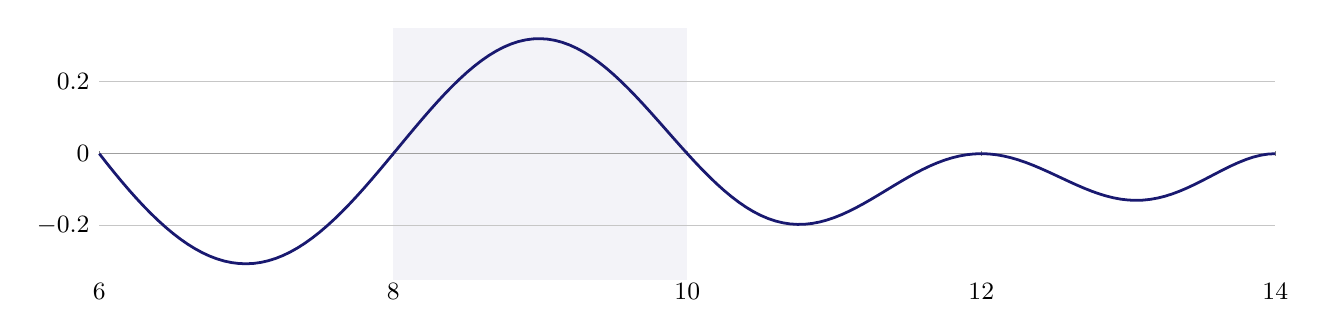
\begin{tikzpicture}[x=0.735in,y=1.8in,font=\small]
\fill[MidnightBlue!5] (8,-0.35) rectangle (10,0.35);
\draw[gray!45] (6,-0.2) -- (14,-0.2);
\draw[gray!45] (6,0.2) -- (14,0.2);
\draw[gray!75] (6,0) -- (14,0);
\foreach \x in {6,8,10,12,14}{\draw[gray] (\x,0.007)--(\x,-0.007);\node[below,fill=white,inner sep=1pt] at (\x,-0.35){\x};}
\node[left] at (6,-0.2) {$-0.2$};\node[left] at (6,0) {$0$};\node[left] at (6,0.2) {$0.2$};
\draw[MidnightBlue,line width=1pt] plot coordinates {
(6.00,0.00000000) (6.05,-0.02606861) (6.10,-0.05149120) (6.15,-0.07617761) (6.20,-0.10003824) (6.25,-0.12298444) (6.30,-0.14492906) (6.35,-0.16578685)
(6.40,-0.18547501) (6.45,-0.20391363) (6.50,-0.22102626) (6.55,-0.23674036) (6.60,-0.25098782) (6.65,-0.26370549) (6.70,-0.27483564) (6.75,-0.28432646)
(6.80,-0.29213255) (6.85,-0.29821535) (6.90,-0.30254356) (6.95,-0.30509360) (7.00,-0.30584992) (7.05,-0.30480539) (7.10,-0.30196160) (7.15,-0.29732909)
(7.20,-0.29092761) (7.25,-0.28278625) (7.30,-0.27294359) (7.35,-0.26144775) (7.40,-0.24835637) (7.45,-0.23373656) (7.50,-0.21766479) (7.55,-0.20022667)
(7.60,-0.18151672) (7.65,-0.16163799) (7.70,-0.14070174) (7.75,-0.11882687) (7.80,-0.09613945) (7.85,-0.07277211) (7.90,-0.04886330) (7.95,-0.02455663)
(8.00,0.00000000) (8.05,0.02465523) (8.10,0.04925517) (8.15,0.07364435) (8.20,0.09766677) (8.25,0.12116689) (8.30,0.14399078) (8.35,0.16598718)
(8.40,0.18700860) (8.45,0.20691250) (8.50,0.22556240) (8.55,0.24282893) (8.60,0.25859102) (8.65,0.27273688) (8.70,0.28516505) (8.75,0.29578535)
(8.80,0.30451979) (8.85,0.31130342) (8.90,0.31608501) (8.95,0.31882776) (9.00,0.31950985) (9.05,0.31812482) (9.10,0.31468194) (9.15,0.30920640)
(9.20,0.30173932) (9.25,0.29233773) (9.30,0.28107430) (9.35,0.26803700) (9.40,0.25332856) (9.45,0.23706580) (9.50,0.21937885) (9.55,0.20041018)
(9.60,0.18031346) (9.65,0.15925240) (9.70,0.13739934) (9.75,0.11493383) (9.80,0.09204101) (9.85,0.06890994) (9.90,0.04573189) (9.95,0.02269852)
(10.00,0.00000000) (10.05,-0.02217684) (10.10,-0.04365040) (10.15,-0.06424620) (10.20,-0.08379873) (10.25,-0.10215317) (10.30,-0.11916720) (10.35,-0.13471249)
(10.40,-0.14867630) (10.45,-0.16096275) (10.50,-0.17149402) (10.55,-0.18021138) (10.60,-0.18707597) (10.65,-0.19206937) (10.70,-0.19519404) (10.75,-0.19647334)
(10.80,-0.19595150) (10.85,-0.19369317) (10.90,-0.18978283) (10.95,-0.18432387) (11.00,-0.17743745) (11.05,-0.16926109) (11.10,-0.15994707) (11.15,-0.14966054)
(11.20,-0.13857748) (11.25,-0.12688244) (11.30,-0.11476616) (11.35,-0.10242302) (11.40,-0.09004839) (11.45,-0.07783597) (11.50,-0.06597503) (11.55,-0.05464770)
(11.60,-0.04402626) (11.65,-0.03427062) (11.70,-0.02552578) (11.75,-0.01791957) (11.80,-0.01156058) (11.85,-0.00653632) (11.90,-0.00291162) (11.95,-0.00072745)
(12.00,0.00000000) (12.05,-0.00072017) (12.10,-0.00285345) (12.15,-0.00634019) (12.20,-0.01109634) (12.25,-0.01701454) (12.30,-0.02396572) (12.35,-0.03180102)
(12.40,-0.04035419) (12.45,-0.04944429) (12.50,-0.05887877) (12.55,-0.06845681) (12.60,-0.07797295) (12.65,-0.08722093) (12.70,-0.09599756) (12.75,-0.10410683)
(12.80,-0.11136389) (12.85,-0.11759903) (12.90,-0.12266148) (12.95,-0.12642304) (13.00,-0.12878135) (13.05,-0.12966285) (13.10,-0.12902524) (13.15,-0.12685948)
(13.20,-0.12319118) (13.25,-0.11808139) (13.30,-0.11162664) (13.35,-0.10395841) (13.40,-0.09524171) (13.45,-0.08567302) (13.50,-0.07547741) (13.55,-0.06490502)
(13.60,-0.05422676) (13.65,-0.04372942) (13.70,-0.03371015) (13.75,-0.02447050) (13.80,-0.01630999) (13.85,-0.00951942) (13.90,-0.00437399) (13.95,-0.00112640)
(14.00,0.00000000)
};
\end{tikzpicture}
\caption{The signed physical profile of the Gon\c{c}alves--Vedana function in rank $48$. The abscissa is squared distance $s$. Multiplication by $10^9\exp(8(s-8)/3)/h_0$ makes successive extrema visible and preserves all signs and zeros. The shaded interval is the original forbidden annulus. The curve uses numerical quadrature; the endpoint estimates in the proof use rational series bounds.}
\end{figure}


\subsection{A shorter Gram test and an effective annulus for lattices}
\label{sec:compressed-window}
The rank-$43$ through $48$ entries in the lattice bounds of \cite[Table~1]{Zub} can be used in both factors of the projected-basis inequality in Corollary~\ref{cor:thick-48-blichfeldt}. With the tolerance $\epsilon$ of Theorem~\ref{thm:thick-window}, this reduces the squared cutoff for \emph{all} rank-$48$ lattices of squared minimum at least six to $228$.

Indeed set $U_0=U_1=1$ and start with $U_j=(2/\pi)^j\Gamma(2+j/2)^2$ for $j\ge2$. For each rank $j$ for which the quoted table is used, replace $U_j$ by its minimum with $(4/\pi)^j\Gamma(1+j/2)^2\Delta_j^2$, where $\Delta_j$ is the tabulated lattice density upper bound. Then $\gamma_j^j\le U_j$. Bound the next squared Gram--Schmidt length by $h_j$ obtained by rounding $(U_{48-j}U_j/6^j)^{1/(48-j)}$ upwards to a multiple of $10^{-4}$, with $0\le j<48$. It suffices to use $333/106<\pi<355/113$ in the favorable directions for all factors. The sum of these rational $h_j$ is less than $308$ and the sum of the two largest numbers $h_j+\tfrac14\sum_{i<j}h_i$ is less than $228$. The script \path{window_kz.py} verifies both comparisons by integer powers. The basis and signed-pair polarization proof of Corollary~\ref{cor:thick-48-blichfeldt} is then unchanged. The covering radius of a competing lattice of covolume at most one is at most $\sqrt{77}$, by successive rounding in this basis.

\begin{corollary}
If a lattice in dimension $48$ has squared minimum at least six and contains no vector of squared norm in $(8+10^{-130},10-10^{-130})$, then it has covolume at least one. Equality holds precisely for the extremal even unimodular lattices.
\end{corollary}
\begin{proof}
In the proof of Theorem~\ref{thm:numeric-annulus} take $R^2=228$. For a nonextremal lattice with covolume at most one there is a squared norm $10<u\le228$ with distance greater than $\epsilon/3>10^{-27}/3$ from the even integers. The same lower bound for $-h(u)$ holds. The estimate of Section~\ref{sec:profile} bounds the sum of all positive terms by $1304h_0e<10^{25}e$ when $e\le10^{-7}$. The sufficient decimal exponent becomes $58+24\log_{10}(R+1)+(\pi/\log 10)(2R+1)<130$; one may use $R<15.1$, $\log_{10}(16.1)<1.208$, $\pi<22/7$ and $\log 10>2.30$. Thus the positive terms cannot compensate the one strictly negative term, contradicting Poisson summation.
\end{proof}


\part{Poisson summation with lattice relations}

\section{Lattice tests on ordered pairs}
Fix a shortest allowed length $r$. Write $C=\{0\}\cup\{x\in\mathbb R^d:|x|\ge r\}$. A condition on $(x,y)$ suited to a lattice is that $ax+by\in C$ for every pair of integers $a,b$. Write $S$ for this set of pairs. Theorem 1.4 of Cohn, de Laat and Salmon (arXiv:2206.15373) uses just the four lengths of $x,y,x+y,x-y$. Their Remark 4.1 permits the full family. Working in the Schwartz class, the summation argument is short enough to give explicitly.

\begin{proposition}
Let $K$ be a real Schwartz function on $\mathbb R^d\times\mathbb R^d$. Suppose $K\le0$ on $S\setminus\{(0,0)\}$, $\widehat K\ge0$, and $\widehat K(0,0)>0$. Every lattice $L$ with minimum length at least $r$ satisfies
\begin{equation*}
 \frac1{\operatorname{covol}(L)}\le
 \left(\frac{K(0,0)}{\widehat K(0,0)}\right)^{1/2}.
\end{equation*}
Equality forces $K$ to vanish on all nonzero points of $L^2$, and $\widehat K$ to vanish on all nonzero points of $(L^*)^2$.
\end{proposition}
\begin{proof}
Poisson summation on $L\times L$ expresses the sum of $K$ on $L^2$ as $\operatorname{covol}(L)^{-2}$ times the sum of $\widehat K$ on $(L^*)^2$. The former is at most $K(0,0)$ and the latter, before multiplying by the covolume factor, is at least $\widehat K(0,0)$. All sums converge absolutely. Equality forces each term of each discarded sum to vanish.
\end{proof}

\subsection{The loss from joint radial symmetry}
Suppose $K(x,y)$ depends only on $(|x|^2+|y|^2)^{1/2}$. Each vector $(x,0)$ with $|x|\ge r$ belongs to $S$. Consequently $K$, regarded as a function on $\mathbb R^{2d}$, is a Cohn--Elkies test function with sign radius $r$. This gives a quantitative obstruction in dimension~48 without numerical optimization.

\begin{proposition}
Let $V=\pi^d r^{2d}/d!$. Every jointly radial $K$ as above satisfies
\begin{equation*}
 \left(\frac{K(0,0)}{\widehat K(0,0)}\right)^{1/2}\ge
 \left(\frac{2\zeta(2d)}{V}\right)^{1/2}.
\end{equation*}
For $d=48$ and $r^2=6$ the right side exceeds $1.23$. For $d=24n$ and $r^2=2n+2$ it exceeds $1$ for every $n\ge2$.
\end{proposition}
\begin{proof}
For a Haar-random lattice of covolume $D$ in $\mathbb R^{2d}$, Siegel's mean value theorem gives $V/(D\zeta(2d))$ for the expected number of primitive points in the open ball of radius $r$. Here the primitive variant follows from the usual formula by M\"obius inversion, since $2d>1$. Primitive points come in antipodal pairs. If $D>V/(2\zeta(2d))$, there is a lattice with no such points, and therefore with minimum length at least $r$. Apply the ordinary Poisson bound with $K$ on this lattice and pass to the limit in $D$. For $n=2$, $V=(6\pi)^{48}/48!$ lies between $1.3199$ and $1.3200$ (already $3.14159<\pi<3.14160$ suffices). For $n\ge3$ the elementary factorial lower bound $d!>(d/e)^d$ gives $V<(\pi e(1+1/n)/12)^{24n}\le(\pi e/9)^{24n}<1$.
\end{proof}

\subsection{Independent rotations of the two vectors}
A kernel invariant under independent rotations is allowed to distinguish the lengths $|x|$ and $|y|$. Nevertheless it discards exactly the angle on which the lattice constraints carry additional information. For every $u,v\in\{0\}\cup[r,\infty)$ one can choose orthogonal $x,y$ of lengths $u,v$ in $\mathbb R^d$, $d\ge2$. The equality $|ax+by|^2=a^2u^2+b^2v^2$ then shows $(x,y)\in S$. Independent rotational invariance therefore implies $K\le0$ on all of $(C\times C)\setminus\{(0,0)\}$. Conversely this condition suffices for the sign requirement on $S$.

A direct transfer of one-body dual certificates follows. Suppose $\mu$ and $\widehat\mu$ are nonnegative tempered measures on $\mathbb R^d$, $\mu$ is supported in $C$, $\mu(\{0\})=1$, and $\widehat\mu(\{0\})=b$. Then $\mu\otimes\mu$ has its only atom involving two zero vectors of mass one, and its Fourier transform is $\widehat\mu\otimes\widehat\mu$. Pairing a separately radial kernel with these measures yields $K(0,0)\ge b^2\widehat K(0,0)$. Evenness removes the reflection in Fourier inversion. Cohn, de Laat and Salmon prove the precise product formula in Proposition 4.7 of their paper: after taking the square root, the infimum for this full product sign domain is the ordinary one-body LP infimum. Independent rotational averaging preserves this product domain, so the formula applies to separately radial kernels. It does not settle the unrestricted angular problem.

\subsection{Exact angular conditions from the first shell}
Let $E$ be an extremal even unimodular lattice of rank $48$ and $X$ its shell of norm squared $6$. We use the spherical design identity for $X$ through degree six and $|X|=52\,416\,000$. For fixed $x\in X$ let $N_j$ count the $y\in X$ with $|\langle x,y\rangle|=j$. Integrality and the minimum restrict $j$ to $0,1,2,3,6$. Indeed, unless $y=\pm x$, both $x+y$ and $x-y$ have norm squared at least six. For the last value $N_6=2$. For $k=0,1,2,3$, spherical moments give
\begin{equation*}
 \sum_j N_j j^{2k}=|X|\,36^k\frac{(2k-1)!!}{\prod_{i=0}^{k-1}(48+2i)}.
\end{equation*}
The $k=0$ equation counts all points. The four remaining unknowns form a nonsingular Vandermonde system on $0,1,4,9$. The solution is
\begin{center}
\begin{tabular}{c|rrrrr}
$j$&0&1&2&3&6\\ \hline
$N_j$&23\,766\,960&25\,217\,568&3\,357\,774&73\,696&2
\end{tabular}
\end{center}

Assume $K$ is sharp for $E$. Joint rotations and the two independent changes of sign preserve $S$ and the Fourier inequalities. Average so that $K$ is invariant under these compact groups. At $|x|^2=|y|^2=6$ suppose $K(x,y)=p(\langle x,y\rangle^2)$ for a polynomial $p$. Then
\begin{equation*}
 z(z-1)^2(z-4)^2(z-9)(z-36)\mid p(z).
\end{equation*}
All five roots follow from the table and complementary slackness. For every $z\in[0,9]$ all the integral combinations of such vectors have admissible length. In fact, for $(a,b)\ne(0,0)$ their squared lengths are at least $6(a^2+b^2-|ab|)\ge6$. The roots at $1,4$ are therefore interior zeros of a polynomial of fixed weak sign. For the Fourier transform the corresponding necessary factor, if its shell restriction is a polynomial, is $z(z-1)^2(z-4)^2(z-9)^2(z-36)$. Its sign requirement holds on the whole interval $[0,36]$. These divisibilities allow either polynomial to vanish identically on this shell. They impose no degree requirement on kernels whose shell profiles already vanish identically.

No nonzero polynomial times a single nowhere vanishing Gaussian on $\mathbb R^{2d}$ can be an exact sharp kernel for a lattice. Complementary slackness would require that polynomial to vanish on the full-rank grid $E^2$ outside the origin. In linear coordinates carrying the grid to $\mathbb Z^{2d}$, fix all but one variable to integer values. The univariate polynomial vanishes at every integer, with at most one exception, hence vanishes identically. Repetition with the remaining variables proves the claim. Polynomial approximations can still be used for nonsharp upper bounds.

\subsection{A one-vector certificate using primitive lines}
Let $f$ be a real radial Schwartz function on $\mathbb R^d$, and set $A_f(t)=\sum_{k\ge1}f(kt)$ for $t>0$, using the radial profile. If $A_f(t)\le0$ for $t\ge r$, $A_{\widehat f}(s)\ge0$ for $s>0$, and $\widehat f(0)>0$, every lattice of minimum length at least $r$ satisfies $\operatorname{covol}(L)^{-1}\le f(0)/\widehat f(0)$. Indeed every nonzero lattice point is a positive integer multiple of a unique oriented primitive vector. Group the two absolutely convergent Poisson sums in this manner. This weakens the pointwise signs on both sides and gives a certificate specifically for lattices. It supplies no sharp $f$ on its own. Equality forces $A_f$ to vanish at all primitive lengths in $L$ and $A_{\widehat f}$ to vanish at all primitive lengths in $L^*$.

One can recover individual point values by M\"obius inversion on each ray. Explicitly, $f(t)=\sum_{k\ge1}\mu(k)A_f(kt)$ for $t>0$. Termwise differentiation is valid on compact subsets of $(0,\infty)$ by rapid decay. Both observations are important for attempts to use cancellations along a ray to remove an unwanted positive interval.

\begin{proposition}[A simple zero survives summation over multiples]
Suppose $t_0>r$, $f(kt_0)=0$ for every $k\ge1$, $f'(kt_0)=0$ for every $k\ge2$, and $f'(t_0)\ne0$. Then $A_f$ takes positive values arbitrarily close to $t_0$.
\end{proposition}
\begin{proof}
Local uniform convergence of the series and of its termwise derivative gives $A_f(t_0)=0$ and $A'_f(t_0)=\sum_{k\ge1} kf'(kt_0)=f'(t_0)$. Since $t_0$ is an interior point of $(r,\infty)$, a nonzero derivative forces values of both signs.
\end{proof}
In particular, a simple zero of a proposed constrained function at $\sqrt8$ cannot be repaired by primitive-line summation when its zeros at the integer multiples $k\sqrt8$, $k\ge2$, are double.

\subsection{Inheritance of the shell obstruction by primitive resummation}
For clarity, fix an extremal even unimodular lattice $E$ of rank~48 and write $R(n)=\#\{x\in E:|x|^2=2n\}$ and $b=131040/236364091$. Its theta series yields the coefficient bound $|R(n)-b\sigma_{23}(n)|\le4n^{12}$ for every $n\ge1$. One verification is to subtract the normalized $E_{24}$ from the theta series and expand the difference in the two normalized eigenforms in $S_{24}$. Their eigenvalues at $2$ are $540\pm12\sqrt{144169}$. The coefficients $c_\pm$ of these eigenforms satisfy $c_++c_-=-b$ and $c_+(540+12\sqrt{144169})+c_-(540-12\sqrt{144169})=-b(1+2^{23})$. Solving gives $|c_+|+|c_-|<2$. Deligne's bound $d(n)n^{23/2}$, together with $d(n)\le2\sqrt n$, proves the required estimate.

\begin{lemma}
For every $n\ge3$ the shell of squared norm $2n$ contains a primitive vector of $E$.
\end{lemma}
\begin{proof}
A nonprimitive shell point has the form $ky$, $k\ge2$, with $k^2\mid n$. The number of primitive points is therefore at least $R(n)-\sum_{k\ge2,\,k^2\mid n}R(n/k^2)$. Since $m^{23}\le\sigma_{23}(m)\le\zeta(23)m^{23}$, the resulting lower bound is
\begin{equation*}
 b n^{23}\bigl(1-\zeta(23)(\zeta(46)-1)\bigr)-4\zeta(24)n^{12}.
\end{equation*}
Integral comparison of the tails gives $\zeta(23),\zeta(24)<2$ and $\zeta(46)-1<1/4$. Now $b3^{11}>90$, so the expression is positive for $n\ge3$.
\end{proof}

Suppose the primitive-line certificate at $r=\sqrt6$ were exact for $E$. Its equality conditions and the lemma give $A_f(\sqrt{2m})=A_{\widehat f}(\sqrt{2m})=0$ for every $m\ge3$. The signs of these functions force $A_f'(\sqrt{2m})=0$ for $m>3$ and $A_{\widehat f}'(\sqrt{2m})=0$ for $m\ge3$. M\"obius inversion transfers the same value and derivative equalities to $f$ and $\widehat f$ themselves. Indeed a multiple $k\sqrt{2m}$ again has the form $\sqrt{2n}$ with $n=k^2m$. Absolute, locally uniform convergence after differentiation follows by applying the rapid decay estimates to $\sum_{k,\ell}k\ell |f'(k\ell t)|$. Scaling Poisson summation for $E$ now forces $f'(\sqrt6)=-48\widehat f(0)/(|X|\sqrt6)\ne0$. Thus any Fourier interpolation obstruction using just these shell values and slopes applies unchanged. In particular the invariant distribution of the modular construction in this manuscript excludes such a primitive-line certificate as well.

\subsection{The quantitative dual certificate survives primitive resummation}
A stronger conclusion follows directly from the positive shell measures of Section~\ref{sec:level-four}. Use the normalizations $r=\sqrt7$ and $D=2^{24}$ of that section. For either shell sequence $c_n=a_n$ or $c_n=b_n$, define its primitive coefficients for $n\ge1$ by
\begin{equation*}
 u_n=\sum_{k^2\mid n}\mu(k)c_{n/k^2}.
\end{equation*}
Then $c_n=\sum_{k^2\mid n}u_{n/k^2}$. We claim $u_n\ge0$ for every $n\ge1$ in both cases. The Eisenstein coefficient $E_n$ obeys $2^{-39}n^{23}<E_n<2^{-30}n^{23}$. For the upper bound, the displayed Eisenstein formula in Section~\ref{sec:level-four} and its version with $\alpha,\gamma$ exchanged give
\begin{equation*}
 E_n/n^{23}\le e\zeta(23)(4/D+2\cdot 4^{-23})<2^{-30}.
\end{equation*}
Writing $B=10\cdot2^{28}$, the cusp error is bounded by $Bn^{12}$. On removing square factors, the main term and accumulated errors therefore give
\begin{equation*}
 u_n\ge n^{23}\bigl(2^{-39}-2^{-30}(\zeta(46)-1)\bigr)
              -B\zeta(24)n^{12}.
\end{equation*}
Here we lower-bound a signed sum by subtracting the sum of absolute values of all its $k\ge2$ terms. Integral comparison gives $\zeta(46)-1<2^{-44}$ and $\zeta(24)<2$. The lower bound is positive for $n\ge128$, since $n^{11}\ge2^{77}$.

The small coefficients may be checked by integer recursion. Multiply $c_n$ by the fixed common denominator from the polynomial $P$, and compute $u_n=c_n-\sum_{k\ge2,\,k^2\mid n}u_{n/k^2}$ in increasing order. The script \texttt{packing48-primitive-dual.py} performs this computation for $1\le n\le127$. Its zero indices are $1,2,3,4,5,6,8$ on the physical side and $1,2,3,4,5$ on the Fourier side. All other coefficients in this range are positive.

Writing $u_n^a,u_n^b$ for the two primitive sequences, the shell identity for every radial Schwartz $f$ is now
\begin{equation*}
 a_0 f(0)+\sum_{n\ge1}u_n^a A_f(\sqrt n)
 = b_0\widehat f(0)+\sum_{n\ge1}u_n^b A_{\widehat f}(\sqrt n).
\end{equation*}
Rapid decay and the polynomial coefficient bound justify reordering. Under the primitive sign conditions the first sum is nonpositive, because its first possible shell is $n=7$, and the second sum is nonnegative. Scaling as in Theorem~\ref{thm:level-four-dual} gives the same factor exceeding $8.6268$ for every primitive-line certificate. This also applies if only one side is permitted cancellation along multiples.


\section{\texorpdfstring{The level-$49$ obstruction on primitive rays and a separating angular inequality}{The level-49 obstruction on primitive rays and a separating angular inequality}}
\label{sec:primitive49}
For a Schwartz function $f$ write $A_f(x)=\sum_{k\geq1}f(kx)$ for
$x\ne0$. The cone defined by $A_f(x)\leq0$ for $|x|\geq r$ and
$A_{\widehat f}(y)\geq0$ for $y\ne0$ admits more tests than the ordinary
two-point cone. It gives lattice upper bounds by grouping the two
Poisson sums along oriented primitive vectors. The additional freedom
still does not reach the lattice-specific upper bound of Zubrilina.

\begin{theorem}\label{thm:primitive49}
Every Schwartz test in the primitive-ray cone in dimension $48$, with
$\widehat f(0)>0$, gives a density bound at least
$(454/25)\delta_{\rm ext}$.
\end{theorem}
\begin{proof}
Rotational averaging permits a radial test. Define, for $n>0$,
$u_n=\sum_{k^2\mid n}\mu(k)c_{n/k^2}$ for either sequence
$c_n=a_n,b_n$ of Section~\ref{sec:level49}. We prove that both
sequences $u_n$ are nonnegative. With the notation of that section, let
$Q=7^{23}$ and write $n=7^j m$ with $7\nmid m$.
Square-divisor inversion sends $\sigma_{23}(m)$ to
$m^{23}\prod_{\ell\mid m}(1+\ell^{-23})$, with $\ell$ running over
primes. This follows by multiplicativity from
$\sigma_{23}(\ell^h)-\sigma_{23}(\ell^{h-2})
=\ell^{23h}+\ell^{23(h-1)}$ for $h\geq1$, taking terms at negative
exponents as zero. Removing a square relatively prime to $7$
preserves $\chi(m)$. Define $S_j=1+Q+\cdots+Q^j$ for $j\geq0$,
with $S_j=0$ for $j<0$, and set
$v_j=A S_j+B S_{j-1}+C S_{j-2}+T\chi(m)\mathbf 1_{j=0}$.
The $7$-adic multiplier is now
$Q^{-j}(v_j-\mathbf 1_{j\geq2}v_{j-2})$.
Thus $u_n$'s Eisenstein part is bounded below by $m_0n^{23}$, where
$m_0/e_{24}$ is the minimum of
\[
 A-|T|,\quad
 \frac{A(1+Q)+B}{Q},\quad
 \frac{A(Q+Q^2)+B(1+Q)+C-|T|}{Q^2},\quad
 (1+Q^{-1})(A+B/Q+C/Q^2).
\]
The fourth expression applies at every $j\geq3$.
Rational substitution gives lower bounds $5.0842\cdot10^{-25}$ and
$1.2726\cdot10^{-24}$ on the respective $m_0$. The transformed cusp
coefficients have absolute value at most
$73\zeta(24)n^{12}<74n^{12}$, since
$\zeta(24)-1\le2^{-24}+2^{-23}/23$. The physical primitive
coefficients are therefore positive for $n\ge240$, and the transformed
ones for $n\ge220$.

In the remaining range the supplied verifier recomputes the integer
coefficients by both square-divisor inversion and subtraction of the
contributions of smaller primitive shells. It finds zeros exactly at
indices $1,\ldots,23$ physically and $1,\ldots,18$ on the Fourier
side. All other checked coefficients are positive. Absolute
convergence and the identity $c_n=\sum_{k^2\mid n}u_{n/k^2}$ now give
\[
 f(0)+\sum_{n\ge1}u_n^a A_f(\sqrt{2n/7})
   =b_0\widehat f(0)+\sum_{n\ge1}u_n^b
       A_{\widehat f}(\sqrt{2n/7}).
\]
The stipulated signs give the same inequality and density factor as
in Theorem~\ref{thm:49}.
\end{proof}

\subsection{An angular restriction violated by the shell measure}
Write $r$ for the lattice minimum, $s=501/500$, and $t=1-1/(2s^2)$.
The vectors in the shell $r\le|x|\le sr$, divided individually by
their norms, form an antipodal spherical code. Distinct non-antipodal
directions have absolute inner product at most $t$. Indeed
$|x\pm y|\ge r$, and $(a^2+b^2-r^2)/(2ab)$ increases in both
variables for $r\le a,b\le sr$, because $s^2<2$.
There are no proportional vectors with distinct positive lengths in
this shell, as $s<2$ and each nonprimitive lattice vector has length at
least $2r$.

Put $p(z)=-7+1770z-51272z^2+308096z^3$ and
$H(x)=(x^2-t^2)p(x^2)^2$.
In dimension $48$ its coefficients in the normalized even Gegenbauer
basis of degrees $0$ through $14$ are all strictly positive.
This finite arithmetic check uses $C_0=1$, $C_1=x$ and
$(j+45)C_j=(2j+44)xC_{j-1}-(j-1)C_{j-2}$. The addition theorem
therefore gives a lower bound $M^2H_0$ for the sum over ordered
pairs of a spherical code of size $M$. Each off-diagonal,
non-antipodal term is nonpositive. Consequently
\[
 M\leq B:=\frac{2H(1)}{H_0}
      =\frac{2158380250092360000000}{2585621548829}
      <834762633.
\]
At $s=1$ the same polynomial, with $t=1/2$, gives the bound
$8378218800/11$ on the size of a minimal shell.
The exact rational verifier checks both Gegenbauer expansions. For the
certificate of Section~\ref{sec:level49}, $a_{24}>941000000$.
Since $24s^2<25$, the whole first-shell mass already violates the
short-shell upper bound $B$. This proves directly that the formal
radial measures fail an angular constraint obeyed by every lattice.

\subsection{Effect of a single short-shell constraint on the test bound}
Take radial Schwartz functions and allow a variable $h\ge0$ with
$A_f(x)\le h$ on $r\le|x|\le sr$ and $A_f(x)\le0$ for $|x|>sr$.
Keep $A_{\widehat f}(y)\ge0$ for $y\ne0$ and $\widehat f(0)>0$.
The resulting lattice density upper bound is
$v_{48}(r/2)^{48}(f(0)+Bh)/\widehat f(0)$, as the entire short
shell consists of primitive points. Replacing $A_f,A_{\widehat f}$
by $f,\widehat f$ gives the corresponding ordinary scalar program
with the same angular penalty.

A convex combination of two summation formulas gives a lower bound
on the infimum of either enlarged program. Set $r=\sqrt{48/7}$
and let $\theta=B/a_{24}$. Use the unmodified level-$49$ measure with
weight $\theta$. Use its spatial dilation by $\tau>s$ with weight
$1-\theta$. The transform of a spatially dilated measure has its
origin mass multiplied by $\tau^{-48}$ and its nonzero shells dilated
by $1/\tau$. Both measures still have nonnegative primitive coefficients
after dilation. Their mixture gives exactly $B$ points of mass on the
short spatial shell and has zero mass between $r$ and its boundary
apart from the first shell. Applying the two signs and taking
$\tau\downarrow s$ shows that every resulting upper bound is at least
\[
 \frac{907}{50}
 \bigl(\theta+(1-\theta)(500/501)^{48}\bigr)\,
 \delta_{\rm ext}
 >17.9518\,\delta_{\rm ext}.
\]
This estimate allows a single short-shell occupancy constraint; it does
not impose the full Gram-matrix geometry of a lattice. For upper
constraints of arbitrary shape supported only in $[r,sr]$, the dilated
measure alone evades every such nonnegative occupancy bound. It still
gives the factor $(454/25)s^{-48}>16.48$ at the displayed value of $s$.


\section{One-vector bounds with arbitrary congruence conditions}
\label{sec:color}
Can a Fourier proof use the coordinates of a lattice vector modulo an integer to distinguish a lattice from the positive modular distribution of Theorem~\ref{thm:49}? We give a general lifting theorem. Its hypotheses ask for positive primitive masses on both sides. Its conclusion covers tests that distinguish every individual residue in a fixed basis, with any modulus, and allows joint cancellation along each primitive ray. The modulus may be chosen separately for each attempted bound.

Fix $d\ge2$, $q\ge1$, and put $A=(\mathbb Z/q\mathbb Z)^d$. Write $D_s\rho$ for pushforward of a measure under $x\mapsto sx$, so that $\widehat{D_s\rho}=s^{-d}D_{1/s}\widehat\rho$. Let $\rho$ and $\sigma=\widehat\rho$ be even, radial tempered measures with positive origin masses $a,b$, respectively. Suppose they admit decompositions
\begin{equation*}
 \rho=a\delta_0+\sum_{k\ge1}D_k P,\qquad
 \sigma=b\delta_0+\sum_{k\ge1}D_k Q
\end{equation*}
with $P,Q$ positive measures supported outside neighborhoods of zero. Assume that all positive mass of $P$ has radius at least $r$. The sums are locally finite, and pairing with Schwartz functions is absolutely convergent by positivity and temperedness. No integrality of a radius is assumed in this construction.

Let $h(c)=\gcd(q,c_1,\ldots,c_d)$, with $h(0)=q$. The primitive residues $u\in A$ are those with $h(u)=1$ (for $q=1$ this includes the unique residue). For a general divisor $h\mid q$ write $A_h=\{c:h(c)=h\}$. It has $J_d(q/h)$ elements, where $J_d(n)=n^d\prod_{p\mid n}(1-p^{-d})$. Distribute the measure $P$ uniformly over the primitive residues and give its $k$th multiples the labels $ku$. More explicitly, let
\begin{equation*}
 \rho_c=\mathbf1_{c=0}a\delta_0+
 \frac1{J_d(q)}\sum_{u\in A_1}\sum_{k\ge1:\ ku=c}D_kP.
\end{equation*}
Use $Q,b$ to define $\sigma_t$ in the same way. They are positive, and their sums over labels equal the original measures.

\begin{lemma}[Finite Fourier compatibility]\label{lem:color}
As tempered distributions, for every $c\in A$,
\begin{equation*}
 \widehat\rho_c=q^{-d}\sum_{t\in A}
    e^{-2\pi i c\cdot t/q}\,D_{1/q}\sigma_t.
\end{equation*}
\end{lemma}
\begin{proof}
Multiplication by $k$ maps a uniformly random primitive residue to a uniformly random element of $A_{\gcd(k,q)}$. Indeed the assertion splits over prime powers. For $q=p^s$ and $v_p(k)=j<s$, reduction of primitive residue vectors to modulus $p^{s-j}$ has fibers of equal cardinality, the unit part of $k$ is invertible, and multiplication by $p^j$ puts the image in the desired orbit. When $j\ge s$ the image is zero. In particular all measures $\rho_c$ in an orbit coincide, as do the $\sigma_t$. With $\mu_{\rm M}$ denoting the arithmetic M\"obius function, inclusion--exclusion gives
\begin{equation*}
 \sum_{c\in A_h}\rho_c=\sum_{j\mid q/h}\mu_{\rm M}(j)D_{hj}\rho,\qquad
 \sum_{t:l\mid t} \sigma_t=D_l\sigma\quad(l\mid q),
\end{equation*}
where $l\mid t$ means divisibility of every coordinate. These identities hold also at zero, where the first sum has mass $a$ only when $h=q$. On the character side inclusion--exclusion gives
\begin{equation*}
 \sum_{c\in A_h}e^{-2\pi i c\cdot t/q}
   =\sum_{j\mid q/h}\mu_{\rm M}(j)
      \big(q/(hj)\big)^d\mathbf1_{q/(hj)\mid t}.
\end{equation*}
Summing the claimed identity over $c\in A_h$ now gives on each side
$\sum_{j\mid q/h}\mu_{\rm M}(j)(hj)^{-d}D_{1/(hj)}\sigma$.
The right side in the lemma is constant on $A_h$, by the transitive action of $\mathrm{GL}_d(\mathbb Z/q\mathbb Z)$ and the contragredient substitution in $t$. Transitivity follows over each prime power by extending a primitive vector to a basis, then combining by the Chinese remainder theorem. Division by $J_d(q/h)$ proves the assertion.
\end{proof}

Writing $S_q$ for the splitting into residues and $\mathcal F_A$ for the unnormalized finite Fourier transform in the label, the lemma is the commutativity of
\begin{equation*}
\begin{tikzcd}[column sep=large,row sep=large]
 \rho \arrow[r,"\mathcal F"] \arrow[d,"S_q"'] &
 \sigma \arrow[d,"q^{-d}D_{1/q}\mathcal F_A S_q"] \\
 (\rho_c)_{c\in A} \arrow[r,"\mathcal F_{\mathbb R^d}"'] &
 (\widehat\rho_c)_{c\in A}
\end{tikzcd}
\end{equation*}
The formula agrees exactly with Poisson summation in residue classes. In a based lattice $L=B\mathbb Z^d$ of covolume $V$, the Fourier transform of the comb on $Bc+qL$ is $(q^d V)^{-1}$ times the comb on $q^{-1}L^*$ with phase $e^{-2\pi i c\cdot t/q}$ at $B^{-\mathsf T}t/q$, now with $t\in\mathbb Z^d$. Let $f_c$ be real even Schwartz functions, and put
$G_t(\xi)=\sum_c \cos(2\pi c\cdot t/q)\widehat f_c(\xi)$.
Taking the real part after summing over labels gives the same identity for the even functions. One can make any real physical test even by simultaneously averaging over the sign of the argument for each label if both signs are feasible uniformly; the theorem below only needs the stated even class.

\begin{theorem}[Congruence and primitive-ray tests]\label{thm:coloredLP}
Suppose $G_0(0)>0$. Assume that for each $u\in A_1$ the inequalities
\begin{equation*}
 \sum_{k\ge1}f_{ku}(kx)\le0\quad(|x|\ge r),\qquad
 \sum_{k\ge1}G_{ku}(ky)\ge0\quad (y\ne0)
\end{equation*}
hold. The resulting upper bound on $1/V$ for a lattice of minimum length at least $r$ is $q^d f_0(0)/G_0(0)$. Under the hypotheses on the positive pair $\rho,\sigma$ one necessarily has
$q^d f_0(0)/G_0(0)\ge b/a$. For $d=48$, after scaling to $r=\sqrt6$, the level-$49$ certificate imposes the factor $454/25$ on every bound in this family.
\end{theorem}
\begin{proof}
For actual lattices sum over primitive coordinate vectors and their positive integer multiples. Primitive integer vectors reduce to primitive residues modulo $q$. Thus the nonzero physical contribution has sum at most zero and the nonzero dual contribution has sum at least zero. The two zero terms of Poisson summation are $f_0(0)$ and $G_0(0)/(q^d V)$.

For the modular obstruction use Lemma~\ref{lem:color}. Pair with the respective tests and sum over $c$. On the physical side the primitive-label construction gives a contribution at most $af_0(0)$. On the dual side the integral of the nonzero contributions is nonnegative, by the same construction at argument $y/q$; its zero term is $bG_0(0)/q^d$. For even functions the Fourier involution introduces no reflection. All reordered sums converge by the stated absolute convergence. This proves the inequality. For the last assertion apply the level-$49$ primitive coefficient bounds in this manuscript and scale all radii as in Theorem~\ref{thm:49}.
\end{proof}

Each pointwise physical or dual sign restriction implies the corresponding ray-sum restriction. Several finite moduli used simultaneously can be replaced by their least common multiple by pulling the physical tests back to it; the Fourier character sums vanish on the additional frequencies by orthogonality. This theorem concerns one lattice vector and the arithmetic of its multiples. The residue label of a second vector, with joint rank or determinant restrictions, supplies information outside its hypotheses.


\section{An angular obstruction and a nonseparable Fourier kernel}
\label{sec:angular48}
Let $r$ denote the chosen minimum length and $S$ the set of pairs $(x,y)$ whose integral combinations are zero or have length at least $r$. This section gives two results for the pair-kernel program. One locates the first angular degree at which the two-point dual certificate can distinguish lattice angles from independent uniform angles. The other constructs a feasible perturbation in precisely that degree. Throughout the dimension of each vector is $48$.

\subsection{Positive quadrature on admissible angles}
Take $x,y$ independently uniform on spheres of positive radii $u,v$. The cosine $t=\langle x,y\rangle/(uv)$ has probability measure $\nu$ proportional to $(1-t^2)^{45/2}\,dt$ on $[-1,1]$. Its odd moments vanish and $z=t^2$ has moments $m_0=1$, $m_{j+1}/m_j=(2j+1)/(48+2j)$.

\begin{theorem}
In the pair-kernel bound, suppose that after averaging simultaneous rotations, the dependence of $K(x,y)$ on $t$ at every fixed pair of nonzero radii is polynomial of degree at most $15$. Then the density upper bound furnished by $K$ is at least $8.6268$ times the density of an extremal lattice in rank~48.
\end{theorem}

\begin{proof}
Use the certificate of Section~\ref{sec:level-four}, with physical scale $r=\sqrt7$. Let $\mu$ be its radial physical measure and $\widehat\mu$ the positive transformed measure. The nonzero shells of $\mu$ have radius $\sqrt7$ or at least $3$, since the coefficient at $n=8$ vanishes. We show that the independent angular average of $K$ is nonpositive on every pair of radii of $\mu$, except the double origin. When one radius vanishes this follows immediately from the lattice sign condition.

The eight-node Gaussian quadrature for $\nu$ has positive weights, integrates polynomials of degree at most $15$, and has all its nodes in $(-11/20,11/20)$. For an exact check, its monic Gegenbauer polynomials satisfy $p_0=1$, $p_1=t$, and $p_{j+1}=tp_j-j(j+45)p_{j-1}/(4(j+23)(j+22))$. At $t=1/2$ the values for $j=1,\ldots,7$ are $1/2,11/48,19/200,181/5200,121/11232,263/104832,1/4176$, all positive. These are the leading principal minors of $tI-J_7$ for the Jacobi matrix, so all roots through degree seven lie below $1/2$. At $11/20$ they remain positive, and $p_8(11/20)=6729608063/20044800000000>0$. The same test for $J_8$ and symmetry give the asserted bound.

If $u,v$ are nonzero support radii and at least one is $\ge3$, all eight quadrature angles belong to $S$. For $a,b\in\mathbb Z\setminus\{0\}$,
\begin{equation*}
 |ax+by|^2\ge 2|ab|uv(1-|t|)\ge 2\sqrt7\cdot3(1-11/20)>7.
\end{equation*}
The cases $ab=0$ use $u,v\ge\sqrt7$. Thus the angular average is nonpositive for all these pairs.

It remains to integrate on the shell $u=v=\sqrt7$. Apply positive five-node Gauss--Lobatto quadrature on $[0,1]$ for the distribution of $z=t^2$. Its endpoints are $0,1$ and its three interior nodes are the roots of the degree-three polynomial orthogonal for $z(1-z)d\nu_z$, where $\nu_z$ is the distribution of $z$. The quadrature integrates through degree seven. Division by the degree-five product $z(1-z)p_3(z)$ shows exactness through degree seven by orthogonality and interpolation. For an interior node $\xi$, the nonnegative polynomial $z(1-z)(p_3(z)/(z-\xi))^2$ is zero at all other nodes and positive at $\xi$, proving positivity of that weight. For the endpoint $0$ use $(1-z)p_3(z)^2$, and for $1$ use $z p_3(z)^2$.

Each interior node is less than $1/4$. The monic orthogonal polynomials of degrees $1,2,3$ for the modified measure are, by the moment formula above,
\begin{align*}
 z-3/52,\qquad z^2-5z/28+5/1008,\qquad
 z^3-7z^2/20+7z/232-1/1856 .
\end{align*}
Their values at $1/4$ are $5/26,23/1008,7/9280$, respectively. The positive-definite Jacobi-matrix test applies once more. For each of the resulting $z$ take both signs of $t=\sqrt z$ with equal weights. If $|t|\le1/2$, then $|ax+by|^2\ge 7(a^2+b^2-|ab|)\ge7$ for nonzero $(a,b)$. At $z=1$, the equal-length vectors coincide up to sign, and their integer combinations also satisfy the required condition. Symmetry handles the odd moments through degree $15$. This proves the desired sign for the independent angular average on the remaining shell pair.

Finally pair $K$ with $\mu\otimes\mu$. On the physical side the double origin contributes $K(0,0)$ and the angular averages of all remaining terms are nonpositive. On the frequency side all terms are nonnegative, giving $K(0,0)\ge b_0^2\widehat K(0,0)$ with $b_0=3789481/17760256$. The factor in the density bound follows by taking square roots and comparing the two radii as in Section~\ref{sec:level-four}.
\end{proof}

\subsection{The degree-sixteen separation}
For two vectors both of length $r$, the exact admissible angles satisfy $z\in[0,1/4]\cup\{1\}$. Indeed the shortest of $x+y,x-y$ excludes every other value. The integer-combination inequality in the preceding proof gives the converse. Define
\begin{equation*}
 h(z)=z^3-\frac{221}{1328}z^2+\frac{885}{154048}z-\frac7{308096},
 \qquad P(z)=(z-1/4)(1-z)h(z)^2.
\end{equation*}
It is nonpositive on this entire admissible set. Yet its mean under independent uniform angles is $6817867/9955264993689600>0$, by the moments $m_j$. Thus no positive quadrature on the first-shell admissible angles can agree with independent uniform angles through degree $16$ in $t$. Combined with the previous theorem, this identifies an exact angular threshold for the indicated quadrature reduction. The construction of $h$ is reproducible: its leading coefficient is one and the three lower coefficients solve $\int z^j(1/4-z)(1-z)h(z)\,d\nu_z=0$ for $0\le j\le2$.

\subsection{A nonseparable trial function with both Fourier signs}
Normalize $r=1$ and put $U=|x|^2$, $V=|y|^2$, $W=\langle x,y\rangle$. Where $UV>0$ let $z=W^2/(UV)$ and $A^2=(U+V-1)^2/(4UV)$. The function
\begin{equation*}
 G(x,y)=(UV)^{11}(z-A^2)(1-z)h(z)^2 e^{-34(U+V)}
\end{equation*}
extends by a polynomial times a Gaussian across $UV=0$. In fact its polynomial part is $(UV)^3[4W^2-(U+V-1)^2](UV-W^2)[(UV)^3h(W^2/(UV))]^2/4$. If $(x,y)\in S$ with $x\ne\pm y$ and $UV>0$, the inequalities $|x\pm y|\ge1$ give $2|W|\le U+V-1$. If $x=\pm y$, the Gram determinant vanishes. The same formula vanishes on either coordinate axis. Hence $G\le0$ on $S$ and $G(0,0)=0$.

\begin{proposition}
For all sufficiently small $\varepsilon>0$, the Schwartz function
\begin{equation*}
 K_\varepsilon(x,y)=(1-U-V)e^{-49(U+V)}+\varepsilon G(x,y)
\end{equation*}
is feasible for the lattice pair-kernel bound at $r=1$. Its ratio $K_\varepsilon(0,0)/\widehat K_\varepsilon(0,0)$ is strictly smaller than that of the first term alone, which has the optimum Gaussian scale within the family $(1-U-V)e^{-a(U+V)}$.
\end{proposition}
\begin{proof}
On $S\setminus\{(0,0)\}$ at least one nonzero vector has squared length at least one. This verifies the physical sign. On $\mathbb R^{96}$ the Fourier transform of $(1-|w|^2)e^{-a|w|^2}$ is
\begin{equation*}
 (\pi/a)^{48}\left(1-48/a+\pi^2|\xi|^2/a^2\right)e^{-\pi^2|\xi|^2/a}.
\end{equation*}
It is strictly positive for $a>48$. Maximizing its value at zero in $a$ gives $a=49$. The transform of $G$ is a polynomial times $e^{-\pi^2|\xi|^2/34}$, so $\widehat G/\widehat K_0$ is bounded. For instance take any $0<\varepsilon<(1+\|\widehat G/\widehat K_0\|_\infty)^{-1}$.

It remains to prove $\widehat G(0,0)>0$. In its integral, absorb $(UV)^{11}e^{-34(U+V)}$ into the two radial weights. Up to a positive factor the expectations of the radial variables are now taken under independent gamma laws of shape $35$ and rate $34$. They are independent of $z$. In particular $\mathbb E[U]=35/34$ and $\mathbb E[1/U]=1$. Expanding $(U+V-1)^2/(4UV)$ gives $\mathbb E[A^2]=1/4+1/68$. The spherical moments give
\begin{equation*}
 \frac{\mathbb E[z(1-z)h(z)^2]}{\mathbb E[(1-z)h(z)^2]}
 =\frac{67213}{253580}>\frac14+\frac1{68}.
\end{equation*}
Thus $\widehat G(0,0)>0$. The numerator of the test-function ratio is independent of $\varepsilon$ and its denominator strictly increases.
\end{proof}

The perturbation certifies an angular improvement for this particular Gaussian family. Neither its existence nor the first-shell angular threshold gives a density bound matching the extremal lattice.

One completely explicit choice is $\varepsilon=2^{-400}$. Here are bounds that avoid a numerical minimization in the Fourier variables. Write $G=P e^{-34|w|^2}$ on $\mathbb R^{96}$. For complex $w$ of Hermitian length $T$ one has $|U|+|V|\le T^2$ and $|W|\le T^2$, interpreting $U,V,W$ by their bilinear polynomial extensions. The polynomial $h$ has coefficient absolute sum below two. The displayed polynomial formula for $P$ then gives $|P(w)|\le10(1+T)^{44}$. Completing the square, or differentiating the Gaussian transform, yields
\begin{equation*}
 \widehat G(\xi)=(\pi/34)^{48}e^{-\pi^2|\xi|^2/34}
 \mathbb E\big[P(\eta-i\pi\xi/34)\big],
\end{equation*}
where $\eta$ has real Gaussian density proportional to $e^{-34|\eta|^2}$. Its moment $\mathbb E|\eta|^{44}=(48\cdots69)/34^{22}<3^{22}$. Thus $\mathbb E(1+|\eta|)^{44}<2^{81}$. For $t=|\xi|$, the polynomial expectation is bounded by $10\cdot2^{81}(1+t)^{44}$. Moreover $\pi^2(1/34-1/49)>1/16$, and
\begin{equation*}
 (1+t)^{44}e^{-t^2/16}\le2^{44}(1+(352/e)^{22})<2^{243}.
\end{equation*}
Using the lower bound $\widehat K_0(\xi)\ge(\pi/49)^{48}e^{-\pi^2t^2/49}/49$ and $49(49/34)^{48}<2^{54}$ gives $\|\widehat G/\widehat K_0\|_\infty<2^{382}$. This proves feasibility for the stated coefficient. The improvement in the zero-frequency denominator can also be written exactly. Its relative coefficient $\widehat G(0)/\widehat K_0(0)$ equals
\begin{equation*}
 \frac{49^{49}(34!)^2}{34^{70}(23!)^2}
 \frac{121239461}{2665441917665280}\frac{1511}{4310860}.
\end{equation*}
This is approximately $0.0008590$ before multiplication by $\varepsilon$. The baseline density bound is $7(49/(6\pi))^{24}$ times the target, approximately $6.35\cdot10^{10}$. The explicit example is therefore quantitatively weak despite its strict improvement.

\subsection{A dimension-dependent limit on angular truncation}
Some of the preceding angular loss is independent of the particular dual certificate and of the extremal lattice. In dimension $d\ge4$, let $J_m$ be the $m$-node Jacobi matrix for the cosine of independent uniform directions. If its nodes lie in $[-1/2,1/2]$, every feasible pair kernel of cosine degree at most $2m-1$ can be replaced, without changing its ratio, by one invariant under independent rotations and nonpositive on the full product sign set. Indeed for any two nonzero radii $u,v\ge r$ and such a node $t$, every integral combination with both coefficients nonzero has squared length at least $2uv(1-|t|)\ge r^2$. Integrate the kernel by positive Gaussian quadrature at these nodes and handle the axes directly. The resulting independent angular average preserves positivity of the Fourier transform and both origin values. Thus Proposition~4.7 of Cohn, de Laat and Salmon identifies the infimum at this angular truncation with the ordinary scalar LP infimum under its hypotheses. In rank $48$ the seven-node calculation gives cosine degree $13$ irrespective of the scalar bound's actual value.

The squared off-diagonal entries of $J_m$ are $\beta_j=j(j+d-3)/((2j+d-2)(2j+d-4))$ for $1\le j<m$. They increase with $j$ for $d>4$ and are constant for $d=4$, as follows by writing them as $\tfrac14[1-(d-2)(d-4)/((2j+d-2)(2j+d-4))]$. The absolute values of all nodes are at most $2\sqrt{\beta_{m-1}}$ by the row-sum bound. If $m/d\to c$ with $0<c<(2/\sqrt3-1)/2$, this upper bound tends to $2\sqrt{c(c+1)}/(2c+1)<1/2$. Hence in large dimensions angular degrees up to $(2/\sqrt3-1-o(1))d$ can be insufficient to improve on the scalar LP; more precisely, every fixed smaller coefficient gives this conclusion for all sufficiently large $d$.

This coefficient is asymptotically sharp for the proposed quadrature supported in $[-1/2,1/2]$. Any positive measure on $[-a,a]$ reproducing the cosine moments through degree $2m-1$ has $\|J_m\|\le a$: on polynomials of degree below $m$, the inner product and the quadratic form for multiplication by $t$ depend only on those moments. Conversely Gaussian quadrature realizes the bound with $a=\|J_m\|$. In the regime $m/d\to c>0$, take the last $s=\lfloor\sqrt d\rfloor$ indices of $J_m$. Its nonnegative off-diagonal entries are at least $\sqrt{\beta_{m-s}}$, so the positive sine eigenvector of the constant-coefficient path matrix gives
\begin{equation*}
 2\sqrt{\beta_{m-s}}\cos(\pi/(s+1))
 \le\|J_m\|\le 2\sqrt{\beta_{m-1}}.
\end{equation*}
Both ends have limit $2\sqrt{c(c+1)}/(2c+1)$. At larger angular degrees the one fixed positive quadrature fails; different measures depending on the radii or a different proof may still impose an obstruction.


\section{The period cylinder over an offending vector}
Fix $t\in(\sqrt8,\sqrt{10})$ and normalize the minimum to $r=\sqrt6$. A lattice $L$ with a vector of length $t$ admits the following lower-dimensional description. The vector $v$ is primitive since $t<2r$. Project orthogonally along $v$ onto a copy of $\mathbb R^{47}$. A basis extending $v$ shows the image $Q$ is a full lattice and the kernel in $L$ is $\mathbb Zv$. The vertical coordinate modulo $t$ therefore defines a homomorphism $h:Q\to\mathbb R/t\mathbb Z$. Conversely $Q,h$ recover $L$ as the full preimage of the graph of $h$ under reduction modulo $t$ in the vertical coordinate. Its covolume is $t\operatorname{covol}(Q)$. With $\|\theta\|_t=\min_{k\in\mathbb Z}|\theta-kt|$, its minimum is at least $r$ exactly when
\begin{equation*}
 |x|^2+\|h(x)\|_t^2\ge6\qquad (0\ne x\in Q).
\end{equation*}
Here $t>r$ controls the pure vertical vectors. In particular $\min(Q)^2\ge 6-t^2/4$. Any clique of projected points with squared distances at most $s<6$ maps to circle points separated by at least $\sqrt{6-s}$, so a clique of at least two points has size at most $\lfloor t/\sqrt{6-s}\rfloor$ by summing cyclic gaps. In particular the graph with squared edge lengths strictly below $6-t^2/9$ is triangle-free.

\subsection{Tests with finitely many circle harmonics}
Use Haar measure $dx\,d\theta$ on $\mathbb R^{47}\times\mathbb R/t\mathbb Z$, so the circle has mass $t$. For a real Schwartz function in the Euclidean argument with a trigonometric polynomial in the circle argument, require $F(x,\theta)\le0$ whenever $|x|^2+\|\theta\|_t^2\ge6$ and require every coefficient of its Euclidean--circle Fourier transform to be nonnegative. Suppose also that the zero frequency $\widehat F(0,0)>0$. Poisson summation for the graph of $h$ bounds the inverse covolume of $L$ by $F(0,0)/\widehat F(0,0)$. To see it directly, expand in the circle frequencies. For the $k$th harmonic one obtains Poisson summation on $Q$ twisted by the character $x\mapsto e^{2\pi i k h(x)/t}$, hence a nonnegative sum on a translate of $Q^*$. The constant term at zero has the factor $1/(t\operatorname{covol}(Q))$ in the stated normalization.

\begin{proposition}
At every $t\in[\sqrt8,\sqrt{10}]$, a valid cylinder test using only frequencies $|k|\le3$ gives an inverse covolume bound strictly greater than $1.078$. For $|k|\le2$ the bound exceeds $1.59$ and for $|k|\le1$ it exceeds $5.08$.
\end{proposition}
\begin{proof}
Put $m=1,2$, or $3$. Denote the constant circle coefficient by $a(x)=t^{-1}\int F(x,\theta)\,d\theta$. The average of $F$ on the $m+1$ equally spaced angles $\theta_j=(j+1/2)t/(m+1)$ also equals $a(x)$. All these angles have circle norm at least $t/(2(m+1))$. Consequently $a(x)\le0$ as soon as $|x|^2\ge R_m^2=6-t^2/(4(m+1)^2)$. Moreover $\widehat a\ge0$ and $F(0,0)\ge a(0)$ by Fourier inversion for each nonzero harmonic. Since $\widehat F(0,0)=t\widehat a(0)$, the desired bound is at least the ordinary $47$-dimensional LP lower bound at $R_m$, divided by $t$.

The level-four certificate in rank $48$ supplies an explicit lower estimate in rank $47$ by a one-dimensional lifting argument. Write $B_*=(3789481/17760256)(7/6)^{24}$, put $H=\sqrt{6/48}$, and let $c=R_m/\sqrt{6-H^2}$. For $\psi$ a nonnegative smooth positive-definite function supported on $[-H,H]$, the function $a(cx)\psi(y)$ on $\mathbb R^{48}$ is admissible at $\sqrt6$. Indeed when $|y|<H$ and $|x|^2+y^2\ge6$, then $c|x|\ge R_m$. Its origin-to-zero-frequency ratio equals $c^{47}a(0)\psi(0)/(\widehat a(0)\widehat\psi(0))$. Smooth autocorrelations of even nonnegative functions supported in $[-H/2,H/2]$ that approach the indicator of the interval in $L^1$ and $L^2$ give $\widehat\psi(0)/\psi(0)\to H$. Applying the rank-$48$ lower bound to these products and taking the limit yields
\begin{equation*}
 \frac{F(0,0)}{\widehat F(0,0)}
 \ \ge\ \frac{B_*}{\sqrt8\,t}
 \left(\frac{47/48}{1-t^2/(24(m+1)^2)}\right)^{47/2}.
\end{equation*}
The minimum over the displayed interval occurs at $t=\sqrt8$, since logarithmic differentiation shows that the expression increases for $t^2>(m+1)^2/2$. At $t=\sqrt8$ it is $(B_*/8)((47/48)/(1-1/(3(m+1)^2)))^{47/2}$. Squaring these rational comparisons gives the stated bounds for $m=1,2,3$.
\end{proof}

At $t=3$ the three lower bounds, in increasing order of the cutoff frequency, are approximately $6.266$, $1.685$ and $1.082$. Thus the cylinder reformulation does not yield a sharp certificate from the first three Fourier harmonics, even if the dependence on the projected variables is unrestricted. The next argument addresses arbitrary circle frequencies by constructing a positive dual measure directly in rank $47$.


\section{A quantitative obstruction for every circle frequency}
\label{sec:full-cylinder}
The preceding cylinder strategy has a limitation independent of the number of harmonics. The following obstruction uses one fewer Euclidean dimension. The extra factor of a cube of a theta constant in its proof smooths an oscillatory Eisenstein contribution.

\begin{theorem}
For each $t\in(\sqrt8,\sqrt{10})$, a cylinder test $F$ of the preceding type, of arbitrary circle degree, gives
\begin{equation*}
 \frac{F(0,0)}{\widehat F(0,0)}\ge\frac9{2t}>1.42 .
\end{equation*}
This also holds for a smooth test with infinitely many circle frequencies and rapid decrease of all derivatives in the Euclidean argument, uniformly on the circle.
\end{theorem}

\begin{proof}
The restriction $f(x)=F(x,0)$ on $\mathbb R^{47}$ is nonpositive for $|x|\ge\sqrt6$. Its transform is $t^{-1}\sum_{k\in\mathbb Z}\widehat F(\xi,k)\ge0$ and in particular $\widehat f(0)\ge\widehat F(0,0)/t$. In the infinite case absolute convergence and the interchange follow from integration by parts in the circle variable and rapid Euclidean decay. Rotational averaging in $\mathbb R^{47}$ preserves all conditions. The remainder of this section proves that every such Euclidean test satisfies $f(0)\ge(9/2)\widehat f(0)$.
\end{proof}

Use $X=\vartheta_2^4$, $Y=\vartheta_4^4$, $q=e^{\pi i\tau}$. Let $P(X,Y)=\sum_{j=0}^{11}p_j X^jY^{11-j}$, with $p_j$ in order as follows:
\begin{align*}
 &1,\quad 41/8,\quad 175/16,\quad 6413/512,\quad
 270353/32768,\quad 812665/262144,\\
 &3665237/262144,\quad2433177/65536,\quad57717/1024,\quad
 1575/32,\quad369/16,\quad9/2 .
\end{align*}
Define $a_n,b_n$ as the coefficients of $q^n$ in $\vartheta_3^3P(X,Y)$ and $\vartheta_3^3P(Y,X)$ respectively. For radial Schwartz $f$ in rank $47$, the identity
\begin{equation*}
 \sum_{n\ge0}a_n f(\sqrt n)=\sum_{n\ge0}b_n\widehat f(\sqrt n)
\end{equation*}
follows from the signed-comb construction in Section~\ref{sec:level-four}, with three ordinary copies of the self-Fourier integer comb and the remaining $44$ factors split between the translated and alternating combs. Both constant terms are positive, namely $a_0=1$ and $b_0=9/2$. We prove that all higher coefficients are nonnegative and that $a_n=0$ for $1\le n\le5$. Those conclusions imply the stated rank-$47$ test bound immediately.

\subsection{The integral-weight part}
Write $D=2^{22}$, $E=E_{22}$, and $e=-44/B_{22}=-6072/854513$ for the coefficient of $q^2$ in $E$. Thus $2^{-8}<|e|<2^{-7}$. Set $H=E(\tau/2)$, $J=E((\tau+1)/2)$, and $L=DE(2\tau)$. They have the same permutations at the three cusps as the Eisenstein series in Section~\ref{sec:level-four}. Let $F_0=P(X,Y)$. Since $S$ sends $(X,Y)$ to $(-Y,-X)$ in weight two and $P$ has odd homogeneous degree, $F_0|S=-P(Y,X)$. Its three cusp constants in the order $I,S,TS$ are $A=1$, $B=-9/2$, $C=P(1,-1)=-2$. Set $s=(A+B+C)/(D+2)$ and
\begin{equation*}
 \alpha=(B-s)/(D-1),\qquad\beta=(C-s)/(D-1),
 \qquad\gamma=(A-s)/(D-1).
\end{equation*}
Then $R=F_0-\alpha H-\beta J-\gamma L$ is a cusp form on $\Gamma(2)$. For $P(Y,X)$ the Eisenstein coefficients and cusp remainder are the negatives of those for $F_0|S$, i.e. the signs reverse and $\alpha,\gamma$ exchange. Directly, $4/D<-\alpha<5/D$, $0<-\beta<2/D$, and $1/D<\gamma<2/D$.

The coefficients of $R$ and $R|S$ have absolute value at most $C_* n^{11}$ with $C_*=10\cdot2^{30}$. We give the constants to make the finite cutoff reproducible. On $|q|=1/10$ all transforms of $X,Y$ have absolute value below three, and $\sum_jp_j<256$. Every transform of $F_0$ is thus bounded by $256\cdot3^{11}<2^{26}$. From $\sigma_{21}(n)\le 2n^{21}$, $\sum n^{21}10^{-n}<2^{52}$ and $\sum n^{21}10^{-4n}<1$ (the corresponding exponent-$23$ bounds were proved in Section~\ref{sec:level-four}), one obtains $|H|,|J|<2^{47}$ and $|L|<2D$. The Eisenstein transforms permute $H,J,L$, giving the bound $(5/D)(2^{48}+2D)<2^{29}$. Thus every transform of $R$ is bounded by $2^{30}$ on the circle. Since all vanish at its center, Schwarz's lemma gives $10\cdot2^{30}e^{-\pi y}$ for $y\ge\sqrt3/2$. Reduction to the standard fundamental domain bounds $y^{11}|R(\tau)|$ by $C_* (11/(\pi e_{\mathrm{nat}}))^{11}$, where $e_{\mathrm{nat}}=\exp(1)$. Coefficient extraction at height $11/(\pi n)$ proves the asserted bound for both transforms.

\subsection{\texorpdfstring{Parity cancellation after multiplication by $\vartheta_3^3$}{Parity cancellation after multiplication by theta3 cubed}}
For $n\ge1000$ put $w_v=(n-|v|^2)_+^{21}$ for $v\in\mathbb Z^3$ and $S_n=\sum_v w_v$. We need the signed bound
\begin{equation*}
 \left|\sum_v(-1)^{|v|^2}w_v\right|<0.251\,S_n.
\end{equation*}
For fixed $v_2,v_3$ let $b=v_2^2+v_3^2$, $M=n-b$. Along $v_1\in\mathbb Z$ the absolute alternating sum is at most $(M_+)^{21}$ by the alternating-series bound on each half line and symmetry. If $b\le n/2$, there are both signs for $v_1=1,2,3$ in addition to zero, and their unsigned sum is at least $(1+6(41/42)^{21})M^{21}>4M^{21}$ since $9\le M/42$. For $n/2<b<n$ the total residual bound is at most $9n(n/2)^{21}$ by counting pairs in a square of side $2\sqrt n+1$. The cube $|v_i|\le\sqrt{n/126}$ gives $S_n>n^{45/2}/3000$, since $2\lfloor u\rfloor+1\ge u$ and $(41/42)^{21}>1/2$. Thus the residual-to-$S_n$ ratio is bounded by $27000/(2^{21}\sqrt n)<0.001$. These estimates prove the signed bound.

Replacing $w_v$ by $\sigma_{21}(n-|v|^2)$ when $n>|v|^2$, and by zero otherwise, changes the signed sum by at most $(\zeta(21)-1)S_n<2^{-19}S_n$. Also, the unsigned sum with $w_v$ replaced this way is at least $S_n$. These bounds quantify the parity cancellation in the $J$ series, whose nonconstant coefficients are $e(-1)^j\sigma_{21}(j)$.

For clarity, separate out the constant term of each integral-weight Eisenstein part before convolving it with $\vartheta_3^3$. These constants are $1$ and $9/2$, so their contributions are nonnegative. Among the nonconstant terms the $H$ contribution in each of the two series is at least $|e| S_n/D$, by $-\alpha,\gamma>1/D$. The $J$ contribution is at worst $-(2/D)|e|\cdot0.252 S_n$. The $L$ contribution in absolute value is at most $10|e|4^{-21}S_n$, using $|\alpha|,|\gamma|<5/D$, $\zeta(21)<2$ and the fact that the index in $L$ is divided by four. The convolved Eisenstein contribution is therefore larger than $|e|S_n/(3D)>2^{-32}n^{21}$, where the last bound also uses $w_0=n^{21}$.

The convolved cusp remainder has absolute coefficient at most
$C_* n^{11}(2\sqrt n+1)^3<2^{39}n^{25/2}$. As $n^{17/2}>2^{71}$ for $n\ge1000$, we conclude $a_n,b_n>0$ throughout this range.

For $0\le n\le999$ the check uses integer arithmetic with denominator $262144$. The supplied \texttt{packing48-cylinder47-check.py} builds each column directly by repeated multiplication by the sparse series of $\vartheta_3,\vartheta_4$, and $q^{-1/4}\vartheta_2$, followed by the exact shift $q^j$. The only zero indices for $a_n$ are $1,2,3,4,5$, and the only zero indices for $b_n$ are $1,2,3,4$. Every other coefficient in this range is positive. Two intermediate checks are $a_6=224276544$ and $b_5=32978$. This completes the rank-$47$ dual certificate and the cylinder obstruction.


\part{Modular competitors in ranks forty-eight and seventy-two}

\section{Arithmetic competitors and the remaining unrestricted comparison}
\label{sec:targets}
The candidate lattice can be beaten only by increasing its Hermite invariant. Modular theta series measure squared lengths before dividing by the covolume. This makes the normalization particularly important for prime-modular competitors.

For an even $p$-modular lattice $L$ in rank $48$ we use the convention $L\simeq\sqrt p\,L^*$. Comparing covolumes gives $V(L)=p^{12}$ and $\gamma(L)=m(L)/\sqrt p$. At level five the tempting squared minimum $14$ would give $14/\sqrt5>6$, since $196>180$. The normalized scalar modular form in Section~\ref{sec:five} passes every coefficient-positivity test. Nevertheless Section~\ref{sec:fiveexclusion} rules out this lattice using the relative directions of two minimal shells. The lattice $\mathrm{Turyn2A10}$ attains squared minimum $12$ in this rank and level \cite{Turyn}. Thus $12$ is the exact maximum for the even $5$-modular class. The minimum-$14$ case was listed as undetermined in Nebe's table \cite[Section~2.3]{NebeMod}.

For an even strongly $p$-modular lattice with $p\in\{2,3,5,7,11,23\}$ prime, the usual modular-form extremal bound in dimension $48$ is $2+2\lfloor48(p+1)/48\rfloor=2p+4$ \cite{Queb}. The universal lattice upper bound also eliminates candidates with $m/\sqrt p$ larger than the corresponding upper bound on $\gamma_{48}$. For example, the candidate $m=18$, $p=7$ already contradicts the lattice-density bound in \cite{Zub}. Indeed its relative density is $(9/7)^{12}>19.5$. On the other hand, $m=16$, $p=7$ has relative density $(64/63)^{12}$. Bounds on the parameters alone leave this case open. For $p=2$ the possible even minima are at most $8<6\sqrt2$, and for $p=3$ at most $10<6\sqrt3$; neither prime can yield a counterexample by this construction.

\begin{proposition}[Sublattices of a single reference lattice]\label{prop:rationaldense}
Fix one full-rank lattice $E$, with a basis matrix $B$. The similarities of finite-index sublattices of $E$ are dense in the space of all lattice shapes in that dimension. In particular, $\gamma_{48}=6$ is equivalent to the assertion that every finite-index sublattice $M$ of a fixed extremal $E$ of rank $48$ satisfies $m(M)\le6 [E:M]^{1/24}$.
\end{proposition}
\begin{proof}
Given a basis matrix $A$ for a real lattice, approximate $B^{-1}A$ by nonsingular rational matrices $C_i$. The lattices with bases $BC_i$ converge to the lattice with basis $A$. Clearing a common denominator in $C_i$ produces an integral matrix of nonzero determinant, hence a sublattice of $E$ similar to $BC_i\mathbb Z^d$. The shortest squared length is continuous in a neighborhood of $A$ since, locally, its computation uses only vectors with integer coordinates in a bounded box. The Hermite invariant is consequently continuous. For $V(E)=1$, $V(M)=[E:M]$, which proves the assertion.
\end{proof}

This equivalence sets the scale of a finite-index exclusion. If an even sublattice has minimum $8$, an improvement requires index strictly smaller than $(4/3)^{24}$, hence at most $996$. A sublattice with minimum $10$ has a much larger permitted index. There is no uniform bound on the index arising from the density argument. Even a complete exclusion through index $996$ would address only part of the question. In the other direction, a density improvement by an arbitrary real lattice is a strict condition on basis matrices and already gives rational improvements of arbitrarily fine denominator.


\section{A level-five test using two cusps}
\label{sec:level-five}
An even $5$-modular lattice $L$ of rank $48$ and minimum $14$ would
have Hermite invariant $14/\sqrt5>6$. The scalar theta series would
force $110073600$ minimal vectors. We tested whether this large
cardinality contradicts the joint angular distributions of $L$ and its
scaled dual as seen from one minimal vector. Integrality in the first
eight nonzero shells admits a precise finite test.

Use $q=e^{2\pi i z}$ in this section and write
$A=(5E_2(5z)-E_2(z))/4$ and $K=(\eta(z)\eta(5z))^4$. They are
holomorphic modular forms of weights two and four on $\Gamma_0(5)$
with respective Fricke signs $-$ and $+$. For $L$ as above, its theta
series must be $\sum_{j=0}^6 c_j A^{12-2j}K^j$ with
\[
 (c_0,\ldots,c_6)=(1,-72,1440,-7200,2160,-24192,-1997856).
\]
Indeed these coefficients match the constant term and cancel the
terms through $q^6$, as one verifies by triangular series multiplication.
The difference from the lattice theta series vanishes to order at least
seven at both cusps by Fricke symmetry. The valence bound in weight
$24$ is $24[\mathrm{SL}_2(\mathbb Z):\Gamma_0(5)]/12=12$. The
difference therefore vanishes identically. The first two positive
coefficients are $110073600$ and $834397200$.

Fix a hypothetical $x\in L$ with $|x|^2=14$ and put $L'=\sqrt5 L^*$.
For $p=1,5$ let $D_p(n,j)$ count the vectors $y$ of squared length
$2n$ in $L,L'$, respectively, with $\langle x,y\rangle=\sqrt{p}\,j$.
The integer $j$ is signed, and $D_p(n,-j)=D_p(n,j)$. Translation by
$h\sqrt p\,x$ in the relevant lattice gives
$D_p(n,j)=D_p(n+p(hj+7h^2),j+14h)$ for $h\in\mathbb Z$.
For $p=5$ this uses $x\in L\subset L^*$. Each shell has total
cardinality prescribed by the scalar theta series.

Let $C_\ell$ denote the dimension-$48$ Gegenbauer polynomial normalized
by $C_\ell(1)=1$, with $\ell>0$ even. The quantities
\[
 M_p(n,\ell)=n^{\ell/2}\sum_{j\in\mathbb Z}
 D_p(n,j)C_\ell\left(\frac{\sqrt p\,j}{\sqrt{28n}}\right)
\]
are Fourier coefficients of the theta series weighted by a zonal
harmonic polynomial, up to a common positive scaling. The Fricke
operator exchanges the two resulting weighted theta series in weight
$24+\ell$. This follows from Poisson summation for the Gaussian times
a homogeneous harmonic polynomial. The discriminant is $5^{24}$, so
the genus character is trivial. The minimum at each cusp gives a
factor $H=(\eta(z)\eta(5z))^{28}$, which has weight $28$, Fricke sign
$+$ and a zero of order seven at each cusp. In degree two the residual
weight is negative, so both sequences are zero.

For $\ell\geq4$, write $\ell-4=4m+2e$ with $e\in\{0,1\}$. A
basis in the residual weight consists of $A^e E_r$, $0\leq r\leq2m$,
where
\[
 E_r=\eta(z)^{10m-6r}\eta(5z)^{-2m+6r}.
\]
The eta-quotient transformation law gives trivial character, and the
orders at the two cusps are $r$ and $2m-r$. The forms are independent
by their distinct leading orders. They span by the valence formula,
since in weight $4m+2$ a modular form vanishes at the two elliptic
points of order two. The Fricke transform of $A^e E_r$ equals
$(-1)^e 5^{3m-3r}A^e E_{2m-r}$. Thus the two finite moment sequences
must simultaneously be the coefficient sequences at the two cusps of
a linear combination of $H A^e E_r$.

\begin{proposition}
For $7\leq n\leq14$, nonnegative integral arrays $D_p(n,j)$ exist
which satisfy the scalar counts, the minimum and Cauchy bounds, the
elliptic translation equalities internal to this range, and the paired
harmonic modular conditions in every even degree. The prescribed two
diagonal minimal vectors have $D_1(7,14)=D_1(7,-14)=1$.
\end{proposition}
\begin{proof}
The arrays are supplied in \texttt{level5-jacobi-data.json}, together
with a rational-arithmetic verification in \texttt{level5-jacobi-check.py}.
For example, the putative minimal shell at the first cusp has the
following distribution for each nonnegative inner product. Negative
inner products have equal counts.
\begin{center}
\begin{tabular}{r@{\quad}r@{\qquad}r@{\quad}r}
$j$ & $D_1(7,j)$ & $j$ & $D_1(7,j)$\\ \hline
0 &23538596 & 5 &1145202\\
1 &17700836 & 6 &193693\\
2 &13615078 & 7 &33816\\
3 &7707106 & 14 &1\\
4 &2871770 &&\\
\end{tabular}
\end{center}
The program checks the shell sizes and the translated equalities.
For each even degree through $38$, it appends the computed column of
sixteen shell moments to the matrix of the sixteen leading coefficients
of the paired basis and verifies that the rank stays fixed. For
$2m\geq15$ arbitrary eight coefficients at each cusp can be prescribed
simultaneously: the indices $0,\ldots,7$ and $2m-7,\ldots,2m$ are
disjoint, with unit triangular leading-coefficient matrices before
the nonzero Fricke scalings. Thus higher degrees impose no further
restriction at this truncation. The data were obtained by exact
elimination, followed by solving the congruences for the sixteen
remaining counts and rounding inside the resulting integral lattice.
\end{proof}

\begin{proposition}
Every minimal vector $x$ of a minimum-$14$ even $5$-modular lattice
in dimension $48$ has at least $89740$ minimal neighbors $y$ with
$\langle x,y\rangle=6$.
\end{proposition}
\begin{proof}
There is an identity $D_1(7,6)=89740+\sum_{n,j}c_{n,j}D_5(n,j)$.
The nonzero integer coefficients of the sum are given below.
\begin{center}
\begin{tabular}{r@{\quad}r@{\quad}r@{\qquad}r@{\quad}r@{\quad}r}
$n$ & $j$ & $c_{n,j}$ & $n$ & $j$ & $c_{n,j}$\\ \hline
14&8&1172 & 11&6&3\\
14&7&2 & 10&7&59100\\
13&8&12400 & 10&6&80\\
13&7&50 & 9&7&418154\\
12&8&105550 & 9&5&4\\
12&7&700 & 8&5&100\\
11&7&7148 & 7&5&1400\\
\end{tabular}
\end{center}
For an exact arithmetic derivation, take as unknowns the counts with
$j\geq0$ permitted by Cauchy--Schwarz and, for $p=1$, by the minimum
applied to $y-hx$. Append the constant coordinate $1$. Insert the
scalar shell sums, the diagonal condition $D_1(7,14)=1$, and the
elliptic translation equalities. For each even $\ell\leq38$, every
vector in the left nullspace of the paired basis matrix yields another
linear equation in the counts by the displayed formula for $M_p(n,\ell)$.
These equations suffice to reduce the asserted row to zero over
$\mathbb Q$. The function \texttt{certify\_pointwise\_identity} in the
same verifier performs this check by integer elimination after removing
the common content of every row. Thus the identity holds independently
of the choice of feasible arrays. All coefficients in its sum are
positive, and each count is nonnegative.
\end{proof}

There is a second geometric consequence which only uses the scalar
kissing number. The average, over minimal vectors $x$, of the number
of minimal $y$ with $\langle x,y\rangle=7$ is at least
$2630576128/96525>27252$.
Indeed take $h(t)=\prod_{r\in\{1,2,3,4,6\}}(196t^2-r^2)$.
Its coefficients in the normalized Gegenbauer basis of degrees
$0,2,4,6,8,10$ are positive, with constant $h_0=64401472/2925$.
These statements follow by the recurrence
$(k+45)C_k=(2k+44)tC_{k-1}-(k-1)C_{k-2}$ with
$C_0=1$ and $C_1=t$. The addition theorem bounds the sum of $h$ over
all ordered pairs of unit minimal directions below by $N^2h_0$, where
$N=110073600$. Away from the diagonal and antidiagonal, $h$ is
nonpositive at every allowed inner product except $\pm1/2$. Therefore
the asserted average is at least $(Nh_0/2-h(1))/h(1/2)$, which gives
the stated fraction. Each pair with positive inner product $7$ spans a
hexagonal lattice $\sqrt7 A_2$. This sublattice is primitive: in its
plane it already attains the sharp planar determinant bound for
minimum $14$, so it has no proper superlattice of that minimum.

These counts describe one hypothetical viewpoint. Verifying them does
not construct a lattice or establish compatibility among the viewpoints
of different minimal vectors. The next level of incidence information
would couple two specified vectors to a third, or relate the
intersection counts across several viewpoints.


\section{Searching for a level-five lattice through unimodular overlattices}
\label{sec:level5flags}
The putative even $5$-modular lattice of rank $48$ and minimum $14$
has a finite description involving two explicitly bounded sets of
residue classes in an even unimodular lattice. Passage to maximal
overlattices has been used by Nebe to classify extremal modular
lattices at several composite levels. Here the scalar theta series
also bounds how many norm-four vectors must be allowed in one
overlattice at prime level.

\begin{proposition}
If the putative lattice exists, there is a rootless even unimodular
lattice $U$ of rank $48$ with at most $4440$ vectors of norm four
and a totally isotropic subspace $W$ of dimension $12$ in $U/5U$.
Write $\pi:U\to U/5U$ for reduction. The preimages
$M=\pi^{-1}(W^\perp)$ and $D=\pi^{-1}(W)$ satisfy
$\min(M)\ge14$, $\min(D)\ge70$, and $M$ is isometric to
$D/\sqrt5$. Conversely these conditions give a lattice of the
required type. To construct a counterexample to extremal unimodular
optimality it already suffices to find a codimension-twelve subspace
of $U/5U$ whose preimage has minimum at least $14$.
\end{proposition}
\begin{proof}
Write $M$ for the hypothetical lattice. Evenness of $\sqrt5M^*$
implies $5M^*\subset M$, and the determinant is $5^{24}$.
Thus $A=M^*/M$ is a $24$-dimensional vector space over $\mathbf F_5$
with nondegenerate form $Q(x)=5|x|^2/2\pmod5$.
It is split. Indeed, Milgram's formula gives its normalized quadratic
Gauss sum as $\exp(2\pi i\cdot48/8)=1$. Over $\mathbf F_5$ the
one-variable normalized quadratic Gauss sum of $at^2$ is the
quadratic character of $a$. Consequently the determinant of $Q$
is square, the split condition in this dimension.

Even unimodular overlattices $U$ correspond precisely to maximal
totally isotropic subspaces $H$ of $A$. They have $[U:M]=5^{12}$.
All of them are rootless since $U\subset M^*$ and $\min(M^*)=14/5$.
For the uniform measure on $H$, any fixed nonzero isotropic vector
belongs to $H$ with probability $1/(5^{11}+1)$. Indeed, in split
coordinates $Q(a,b)=a\cdot b$ with $a,b\in\mathbf F_5^{12}$,
there are $(5^{12}-1)(5^{11}+1)$ nonzero isotropic vectors. Each
$H$ contains $5^{12}-1$, and the orthogonal group acts transitively
on the former set. All vectors of squared length four in $M^*$
represent nonzero isotropic classes, since $M$ has minimum $14$.
Their number is the coefficient of $q^{10}$ in the scalar theta
series of $M$, namely $217495998720$. Consequently the mean of
$N_4(U)$ is
\[
 \frac{217495998720}{48828126}
   =\frac{36249333120}{8138021}=4454.3179\ldots .
\]
For every rootless even unimodular $U$ in this dimension,
the quadratic harmonic theta series have weight $26$ and vanish
through $q^1$. They vanish identically, since division by
$\Delta^2$ would give a holomorphic modular form of weight $2$
on $\mathrm{SL}_2(\mathbf Z)$. The shell of squared length four
therefore has second moment $(N_4(U)/12)I$. On summing the outer
products of one representative of each antipodal pair one obtains
$(N_4(U)/24)I$. This endomorphism preserves $U$ by integrality,
so $24\mid N_4(U)$. Some overlattice has $N_4(U)\le4440$.

In this $U$, set $W=5M^*/5U$. Since $5U\subset5M^*\subset
M\subset U$ and the pairing on $U/5U$ is perfect,
$M/5U=W^\perp$. For $u=5x$, $v=5y$ in $5M^*$ the value
$\langle u,v\rangle$ is divisible by $5$, and thus $W$ is
totally isotropic. The index and dimension assertions follow.
In the other direction the same perfect pairing gives $D=5M^*$,
so the isometry is exactly the $5$-modularity condition. Finally
every codimension-twelve preimage has covolume $5^{12}$,
giving Hermite invariant at least $14/\sqrt5>6$ when its minimum
is at least $14$.
\end{proof}

For computation one marks the residues of nonzero vectors of $U$
of squared length at most $12$, and in a separate set the residues
of those of squared length at most $68$. The first must miss
$W^\perp$ and the second must miss $W$. Projectivizing each
set preserves the two avoidance conditions. The test on $W$ can be
imposed during construction of an isotropic flag, since any forbidden
point in a partial flag remains in its extension. The test on
$W^\perp$ becomes easier as the flag grows. The final isometry
test is needed for the modular-lattice existence question.

The host lattices in this test also admit a bounded integral
enumeration. If $N_4(U)>0$ then the second-moment identity shows
that the norm-four vectors span. Select any $48$ independent ones.
Their Gram matrix has diagonal four and off-diagonal entries in
$\{0,\pm1,\pm2\}$, since $U$ has minimum four. Its determinant
is a square, and its span has index at most $2^{48}$ by Hadamard's
inequality. Enumerate the even unimodular overlattices of each such
positive definite integral matrix by isotropic subgroups of its
discriminant group, retaining only the stated shell bound. If
$N_4(U)=0$, the extremal unimodular theta series gives minimum six
and its minimal vectors again span. The corresponding Gram diagonals
are six, the off-diagonal entries are at most three in absolute value,
and the index is at most $6^{24}$. No enumeration of these host
matrices has been completed. The catalogue lattice
$\mathrm{Turyn2A10}$ has dimension $48$, elementary divisors $5^{24}$
and minimum $12$, two below the required value.


\section{Nonexistence of the extremal level-five lattice}
\label{sec:fiveexclusion}

\begin{theorem}
There is no even $5$-modular lattice of rank $48$ with minimum $14$.
More generally, if $L$ is even of Gram determinant $5^{24}$ and
$L'=\sqrt5L^*$ is even, then at least one of $L,L'$ has a nonzero
vector of squared length at most $12$.
\end{theorem}
\begin{proof}
Assume both minima are at least $14$. Write $L_0=L,L_1=L'$.
These lattices are exchanged by scaled duality. Their scalar theta
series agree with the form of Section~\ref{sec:level-five}: the
difference from that form vanishes to order at least seven at each
cusp, including the second cusp by Poisson summation. The weight
$24$ valence bound is $12$. Both minimal shells therefore have size
$N=110073600$ and squared length $14$. Write $S_i$ for these shells.

For each $x\in S_i$, apply the counts of Section~\ref{sec:level-five}
using $L_i$ as the first lattice and $L_{1-i}$ as the scaled dual. The
derivation of the elliptic and harmonic identities needs evenness,
the two minima, and the exchange under Poisson summation. It does not
require an isometry from $L_0$ to $L_1$. Write $d_p(n,j)$ for the mean
of $D_p(n,j)$ over all $2N$ choices of $(i,x)$. These nonnegative
rational numbers satisfy the same affine equations as the anchored
counts, including $d_1(7,14)=1$. Write $C_\ell$ for the Gegenbauer
polynomial in dimension $48$ with $C_\ell(1)=1$. For even $\ell$ set
\[
 e_{\ell,\epsilon}
   =\sum_{j\in\mathbf Z}d_1(7,j)C_\ell(j/14)
    +\epsilon\sum_{j\in\mathbf Z}d_5(7,j)C_\ell(\sqrt5j/14),
 \qquad \epsilon\in\{-1,1\}.
\]
Each $e_{\ell,\epsilon}$ is nonnegative. By the addition theorem,
choose a vector $u_\ell(x)$ of normalized degree-$\ell$ spherical
harmonics for which $\langle u_\ell(x),u_\ell(y)\rangle=
C_\ell(\langle x,y\rangle/14)$ on the sphere of squared radius $14$.
Let $t_i=\sum_{x\in S_i}u_\ell(x)$. Expanding the squared norm gives
$e_{\ell,\epsilon}=\|t_0+\epsilon t_1\|^2/(2N)$.

The affine equations imply an identity
\[
 b+\sum_{(n,j)\in I} c_{n,j}d_5(n,j)
     +\sum_{(\ell,\epsilon)\in J}h_{\ell,\epsilon}e_{\ell,\epsilon}=0
\]
with strictly positive integer coefficients, where
$b=19540329563645275558238208000$.
Here $I$ consists of $(7,5),(7,6),(8,5),(8,6),(9,5),(9,7),(10,7),
(11,6),(11,7),(12,7),(13,7)$, and $J$ consists of $(6,-),(8,+),
(8,-),(10,+),(10,-),(12,-)$.

For precision, the following gives a reproducible prescription for
the certificate. Use columns for the constant and the $158$ possible
counts $d_p(n,j)$, taking $7\le n\le14$, $j\ge0$.
Construct the homogeneous rows consisting of scalar shell sizes,
the two diagonal minimal vectors, elliptic translations within the
range, and the annihilation of the $16$ signed shell moments against
the left nullspaces of the two-cusp coefficient matrices in even
degrees $2$ through $38$, exactly as in Section~\ref{sec:level-five}.
After clearing denominators these rows have rank $142$. Modulo their
row space, the constant column functional and the $17$ displayed
functionals have a common dependence. The explicit positive integer
weights and an integer-elimination check are provided in
\texttt{level5-exclusion-check.py}. This check reduces the displayed
linear form, including its positive constant, to the zero row. It uses
the fixed rational identities, with no input from a numerical solver.
Thus a strictly positive constant plus nonnegative terms would be
zero, a contradiction.
\end{proof}

This obstruction uses correlations between lattice vectors and the
scaled dual. The positive Fricke-invariant radial measure still
provides a sphere-packing linear-programming obstruction. The single-anchor data in that section
can satisfy all the asserted local equalities while violating the
squared-norm inequalities after averaging. The theorem rules out a
realization of these lengths with the specified even level-five
duality. Arbitrary real lattices have no such level constraint.


\subsection{The bound without a similarity or determinant hypothesis}
\label{sec:level-five-extension}
\begin{corollary}
For every positive definite even lattice $L$ of rank $48$ and level
dividing five, at least one of $L$ and $L'=\sqrt5 L^*$ has a nonzero
vector of squared length at most $12$.
\end{corollary}
\begin{proof}
Suppose both minima are at least $14$. The inclusion $5L^*\subset L$
gives $\det L=5^e$ with $0\le e\le48$, and the level assumption
makes $L'$ even. For the ordinary theta series, Poisson summation
gives $\Theta_L|W_5=C\Theta_{L'}$ with
$C=5^{12}/\operatorname{covol}(L)>0$. Both theta series start with
$1+O(q^7)$ and have the same quadratic character, trivial for even
$e$ and $\chi_5=(\frac{\cdot}{5})$ for odd $e$.

For even $e$ use the basis $F_j$ of Section~\ref{sec:five} with
$m=2$. In both normalized theta series elimination fixes the
coefficient $x_6=2684300$. The Fricke involution fixes $F_6$, and
no other basis form has image a multiple of $F_6$. Hence
$x_6=Cx_6$, so $C=1$. Both cusp gaps then force the same ordinary
theta series in the two lattices. The paired harmonic argument
applies to these two even integral lattices: its fixed-anchor
identities use their duality and normalized equal theta series,
and its averaged energy inequalities use squared norms of
harmonic mass vectors. These arguments did not require an isometry
between $L$ and $L'$. They give the contradiction established above.

For odd $e$ let $A=(5E_2(5z)-E_2(z))/4$ and put
$B_j=A\eta(z)^{55-6j}\eta(5z)^{-11+6j}$ for $0\le j\le11$.
The eta-quotient criterion and the transformation of $A$ show that
$B_j$ has weight $24$, character $\chi_5$, and initial term $q^j$.
Its Fricke transform is $5^{(33-6j)/2}B_{11-j}$. In particular each
form is holomorphic at both cusps. The two elliptic points of
order two on $X_0(5)$ force a zero of weight at least $1/2$ each
in the valence formula for this character and weight. Indeed the
lower-right entries of their stabilizers are $\pm2\bmod5$, since
the stabilizers have trace zero and determinant one. Thus the
character evaluates to $-1$, while $(cz+d)^{24}=1$ at the fixed
point. The valence bound $12$ leaves at most $11$ for the vanishing
order at infinity. Hence the twelve forms $B_j$ give a basis.

Eliminating through $q^6$ fixes the first seven basis coefficients
of both normalized theta series as
$(1,49,989,10545,63240,209424,348156)$. These integers follow by
the Euler product recurrence applied to the two displayed eta
exponents, and multiplication by $A$ through degree six. In
particular $x_5x_6\ne0$. Comparison under $W_5$ gives
$Cx_5=5^{-3/2}x_6$ and $Cx_6=5^{3/2}x_5$. Their product forces
$C=1$, whereas $C=5^{(24-e)/2}$ and $e$ is odd. This excludes the
remaining case.
\end{proof}


\section{A simultaneous minimum bound in dimension 72}
\label{sec:exclusion72}
\begin{theorem}
Let $L$ be an even positive definite lattice of rank $72$ and level
dividing five. At least one of $L$ and $\sqrt5L^*$ contains a nonzero
vector of squared length at most $18$. In particular, no even
$5$-modular lattice of rank $72$ has minimum $20$.
\end{theorem}
\begin{proof}
Suppose $L_0=L$ and $L_1=\sqrt5L^*$ have both minima at least $20$.
Write $\det L=5^e$ and $C=5^{18}/\operatorname{covol}(L)$.
The two ordinary theta series start with $1+O(q^{10})$, and Fricke
transformation interchanges them with factors $C,C^{-1}$. For even
$e$ use the weight-$36$ basis $F_j$ of Section~\ref{sec:five}
with $m=3$. The common first ten coefficients in this basis have
central term $x_9=6314327500$. Since $F_9|W_5=F_9$, comparison gives
$C=1$, exactly as in Section~\ref{sec:level-five-extension}.
For odd $e$ use $B_j=A\eta(z)^{85-6j}\eta(5z)^{-17+6j}$,
$0\le j\le17$. Their distinct leading terms are $q^j$, and the
two forced elliptic zeros leave at most $17$ orders at infinity
in weight $36$ and character $\chi_5$. The Fricke transform of
$B_j$ is $5^{(51-6j)/2}B_{17-j}$. The two normalized theta series
have the same first ten basis coefficients by their cusp gaps. In
particular $x_8=488978680$ and $x_9=860053460$, obtained by
triangular substitution. Pairing these two positions under the
involution forces $C^2=1$, which contradicts odd $e$.

Now $C=1$, so the two normalized scalar series coincide with the
weight-$36$ form of Section~\ref{sec:five}. Indeed the difference
vanishes to order at least ten at both cusps, greater in total than
the valence bound $18$. Both minimal shells have squared length $20$
and cardinality $N=295069884480$. Average the signed counts
$d_p(n,j)$ over the two choices of lattice and every minimal anchor
as in Section~\ref{sec:fiveexclusion}. We use the eleven indices
$10\le n\le20$. For $p=1$ it suffices to keep $0\le j\le n$ and
the additional label $(n,j)=(10,20)$ with count one. This follows
from $|y-x|^2=2n+20-2j$ and the minimum, allowing $y=x$. For $p=5$
use every $j\ge0$ with $5j^2\le40n$. Signed negative inner products
have the same frequency as their positives. The translation identity
relates $(n,j)$ to $(n+p(10u^2+uj),|j+20u|)$.

For every positive even degree $\ell$, the two harmonic theta
series are interchanged by $W_5$ without a sign, since $i^{-36}=1$.
The product $(\eta(z)\eta(5z))^{40}$ has weight $40$, Fricke sign
$+$ and order ten at both cusps. The residual space has weight
$36+\ell-40=\ell-4$, precisely the space already determined in
Section~\ref{sec:level-five}. Its paired first eleven coefficients
annihilate the corresponding left nullspace. Explicitly the shell
coefficient is $n^{\ell/2}\sum_j d_p(n,j)C_\ell(\sqrt p\,j/\sqrt{40n})$,
where $C_\ell(1)=1$ in ambient dimension $72$. For the first shell
put $e_{\ell,s}=\sum_j d_1(10,j) C_\ell(j/20)+s\sum_j d_5(10,j)
C_\ell(\sqrt5 j/20)$ for $s=\pm1$. These numbers are nonnegative by
the harmonic mass vector identity in Section~\ref{sec:fiveexclusion}.

The rational identity supplied in \texttt{rank72\_weights.json}
assigns positive weights totaling one to $29$ count variables and
nine energies. Its energies have degrees $4$ with sign $+$, $6$ with
sign $-$, $8,10,12$ with both signs, and $14$ with sign $-$. The
weighted sum is the negative constant
\( -\frac{49602137031251154635328}{3736285144677285519631067} \).
The check in \texttt{verify72.py} constructs the $302$ count columns,
shell margins, diagonal count, translations and degree-$2$ through
$46$ two-cusp equations. After subtracting the indicated constant the
weighted row reduces to zero over the rationals. The row space has
rank $265$. This contradicts nonnegativity.
\end{proof}

The formal positive rank-$72$ modular measure in Section~\ref{sec:five}
therefore does not arise from a pair of level-five lattice theta
series with these two gaps. An even $5$-modular lattice of minimum
$18$ would still have Hermite invariant $18/\sqrt5>8$. Its
existence is not decided by this certificate.


\paragraph{The minimum-eighteen truncation.}
If the minimum were $18$ and the lattice were $5$-modular, its
scalar theta series would be $G+N(\eta(z)\eta(5z))^{36}$, where
$G$ is the rank-$72$ extremal formal series and $N$ is the kissing
number. Indeed the difference is Fricke invariant and vanishes to
order nine at both cusps. Dividing by the eta product leaves a
holomorphic function of weight zero. The degree-two weighted series has residual factor $A$ with Fricke sign $-$, so the union of the two minimal shells is a spherical $3$-design. Summing one outer product per antipodal pair from both shells gives $(N/4)I$. On $L$ the dual-side terms are $5z\langle z,\cdot\rangle$ for $z\in L^*$ and take values in $5L^*\subset L$. The resulting scalar endomorphism preserves $L$, and therefore $4\mid N$. Evaluating the second moment at a minimal vector gives $N\ge72$ from its two diagonal contributions. The same product removes the
cusp zeros in every positive harmonic degree, leaving residual
weight $\ell$. The file \texttt{rank72\_min18\_formal.json} gives
nonnegative rational averages through $q^{24}$ at the value
$N=4104123840$. The verifier \texttt{verify\_min18.py} checks shell
totals, angular moment equations, translations and the positive
energies in all even degrees. It also enforces the binary minimum
conditions for the pairs $(x,\sqrt5y)$ in $L$ and $(\sqrt5x,y)$
in its scaled dual when $y$ is in the latter. The harmonic equations
above degree $62$ impose no further constraints on this finite jet:
in residual weight $\ell\ge64$ the two complementary blocks of
sixteen leading coefficients are disjoint. For energies above degree
$200$, the spherical Laplace integral bounds each off-diagonal term
in absolute value by $D_{100}(72,245/324)<1.77\cdot10^{-12}$ in
the notation of the three-point estimate. The summed bound is
smaller than the positive diagonal contribution two. These data
test averaged angular constraints. Integer incidence counts and
compatibility between distinct anchoring shells would be required
for realization by a lattice.


\section{\texorpdfstring{The level-five family in all dimensions $24m$}{The level-five family in all dimensions 24m}}
\label{sec:level5family}
The obstruction at higher weights is already visible in the ordinary
scalar theta series. Scharlau and Schulze-Pillot proved eventual
negativity of the second possible coefficient and reported weight
$40$ as the last observed level-five jump weight with positive
coefficient; see their Theorem~2.1 and Table~2.2. We give a uniform
bound proving this cutoff in weights divisible by four.

\begin{theorem}
For $k\ge11$, the Fricke-invariant normalized extremal modular form
of level five and weight $4k$ has a strictly negative coefficient at
$q^{k+2}$. Its coefficient at $q^{k+1}$ is positive. At $k=10$
both coefficients are positive. In particular there is no even
$5$-modular lattice of dimension $24m$ and minimum $6m+2$ for any
$m\ge2$.
\end{theorem}
\begin{proof}
Put $U=(E_4(z)+25E_4(5z))/26$ and $D=(\eta(z)\eta(5z))^4$.
Both have weight four and positive Fricke sign. The forms
$U^{k-j}D^j$, $0\le j\le k$, have distinct initial terms $q^j$.
They span the invariant space, since the total order of a nonzero
form at the two cusps is at most $2k$ and the orders agree there.
Use $t=D/U$, so $t=q+O(q^2)$, and write $U^{-k}=\sum c_j t^j$ as
a formal expansion. Truncating this expansion through $j=k$ and
multiplying by $U^k$ gives the unique form $1+O(q^{k+1})$.

Let $P=q/D$, $u_1=[q]U=120/13$, and $f=U'P^{k+1}=\sum f_nq^n$,
where the prime means formal differentiation in $q$. By Lagrange
inversion, putting $\alpha=[q^{k+1}]G$ and $\beta=[q^{k+2}]G$
for the extremal form $G$, one obtains
\begin{align*}
 c_{k+1}&=-\frac{k}{k+1} f_k, &
 c_{k+2}&=-\frac{k}{k+2}[q^{k+1}](fUP),\\
 \alpha&=-c_{k+1}, &
 \frac{\beta}{\alpha}&=\frac{c_{k+2}}{c_{k+1}}-4(k+1)-u_1.
\end{align*}
Indeed $[q^{k+2}](U^kt^{k+1})=-4(k+1)-u_1$ by the first two
terms of $D$. Both $P$ and $U'$ have nonnegative coefficients, so
$f_k>0$.

Put $x=1/5$. Both $P^{k+1}$ and $f$ contain the factor
$(1-q)^{-4(k+1)}$ times a series with nonnegative coefficients.
For $1\le n\le k$ the coefficients of this factor increase by a
ratio at least five. Convolution preserves this inequality, whence
$f_{k-j}\le x^j f_k$ for $0\le j\le k$, with the same statement
for $[q^{k-j}]P^{k+1}$. This bounds the convolution with $UP$ by
\[
 \frac{[q^{k+1}](fUP)}{f_k}
 \le \frac{f_{k+1}}{f_k}+5\bigl(U(x)P(x)-1\bigr).
\]
Differentiate $f=U'P^{k+1}$. The log derivative $P'/P$ has
nonnegative coefficients. For the term containing $U''$ use
$f_k\ge u_1[q^k]P^{k+1}$. The same convolution inequality gives
$f_{k+1}/f_k\le(P'/P)(x)+U''(x)/((k+1)u_1)$.

Here $P(x)<4$ and $(P'/P)(x)<8$. The first estimate follows by
bounding the logarithm of its Euler product above by
$4(x/(1-x)^2+x^5/(1-x^5)^2)<4/3<\log4$. For the second, sum the
logarithmic derivative to obtain the upper bound
$4/(1-x)^3+20x^4/(1-x^5)^3<8$. For $n\ge1$ one has
$[q^n]U\le14n^3$, since $\sigma_3(n)\le(5/4)n^3$ by the integral
test, and the dilated term contributes at most one fifth of the
same majorant. With $V(x)=x(1+4x+x^2)/(1-x)^4=\sum n^3x^n$,
we have $V(1/5)=115/128$ and $V''(1/5)=59875/512$. In particular
$U(x)<14$ and $U''(x)/u_1<178$. Together these estimates give
$c_{k+2}/c_{k+1}<283+178/(k+1)$. For every $k\ge72$ this is
smaller than $4(k+1)+u_1$, as required.

For the finite interval $10\le k\le71$ one may use the basis
$F_j=\eta(z)^{10k-6j}\eta(5z)^{-2k+6j}$, $0\le j\le2k$,
with Fricke action $F_j|W_5=5^{3k-3j}F_{2k-j}$. The triangular
recurrence of Section~\ref{sec:five} requires coefficients only
through $q^{k+2}$. The exact calculation in
\texttt{level5\_jump.py} gives $\beta/\alpha=71671/35984$ for
$k=10$. The largest ratio for $11\le k\le71$ is
$-2019456/12448397$, attained at $k=11$.
Finally put $k=3m$. The scalar sign excludes $m\ge4$, while the
harmonic certificates in ranks $48$ and $72$ exclude $m=2,3$.
\end{proof}

The excluded minimum is the extremal level-five value. Smaller
minima can still yield a Hermite invariant above that of an
extremal unimodular lattice, as the rank-$72$ example of a proposed
minimum $18$ illustrates.


\section{A level-three competitor in dimension seventy-two}
\label{sec:eisenstein-seventy-two}
\begin{theorem}\label{thm:eisenstein-seventy-two}
Equip $\mathbb R^{72}$ with an orthogonal complex structure, and let
$R_\theta$ be scalar multiplication by $e^{i\theta}$. If $L$ is an
even lattice with $R_{\pi/6}L=\sqrt3L^*$, its squared minimum is at
most $12$. In particular a unimodular Hermitian module of rank $36$
over the Eisenstein integers has a nonzero vector of Hermitian norm
at most six.
\end{theorem}
The otherwise admissible real minimum $14$ would have given
$14/\sqrt3>8$. In the Hermitian assertion, take the trace lattice,
whose squared norm is twice the Hermitian norm. Its dual is the inverse
different $1/\sqrt{-3}$ times the Hermitian module, and a sixty-degree
unit preserves it. The stated real rotation condition follows.

\begin{proof}
Write $L'=\sqrt3L^*$ and $q=e^{2\pi iz}$. Orthogonal duality yields
$R_{\pi/3}L=L$. Assume the minimum is at least $14$.
The theta series has weight $36$ on $\Gamma_0(3)$ with trivial
character and positive Fricke sign, since the determinant is
$3^{36}$ and scaled duality gives the isometric lattice $L'$.
Set $A=(3E_2(3z)-E_2(z))/2$ and
$K=\eta(z)^6\eta(3z)^6$. Their weights are two and six and both
have negative Fricke sign. The scalar form is determined by
the seven basis elements $A^{18-3j}K^j$, $0\le j\le6$, with
distinct orders at infinity. A difference vanishing through degree
six at both cusps would exceed the valence total $12$.
Triangular elimination gives shell sizes $5969448576$ and
$536131100232$ at $q^7,q^8$ respectively.

Fix a shortest vector $x$. For a degree-$d$ zonal harmonic about
$x$, write $A_7,A_8,B_7,B_8$ for the weighted shell moments in
$L,L'$, respectively. Normalize each moment to sum the values
$n^{d/2}C_d(\langle x,y\rangle/\sqrt{28n})$ on the shell of
squared norm $2n$, with $C_d(1)=1$. These differ from the homogeneous
harmonic moments only by a scalar independent of $n$ and the lattice.
Dividing their modular form by $K^7$ gives a holomorphic form of
weight $d-6$ on $\Gamma_0(3)$. Indeed $K$ has a simple zero at
each cusp and is nonzero in the upper half-plane; the gap occurs
at both cusps. In degrees two and four all four entries vanish.
In degrees six, eight, and ten their ordered quadruple belongs to
the following respective spans:
\[
 (1,-42,-1,42),\qquad (1,-30,1,-30),\qquad
 \operatorname{span}\{(1,198,-9,378),(1,-42,-1/9,-22)\}.
\]
The first two vectors here denote their one-dimensional spans.
For verification, the quotient uses the constant, $A$, and
$E_4(z),E_4(3z)$, respectively, which span in weights zero, two,
and four by the valence bound. Use $K^7=q^7(1-42q+O(q^2))$,
$A=1+12q+O(q^2)$ and the Fricke interchange of the weight-four
oldforms with factors $9,1/9$. The harmonic Poisson transformation
in rank $72$ has the same normalized sign as the scalar one.

For the finite bookkeeping use complex coordinates in the plane
of $x,ix$. Let the complex projection pairing of $x,y$ be
$j+i\sqrt3 l$. Both $j,l$ are integers, since $L$ is integral and
$R_{\pi/2}L=L'$. The pairing with $R_{\pi/6}y$ shows that $j,l$
have the same parity. Every orbit of the six units has a pair of
unsigned angular profiles, unchanged also by complex conjugation.
Use the representative with $j\ge3l\ge0$. Its three internal
projections, each taken with both signs, are
$j,(j+3l)/2,(j-3l)/2$; its three dual projections, after division
by $\sqrt3$, are $l,(j+l)/2,(j-l)/2$. Let $o_n(j,l)$ count
the six-vector orbits with this profile. Because $|y-x|^2\ge14$
unless $y=x$, the allowed $j$ at radius $2n$ satisfy $j\le n$,
apart from the single orbit $(n,j,l)=(7,14,0)$. This gives
nineteen unknowns, nine at $n=7$ and ten at $n=8$.

Translation by $-x$ gives
$o_8(8,0)=o_7(6,0)$ and $o_8(8,2)=2o_7(6,2)$.
To check the factor two, symmetrize the pairing counts by conjugating
their complex arguments. Translation by $-x$ preserves this
symmetrization, since its shift is real. The profile $(6,2)$ has six
distinct signed coordinates under units and conjugation, while
$(8,2)$ has twelve. Their symmetrized counts per single complex
coordinate are equal after translating $(6,2)$ to $(-8,2)$.
The profile comparison on the real axis has six coordinates on
both sides. This argument needs no conjugation symmetry of $L$.

The scalar sizes say $6\sum_{j,l}o_n(j,l)=[q^n]\Theta_L$.
The nineteen counts, the two translations, the single diagonal orbit,
and the four-component moment constraints are rational affine
relations. Exact elimination with the Gegenbauer recurrence gives
\[
 7^{-3}(A_7-B_7)=-\frac{273288577536}{3048873835}
 \qquad(d=6).
\]
The nineteen-column verification in \texttt{eisenstein72.py} uses
only rational arithmetic. Every entry is formed by summing the
three specified projections with their signs, and the script checks
that the displayed relation belongs to the row space.

The displayed identity holds for every minimal $x\in L$.
Write $T,T'$ for the sums of normalized degree-six spherical
harmonic vectors over the minimal shells of $L,L'$. These two
vectors have equal norm because the shells are related by an
orthogonal rotation. The sum of the left side over all $x$ is
$\|T\|^2-\langle T,T'\rangle=\|T-T'\|^2/2$ by the addition theorem.
The negative value at every $x$ is impossible.
\end{proof}

\begin{corollary}\label{cor:eisenstein48}
In dimension $48$ the same Eisenstein duality condition implies a
squared minimum at most eight. In particular the Hermitian minimum
of a unimodular Eisenstein lattice of rank $24$ is at most four.
\end{corollary}
\begin{proof}
At a hypothetical minimum of at least ten the degree-five scalar
theta coefficient is $14152320$, by the weight-$24$ triangular
system above. On that shell the six possible profiles $(j,l)$ are
$(0,0)$, $(2,0)$, $(3,1)$, $(4,0)$, $(5,1)$, $(10,0)$ in this order.
Division by $K^5$ gives weights $d-6$ for harmonic degree $d$.
In degrees two and four both moments vanish. In degrees six and eight
the dual moments equal, respectively, the negative and the positive
of the internal moments. These are the Fricke signs of $K^5$ and
$K^5 A$. Together with the scalar count and the diagonal, they
determine the six orbit multiplicities
$598644,\allowbreak\ 1461075,\allowbreak\ 217350,\allowbreak\ 75900,\allowbreak\ 5750,\allowbreak\ 1$.
The rational calculation is supplied in \texttt{eisenstein48.py}.
Writing $X$ for the unit-normalized minimal shell with its Hermitian
inner product, these counts give
$\sum_{y\in X}\Re\bigl(\langle x,y\rangle^6\bigr)=-85536/625$ for each $x\in X$.
Indeed a profile contributes six copies of
$\Re\bigl(((j+i\sqrt3 l)/10)^6\bigr)$, where the real part is taken after the
sixth power. The sum over all anchors is the squared norm of
$\sum_{x\in X}x^{\otimes6}$ and hence is nonnegative.
\end{proof}

\subsection{Three simultaneous shells in dimension ninety-six}
\begin{theorem}\label{thm:eisenstein-ninety-six}
An even lattice in $\mathbb R^{96}$ satisfying
$R_{\pi/6}L=\sqrt3 L^*$ has squared minimum at most $16$.
A unimodular Hermitian Eisenstein lattice of rank $48$ has
Hermitian minimum at most eight.
\end{theorem}
\begin{proof}
Suppose the squared minimum is at least $18$. Put $S_m=\{x\in
L:\|x\|^2=2m\}$ and $s_m=|S_m|$. In the weight-$48$ scalar
computation the forms $A^{24-3j}K^j$ for $0\le j\le8$ give
$(s_9,s_{10},s_{11})=(2370618432000,272651888920320,
24922876620096000)$. For $9\le m,n\le11$, let $o_{mn}(j,l)$
be one sixth the number of ordered pairs $(x,y)\in S_m\times
S_n$ whose complex pairing has profile $(j,l)$. Use the
real normalization in which the pairing before unit modulation and
conjugation is $j+i\sqrt3l$. Interchanging $x,y$ conjugates
the pairing, so $o_{mn}=o_{nm}$. Summing over profiles gives
$6\sum o_{mn}=s_m s_n$, and $o_{mm}(2m,0)=s_m$.

Write $\alpha=(a+i\sqrt3 b)/2$ with $a,b$ of equal parity.
Translation $y\mapsto y+\alpha x$ acts on the oriented parameters by
\[
 (n,j,l)\longmapsto
 \left(n+\frac{m(a^2+3b^2)+2ja+6lb}{4},\ j+ma,\ l+mb\right).
\]
Here one may conjugate $\alpha$ if the opposite convention is used
for the Hermitian pairing. The code uses $|a|,|b|\le4$. A resulting
positive shell index less than nine excludes the original profile.
For a translated index in $\{9,10,11\}$, divide each orbit count by
the size of its dihedral profile before equating the two counts.
Indeed the distributions symmetrized by complex conjugation per
single oriented coordinate are equal by translation. As in the
rank-$72$ calculation, one uses $\alpha$ and $\overline\alpha$
on the conjugate copies. The surviving profiles obey
$j\ge3l\ge0$, $j\equiv l\pmod2$ and $j^2+3l^2\le4mn$.
Keeping one orientation of $m,n$ gives $101$ variables.

For a unit complex anchor $x$, let $z=\langle x,y\rangle$ for
unit $y$, and set $r=|z|^2$. For nonnegative integers $k,t$ use
the complex spherical harmonic
\[
 D_{k,t}(z)=\frac{z^t}{\binom{k+46}{k}}
 \sum_{i=0}^k \binom{k+46}{i}\binom{k+t}{k-i}
             r^i(r-1)^{k-i}.
\]
Its homogeneous extension has degree $d=2k+t$. In coordinates
$x=e_1$, a term is proportional to
$y_1^t |y_1|^{2i}(-\|y'\|^2)^{k-i}$ with $y'\in\mathbb C^{47}$.
The complex Laplacian cancels adjacent terms, since their signed
coefficient ratio is
$-(k-i)(k-i+46)/((i+1)(t+i+1))$.
On each profile one adds six copies of
$\Re D_{k,t}((j+i\sqrt3 l)/(2\sqrt{mn}))$ when $6\mid t$.
The shell of the rotated dual contributes the same value times
$(-1)^{t/6}$.

For each $m$, form the sums over $x\in S_m$ of the weighted theta
series of these harmonics. Their jets on the three specified
shells are the profile sums just described, multiplied by
$n^{d/2}$. Dividing by $K^9$ leaves weight $w=d-6$ and a
holomorphic quotient at both cusps. Degrees $d=2,4$ give zero.
For $0\le w\le10$ the required space and its Fricke involution
admit a short explicit basis. Write $w=6u+r$ with
$r\in\{0,2,4\}$. Use the eta quotients
$B_j=\eta(z)^{18u-12j}\eta(3z)^{-6u+12j}$ for $0\le j\le2u$.
They have orders $j$ and $2u-j$ at the two cusps and trivial
character. Multiply by $1,A,E_4(z)$ for $r=0,2,4$, respectively,
and for $r=4$ add $B_{2u}(E_4(z)-E_4(3z))$.
Their distinct orders start at zero and reach $\lfloor w/3\rfloor$,
so they span by valence. Fricke interchanges $B_j,B_{2u-j}$ with
factor $(-1)^{3u}3^{6(u-j)}$, changes the sign of $A$ and
interchanges $E_4(z),E_4(3z)$ with factors $9,1/9$.

These scalar counts, translations and joint jets through degree
$16$ give a rational system of rank $97$ in the $101$ orbit
variables. The linear form
$\sum_{x,y\in S_9}\Re(\langle x/\|x\|,y/\|y\|\rangle^6)$ is
constant on this affine solution set. Integer elimination gives its
value $-55818175795200000$. The complete coefficient generation
and row reduction appear in \texttt{eisenstein96.py}.
The same sum is the squared norm of the sum of sixth tensor powers
of the unit vectors in $S_9$. This proves the contradiction.
\end{proof}


\begin{corollary}\label{cor:eisenstein120}
Under the same isoclinic Eisenstein duality, the squared minimum is
at most $20$ in rank $120$, at most $24$ in rank $144$, and at most
$28$ in rank $168$.
\end{corollary}
\begin{proof}
In rank $D$ put $h=D/12+1$. Assuming minimum at least $2h$,
apply the same counting and translation equations, replacing $46$
by $D/2-2$ in $D_{k,t}$. Divide the weighted forms by $K^h$. The
quotient still has weight $d-6$ and is spanned by the same $B_j$
construction. For $D=120,144,168$ use the inclusive shell ranges
$11$ through $14$, $13$ through $17$, and $15$ through $20$, respectively. The exact systems are as
follows, with $E$ denoting the sum of sixth powers on the unit
normalization of the first shell.
\begin{center}
\begin{tabular}{rrrrr}
$D$ & highest $d$ & profiles & row rank & $E$ \\
\hline
$120$ & $20$ & $246$ & $236$ & $-294975411592521873893621760/161051$ \\
$144$ & $24$ & $509$ & $486$ & $-38023811156332107621669534105600/371293$ \\
$168$ & $28$ & $941$ & $901$ & $-4261527722741777666447163111899136/625$
\end{tabular}
\end{center}
For example the scalar forms in ranks $120,144$ have first
positive shell counts $923183232491520$ and $357078445306652160$, respectively.
The program \texttt{eisenstein96.py} accepts the dimension as its
argument and certifies each affine energy value. Nonnegativity
of the squared tensor norm excludes the three configurations.
\end{proof}

In ranks $48,72,96,120,144$ these restricted bounds are strictly
below the corresponding even-unimodular extremal value after
normalizing covolumes. At rank $168$ the surviving minimum
$28$ has $28/\sqrt3>16$, so that density comparison remains open.


\subsection{A surviving level-seven angular relaxation}

An even $7$-modular lattice of rank $48$ and minimum $16$ would have
Hermite invariant $16/\sqrt7>6$. The two-cusp angular test which
excluded the level-five lattice admits a rational solution at level
seven, even after imposing all even-degree minimal-shell energies.

In weight $24$ the scalar Fricke-invariant theta series depends
affinely on $t$, the number of norm-sixteen vectors. To see this take
$F_{m,r}=\eta(z)^{14m-4r}\eta(7z)^{4r-2m}$, of weight $6m$, for
$0\le r\le4m$. These forms have orders $r,4m-r$ at the two cusps and
$F_{m,r}|W_7=(-1)^m7^{4m-2r}F_{m,4m-r}$. For $m=4$ they form a
basis by the degree-$16$ valence bound. Fricke symmetry and the
prescribed coefficients through $q^8$ determine the scalar form.
Its coefficients of $q^9$ and $q^{10}$ are
$1269515520-24t$ and $252t-6483335040$, respectively. Hence
$25727520\le t\le52896480$. Moreover $6\mid t$. Antipodality gives the factor two. The harmonic degree-two residual space is spanned by the Fricke-odd form $A$ below, so the sum of the two minimal shells has isotropic second moment. Evaluating on a minimal anchor gives an integral sum of squared self and scaled-dual pairings equal to $2t\cdot16^2/48=32t/3$.

Use an anchor of squared norm $16$. The averaged counts have the
form $d_p(n,j)$ of Section~\ref{sec:fiveexclusion}, now with
$p=1,7$ and shell $2n$. In addition to the translations along the
anchor, impose the full minimum in the two-dimensional spans.
For $p=7$ these give binary forms with coefficients
$(8,-7j,7n)$ and $(56,-7j,n)$, in the convention $au^2+buv+cv^2$.
Both must have positive minimum at least eight. They correspond to
vectors from the two lattices after multiplying the scaled dual
vector, or the anchor, by $\sqrt7$ to enter the opposite lattice.

For $t=30000000$ there are nonnegative rational counts for
$8\le n\le24$ satisfying all these geometric conditions, the scalar
counts, the elliptic translations, the two-cusp identities in every
even harmonic degree and both sign inequalities in every even degree
for the minimal shells. Tables and a direct verifier are supplied as
\texttt{level7-witness-24.json} and \texttt{level7-witness-check.py}.
No realization of the tables by either one anchor or a full lattice
is asserted.

Here are the details for the two infinite tests. The common cuspidal
factor is $(\eta(z)\eta(7z))^{24}$, of weight $24$ and order $8$ at
both cusps. In residual weight $\ell=6m+2e$ one can multiply the
$F_{m,r}$ by $1$ for $e=0$, by
$A=(7E_2(7z)-E_2(z))/6$ for $e=1$, and by
$A^2,E_4(z),E_4(7z)$ for $e=2$. The verifier constructs the paired
coefficient matrix of these modular forms and checks membership of
each moment column through degree $54$. For larger degrees $m\ge9$
and the ranges $0,\ldots,16$ and $4m-16,\ldots,4m$ are disjoint.
The endpoint-triangular matrices using just the multiplier $A^e$
therefore accommodate all seventeen coefficients at each cusp.

For angular weights, let $C_\ell$ be the normalized dimension-$48$
Gegenbauer polynomials. The table gives $d_7(8,6)=0$. Consequently
all off-diagonal squared cosines in the minimal-pair energies are at
most $u=175/256$. In the Laplace integral for $C_\ell(s)$ the
integrand is $(s+i\sqrt{1-s^2}Y)^\ell$, where $Y$ is a coordinate
of a uniform point on $S^{46}$. For $\ell\ge100$ its modulus on
average is bounded by $B=\mathbb E(u+(1-u)Y^2)^{50}$.
The binomial expansion with
$\mathbb E Y^{2j+2}/\mathbb E Y^{2j}=(2j+1)/(47+2j)$ gives
$B<1/52896480$. The two diagonal directions contribute $2$ and
the remaining total absolute contribution is at most $(2t-2)B<2$.
The verifier checks the even degrees below $100$ individually using
rational arithmetic. This explains why the level-five exclusion
cannot be transferred to this finite set of level-seven shell data
by increasing the angular degree alone.

There is also a finite search for a lattice realizing the level-seven
data. The unimodular-overlattice argument of
Section~\ref{sec:level5flags} applies with $7$ in place of $5$.
Over $\mathbf F_7$ the normalized one-variable Gauss sum contributes
$i$ times the quadratic character, and $i^{24}=1$, so the
$24$-dimensional discriminant space is again split. All even
unimodular hosts are rootless since $16/7>2$. The number of
norm-four vectors in the unscaled dual equals
$[q^{14}]\Theta_L=9923182214400-16744t$. Its mean contribution to a
unimodular host is this number divided by $7^{11}+1$.
The scalar lower bound on $t$ makes the mean less than $4801$, and
$24\mid N_4(U)$ as before. Hence there is a host with at most $4800$
norm-four vectors. In $U/7U$ the required isotropic $12$-plane must
miss all residues of nonzero vectors of squared norm at most $110$,
and its orthogonal complement must miss all residues of nonzero
vectors of squared norm at most $14$. These are necessary finite
avoidance conditions. A codimension-twelve linear code avoiding the
second set alone already constructs a lattice of Hermite invariant
at least $16/\sqrt7$.

A second table couples all pairs of the four shells $2m,2n$ for
$8\le m,n\le11$, taking $t=36000000$. The entries
$D_p(m,n,j)$ are aggregate signed pair counts, so the scalar sums
now equal $[q^m]\Theta_L\,[q^n]\Theta_L$. The rational table is
symmetric in $m,n$. Its rows satisfy the paired modular equations,
all binary minimum constraints and the exact equalities coming from
binary changes of basis. For the mixed pairs $(x,y)$ one uses
$(ax+b\sqrt7y,\sqrt7cx+dy)$ with $ad-7bc=\pm1$. For example
this relates the mixed entries $(m,n,j)=(8,9,6)$ and $(11,11,8)$.
The certificate includes all such changes whose endpoints lie among
the four shells. The two matrices with entries
\[
 \sum_{j\in\mathbf Z} D_1(m,n,j)
  C_\ell\bigl(j/(2\sqrt{mn})\bigr)
 \ \pm\!\sum_{j\in\mathbf Z} D_7(m,n,j)
  C_\ell\bigl(\sqrt7j/(2\sqrt{mn})\bigr)
\]
are positive semidefinite in every even degree. These are Gram
matrices of the shell harmonic sums or differences in a lattice
realization. The rational arithmetic checks appear in
\texttt{level7-pairs-check.py} and \texttt{level7-pairs-11.json}.

For the tail, the largest off-diagonal squared cosine is $112/121$.
The same Laplace integral with exponent $400$ gives a bound $B$ with
$B\sum_{m=8}^{11}[q^m]\Theta_L<1$. If $N_m=[q^m]\Theta_L$ and
$u_m$ are arbitrary real test coefficients, the diagonal directions
contribute $2\sum_m N_mu_m^2$. The absolute off-diagonal error is
bounded by $2B(\sum_m N_m|u_m|)^2$, which is strictly smaller for a
nonzero test vector by Cauchy--Schwarz. This proves definiteness in
degrees at least $800$. The finite lower degrees are checked by exact
symmetric elimination. The table supplies rational pair moments; the
construction of actual vectors with these moments remains open.


\section{Dimension 48 at level eleven}
\label{sec:eleven}
\begin{theorem}\label{thm:eleven}
Let $L$ be an even lattice of rank $48$ and Gram determinant $11^{24}$,
with $\sqrt{11}L^*$ also even. At least one of the two lattices has a
nonzero vector of squared length at most $20$. In particular an even
$11$-modular lattice of this rank has minimum at most $20$.
\end{theorem}
\begin{proof}
Put $L_0=L$ and $L_1=\sqrt{11}L^*$, and assume both minima are at
least $22$. Write $N_i=\#\{x\in L_i:|x|^2=22\}$ and let
$N=(N_0+N_1)/2$. The scalar theta series force $N>536207854$, while
an angular constraint gives $N<430375079$.

More precisely, use $q=e^{2\pi iz}$ and write $F$ for the mean of the
theta series of $L_0,L_1$. It has weight $24$ and trivial character on
$\Gamma_0(11)$. Indeed the even duality assumption gives level
dividing $11$, and the discriminant character is trivial since the
determinant is a square. Scaled Poisson summation exchanges the theta
series under $W_{11}$, so $F$ is Fricke invariant. Put
$A=(11E_2(11z)-E_2(z))/10$ and $K=(\eta(z)\eta(11z))^2$.
These forms have weight two with trivial character and both have Fricke
sign $-1$, by the eta transformation law and the quasimodular
transformation of $E_2$. Since $A=1+O(q)$ and $K=q+O(q^2)$, the
thirteen Fricke-invariant forms $A^{12-j}K^j$, $0\le j\le12$,
have distinct leading orders. Matching coefficients through $q^{12}$
in their span determines $F$. In fact the difference would vanish to
order $13$ at both cusps, exceeding the weight-$24$ valence total
$24\,[\mathrm{SL}_2(\mathbb Z):\Gamma_0(11)]/12=24$.

Write $M=[q^{12}]F$. Triangular elimination in the preceding basis
gives the following two coefficients:
\begin{align*}
 [q^{13}]F&=168687792000-307N-24M,\\
 [q^{16}]F&=-51173693298000+93908N+4830M.
\end{align*}
The script \texttt{level11\_exclusion.py} computes these formulas
through degree $16$ using the divisor sum for $E_2$ and the defining
product for $K$. Both coefficients are nonnegative. Adding $4830/24$
times the first to the second yields
$N\ge68901100632000/128497$.

For the opposite inequality, use the shortest shell of squared radius
$22$ in each $L_i$, normalized to the unit sphere. Within a shell, the
absolute inner products away from equal and antipodal points are
$j/22$, $0\le j\le11$, by integrality and the minimum applied to
$x\pm y$. Between the two shells the absolute inner products are
$j\sqrt{11}/22$, $0\le j\le6$, by duality and Cauchy--Schwarz.
We give these two sets of inner products separate polynomials $H,J$.
Their coefficients in the normalized dimension-$48$ Gegenbauer basis
$C_\ell(1)=1$ are as follows. The missing coefficients vanish.
\begin{center}
\begin{tabular}{r@{\qquad}r@{\qquad}r}
$\ell$&$H_\ell$&$J_\ell$\\ \hline
0&59&37\\
2&32259&$-22487$\\
4&2311071&$-520837$\\
6&56286235&41684093\\
8&612031541&$-106864041$\\
10&3268288594&$-3268288594$\\
12&8398791154&$-1422312604$\\
14&8320262848&8320262848
\end{tabular}
\end{center}
For each degree, $H_\ell\ge |J_\ell|$.
Moreover $H(j/22)<0$ for $0\le j\le11$, and
$J(j\sqrt{11}/22)<0$ for $0\le j\le6$. The script checks the
nineteen rational evaluations using
$(\ell+45)C_\ell=(2\ell+44)xC_{\ell-1}-(\ell-1)C_{\ell-2}$.
Only even polynomials are evaluated in the final sums.

Sum $H$ over the two within-shell ordered-pair sets and $J$ over both
between-shell sets. By the addition theorem each positive-degree
contribution is nonnegative, since its two-by-two coefficient matrix
has diagonal $H_\ell$ and off-diagonal $J_\ell$.
The constant terms contribute
$48(N_0+N_1)^2+11(N_0-N_1)^2$. On the other hand the sign checks
bound the whole sum above by $2H(1)(N_0+N_1)$ from the two copies of
the diagonal, counting antipodes. The scalar lower bound shows
$N_0+N_1>0$. Thus $N\le H(1)/48=20658003761/48$, contradicting
the lower bound.
\end{proof}

A minimum-$22$ level-eleven lattice would have Hermite invariant
$22/\sqrt{11}>6$. The remaining even possibility of minimum $20$
also gives $20/\sqrt{11}>6$; Theorem~\ref{thm:eleven} leaves that
case open.


\section{A scalar restriction at level fifteen}
\label{sec:level-fifteen}
An even strongly $15$-modular lattice of rank $48$ and minimum $24$
would have Hermite invariant $24/\sqrt{15}>6$. The known negative
coefficient of the extremal form excludes minimum $26$. The following
calculation distinguishes the two possible systems of signs already
at minimum $24$.

Let $F$ be a weight-$24$ modular form with trivial character on
$\Gamma_0(15)$, with nonnegative Fourier coefficients and expansion
$1+Nq^{12}+O(q^{13})$. Suppose $F$ is a simultaneous eigenform
for $W_3,W_5$ and has Fricke sign $+1$. Then its signs under both
involutions must be $+1$, and $69058080\le N\le87665760$.

To see this, for $(s,t)=(+1,-1)$ or $(-1,+1)$, form the weighted sum
of $E_2(z),3E_2(3z),5E_2(5z),15E_2(15z)$ with weights
$1,s,t,st$, and normalize its constant to one. Write $A,B$ respectively
for the resulting weight-two forms. The quasimodular terms cancel.
The Atkin--Lehner involutions interchange the divisors attached to
each prime in this sum, so the signs are $(+,-)$ for $A$ and
$(-,+)$ for $B$. Put $K=\eta(z)\eta(3z)\eta(5z)\eta(15z)$.
This normalized weight-two cusp form has signs $(+,-)$. For example,
$X_0(15)$ has genus one, there are no weight-two old cusp forms,
and its coefficients at $3,5$ are $-1,+1$ respectively, giving the
opposite signs for the Atkin--Lehner involutions at these primes.

In the $(+,+)$ eigenspace one can match the coefficients through
$q^{12}$ by a unique linear combination of $A^{12-j}K^j$
for $0\le j\le12$. The difference would vanish to order $13$
at each of the four cusps, violating the valence bound $48$.
In the $(-,-)$ eigenspace match through $q^{11}$ using
$BA^{11-j}K^j$ for $0\le j\le11$. Any remaining difference
would be a multiple of $K^{12}$, since division by that form produces
a holomorphic modular function. The signs force this multiple to vanish.

In the latter case the coefficients at $q^{12},q^{13}$ are
$88022180,-18488400$. In the former case those at $q^{13},q^{14}$
are $1051989120-12N$ and $-3729136320+54N$.
Nonnegativity gives the claimed interval. The accompanying
\texttt{level15\_scalar.py} reproduces these eliminations with rational
arithmetic. This leaves the positive-sign candidate of minimum $24$ open.

The same argument applies to level $14$ with primes $2,7$. The
corresponding eta product again spans the weight-two cusp space,
with coefficients $-1,+1$ at the two primes. The valence bound and
the dimensions in the argument are identical. In the $(-,-)$
eigenspace, the coefficients at $q^{12},q^{13},q^{14}$ are
$202523475,252333900,-30819150$. In the $(+,+)$ eigenspace,
the coefficients at $q^{13},q^{14}$ are
$2652773760-12N$ and $-8061318720+42N$; consequently
$191936160\le N\le221064480$. Thus the only remaining
minimum-$24$ case in this calculation has positive signs at both
primes, for each level.

\subsection{A residue-class constraint on the level-fourteen candidate}
Suppose $L$ and all its scaled partial duals have squared minimum $24$.
Put $P=\sqrt2(L^*\cap\frac12L)$, and suppose $V(P)=V(L)$.
Set $R=L\cap2L^*=\sqrt2 P$ and $V=L/R$.
The group $V$ is an elementary abelian $2$-group of order $2^{24}$,
by comparing covolumes. Its bilinear form $B(x,y)=\langle x,y\rangle
\bmod 2$ is nondegenerate by the definition of $R$. The function
$q(x)=|x|^2/2\bmod2$ descends to $V$, since $P$ is even. It is a
quadratic refinement of $B$. Each minimal vector has a nonzero
isotropic residue, as $R$ has squared minimum $48$.

Let $n_u$ be the number of shortest vectors in the nonzero isotropic
residue $u$, let $N=\sum_u n_u$, and put $D=N^{-1}\sum_u n_u^2-2$.
Any two minimal vectors in the same residue, other than an antipodal
pair, are orthogonal. Indeed both their sum and their difference
belong to $R$. For each minimal $x$ the map $y\mapsto(x-y)/\sqrt2$
identifies the other vectors of its residue, apart from $\pm x$,
with the vectors $v\in P$ satisfying $|v|^2=24$ and
$\langle x,v\rangle=12\sqrt2$. Thus $D$ is the mean count on
this projected slice.

Write $M=2^{23}+\epsilon 2^{11}-1$ for the number of nonzero
isotropic classes, where $\epsilon=\pm1$ is the sign of the quadratic
Gauss sum. Cauchy--Schwarz gives $D\ge N/M-2$. A parity constraint
strengthens this estimate. Let $S$ be the minimal shell and put
$T=N^{-1}\sum_{x,y\in S}(-1)^{\langle x,y\rangle}$.
With $c=\epsilon2^{11}-1$ and
$\lambda_\pm=(\epsilon\pm3)2^{10}$, one has
\[
 \lambda_- (D+2-N/M)\ \le\ T-cN/M\ \le\
 \lambda_+ (D+2-N/M).
\]
To verify this, index the matrix $H_{uv}=(-1)^{B(u,v)}$ by the
nonzero isotropic classes. The quadratic Gauss sum gives row sum $c$
and $H^2=2^{23}I+\epsilon2^{11}H-J$, with $J$ the all-ones matrix.
Indeed, the unrestricted Fourier sum over all isotropic vectors,
including zero, at argument $z$ is
$2^{23}{\bf1}_{z=0}+\epsilon2^{11}(-1)^{q(z)}$.
For $z=u+v$ with $u,v$ isotropic one has $q(z)=B(u,v)$.
On the orthogonal complement of the constants the two possible
eigenvalues of $H$ are $\lambda_\pm$. Apply these eigenvalue bounds to
the component of the population vector $(n_u)_u$ orthogonal to the
constants and use $T=N^{-1}n^\mathsf{T}Hn$. These constraints concern
any such lattice. They leave the admissible scalar interval unresolved.


\section{Excluding two common symmetry types of modular counterexamples}
\label{sec:mod-symmetry}
An even $p$-modular lattice of rank $48$ has covolume $p^{12}$ and
Hermite invariant $m/\sqrt p$, where $m$ is its squared minimum.
It would beat Hermite invariant six at level five if $m\ge14$, and at
level seven if $m\ge16$. The respective density ratios at these
thresholds are $(14/(6\sqrt5))^{24}$ and $(16/(6\sqrt7))^{24}$,
approximately $2.77845$ and $1.20802$. The following obstruction
places conditions on proposed constructions from codes with a long
cycle. An order-$23$ transformation with two nontrivial rational
cyclotomic constituents has a fixed space of dimension four.

\begin{theorem}
An even $p$-modular lattice in dimension $48$, for $p\in\{5,7\}$,
cannot beat Hermite invariant six if it admits either an automorphism
of order $47$ or an automorphism of order $23$ with a four-dimensional
fixed space. At level seven such a lattice of any automorphism type
has squared minimum at most $16$.
\end{theorem}
\begin{proof}
Put $A_{2j}=|\{v\in L:|v|^2=2j\}|$. We use the isobaric theta
description of Quebbemann, \emph{Modular lattices in Euclidean
spaces}, J. Number Theory \textbf{54} (1995), 190--202, Theorem 7,
also presented in \emph{Brou\'e--Enguehard maps and Atkin--Lehner
involutions}, Eur. J. Combin. (2008), Theorem 3.1.
At level seven take the weight-one binary theta series
$T=\sum_{a,b\in\mathbb Z}q^{a^2+ab+2b^2}$ and the weight-three
cusp generator $D=(\eta(z)\eta(7z))^3=q+O(q^2)$, with
$q=e^{2\pi iz}$. The theta series belongs to the span of
$T^{24-3i}D^i$, $0\le i\le8$. Successively eliminating $q^1$ through
$q^7$ leaves the free coefficient $x=A_{16}$, an even integer. The exact
next coefficients, in the form $b_j+c_jx$, are as follows.
\begin{center}\small
\begin{tabular}{r|r|r}
$2j$&$b_j$&$c_j$\\ \hline
16&0&1\\
18&1\,269\,515\,520&$-24$\\
20&$-6\,483\,335\,040$&252\\
22&98\,493\,857\,280&$-1472$\\
24&59\,803\,904\,160&4830
\end{tabular}
\end{center}
In particular $x=0$ would give $A_{20}<0$, proving the minimum bound.

At level five the generators are the weight-two form
$T=(5E_2(5z)-E_2(z))/4$ and the weight-four form
$D=(\eta(z)\eta(5z))^4$. The theta series belongs to the span of
$T^{12-2i}D^i$, $0\le i\le6$. The first six nonconstant coefficients
must vanish for any counterexample, determining the series uniquely.
For squared norms $14,16,18,20,22,24,26$ respectively one finds
\begin{align*}
 110073600,\quad834397200,\quad23063040000,\quad217495998720,\\
 2045403360000,\quad15075595735200,\quad94658955955200 .
\end{align*}
All entries of both expansions follow by multiplying the indicated
polynomials through order $13$ and subtracting at each step the current
$i$th coefficient times the basis element beginning with $q^i$.
The accompanying \texttt{modular\_symmetry.py} implements these
operations with integers.

Let $F$ be the fixed lattice of an automorphism of odd prime order
$\ell$. On each nonzero shell $S$ the fixed count is even and
congruent to $|S|$ modulo $\ell$, so the least nonnegative residue
of $|S|$ modulo $2\ell$ is a lower bound. Meanwhile there are at most
$2(2^r-1)$ nonzero vectors of squared norm strictly below $2m$ in $F$,
where $r=\operatorname{rank}(F)$. If nonopposite vectors $u,v$ from
this range represent the same nonzero class in $F/2F$, both
$u-v,u+v$ are nonzero and have squared length at least $4m$,
contradicting $|u-v|^2+|u+v|^2=2(|u|^2+|v|^2)<8m$. The zero class
contains none.

Sum the least residues on the listed shells. At level seven minimize
the sum over even $x$ modulo $2\ell$; these calculations require at
most $47$ trials. The lower bounds for the fixed counts and the
upper bounds from $F/2F$ are
\begin{center}
\begin{tabular}{r|r|rr|r}
$\ell$&$r$&level five&level seven&upper bound\\ \hline
23&4&170&64&30\\
47&2&326&76&6
\end{tabular}
\end{center}
An order-$47$ action on a $48$-dimensional rational lattice has fixed
rank $2$, since the degree of its nontrivial irreducible constituent
is $46$. In each row the contradiction proves the assertion.
\end{proof}

A construction in which the $47$-cycle on extended quadratic-residue
coordinates survives as a lattice isometry is therefore excluded, as
is a construction preserving two disjoint $23$-cycles and two fixed
coordinates. No cyclicity is required in the argument once the rational
representation type of the automorphism has been identified.

There are also elementary limitations to several direct constructions.
For $K=\mathbb Q(\sqrt{-7})$, let $O_K$ have its trace metric
$2|z|^2$. A unimodular Hermitian lattice of rank $24$ over $O_K$
gives an even $7$-modular trace lattice: the trace dual scales by
the inverse different $(\sqrt{-7})^{-1}$. For any positive integer
$s$ and code $C$ over $O_K/sO_K$, the Euclidean Construction A
lattice $s^{-1/2}\{z\in O_K^{24}:z\bmod s\in C\}$ contains
$\sqrt{s}\,O_K^{24}$. Thus a construction of this form with
$s\le7$ has minimum at most $14$ regardless of its circulant
structure or choice of the code. This observation does not apply
after a neighbor construction that deletes the coordinate vectors.
The ordinary integral tensor product of a rank-$24$ unimodular lattice
and a binary $7$-modular lattice cannot beat Hermite invariant six
either: a rank-one tensor supplies
$\gamma(U\otimes B)\le\gamma(U)\gamma(B)\le4\cdot2/\sqrt3$.

At level five the catalogued rank-$48$ lattice Turyn2A10 is obtained by
tripling the rank-$16$ $5$-modular lattice of minimum six and has
minimum $12$. More generally, any Turyn polarization tripling with that
base lattice contains an axial copy of $\sqrt2$ times the base and
therefore has minimum at most $12$. At both levels the congruence test
also excludes a fixed-point-free prime-order automorphism of order $17$:
the gcd of the seven level-five entries above is $65520$, and the gcd
of the four nonzero constants $b_j$ at level seven is $917280$. In
the latter case the free action first gives $17\mid x$ and would then
require divisibility of all four constants by $17$.
\subsection{Long prime cycles at level eleven}
The order-$47$ and order-$23$ tests extend to the remaining norm-$20$ possibility. Write $a_j=[q^j]\Theta_L$ for an even $11$-modular lattice of rank $48$ and suppose its squared minimum is at least $20$. The preceding triangular basis $A^{12-i}K^i$ at level eleven shows that $a_{10},a_{11},a_{12}$ determine all the coefficients. They are even integers. For a prime-order automorphism $g$ of order $\ell$, summing the least nonnegative residues $a_j\bmod 2\ell$ for $10\le j\le19$ gives a lower bound on the number of fixed nonzero vectors of squared norm less than $40$. All lie in the fixed lattice, of rank $r$, whose analogous modulo-two bound is $2(2^r-1)$. Enumerating the $\ell^3$ triples of even residues of $a_{10},a_{11},a_{12}$ gives
\begin{center}\begin{tabular}{r|r|r|r}
$\ell$&$r$&least forced fixed count&maximum fixed count\\\hline
47&2&142&6\\
23&4&62&30\\
17&0&58&0
\end{tabular}\end{center}
This rules out a denser even $11$-modular lattice in each of the three indicated symmetry types. The integer verification in \texttt{level11\_symmetry.py} uses the square of the binary norm theta series $\sum_{x,y\in\mathbb Z}q^{x^2+xy+3y^2}$ for the leading weight-two unit and $K$ for the cusp generator.


\part{Reductions of the unrestricted problem}

\section{A finite arithmetic reduction of the unrestricted problem}
\label{sec:finite-perfect}
This reduction applies to all real lattices of the given dimension. It replaces the continuous search by an explicit finite set of rational systems, with bounds far beyond a practical enumeration. Write $d$ for the dimension, $a$ for the desired squared minimum and $p=d(d+1)/2$. Let $v_d$ be the unit-ball volume.

\begin{lemma}[A covolume bound]\label{lem:blich-covol}
A lattice of squared minimum $a$ has covolume at least
$C=2v_d(a/2)^{d/2}/(d+2)$.
\end{lemma}
\begin{proof}
For a packing with center separation $2$, set $w(x)=\max(0,1-|x|^2/2)$. Given a finite family of $k$ centers $x_i$ at distance below $\sqrt2$ from $x$, the identity
$k\sum_i|x_i-x|^2=\sum_{i<j}|x_i-x_j|^2+k^2|\bar x-x|^2$
shows that $\sum_i w(x_i-x)\le1$. For lattice centers integration over a fundamental domain gives covolume at least $\int_{\mathbb R^d}w=2v_d2^{d/2}/(d+2)$. Rescale lengths by $\sqrt a/2$.
\end{proof}

\begin{proposition}[Finite exact search]\label{prop:finite-perfect}
Let $a$ be a positive integer. Suppose there exists a lattice of squared minimum $a$ and covolume below one. There is such a lattice described by a positive definite $d\times d$ rational matrix $B$, a positive integer $I\le a^{d/2}/C$, and a subgroup $H\subset(\mathbb Z/I\mathbb Z)^d$ of order $I$. The lattice in these coordinates is $\{z/I:z\in\mathbb Z^d,\ z\bmod I\in H\}$ with quadratic form $B$. Its diagonal entries are $a$, its off-diagonal entries have absolute value at most $a/2$, and $\det B<I^2$. If $a$ is integral, a common denominator of the entries of $B$ may be taken at most $(2\sqrt p\,I^2)^p$.
\end{proposition}

\begin{proof}
Take a global density maximizer $L$ and rescale to squared minimum $a$. Its existence follows from Mahler compactness applied to a maximizing sequence at covolume one with shortest lengths bounded below. The squared-minimum contact forms $vv^{\mathsf T}$ for the shortest vectors $v$ span the space of symmetric matrices. Otherwise choose a nonzero symmetric perturbation $D$ annihilated by all contacts, in basis coordinates. Positive definiteness and the discrete gap to the second length show that for sufficiently small $|s|$ both perturbations $B_0\pm sD$ retain minimum $a$. Indeed $|D[x]|\le c B_0[x]$ for some constant $c$ and every real $x$. But the function $s\mapsto\log\det(B_0+sD)$ is strictly concave where the matrices are positive definite, with second derivative $-\operatorname{tr}((B_0+sD)^{-1}D(B_0+sD)^{-1}D)<0$, so at least one of these perturbations decreases the covolume.

In particular, the shortest vectors span $\mathbb R^d$. Choose a $d$-tuple of shortest vectors $u_1,\ldots,u_d$ maximizing the absolute volume of its parallelepiped. Each shortest vector has coordinates $(x_1,\ldots,x_d)$ in this basis with $|x_i|\le1$, by replacement of one column. If $L_0=\sum_i\mathbb Z u_i$, Hadamard's inequality and Lemma~\ref{lem:blich-covol} give $I=[L:L_0]\le a^{d/2}/C$. Since $IL\subset L_0$, the lattice is represented by a subgroup $H$ as in the statement. The Gram matrix in the $u_i$ coordinates satisfies $B_{ii}=a$, and testing $u_i\pm u_j$ yields $|B_{ij}|\le a/2$. Its lattice covolume is $\sqrt{\det B}/I$.

Choose $p$ independent contact forms. Each contact is $z/I$ with $z$ an integer vector in $[-I,I]^d$ and residue in $H$. Its equation is $\sum_i z_i^2 B_{ii}+2\sum_{i<j}z_iz_j B_{ij}=a I^2$. The $p$ equations determine $B$ uniquely. For integral $a$, Cramer's rule gives a common denominator bounded by the absolute determinant of this integer linear system. Each row has Euclidean norm at most $2\sqrt p\,I^2$, which proves the claim.
\end{proof}

In this proposition take $a$ a positive integer, as for $a=6$ in dimension $48$. To implement the reduction one ranges over the indices, residue subgroups and independent choices of $p$ contacts. Positive definiteness, the diagonal conditions and $\det B<I^2$ are exact rational tests. It remains to check the shortest vector inequality. Since $\operatorname{tr}B=da$, the arithmetic-geometric mean inequality applied to the largest $d-1$ eigenvalues gives $\lambda_{\min}(B)\ge\det(B)((d-1)/(da))^{d-1}$. To test $z^{\mathsf T}Bz<aI^2$ it therefore suffices to enumerate the integer vectors of squared Euclidean length at most $aI^2(da/(d-1))^{d-1}/\det B$ whose residues belong to $H$. In dimension $48$ the published distance-gap theorem supplies one further test: a strict counterexample must represent a rational squared norm in $(8,10)$ in this normalization. Replacing $a$ by $10$ only in the threshold $aI^2$ of the preceding length bound allows this test as well.

The quotient group carries an elementary preliminary obstruction. For every nonzero $c\in H$, choose representatives $z_i$ with $|z_i|\le I/2$ and put $e=I^{-1}\sum_i z_i u_i$. Subtracting its scalar product with $\sum_i z_iu_i=Ie$ gives the identity
\begin{equation*}
\sum_{i:z_i\ne0}|z_i|\bigl(|e-\operatorname{sgn}(z_i)u_i|^2-a\bigr)
=\left(\sum_i|z_i|-2I\right)|e|^2.
\end{equation*}
Each vector on the left is nonzero because the residue of $e$ is nonzero. Thus every nonzero residue has $\sum_i|z_i|\ge2I$; equality forces each participating vector $e-\operatorname{sgn}(z_i)u_i$ to be another contact. This is Watson's identity, often used in the classification of small-dimensional index systems. For $d=48$, the coarse global index bound here is $25\cdot 2^{24}24!/\pi^{24}<3.047\cdot10^{20}$. Neither the contact search nor its exclusions have been completed at that scale.


\section{A finite test using a frame of shortest vectors}
\label{sec:rounding}
For the search over potential global maximizers, the cutoff in the finite even-distance theorem can be shortened substantially. The argument below concerns a lattice with independent short vectors. It uses random rounding to control every coset of their span with a bound for the squared distance, followed by polarization to recover an integral form.

\begin{lemma}[Rounding a real linear combination]\label{lem:randomround}
Let $e_1,\ldots,e_d$ be linearly independent in $\mathbb R^d$, let $B$ be their integer span, and put $S=\sum_i|e_i|^2$. Every translate of $B$ contains a vector of squared norm at most $S/4$.
\end{lemma}
\begin{proof}
Write a representative in the half-open parallelepiped as $y=\sum_i t_i e_i$, $0\le t_i<1$. Choose independent Bernoulli variables $Z_i$ with mean $t_i$. Then $y-\sum_i Z_i e_i$ lies in the desired translate, its mean is zero, and the cross terms in its expected squared norm vanish by independence. Its expected squared norm is $\sum_i t_i(1-t_i)|e_i|^2\le S/4$. Some realization has squared norm at most that expectation. This argument works also when some coordinates are zero.
\end{proof}

\begin{proposition}[Evenness detected at a finite radius]\label{prop:short-frame}
Suppose $L$ contains a frame $e_i$ as above, $|e_i|^2\le b$ for every $i$. Set $D=\max(2b,S/4+b)$. If all vectors in $L$ of squared norm at most $D$ have even squared norm, then $L$ is an even integral lattice.
\end{proposition}
\begin{proof}
Each $e_i$ has even norm squared and the smaller squared norm of $e_i+e_j,e_i-e_j$ is at most $2b$. Polarization makes the pairings of the $e_i$ integral. Thus $B$ is even integral. Choose in every coset of $B$ in $L$ a representative $v$ of squared norm at most $S/4$. This representative has even norm squared; the smaller of $|v+e_i|^2,|v-e_i|^2$ is at most $S/4+b$. Again polarization shows $\langle v,e_i\rangle\in\mathbb Z$. (If one of the vectors vanishes, the same equality of integers applies.) For every $w\in B$ we have $|v+w|^2=|v|^2+2\langle v,w\rangle+|w|^2\in2\mathbb Z$. As the cosets exhaust $L$, this proves evenness. Polarizing any two lattice vectors now proves integrality on $L$.
\end{proof}

Take a well-rounded lattice of rank $48$, normalized to squared minimum $6$. Here well-rounded means that its shortest vectors span $\mathbb R^{48}$. The proposition applies with $b=6$, $S=288$, and $D=78$. Thus a well-rounded strict counterexample to $\gamma_{48}=6$ must have a vector of squared length at most $78$ whose squared length is not even. This general argument works in dimension $d$ with $D=a\max(2,1+d/4)$ when the frame vectors have common squared length $a$. The specific rank-$48$ forbidden-distance theorem singles out the much smaller interval $(8,10)$. The extra force of Proposition~\ref{prop:short-frame} is that it certifies integrality of \emph{the entire lattice} from a frame and finitely many shells, independently of a modular auxiliary function. Each global maximizer has a frame of minimum vectors by the perfection argument in Section~\ref{sec:finite-perfect}.

There is a useful reduction in the case of an integral candidate at this normalization. Its Gram determinant is an integer, so it cannot be strictly denser if it has minimum $6$. A real candidate can be rational in a basis without being integral. If one multiplies its Gram form by the common denominator $D'$, the squared minimum becomes $6D'$ and the volume is multiplied by $(D')^{24}$. The determinant lower bound for the resulting integral form loses exactly the factor one would need to recover. This accounts for the limits of direct appeals to integrality in the unrestricted problem.


\subsection{A global test using cyclic neighbors at primes}
The bounded-index restriction has a converse in a limiting sense. Fix an extremal rank-$48$ lattice $E$. In this subsection a cyclic $q$-neighbor $J$ has the same covolume as $E$, and both $E/(E\cap J)$ and $J/(E\cap J)$ are cyclic of order $q$. The quadratic form on $J$ need not be integral. This distinction is essential for the following reduction.

\begin{proposition}\label{prop:cyclic-neighbor}
For any sequence of integers $q_i\to\infty$, if a denser real lattice than $E$ exists, then the lower limiting proportion of cyclic $q_i$-neighbors of $E$ having squared minimum greater than $6$ is strictly positive. Consequently, it suffices to show that this proportion tends to zero along any chosen sequence of primes.
\end{proposition}

\begin{proof}
Use row lattices and write $E=\mathbb Z^{48}B$ with $B\in G=\mathrm{SL}_{48}(\mathbb R)$. Put $\Gamma=\mathrm{SL}_{48}(\mathbb Z)$ and $a_q=\operatorname{diag}(q,q^{-1},1,\ldots,1)$. The lattices represented by $\Gamma\backslash\Gamma a_q\Gamma B$ are precisely the cyclic $q$-neighbors of $E$. Indeed, for a representative $a_q U B$ with $U\in\Gamma$, multiplying coordinates by $(UB)^{-1}$ gives the pair $\mathbb Z^{48},\mathbb Z^{48}a_q$, for which the assertion follows by inspection. Conversely the rational elementary divisors of a pair with the two cyclic quotients consist of $q,1/q$ and $46$ ones, by the Smith normal form. To see this directly, clear denominators by $q$; the quotient of the second lattice by the intersection fixes the entries of the diagonal with negative prime valuation, and the opposite quotient fixes those with positive valuation, with the classical ordered invariant factors combining the prime parts. Unimodular changes of coordinates and generators give the claimed double coset. Orientation signs can be absorbed by paired diagonal sign changes.

The degree of the correspondence tends to infinity: the matrices $I+t e_{21}$, $0\le t<q^2$, give distinct left cosets after left multiplication by $a_q$, since conjugation by $a_q$ multiplies the $(2,1)$ entry by $q^{-2}$. The equidistribution theorem of Eskin and Oh (\emph{Ergodic Theoretic Proof of Equidistribution of Hecke Points}, Ergodic Theory Dynam. Systems \textbf{26} (2006), 163--167) therefore gives convergence of the uniform measures on these finite sets to Haar probability on $\Gamma\backslash G$. Its hypotheses hold because $\mathrm{SL}_{48}$ is connected, noncompact and $\mathbb Q$-simple, $\Gamma$ is arithmetic, and the $a_q$ are rational. Right translation by the fixed $B$ preserves Haar measure.

Covolume-one normalization makes a denser lattice equivalent to one of squared minimum $>6$. This is an open condition, by continuity of the minimum on positive definite forms, and Haar measure has full support. A nonnegative continuous bump function bounded by one, compactly supported in this open set, with positive integral, now yields the asserted positive lower limit.
\end{proof}

For a prime $p$, the test is a finite incidence problem over $\mathbb F_p$. Each hyperplane in $E/pE$ gives an index-$p$ sublattice $M\subset E$ by inverse image. The superlattices $J\supset M$ of index $p$ correspond to lines of $(p^{-1}M)/M$, with the line $E/M$ giving back $E$. Each of the other lines gives a unique neighbor with $E\cap J=M$. Thus the number of neighbors is $h_p(h_p-1)$, where $h_p=(p^{48}-1)/(p-1)$.

Discard any $M$ containing a shortest vector of $E$, since every resulting $J$ inherits that vector. For the remaining $M$, mark in $M/pM$ all lines through a nonzero residue $w\bmod pM$ with $w\in M$ and $|w|^2\le6p^2$. A line gives a neighbor with squared minimum greater than $6$ exactly when the line is unmarked and differs from the line for $E$. Indeed, a vector of $J\setminus M$ of squared norm at most $6$ gives such a residue after multiplication by $p$, and each representative tested this way lies in the corresponding $J$ after division by $p$. This is a precise finite-field reformulation for each prime. Proving vanishing limiting frequency, or even ruling out every unmarked line along a sequence of large primes, is still unresolved here.


\subsection{A global reduction to gluing two Leech lattices}
\label{sec:graph-hecke}
There is an exact sense in which the ternary gluing problem above belongs to a family sufficient to determine the unrestricted density. For any prime $p$, let $V_p=\Lambda/p\Lambda$ and put $w_p(c)=\min_{x\in c+p\Lambda}|x|^2$, where $c$ on the right denotes any lift. For $A\in\mathrm{GL}(V_p)$ let $K_{p,A}$ be the graph lattice constructed as in Section~\ref{sec:ternary-gluing}, with modulus $p$.

\begin{proposition}
Along any sequence of distinct primes $p\to\infty$, the proportion of $A\in\mathrm{GL}(V_p)$ for which
\begin{equation*}
    w_p(c)+w_p(Ac)>6p\qquad\text{for all }0\ne c\in V_p
\end{equation*}
converges to the Haar probability of covolume-one lattices in rank $48$ with minimum greater than six. In particular, $\gamma_{48}=6$ if and only if this finite proportion tends to zero. The test at $p=3$ has no strict solutions.
\end{proposition}
\begin{proof}
The primitive Grassmannian Hecke correspondence of type $(1^{24},p^{24})$ on the covolume-one shape of $\Lambda\oplus\Lambda$ consists of the lattices $p^{-1/2}K$ with $p\Lambda^2\subset K\subset\Lambda^2$ and $K/p\Lambda^2$ a $24$-plane in $V_p^2$. This follows by Smith normal form. Its degree is the Gaussian binomial $\binom{48}{24}_p$, which tends to infinity, so the normalized Hecke orbit equidistributes by the Hecke equidistribution theorem used in Proposition~\ref{prop:cyclic-neighbor} (applied to $\mathrm{PGL}_{48}$, or its real identity component). One can act by the fixed real basis change taking $\mathbb Z^{48}$ to $\Lambda^2$ after applying the theorem, as Haar probability is invariant.

Graph planes that project invertibly onto both factors have cardinality $|\mathrm{GL}_{24}(\mathbb F_p)|$. Their fraction among all planes is
\begin{equation*}
     \frac{\prod_{i=1}^{24}(1-p^{-i})^2}
          {\prod_{i=25}^{48}(1-p^{-i})}\longrightarrow1 .
\end{equation*}
Removing the other planes preserves weak equidistribution. The event of minimum greater than six is open and its boundary has Haar measure zero, by the Siegel mean formula for the radius-$\sqrt6$ sphere. Its probability is positive if it is nonempty. The zero coset in each factor gives only the origin or a vector of squared length at least $4p^2>6p$. For the other cosets the test in the proposition is exactly $m(p^{-1/2}K_{p,A})>6$, proving the assertions. The last claim is Theorem~\ref{thm:ternary-gluing}.
\end{proof}

This reduction allows two fixed Leech factors and varies only the finite glue. The modulus-three argument uses the inequality $w_3(c)\le18$ from the Leech covering radius. For general $p$ the same covering estimate gives $w_p(c)\le2p^2$, whereas the strict test has threshold $6p$. The ternary argument alone gives no uniform control of the displayed proportions for large primes.


\subsection{How frequent could a strict improvement be?}
\label{sec:hecke-moments}
Let $V$ be the volume of the centered closed ball of squared radius $a$ in dimension $d$. Write $\mu$ for Haar probability on the space of covolume-one lattices and $p_{d,a}=\mu\{L:\min_{v\ne0}|v|^2>a\}$. The boundary of this event is Haar null: its elements have a nonzero vector on a sphere, and Siegel's mean value formula applied to the sphere gives mean count zero. Consequently the Hecke proportions of Proposition~\ref{prop:cyclic-neighbor} actually converge to $p_{48,6}$.

Counting pairs $\{v,-v\}$ of primitive vectors in the ball gives a random variable of mean and variance both equal to $\lambda=V/(2\zeta(d))$ for $d\ge3$. This follows from the primitive first and second mean value formulas, for example Proposition 1.1 and Theorem 1.2 of Fairchild and Han, \emph{Mean value theorems for the $S$-arithmetic primitive Siegel transforms}, with $S=\{\infty\}$. The diagonal terms are indexed by the two integer units $1,-1$. Cauchy--Schwarz on the event of a positive count gives $p_{d,a}\le1/(1+\lambda)$, which in rank $48$ is less than $3.066\cdot10^{-7}$. Reweighting the primitive vectors in the ball cannot improve this particular second-moment estimate: for an even weight $f$ supported on the ball its mean is proportional to $\int f$, its variance is proportional to $\int f^2$, and $(\int f)^2\le V\int f^2$ with equality for a constant weight.

\begin{theorem}[Fourth-moment exclusion]\label{thm:fourth-frequency}
The proportions of improving cyclic neighbors at increasing indices satisfy
$p_{48,6}<2.60\cdot10^{-12}$ and $p_{72,8}<1.44\cdot10^{-16}$.
\end{theorem}

\begin{proof}
Let $A$ count all nonzero vectors in the closed ball $B$, so $\mathbb E A=V$. Write $v_d$ for the unit-ball volume. We use Rogers' formula as stated in Theorem~1.5 of Str\"ombergsson and S\"odergren, \emph{On a mean value formula for multiple sums over a lattice and its dual}, arXiv:2211.05454. For the $j$th raw moment, $1\le j\le4<d$, it gives one term for each rational subspace $W\subset\mathbb Q^j$ on which no coordinate vanishes identically. If $W$ has dimension $r$, take a $j\times r$ matrix $C$ whose columns are a basis of $W\cap\mathbb Z^j$. The term is the integral of $\prod_i\mathbf1_{B\setminus\{0\}}((XC^{\mathsf T})_i)$ over $d\times r$ real matrices $X$ with ordinary Lebesgue measure, where the subscript indicates the $i$th column. Changing the chosen basis preserves the integral.

In the fourth centered moment, subspaces in $\mathbb Q^4$ containing a coordinate axis cancel. To see this, expand $\mathbb E(A-V)^4$ by subsets of the four coordinates. Every missing coordinate contributes a factor $-V$, which can be written as an extra independent ball integral with a minus sign. Adjoining the axis to the subspace of the retained coordinates then recovers a subspace $W$ of $\mathbb Q^4$. Conversely, each axis contained in $W$ splits off in $W\cap\mathbb Z^4$, so any subset of its axes can be obtained in this fashion with the indicated signs. The signs sum to zero whenever at least one axis is present. Thus one sums only over ranks $1,2,3$ and subspaces with no identically zero coordinate and no coordinate axis.

Let $H$ denote the greatest absolute $r\times r$ minor of $C$. It is a positive integer. Changing variables using the rows of such a minor and discarding the other ball indicators bounds the integral by $V^r H^{-d}$. The list of all minors, up to a simultaneous sign, determines $W$ by its Pl\"ucker coordinates. For each rank there are at most $(2H+1)^6$ lists of height $H$, since $\binom4r\le6$. The total contribution from heights at least two is therefore at most $b_d(V+V^2+V^3)$, where
\begin{equation*}
 b_d=(5/2)^6\,2^{6-d}\left(1+\frac2{d-7}\right).
\end{equation*}
Here we used $2H+1\le5H/2$ for $H\ge2$ and bounded the sum of $H^{6-d}$ by its first term plus the integral from $2$ to infinity.

At height one, there are eight rank-one lines, since all four entries of a primitive generating vector are signs. In rank two there are at most $60$ ordered lists up to simultaneous sign. To verify the latter small count, let the minors in lexicographic order be $(s_1,\ldots,s_6)\in\{-1,0,1\}^6$ and require the first nonzero entry to be $1$. Retain $s_1s_6-s_2s_5+s_3s_4=0$. Regard the six positions as edges of a complete graph on four vertices. Every vertex must belong to a nonzero edge and must be omitted by some nonzero edge, by the two coordinate conditions. Among the $3^6$ possibilities these tests leave $12$ lists with four nonzero entries and $48$ with five. The first two ranks therefore contribute at most $8V+60V^2$.

At height one in rank three, $W$ has a single defining equation with all four coefficients equal to $1$ or $-1$, up to simultaneous sign, hence eight possibilities. By symmetry each term equals $\int (\mathbf1_B*\mathbf1_B)^2$, where the integral is over $\mathbb R^d$. Rescale to a unit ball, and let $h(t)$ denote the ratio of the intersection of two unit balls with centers at distance $t$ to the volume of one ball. Slicing the lens perpendicular to its axis yields, for $0<t\le2$,
\begin{equation*}
 h(t)=\frac{2v_{d-1}}{v_d}\int_{t/2}^1(1-u^2)^{(d-1)/2}\,du
 \le\frac{4v_{d-1}}{(d+1)v_dt}(1-t^2/4)^{(d+1)/2}.
\end{equation*}
The inequality follows by integration against $2u/t\ge1$. The ratio of the required integral to $V^3$ is $d\int_0^2t^{d-1}h(t)^2\,dt$. Substitution of the bound and then $z=t^2/4$ gives at most
\begin{equation*}
 J_d=\frac{d\,2^{d+1}}{(d+1)^2}
 \left(\frac{v_{d-1}}{v_d}\right)^2
 \mathrm B\left(\frac{d-2}2,d+2\right).
\end{equation*}
Combining the three ranks and using $\mathbf1_{A=0}\le(A-V)^4/V^4$ gives
\begin{equation*}
 p_{d,a}\le\frac{8+b_d}{V^3}
       +\frac{60+b_d}{V^2}+\frac{8J_d+b_d}{V}.
\end{equation*}
In even dimension $d=2m$, use $V=(\pi a)^m/m!$ and $v_{d-1}/v_d=4^m/(\pi\binom{2m}{m})$. Even the rational lower bound $\pi>3.14159$ in both denominators gives the two stated bounds.
\end{proof}

The estimate is a restriction on frequency, with a strictly positive right-hand side. By Proposition~\ref{prop:cyclic-neighbor}, vanishing of the measure, rather than its smallness, would be equivalent to the unrestricted lattice bound.

\subsection{A finite-prime obstruction from retained minimal vectors}
For a uniformly chosen index-$p$ sublattice $M$ of the rank-$48$ candidate, let $T$ be the number of its unoriented minimal vectors of squared norm $6$. The $n=26208000$ unoriented minimal vectors of $E$ define distinct projective points in $E/pE$ for every prime $p$. Indeed two independent shortest vectors generate a plane lattice of Gram determinant at most $36$. Its saturation has Gram determinant at least $27$ by the rank-two Hermite bound and its squared minimum at least $6$. The index is therefore one, so the two vectors remain independent modulo $p$. Shortest vectors themselves are primitive.

Let $H=(p^{48}-1)/(p-1)$ and $K=(p^{47}-1)/(p-1)$. In the projective space of $E/pE$, each point lies in $K$ hyperplanes and two distinct points occur together in $(p^{46}-1)/(p-1)$ hyperplanes. Counting incidences and pairs gives
\begin{equation*}
 \mathbb E T=\frac{nK}{H},\qquad
 \operatorname{Var}(T)=\frac{nK(H-K)(H-n)}{H^2(H-1)} .
\end{equation*}
A common minimal vector excludes an improvement. Since every hyperplane contributes the same number of candidate neighboring lattices, Cauchy--Schwarz bounds the proportion of improving neighbors at this specific prime by
\begin{equation*}
 \frac{(H-K)(H-n)}{nK(H-1)+(H-K)(H-n)}.
\end{equation*}
The small-index exclusion in Theorem~\ref{thm:common-index} applies independently of this incidence calculation. For large $p$ relative to $n$, a hyperplane may avoid every old minimum; the new residue lines must still pass the short-representative test.


\subsection{A covering formulation on a single sphere}
\label{sec:axis-global}
There is a converse to results excluding particular axial deformations. If it were possible to exclude \emph{all} axes for arbitrarily large compressions of one chosen extremal lattice, that alone would settle the original problem. The following formulation specifies finite sets on a unit sphere that would have to cover it. It applies also without modularity, with any fixed initial lattice of covolume one and squared minimum $a$.

Let $u$ be a unit vector and, for $t>0$, let $A_{t,u}$ contract the line $\mathbb Ru$ by $e^{-(d-1)t}$ while expanding its orthogonal complement by $e^t$. Its determinant is one. For each $0\ne v\in E$ set $r_v=|v|$. Include $v$ if $r_v\le\sqrt a\,e^{(d-1)t}$ and form a closed double cap
\begin{equation*}
 C_t(v)=\left\{u\in S^{d-1}:
   |\langle u,v/r_v\rangle|^2\ge
   \frac{1-ae^{-2t}/r_v^2}{1-e^{-2dt}}\right\}.
\end{equation*}
Because $r_v^2\ge a$ and $t>0$, this threshold is positive. For a longer vector it would exceed one, explaining the cutoff. There are finitely many caps at each $t$. Write $W_t$ for the complement of their union.

\begin{proposition}
Let $\mu$ be Haar probability on the space of covolume-one lattices and $\sigma$ normalized surface measure on $S^{d-1}$. For every surface patch $D$ of positive measure with boundary of measure zero,
\begin{equation*}
 \lim_{t\to\infty}\frac{\sigma(W_t\cap D)}{\sigma(D)}
     =\mu\{L:m(L)>a\}.
\end{equation*}
In particular $E$ is densest among lattices if and only if the caps cover the sphere for all $t>0$. Equivalently, it suffices that they cover it along some sequence $t_i\to\infty$ or that the uncovered proportion tends to zero on one such sequence in a single patch.
\end{proposition}
\begin{proof}
The squared length of the deformed vector is $e^{2t}r_v^2-(e^{2t}-e^{-2(d-1)t})\langle u,v\rangle^2$. Thus $u\in W_t$ exactly when $m(A_{t,u}E)>a$. In row-lattice notation take $E=\mathbb Z^dM$ and a rotation $k$ carrying the axis to the first coordinate. Up to an orthogonal map the deformed lattice is $\mathbb Z^d M k\Phi_t$ with $\Phi_t=\operatorname{diag}(e^{-(d-1)t},e^t,\ldots,e^t)$. The outgoing orthogonal factor does not change the minimum. Corollary~5.9 of Marklof and Str\"ombergsson \cite{MS} with congruence modulus one says that these measures converge to Haar measure as the initial axis varies with an absolutely continuous distribution in a nonsingular angular chart. A finite chart decomposition up to null sets gives the assertion for the normalized surface distribution on $D$. The boundary event $m(L)=a$ has Haar measure zero by Siegel's formula applied to the sphere of radius $\sqrt a$. The strict improvement set is open; if nonempty it has positive Haar measure, since Haar measure has full support. These facts prove all the equivalences.
\end{proof}

This gives a necessary constraint on any proposed classification of axes. In rank $48$ the measure in this proposition is less than $2.60\,10^{-12}$ by Theorem~\ref{thm:fourth-frequency}. Any nonempty $W_t$ is open and gives an actual strict counterexample at that time. Strictness would persist for nearby axes, including rational ones. The rational-axis exclusions in this manuscript therefore force the generating vector of such a rational direction to have large norm. The cutoff $\sqrt a\,e^{(d-1)t}$ grows with $t$; finite enumeration for a bounded list of times does not yield the required limiting assertion.


\subsection{One-axis deformations and the full Hermite constant}
\label{sec:axis-ergodic}
There is a precise sense in which allowing arbitrarily long rational axes
recovers the original extremal problem. Fix a covolume-one lattice $E$ in
$\mathbb R^d$, $d\ge2$, and a real $b>1$. For $n\ge0$ and a unit
vector $v$ let $T_{n,v}$ multiply $\mathbb Rv$ by $b^{(d-1)n}$ and
$v^\perp$ by $b^{-n}$.
Write $m(L)=\min_{0\ne x\in L}|x|^2$ and let $\gamma_d$ denote
the Hermite constant.

\begin{proposition}\label{prop:axis-ergodic}
For almost every unit vector $v$,
$\sup_{n\ge1}m(T_{n,v}E)=\gamma_d$.
For any full lattice $D$, the same supremum over $n\ge1$ and
$v=w/|w|$ with $w$ primitive in $D$ equals $\gamma_d$, even if
directions are confined to an arbitrary nonempty open cap and finitely many
primitive vectors are excluded.
\end{proposition}

\begin{proof}
Let $X=G/\mathrm{SL}_d(\mathbb Z)$, where $G=\mathrm{SL}_d(\mathbb R)$.
The space of unit-covolume lattices carries its invariant probability
measure $\mu$. Write $a=\operatorname{diag}(b^{d-1},b^{-1},\ldots,b^{-1})$.
The time-one map $x\mapsto ax$ is ergodic. Indeed, an $a$-invariant
vector in $L^2(X)$ is invariant under every $u$ with
$a^{n}ua^{-n}\to1$ or $a^{-n}ua^{n}\to1$. This follows from the
unitary action, strong continuity and invariance under all powers of $a$.
The elementary one-parameter subgroups in positions $(1,j)$ and $(j,1)$
for $j>1$ have one of these two properties, and generate $G$ by elementary
commutators and row reduction. The $G$-invariant vectors are constants.
By the pointwise ergodic theorem almost every $x\in X$ is generic in the
sense of convergence of the forward discrete empirical measures to $\mu$.
It suffices to test a countable dense collection in $C_0(X)$.

For every lower triangular matrix $p\in G$ with positive diagonal,
$a^n p a^{-n}$ converges to a matrix $p_0$ commuting with $a$.
Thus $x$ is generic if and only if $px$ is generic. For a test
$h\in C_c(X)$ the uniform norm of
$h((a^npa^{-n})\,\cdot)-h(p_0\,\cdot)$ tends to zero and
$\int h(p_0x)\,d\mu(x)=\int h\,d\mu$. The map $g\mapsto gE$ is
locally a diffeomorphism, so $gE$ is generic for Haar-almost every $g\in G$.
Lower triangular times orthogonal is a global smooth factorization of $G$
with smooth positive Haar density in the two factors. Fubini's theorem and
the preceding equivalence imply that $kE$ is generic for almost every
$k\in\mathrm{SO}(d)$.

Since $\mu$ has full support, a generic orbit visits every nonempty open
set of $X$. The function $m$ is continuous and rotation invariant.
For $v=k^{-1}e_1$ one has $m(T_{n,v}E)=m(a^nkE)$, which proves the
first assertion. The normalized primitive directions of $D$ are dense in
each cap after removing any finite set. Continuity in $v$ for each fixed
$n$ now proves the second assertion.
\end{proof}

If $E$ is an integral unimodular lattice of squared minimum $a_0$, take
$b=2$ and $D=E$. Optimality of $E$ is consequently equivalent to the
following statement entirely over integers. For every primitive $w\in E$
and every integer $n\ge1$, there exists $0\ne x\in E$ with
\[
 |w|^2|x|^2+(4^{dn}-1)\langle x,w\rangle^2
 \le a_0 4^n |w|^2 .
\]
For a fixed $w$ only finitely many $n$ need attention: the rank-$d-1$
lattice $E\cap w^\perp$ has covolume $|w|$, as seen by adjoining a vector
with pairing one with $w$. Its shortest vector already verifies the criterion
whenever $a_0 4^n\ge\gamma_{d-1}|w|^{2/(d-1)}$. Thus each axis test
is finite and the unbounded union over primitive axes retains the full
difficulty of the Hermite constant.

More quantitatively, if an improvement exists, the set
$U=\{L\in X:m(L)>a_0\}$ has $\mu(U)>0$. Its boundary has measure
zero, since in local matrix coordinates it lies in the countable union
of proper real analytic level sets $|gz|^2=a_0$ for nonzero integer $z$.
For almost every orientation the proportion of improving times amongst
$1,\ldots,N$ tends to $\mu(U)$. This offers a probabilistic criterion
without a lower estimate for the frequency of a hypothetical improvement.


\section{A finite set of allowed distances for the square and cubic lattices}
After Conjecture~3, Gon\c{c}alves and Vedana ask whether there is a finite $K$ for which $\mathbb Z^2$ is optimal among $K$-admissible packings. There is such a set. Indeed the corresponding statement for $\mathbb Z^d$ holds exactly for $d\le3$.

\begin{theorem}[Sharp cardinality for the square lattice]
The set $K=\{1,\sqrt2,2\}$ makes the square lattice optimal among all $K$-admissible packings. No set of smaller cardinality has this property.
\end{theorem}
\begin{proof}
Normalize the sphere diameter to one. Around any center $x$, directions to centers at distance one make pairwise angles in $\{\pi/3,\pi/2,\pi\}$. Indeed their chords have lengths at most two, so are $1,\sqrt2,$ or $2$. If two directions make an angle of $\pi/3$, rotate them to angles zero and $\pi/3$. The remaining possibilities relative to the first are $-\pi/3$, $\pi/2$, $-\pi/2$ and $\pi$; none makes an allowed angle with the second. Otherwise all directions lie on two perpendicular axes. Thus $x$ has at most four unit neighbors.

Intersect the Voronoi cell of $x$ with the disk of radius $1/\sqrt2$ centered at $x$. A non-unit neighbor has distance at least $\sqrt2$, so it removes no area from this disk. The bisector for a unit neighbor cuts off a circular segment of area $\pi/8-1/4$, by subtracting a right isosceles triangle from a circular sector. The truncated cell therefore has area at least $\pi/2-4(\pi/8-1/4)=1$. These cells are disjoint up to null sets and have uniformly bounded radius, so the upper point density is at most one. The square lattice's pairwise distances through two belong to $K$, and it attains this density.

Suppose now that a set $K'$ of at most two elements admits the square lattice. The definition of admissibility requires $1\in K'$. Its supremum cannot exceed $\sqrt2$, because both $1$ and $\sqrt2$ would then have to belong to $K'$ in addition to its largest element. The triangular lattice of minimum one has no non-unit lengths below $\sqrt3$. It is thus $K'$-admissible, and its density exceeds that of the square lattice.
\end{proof}

The infimum of the largest member of a finite certificate for the square lattice is $\sqrt3$, and remains unattained. In fact suppose all nonzero center distances belong to $\{1,\sqrt2\}\cup(\sqrt3,\infty)$. The number of unit neighbors is at most six since their cyclic gaps are at least $60^\circ$. If there are five, each gap is at most $120^\circ$, so each is $60^\circ$ or $90^\circ$ by taking its chord. The sum of the five angles forces three to be $60^\circ$. Two of these must be adjacent, producing a chord of length $\sqrt3$. If there are six, every gap is $60^\circ$ and the same contradiction follows. The truncated Voronoi argument now applies without change. Hence $K=\{1,\sqrt2,c\}$ works for every $\sqrt3<c\le2$, as the square lattice is admissible. A finite $K$ of supremum at most $\sqrt3$ admitting the square lattice always admits the triangular lattice: when the supremum equals $\sqrt3$ that length already belongs to $K$.

\begin{theorem}
For $d=2$ or $3$ there is a finite $B$ such that, with
$K=\{ |v|:v\in\mathbb Z^d,\ 0<|v|\le B\}$, the lattice $\mathbb Z^d$ has maximal density among all $K$-admissible packings. In dimension two it suffices to require integer squared distances up to the cutoff, with the single value $3$ forbidden. In dimension three the additional forbidden value may be taken to be $7$.
\end{theorem}

\begin{proof}
Normalize the sphere diameter to one. A local set with integer squared distances generates a difference lattice $G$ with integer squared norms and pairings in $\tfrac12\mathbb Z$. This follows by expanding the norm of an integer combination. Distinct points of the lattice are separated by at least one. If $G$ has full rank, $M=\sqrt2 G$ is even integral. In rank two its Gram determinant $D$ is $0$ or $3$ modulo $4$, and $\operatorname{covol}(G)^2=D/4$. In rank three the reduction modulo $2$ of its Gram matrix is alternating of odd order, so $D$ is even and $\operatorname{covol}(G)^2=D/8$. Thus in either case the squared covolume lies in $\frac14\mathbb Z$ and a covolume above one is at least $\sqrt5/2$.

In rank two a covolume below one forces $D=3$. The binary quadratic form of squared norms on $G$ can be reduced to $ax^2+bxy+cy^2$ with $|b|\le a\le c$. Here $4ac-b^2=3$, so $a=c=1$ and $|b|=1$. This is the triangular lattice with minimum one. Its squared norms include $3$, which $\mathbb Z^2$ does not represent, by reduction modulo four.

In rank three with covolume below one, $D$ is one of $2,4,6$. Minkowski's second theorem on $M$ gives $\prod_{j=1}^3\lambda_j(M)\le(6/\pi)\sqrt D$. All minima are at least $\sqrt2$, excluding $D=2$. There must be two independent vectors of squared norm two, since $4\sqrt2>(6/\pi)\sqrt6$. Up to signs these roots span a copy of $A_1^2$ or $A_2$. It equals the full intersection of its plane with $M$: an index $k\ge2$ would give a rank-two even integral determinant at most $4/k^2\le1$, impossible because such determinants are positive and congruent to $0$ or $3$ modulo four. Write $D_2=4$ or $3$ for the determinant in this plane. The projected lattice perpendicular to it has squared generator length $D/D_2\le2$. Lift this generator using a nearest representative in a planar Voronoi cell. The planar covering radius squared is $1$ for $A_1^2$, and $2/3$ for $A_2$ by the elementary square and equilateral-triangle tilings. In the first case the norm squared of the lift is at most $6/4+1$, and in the second case at most $6/3+2/3$. It is positive and even, hence equals two. The two planar roots and this lift form a basis of $M$.

For clarity the root-lattice identification is elementary. The three diagonal entries of the Gram matrix are two and the off-diagonal entries belong to $\{0,1,-1\}$. With no nonzero off-diagonal pair the determinant is eight, and with one such pair the lattice is $A_2\perp A_1$. With exactly two pairs, signs give the Cartan matrix of $A_3$. With three pairs, the determinant is $2+2b_{12}b_{13}b_{23}$, and positivity forces the product to be one. Choose signs so all three pairings are one. The vectors $e_2-e_1,e_1,e_3-e_2$ are again a basis and their Gram graph is a path with off-diagonal entries of absolute value one, giving $A_3$. For $M=A_2\perp A_1$ the scaled lattice $G$ contains $x^2+xy+y^2=7$ at $(2,1)$. For $M=A_3\cong D_3$ take $(3,2,1)/\sqrt2$, whose unscaled coordinates sum to an even integer. Thus either dense candidate represents squared norm $7$. Squares modulo eight show $\mathbb Z^3$ cannot represent $7$.

Now use the cube construction from Theorem~\ref{thm:finite-even}, taking the small-cube side $h$ as there, and increasing the integer subdivision factor if needed. Keep $T=\sqrt d\,h$ and $\rho=dT/2$ fixed and choose the large-cube side $K_0$ so large that $(1+2(\rho+\sqrt7)/K_0)^d<1.02$ and $(1-2\rho/K_0)^d>0.98$. For example a sufficiently large integer multiple of $h$ suffices. Take any integer cutoff $B\ge2\sqrt d K_0$. The diameter of two touching cubes is at most $B$, so the group generated by their union continues to have integer squared norms. Every full-rank such group has covolume at least $1/\sqrt2$ by the classification just proved. Thus any overgroup of a covolume-one local group having integer squared norms equals the original group.

Good cubes again have local covolume one and $d$ independent differences of length at most $T$ in the local group. The lower-rank short-vector-span estimate for the remaining cubes uses only separation at least one, hence bounds their point count by $K_0^d/4$ as before. If the short vectors span and the local covolume exceeds one, the Voronoi estimate is at most $1.02 K_0^d/(\sqrt5/2)<0.92K_0^d$. If it is below one, the previous classification supplies $w$ of forbidden squared length $3$ or $7$. For the occupied set $Y$ in the cube, $Y$ and $Y+w$ are disjoint subsets of the same affine lattice. Their Voronoi cells have radii at most $\rho$, so
\begin{equation*}
 2\#Y\,\operatorname{covol}(G)\le (K_0+2\rho+2|w|)^d .
\end{equation*}
Since $\operatorname{covol}(G)\ge1/\sqrt2$, this gives $\#Y<0.73K_0^d$. Every bad cube therefore has enough room in its inner cube to allocate unit volume to all its points. As in Theorem~\ref{thm:finite-even}, good-cube allocations agree across touching faces, so the same uniform bound on point density follows. Finally $B$ is an integer and $(B,0,\ldots,0)\in\mathbb Z^d$, ensuring $B\in K$ and hence $\sup K=B$. The integer lattice attains the bound.
\end{proof}

In dimension one the unit lattice is optimal even without further restrictions. For $d\ge4$ the negative answer is the four-square argument of Gon\c{c}alves and Vedana. The squared lengths of $\mathbb Z^d$ include every positive integer, so every $K$ admitting $\mathbb Z^d$ also admits $D_d/\sqrt2$, whose squared lengths are integers and whose minimum is one. The latter lattice has covolume $2^{1-d/2}<1$.


\part{Prime levels, binary packings, and geometric sections}

\section{A projective-code bound for short lattice vectors}
\label{sec:projective-improvement}
\begin{theorem}\label{thm:projective-improvement}
A rank-$48$ lattice has at most $675385882$ minimal vectors. Every lattice packing in dimension $48$ has density less than $3.4386019009694\cdot10^{-7}$.
\end{theorem}
\begin{proof}
Use the normalization $m(L)=1$. Section~\ref{sec:angular-pair-cap} associates to the short vectors of squared norm at most $s$ and each occupied class modulo two a set of unoriented complementary lines. Above the threshold $t=2(s-1)$ on the absolute cosine between a pair of short vectors, their projections form a code of lines in dimension $47$. The absolute cosine of distinct projected lines is at most
$\eta_s(t)=1-[1-(s-1)^2]/(2s-1+t)$. For a residue with $M$ complementary lines a weight of at most $1/(8M)$ on each oriented pair respects the total allowance one. The argument in that section also handles a residue contributing on both sides of the threshold.

To strengthen the weight take $\eta_j=j/1000$ and put $f(x)=x^{2v}(x^2-\eta_j^2)g(x^2)^2$, with $v=0$ or $1$ and $g$ rational. All normalized even Gegenbauer coefficients of the chosen $f$ in dimension $47$ are nonnegative; write $f_0>0$ for its constant Gegenbauer coefficient. At all off-diagonal inner products of the projected code $f\le0$ when $\eta_s(t)\le\eta_j$. The addition formula gives $f_0M^2\le M f(1)$, and integrality improves the line bound to $M\le\lfloor f(1)/f_0\rfloor$. The data specify a rational $g$ for each interval. The continuous relative bound from $x^2-\eta_s(t)^2$ remains available throughout. Below the threshold use the bound from Section~\ref{sec:angular-pair-cap}.

Finally take an even polynomial $H_s$ with nonnegative Gegenbauer coefficients in dimension $48$ that is pointwise below the resulting weights. The proof in Section~\ref{sec:angular-pair-cap} gives
$[H_s]_0 N^2-2H_s(1)N\le2^{48}-1$ for the number $N$ of nonzero vectors up to the cutoff. The rational verifier \path{projective_refinement/verify.py} converts each projected polynomial to Gegenbauer coordinates and proves the requisite domination for $H_s$ in Bernstein coordinates over the whole interval. On each subinterval it proves domination by one of the constant rational code weight and the continuous relative weight, with subdivision if the successful bound changes. It then solves the displayed integer quadratic inequality and uses antipodality.

For $s=1$ this gives the kissing bound. At the ten positive-charge radii of Corollary~\ref{cor:compact-plane-refit}, in their original order, the resulting upper counts are
\begin{align*}
&676755290,\ 678031616,\ 680720326,\ 683446860,\ 686227608,\\
&689034244,\ 691898634,\ 694799152,\ 697748730,\ 700753024.
\end{align*}
The compact-plane inequality is affine in these counts with nonnegative coefficients. Substitution and exact comparison give the indicated density bound. The replay \path{projective_refinement/density.py} also checks the inherited compact-plane and Fourier conditions.
\end{proof}


\subsection{A joint projective and compact-plane inequality}
\label{sec:plane-near-short}
Normalize the squared minimum to one and set $s=4011/4000$.
Let $N$ count the nonzero vectors with squared length at most $s$.
Retain the compact angular blocks of Corollary~\ref{cor:compact-plane-refit},
including their common multiplier $k_0=973328599/10^9$, and set $U=10^{17}$.

\begin{proposition}\label{prop:plane-near-short}
Write $D$ for the negative of the off-diagonal compact-plane contribution.
Then $D\ge hN-v$, where
$h=1124950017278467/(5\cdot10^{24})$ and
$v=207529321491156841727361/(2\cdot10^{24})$. Any collection of
nonnegative spatial charges supported on squared radii at most $s$, with
total height $b\le h$, may be paid for by adding $bv/h$ to the spatial
numerator. Here $v/h<461196761$.
\end{proposition}
\begin{proof}
Put $\eta(t)=1-[1-(s-1)^2]/(2s-1+t)$ and $B=6s-4$.
With $L=48[1-(1-2/B)^2]/[1-48(1-2/B)^2]$, define the projective
weight $w(t)$ to be $1/[4L(L-1)]$ for $0\le t\le2(s-1)$ and
$\max\{0,(1/47-\eta(t)^2)/[8(1-\eta(t)^2)]\}$ above that interval.
The proof of Theorem~\ref{thm:projected-pair-cap} bounds the sum of $w$
over ordered, nonantipodal short-vector pairs by $C=2^{48}-1$.
Only its degree-two projected estimate is needed here.

Denote the even zonal polynomial of degree $2j$, normalized to equal one
at one, by $G_j$. Take $F=\sum c_jG_j$ with the exact decimal coefficient
vector
\begin{multline*}
(0.023056617,0,37.214566969,761.403168083,\\
8811.635291551,45546.729702973,120022.151263736,103629.170165401).
\end{multline*}
Write $\mu=16.38622331$ and let $a,b\in[1,s]$ be squared lengths of two
short vectors $x,y$ on distinct lines. Orient them so that their normalized
inner product $t$ is nonnegative. For $t\le9/50$ these lines span a saturated
rank-two lattice: rounding the coordinates of any putative further vector in
the plane leaves squared norm at most $s(1+t)/2<1$. The least eigenvalue of
the Gram matrix is at least $1-st$, so any combination with squared
coefficient norm at least two has squared length at least $2(1-st)>8/5$.
Consequently $x,y$ are the only lines in the squared support $8/5$ of the
compact kernel $K$, and distinct such pairs charge distinct planes.

The following two inequalities hold over the complete ranges of $a,b$:
\begin{align*}
 F(t)-\mu w(t)&\le-UK(a,b,t) &&(0\le t\le 9/50),\\
 F(t)-\mu w(t)&\le0 &&(9/50\le t\le1-1/(2s)).
\end{align*}
Here is the finite rational check. Write
$K(a,b,t)=\sum_jG_j(t)H(a)^tA_jH(b)$, with
$H_p(a)=((8/5-a)/(3/5))^p$ and $p=6,9,12,15$.
The degree-$15$ Bernstein coefficients of $H_p$ on $[1,s]$ are
$\beta_{i,p}=\sum_{j\le\min(i,p)}\binom ij\binom pj(-d)^j/\binom{15}j$,
where $d=(s-1)/(3/5)$. For the first inequality form the $136$ symmetric
coefficient polynomials $Q=-F-U\sum_j (\beta_i^tA_j\beta_k)G_j$.
For the second take $Q=-F$. Below $2(s-1)$ check $Q+\mu/[4L(L-1)]$.
Above that threshold write $\eta=n/d_1$ and certify either $Q\ge0$ or
$8(d_1^2-n^2)Q+\mu(d_1^2/47-n^2)\ge0$ on each subinterval. The two
alternatives are exactly sufficient since $1-\eta^2>0$. Integer Bernstein
subdivision in \path{short_plane/verify_smooth.py} with \path{smooth-pooled.json}
checks these polynomials.

Each unordered pair of distinct lines contributes eight times its angular
kernel to the signed double sum. The uncharged planes have the parent
nonpositive sign. The spherical addition formula, with the opposite and
diagonal terms removed, bounds the ordered sum of $F$ below by
$c_0N^2-2F(1)N$. Combining the two angular estimates gives
$UD\ge c_0N^2-2F(1)N-\mu C$.
Taking its tangent at $T=500000000$ gives $h=2(c_0T-F(1))/U$ and
$v=(c_0T^2+\mu C)/U$. Every parent plane sum is nonpositive, hence $D\ge0$.
Taking the convex combination with weight $b/h$ gives $D\ge bN-bv/h$.
The sum of the indicated spatial charges is at most $bN$, which proves
the second assertion. This argument imposes no upper or lower bound $T$
on $N$. A change in the common block multiplier scales $h$ and $v$ by
the same factor.\end{proof}

The same proof permits several alternative cutoffs. For $t\le1/5$ the only
extra primitive combination requiring separate consideration is $x-y$:
its squared length is $(|x|-|y|)^2+2|x||y|(1-t)\ge2(1-t)\ge8/5$.
The sum $x+y$ has squared norm at least two. An integer combination of
squared coefficient norm at least four remains outside the support by the
Gram eigenvalue bound. Thus the two-line comparison extends to $t=1/5$.
The following are upper bounds on $v/h$, in millions, for the common
angular blocks. Each column heading is a lower bound on the corresponding
certified height $h$. Every row uses the same projected degree-two weight
as the proposition, evaluated at its indicated $s$.
\begin{center}
\begin{tabular}{c|rrr}
$s$ & $2.249\cdot10^{-10}$ & $2.999\cdot10^{-10}$ & $3.999\cdot10^{-10}$\\ \hline
$1.004$ & $461.25$ & $466.20$ & $477.31$\\
$1.005$ & $464.83$ & $470.11$ & $481.88$\\
$1.007$ & $472.48$ & $479.18$ & $492.10$
\end{tabular}
\end{center}
For any nonnegative $\theta_i$ summing to at most one, the common debit
$D$ is at least $\sum_i\theta_i[h_iN(s_i)-v_i]$. This permits the radial
certificate to divide its charge among several radii. The nine rational
records in \path{short_plane/menu} give all coefficients and tangent centers.
Tangent centers may also be varied directly in the underlying quadratic
inequalities.

The range of the degree-two residue estimate may be checked directly at a
larger $s=1+e$. In the case of a distinguished shortest line and an
occurring pair with $t\le2e$, that line has squared norm at least $2-4e$.
All projected complementary lines then have squared norm at most $2+8e$;
the separation of their projected signed representatives is at least
$4(1-e^2)$ in squared norm. Their absolute normalized cosines are at most
$\xi=(4e+e^2)/(1+4e)$ provided $4e+e^2<4(1-e^2)$, which ensures the
required radial monotonicity. Consequently the mixed-residue calculation
is valid whenever $47\xi^2<1$ and
$1/[4L(L-1)]\le(1/47-\xi^2)/[8(1-\xi^2)]$. Together with $L>1$ these
are rational tests at the candidate endpoint. The records in
\path{short_plane/extended} use this extension at $s=1.01,1.015,1.02$.


\section{An unrestricted bound from jointly fitted radial and angular polynomials}
\label{sec:free-radial-refit}
\begin{theorem}
Every lattice packing in dimension $48$ has density less than
$3.3351239851\cdot10^{-7}$.
\end{theorem}
\begin{proof}
Normalize the squared minimum to one and use compact support $R=8/5$.
Write $\ell_j=L_j^{23}/L_j^{23}(0)$, and put
$P=\sum d_j\ell_j$, $Q=\sum(-1)^j d_j\ell_j$. These are the
spatial and reciprocal Gaussian polynomials. There are 84
rational coefficients and $\tau=399/10$.
Homogeneous rational Bernstein subdivision proves positivity of
$Q$ on $[0,\infty)$ and nonpositivity of $P$ on $[\tau R,\infty)$.

For the eleven even angular degrees, use matrices $C_0,\ldots,C_{10}$
in the data file for the angular shape. The constant matrix is the
one from the preceding compact-plane certificate. Each of the other
ten matrices was written as a sum of four rational positive
semidefinite matrices of rank one. Reweighting the forty summands
gives the new matrices. All principal minors are checked directly.
The complete two-line and three-line inequalities for this shape
are verified by rational polynomial subdivision, in 811 and 419
nodes, respectively. The common positive factor is
$k=10470200559061/10000000000000$. For the displayed origin vector $w$ set
$b=w^{\mathsf T}(kC_0)^{-1}w$. With the 4 positive
heights $u_i$ in the file, the differential interval test proves
the radial majorant on $[1,R]$ in 190 nodes, of maximum depth
6.

The short-vector estimates are used at 5 tangent points. At
cutoff $s_j$, let $N_j$ count the oriented nonzero vectors of
squared norm at most $s_j$. For the reference angular factor
$k_0=973328599/10^9$, the verified projected-frame polynomial
with nonnegative harmonic coefficients $c_{ji}$ gives a debit
$h_jN_j-v_j$. At the indicated tangent center $T_j$ its two
parameters are given by
\[
 h_j=\frac{2c_{j0}T_j-2\sum_i c_{ji}}{10^{17}},\qquad
 v_j=\frac{c_{j0}T_j^2+\mu_j(2^{48}-1)}{10^{17}} .
\]
This follows by applying $N_j^2\ge2T_jN_j-T_j^2$ to the
quadratic count inequality. For the rational allocations $y_j$
in the certificate, $y_j\ge0$ and
$\sum_j y_j k_0\le k$. Thus the corresponding fraction of the
angular kernel pays for each debit, and the unused fraction
satisfies the ordinary plane inequality. Put
$u_i'=u_i-\sum_{j:s_j=r_i}y_jh_j$. These residual charges are
nonnegative. With verified population bounds $C(r_i)$, Poisson
summation and the plane estimate give
\[
 \delta\le\frac{(\tau/8)^{24}}{24!\,Q(0)}
 \left(P(0)+b+\sum_i u'_i C(r_i)+\sum_j y_jv_j\right)
 <\frac{33351239851}{10^{17}} .
\]

The rational parameters appear in
\texttt{radial\_refit/certificate.json}. Its checker starts
from the pinned upstream archive and checks the geometric,
polynomial, population and tangent inequalities separately.
For the plane signs it converts the exact Bernstein controls to
lower bounds with two integer limbs. At each de Casteljau average
it rounds down. This retains a lower bound because the averaging
weights are nonnegative. The initial scaling bounds the high limb
by $2^{58}$ and the low limb by $2^{40}-1$, so all intermediate
integer additions fit in signed 64-bit arithmetic. Nonnegative
terminal controls prove the required continuous signs. They also
agree with the unrounded integer subdivision of both plane
polynomials.
\end{proof}


\subsection{A smooth combination of three radial profiles}
\label{sec:cyclic-pieces}
\begin{theorem}
The unrestricted packing density in dimension $48$ satisfies
$\Delta_{48}<4.061351807167192\cdot10^{-7}$.
\end{theorem}
\begin{proof}
Retain the radial polynomial, the Gaussian Fourier mate, and the
ratio $C/B$ of Section~\ref{sec:external-cyclic}. Write
$h_0(v)=v^{192}e^{-216(v-1)}$ and $h_1(v)=e^{-38(v-1)}$ for $v\ge1$.
The original pair allowance also holds with $h_1$ in place of $h_0$.
The additional Taylor verification in \texttt{cyclic-three-profiles/radial\_exp.py}
requires $158$ intervals of depth at most $14$ and uses the same exact
polynomial coefficients. A third branch is $h_2(v)=930v^{-82}$. On the region where
$h_2\le1$ the radial allowance holds with this branch also;
\texttt{cyclic-three-profiles/radial\_power.py} checks $185$
intervals of maximum depth $16$, discarding a box if it proves
$h_2\ge1$ throughout. All branches decrease. Since $h_0,h_1$ equal
one at the origin of the $v$ interval, the minimum
$h=\min(h_0,h_1,h_2)$ lies in $(0,1]$ and satisfies the radial
allowance.

Let $Q_*$ be the mean-one degree-$19$ angular polynomial in
\texttt{cyclic-three-profiles/angular.json} and put
$Q_0=Q_*-1/50000$. The Gegenbauer coefficients of $Q_*$ are
nonnegative, so $|Q_*|\le Q_*(1)<9\cdot10^8$ on $[-1,1]$.
In the triangle notation of Section~\ref{sec:external-cyclic}
write $a=u^2$ and $b=w^2$. At $T=1$ the cyclic inequality for the
minimum profile, before normalizing the angular mean, is
\[
 Q_0(t)+\frac{h(b)}{h(a)}Q_0(\alpha)+h(b)Q_0(\beta)\le0 .
\]
The compact verification covers $1\le u\le8$ by $27\,894$
rectangles, of maximum depth $42$. On each rectangle it determines
the possible minimizing branches at $a,b$ by the signs of the three
pairwise logarithmic differences. Every branch pair still possible
is tested using its own centered Taylor polynomial and derivative
enclosures. At $u\ge8$ both $a,b\ge64$ select $h_0$, since the
differences $192\log v-178(v-1)$ and
$274\log v-216(v-1)-\log930$ are negative at $64$ and decrease
thereafter.
Thus the cap, Sturm and exponential estimates of
Section~\ref{sec:external-cyclic} cover the entire remaining ray
with the new angular coefficients.

To obtain a smooth profile put $m=10^{17}$,
$Z=2+930^{-m}$, and $h_s=(\sum_{i=0}^2 h_i^{-m}/Z)^{-1/m}$.
It decreases from one and satisfies $h_s\ge h/(1+2/m)$, since
$3^{1/m}\le 1+2/m$ by Bernoulli's inequality.
On $[0,1]$ the function $2x-x^2$ is increasing and concave
and vanishes at zero. Thus the pair allowance holds for $h_s$
on replacing $C/B$ by $(1+2/m)C/B$.
For any $b\ge a\ge1$, the factors $h_s(b)/h_s(a)$ and $h_s(b)$
change by at most $2/m$ in absolute value from their counterparts
for $h$. Indeed $\sum_i(h(v)/h_i(v))^m$ lies between one and three,
the constant $Z$ cancels in a ratio, and $h(1)=h_s(1)=1$.
The cyclic expression increases by at most $4Q_*(1)/m<10^{-7}$,
as $|Q_0|\le Q_0(1)<Q_*(1)$ by its nonnegative harmonic coefficients.
Consequently $Q_2=(Q_0-10^{-7})/(1-1/50000-10^{-7})$ obeys
the required cyclic inequality at $T=1$ for $h_s$.

The map $z\mapsto\log h_s(e^z)$ is concave: each $\log h_i(e^z)$
is concave and $-m\log h_s(e^z)$ is the logarithm of a sum of
exponentials of convex functions, up to a constant.
Thus for $b\ge a\ge1$ the ratios
$A_T=h_s(Tb)/h_s(Ta)$ and $B_T=h_s(Tb)/h_s(T)$ satisfy
$0<B_T/B_1\le A_T/A_1\le1$ whenever $T\ge1$.
The first comparison uses $B_T/A_T=h_s(Ta)/h_s(T)$.
By the exact Sturm test $Q_2$ has just one sign transition on
$[-1,1]$, from negative to positive above $1/2$.
Since $\alpha\le\beta$, if both secondary evaluations have the same
sign the result follows directly. If $Q_2(\alpha)\le0\le Q_2(\beta)$,
their sum with the two factors is at most
$(A_T/A_1)(A_1Q_2(\alpha)+B_1Q_2(\beta))$.
Together with $Q_2(t)<0$, the case $T=1$ proves the claim.
The smooth radial feature near zero is supplied as in
Section~\ref{sec:external-cyclic}. At infinity $h_s$ and its
derivatives decrease exponentially.

Finally $Q_2(1)<895878654$ and the new origin cost
$(1+2/m)(C/B)Q_2(1)$ is less than $14.607847146$. Substitution of the
exact rational value and the rational upper estimate for $\pi$
in the density formula gives the stated bound.
\end{proof}


\section{All determinants at levels three and five}
\label{sec:all-prime-determinants}
Call $p$ an admissible level for an even lattice $L$ when $L'=\sqrt p L^*$ is even integral. Here and below $p$ is prime. The discriminant group has exponent dividing $p$, so $\det L=p^r$ for $0\le r\le d$. At $r=0$ the lattice is even unimodular. At $r=d$ we have $L=pL^*$, whence $L/\sqrt p=\sqrt pL^*$ is even unimodular. Both endpoints therefore obey the extremal bound in dimension $24u$. When $d$ is divisible by four and $p\equiv3\pmod4$, the exponent $r$ is even. Indeed an even Gram matrix of odd determinant splits over $\mathbb Z/4$ into nonsingular binary blocks by choosing an odd off-diagonal entry and taking the orthogonal complement. Each such block has determinant $-1\pmod4$, and the square of an odd change-of-basis determinant is one modulo four.

\begin{theorem}\label{thm:all-level-three}
Every even lattice $L$ of rank $48$ and level dividing three has $\gamma(L)\le6$. Equality requires an extremal even unimodular lattice or its $\sqrt3$ multiple.
\end{theorem}
\begin{proof}
Write $\det L=3^{2k}$. Put $q=e^{2\pi iz}$. The weight-$24$ theta series $F=\Theta_L=\sum a_iq^i$ has trivial character on $\Gamma_0(3)$. For the determinant-normalized Fricke operator, Poisson summation gives $F|W_3=3^{12-k}\Theta_{L'}=\sum b_iq^i$. In particular $a_0=1$, $b_0=3^{12-k}$, and the coefficients at each cusp are nonnegative.

The nine forms $B_j=\eta(z)^{72-12j}\eta(3z)^{12j-24}$, $0\le j\le8$, have cusp orders $j,8-j$. The eta quotient criterion gives the claimed modular transformation and holomorphy. Their distinct initial degrees and the valence bound eight prove they form a basis. Their Fricke images are $3^{24-6j} B_{8-j}$. If $a_1=\cdots=a_{s-1}=0$, the following rows give identities $\sum_i w_i b_i=\alpha a_0-\beta b_0$, where $w_1$ multiplies $b_1$.
\begin{center}
\begin{tabular}{@{}r l r r@{}}\toprule
$s$&$(w_i)_{i\ge1}$&$\alpha$&$\beta$\\\midrule
4&$13107,2080,270,24,1$&14224248&71928\\
5&$7988,648,36,1$&76950&76950\\
6&$1170,48,1$&$296/3$&19512\\
7&$60,1$&$68/19683$&1836\\\bottomrule
\end{tabular}
\end{center}
These small identities can be checked by expanding the nine products to degree eight. More explicitly, for $q^j\prod_{m\ge1}(1-q^m)^a(1-q^{3m})^b=q^j\sum c_nq^n$, set $c_0=1$ and compute
\[
 n c_n=-\sum_{i=1}^n c_{n-i}\sum_{e\mid i} e\bigl(a+b\,\mathbf1_{3\mid e}\bigr).
\]
Form the row functional $\ell=\sum_iw_i b_i+\beta b_0$, and successively eliminate its components on $B_8,\dots,B_0$ by subtracting multiples of the physical coefficient rows. This yields coefficient $\alpha$ on $a_0$ and zero on every $a_j$ with $j\ge s$.

Nonnegativity now bounds $k$ below by $8,12,17,24$ if the minimum is at least $8,10,12,14$, respectively. Thus on the consecutive ranges $0$--$7$, $8$--$11$, $12$--$16$, $17$--$23$, the minimum is at most $6,8,10,12$. Dividing by $3^{k/24}$ gives the assertion, strictly on the intermediate determinant exponents. The unimodular endpoint argument gives equality precisely as stated.
\end{proof}

\subsection{Finite dual inequalities at prime level}
Let the rank be $24u$ and write $p\in\{3,5,7,13\}$. When $r=2k$, put $h=u(p+1)$ and
$b=24(j-u)/(p-1)$. The $h+1$ forms $B_j=\eta(z)^{24u-b}\eta(pz)^b$, $0\le j\le h$, have trivial character for $u=2$ in the four indicated levels and for $u=3$, $p=3$. They have cusp orders $j,h-j$ and leading coefficient one. Valence gives the basis, and their Fricke images are $p^{6u-b/2} B_{h-j}$. Write $a_i,b_i$ for the coefficients at the two cusps in this normalization. We have $b_0=p^{6u-k}$, and $b_i$ is a positive scalar times the shell count in $L'$. Since $\sqrt p L' =p L^*\subset L$, $b_i=0$ whenever $pi<s$ and $m(L)\ge2s$.

For each determinant set $s$ to the least integer satisfying $s^{24u}>(u+1)^{24u}p^r$. A counterexample to $\gamma(L)\le2u+2$ would have $m(L)\ge2s$. Each certificate is a list of nonnegative integer multiples of the following permissible linear functionals:
\[
 a_n,\quad b_n,\quad -b_n\ (0<n,\ pn<s),\quad
 \pm a_n\ (0<n<s).
\]
Their sum has value $v<0$ after substituting $a_0,b_0$ and the zero coefficients. To verify a certificate, compute its row on the $B_j$, then express it in the unit triangular basis of physical coefficient rows. Subtract the multiple of the $b_0$ row that cancels its last coordinate. All coordinates from $s$ on vanish, and the evaluated constant is $v$. This gives a contradiction. The files in \path{experiments/prime_levels/} supply all integer multipliers, the product recurrence, and the triangular elimination. No numerical optimization is required to check the conclusion.

\begin{theorem}\label{thm:prime-families}
In rank $48$ a lattice of level dividing five with Hermite invariant greater than six must have Gram determinant $5^{20}$ and squared minimum twelve. For levels seven and thirteen with Gram determinant $p^{2k}$, the same strict improvement requires, respectively,
$k\in\{10,12,13,16\}$ or $9\le k\le18$.
In rank $72$ an even lattice of level dividing three with Hermite invariant greater than eight must have Gram determinant $3^{36}$.
\end{theorem}
\begin{proof}
For $p=5,7,13$ and $u=2$, the exact inequalities just given eliminate $21,17,12$ of the $23$ interior exponents $k$, respectively. The inclusions $\sqrt pL\subset L'$ and $\sqrt pL'\subset L$ give additional nonnegative functionals $b_0a_{pn}-b_n$ and $b_{pn}-b_0a_n$. Using them eliminates $k=17,18$ at seven and $k=19$ at thirteen. The three identities in \path{inclusion.json} are checked on the same basis after imposing the zero coefficients at both cusps. At $p=5$ the original inequalities leave $k=10,12$; the argument below handles odd exponents. For $p=3,u=3$ they eliminate $34$ of the $35$ intermediate values, leaving $k=18$. At the balanced level-five determinant a one-sided gap through half-norm six forces a gap in the scaled dual: the positive row on $b_1,\ldots,b_6$ with weights $396570,51300,5600,486,30,1$ sums to zero after the substitutions $a_1=\cdots=a_6=0$, $a_0=b_0=1$. The two-sided exclusion of Section~\ref{sec:fiveexclusion} applies. At $k=10$, minimum fourteen would violate the rank-$48$ upper bound in this paper, since $14/5^{10/24}>7$. A strict improvement at this determinant therefore requires minimum twelve.
\end{proof}

\subsection{The quadratic character at five}
For $r=2k+1$ the theta character is $\chi=(5/\cdot)$. Set $H=(5E_2(5z)-E_2(z))/4$. The twelve forms
\[
 F_j=H\,\eta(z)^{55-6j}\eta(5z)^{6j-11},\qquad 0\le j\le11 ,
\]
have weight $24$, character $\chi$, cusp orders $j,11-j$ and leading coefficient one. Indeed the eta exponents are odd, and the two eta congruences are the stated integral orders. Poisson inversion for $\eta$, together with $H|W_5=-H$, gives $\sqrt5 F_j|W_5=5^{17-3j}F_{11-j}$. A weight-$24$ form of character $\chi$ vanishes at both elliptic points of order two: the lower right entry of either stabilizer squares to $-1$ modulo five, so its character is $-1$, whereas the weight factor at the fixed point is one. Each zero contributes at least one half to the valence sum twelve. Thus order twelve at infinity forces zero, and the twelve forms are a basis.

For $\sqrt5\Theta_L|W_5$ the constant is $5^{12-k}$. The $24$ inequalities in \path{odd-five.json} now prove the claimed bound, by the product recurrence and the same elimination as in the trivial-character case. The simple basis here is used in \path{independent_eta.py}. A separate replay constructs the same theta space from $A_4$ and $\sqrt5 A_4^*$, using direct enumeration in their rank-four models and the ordinary Fricke operator.

\subsection{Higher-rank prime-three determinants}
The same pure theta-series test extends to ranks $96$, $120$ and $144$. At level three the exponents in the general monomials $B_j$ are even in all three ranks, hence the character is trivial and the same cusp-order proof applies. Among the $47$, $59$, $71$ intermediate determinant exponents $k$ respectively, the certificates in \path{higher-ranks.json} exclude $41$, $43$, $41$ for a strict improvement on $2u+2$. For example, in dimension $96$ this leaves exactly $k=14,20,24,25,29,30$ within this test. This is a restriction on potential counterexamples, irrespective of the existence of an extremal even unimodular lattice in the given rank.


\subsection{The quadratic character at level thirteen}
\label{sec:level13-odd}
For an even rank-$48$ lattice $L$ of level dividing $13$ and
Gram determinant $13^e$, the scalar theta series has quadratic
character $\chi_{13}$ when $e$ is odd. It rules out a strict
improvement on six at
\begin{equation*}
e\in\{1,3,5,7,9,11,13,37,39,41,43,45,47\}.
\end{equation*}
The following construction of a basis keeps the two cusp actions
rational and requires no differential operators. Set
$t=(\eta(13z)/\eta(z))^2$, $P(t)=1+10t+46t^2+108t^3+
122t^4+38t^5-t^6$, and let $S$ have positive constant term with
$S^2=1+6t+13t^2$. The modular unit $t$ has orders $1,-1$ at
infinity and zero and Fricke transform $1/(13t)$.
The identity
\begin{equation*}
 E_6(13z)^2=
 \frac{\eta(z)^{26}}{\eta(13z)^2}
 P(t)^2(1+6t+13t^2)
\end{equation*}
shows that $S=E_6(13z)\eta(13z)/(\eta(z)^{13}P(t))$ is
meromorphic with character $\chi_{13}$. Indeed the eta-quotient
criterion gives this character for $\eta(z)^{13}/\eta(13z)$.
To verify the identity, both sides are weight-$12$ forms of
trivial character on $\Gamma_0(13)$. The eta quotient on the
right has cusp orders $0,14$; the polynomial factors introduce
poles at most $14$ at the second cusp and none elsewhere. The
Fourier coefficients at infinity through $q^{14}$ agree by
Euler multiplication, as checked in the accompanying program.
The valence bound is $14$. Since $S^2$ is holomorphic away from
the zero cusp, the expression for $S$ has no interior pole. On
the positive imaginary axis $t>0$ and $S$ is positive by
continuity from infinity, which fixes the sign in
$S|W_{13}=S/(\sqrt{13}\,t)$.

For $0\le j\le27$ let
$F_j=S\eta(z)^{52-2j}\eta(13z)^{2j-4}$.
These weight-$24$ forms of character $\chi_{13}$ have cusp orders
$j,27-j$ and leading coefficients one at infinity. They form
a basis: the valence bound is $28$, and each of the two elliptic
points of order two accounts for at least half a zero. Their
stabilizers have lower-right entry congruent to $\pm5$ modulo
$13$, since $5^2\equiv-1\pmod{13}$ and the stabilizer has
trace zero. Both these residues are nonsquares, so the character
forces vanishing. The modified Fricke map
$\widetilde W=\sqrt{13}\,W_{13}$ acts by
$F_j|\widetilde W=13^{14-j}F_{27-j}$.
The factor agrees with $\widetilde W^2=13$.

Write $e=2k+1$ and use Fourier coefficients of
$F=\Theta_L$ and $G=F|\widetilde W$. Poisson summation yields
$G=13^{12-k}\Theta_{\sqrt{13}L^*}$, whose constant is
$b_0=13^{12-k}$. The constant of $F$ is one. Put $h$ equal to
the least positive integer with $h^{48}>3^{48}13^e$. An improving
lattice must have $[q^i]F=0$ for $1\le i<h$. Furthermore
$13L^*\subset L$, so $[q^i]G$ vanishes if $13i<h$.
Expand $F$ in the basis $F_j$. Its first $28$ physical
coefficients are triangular coordinates; the fixed value of $b_0$
eliminates the last one. If $h>27$ the additional prescribed
zeros are imposed explicitly. Each remaining physical or Fourier
coefficient is consequently an affine rational form in the
unfixed physical coefficients. For the thirteen values of $e$
above, the accompanying positive rational combinations of these
forms give a negative constant with all variable coefficients
zero. This contradicts nonnegativity. At $e=37$, for instance,
the combination uses physical indices $23,24$ and transformed
indices $1,2,3,4$, with integer multipliers
$4,5,1139941264600008,84581486999048,4326635744184,116649493103$.
The standalone verifier rebuilds the Euler products, the square
root, both cusp matrices and each exact combination. These
exclusions use neither an isoduality condition nor geometric
shell bounds.


\subsection{\texorpdfstring{An anchored restriction at determinant $5^{20}$}{An anchored restriction at determinant 5^{20}}}
Assume that $L$ is even of dimension $48$, level $5$, determinant
$5^{20}$ and squared minimum at least $12$. Write $M=\sqrt5L^*$;
it is even with determinant $5^{28}$. Let $B_j$ count its vectors
of squared norm $2j$. The level-five basis of Section~\ref{sec:all-prime-determinants} gives $B_1=0$ and
$\sum_{j=2}^7 a_jB_j=446400$ with
$a=(143136,22344,2964,315,24,1)$.

\begin{proposition}\label{prop:level5-dual-eight}
Under these assumptions the squared minimum of $M$ is at least eight.
\end{proposition}
\begin{proof}
Degree-two harmonic theta series give the frame identity
$\sum_{j=2}^7 b_j\sum_{v^2=2j}vv^{\mathsf T}=s I$, where
$b=(53706,9576,1482,189,18,1)$ and
$48s=\sum_{j=2}^7 2jb_jB_j$.
The modular computation yielding these weights is included below.
Since $2jb_j\le14a_j$, one has $s\le130200$. A norm-four pair
would require $s\ge 2\cdot4 b_2=429648$. If $B_3\ge4$, subtract
$4(14a_3-6b_3)/48$ from the bound on $s$, obtaining
$s\le108920<2\cdot6 b_3=114912$, again impossible.
Thus a norm-six vector $x$ would lie in a unique pair.

On the dual side mark $x$, and on the primal side mark $x/\sqrt5$.
These marks have integral inner products with the corresponding
lattice. Translation by $x$ or by $\sqrt5x$, respectively, shifts
their marked inner product by six. Both translating vectors are
primitive, since their squared norms are $6$ and $30$.
Let $D_{j,r}$ and $P_{j,r}$ count vectors in the indicated dual
and primal shells of squared norm $2j$ with signed marked inner
product $r$, where $0\le r\le3$.

The following rows give a positive linear combination of these
counts. Its value, computed from the theta transformations, is
$-487200$.
\begin{center}
\begin{tabular}{crrrrr}
& $j$ & $r=0$ & $r=1$ & $r=2$ & $r=3$\\
\hline
$D$&4&26211&61980&90380&98340\\
$D$&5&2275&5642&8160&9552\\
$D$&6&113&324&422&544\\
$D$&7&0&8&0&0\\
$D$&9&0&0&0&1\\
$P$&6&0&0&20&31740\\
$P$&7&0&0&0&415
\end{tabular}
\end{center}
Here are the finite identities that verify this calculation.
For harmonic degree $\ell=0,2,4,6$ write $24+\ell=4h+e$,
$e\in\{0,2\}$. A basis in weight $24+\ell$ on $\Gamma_0(5)$ is
$f_j=W^{e/2}\eta(z)^{10h-6j}\eta(5z)^{6j-2h}$,
$0\le j\le2h$, with $W=(5E_2(5z)-E_2(z))/4$. The eta products
have vanishing orders $j$ and $2h-j$ at the two cusps. The valence
formula proves completeness; in weight $2$ modulo four there is
also a forced half-order at each of the two elliptic points.
Under Fricke, $f_j$ maps to $(-1)^{e/2}5^{3(h-j)}f_{2h-j}$.
In degree two physical vanishing through $q^5$ and dual vanishing
through $q^1$ leave $f_2,\ldots,f_6$ on the dual side; the indicated
vector $b$ annihilates their six jets from $q^2$ through $q^7$.
This proves the frame identity.

For the marked computation the degree-$\ell$ zonal harmonic is
$Z_\ell(t,u)=\sum_{a=0}^{\lfloor\ell/2\rfloor}
(-1)^a\ell!(22+\ell-a)!t^{\ell-2a}u^a/
(4^a a!(\ell-2a)!(22+\ell)!)$. Take $t$ to be the signed
inner product and $u$ the product of the squared norms of the
vector and the mark. If the marked $M$-theta has coefficient
column $c_j$ in the basis $f_j$, harmonic Poisson summation
gives primal coefficients
$5^{2-\ell/2}(-1)^{e/2}5^{3(h-j)}c_j$ at $f_{2h-j}$.
For a vector of norm $2j$ and marked inner product $t$, set
$u_0=1$ on $M$ and $u_0=5$ on $L$ and reduce $t$ to
$r\in\{0,1,2,3\}$ by translation and negation. Its signed count
then occurs at shell $j_0=j-u_0(t^2-r^2)/12$. The axial terms
are known by primitivity. The dual shells below norm six and the
nonaxial part of shell six vanish, and the nonzero primal shells
below twelve vanish. Substitution into the Fourier coefficients
through $q^9$ on $M$ and $q^7$ on $L$ gives the seven table rows.
The rational elimination is reproduced by
\texttt{level5\_marked\_anchor.py} using only the Python standard
library. It proves the asserted negative value and excludes the
last norm-six pair.
\end{proof}


\subsection{\texorpdfstring{Distribution over unimodular hosts at determinant $5^{20}$}{Distribution over unimodular hosts at determinant 5^{20}}}
Retain the hypotheses of Proposition~\ref{prop:level5-dual-eight}.
Let $V=L^*/L$ with its split quadratic form over $\mathbb F_5$.
Write $Y_i(E)$ for the number of norm-$i$ vectors in a unimodular
overlattice $E$ of $L$. Choose $E$ uniformly from all such even
overlattices, using both families of maximal singular subspaces.
Then
\[
 \Pr(Y_2=0)>0.999637,\qquad
 \Pr(\min(E)=4)>0.99303.
\]
There is a rootless host with $Y_4\le5496$. If a discriminant line
is represented by a root, it extends to a host with exactly the
one opposite pair of roots on that line.

\begin{proof}
Use the notation $B_j=\#\{v\in\sqrt5 L^*:v^2=2j\}$.
The scalar theta relation gives $B_5\le1416$ by antipodality.
Continuing the same expansion to $q^{10}$ yields
\[
 B_{10}=10583370720+1133730B_4+99846B_5+4830B_6.
\]
No norm-two or norm-four vector of $L^*$ belongs to $L$.
All such vectors have singular image in $V$. Every two roots on
one singular line agree up to sign. Indeed, if their images agree
up to sign then their identified difference lies in $L$ and has
squared norm at most eight. For independent roots $u,v$ whose
images satisfy $\bar v=2\bar u$, both $v-2u$ and $2v+u$ would
be nonzero elements of $L$, with squared norms summing to $20<24$.
A line therefore supports at most one opposite pair of roots.

Put $q=5$, $m=10$ and $p=1/(q^{m-1}+1)$. The number of singular
lines in a split space of dimension $2r$ is
$Q_r=(q^{r-1}+1)(q^r-1)/(q-1)$, by writing the form in hyperbolic
coordinates. Each maximal singular space contains $(q^m-1)/(q-1)$
lines. Transitivity and incidence counting show that a given line
lies in the random host with probability $p$. Conditioned on one
line, a distinct perpendicular line lies in the host with probability
$1/(q^{m-2}+1)$ by passing to the residual split space. Nonperpendicular
lines cannot both occur. The root-bearing probability is at most
$708p$. If a prescribed root-bearing line is required, the chance
of any other is at most $707/(q^{m-2}+1)<1$. More
generally, every totally singular subspace of dimension $j\le4$
extends to a host whose roots are precisely those already represented
in the subspace. The probability of any outside root, conditioned
on extension, is at most $708/(q^{m-j-1}+1)<1$.

Let $f_j$ count the oriented norm-four lifts of the singular line
$j$. Then $f_j\le6$. To see this, fix a residue $g$ on $j$.
Two distinct norm-four lifts $u,v$ of $g$ satisfy
$(u,v)\le-2$ by the minimum of $L$ and have integral inner product
since $j$ is singular. Three lifts would sum to a vector of squared
norm at most zero, contradicting $3g\ne0$. If both residues $g$
and $2g$ have two lifts, each pair must have inner product $-2$.
The value $-4$ would yield opposite vectors with the same nonzero
residue, while $-3$ would place a norm-two vector in the sum
residue, which cannot also contain a norm-four vector since
$(2+\sqrt2)^2<12$. Write $u,v$ for the lifts of $g$; their sum
$z$ is a norm-four lift of $2g$. Its other lift $w$ would make
$z+w$ a norm-four lift of $4g=-g$, hence $-u$ or $-v$.
But $-u-z$ and $-v-z$ have squared norm $12$. This proves
the asserted bound on the four nonzero residues of $j$.

For the variance, let $A$ be the adjacency matrix of perpendicular
distinct singular lines. Its valency is $qQ_{m-1}$. Nonadjacent
lines have $Q_{m-1}$ common neighbors. For adjacent lines, the
perpendicular of their span has a radical plane and a split quotient
of rank $m-2$, giving $q-1+q^2Q_{m-2}$ common neighbors. The
quadratic identity for $A^2$ on the complement of the constant
vector therefore has roots $q^{m-1}-1$ and $-q^{m-2}-1$.
The covariance matrix of the line indicators vanishes on constants,
since every host contains equally many lines, and on their orthogonal
complement it is $pI+pA/(q^{m-2}+1)$. Its largest eigenvalue is
less than $(q+1)p$. For $\mu=\mathbb E Y_4=pB_{10}$ it follows
that $\operatorname{Var}Y_4\le6p\sum_j f_j^2\le36\mu$.
The one-sided variance inequality gives
$\Pr(Y_4=0)\le36/(36+\mu)$. Since $\mu\ge10583370720p$,
the asserted probability for minimum four follows.

Finally the scalar budget implies
$B_{10}\le10583370720+(1133730/2964)446400$ by comparing the
three coefficient ratios. The rootless conditional expectation
is consequently less than $5509$. For a rootless even unimodular
host all degree-two harmonic theta series vanish: their weight is
$26$, their order at infinity is at least two and $M_2(\mathrm{SL}_2
(\mathbb Z))=0$. The resulting frame identity for a half-shell
of norm four is $\sum vv^{\mathsf T}=(Y_4/24)I$. Applied to host
vectors, this yields $(Y_4/24)E\subset E$ by unimodularity, so
$Y_4$ is divisible by $24$. A rootless host with $Y_4\le5496$
therefore exists. Its scalar theta series gives
$Y_6=52416000-48Y_4\ge52152192$.
\end{proof}


\subsection{A one-sided gap forces the dual gap at balanced prime level}
\label{sec:prime-residue}
Let $p$ be a prime, let $w$ be a positive integer, and suppose
$s=w(p+1)/24$ is an integer. Let $L$ be an even lattice of rank
$2w$ and level dividing $p$ with theta character $\chi(d)=\bigl(\frac{(-p)^w}{d}\bigr)$.
This character is automatic at balanced determinant.
Write $L'=\sqrt p L^*$, and denote the shell counts at squared norm
$2n$ by $a_n,b_n$, respectively. Put $a_0=b_0=1$.
\begin{proposition}\label{prop:prime-residue}
There exist positive rational numbers $c_j$, $j\ge0$, depending only
on $p,w$, with $c_0=1$, such that
\[
 \sum_{n=0}^s c_{s-n}a_n
 =\frac{p^{w/2}}{\operatorname{covol}(L)}
   \sum_{n=0}^s c_{s-n}b_n .
\]
In particular, if $a_1=\cdots=a_s=0$ then
$\det L\ge p^w$. In the balanced case $\det L=p^w$ the same
gap holds in $L'$ and the two theta series coincide identically.
\end{proposition}
\begin{proof}
Set $A_p=(pE_2(pz)-E_2(z))/(p-1)$ and
$G=\eta(z)^w\eta(pz)^w$. The eta criterion gives $G$ the same character as $\Theta_L$. Its only zeros occur at the two cusps, both of order $s$.
The coefficients $c_j$ are those of
$A_p\prod_{m\ge1}(1-q^m)^{-w}(1-q^{pm})^{-w}$.
They are positive, since
$\sigma_1(n)-p\sigma_1(n/p)$ is the divisor sum of the
prime-to-$p$ part of $n$, taking $\sigma_1(n/p)=0$ for $p\nmid n$.
The normalized Fricke transform of $A_p$ is $-A_p$, whereas that
of $G$ is $i^{-w}G$. Poisson summation gives
$\Theta_L|W_p=i^{-w}p^{w/2}\Theta_{L'}/\operatorname{covol}(L)$.
The meromorphic differential $(\Theta_L A_p/G)\,dz$ has poles
only at the two cusps. In Fricke-normalized local coordinates its
residues are the two constant terms divided by $2\pi i$, with
the opposite sign at the second cusp supplied by $A_p$.
The residue theorem yields the formula. Positivity proves the stated
determinant and gap assertions. In the balanced case
$\Theta_L-\Theta_{L'}$ vanishes to order at least $s+1$ at both
cusps, while the weight-$w$ valence total is $w(p+1)/12=2s$.
\end{proof}

For $p=3$ in dimension $72$ the quantities $(c_0,\ldots,c_5)$
are $(1,48,1170,19536,252957,2716272)$.
Thus a balanced lattice of minimum at least $14$ necessarily has
the two ordinary theta series in Section~\ref{sec:eisenstein-seventy-two}.
The degree-six Fricke relation for the two minimal-shell harmonic
mass vectors also holds. Writing these vectors as $T,T'$, it reads
$T'=-T$. The special isoclinic case additionally identifies the
integer and $\sqrt3$-integer projections as two projections of
the \emph{same} six-vector orbit. Without this identification the
anchored degree-six sign is undetermined by the displayed
two-shell modular relations. The exact nonnegative rational
profile in \texttt{balanced72.py} gives normalized anchored
energy difference $2$ under those relations. This finite profile
does not establish the existence of a lattice.

For $p=5$ in dimension $48$ the proposition with $s=6$ and
Section~\ref{sec:level-five-extension} show that every balanced
even lattice of level dividing five has minimum at most $12$,
regardless of the existence of an isometry with its scaled dual.

\begin{corollary}
If a balanced even lattice of level dividing three and rank $72$ has
minimum $14$, then its automorphism group has no prime divisor
greater than $7$ outside $11,13,17,19,37$. At each of these five
primes a Sylow subgroup has prime order. Elements of orders
$13,19,37$ have no nonzero fixed vectors. There is no element of order $95$.
\end{corollary}
\begin{proof}
For an automorphism of prime order $q\ge7$ use the orthogonal moving
and fixed sections of ranks $d=a(q-1)$ and $r=72-d$.
As in Theorem~\ref{thm:level7-primes}, write $3^e$ and $3^{36-e}$
for the $3$-parts of their Gram determinants. Their $q$-parts are
at most $q^{\min(a,r)}$. The corresponding sections in $L'$
have the same $q$-part bounds and complementary $3$-exponents
$d-e$ and $r-36+e$, by orthogonal splitting at three.
All four sections have minimum at least $14$ by
Proposition~\ref{prop:prime-residue}. When the full rank of a section
equals its $3$-exponent, division of its Gram matrix by three gives
an even lattice of minimum at least six. The elementary Blichfeldt
tests in \texttt{balanced72.py}, with the residue-degree constraint
on $e$, leave precisely the following triples:
\[
 (q,a,e)=(7,10,30),(7,12,36),(11,6,30),(13,6,36),
 (17,4,32),(19,4,36),(37,2,36).
\]
Here a fixed-point-free order $q$ must also divide the cardinality
$5969448576$ of the minimal shell. At each $q>7$ on this list the
trace $t=r-a$ of a nonidentity element of order $q$ is fixed, and
$t+(72-t)/q^2$ is nonintegral. The trace averaging and
cyclotomic-degree argument of Theorem~\ref{thm:level7-primes}
proves the Sylow assertion. An order-$95$ action must have a
primitive constituent, since its order-$19$ power is fixed-point-free.
This uses all $72$ dimensions. Three has order $36$ modulo $95$,
and its powers yielding $-1$ modulo $5$ are even whereas those
yielding $-1$ modulo $19$ are odd. The two primes over three in the
cyclotomic field are therefore exchanged by complex conjugation.
A conjugation-invariant discriminant ideal has absolute norm with
$3$-exponent divisible by $72$, contrary to $\det L=3^{36}$.
\end{proof}


\subsection{A simultaneous six-shell test at balanced level three}
\label{sec:six-shell-profile}
Let $L$ be a hypothetical even rank-$72$ lattice of determinant $3^{36}$, level three and minimum at least $14$. Write $L'=\sqrt3 L^*$. The residue argument forces the same theta series in $L'$. In the following calculation we average quantities for both orders of $(L,L')$. Mark an oriented vector $x\in L$ of squared length $2a$ chosen uniformly on its shell. For the physical shell of half-norm $b$ use the signed pairing $j=(x,y)$, and for a vector $y\in L'$ use the integer $j=(x,y)/\sqrt3$. Denote the corresponding mean counts by $P_{ab}(j)$ and $M_{ab}(j)$. The scalar shell populations are denoted by $N_a$.

\begin{proposition}
There are nonnegative rational numbers $P_{ab}(j),M_{ab}(j)$ for $7\le a\le12$, $0\le b\le24$, satisfying the scalar populations, marked Fourier and Fricke equations through harmonic degree $32$ and half-norm $24$, Jacobi translation, and all shell interchange equations within $7\le a,b\le12$. Their six-shell Gram matrices for the two physical--dual signs are positive semidefinite at every even harmonic degree through $48$. They also satisfy the finite quadratic Fourier tests below for all three residue values at every harmonic degree from zero to thirteen.
\end{proposition}
\begin{proof}
We describe the equations and give an exact verification of the rational solution. For $u=1,3$ the cosine pairing is $\sqrt u\,j/(2\sqrt{ab})$. Translation in the primitive marked direction replaces $j$ by $j+2a$, preserving $4ab-uj^2$. For the physical counts translate by $x$, and for the dual counts by $\sqrt3x$. Both translating vectors are primitive for the marks in question. A possible divisor of $\sqrt3x$ is three since $x$ itself is primitive; in that case $x/\sqrt3\in L'$ would be shorter than the minimum. The small norms also show directly that $x$ is primitive. Reciprocity takes the form $N_aP_{ab}(j)=N_bP_{ba}(j)$, with the same formula for $M$ after averaging the two orders.

The weighted theta series in harmonic degree $\ell$ has weight $w=36+\ell$. Write $w=v+r$, $6\mid v$, $r=0,2,4$. A basis in weight $w$ is $H_r\eta(z)^{3v-12i}\eta(3z)^{12i-v}$ for $0\le i\le\lfloor w/3\rfloor$, with $H_0=1$, $H_2=(3E_2(3z)-E_2(z))/2$, and $H_4=(81E_4(3z)-E_4(z))/80$. The transformed $H_4$ has a simple zero at the other cusp, cancelling the possible simple pole of the last eta quotient there. The distinct leading orders and the valence bound prove the assertion. Harmonic Poisson summation exchanges the two marked series. For even $\ell$, the Fricke image in the Euclidean harmonic normalization equals $i^{-36}$ times the dual harmonic theta series evaluated at the same Euclidean mark. The mixed mark uses $(x,y)/\sqrt3$, contributing the additional factor $3^{-\ell/2}$ when expressing the latter in integer coordinates. The verifier implements this normalization directly on zonal polynomials and on the Fricke images of the displayed basis.

There are further pair constraints invisible in either scalar theta series. Put $K=\sqrt3L'=3L^*\subset L$ and endow $V=L/K$ with $q(\bar z)=|z|^2/6\bmod1$. This is the discriminant quadratic space of $L'$ under $z\mapsto z/\sqrt3$. Its order is $3^{36}$ and its normalized Gauss sum is one by its signature $72$. For $c\in\mathbb Z/3$, the kernel on differences
\[
  3^{18}\mathbf1_{\bar z=0}
   +3\mathbf1_{\,c+3q(\bar z)=0\bmod3}-1
\]
is positive definite in the sense of nonnegative Fourier coefficients. Here $3q$ denotes the numerator in $\mathbb F_3$ under the identification $m/3\bmod1\mapsto m\bmod3$. Fourier transform the two nontrivial additive characters in the second term, completing the square. The two Gauss sums give a real sum at least $-3^{18}$; the first term contributes $3^{18}$. This proves the assertion.

For an ordinary pair of half-norms $a,b$ and signed inner product $j$, the mean number lying in the same coset of $K$ is
\[
 C_{ab}(j)=M_{a,(a+b-j)/3}\big((2a-j)/3\big)
\]
when both arguments on the right are integral, and zero otherwise. The bijection is $y\mapsto(x-y)/\sqrt3$. In particular $C_{ab}(j)\le P_{ab}(j)$. Multiply the finite kernel by the spherical harmonic kernel, sum over pairs of shells, and apply the addition theorem. This yields three extra positive-semidefinite Gram matrices in each tested degree. The ordinary two signs arise similarly from the sums and differences of the physical and dual shell vectors in each harmonic space.

The file \path{balanced72_six/profile.json} gives the signed counts, stored by absolute pairing, with a nonzero class containing both signs. The verifier regenerates the two marked Fourier expansions, checks all translation and incidence identities, builds the Gram matrices, and diagonalizes each by rational congruences, including zero pivots. Odd harmonic degrees can be rationalized by the positive diagonal congruence indexed by $\sqrt{2a}$. No semidefinite solver is required to replay the result. The rational means impose only the listed finite necessary conditions. Realizability by shells of an actual lattice remains open.
\end{proof}

\begin{corollary}
The same rational solution passes the ordinary two-sign and three finite-quadratic-space positive-semidefinite tests in \emph{all} harmonic degrees on these six shells.
\end{corollary}
\begin{proof}
Write $P_\ell$ for the normalized Gegenbauer polynomial in dimension $72$. Direct inspection of the rational data gives $|t|^2\le5/6$ at every noncollinear supported inner product. For non-collinear terms use the spherical integral
$P_\ell(t)=\mathbb E[(t+i\sqrt{1-t^2}\,Z)^\ell]$, where $Z$ is the first coordinate on the unit sphere in $\mathbb R^{71}$. This formula follows by rotating the harmonic polynomial $(x_1+ix_2)^\ell$ over the stabilizer of the first coordinate and normalizing at the pole. Hence, for $\ell\ge516$,
\[
 |P_\ell(t)|\le T=\sum_{j=0}^{258}\binom{258}{j}
 (5/6)^{258-j}(1/6)^j
 \prod_{h=0}^{j-1}\frac{2h+1}{71+2h}.
\]
Indeed the modulus of the integrand is at most one and $t^2+(1-t^2)Z^2$ is nondecreasing in $t^2$. The exact comparison $4T\sum_a N_a<1$ suffices for strict diagonal dominance. Divide each row of the symmetric Gram matrix by its population $N_a$. In the two ordinary even-degree tests the collinear diagonal is two, and the absolute row sum of the remaining terms is at most $2T\sum_bN_b$. The ordinary odd-degree sums vanish by antipodality. In the finite tests the positive diagonal from $y=x$ is at least $3^{18}-1$, and the antipode has absolute contribution at most two since $2x\notin K$. The remaining row sum is bounded by $(3^{18}+2)T\sum_bN_b$. These row divisions preserve positive semidefiniteness as a test on eigenvalue signs: the resulting matrix is similar to the corresponding symmetric matrix normalized on both sides by $N_a^{-1/2}$. The comparison is applied to the unit-sphere kernel before rationalizing odd degrees.

For smaller degrees, evaluate the Gegenbauer recurrence in rational arithmetic, factoring out one power of $t$ in odd degree. Check either positive diagonal dominance after a rational positive diagonal scaling or the exact congruence pivots. This is implemented by \path{balanced72_six/all_degrees.py} in conjunction with the preceding verifier. The argument controls all degrees on the six chosen shells; lattice existence also entails conditions involving other shells and higher-order configurations.
\end{proof}


\subsection{Prime-order sections and two composite orders at level seven}
\begin{theorem}\label{thm:level7-primes}
Suppose that $L$ is even and $7$-modular of rank $48$ and squared
minimum $16$. Every prime divisor of $|\operatorname{Aut}(L)|$ is at
most $13$. An order-$13$ element is fixed-point-free. An order-$11$
element has an eight-dimensional fixed space and a forty-dimensional
moving space. Each Sylow subgroup for $11$ or $13$, when present, has
prime order. There are no elements of orders $55$, $91$, $104$ or $143$.
\end{theorem}
\begin{proof}
Let $g$ have prime order $q\ne7$, with moving space of dimension
$d=a(q-1)$ and fixed space of dimension $r=48-d$. The local section
argument of Section~\ref{sec:mod-symmetry} and
Corollary~\ref{cor:11-largeprime} gives Gram determinants at most
$q^{\min(a,r)}7^e$ and $q^{\min(a,r)}7^{24-e}$ for these two sections
when both are nonzero. Indeed they split at $7$, where the two
discriminant modules are killed by $7$. At $q$ their discriminant
groups are anti-isometric, killed by $q$, and their dimension is
at most $r$ on the fixed side. On the moving side $g-1$ annihilates
the gluing quotient and its cokernel on the moving lattice has order
$\Phi_q(1)^a=q^a$. At other primes the sections are unimodular.

If $f=\operatorname{ord}_q(7)$, then $f\mid e$ by the action of
$\mathbb Z_7[\zeta_q]$. If $-1\notin\langle7\rangle$ modulo $q$,
in fact $2f\mid e$. Reciprocal irreducible factors are distinct in
this case and the discriminant pairing gives a perfect duality
between their summands. Also $e\le d$ and $24-e\le r$. If a section
of rank $b$ has $7$-exponent $b$, all entries of its Gram matrix
are divisible by seven. Dividing the matrix by seven gives an even
lattice, whose minimum is therefore at least four.

For each possible $q\ge11$, apply Blichfeldt to each nonzero section,
including the divided lattice when applicable. For determinant upper
bound $D$ in even rank $b$, the integer comparison
$212^b((1+b/2)!)^2 D<(333m)^b$ proves minimum strictly below $m$.
The only triples $(q,a,e)$ which pass these necessary tests are
$(11,4,20),(13,4,24),(23,2,22)$. The order-$23$ case with
fixed rank four was excluded in Section~\ref{sec:mod-symmetry}.
The same calculation for $q=5$ excludes every moving
multiplicity below six. The small loops are reproduced in
\texttt{round2-dual.py}.

For $q=13$ the rational trace of every nonidentity element in a
subgroup $C_q^2$ would be $-4$. For $q=11$ it would be $4$.
Averaging traces would give a nonintegral dimension of invariants
in both cases. An element of order $q^2$ is excluded by
$\varphi(q^2)>48$. Any $q$-group of order at least $q^2$ contains an
abelian subgroup of order $q^2$ by adjoining a central element to
an element outside its span when its exponent is $q$. This proves the
Sylow assertion. Orders $91$ and $143$ are impossible because the
order-$13$ power is fixed-point-free and the primitive cyclotomic
degrees exceed $48$.

For order $55$, a primitive cyclotomic constituent would itself be
the entire forty-dimensional moving section of the order-$11$ power.
The two primes over seven in $\mathbb Q(\zeta_{55})$ each have
residue degree $20$ and are exchanged by conjugation: the powers
giving $-1$ modulo $5$ are even, whereas those giving $-1$ modulo
$11$ are odd. The section's $7$-exponent would thus be divisible
by $40$, whereas it equals $20$. Without a primitive constituent the
order-$5$ moving space lies in the order-$11$ fixed space, of
dimension eight. This contradicts the lower bound of six on the
order-$5$ moving multiplicity.

For order $104$, fixed-point-freeness of the order-$13$ power forces
a primitive constituent, of degree $48$. We prove the stronger assertion
that any integral lattice of Gram determinant $7^{24}$ with this
primitive action has minimum at most $14$. Put $K=\mathbb Q(\zeta_{104})$.
As in Theorem~\ref{thm:65-level11}, the lattice is a fractional
ideal with a positive trace pairing. Its discriminant ideal $J$ is
integral, conjugation invariant and of absolute norm $7^{24}$.
Seven has order twelve modulo $104$; $-1$ is not a power of seven
since such a power would be odd modulo the exponent condition at
$8$ and would have exponent $6\pmod {12}$ at $13$. Hence the four
primes above $7$ form two conjugate pairs. The two pair products
are $(3+\sqrt2)$ and $(3-\sqrt2)$: $7$ splits in $\mathbb Q(\sqrt2)$
as their product, and conjugation fixes that real subfield.
The norm of $J$ forces $J$ to be exactly one pair product.

Dividing the trace multiplier by the corresponding totally positive
$\beta=3\pm\sqrt2$ gives an integral unimodular lattice $M$ on the
same ideal. Both lattices are even since $g-1$ is invertible modulo
two for a primitive order-$104$ isometry. The two eigenvalues of
$\beta$ have equal multiplicity. If $M$ has minimum two, the
operator norm gives a vector of squared norm at most $2(3+\sqrt2)$.
If its minimum is four, its minimal shell is a $3$-design and the
mean twisted norm on this shell is $12$. Here the degree-two
harmonic theta series has weight $26$ and is divisible by $\Delta^2$,
so vanishes. If the minimum is six, the balanced $11$-design
estimate yields a unit-normalized minimal vector with twice its
squared projection onto the larger eigenspace minus one at most
$-1/3$. Its twisted squared norm is at most $18-2\sqrt2<16$.
These cases exhaust the possible even unimodular minima in rank $48$.
\end{proof}


\section{The four cusps at level six}
\subsection{The four partial duals at level six}
\begin{lemma}\label{lem:six-local}
Let $L$ be even of rank $48$ and level dividing $6$, with discriminant form $(D,q)=(L^*/L,|\cdot|^2/2\bmod1)$. Then $|D|=2^{2a}3^{2b}$ with $0\le a,b\le24$. Write $D_e$ for the component killed by $e\mid6$ and put $L^{*,e}=L^*\cap e^{-1}L$ and $L_e=\sqrt e\,L^{*,e}$. Each $L_e$ is even of level dividing six. With determinant referring to the Gram determinant and $k=24$, one has
\begin{equation*}
 \det L_e=e^{48}\det L/|D_e|^2,\qquad
 \Theta_L|_kW_e=\varepsilon_e\,\frac{e^{12}}{\sqrt{|D_e|}}\,\Theta_{L_e}.
\end{equation*}
Here $\varepsilon_1=\varepsilon_6=1$ and $\varepsilon_2=\varepsilon_3\in\{-1,1\}$. The common sign is positive if $a$ or $b$ equals zero or twenty-four.
\end{lemma}
\begin{proof}
Level dividing six means $6q=0$. By polarization and nondegeneracy of the discriminant pairing this implies $6D=0$. Thus $D=D_2\perp D_3$ with elementary factors. The binary pairing is alternating since its self-pairing is $2q(x)=0$ on $D_2$; its rank is even. Write $g(H)=|H|^{-1/2}\sum_{x\in H}\exp(2\pi i q(x))$. The binary factor has $g(D_2)=\pm1$ by reduction to symplectic planes. Each diagonal ternary line has normalized Gauss sum $i$ or $-i$. Milgram's formula gives $g(D_2)g(D_3)=\exp(2\pi i\,48/8)=1$, proving even ternary rank and $g(D_2)=g(D_3)$. Both ranks are at most the number of Gram generators, namely forty-eight.

The subquotient $L^{*,e}/L$ is $D_e$, and $e q$ vanishes there, giving evenness and the determinant formula. Its annihilator in $D$ is $D_{6/e}$, so $L_e^*=e^{-1/2}L^{*,6/e}$ and $6Q(L_e^*)\subset\mathbb Z$ for $Q(x)=|x|^2/2$. The theta character on $\Gamma_0(6)$ is trivial, since the even rank gives the quadratic character of $(-1)^k\det L$ and this is a square.

For $p=2,3$ use $h=6/p$, $S=\left(\begin{smallmatrix}0&-1\\1&0\end{smallmatrix}\right)$, $T=\left(\begin{smallmatrix}1&1\\0&1\end{smallmatrix}\right)$, and $V_p=\operatorname{diag}(\sqrt p,1/\sqrt p)$. The matrix $\gamma_p=ST^{-h}S^{-1}T=\left(\begin{smallmatrix}1&1\\h&h+1\end{smallmatrix}\right)$ gives a normalized Atkin--Lehner representative $W_p=\gamma_p V_p$ for level six. On the zero coset, $ST^{-h}S^{-1}$ is trivial at the complementary primary factor. At the $p$-primary factor the coefficient of coset $x$ after the final $T$ is
\begin{equation*}
 |D_p|^{-1}\sum_{v\in D_p}
   \exp\bigl(2\pi i[-h q(v)+b(v,x)+q(x)]\bigr)
 =g(D_p)/\sqrt{|D_p|}.
\end{equation*}
Indeed $-h\equiv1\pmod p$, and the exponent equals $q(v+x)$ modulo one. This is the finite Fourier transform furnished by Poisson summation on the lattice coset theta functions; the two mutually inverse Fourier phases cancel. Dilation by $V_p$ multiplies by $p^{12}$ and replaces $z$ by $pz$, giving the stated formula. For $e=6$, ordinary Poisson summation with $W_6:z\mapsto-1/(6z)$ gives Fourier phase $(-i)^{24}=1$. Finally, $|D_p|=1$ gives sign one directly. If $|D_p|=p^{48}$, comparison of the indices of $L^{*,p}$ and $p^{-1}L$ gives $L^{*,p}=p^{-1}L$. Hence $L_p=L/\sqrt p$ is even of level dividing $6/p$, since its determinant is prime to $p$. The oldform formula below applied to $\Theta_L(z)=\Theta_{L_p}(pz)$ again gives positive sign.
\end{proof}

For clarity, if $m\mid6$, $d\mid6/m$ and $f\in M_k(\Gamma_0(m))$ has trivial character, put $f|V_d=d^{k/2}f(dz)$. For $e\mid6$ set $g=\gcd(e,m)$, $c=e/g$, $t=\gcd(d,c)$ and $d'=dc/t^2$. Then
\begin{equation*}
 (f|V_d)|W_e^{(6)}=(f|W_g^{(m)})|V_{d'} .
\end{equation*}
In fact for $W_e^{(6)}=e^{-1/2}\left(\begin{smallmatrix}eA&B\\6C&eE\end{smallmatrix}\right)$ of determinant one, $V_dW_e^{(6)}V_{d'}^{-1}$ is $g^{-1/2}\left(\begin{smallmatrix}gtA&(d/t)B\\(6t/(dc))C&(e/t)E\end{smallmatrix}\right)$. Its bottom left numerator is divisible by $m$, and the two diagonal numerators are divisible by $g$, as required for $W_g^{(m)}$. In particular the normalized full-level degeneracy forms are permuted by $d\mapsto de/\gcd(d,e)^2$. The same permutation applies in weight two to $dE_2^*(dz)$ with $E_2^*(z)=E_2(z)-3/(\pi\operatorname{Im}z)$; linear combinations with coefficient sum zero are holomorphic.

The two prime operations commute. For $\mathcal D_p(M)=\sqrt p\,(M^*\cap p^{-1}M)$, the square
\[
\begin{tikzcd}[column sep=large,row sep=large]
L\arrow[r,"\mathcal D_2"]\arrow[d,"\mathcal D_3"'] & L_2\arrow[d,"\mathcal D_3"]\\
L_3\arrow[r,"\mathcal D_2"'] & L_6
\end{tikzcd}
\]
records which physical shells can be compared after rescaling. Applying the theta-series map replaces the arrows by the corresponding Fricke-normalized Atkin--Lehner operations, with the constants of Lemma~\ref{lem:six-local}.

\begin{theorem}\label{thm:six-count}
Every even rank-$48$ lattice of level dividing six satisfies $\gamma(L)<6.422546$. Among the $625$ possible Gram determinants $2^{2a}3^{2b}$, $0\le a,b\le24$, the four-cusp inequalities prove $\gamma(L)\le6$ for $574$ determinant pairs.
\end{theorem}
\begin{proof}
Set $E_d=d^2 E_4(dz)$ for $d\mid6$. Take all products of six such forms, with repetition. Their first $25$ coefficient rows have rational rank $25$ by the elimination in \path{experiments/level_six/verify.py}. Since $[\mathrm{SL}_2(\mathbb Z):\Gamma_0(6)]=12$, an order of vanishing at infinity greater than $24$ in weight $24$ implies zero. The selected $25$ monomials therefore span the whole space. The preceding lemma computes every expansion at a cusp simply by permuting the factors.

For $e\mid6$, write $b_e(n)$ for the coefficient in $\Theta_L|W_e$ and $c_e=b_e(0)$, so $A_e(n)=b_e(n)/c_e$ counts a genuine shell in $L_e$. For $p\mid6$ or $p=6$, let $f=ep/\gcd(e,p)^2$. Then $\sqrt p L_e\subset L_f$. For a prime $p$, this follows by localizing at each prime: on the $p$-component the inclusion is $pL^*\subset L$ or $L\subset L^*$ after the common scaling, with equality on the complementary components up to the corresponding units. Equivalently, the integral numerators of $L_e$ are $L^*\cap e^{-1}L$ and one can check the inclusion on their primary discriminant parts. Composing the commuting operations gives $p=6$. Thus $A_f(pn)\ge A_e(n)$, and if $m(L)\ge2s$ then $b_e(n)=0$ for $0<en<s$.

For a strict improvement choose the least $s$ with $s^{24}>3^{24}2^a3^b$. Prescribe the four signed constants from Lemma~\ref{lem:six-local} along with all forced zeros just described. Project onto the resulting affine subspace of the modular forms. In \path{level_six/cases.json} each entry either detects inconsistency of the equations or exhibits a nonnegative integer combination of nonnegative quantities, the latter comprising signed shell coefficients, the negatives of forced zeros, and scattered differences $A_f(pn)-A_e(n)$. Each combination annihilates every free coordinate and evaluates to a strictly negative rational constant. The program verifies all identities in the unnormalized monomial basis. This excludes $1170$ of the $1250$ signed cases and both signs for $574$ determinant pairs. The complementary $80$ signed cases give the same contradiction with $s+1$ in place of $s$, by the file \path{level_six/upper.json}. In those cases $m(L)\le2s$. The largest remaining value of $2s/(2^a3^b)^{1/24}$ is $16/(2^{11}3^{13})^{1/24}<6.422546$. The integer comparisons in the verifier suffice for the stated upper bound.
\end{proof}


\section{The full binary correspondence and every even lattice of level dividing four}
\label{sec:binary-all-level-four}

\begin{theorem}
\label{thm:binary-all-hecke}
Let $E$ be even unimodular of rank $48$. For every lattice
$2E\subset P\subset E$, one has $\gamma(P)\le6$, independently
of its index. More explicitly, if $k=\dim_{\mathbf F_2}(P/2E)$,
then the following bounds hold:
\begin{center}
\begin{tabular}{c|rrrrrr}
range of $k$&1--14&15--18&19--24&25--30&31--38&39--48\\
upper bound on $m(P)$&16&14&12&10&8&6
\end{tabular}
\end{center}
For $k=0$, $P=2E$. Equality in the Hermite bound requires
$k\in\{0,24,48\}$.
\end{theorem}

Write $V=E/2E$, with $q(\bar x)=\lVert x\rVert^2/2\bmod2$ and polar
form $B$. This is a split quadratic space, as the discriminant
Gauss sum of $\sqrt2 E$ is one. For $C=P/2E$ put
$R=C\cap C^\perp$, $r=\operatorname{rank}B|_C$, and
$U=\ker(q|_R)$. The restriction $q|_R$ is linear; let
$\epsilon=\dim R-\dim U\in\{0,1\}$. For a subspace $A\subset V$
let $\Gamma_A$ be its preimage in $E$. The lattice
$L=\Gamma_U/\sqrt2$ is integral and even, and
$L^*=\Gamma_{U^\perp}/\sqrt2$. Its discriminant group is
$W=U^\perp/U$ with quadratic value $q/2\pmod{\mathbf Z}$.
This is another split binary space because $U$ is totally singular.

Suppose first that $\epsilon=0$. Then $W=X\perp Y$ with
$X=C/U$, $Y=C^\perp/U$. Their dimensions are $r$ and
$s=48-2k+r$, both even; their Arf invariants agree. Let $\sigma=1$
in the split case and $\sigma=-1$ in the nonsplit case.
Suppose next that $\epsilon=1$. Let $d$ denote the nonzero anisotropic
vector of $R/U$. Lift symplectic bases of $C/R$ and $C^\perp/R$
to $C/U$ and $C^\perp/U$. Adding $d$ to any basis vector toggles
its quadratic value and preserves all mutual polar products.
We may therefore take all the basis vectors to be singular.
Their spans $X,Y$ are orthogonal split spaces of dimensions
$r,s$. Their complement is a split plane $H$ containing $d$, its
unique anisotropic vector. Thus $W=X\perp Y\perp H$ with
$C/U=X\oplus\langle d\rangle$. This construction also covers zero
dimensional factors.

Classify the vectors in any factor by $0$, nonzero singular, and
anisotropic, in that order. The Fourier matrix of a nondegenerate
factor of positive even dimension $j$ is
\[
 K_j(\sigma)=
 \begin{pmatrix}
 1& 2^{j-1}+b-1&2^{j-1}-b\\
 1&b-1&-b\\
 1&-b-1&b
 \end{pmatrix},\qquad b=\sigma2^{j/2-1}.
\]
An entry is the sum of $(-1)^{B(v,x)}$ over the column type for
$v$ in the row type. The formula follows by adding the ordinary
and quadratic-character sums. Empty types are discarded and the
zero-dimensional matrix is $(1)$.

For each tuple of types let $F_{\mathbf i}$ be the sum over the
corresponding discriminant coset theta functions of $L$. With
$t=e^{\pi iz}$ let $n_{\mathbf i}(h)=[t^h]F_{\mathbf i}$; these count
vectors of $E$ with squared norm $2h$. The constant is one only for
the zero tuple and zero elsewhere. For a proposed gap
$m(P)>2g$, every row with second type zero is required to vanish
through $h=g$ if $\epsilon=0$. If $\epsilon=1$, use the rows with
second type zero and third type zero or anisotropic.
Every coefficient with $1\le h\le\lfloor g/4\rfloor$ vanishes
in every row, since twice the represented vector belongs to $P$.
The $S$-transform on these aggregate rows uses the tensor product of
the transposed Fourier matrices divided by $2^{(r+s)/2+\epsilon}$.
The $T$ action requires $h$ to have the parity of the number of
anisotropic entries in the type tuple.

For the rational computation put $x=(\theta_3^4+\theta_4^4)/2$,
$y=(\theta_3^4-\theta_4^4)/2$, the two $D_4$ coset series.
They have leading terms $1,8t$ and even and odd parity. In weight
$24$, their degree-twelve monomials transform under
$(x,y)\mapsto((x+3y)/2,(x-y)/2)$ for $S$.
The thirteen monomials have distinct initial orders
$0,\ldots,12$. They span the weight-$24$ forms on $\Gamma(2)$
by the valence bound for this subgroup of projective index six.
The coset sums belong to this space: all discriminant quadratic
values have denominator at most two, and $T^2$ and its conjugates
act trivially in their finite Weil representation.

The certificate uses six pairs $(k,g)$. The pairs and the numbers of local types $(r,\sigma,\epsilon)$ are
\begin{center}
\begin{tabular}{c|rrrrrr}
$(k,g)$ & $(1,8)$ & $(15,7)$ & $(19,6)$ & $(25,5)$ & $(31,4)$ & $(39,3)$\\
types & $2$ & $23$ & $29$ & $35$ & $26$ & $14$
\end{tabular}
\end{center}
Write $z$ for the constant of the zero component,
so $z=1$. For each case the arithmetic data in
\texttt{binary\_hecke} give an identity
$d z+\sum c_{\mathbf i,h} n_{\mathbf i}(h)=0$ with $d>0$ and
all displayed $c_{\mathbf i,h}>0$; in five cases the sum is empty.
The checker regenerates the homogeneous $S$ and gap equations as integer
rows in the monomial coordinates. It then checks the indicated integer
linear combination of those equations entry by entry.
Each certificate uses at most $27$ nonnegative coefficients, and the
largest exponent used is $22$. These identities contradict positivity,
so $m(P)\le2g$ in each case.
Every larger-dimensional subspace contains one of the corresponding
tested dimension. This gives the table by inclusion. Since
$\operatorname{covol} P=2^{48-k}$, dividing its entries by
$2^{(48-k)/24}$ proves Theorem~\ref{thm:binary-all-hecke}.
For $k=0,48$ the usual extremal unimodular bound suffices.
Equality at any index requires $2^{(48-k)/24}$ rational, which
gives the asserted three possible dimensions.

The same data contain six optional tests at $k=24$ with gap five.
If $m(P)=12$, they exclude both Arf types with $r=2,\epsilon=0$;
they also exclude $r=4,\sigma=-1,\epsilon=0$ and each of
$r=0,2,4$ when $\epsilon=1$.
The remaining intermediate equality cases are not classified.

\begin{corollary}
\label{cor:all-level-four}
Every even lattice of rank $48$ and level dividing four has Hermite
invariant at most six. Equivalently, the same upper bound holds for
every rank-$48$ lattice $M$ for which both $M$ and $M^*$ have
integer squared lengths.
\end{corollary}

\begin{proof}
For an even lattice $P$ of the stated level put $D=P^*/P$.
Then $4q_D=0$, so $4D=0$, $2D$ is isotropic, and its orthogonal
complement is $D[2]$. The nonsingular discriminant form on
$T=D[2]/2D$ is binary elementary. Isotropic reduction preserves
the normalized Gauss sum, which is one by Milgram's formula and
signature $48$. If $T$ is nontrivial and contains no nonzero
isotropic vector, the real part of its unnormalized sum is at most
one: the zero vector contributes one and the other phases are
$-1,i,-i$. This contradicts the positive value $\sqrt{|T|}>1$.
Pass to $t^\perp/\langle t\rangle$ for a nonzero isotropic
$t$ and repeat. A maximal isotropic subgroup in $T$ of square-root
order lifts to a subgroup of the same relative size in $D[2]$.
It defines an even unimodular overlattice $E$ of $P$ whose quotient
over $P$ has exponent two. Hence $2E\subset P\subset E$, and
the theorem applies. Conversely every such $P$ has level dividing
four since $2P^*\subset E$. Finally $P=\sqrt2 M$ is even exactly
when $M$ has integer squared lengths, and its level divides four
exactly when the squared lengths of $M^*$ are integers.
\end{proof}


\section{Binary periodic packings and a four-term Fourier identity}
\label{sec:binary-periodic}

Let $E$ be even unimodular of rank $48$, let $V=E/2E$, and let
$C\subset V$ be any nonempty set. Write $P_C$ for its inverse image
in $E$, and $2h$ for the minimum squared distance between distinct
points of $P_C$. Put $\alpha=2^{-24}|C|$. The center density of
$P_C$ divided by the center density of an extremal even unimodular
lattice of this rank is $(h/6)^{24}\alpha$. Accordingly, define the
normalized packing parameter $H(P_C)=h\alpha^{1/24}$.
No additive closure of $C$ is required.

\begin{theorem}
\label{thm:periodic-binary}
If $P_C$ has minimum squared distance at least $12$, then
$|C|\le2^{24}$. The bound is sharp. For every extremal even
unimodular host $E$, one has $H(P_C)\le6$ at every minimum
distance. For an arbitrary even unimodular host,
$H(P_C)\le7(89429/2883584)^{1/24}<6.057$.
The bound $H(P_C)\le6$ holds unless the squared minimum is
$10$ or $14$. It holds also in those two cases if $C$ is an
affine subspace.
\end{theorem}

For $x\in V$ set $a(x)=|C\cap(C+x)|/|C|$ and let
$b$ denote its normalized finite Fourier transform for the characters
$(-1)^{\langle x,y\rangle}$, with normalizing factor $2^{-24}$.
Thus $a(0)=1$, $b(0)=\alpha$, and
$b(y)=2^{-24}|C|^{-1}|\sum_{c\in C}(-1)^{\langle c,y\rangle}|^2$.
Both coefficient functions are nonnegative.
Consider the series $F(z)=\sum_{x\in V}a(x)\theta_x(z)$, where
$\theta_x$ is the theta series of $(x+2E)/\sqrt2$ and
$t=e^{\pi iz}$. Put $f_j=[t^j]F$, $b_j=[t^j](F|S)$, and
$c_j=[t^j](F|TS)$. The weight-$24$ slash action, Poisson
summation, and the binary discriminant form of $\sqrt2 E$ give
$F|S=\sum b(x)\theta_x$. In particular $f_j,b_j\ge0$,
$f_0=1$, and $b_0=\alpha$. All three series are linear
combinations of the original coset series. Since $2E$ occurs
among the differences of $P_C$, $E$ has no squared norm
$2,4,\ldots,2j$ for $j=\lfloor(h-1)/4\rfloor$. It follows
that $f_i=0$ for $1\le i<h$, and $b_i=c_i=0$ for $1\le i\le j$.
When the host is extremal we can always take $j\ge2$.

In the central case $h\ge6$, the four-term identity
\begin{equation}
\label{eq:binary-quadrature}
470016(1-\alpha)=6400b_2+540b_3+32b_4+b_5
\end{equation}
gives $|C|\le2^{24}$. At equality $b_i=0$ through $i=5$.
For a subspace, $b$ is then the indicator of $C^\perp$ and
$P_{C^\perp}$ also has squared minimum at least $12$. To attain sharpness, take any even unimodular $P$ of minimum
six in dimension $48$. Then the discriminant
space of $\sqrt2 P$ has split binary form, hence a maximal
totally singular subspace gives an even unimodular overlattice
$E\supset\sqrt2 P$ of index $2^{24}$ with $2E\subset\sqrt2 P$.

Here are the scalar bounds used at the other distances. In each
row $h$ is a lower bound for the half squared distance, $j$ is
the number of initial coefficient gaps at both other cusps, and
the last entry bounds $\alpha$.
\begin{center}
\begin{tabular}{c|c|r@{\qquad}c|c|r}
$h$&$j$&upper bound&$h$&$j$&upper bound\\ \hline
4&0&$56765710336/3441451$&5&2&$378880/17701$\\
5&1&$25385056/300451$&7&2&$17063/8388608$\\
6&1&$1$&8&1&$1/4096$\\
7&1&$89429/2883584$&9&2&$1/16777216$
\end{tabular}
\end{center}
Each bound $A$ in the table is an exact identity
$A f_0-b_0=\sum u_i f_i+\sum v_i b_i$ modulo the stated cusp
gaps, with positive displayed weights. For example, the $h=8$
identity is $f_0/4096-b_0=3b_2/800+b_3/12800+
f_9/429496729600$. The $h=9$ line is an equality, so $P_C$
is a single coset. This gives $H(P_C)\le6$ at all $h\ge9$
because $m(E)\le6$. For $h\le3$ the trivial bound
$|C|\le2^{48}$ suffices. At $h=5,7$ an affine subspace has
$\alpha$ a power of two. Since the two general bounds are
strictly less than $128$ and $1/32$, respectively, they round
down to $64$ and $1/64$. Direct integer comparison in the
remaining rows proves the theorem. The general $h=5$ bound gives
$H(P_C)<6.016$.

For reproducibility, all entries and weights are in
\texttt{binary\_periodic/identities.json}. The checker uses the
basis $x^{12-i}y^i$ described above. In this basis $T$ multiplies
coordinate $i$ by $(-1)^i$, and the matrix entry of $S$ in
row $i$, column $j$ is $2^{-12}[z^j](1+3z)^{12-i}(1-z)^i$.
The coefficient functionals $f_i,b_i,c_i$ therefore follow from
the first fifteen terms of ordinary fourth powers of theta
series. Exact row reduction checks each asserted identity
against the indicated gap functionals. In the $h=9$ line the
gap rows have rank twelve and the residual normalization gives
$b_0=2^{-24}f_0$. The supplied checker uses only integer and
rational arithmetic.

In particular, this gives a second proof of the complete rank-$48$
binary correspondence and the level-four result. The $h=8$ row
also improves its first transition: if $\dim(C)\ge13$, then
$m(P_C)\le14$.

\begin{corollary}
Equality $H(P_C)=6$ in an extremal host occurs only for translates
of scaled extremal even unimodular lattices. At $h=6$ the code
is an affine maximal totally singular subspace of $E/2E$.
\end{corollary}
\begin{proof}
Equality requires $|C|=(12/h)^{24}$. In particular $h$ divides
twelve. At $h=3$ one has $C=V$, at $h=12$ a singleton, and
the $h=4$ bound is strict. It remains to consider $h=6$.
By \eqref{eq:binary-quadrature} both the direct and Fourier
coefficients vanish at exponents one through five. Together
with $c_1=0$ these eleven gap conditions have rank eleven.
On their two-dimensional kernel $F|S=F$. Writing $w=f_7$, the
same rational calculation gives
$c_0=f_0-w/805306368$ and $c_2=w/8388608$. An extremal host
has no norm-four vector, so $c_2=0$ and $c_0=1$. But
$c_0=2^{-24}\sum_{u\in V}(-1)^{q(u)}a(u)$, where
$q(u)=\lVert u\rVert^2/2\bmod2$, while
$2^{-24}\sum a(u)=\alpha=1$. Every difference of two elements
of $C$ is therefore singular. Translate $C$ to contain the
origin. Its elements are singular and pairwise orthogonal by
polarization, so they span a totally singular subspace of
dimension at most $24$. Since $|C|=2^{24}$, it equals this
subspace. The preimage divided by $\sqrt2$ is then even
unimodular of minimum six.
\end{proof}


\section{Central binary bounds in dimension seventy-two}
\label{sec:binary-periodic72}

In rank $72$ the same autocorrelation construction uses
$\alpha=2^{-36}|C|$, $H=h\alpha^{1/36}$, weight $36$ and
the nineteen degree-eighteen monomials in the two $D_4$ series.
For an extremal host and $h\ge8$ the exact identity is
\[
 33275904(1-\alpha)=7168b_4+564b_5+32b_6+b_7 .
\]
In particular the central code size is at most $2^{36}$ without
any assumption that the set is linear. Conversely, for any even
unimodular host, $h\ge9$ gives
$\alpha\le669100981/2543190016<1/2$.
Thus any set of at least $2^{35}$ residue classes in any host has
raw squared minimum at most sixteen. This applies in particular
to every even rank-$72$ lattice of level dividing four and
determinant $2^{72}$, since the discriminant reduction used in
rank $48$ only required signature divisible by eight.

The files in \texttt{binary\_periodic72} provide the positive
quadrature identities for all $5\le h\le13$ with cusp gap
$\lfloor(h-1)/4\rfloor$, and for all $5\le h\le12$ with
extremal host cusp gap three. They give $H<8.898$ in every
even unimodular host, and $H<8.123$ in an extremal host. In an
extremal host $H\le8$ unless $h=7$ or $9$. The full two
remaining bounds are
$7(180978761728/1040305303)^{1/36}$ and
$9(1229507/49283072)^{1/36}$. The $h=13$ identity is
$\alpha=2^{-36}$, leaving just a translate of $2E$.
The latter has $H\le8$ by the ordinary unimodular bound,
and the trivial cardinality bound suffices when $h\le4$.


\subsection{Arbitrary binary gluings of two integral unimodular hosts}
Let $N_1,N_2$ be integral unimodular lattices of rank $24$, and
let $C\subset N_1/2N_1\oplus N_2/2N_2$ have any dimension
$0\le k\le48$. On the inverse image of $C$ put the squared norm
$a\lVert x\rVert^2+a^{-1}\lVert y\rVert^2$.
Its Hermite invariant is at most six. Equality requires $k=24$ and
$a=1$, and gives one of the extremal even unimodular lattices after
rescaling. The binary graph characterization in the balanced
involution result applies at equality.

Interchange the two hosts so that $a\ge1$. The desired ceiling for
the unnormalized half squared minimum is $T=12\cdot2^{-k/24}$,
since the covolume is $2^{48-k}$. The pure second period has half
squared norm at most $8/a$ by $\gamma_{24}=4$. This settles
$k\le14$ strictly. If $15\le k\le24$ and $N_2$ has minimum at
most three, its period instead gives $6/a$. Otherwise $N_2$ is
Leech by equality in $\gamma_{24}=4$. Every binary Leech class
has a representative of squared norm at most eight. A nonzero
class of $C$ on the second axis therefore settles this range.
If there is no such class, $C$ projects isomorphically onto a
$k$-plane $U\subset N_1/2N_1$. Its inverse image has index
$2^{24-k}$ in $N_1$ and contains a nonzero vector of integer
squared norm at most $4\cdot2^{(24-k)/12}$.
Match its class to a second coordinate of squared norm at most eight.
If $a>8/T$ the pure second period suffices; otherwise
$1\le a\le4/3$. For $k=15,16$ the first vector has squared norm
at most six, giving half norm at most $3a+4/a\le7<T$.
For $17\le k\le21$ its squared norm is at most five, giving
$5a/2+4/a\le13/2<T$. For $22\le k\le24$ its squared norm is
at most four, giving $2a+4/a\le6\le T$. These three inequalities
follow by checking the endpoints of $[1,4/3]$ for the convex
functions. Equality in this range requires $k=24$, $a=1$.

For $25\le k\le33$ the second-axis part has dimension at least
$k-24$. A host of minimum at most two gives a pure period of half
norm $4/a<T$. If $N_2$ is Leech, any second-axis class gives at
most $4/a$. The remaining host is the odd Leech lattice, whose
binary coset weights are at most ten by the finite table above.
Thus a second-axis class gives at most $5/a<T$ for $25\le k\le30$.
For $31\le k\le33$ the axis has dimension at least seven. Its
nonzero classes cannot all have weight ten. Indeed squared norms
are constant mod four on each class of an integral lattice.
If every nonzero class in a binary space had squared norm two
modulo four, polarization would give inner product one modulo two
on each linearly independent pair. For independent $x,y,z$ this
would give $B(x,y+z)=0$ and $B(x,y+z)=1$. Hence there is a class
of weight at most nine, and $9/(2a)<T$.

For $k\ge34$ the full lattice on the second axis has index at most
$2^{48-k}$ in $N_2$. Its weighted squared minimum is at most
$4\cdot2^{(48-k)/12}/a<6\cdot2^{(48-k)/24}$, again by
$\gamma_{24}=4$. Finally if $k=24,a=1$ and equality occurs,
both hosts have minimum at least three. They are Leech or odd Leech,
and all their binary classes have squared minimum at most ten.
Neither coordinate axis can meet $C$ nontrivially, since twelve is
required. Thus $C$ is the graph of an isomorphism and the previously
proved balanced classification applies.

\subsection{Binary gluings of any number of rank-twenty-four hosts}
\begin{theorem}
Let $t\ge1$. In any direct sum of $t$ integral unimodular rank-$24$
lattices take the inverse image $P$ of any binary subgroup of any
dimension. Multiply the squared norms of the blocks by arbitrary
positive numbers. Then $\gamma(P)\le 2t+2$. For $t\ge4$ this inequality
is strict. For $t=3$, equality requires three Leech hosts, equal
scales, and a binary subgroup of dimension $36$.
\end{theorem}

Scale and reorder the multipliers so
$a_1\le\cdots\le a_t$ and $\prod a_i=1$, and put
$u=24t-\dim C$. The covolume is $2^u$.
For $t=1,2$ apply $\gamma_{24}=4$ and the preceding theorem.
For $t\ge3$, a pure period in the first block gives
$m(P)\le16a_1\le16$. The subspace of $C$ supported on the first
two blocks has codimension at most $u$ in their binary sum.
The two-host bound on that section, with $a_1a_2\le1$, gives
$m(P)\le6\sqrt{a_1a_2}\,2^{u/24}\le6\cdot2^{u/24}$.
Therefore
\[
 \gamma(P)\le\min\{16\cdot2^{-u/(12t)},\,
 6\cdot2^{u(1/24-1/(12t))}\}
 \le16(3/8)^{2/t}.
\]
The last number is less than $2t+2$ for $4\le t\le7$ by direct
comparison. For $t\ge8$ it is less than sixteen.

For $t=3$ the second bound is strictly below eight when $u\le29$,
and the first is at most eight when $u\ge36$.
Assume $30\le u\le35$. If the Hermite invariant is at least eight,
the raw squared minimum is at least $T=8\cdot2^{u/36}$.
The pure periods force $a_1\ge T/16$, hence
$a_2\le1/\sqrt{a_1}\le4/\sqrt T$. Since $T^{3/2}>48$,
a host of minimum at most three in either of the first two
coordinates would give a period of squared norm at most
$12a_2<T$. Thus these hosts must be Leech. The intersection of
$C$ with their binary sum has dimension at least $48-u$ and
projects injectively onto each summand: otherwise the nonzero
axis class has squared norm at most $8a_2<T$.
For $u=30,31$ the projection dimension is at least $17$.
The inverse image of the projection in the Leech lattice has
index at most $2^7$, so its even minimum is at most
$4\cdot2^{7/12}<6$. This yields a contact of squared norm four
and hence a pair of weighted squared norm at most $12a_2<T$.
For $u=32,\ldots,35$ the projection dimension is at least thirteen.
A totally singular subspace in the rank-$24$ binary quadratic
space has dimension at most twelve, so the projection contains a
class of nonzero quadratic value. By the Leech covering bound,
its squared minimum is at most eight; its residue is two modulo
four, so in fact it is at most six. This gives a pair of weighted
squared norm at most $14a_2<T$, since now $T^{3/2}>56$.
Both possibilities contradict the assumed minimum. Finally for
$u=36$ equality in the period bound requires $a_1=1$, hence all
scales equal, and every host must have minimum four.


\subsection{A level-four bound from a Fricke residue}
\begin{theorem}\label{thm:level-four-critical}
An even rank-$48$ lattice $K$ of level dividing four and Gram determinant $2^{48}$ has squared minimum at most twelve. Equivalently, a covolume-one lattice for which all squared norms in both the lattice and its dual are integers has Hermite invariant at most six. At equality $K$ and $2K^*$ have the same theta series and every nonempty shell of either is a spherical $3$-design.
\end{theorem}
\begin{proof}
Write $Q(x)=|x|^2/2$, $D=K^*/K$, $V=2K^*$ and $q=e^{2\pi iz}$; use $q_D$ for the finite quadratic form on $D$. Then $V$ is even, of the same determinant and of level dividing four. The forms $F=\Theta_K$ and $F'=\Theta_V$ have weight $24$ and trivial character on $\Gamma_0(4)$, and Poisson summation exchanges them under $W_4:z\mapsto-1/(4z)$.

Suppose $\min K\ge12$. Use $U=\left(\begin{smallmatrix}1&0\\2&1\end{smallmatrix}\right)=ST^{-2}S^{-1}$ at the third cusp. In the finite Fourier expansion of $F|U$ the coefficient on coset $s\in D$ is
\begin{equation*}
 |D|^{-1}\sum_{v\in D}\exp\bigl(2\pi i[-2q_D(v)+b(v,s)]\bigr).
\end{equation*}
Changing $v$ by $2d$ shows that a nonzero coefficient requires $b(2d,s)=0$ for every $d$, since $4q_D=0$. Thus $2s=0$ and all nonzero vectors in the supporting cosets have squared norm at least three. In particular there is no coefficient of $q$ at this cusp. The analogous harmonic-weighted expansion has the same supports. For $F'$ every supporting vector already belongs to $V^*=K/2$.

The difference $G=F-F'$ is Fricke-odd, and $G|U$ has order at least two. Indeed $U^{-1}TW_4 U$ is translation by $-1/2$, so the third-cusp constant cancels. The width is one. On $X_0(4)$ consider
\begin{equation*}
 \omega=\frac{G(z)}{\Delta(z)\Delta(4z)}\,d\log\frac{\Delta(z)}{\Delta(4z)} .
\end{equation*}
Fricke fixes the denominator and negates both $G$ and the logarithmic differential. At the third cusp the denominator has order two, and the logarithm's argument has order zero. There are no interior poles. The residues at infinity and zero are equal, hence both vanish. Up to a nonzero constant, the expansion at infinity is $Gq^{-5}(1+32q+540q^2+6400q^3+59842q^4+O(q^5))\,dq/q$; also $G_0=0$. Thus a positive linear combination of $G_1,\ldots,G_5$ vanishes. Each is the negative of a coefficient of $F'$, so all five vanish. Now $G$ has order at least six at the two Fricke cusps and two at the third. The valence bound for weight $24$ on this index-six group is twelve, whence $F=F'$. For a harmonic quadratic polynomial, the theta series has orders at least six, six, and two at the three cusps. The weight-$26$ bound is thirteen, so the series vanishes. Central symmetry gives the asserted designs.

Let $E$ be an extremal even unimodular lattice of rank $48$ and $H=\Delta(z)^2\Delta(4z)^2/\Delta(2z)^2$. This weight-$24$ form has order six at the two Fricke cusps, nonzero constant at the third, and no interior zeros. Thus $(F-\Theta_E(2z))/H$ is constant. At $U$ one has $H|U=2^{-24}(\Delta(z)\Delta(z+1/2)/\Delta(2z))^2=2^{-24}(1-96q^2+O(q^4))$ and $\Theta_E(2z)|U=\Theta_E(2z)$. Write $c=|D|^{-1}\sum_v\exp(-4\pi i q_D(v))$. It follows that
\begin{equation*}
 \Theta_K(z)=\Theta_E(2z)+2^{24}(c-1)H(z).
\end{equation*}
The $q^6$ coefficient is $52\,416\,000+2^{24}(c-1)>0$ since $|c|\le1$. This proves the bound. For the stated equivalence take $K=\sqrt2 L$. Integrality of the squared norms in $L$ makes $K$ even integral by polarization, and the corresponding assertion for $L^*$ makes $2K^*$ even integral.
\end{proof}

\begin{theorem}\label{thm:quinary-endpoint-dual}
If in Theorem~\ref{thm:level-four-critical} equality holds and $D\cong(\mathbb Z/4\mathbb Z)^{24}$, the common kissing number of $K$ and $2K^*$ is $35\,642\,880$. The neighbor $M=K+2K^*$ is even unimodular and has exactly $393\,120$ vectors of squared norm four. All of its shells annihilate harmonic polynomials of degrees two, six and ten. These conclusions apply in particular to a quinary Leech isometry attaining six at scale $a=2$. The reciprocal deformation of the same isometry also attains six.
\end{theorem}
\begin{proof}
The subgroup $2D$ is maximal isotropic, giving even unimodularity of $M$. As $2M\subset K$, it has no roots. The quadratic form $q_0(d\bmod2D)=4q_D(d)\bmod2$ has nondegenerate alternating polar form on $D/2D$: in a $\mathbb Z/4$ basis the matrix of $4b$ is invertible modulo four. Let $\sigma\in\{-1,1\}$ be its Gauss sign. The finite Fourier transform above is supported on $2D$ and at $2d$ its coefficient is $c(-1)^{q_0(d)}$, where $c=\sigma2^{-12}$. Therefore the signed count in the norm-four shell of $M$ equals $96(c^{-1}-1)$ by the $q^2$ coefficient at the third cusp.

To bound this shell, normalize it to the unit sphere and call it $X$. Its harmonic quadratic theta series has weight $26$ and order at least two on the full modular group. Division by $\Delta^2$ shows that this series vanishes. Write $P_j$ for the dimension-$48$ Gegenbauer polynomial normalized by $P_j(1)=1$. The polynomial
\begin{equation*}
 B(t)=1-\frac{143}{87}P_2(t)+\frac{366520}{93}P_6(t)
              +\frac{173164992}{899}P_{10}(t)
\end{equation*}
vanishes at $0,1/4,1/2$, is even, and has $B(1)=196560$. These evaluations follow from the Gegenbauer recurrence. The other possible inner products on $X$ are $\pm1$ and the negatives of the listed roots. Summing $B$ over $X^2$ gives $2|X|B(1)$. The addition theorem makes the degree-six and degree-ten double sums nonnegative, and the degree-two sum vanishes. Thus $|X|\le393120$. The choice $\sigma=-1$ would give signed count $-393312$, which is impossible. The positive sign gives signed count $393120$, so equality holds and every sign on the shell is positive. The higher two harmonic moment tensors therefore vanish as well. Their theta series on $M$ vanish identically, since division by $\Delta^2$ puts them in $M_6$ and $M_{10}$, each generated by a form with constant term one. Finally the scalar formula gives $52\,416\,000-(2^{24}-2^{12})$ for the kissing number of $K$.

For the quinary specialization, $K=\{(2x,y)/\sqrt5:y\equiv Ax\bmod5\Lambda\}$ with $x,y\in\Lambda$. One has $V=\{(x,2y)/\sqrt5:y\equiv-Ax\bmod5\Lambda\}$, since $A^{-\mathsf T}=A$. Thus $M$ is the balanced quinary graph of $-2A$. For $(x/2,y)/\sqrt5\in K^*$ the coordinate $x\bmod4\Lambda$ identifies $D$ with $\Lambda/4\Lambda$, and $4Q=(Q(x)+4Q(y))/5\equiv Q(x)\pmod4$. In the above signed shell the sign on $(u,v)/\sqrt5\in M$ is consequently $(-1)^{Q(u)}$. In particular $Q(u)$ and $Q(v)$ are both even on every norm-four pair. Negating the second factor identifies $V/\sqrt2$ with the reciprocal deformation.
\end{proof}


\subsection{Bounds on the fibers of partial duality at level six}
\label{subsec:primary-six}
Write $N_e(j)=\#\{x\in L_e:Q(x)=j\}$, with $Q(x)=|x|^2/2$, and let
$e\star p=ep/\gcd(e,p)^2$ for $e\mid6$ and $p=2,3$.
\begin{proposition}
If $L$ is even, of rank $48$ and level dividing $6$, then
$\gamma(L)<6.270405980$. Among the four-cusp candidates for
$\gamma(L)>6$, primary-coset bounds leave $39$ signed cases in $26$ determinant pairs.
\end{proposition}
\begin{proof}
Fix $p$ and $e$ and put $f=e\star p$. The inclusion $\sqrt p L_e\subset L_f$
has elementary quotient of rank $r$. For $p=2$ this is $2a$ if $p\nmid e$
and $48-2a$ otherwise; for $p=3$ replace $a$ by $b$. In fact
$(L_e)_p=L_f$. To verify this identity write $C_e=L^*\cap e^{-1}L$,
so $(L_e)^*=e^{-1/2}C_{6/e}$ and
$(L_e)_p=\sqrt{p/e}(C_{6/e}\cap (e/p)C_e)$.
Upon localization, $C_d$ equals $L^*$ at primes dividing $d$ and $L$ elsewhere;
substitution gives $C_{6/e}\cap(e/p)C_e=\gcd(e,p)^{-1} e C_f$.
The index now follows from the determinant formula.
A class has charge $t=Q(x)\bmod p$ for $x\in L_f$. Its normalized quadratic
Gauss sum is the sign $\sigma$ of Lemma~\ref{lem:six-local},
since $W_eW_p=W_f$ on forms of trivial character and
$\varepsilon_f/\varepsilon_e=\sigma$. Additive orthogonality thus counts
the nonzero classes of charge $t$ as
\[
 C_{p,t}=p^{-1}\big(p^r+(p\mathbf1_{t=0}-1)\sigma p^{r/2}\big)
 -\mathbf1_{t=0}.
\]
Here the two nontrivial ternary Gauss sums agree by even rank.

Suppose $L$ has half-minimum at least $s$, and let $m_e=\lceil s/e\rceil$,
$g=pm_e$. Distinct points of one fiber of
$L_f\to L_f/\sqrt p L_e$ have squared distance at least $2g$.
For $p=2$ each fiber is antipodal. Two vectors $x,y$ with
$Q(x),Q(y)<m_e$ must agree up to sign, since both $|x-y|^2$ and
$|x+y|^2$ would otherwise be at least $4m_e$. Consequently
$\sum_{0<j<m_e,\ j\equiv t\bmod2}N_f(j)\le2C_{2,t}$.
For $p=3$ take all points $x_1,\ldots,x_k$ in one nonzero fiber
with $2Q(x_i)<g$. Using
$|\sum_i x_i|^2=k\sum_i |x_i|^2-\sum_{i<j}|x_i-x_j|^2$
gives $\sum_{i=1}^k(g-2Q(x_i))\le g$ whenever $k>0$.
After summing over charge $t$ fibers, this bounds
$\sum_{0<2j<g,\ j\equiv t\bmod3}(g-2j)N_f(j)$ by $g C_{3,t}$.

For a single shell of either prime we likewise have
$N_f(j)\le \mathbf1_{p\mid j} N_e(j/p)+ C_{p,j\bmod p} B$.
If $2j<g$ use $B=2$ for $p=2$ and $B=\lfloor g/(g-2j)\rfloor$ for $p=3$.
If $p=2$ and $2j=g$, distinct antipodal pairs in one fiber lie on
orthogonal lines, giving $B=96$. If $C_{p,j\bmod p}=0$ the charge
has no nonzero fibers and $N_f(j)=\mathbf1_{p\mid j}N_e(j/p)$.

Five further exclusions use the normalized quadratic Gegenbauer polynomial
$P_2(u)=(48u^2-1)/47$. Within an antipodal fiber the shell size is bounded by
$2(1+c)$ if $c\ge0$ and $1+cP_2(u)\le0$ at every inner product of mutually
distinct lines after normalization. At $(m_e,j)=(7,7),(7,8),(8,9)$ the
coefficients $c=47,188,1269/11$, respectively, suffice. Indeed the
unnormalized absolute inner products are even integers at most $2j-2m_e$.
When $m_e=8$, a binary fiber cannot meet both shells $5$ and $9$, by
the same parallelogram argument since $5+9<16$. Their counts, divided
by their respective caps $2$ and $232$, therefore sum to at most
$C_{2,1}$ over the odd-charge fibers.

For a nonzero ternary fiber with $m_e=6$, distinct vectors $x,y$ of
half-norm $j$ satisfy $b=(x,y)\equiv2j\pmod3$,
$2j-b\ge18$ and $5j+2b\ge18$, using $x-y$ and $x+2y$.
When $j=5$ these conditions are incompatible, so the cap is one.
When $j=9$ they give $-12\le b\le0$, and
$1+32u+47P_2(u)=48u^2+32u\le0$ for $u=b/18$. 
The ordinary spherical positivity argument gives a fiber cap of $80$.

The accompanying \texttt{level\_six\_primary/verify.py} adds these
inequalities to the four-cusp identities. It checks a rational
positive linear combination with forced negative value for $41$
further cases at the strict target $s^{24}>3^{24}2^a3^b$,
where $s$ is the least such integer. For each remaining case the
one-shell-later four-cusp certificate bounds the half-minimum by $s$.
The largest resulting bound is $16/(2^{15}3^{11})^{1/24}<6.270405980$.
\end{proof}


\subsection{Angular restrictions at the largest remaining level-six value}
\label{subsec:level-six-angular}
The largest entry left by the primary-coset argument occurs at
$(a,b,\sigma)=(15,11,+1)$. A potential counterexample in this
class must have $\min Q(L)=8$. Its other three cusps satisfy the
following restrictions.
\begin{proposition}
Under these assumptions $\min Q(L_2)=\min Q(L_3)=4$ and
$\min Q(L_6)\ge3$. Moreover $N_2(4)\ge178458$ and $N_3(4)\ge15104$.
\end{proposition}
\begin{proof}
Take a vector $v$ of least positive half-norm $u$ in $L_h$. Its
divisibility $d=\gcd(v,L_h)$ divides six by primitivity and
$6L_h^*\subset L_h$. Since $6u/d^2\in\mathbb Z$ and six is squarefree,
$d\mid u$. For $p=e\star h$ and $x\in L_e$ write
$(v,x)=\sqrt p\,j$ with $j\in\mathbb Z$. In fact $x/\sqrt p\in L_h^*$
and $\sqrt p x\in L_h$, whence $d\mid pj$. The lattice $L_e$ contains
$\sqrt p\,v/\gcd(p,d)$. For $j\ge0$, let $B_e(n,j)$ count
the vectors of half-norm $n$ with $(v,x)=\sqrt p j$, using one sign
for $j>0$. With $t=p/\gcd(p,d)$, translation by $tv/\sqrt p$ yields
\[
 B_e(n,j)=B_e\big(n+tj+ut^2/p,\ |j+2ut/p|\big).
\]
If $pj^2=4un$, the count is one exactly when $pj/(2u)$ is an
integer $k$ with $p\mid dk$; this follows from $\sqrt p x=kv$.
For noncollinear pairs and any $f\mid6$, the two vectors
$\sqrt{e\star f}\,x$ and $\sqrt{h\star f}\,v/\gcd(h\star f,d)$
belong to $L_f$. Their nonzero integral combinations obey its lower
norm bound. These tests force explicit empty angular bins.

For even $\ell$ let $P_\ell$ be the normalized Gegenbauer polynomial
in dimension $48$. The homogeneous harmonic with values
$(4nu)^{\ell/2}P_\ell(\sqrt p j/\sqrt{4nu})$ at $x$ supplies a theta
series of weight $24+\ell$. Its partial-dual transformation has the same
scalar $c_e=\varepsilon_e e^{12}/\sqrt{|D_e|}$ as in
Lemma~\ref{lem:six-local}. Homogeneity cancels the additional dilation
factor $e^{\ell/2}$, and the phase of the Fourier transform of the
harmonic cancels the additional phase in the weight.
The three holomorphic differences $E_2(z)-dE_2(dz)$,
$d=2,3,6$, have independent jets of orders zero, one and two after
a change of basis. Their products furnish forms in each even
weight $k$ with distinct initial orders $0,\ldots,k$.
The valence bound on $\Gamma_0(6)$ proves these products form a basis.
The four-cusp matrices therefore give exact linear identities on the
$B_e(n,j)$.

If $h=6,u=2$, the possibility $d=2$ would give a vector of half-norm
$3$ in $L$. If $h=3,u=3$, divisibility three would give a vector of
half-norm $1$ in $L$. Thus $d=1$ in either case.
For $0\le\ell\le14$ and $0\le n\le13$, the two exact angular
certificates in \texttt{level\_six\_angular/verify.py} give positive
linear combinations of $31$ and $37$ nonnegative counts, respectively,
with forced negative value. This gives $N_6(2)=N_3(3)=0$.

To obtain the two lower bounds, write $T_e(n)=c_eN_e(n)$, so
$(c_1,c_2,c_3,c_6)=(1,1/8,3,3/8)$.
The weight-$24$ jet identities give
\begin{align*}
48N_2(4)={}&8565984+378T_3(3)+8T_3(4)+27T_3(5)+T_3(7)\\
 &+482304T_6(2)+48384T_6(3)+3456T_6(4)+128T_6(5),\\
260982N_3(3)+29304N_3(4)={}&442549344+128T_2(6)+225T_3(5)+3T_3(7)\\
 &+29591424T_6(2)+3172608T_6(3)+253440T_6(4)+11904T_6(5).
\end{align*}
All terms on the right are nonnegative, and nonzero shell sizes are even.
The partial-dual inclusions supply the remaining lower norm bounds.
\end{proof}

\begin{theorem}\label{thm:six-balanced-angular}
No even rank-$48$ lattice of level dividing six and type $(15,11,+1)$
has half-minimum eight. In particular every even rank-$48$ lattice
of level dividing six satisfies $\gamma(L)<6.195692851$.
\end{theorem}
\begin{proof}
By the proposition let $X=\{v\in L_3:Q(v)=4\}$. Every $v\in X$ is
primitive and has divisibility one or two. In the latter case
$v/\sqrt2\in (L_3)_2=L_6$ would have half-norm two, which the
proposition excludes. Thus the angular identities for $h=3,u=4,d=1$
hold for each anchor and for their average over $X$.

Let $\overline B_e(n,j)$ denote the averaged counts. In addition
to nonnegativity of these counts, the addition formula yields
\[
 \sum_{j=0}^{8}(2-\mathbf1_{j=0})P_2(j/8)\overline B_3(4,j)
 =\frac1{|X|}\sum_{v,w\in X}P_2\!\left(\frac{(v,w)}8\right)\ge0 .
\]
Indeed, after normalizing $X$ to the unit sphere, the numerator is a
positive constant times the squared norm of the summed traceless
tensors $v\otimes v-I/48$. Using the cusp half-minima $(8,4,4,3)$ as
lower bounds, the third certificate in
\texttt{level\_six\_angular/verify.py} gives a positive linear
combination of this quadratic energy and $40$ nonnegative count terms
with forced value
$-10925332024331719898597/19505774082769856614$.
The ordinary weighted-theta identities used here have
$0\le\ell\le20$ and $0\le n\le17$.

The remaining arithmetic list has $38$ signs in $25$ determinant pairs.
Its largest Hermite upper bound is $16/(2^{17}3^{10})^{1/24}<
6.195692851$, attained in the tabulation at $(17,10,-1)$.
\end{proof}


\section{Finite Fourier tests for Cartesian period lattices}
Let $q\in\{4,5\}$, let $C$ be any additive subgroup of $(\mathbb Z/q)^{48}$, and let $P$ be its inverse image in $\mathbb Z^{48}$. Write $J=[\mathbb Z^{48}:P]$. The squared minimum $m$ is an integer at most $q^2$, and $\gamma(P)=m/J^{1/24}$.
\begin{proposition}
For $q=4$ a strict improvement on six requires $m=16$ and $J=2^{33}$. For $q=5$ it requires $18\le m\le25$. In increasing order of these eight minima the possible exponents $\log_5 J$ are, respectively,
\[
 \{16\},\ \{17\},\ \{17\},\ \{18\},\ \{18,19\},\ \{18,19,20\},\ \{18,19,20\},\ \{19,20,21\}.
\]
\end{proposition}
\begin{proof}
On the finite group choose a real function $f$ constant on signed permutation orbits, and for $q=5$ also invariant under scalar multiplication by two. Each orbit is indexed by the numbers $u,v$ of coordinates with least absolute residues one and two. Squared coset minimum is $u+4v$. For a nonzero codeword at $q=5$, multiplication by two gives $v+4u\ge m$ as well. At $q=4$, doubling a word with $u>0$ gives $4u\ge m$. Call the orbits compatible with these inequalities admissible. Impose $f\le0$ on the admissible nonzero orbits. With the unnormalized transform, if $\widehat f\ge0$ then orthogonality gives
\[
 f(0)\ \ge\sum_{x\in C} f(x)=J^{-1}\sum_{y\in C^\perp}\widehat f(y)\ \ge J^{-1}\widehat f(0).
\]
The coefficients in \path{experiments/grid_codes/} specify $f$ off zero. Set $f(0)$ to the larger of $1$ and the magnitude needed to offset the most negative Fourier sum of these coefficients. This choice gives a rational lower bound $J\ge\widehat f(0)/f(0)$.

For example, at $q=4$ the transform of orbit $(u,v)$ at a frequency of type $(a,b)$ is the coefficient of $X^u Y^v$ in $(1+2X+Y)^{48-a-b}(1-Y)^a(1-2X+Y)^b$. At five the corresponding factors are $(1+2X+2Y)$, $(1+(\phi-1)X-\phi Y)$ and $(1-\phi X+(\phi-1)Y)$ with $\phi^2=\phi+1$. After identifying $(u,v)$ with $(v,u)$, the orbit sum is rational integral. The supplied scripts multiply in this quadratic ring and verify the sign and index bounds exactly. At $q=4$ the index is a power of two. For $m=7,\ldots,16$, the computed lower exponents are $16,17,21,22,25,26,29,30,32,33$. At $q=5$ the corresponding lower exponents for $m=7,\ldots,25$ are $8,8,10,10,11,12,13,13,14,15,16,16,17,17,18,18,18,18,19$. Intersecting these bounds with $J<(m/6)^{24}$ gives the assertions.
\end{proof}


\section{Metric graph flows and integral frames}
Let $\gamma(L)=\min(L)/\operatorname{covol}(L)^{2/d}$, where
$\min(L)$ denotes squared minimum. For a finite graph $G$ with
positive edge lengths $w_e$, its integral flow lattice consists of
the integer circulations, with quadratic form $\sum_e w_e x_e^2$.
Multiple edges and loops are allowed. Balacheff proved logarithmic
growth bounds for the Hermite invariants of these weighted lattices
\cite{BalGraph}. The following finite-rank estimate compares the entire
class directly to the proposed optimum.

\begin{theorem}\label{thm:metric-graph-48}
Every rank-$48$ weighted graph flow lattice satisfies
$\gamma(L)<4.250861$. Every rank-$48$ lattice containing such a
sublattice of index at most $3910$ has Hermite invariant strictly
below six. In every rank $d=24n$ with $n\ge1$,
the Hermite invariant of every weighted graph flow lattice is strictly less than $2n+2$.
\end{theorem}

\begin{proof}
The squared minimum is the least length $c$ of a circuit. Indeed
a nonzero integer circulation has a circuit in its support, while
an oriented circuit has entries in $\{0,1,-1\}$.

First bound the total length $W$ of a connected metric graph of
cycle rank $r$ and systole at least $c$. For $r=1$ one has $W\ge c$.
For $r\ge2$ prune pendant trees, suppress degree-two vertices
and split vertices of degree greater than three into trivalent
trees with zero-length internal edges. These operations preserve
the cycle rank and systole and do not increase total length. A
simple cycle after splitting projects to a nonempty closed trail
after contracting the inserted forest, and a cycle before splitting
lifts using the unique internal tree paths. The resulting multigraph
has $V=2r-2$ vertices and $E=3r-3$ edges.

From each vertex list all nonbacktracking paths of at most $k$ edges,
including the empty path. Their number is $D_k=3\,2^k-2$ and their
total number of traversed edges is $A_k=3((k-1)2^k+1)$. Distinct
paths with the same starting and ending vertices have combined
length at least $c$. Concatenating one with the reverse of the other
and reducing gives a nontrivial closed walk, which contains a circuit.
In each endpoint class with at least two paths the mean length is
at least $c/2$, by summing this inequality over all pairs. At most
$V$ classes are singletons. Averaging over starting vertices, each
step in a uniformly chosen nonbacktracking path of fixed size
traverses a uniform directed edge. Thus $A_k W/E\ge(D_k-V)c/2$.
Whenever $3\,2^k>2r$, this gives
\[
  \frac{rc}{W}\le U(r,k):=
  \frac{2r((k-1)2^k+1)}{(r-1)(3\,2^k-2r)}.
\]
For $2\le r\le48$ take $k=1,\ldots,8$ on the consecutive integral
intervals ending at $2,3,5,9,15,27,47,48$. The maxima on these
intervals are respectively
$2,5/2,85/28,147/40,645/154,2889/598,36143/6670,1793/329$.
For each fixed $k$, the reciprocal of $U(r,k)$ is a positive
multiple of $3\,2^k+2-2r-3\,2^k/r$, which is concave in $r$, so
only interval endpoints need to be checked.

For every $2\le i\le48$, let $C_i$ be the maximum over
$2\le r\le i$ of the best $U(r,k)$ for $1\le k\le8$ with
$3\,2^k>2r$, and put $C_1=1$. In a possibly disconnected graph
of total cycle rank $i$, delete all bridges. This does not affect
the flow lattice or the systole. The total length on remaining
edges is at least $ic/C_i$, by summing over the components.

The determinant of the metric flow lattice of a graph $G$ of cycle
rank $i$ is the weighted cotree sum
$D(G)=\sum_B\prod_{e\in B}w_e$, with $B$ running over complements
of spanning forests. Indeed the projections onto $i$ specified
edge coordinates give integral isomorphisms on the circulation
lattice exactly when the complementary graph is a spanning forest:
one can then solve for all other coordinates successively by
flow conservation at a leaf. Otherwise the complement contains
a cycle and the projection is singular. The formula follows by
Cauchy--Binet in an arbitrary integral circulation basis.
Each term in the cotree sum occurs $i$ times in the expansion of
$\sum_e w_e D(G-e)$ over nonbridges $e$. Deleting such an edge
lowers cycle rank by one and preserves the lower bound $c$ on
all circuit lengths. With $D=1$ in rank zero, induction gives
\[
 D(G)\ge c^i\Big/\prod_{j=1}^i C_j.
\]
The rational comparisons $\prod_{j=1}^{24} C_j<(3550958/10^6)^{24}$
and $\prod_{j=1}^{48} C_j<(4250861/10^6)^{48}$ follow by the finite
formulas above. Moreover $3910^2\prod_{j=1}^{48} C_j<6^{48}$. These
three integer comparisons can be replayed using
\texttt{graph\_flow\_bounds.py}. Passage to an index-$h$ overlattice
multiplies the Hermite invariant by at most $h^{2/i}$, which
proves the rank-$48$ finite-index assertion. More generally an
invertible real deformation $T$ costs at most
$\|T\|_{\rm op}^2/|\det T|^{2/48}$ in Hermite invariant. Thus
the strict bound below six also holds throughout the deformations
of every rank-$48$ flow lattice with this ratio at most $1.41$.

For $d=24n$ and $n\ge3$, components of rank at most $48$ already
satisfy $rc/W\le1793/329$. If $49\le r\le24n$, take $k=n+5$. Then
$r/(r-1)\le49/48$ and $2r/(3\,2^k)\le n/2^{n+1}\le3/16$.
It follows that $U(r,k)\le(2/3)(49/48)(16/13)(n+4+2^{-8})<2n+2$.
Use the largest of these finitely many bounds and $C=1793/329$
for every deletion step in the determinant argument.
\end{proof}

The graphic counterpart is shorter. For a connected weighted graph
on $d+1$ vertices take integer potentials modulo constants with energy
$\sum_{ij}w_{ij}(x_i-x_j)^2$. Its squared minimum is the minimum cut
capacity $c$, since a nonconstant integer potential has a nontrivial integer
level cut, and a cut indicator attains its cut capacity. If removing
a set $S$ leaves $t\ge2$ components, then $2w(S)\ge tc$ by summing
their cut capacities, while the incidence rank deficiency is $t-1$.
Thus $w(S)/(t-1)\ge (d+1)c/(2d)$. Put $b=(d+1)c/(2d)$. Hence the capacity vector $w/b$ dominates a
convex combination of spanning tree incidence vectors. Indeed, for
any nonnegative edge costs the greedy minimum spanning tree meets every
upper cost level $S$ in precisely $t-1$ edges. Integration over levels
and separation yield the asserted domination. The weighted reduced
Laplacian consequently dominates $b$ times a convex combination of
tree Laplacians, all with determinant one in reduced coordinates.
Concavity of $\log\det$ gives $\gamma(L)\le2d/(d+1)$, including
all lattices with an obtuse superbasis through their conorm graphs.

\begin{proposition}\label{prop:finite-eutaxy-index}
Suppose $L\subset\mathbb R^d$ has an identity decomposition
$I=\sum_i t_i v_i v_i^{\mathsf T}$ with $v_i\in L\setminus\{0\}$
and $t_i>0$. Suppose every linearly independent $d$-tuple in this
frame generates a sublattice of index at most $J$. With
$m=d(d+1)/2$ one has
$\gamma(L)\le J^{2/d}(d/m)\binom{m}{d}^{1/d}$.
In rank $48$, the upper bound is strictly below six for
$J\le1213224329$.
\end{proposition}
\begin{proof}
Conic Carath\'eodory reduces the frame to at most $m$ entries.
Normalize $\min(L)=1$ by rescaling both the frame and its weights,
and pad the weight list with zeros. The trace gives $\sum_i t_i\le d$.
Cauchy--Binet and the elementary symmetric mean inequality give
$1\le J^2\operatorname{covol}(L)^2 e_d(t)
\le J^2\operatorname{covol}(L)^2\binom{m}{d}(d/m)^d$.
The numerical threshold is the integer part of
$((6m/d)^d/\binom{m}{d})^{1/2}$, evaluated at $d=48$.
\end{proof}

This determinant argument is a finite-frame form of the classical
Dvoretzky--Rogers selection principle. It applies to duals of all
weighted regular-matroid forms, where $J=1$. More generally, for
$Q=\sum_e w_e a_ea_e^{\mathsf T}$ with integral columns and
positive weights, the dual lattice in metric $Q^{-1}$ has the
identity frame $Q^{-1/2}a_e$ with weights $w_e$. Its full-minor
index bound is the maximum absolute value of a full minor of the
column matrix. Conversely every lattice density maximizer is
eutactic, so each of its minimal-vector eutaxy frames must contain
a basis of a sublattice of index at least $1213224330$ if its
rank is $48$ and its Hermite invariant is at least six.


\begin{proposition}\label{prop:tensor-exclusion}
Let $d=24n$ and let $A,B$ be Euclidean lattices of ranks $a,b\ge2$
with $ab=d$. Their metric tensor product has Hermite invariant
strictly less than $2n+2$. If $d=48$, the upper bound
$8/\sqrt3$ holds, and the strict exclusion continues to hold
for all superlattices of index at most $533$.
\end{proposition}
\begin{proof}
A pure tensor of shortest vectors has squared length
$\min(A)\min(B)$. The Kronecker determinant identity therefore
gives $\gamma(A\otimes B)\le\gamma_a\gamma_b$ regardless of
whether the shortest tensors are decomposable. Assume $a\le b$.
Use the classical bound $\gamma_j<j/8+6/5$, as recorded in
\cite[eq.~(3)]{WenHermite}. For $a=2$ this and
$\gamma_2=2/\sqrt3$ give the strict bound
$(2/\sqrt3)(d/16+6/5)<d/12+2$. If $a\ge3$, the inequality
$(a-3)(b-3)\ge0$ gives $a+b\le3+d/3$. Consequently
$\gamma_a\gamma_b<21d/320+189/100<d/12+2$.
In dimension $48$ use $\gamma_{24}=4$ for the factorization
$2\cdot24$. For $3\cdot16$, $4\cdot12$, and $6\cdot8$, use
$\gamma_3=2^{1/3}$, $\gamma_4=\sqrt2$, $\gamma_8=2$ and the
same linear bound on the other factor. Each product is less than
$8/\sqrt3$. Finally index $h$ costs at most $h^{1/24}$, and
$(3\sqrt3/4)^{24}>533$.
\end{proof}


\section{Sections of higher-dimensional lattices}
\label{sec:rank72-sections}
Write $m(L)$ for the squared minimum, $D(L)$ for the Gram
determinant and $\gamma(L)=m(L)/D(L)^{1/\operatorname{rank} L}$.
A primitive section means the intersection of the ambient lattice
with a subspace spanned by lattice vectors.

\begin{proposition}\label{prop:p48-leech-section}
Suppose a rank-$72$ even unimodular lattice $J$ contains a primitive
copy $N$ of $\sqrt p\,\Lambda_{24}$, where $p=2$ or $3$.
Its orthogonal section $S=J\cap N^\perp$ satisfies
$\gamma(S)\le8/\sqrt2$ or $\gamma(S)\le10/\sqrt3$, respectively.
Both inequalities are strict against the rank-$48$ target six.
If $m(J)=8$, either indicated block is automatically primitive.
For $p=2$ in such a host, $S$ has precisely $9\,828\,000$ shortest
vectors of squared length eight. Every nonempty positive shell
of $S$ and of $\sqrt2 S^*$ is a spherical $7$-design after
normalization.
\end{proposition}

\begin{proof}
Primitivity and unimodularity identify $S^*/S$ with $N^*/N$ with
opposite discriminant quadratic form. Indeed the two projections of
$J/(S\perp N)$ into the discriminant groups are injective by
primitivity. The identity $[J:S\perp N]^2=D(S)D(N)$ forces both
maps to be surjective. Thus $D(S)=p^{24}$ and
$T=\sqrt p\, S^*$ is even. Put $F=\Theta_S=\sum a_jq^j$ and
$G=\Theta_T=\sum b_jq^j$ for $q=e^{2\pi i\tau}$.
Poisson summation gives $G=F|_{24}W_p$ because
$p^{12}/\sqrt{D(S)}=1$. The form $F$ belongs to $M_{24}(\Gamma_0(p))$
with trivial character since its determinant is square.

For $p=2$ the seven monomials of degree six in
$A=E_4(\tau)$ and $B=4E_4(2\tau)$ form a basis. The ratio is
nonconstant, and the valence bound for the order at infinity is
six. Thus there are seven independent forms in a space of
dimension at most seven. The Fricke operator exchanges $A,B$.
At level three take the nine monomials of degree eight in
$U=\eta(\tau)^9/\eta(3\tau)^3$ and
$V=27\eta(3\tau)^9/\eta(\tau)^3$.
The eta-quotient criterion gives weight three, character
$\chi_{-3}$ and orders zero and one at infinity. Their Fricke
images are $iV,iU$ respectively. Hence the monomials have trivial
character, are holomorphic at both cusps, and have distinct orders
zero through eight, which exhaust the valence bound.
Expansion of these bases gives the two coefficient identities
\begin{align*}
 b_2+72b_1+2400b_0
 &=\tfrac{75}{128}a_0+\tfrac{39}{128}a_1
   +\tfrac9{512}a_2+\tfrac3{512}a_3+\tfrac1{4096}a_4,\\
 b_3+48b_2+1170b_1+19512b_0
 &=\tfrac{296}3a_0+\tfrac{4369}{243}a_1
   +\tfrac{2080}{729}a_2+\tfrac{10}{27}a_3
   +\tfrac8{243}a_4+\tfrac1{729}a_5 .
\end{align*}
The first identity concerns $p=2$ and the second $p=3$.
The accompanying program verifies each on every basis column.
Since $a_0=b_0=1$ and all shell counts are nonnegative,
$m(S)\le8$ or $m(S)\le10$ follows. In the ternary case $m(S)=10$
would already force $a_5\ge14\,152\,320$. This argument uses only
the determinant and level of $S$.

Suppose now $m(J)=8$. The squared covering radius of $N$ is $2p$
by the Leech covering theorem. This is less than eight, so the
primitive closure of $N$ cannot strictly contain $N$. For $p=2$
each nonzero $x\in S^*$ lifts to $(y,x)\in J$ with $|y|^2\le4$:
choose the shortest representative modulo $N$. Consequently
$|x|^2\ge4$, $m(T)\ge8$, and $m(S)\ge8$ by inclusion.
The first identity gives $a_4=9\,828\,000$.
The difference $F-G$ vanishes to order at least four at each cusp,
whereas the total valence is six. Hence $F=G$.
For a homogeneous harmonic polynomial $P$ of even degree
$\ell=2,4,6$, the weighted theta series of $S$ has weight
$24+\ell$ and Fricke transform proportional to that of $T$
with the same polynomial under the ambient Euclidean identification.
They both vanish to order at least four at infinity; their two cusp
orders for the original weighted form therefore total at least eight.
This exceeds $6+\ell/4$, the valence bound. Thus every such weighted
theta series vanishes. Odd moments vanish by central symmetry,
proving the design assertion.
\end{proof}

There is also an exact description of the projection of the host's
first shell onto the binary block. When $m(J)=8$ and $p=2$, its
populations, indexed by squared projected length $s$, are
\begin{center}
\begin{tabular}{c|rrrrr}
$s$&0&2&3&4&8\\ \hline
count&$9\,828\,000$&$2\,515\,968\,000$&$3\,220\,439\,040$&
$471\,744\,000$&$196\,560$
\end{tabular}
\end{center}
Indeed the projection lies in $N^*=\Lambda_{24}/\sqrt2$.
The complementary nonzero projection has squared length at least
four, as just proved. If it vanishes, the squared projected length
is eight. These are all possible lengths because $\Lambda_{24}$
is even and has minimum four. The minimal shell of an extremal
even unimodular rank-$72$ lattice has $6\,218\,175\,600$ points
and is a spherical $11$-design. For the uniform sphere, $s/8$
has beta distribution of parameters $(12,24)$, by dividing the
squared norm of the first $24$ coordinates of a spherical Gaussian
by its total squared norm. For $j=0,\ldots,4$ the sums of $s^j$
are consequently $6\,218\,175\,600\cdot8^j (12)_j/(36)_j$,
where $(a)_j$ is the rising factorial. The Vandermonde system on
the five possible lengths gives the displayed integers. The known
construction of Nebe contains such a binary Leech block, so the
table occurs in a concrete host. For the published construction
see G.~Nebe, \emph{An even unimodular 72-dimensional lattice of
minimum 8}, J. Reine Angew. Math. \textbf{673} (2012), 237--247.

For a block $\sqrt5\,\Lambda_{24}$ the same projection moments and
the elementary restrictions on single projection fibers admit a
formal array even if $m(S)\ge14$. Index the squared projection
lengths by $s=2j/5$. Set the populations at $j=4,5,6,7,9,10$ to
$578\,214\,000$, $1\,167\,566\,400$, $147\,420\,000$,
$3\,472\,560\,000$, $412\,776\,000$ and $439\,639\,200$,
respectively, with all other counts zero. As the verifier checks,
these are nonnegative even integers with all six required moments
through $s^5$. For a fixed projected vector at positive population,
the complementary projections have squared norm $8-s$ and pairwise
inner products at most $1-s<0$, as their differences have squared
norm at least $14$. Taking the norm of the sum shows that their
number is at most $\lfloor7/(s-1)\rfloor$. There are
$[q^j](E_4^3-720\Delta)$ available projected vectors, and the
displayed integers are within the product of the two bounds.
Thus the moment and fiber-count conditions with these parameters
do not force a horizontal shortest vector. Realization of these
counts by a lattice remains a separate question.

\subsection{Lifting sections using finitely many real offsets}
Let $E$ be extremal even unimodular of rank $48$. Let $N$ be its
primitive section by a $k$-plane, and let $A=E\cap N^\perp$ have
minimum six. Write $V$ for Euclidean covolume. Primitivity gives
$V(A)=V(N)$. A layer means $(z+A)\times\{y\}$ with
$y\in\mathbb R^k$ and $z\in A\otimes\mathbb R$.
Suppose a union of such layers has $B$ distinct horizontal classes
$z\bmod A$ and squared minimum $m>0$. Necessarily $m\le6$.
Let $J_k$ be a $k$-dimensional optimal lattice normalized to
$m(J_k)=6$. If $B\le V(A)V(J_k)$, this union cannot beat $E$
whenever it is a lattice. The same assertion holds for arbitrary
layer sets if $J_k$ solves the unrestricted $k$-dimensional
packing problem.

For the lattice assertion translate the origin to a center.
The kernel $K$ of the horizontal projection is a full
$k$-dimensional lattice: the horizontal projection lies in
finitely many $A$-cosets and contains $A$. Its projected lattice
has covolume $V(A)/B$ and $m(K)\ge m$. Hence the full covolume
is at least
$V(A)V(J_k)(m/6)^{k/2}/B\ge(m/6)^{k/2}$.
Dividing the occupied density at diameter $\sqrt m$ by the
density of $E$ gives at most $(m/6)^{(48-k)/2}\le1$.
Equality requires $m=6$, $B=V(A)V(J_k)$ and an optimal pure
vertical lattice $K$. For the unrestricted assertion fix a
horizontal class. Different heights of that class have separation
at least $\sqrt m$ because their horizontal centers can be aligned.
Their upper center density in $\mathbb R^k$ is therefore at most
$(6/m)^{k/2}/V(J_k)$. Each horizontal $A$-translate has
$R^{48-k}/V(A)+O(R^{47-k})$ centers in a horizontal cube of side
$R$, uniformly in its translate. Sum over the $B$ classes in
large product cubes to obtain the same occupied-density bound.
The bound also holds for balls, for example by covering a ball by
product cubes whose side tends to infinity after taking the
large-ball limit; the packing-density comparison in $\mathbb R^k$
holds uniformly for translated large cubes by periodization with
a boundary strip.

In particular, if $N$ itself attains $\gamma_k$ with minimum
six, every choice of at most $D(N)$ horizontal offsets is covered.
These real offsets may be chosen independently of the discriminant
classes. For the root sections $N=\sqrt3 R_k$ of the preceding
results, lattice optimality holds for $1\le k\le8$ and $m(A)=6$.
Primitivity also follows directly from that optimality: a proper
overlattice of $N$ in its span would have minimum at least six
and larger Hermite invariant. In dimensions $1,2,3,8$, the
unrestricted packing theorems for the line, the triangular lattice,
the face-centered cubic lattice and $E_8$ give the assertion for
aperiodic layer arrangements as well. Every $E$ contains the
sections $\sqrt3 A_2$ and $\sqrt3 A_3$. Their determinants $27$
and $108$ show that at least $28$ or $109$ distinct real offset
classes respectively are necessary for an improvement by arbitrary
layers over the corresponding rank-$46$ or rank-$45$ complement.

More generally let $N$ be generated by two independent shortest
vectors with inner product of absolute value $j=0,1,2,3$.
Its determinant is $36-j^2$. It is primitive: a proper saturation
would have determinant at most nine, whereas the planar Hermite
bound for minimum six requires determinant at least $27$.
The common perpendicular section contains a shortest vector, by
the contact-plane result. Taking $V(J_2)=3\sqrt3$, the real
offset bounds for $j=0,1,2,3$ are $31,30,29,27$ respectively,
given by $\lfloor\sqrt{27(36-j^2)}\rfloor$. Every proper subgroup
of $A^*/A$ is within these bounds. At $j=3$ this includes the
entire discriminant group. In codimension one the same argument
gives $\lfloor\sqrt{6r}\rfloor$ arbitrary real offsets when the
normal has squared length $r$ and the complement has minimum six.
The collinear discriminant-layer theorem gives a larger range
when all offsets are constrained to $A^*/A$.

In fact every lattice extension with exact horizontal section $A$
and horizontal offsets in $A^*/A$ satisfies $\gamma(L)\le6$ for
all four contact planes. Equality gives an extremal even unimodular
lattice up to similarity. If $j\ne0$ it gives a lattice isometric
to the original $E$ in this normalization.

To prove this, a proper subgroup of horizontal offsets suffices
for a strict bound: it has order at most $(36-j^2)/2$, strictly
below $V(A)V(J_2)$. It remains to analyze a full horizontal
image $G=A^*/A$. Let $K=L\cap(\operatorname{span}N)$ be the
rank-two vertical period lattice. Projection induces an injective
homomorphism $f:G\to (K\otimes\mathbb R)/K$. Given a label,
choose any lattice point whose horizontal coordinate realizes it.
Modifying this coordinate by an element of $A$ can be done inside
$L$, and two choices then differ by a vector of $K$. This proves
well-definedness. If a label maps to zero, subtract its vertical
component in $K$. The remainder is a horizontal vector of $L$ and
therefore belongs to $A$, establishing injectivity. Moreover
$L$ consists of the full products of the matching $A$- and
$K$-cosets, since it contains $A\perp K$.
The same facts apply to $E$, for which surjectivity onto $G$ follows
from its unimodularity and the primitivity of $A$. Denote its torus
map by $f_E:G\to (N\otimes\mathbb R)/N$.

If $G\simeq\mathbb Z/a\oplus\mathbb Z/b$ with $a\mid b$ and every
unit modulo $a$ is $\pm1$, all injections of this fixed group into
a two-dimensional torus are equivalent under a change of its integral
basis. Indeed their character duals are generating pairs of
$G^\vee\simeq\mathbb Z/a\oplus\mathbb Z/b$. The dual map is
surjective because characters of a finite subgroup of a torus extend
to characters of the torus, as is seen by Smith normal form on
the preimage of the subgroup in $\mathbb R^2$.
The two entries in the second row of such a pair generate
$\mathbb Z/b$. A unimodular change of the pair takes this row to
$(0,1)$ modulo $b$: over $\mathbb Z/b$ a primitive row is completed
to an element of $\mathrm{SL}_2$, and
$\mathrm{SL}_2(\mathbb Z)\to\mathrm{SL}_2(\mathbb Z/b)$ is onto.
For the latter fact, an elementary column addition can first make
one entry a unit by avoiding at most one residue modulo each prime
dividing $b$; elimination then reduces the matrix to a diagonal
$(u,u^{-1})$, itself a product of elementary matrices. After this
change write the first row as $(v,w)$ modulo $a$. Surjectivity and
$a\mid b$ imply $v$ is a unit modulo $a$. Adding a multiple of
the first column to the second kills $w$ without changing the
second row. If needed, negate the first column to give $v=1$.
For $a=1$ omit the first row. This gives the same normal form for
both generating pairs with the original coordinates on $G$ fixed.
Dualizing gives the asserted equivalence of injections.

For the contact plane, $G$ is anti-isometric as a discriminant
form to $N^*/N$, so its invariant factors are
$a=\gcd(6,j)$ and $b=(36-j^2)/a$. In the four cases $a=6,1,2,3$,
each satisfying the unit condition. There is therefore a linear
isomorphism $T$ of the normal plane, taking $N$ to $K$, whose
induced torus isomorphism carries $f_E$ to $f$. The description
by matching cosets proves $L=(1_{N^\perp}\oplus T)E$.
Its Euclidean norm pulls back to the original horizontal norm and
a positive definite form on the normal plane alone. The
contact-plane theorem (Theorem~\ref{thm:all-contact-planes})
now gives the bound and the stated equality conclusions.

\subsection{Tilted sections in a one-dimensional extension}
The following computation applies to $H=(E,0)+\mathbb Z(v,h)$,
where $E$ is any extremal even unimodular lattice of rank $48$,
$h>0$, and $v\in E\otimes\mathbb R$. For every primitive section
of codimension one there are $w\in E$ and $k\in\mathbb Z$ such
that its primitive dual normal is $(w,(k-\langle w,v\rangle)/h)$.
Its Gram determinant is
$h^2|w|^2+(k-\langle w,v\rangle)^2$, by the covolume
formula for a primitive kernel. For $w=0$ the section is $E$.
For $w\ne0$, let $u$ generate the primitive direction of $w$ in $E$.
The section contains the horizontal lattice $E\cap u^\perp$.

In the explicit rank-$49$ extension with $h^2=2$ and
$v=\lambda/2$ for a singular binary class $\lambda\bmod2E$, all
squared lengths are integers. Indeed $|v|^2\in\mathbb Z$ and
$2\langle v,E\rangle\subset\mathbb Z$. This extension has squared
minimum six by its half-coset depth of at least four
(see Kravatskiy, \texttt{covering\_and\_deep\_cosets\_20261115}).
A tilted section of squared minimum at most nine can improve on six
only at squared minimum eight, and then only if
\begin{equation*}
 904^2/6\le |u|^2\le |w|^2<\tfrac12(4/3)^{48}.
\end{equation*}
To prove this, reduce the pairing with $u$ modulo $904$. Its
kernel has index at most $904$, so Proposition~\ref{thm:five-index}
gives a norm-six vector. If $|u|^2<904^2/6$, its integral pairing
has magnitude less than $904$ and is zero. Likewise reduction modulo
$43\,934$ and Theorem~\ref{thm:common-index} give a perpendicular
vector of squared norm at most eight if $|u|^2<43\,934^2/8$.
For a squared-minimum-$m$ improvement the section determinant
must be less than $(m/6)^{48}$ and is at least $2|w|^2$.
These inequalities exclude $m=6,7,9$ since
$(7/6)^{48}/2<904^2/6$ and $(9/6)^{48}/2<43\,934^2/8$.
The remaining interval for $m=8$ confines the even integer
$|u|^2$ to $136\,204,\ldots,496\,624$. Larger minima and the
directions in this interval are not decided by the calculation.

For unbounded normals the unrestricted section search is already
equivalent to the original density problem. Indeed let $D$ be
\emph{any} rank-$(d+1)$ lattice with ordered basis, and let $G$
be its Gram matrix with leading $d$-dimensional block $G_0$.
Every prescribed positive definite $d\times d$ matrix $Q$ admits
a lower triangular $C$ with positive diagonal and $C G_0 C^t=Q$,
by Cholesky factorization. For $t\to\infty$ form the integral
$d\times(d+1)$ matrix $B_t$ by putting $\lfloor t C_{ij}\rceil$
in positions $j\le i$, one when $j=i+1$, and zero otherwise.
Its last $d$ columns form a unit lower triangular matrix. The rows
thus generate a primitive sublattice and hence the full section
by their real span. Its rescaled Gram matrix
$t^{-2}B_t G B_t^t$ tends to $Q$ with error $O(t^{-1})$.
The section subspaces tend to the span of the first $d$ basis
vectors, since $B_t/t\to(C\ 0)$. Continuity of the shortest
length under positive definite Gram perturbations proves that every
strict improvement appears among sections of $D$ whose normals
approach this single preassigned rational direction. This is the
section version of the triangular lifting argument of
N.~J.~A.~Sloane, V.~A.~Vaishampayan and S.~I.~R.~Costa,
\emph{A note on projecting the cubic lattice}, Discrete Comput.
Geom. \textbf{46} (2011), 472--478.
The arbitrary-ambient projection theorem in arbitrary codimension was
proved by A.~Campello, J.~Strapasson and S.~I.~R.~Costa,
\emph{On projections of arbitrary lattices},
doi:10.1016/j.laa.2013.07.022.

\subsection{Code lifts over composite residue rings}
Let $s$ be positive and even, $p\in\{2,3\}$, and
$C\subset(\mathbb Z/ps)^{48}$ an additive code. Suppose the
image of $C$ under reduction modulo $s$ \emph{equals} a self-dual
code $A$ whose integral lifts all have squared norm divisible by
$2s$. This condition is well-defined because $s$ is even.
Write $\Gamma_C$ and $\Gamma_A$ for the respective inverse images
in $\mathbb Z^{48}$. If $p=2$, then $\gamma(\Gamma_C)\le6$ for
every cardinality of $C$. If $p=3$, the same conclusion holds when
$|C|=(3s)^{24}$.

Indeed $E=\Gamma_A/\sqrt s$ is even by hypothesis and self-dual
by the usual pairing modulo $s$. For any $x\in\Gamma_A$, surjectivity
supplies $y\in\Gamma_C$ with $x-y\in s\mathbb Z^{48}$, and hence
$px\in\Gamma_C$. Thus $pE\subset P=\Gamma_C/\sqrt s\subset E$.
At $p=2$ apply Theorem~\ref{thm:binary-all-hecke} at its given
index. At $p=3$ the assumed cardinality gives $[E:P]=3^{24}$,
and Theorem~\ref{thm:ternary-all-hosts} applies. As a separate
check, the dual code $C^\perp$ reduces modulo $s$ into
$A^\perp=A$ by bilinearity of the reduction; its image need not be
assumed equal to $A$. This proof permits arbitrary additive
subgroups and requires no freeness or self-duality of the lifted
code. In particular, every lift to $\mathbb Z/8$ of a Type~II
$\mathbb Z/4$ code is covered, as is a Chinese-remainder product
over $\mathbb Z/6$ of a doubly even self-dual binary code and an
arbitrary ternary code of dimension $24$.


\subsection{Full discriminant gluings in arbitrary normal rank}
\label{sec:general-normal-glue}
The rank-two change of basis used above extends to all normal ranks.
Suppose $E$ is any extremal even unimodular lattice in rank $48$,
$N$ is a primitive section of rank $k<48$ containing a shortest
vector, and $A=E\cap N^\perp$. If a lattice $L$ has exact horizontal
section $A$ and full horizontal projection $A^*$, then
$L=(1_{N^\perp}\oplus T)E$ for some invertible linear transformation
$T$ on the normal space. This statement imposes no preliminary
condition on $m(A)$ or on $L$.

To see this, write the Smith invariants of a Gram matrix of $N$
as $a_1\mid\cdots\mid a_k$, including ones. The group
$G=A^*/A$ is isomorphic to $\bigoplus_i\mathbb Z/a_i$ by
unimodular gluing. The first invariant divides every squared
length in $N$, hence $a_1\mid6$. In particular every unit modulo
$a_1$ is $\pm1$ when $a_1>1$. We show that this last unit condition
is sufficient for all injections of $G$ into a $k$-torus to be
equivalent under an integral change of coordinates on that torus.

This is the one-class case of the finite abelian Nielsen theorem of
P.~Diaconis and R.~L.~Graham, \emph{The graph of generating sets
of an abelian group}, Colloq. Math. \textbf{80} (1999), 31--38.
For an elementary verification, dualize to a generating $k$-tuple of $G^\vee$ and represent its
components by rows, the last taken modulo $a_k$. If $a_k=1$, the group is trivial. Otherwise, for $k\ge2$ a
unimodular column change makes the last row $(0,\ldots,0,1)$:
the row is unimodular over $\mathbb Z/a_k$ and elementary column
operations act transitively on such rows. Indeed integral multiples
of the other coordinates can be added to the first so that its
residue is nonzero at every prime dividing $a_k$, by the Chinese
remainder theorem. Once this entry is a unit, elementary operations
kill the others, and an invertible diagonal pair $(u,u^{-1})$ is
a product of elementary matrices. All these operations admit
integral lifts. The first $k-1$ columns now generate
$\bigoplus_{i<k}\mathbb Z/a_i$: the coefficient of the last
column in any representation with final coordinate zero is
divisible by $a_k$, which annihilates all preceding components.
Apply induction to the first $k-1$ columns and clear the upper
entries of the last column by adding the preceding columns.
At $k=1$ column negation normalizes every generator by the
assumption on $a_1$; a trivial cyclic factor has no condition.
This gives a common normal form while retaining the original
coordinates on $G$. As in the plane case, the exact horizontal
section makes the maps of $G$ into the vertical tori injective,
and matching entire cosets then proves the formula for $L$.

\subsection{Normals spanned by three or four shortest vectors}
Let $w_1,\ldots,w_k$ be independent shortest vectors of $E$, with
$k=3$ or $4$, and now take $N=E\cap\operatorname{span}(w_1,\ldots,w_k)$.
Write $D=D(N)$ and let $D_k$ be $108$ or $324$, respectively, the
determinants of $\sqrt3 A_3$ and $\sqrt3 D_4$. They attain the
respective Hermite constants at squared minimum six. The common
perpendicular $A$ has minimum six: the simultaneous pairing modulo
four has kernel of index at most $4^k\le256$ and so contains a
shortest vector by Proposition~\ref{thm:five-index}. Among the
possible pairings $0,\pm1,\pm2,\pm3,\pm6$ of two shortest vectors
only zero is divisible by four. Further, $D_k\le D\le6^k$ by the
Hermite bound and Hadamard's determinant inequality. For $k=3$
the original three vectors already span the whole section over
$\mathbb Z$, since a proper saturation would have determinant at
most $216/4<108$. For $k=4$ a proper saturation requires the four
shortest vectors to be mutually perpendicular, the index to be
two, and $D=324$. Indeed these are the only equality possibilities
in $324\le D\le6^4/4$.

Every lattice extension of $A$ whose horizontal projection
modulo $A$ is a proper subgroup of $A^*/A$ satisfies
$\gamma(L)\le6$. For $k=3$ the inequality is strict. For $k=4$
it is strict unless $D=1296$ and the horizontal subgroup has
index two. A proof is the offset bound above with
$B\le D/2\le\sqrt{D D_k}$, where $D<4D_3$ and $D\le4D_4$.
For $k=3$ this part even applies to arbitrary, possibly aperiodic
arrangements with at most $\lfloor\sqrt{108 D}\rfloor$ real offset
classes, by the Kepler theorem.

For a possible improvement among lattice gluings with exact section
$A$ and horizontal projection contained in $A^*$, it therefore
suffices to consider full projections. Let $K$ be the pure vertical
period lattice and $t=V(K)/V(N)$. In the full case
$V(L)=t$. Since $m(A)=6$, an improvement requires $t<1$ and
$m(K)\ge m(L)>6t^{1/24}$. On the other hand the $k$-dimensional
Hermite bound gives $m(K)\le6(t\sqrt{D/D_k})^{2/k}$.
Consequently an improvement requires
\begin{equation*}
 (D_k/D)^{24/(48-k)}<t<1,\qquad
 \gamma(K)>\gamma(N)t^{-(2/k-1/24)}>\gamma(N).
\end{equation*}
The general lifting result shows that all remaining possibilities
are genuine positive-form deformations on the original normal
space. In particular, all cases $D=D_k$ are excluded. All rectangular
pure period lattices are excluded as well, since
$\gamma(K)\le1\le\gamma(N)$ for such $K$ and $D\le6^k$.
For $k=3$ and $D\le162$, every orthogonally decomposable $K$ is
excluded: the product of a rank-two lattice and a rank-one lattice
has Hermite invariant cubed at most $\gamma_2^2\gamma_1=4/3$,
whereas $\gamma(N)^3=216/D\ge4/3$. To see the product bound,
if the product minimum is $b$, each factor has squared minimum
at least $b$ and its covolume is bounded below by the corresponding
Hermite inequality.

The three off-diagonal pairings of a shortest triple lie in
$[-3,3]\cap\mathbb Z$. If they are $u,v,w$, its determinant is
$216-6(u^2+v^2+w^2)+2uvw$. The enumeration supplied with this
section keeps only determinants at least $108$ and computes the
Smith factors by the gcds of the entries and the $2$-minors.
Before imposing any further realizability conditions the possible
determinants are
\begin{equation*}
108,120,128,138,144,154,156,160,162,168,170,176,184,186,192,196,
200,204,210,216.
\end{equation*}
These necessary numerical cases impose no assertion that every
listed Gram matrix occurs in every extremal lattice.


\section{Arbitrary lifts over the complement of an orthogonal shortest triple}
\label{sec:full-orthogonal-triple}
Let $E$ be an extremal even unimodular lattice of rank $48$. Choose
three mutually perpendicular shortest vectors $w_1,w_2,w_3$, set
$N=\sum_i\mathbb Zw_i$ and $A=E\cap N^\perp$.

\begin{theorem}
Every lattice $L$ with exact horizontal section $A$ and horizontal
projection contained in $A^*$ satisfies $\gamma(L)\le6$.
In particular every positive definite real deformation of the form
on the normal three-space alone satisfies this bound.
At equality the entire horizontal discriminant group occurs and
the pure vertical period lattice is isometric to $N$.
\end{theorem}

The preceding normal-rank result shows that $N$ is primitive,
$m(A)=6$, and a proper horizontal image gives strict inequality.
For a full image put $K=L\cap\operatorname{span}N$ and
$t=V(K)/V(N)=V(L)$. If $\gamma(L)\ge6$, then
$2^{-8/15}\le t\le1$ by the same volume inequalities, now weak.
The contact data needed for the proof comprise only five signed
height patterns. For each shortest $x\in E$ put
$u=(\langle x,w_i\rangle)_{i=1}^3$. Every signed permutation of
each of the following patterns occurs. The table records strict
lower bounds for the number of occurrences of the indicated
individual signed pattern.
\begin{center}
\begin{tabular}{r|rrrrr}
$u$ & $(0,1,2)$ & $(0,2,2)$ & $(0,1,3)$ & $(1,1,1)$ & $(1,1,2)$\\
\hline
count above & $39\,826$ & $13\,067$ & $2\,445$ & $289\,281$ & $69\,983$
\end{tabular}
\end{center}
Remove $\pm w_i$ from the shortest shell. All remaining integral
heights belong to $[-3,3]^3$. For each pattern the supplied
rational polynomial of degree at most ten is at most its indicator
on this grid. If $2b=\sum h_i$ and every $h_i$ is even, the
spherical mean of the monomial $u^h$ is
$36^b\prod_i(h_i-1)!!/\prod_{j=0}^{b-1}(48+2j)$.
It vanishes when any $h_i$ is odd. By the $11$-design property,
multiply by $52\,416\,000$ and subtract the six exceptional values
to sum the polynomial. The program checks all $343$ grid inequalities
and the resulting five strict bounds in rational arithmetic.
Ordering and signing the normal basis proves the other assertions.

Give the period lattice $K$ the auxiliary form
$Q=\lVert\cdot\rVert^2/(6t^{2/3})$. Its Gram determinant is one.
For each listed contact, put $s=|u|^2$ in ordinary integer
coordinates. The horizontal squared length in $E$ is $6-s/6$.
Any basis of $K$ identifies the gluing with a matrix modulo six
that takes these labels $u$ to the vertical period numerators for
$L$. This uses $G=A^*/A\cong(\mathbb Z/6)^3$ and the fact that
an injective copy of $G$ in the vertical torus is its entire
$6$-torsion subgroup. Let $B$ denote the inverse change of labels.
If $z$ is an integer triple with $Bz\equiv u\bmod6$, the vector
with this contact's horizontal component and vertical coefficients
$z/6$ belongs to $L$. Hence
\begin{equation*}
 6-s/6+(t^{2/3}/6)Q(z)\ge6t^{1/24}.
\end{equation*}
In particular $Q(z)\ge s$. For $t<1$ the last inequality is
strict: with $y=t^{1/24}$, the bound on $t$ gives
$y^{15}\ge2^{-1/3}>3/4$, so
$s(1+y+\cdots+y^{15})>36$ for $s\ge3$. Also all nonzero
integer $z$ satisfy $Q(z)\ge t^{1/24-2/3}\ge1$, strictly if
$t<1$.

Choose an obtuse superbase $b_0,b_1,b_2,b_3$ for the auxiliary
form on $K$. Here $\sum b_i=0$ and any three form a lattice basis.
Such a superbase exists by Selling reduction. Indeed if
$\langle b_i,b_j\rangle_Q>0$, negate $b_i$, retain $b_j$ and
add the old $b_i$ to the remaining two vectors. The result is
another superbase and its total squared norm decreases by
$2\langle b_i,b_j\rangle_Q$. Only finitely many vectors lie below
the starting bound, so this process terminates. Put
$p_{ij}=-\langle b_i,b_j\rangle_Q\ge0$. In the basis
$b_1,b_2,b_3$ with $z_0=0$, the form is
$Q(z)=\sum_{i<j}p_{ij}(z_i-z_j)^2$.
Every nonempty subset of $\{1,2,3\}$ gives a nonzero sum of
basis vectors, so each of its seven cut sums is at least one.
A cut sum is the sum of $p_{ij}$ over pairs meeting that subset
exactly once.

The finite assertions below establish that the inequalities
$Q(z)\ge s$ from the five height patterns imply determinant at
least one, even if the seven cut sums are the only other length
conditions retained. Order the six coordinates by
$01,02,03,12,13,23$. In the following table a pair $(c,h)$
requires $c\cdot p\ge h$; entries lie in $\{0,1,4\}$,
so the string $001011$ denotes six separate integer coefficients.
Denote by $D_{\min}$ the least determinant among the finite
vertices of the indicated cone section, including $p\ge0$
and the seven cut sums.
\begin{center}
\begin{tabular}{ccrr}
first condition&second condition&vertices&$D_{\min}$\\ \hline
$(001011,3)$&--&34&1\\
$(011110,3)$&--&40&1\\
$(011114,10)$&--&60&$27/16$\\
$(014141,10)$&--&60&$5/4$\\
$(011114,6)$&$(111440,5)$&54&1\\
$(011114,6)$&$(411110,6)$&52&$25/16$\\
$(004044,8)$&$(110411,5)$&42&1\\
$(011114,6)$&$(044440,8)$&44&1
\end{tabular}
\end{center}
The first finite check tests every $B\in\operatorname{GL}_3(\mathbb
Z/6)$. Some row of this table, after permuting the four superbase
indices, follows from the attained contacts. Indeed the coordinates
of every condition $c$ are $(z_i-z_j)^2$ for an explicit integer
triple with $z_0=0$ and $|z_i|\le2$. After a permutation $\pi$ its
new triple is $z_{\pi(i)}-z_{\pi(0)}$, $i=1,2,3$. The verifier
checks that $Bz$ has one of the prescribed signed absolute patterns
with $s\ge h$ for all conditions of the chosen row. Signed
permutations of the rows of $B$ preserve the absolute patterns.
The $39\,312$ representatives with sorted, separately signed
primitive rows account for all $1\,886\,976$ invertible matrices.

For the second check write $p=(a,b,c,d,e,f)$. The Gram matrix has
diagonal $a+d+e,b+d+f,c+e+f$ and off-diagonals $-d,-e,-f$.
Each vertex realizes six linearly independent active inequalities.
The program enumerates all choices of six and solves them by exact
fraction-free elimination, discarding points that violate any
inequality. This gives the last two columns of the table.
The recession cone is the nonnegative orthant. Its elements add
positive semidefinite Gram matrices, and $\det^{1/3}$ is concave
on positive definite matrices. The vertex bounds therefore hold
on each whole polyhedron. If $t<1$, every cut and every selected
contact inequality is strict. Multiplication of all $p_{ij}$ by
a factor sufficiently close to one from below preserves the
inequalities and produces determinant below one, a contradiction.
It follows that $t=1$. Since $m(A)=6$, this proves the upper bound.

At a point of determinant one in any of the polyhedra, the
positive-definite Gram matrix is a minimizing vertex. Indeed a
nonzero recession direction strictly increases the determinant, and
strict concavity of $\log\det$ excludes a nontrivial convex
combination of distinct positive definite vertex matrices at the
minimum. In the vertex enumeration every minimizing $p$ has
three unit entries forming a spanning tree on the four indices,
and three zero entries. The three differences $z_i-z_j$ on the tree
give unimodular coordinates on $\mathbb Z^3$ with $z_0=0$.
Thus $Q$ is integrally equivalent to the standard cubic form,
as required for the equality statement.


\subsection{A hexagonal shortest pair and a perpendicular shortest line}
The same upper bound holds for every lattice extension with exact
horizontal section $A$ and horizontal projection in $A^*$ when
$N$ has Gram matrix with diagonal six and off-diagonal entries
$3,0,0$. Thus both the hexagonal and the isolated line factors
may interact through an arbitrary positive ternary form and through
the full horizontal discriminant group. Here $D(N)=162$ and
$t\ge(2/3)^{24/45}$ for any potential equality or improvement.
A proper horizontal image gives strict inequality as before.

For a full image normalize the vertical squared form by $6t^{2/3}$
as in the orthogonal case. Its determinant is now $3/4$.
In the original labels $u=(i,j,k)$ the pairings with all eight
shortest normal vectors other than the host contact under
consideration restrict $|i|,|j|,|i-j|,|k|$ to at most three,
once the eight normal vectors themselves are removed from the
shell. The horizontal discriminant label and the squared original
vertical component are respectively
\begin{equation*}
 \ell(u)=(j\bmod3,\ i-2j\bmod9,\ k\bmod6),\qquad
 |\operatorname{proj}_N x|^2=d(u)/18,\quad
 d(u)=4(i^2-ij+j^2)+3k^2.
\end{equation*}
The label map is surjective with kernel $G\mathbb Z^3$,
where $G$ is the normal Gram matrix. The five labels
$(0,1,2),(0,2,0),(0,2,2),(0,4,0),(1,0,2)$ occur in the
shortest shell. For each, the supplied degree-at-most-eleven
polynomial lies below its label indicator on the finite
height domain. The Gaussian moment recursion now uses covariance
$6G$, and the same spherical denominator and subtraction of
the eight exceptional vectors give a strictly positive total.
All labels in its orbit under $(i,j,k)\mapsto(j,i,k)$,
$(j-i,j,k)$, $(-i,-j,k)$ and $(i,j,-k)$ occur as well,
since these operations are changes to another normal shortest
basis with the same Gram matrix.

The ordered coordinates of an arbitrary injection of the label
group into the vertical three-torus are three generating
characters. Represent each character by $(a,b,c)\in
\mathbb Z/3\oplus\mathbb Z/9\oplus\mathbb Z/6$;
the coordinate numerator at the label $(x,y,z)$ is
$6ax+2by+3cz\bmod18$. A triple of characters generates if its
matrix has nonzero determinant modulo three and at least one
third entry is odd. These conditions test generation in the
quotients modulo each prime dividing the order. There are
$353\,808$ unordered generating triples; a generating triple
has three distinct rows. For each attained label with $d=d(u)$
and for every integral vector $n$ of matching numerators, the
minimum condition gives $Q(n)\ge3d$, strictly when $t<1$.
Indeed $d/18\ge1/2$ on the five selected orbits and
$1+t^{1/24}+\cdots+t^{15/24}>12$, so the scalar comparison is
the same as above.

In the Selling chart write the conorms $p_{ij}$ as before.
The determinant is the sum of the $16$ spanning-tree monomials
of the complete graph on four vertices, by expanding the
reduced Laplacian determinant. The monomials containing an edge
of weight $p_e$ sum to $p_e$ times the tree polynomial of the
contracted three-vertex graph, combining parallel weights.
If its three side weights are $u,v,w$, every pair sum is at least
one by the cuts of the original graph. Hence
$uv+vw+wu\ge3/4$. For example the vertices of the three-variable
polyhedron are the permutations of $(0,1,1)$ and
$(1/2,1/2,1/2)$; alternatively fix its smallest weight
$0\le u\le1/2$ and use $v,w\ge1-u$, obtaining
$1-u^2\ge3/4$, and the case $u\ge1/2$ follows directly.
Consequently $p_e\le1$ if the determinant is at most $3/4$;
when all cuts are strict and the determinant equals $3/4$, one
has $p_e<1$.

A direct check of the generating triples proves this dichotomy.
Some attained label has a matching lift $n$ with
$\sum_{i<j}(n_i-n_j)^2\le3d$ (with $n_0=0$), or a permutation
of the superbase permits one of three conorm conditions. The coefficient vectors and thresholds
are $(0,16,16,16,16,0;48)$, $(0,0,36,0,36,36;72)$, and
$(1,1,36,4,25,49;93)$.
For this check enumerate $n_i\in[-18,18]$, keeping the least
universal threshold for each residue triple. The third possibility
uses the same criterion on $n$ as the previous conorm table,
namely that its six squared differences are the displayed
coefficients and $3d$ is at least the stated threshold.
The first alternative rules out $t<1$ by $p_e\le1$.
For the other three alternatives the exact vertex counts are
$40,28,73$ and the least determinants are $1,3/4,3311/3600$.
As in the orthogonal case, strict inequalities would allow a
slight decrease of all conorms. Thus $t<1$ is impossible; $t=1$
gives $\gamma(L)\le6$ by the horizontal contact. Every step of
the two finite checks is replayed by the program
\texttt{mixed\_triple/verify.py}.


\section{Simultaneous deformations along three contact directions}
\label{sec:three-contact-unified}
Let $E$ be an extremal even unimodular lattice of rank $48$.
Let $w_1,w_2,w_3$ be independent shortest vectors,
$N=\sum_i\mathbb Z w_i$, and $A=E\cap N^\perp$.
Write $D=\det N$ for its Gram determinant.
For every such triple, every lattice $L$ with
$L\cap N^\perp=A$ and horizontal projection contained in $A^*$
satisfies $\gamma(L)\le6$. Equality can occur for only finitely
many such extensions up to isometry fixing $N^\perp$ pointwise.
The twenty possible determinants are
\begin{align*}
&108,120,128,138,144,154,156,160,162,168,\\
&170,176,184,186,192,196,200,204,210,216.
\end{align*}

The cases $D=108,162,216$ were established above. We give a
single further calculation for the other entries. It uses the
$11$-design property of the shortest shell, three-dimensional
Selling reduction, and elementary finite abelian groups.
In particular no isometry of the ambient $48$-dimensional lattice
is required to act on the chosen triple.

Let $G=(\langle w_i,w_j\rangle)$ and identify its discriminant
group with $H=\mathbb Z^3/G\mathbb Z^3$ by pairing coordinates.
The Gram matrices are classified by their determinants within this
list. Indeed each pairing lies between $-3$ and $3$, and the rank-three
Hermite bound requires $\det G\ge108$. For each integral triple of
pairings satisfying this bound the verifier finds an integral basis
of the given representative with the required Gram matrix.
Only shortest vectors of that representative need be examined:
if $n^tGn=6$, then $n_i^2\le6(G^{-1})_{ii}<4$.

For a shortest $x$ let $u=(\langle x,w_i\rangle)_i$,
$h=u^t\operatorname{adj}(G)u$, and $\ell=u+G\mathbb Z^3$.
Thus $h/D$ is the squared norm of the normal projection.
Remove the finitely many roots of norm six in $N$. The remaining
heights lie in $[-3,3]^3$, obey $h\le6D$, and satisfy
$2u^tn\le n^tGn$ for every $n\in\mathbb Z^3$, since
$x-\sum n_iw_i$ is a nonzero vector of $E$. The verifier uses only
$n\in[-3,3]^3$. For each certified label it supplies a rational
polynomial of degree at most eleven which is bounded above by the
indicator of that label on the resulting finite support.
Its spherical sum over the entire shell is evaluated from Wick
pairings with covariance $6G$, divided in degree $2j$ by
$48\cdot50\cdots(48+2j-2)$, and multiplied by $52\,416\,000$.
After subtracting the removed points, the result is strictly positive.
All remaining support points with the certified label have the
same $h$. Substitution of any other shortest basis of $N$ with the
same Gram matrix establishes the corresponding labelled contact
there too, since the moment and support proof applies to this new
basis directly. We retain only labels satisfying $2h\ge D$.

The proper-image case and $m(A)=6$ follow from the previous
normal-rank argument. For a full image write $K=L\cap\operatorname{span}N$,
$t=V(K)/V(N)=V(L)$, and use $Q=\lVert\cdot\rVert^2/(6t^{2/3})$
on $K$. Thus $\det Q=D/216$. Assuming $\gamma(L)\ge6$ gives
$(108/D)^{24/45}\le t\le1$.
In a Selling basis put $p_{ij}=-\langle b_i,b_j\rangle_Q$ for
$0\le i<j\le3$. The six conorms are nonnegative and their
seven nontrivial cut sums are at least one, strictly if $t<1$.
Let $a_1\mid a_2\mid b$ be the Smith factors of $G$. If $z/b$
is any vertical coefficient vector corresponding to a marked label,
then
\begin{equation*}
   6-h/D+(6t^{2/3}/b^2) Q(z)\ \ge\ 6t^{1/24}.
\end{equation*}
Consequently $Q(z)\ge b^2h/(6D)$, strictly for $t<1$.
Indeed with $y=t^{1/24}$ one has
$y^{15}\ge2^{-1/3}>3/4$ and
$(h/D)\sum_{j=0}^{15}y^j>6$.

After Smith reduction an embedding of $H$ in the vertical torus
is a triple of characters generating $H^\vee$. Its coordinates
on a label $(g_j)$ are the residues
$z_i=\sum_j (b/a_j)r_{ij}g_j\pmod b$, with $a_3=b$.
At every prime dividing $b$ the three rows must span the
coordinates with $p\mid a_j$, after reduction modulo $p$.
We enumerate nondecreasing triples of rows, allowing repetitions.
A different choice of the distinguished superbase element subtracts
its row from the other three in the four-element list
$(0,r_1,r_2,r_3)$, after which the rows may be sorted again.

For each edge $e$, contracting $e$ in the weighted complete graph
gives a triangle with edge weights $u,v,w$ whose pair sums
are all at least one. Thus $uv+vw+wu\ge3/4$.
The spanning-tree determinant formula gives
$p_e\le4\det Q/3=D/162$. Hence an attained label and any
of its lifts with $z_0=0$ and
\begin{equation*}
 D^2\sum_{i<j}(z_i-z_j)^2\ \le\ 27b^2h
\end{equation*}
exclude $t<1$. The first enumeration tests four cyclic choices
of integer lifts of $(0,z_1,z_2,z_3)$ after sorting them modulo $b$.
All other embeddings are supplied with specific labelled lifts.
Their inequalities are added to the cuts. For each resulting
rational polyhedron, exhaustive exact vertex enumeration gives
$\det Q\ge D/216$. Its recession cone is the nonnegative orthant;
the determinant increases there and its logarithm is concave on
positive definite forms. Thus these vertex bounds apply throughout.
If $t<1$, all the positive right-hand inequalities are strict and
one can decrease all conorms slightly, contradicting the bound.
For $t=1$, the horizontal contact already gives $\gamma(L)\le6$.

Finiteness at equality follows from the same proof. In a residual
polyhedron each point attaining the determinant minimum must be a
vertex by strict concavity of $\log\det$, since the six conorms
determine the Gram matrix injectively. Every nonzero recession
direction also increases the determinant strictly. In the elementary
edge case equality in the two compared inequalities forces
$p_e=D/162$ for some edge with a nonzero coordinate difference.
Deleting this edge leaves zero total spanning-tree weight, so it
is a bridge in the positive-edge graph. The three contracted
weights must all be $1/2$, the unique equality case of their
pair-sum estimate. A bridge dividing the original graph into
two components of size two leaves the two vertices other than its
endpoints nonadjacent, contrary to the positive contracted triangle.
Thus the bridge joins a leaf to a triangle with all weights $1/2$.
This fixes the conorms up to permutation. The number of character
embeddings is finite, and each embedding and Gram matrix determine
the extension up to a vertical isometry.

For $D=204$, two residual embeddings require a disjunction.
The cyclic discriminant group is here written $\mathbb Z/204$.
A further degree-ten even polynomial bounds below the aggregate
number of shortest vectors with labels among
$\pm49,\pm50,\pm55,\pm56$ by more than $52$.
Consequently at least one of the four labels up to sign occurs.
In each of its four branches the supplied lift inequalities give
the same determinant bound. The verifier checks the indicator
inequality over the full support and enumerates the four cones
separately. Antipodality supplies the indicated representative
irrespective of the sign of an occurrence.

For $D=210$, precisely $34$ superbase representatives require
a disjunction. Each internal node supplies a polynomial proving
that a member of its stated signed set of labels occurs, independently
of the other labels assumed on that path. At each leaf the
certified inequalities use only the original contacts and the
representatives selected along that path. The $34$ decision trees
have respective depths one, two and three in $30,2,2$ cases.
There are $1\,300\,216$ generating triples of characters up to row
permutation. With $105$ individually attained labels this leaves
$27\,784$ residual embeddings. Including the disjunctive branches
requires $677$ distinct cones. This concludes all twenty Gram types.
The equality assertion here concerns finiteness. At determinant
$210$ one rational vertex of a coarser necessary cone also attains
the determinant without giving a form isometric to the original
normal lattice. Its realizability is left open.\par
The certified determinant counts are recorded below. A residual
embedding in this table has its rows sorted and has survived the
elementary edge estimate. The last row counts distinct residual
cones after an optional permutation of the four superbase elements.
\begin{center}\small
\begin{tabular}{c|rrrrrrrr}
$D$&120&128&138&144&154&156&160&168\\
\hline
labels&101&97&111&117&127&110&110&117\\
residual&40&208&88&96&104&272&456&512\\
cones&3&3&6&7&8&9&7&18\\[3pt]
$D$&170&176&184&186&192&196&200&204\\
\hline
labels&127&125&119&123&112&116&110&120\\
residual&288&544&1536&1776&3344&2120&4392&6288\\
cones&20&39&107&140&40&21&38&306
\end{tabular}
\end{center}
The supplied verifier uses Python integer and fraction arithmetic
for the angular witnesses and vertex enumeration, and a short
C++17 program for the integer residue loops. The default
vertex calculation clips the initial polyhedron successively:
each new vertex lies on an old edge or ray, or is an old vertex.
An old edge or ray has at least five independent tight inequalities.
The checker may retain additional feasible points passing the
weaker count of five tight inequalities, which strengthens the
determinant test. The option \texttt{--active} independently
enumerates all choices of six active inequalities. Run
\texttt{shortest\_triples/verify.py} for the certified list.


\section{Half-dual offsets for extremal hyperplane sections}
\label{sec:half-dual-layers}
Let $E$ be extremal even unimodular of rank $48$, and let $w\in E$
have squared norm $r\in\{6,8,10\}$. Write $A=E\cap w^\perp$ and
$d_A(z)=\min_{x\in A}|x-z|$. Its dual lattice is taken in $w^\perp$.

\begin{theorem}\label{thm:half-dual-layers}
For $z\in\tfrac12A^*\setminus A^*$ one has $d_A(z)^2\le5$.
Theorem~\ref{thm:layer-tube} holds with the larger group
$\tfrac12A^*$ in its hypothesis, with the same tolerance $3/50$ and
the same periodic equality characterization. For all three values
of $r$, the largest minimum squared norm of a class modulo $2A$
is exactly $18$, and the squared covering radius of $A$ is at most six.
\end{theorem}

\begin{proof}
As in Section~\ref{sec:lamination}, orthogonal projection sends $E$
onto $A^*$. Write $z=P_{w^\perp}b/2$ for $b\in E$. Subtracting a
multiple of $w$ from $b$ and possibly negating it, arrange that
$j=\langle b,w\rangle$ belongs to $[0,r/2]$. If either $b$ or
$b+w$ belongs to $2E$, then $z\in A^*$. Conversely the only possible
classes of $b$ in this case are $0$ and $w$ modulo $2E$, since
$\mathbb Rw\cap E=\mathbb Zw$. We shall prove that in each other
binary class there is some $x\in b+2E$ with
$\langle x,w\rangle=j$ and $|x|^2\le20$. Then $(x-b)/2\in A$ and
$d_A(z)^2\le(20-j^2/r)/4\le5$.

Here are the finite moment and positivity calculations proving the
claim. Set $\epsilon=|b|^2/2\bmod2$, $p=j\bmod2$, and
$D(n,l)=\#\{x\in b+2E:|x|^2=n,\ \langle x,w\rangle=l\}$.
The possible norms satisfy $n\equiv2\epsilon\pmod4$ and the
heights satisfy $l\equiv p\pmod2$. Negation and translation by $2w$
determine the array from the columns $0\le l\le r$:
$D(n,l)=D(n-4hl+4h^2r,|l-2hr|)$ for $l\ge0$ and
$h=\lfloor(l+r)/(2r)\rfloor$. For the second binary coset $b+w+2E$
the corresponding reduced column at $(n,l)$ is $D(n+r-2l,r-l)$.
Both classes have zero coefficients at $n<6$.

For degree $2t$ insert the monic solid zonal harmonic
$P_{2t}(l,nr)$ into each theta characteristic. Its recurrence starts
at $P_0=1$, $P_1=l$ and is
\[
 P_{a+1}=lP_a-\frac{a(a+45)nr}{(2a+46)(2a+44)}P_{a-1}.
\]
The shifted shell moment, up to a common factor, is
$W_{t,n}=\sum_{l\ge0}(2-\mathbf1_{l=0})P_{2t}(l,nr)D(n,l)$,
where $l^2\le nr$.
For clarity we specify the modular matrices, in the local parameter
$V=e^{\pi i\tau/2}$. Put
$Y=\theta_4^4$, $Z=\theta_3^4$, $X=Z-Y$,
$U=Y+Z$, $C=Z+X$, $K=\theta_3^2\theta_4^2$ and
$K_S=\theta_3^2\theta_2^2$ with the theta functions evaluated at
$\tau$. Write $k=12+t$ and $J=\lfloor(k-\epsilon)/2\rfloor$.
The binary theta polynomial and its cusp transform, from
Section~\ref{sec:extremal-cosets}, have respective bases
\[
 U^{k-\epsilon-2i}K^\epsilon(U^2-X^2)^i,\qquad
 C^{k-\epsilon-2i}K_S^\epsilon(C^2-Y^2)^i
       \qquad (0\le i\le J).
\]
Their overall normalizing factors agree at $t=0$. At $t>0$ the
physical equations here are all homogeneous, so the nonzero scalar
from the harmonic transform cancels. The coefficients of the second
basis at $V^{n/2}$ give the $W_{t,n}$. Solve the triangular system
on the first $J+1$ norms for the polynomial coefficients. The
remaining shifted coefficients and the three physical coefficients
at $V^0,V^4,V^8$ give affine equations in $D$. The physical
coefficients are $(1,0,0)$ for $t=0$, and zero for $t>0$, by the
minimum of $E$. Apply the identical construction to the coset $b+w$
with parity $\epsilon+r/2+p\bmod2$.

In addition to $D(n,l)\ge0$ we use two inequalities for each binary
class. There are at most two positive-norm representatives with
squared norm below twelve. Indeed for two vectors on distinct lines
both their sum and their difference are nonzero in $2E$ and have
squared norm at least $24$. The parallelogram identity proves the
claim, and the minimum of $E$ excludes distinct small multiples on
one line. Distinct lines of norm twelve in a single class are
orthogonal by the same argument. Bessel's inequality against $w$
then gives $\sum_{l>0} l^2D(12,l)\le12r$.

The rational file \texttt{round2-density-check.py} and its accompanying
coefficient file form the finite verification. They impose $D(n,j)=0$
for $n\le22$ when $\epsilon=0$ and $n\le18$ when $\epsilon=1$ and produce a nonnegative linear combination of the
preceding affine inequalities equal to $-1$ modulo the modular
equations. For $r=6$ the squared norm cutoff for the second
binary class is $38$ and harmonic half-degrees through $9$ are used;
for $r=8,10$ these bounds are $42,13$. The first array extends
$r$ squared-norm units farther to accommodate the other coset.
When there are fewer than $J+1$ available norms that half-degree
is omitted. Every row operation and contradiction is verified over
the rational numbers. When $r=6,8$ and $j=0$ a cutoff of $18$ suffices also for $\epsilon=0$.

For $r=10$, $j=0$, $\epsilon=0$, the same improvement follows
by using the integrality of the short coefficients. In each of
the two classes there is at most one pair $\pm v$ of positive norm
below twelve. With both classes nonzero, $v\pm w$ have squared
norm at least six, so $|\langle v,w\rangle|\le(|v|^2+4)/2$.
In the first class enumerate no such pair or one of norm eight
at absolute height $2,4,6$. Norm eight at height zero is already
excluded by the contradiction hypothesis. In the second enumerate
no such pair, norm six at height $0,2,4$, or norm ten at height
$0,2,4,6$. These give $32$ exhaustive branches. Fix the indicated
small coefficients, counting both signs if the height is zero.
For a pair with norm $n_0$, set all coefficients at squared norms
$n_0<n<24-n_0$ to zero: vectors on distinct lines have sum and
difference in $2E$ and the competing vectors on one line would
have squared norm at least $24$. In every branch the resulting
affine system is inconsistent or forces a nonnegative combination
of its inequalities to equal $-1$. The checker
\texttt{round2-horizontal-check.py} verifies these identities
by exact row reduction using the preceding modular matrices.

For the section bound, at height zero the excluded class $w+2E$
has shortest squared norm $24-r$: its representatives are $2v-w$
with $\langle v,w\rangle=r/2$, and minimal vectors at this height
exist by Section~\ref{sec:lamination}. Every remaining class has
horizontal minimum at most $18$ by the strengthened certificates. Let $B$ be the largest minimum modulo $2A$.
For any point $x$ of the section torus choose a shortest representative
$y$ of $2x$, then write $2x=v+y$ with $v\in A$ using a lift.
Choose a representative $h$ of $v+2A$ of norm squared at most $B$
with $\langle h,y\rangle\le0$. This gives
$4d_A(x)^2\le B+d_A(2x)^2$. At a discriminant point of class one the
sharp values $d_A(x)^2=6-1/r$ and $d_A(2x)^2=6-4/r$ from
Section~\ref{sec:lamination} show $B\ge18$. Taking a deepest point
gives $\rho(A)^2\le B/3$. These observations establish the binary
claims.

Finally
$\sqrt{6-1/r}-\sqrt5\ge
\sqrt{35/6}-\sqrt5>3/50$.
For an offset within $3/50$ of a new half-dual class, the closest
horizontal distance is therefore strictly below $\sqrt{6-1/r}$.
For an offset within that tolerance of $A^*$ the original tube
theorem applies. The height gaps and periodic equality
classification now follow from the original layer argument.
\end{proof}

\begin{corollary}\label{cor:half-dual-scales}
Suppose a rank-$48$ lattice has a primitive hyperplane section
isometric to $\sqrt\sigma A$ for some $\sigma>0$, and the horizontal
offset of the next layer belongs to $\sqrt\sigma\,A^*/2$. Its
Hermite invariant is at most six. Equality forces the original
extremal lattice $E$, up to similarity.
\end{corollary}
\begin{proof}
Normalize the minimum to six and suppose the covolume is at most one.
Writing $h$ for the positive layer spacing gives
$h^2\le1/(r\sigma^{47})$; the horizontal minimum is $6\sigma$,
so $\sigma\ge1$. The unscaled horizontal offset $z$ has order dividing
$2r$ modulo $A$, since $A^*/A$ is cyclic of order $r$.
The lattice therefore has a purely vertical vector of length $2rh$,
which forces $\sigma^{47}\le2r/3$. In particular $\sigma<21/20$.
If $z\notin A^*$ the first layer supplies a squared length at most
$1/r+(21/20)5<6$, a contradiction.

If $z\in A^*$ a purely vertical vector occurs already at height $rh$;
then $\sigma^{47}\le r/6$ and $\sigma<51/50$. The zero offset is
impossible by the bound on $h$. A class whose least absolute residue
is at least two yields a first-layer squared length at most
$1/r+(51/50)(6-4/r)<6$ for $r\le10$. In the remaining classes
$\pm1$, the layer of index $r/2$ contains a vector of squared length
at most $\sigma(6-r/4)+r/(4\sigma^{47})$ by
Section~\ref{sec:lamination}. This expression is strictly decreasing
on the permitted interval: its derivative is
$6-r/4-47r/(4\sigma^{48})<0$ since $r/\sigma^{47}\ge6$ and
$\sigma<51/50$. Its value at one is six. Thus $\sigma=1$ and
$h^2=1/r$. The two possible signs give the original lattice after
an optional vertical reflection.
\end{proof}

The new offset classes in this corollary have an explicit density gap.
At minimum six an offset outside $A^*$ forces
$D(L)\ge\sqrt r$, giving a density at most
$1/\sqrt r\,\delta_{48}$ for arbitrary scale and layer spacing.
Indeed $D(L)^2=r\sigma^{47}h^2$ and
$h^2\ge\max(6-5\sigma,3/(2r^2))$.
The two bounds cross at $\sigma_0=(6-3/(2r^2))/5\ge143/120$.
On $[1,\sigma_0]$ the minimum of
$\sigma^{47}(6-5\sigma)$ occurs at an endpoint, since the
derivative has at most one zero, a maximum. For
$\sigma\ge\sigma_0$ the constant vertical bound increases after
multiplication by $\sigma^{47}$. The endpoint $1$ gives $r$.
The other endpoint gives $3\sigma_0^{47}/(2r)\ge r$, using
$3\cdot143^{47}>200\cdot120^{47}$ and $r\le10$.

\subsection{A single hyperplane section suffices for the unrestricted problem}
The restriction to bounded torsion order in the preceding corollary
is substantial. Fix any lattice $A$ in a Euclidean space $H$ of
dimension $d-1$, let $h_0=1/D(A)$, and put
$L(z)=(A\times\{0\})+\mathbb Z(z,h_0)$ for $z\in H/A$.
Fix $b>1$ and set $a=\operatorname{diag}(b I_H,b^{1-d})$.
For almost every $z$ the discrete orbit $a^n L(z)$ is equidistributed
in the space of covolume-one lattices. In particular
$\sup_{n\ge1}m(a^nL(z))=\gamma_d$.

For the proof, write $U_z=
\left(\begin{smallmatrix}I&z/h_0\\0&1\end{smallmatrix}\right)$,
so $U_zL(0)=L(z)$. Use the invariant probability and genericity
argument of Proposition~\ref{prop:axis-ergodic}.
The stable parabolic $P$ consists of matrices
$\left(\begin{smallmatrix}C&0\\v&c\end{smallmatrix}\right)$
of determinant one. For each $p\in P$ the sequence $a^npa^{-n}$
converges to an element commuting with $a$. Genericity of $p x$
is therefore equivalent to genericity of $x$. Multiplication
$(p,z)\mapsto pU_z$ gives smooth product coordinates on the open
set whose upper left block is invertible, with positive Haar density.
Birkhoff's theorem and Fubini now give genericity for almost every
$U_z L(0)$. The continuity of the minimum and full support of Haar
measure give the asserted supremum.

In the hyperplane-section setting of this article, one can replace
all offsets by a \emph{prescribed finite grid at each scale}. Let
$q_n$ be positive integers with $b^{dn}/q_n\to0$. Then for every
nonempty open patch $O\subset H/A$ one has
\[
 \gamma_d=\sup_{n\ge1}\ \sup_{z\in O\cap((A^*/q_n)/A)}
                       m(a^nL(z)).
\]
Here $A$ is integral, so $A\subset A^*/q_n$. Indeed, choose a
generic $z\in O$ and approximate it by a nearest grid point $z_n$,
which lies in $O$ eventually. In $H$ the approximation error is at
most $\rho(A^*)/q_n$ after lifting. The group elements
$a^nU_{z_n-z}a^{-n}$ tend to the identity because their off-diagonal
block is $b^{dn}(z_n-z)/h_0$. Thus $a^nL(z_n)$ visits every
nonempty open set reached infinitely often by the generic orbit,
using a relatively compact subneighborhood of each target. This
proves the formula.

For a section of an extremal rank-$48$ lattice, take for example
$b=2$ and $q_n=2^{49n}$. The primitive section and its shape are
fixed and only its scale varies. At time $n$ the original conjecture
asks for a nonzero pair $(u,k)\in A\times\mathbb Z$ satisfying
$2^{2n}|u+kz|^2+2^{-94n}k^2/r\le6$ at every tested offset.
In particular $|k|\le\sqrt{6r}\,2^{47n}$, giving a finite
problem at every scale. The unbounded sequence of scales is essential
to this reduction.

\subsection{A finite power diagram at the original section scale}
\label{sec:layer-power}
At unit horizontal scale an exact test with unrestricted real
offsets requires only six or seven layers. Set $K=\lfloor\sqrt{6r}\rfloor$.
There exists a lattice with primitive section $A$, squared minimum six
and covolume less than one if and only if the following balls fail to
cover the torus $w^\perp/A$: for $1\le k\le K$ take centers
$(A/k)/A$ and squared radii $6/k^2-1/r$. Indeed a stack with horizontal
offset $z$ and height spacing $h$ has smallest squared separation
in layer $k$ equal to $k^2 h^2+d_A(kz)^2$. At $h=1/\sqrt r$ the
covolume is one. If $z$ belongs to one of the closed balls, lowering
$h$ violates the minimum. Outside all balls every one of the finitely
many inequalities is strict; choose a slightly smaller $h$ still
satisfying $(K+1)h>\sqrt6$. The horizontal minimum is exactly six.

Here the coverage test itself reduces to a finite rational calculation
for any specified Gram matrix of $A$. In $w^\perp$ take the sites
$s\in A/k$ with power functions $|z-s|^2-6/k^2$.
The minimum of these powers is periodic and has its maximum at a
vertex of the induced power diagram, since the power on each cell
is strictly convex. Cells are bounded: comparison with a nearest
point of $A$ bounds the active power by $B/3-6$, where $B=18$
is the binary bound above. Thus every active center satisfies
$|z-s|\le\sqrt{B/3}$. At a vertex the active center differences
span $w^\perp$, by the defining affine inequalities for the cell.
Put $Q=\operatorname{lcm}(1,\ldots,K)$ and choose affinely independent
active sites $s_0,\ldots,s_{47}$. The vectors $Q(s_i-s_0)$ belong
to $A$ and generate a sublattice of index
$I\le (2Q\sqrt{B/3})^{47}/\sqrt r$ by Hadamard's inequality.
Subtracting the two power equalities gives
$\langle Qz,Q(s_i-s_0)\rangle\in\mathbb Z$: the squared norms of
$Qs_i$ and the numbers $6Q^2/k_i^2$ are all even integers.
Consequently the vertex belongs to $(QI)^{-1}A^*$.
In particular both a cover and a failure of coverage can be certified
by finite comparisons. This does not enumerate the power diagram or
assert its covering property.

A single polyhedral calculation covers every horizontal scale in a
bounded interval. Let $1\le\sigma\le S$ with rational $S$, and put
$u=1/\sigma$. At covolume one the vertical squared spacing is
$u^{47}/r$. Take $K_S=\lfloor\sqrt{6rS^{47}}\rfloor$ and define
\[
 \mathcal V(z,u)=\min_{1\le k\le K_S,\ s\in A/k}
       \bigl(|z-s|^2-6u/k^2\bigr)+u^{48}/r .
\]
At a fixed $(z,u)$ one can reduce the covolume below one while retaining
minimum at least six if and only if $\mathcal V(z,u)>0$.
For larger $k$ there is strict room at the covolume-one height, since
$K_S+1>\sqrt{6rS^{47}}$. All horizontal distances and layer
inequalities transform as in the preceding calculation.

Cut the space of $(z,u)$ by one rational period parallelotope of $A$
and $1/S\le u\le1$. Only finitely many sites can realize the
minimum there, by comparison with the bounded distance to $A$.
The cell inequalities comparing any two active powers are affine
and rational in $(z,u)$ in lattice coordinates, as the quadratic
term $|z|^2$ cancels. On each cell $\mathcal V$ is a convex function
of $(z,u)$, since it is the sum of a squared norm, an affine function,
and $u^{48}/r$. Its maximum is therefore attained at a rational
vertex of the cell subdivision. Evaluating these vertices yields
an exact finite arithmetic test for the entire interval of scales
and every real shear. The single-section genericity theorem explains
why a global resolution additionally requires control at unbounded scales.


\subsection{Thirds of a dual section}
For all three normal norms $r=6,8,10$, the sharp layer theorem also holds for
offsets in $\tfrac13 A^*$, with the original tolerance $3/50$.
More precisely $d_A(z)^2\le16/3$ for
$z\in\tfrac13 A^*\setminus A^*$. The gap to $6-1/r\ge35/6$ in squared distance
gives a gap greater than $1/10$ in distance. The same uniqueness
argument therefore applies.

Here is the ternary counterpart of the binary height certificate.
Write $z=P_{w^\perp}b/3$ and arrange
$j=\langle b,w\rangle\in[0,r/2]$. A new offset means that
$b$ and $w$ span a plane modulo $3E$. We find $x\in b+3E$ of
height $j$ and squared norm at most $48$, giving
$d_A(z)^2\le(48-j^2/r)/9$.
Let $e=|b|^2/2\bmod3$. Retain signed reduced heights in
$[-3r/2,3r/2)$ congruent to $j$ modulo three. To reduce any index
$(n,h)$, choose $a$ with $h-3ar$ in this interval and replace it by
$(n-6ah+9a^2r,h-3ar)$. For the other cosets $b+kw+3E$, $k=\pm1$,
the index $(n,h)$ denotes the reduced original column at
$(n-2kh+k^2r,h-kr)$. Unlike a nonzero binary coset, a nonzero ternary
coset is not antipodal, so all harmonic degrees are available.

We give the matrix specification for the certificate. In the cubic
notation of Section~\ref{sec:ternary-coset-minima}, put $K=24+l$ for
harmonic degree $l$. The polynomial of degree at most
$\lfloor(K-e)/3\rfloor$ describes the weighted theta series also for
odd $l$ by the same argument on $\Gamma_1(3)$. The two series bases
at infinity and the shifted cusp are $A^{K-e-3i}b^{e+3i}$ and
$A^{K-e-3i}c^{e+3i}$, respectively. In the second basis use the
parameter $Q=e^{2\pi i\tau/3}$, with shell $n$ at exponent $n/6$.
Its coefficient matrix on the first $1+\lfloor(K-e)/3\rfloor$
norms is triangular with nonzero diagonal. The input shell sums are
$\sum_h P_l(h,nr)D(n,h)$, using the preceding solid zonal
harmonics. Recover the polynomial coefficients by triangular inversion.
In the physical basis the prescribed entries at powers $0,1,2$ are
zero except for $3^{-12}$ at $l=0$ and exponent zero: the factor
accounts for the unnormalized shifted basis and
$A|_1 S=(-i/\sqrt3)A(\tau/3)$. The other two cosets use residue
$e+kj+k^2r/2\bmod3$ and the same equations.

Each of the three cosets has at most one vector of squared norm
less than $14$, since the distance between distinct representatives
is at least $3\sqrt6$. For $14\le n\le26$ any two vectors on its
norm-$n$ shell have inner product at most $n-27$. If the shell contains $N$ points, their sum has squared norm at most
$Nn+N(N-1)(n-27)$. Thus $N\le\lfloor27/(27-n)\rfloor$.
These bounds remain valid on the subset of reduced heights.
The three physical gaps, the coefficient signs and these finite caps
give the rational contradictions in
\texttt{round2-third-check.py} and its coefficient file. For every normal
the second and third modular arrays extend through squared
norm $66$, and the first extends through $66+4r$. Harmonic degrees
up to $20$ are used whenever the triangular matrix fits. The
calculation checks every possible residue and reduced target height.

The lattice variant again allows an arbitrary common horizontal scale.
For a genuinely new third-dual offset, at minimum six its covolume
is at least $\sqrt{2r/3}$, hence its density is at most
$\sqrt{3/(2r)}\,\delta_{48}$. Indeed the pure vertical vector at
$3rh$ and the next layer give
$h^2\ge\max(6-16\sigma/3,2/(3r^2))$. The two bounds cross at
$\sigma_0=(3/16)(6-2/(3r^2))\ge323/288$ for $r\ge6$.
As in the preceding corollary the least lower bound for
$r\sigma^{47}h^2$ occurs at one or $\sigma_0$.
These give $2r/3$ and $2\sigma_0^{47}/(3r)$; the latter is at least
the former for $r\le10$, since $323^{47}>100\cdot288^{47}$.

\subsection{Quarter and sixth offsets}
The binary value $B=18$ gives
$d_A(z)^2\le(18+d_A(2z)^2)/4$ for every point of the section torus.
If $z\in\tfrac14A^*\setminus\tfrac12A^*$ this yields
$d_A(z)^2\le23/4$. If $z\in\tfrac16A^*\setminus\tfrac12A^*$ it
yields $d_A(z)^2\le35/6$. Consequently the aperiodic layer
density bound and the periodic equality characterization extend to
$\tfrac14A^*$ with tolerance $1/60$ for all $r$.
Indeed $\sqrt{35/6}-\sqrt{23/4}>1/60$.
They also extend to $\tfrac16 A^*$ with tolerance $1/200$ for
$r=8,10$, since $\sqrt{47/8}-\sqrt{35/6}>1/200$.
For $r=6$ a further certificate, at $j=e=0$ with squared norm cutoff
$42$, excludes the endpoint as well. For $j=0$, the two other residues
already have representative squared norm at most $46$. For $j>0$ the
height subtracts at least $1/6$ from the squared norm before projection.
Thus $d_A(2z)^2\le287/54$ and $d_A(z)^2\le1259/216$
for the new sixth-dual offsets. Since $35/6-1259/216=1/216$
and both square roots are below $5/2$, their difference exceeds
$1/1100$. This gives the aperiodic bound and periodic equality
characterization with tolerance $1/1100$ also for $r=6$.

The lattice conclusion holds at \emph{all} horizontal scales. For a lattice with section $\sqrt\sigma A$ and
next normalized offset $z$, the sublattice consisting of alternate
layers has covolume twice that of the full lattice, and its normalized
offset is $2z$. If $z\in\tfrac14A^*\setminus\tfrac12A^*$, the
half-dual bound therefore gives $V\ge\sqrt r/2$ at minimum six.
If $z\in\tfrac16A^*\setminus\tfrac12A^*$, the third-dual
bound gives $V\ge\sqrt{r/6}$. At $r=6$ the sharpened
$287/54$ gives $V^2\ge37/36$: the minimum at $\sigma=1$ for
the alternate-layer sublattice has squared covolume lower bound
$6(6-287/54)=37/9$, and the bound at the second endpoint only
increases when $16/3$ is decreased; there it is at least
$(323/288)^{47}/9>37/9$.
For offsets already in
$\tfrac12 A^*$ the previous estimate applies directly.
In particular the Hermite invariant is at most six for every scaled
stack on these sections whose offsets lie in either of these two groups.


\subsection{Ninths of the sections with normal norm eight or ten}
A sharper ternary shell calculation gives
$d_A(x)^2\le B_r$ for all $x\in\tfrac13A^*\setminus A^*$, where
$B_6=46/9$, $B_8=39/8$, and $B_{10}=76/15$.
Here are the additional constraints beyond the preceding ternary certificate.
At $r=6$ the residue $e=0$ has a representative at each target
height of squared norm at most $42$. At $r=8$ this holds for
$e=0,2$ at all heights, and also for $(j,e)=(0,1)$.
At $r=10$ it holds for $e=0$ when $j\le4$ and for
$e=2$ when $j\le1$. Remembering that the norm is $2e\bmod6$,
the upper bound $(n-j^2/r)/9$ gives the three stated constants.

The additional affine certificates again use cutoff $66$ and
harmonic degrees through $20$. Only $r=8,j=0,e=1$ requires a
branch calculation. In each of $b+kw+3E$ for $k=0,1,-1$ there is
at most one vector of positive squared norm below $14$. In the
unshifted class this vector, if present, has norm eight and height
$-3$ or $3$ after the assumed gap at height zero.
For the other two classes its norm is ten and its possible signed
heights are respectively $-4,-1,2,5$ and $-5,-2,1,4$.
These bounds follow from the height and norm residues, and from
$|v\pm w|^2\ge6$. This gives $3\cdot5^2=75$ alternatives.
For a specified small vector of squared norm $n_0$ and signed
height $h_0$, a distinct representative of norm $n$ and height
$h$ must have inner product at most $(n+n_0-54)/2$ with this
vector. Orthogonal projection along $w$ makes the inner product
at least
$(h h_0-\sqrt{(rn-h^2)(rn_0-h_0^2)})/r$.
If this lower bound exceeds the upper bound the corresponding
coefficient vanishes. Every branch is inconsistent with the affine
equations and nonnegative shell counts. The rational file
\texttt{round2-ninth-check.py} and its coefficient file verify these
$75$ branches and the remaining unbranched certificates.

At minimum six the third-dual stack of spacing $h$ satisfies
$h^2\ge\max(6-B_r\sigma,2/(3r^2))$. At the first endpoint
$\sigma=1$ this gives squared covolume at least $r(6-B_r)$.
At the other endpoint $\sigma_0=(6-2/(3r^2))/B_r$ the lower
bound is $2\sigma_0^{47}/(3r)$. This exceeds $r(6-B_r)$
in all three cases, since $\sigma_0>7/6$ and
$2(7/6)^{47}>3\cdot10^2\cdot(6-39/8)$.
The endpoint principle in the preceding subsection therefore gives
$V^2\ge r(6-B_r)$ for all scales. For a ninth-dual offset
outside the third-dual group, apply this estimate to the sublattice
consisting of every third layer. For $r=8$ it gives $V^2\ge1$,
and for $r=10$ it gives $V^2\ge28/27$. Thus the extremal
density bound holds at every scale for every ninth-dual offset
on these two sections. At $r=6$ the same argument gives
$V^2\ge16/27$ and leaves the ninth-dual question open.
For sixth-dual offsets outside the half-dual in the latter section,
the improved estimate instead gives $V^2\ge4/3$ and
$d_A(z)^2\le52/9$ at unit scale. Its distance gap now permits
tolerance $1/90$ in the aperiodic theorem.

The eighth-norm case has an additional necessary equality condition.
A genuinely new ninth offset can attain $V=1$ only at $\sigma=1$
and $d_A(3z)^2=39/8$, since the large-scale endpoint bound is
strict and the intermediate positive endpoint function has strictly
concave logarithm. Thus $j=e=1$, and the horizontal representative
of the underlying ternary class at height one has squared norm
at least $44$. In the three short-vector lists the same finite
calculation excludes $179$ of the $180$ possibilities. The
remaining three classes have, respectively, a vector $v$ of
squared norm eight and height four, no vector below squared norm
fourteen, and $v-w$ of squared norm eight and height minus four.
The certificate records this single surviving branch separately.
In particular $v,w,v-w$ all have squared norm eight.

For any such pair put
$D_{a,b}=\#\{u\in E: |u|^2=6,\ \langle u,w\rangle=a,\langle u,v\rangle=b\}$. There is an exact joint moment identity
$D_{1,4}+4D_{4,4}=576$. Indeed $|a|,|b|,|a-b|\le4$ by the
minimum constraints against $w,v,w-v$. Set
$I(b)=\prod_{i=-4}^3(b-i)/(4-i)$ and $p(a)=a(a-2)(a-3)/2$.
At $b=4$ the integer $a$ belongs to $[0,4]$; hence the sum of
$I(b)p(a)$ over the minimal vectors is the left side. The product
has degree eleven. On the sphere of squared radius six, conditional
on $b$, the mean of $a$ is $x=b/2$, its variance is
$s=6(6-b^2/8)/47$, and its third centered moment vanishes.
Thus the spherical mean is the expectation of
$I(b)(x^3+3xs-5x^2-5s+6x)/2$. Using
$\mathbb E b^{2k}=48^k(2k-1)!!/\prod_{i=0}^{k-1}(48+2i)$ and
zero odd moments gives $1/91000$. The spherical $11$-design has
$52416000$ elements, proving the identity.
In the surviving equality branch, $u$ at $(a,b)=(1,4)$ would give
$v-3u$ of norm $38$ and height one in the required ternary class,
a contradiction. Therefore $D_{4,4}=144$ is necessary for a new
ninth-dual equality lattice on this section.

In fact the one integer $\lambda=D_{4,4}\in[0,144]$ determines the
entire joint height distribution of the pair $w,v$ on every shell of
$E$. To see this, let $\mathcal H$ be the integer hexagon
$|a|,|b|,|a-b|\le4$. Order its rows of constant $b$ by decreasing
length, breaking ties so the final row has $b=4$.
Their lengths are $9,8,8,7,7,6,6,5,5$. On row $j$, starting
with $j=0$, the successive Newton interpolation polynomials are
products of the $j$ earlier row factors $b-b_i$ and $0,1,\ldots,L_j-1$
linear factors in $a$, where $L_j$ is its length. These triangular
basis functions have total degree at most twelve, with just one
of degree twelve. By putting $a=4$ last on the last row, the
exceptional polynomial, after normalization, is the indicator of
$(4,4)$ on $\mathcal H$. The $11$-design and $\lambda$ therefore
determine all the height counts at squared norm six.

For all subsequent shells, mixed moments of total degree at most
twelve follow from the first shell and the ordinary theta series.
Indeed homogeneous polynomials decompose as sums of radial powers
times harmonic polynomials. The positive harmonic degrees below
twelve vanish by the shell design and negation. For a degree-twelve
harmonic polynomial, the weighted theta series has weight $36$
and vanishes to order at least three; it is thus a multiple of
$\Delta^3$, and its first possible coefficient determines it.
At squared norm $n>6$ each height pair outside $\mathcal H$ is
reduced to a strictly smaller norm by translation along one of
$\pm w,\pm v,\pm(w-v)$. Its multiplicity is already known by
induction. Subtract these contributions from all moments through
degree twelve. Interpolation on $\mathcal H$ recovers every
remaining count. In particular all potential equality pairs from
the preceding argument have the same joint theta series.

The $144$ minimal vectors in an equality slice have centroid
$(w+v)/3$. Indeed the involution $u\mapsto v-u$ on the shell
$b=4$ gives $D_{3,4}=D_{1,4}=0$. The degree-ten polynomial
$I(b)a(a-2)/8$ now indicates the slice on the minimal shell.
Multiplying by a linear form orthogonal to $w,v$ and using the
$11$-design shows its transverse first moment vanishes.
The two known height projections determine the stated centroid.
For distinct vectors $u,u'$ of the slice put $c=\langle u,u'\rangle$.
The minimum bounds for $u-u'$ and $w+v-u-u'$ give $1\le c\le3$;
the latter vector has height four, so is nonzero. If $n_i$ counts
the other slice vectors with $c=i$ for a fixed $u$, the centroid
identity and $n_1+n_2+n_3=143$ give
$n_2=51-2n_1$ and $n_3=92+n_1$. Thus every one of these $144$
vectors has at least $92$ minimal-vector differences within the slice.

For a fixed norm-eight normal $w$, suppose no norm-eight $v$
with $\langle v,w\rangle=4$ attains $D_{4,4}=144$.
The exceptional branch at $j=e=1$ then also has a representative
of squared norm at most $38$, by the joint moment identity.
For $e=1$ the other target heights either have $j=0$ and
norm at most $38$, or $j\ge2$ and norm at most $44$.
It follows that $B_8$ can be replaced by
$(44-4/8)/9=29/6$ on this section. The same index-three sublattice
bound gives $V^2\ge28/27$ for every genuinely new ninth-dual offset.

There is also an exact first moment for the parameter $\lambda$.
For each fixed $w$ of norm eight, there are $20489368$ norm-eight
vectors $v$ with $\langle v,w\rangle=4$, and their $\lambda$
values sum to $462010752$. In particular at most $3208408$ of
these pairs can have $\lambda=144$.

To compute the sum, first choose a minimal vector $u$ with
$\langle u,w\rangle=4$; there are $2256$ choices. The required
$v$ are in bijection via $x=v-u$ with minimal vectors satisfying
$(\langle x,w\rangle,\langle x,u\rangle)=(0,-2)$.
There are $204792$ such vectors. For the last count, remove
$\pm u,\pm(w-u)$; every remaining minimal vector has heights
$|a|\le4$, $|b|\le3$, $|a-b|\le3$. The rows of fixed $a$ have
lengths $7,6,6,5,5,4,4,3,3$ in decreasing order, so degree-ten
interpolation suffices. The four removed points have known heights
$\pm(4,6)$ and $\pm(4,-2)$. The spherical moments are those for
the two linear forms with Gram matrix
$\bigl(\begin{smallmatrix}8&4\\4&6\end{smallmatrix}\bigr)$.
The verifier evaluates their degree-ten system and the two
one-variable shell counts exactly. Multiplication gives the asserted
first moment and the bound follows by nonnegativity.


A second-moment estimate lowers the maximum number of exceptional
partners of a given norm-eight normal to $147417$, less than
$0.72\%$ of the $20489368$ possibilities.
Expand $\sum_v\lambda(v)(\lambda(v)-1)$ over ordered pairs
of distinct minimal vectors $u,u'$ of $w$-height four.
For fixed $u$, the height system in the preceding paragraph gives
respectively $368,1518,368$ choices of $u'$ with
$c=\langle u,u'\rangle$ equal to $1,2,3$. The remaining choice
$u'=w-u$ has no common partner $v$, since its height against
any $v$ counted for $u$ equals $4-4=0$.
For each of the three types, count common partners by setting
$x=v-u$. The minimal vector $x$ must have heights $(0,-2,4-c)$
against $w,u,u'$.

Here the $11$-design bounds these three multiplicities by
$48,1516,8334$. For an exact verification let $G$ be the Gram
matrix of $w,u,u'$. Enumerate triples $h$ of integer heights
with $h^{\mathsf T}G^{-1}h\le6$. For the vectors with coefficient
triples $y\in\{-2,\ldots,2\}^3$ and $G[y]\le24$ in the fixed span,
test $6+G[y]-2\langle y,h\rangle$. Values below six exclude the
height, except when the vector itself is counted with multiplicity
one. Values equal to six identify multiplicities at
$h$ and $h-Gy$; negation gives the other identifications.
The mixed spherical moments through degree ten leave a single
free variable for each $c$. Nonnegativity gives an interval;
maximizing the target coefficient at its endpoints gives the three
bounds above. The script \texttt{round2-slicevariance.py} verifies
the rational row reductions and endpoint comparisons.

Together these inequalities give
$\sum_v\lambda(v)^2\le12612519936$.
For integral $\lambda$ the product $(\lambda-21)(\lambda-22)$
is nonnegative and at $\lambda=144$ it equals $123\cdot122$.
Sum this product over the partners, insert the known first moment,
divide by $123\cdot122$, and take the integer part to obtain $147417$.


\subsection{Hyperplane sections in rank seventy-two}
Let $E$ be extremal of rank $72$ and let $w\in E$ have squared norm
$r\in\{8,10\}$. Write $A=E\cap w^\perp$.

\begin{theorem}
If $z\in A^*/2\setminus A^*$, then $d_A(z)^2\le71/10$.
Any packing by layers of $A$ with minimum separation $\sqrt8$
and all pairwise horizontal offsets within $1/25$ of $A^*/2$
has point density at most one. Periodic equality gives $E$ up to
isometry. If a lattice has primitive section $\sqrt\sigma A$ and
next-layer offset in $\sqrt\sigma A^*/2$, its Hermite invariant
is at most eight, with the same equality description.
\end{theorem}
\begin{proof}
The minimal shell has $6\,218\,175\,600$ vectors and is an $11$-design
by the extremal theta series of rank $72$. As in
Section~\ref{sec:lamination}, its nonexceptional vectors have signed
integer heights in $[-r/2,r/2]$. The moments through degree $r$
fix the counts at nonnegative heights. They are, in order,
\[
 \begin{array}{c|rrrrrr}
 8&2603658750&1512243200&280928256&13959168&127800&\\
 10&2328777990&1508892000&396819000&37926000&1056125&5680 .
 \end{array}
\]
The two exceptional vectors at $r=8$ are $\pm w$.
Consequently each nonzero discriminant class of smallest absolute
label $s$ has shortest squared length $8-s^2/r$.

For a new half-dual offset, use the binary moment construction
of Theorem~\ref{thm:half-dual-layers} in ambient dimension $72$.
The zonal recurrence replaces $45,46,44$ respectively by $69,70,68$.
In the theta polynomials $k=18+t$, the first four physical
coefficients are prescribed, and the two geometric inequalities
are the at-most-two bound below squared norm $16$ and the Bessel
bound $\sum_{l>0}l^2D(16,l)\le16r$. These give a representative
of the desired height with squared norm at most $28$ in every case
except $r=10$, height $4$, parity $1$, where the bound is $30$.
The rational script \texttt{round2-layer72-check.py} checks the
$22$ contradictions using its coefficient file and the common
binary verifier. Its second-coset squared-norm limits and harmonic
half-degrees are respectively $(50,13)$ and $(54,16)$ at the two
normal norms. Subtracting the projected height contribution and dividing
by four gives the asserted bound, with the exceptional value
$(30-16/10)/4=71/10$.

The minimum horizontal distance between layers is at most
$\sqrt{8-1/r}$; it is strictly smaller within $1/25$ of the new
half-dual classes. The same strict inequality holds within that tolerance
of the zero and the $|s|\ge2$ discriminant classes, since
$(3/r)/(2\sqrt8)>1/25$. For classes $\pm1$ perturbations decrease
their squared distance even to first order. To check this last
statement let $u$ be a transverse unit direction and project the
minimal vectors of signed height one. Their mean transverse
component is zero by the degree-$r$ height selector times the
linear form against $u$. Write $T_s$ for the sum of
$\langle x,u\rangle^2$ at signed height $s$. The moments through
total degree ten, as in Theorem~\ref{thm:layer-tube}, give
$T_1=167731200$ at $r=8$ and
$T_1=167798400+210T_5$ at $r=10$. In both cases the transverse
second moment at height one exceeds $1/10$. All projections against
$u$ have magnitude less than $3$, so one projection is below $-1/30$.
A nonzero displacement at most $1/25$ strictly decreases the nearest
squared length. The layer spacing and periodic equality now follow
exactly as in Section~\ref{sec:lamination}.

For the scale assertion normalize to minimum eight and write $h$ for
the spacing. In a new half-dual class
$h^2\ge\max(8-71\sigma/10,,2/r^2)$; also $\sigma\ge1$ and
$D(L)^2=r\sigma^{71}h^2$. The single-endpoint calculation of the
preceding corollary gives $D(L)^2\ge9r/10>1$: the crossing point
$\sigma_0=(10/71)(8-2/r^2)>11/10$ gives at least
$2\sigma_0^{71}/r>9r/10$, while $\sigma=1$ gives $9r/10$.
For the original discriminant classes a purely vertical vector at
height $rh$ forces $\sigma^{71}\le r/8$ if the covolume is at most
one. Then $\sigma<101/100$. Classes $|s|\ge2$ give a first-layer
squared length below eight by the preceding class lengths, while
$\pm1$ give a length at most
$\sigma(8-r/4)+r/(4\sigma^{71})$ in layer $r/2$. This expression
is strictly decreasing on the permitted interval, so only
$\sigma=1$, $h^2=1/r$ is possible. The zero class is excluded by
the first vertical vector.
\end{proof}


\section{\texorpdfstring{One explicit finite cyclic residue problem for $\gamma_{48}$}{One explicit finite cyclic residue problem for the rank-48 Hermite invariant}}
\label{sec:one-grid}
There is an elementary constructive version of the single-section reduction.
Its quantitative form gives one finite test involving integers only.
For $N>0$ let $|u|_N=\min_{v\in\mathbb Z}|u-Nv|$.

\begin{theorem}\label{thm:one-cyclic-grid}
Set $t=2^{118210}$ and $q=t^{49}$. The equality $\gamma_{48}=6$
is equivalent to the following finite assertion: for every
$y\in(\mathbb Z/q\mathbb Z)^{47}$ there is an integer $k$ with
$1\le k\le\lfloor\sqrt6\,t^{47}\rfloor$ for which
\[
 \sum_{i=1}^{47}|k y_i|_q^2+t^2k^2\le6t^{96}.
\]
The same equivalence holds if the universal quantifier is restricted
to residue vectors satisfying
$|y_i|_q\le 3d^{3i-1}t^{d+1-i}$ for $1\le i<d$, where $d=48$.
\end{theorem}

The cardinality of the grid precludes a direct enumeration here.
We prove the equivalence, leaving its universal integer assertion open.

\begin{lemma}\label{lem:primitive-hessenberg}
Fix a lattice $A\subset\mathbb R^{d-1}$ with upper triangular basis
matrix $H$ and write $h_0=1/D(A)$. Let $M$ be any unit-covolume
$d$-lattice. After a rotation represent it as $R\mathbb Z^d$ with
$R$ upper triangular and positive diagonal. For every sufficiently
large $t$, a determinant-one map $G_t=I+O_{R,H,d}(t^{-1})$ takes
$M$ to a lattice whose primitive horizontal section is $tA$, whose
layer spacing is $t^{1-d}h_0$, and whose next horizontal offset is
$t z_t$ with $t z_t\to\pm R_{11} e_1$.
\end{lemma}

\begin{proof}
The rectangular matrix $tR^{-1}\binom H0$ is upper triangular in
its first $d-1$ rows with bottom row zero. Construct the integer
$d$ by $d-1$ matrix $B_t$ by rounding its upper triangular entries
to nearest integers, setting every subdiagonal entry to one, and
setting all other entries to zero. The minor on rows $2,\ldots,d$
is upper triangular with diagonal ones; hence $[B_t,\pm e_1]$
is a unimodular basis for a suitable sign. The rounding error has
operator norm at most
$\sqrt{(d-1)+d(d-1)/8}\le d$, by the Frobenius norm.
The matrix
$X_t=[RB_t/t,e_d]\operatorname{diag}(H^{-1},1)$
therefore satisfies $\|X_t-I\|\le
\varepsilon=d\|R\|\|H^{-1}\|/t$ in operator norm.
When $d\varepsilon\le1/2$ it has positive determinant, and
$|\det X_t-1|\le (1+\varepsilon)^d-1\le2d\varepsilon$
by the bounds on its singular values.
Set $G_t=\operatorname{diag}(I_{d-1},\det X_t)X_t^{-1}$.
It has determinant one, satisfies $\|G_t-I\|\le6d\varepsilon$,
and sends the columns of $RB_t$ to $t\binom H0$.
The last basis vector $\pm G_t R e_1$ gives both the spacing and
the asserted horizontal offset limit.
\end{proof}

In particular every target lattice is approximated at \emph{every}
sufficiently large prescribed scale by shears tending to the
unshifted section. The shape of the section is fixed. The conclusion
also holds if $z_t$ is rounded to the nearest point of $A^*/q_t$
with $q_t/t^d\to\infty$: after the anisotropic scaling this is
left multiplication by a shear whose operator distance from the
identity is at most $t^d\rho(A^*)/(h_0q_t)$.

\begin{proof}[Proof of Theorem~\ref{thm:one-cyclic-grid}]
Set $d=48$, $a=6$, and $p=d(d+1)/2=1176$. If a counterexample
exists, Proposition~\ref{prop:finite-perfect} gives an optimal
lattice of squared minimum six and covolume $V<1$, with $p$
independent contact forms. We show
$1-V^2\ge\eta=2^{-118176}$. We may assume $V^2\ge99/100$.

Choose a basis $U$ of this lattice and write independent contacts
as $u_h=Uz_h$, $z_h\in\mathbb Z^d$. Form the square integer
matrix $M$ with rows $((z_{hi}^2)_i,(z_{hi}z_{hj})_{i<j})$.
It is nonsingular; let $D=|\det M|$. If $G=U^{\mathsf T}U$, the
contact equations have right hand side $6\mathbf1$ and unknowns
$(G_{ii},2G_{ij})$. Thus all entries of $DG$ are integers, since
six is even.

For $u$ let $Q(u)$ express $uu^{\mathsf T}$ in orthonormal
Hilbert--Schmidt coordinates; its off-diagonal entries are
$\sqrt2u_i u_j$. The determinant of $S\mapsto USU^{\mathsf T}$
on symmetric matrices has magnitude $V^{d+1}$, by singular value
decomposition. Hence
$D=2^{-d(d-1)/4}V^{-(d+1)}|\det(Q(u_h))_h|$.
In coordinates beginning with the trace direction $I/\sqrt d$,
the first column of the latter matrix is $(6/\sqrt d)\mathbf1$.
Each row has norm six. Orthogonally project its remaining columns
off the first, preserving the determinant. Their total squared
norm is at most $36p(1-1/d)$. Applying the arithmetic-geometric
mean inequality to their $p-1$ squared singular values bounds the
squared determinant by $6^{2p}(p/d)((d+1)/(d+2))^{p-1}$.
Consequently
\[
 D^2\le 2^{-1128}(100/99)^{49}6^{2352}
               (49/2)(49/50)^{1175}<2^{4924}.
\]
The last comparison is the integer inequality
$100^{49}6^{2352}49^{1176}<2^{6053}99^{49}50^{1175}$.
Since $D^{48}V^2$ is an integer, $1-V^2\ge D^{-48}>\eta$.
Rescaling to unit covolume gives a lattice $M$ of squared minimum
$m_*=aV^{-2/d}$ with
$\sqrt{a/m_*}=V^{1/d}\le1-\eta/(2d)$.

The contact basis after rescaling consists of linearly independent
vectors of length $\sqrt{m_*}\le\sqrt d$ by Minkowski's cube bound.
In these contact coordinates the full lattice contains $\mathbb Z^d$
at finite index. On the first $i$ coordinates its projection to
coordinate $i$ is $\alpha_i\mathbb Z$ with $0<\alpha_i\le1$;
here one first intersects with the span of the first $i$ coordinates.
Lift each positive generator and subtract integer multiples of the
earlier coordinate vectors so that its preceding entries have
absolute value at most $1/2$. These lifts form a basis by induction
on the flag, with each Euclidean length at most $d\sqrt d$. Its
upper triangular matrix $R$ after orthogonal reduction satisfies
$\|R\|\le d^2$.

Now use $A=\mathbb Z^{d-1}$ and $H=I$. The chosen $t$ is larger than
$64d^5/\eta$, since $64\cdot48^5<2^{34}$. The lemma gives
$\|G_t-I\|\le6d^4/t<\eta/(8d)$.
Round the normalized shear $z_t$ to $y/q$ with
$y\in\mathbb Z^{d-1}$. The resulting lattice differs from
$G_tM$ by a shear whose operator distance from the identity is
at most $t^d\sqrt{d-1}/(2q)<\eta/(8d)$.
Its shortest length is at least
$(1-\eta/(8d))^2\sqrt{m_*}>\sqrt a$.
Conversely every grid member is a unit-covolume lattice, so one
of minimum above $a$ is a counterexample.

The squared lengths of this grid member are
$t^2|u+ky/q|^2+t^{-2(d-1)}k^2$, with
$(u,k)\in\mathbb Z^{d-1}\times\mathbb Z$.
At such large $t$ a nonzero purely horizontal vector has squared
length greater than $a$. Minimize separately over the coordinates
of $u$, take $k>0$ by negation, and multiply by $t^{2d}$ using
$q=t^{d+1}$. This yields exactly the displayed integer assertion.
An extremal lattice realizes six, completing the equivalence.
\end{proof}

For the coordinate bound in the theorem, the difference
$F=X_t-I$ has zero entries below the first subdiagonal when $H=I$,
since $R$ is upper triangular. Thus $F^m e_1$ vanishes in
coordinate $i$ if $m<i-1$. As $\|F\|\le d^3/t<1/2$, the
Neumann series for $(I+F)^{-1}$ and $R_{11}\le d^2$ give
$|(z_t)_i|\le2d^{3i-1}t^{-i}$. Rounding $qz_t$ to integers proves
the claimed ranges. The product of their side lengths grows as
$O_d(t^{(d-1)(d+2)/2})$, compared with $t^{d^2-1}$ for
the unrestricted grid.

More precisely, for fixed $R$ and $H=I$, the $(i,i-1)$ entry of
$F$ equals $R_{ii}/t$. Exactly one term contributes to coordinate
$i$ of $F^{i-1}e_1$. After fixing a common sign for the offset this gives
$t^i(z_t)_i\to(-1)^{i-1}R_{11}\cdots R_{ii}$.
The limiting constants are the successive prefix covolumes in this
upper triangular basis.

\subsection{A test on the powers of five}
One can even replace the $47$ free residue coordinates by one
unit on a fixed dyadic cycle. Put $Q=q^{47}$ and
$\|x\|=\min_{n\in\mathbb Z}|x-n|$. The unrestricted equality
$\gamma_{48}=6$ is equivalent to the assertion that for every
integer $0\le j<Q/4$ some $1\le k\le\lfloor\sqrt6\,t^{47}\rfloor$
satisfies
\[
 t^2\sum_{i=1}^{47}\left\|\frac{k5^j}{q^i}\right\|^2
       +t^{-94}k^2\le6.
\]
Indeed the test evaluates actual unit-covolume lattices. For the converse
write a desired offset modulo one as $(x_i)_{i=1}^{47}\in[0,1)^{47}$.
Choose the base-$q$ digit in position $i-1$ of $u\bmod Q$ equal to
$\lfloor qx_i\rfloor$. Then $u/q^i\bmod1$ is within $1/q$ of $x_i$.
Replace the least digit by a nearest digit congruent to $1\bmod4$,
leaving the other digits fixed. The change is at most two since
$q$ is divisible by four. Thus $\|u/q^i-x_i\|\le3/q$ for every $i$.
Hence rounding the small deformation in the theorem above to this
cycle adds operator error at most $3\sqrt{47}/t<\eta/(8d)$.
Finally $5$ generates all classes $1\bmod4$ modulo $Q$, since the
$2$-adic valuation of $5^{2^s}-1$ equals $s+2$ by induction.
This proves the equivalence with the single exponent test.


\subsection{Exact jump-weight cutoffs at nine squarefree levels}
\label{sec:jump-cutoff}
For $N\in\{2,3,5,6,7,11,14,15,23\}$ put $e=24/\sigma_1(N)$
and $h=e\sigma_0(N)/2$. Consider the normalized extremal form of
weight $hk$, $k\ge1$, and lattice character as in
\cite[Theorem~2.1]{SSP}. At level six the two choices in that
theorem agree in weights divisible by four.
Write $1+\alpha q^{k+1}+\beta q^{k+2}+O(q^{k+3})$ for its expansion.
\begin{theorem}
The coefficient $\alpha$ is positive. In the following table,
$\beta>0$ precisely for $k\le k_*$, and $\beta<0$ for $k>k_*$.
\begin{center}
\begin{tabular}{c|rrrrrrrrr}
$N$ &2&3&5&6&7&11&14&15&23\\
\hline
$h$ &8&6&4&4&3&2&2&2&1\\
$k_*$ &367&63&10&25&4&3&8&7&3\\
$K$ &1050&160&45&240&27&21&81&72&24
\end{tabular}
\end{center}
At level $23$, weight three already has negative coefficient at $q^6$.
Consequently the jump weights beyond which these tests exclude every
lattice are the bounds $2936,378,40,100,12,6,16,14,2$ of
\cite[Table~2.2]{SSP}. At prime levels the same exclusions apply
to balanced lattices with a one-sided extremal gap by
Proposition~\ref{prop:prime-residue}.
\end{theorem}
Scharlau and Schulze-Pillot prove eventual negativity and calculate
the table up to a cutoff suggested by their asymptotic estimates.
The upper range here follows from a uniform inequality.
\begin{proof}
Write $D=\prod_{d\mid N}\eta(dz)^e$, $P=q/D$.
Choose the following form $U$ of weight $h$, with constant one
and nonnegative coefficients. For $N=2,3,5$ take
$(E_h(z)+b E_h(Nz))/(1+b)$ with $b=16,-27,25$, respectively.
At $N=6$, use $\sum_{d\mid 6}d^2E_4(dz)/50$.
At $N=11$ use $A_{11}$ of Proposition~\ref{prop:prime-residue}.
For $N=14,15$, write $(a,b)=(2,7),(3,5)$, respectively, and
use $(A_b(z)+aA_b(az))/(1+a)$.
At $N=7,23$ take the $h$th power of the theta series
$\sum_{u,v\in\mathbb Z}q^{u^2+uv+(N+1)v^2/4}$.
The latter binary lattice has determinant $N$ and is similar to its
scaled dual by a right-angle rotation. The transformations of the
Eisenstein oldforms give $U$ the same Atkin--Lehner characters as $D$.
For $N=14,15$, the normalized oldform sum is invariant at $a$
and anti-invariant at $b$. For the level-three choice positivity
follows from $\sigma_5(n)>27\sigma_5(n/3)$.
At every level $u_1=[q]U>0$.

The products $U^{k-j}D^j$, $0\le j\le k$, give the distinct leading
orders $0,\ldots,k$, the dimension prescribed by
\cite[Theorem~2.1]{SSP}. Applying the Lagrange inversion calculation
of Section~\ref{sec:level5family} with $f=U'P^{k+1}$ yields
$\alpha=k[q^k]f/(k+1)>0$ and
\[
 \frac{\beta}{\alpha}=
 \frac{k+1}{k+2}\frac{[q^{k+1}](fUP)}{[q^k]f}
 -e(k+1)-u_1 .
\]
Put $x=1/(e+1)$ and $f_j=[q^j]f$. Both $f$ and $P^{k+1}$
contain the factor $(1-q)^{-e(k+1)}$ times a nonnegative series.
In degrees $1$ through $k$ this factor grows by successive ratios
at least $1/x$. Thus $f_{k-j}\le x^j f_k$, and the same bounds
hold for $P^{k+1}$. Differentiating $f$ and convolving as in
Section~\ref{sec:level5family} gives the upper bound
\[
 \frac{[q^{k+1}](fUP)}{[q^k]f}
 \le \frac{P'(x)}{P(x)}
     +\frac{U''(x)}{(k+1)u_1}
     +\frac{U(x)P(x)-1}{x}.
\]
At $k=K$ from the table, the right side is less than
$e(K+1)+u_1$ in every case. The bound decreases with $k$ and
the threshold increases. For reproducibility,
\texttt{jump\_levels.py} verifies these nine strict inequalities
using rational arithmetic. In estimating $U$ and its second
derivative it truncates at $200$, with $u_n\le2^{15}(n+1)^8$.
For Eisenstein series this follows from the divisor sums and their
listed factors. For a binary theta power, every coordinate of a
point represented at $n$ has absolute value at most $2\sqrt n$;
there are at most $(4\sqrt n+1)^{2h}$ choices.
Past degree $200$ the successive majorants, including the
second derivative, have ratio at most $2/3$.
The Euler product for $P$ is truncated after four factors for each
$d\mid N$. The omitted logarithm is at most
$e\sum_{d\mid N} y^5/((1-y)(1-y^5))$ with $y=x^d$ in each term.
For this bound $v<1$, use $\exp(v)\le1/(1-v)$.
Finally $P'(x)/P(x)\le e\sum_{d\mid N}d x^{d-1}/(1-x^d)^3$.

For $k<K$, the program \texttt{jump\_levels.cpp} evaluates the
displayed ratio by exact integer convolutions. For an exponent
$a$ the coefficients of $P^a$ start with $b_0=1$ and satisfy
$n b_n=ae\sum_{j=1}^n b_{n-j}\sum_{d\mid(N,j)}d\sigma_1(j/d)$.
This verifies every finite sign in the table. Direct expansion
at $N=23$, $k=3$, gives $1+66q^4+24q^5-22q^6+O(q^7)$.
\end{proof}


\subsection{The remaining weight classes}
\label{sec:all-weight-cutoff}
The method gives exact cutoffs for the second allowed coefficient
at each admissible weight for the characters in
\cite[Theorem~2.1]{SSP}. Let $b$ be the smallest positive weight
indicated in the table below, $h$ the jump weight, $a=h/b$,
and write an admissible positive weight as $w=b(ak+r)$,
with $0\le r<a$. In each row the entries $k_r$ are indexed by
$r=0,\ldots,a-1$.
\begin{theorem}
The coefficient at $q^{k+2}$ of the normalized extremal
form at weight $b(ak+r)$ is positive for $k=k_r$ and strictly
negative for every $k>k_r$. The coefficient at $q^{k+1}$ is positive.
\begin{center}
\begin{tabular}{c|rr|l|r}
$N$ & $b$ & $h$ & $k_r$ in residue order & $K$\\
\hline
$2$&2&8& $367,372,377,382$ &1100\\
$3$&1&6& $63,65,67,69,71,73$ &180\\
$5$&2&4& $10,14$ &55\\
$6\mathrm a$&2&4& $25,29$ &270\\
$6\mathrm b$&2&4& $25,30$ &270\\
$7$&1&3& $4,6,8$ &40\\
$11$&1&2& $3,5$ &36\\
$14$&2&2& $8$ &95\\
$15$&2&2& $7$ &85\\
$23$&1&1& $3$ &30
\end{tabular}
\end{center}
\end{theorem}
\begin{proof}
Choose a normalized form $T$ of weight $b$, with the prescribed
ground character. For $N=3,7,11,23$ take the binary theta series
of $u^2+uv+(N+1)v^2/4$. For $N=2,5$ use $A_N$. In the
remaining cases write $(c,d)=(2,3),(3,2),(2,7),(3,5)$ at
$6\mathrm a,6\mathrm b,14,15$, respectively. Use
$T=(A_d(z)+cA_d(cz))/(1+c)$. This gives signs $+,-$ at $c,d$.
Write $t_1=[q]T>0$ and keep $D,P,e,x$ as above.
For $k=0$ and $r>0$ the asserted positivity of the first allowed
coefficient follows from $T^r$. For $k\ge1$, applying Lagrange
inversion to $T^{-ak-r}$ in the variable $D/T^a$, put
$H=T'T^{a-r-1}$ and $f=HP^{k+1}$. The first allowed coefficient is
$(ak+r)[q^k]f/(k+1)$, and the ratio of the second to the first is
\[
 \frac{k+1}{k+2}\frac{[q^{k+1}](fT^aP)}{[q^k]f}
 -e(k+1)-(a-r)t_1.
\]
The exponent $a-r-1$ is nonnegative. The preceding convolution bound
therefore applies verbatim with $T^a$ in place of $U$ and
$H'(x)/((k+1)t_1)$ in place of the second-derivative term.
The rational estimates in \texttt{general\_jump.py} prove strict
negativity for $k\ge K$ in every row. They use the same Euler bounds,
with the first six factors at each divisor of the level. The ground
forms satisfy $[q^n]T\le100(n+1)^2$ by their binary or divisor-sum
formulas. The derivative tails past degree $200$ again decrease by a
factor of at least $3/2$. The finite integer recurrence is given
in \texttt{general\_jump.cpp} and checks each residue separately.
\end{proof}

For level three the maximal even weight giving a positive coefficient
at $q^{\lfloor w/6\rfloor+2}$ is $430$; including odd weights
increases it to $443$. Remark~1(a) of \cite{SSP} uses positivity of
this specific coefficient to discuss the reported general-weight
cutoffs; Table~2.3 gives $412$ at level three.
The ordinary lattice character there is
$\bigl(\frac{-3}{\cdot}\bigr)^w$ with the Fricke character of the
$w$th power of the $A_2$ theta series. In particular the comparison
also applies at the even weight $430$.
The direct power-series expansion in \texttt{level3\_weight430.py}
reconstructs the form from its basis and prescribed gap, independently
of Lagrange inversion. At weight $430$ the ratio of the coefficients
at $q^{73}$ and $q^{72}$ lies strictly between $2.3523$ and $2.3524$.
These coefficient statements alone do not imply existence of a lattice
or positivity of all higher coefficients.


\subsection{Coefficientwise positivity at level three in weight 430}
\label{sec:positive430}
\begin{theorem}
The normalized extremal form of level three and weight $430$ has
strictly positive coefficient at every $q^n$, $n\ge72$.
\end{theorem}
\begin{proof}
Write $F$ for this form, $T$ for the $A_2$ theta series, and
$D=(\eta(z)\eta(3z))^6$. The expansion
$F=\sum_{j=0}^{71}v_j T^{430-6j}D^j$ is determined by triangular
elimination through degree $71$. Put $k=215$, and let
$E=(E_{430}(z)-3^k E_{430}(3z))/(1-3^k)$.
The form $C=F-E$ vanishes at both cusps and has Fricke sign minus.
With $c=860/((3^k-1)B_{430})>0$, the $n$th coefficient of $E$
for $n>0$ is $c(\sigma_{429}(n)-3^k\sigma_{429}(n/3))$,
which exceeds $cn^{429}/2$. This uses
$\sigma_{429}(3m)\ge3^{429}\sigma_{429}(m)$.

Write $C_n=[q^n]C$ and take $M=1600$, $R=1/3$, $y_0=2/7$.
For a rational upper bound $B$ for $\sup_{|q|=R}|C(q)|/c$ use
\[
 B=\frac{1+\sum_{j=0}^{71}|v_j|4^{430-6j}27^j}{c}
        +\frac{2\,(429)!}{(1-R)^{430}}.
\]
On this circle $|T|<4$ by its first thirty-one coefficients and
the majorant $25(n+1)^2$ thereafter.
The Euler product gives $|D|\le R\exp(6(R/(1-R)+R^3/(1-R^3)))<27$.
For $E$ use $\sigma_{429}(n)<2n^{429}$ and the geometric bound
$\sum_{n\ge1}n^{429}R^n\le429!/(1-R)^{430}$.

The invariant supremum of $y^k|C(x+iy)|$ may be taken over
$y\ge\sqrt3/6>y_0$. Indeed $I,ST^j$ ($0\le j\le2$) give
coset representatives for $\Gamma_0(3)$ in the modular group,
where in this sentence $T$ denotes translation. The three latter
domains are covered by the Fricke relation with the argument
$(z+j)/3$ for $z$ in the standard fundamental domain.
For each coefficient with $m\le M$, use
$y^k e^{-2\pi my}\le (k/(2\pi e m))^k$.
For the tail Cauchy's estimate is $|C_m|\le c B R^{-m}$.
The function $y^k e^{-2\pi(M+1)y}$ decreases for $y\ge y_0$,
and $e^{-2\pi y_0}/R<51/100=:v$. A second Cauchy estimate,
now at $y=k/(2\pi n)$, yields
\[
 \frac{2|C_n|}{c n^k}
 \le\sum_{m=1}^{M}\frac{2|C_m|}{c m^k}
    +2B\left(\frac{36}{7k}\right)^k
        \frac{v^{M+1}}{1-v},
\]
where $2\pi e<18$ was used for the tail only.
Rounding each summand and the last expression upward to integers
gives a total strictly less than $82^{214}$. Therefore
$|C_n|< cn^{429}/2$ for every $n\ge82$.

The program \texttt{positive-level3/coefficients.cpp} produces the
integer jet and verifies $[q^n]F>0$ for $72\le n\le1600$.
Its polynomial products use exact GMP integer multiplication with
a power-of-two digit width greater than twice every coefficient
magnitude of the product. The rational verification of the final bound
is in \texttt{positive-level3/tail.py}; the Bernoulli number is
computed by its defining recurrence. After compiling the first
program, run it and then the Python program in the same directory.
\end{proof}
The theorem concerns a scalar theta-series candidate. It supplies
no lattice realization in dimension $860$.


\begin{corollary}
The largest level-three weight in the character family of
\cite[Theorem~2.1]{SSP} whose normalized extremal form has
nonnegative Fourier coefficients at every index is $443$.
The largest such even weight is $430$.
\end{corollary}
\begin{proof}
The upper bounds follow by the second allowed coefficient in
Section~\ref{sec:all-weight-cutoff}. For the odd endpoint put $w=443$,
$k=(w-1)/2=221$, and let $\chi$ denote the nontrivial character
modulo three. Use the normalized Eisenstein series
\[
 G(z)=\frac{1}{2L(w,\chi)}
       \sum_{(a,b)\ne(0,0)}\frac{\chi(b)}{(3az+b)^w},
 \qquad E=G+i^w(G|W_3).
\]
Absolute convergence permits all changes of summation. The character
of $G$ follows by an integral change of variables, and the constant
terms of $G,G|W_3$ are one and zero. Since $W_3^2$ acts by
$(-1)^w$, the Fricke phase of $E$ is $i^{-w}$, as for the extremal form.
Write $S_1(n)=\sum_{d\mid n}\chi(d)d^{w-1}$ and
$S_2(n)=\sum_{d\mid n}\chi(n/d)d^{w-1}$. The nonconstant coefficient
of $E$ is $c(S_2(n)-3^{-k}S_1(n))$, where
$c=2w3^k/B_{w,\chi}>0$ and
$B_{w,\chi}=2\,3^{w-1}B_w(1/3)$.
Indeed split the $b$-sum in $G$ into classes modulo three and use
the Fourier expansion of $\sum_{m\in\mathbb Z}(z+m)^{-w}$;
the quadratic Gauss sum is $i\sqrt3$. In the Fricke transform
the denominator becomes $bz-a$ and the prefactor is $3^{-w/2}$.
The leading factor of $S_2$ is
$(2\pi)^w3^{-w/2}/((w-1)!L(w,\chi))$, equal to $c$
by the Fourier expansion of the Bernoulli polynomial. The
relative factor for $S_1$ is $-3^{-k}$ since $w\equiv3\pmod4$.
The $d=n$ term in $S_2$ dominates the others, of total absolute value
at most $(\zeta(442)-1)n^{442}$. Together with
$|S_1|\le\zeta(442)n^{442}$ this shows $[q^n]E>cn^{442}/2$.

The same invariant-height argument now has power $w/2=221.5$.
To keep all inequalities rational, in the finite sum replace
$m^{-w/2}$ by the larger $m^{-221}$. For the tail replace
$(2\pi e y_0/(w/2))^{w/2}$ by $(36/(7\cdot221))^{221}$.
The upper bound for the Eisenstein contribution to $B$ is
$1/c+4(442)!/(1-R)^{443}$. The new total of rounded height
bounds is strictly less than $86^{220}$.
Since $w/2+220<442$, the strict coefficient bound follows
for $n\ge86$. The exact jet from
$F=\sum_{j=0}^{73}v_j T^{443-6j}D^j$ has strictly positive
coefficients at all $74\le n\le1600$.
The two files in \texttt{positive-443} replay these checks.
The even endpoint was just established.
\end{proof}


\part{Constructing functions adapted to lattice geometry}

\section{Sharp auxiliary functions under a geometric hypothesis}
\label{sec:magic-guide}
Normalize the contact distance to $\sqrt6$. We measure centre intensity as the number of centres per unit Euclidean volume. Multiplication by $\pi^{24}(3/2)^{24}/24!$ gives the occupied volume fraction. An extremal even unimodular lattice has intensity one. A universal sharp two-point certificate with nonnegative Fourier transform and nonpositive values at all distances at least $\sqrt6$ is excluded by the dual bound already proved in this work. The question pursued here is how much of the conclusion survives if the function can use the directions of individual differences, or if only their sum has to have a sign.

Theorem~\ref{thm:finite-annulus-polynomial} constructs a radial test with the sharp origin ratio and all required pointwise signs up to any chosen finite radius. The signed dual tail has mass at least $429/25$. The weighted Gaussian packet construction nevertheless makes all exterior values arbitrarily small with the critical logarithmic envelope of Corollary~\ref{cor:annular-doubling-weight}. Ten narrow spectral annuli give the required signs through squared radius $15$ and a positive value at squared radius $18$.

Theorem~\ref{thm:magic-rightinverse} constructs an ambient Euclidean function from any smooth Fourier-positive test on a quotient by a horizontal period lattice. For the section $\sqrt2\Lambda_{24}$, Theorem~\ref{thm:schwartz-leech-fibres} gives an explicit Schwartz function at origin ratio one. The comparison is attained by $P_{48n}$. An entire horizontal sphere at contact distance has positive function value, as shown in Section~\ref{sec:fibre-positive-example}. For an arbitrary extremal lattice, a different, compactly supported function works on layers parallel to a chosen primitive hyperplane. Both constructions give the origin normalization and prove the signs on the specified differences.

One can also sum signed values on finite sets of displacements. Theorem~\ref{thm:periodic-finite-magic} gives such a sharp Fourier inequality uniformly in the period for small deformations of an extremal lattice. Sublinear displacements also admit an averaged inequality without any period, as shown in Section~\ref{sec:aperiodic-magic}. The unconditional application in Section~\ref{sec:finite-leech-tubes} uses the positive part of the Leech test. It forces many short vectors in every orthogonal $24+24$ splitting of a lattice with minimum at least six and covolume at most one. These are necessary conditions for the unrestricted problem.


\section{Exact Fourier magic on every prescribed finite annulus}
\label{sec:finite-annulus-polynomial}

\begin{theorem}\label{thm:finite-annulus-polynomial}
For every finite $R>\sqrt6$ there is a real radial Schwartz function
$f$ on $\mathbb R^{48}$ satisfying $f(0)=\widehat f(0)=1$. Its Fourier
transform is smooth, compactly supported, nonnegative and equal to one in
a neighborhood of zero. It vanishes in a neighborhood of each nonzero even
squared radius. On $[\sqrt6,R]$ the radial profile is strictly negative
except for a simple zero at $\sqrt6$ and double zeros at the higher even
squared radii. Such a function can be constructed by solving one finite
real linear system.
\end{theorem}
\begin{proof}
Write $r=|x|^2$, and enumerate the even numbers in $(6,R^2]$ as
$b_1,\ldots,b_N$, allowing $N=0$. Set $m=1+2N$ and take
\begin{equation*}
 P(r)=(1-r/6)\prod_{i=1}^N(1-r/b_i)^2
     =\sum_{j=0}^m(-1)^j a_jr^j.
\end{equation*}
Every $a_j$ is strictly positive. For a real polynomial $q$ of degree
at most $m$ put $H_q(x)=q(r)e^{-\pi t r}$, initially with $t$ large.
The Fourier transform of $H_P$ is $t^{-24}e^{-X}$ times
\begin{equation*}
 \sum_{j=0}^m (-1)^j a_j j!(\pi t)^{-j} L_j^{23}(X),
 \qquad X=\pi|\xi|^2/t.
\end{equation*}
Indeed, the monomial transforms follow by applying
$(-\pi^{-1}\partial_t)^j$ to the Gaussian Fourier formula. For each
$k\le m$ the coefficient of $X^k$ is
$a_k(\pi t)^{-k}+O(t^{-k-1})$, since the leading coefficient of
$L_k^{23}$ is $(-1)^k/k!$. Fix a single $t$ large enough that all these
coefficients are positive. They depend linearly on the coefficients of
$q$, hence $\widehat H_q$ is positive everywhere for all $q$ sufficiently
close to $P$. One explicit choice is $\pi t=2(m+23)S$, where $S=1/6+2\sum_{i=1}^N 1/b_i$ is the sum of the reciprocals of the roots of $P$, counted with multiplicity. Indeed $(k+1)a_{k+1}\le S a_k$ by the elementary symmetric polynomial formula. Relative to its leading positive term, the sum of the absolute contributions from $j>k$ is at most $(1+S/(\pi t))^{m+23}-1\le\sqrt e-1<1$, using $\binom{j+23}{j-k}\le\binom{m+23}{j-k}$.

Take a smooth even function $0\le\eta\le1$ on $\mathbb R$, equal to one
on $[-1/3,1/3]$ and supported in $[-1,1]$. For integers $n\ge2$ and
$u=|\xi|^2$ use
\begin{align*}
 \chi_n(\xi)&=\eta(u/n)\prod_{j=1}^n[1-\eta(n^2(u-2j))],\\
 \rho_n(\xi)&=\eta(n^2u),\qquad
 p_{n,q}(\xi)=\chi_n(\xi)[(1-\rho_n(\xi))\widehat H_q(\xi)+\rho_n(\xi)].
\end{align*}
These multipliers impose the claimed neighborhoods at all even squared
frequencies: for $j\le n$ the appropriate factor vanishes and for $j>n$
the shell lies outside the support. At the origin $p_{n,q}$ is identically
one in a neighborhood. It is nonnegative for $q$ in the neighborhood of
$P$ just obtained.

Let $F_{n,q}=\mathcal F^{-1}p_{n,q}$. For a smooth radial function with
squared-radius profile $h$ use the $m+1$ sample functionals
$h(0)$, $h(6)$, and $h(b_i),h'(b_i)$ for $1\le i\le N$.
Prescribe their values as $1,0,\ldots,0$. For $H_q$ the sample map in
the polynomial coefficients is invertible: a member of its kernel has
$q$ divisible by $r(r-6)\prod_i(r-b_i)^2$, of degree $m+1$. Its
solution is exactly $P$. For $F_{n,q}$ the map is affine. Its linear part
converges entrywise to the invertible sample matrix for $H_q$, and its
constant term tends to zero. Indeed $\chi_n\to1$ almost everywhere,
$\rho_n\to0$ almost everywhere, and every Fourier transform of a basis
function $r^je^{-\pi tr}$ decays faster than any polynomial. Dominated
convergence therefore applies in $L^1((1+|\xi|^2)\,d\xi)$ to each
basis term, and the constant term $\chi_n\rho_n$ tends to zero in the
same norm by its shrinking support. This gives uniform convergence of the
inverse transforms and their Cartesian derivatives through order two.
At positive squared radii it implies convergence of the sampled radial
derivatives. For all sufficiently large $n$ the unique affine solution
$q_n$ exists and converges coefficientwise to $P$.

It follows that $p_{n,q_n}$ is nonnegative, while the squared-radius
profile of $F_{n,q_n}$ tends in $C^2([6,R^2])$ to $P(r)e^{-\pi t r}$.
The latter profile has negative derivative at $6$ and strictly negative
second derivative at each $b_i$. Choose disjoint neighborhoods of the
roots on which the respective derivative retains its sign. The exact
interpolation conditions and Taylor's theorem then give the strict
negative sign next to each root within the specified interval. On the
remaining compact subset the limiting function is uniformly negative.
These arguments include the case $b_N=R^2$. Thus $f=F_{n,q_n}$ has the
required properties for all sufficiently large $n$.\end{proof}

In rank $48$ the signed tail of every such function obeys an unconditional
lower bound. Use the level-$49$ weights $a_n,b_n$ of Theorem~\ref{thm:49}
(here unrelated to the polynomial coefficients above). Dilation of the test
by $\sqrt{7/8}$ gives
\begin{equation*}
 \sum_{n\ge0}a_n f(\sqrt{n/4})
 =(8/7)^{24}\sum_{n\ge0}b_n\widehat f(4\sqrt n/7)\ge454/25.
\end{equation*}
Indeed the right side's term at zero is $454/25$ and all others are
nonnegative. On the left $a_0=1$, $a_1=\cdots=a_{23}=0$ and every
$a_n\ge0$. The annular sign condition consequently implies
$\sum_{n>4R^2}a_n f(\sqrt{n/4})\ge429/25=17.16$. The same lower bound
holds for the sum of the positive parts on that tail.

The finite-interval construction is dimension-independent. In dimension $24n$ replace $23$ by $12n-1$, and $6$ by $2n+2$ if the comparison is an extremal even unimodular lattice. The polynomial proof gives its finite-interval conclusion whether or not an attaining lattice is known in that dimension. The numerical tail constant $429/25$ above is specific to rank $48$.


\subsection{Four spectral annuli through physical radius three}
\label{sec:four-spectral-annuli}
A concrete example in dimension $48$ has $f(0)=\widehat f(0)=1$,
a simple zero at $\sqrt6$, a double zero at $\sqrt8$, and
$f(r)<0$ at all other points of $[\sqrt6,3]$.
Its Fourier transform is smooth, compactly supported and
nonnegative, and vanishes in neighborhoods of all positive
even squared radii.

Put $\delta=2^{-140}$ and
$b(v)=\exp(1-1/(1-v^2))$ for $|v|<1$, continued by zero.
Use $b(|\xi|/\delta)$ as an origin bump. Its mass $m$ is at
most $(2\delta)^{48}<\delta$ and its height is one. Add four
probability densities $w_i\,d\sigma_i/d\xi$ with weights
defined below. Each $\sigma_i$ has uniform angular part and phase
radius $t=2\pi|\xi|$ distributed with density proportional to
$b((t-a_i)/\delta)$, using
\begin{equation*}
 (a_1,a_2,a_3,a_4)=(43/4,11,49/4,51/4).
\end{equation*}
The first three annuli have $2<|\xi|^2<4$, and the fourth has
$4<|\xi|^2<6$. The origin bump is supported below the first
positive spectral node. In particular the four measures have
smooth Lebesgue densities supported away from the origin and from
every positive even squared radius.

Write $u=|x|^2$ and let $K_t(u)=\Omega_{48}(t\sqrt u)$,
where $\Omega_d(v)$ is the unit-sphere mean of $\cos(v\theta_1)$.
Take the rows of a four-by-four matrix to be the averages with
respect to $\sigma_i$, in column $i$, of
$1,K_t(6),K_t(8),K_t'(8)$. Take the same four integrals against
the origin bump to form a column $c$. The four weights are
the matrix inverse applied to $(1,0,0,0)^{\mathsf T}-c$. This
fully specifies $\widehat f$ and hence $f$. Its weights are
approximately $0.0119424973,0.0195259481,0.3570597529,0.6114718017$.

We record the exact checks behind the construction.
The derivative $K_t^{(j)}(u)$ equals $\Omega_{48+2j}(t\sqrt u)$
times $(-t^2)^j/\prod_{i=0}^{j-1}(2(48+2i))$.
Compute its Maclaurin polynomial in $u$ through degree $80$ by
multiplying consecutive spherical-mean coefficients by
$-t^2/[2(k+1)(48+2j+2k)]$. The uniform error for $j\le2$,
$t\le13$, $u\le9$ is below $2^{-165}$ by the first omitted
absolute term, using the Taylor inequalities for cosine. Replacing
$t$ inside one of the four annuli by $a_i$ contributes at most
$32\delta$ since $|\Omega_d|,|\Omega'_d|\le1$.
The origin bump contributes less than $\delta$ to each of these
moment or derivative estimates.

With these polynomial values at the four central phases the
inverse matrix has maximum absolute row sum below $2^{33}$.
Round its first column to multiples of $2^{-100}$, preserving
sum one by adjusting the last entry. The residual has maximum
norm below $2^{-96}$, and every rounded coefficient exceeds
$1/100$. The geometric series for the inverse of a perturbed
matrix bounds each error in the actual weights by $2^{-61}$.
This proves strict spectral positivity on the interiors of the
four annuli. The resulting physical jets through order two
are within $10^{-16}$ of their rounded polynomial approximants
throughout $6\le u\le9$.

Finally the Bernstein coefficients of the respective approximants
verify that $f'(u)<0$ on $[6,31/5]$, $f(u)<0$ on $[31/5,77/10]$,
$f''(u)<0$ on $[77/10,41/5]$, and $f(u)<0$ on $[41/5,9]$,
where derivatives here denote squared-radius derivatives.
Each comparison has margin greater than the verified uniform
error. The defining four equations now give the two claimed
multiplicities and the strict intervening sign. The checker
\texttt{four-shells/verify.py} uses only integer and rational
arithmetic; the definition of the weights uses exact integrals,
not their printed decimals.


\paragraph{An explicit positive value beyond the interval.}
For this very function, $1.20\cdot10^{-9}<f(\sqrt{11})<1.24\cdot10^{-9}$.
Using the same rational approximations to the four weights and the degree-$80$ Taylor polynomials for $K_t(11)$, the first omitted term has absolute value less than $2^{-125}$. Each mean has absolute value at most one and its phase derivative has absolute value at most $\sqrt{11}<4$. The bounds on the four weights and the mass of the origin bump therefore give an error less than $4\cdot 2^{-61}+5\cdot2^{-140}+2^{-125}$. The indicated interval is verified by the sibling checker \texttt{tail.py}.
\begin{center}
\begin{tabular}{cc}
$10^{7}f(\sqrt u)$ & $10^{9}f(\sqrt u)$ \\
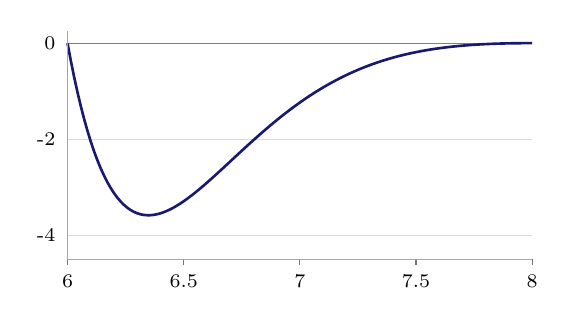
\begin{tikzpicture}[x=1cm,y=1cm,font=\scriptsize]
\draw[black!15] (0,0.3053) -- (5.9,0.3053);
\node[anchor=east] at (-.03,0.3053) {-4};
\draw[black!15] (0,1.5263) -- (5.9,1.5263);
\node[anchor=east] at (-.03,1.5263) {-2};
\draw[black!15] (0,2.7474) -- (5.9,2.7474);
\node[anchor=east] at (-.03,2.7474) {0};
\draw[black!50] (0,2.7474) -- (5.9,2.7474);
\draw[black!55] (0.0000,0) -- +(0,-.065);
\node[anchor=north] at (0.0000,-.07) {6};
\draw[black!55] (1.4750,0) -- +(0,-.065);
\node[anchor=north] at (1.4750,-.07) {6.5};
\draw[black!55] (2.9500,0) -- +(0,-.065);
\node[anchor=north] at (2.9500,-.07) {7};
\draw[black!55] (4.4250,0) -- +(0,-.065);
\node[anchor=north] at (4.4250,-.07) {7.5};
\draw[black!55] (5.9000,0) -- +(0,-.065);
\node[anchor=north] at (5.9000,-.07) {8};
\draw[MidnightBlue,line width=.95pt] plot coordinates {(0.0000,2.7474) (0.0421,2.5233) (0.0843,2.3158) (0.1264,2.1240) (0.1686,1.9471) (0.2107,1.7843) (0.2529,1.6348) (0.2950,1.4981) (0.3371,1.3734) (0.3793,1.2600) (0.4214,1.1574) (0.4636,1.0650) (0.5057,0.9821) (0.5479,0.9084) (0.5900,0.8431) (0.6321,0.7859) (0.6743,0.7363) (0.7164,0.6938) (0.7586,0.6580) (0.8007,0.6284) (0.8429,0.6048) (0.8850,0.5866) (0.9271,0.5736) (0.9693,0.5655) (1.0114,0.5618) (1.0536,0.5623) (1.0957,0.5667) (1.1379,0.5747) (1.1800,0.5860) (1.2221,0.6004) (1.2643,0.6177) (1.3064,0.6376) (1.3486,0.6599) (1.3907,0.6843) (1.4329,0.7108) (1.4750,0.7391) (1.5171,0.7691) (1.5593,0.8005) (1.6014,0.8332) (1.6436,0.8671) (1.6857,0.9020) (1.7279,0.9379) (1.7700,0.9745) (1.8121,1.0118) (1.8543,1.0496) (1.8964,1.0879) (1.9386,1.1265) (1.9807,1.1653) (2.0229,1.2044) (2.0650,1.2435) (2.1071,1.2827) (2.1493,1.3218) (2.1914,1.3608) (2.2336,1.3996) (2.2757,1.4382) (2.3179,1.4765) (2.3600,1.5145) (2.4021,1.5520) (2.4443,1.5892) (2.4864,1.6260) (2.5286,1.6622) (2.5707,1.6979) (2.6129,1.7331) (2.6550,1.7677) (2.6971,1.8018) (2.7393,1.8352) (2.7814,1.8680) (2.8236,1.9001) (2.8657,1.9316) (2.9079,1.9624) (2.9500,1.9925) (2.9921,2.0220) (3.0343,2.0507) (3.0764,2.0788) (3.1186,2.1062) (3.1607,2.1328) (3.2029,2.1588) (3.2450,2.1840) (3.2871,2.2086) (3.3293,2.2324) (3.3714,2.2556) (3.4136,2.2781) (3.4557,2.2999) (3.4979,2.3210) (3.5400,2.3414) (3.5821,2.3612) (3.6243,2.3803) (3.6664,2.3988) (3.7086,2.4166) (3.7507,2.4338) (3.7929,2.4504) (3.8350,2.4664) (3.8771,2.4818) (3.9193,2.4966) (3.9614,2.5108) (4.0036,2.5245) (4.0457,2.5376) (4.0879,2.5502) (4.1300,2.5623) (4.1721,2.5738) (4.2143,2.5848) (4.2564,2.5954) (4.2986,2.6055) (4.3407,2.6151) (4.3829,2.6242) (4.4250,2.6329) (4.4671,2.6412) (4.5093,2.6491) (4.5514,2.6565) (4.5936,2.6636) (4.6357,2.6703) (4.6779,2.6766) (4.7200,2.6826) (4.7621,2.6882) (4.8043,2.6935) (4.8464,2.6985) (4.8886,2.7031) (4.9307,2.7075) (4.9729,2.7116) (5.0150,2.7154) (5.0571,2.7189) (5.0993,2.7221) (5.1414,2.7252) (5.1836,2.7279) (5.2257,2.7305) (5.2679,2.7328) (5.3100,2.7349) (5.3521,2.7369) (5.3943,2.7386) (5.4364,2.7401) (5.4786,2.7415) (5.5207,2.7427) (5.5629,2.7438) (5.6050,2.7447) (5.6471,2.7454) (5.6893,2.7460) (5.7314,2.7465) (5.7736,2.7469) (5.8157,2.7472) (5.8579,2.7473) (5.9000,2.7474)};
\draw[black!35] (0,2.9) -- (0,0) -- (5.9,0);
\end{tikzpicture} &
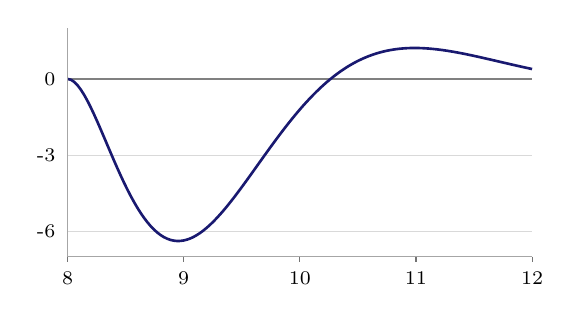
\begin{tikzpicture}[x=1cm,y=1cm,font=\scriptsize]
\draw[black!15] (0,0.3222) -- (5.9,0.3222);
\node[anchor=east] at (-.03,0.3222) {-6};
\draw[black!15] (0,1.2889) -- (5.9,1.2889);
\node[anchor=east] at (-.03,1.2889) {-3};
\draw[black!15] (0,2.2556) -- (5.9,2.2556);
\node[anchor=east] at (-.03,2.2556) {0};
\draw[black!50] (0,2.2556) -- (5.9,2.2556);
\draw[black!55] (0.0000,0) -- +(0,-.065);
\node[anchor=north] at (0.0000,-.07) {8};
\draw[black!55] (1.4750,0) -- +(0,-.065);
\node[anchor=north] at (1.4750,-.07) {9};
\draw[black!55] (2.9500,0) -- +(0,-.065);
\node[anchor=north] at (2.9500,-.07) {10};
\draw[black!55] (4.4250,0) -- +(0,-.065);
\node[anchor=north] at (4.4250,-.07) {11};
\draw[black!55] (5.9000,0) -- +(0,-.065);
\node[anchor=north] at (5.9000,-.07) {12};
\draw[MidnightBlue,line width=.95pt] plot coordinates {(0.0000,2.2556) (0.0421,2.2459) (0.0843,2.2187) (0.1264,2.1762) (0.1686,2.1206) (0.2107,2.0539) (0.2529,1.9780) (0.2950,1.8946) (0.3371,1.8054) (0.3793,1.7117) (0.4214,1.6150) (0.4636,1.5164) (0.5057,1.4171) (0.5479,1.3180) (0.5900,1.2201) (0.6321,1.1242) (0.6743,1.0309) (0.7164,0.9409) (0.7586,0.8547) (0.8007,0.7728) (0.8429,0.6956) (0.8850,0.6235) (0.9271,0.5566) (0.9693,0.4952) (1.0114,0.4395) (1.0536,0.3895) (1.0957,0.3454) (1.1379,0.3072) (1.1800,0.2747) (1.2221,0.2481) (1.2643,0.2273) (1.3064,0.2120) (1.3486,0.2023) (1.3907,0.1979) (1.4329,0.1987) (1.4750,0.2045) (1.5171,0.2151) (1.5593,0.2303) (1.6014,0.2499) (1.6436,0.2737) (1.6857,0.3014) (1.7279,0.3327) (1.7700,0.3675) (1.8121,0.4056) (1.8543,0.4465) (1.8964,0.4903) (1.9386,0.5365) (1.9807,0.5849) (2.0229,0.6354) (2.0650,0.6877) (2.1071,0.7415) (2.1493,0.7967) (2.1914,0.8530) (2.2336,0.9103) (2.2757,0.9683) (2.3179,1.0269) (2.3600,1.0858) (2.4021,1.1449) (2.4443,1.2041) (2.4864,1.2631) (2.5286,1.3219) (2.5707,1.3802) (2.6129,1.4380) (2.6550,1.4951) (2.6971,1.5514) (2.7393,1.6069) (2.7814,1.6613) (2.8236,1.7147) (2.8657,1.7668) (2.9079,1.8178) (2.9500,1.8674) (2.9921,1.9156) (3.0343,1.9624) (3.0764,2.0077) (3.1186,2.0515) (3.1607,2.0938) (3.2029,2.1344) (3.2450,2.1734) (3.2871,2.2109) (3.3293,2.2466) (3.3714,2.2807) (3.4136,2.3132) (3.4557,2.3440) (3.4979,2.3732) (3.5400,2.4008) (3.5821,2.4267) (3.6243,2.4510) (3.6664,2.4737) (3.7086,2.4949) (3.7507,2.5146) (3.7929,2.5327) (3.8350,2.5494) (3.8771,2.5646) (3.9193,2.5784) (3.9614,2.5908) (4.0036,2.6020) (4.0457,2.6118) (4.0879,2.6203) (4.1300,2.6277) (4.1721,2.6339) (4.2143,2.6390) (4.2564,2.6430) (4.2986,2.6459) (4.3407,2.6479) (4.3829,2.6489) (4.4250,2.6490) (4.4671,2.6482) (4.5093,2.6466) (4.5514,2.6443) (4.5936,2.6412) (4.6357,2.6374) (4.6779,2.6330) (4.7200,2.6280) (4.7621,2.6225) (4.8043,2.6164) (4.8464,2.6098) (4.8886,2.6028) (4.9307,2.5953) (4.9729,2.5875) (5.0150,2.5794) (5.0571,2.5709) (5.0993,2.5622) (5.1414,2.5533) (5.1836,2.5441) (5.2257,2.5348) (5.2679,2.5253) (5.3100,2.5157) (5.3521,2.5061) (5.3943,2.4963) (5.4364,2.4865) (5.4786,2.4767) (5.5207,2.4669) (5.5629,2.4571) (5.6050,2.4474) (5.6471,2.4377) (5.6893,2.4281) (5.7314,2.4186) (5.7736,2.4092) (5.8157,2.3999) (5.8579,2.3908) (5.9000,2.3818)};
\draw[black!35] (0,2.9) -- (0,0) -- (5.9,0);
\end{tikzpicture}\\
\multicolumn{2}{c}{Squared physical radius $u$}
\end{tabular}
\end{center}
The curves use the four central frequencies and their interpolation weights. The sign statements use the exact annular densities. The right panel uses a vertical scale one hundred times finer to resolve the positive value past the certified interval.


\subsection{Ten positive spectral weights through squared radius fifteen}
\label{sec:ten-spectral-annuli}
The same explicit spherical-mean construction attains a longer
interval using ten probability densities and the origin bump.
Its physical simple zero is at squared radius $6$; the four
double zeros are at $8,10,12,14$. It is strictly negative on
the rest of $[6,15]$ in squared-radius coordinates. The Fourier
transform is nonnegative, is supported in the ball of radius
$2.27$, and vanishes on neighborhoods of all positive even
squared radii. Both origin values equal one.

Use the bump and radial probability measures of the previous
example, now with $\delta=2^{-180}$. Take the ten phase centres
$t_i$ to be $1/8$ times the integers
$73,74,84,85,94,95,104,105,113,114$.
In the defining matrix use the ten rows corresponding to
$1,K_t(6)$ and the eight numbers $K_t(u),K_t'(u)$ for
$u=8,10,12,14$. The actual weights are again the matrix inverse
applied to the first unit column minus the origin-bump moments.
Their approximate values are as follows. The exact weights are defined by the preceding system.
\begin{center}
\begin{tabular}{r r @{$\qquad$} r r}
\toprule
$8t_i$ & $w_i$ & $8t_i$ & $w_i$ \\
\midrule
73 & 0.0000022150 & 95  & 0.0339248654 \\
74 & 0.0000112534 & 104 & 0.2468095630 \\
84 & 0.0001782268 & 105 & 0.0543437818 \\
85 & 0.0014885506 & 113 & 0.5651716940 \\
94 & 0.0066024669 & 114 & 0.0914673830 \\
\bottomrule
\end{tabular}
\end{center}

For completeness, the degree-$110$ central-phase spherical-mean
approximants to the first three physical jets have error
below $2^{-195}$ on $0\le u\le15$. Replacing a central phase by a
point in its thin interval changes any such jet by less than
$64\delta$; this follows from the derivative formula above,
$|t|<15$, $\sqrt u<4$, and $|\Omega_d|,|\Omega'_d|\le1$.
The polynomial jet matrix has inverse maximum row sum less than
$2^{42}$. Rounding the first column of this inverse to multiples
of $2^{-145}$ and restoring sum one in its last entry leaves a
residual smaller than $2^{-140}$. Each rounded coefficient exceeds
$10^{-6}$ and changes by less than $2^{-95}$ when the actual
smooth spectral measures and the origin bump are used.

Write $h(u)=f(\sqrt u)$ and put $\eta=1/32$.
The exact checker tests $h'<0$ on $[6,6+\eta]$, $h''<0$ on
$[u-\eta,u+\eta]$ about each of the four double nodes, and
$h<0$ on the five intervening or terminal closed intervals.
All ten Bernstein tests pass on their full intervals, with uniform
error below $2^{-87}$. The same rational calculation at squared
radius $18$ gives $f(\sqrt{18})>2.9\cdot10^{-13}$. This last
value exhibits explicitly the eventual failure of the exterior
sign for the ten-weight instance. The standalone replay is
\texttt{ten-shells/verify.py}.


\subsection{How small the positive tail can be}
\label{sec:critical-weight-annulus}
For a radial function $h$ set $\|h\|_\beta=\sup_x(1+|x|)^\beta |h(x)|$. In Theorem~\ref{thm:finite-annulus-polynomial}, for every $\epsilon>0$ the function can in addition be chosen so that
\[
       f(x)\le\epsilon(1+|x|)^{-49/2}\qquad (|x|\ge\sqrt6).
\]
The signed tail lower bound of that theorem still holds. Small pointwise excursions distributed over sufficiently many long shells can carry a fixed positive mass. We give the construction, including the endpoint of the weight estimate.

Fix the polynomial Gaussian seed $H_P$ from the theorem, which is nonpositive on the entire exterior. We claim that the constructed functions can be made arbitrarily close to $H_P$ in $\|\cdot\|_{(d+1)/2}$ while preserving the interpolation conditions. We shall also take errors arbitrarily small through the first two unweighted derivatives.
First cut off the spectral tail of each of the finitely many Gaussian basis functions by a smooth radial cutoff at radius $T$. As $T\to\infty$ the error tends to zero in every Schwartz seminorm on both sides. For fixed $T$ there are now only finitely many positive even spheres to remove from the support. Take disjoint small intervals in radial frequency about their radii.

Write $b=(d-1)/2$. On one such interval about $u_0>0$, let $h_\delta$ be the inverse Fourier transform of $p(\xi)\eta((|\xi|-u_0)/\delta)$, with $p$ any one of the cutoff radial spectra and $\eta$ the even smooth bump equal to one near zero used in the theorem. For $\delta$ sufficiently small one has, uniformly in $r\ge1$,
\[
 |h_\delta(r)|\le C\delta(1+r)^{-b},\qquad
 r^2 |h_\delta(r)|\le C\delta^{-1}(1+r)^{-b}.
\]
Indeed spherical Fourier inversion uses $\Omega_d(2\pi ru)$; on the fixed frequency interval this is $O((1+r)^{-b})$ by the standard Bessel bound $J_{d/2-1}(v)=O(v^{-1/2})$ for $v\ge1$. The first integrand has bounded size on a set of radial length $O(\delta)$. Applying the frequency Laplacian gives the second estimate, since two derivatives cost $O(\delta^{-2})$ and $u$ stays away from zero. On $r\le1$ the first estimate without the decay factor also holds.

Use widths $\delta_j=2^{-j}\delta_0$ and remove the \emph{mean} of these spectral bumps for $1\le j\le M$. This nonnegative multiplier takes value one near $u_0$ and is at most one everywhere. The associated error in $\|\cdot\|_{b+1}$ is $O(1/M)$ since for every $r\ge1$ the sum $\sum_j\min(r\delta_j,(r\delta_j)^{-1})$ is bounded by two geometric series with a uniform bound. Its errors in the first two unweighted physical derivatives also tend to zero by the $O(M^{-1}\sum_j\delta_j)$ weighted spectral mass estimate at this fixed $T$. Perform the operation at each of the finitely many disjoint intervals; the remaining total multiplier is nonnegative and vanishes on every target sphere in the support.

Near frequency zero interpolate to the constant one on a ball of radius $\sigma$. Each added term has the form $p(\xi)\eta_0(\xi/\sigma)$ with $p$ smooth and $\eta_0$ a fixed smooth compactly supported radial cutoff. After scaling, $p(\sigma\cdot)\eta_0$ has uniformly bounded Schwartz seminorms. Its inverse transform therefore has $\|\cdot\|_{b+1}$ norm $O(\sigma^{d-b-1})$, tending to zero for $d>1$. The same scaling gives convergence of the unweighted first two derivatives. These sequential choices approximate each basis vector and the affine constant as closely as desired. Solving the same finite interpolation system again gives coefficients tending to those of $P$, with the same Fourier positivity and physical signs. This proves the assertion.

For this two-sided approximation to the specified seed, the exponent $(d+1)/2$ is sharp. If $\beta>(d+1)/2$, evaluation of the Fourier transform of radial Schwartz functions at any fixed nonzero frequency is a bounded linear functional in $\|\cdot\|_\beta$. This follows by integrating $r^{d-1}(1+r)^{-\beta}|\Omega_d(2\pi r u_0)|$, which is integrable at infinity precisely under the sufficient inequality just stated. The seed has strictly positive transform at the prescribed frequencies, while every approximant vanishes there. This sharpness statement concerns approximation to $H_P$ in the two-sided norm. It leaves open other methods for estimating the positive part alone.

For the functions in the polynomial construction the origin plateau even forces both signs at arbitrarily large radii. Every moment $\int |x|^{2j} f(x)\,dx$ vanishes for $j\ge1$, by differentiation of $\widehat f$ at zero. If $f$ had one weak sign outside a fixed ball, a farther annulus with positive mass of $|f|$ would dominate the whole opposite-sign mass as $j\to\infty$. Such a farther annulus exists because $f$ is real analytic, as the inverse transform of a compact spectrum, and $f(0)=1$.

The same statement holds on the occupied shells of each extremal even unimodular $E$ of rank $48$. For $j\ge1$ apply Poisson summation to $|x|^{2j}f(x)$. All derivatives on the reciprocal side vanish because the spectrum is constant near zero and zero near every other dual node. At $j=0$ the total sum is one and the origin accounts for it. All nonzero physical nodes through $R$ vanish, yielding signed tail sums zero in every one of these moments. An entire function of exponential type that is nonzero at the origin cannot vanish at all sufficiently large radii $\sqrt{2n}$, by Jensen's zero count. Those radii are occupied by $E$. Thus arbitrarily large actual even shells have either sign, by the preceding domination argument.

\paragraph{The required spectral radius.}
If $B_R$ is the radius of a ball supporting the transform of any function of Theorem~\ref{thm:finite-annulus-polynomial}, then $\liminf_{R\to\infty} B_R/R\ge1/(2\sqrt e)$. In fact $g(z)=f(z e_1)$ has $g(0)=1$ and $|g(z)|\le e^{2\pi B_R|\operatorname{Im}z|}$ since $\int\widehat f=1$ and $\widehat f\ge0$. If $m_v$ is its prescribed multiplicity at $v=\sqrt{2j}$, Jensen's formula gives $2\sum_{a\le v\le R}m_v\log(T/v)\le4 B_R T$ for every $T>R$, counting both signs of each zero. Here $a=\sqrt6$. For $T=cR$, $c>1$ fixed, the sum on the left divided by $R^2$ tends to $1+2\log c$ by the elementary Riemann sum over $j/R^2$. Taking $c=\sqrt e$ yields the inequality.

For a one-sided estimate the same dual measure gives a different obstruction at weights above the dimension. For $\beta>48$, the supremum of $(1+r)^\beta f(r)_+$ on $r>R$ is at least $c_\beta R^{\beta-48}$, with $c_\beta>0$ independent of $R\ge\sqrt6$. Indeed $\mu(B_T)\ll T^{48}$ for $T\ge1$: majorize its indicator by $e^\pi e^{-\pi |x|^2/T^2}$, transform the pairing, and use positivity and temperedness of $\widehat\mu$ to bound its integral against $e^{-\pi T^2 |\xi|^2}$ uniformly. Summing dyadic annuli yields $\int_{|x|>R}(1+|x|)^{-\beta}\,d\mu(x)\ll_\beta R^{48-\beta}$. Now apply the positive tail bound $429/25$. The next construction changes the seed and determines the exact borderline for small exterior values.


\subsection{The sharp decay threshold for small exterior values}
\label{sec:annulus-critical-positive}

\begin{theorem}\label{thm:annulus-critical-positive}
For every $R>\sqrt6$ and $\epsilon>0$ the function of
Theorem~\ref{thm:finite-annulus-polynomial} can be chosen to satisfy
$|f(x)|\le\epsilon(1+|x|)^{-48}$ for every $|x|\ge\sqrt6$.
For any fixed $R$, no exponent $\beta>48$ permits arbitrarily small
$\epsilon$ even for the one-sided upper estimate.
\end{theorem}

\begin{proof}
Write $d=48$, $a=\sqrt6$ and
$\|h\|_{d,a}=\sup_{|x|\ge a}(1+|x|)^d|h(x)|$.
We first construct radial high-frequency packets $h$ with all the required
spectral conditions and both normalizations, for which $\|h\|_{d,a}$
and the $C^2$ norm on $a\le |x|\le R$ are arbitrarily small. No
interpolation condition is imposed at the positive physical nodes in this
first step.

Take a smooth nonnegative real $2$-periodic function $\psi$ of mean
one that vanishes in an open neighborhood of $2\mathbb Z$. Write
$\psi(s)=\sum_{k\in\mathbb Z}c_k e^{\pi i k s}$. The coefficients decay
faster than any power and $c_0=1$. For $L\ge1$ consider the nonnegative
spectrum $L^{-d}e^{-\pi|\xi|^2/L^2}\psi(|\xi|^2)$. Its inverse
transform is the absolutely convergent sum $\sum_k c_k A_{k,L}$, where
\begin{equation*}
 A_{k,L}(x)=(1-ikL^2)^{-d/2}
  \exp\!\left(-\frac{\pi L^2|x|^2}{1-ikL^2}\right).
\end{equation*}
The zero mode is $e^{-\pi L^2|x|^2}$. For $k\ne0$, setting $r=|x|$ gives
\begin{equation*}
 |A_{k,L}(x)|\le |k|^{-d/2}L^{-d}
          \exp[-\pi r^2/(2k^2L^2)].
\end{equation*}
Average the spectra for $L_j=2^j L_0$, $1\le j\le M$, and call their
inverse transform $g$. For $r\ge a$, the contribution to
$(1+r)^d|g(x)|$ from $k\ne0$ is at most
\begin{equation*}
 \frac{C_d}{M}\sum_{k\ne0}|c_k|\,|k|^{d/2}
   \sum_{j=1}^M \left(\frac{r}{|k|L_j}\right)^d
        \exp\!\left[-\frac{\pi}{2}\left(\frac{r}{|k|L_j}\right)^2\right].
\end{equation*}
The inner sum is uniformly bounded. Below one its arguments form a
geometric sequence, and above one the Gaussian dominates a negative
power. The zero modes have arbitrarily small exterior norm for large
$L_0$. Also $g(0)=1+O(L_0^{-d})$. On the fixed physical annulus the
nonzero modes, together with their first two Cartesian derivatives,
are $O_R(|k|^{-d/2}L^{-d})$, since
$|L^2/(1-ikL^2)|\le1/|k|$. The zero modes and their derivatives tend
uniformly to zero there. Thus the two smallness requirements follow by
taking $M$ and $L_0$ large.

At fixed $M,L_0$ the averaged spectrum is Schwartz. Multiply it by a
nonnegative smooth radial cutoff that is one up to radius $T$ and zero
beyond $2T$. As $T\to\infty$ this changes its inverse transform by
arbitrarily little in every fixed Schwartz seminorm, hence in both
required norms and at zero. Denote the cutoff spectrum by $p$. It
vanishes near zero as well as near all the positive even squared
frequencies. To supply a plateau at zero, choose a radial smooth
$0\le\eta\le1$ supported in the unit ball and equal to one near zero.
Add the spectrum $u=M^{-1}\sum_{j=1}^M\eta(\xi/\sigma_j)$, where
$\sigma_j=2^{-j}\sigma_0$ and $\sigma_0$ is sufficiently small that
these balls lie in the zero neighborhood of $p$ at the origin and avoid
the first positive prescribed frequency. Its inverse transform is
$M^{-1}\sum_j\sigma_j^d\check\eta(\sigma_j x)$. Since
$|\check\eta(y)|\le C(1+|y|)^{-d-1}$, the same dyadic argument yields
$\|\check u\|_{d,a}=O(1/M)$. Its first two derivatives on the fixed
annulus, and its value at zero, are $O(\sigma_0^d)$ for $\sigma_0\le1$.
Set $\widehat h=u+\gamma p$ with
$\gamma=(1-\int u)/(\int p)$. The two integrals tend to zero and one,
respectively, under the preceding choices. Thus $\gamma>0$ stays bounded,
$h(0)=1$, and $\widehat h$ is one near the frequency origin. This proves
the packet assertion.

Fix a successful index $n$ in the proof of
Theorem~\ref{thm:finite-annulus-polynomial}. Write $F_q=F_{n,q}$ and
let $q_*$ be its exact interpolating polynomial. On a fixed closed
coefficient ball about $q_*$ of sufficiently small positive radius,
$\widehat F_q\ge0$ by strict positivity of all the underlying
Laguerre polynomial coefficients. Every $\widehat F_q$ shares the
required origin plateau and spectral holes, regardless of $h$;
$\|F_q\|_{d,a}\le C$ uniformly on this ball. In particular this family
provides a positivity reserve for all finite-dimensional interpolation
corrections. Its affine sample map $S(F_q)$, comprising the value at zero
and the prescribed positive values and first derivatives, has invertible
linear part. Write $y=(1,0,\ldots,0)$ for the targets.

Choose $0<\lambda<1$ with $\lambda C<\epsilon/2$ and put
$f=\lambda F_q+(1-\lambda)h$. Prescribe
$S(F_q)=y+(1-\lambda)(y-S(h))/\lambda$.
Since $h(0)=1$ and $h$ is arbitrarily small in $C^2$ on the annulus,
this equation has a unique solution arbitrarily close to $q_*$. Thus
$f$ retains spectral nonnegativity and both normalizations. On the
fixed annulus it is arbitrarily close in $C^2$ to $\lambda F_{q_*}$.
Together with exact interpolation, the strict first or second derivative
signs at the prescribed roots and strict negativity elsewhere follow
as in the polynomial proof. Taking $\|h\|_{d,a}<\epsilon/2$ gives the
claimed exterior bound.

Finally, let $a_n$ denote the nonnegative primal masses in the
level-$49$ quadrature of Theorem~\ref{thm:finite-annulus-polynomial},
sampled at $r_n=\sqrt{n/4}$. They satisfy
$\sum_{r_n\le S}a_n=O((1+S)^d)$. For $S\ge1$, apply that quadrature
to $e^{-\pi|x|^2/S^2}$: the left majorizes
$e^{-\pi}\sum_{r_n\le S}a_n$, and on the right the dual Gaussian
sum, after its factor $S^d$ is removed, is bounded by the convergent
corresponding sum at $S=1$, by dual positivity.
Consequently $C_{\beta,R}=\sum_{r_n>R}a_n(1+r_n)^{-\beta}<\infty$
for $\beta>d$, by dyadic summation. The signed tail bound $429/25$
then implies $\epsilon\ge429/(25C_{\beta,R})$ at such an exponent.
\end{proof}

\begin{corollary}\label{cor:annular-doubling-weight}
Let $W:[1,\infty)\to(0,\infty)$ be nondecreasing, with
$W(2s)\le D W(s)$ for all $s\ge1$. At every fixed $R>\sqrt6$,
the exterior majorant in Theorem~\ref{thm:annulus-critical-positive}
for $|f(r)|$ can be replaced by $\epsilon(1+r)^{-48}/W(2+r)$ for arbitrarily small
$\epsilon>0$ if and only if $\sum_{j\ge0}W(2^j)^{-1}$ diverges.
This includes $W(s)=\log(2+s)$.
\end{corollary}
\begin{proof}
Write $\kappa=\log_2 D$, take $L_j=2^j$ and $\sigma_j=2^{-j}$ for
$J\le j\le K$, and assign both spectral averages the weights
$1/(Z W(2^j))$, with $Z=\sum_{j=J}^K 1/W(2^j)$.
For $r\ge a$ the ratio $W(2+r)/W(2^j)$ is bounded by a constant times
$\max(1,(r/2^j)^\kappa)$. In the estimate for the $k$th chirp
this contributes at most $C|k|^{\kappa}\max(1,y^{\kappa})$ with
$y=r/(|k|2^j)$. The dyadic sum of
$y^d e^{-\pi y^2/2}\max(1,y^{\kappa})$ stays uniformly bounded, and
the coefficients $c_k$ absorb the extra polynomial factor in $k$.
The origin estimate uses
$|\check\eta(y)|\le C(1+|y|)^{-d-\kappa-1}$ in the same argument.
Both weighted errors are consequently $O(1/Z)$, apart from the narrow
Gaussian terms, uniformly small for large $J$ since $W$ grows at
most polynomially. First choose $J$ large and then $K$ with $Z$
arbitrarily large. Spectral truncation and the interpolation reserve
continue to apply because the weight has at most polynomial growth.
Conversely, the dyadic mass bound in the preceding proof gives
$\sum_{r_n>R}a_n(1+r_n)^{-d}/W(2+r_n)<\infty$ whenever the reciprocal
series converges. The positive signed tail $429/25$ then precludes
arbitrarily small $\epsilon$.
\end{proof}

In particular one may use $\epsilon/((1+r)^{48}\log(2+r))$, after changing $\epsilon$ by an absolute factor. Replacing the logarithm by its power $1+\eta$ for any $\eta>0$ makes arbitrarily small constants impossible even for an upper bound on $f$ alone. The borderline majorant is still divergent when summed over $48$-dimensional lattice points.

There is a price in the contact slope when the absolute exterior norm tends to zero. Write $g(r)=f(r e_1)$. Positivity and $f(0)=1$ represent $g$ as a probability mixture of $\Omega_{48}(tr)$. Thus $|g''(r)|\le C/a^2$ for $r\ge a$, since $\sup_{u\ge0}u^2|\Omega_{48}''(u)|<\infty$ by the Bessel recurrence and decay. Taylor's inequality, $g(a)=0$ and the absolute exterior bound $\epsilon$ give $|g'(a)|\le\epsilon/h+Ch/(2a^2)$ for $h>0$. The slopes of these arbitrarily flat examples therefore tend to zero. In contrast, if only the first shell contributed to the differentiated Poisson identity on an extremal lattice, the required derivative in the squared-radius variable would be $-4/52\,416\,000$. In the finite-window construction the larger shells contribute to that identity.

\begin{proposition}\label{prop:annulus-volume-defect}
A constant $c>0$ independent of $R$ and $f$ satisfies
$\int_{|x|>R} f_+(x)\,dx\ge c$ for every radial function of
Theorem~\ref{thm:finite-annulus-polynomial}, where $f_+=\max(f,0)$.
\end{proposition}
\begin{proof}
Write $b=2^{1/48}$ and $A=\sum_n a_n e^{-\pi r_n^2}$. Apply the
level-$49$ quadrature to $f(s\cdot)$, $1\le s\le b$, and retain the
dual mass at zero. Then
$\sum_{n\ge24}a_n f(s r_n)\ge(454/25)b^{-48}-1=202/25$.
All $s r_n$ occurring here are at least $\sqrt6$. Upper-bound each
summand by $a_n f_+(s r_n)\mathbf 1_{s r_n>R}$ and integrate in $s$.
After a change of variables the resulting radial density at $r>R$ is
$\sum_{r/b\le r_n\le r,\,n\ge24}a_n/r_n$, bounded above by
$b e^\pi A r^{47}$ by the Gaussian argument above. Thus the assertion
holds with $c=|\mathbb S^{47}|(b-1)(202/25)/(b e^\pi A)$.
\end{proof}

Conversely, with $W(s)=\log(2+s)$ the exterior majorant established
above has finite Lorentz $L^{1,q}$ norm for every $1<q\le\infty$.
Indeed its decreasing rearrangement is bounded by
$C/[(1+t)\log(2+t)]$ at volume parameter $t$. Thus
$\|f_+\mathbf 1_{|x|>R}\|_{L^{1,q}}$ can be made arbitrarily small for
each such $q$, while Proposition~\ref{prop:annulus-volume-defect}
forces its $L^1$ norm to stay bounded away from zero.


\section{A positive right inverse to fibre periodization}
\label{sec:magic-rightinverse}
Let $H,W$ be Euclidean spaces, let $S$ be a full lattice in $H$ of covolume $V$, and write $X=(H/S)\times W$. Give $H/S$ probability Haar measure. A Schwartz function on $X$ is smooth in both variables and rapidly decreasing, with all derivatives, in $W$. Let $\pi:H\times W\to X$ be the quotient. For a closed set $C\subset X$ disjoint from the origin put
\[
 D_C=\pi^{-1}(C)\ \cup\ ((S\setminus\{0\})\times\{0\}).
\]
For a packing of diameter $r$ with horizontal period $S$, the natural choice of $C$ is the set on which $d_S(y)^2+|z|^2\ge r^2$, where $d_S(y)=\min_{s\in S}|y-s|$. Distinct centres have differences in $D_C$, provided centres in the same orbit are also counted. The construction below applies equally to other closed $C$.

\begin{theorem}\label{thm:magic-rightinverse}
There is a linear map $J$ from real even Schwartz functions on $X$ to real even Schwartz functions on $H\times W$ with compact horizontal support, such that $P_SJ=\mathrm{id}$, where $(P_S F)(\bar y,z)=\sum_{s\in S}F(y+s,z)$. It has the following properties for each $b$ with nonnegative Fourier transform:
\begin{enumerate}
\item $\widehat{Jb}\ge0$, $(Jb)(s,0)=b(0)\mathbf1_{s=0}$, and $\widehat{Jb}(0)=V\widehat b(0)$.
\item If $b\le0$ on $C$, then $Jb\le0$ on $D_C$.
\item If $b$ has compact support in the vertical direction, then $Jb$ has compact support.
\end{enumerate}
Consequently, the infimum of $F(0)/\widehat F(0)$ over Euclidean Schwartz tests with sign on $D_C$ and nonnegative Fourier transform equals $V^{-1}$ times the corresponding cylinder infimum for $C$. The infima use tests with positive Fourier value at zero.
\end{theorem}

\begin{proof}
Choose a bounded fundamental cell $D$ for $S$ and a nonnegative $C^\infty$ probability bump $u$ on $H$ with compact support. Put $v=\mathbf1_D*u$ and $\Phi=(v*\widetilde v)/V$, where $\widetilde v(y)=v(-y)$. Then $\Phi,\widehat\Phi\ge0$ and $P_S\Phi=1$. Indeed the $S$-translates of $v$ sum to one, and $\int v=V$. Thus $a_s=\Phi(s)$ is a finitely supported even probability on $S$. Choose nonnegative, even, smooth compactly supported positive definite functions $k$ on $H$ and $h$ on $W$, with $k(0)=h(0)=1$. Normalized autocorrelations of nonnegative bumps suffice. Take their supports sufficiently small that $k(s)=0$ for $s\ne0$ in $S$ and $\pi(\operatorname{supp}k\times\operatorname{supp}h)$ misses $C$. Define
\begin{align*}
 \Psi(y)&=k(y)-\sum_{s\in S}a_sk(y-s),\\
 (Jb)(y,z)&=\Phi(y)b(\bar y,z)+b(0)\Psi(y)h(z).
\end{align*}
The Fourier transform of $\Psi$ is $\widehat k(\xi)\sum_s a_s(1-\cos(2\pi s\cdot\xi))\ge0$, and $P_S\Psi=0$. Thus $P_SJb=b$. Since $\Psi(s)=\mathbf1_{s=0}-a_s$, the claimed samples follow. The Fourier transform of the first term is $\sum_{\lambda\in S^*}\widehat\Phi(\xi-\lambda)\widehat b(\lambda,\eta)$. The hypotheses give absolute convergence and nonnegativity. They also give $b(0)\ge0$ by Fourier inversion. Unfolding $P_SJb=b$ against Haar measure gives the zero-frequency identity. On $\pi^{-1}(C)$ the correction vanishes, since its support projects into the selected neighborhood of zero. The first term there has the sign of $b$ wherever $\Phi>0$. This proves the assertions about $J$.

For the converse let $F$ be any Euclidean feasible test. The cylinder function $b=P_SF$ satisfies $b\le0$ on $C$, $b(0)\le F(0)$, and $\widehat b(\lambda,\eta)=V^{-1}\widehat F(\lambda,\eta)$ for $\lambda\in S^*$. Taking ratios in both directions proves the assertion about the infima.
\end{proof}

The maps on Fourier transforms fit into the commutative diagram
\[
\begin{tikzcd}[column sep=large,row sep=large]
\mathcal S(X) \arrow[r,"J"]\arrow[d,"\mathcal F_X"'] &
\mathcal S(H\times W) \arrow[d,"\mathcal F"]\arrow[l,bend left=20,"P_S"]\\
\mathcal S(S^*\times W) &
\mathcal S(H\times W)\arrow[l,"V^{-1}\mathrm{res}"']
\end{tikzcd}
\]
in the sense that $\mathcal F_XP_S=V^{-1}\mathrm{res}\,\mathcal F$ and $V^{-1}\mathrm{res}\,\mathcal F J=\mathcal F_X$. Periodization of ordinary Euclidean packing tests is treated by A.~Salmon, \emph{Linear programming bounds for fibered sphere packings}, arXiv:2607.25254, Lemma~14. The right inverse above imposes the Euclidean sign on the inverse image of the cylinder constraints together with the nonzero periods. Points whose shortest representative modulo $S$ has length below the exclusion distance can include arbitrarily long Euclidean displacement vectors.


\section{A Schwartz auxiliary function for Leech fibres}
\label{sec:schwartz-leech-fibres}
Write $\mathbb R^{48}=H\mathbin\perp W$ with both summands
of dimension $24$. Normalize the Leech lattice $\Lambda$ to
covolume one and minimum squared length four. Its covering
radius is $\sqrt2$. Let $g$ be the Cohn--Kumar--Miller--Radchenko--Viazovska
Schwartz auxiliary function in dimension $24$ \cite{CKMRV24}, normalized by
$g(0)=\widehat g(0)=1$. Then $\widehat g\ge0$ and $g(z)\le0$
for $|z|\ge2$. Both $g$ and $\widehat g$ vanish at the nonzero
lengths of $\Lambda$. We use the Fourier kernel
$e^{-2\pi i\langle x,\xi\rangle}$.

Fix $S=\sqrt t\,\Lambda\subset H$, with covolume
$V=t^{12}$ and covering radius $R=\sqrt{2t}$. Write $C$
for its closed Voronoi cell, and assume $0<t<3$. Set
$r=\sqrt{6-2t}$. We construct a real Schwartz function
$F_t$ on $H\oplus W$ with
\begin{equation*}
 \widehat F_t\ge0,\qquad F_t(0,0)=1,\qquad
 \widehat F_t(0,0)=V(r/2)^{24},\qquad
 F_t(s,0)=\mathbf 1_{\{0\}}(s)\quad(s\in S).
\end{equation*}
It satisfies $F_t(y,z)\le0$ whenever $|z|\ge r$. The remaining
region where $F_t$ can be positive is bounded, and its horizontal
radius can be taken arbitrarily close to $2R$.

Here are explicit building blocks. For $a>0$ let $u_a$ denote
the radial probability density proportional to
$\exp(-1/(1-|x|^2/a^2))$ for $|x|<a$, continued by zero.
For a real function $w$ write $\widetilde w(x)=w(-x)$.
Fix $\epsilon>0$, take $v=\mathbf1_C*u_\epsilon$ on $H$,
and put $\Phi=v*\widetilde v/V$. Then $\Phi,\widehat\Phi\ge0$,
$\widehat\Phi(0)=V$ and $\operatorname{supp}\Phi
\subset 2C+\overline B_{2\epsilon}$.
The $S$-translates of $v$ sum to one, by convolution of the
almost-everywhere tiling identity for $C$.
Since $\int v=V$, the $S$-translates of $\Phi$ likewise sum
to one. In particular the finitely many numbers $\Phi(s)$,
$s\in S$, give a symmetric probability measure on $S$.

Choose $a>0$ with $2a<\min\{R,\min_{s\ne0}|s|\}$, and choose
$b>0$ with $2b<r$. On $H$ and $W$ respectively use the functions
$k=u_a*\widetilde u_a/\|u_a\|_2^2$ and
$h=u_b*\widetilde u_b/\|u_b\|_2^2$. Both have nonnegative
Fourier transforms and value one at zero.
Define the two terms in the auxiliary function by
\begin{align*}
 \Psi(y)&=k(y)-\sum_{s\in S}\Phi(s)k(y-s),\\
 F_t(y,z)&=\Phi(y)g(2z/r)+\Psi(y)h(z).
\end{align*}
Indeed the Fourier transform of $\Psi$ is $\widehat k(\xi)$
times the finite nonnegative trigonometric polynomial
$\sum_s\Phi(s)(1-\cos(2\pi\langle s,\xi\rangle))$.
In particular $\widehat\Psi$ vanishes on $S^*$.
As $k(s)=\mathbf1_{\{0\}}(s)$ on $S$, one has
$\Psi(s)=\mathbf1_{\{0\}}(s)-\Phi(s)$.
These identities prove the sample conditions and give
\begin{equation*}
 \widehat F_t(\xi,\eta)=(r/2)^{24}\widehat\Phi(\xi)
        \widehat g(r\eta/2)+\widehat\Psi(\xi)\widehat h(\eta)\ge0 .
\end{equation*}
For $|z|\ge r$ the correction vanishes and the first term is
nonpositive on the physical side. For $|y|>2R+2\epsilon$ the
first term vanishes while $k(y)=0$, so that the correction is
nonpositive. Hence the function has a global outer sign past
the radius $\sqrt{(2R+2\epsilon)^2+r^2}$.

\begin{theorem}\label{thm:schwartz-leech-fibres}
A packing of round balls of diameter $\sqrt6$ in dimension $48$
invariant under the translations of $\sqrt t\,\Lambda$ in a
$24$-plane has upper centre density at most
$[4/(t(6-2t))]^{12}$ for $0<t<3$. The auxiliary function $F_t$
has the required pairwise sign on its actual differences and
nonnegative Fourier transform on all of $\mathbb R^{48}$.
At $t=2$ its origin ratio is one. The lattice $P_{48n}$ has
such an involution fixed lattice \cite[Theorem~4.10 and Table~2]{Nebe48}.
All extremal unimodular
lattices containing this horizontal period lattice attain the
bound and saturate its Poisson identity.
\end{theorem}
\begin{proof}
At any occupied vertical coordinate the horizontal fibre is a
union of cosets of $S$. It is exactly one coset: two different
cosets in that fibre would have representatives at distance at
most $R<\sqrt6$. For any two distinct occupied vertical
coordinates, representatives of their two horizontal cosets
can be chosen at horizontal distance at most $R$.
Thus their vertical separation is at least
$\sqrt{6-R^2}=r$, even when the shifts of different layers are
unrelated. Differences within a layer belong to $S\times\{0\}$,
where all nonzero values of $F_t$ vanish. Differences between
layers have $|z|\ge r$, where $F_t\le0$.

The usual Fourier packing bound now applies, giving inverse
origin ratio $\widehat F_t(0)/F_t(0)=V(r/2)^{24}$ as the
minimum volume per centre. For a periodic set this follows by
Poisson summation of its difference multiset. For arbitrary
layer arrangements, one can equivalently apply the
$24$-dimensional bound to the $r$-separated set of vertical
coordinates. Each horizontal fibre is a translate of $S$, whose
count in expanding cubes is $V^{-1}$ times their volume, up to
a uniform boundary error. This gives the same upper centre
density without a vertical periodicity assumption. Alternatively
one may periodize finite patches with a buffer exceeding the
global outer-sign radius just proved, and let the cube size tend
to infinity. At $t=2$ equality in the Poisson bound forces the
vanishing of every nonzero physical and reciprocal term for an
attaining lattice, by their respective signs.
\end{proof}

For $t=2$, the finite Fourier correction can use only the three
nonzero horizontal squared lengths $8,12,16$: take
$4+2\epsilon<\sqrt{20}$ and use the even norms of $\Lambda$.
The resulting function also certifies arbitrary configurations
whose differences have either $|z|\ge\sqrt2$ or $z=0$, $y\in S$.
The sign in the shorter vertical interval requires this geometric
information or direct testing of the displayed formula. Thus it
is a sharp, nonradial Schwartz auxiliary function for a class of
rank-$48$ packings.


\subsection{A displacement at which the Leech-fibre test is positive}
\label{sec:fibre-positive-example}
The failure of the unrestricted sign is explicit, including on a rotated copy of the attaining lattice. In the construction at $t=2$, take $\operatorname{supp}k\subset B_{1/10}(0)$. Then
\[
                F_2(y,0)>0\qquad(y\in H,\ |y|=\sqrt6).
\]
Indeed $S=\sqrt2\Lambda$ has shortest length $\sqrt8$. Hence every such $y$ is at distance at least $\min(\sqrt6,\sqrt8-\sqrt6)>1/10$ from $S$. All summands of $\Psi$ vanish at $y$. The Voronoi cell $C$ contains the ball of radius $\sqrt2$, so $C$ and $C+y$ overlap on an open ball when $|y|=\sqrt6<2\sqrt2$. Using $v=\mathbf1_C*u_\epsilon$ with $u_\epsilon$ positive near zero, $v$ is positive on the interior of $C$, and consequently $\Phi(y)>0$. Since $g(0)=1$, the assertion follows. Rotate $P_{48n}$ so that a shortest vector points in this direction. Its minimum and covolume are unchanged, while this one shortest-vector term now has positive value. This calculation precisely identifies a sign that a proof for arbitrary lattices would have to replace or compensate.


\subsection{\texorpdfstring{A saturated Schwartz function for Nebe's $72$-dimensional lattice}{A saturated Schwartz function for Nebe's 72-dimensional lattice}}
\label{sec:nebe-fibre-magic}
Split $\mathbb R^{72}=H_1\perp H_2\perp H_3$ into three
$24$-planes. A diameter-$\sqrt8$ packing with horizontal periods
$S_1\cong\sqrt2\,\Lambda$ in $H_1$ projects to a packing of
diameter at least two in $H_2\oplus H_3$, by the first-layer
argument just given. Suppose this projection has periods
$S_2\cong\Lambda$ in $H_2$. Its projection to $H_3$ then has
separation at least $\sqrt2$. The density of centres in
$\mathbb R^{72}$ is at most one. There is one real Schwartz
auxiliary function realizing this bound on these configurations,
with nonnegative Fourier transform everywhere.

For its formula, form $\Phi_i,\Psi_i$ from $S_i$ as above,
using the corresponding covolume $V_i$. Put
$T(y_2,z)=\Phi_2(y_2)g(\sqrt2 z)+\Psi_2(y_2)h_2(z)$,
with $h_2(0)=1$ and $\operatorname{supp}h_2\subset B_{\sqrt2}$.
In the same construction choose $h_1$ on $H_2\oplus H_3$ with
$h_1(0)=1$, $\widehat h_1\ge0$ and support in $B_2$. Then
\begin{equation*}
 F(y_1,y_2,z)=\Phi_1(y_1)T(y_2,z)+\Psi_1(y_1)h_1(y_2,z).
\end{equation*}
It has $F(0)=1$ and
$\widehat F(0)=V_1 V_2\,2^{-12}=2^{12}\cdot1\cdot2^{-12}=1$.
Both terms have nonnegative Fourier transforms. A nonzero difference
within a first-layer fibre has sample zero. Otherwise the projected
difference has length at least two, which removes the last correction.
The inner function is nonpositive on that projected difference,
by the same within-layer and between-layer argument. These statements
also hold when different fibres are translated independently,
provided the stated diameters hold.

Nebe's extremal unimodular lattice $\Gamma$ has exactly this flag.
In her polarization description, $M+N=\Lambda$,
$M\cap N=2\Lambda$ and $M/\sqrt2\cong\Lambda$. In the ordinary
Leech metric the vectors of $\Gamma$ are
$(w+x,w+y,w+z)/\sqrt2$ with $w\in N$, $x,y,z\in M$ and
$x+y+z\in2\Lambda$ \cite[Section~2]{Nebe72}. The pure first
coordinate is $2\Lambda/\sqrt2$: indeed $w+y=w+z=0$ forces
$w\in2\Lambda$ and then $w+x\in2\Lambda$, and every such
coordinate occurs. In the projection to the last two coordinates
the pure second coordinate is $M/\sqrt2$. The condition
$w+z=0$ forces $w\in2\Lambda$; conversely take
$(w,x,y,z)=(0,-y,y,0)$ for any $y\in M$.
Finally the projection to the last coordinate is
$(M+N)/\sqrt2=\Lambda/\sqrt2$. Thus $\Gamma$ attains the
bound. By Poisson summation all the nonzero samples of $F$ on
$\Gamma$ and of $\widehat F$ on $\Gamma^*$ vanish.


\section{A compactly supported function for every primitive hyperplane flag}
\label{sec:compact-magic-flag}
We construct an ambient function adapted to each extremal lattice, including those for which no rank-$24$ Leech section has been identified. Its allowed displacements have a gap in a single fixed direction. We give the one-dimensional factor explicitly so that every physical support in this construction can be bounded.

\begin{lemma}\label{lem:magic-one}
For each $0<\rho<1/4$ there exists a real even function $g\in C_c^\infty(\mathbb R)$ with $\widehat g\ge0$, $g(0)=\widehat g(0)=1$, $g(n)=\mathbf1_{n=0}$ on $\mathbb Z$, and $g(x)\le0$ when $|x|\ge1$. Its support lies in $[-1-\rho,1+\rho]$.
\end{lemma}
\begin{proof}
Write $T(x)=(1-|x|)_+$. Choose an even, nonnegative, positive definite smooth function $k$ supported in $[-\rho,\rho]$ with $k(0)=1$, for example a normalized bump autocorrelation. Choose $0<\delta<\rho$ with $\delta^2\|k''\|_\infty\le2$, and let $b$ be an even nonnegative smooth probability autocorrelation supported in $[-\delta,\delta]$. Put $A=T*b$ and $c=A(1)$. Take
\[
   g(x)=A(x)+c\{2k(x)-k(x-1)-k(x+1)\}.
\]
All integer translates of $T$ sum to one. Hence $A(0)+2c=1$, since $A$ vanishes on integers of absolute value at least two. This proves the cardinal values and $\widehat g(0)=1$. Both Fourier summands are nonnegative: $\widehat T$ is the square of a sinc, and the correction multiplier is $2c(1-\cos(2\pi\xi))$. For $0\le t\le\delta$ the expression $A(1+t)=\int_t^\delta (s-t)b(s)\,ds$ is convex and lies below $c(1-t/\delta)$. Taylor's inequality gives $k(t)\ge1-\|k''\|_\infty t^2/2\ge1-t/\delta$. Thus $g(1+t)\le0$ in this interval. Beyond it $A(1+t)=0$ and the only possible term is $-ck(t)$. Evenness and the supports finish the proof.
\end{proof}

Let $E$ be any covolume-one lattice of dimension $d\ge2$. Choose a primitive dual vector $w\in E^*$, put $H=w^\perp$, $S=E\cap H$, and let $a=1/|w|$. The homomorphism $x\mapsto w\cdot x$ on $E$ is onto $\mathbb Z$, so $E$ has heights $a\mathbb Z$ and its horizontal section has covolume $1/a$. In Theorem~\ref{thm:magic-rightinverse} take $b(\bar y,z)=g(z/a)$ and use $C=\{|z|\ge a\}$. The resulting function $F$ is smooth with compact support in $\mathbb R^d$ and satisfies
\[
 F(0)=\widehat F(0)=1,\qquad \widehat F\ge0,\qquad
 F(s,0)=\mathbf1_{s=0},\qquad F(y,z)\le0\quad (|z|\ge a).
\]
It has the full lattice-node zeros on $E$ and $E^*$ by Poisson summation and positivity. Moreover the ambient centre intensity bound one holds for any collection of single $S$-cosets at heights mutually separated by at least $a$. Their offsets can vary independently, as can the successive spacings above their common lower bound. In fact the same bound holds for any point set with all nonzero differences in $D_C$. For finite patches, periodic repetition with a buffer larger than the support of $F$ proves the assertion by the usual Fourier packing bound, followed by the large-cube limit.

In rank $48$ choose any shortest $w$ of an extremal even unimodular $E$. Then $a=1/\sqrt6$. The unit intensity is attained at minimum $\sqrt6$ by $E$ itself. It is essential to impose the height and horizontal constraints: in the unrestricted problem an oblique displacement of length $\sqrt6$ can have arbitrarily small nonzero height. The construction alone gives no sign there. More generally it applies verbatim to any existing extremal even unimodular lattice in rank $24n$, with $a=(2n+2)^{-1/2}$ for a shortest $w$. The geometric theorem on hyperplane layers in Section~\ref{sec:lamination} yields examples of offset restrictions in dimension $48$ for which the hard-sphere condition itself implies this height gap.


\subsection{An evaluable formula in forty-seven basis coordinates}
\label{sec:flag-coordinates}
For the hyperplane construction one can avoid computing a Voronoi cell, or summing over its neighboring lattice points. Let $B$ be any horizontal basis matrix for the section. In Lemma~\ref{lem:magic-one} write $A=T*b$, $c=A(1)$, and reuse the same $k$ and $g$. For $u=B^{-1}y$ and $v=z/a$ put $K_c(t)=c k(t-1)+(1-2c)k(t)+c k(t+1)$. The following is a single function on the ambient Euclidean space, written in adapted coordinates:
\[
 F(Bu,av)=g(v)\prod_{i=1}^{d-1}A(u_i)
       +k(v)\left\{\prod_{i=1}^{d-1}k(u_i)-\prod_{i=1}^{d-1}K_c(u_i)\right\}.
\]
Indeed $\Phi(Bu)=\prod_iA(u_i)$ is nonnegative, has nonnegative Fourier transform and periodizes to one. The samples $A(n)$ are $c,1-2c,c$ at $n=-1,0,1$ and zero elsewhere. This gives the displayed product for the convolution of its sample probabilities with $\prod_i k$. Thus evaluation takes linearly many one-dimensional operations. At integer $u$ and integer $v$ it has the required zero samples when $v\ne0$ or $u\ne0$; more generally, at every nonzero integer $v$ it vanishes identically for all $u$. The target-space proof applies just as well when the projected heights are nonintegral and mutually separated by at least $a$.

The accompanying implementation evaluates the displayed function with smooth bump autocorrelations. A second implementation uses a centred even-order cardinal spline, whose Fourier transform is an even power of a sinc. This latter implementation provides exact rational checks of physical values and has finite differentiability. The smooth construction is the one in the theorem.

For the smooth numerical realization one may use $u(t)=\exp(-1/(1-4t^2))$ on $|t|<1/2$, zero elsewhere. Write $I=u*\widetilde u$, take $k(t)=I(t/\rho)/I(0)$ and $b(t)=I(t/\delta)/(\delta(\int u)^2)$ with $\rho=1/8$, $\delta=\rho/64$. Integration by parts gives $\rho^2\|k''\|_\infty\le\|u'\|_2^2/\|u\|_2^2<900$, since $\|u'\|_\infty\le16/e^2<3$ and $\|u\|_2^2\ge e^{-8/3}/2>1/100$. This verifies the curvature condition of the lemma directly. For the rational realization use the density of the sum of eight independent uniform variables on $[-1/8,1/8]$ in place of $I$, with the same normalizations. Its maximum is at zero and is at least $1/2$. Twice differentiating the convolution gives a second difference of the six-factor density divided by $(1/4)^2$, of absolute value at most $4/(1/4)^3$. The curvature condition follows here as well.


\section{\texorpdfstring{A finite tube obstruction for arbitrary rank-$48$ lattices}{A finite tube obstruction for arbitrary rank-48 lattices}}
\label{sec:finite-leech-tubes}
\begin{theorem}
Let $L$ be any lattice in $\mathbb R^{48}$ with squared minimum at
least six and covolume at most one. For every orthogonal splitting
$H\perp W$ into $24$-planes there are at least $2\,616$ signed
nonzero vectors $x=(y,z)\in L$ such that
$|y|^2<32/3$, $|z|^2<10/3$ and $|x|^2<14$.
They give at least $1\,308$ distinct unoriented lines. More precisely,
for any orientation of the Leech lattice in $H$ one may require
$y\in\operatorname{int}(2C)$, where $C$ is the Voronoi cell of
$\sqrt{4/3}\,\Lambda$ in that orientation.
\end{theorem}
\begin{proof}
Use the Schwartz lift with $t=4/3$. Thus $R^2=8/3$, $r^2=10/3$,
and Poisson summation gives
$\sum_{x\ne0}F_t(x)\ge A$, where $A=(10/9)^{12}-1$.
For $0<|x|$ and $|z|<r$ the minimum condition gives
$|y|^2\ge6-|z|^2>R^2$. Therefore $k(y)=0$ and $\Psi(y)h(z)\le0$.
For $|z|\ge r$ the whole summand is already nonpositive.
Letting $\epsilon\downarrow0$ in the resulting upper estimate on
$\sum_{x\ne0}F_t(x)$ yields
\begin{equation*}
 A\le\sum_{\substack{0\ne (y,z)\in L\\ |z|<r}}
 c_C(y)\max\{g(2z/r),0\},\qquad
 c_C(y)=\frac{\operatorname{vol}(C\cap(C+y))}{t^{12}}.
\end{equation*}
Indeed the smoothed covariograms converge uniformly to $c_C$,
by continuity of the compactly supported covariogram and convolution
with an approximate identity. For all sufficiently small $\epsilon$
a single compact cylinder contains the support of every positive
summand. The covariogram is positive only for
$y\in\operatorname{int}(C-C)=\operatorname{int}(2C)$, so every
positive summand meets the three claimed strict cutoffs.

To bound each summand, let $s=2|z|/r$. If a sphere of radius $s$
in $24$-space contains $N$ points at mutual distances at least
two, then $|g(s)|\le N^{-1/2}$. In fact positive definiteness and
the Cauchy--Schwarz inequality for its Gram matrix give
$N^2g(s)^2\le g(0)\sum_{i,j}g(u_i-u_j)\le N$.
A code at any smaller radius remains admissible after dilation.
Regular simplices supply $N=k$ at squared radius $2(k-1)/k$ for
$2\le k\le24$. The cross polytope supplies $48$ points at squared
radius two. Three further squared-radius thresholds and cardinalities
are $(63/25,96)$, $(8/3,304)$ and $(3,4144)$.

For the first, use the signed coordinate basis and the signed
rows of a Hadamard matrix of order $24$, normalized to unit length.
Their largest mutual inner product is $1/\sqrt{24}\le1-50/63$.
For the second, the signed coordinate basis in $24$ dimensions
is joined by $256$ sign vectors on the first $16$ coordinates.
Write those coordinates as $i\in\mathbb F_2^4$. The signs are
$(-1)^{q(i)+a\cdot i+c}$, with arbitrary $a,c$ and with the six
quadratic cross-term coefficients of $q$ given as a binary mask
in lexicographic pair order, the first pair taking the lowest bit.
The masks are $0,12,22,27,39,41,53,58$. All distinct sign vectors
differ in at least six positions, so after normalization the largest
mutual inner product is $1/4$. For the last code adjoin the $4096$
sign vectors of the extended binary Golay code to the $48$ signed
coordinates. Its minimum distance is eight and its largest normalized
inner product is at most $1/3$. The accompanying program constructs
the Hadamard matrix from the quadratic residues modulo $23$ and
checks both binary distance calculations directly.

Since $C\subset B_R$, the intersection of the two Voronoi cells
lies in the intersection of two balls of radius $R$. Slicing
that intersection perpendicular to $y$ gives
\begin{equation*}
 c_C(y)\le 2^{13}v_{23}\int_{|y|/(2R)}^1(1-u^2)^{23/2}\,du ,
 \qquad v_{23}=4^{12}12!\pi^{11}/24!.
\end{equation*}
On an interval of values of $s$ ending at $s_1$, the lower endpoint
in this integral is at least $\sqrt{(6-5s_1^2/6)/(32/3)}$.
Use the code at the left endpoint of the interval for $N$, with
$N=1$ on the first interval; the final right endpoint is $s_1=2$.
The $28$ resulting upper bounds on $c_C(y)|g(s)|$ are all
strictly less than $A/2614$.

For a reproducible rational check let $m=65536$, let $a$ be the
square root in the previous paragraph and put $j_0=\lfloor ma\rfloor$.
An upper bound for the integral is
$m^{-24}\sum_{j=j_0}^{m-1}(m^2-j^2)^{11}
\lceil\sqrt{m^2-j^2}\rceil$.
This is a left Riemann sum with each square root rounded upward.
Use $\pi<355/113$, which the program verifies with alternating
arctangent series, and square the comparison to remove $\sqrt N$.
Consequently more than $2614$ positive summands are necessary.
They occur in opposite pairs, and lengths below $\sqrt{14}$ admit
no two different positive integer multiples on the same lattice line
because $2\sqrt6>\sqrt{14}$. This proves the assertion.
\end{proof}


\subsection{A spectral sharpening of the tube bound}
The spherical Fourier representation and the zero $g(2)=0$
raise the preceding bound to $14\,252$ signed vectors with
$|y|^2<32/3$, $|z|^2<10/3$, $|x|^2<14$. A second choice of the
scale gives at least $15\,002$ signed vectors satisfying
$|y|^2<10$, $|z|^2<7/2$, $|x|^2<27/2$, in every such splitting.
Each antipodal pair again contributes one line.
These statements require only the same lattice hypotheses.

Let $\Omega_d(u)$ be the average of $\cos(u\theta_1)$ over the unit
sphere in $d$ dimensions. Fourier inversion gives
$g(s)=\int_0^\infty\Omega_{24}(s v)\,d\mu(v)$, where $\mu$
is the probability measure obtained from
$\widehat g(\xi)\,d\xi$ under $v=2\pi|\xi|$. In particular
$\int\Omega_{24}(2v)\,d\mu(v)=0$.
Write $Y=\Omega_{24}$. For $q$ in $[0,16]$ the function $Y(q)$ is
nonincreasing, and $|Y(q)|<1/1600$ for $q\ge16$.
For a verification, expand the spherical cosine mean in powers of
$q^2$. Its consecutive term ratio in dimension $d$ is
$-q^2/(2(j+1)(d+2j))$, beginning with one at $j=0$. Truncation
after an even index gives an upper bound, and after an odd index
a lower bound, by the corresponding global Taylor bounds for
cosine. This verifies $\Omega_{26}\ge0$ through $16$ and
$Y(16)^2+Y'(16)^2<1600^{-2}$ by rational polynomial arithmetic.
The same series gives $Y'(q)=-(q/24)\Omega_{26}(q)$ and
$Y''+(23/q)Y'+Y=0$. Consequently the energy $Y^2+(Y')^2$ is
nonincreasing, as required.

Consider either $(t,N)=(4/3,14250)$ or $(5/4,15000)$ and set
$A=(t(6-2t)/4)^{12}-1$. For each interval $[a,b]$ with
$a=j/40$, $b=(j+1)/40$, $24\le j<80$, the certificate gives a
nonnegative rational coefficient $c$ and an upper bound $B$.
It verifies
\begin{equation*}
 Y(av)-cY(2v)\le B\quad(0\le v\le16/a),\qquad (1+c)/1600<B .
\end{equation*}
For $a\le s\le b$, the same bound holds with $Y(sv)$ in place
of $Y(av)$ and all $v\ge0$. Indeed if both arguments lie below
$16$ this follows by monotonicity. If $sv\ge16$, use
$Y(sv)\le1/1600$ and $Y(2v)\ge-1/1600$, the latter following
from the monotonicity and the energy bound together. Integration
against $\mu$ therefore gives $g(s)\le B$.

For $s\le b$ the horizontal overlap factor is bounded by
$J_t(b)=2^{13}v_{23}\int_{a_t(b)}^1(1-u^2)^{23/2}\,du$,
where $a_t(b)^2=(6-(6-2t)b^2/4)/(8t)$. The verifier uses the
previous rational Riemann sum to majorize $J_t(b)$, and chooses
$B$ by rounding down $A$ divided by $N$ times that majorant
to a multiple of $10^{-7}$. For the interval $[0,3/5]$,
$|g(s)|\le1$ alone suffices. In all intervals the resulting
upper cost of a summand is strictly below $A/N$; the Riemann
bound for the integral is strict. For the first polynomial
comparison use the degree-$80$ upper truncation of $Y(av)$ and
the degree-$81$ lower truncation of $Y(2v)$ as polynomials in
$v^2$. Affinely normalize $0\le v^2\le(16/a)^2$ to $[0,1]$
and test the difference by exact Bernstein coefficients and
dyadic subdivision. The checks take $90$ and $85$ terminal
intervals, respectively. The program \texttt{spectral.py}
reproduces every comparison. The Poisson inequality and parity
of the signed count finish both cases.

The $15\,002$ vectors in the second tube span a space of dimension
at least ten. To see this, take the rank-$q$ lattice obtained by
intersecting their real span with $L$. Each vector has length
strictly below $3\sqrt6/2$, so the zero residue class modulo twice
this lattice is absent. In a given nonzero class two vectors
$u,v$ on distinct lines have both $(u+v)/2$ and $(u-v)/2$
nonzero in $L$. With $a=|u|/\sqrt6$ and $b=|v|/\sqrt6$, the
absolute cosine between the lines is at most
$(a^2+b^2-4)/(2ab)<1/9$. Indeed this expression increases in
each variable on $[1,3/2]^2$ and equals $1/9$ at $(3/2,3/2)$.
If there are $m$ such lines, their unit representatives have a
Gram matrix with trace $m$, rank at most $q$, and squared
Frobenius norm at most $m+m(m-1)/81$. Cauchy--Schwarz gives
$m\le80q/(81-q)$ for $q<81$. At $q\le9$ there would consequently
be at most $2(2^9-1)\lfloor80\cdot9/72\rfloor=10\,220$
signed vectors, contradicting the count.


\section{Positive Fourier interpolation of contact gradients}
\label{sec:cardinal-first-jets}
Let $E$ be a Euclidean lattice of covolume one in dimension $d$.
A cardinal function for $E$ takes value one at zero and zero at all other
points of $E$. Write $uv^{\mathsf T}$ for the outer product of column vectors.

\begin{theorem}\label{thm:cardinal-jets}
Suppose $g_v\in\mathbb R^d$ for $v\in E$ is a finitely supported odd family.
There exists a real even Schwartz function $f$ with the following properties
if and only if $\sum_{v\in E}g_vv^{\mathsf T}=-I$:
\begin{enumerate}
\item $f$ and $\widehat f$ are cardinal for $E$ and $E^*$, respectively.
\item $\widehat f$ is nonnegative, smooth and compactly supported.
\item $\nabla f(v)=g_v$ for every $v\in E$.
\end{enumerate}
\end{theorem}
\begin{proof}
For necessity put $p=\widehat f$ and form the $E^*$-periodic vector
$m(\xi)=\sum_{\lambda\in E^*}(\xi+\lambda)p(\xi+\lambda)$.
At each nonzero $\lambda\in E^*$ the nonnegative function $p$ and its
gradient vanish, so $Dm(0)=I$. Its Fourier coefficient of index $-v$ is $g_v/(2\pi i)$ by unfolding.
Differentiation of this finite Fourier series gives the asserted condition.

Conversely, define the real odd trigonometric polynomial $m$ by these
Fourier coefficients. Thus $Dm(0)=I$. Choose a basis matrix $B$ for $E$. In the coordinates
$y=B^{\mathsf T}\xi$ set $M(y)=B^{\mathsf T}m(B^{-\mathsf T}y)$ and
$q(y)=M(y)-y$. Then $q(y+k)=q(y)-k$ for $k\in\mathbb Z^d$ and
$q(y)=O(|y|^3)$ at the origin. We construct a nonnegative even
$P\in C_c^\infty(\mathbb R^d)$ satisfying
\begin{equation}\label{eq:cardinal-lift}
 \sum_{k\in\mathbb Z^d}P(y+k)=1,\qquad
 \sum_{k\in\mathbb Z^d}(y+k)P(y+k)=M(y).
\end{equation}
For an explicit preliminary lift take a smooth, even, nonnegative
one-dimensional bump $b$ supported on $[-1/8,1/8]$ with integral one,
and put $\phi=(1-|\cdot|)_+*b$. Linear interpolation on an interval, followed
by integration against $b$, gives $\sum_j\phi(u-j)=1$ and
$\sum_j j\phi(u-j)=u$. Therefore $P_1(y)=\prod_i\phi(q_i(y))$ satisfies
\eqref{eq:cardinal-lift}. Its support is compact since $M$ is bounded.

To impose cardinality, choose $0<r<1/4$ so small that $2dr^2<1$
and $|q_i(z)|\le 2|z|^2$ when $|z|<r$. On disjoint open balls around
integers write $y=z+k$, $|z|<r$, and assign
\begin{align*}
 P_0(z)&=1-2d|z|^2, &P_0(z\pm e_i)&=|z|^2\pm q_i(z)/2.
\end{align*}
Assign value zero at every other translate of this ball. The weights are
nonnegative, sum to one, and have mean displacement $q(z)$, proving
\eqref{eq:cardinal-lift} locally. Take a periodic even smooth cutoff $\chi$
supported in the open balls and equal to one on the balls of radius $r/2$.
Then $P=\chi P_0+(1-\chi)P_1$ is smooth, compactly supported, even and
nonnegative. It satisfies both identities because the cutoff is periodic.
At integer points it is cardinal. One may take $r$ directly from the
third-derivative bound for the displayed trigonometric polynomial.

Set $p(\xi)=P(B^{\mathsf T}\xi)$ and $f=\mathcal F^{-1}p$. Unfolding the
first identity in \eqref{eq:cardinal-lift} gives $f(v)=\mathbf1_{v=0}$,
using $|\det B|=1$. The second identifies $\nabla f(v)/(2\pi i)$ with the Fourier coefficient
of $m$ at $-v$, hence $\nabla f(v)=g_v$. The inverse transform of $p$ is real, even, entire of
exponential type, and Schwartz on $\mathbb R^d$.
\end{proof}

Let $S$ contain one vector from each pair of shortest vectors of $E$.
Theorem~\ref{thm:cardinal-jets} gives a Fourier characterization of
strict eutaxy. A positive eutaxy identity $\sum_{v\in S}a_vvv^{\mathsf T}=I$
is equivalent to having the cardinal function above with gradients
$-a_vv/2$ on $S$, positive $a_v$, the gradients on $-S$ given by oddness,
and zero gradients everywhere else on $E$. The prescribed first moment
in this case has the especially simple form
$m(\xi)=(2\pi)^{-1}\sum_{v\in S}a_vv\sin(2\pi\langle v,\xi\rangle)$.
If desired the stabilizer of $E$ may be imposed on the construction by
averaging it, using invariant eutaxy weights.

\begin{corollary}\label{cor:local-cardinal-jets}
For a perfect, strictly eutactic $E$, this function gives a sharp
lattice-summed inequality in a neighborhood of $E$ in the space of lattices
modulo rotations. For positive definite symmetric $A$ sufficiently close
to $I$, if $m(AE)\ge m(E)$ then $\sum_{v\in E\setminus\{0\}}f(Av)\le0$,
with strict inequality for $A\ne I$. Rotating the test by the orthogonal
factor of a general basis change supplies the equivalent statement for an
arbitrary orientation.
\end{corollary}
\begin{proof}
Put $J=A^2-I$ and take the Frobenius norm. The minimum assumption gives
$v^{\mathsf T}Jv\ge0$ on $S$. The cone has a positive constant
$\gamma=\min\{\operatorname{tr}D:\|D\|_F=1,\;v^{\mathsf T}Dv\ge0
\text{ for }v\in S\}$. Indeed, zero trace would force every contact
quadratic to vanish by strict eutaxy, and then $D=0$ by perfection.
For $\|J\|_F\le1/2$, the scalar inequality $\log(1+t)\ge t-t^2$
gives $\det A\ge1+(\gamma\|J\|_F-\|J\|_F^2)/2$.

Choose $R$ enclosing the support of $p$ and let $K=\sup_\xi\|D^2p(\xi)\|_{\rm op}$.
Only $\lambda\in E^*$ with $|\lambda|\le2R$ can contribute to the Poisson
sum. Since $\|A^{-1}-I\|_{\rm op}\le2\|J\|_F$ and $p$ has a double zero
at every nonzero $\lambda\in E^*$, the sum of its nonzero dual terms
is at most $2KH\|J\|_F^2$, where
$H=\sum_{\lambda\in E^*,\,0<|\lambda|\le2R}|\lambda|^2$.
Consequently a sufficient window is
$0<\|J\|_F<\min\{1/2,\gamma/(1+4KH)\}$.
Poisson gives the strict asserted sign. At $A=I$ it is equality by cardinality.
The first variation is concentrated entirely on the minimal vectors:
$\sum_{v\in E}\nabla f(v)^{\mathsf T}Dv=-\operatorname{tr}D$.
\end{proof}
For a spherical $4$-design of shortest vectors, the usual second and
fourth moments give the explicit choice
$\gamma\ge[(d+2)-\sqrt{(d+2)^2-8}]/2$. Indeed for
$Y=v^{\mathsf T}Dv\ge0$ and $\|D\|_F=1$ one has
$Y^2\le|v|^2Y$. Taking the two moments yields
$2+(\operatorname{tr}D)^2\le(d+2)\operatorname{tr}D$.
For an extremal rank-$48$ lattice the coefficients in the eutaxy identity
are all equal to $48/(6\cdot26208000)$, so the finite sine polynomial
is determined by the minimal vectors alone.


\subsection{Arbitrarily flat dual zeros from multiples of the contacts}
\label{sec:cardinal-flat}
Suppose $\sum_{v\in S}a_vvv^{\mathsf T}=I$ with $a_v>0$, as above. For an
integer $k\ge1$, put
\begin{equation*}
 D_k(t)=\sum_{j=1}^k d_{k,j}\sin(jt),\qquad
 d_{k,j}=\frac{2(-1)^{j+1}(k!)^2}{j(k-j)!(k+j)!}.
\end{equation*}
Then $D_k(t)=t+O(t^{2k+1})$. Indeed the centered interpolation formula
for the derivative at zero on $-k,\ldots,k$ has coefficient $d_{k,j}/2$
at $j>0$ and its negative at $-j$. This follows by differentiating the
Lagrange basis polynomial at zero. Exactness on monomials of degree
through $2k$ proves the asserted Taylor formula.

\begin{proposition}\label{prop:cardinal-flat}
There is a real even entire cardinal Schwartz function $f$ for $E$ whose
Fourier transform is nonnegative, smooth, compactly supported and cardinal
for $E^*$. At every nonzero dual point its transform vanishes to order at
least $2k$. The only possible nonzero sampled gradients of $f$ are at
$\pm jv$, $1\le j\le k$, $v\in S$, where
$\nabla f(jv)=-a_vd_{k,j}v/2$. There is also a smooth-symbol version
in which the transform equals one around the origin and vanishes in a
uniform neighborhood of every nonzero dual node, while the nonzero
sampled gradients remain on $\bigcup_{v\in S}\mathbb Z v$.
\end{proposition}
\begin{proof}
Use the same alias lift with
$m(\xi)=(2\pi)^{-1}\sum_{v\in S}a_vvD_k(2\pi\langle v,\xi\rangle)$.
Now $q(z)=O(|z|^{2k+1})$. Fix any $\eta>0$, shrink $r$ as needed, and
replace the central and neighboring alias weights by
$1-2d\eta|z|^{2k}$ and $\eta|z|^{2k}\pm q_i(z)/2$. Nonnegativity,
normalization and the prescribed mean hold exactly as before. The
explicit Fourier coefficients of $m$ yield the gradient formula. Distinct
shortest lines have no common nonzero multiple.

For the last assertion, take a smooth odd function of period $2\pi$
which equals $t$ on $[-\pi/3,\pi/3]$. For example, multiply $t$ by a
smooth even cutoff equal to one on this interval and supported in
$(-\pi,\pi)$ before periodic extension. The same formula with this symbol
makes $m(\xi)=\xi$ in a neighborhood of zero. Use $P_0(z)=1$ and
$P_0(z+j)=0$ for integer $j\ne0$ in the local part of the lift.
Its smooth Fourier series shows that only the multiples of the shortest
lines can contribute sampled gradients.\end{proof}

The dual sum of the finite-order family has an exact local formula. Put
$T=B^{\mathsf T}(A^{-\mathsf T}-I)B^{-\mathsf T}$ for an arbitrary linear
change $A$. For $\|T\|_{\rm op}$ sufficiently small, the only possible
nonzero dual contributions besides the origin are the $2d$ points
associated to $\pm e_i$. More explicitly, if the support of $P$ lies in
$|y|\le D$ and $\|T\|_{\rm op}<\min\{1/2,r/(4D)\}$, then
$P((I+T)j)\ne0$ implies $|j|\le2D$ and $|Tj|<r/2$. Thus
\begin{equation*}
 \sum_{0\ne v\in E} f(Av)
 =\frac{1+2\eta\sum_i|Te_i|^{2k}+\sum_iq_i(Te_i)}{|\det A|}-1.
\end{equation*}
In the smooth-symbol version all the nonzero dual contributions vanish,
so the sum is identically $|\det A|^{-1}-1$ in that window. In the
finite-order construction the error in the numerator is
$O(\|T\|_{\rm op}^{2k})$. The formula retains the chosen orientation of
$E$ and also applies to sufficiently small rotations of the lattice.
For the positive-definite normalization of Corollary~\ref{cor:local-cardinal-jets}
this also gives a deformation radius without a global Hessian bound for
the bump. Let $\kappa=\|B\|_{\rm op}\|B^{-1}\|_{\rm op}$. For
$\|J\|_F\le1/2$ we have $\|T\|_F\le2\kappa\|J\|_F$. By construction
$|q_i(z)|\le2\eta|z|^{2k}$ on the local ball, so the numerator surplus
is at most $4\eta(2\kappa\|J\|_F)^{2k}$. It suffices to take
\begin{equation*}
 0<\|J\|_F<\min\left\{\tfrac12,\tfrac\gamma2,\tfrac{1}{4\kappa},
 \frac{r}{8D\kappa},
 \left(\frac{\gamma}{16\eta(2\kappa)^{2k}}\right)^{1/(2k-1)}\right\}.
\end{equation*}
The determinant surplus on this interval is at least $\gamma\|J\|_F/4$.

\begin{theorem}\label{thm:cardinal-shell-order}
The bound on the number of spatial gradient shells in
Proposition~\ref{prop:cardinal-flat} is optimal. If a smooth nonnegative
compact Fourier transform $p=\widehat f$ and its inverse transform are
cardinal on $E^*$ and $E$, and the nonzero sampled gradients $\nabla f(v)$
are supported on $k$ distinct positive radii, the common vanishing order
of $p$ on the nonzero dual nodes is at most $2k$.
\end{theorem}
\begin{proof}
Write the radii as $r_1,\ldots,r_k$. Cardinality gives
$\sum_{\lambda\in E^*}p(\xi+\lambda)=1$. Thus for the spectral moment of
Theorem~\ref{thm:cardinal-jets},
$m(\xi)-\xi=\sum_{\lambda\ne0}\lambda p(\xi+\lambda)$.
If every nonzero dual node had vanishing order at least $2k+1$, the
homogeneous Taylor term of that odd degree would vanish there as well:
a nonzero odd homogeneous polynomial takes both signs, contrary to
nonnegativity. The displayed sum therefore gives
$m(\xi)=\xi+O(|\xi|^{2k+2})$ at the origin.

On the other hand, the differential operator
$\mathcal L=\prod_{j=1}^k(\Delta+4\pi^2 r_j^2)$ annihilates the
nonconstant part of $m$, since that part has Fourier support on just the
specified spheres. Hence $D(\mathcal Lm)(0)=0$. Applying the same
expression to the local Taylor expansion gives
$(\prod_j4\pi^2r_j^2)I$, a contradiction. This proof also covers an
additional constant term in $m$.\end{proof}
For a single contact shell the Fourier transform must therefore have an
actual quadratic zero at some nonzero dual point. A spectral plateau
requires sampled spatial gradients on infinitely many positive radii.

There is a second-order necessary condition valid for either support
construction. For any real even Schwartz cardinal pair as in
Theorem~\ref{thm:cardinal-jets} and any $z\in\mathbb R^d$ one has
\begin{equation*}
 \sum_{v\in E}\langle v,z\rangle^2 D^2f(v)-2zz^{\mathsf T}
 =\sum_{0\ne\lambda\in E^*}\lambda\lambda^{\mathsf T}
       \big(z^{\mathsf T}D^2\widehat f(\lambda)z\big)\succeq0.
\end{equation*}
Indeed periodize $(\xi+\lambda)(\xi+\lambda)^{\mathsf T}
\widehat f(\xi+\lambda)$ and take its second directional derivative at
$\xi=0$. The Fourier coefficients of this periodization are
$-D^2f(v)/(4\pi^2)$, while each nonzero dual point is a critical zero of
the nonnegative transform. The contribution at zero is $2zz^{\mathsf T}$.
This identity supplies more than positivity: the difference on the left
splits into nonnegative quadratic forms in $z$ times fixed rank-one
positive semidefinite matrices indexed by dual lattice lines.


\section{A compact signed correlation with prescribed contact gradients}
\label{sec:compact-cardinal}
The interpolation of Theorem~\ref{thm:cardinal-jets} may alternatively be
performed with compact support in the physical variable. In this form the
spatial lattice sum is finite. The two support conditions are not imposed
on the same function.

\begin{theorem}\label{thm:compact-cardinal}
Let $E$ have covolume one, let $C$ be its Voronoi cell, and let $g_v$ be
an odd, finitely supported family with $\sum_{v\in E}g_vv^{\mathsf T}=-I$.
Write $T=\{v:g_v\ne0\}$. For every $\epsilon>0$ there is a real even
$f\in C_c^\infty(\mathbb R^d)$ with $\widehat f\ge0$, cardinal on $E$
and with its Fourier transform cardinal on $E^*$, for which
$\nabla f(v)=g_v$ for every $v\in E$. Its support is contained in
$(2C\cup T)+\overline B_\epsilon$.
\end{theorem}
\begin{proof}
Take an even nonnegative smooth probability bump $u$ strictly positive in
a sufficiently small ball about zero. As in the Leech-fibre construction,
let $w=\mathbf1_C*u$ and $\Phi=w*\widetilde w$, with
$\widetilde w(x)=w(-x)$. Both $\Phi$ and $\widehat\Phi$ are nonnegative.
The $E$-translates of $w$ sum to one, and its integral is one. Thus the
same is true of $\Phi$ and $\widehat\Phi(\lambda)=\mathbf1_{\lambda=0}$
for $\lambda\in E^*$. On $E$ the weights of
$\nu=\sum_{s\in E}\Phi(s)\delta_s$ form an even, finitely supported
probability. Put $W=1-\widehat\nu$. It is nonnegative.

The support of $\nu$ generates $E$. Indeed the cells $C$ and $C+s$ of
a pair of facet neighbors share a facet. The smoothed indicators are both
positive in an open neighborhood of a point in its relative interior, so
$\Phi(s)>0$. The facet-neighbor translations generate the lattice: a
generic piecewise linear path from an interior point of one cell to the
interior of any other crosses facets and avoids all faces of codimension
at least two. Local finiteness makes this a finite path of adjacent cells.
It follows that the zero set of $W$ is exactly $E^*$, because
$W(\xi)=\sum_s\Phi(s)(1-\cos(2\pi\langle s,\xi\rangle))$. The spanning
property gives a positive-definite Hessian at zero. In particular $W$ is
bounded below by a positive multiple of $\operatorname{dist}(\xi,E^*)^2$
throughout the frequency torus.

Let $c$ be an even nonzero real smooth bump supported in $|x|<\delta$,
where $2\delta$ is less than the minimum distance in $E$; it will be
shrunk below. Define $c_j(x)=x_jc(x)/\delta$, and set
\begin{align*}
 D_0&=\|c\|_2^2, &D&=D_0+\sum_j\|c_j\|_2^2,\\
 b&=c*\widetilde c/D_0,
 &k&=\left(c*\widetilde c+\sum_jc_j*\widetilde c_j\right)/D.
\end{align*}
Then $D\le2D_0$, both $b$ and $k$ are even and supported in the ball of
radius $2\delta$, and $b(0)=k(0)=1$. The transform $\widehat k$ is
nonnegative. From $\partial_j\widehat c=-2\pi i\delta\widehat c_j$
and $2xy\le x^2+y^2$ we have the uniform estimate
$\|\nabla\widehat b\|\le4\pi\delta\widehat k$.

The preliminary function $f_0=\Phi+k-k*\nu$ is even, smooth and compactly
supported. Its transform is $\widehat\Phi+\widehat k W\ge0$ and cardinal
on $E^*$. Its samples on $E$ are cardinal because
$k(s)=\mathbf1_{s=0}$. Its sampled gradients are $\nabla\Phi(s)$, since
$\nabla k$ vanishes on $E$. The necessity part of
Theorem~\ref{thm:cardinal-jets} remains valid for any Schwartz transform:
the differentiated periodic sums converge absolutely. It gives
$\sum_s\nabla\Phi(s)s^{\mathsf T}=-I$.

Put $h_s=g_s-\nabla\Phi(s)$ and
$A(\xi)=\sum_s h_se^{-2\pi i\langle s,\xi\rangle}$. The coefficients
are odd, finitely supported, and have zero first matrix moment. Thus $A$
vanishes at least to second order at each dual node and
$C_1=\sup_{W(\xi)>0}|A(\xi)|/W(\xi)<\infty$. This number does not
depend on $c$ or $\delta$. Now choose $2\delta C_1<1$ and take
\begin{equation*}
 J(x)=\sum_{s\in E}\langle h_s,x-s\rangle b(x-s),\qquad f=f_0+J.
\end{equation*}
The function $J$ is real, even, and vanishes on $E$. At each $s\in E$ its
gradient is $h_s$. Its Fourier transform is the dot product of $A$ and
$\nabla\widehat b$ times $-1/(2\pi i)$, so
$|\widehat J|\le 2\delta C_1\widehat kW$. It therefore preserves
nonnegativity of the transform, as well as all dual samples. Finally
$\operatorname{supp}\Phi\subset2C+\overline B_{2a}$ when $u$ is supported
in $\overline B_a$. The sampled
support of $h$ is contained in this enlargement together with $T$.
Choose the two bump radii with twice their sum below $\epsilon$.
This proves the support claim.
\end{proof}

The choice of $\delta$ is effective. For example, if a fundamental
parallelepiped is used in place of $C$, each member $b_i$ of its lattice
basis has positive sample mass, by the facet argument. Write
$\alpha=\min_i\Phi(b_i)>0$ and $B=(b_1,\ldots,b_d)$. Reducing
$y=B^{\mathsf T}\xi$ to the centered unit cube gives
$W\ge16\alpha|y|^2$, since both signs of every basis vector occur.
The global estimate $|e^{-it}-1+it|\le t^2/2$ gives
$C_1\le(\pi^2/(8\alpha))\sum_s|h_s|\,|B^{-1}s|^2$.
For the Voronoi cell, write each basis vector as an integer combination
of its facet neighbors. The triangle inequality on the circle bounds
$|1-e^{2\pi i\langle b_i,\xi\rangle}|$ by the corresponding sum of
$|1-e^{2\pi i\langle s,\xi\rangle}|$. Cauchy's inequality and the
positive masses on this finite set supply the same quadratic estimate
with an explicitly computable constant.

\begin{corollary}\label{cor:compact-local-eutaxy}
For a perfect strictly eutactic lattice the shortest-vector gradients of
Theorem~\ref{thm:cardinal-jets} can be realized by a compact $f$ supported
in $2C+\overline B_\epsilon$. For an extremal even unimodular lattice of
rank $48$ its support can be restricted to $|x|^2<22$.
\end{corollary}
\begin{proof}
Every shortest vector $v$ satisfies $v/2\in C$: for $w\in E\setminus\{0\}$
we have $\langle v,w\rangle\le|w|^2$. Thus $T\subset2C$. Apply
Theorem~\ref{thm:compact-cardinal} and the strict covering-radius estimate
$R(C)^2<11/2$ from Theorem~\ref{thm:cover-five-half}.
\end{proof}

In the notation of Corollary~\ref{cor:local-cardinal-jets}, write $D=A-I$.
If $R$ bounds the support radius of this compact $f$, set
$K=\sup\|D^2f\|_{\rm op}$ and $H=\sum_{v\in E,\,0<|v|\le2R}|v|^2$.
For $\|J\|_F\le1/2$, the finite Taylor sum and the prescribed contact
gradients give
\begin{equation*}
 \sum_{0\ne v\in E}f(Av)\le-\operatorname{tr}D+\tfrac12 KH\|D\|_F^2
 \le-\tfrac12\big(\gamma\|J\|_F-(1+KH)\|J\|_F^2\big).
\end{equation*}
Here $2D=J-D^2$ and $\|D\|_F\le\|J\|_F$. This proves the sharp finite
spatial bound with strict sign for
$0<\|J\|_F<\min\{1/2,\gamma/(1+KH)\}$. In these applications $A$ is
the positive factor in the polar decomposition of the lattice deformation.

\begin{corollary}\label{cor:finite-anisotropic-distances}
Fix an extremal even unimodular rank-$48$ lattice $E$ and $0<\beta<1$.
There is $b>0$ such that the following prescribed-difference problem has
maximum upper center density one, attained by $E$. Allow all nonzero
vectors of $E$, all vectors of squared norm at least $22$, and, for each
shortest vector $v$, the vectors $v+h$ satisfying
$0<|h|<b$ and $\langle v,h\rangle\ge\beta|v||h|$.
No lattice or periodicity assumption on the competing configurations is
needed.
\end{corollary}
\begin{proof}
The compact function of Corollary~\ref{cor:compact-local-eutaxy} vanishes
on the first two sets. Since its contact gradient is $-a_v v/2$ with
$a_v>0$, Taylor's inequality yields $f(v+h)<0$ on each displayed outward
cone for sufficiently small $b$. There are finitely many contacts, so a
single $b$ suffices. For instance $b<\min_v(a_v\beta|v|)/K$ works with
$K=\sup\|D^2f\|_{\rm op}$ if $K>0$. Every allowed difference has length
at least $\sqrt6$. Apply the usual positive-Fourier packing bound; its
nonperiodic version also follows by periodizing finite patches with a
buffer larger than the support radius. The covolume-one lattice $E$
attains equality.\end{proof}


\section{A finite-range correlation inequality uniform in the period}
\label{sec:finite-bond-magic}
Let $E$ be extremal even unimodular of rank $48$ and let $S$ be its set of signed shortest vectors. Fix a real even $f\in C_c^\infty(\mathbb R^{48})$ that is cardinal on $E$, with $\widehat f\ge0$ cardinal on $E^*$. Such functions already follow from the covariogram correction: with $S$ in the construction of $\Phi,\Psi$ of Theorem~\ref{thm:magic-rightinverse} replaced by the full lattice $E$, take $f=\Phi+\Psi$. Here the letter $S$ will continue to denote the shortest vectors. The following inequality holds for this fixed $f$.

\begin{theorem}\label{thm:periodic-finite-magic}
There is $e_0(E,f)>0$ that works for every finite-index subgroup $\Gamma\subset E$. Put $D=E/\Gamma$, and let $F(x)=Ax+t_{[x]}$ be a periodic deformation, with $A$ symmetric positive definite. Suppose the centres have mutual separation at least $\sqrt6$, the labels are distinct, and
$e=\sup_{x\in E,s\in S}|F(x+s)-F(x)-s|<e_0$.
Then its mean off-diagonal correlation satisfies
\[
 {1\over |D|}\sum_{g\in D}\sum_{0\ne v\in E} f(F(x_g+v)-F(x_g))\le0.
\]
Equality holds exactly for translations of $E$. The inequality, together with $\widehat f\ge0$, certifies a centre intensity at most one for all these packings. The bound on $e$ is independent of the number of points in a period cell. An overall rotation may be applied to the packing and the function together.
\end{theorem}

\begin{proof}
Write $B=A-I$, $h_v(g)=Bv+t_{g+[v]}-t_g$, and $H=|S|^{-1}\sum_{s\in S}\mathbb E_g|h_s(g)|^2$. Proposition~\ref{prop:uniform-bonds} gives a constant $C$ depending only on $E$ such that
$H\le C\mathbb E_{g,s}|s\cdot h_s(g)|^2$.
For clarity its input is the positive lower bound, uniformly over characters $k\ne0$ of $E$, for the smallest eigenvalue of $\sum_{s\in S}|e^{2\pi i k\cdot s}-1|^2 ss^{\mathsf T}$ divided by $\sum_{s\in S}|e^{2\pi i k\cdot s}-1|^2$. Compactness off the identity, the fourth spherical moment at the identity, and generation by the contacts outside every hyperplane yield that bound. The symmetric hypothesis on $B$ handles the constant mode. With $Y=s\cdot h_s$ we have $2Y_-\le|h_s|^2$, $|Y|\le\sqrt6\,e$ and $\mathbb E Y=(6/48)\operatorname{tr}B$ by the contact second moment. Thus
\[
 H\le C\sqrt6\,e\big((6/48)\operatorname{tr}B+H\big).
\]
For small $e$ this implies $H\le C_1 e\operatorname{tr}B$. If $H=0$, the affine mean implies $Bs=0$ on $S$, and all contact differences of the offsets vanish. Generation by $S$ then gives exactly a translation.

It remains to control the Taylor error in a sum over all differences. Because the shortest vectors generate $E$, every $v\ne0$ has a decomposition as a sum of at most $c|v|$ shortest vectors, for one constant $c$ depending only on $E$. This follows by fixing decompositions of a lattice basis and comparing the coefficient $\ell^1$ norm with the Euclidean norm. Telescoping gives $|h_v(g)|\le ce|v|$. If $ce<1/2$ and $f$ has support in the closed ball of radius $R$, only $|v|\le2R$ can contribute, even along the segment from $v$ to $v+h_v(g)$. For each such $v$, choose a contact path of length $l_v$. Cauchy--Schwarz and translation invariance of the uniform mean give $\mathbb E_g |h_v(g)|^2\le l_v^2 |S|H$. Taylor's inequality with the global Hessian supremum now gives the off-diagonal sum as
\[
 \sum_{v\in E}\nabla f(v)^{\mathsf T}Bv + O_{E,f}(H)
   =-\operatorname{tr}B +O_{E,f}(H).
\]
The constant term vanishes by cardinality off the origin, and the linear terms in the offsets have average zero. For the last equality differentiate Poisson summation on $(I+tB)E$ at $t=0$. The nonzero dual nodes are minima of $\widehat f$ with value zero. Only differentiation of the reciprocal covolume contributes. Choosing $e_0$ so that the error bound is at most $\operatorname{tr}B/2$ proves strict negativity when $H>0$. For a periodic configuration, Poisson summation of the difference multiset expresses the mean including the diagonal as a sum of nonnegative spectral terms, the zero-frequency term being $1/\det A$ in these units. This proves the intensity assertion.
\end{proof}


\subsection{Sublinear displacements without a horizontal period}
\label{sec:aperiodic-magic}
The same compact function controls an aperiodic class with a prescribed asymptotic linear map. In lattice coordinates suppose $F(x)=Ax+t_x$ for $x\in E$, where $A$ is symmetric positive definite and $|t_x|=o(|x|)$ as $|x|\to\infty$. Assume the same contact bound $e<e_0$ and minimum separation as in Theorem~\ref{thm:periodic-finite-magic}, reducing $e_0$ if needed. In any fixed basis of $E$, set $Q_N=[-N,N]^d\cap\mathbb Z^d$ and let $\mathcal E_N$ denote the mean off-diagonal correlation with first label in $Q_N$, summed over all displacements in $E$. Then
\[
 (\det A)^{-1}-1\ \le\ \liminf_N\mathcal E_N
 \ \le\ \limsup_N\mathcal E_N\ \le\ 0 .
\]
If $A\ne I$, the last inequality is strict. The centre intensity, taken in expanding balls about the origin, is $1/\det A$ and is therefore at most one. At equality the mean square contact displacement tends to zero. Individual displacements may still vary across a sparse set of bonds.

\begin{proof}
Summing the signed increments along $0,s,\ldots,ns$ and using $t_{ns}/n\to0$ gives $|Bs|\le e$ for every contact, with $B=A-I$. Let $M_N=\max_{x\in Q_N}|t_x|$, so $M_N=o(N)$. Choose a boundary layer of integer width $w_N$ with $w_N/N\to0$, $w_N\to\infty$ and $M_N/w_N\to0$, for instance the ceiling of $\sqrt{N(1+M_N)}$. Multiply the offsets on $Q_N$ by a cutoff equal to one away from this layer, equal to zero within a fixed number of steps of the boundary, and Lipschitz with constant $O(1/w_N)$. Extend the new offsets periodically with coordinate period $2N+1$. Here the fixed number of steps exceeds the largest coordinate of any contact. The modified contact strains are convex combinations of the old strains and $Bs$, up to $O_E(M_N/w_N)$. Across the seams both offsets vanish. In particular the modified strains have size at most $e+o(1)$.

For these periodic arrays the Fourier proof of the contact quadratic inequality in Theorem~\ref{thm:periodic-finite-magic} is unchanged. It does not use minimum separation. The hard-sphere contact inequality is needed only to bound $Y_-$, and applies off the boundary layer and its fixed enlargement. The boundary contributes $o(1)$ to each mean since the strains there are uniformly bounded. The same is true for mean correlations: the contact path estimate and $c(e+o(1))<1/2$ restrict every contributing difference in both arrays to the same fixed ball. Thus the two mean energies differ by $o(1)$. If $H_N$ is the periodic mean square contact strain we obtain
\[
 (6/48)\|B\|_F^2\le H_N\le C_1 e\operatorname{tr}B+o(1),\qquad
 \mathcal E_N=-\operatorname{tr}B+O_{E,f}(H_N)+o(1).
\]
The first lower bound follows by averaging the offsets away and applying the second contact moment. Taking limits gives the asserted upper estimate, strictly if $B\ne0$. Poisson summation gives the lower estimate on every modified periodic array: positive definiteness applies to the periodized difference multiset even if a boundary pair violates the packing distance. Finally the sublinear error sandwiches the label count in a large ball between counts for $AE$ in balls whose radii differ by $o(R)$, giving the stated intensity. The boundary contributes $o(1)$ to the unmodified mean square strain as well.
\end{proof}

To see why an equality statement concerning every bond would fail, fix a unit normal $u$ and send $x$ to $x+\epsilon u$ when $u\cdot x>0$, leaving the other half of $E$ fixed. Distances across the cut increase, all other distances are unchanged, and the small contact strain is bounded by $\epsilon$. The offsets are bounded and $A=I$. The packing has intensity one and the mean correlation tends to zero, although the offsets on opposite sides of the cut differ.


\subsection{An obstruction to pointwise signs in separate angular patches}
\label{sec:analytic-angular-continuation}
The lattice-summed contact interpolation has a limitation even if spatial
pointwise signs are requested solely near individual lattice nodes.

\begin{theorem}\label{thm:angular-continuation}
Let $d\ge2$, $E$ be a lattice of covolume one, and $a=m(E)$ be its squared
minimum. Suppose $f$ is a real-analytic Schwartz function on $\mathbb R^d$
with $\widehat f\ge0$ and $f(0)=\widehat f(0)>0$. Assume that for each
nonzero $v\in E$ there is a neighborhood $V_v$ of $v$ on which
$f(x)\le0$ whenever $|x|^2\ge a$. The neighborhoods are allowed to shrink
arbitrarily from node to node. Then:
\begin{enumerate}
\item $f$ vanishes identically on every sphere through a nonzero vector of $E$.
\item $\nabla f$ vanishes identically on all such spheres of squared radius
strictly greater than $a$.
\item $\widehat f$ and $\nabla\widehat f$ vanish on every sphere through
a nonzero vector of $E^*$.
\end{enumerate}
\end{theorem}
\begin{proof}
At the unrotated lattice, Poisson summation and the opposite pointwise signs
force $f(v)=\widehat f(\lambda)=0$ for $0\ne v\in E$, $0\ne\lambda\in E^*$.
Fix a real skew symmetric matrix $X$ and let $R(t)=\exp(tX)$. For all $t$,
Poisson for $R(t)E$ gives
\begin{equation*}
 \sum_{0\ne v\in E} f(R(t)v)
   =\sum_{0\ne\lambda\in E^*}\widehat f(R(t)\lambda).
\end{equation*}
The sums can be differentiated termwise to every order at zero: each
order introduces at most polynomial factors in the node, and the rotations
preserve its norm. For each individual summand on the left, zero is a local
maximum at $t=0$, since $R(t)v$ lies in $V_v$ for sufficiently small $t$
and stays on its original sphere. For each summand on the right it is a
minimum. We claim all derivatives at zero vanish individually. If all
orders below $j$ vanish, an odd derivative of order $j$ must vanish at a
local extremum. An even derivative of order $j$ is nonpositive on the left
and nonnegative on the right. The differentiated equality, whose series
are absolutely convergent, forces every such term to vanish. This proves
the claim by induction, with no uniform neighborhood assumption.

For each $v$, the function $f(R(t)v)$ is real analytic for real $t$.
Its Taylor series at zero is identically zero, so it vanishes everywhere.
The rotations in coordinate two-planes, or a direct rotation in the
plane spanned by two vectors of equal length, reach each point of the
sphere. This proves the first assertion. If $|v|^2>a$, shrink $V_v$
inside the strict exterior. On the open spherical patch within $V_v$,
$f$ vanishes and is locally nonpositive on both radial sides. Its gradient
vanishes on that patch. Restricting its analytic partial derivatives to
the connected sphere proves the second assertion. Finally Poisson for any
rotation gives a zero sum of nonnegative nonzero-frequency terms. Rotating
again gives the third assertion; a zero of a differentiable nonnegative
function is critical.
\end{proof}

\begin{corollary}
In dimension $48$, for an extremal even unimodular $E$, no such real-analytic
$f$ exists. The same assertion holds in dimension $24m$, $m\ge2$, whenever
an extremal even unimodular lattice exists and the even-shell obstruction
of Section~\ref{sec:logarithmicobstruction} applies. This includes functions
with smooth compactly supported Fourier transform.
\end{corollary}
\begin{proof}
Average over $\mathrm{SO}(d)$ to obtain a real radial Schwartz function
$h$. Its transform is nonnegative, it has $h(0)=\widehat h(0)>0$, both
functions have the full shell zeros supplied by the theorem, and the
nonminimal spatial shells and all dual shells have double zeros.
For completeness, differentiating Poisson for $tE$ at $t=1$ gives
$\sum_{v\in E}v\cdot\nabla h(v)=-d\widehat h(0)$, as all dual shell
derivatives vanish. Thus the first shell alone gives a nonzero radial
derivative. The anti-invariant $h-\widehat h$ has precisely the
isolated first-shell derivative excluded by the logarithmic summation
identity.\end{proof}

\begin{corollary}\label{cor:two-sided-bandlimit}
In every dimension $d\ge2$ and for every comparison lattice $E$, the
node-patch sign and sharp normalization hypotheses of
Theorem~\ref{thm:angular-continuation} exclude both a compactly supported
$f$ and a compactly supported $\widehat f$. The initial assumption that
$f$ be real analytic is unnecessary for this corollary.
\end{corollary}
\begin{proof}
The rotation argument through vanishing of every angular Taylor coefficient
used just the Schwartz property. If $\widehat f$ has compact support then
$f$ is real analytic, so $f$ vanishes on all nonzero spheres of $E$.
If $f$ has compact support, apply real-analytic continuation instead to
$\widehat f(R(t)\lambda)$ for each nonzero $\lambda\in E^*$. Its Taylor
coefficients were proved to vanish individually by the same induction.
In both cases the inverse or direct transform of a compactly supported
function vanishes on every nonzero sphere of a full lattice $L$.

For any rank at least two lattice the number $N_L(r)$ of distinct positive
lengths up to $r$ satisfies $N_L(r)/r\to\infty$. To see this take two
independent vectors $u,v$ and put $\alpha=\langle u,v\rangle/|u|^2$.
If $\alpha$ is rational, replace $v$ by an integral combination $v'$
with $v'\perp u$, $v'\ne0$. For any fixed $M$, the lengths
$|nu+jv'|$, $0\le j<M$, are distinct for fixed positive $n$ and form
disjoint clusters at all sufficiently large $n$, since each equals
$n|u|+O_M(n^{-1})$. If $\alpha$ is irrational, the expansions
$|nu+jv|/|u|=n+j\alpha+O_M(n^{-1})$ have distinct limiting residues
modulo one for the $M$ choices of $j$. For a fixed $j$ the lengths
increase strictly for sufficiently large $n$. Either case gives
$\liminf_{r\to\infty}N_L(r)/r\ge M/|u|$.

On any fixed real line through zero the indicated transform extends to
an entire function $W(z)$ satisfying $|W(z)|\le C e^{C|z|}$ and
$W(0)>0$. Jensen's formula on $|z|=2r$ bounds its number of zeros
on $|z|\le r$ by $O(r)$, contradicting the required zeros at the
positive lattice lengths.\end{proof}

\begin{corollary}\label{cor:compact-orientations}
Let $d\ge2$, $E$ have covolume one and $f\in C_c^\infty(\mathbb R^d)$
be real with $\widehat f\ge0$ and $f(0)=\widehat f(0)>0$. Then, for
Haar-almost every rotation $Q\in\mathrm{SO}(d)$,
$\sum_{v\in E\setminus\{0\}}f(Qv)>0$. Even a countable collection of
such fixed tests cannot supply the nonpositive aggregate sign on all
rotations of $E$.
\end{corollary}
\begin{proof}
The shell count and Jensen argument in Corollary~\ref{cor:two-sided-bandlimit}
show that $\widehat f$ cannot vanish on every sphere through a nonzero
dual vector. Choose one such sphere on which it is nonzero. The restriction
is real analytic and nonnegative, so it is strictly positive off a set of
spherical measure zero. The image of Haar measure by $Q\mapsto Q\lambda$
is normalized spherical measure. Poisson for $QE$ gives equality of the
nonzero primal sum with a sum of nonnegative dual terms including this
strictly positive summand. A countable union of exceptional Haar-null
sets still has measure zero.
\end{proof}


\subsection{The rotation obstruction for sums over any number of sites}
\label{sec:compact-rotation-menu}
There is a limit on the use of a fixed finite-range function with signed correlations, even when one tests only rotations of a single optimal lattice. The statement also applies to an arbitrary countable choice of such functions.

\begin{proposition}
Let $E$ have covolume one in dimension $d\ge2$ and let $P$ be a two-plane spanned by independent vectors of $E^*$. Write $R_\theta$ for rotation by $\theta$ in $P$, fixing its perpendicular complement. For each $j$ in a countable family let $k_j\ge1$, and take a real $F_j\in C_c^\infty((\mathbb R^d)^{k_j})$ with $\widehat F_j\ge0$ and $F_j(0)=\widehat F_j(0)>0$. For almost every $\theta$, simultaneously for all $j$,
\[
 \sum_{0\ne X\in (R_\theta E)^{k_j}}F_j(X)>0 .
\]
For each single $j$ its exceptional set in the angle circle is finite.
\end{proposition}

\begin{proof}
Fix one $F$ and $k$. Poisson on the product lattice identifies its displayed sum with the sum of $\widehat F$ on nonzero dual tuples, since the covolume is one. Each term is nonnegative. Put $b(\xi)=\widehat F(\xi,0,\ldots,0)$. Its restriction to any line is an entire function of exponential type and takes a positive value at zero. In particular it has $O(T)$ distinct real zeros of modulus at most $T$, by Jensen's formula on a circle of radius $2T$.

The number of distinct lengths below $T$ in a plane lattice has ratio to $T$ tending to infinity. Here is an elementary proof that does not use integrality of the metric. Choose independent $u,v$ in the lattice and put $\alpha=(u\cdot v)/|u|^2$. If $\alpha$ is rational, replace $v$ by a nonzero lattice vector in their plane orthogonal to $u$. For each fixed $M$ the $M$ distinct lengths $|nu+jv|$, $0\le j<M$, lie in disjoint clusters, one per large positive $n$, since each is $n|u|+O_M(n^{-1})$. If $\alpha$ is irrational the normalized lengths are $n+j\alpha+O_M(n^{-1})$. The finitely many residues $j\alpha\bmod1$ have positive minimum separation for $M\ge2$, giving the same count. In either case the lower limit of the ratio is at least $M/|u|$ for every $M$.

It follows that for some $\lambda\in E^*\cap P$, $\lambda\ne0$, the real-analytic function $b(R_\theta\lambda)$ is not identically zero. Otherwise a line restriction in $P$ would vanish at all the distinct plane-lattice radii. Its zero set on the compact angle circle is finite. Outside that set the dual term belonging to $(R_\theta\lambda,0,\ldots,0)$ is positive. Applying this argument to each member of the family proves the assertion.
\end{proof}

In particular increasing the number of arguments while retaining full Fourier positivity of a single compactly supported kernel and summing it on a Cartesian lattice power cannot give the required signed aggregate for every orientation. A certificate that rotates continuously with its reference lattice, such as Theorem~\ref{thm:periodic-finite-magic}, has a different quantifier. Three-point linear programs that combine several sums or impose positivity only on selected slices have different hypotheses as well.


\subsection{Nonminimal contact directions at every occupied radius}
\label{subsec:avoid-contact-lines}
Let $E$ be extremal even unimodular of rank $48$, and
$X=\{v\in E:|v|^2=6\}$. For each represented squared norm $a>6$
there is a vector of that norm on a line disjoint from $X$.

To see this, choose $k\le3$ pairwise orthogonal $v_i\in X$ and
write $S(x)=\sum_i(x,v_i)^2$ for $x\in X$. This is a nonnegative
integer, on which $P(S)=\prod_{t\in\{1,3,4,8,9\}}(1-S/t)$
minorizes $\mathbf1_{S=0}$. Its only positive sign intervals above
zero contain no positive integers. The shell is an $11$-design,
and its spherical moments are
$\mathbb E[S^j]=36^j\prod_{i=0}^{j-1}(k+2i)/(48+2i)$.
Thus $\mathbb E[P(S)]$ for $k=1,2,3$ is respectively
$28217/62400$, $3677/21840$, and $87/4160$. In particular
every orthogonal triple has at least $1096200$ shortest vectors
perpendicular to it.

A shortest vector is primitive. It suffices to construct vectors of
squared norm $6p^2$ outside $pE$ for each prime $p$, since multiplication
handles all further square multiples and the other represented norms
cannot occur on a minimal line. For $p=2$ choose an orthogonal triple
$v_1,v_2,v_3$. Shortest vectors in one class modulo $2E$ are equal up
to sign, by the parallelogram law applied to their half-sum and
half-difference. Choose $v_4\in X$ orthogonal to the triple and outside
the class of $v_1+v_2+v_3$. Their sum gives the desired vector.
For $p=3$ use $2v_1+2v_2+v_3$. Its putative third would be a shortest
vector with inner product $4$ against $v_1$, which the minimum excludes.
For $p>3$, Jacobi's four-square formula gives $8(1+p+p^2)>8$
representations of $p^2$. Choose one with a coefficient $a_i$ not
divisible by $p$. For an orthogonal quadruple the vector
$\sum_i a_i v_i$ has squared norm $6p^2$ and pairing $6a_i$ against
$v_i$, so it lies outside $pE$.

If $w$ is one of these nonminimal vectors, put $u=w/|w|$ and
choose $1<c<1/\max_{v\in X}(u,v/|v|)^2$. The quadratic deformation
$I+t(I-cuu^t)$ strictly lengthens each shortest vector for small
$t>0$ and shortens $w$. The uniform gap from norm six to the next
shell keeps the entire deformed lattice at minimum at least six.
Small dilations lengthen $w$. Consequently a radial auxiliary function
vanishing at $|w|$ and nonpositive on all spectra of these arbitrarily
small minimum-preserving deformations has derivative zero there.

In particular no real radial Schwartz function with $f(0)=\widehat f(0)>0$ and $\widehat f\ge0$ can have the pointwise packing sign on the union of the nonzero spectra of these deformations, however small the common open neighborhood of the identity. Indeed Poisson summation on $E$ forces the primal and dual values to vanish at every occupied nonzero radius. Fourier nonnegativity makes every dual radial derivative vanish. The argument just given makes every nonminimal primal derivative vanish. Section~\ref{sec:logarithmicobstruction} excludes precisely these data for the anti-invariant part $f-\widehat f$, since a first-shell derivative must remain nonzero by the differentiated Poisson identity. The lattice-summed inequality of Theorem~\ref{thm:periodic-finite-magic} avoids this obstruction through cancellation among distinct vectors.

For any fixed allowed neighborhood one can even take finitely many one-parameter deformation paths. Outward dilations with factors in $[1,1+\eta]$ sweep out the entire ray of radii above $\lceil1/\eta\rceil\sqrt6$, using integer multiples of one contact. Below this threshold only finitely many occupied shells require the additional rank-one strains just constructed.


\subsection{The contact-direction conclusion in rank seventy-two}
Let $E$ be an extremal even unimodular lattice of rank $72$. Every
represented squared norm greater than eight occurs on a line
containing no shortest vector. Indeed the shortest shell is an
$11$-design and has squared radius $8$. For $k=1,2$ orthogonal
shortest vectors apply the same polynomial
$P(S)=\prod_{t\in\{1,3,4,8,9\}}(1-S/t)$ from
Section~\ref{subsec:avoid-contact-lines}. The spherical moments are
$64^j\prod_{i=0}^{j-1}(k+2i)/(72+2i)$. The two positive averages
$915446/2220777$ and $2723/27417$ give an orthogonal triple
$v_1,v_2,v_3$ of shortest vectors.

Each odd prime $p$ has a three-square representation of $p^2$ with
a coefficient prime to $p$. By Lagrange's theorem write
$p=a^2+b^2+c^2+d^2$. Reorder the summands so that
$A=a^2+b^2$ and $B=c^2+d^2$ are positive. Then
$p^2=(A-B)^2+4(ac-bd)^2+4(ad+bc)^2$, with
$A-B\not\equiv0\pmod p$. Use these three integer coefficients
in the orthogonal triple. The resulting vector of squared norm
$8p^2$ has pairing $8(A-B)$ against $v_1$, so it lies outside $pE$.
For $p=2$ compare the coefficients at $q^{16}$ and $q^4$ of
\[
 \Theta_E=E_4^9-2160E_4^6\Delta
             +965520E_4^3\Delta^2-27302400\Delta^3 .
\]
They are respectively $7318835829467289011348969122800$ and
$6218175600$. Therefore the shell of squared norm $32$ contains
a vector outside $2E$. Primitivity of shortest vectors and scaling
now prove the assertion at all represented radii, as in rank $48$.
The rational moments and integer Fourier coefficients are replayed
in \texttt{contact\_check72.py}.


\part{Fourier tests on pairs and on tuples}

\section{A split quadratic chirp on ordered pairs}
\label{sec:split-chirp}

Let $O$ be any fixed orthogonal transformation of $\mathbb R^d$.
For $X=(x,y)\in\mathbb R^{2d}$ put $q(X)=2\langle x,Oy\rangle$,
$R=|X|^2$, and let $JX=(Oy,O^{\mathsf T}x)$. Thus
$J^{\mathsf T}=J$, $J^2=I$, $q(X)=X^{\mathsf T}JX$ and $J$ has
signature $(d,d)$. Fourier transforms use the character
$e^{-2\pi i X\cdot\Xi}$.

\begin{theorem}
\label{thm:paired-chirp}
Given any $a>0$, there is an explicit real Schwartz function $K_O$ on
$\mathbb R^{2d}$ such that $\widehat K_O\ge0$ and
$K_O(0)=\widehat K_O(0)>0$. Both transforms vanish whenever
$R\ge a$ and $\langle x,Oy\rangle\in\mathbb Z$.
The assertion holds in every dimension. For $O=I$ and $d\ge2$ the
kernel distinguishes angles for fixed positive lengths.
\end{theorem}

\begin{proof}
Choose $0<\rho<\min(\sqrt a,1/\sqrt2)$ and take
$u(X)=\exp[-1/(1-4|X|^2/\rho^2)]$ when $|X|<\rho/2$, extended
by zero. Put $g=u*u$, $\chi(X)=e^{\pi i q(X)}$ and
$Z=\mathcal F(\chi g)$. Define
\[
 \widehat K_O=(\operatorname{Re}\chi)g+
             (1-\operatorname{Re}\chi)\widehat g .
\]
The first term is nonnegative since $|q(X)|\le R<1/2$ on the
support of $g$. The second is nonnegative because
$\widehat g=(\widehat u)^2$. The multiplier and all its derivatives
grow at most polynomially, so the displayed function is Schwartz.

The Fourier transform of $\chi$ is $\bar\chi$, in the tempered
sense. To check the constant, diagonalize the split involution and
regularize by $e^{-\pi\epsilon R}$. Its determinant factor is
$(1+\epsilon^2)^{-d/2}$ and its inverse matrix is
$(\epsilon I+iJ)/(1+\epsilon^2)$, giving the asserted limit.
Convolution with $g$ now shows
\[
 \mathcal F(\chi\widehat g)(X)
 =\bar\chi(X)\int g(Y)\bar\chi(Y)e^{2\pi i (JX)\cdot Y}\,dY
 =\bar\chi(X)\overline{Z(JX)}.
\]
Both $g$ and $\chi$ are invariant under $J$, so $Z(JX)=Z(X)$.
Evenness and inversion yield
$K_O=g+\operatorname{Re}(Z-\bar\chi\,\bar Z)$.
At every point with $q(X)\in2\mathbb Z$, both functions equal $g$.
This gives the required zeros and
$K_O(0)=\widehat K_O(0)=\int u^2$. For $O=I$, outside the
support of $g$, the Fourier side equals
$(1-\cos(2\pi\langle x,y\rangle))\widehat g(X)$. The radial
entire function $\widehat u$ cannot vanish on every sphere of a
radial interval. Choosing a radius where it is nonzero and varying
the angle at fixed positive component lengths proves the last claim.
\end{proof}

For lattices $L,M$ with both squared minima at least $a$ and
$\langle L,OM\rangle\subseteq\mathbb Z$, Poisson summation now
gives $\operatorname{covol}(L)\operatorname{covol}(M)\ge1$.
In particular the associated two-vector bound is sharp for
a minimum-six even unimodular lattice at $d=48$, under this
pairing condition with $O=I$. Equality also holds, for any
$L$, with $M=O^{\mathsf T}L^*$ when $a$ is chosen no larger
than either squared minimum. Equivalently the underlying determinant
inequality follows directly from $OM\subseteq L^*$. The theorem
additionally supplies a Fourier-positive Schwartz certificate,
including for skew-orthogonal polarizations in even dimensions
for which Euclidean squared lengths need not be integral.

The scope of the sign in Theorem~\ref{thm:paired-chirp} can be seen
directly from its formula. Take any independent pair
$U=(u_1,u_2)$ with $q(U)\ne0$ and let $X=tU$.
For all sufficiently large positive $t$ the pair generates a
rank-two lattice of minimum at least $\sqrt a$. On this ray
$K_O(tU)$ vanishes whenever $t^2 q(U)$ is an even integer.
If it had a fixed weak sign for all sufficiently large $t$, every
one of these zeros would have zero derivative. Since
$K_O=g+(1-\cos(\pi q))\operatorname{Re}Z+
\sin(\pi q)\operatorname{Im}Z$, the derivative would force
$\operatorname{Im}Z(tU)=0$ at all the indicated points.
On the real ray this imaginary part equals the Fourier transform
of the real even function $g\sin(\pi q)$ restricted to the line.
It extends to an entire function of exponential type, because $g$
is compactly supported. Jensen's formula bounds the number of its
zeros in a disk of radius $T$ by $O(T)$ unless it vanishes
identically. The asserted nodes have order $T^2$. If the unrestricted
physical sign held on every admissible pair, this conclusion would
hold on an open cone of directions $U$. Real analyticity and Fourier
injectivity would force $g\sin(\pi q)=0$, contrary to its
nonvanishing near the origin. This proves that the compact split
kernel itself takes both signs at arbitrarily large admissible pairs.

\paragraph{An explicit finite-window family.}
For $t>1$ put $p=t/(1+t^2)$, $c=(1+t^2)^{-d/2}$ and
$s=1/(2t)$. The same construction with the Gaussian
$g_t(X)=e^{-\pi tR}$ gives the following entirely elementary pair:
\begin{align*}
 \widehat H_t(X)&=e^{-\pi tR}\cos(\pi q)+
                    t^{-d}e^{-\pi R/t}(1-\cos(\pi q)),\\
 H_t(X)&=e^{-\pi tR}
       +c e^{-\pi pR}
          \left(\cos\!\frac{\pi q}{1+t^2}
                     -\cos\!\frac{\pi t^2q}{1+t^2}\right).
\end{align*}
For sufficiently large $t$,
$\widehat H_t\ge t^{-d}e^{-\pi tR}$. For $\cos(\pi q)\ge0$
this follows by dividing by $e^{-\pi tR}$ and using
$t^{-d}e^{\pi(t-1/t)R}\ge t^{-d}$. Otherwise $R\ge1/2$,
and the same multiplier is at least one. Set
$\epsilon=2e^{-\pi(t-s)a}$ and
$F_t=H_t-\epsilon e^{-\pi sR}$.
Then $\widehat F_t\ge0$ for large $t$, since
$\epsilon s^{-d}\le t^{-d}$ and $s^{-1}\ge t$.
At the arithmetic nodes $q\in2\mathbb Z$, $F_t\le0$ for
$R\ge a$. This sign holds for all $q$ when
\[
 R\ge\ell_t=\max\left(a,\frac{\log(4c/\epsilon)}{\pi(p-s)}\right),
\]
because each cosine is bounded by one.
Thus it suffices to impose the pairing condition only on nonzero
pairs with $R<\ell_t$. Since $\ell_t\sim2at^2$, the product
covolume bound differs multiplicatively from one by
$O_{a,d}(\ell^{d/2}e^{-c_a\sqrt\ell})$ as the cutoff tends to
infinity. Indeed one may take $t=\sqrt{\ell/(3a)}$ and use
$F_t(0)/\widehat F_t(0)=(1-\epsilon)/(1-\epsilon s^{-d})$.
All sign and normalization claims here refer to the finite-cutoff
pairing problem.

For example, in dimension $d=48$, take $a=6$ and $t=200$.
If all pairings $\langle x,Oy\rangle$ are integral for
$|x|^2+|y|^2<520000$ and both squared minima are at least six,
the explicit Gaussian pair gives
$\operatorname{covol}(L)\operatorname{covol}(M)>1-10^{-1300}$.
The rational estimates for this illustrative choice appear in
\texttt{global/check.py}.

\begin{proposition}
\label{prop:symmetrized-split}
The sign obstruction persists under every finite positive average
of these compact kernels over rational polarizations of a fixed
full lattice. More precisely, let $J_j$ arise from $O_j$ as above,
and suppose there are full lattices $L,M$ with
$\langle L,O_j M\rangle\subset\mathbb Q$ for each $j$.
Each summand may have a different radial bump as in
Theorem~\ref{thm:paired-chirp}. Every positive combination of the
$K_{O_j}$ takes both signs at arbitrarily large admissible pairs
when $d\ge2$.
\end{proposition}

\begin{proof}
Choose an independent pair $U=(u,v)\in L\times M$ for which at
least one $q_j(U)\ne0$. Such pairs exist by density of rational
lattice directions. Choose a common positive integer $D$ such that
$Dq_j(U)\in2\mathbb Z$ for every $j$. At $t=\sqrt{Dn}$ outside
all supports the combined kernel is zero. If it had fixed weak
sign eventually on this ray, differentiation at these nodes would
force $\sum_j b_jq_j(U)\operatorname{Im}Z_j(tU)=0$, where $b_j>0$
are the combination coefficients. The left side extends to an
entire function of exponential type in $t$, hence must vanish
identically by the zero count just proved.

Define the matrix $B_j=\int YY^{\mathsf T}g_j(Y)\sin(\pi q_j(Y))\,dY$. The quadratic coefficient of $\operatorname{Im}Z_j(tU)$ is $-2\pi^2 U^{\mathsf T}B_jU$.
In coordinates splitting the $+1$ and $-1$ eigenspaces of $J_j$,
independent orthogonal symmetries make $B_j$ scalar on each block
and zero off the blocks. Exchanging the eigenspaces negates the
integrand weight and shows that $B_j=\beta_jJ_j$. Moreover
$2d\beta_j=\int q_j(Y)g_j(Y)\sin(\pi q_j(Y))\,dY>0$ by the
support restriction. The quadratic coefficient of the entire sum
is consequently $-2\pi^2\sum_j b_j\beta_jq_j(U)^2<0$.
This contradiction proves sign changes on the chosen ray.
\end{proof}


\section{A directional phase-width obstruction}
\label{sec:pairbandwidth}

Write a pair as the $d\times2$ matrix $X=[x\ y]$, with Gram
matrix $G=X^{\mathsf T}X$. A natural analytic search space consists
of signed superpositions of functions
$P_A(G)\exp(-\pi\operatorname{tr}(AG))$, where $A$ is a complex
symmetric $2\times2$ matrix with positive definite real part.
Here the polynomial degrees are uniformly bounded, their coefficients
are integrable against the total variation of the parameter measure,
and the covariances range over a compact subset of this open domain.
This allows arbitrary signed or complex continuous parameter measures.
It includes pullbacks by integral changes of pair basis.

\begin{theorem}
\label{thm:directional-bandwidth}
Let a kernel of this form be an exact two-vector Poisson certificate
for a rank-$48$ even unimodular lattice $E$ of minimum six. Assume
the physical sign is imposed on every nonzero pair generating a
lattice of minimum at least six, and the Fourier transform is
nonnegative. For every primitive $v\in\mathbb Z^2$, both
oscillations below are at least two:
\[
 \operatorname{osc}_{A}\operatorname{Im}(v^{\mathsf T}Av),\qquad
 \operatorname{osc}_{A}\operatorname{Im}(v^{\mathsf T}A^{-1}v).
\]
The oscillations are on the covariance support. The same result
holds for any comparison lattice with all sufficiently large even
squared lengths, provided it is self-dual and the certificate is exact.
\end{theorem}

\begin{proof}
Put $X=xv^{\mathsf T}$ and regard the restriction as a function of
$t=|x|^2$. Each term is a polynomial in $t$ times
$\exp(-\pi t\,v^{\mathsf T}Av)$. Since $v$ is primitive, the two
columns generate $\mathbb Zx$. Therefore the restricted physical
function is nonpositive for all sufficiently large $t$. Complementary
slackness from Poisson summation gives a zero at every represented
$t=2n$ and hence a double zero there. The Fourier-side restriction
has the same double zeros by global nonnegativity and self-duality.
The assertion that $E$ represents every sufficiently large even
squared length follows, for example, by subtracting the full-level
Eisenstein part of its weight-$24$ theta series; the cusp
coefficients are $O(n^{12})$ and the Eisenstein coefficients
are bounded below by a positive multiple of $n^{23}$.

We give the one-variable uniqueness argument explicitly.
Let $F(t)=\int P_\lambda(t)e^{-\pi\lambda t}\,d\mu$ be an axial
restriction, and suppose the imaginary parts of its exponents are
contained in $[b-W/2,b+W/2]$ with $W<2$. Take an integer $N$ after
which the double zeros hold. The function
$H(z)=e^{2\pi i b z}F(2z+2N)$ satisfies, for $\operatorname{Re}z\ge0$,
\[
 |H(z)|\le C(1+|z|)^m e^{\pi W|\operatorname{Im}z|}.
\]
It has double zeros at every nonnegative integer.
Thus $J(z)=H(z)/\sin^2(\pi z)$ extends holomorphically through
these points. For $|\operatorname{Im}z|\ge1$ it satisfies the
same estimate with exponential factor
$e^{-\pi(2-W)|\operatorname{Im}z|}$. On the remaining strip it
has polynomial growth: remove disks of radius $1/4$ around the
positive integers, use the lower bound for the sine on their
complement, and extend the estimate across each disk by the
maximum principle.

Consequently $J(z)/(1+z)^{m+2}$ is bounded and analytic on every
closed right half-plane $\operatorname{Re}z\ge c>0$, with
exponential decay on each vertical boundary as the imaginary
part tends to either infinity. Such a function is zero. Indeed,
if its value at an interior point were nonzero, a Cayley map
taking that point to the origin of the disk and Jensen's formula
would bound below the boundary integral of its logarithm with
harmonic measure. This also follows by applying Fatou's lemma
to a constant minus the interior logarithms. Along the vertical
line the harmonic measure is a positive constant times
$((y-y_0)^2+s^2)^{-1}\,dy$, with $s>0$. Exponential decay
forces the logarithmic integral to be $-\infty$.
It follows that $F$ vanishes identically, contradicting the
positive normalization at the origin.

The Fourier transform of the matrix Gaussian uses covariance
$A^{-1}$ and scalar factor $(\det A)^{-d/2}$ with the continuous
Gaussian branch. Differentiation in $A$ treats the polynomial
factors and preserves the uniform degree and integrability
hypotheses on the compact set. Applying the same argument there
proves the second assertion.
\end{proof}

The threshold two is sharp for the axial double-zero argument.
The function $e^{-\pi a t}(\sin(\pi t/2)/(\pi t/2))^2$, with
$a>0$, has value one at zero and double zeros at every positive
even integer. Its imaginary-rate distribution is the convolution
of two uniform distributions on $[-1/2,1/2]$, with support
$[-1,1]$. This example concerns one axial restriction only.
In particular, bounded-width mixtures of real heat kernels and
their polynomial derivatives cannot furnish the two-vector
certificate merely by averaging over matrix covariances.

\begin{proposition}
\label{prop:winding-support}
Under the hypotheses of Theorem~\ref{thm:directional-bandwidth},
let $v$ be a primitive integral column. Each of the two compact sets
\[
 \{e^{-2\pi v^{\mathsf T}Av}:A\in\operatorname{supp}\mu\},\qquad
 \{e^{-2\pi v^{\mathsf T}A^{-1}v}:A\in\operatorname{supp}\mu\}
\]
separates zero from infinity in the complex plane. In particular a
finite collection of distinct imaginary projections is impossible,
however large its diameter and even when the real rates vary
continuously.
\end{proposition}

\begin{proof}
For either restricted transform write $F(2n)=\sum_{j=0}^m
(2n)^j\int w^n\,d\nu_j(w)$ by pushing the weighted coefficient
measures forward onto the indicated compact set $C$.
Their Cauchy transforms $C_j(z)=\int(z-w)^{-1}\,d\nu_j(w)$
are holomorphic off $C$. The differential operator
$D=-z\,d/dz-1$ acts on $z^{-n-1}$ by multiplication by $n$.
Thus the Laurent expansion of $\sum_j2^jD^jC_j$ near infinity is
$\sum_{n\ge0}F(2n)z^{-n-1}$. Only finitely many coefficients
survive the shell conditions. If zero and infinity belonged to
the same component of the complement, this finite principal part
would continue holomorphically to zero, forcing $F(0)=0$.
The normalization contradicts this. Finitely many projected phases
give a finite union of radial segments bounded away from zero;
a ray between their angles joins zero to infinity.
\end{proof}


\subsection{A sharp Gaussian decay threshold for rotational saturation}
\label{sec:gaussian-threshold}
Let $E$ have covolume one and suppose $E^*$ represents every sufficiently
large even integer as a squared length. Consider real Schwartz functions
$f$ with $\widehat f\ge0$ and $f(0)=\widehat f(0)>0$.

\begin{proposition}
If the aggregate $\sum_{v\in E\setminus\{0\}}f(Qv)$ is nonpositive for
every rotation $Q$ and $|f(x)|\le C(1+|x|)^m e^{-\pi a|x|^2}$, then
$a\le1/2$. When all dual squared lengths are even, a radial function
attaining $a=1/2$ exists for this rotational saturation problem.
\end{proposition}
\begin{proof}
Poisson for $QE$ and Fourier positivity force $\widehat f$ to vanish on
every sphere through a nonzero dual point. The rotational claim here uses
$d\ge2$. The evenness of the transform follows from reality of $f$ and
$\widehat f$. Fix a unit vector $u$. Completing the square in the Fourier
integral bounds $|\widehat f(wu)|$ for complex $w$ by
$C'(1+|\operatorname{Im}w|)^m\exp(\pi|\operatorname{Im}w|^2/a)$.
The function $H(z)=\widehat f(\sqrt{2z}\,u)$ is entire, since the
one-dimensional transform restriction is even and entire. In the right
half-plane we have $(\operatorname{Im}\sqrt{2z})^2=|z|-\operatorname{Re}z
\le|\operatorname{Im}z|$, and $H$ has a double zero at every sufficiently
large integer by nonnegativity on the positive axis.

Suppose $a>1/2$. After shifting by a sufficiently large integer $N$,
$H(z+N)/\sin^2(\pi z)$ is holomorphic for $\operatorname{Re}z>0$.
Away from fixed small disks around the integers its growth is bounded
by a polynomial times $\exp[-(2\pi-\pi/a)|\operatorname{Im}z|]$; the
maximum principle gives the polynomial bound also inside the disks.
Dividing by $(1+z)^{m+2}$ gives a bounded holomorphic function on
$\operatorname{Re}z\ge1/2$, exponentially decreasing on its vertical
boundary. Such a function vanishes: for a nonzero bounded holomorphic
function Jensen's formula in the disk implies the integral of its boundary
logarithm against harmonic measure is bounded below at any interior
nonzero value, whereas the exponential decay makes that integral
$-\infty$. This is also the half-plane argument in
Section~\ref{sec:pairbandwidth}. It contradicts $H(0)>0$.

For sharpness set $r=|\xi|^2$ and
$p_0(\xi)=e^{-\pi r}(\sin(\pi r/2)/(\pi r/2))^2$, extending the quotient
by one at zero. Write $I_0=\int p_0$ and $I_1=\int r p_0$.
We have $0<I_0<1$ because the squared quotient is strictly below one
at every $r>0$ and the unit Gaussian has integral one. Also $0<I_1<\infty$.
Consequently $c=(1-I_0)/I_1$ is strictly positive. Taking
$\widehat f=(1+cr)p_0$ gives $f(0)=\int\widehat f=1=\widehat f(0)$,
nonnegative transform, and zeros on every nonzero even sphere. Thus its
aggregate on every rotation of an even-dual comparison lattice is zero.
Finally
$p_0(\xi)=\int_{-1}^1(1-|t|)e^{-\pi(1-it)r}\,dt$ by elementary integration;
the equality at $r=0$ follows by continuity. The real part of $(1-it)^{-1}$
is at least $1/2$ on this interval. Inverting the Gaussian and applying
$1-c\Delta/(4\pi^2)$ for the factor $1+cr$ therefore gives
$|f(x)|\le C_d(1+|x|^2)e^{-\pi|x|^2/2}$.\end{proof}

In rank $48$ this example has the closed coefficient $c=8192\pi/715$.
Indeed radial integration and $2\sin^2(u/2)=1-\cos u$ give
\begin{equation*}
 I_j=\frac{2\Gamma(22+j)}{\pi^j\Gamma(24)}
 \left(1-\operatorname{Re}(1-i)^{-(22+j)}\right),\qquad j=0,1.
\end{equation*}
The two real parts are $0$ and $1/4096$, respectively. Hence
$I_0=1/253$, $I_1=4095/(47104\pi)$ and the claimed value follows.


\section{Mixed Gram interpolation and the equality lattices}
\label{sec:mixed-gram-chirps}
Fix $d,k\ge1$. On $E=(\mathbb R^d)^k\oplus(\mathbb R^d)^k$
write $z=(x_1,\ldots,x_k,y_1,\ldots,y_k)$ and
$C(z)_{ij}=\langle x_i,y_j\rangle$.
Put $\mathcal M=\{z:C(z)\in M_k(\mathbb Z)\}$.
This is a common spectrum for every primal lattice paired with its
Euclidean dual, independently of their covolumes.
We use the Fourier phase $e^{-2\pi i\langle z,\zeta\rangle}$.

\begin{theorem}\label{thm:mixed-gram-chirp}
For each $\delta>0$ there is an explicit real Schwartz function $F$ on
$E$, invariant under simultaneous orthogonal transformations of all
the columns, such that $\widehat F\ge0$ and
$F(0)=\widehat F(0)>0$. It satisfies
\[
 F(z)=\widehat F(z)=0
 \quad(z\in\mathcal M,\ |z|\ge\delta),\qquad
 \widehat F(z)>0\quad(z\notin\mathcal M).
\]
The dimension $d$ has no congruence restriction.
\end{theorem}
\begin{proof}
For $A\in\mathrm{GL}_k(\mathbb Z)$ put
$J_A=\left(\begin{smallmatrix}0&A\\A^{\mathsf T}&0\end{smallmatrix}\right)
\otimes I_d$. Its absolute determinant is one, its signature is
zero and $J_A^{-1}=J_{A^{-\mathsf T}}$. Choose a finite set $\mathcal A$
whose integral span is $M_k(\mathbb Z)$. In rank one take $\{1\}$.
In higher rank, for each entry $(i,j)$ choose $s\ne j$ and a
permutation matrix $P$ sending $e_s$ to $e_i$. Include $P$ and
$P(I+E_{sj})$. Their difference is $E_{ij}$.

Take a nonnegative, nonzero, even, radial smooth bump $u$ of arbitrarily
small support in $E$. Write $u_r(z)=r^{-\dim E}u(z/r)$ and
$g=\int_{1/2}^1 u_r*u_r\,dr$. Then $g\ge0$ is compactly supported
and $g(0)>0$. Moreover $\widehat g(\zeta)=
\int_{1/2}^1|\widehat u(r\zeta)|^2\,dr>0$ everywhere: restriction
to a line is entire and takes a positive value at zero.
Choose the support small enough that $g(z)$ and every $g(J_Az)$
vanish for $|z|\ge\delta$, and
$\cos(\pi z^{\mathsf T}J_A z)\ge0$ whenever $g(J_Az)\ne0$.
For example, the last assertion follows from
$|z^{\mathsf T}J_A z|\le\|J_A^{-1}\|\,|J_Az|^2$.

For each $A$ put $c_A(z)=\cos(\pi z^{\mathsf T}J_Az)$ and define
\[
 \widehat F_A(z)=c_A(z)g(J_Az)+(1-c_A(z))\widehat g(z).
\]
Both terms are nonnegative. The second is positive if
$\sum_{ij}A_{ij}C(z)_{ij}\notin\mathbb Z$. For an explicit inverse put
$Z_A=\mathcal F(e^{\pi i z^{\mathsf T}J_Az}g(J_Az))$. The Fresnel
formula, with a vanishing positive Gaussian regularization, gives
\[
 F_A(\zeta)=g(\zeta)+\Re\bigl(Z_A(\zeta)-
       e^{-\pi i\zeta^{\mathsf T}J_A^{-1}\zeta}
                \overline{Z_A(\zeta)}\bigr).
\]
Indeed the transform of the chirp is $e^{-\pi i\zeta^{\mathsf T}
J_A^{-1}\zeta}$. Convolving it with $g$ and changing its integration
variable to $J_Az$ gives the displayed conjugate term. Thus $F_A=g$
on $\mathcal M$, since $A^{-\mathsf T}$ is integral.
Also $\widehat F_A=g\circ J_A$ there. Averaging over $\mathcal A$
proves all claims, including strict positivity off $\mathcal M$ by the
integer spanning property. The resulting Fourier pair is Schwartz and even.
\end{proof}

\begin{corollary}\label{cor:lattice-directed-chirp}
Every full lattice $L\subset\mathbb R^d$ of covolume $V$ has a
real Schwartz interpolant $f_L$ with $\widehat f_L\ge0$,
$f_L(0)/\widehat f_L(0)=1/V$ and
$f_L(x)=0$ on $L\setminus\{0\}$. The zero set of
$\widehat f_L$ is \emph{exactly} $L^*\setminus\{0\}$. Each of
these zeros has positive-definite Hessian. If $d\ge2$, the full
rotational average of $f_L$ has strictly positive Fourier transform
at every point.
\end{corollary}
\begin{proof}
Use $k=1$, $A=(1)$, and choose $\delta$ below the lengths of all
nonzero vectors in $L$ and $L^*$. Define
$f_L(x)=\sum_{y\in L^*}F(x,y)$. The sum and all its derivatives
decay rapidly. Poisson summation in the second variable yields
$\widehat f_L(\xi)=V\sum_{z\in L}\widehat F(\xi,z)$.
On the two lattices all summands are on the mixed integral spectrum,
so only the origin contributes. Hence $f_L(0)=g(0)$ and
$\widehat f_L(0)=Vg(0)$. If $\xi\notin L^*$ some
$\langle\xi,z\rangle$ is nonintegral and supplies a strictly
positive term. At a nonzero $\xi_0\in L^*$ the compact terms vanish
in a neighborhood and differentiation gives
\[
 \nabla^2\widehat f_L(\xi_0)=4\pi^2 V
      \sum_{z\in L}\widehat g(\xi_0,z)zz^{\mathsf T}\succ0.
\]
The sum is positive definite because $L$ spans and all weights are
positive. Every positive-radius sphere has full surface measure
outside the discrete zero set when $d\ge2$. Fourier transformation
commutes with the orthogonal average, giving strict positivity there
and at zero. In particular this averaging cannot supply the Fourier
contact zeros required by Poisson equality for a radial certificate.
\end{proof}

\begin{theorem}\label{thm:mixed-gram-equality}
If a full lattice $\Gamma\subset E$ has $C(\Gamma)\subset
M_k(\mathbb Z)$, its squared covolume is a positive integer.
For $k\ge2$ it has covolume one precisely when
\[
             \Gamma=L^k\oplus(L^*)^k
\]
for a full $d$-dimensional lattice $L$ in the given coordinates.
\end{theorem}
\begin{proof}
Polarization gives $J_A\Gamma\subset\Gamma^*$ for every integral
$A$, including each matrix unit. In a basis of $\Gamma$ the
integral Gram matrix of the nondegenerate form $J_I$ has absolute
determinant $\operatorname{covol}(\Gamma)^2$. At covolume one
we consequently have $J_I\Gamma=\Gamma^*$. Each
$D(A)=J_IJ_A=\operatorname{diag}(A^{\mathsf T},A)\otimes I_d$
preserves $\Gamma$ by inclusion. For $i\ne j$, the products
$D(E_{ii})D(E_{ij})$ and $D(E_{ij})D(E_{ii})$ give, respectively,
$E_{ij}$ on the second block alone and $E_{ji}$ on the first block
alone. Composing these gives all coordinate projections on each
block. The lattice therefore splits as the direct sum of its
coordinate intersections. The off-diagonal matrix units identify
the $k$ intersections in each block as the same lattice in
$\mathbb R^d$. Thus $\Gamma=L^k\oplus N^k$ and $N\subset L^*$.
Its covolume yields $[L^*:N]=1$. The converse follows immediately.
In contrast, for $k=1$ and $d\ge2$ the unimodular lattice
$\{(x,y+Bx):x,y\in\mathbb Z^d\}$ has integral mixed pairing for
every real skew-symmetric $B$; any nonintegral $B$ precludes the
displayed product in the given coordinates.
\end{proof}

This also gives a sharp point-packing bound with a prescribed positive
separation and the condition $C(x-y)\in M_k(\mathbb Z)$ on all pair
differences. Its upper number density is at most one. Indeed a set
of positive upper density spans the ambient space after translation.
The group generated by the translated set is discrete: polarization
makes its pairing by $J_I$ with a basis drawn from the set integral,
placing it inside a full lattice. The group is therefore a full
lattice, and polarization of the individual Gram entries gives the
mixed integrality condition on the entire group. Its covolume is at
least one by the theorem. In the periodic case, equality forces the
entire lattice coset to be occupied, by comparing finite indices
over the period lattice. The Fourier function gives the same bound
on separated periodic configurations by ordinary Poisson summation,
and supplies sharp interpolation whenever a comparison product meets
the separation. No individual Euclidean evenness is required.

The squared minimum of a product equality lattice is
$\min\{m(L),m(L^*)\}$, where $m$ denotes squared minimum.
Optimizing the relative scaling of $L$ and $L^*$ gives exactly
$\sqrt{m(L)m(L^*)}$ and hence the Berg\'e--Martinet constant on
taking the supremum over $L$. The construction leaves
$\operatorname{covol}(L)$ free. If $k\ge d$, imposing integrality
of every signed determinant of $d$ primal columns and of $d$ dual
columns in an equality lattice forces $V,1/V\in\mathbb Z$, by
choosing bases in the two factors, hence $V=1$. The subset of allowed
products is then still parametrized by all unit-covolume lattices.
Deciding whether their primal squared minimum can exceed six in
dimension $48$ recovers the original Hermite problem.

\begin{theorem}[The first degree that can detect the covolume]
\label{thm:universal-phase-degree}
Let $P$ be a real polynomial on $E$. Suppose $P$ is integer-valued on
the mixed tuples $L^k\oplus(L^*)^k$ for all lattices in a nonempty
open family of unit-covolume lattices. If $\deg P<d$, then $P$
is integer-valued on the mixed tuples of \emph{every} full lattice,
with arbitrary positive covolume. For $k<d$ this conclusion holds at
every degree. The degree-$d$ threshold is sharp for $k\ge d$.
In particular, for $d\ge3$ the homogeneous quadratic polynomials with
this property are precisely the integral linear combinations of the
entries of $C(z)$.
\end{theorem}
\begin{proof}
For each integral tuple $(p,q)$ the function
$A\mapsto P(Ap,A^{-\mathsf T}q)$ is real analytic on
$\mathrm{SL}_d(\mathbb R)$. Here $A$ acts on every primal column, and
$A^{-\mathsf T}$ on every dual column. This function is integer-valued
on an open set and hence constant on a nonempty open neighborhood.
The real group is connected, so analytic continuation shows that its
value is $P(p,q)$ everywhere. For each fixed $A$, the resulting
polynomial identity extends from the integral grid to all real tuples:
an iterated use of the one-variable zero theorem suffices. Thus $P$
is invariant under the stated special-linear action.

Apply the diagonal subgroup
$A=\operatorname{diag}(e^{t_1},\ldots,e^{t_d})$ with $\sum t_j=0$.
In each monomial of $P$ let $b_j$ be its primal degree in Euclidean
coordinate $j$ minus its dual degree in that coordinate. Since the
action is diagonal on monomials, every nonzero coefficient has
$b_1=\cdots=b_d=c\in\mathbb Z$. Its total degree is at least $d|c|$.
If $\deg P<d$, every $c$ is zero. The polynomial is then also invariant
under $(x,y)\mapsto(\lambda x,\lambda^{-1}y)$ for any $\lambda>0$,
and an arbitrary lattice reduces to unit covolume by such a scaling.
For $k\ge d$ the determinant of $d$ primal columns has degree $d$.
It is integral on all unit-covolume lattices and takes the arbitrary
covolume as its value on a positively oriented basis.

For $k<d$ there is an additional stabilizer. On the dense open set
where $C(z)$ is invertible, $U=\operatorname{span}(x_i)$ and
$W=\operatorname{span}(y_i)^\perp$ are complementary. Given
$\lambda>0$, the linear map acting on $U$ by $\lambda$ and on
$W$ by $\lambda^{-k/(d-k)}$ has determinant one. It multiplies
each primal column by $\lambda$ and its contragredient multiplies each
dual column by $\lambda^{-1}$. Invariance and continuity therefore
give central dilation invariance everywhere, irrespective of degree.

When $d\ge3$ the only permitted quadratic monomials are
$x_{i,a}y_{j,a}$. Rotations that permute the Euclidean coordinate axes
up to signs force equal coefficients in the sum over $a$ for each
$i,j$. Evaluation on integral coordinate vectors proves that the
coefficients of $\langle x_i,y_j\rangle$ are integers.
\end{proof}

In particular, increasing the number of columns in a quadratic chirp
does not lower the degree threshold. A positive sum of terms
$b_\nu(z)(1-\cos(2\pi P_\nu(z)))$ with strictly positive $b_\nu$
vanishes on the universal mixed tuples only if each $P_\nu$ is
integer there. For degrees below $d$ the same vanishing then holds
at every covolume. This gives a precise obstruction to encoding the
unit-determinant constraint by such additional phases in dimension
$48$. It does not restrict Fourier tests with spatial inequalities
other than these arithmetic zeros.

\begin{proposition}\label{prop:determinant-fresnel}
For $d\ge3$, the Fourier transform on $M_d(\mathbb R)$ of the
tempered oscillatory function $X\mapsto e^{2\pi i\det X}$ is not of
the form $c e^{2\pi i P(Y)}$ for any real polynomial $P$ and
nonzero constant $c$.
\end{proposition}
\begin{proof}
The original distribution is invariant under left multiplication by
$\mathrm{SL}_d(\mathbb R)$. Fourier covariance gives the same
invariance on the dual side. If the indicated smooth function
represented the Fourier transform, the continuously integer-valued
difference $P(AY)-P(Y)$ would vanish, by evaluating it at zero.
Hence $P(Y)=p(\det Y)$ for some one-variable polynomial $p$:
take $p(t)=P(\operatorname{diag}(t,1,\ldots,1))$ and use
transitivity on each nonzero determinant level.
A constant $p$ gives a point mass upon inverse transformation
and is impossible.

Set $D=-(2\pi i)^{-1}\partial_Y$. Differentiate the original
function in $X_{ij}$ and take its Fourier transform. On the dual
side multiplication by $Y_{ij}$ agrees with the action of
$\operatorname{cof}_{ij}(D)$.
Here $\operatorname{cof}$ denotes the matrix of signed minors.
Divide the resulting equation by $c e^{2\pi iP}$. For
$r=\deg P\ge d$, the highest homogeneous part of the differentiated
expression is the $(i,j)$ entry of
$(-1)^{d-1}\operatorname{cof}(\nabla P_r)$, of degree
$(d-1)(r-1)$, where $P_r$ is the top part of $P$.
Every term in which a derivative hits a preceding polynomial has
strictly lower degree. Writing $P_r=a(\det Y)^s$,
the cofactor-of-cofactor identity gives
\[
 \operatorname{cof}(\nabla P_r)=
 (as)^{d-1}(\det Y)^{(s-1)(d-1)+d-2}Y .
\]
This polynomial matrix is nonzero. Its degree exceeds one,
while the opposite side is $Y_{ij}$. This contradiction proves
the assertion. For $d=2$ the determinant is quadratic and its
Hessian is unimodular with signature zero, so ordinary Fresnel
reciprocity applies.
\end{proof}

There is an elementary lift of the determinant to the mixed chirp.
Fix an orientation and send
$(x_1,\ldots,x_d)$ to
$(x_d,*(x_1\wedge\cdots\wedge x_{d-1}))$ with the sign convention
giving their pairing $\det(x_1,\ldots,x_d)$.
For every full lattice,
$*(\bigwedge^{d-1}L)=\operatorname{covol}(L)L^*$, as follows
by applying the map to complementary subtuples of a lattice basis.
The formula of Theorem~\ref{thm:mixed-gram-chirp} is therefore an
explicit determinant-phase filter in the lifted variables.
For $d\ge3$ its simple pullback to $M_d(\mathbb R)$ cannot be a
Schwartz auxiliary function. Matrices with $x_d=0$ and
$\operatorname{rank}(x_1,\ldots,x_{d-1})<d-1$ fill an unbounded
set on which the pullback equals its positive value at zero.


\section{An exact Fourier function for even Gram matrices}
\label{sec:even-gram-chirp}
Write $X=(x_1,\ldots,x_k)\in(\mathbb R^d)^k$ and
$G(X)=(\langle x_i,x_j\rangle)$. Call $G$ even integral when its
diagonal belongs to $2\mathbb Z^k$ and all entries belong to
$\mathbb Z$. This condition tests all mutual inner products within
one lattice.

\begin{theorem}\label{thm:even-gram-chirp}
Suppose $8\mid d$ or $k$ is even.
For every $\delta>0$ there exists an explicit real Schwartz function
$H$ invariant under simultaneous rotations of its $k$ arguments,
with $\widehat H\ge0$ and $H(0)=\widehat H(0)>0$.
If $G(X)$ is even integral and $|X|\ge\delta$, both $H(X)$ and
$\widehat H(X)$ vanish. If $G(X)$ is not even integral then
$\widehat H(X)>0$.
\end{theorem}
\begin{proof}
Choose a finite list $\mathcal S$ of symmetric unimodular
integer matrices spanning the additive group of all integral
symmetric $k$-by-$k$ matrices. For $k=1$, take $\{1\}$.
For $k\ge2$, take the identity, the sign changes $I-2E_{ii}$,
the coordinate swaps $P_{ij}=I-E_{ii}-E_{jj}+F_{ij}$, and
the matrices $Q_{ij}=(I+E_{ij})^{\mathsf T}(I+E_{ij})$ for
$i\ne j$, where $F_{ij}=E_{ij}+E_{ji}$.
Indeed $Q_{ij}-P_{ij}=E_{ii}+2E_{jj}$, which gives each
$E_{ii}$; also $Q_{ij}-I-E_{jj}=F_{ij}$.

For even $k$ there is a list entirely of signature zero. For each
pair of coordinates $i,j$ fix any hyperbolic matching of the remaining
coordinates. On the chosen pair use the three blocks
$H=\left(\begin{smallmatrix}0&1\\1&0\end{smallmatrix}\right)$,
$B=\left(\begin{smallmatrix}1&1\\1&0\end{smallmatrix}\right)$,
and $D=\operatorname{diag}(1,-1)$.
They are all split of determinant $-1$. The first difference
$B-H$ gives $E_{ii}$; swapping $i,j$ provides $E_{jj}$.
The second difference $B-D$ gives $F_{ij}+E_{jj}$.
The complementary hyperbolic blocks cancel in these differences.

Use $J=S\otimes I_d$ for each $S\in\mathcal S$.
Its Fresnel factor is $e^{\pi i d\operatorname{sig}(S)/4}$,
equal to one if $8\mid d$ or if the split list is used.
Apply the same small
radial bump $g$ as in Theorem~\ref{thm:mixed-gram-chirp}.
Define $\widehat H$ as the average over the finite list of
\[
   \cos(\pi X^{\mathsf T}JX)g(JX)+
   (1-\cos(\pi X^{\mathsf T}JX))\widehat g(X).
\]
It is nonnegative for sufficiently small support.
The phases are all one at $X$ exactly when
$\operatorname{tr}(SG(X))\in2\mathbb Z$ for every $S$,
equivalently when $G(X)$ is even integral. The inverse transform
uses $S^{-1}$ in place of $S$ in the reciprocal phase, which is
again an integral symmetric matrix. The proof of
Theorem~\ref{thm:mixed-gram-chirp} applies term by term.
\end{proof}

\begin{proposition}\label{prop:even-gram-equality}
In all dimensions $d,k$, let $D_d$ be the least Gram determinant
of a full even integral lattice in dimension $d$. A point
configuration in $(\mathbb R^d)^k$ for which $G(X-Y)$ is even
integral for every pair has upper number density at most
$D_d^{-k/2}$. The bound is attained by $L^k$ for any even lattice
of determinant $D_d$. In the periodic case equality forces a full
coset of a product $L_1\oplus\cdots\oplus L_k$ in the given
coordinates, where each $L_i$ has determinant $D_d$ and
$L_i\subset L_j^*$ for $i\ne j$. When $D_d=1$, these product
lattices are precisely $L^k$ with $L$ even unimodular.
\end{proposition}
\begin{proof}
Translate a configuration of positive upper density to contain zero.
Its real span is the full ambient space, since distinct points are
at distance at least $\sqrt2$. Let $L_i$ be the additive group
generated by its $i$th-coordinate projections. Norms of every
projected point and every projected difference are even integers.
Polarization gives integral pairings on the generators and hence
$L_i$ is even integral. Pairing with a basis drawn from its real
span places $L_i$ inside a full lattice, so it is discrete.
The product of the $L_i$ contains the translated configuration
and has covolume at least $D_d^{k/2}$. A periodic set attaining
equality occupies every coset of its period lattice in this product.
Each factor then has the least determinant. Since coordinates in
the product vary independently, the off-diagonal conditions give
$L_i\subset L_j^*$ as claimed. If $D_d=1$, each $L_i$ is
self-dual and all are equal. Conversely $L^k$ has the asserted
density and Gram integrality. 
\end{proof}

For $d=48$ an extremal even unimodular lattice $L$ gives a
density-one point configuration in $48k$ dimensions with the
even Gram condition and separation $\sqrt6$. Thus the preceding
Fourier function is sharp for this restricted packing problem,
with any $\delta\le\sqrt6$. The unrestricted rank-$48$ problem
also permits lattices whose pairings are nonintegral. Neither the
separation assumption nor the existence of an even unimodular
comparison lattice forces their Gram matrices into this spectrum.


\section{The closed arithmetic locus of unimodular mixed tuples}
\label{sec:mixed-gram-closure}
The preceding degree obstruction admits an exact topological formulation.
Here unimodular means covolume one; no integrality of a lattice's
own inner products is assumed. Let $X$ and $Y$ have $p$ and $q$
columns in $\mathbb R^d$, respectively. Let $\mathcal U$ be the
union, over full lattices $L$ of covolume one, of all tuples with
columns of $X$ in $L$ and columns of $Y$ in $L^*$.

\begin{theorem}\label{thm:mixed-closed-locus}
The closure of $\mathcal U$ consists precisely of the pairs for which
$X^{\mathsf T}Y$ has integer entries and every determinant of $d$
columns of either $X$ or $Y$ is an integer. If either matrix has
rank $d$, each such pair already belongs to $\mathcal U$.
If $p,q<d$, the determinant conditions are empty; a continuous
function vanishing on $\mathcal U$ must then vanish on the entire
integral mixed Gram locus.
\end{theorem}
\begin{proof}
All the stated integer conditions are continuous and hold on
$\mathcal U$, proving necessity. Suppose first that $X$ has full
rank. Cramer's rule expresses the columns of $X$ rationally in
the basis of any $d$ independent columns, since all their signed
maximal minors are integers. Their integer span $P$ is therefore
a lattice. Its covolume $v$ equals the positive greatest common
divisor of the maximal minors. Indeed, wedges of the $d$-tuples
generate $\bigwedge^d P$. Thus $v$ is a positive integer.
Write $Q$ for the integer span of the columns of $Y$.
Mixed integrality gives $Q\subset P^*$.

If $Q$ has full rank, its covolume $w$ is likewise a positive
integer. The finite abelian quotient $Q^*/P$ has order $vw$.
It contains a subgroup of order $v$, by decomposition into cyclic
prime-power groups. The inverse image of this subgroup is a
covolume-one lattice $L$ containing $P$ and satisfying $Q\subset L^*$.
If $Q$ has rank less than $d$, choose a primitive vector $z\in P$
orthogonal to it. Such a vector exists by solving the integral
linear system in a basis of $P$. Then $P+\mathbb Z z/v$ has
covolume one and its dual still contains $Q$. This proves the
full-rank case; exchange the blocks and take the dual lattice
if $Y$ alone has full rank.

It remains to approximate a pair of deficient ranks $r,s<d$.
Select independent columns $A$ of $X$ and $B$ of $Y$ and write
$X=AR$, $Y=BS$. Each coefficient matrix has an identity block at
the selected columns. The cross matrix $D=A^{\mathsf T}B$ is
integral, as are $R^{\mathsf T}D$ and $DS$, since all three are
submatrices of $X^{\mathsf T}Y$. Approximate $R,S$ by rational
matrices $R',S'$ in the respective affine linear spaces defined
by the same identity blocks and the equations
$(R')^{\mathsf T}D=R^{\mathsf T}D$, $DS'=DS$.
Linear elimination over $\mathbb Q$ proves the required density.
These equations give $(R')^{\mathsf T}DS'=R^{\mathsf T}DS$.

We can also preserve $D$ and the two column ranks when approximating
$A,B$ by rational matrices $A',B'$. Indeed, take rational $A'$
near $A$; use a fixed nonsingular $r$-column minor of
$(A')^{\mathsf T}$ to solve the equations for the corresponding
$r$ rows of $B'$, after choosing its other rows rationally near
those of $B$. This also covers empty blocks, with no equations
when $r=0$. We now have rational tuples $X'=A'R'$, $Y'=B'S'$
approaching $X,Y$, of the prescribed ranks and with exactly the
original mixed Gram matrix.

To put each rational tuple in $\mathcal U$, choose an integer $h$
clearing the denominators of $Y'$. The full lattice $L_0$
generated by the columns of $X'$ and by $h\mathbb Z^d$ is
rational, contains $X'$, and has all columns of $Y'$ in its dual.
For any positive integers $a,b$ we can multiply its covolume by
$a/b$ while preserving both inclusions. Namely, choose a primitive
$z\in L_0$ orthogonal to $Y'$, and put $L_1=L_0+\mathbb Z z/b$.
Choose a primitive $u\in L_1^*$ orthogonal to $X'$ and set
$L_2=\{x\in L_1:\langle x,u\rangle\in a\mathbb Z\}$.
The two indices are $b$ and $a$. Both primitive solutions
exist by the deficient ranks and the integral systems of pairings.
Since the covolume of the rational lattice $L_0$ is rational,
one choice gives $L_2$ covolume one. This proves sufficiency.
\end{proof}

For $p=q=k<d$ the zero set outside the small ball in
Theorem~\ref{thm:mixed-gram-chirp} is therefore exactly the closed
locus forced on the Fourier side by testing every covolume-one
lattice. For arbitrary $p,q$, the same rational approximation
also shows that, without a volume constraint, the closure is
precisely the integral mixed Gram locus: carry out the pivot
approximation at the actual ranks of the two blocks and use $L_0$.
The distinction between closure and membership is necessary.
In $d=2$ take $X=(\alpha,0)^{\mathsf T}$ and
$Y=(0,1)^{\mathsf T}$ for a positive irrational $\alpha$.
If both belonged to a unimodular lattice and its dual, the two
parallel lines of $X$ and the quarter turn of $Y$ would contain
lattice vectors of irrational length ratio; the quarter turn
identifies any unimodular planar lattice with its dual.
Their mixed Gram entry is nevertheless zero.

\begin{corollary}\label{cor:mixed-closed-comb}
The closed locus of Theorem~\ref{thm:mixed-closed-locus} is the
support of an explicit positive tempered measure $\mu$ with
$\widehat\mu=\mu$ and $\mu(\{0\})=1$.
\end{corollary}
\begin{proof}
For $A\in\mathrm{SL}_d(\mathbb Q)$ let $h(A)$ be the largest
absolute numerator or positive denominator, in lowest terms, of
the entries of $A$ and $A^{-1}$. Put $w_A=2^{-h(A)}$ and let
$Z=\sum_Aw_A$. For a lattice $K$ write $[K]=\sum_{u\in K}\delta_u$.
An explicit measure is
\[
   \mu=Z^{-1}\sum_{A\in\mathrm{SL}_d(\mathbb Q)} w_A
    \bigl[(A\mathbb Z^d)^p\oplus
             (A^{-\mathsf T}\mathbb Z^d)^q\bigr].
\]
There are $O_d((H+1)^{2d^2})$ matrices of height at most $H$,
since each rational entry has at most $(2H+1)H$ choices.
Also $\|A\|,\|A^{-1}\|\le dH$. Thus the number of terms in
each comb lying in a ball of radius $R$ is at most
$(1+2dHR)^{d(p+q)}$. The exponential weight proves finiteness
of $Z$ and a polynomial growth bound on the measure. The summands
are unit-covolume combs. Poisson summation interchanges the terms
for $A$ and $A^{-\mathsf T}$, whose weights agree.
Each comb charges zero exactly once.

Positive weights give the closure of the union of the combs as the
support. Rational determinant-one matrices are dense in the real
determinant-one matrices: approximate a matrix by nonsingular
rational ones, rescaling the first column by the inverse determinant.
Approximating a matrix and its contragredient in this way with
the integer columns fixed proves that the support is precisely
$\overline{\mathcal U}$.
\end{proof}
This orbit sum realizes the arithmetic support that a scalar
determinant chirp cannot reproduce by a reciprocal polynomial
phase. For $p+q>0$ and $d\ge2$ the support has points arbitrarily close to
zero, coming from degenerating lattices. A uniform separation
hypothesis restricts the lattices allowed in such an orbit sum.

\begin{proposition}\label{prop:mixed-primitive-frames}
Suppose that $X$ and $Y$ have full column rank and
$C=X^{\mathsf T}Y$ is integral. Set $r=\operatorname{rank} C$,
$t=d-p$ and $s=d-p-q+r$. A lattice $L$ for which $X$ and $Y$
are primitive frames in $L$ and $L^*$ exists if and only if
$\mathbb Z^q/C^{\mathsf T}\mathbb Z^p$ can be generated by $t$
elements. Here a primitive frame is an ordered subset of a lattice
basis. When such a lattice exists and $s>0$, its covolume can
be prescribed arbitrarily. When $s=0$, the only possible covolume
is $\operatorname{vol}(X)/\operatorname{vol}(YK)$, where the
columns of $K$ are a basis of $\ker_{\mathbb Z} C$ and
$\operatorname{vol}(M)=\sqrt{\det(M^{\mathsf T}M)}$, with
the empty volume equal to one.
\end{proposition}
\begin{proof}
Write $U=\operatorname{im}X$ and $\Phi=Y^{\mathsf T}$.
Completing $X$ to a lattice basis by $t$ further columns $M$
gives the coordinate matrix $[C^{\mathsf T}\ D]$ for the
covectors $Y$, where $D=\Phi M$. Primitivity in the dual is
equivalent to this integral matrix mapping onto $\mathbb Z^q$,
as is seen by a change of integer bases. The resulting criterion
for choosing an integral $D$ is exactly that of the proposition.

For such a choice of $D$ let
$\bar\Phi:\mathbb R^d/U\to\mathbb R^q/\Phi(U)$ and
$\bar D:\mathbb R^t\to\mathbb R^q/\Phi(U)$ be the induced maps.
Both are surjective and have kernels of the same dimension $s$.
Choose an isomorphism $T:\mathbb R^t\to\mathbb R^d/U$ such that
$\bar\Phi T=\bar D$. One may select arbitrary complements of the
kernels and any isomorphism between the kernels. Lift the columns
of $T$ to obtain a real matrix $M$. The columns of $\Phi M-D$
lie in $\Phi(U)$, so adjusting the lift by elements of $U$ gives
$\Phi M=D$. The matrix $[X\ M]$ is invertible by construction
and produces the stipulated lattice. If $s>0$, rescaling the
image of one kernel basis vector in the construction of $T$
multiplies the absolute determinant of $[X\ M]$ by the same
factor. This gives every positive covolume.

If $s=0$, the columns of $YK$ span $U^\perp$ by the dimensions
and the defining kernel condition. They form a primitive frame in
$L^*$ since the integral kernel of $C$ is saturated and $Y$ is
primitive in $L^*$. Thus $L\cap U=X\mathbb Z^p$ and the orthogonal
projection of $L$ onto $U^\perp$ is the dual, within that space,
of the lattice spanned by $YK$. Multiplication of these two
covolumes proves the formula.
\end{proof}
In particular, if $p+q<d$, the quotient has at most $q\le t$
generators and $s>0$. Every integral mixed Gram tuple of the
specified ranks is therefore realized at every covolume, even
with both frames primitive. In rank $48$ this conclusion holds
for up to forty-seven marked vectors in total. At $p+q=d$ with
orthogonal frames one has $s=0$ and the forced covolume is
$\operatorname{vol}(X)/\operatorname{vol}(Y)$.


\section{Partial Poisson summation and exact shear corrections}
\label{sec:mixed-shear}
A mixed Fourier channel encounters an arithmetic constraint even
when the comparison lattice is arbitrary. In fact, if $x\in L$ and
$\eta\in L^*$ then $x\cdot\eta\in\mathbb Z$. For Schwartz functions
write $\mathcal F_2$ for Fourier transformation in the second vector.
For example let $A,B$ be real kernels, even in each vector, with
$\widehat A\ge0$ everywhere and $\mathcal F_2 B(x,\eta)\ge0$
whenever $x\cdot\eta\in\mathbb Z$. Put $H=A+B$ and write $V$
for the lattice covolume. Two Poisson formulas give exactly
\[
 \sum_{x,y\in L} H(x,y)=V^{-2}\sum_{\xi,\eta\in L^*}\widehat A(\xi,\eta)
       +V^{-1}\sum_{x\in L,\eta\in L^*}\mathcal F_2B(x,\eta).
\]
If $H$ is nonpositive on admissible nonzero pairs, then
$H(0,0)\ge V^{-2}\widehat A(0,0)+V^{-1}\mathcal F_2B(0,0)$.
Consequently equality of the three constants in the form
$H(0,0)=\widehat A(0,0)+\mathcal F_2B(0,0)>0$ suffices for $V\ge1$.
In the pure mixed-channel case $A=0$, however, the section
$f(y)=B(0,y)$ must itself be a feasible ordinary Cohn--Elkies function,
with the very same ratio. Indeed the physical section contains every
$|y|^2\ge6$ and the mixed sign at $x=0$ includes every $\eta$.
Thus the known one-vector obstruction applies even if the partial
transform is allowed arbitrary signs off the arithmetic support.

The freedom off that support admits a constructive description for
one shear. Fix $0<r<R$ and suppose that a Schwartz function $h(x,y)$
is supported where $r\le|x|\le R$. For $u=(x\cdot y)/|x|^2$ choose
a nonnegative, even, smooth compactly supported $w$ with
$\sum_{n\in\mathbb Z}w(u+n)=1$. For example convolve the indicator
of $[-1/2,1/2]$ with a smooth even probability bump. Define
\[
 h^\sharp(x,y)=w(u)\sum_{n\in\mathbb Z}h(x,y+nx),
 \qquad h^\sharp(0,y)=0 .
\]
Then $h^\sharp$ is Schwartz, preserves every shear-orbit sum, and
$\mathcal F_2 h^\sharp(x,\eta)=\mathcal F_2 h(x,\eta)$ whenever
$x\cdot\eta\in\mathbb Z$. Indeed periodization retains precisely
these frequencies in the coordinate parallel to $x$, followed by
Fourier transformation in $x^\perp$. Alternatively one obtains a
Schwartz function $b$ with the exact pointwise identity
$h^\sharp-h=b(x,y+x)-b(x,y)$ by setting
\[
 b(x,y)=-\sum_{n\ge0}(h^\sharp-h)(x,y+nx).
\]
The zero period sum gives the opposite tail when $u<0$. On the
annulus in $x$, $|y+nx|^2=|y-ux|^2+|x|^2(u+n)^2$.
This proves rapid convergence with all derivatives for the full
periodization on bounded $u$, including the polynomial factors
in $n$ from differentiation in $x$. It proves rapid decrease of
both tails of $b$ by taking $n\ge0$ for $u\ge0$ and $n<0$ for
$u<0$. These estimates also justify smooth extension beyond the
support in $x$. Fourier transformation of the displayed difference
supplies the factor $e^{2\pi i x\cdot\eta}-1$.

In particular, on any set of admissible pairs invariant under
$(x,y)\mapsto(x,y+nx)$, nonpositivity of every orbit sum is
necessary and sufficient to achieve the pointwise physical sign
by a correction invisible in the mixed Fourier measurements.
Necessity follows by summing the corrected physical inequality;
sufficiency follows from the displayed nonnegative partition of
unity. The support restriction in $x$ keeps this construction
away from the scalar obstruction at the origin. Such corrections
can also be applied with opposite signs to the two sectors of the
preceding Poisson formula, retaining the physical kernel while
adjusting the division of its mixed and full Fourier contributions.

A related finite construction works on any compact full-rank pair
region for the entire change-of-basis group $G=\mathrm{GL}_2(\mathbb Z)$.
Regard $X$ as a real $d\times2$ matrix, $d\ge2$, and let $h$ be
smooth with compact support in the rank-two locus. There exists a
finite sum of smooth compactly supported coboundaries
$\sum_{U\in G}(b_U(XU)-b_U(X))$ such that adding it to $h$
gives a function having the sign of the full orbit sum wherever
it is nonzero. To see this, choose a nonnegative smooth bump
$\phi$ compactly supported in the rank-two locus, with $\phi\ge1$
on $\operatorname{supp}h$. Set $D(X)=\sum_U\phi(XU)$.
This is smooth: the action is proper because $X,XU$ in compact
full-rank sets bounds the entries of $U$ using the uniformly
bounded left inverse of $X$. Choose smooth $\kappa(s)\ge0$ equal
to $1/s$ for $s\ge1$ and zero near zero, and put
$w(X)=\phi(X)\kappa(D(X))$. Every orbit meeting the support of
$h$ has $\sum_Uw(XU)=1$. The asserted corrected function is
$w(X)\sum_Uh(XU)$; the identity follows with
$b_U(X)=w(XU^{-1})h(X)$. Only finitely many $b_U$ are nonzero
by properness on the two compact supports. Every one of the
coboundaries has zero sum over ordered pairs of every lattice,
since $U$ bijects its ordered pairs. Consequently a physically
favorable orbit inequality on such a region can be implemented
with finitely many exact corrections. For the full group this
last invariance is an assertion about lattice sums; a general
basis change need not preserve the partial Fourier samples.


\subsection{A positive quadrature on configurations of three or more vectors}
\label{sec:three-angle-cubature}
Consider a single full-Fourier kernel on $k$ vectors. The spatial test requires $K(X)\le0$ at each nonzero tuple contained in any lattice of minimum at least $r$. A tuple of independent vectors that generates a rank-$k$ lattice of minimum at least $r$ is eligible: extend it by sufficiently long orthogonal periods. The same applies after inserting zero columns. We exhibit a restriction on how the angular dependence of $K$ can produce an improvement. This model sums one kernel over $L^k$.

For three independent uniform unit vectors in $\mathbb R^{48}$, write their pairings as $a,b,t$, with the first vector shared by $a,b$. Their joint distribution is obtained by taking independent $a,b$ distributed as a coordinate on the unit sphere in $\mathbb R^{48}$ and $c$ as a coordinate on the unit sphere in $\mathbb R^{47}$, and setting
$t=ab+\sqrt{(1-a^2)(1-b^2)}c$. This follows by projecting the second and third vectors orthogonally to the first. Replace each of the three coordinate laws by its positive five-node Gaussian quadrature, fitting moments up to degree nine. The resulting discrete law on $a,b,t$ integrates every polynomial of total degree at most nine exactly. Indeed expand $a^i b^j t^l$. Integrating in $c$ discards odd powers. For each surviving exponent $h$, the factors involving $a$ and $b$ become polynomials of degrees at most $i+l$ and $j+l$, respectively. The argument also covers larger monomials whenever these degrees and $l$ do not exceed nine.

In each of the two dimensions $D=47,48$, the five nodes lie strictly between $-2/5$ and $2/5$. For an exact check their monic orthogonal polynomials obey $p_0=1$, $p_1=x$ and $p_{j+1}=xp_j-j(j+D-3)p_{j-1}/((2j+D-2)(2j+D-4))$. At $x=2/5$ all leading minors $p_1,\ldots,p_5$ of the corresponding shifted Jacobi matrix are positive, as checked by the supplied rational recurrence. Consider any choice of signs for the three directions; changing them sends $a,b,c$ to values of the same absolute sizes. With $u=2/5$ one has $|t|\le u+(1-u)u^2=62/125<1/2$, by $2|ab|\le a^2+b^2$ and $2\sqrt{(1-a^2)(1-b^2)}\le2-a^2-b^2$. Moreover
\[
 a+b+t\ge -2u+u^2-u(1-u^2)=-122/125>-1 .
\]
For the last inequality minimize $a+b+ab-u\sqrt{(1-a^2)(1-b^2)}$ on $[-u,u]^2$. Its partial derivatives are at least $1-u-u^2/\sqrt{1-u^2}>0$, so its minimum is at $a=b=-u$.

Every such angular node is admissible at \emph{arbitrary} component lengths at least $r$. In fact a combination with $h$ nonzero coefficients has, after absorbing signs and dividing by $r$, coefficient lengths in $[1,\infty)^h$. Its squared norm is the quadratic form of the signed Gram matrix $G$. The row sums of $G$ are strictly positive since $|G_{ij}|<1/2$ and $h\le3$. Convexity gives $v^{\mathsf T}Gv\ge\mathbf1^{\mathsf T}G\mathbf1$ on that orthant. For a single column the last quantity is one. For two columns it is at least $2-2\max|G_{ij}|>1$. For all three it is $3+2(a+b+t)>1$. The three directions are independent by the construction from $a,b,c$ strictly inside $(-1,1)$.

Consequently, if a simultaneously rotation-invariant Schwartz kernel $K$ on three columns has nonnegative full Fourier transform, satisfies the preceding lattice-tuple sign, and is polynomial of total degree at most nine in its three angular pairings at every fixed positive set of radii (with the corresponding restrictions at zero radii), its independent spherical average is nonpositive at every nonzero tuple with component radii either zero or at least $r$. At $r=\sqrt6$, tensoring the positive dual measure of Theorem~\ref{thm:49} three times gives $K(0)\ge(454/25)^3\widehat K(0)$. Indeed scale the physical measure to have origin mass one and gap $\sqrt6$; its Fourier measure has origin mass $454/25$. Pairing against the tensor cube uses the sign on spherical averages on the physical side, and full positivity on the Fourier side.

For $2\le k\le6$ there is another quadrature with all off-diagonal entries of absolute value exactly $1/\sqrt{48}$. Take independent unbiased signs $e_i$ and an independent sign $s$ of mean $1/\sqrt{48}$, and set $G_{ij}=s e_i e_j/\sqrt{48}$ for $i\ne j$, $G_{ii}=1$. The matrices are positive definite by strict diagonal dominance. This law matches every angular monomial of total degree at most three for $k$ independent sphere points. Odd vertex degrees have zero expectation by sign symmetry, leaving only squared edges of mean $1/48$ and triangles of mean $1/48^2$, the latter obtained in the continuous case by two uses of the spherical second moment. A combination of $h\le6$ nonzero columns has squared length at least $r^2h(1-(h-1)/\sqrt{48})\ge r^2$ by the least eigenvalue bound. Inserting zeros handles all coordinate faces. The same tensor argument now gives $K(0)\ge(454/25)^k\widehat K(0)$ for this angular range.


\subsection{The first failure of independent angular averaging}
\label{subsec:sharp-angular-transfer}
Normalize the shortest allowed length to one and put
$V_d=\operatorname{vol}(B_d(1/2))$ and
$C=\{0\}\cup\{x:|x|\ge1\}$. A real pair kernel is normalized by
$\widehat K(0,0)=1$, with $\widehat K\ge0$. The raw objective is
$K(0,0)$, and the resulting lattice packing-density bound is
$V_d\sqrt{K(0,0)}$. In the lattice program of
\cite[Theorem~1.4]{CDS} the sign condition is $K\le0$ off the origin
where $x,y,x+y,x-y\in C$. The version using all integral combinations
requires this sign on a smaller domain. The product program uses
the larger sign domain $(C\times C)\setminus\{(0,0)\}$.
If the ordinary scalar density infimum is $U_d$, the product raw
infimum in the admissible class of \cite[Proposition~4.7]{CDS}
is $(U_d/V_d)^2$. The same lower bound applies to Schwartz kernels.
These statements concern the lattice three-point program,
distinct from the truncated three-point program for general packings.

Let $J_j$ be the $j$-node Jacobi matrix for the cosine measure
of two independent uniform directions in $\mathbb R^d$, $d\ge2$.
Let $k$ be the largest $j$ with $\lambda_{\max}(J_j)\le1/2$.
For a simultaneous-rotation-invariant pair kernel, angular degree
means the degree in $t=(x,y)/(|x||y|)$ at fixed positive radii.
An arbitrary kernel may first be averaged over simultaneous rotations.

\begin{theorem}\label{thm:sharp-angular-transfer}
Through angular degree $2k-1$, independent rotational averaging transfers
every admissible pair kernel to the product sign domain, preserving both
origin values. At degree $2k$ there is a real compactly supported
Schwartz kernel satisfying the standard four-length lattice sign
condition and Fourier positivity whose independent average is
strictly positive at a pair of distinct radii above one.
\end{theorem}
\begin{proof}
The first statement is the Gauss quadrature argument of
Section~\ref{sec:angular48}. Its nodes lie in $[-1/2,1/2]$. For
$A=|a||x|, B=|b||y|$ with nonzero integers $a,b$ and both
radii at least one, the squared combination length is at least
$A^2+B^2-AB\ge AB\ge1$. Thus even the all-combination sign
condition suffices. The axes satisfy the sign directly.

For the converse choose $1/2<c<\lambda_{\max}(J_{k+1})$.
Compression of multiplication by $t$ to the polynomials of degree
at most $k$ gives a real polynomial $p$ with
$\int(t-c)p(t)^2\,d\nu(t)>0$, where $\nu$ is the cosine measure.
The polynomial
\[
 Q(t)=\big((t-c)p(t)^2+(-t-c)p(-t)^2\big)/2
\]
is even of degree at most $2k$, has positive mean, and is
nonpositive for $|t|\le c$. Choose two disjoint compact radius
intervals in $(1,\infty)$ close enough to one that
$(u^2+v^2-1)/(2uv)<c$ across the two intervals.
If $x,y$ have such radii, neither $x+y$ nor $x-y$ vanishes,
so the two standard sign constraints imply $|t|<c$.

Choose a nonnegative, nonzero smooth radial factor $b(u,v)$
supported inside the product of these intervals, symmetrized by
interchanging $u,v$. Set $G(x,y)=b(|x|,|y|)Q(t)$, extended by
zero near the axes. Then $G$ is compactly supported and smooth,
$G\le0$ throughout the four-length sign domain, and its independent
rotational average is positive wherever $b>0$. Also $G(0,0)=0$
and $\widehat G(0,0)=\int G>0$.

To preserve Fourier positivity, choose a nonnegative even radial bump
$u_0$ on $\mathbb R^{2d}$ supported in the ball of radius less than
$1/2$ with $|\widehat u_0|\ge1$ on the closed unit ball.
A spatial dilation and a positive scalar multiple of any bump with
positive integral suffice. Put $u_j(z)=2^{2dj}u_0(2^jz)$ for
$j\ge0$. For $j\ge1$ let $c_j$ be $2^{-j^2}$ plus the supremum of
$|\widehat G|$ on $2^{j-1}\le|\xi|\le2^j$, and use the closed
unit ball for $j=0$. The compactly supported radial function
$B=\sum_j c_j u_j*u_j$ is smooth: the coefficients decay faster
than every fixed power of $2^{-j}$ and the derivative supremum norms
of each rescaled autocorrelation grow at most polynomially in $2^j$.
It vanishes on the nonzero four-length sign domain. On the $j$th
frequency annulus the $j$th Fourier summand alone is at least
$|\widehat G|$. Hence $K=B+G/2$ has nonnegative Fourier transform
and satisfies the lattice signs. At the chosen radii its independent
average is positive. Scaling $K$ by its positive zero-frequency value
gives the required normalization. Its density ratio also improves
strictly over that of $B$ because $G(0,0)=0<\widehat G(0,0)$.
\end{proof}

For $d=48$ one has $k=7$. With $P_j$ the normalized Gegenbauer
polynomials, $P_j(1/2)>0$ through $j=7$, with
$P_7(1/2)=2/5593$ and $P_8(1/2)=-143/592858$.
Consequently the degree-$13$ density bound is at least
$U_{48}\ge(454/25)\delta_{\rm ext}$ by Theorem~\ref{thm:49}.
There is also a rational separator at the first degree of failure:
let
\[
 h(z)=z^3-\frac{4875}{30508}z^2+\frac{315}{61016}z
         -\frac5{274572},\qquad
 Q(t)=\left(t^2-\left(\frac{51}{100}\right)^2\right)h(t^2)^2 .
\]
For $z=t^2$ the moment recursion gives
$\mathbb E[zh(z)^2]/\mathbb E[h(z)^2]=492979/1821480>
(51/100)^2$. One may center the two radius intervals at
$1001/1000$ and $101/100$. This construction uses angular degree
$14$ even when the representing quadrature is allowed to depend
on both radii. Its conclusion is failure of independent averaging;
it does not compare the optimal degree-$14$ density bound with
the scalar optimum. The larger degree-$15$ obstruction on the
particular discrete shell set of Section~\ref{sec:angular48}
uses the extra gap between its first two physical radii.


\subsection{\texorpdfstring{Failure of the level-$49$ product-measure sign reduction at degree fourteen}{Failure of the level-49 product-measure sign reduction at degree fourteen}}
Normalize the first nonzero physical radius of the measure $\mu$ in
Theorem~\ref{thm:49} to one. Its shell indices $24$ and $25$ then
have radii $1,\sqrt{25/24}$ and masses $a_{24}>942895057$ and
$a_{25}>21666$. These inequalities follow from the same exact Fourier
jet as the level-$49$ certificate.
At this ordered pair any four-length-admissible cosine satisfies
$t^2\le25/96$. In the rational separator of
Theorem~\ref{thm:sharp-angular-transfer}, replace $51/100$ by
$511/1000$. Its square is strictly between $25/96$ and
$492979/1821480$, so the angular mean remains positive.

Use the smooth construction in that theorem with two disjoint
radius intervals centered at $1$ and $\sqrt{25/24}$, small enough
to contain only the indicated physical shells and to retain the
strict cosine inequality wherever the radii are admissible.
Take the radial factor positive at their centers and include both
orderings. The compact origin bump $B$ pairs with $\mu\otimes\mu$
only at the double origin. The other term has positive independent
mean at each of the two selected shell pairs. Hence the normalized
Fourier-positive degree-$14$ kernel has
$\langle\mu\otimes\mu,K\rangle>K(0,0)$. This shows exactly where
the independent product-measure physical-sign estimate can fail
for the record level-$49$ witness. Other correlated couplings or
bounds at degree $14$ are not addressed by this failure.


\subsection{A two-shell correction at level forty-nine}
\label{subsec:level49-angular15}
\begin{theorem}\label{thm:gapped-level49}
In dimension $48$, a Fourier-positive Schwartz lattice pair test of
cosine degree at most $15$ gives a packing-density upper bound at
least $(454/25)\delta_{\rm ext}$. This holds for the four-length
sign condition of \cite[Theorem~1.4]{CDS} and for the weaker condition
requiring the sign only at pairs for which every nonzero integral
combination has length at least the chosen minimum.
\end{theorem}

\begin{proof}
Let $F$ be the form of Theorem~\ref{thm:49} and set
$H_{abc}(z)=\eta(z)^a\eta(7z)^b\eta(49z)^c$.
We use nonnegative exponents with $a+b+c=48$ and $4\mid b$.
Each $H_{abc}$ is a weight-$24$ cusp form with trivial character
by the eta-quotient criterion. Its order at infinity is
$u=2+b/4+2c$, and $H_{abc}|W_{49}=7^{(a-c)/2}H_{cba}$.
The accompanying file \texttt{angular49\_gap\_coefficients.json}
gives $25$ triples with integral coefficients $x_{abc}$.
To their linear combination add $x_{5,36,7}H_{5,36,7}$ and then
$x_{8,32,8}H_{8,32,8}$. Choose each coefficient to cancel the
current coefficient of $q^{25}$ and $q^{26}$, respectively, in the
sum with $F$. These two terms have the required orders and unit
leading coefficients. Denote the resulting correction by $P$.

For reproducibility, every Fourier jet of an eta product used here
can be obtained recursively. Write $H_{abc}=q^u\sum_{j\ge0}h_jq^j$,
where $h_0=1$, and put $s(j)=\sigma_1(j)$ on the positive integers
and zero elsewhere. Then
\[
 nh_n=-\sum_{j=1}^n
 \big(a s(j)+7b s(j/7)+49c s(j/49)\big) h_{n-j}.
\]
The exact verifier \texttt{angular49\_gap\_check.py} establishes
that through index $245$ both series $F+P$ and $(F+P)|W_{49}$
have nonnegative coefficients. The positive physical indices in
this range are precisely $24$ and $27$ through $245$. The positive
dual indices begin at $19$. Both origin coefficients are preserved.

For the tail use $(\operatorname{Im}z)^{1/4}|\eta(z)|<1$ as proved
in Section~\ref{sec:level49}. If $y=\operatorname{Im}z$, then
$y^{12}|H_{abc}(z)|\le 7^{-(b+2c)/4}$. The same bound holds for
$H_{abc}|W_{49}$, either by the invariant supremum or its displayed
Fricke factor. Applying the coefficient integral at height
$12/(2\pi n)$ bounds the contributions of $P$ and its transform
by $Cn^{12}$, where the rational certificate gives
\[
 C=100\sum_{a,b,c}|x_{abc}|7^{-\lfloor(b+2c)/4\rfloor}<6/25 .
\]
Here $(\pi\exp(1)/6)^{12}<100$. Thus the total cusp contribution
has absolute value less than $74n^{12}$ on either side, by the
original bound $73n^{12}$. Each Eisenstein floor from
Section~\ref{sec:level49} times $246^{11}$ exceeds $74$, proving the
remaining coefficient inequalities.

Use the radial distribution of $F+P$ and measure its physical radii
in units of $r=\sqrt{48/7}$. Its positive radii are $1$ or at least
$\sqrt{27/24}$. For two unit radii use the five-node Lobatto
quadrature in $t^2$ of Section~\ref{sec:angular48}. All lifted nodes
are admissible and integrate through cosine degree $15$. At every
other nonzero pair of radii use the eight-node Gaussian quadrature.
All eight nodes satisfy $|t|<21/40$. Indeed at $21/40$ the monic
Gegenbauer recurrence of that section gives positive principal
minors through order eight, with the last equal to
$423658223/5131468800000000$. For nonzero integers $a,b$, and
radii $u,v$ in these units, the squared combination length is at
least $2|ab|uv(1-|t|)\ge 2\sqrt{27/24}(1-21/40)>1$.
The coordinate axes satisfy the required sign directly.

Normalize $\widehat K(0,0)=1$. After simultaneous rotational
averaging, the pair kernel still has the required signs and both
origin values. The quadratures show that the independent angular mean
on every nonzero physical shell pair is nonpositive. Pairing $K$
with the tensor square of the radial distribution therefore gives
$K(0,0)\ge b_0^2$, where $b_0=(454/25)(21/24)^{24}$ is the dual
origin mass. The raw objective is $K(0,0)$, while the density objective
is $\operatorname{vol}(B_{48}(r/2))\sqrt{K(0,0)}$.
The ratio to $\delta_{\rm ext}$ is at least $(24/21)^{24}b_0=454/25$.
\end{proof}

The conclusion concerns the lattice pair test with the stated angular
truncation. It leaves open the optimal unrestricted lattice pair
bound, the general three-point semidefinite program for packings,
and whether the degree-$15$ infimum equals the ordinary scalar
linear-programming infimum.


\section{A genus-two Fourier eigendistribution and its first possible order}
\label{sec:siegel-orbit}
The pair version of Poisson summation suggests seeking distributions
supported on whole orbits of Gram matrices. There is an explicit
full-level formula in rank $48$. Its first nonzero angular term has
degree six. Within the following homogeneous holomorphic construction,
its differential order is minimal and the formula at this order is
unique up to scale.

For $X=(x,y)\in\mathbb R^{d\times2}$ and
$Z=\left(\begin{smallmatrix}\tau&z\\z&\omega\end{smallmatrix}\right)$
in the Siegel upper half-space put
$G_Z(X)=\exp(\pi i\,\operatorname{tr}(X^tXZ))$.
For a positive definite
$T=\left(\begin{smallmatrix}a&b/2\\ b/2&c\end{smallmatrix}\right)$
let $A_f(T)$ denote the normalized orthogonal-orbit average of $f$
on $X^tX=2T$. In the lattice parameterization $a,b,c$ are integers.
Write $m(T)=\min_{u\in\mathbb Z^2\setminus\{0\}}u^tTu$.
In particular, $m(T)\ge m$ enforces the required distance
condition on every nonzero integral combination of the two points.

Let $V=\mathbb C^2$ and $\rho_r=\operatorname{Sym}^r(\operatorname{Sym}^2V)$.
By a homogeneous full-level coefficient form of order $r$ in dimension $d$
we mean a holomorphic genus-two modular form $B$ on $\mathrm{Sp}_4(\mathbb Z)$
of type $\det^{d/2}\otimes\rho_r$. We consider forms whose Fourier
coefficients $B_T$ vanish off the positive definite indices satisfying
$m(T)\ge m$. This support condition describes a correction supported on
genuine pairs, with the coefficients on collinear pairs fixed to zero.

\begin{theorem}\label{thm:siegel-first-jet}
Let $d=24n$, $1\le n\le5$, and $m=n+1$. The first order for which
there is a nonzero homogeneous full-level coefficient form with this
support is $r=2(5-n)$. The space in that order is a line. With
$t=5-n$ its associated orbit distribution is
\begin{equation*}
 \mathcal D_n(f)=(2\pi i)^{-2t}\sum_T a(T)
    (\partial_a\partial_c-\partial_b^2)^t A_f(T),
 \qquad \sum_T a(T)e^{2\pi i\operatorname{tr}(TZ)}=\chi_{10}(Z)^m .
\end{equation*}
Here $\chi_{10}$ is the classical Igusa cusp form normalized so that its
$q_1q_2$ term is $s^{-1}-2+s$, with $s=e^{2\pi iz}$.
The distribution is real, tempered, and invariant under Fourier transform
on $\mathbb R^{d\times2}$.
\end{theorem}

\begin{proof}
First consider a genuine coefficient form of type
$\det^k\otimes \operatorname{Sym}^jV$ and let $M$ be its first
nonzero Fourier--Jacobi index. Thus $M\ge m$. Interchanging the
two columns shows that the $q_1$-order of its entire $M$th coefficient
is at least $M$. Write this coefficient in tensor coordinates
$e_1^i e_2^{j-i}$. The first nonzero coordinate, say $i=I$, is
a scalar Jacobi form of weight $k+I$ and index $M$. Indeed, on
the embedded elliptic modular group the matrix $CZ+D$ is
$\left(\begin{smallmatrix}c\tau+d&cz\\0&1\end{smallmatrix}\right)$,
and elliptic translations give upper triangular unipotent matrices.
The coordinate at $i$ receives contributions only from indices at most $i$.
These formulas give the usual scalar Jacobi laws in the first
surviving coordinate.

A nonzero weak Jacobi form of integral index $M$ has weight at
least $-2M$. For completeness, its first nonzero Taylor coefficient
at $z=0$, of order $v$, is a holomorphic elliptic modular form of
weight $w+v$. The elliptic argument principle counts exactly $2M$
zeros, with multiplicities, in a fundamental parallelogram, giving
$v\le2M$. These facts prove the bound. At weight $-2M$ all the
zeros occur at $z=0$. Division by $\phi_{-2,1}^M$, where
$\phi_{-2,1}=-\vartheta_1^2/\eta^6$, gives a function independent of
$z$. Its leading Taylor coefficient is a constant modular form of
weight zero, so the boundary weight space is a line.

Division of the coordinate at $I$ by $\Delta^M$ gives a weak
Jacobi form, hence $k+I\ge10M$. If $I>j/2$, the square Fourier
block $q_1^M q_2^M$ vanishes completely. Indeed, column interchange
fixes each index in this block and swaps $i$ with $j-i$, while
all $i<I$ are zero. Dividing now by $\Delta^{M+1}$ gives the
stronger inequality $k+I\ge10M+12$. We have therefore proved
\begin{equation*}
 k+j<10M+12\quad\Longrightarrow\quad k+j/2\ge10M .
\end{equation*}

The polynomial representation $\rho_r$ decomposes into the
types $\det^{2s}\operatorname{Sym}^{2r-4s}V$ for
$0\le s\le\lfloor r/2\rfloor$, each once. This follows by
comparing the diagonal characters, or by the binary quadratic
discriminant decomposition. In a constituent we have
$k=12n+2s$, $j=2r-4s$ and $k+j/2=12n+r$. For $r\le2(5-n)$,
one has $k+j\le8n+20<10M+12$. The last inequality forces
$r\ge2(5-n)$. At equality $M=m$ and $I=j/2$. Only this central
coordinate can occur in the square Fourier block. Division by
$\Delta^m$ gives weight $-2m$ there, so, up to a nonzero constant,
the coefficient of $q_1^m q_2^m$ is
$(s^{-1}-2+s)^m e_1^{j/2}e_2^{j/2}$.
In particular the tensor at
$T=\left(\begin{smallmatrix}m&m/2\\m/2&m\end{smallmatrix}\right)$
is nonzero. But $U=\left(\begin{smallmatrix}0&1\\-1&1\end{smallmatrix}\right)$
satisfies $UTU^t=T$ and has determinant one. The coefficient
transformation $B_{UTU^t}=\det(U)^k\operatorname{Sym}^j(U)B_T$
contradicts this central monomial for $j>0$, because
$Ue_1=-e_2$ and $Ue_2=e_1+e_2$. Thus the only constituent
is the determinant line of scalar weight $10m$. Its first
Fourier--Jacobi coefficient is fixed up to scale; a difference
beginning at index $m+1$ violates $10M\le10m$. The form
$\chi_{10}^m$ realizes the line. Every positive definite integral
half-matrix appearing in $\chi_{10}$ has minimum at least one,
and the minima of a sum are at least the sum of the minima.

The orbit derivatives are well defined in the open cone $T>0$.
On these integral half-matrices, $\det T\ge1/4$, so derivatives
of any fixed order of a Cholesky representative of $2T$ grow at
most polynomially in $\operatorname{tr}T$. Corresponding orbit
derivatives of Schwartz functions thus decrease faster than any
fixed inverse power. The cusp coefficients $a(T)$ have polynomial
growth: apply the bounded invariant norm
$|\chi_{10}^m(Z)|\det(\operatorname{Im}Z)^{5m}$ at scalar height
$1/\operatorname{tr}T$ and extract a Fourier coefficient. These
observations justify the tempered distribution and its series.

Evaluation on $G_Z$ gives exactly
$\mathcal D_n(G_Z)=(\det Z)^t\chi_{10}(Z)^m$.
The Gaussian transform is
$\widehat G_Z=\det(-iZ)^{-12n}G_{-Z^{-1}}$.
Since $10m=12n+2t$, the Siegel inversion law gives
$\mathcal D_n(\widehat G_Z)=\mathcal D_n(G_Z)$.
The Gaussians determine an orthogonally invariant tempered distribution:
their derivatives at $Z=iI$ give every Gram polynomial times the
standard Gaussian, the Gram entries generate the invariant
polynomials, and the group averages of finite Hermite expansions are
dense in the invariant Schwartz space. This proves Fourier invariance.
\end{proof}

The same Gaussian calculation explains the tensor type in the theorem.
Contract the polynomial $Z^{\otimes r}$ with $B(Z)$; the resulting
pairing is the Gaussian transform of the corresponding constant-coefficient
Gram derivatives of orbit averages. Under inversion the contraction
contributes $(-1)^r$, because $Z^t(-Z^{-1})Z=-Z$. The theorem
treats full-level holomorphic homogeneous transforms. Quasimodular
terms, mixing differential orders, and congruence-subgroup kernels
provide additional possibilities.

In rank $48$ the first orbit block of $\chi_{10}^3$ at $a=c=3$
has coefficients $1,-6,15,-20,15,-6,1$ in increasing order of
$b=-3,\ldots,3$. More generally, along the separating diagonal,
\begin{equation*}
 (\det Z)^t\chi_{10}(Z)^m
 =C z^{2m}\,
   \tau^t\Delta(\tau)^m\,\omega^t\Delta(\omega)^m+O(z^{2m+2}),
 \qquad C\ne0 .
\end{equation*}
Indeed the first nonzero transverse coefficient of $\chi_{10}$ is a
weight-$(12,12)$ elliptic cusp form, with nonzero leading term fixed by
$s^{-1}-2+s$. The double zero also follows from the product of
the ten squared even theta constants. Thus the regularized moments
with angular degree less than $2m$ vanish identically and the first
surviving moment factors into two elliptic transforms. Applying the
harmonic-oscillator heat operator for any positive time gives nonzero
Fourier-even Schwartz functions with genuine angular dependence, by
the Hermite expansion. Their independent rotational averages vanish: the
separately radial Gaussian transform is identically zero, and the heat
operator commutes with independent rotations. In particular these Schwartz
corrections vanish at $(x,0)$ and $(0,y)$ for all $x,y$. The asserted formulas impose no sign condition
on those functions.

The scalar uniqueness behind this construction agrees with
M.~Ozeki, \emph{Siegel theta series of degree 2 of extremal lattices},
J.~Number Theory (1990), and S.~D.~Kominers,
\emph{On the degree-$2$ Siegel theta series of extremal even
unimodular lattices of ranks $48$, $72$, $96$, and $120$},
arXiv:2606.08733. The leading normalization of $\chi_{10}$ used
above is also recorded by F.~Cl\'ery, C.~Faber and G.~van der Geer,
\emph{Covariants of binary sextics and vector-valued Siegel modular
forms of genus two}. The short accompanying exact check independently
verifies the character multiplicities, shear and leading angular moments.

\subsection{Rigidity for signed pair measures on integral Gram indices}
The order-zero consequence has a formulation without a modular-form
hypothesis. Let $d=24n$, with $1\le n\le5$, and assume an extremal
even unimodular lattice $E$ exists. Denote the simultaneous
orthogonal average of its pair comb by
$\nu_E=\int_{O(d)}\sum_{x,y\in E}\delta_{(gx,gy)}\,dg$.
\begin{theorem}\label{thm:pair-measure-rigidity}
Let $\nu$ be a simultaneously orthogonally invariant tempered
complex measure on vector pairs, and suppose $\widehat\nu$ is also
a measure. Require the supports of both measures to consist of
integral half-Gram matrices for which each integral combination has
half-norm zero or at least $n+1$. Then $\widehat\nu=\nu$. For
$n\le4$ one has $\nu=\nu(\{0\})\nu_E$. For $n=5$ the difference
$\nu-\nu(\{0\})\nu_E$ is a scalar multiple of $\mathcal D_5$.
\end{theorem}
\begin{proof}
Write $A(Z)=\nu(G_Z)$. On a compact Gram orbit an invariant measure
is a scalar multiple of its normalized orbit measure. The coefficients
have polynomial growth also for complex measures: evaluate $\nu$ on
$\psi(X^tX/2-T)$ with a fixed smooth bump $\psi$ equal to one at zero
and supported sufficiently near zero to exclude every other
half-integral index. The Schwartz seminorms of the translated test
grow polynomially in $\operatorname{tr}T$. Thus $A$ has a convergent
holomorphic Fourier expansion and is invariant under every upper
unipotent $U(B)=\left(\begin{smallmatrix}I&B\\0&I\end{smallmatrix}\right)$
for integral symmetric $B$. The same holds for
$A|_{12n}S=\widehat\nu(G_Z)$, where
$S=\left(\begin{smallmatrix}0&-I\\ I&0\end{smallmatrix}\right)$.
Hence $A$ is also invariant under all lower unipotents $L(B)$.
The identity $S=U(-I)L(I)U(-I)$ shows $A|S=A$; uniqueness on
Gaussian tests then gives $\widehat\nu=\nu$.

These unipotents generate the integral symplectic group. To see the
block change-of-basis generators explicitly, for every symmetric
unimodular $B$ the product $U(B)L(-B^{-1})U(B)S$ is
$\operatorname{diag}(B,B^{-1})$. The integral general linear group
in two variables is generated by its symmetric unimodular matrices:
the signed coordinate changes and coordinate swap are of this kind,
and multiplying an elementary shear by the coordinate swap gives
another symmetric matrix. Together with $S$ and the translations
these are the usual generators of the Siegel modular group.
Consequently $A$ is a scalar Siegel modular form of weight $12n$.

The Siegel boundary of $A-\nu(\{0\})\Theta_E^{(2)}$ is an elliptic
modular form of weight $12n$ vanishing to order at least $n+1$.
The valence formula forces it to vanish. A unimodular change of
the two columns carries every rank-one rational Gram matrix to an
axis, so the difference now has only genuine rank-two coefficients.
The order-zero part of Theorem~\ref{thm:siegel-first-jet} applies.
\end{proof}
This argument uses both Fourier supports. The admissible real
Gram cone in the three-point lattice program contains nonintegral
indices as well.


\subsection{\texorpdfstring{The signed pair corrections in every rank $24n$}{The signed pair corrections in every rank 24n}}
\label{subsec:siegel-all-ranks}
There is a closed count for the residual freedom in
Theorem~\ref{thm:pair-measure-rigidity} in higher weights.
Let $\mathcal C_n$ be the complex vector space of invariant
tempered signed pair measures for which the measure and its Fourier
transform have only positive definite integral half-Gram indices of
minimum at least $n+1$. The unipotent argument of that theorem applies
in every dimension $24n$. Conversely a full-level cusp form of weight
$12n$ with the indicated support yields such a measure by its orbital
Fourier expansion. Thus $\mathcal C_n$ is identified with the
corresponding subspace of Siegel forms.

\begin{proposition}
For $n<5$ the space $\mathcal C_n$ is zero. For $n\ge5$ a basis
of its Gaussian transforms consists of the monomials
\[
 (E_4^{(2)})^a(E_6^{(2)})^b
 \chi_{10}^{\,6(j+1)+2a+3b}\chi_{12}^{\,n-5-5j-2a-3b},
 \qquad a,b,j\ge0,\quad 5j+2a+3b\le n-5 .
\]
In particular,
$\sum_{n\ge5}\dim(\mathcal C_n)t^{n-5}
=((1-t)(1-t^2)(1-t^3)(1-t^5))^{-1}$.
Every such Gaussian transform vanishes to order at least twelve
on the separating diagonal; this order is attained in every
rank $24n$ with $n\ge5$.
\end{proposition}
\begin{proof}
Igusa's even-weight ring is the polynomial algebra on
$E_4^{(2)},E_6^{(2)},\chi_{10},\chi_{12}$. We recall the
Fourier--Jacobi filtration argument from Kominers, Sections~2--4.
Each monomial with cusp exponents $c,d$ starts at Fourier--Jacobi
index $c+d$. At the least such index in a polynomial, its coefficient
is obtained by replacing the Eisenstein generators by the elliptic
$E_4,E_6$ and the two cusp generators by their first Jacobi coefficients
$\psi_{10},\psi_{12}$. For generic $\tau$ the quotient
$\psi_{10}(\tau,z)/\psi_{12}(\tau,z)$ is nonconstant in $z$.
Indeed the numerator vanishes at $z=0$ and the denominator there
is a nonzero multiple of $\Delta(\tau)$; both functions are nonzero.
It follows that in a homogeneous polynomial of fixed combined cusp
degree $c+d$ no cancellation is possible, using also the algebraic
independence of the elliptic Eisenstein series. Thus the smallest
$c+d$ is the exact Fourier--Jacobi order.

Block basis changes identify the minimum restriction with
Fourier--Jacobi order at least $n+1$. For a monomial of weight
$12n$ we consequently have $4a+6b+10c+12d=12n$ and
$c+d=n+1+j$ for some $j\ge0$. Solving these two equations gives
the displayed exponents and the dimension generating series.
All exponents $c$ are at least six. The form $\chi_{10}$ has a
double zero on the separating diagonal while $\chi_{12}$ there
is a nonzero multiple of $\Delta\otimes\Delta$.
Taking $a=b=j=0$ gives exact order twelve.
\end{proof}

If an extremal lattice exists in rank $24n$, subtracting its orbit
comb with the same origin mass removes the collinear terms of any
signed pair measure satisfying the support hypotheses, by the
elliptic valence argument. The proposition then describes the
entire resulting affine space. Positivity of a measure and its
realization by an actual lattice impose additional conditions.


\subsection{A pure angular formula invariant under either partial Fourier transform}
\label{subsec:siegel-partial}
The two partial Fourier transforms yield a related test that differentiates
only the inner product, with both squared lengths held fixed. In
the notation of Theorem~\ref{thm:siegel-first-jet} set $r=2(5-n)$
and define
\[
 \mathcal B_n(f)=(2\pi i)^{-r}\sum_T a(T)\partial_b^r A_f(T),
 \qquad 1\le n\le5 .
\]
Its Gaussian transform is $z^r\chi_{10}(Z)^{n+1}$. This choice
distinguishes the two column coordinates, so its leading coefficient
tensor belongs to the construction for the embedded pair of elliptic
groups rather than the full change-of-basis type of
Theorem~\ref{thm:siegel-first-jet} when $r>0$.

Indeed the partial Fourier transform in the first column carries $G_Z$
to $(-i\tau)^{-12n}G_{Z'}$, where
$\tau'=-1/\tau$, $z'=z/\tau$, and
$\omega'=\omega-z^2/\tau$. The sign of $z'$ can equivalently be
reversed by reflecting one column; the forms here are even in $z$.
The modular transformation is
$\chi_{10}(Z')^{n+1}=\tau^{10(n+1)}\chi_{10}(Z)^{n+1}$.
Since $10(n+1)-r=12n$, this proves invariance of $\mathcal B_n$
under the first partial transform. Symmetry proves invariance
under the second. The same computation applied to $\mathcal D_n$
gives the partial transform $(-1)^{5-n}(\tau\omega)^{5-n}
\chi_{10}(Z)^{n+1}$ on Gaussian tests.

The first nonzero transverse coefficient of $\mathcal B_n(G_Z)$
is a constant times $z^{12}\Delta(\tau)^{n+1}\Delta(\omega)^{n+1}$.
For $n\ge5$ the scalar formula $\chi_{10}^6\chi_{12}^{n-5}$ in
Section~\ref{subsec:siegel-all-ranks} has the same leading Taylor
coefficient and is likewise fixed by each partial Fourier transform.
Together these formulas supply a nonzero signed, genuine two-column
identity with universal first angular degree twelve throughout the
dimensions $24n$. They impose a linear sampling relation on
Schwartz functions odd under either partial Fourier transform.


\section{A smooth Fourier obstruction for Cartesian products}
\label{sec:product-magic-obstruction}
The compact one-dimensional construction admits a sharp boundary
in higher dimensions. Already for a parallelepiped the smooth
Fourier optimization has an unattained exact infimum.

\begin{theorem}
\label{thm:product-magic-obstruction}
Let $H_1,H_2$ be Euclidean spaces of positive dimensions with
arbitrary norms $p_i$. Let $L_i\subset H_i$ be full lattices
with $p_i(n)\ge1$ for every nonzero $n\in L_i$, and put
$V=\operatorname{covol}(L_1)\operatorname{covol}(L_2)$.
There is no real Schwartz function $F$ on $H_1\times H_2$
satisfying $\widehat F\ge0$, $F(0)=V^{-1}\widehat F(0)>0$,
and
$F(x,y)\le0$ whenever $\max\{p_1(x),p_2(y)\}\ge1$.
The same assertion applies after an invertible linear change
of coordinates.
\end{theorem}

\begin{proof}
For every linear $T:H_1\to H_2$ the lattice
$\{(n,Tn+m):n\in L_1,m\in L_2\}$ has covolume $V$ and all
its nonzero vectors obey the physical sign condition. Equality
of the origin terms in Poisson summation forces all remaining
primal and dual terms individually to vanish. Given any nonzero
$n\in L_1$ and $y\in H_2$, choose $Tn=y$. This proves
$F(n,y)=0$. On the other hand start from the upper triangular
shear $\{(n+Um,m):n\in L_1,m\in L_2\}$, which has the same
admissibility and covolume. Its reciprocal lattice is
$\{(k,l-U^{\mathsf T}k):k\in L_1^*,l\in L_2^*\}$, so
$\widehat F(k,\eta)=0$ for every $k\ne0$ in $L_1^*$ and
every $\eta\in H_2$. Positivity of $\widehat F$ gives vanishing
of all its first derivatives at each of these points. The same
conclusions hold with the roles of the factors exchanged.

Consider periodization in the first factor. The nonconstant Fourier
coefficients of both the scalar period sum of $F$ and the vector
period sum of $xF$ vanish. Indeed after transforming in $H_2$
they are respectively proportional to $\widehat F(k,\eta)$ and
$\nabla_k\widehat F(k,\eta)$. Evaluating the resulting constants
at $x=0$ and using the physical nodes proves the two identities
\[
 \sum_{n\in L_1} F(x+n,y)=F(0,y),\qquad
 \sum_{n\in L_1}(x+n)F(x+n,y)=0 .
\]
Fix $y$ with $p_2(y)\ge1$. The map $x\mapsto F(x,y)$ is
nonpositive everywhere and zero at all $0\ne n\in L_1$, so
$\nabla_xF(n,y)=0$ there. Taking the divergence of the second
identity at $x=0$ now gives $(\dim H_1)F(0,y)=0$. The scalar
identity and the sign imply $F(x,y)=0$ for all $x$ and all
$p_2(y)\ge1$. By smoothness all derivatives in $y$ vanish there
as well, since the set is the closure of $p_2(y)>1$.
Finally take the divergence of the second identity with the
factors interchanged, at $x=y=0$. All gradient terms vanish
at $m\ne0$ in $L_2$, by $p_2(m)\ge1$. We obtain
$(\dim H_2)F(0,0)=0$, the required contradiction.
\end{proof}

For $[-1,1]^d$, $d\ge2$, the lattice $\mathbb Z^d$ has unit
covolume. Its exact Fourier infimum is one even among smooth
compactly supported functions: take the product tent
$T(x)=\prod_i(1-|x_i|)_+$, contract its support slightly,
and convolve with a nonnegative smooth probability
autocorrelation of support small enough to keep the convolution
in the cube. The sign on the closed exterior holds by continuity,
and the Fourier transform is nonnegative. As the contraction
and smoothing tend to the identity the origin and Fourier origin
both tend to one. The unsmoothed tent attains equality with the
weaker regularity of an admissible continuous test, while
Theorem~\ref{thm:product-magic-obstruction} excludes an attained
Schwartz minimum. The one-dimensional smooth cardinal function
has no transverse factor and is outside this obstruction.

In particular, a rank-$48$ sharp two-vector certificate with
nonnegative full Fourier transform must take a positive value at
some pair with $\max(|x|,|y|)\ge\sqrt6$. Apply the theorem with
$L_1=L_2=E$ and $p_i(x)=|x|/\sqrt6$ for an extremal comparison
lattice $E$. If the function has the required physical sign on
pairs arising in lattices of squared minimum six, the positive
pair must fall outside that allowable set. Thus even a full
nonseparable kernel cannot be certified by imposing the exterior
sign outside the product of the two balls. The argument works in
every dimension that admits the stipulated comparison lattice.

More generally, suppose each $H_i$ has a centrally symmetric
convex lattice tile $P_i$, with tiling lattice $L_i$; take $p_i$
to be the gauge of $P_i-P_i$. For $P=P_1\times P_2$ the continuous
function $\mathbf1_P*\mathbf1_{-P}$ is supported in the product
exclusion body, is zero on its boundary, and has nonnegative Fourier
transform. At the two origins its values are $V$ and $V^2$.
Slight contraction and smooth nonnegative autocorrelation as above
prove that the Schwartz infimum for every such reducible tile equals
$1/V$ and is unattained. The differentiability obstruction also
holds for a compactly supported $C^1$ test with nonnegative
Fourier transform whenever Poisson summation is interpreted by
Gaussian regularization. Indeed the continuous periodization has
nonnegative Fourier coefficients and their sum equals its value
at zero by the heat-kernel approximate identity. All the first
moment identities then follow by uniqueness of Fourier coefficients,
with finite physical sums. In particular any normalized compactly
supported smooth sequence approaching the cube optimum whose
supports lie in a fixed compact set must have unbounded second
derivatives. Otherwise a subsequence converges in $C^1$ by
Arzel\`a--Ascoli, Fourier positivity and the objective survive by
uniform convergence on that compact set, and the limit contradicts
the $C^1$ obstruction.


\section{A fixed-grid Fourier obstruction and a trigonometric covering polynomial}
\label{sec:cyclic-tent}
We work at the single scale of Theorem~\ref{thm:one-cyclic-grid}.
Let $s=47$, $t=2^{118210}$, $T=t^s$, $q=t^{49}$,
and $Q=q^s$. Write $\|x\|_{\mathbb T}$ for Euclidean distance
to the integer lattice, in any dimension understood from context.
For $z\in\mathbb T^s$ the squared lengths in its lattice are
$t^2|n+kz|^2+(k/T)^2$ for $(n,k)\in\mathbb Z^s\times\mathbb Z$.

\begin{proposition}\label{prop:grid-strict}
The finite residue and single-exponent assertions of
Theorem~\ref{thm:one-cyclic-grid} are also equivalent to
$\gamma_{48}=6$ with the target inequality made strict.
\end{proposition}
\begin{proof}
First consider $z=y/q$. Were a grid lattice to be perfect at
squared minimum six, the contact determinant bound in the proof of
Theorem~\ref{thm:one-cyclic-grid}, at covolume one, would give a
common Gram denominator $D<2^{2462}$ in its displayed basis.
The mixed products are $y_i/t^{47}$. In particular, writing
$a=\log_2 t$ and $b=v_2(D)$, each $y_i$ is divisible by
$2^{47a-b}$. The last diagonal entry is
$\sum_i y_i^2/t^{96}+t^{-94}$. The first term has dyadic denominator
at most $2^{2a+2b}$, smaller than $2^{94a}$, so the last diagonal
entry has dyadic denominator exactly $2^{94a}>D$, a contradiction.

For the single-exponent test a coordinate is $5^j/q^i$.
The first mixed product is $5^j/t^{47}$ and already has denominator
$t^{47}>D$. If $\gamma_{48}=6$, any grid lattice attaining six
would be a global maximizer and hence perfect. Thus all tested
minima are strictly below six. Conversely a global counterexample
gives a strictly supercritical grid member in both reductions.
\end{proof}

\subsection{A discrete two-point obstruction on the same rectangular torus}
In the unrestricted $y/q$ test the ambient finite group is
$G=(\mathbb Z/q)^{48}$. Its physical mesh widths are
$a_i=t/q$ for $i\le47$ and $a_{48}=1/T$. Its periods are
$P_i=q a_i$, so the period volume is $q$ and the mesh volume is
$h=\prod_i a_i=q^{-47}$. Each graph
$\{(ky,k):k\bmod q\}$ has $q$ points. The torus norm of a residue
is the Euclidean norm of its shortest physical lift.

\begin{proposition}\label{prop:grid-tent-obstruction}
There is a nonnegative function $g$ on $G$ with nonnegative discrete
Fourier transform, $g(0)=1$, and $g(x)=0$ at every nonzero residue
of torus squared norm at most six. Moreover
\[
          \sum_{x\in G}g(x)>18q .
\]
Consequently even arbitrary, nonradial two-point Delsarte tests on this
one finite group cannot force the required bound of $q$ on code size.
\end{proposition}
\begin{proof}
Take the level-$49$ spherical measure of Theorem~\ref{thm:49}.
Dilate spatial lengths by $c$, with $c^2=(7/8)(1+1/t)$. The
result $\mu$ has zero atom of mass one, first nonzero radius
$R=\sqrt{6(1+1/t)}$, and nonnegative Fourier measure with zero atom
$b=(454/25)(1+1/t)^{-24}$. With
$\tau(u)=\max(1-|u|,0)$ put
\[
  \phi(x)=\prod_{i=1}^{48}\tau(x_i/a_i),\qquad
  w(x)=\prod_{i=1}^{48}\tau\bigl(x_i/(P_i-3)\bigr).
\]
The two tents are nonnegative and positive definite, and
$\int\phi=h$. The support radius of $\phi$ is at most
$\sqrt{48}/T<R-\sqrt6$. Hence $\mu*\phi=\phi$ on the
closed ball of radius $\sqrt6$ and $\phi$ vanishes at every
nonzero mesh point therein. Sample $w(\mu*\phi)$ on the mesh and
periodize it on $G$ to obtain $g$. A shortest lift of norm at most
$\sqrt6$ has no other lift in the support of $w$, since $3>\sqrt6$.
This proves the specified values and spatial positivity.

Both $\mu*\phi$ and $\mu*\phi-bh$ are continuous positive-definite
functions. Indeed convolution against an autocorrelation multiplies
the nonnegative Fourier measure by a nonnegative function; the second
claim removes its zero-frequency atom. For the nonsmooth tents this
follows by approximating the rectangular indicator in $L^2$ by smooth
indicators with a common compact support. Their autocorrelations
converge uniformly with a common compact support. Taking products
with $w$ and restricting to the mesh preserves positive definiteness.
A finitely supported positive-definite sequence on a lattice has
nonnegative Fourier series, by averaging its quadratic form on growing
boxes. Periodization samples that Fourier series at the finite
characters. Thus $\widehat g\ge0$, and at the trivial character
$\sum_G g\ge bh\sum_{x\in\prod a_i\mathbb Z}w(x)$.
In one dimension the sum of the triangular tent of width $H$ on
$a\mathbb Z$ is at least $H/a$ (by summation of the two arithmetic
progressions). Consequently
\[
 \sum_G g\ \ge\ bq\,(1-3/t)^{47}(1-3/t^2)>18q .
\]
For the final inequality use $(1+1/t)^{-24}\ge1-24/t$ and the
product lower bound $1-166/t$ after removing $454/25$.
If a real test is nonpositive at the permitted nonzero distances
and has nonnegative Fourier transform, pairing it with $g$ forces
its Delsarte upper bound $|G| f(0)/\widehat f(0)$ to be at
least $\sum_G g$. The obstruction uses only two-point positivity;
the graph identities distinguish the actual subgroups.
\end{proof}


The same obstruction applies directly on the two-generator group
of the powers-of-five test. Its finite ambient group is
$(\mathbb Z/Q)^2$, with embedding
$(b,k)\mapsto(t b/q,t b/q^2,\ldots,t b/q^s,k/T)$ modulo periods
$t,\ldots,t,Q/T$. The target graphs are $(ku,k)$ and have size $Q$.
Let $J$ be the lower shift on $\mathbb R^s$. A basis for the
horizontal mesh is $B=t(qI-J)^{-1}$, since the columns are the
images of $b=q^{i-1}$ after subtracting horizontal periods from
their first $i-1$ coordinates. These columns contain all periods
in their span over $\mathbb Z$ because $B(qI-J)=tI$; their
determinant is $t^s/Q$, as required.

Use the tent $\prod_{i=1}^{s}\tau((B^{-1}x)_i)\tau(Tx_{48})$
where $x$ in $B^{-1}x$ denotes the horizontal component.
Its integral is $1/Q$ and its support radius is below $2/T$,
since $\|B\|\le t/(q-1)$. The period window is unchanged in form,
with the new vertical period. For any mesh $A$ and any compactly
supported continuous positive-definite window $w$ one has
$\operatorname{covol}(A)\sum_{a\in A}w(a)\ge\int w$.
Indeed the periodic sum has nonnegative Fourier coefficients,
by integrating over a fundamental domain and the positivity of
$\widehat w$. Its value at zero is at least its mean, by convergence
of the multidimensional Fej\'er means of this continuous periodic
function. The preceding proof now gives a positive-definite
nonnegative function on $(\mathbb Z/Q)^2$, with value one at zero,
vanishing at every nonzero residue of physical squared norm at
most six, and of total mass greater than $18Q$.


\subsection{A sparse trigonometric polynomial with the exact distance sign}
The geometric cutoff itself admits a much shorter Fourier
description than its discrete indicator. On either finite torus let
$P_i$ be the physical periods, and write $x_i$ for the corresponding
angular coordinates modulo one. Its physical squared norm is
$D(x)=\sum_iP_i^2\|x_i\|_{\mathbb T}^2$. The full $q$-grid takes
values in $\Delta\mathbb Z$ with $\Delta=t^{-96}$. In the
two-generator group use $\Delta=(t/Q)^2=t^{-4604}$.

\begin{proposition}\label{prop:low-degree-distance}
Use $m=50$ on the first grid and $m=2304$ on the second. A common
explicit real trigonometric polynomial $S_m$, with at most $96m+1$
Fourier frequencies on the corresponding group, satisfies
$S_m(x)>0$ if and only if $D(x)\le6$. Its pointwise values never vanish.
\end{proposition}
\begin{proof}
The power series $(\arcsin\sqrt v)^2=\sum_{j\ge1}a_jv^j$ has
positive coefficients $a_j=2^{2j-1}/(j^2\binom{2j}{j})$ and
sum $\pi^2/4$ at one. This follows by differentiating the series
for $\arcsin^2 x$ or squaring that for $\arcsin x$.
Set $U_m(v)=\sum_{j<m}a_jv^j+
(\pi^2/4-\sum_{j<m}a_j)v^m$, with sums starting at one.
For $0\le v\le1$ it majorizes the full series with error
at most $(\pi^2/4)v^m$. Take
\[
 S_m(x)=6+\Delta/2-\pi^{-2}\sum_i P_i^2U_m(\sin^2\pi x_i).
\]
The subtracted sum majorizes $D(x)$ because
$\arcsin|\sin\pi x_i|=\pi\|x_i\|_{\mathbb T}$.
On $D(x)\le6$ its excess is at most
$(6\pi^2)^m t^{2-2m}/4$, using $P_i\ge t$ and the bound on the
sum of the $m$th powers by the $m$th power of the sum. This error
is smaller than $\Delta/2$ in both cases, since $60^{2304}<t^2$.
At $D(x)>6$ one has $D(x)\ge6+\Delta$. These inequalities give
the two strict signs. Each univariate summand has harmonics at
most $m$; pullback to the actual two-generator group uses only
the characters $b\mapsto e^{2\pi i h b/q^i}$ and
$k\mapsto e^{2\pi i h k/Q}$, $1\le|h|\le m$.
\end{proof}
Replacing $6+\Delta/2$ by $6-\Delta/2$ separates the strict
cutoff $D<6$ by the same proof. The proposition solves the
distance-sign constraint for each vector. Finding a nonzero member
of each graph on which the polynomial is positive is an additional
condition, and Proposition~\ref{prop:grid-tent-obstruction} bounds
the two-point approach to that condition.

\subsection{A polynomial covering all but a quantified fraction of the exponents}
Let $H=\lfloor\sqrt6\,T\rfloor$, $N=2^{56}t^{48}$ and, on the
circle, let $F_N(x)=N^{-1}|\sum_{j=0}^{N-1}e^{2\pi ijx}|^2$.
Write $J_N=F_N^2/\int F_N^2$, and let $J_N^{\otimes s}$ denote the
product on the horizontal torus. For $1\le k\le H$ define the tent
$A_k(x)=(\sqrt6-\sqrt{t^2\|x\|_{\mathbb T}^2+(k/T)^2})_+$.
Consider the explicitly specified real trigonometric polynomial
\[
 P(z)=\sum_{k=1}^{H}(A_k*J_N^{\otimes s})(kz)-2sHt/N .
\]
Each summand before pullback has coordinate degrees at most
$2(N-1)$. Its coefficients are ordinary integrals of a specified
radial tent multiplied by coefficients of the squared Fej\'er
kernel; they do not depend on a chosen lattice or an unknown hole.

\begin{theorem}\label{thm:finite-almost}
If $P(z)>0$, the lattice of $z$ has squared minimum strictly less
than six. At the explicit scale above, the fraction of the full
$q$-grid, or of the $Q/4$ exponents in the powers-of-five test, on
which $P\le0$ is less than $1/3262055$.
\end{theorem}
\begin{proof}
The bound $F_N(u)\le\min(N,1/(4N\|u\|_{\mathbb T}^2))$ and
$\int F_N^2=(2N^2+1)/(3N)$ give
$\int\|u\|_{\mathbb T}J_N(u)\,du\le2/N$. Indeed, splitting the
unnormalized integral at $1/N$ bounds it by $1+1/16$.
Each $A_k$ is $t$-Lipschitz, so $P$ is bounded above by
$\sum_kA_k(kz)$ and below by that sum minus $4sHt/N$.
This proves the first implication.

For the counting assertion take $a=6-2^{-40}$, $H_0=\lfloor\sqrt a T\rfloor$
and $z$ uniform on the real torus. Let $X$ count those
$1\le k\le H_0$ with $\|kz\|_{\mathbb T}\le r_k$, where
$r_k=t^{-1}\sqrt{a-(k/T)^2}$. Write $p_k=v_s r_k^s$,
$r_*=\sqrt a/t$, $p_*=v_s r_*^s<5^{47}/T$.
All these balls embed in the torus. Slicing the $48$-ball and
using the lower rectangular sum of its decreasing cross-section gives
\[
 \lambda=\mathbb E X=\sum_{k=1}^{H_0}p_k
       \ge v_{48}a^{24}/2-p_*>3262055.05 .
\]
The final comparison uses $v_{48}=\pi^{24}/24!$; the arithmetic
checker obtains a rational lower bound for $\pi$ from Machin's identity.

For two indices $k<l$ put $g=\gcd(k,l)$, $n=k/g$, $M=l/g$.
The vector $gz$ is uniform. Conditional on $lz=M(gz)$ on the
torus, the other tested vector lies uniformly on a translate of the
$M^{-1}\mathbb Z^s/\mathbb Z^s$ grid, by coprimality. If $M\le t/8$,
any two hits with shortest lifts $x,y$ satisfy $Mx-ny\in\mathbb Z^s$
of length at most $(M+n)r_*<1$. Thus $x=ny/M$, and precisely one
conditional grid point works when $y$ is a hit. The joint probability
is $p_l/M^s$. Summing over all pairs in this range and using
$\sum_g p_{gM}\le\lambda/M$ bounds their doubled joint probabilities
by $2\lambda\sum_{M\ge2}\varphi(M)M^{-48}<2^{-45}\lambda$.
For the power sum one may compare $\sum_{M\ge2}M^{-47}$ with its
first term plus the integral from two to infinity.

For arbitrary $M$ the conditional grid cubes give the upper bound
$p_l v_s(r_k+\sqrt{s}/(2M))^s$ for the joint probability: the cubes
of side $1/M$ centered at the hits lie in the enlarged ball on the
torus. For $t/8<M<t^2$ this is at most $p_*61^{47}/T$. At most
$H_0$ unordered pairs have a given $M$, since there are
$\varphi(M)$ reduced numerators and at most $H_0/M$ common factors.
For $M\ge t^2$ the joint probability is at most
$p_lp_k+100p_*^2/t$, by monotonicity of
$(r+h)^s-r^s$ in $r$ and $(1+2/t)^{47}-1\le100/t$.
Adding the moderate-range terms and the latter errors, with the
factor two for ordering, gives at most
$6\cdot305^{47}t^{-45}+900\cdot5^{94}/t<1$.
Consequently
$\operatorname{Var}(X)\le(1+2^{-45})\lambda+1$.
Cauchy--Schwarz applied on $X>0$ now bounds
$\mathbb P(X=0)$ by
$\operatorname{Var}(X)/(\lambda^2+\operatorname{Var}(X))<1/3262055$.

Finally couple each finite sample to $z$. For the full grid choose
the lower base-$q$ digit of each coordinate. For the exponent sample,
write $z=(z_i)\in[0,1)^s$ and insert the independent digits
$\lfloor qz_i\rfloor$ in positions $i-1$ of a base-$q$ integer
$u\bmod Q$. In the least digit use $4\lfloor qz_1/4\rfloor+1$
instead. Then $u$ is uniform on the classes $1\bmod4$, so equals
$5^j$ for a uniform exponent, and the resulting sample $z'$ with
coordinates $u/q^i$ has $\|z'_i-z_i\|_{\mathbb T}\le3/q$.
The full grid has the same bound. A hit counted by $X$ therefore
gives a vector of length at most $\sqrt a+3\sqrt{s}Ht/q$
at $z'$. Its margin below $\sqrt6$ exceeds $4sHt/N$, since
$\sqrt6-\sqrt a>2^{-40}/5$ and $H<3T$.
It follows that $P(z')>0$. This proves the finite exceptional-fraction
bound without an equidistribution error term.
\end{proof}

The fixed subtraction in $P$ genuinely prevents universal positivity.
There are samples in both grids for which $P<0$ even though their
lattices have squared minimum strictly below six. To verify this,
apply the constructive approximation of Theorem~\ref{thm:one-cyclic-grid}
to an extremal lattice $E$ itself. Its contact basis gives
$\|R\|\le48^2$ as there. After rounding in either grid the
resulting lattice is $GE$, where $\|G-I\|\le B=2^{27}/t$
and $\det G=1$; the Hessenberg error bound $6d^4/t$ and the
subsequent shear bound $3\sqrt{47}/t$ suffice.
The lattice is in the strict local optimality neighborhood of $E$.
It cannot coincide with an isometric copy of $E$ by the
denominator argument of Proposition~\ref{prop:grid-strict}.

Every nonzero vector of $GE$ of length at most $5/2$ comes from
a minimal vector of $E$, since $(5/2)/(1-B)<\sqrt8$.
There are at most $52416000$ positive indices $k$ having a
vector that short. At those indices the torus tent is at most
$\sqrt6 B$ before convolution and gains at most $2st/N$.
At any other index the convolution can be nonzero only when a
horizontal perturbation has physical norm at least
$5/2-\sqrt6>1/20$. Some angular coordinate of the perturbation
then has distance at least $1/(140t)$ from zero. The pointwise
Fej\'er estimate used above gives
$\int_{\|u\|_{\mathbb T}\ge b}J_N(u)\,du\le1/(16N^3b^3)$.
It follows that the whole sum before subtracting $2sHt/N$ is
at most
\[
 52416000\,(3B+2st/N)
    +3Hs(140t/N)^3/16 < 2sHt/N .
\]
Here $2T\le H<3T$; the inequality already follows by inserting
$t\ge2^{300}$. Thus the positive region proved in
Theorem~\ref{thm:finite-almost} requires augmentation even on
lattices covered by the known local theorem.

\subsection{A lower bound on the number of required indices}
The special form of the exponents permits few shortcuts by retaining
a prescribed list of vertical indices. Let $\mathcal K\subset
\{1,\ldots,H\}$ be any list that supplies a short vector for every
sample for which one exists, in either the full grid or the
powers-of-five grid. Then
\[
 |\mathcal K|\ge
 \binom{\lfloor t/(8\log_2 t)\rfloor}{47}.
\]
For each set of $47$ distinct primes in $(t/32,t/4]$, order them
as $p_1,\ldots,p_s$ and use a sample $z'$ within coordinatewise
distance $3/q$ of $z_i=1/p_i$. Both grids have this approximation
property. If $p_i\nmid k$ and $k\le H$, its $i$th physical distance
is at least $t/p_i-3tH/q>4-9/t>\sqrt6$. Therefore every successful index
is divisible by all $47$ primes. Their product itself is successful:
it is at most $T/4^{47}$, so its vertical length is at most $4^{-47}$
and its horizontal length is at most $3\sqrt{47}/(4^{47}t)$.
No $k\le H$ is divisible by $48$ different primes above $t/32$,
since $(t/32)^{48}>3T$. Distinct prime sets therefore need distinct
indices from $\mathcal K$.

For an elementary prime count, let $x=t/4$, a power of two.
The product of the primes between $y/2$ and $y$ divides
$\binom{y}{y/2}\le2^y$ for dyadic integral $y\ge2$.
Summing over powers of two gives
$\sum_{p\le x/8}\log_2p\le x/4$. In the integer
$\binom{x}{x/2}\ge2^x/(x+1)$, the total logarithm from primes
$p\le\sqrt x$ is at most $\sqrt x\log_2x$; the factorial
valuation formula has summands zero or one at each prime power.
Primes above $\sqrt x$ occur with exponent at most one.
Consequently the number of primes in $(x/8,x]$ is at least
$(3x/4-\sqrt x\log_2x-\log_2(x+1))/\log_2x\ge x/(2\log_2x)$,
which implies the displayed lower bound.

Nor do visits of bounded dyadic valuation suffice. Set $M=t/4$
and approximate the shear $z_i=M^{-i}$ in the same way. If
$M^s\nmid k$, let $i$ be the first index with $M^i\nmid k$.
Then $\|kz_i\|_{\mathbb T}\ge1/M$, so this index $k$ cannot
give a short vector. The index $M^s$ again succeeds. Thus all
witnesses for this sample have $v_2(k)\ge47(\log_2t-2)$, within
$95$ of the largest possible valuation.

There are also examples with a substantial delay as a fraction
of $T$. Fix any $c<1/\sqrt6$ and take $A$ to be the primitive
section perpendicular to a norm-six vector in an extremal lattice.
This rank-$47$ section has squared minimum at least six and
covolume $\sqrt6$. Dilate $A$ slightly, obtaining $A'$ of squared
minimum strictly above six and covolume $V$ with $c<1/V$.
The unit lattice $A'\perp V^{-1}\mathbb Z$ has no nonzero vector
in the intersection of the closed $\sqrt6$-ball with the slab
of vertical heights between $-c$ and $c$.
The same absence persists for sufficiently close basis matrices.
The constructive approximation by either grid therefore gives,
at every sufficiently large scale, a sample with no successful
$k\le cT$. The pure vertical vector of the limiting lattice has
length $1/V<\sqrt6$, so a successful index does occur in these
samples. This argument concerns prescribed-index searches; the
prime and dyadic examples admit explicit adaptive choices of $k$.

\subsection{A Fourier eigenfunction on the scalar cycle}
Consider the normalized symplectic Fourier transform on
$V=(\mathbb Z/Q)^2$,
$\mathcal SF(B,K)=Q^{-1}\sum_{b,k}
e^{-2\pi i(bK-kB)/Q}F(b,k)$. It is an involution.
Every graph $C_u=\{(uk,k)\}$ is its own symplectic annihilator,
and $\sum_{C_u}F=\sum_{C_u}\mathcal SF$. In particular an
anti-invariant function has graph sums zero.

Take $S=S_{2304}$ from Proposition~\ref{prop:low-degree-distance},
pulled back to $V$, and set $W=S-\mathcal SS$. Then
$\mathcal SW=-W$. As $S$ is a sum of univariate functions of $b$
and of $k$, its transform is supported on the two coordinate axes.
Thus on every nonzero point of every unit-slope graph,
$W$ has exactly the short and long signs of $S$. Its obstruction
is at the origin: $W(0)>0$. For instance, on at least a quarter
of the vertical coordinates one has $\|k/Q\|_{\mathbb T}\ge1/4$;
the corresponding subtracted term in $S$ is at least
$(Q/T)^2/16$. Thus $\mathcal SS(0)=Q\,\operatorname{mean}(S)<0$,
whereas $S(0)>0$. Zero graph sums with this sign at zero do not
force a short nonzero point.

More generally, an attempt to make all nontrivial Fourier
frequencies vanish individually on graph averaging cannot close
the argument. In ordinary character coordinates put
\[
 \mathcal U=\{(l,m): lu+m=0\pmod Q
                    \text{ for some }u\equiv1\pmod4\}.
\]
Each putative test whose Fourier transform vanishes on
$\mathcal U\setminus\{0\}$ has graph sum equal to $Q$ times its
mean. The same is true on a different permutation graph having no
short nonzero points. In fact set $D=4T$, $c=q/4$, and take
$\pi(k)=k$ for $D\mid k$, $\pi(k)=k+c$ otherwise. This is a
permutation since $c$ is a multiple of $D$. Whenever
$0<|k|_Q\le H<D$, the first horizontal coordinate
$\pi(k)/q$ has distance at least $1/4-H/q$ from an integer.
Its physical length exceeds $\sqrt6$. For every other nonzero
$k$ the vertical length exceeds $\sqrt6$.

Let $e(s)=e^{2\pi i s}$. The ordinary Fourier coefficient of the
indicator of this permutation graph, divided by $Q$, is
\[
 e(-lc/Q)\,\mathbf1_{Q\mid l+m}+
 D^{-1}(1-e(-lc/Q))\,\mathbf1_{Q/D\mid l+m}.
\]
The first support lies in $\mathcal U$ using $u=1$.
If the second summand is nonzero then $Q\nmid lc$,
so $4\gcd(l,Q)\mid Q/D$, since $4D\mid c$; the divisibility
follows directly by comparing powers of two. Hence a solution
$u=1+4v$ to $lu+m=0\pmod Q$ exists. The Fourier support is
contained in $\mathcal U$, as claimed. In particular a test
nonpositive off the short set and spectrally vanishing on
$\mathcal U\setminus\{0\}$ has $Q\,\operatorname{mean}(F)\le F(0)$.
This rules out termwise cancellation, while leaving open
cancellation between different frequencies on each genuine graph.

The exceptional-fraction bound also holds separately in every
one of many prescribed digit classes. Put $D_0=t/2^{52}$ and
fix a residue modulo $D_0$ for each of the $47$ base-$q$ digits;
in the exponent test require the least digit residue to be
$1\bmod4$. Couple the $i$th digit to
$D_0\lfloor q z_i/D_0\rfloor+r_i$ for the prescribed residue
$0\le r_i<D_0$. These digits are independent and uniform in
their specified classes. Including the carry from the lower
digits changes the angular approximation to at most $(D_0+1)/q$
per coordinate. Its physical error is below
$3\sqrt{47}(D_0+1)/t$, still less than
$\sqrt6-\sqrt{6-2^{-40}}-4sHt/N$. The proof of
Theorem~\ref{thm:finite-almost} therefore gives the same
$1/3262055$ bound in every such class. The same reasoning applies
to the numerators of the full $q$-grid without the least-digit
restriction.

\subsection{A sharp small example and a limiting obstruction for smooth templates}
The origin issue can disappear in a small instance. For the
two-dimensional version with $t=2$ and $Q=q=8$ the squared
physical norm is $(|b|_8^2+4|k|_8^2)/16$. Put
$B=\{(b,k):0<|b|_8^2+4|k|_8^2\le13\}$,
$\phi=\mathbf1_B+2\mathbf1_{\{0\}}$ and
$W=\phi-\mathcal S\phi$. Then $|B|=20$ and $W(0)=-3/4$.
At every point outside $B\cup\{0\}$ on any odd-slope graph,
the real unnormalized character sum over $B$ takes one of the
values $-2,-\sqrt2,0,\sqrt2$, with multiplicities $4,4,1,4$.
Hence $W\le0$ there and its zero graph sums prove the existence
of a point of cost at most $13/16$. The slope five attains this
bound. This is a finite anti-invariant auxiliary function with
the required origin and exterior signs, for this specific model.

Consider now a fixed real, even $C^1$ template $\phi$ of compact
support in physical $48$-space. Sample its periodization on the
two-generator group to obtain $\phi_t$, with periods $t,\ldots,t,Q/T$.
Set $W_t=\phi_t-\mathcal S\phi_t$.
No nonzero such template can satisfy both $W_t(0)\le0$ and
$W_t(x)\le0$ at all genuinely long points of all powers-of-five
graphs along an unbounded sequence of dyadic $t$.

For the proof, write $A_t$ for the physical mesh used above,
with cell volume $1/Q$ and a fundamental cell of radius at most
$2/T$. Sampling a compactly supported $C^1$ function times
$e^{-2\pi i\langle\omega,x\rangle}$ differs from its integral,
after multiplication by $1/Q$, by
$O_\phi((1+|\omega|)/T)$. This follows by integrating the
oscillation over the mesh cells meeting a fixed enlargement of the
support. The character is taken to be compatible with the periods;
the resulting sample sum is precisely the symplectic transform
at the associated finite group point. In particular the origin
sign implies $\phi(0)\le\widehat\phi(0)$ in the limit.

First fix an arbitrary frequency $(\xi,\eta)\in\mathbb R^{47}\oplus
\mathbb R$. Take $m_i$ within one of $t\xi_i$, requiring $m_s$ odd,
and set $K=\sum_i m_i q^{s-i}\pmod Q$. Pick $B$ within $q$ of
$-\eta Q/T$, with $B\equiv q/4+(K\bmod4)\pmod q$.
The pair $(B,K)$ lies on a tested graph since $K$ is odd and
$B K^{-1}\equiv1\pmod4$. Its first horizontal component has length
at least $t(1/4-3/q)$, so $\phi_t(B,K)=0$ eventually. The character
in $\mathcal S\phi_t(B,K)$ is exactly the restriction of the
Euclidean character at frequency $(m/t,-BT/Q)$; the latter tends to
$(\xi,\eta)$ as real lifts are used. The exterior sign now yields
$\widehat\phi(\xi,\eta)\ge0$ at every frequency.

Conversely fix any physical point $(y,z)$ of squared norm greater
than six. Choose an odd $K$ nearest to $Tz$ if $z\ne0$, and
nearest to $T/\sqrt t$ otherwise. Approximate the digits of $y/t$
by the base-$q$ representation of $B$ as before, this time making
the least digit congruent to $K\bmod4$. The resulting tested point
converges in physical coordinates to $(y,z)$. Choose $B$ as a
least absolute residue. Then $B/Q=y_s/t+O(1/q)$ for large $t$,
since the last horizontal coordinate is bounded in physical units.
The same sampled character may now be represented by the frequency
$((K/t)e_s,-BT/Q)$, whose norm tends to infinity and is $O(T/t)$.
The quadrature error tends to zero and so does the integral by
the Riemann--Lebesgue lemma. Hence $\phi(y,z)\le0$. Continuity
includes the boundary of squared norm six.

These implications would make $\phi$ an ordinary two-point
certificate with ratio at most one. Indeed $\widehat\phi\ge0$ for
a nonzero continuous compactly supported function implies
$\phi(0)>0$; this also follows by integrating against Gaussian
approximate identities. This contradicts Theorem~\ref{thm:49}.
The argument extends to any family with common compact support,
uniform $C^1$ bounds, and supremum norm one. Select a uniformly
convergent subsequence, use its nonzero limit for the
Riemann--Lebesgue step, and bound the quadrature errors by the
uniform norms. A scale-dependent construction escaping these
compactness conditions remains possible.

\subsection{A quantitative regularity obstruction at the single prescribed scale}
The preceding argument also rules out a wide range of templates
at the fixed $t$ of the finite reduction. Suppose
$\phi\in C_c^{96}([-10,10]^{48})$ is real and even with $\phi(0)=1$.
Assume its sampled anti-invariant function has $W_t(0)\le0$ and
$W_t\le0$ at every genuinely long point of every powers-of-five
graph. Let $M$ be the largest supremum norm among $\phi$,
$\partial_i\phi$ and $\partial_i^{96}\phi$ for $1\le i\le48$.
Then $M>2^{58000}$.

Indeed the centered cell has radius at most $2/T$. The volume
of all cells meeting the support or having their center in the
support is at most $22^{48}$. The sample-versus-integral error
at any compatible frequency $\omega$ is therefore at most
$2^{220}M(1+|\omega|)/T$, by the Lipschitz bound
$(7+7|\omega|)M$.
The Fourier transform is Lipschitz with constant at most
$2\pi(10\sqrt{48})20^{48}M$.
Set $A=t^{1/96}$. The preceding construction of a graph point
at a prescribed frequency has rounding error at most $8/t$.
Its first horizontal coordinate is outside the support cube.
Consequently
\[
 \widehat\phi(0)\ge1-2^{220}M/T,\qquad
 \widehat\phi(\omega)\ge-2^{225}M/t\quad (|\omega|\le A).
\]
Here $A/T$ is smaller than $1/t$.

In the converse construction for a point $(y,z)$ in the support
cube of norm at least $5/2$, choose $K$ nearest odd to
$T(z+\sigma/\sqrt t)$ with $\sigma=1$ when $z\ge0$ and
$\sigma=-1$ otherwise. The physical approximation error is
less than $2/\sqrt t$, and the approximating point has norm
greater than $\sqrt6$. Its frequency
$((K/t)e_s,-BT/Q)$ has norm between $T/(2t^{3/2})$ and $22T/t$.
Integrating by parts in a coordinate of largest magnitude gives,
for any nonzero $\omega$, the bounds
\[
 |\widehat\phi(\omega)|\le 2^{210}M/|\omega|,\qquad
 |\widehat\phi(\omega)|\le 2^{310}M/|\omega|^{96}.
\]
The first bound, the quadrature estimate, and the spatial Lipschitz
bound $7M$ give $\phi(y,z)\le2^{227}M/\sqrt t$ on the specified
part of the support.

Take the level-$49$ positive measure $\mu$, rescaled to first
nonzero radius $5/2$. The two atoms at zero have masses $1$ and
$b=(454/25)(24/25)^{24}>6$. Both measures have no nonzero support
within radius $1/2$. For either measure $\nu$ and $R\ge1$ one has
$\nu(B_R)\le2^{340}R^{48}$. To see this, convolve with the
autocorrelation of the radius-$1/4$ ball normalized to value one
at the origin. It is at least $2^{-48}$ on the radius-$1/4$ ball,
since the intersection contains a radius-$1/8$ ball. Its convolution
with either measure is positive definite and thus bounded above
by its value $\nu(\{0\})\le20$ at zero. Covering a radius-$R$ ball
by at most $(1+4\sqrt{48}R)^{48}$ balls of radius $1/4$ proves the
claim, using cubes of side $1/(2\sqrt{48})$.

The spatial pairing is at most $1+2^{862}M/\sqrt t$, since the
support cube lies in $B_{70}$. In the reciprocal pairing the
nonzero frequencies up to $A$ contribute at least
$-2^{565}M/\sqrt t$. On the annuli
$2^jA<|\omega|\le2^{j+1}A$ the growth bound and the derivative
bound of order $96$ give total absolute contribution at most
$2^{699}M A^{-48}=2^{699}M/\sqrt t$. The equality of the
two pairings follows from the distributional Fourier identity
by smooth approximation; the same summable majorants apply to
the approximants. It follows that
$b-1\le2^{1000}M/\sqrt t$. Substituting $t=2^{118210}$ proves
the claimed obstruction.


\part{The finite arithmetic inequality}

\section{The finite target and what is proved}
\label{sec:r4-overview}
Let $\gamma_d=\sup_L m(L)/\operatorname{covol}(L)^{2/d}$, where $m(L)$ is squared minimum. An extremal even unimodular lattice in rank $48$ has $m=6$ and covolume one. Thus $\gamma_{48}\ge6$, and the conjecture for lattice packings in this rank is precisely the reverse inequality. The unrestricted inequality remains open. Gon\c{c}alves and Vedana prove optimality for packings subject to one forbidden interval of distances \cite{GV}. In coordinates where the proposed lattice has squared minimum six, that interval of squared distances is $(8,10)$. Two-column functions here test additional relations between differences of lattice points. Cohn, de Laat and Salmon give a general framework for three-point bounds \cite{CDS}.

Our fixed-scale formulation uses $s=47$, $t=2^{118210}$, $T=t^{47}$, $q=t^{49}$, and $|a|_q=\min_{n\in\mathbb Z}|a-nq|$. Define
\[
 D_y(k)=\sum_{i=1}^{47}|ky_i|_q^2+t^2k^2,
 \qquad X(y)=\#\{1\le k\le\lfloor\sqrt6\,T\rfloor:D_y(k)\le6t^{96}\}.
\]
The lattice theorem is equivalent to $X(y)>0$ for every $y\in(\mathbb Z/q)^{47}$. Indeed the terms $t^{-96}D_y(k)$ are the least squared lengths in the successive layers of an explicit unimodular lattice. The converse uses a uniform rational gap for a hypothetical maximizing perfect form and a constructive approximation by these layered lattices. The quantitative argument is included in the full manuscript; the standalone arithmetic study reproduces the reduction.


The signed hyperplane and coordinate-section tests show that any candidate quaternary code of index $2^{33}$ has torsion codimension $11\le h\le16$ (Theorem~\ref{thm:r4-codim-ten}). Cubic-host arguments also apply without a prescribed exponent. In the full dyadic grid the proportion of unwitnessed residues is less than $6.323\times10^{-20}$ (Section~\ref{sec:dyadic-twelve}). There are $q^{47}=2^{272237630}$ residues, so that bound still permits individual exceptions. The complete-coordinate estimates in Section~\ref{sec:finite-contracted-fibers} control every coordinate fiber, including those with just one free coordinate. The incidence matrix of Theorem~\ref{thm:dyadic-bordered} supplies an exact test for coverage. The rank equality required by that test is open.

On the constructive side, Section~\ref{sec:radix-four} gives explicit admissible inputs for which the first successful index has the full order $t^{47}$. Section~\ref{sec:fullscale-orbits} evaluates algebraic inputs at the prescribed scale. For two-column Fourier tests, Sections~\ref{sec:fourth-arithmetic-pair}--\ref{sec:r4-line-repair} give positive angular quadratures, a Mellin obstruction, and a separate basis-change test. Section~\ref{sec:r4-norm8-horizon} determines the local limiting index horizon along a norm-eight direction, and Theorem~\ref{thm:r4-spectral-sections} gives a multivariate contact polynomial certificate for deformations of any extremal shell.


The finite reduction in Theorem~\ref{thm:r4-relative-charts} uses rational coefficient ellipsoids and counts fewer than $2^{11707}$ candidate vertices. Section~\ref{sec:r4-interlacing-charts} offers an exact positive-definiteness test for the unsampled integer vectors. The global search has not been run. The genus-two alternative in Theorem~\ref{thm:r4-global-siegel-five} constructs all normalized signed forms with the level-five gap. Section~\ref{sec:r5-global-cone} determines global physical and primitive positivity in this family. The universal grid witness and a sharp auxiliary function for arbitrary lattices remain open.


The file \path{cubic-auxiliary-48.py} evaluates the integer function of Theorem~\ref{thm:finite-signed-johnson} at gap seventeen and the corresponding trigonometric polynomial. Its nonnegative Fourier transform gives $[\mathbb Z^{48}:P]\ge17807390551$ at this gap. Section~\ref{sec:r4-cubic-extension} constructs its Euclidean Schwartz extension. The genus-two function in Theorem~\ref{thm:r4-harmonic-square} passes all entrywise and sublattice sign tests on $2530$ reduced indices and gives positive semidefinite harmonic forms on all shells through degree $46$. Section~\ref{sec:global-positive} extends the sign proof to every allowed positive definite index.


\section{A short vector in cubic-host quotients of low minimum}
\label{sec:cubic-host-lowmin}
Let $L\subset\mathbb Z^{48}$ be of full rank and let
$H=[\mathbb Z^{48}:L]$. If its squared minimum $m$ is at most
thirteen, then $m/H^{1/24}\le6$. The argument uses neither cyclicity
of the quotient nor a bound on its exponent.

For $m\le6$ the result follows from $H\ge1$. For $7\le m\le11$,
apply the gauge $(1-2|v|^2/m)_+$ separately to each coset, evaluating
at the origin. The proof of Proposition~\ref{prop:whole-plane-fibers}
bounds this sum by one in each coset. Keeping the signed vectors
with $j$ distinct unit coordinates yields
\[
 H\ \ge\ \sum_{0\le 2j<m}2^j\binom{48}j(1-2j/m)
       >(m/6)^{24}.
\]
These five rational comparisons are checked in
\texttt{check\_fibers.py}.

For $m=12$ let $N$ and $M$ be the numbers of vectors of squared norms
five and six in a fixed coset $g$ of $G=\mathbb Z^{48}/L$.
Pairs within the first shell have inner product at most $-1$,
pairs in the second have inner product at most zero, and mixed
pairs have inner product at most $-1$ by integrality. We claim
$M+16N\le96$. Pairwise nonpositive unit directions in dimension
$48$ number at most $96$. One elementary proof writes their Gram
matrix $A$ and uses $\sum_{i\ne j} A_{ij}^2\le
-\sum_{i\ne j}A_{ij}\le M$, whence
$M^2\le48\operatorname{tr}(A^2)\le96M$. If $N>0$, all vectors of
the second shell pair strictly negatively with a single vector.
They are then independent: split a linear dependence into positive
and negative parts; the common value has nonpositive squared norm
by their mutual pairings and so vanishes, whereas any nonempty
positive part pairs strictly negatively with the fixed vector.
Thus $M\le48$ when $1\le N\le3$. In general, squaring the sum
of all the vectors gives
$0\le(6-2N)M+N(6-N)$, while squaring the sum of the first
shell alone gives $N\le6$. At $N=4,5,6$ this bounds $M$ by
$4,1,0$. These inequalities prove the claim in every case.
Summing over $G$ and retaining the signed support-five and
support-six vectors already gives
\[
 96H\ \ge\ 2^6\binom{48}6+16\cdot2^5\binom{48}5
       >96\cdot2^{24}.
\]
This excludes the proposed improvement at $m=12$.

Finally take $m=13$. In any one coset the distinct norm-six vectors
pair at most $-1$, so there are at most seven. In the case of seven
their sum is zero by the norm inequality; the coset therefore
satisfies $7g=0$. If $H\le(13/6)^{24}<115\,000\,000<7^{10}$,
the elementary abelian subgroup $G[7]$ has size at most $7^9$.
Consequently the total number of norm-six vectors would be at most
$6H+7^9<6\cdot115\,000\,000+7^9$. The signed support-six vectors
alone outnumber this upper bound. This proves the assertion.


\section{First crossings in dyadic sublattices}
\label{sec:finite-first-crossing}

Let $P\subset\mathbb Z^{48}$ have index $J=2^j$ and Hermite invariant
above six, and take $j$ as small as possible among such sublattices.
Write $L=J^{-1/48}P$. Let $V=((P/2)\cap\mathbb Z^{48})/P$, a vector
space of dimension $r$ over $\mathbb F_2$. Doubling identifies $V$
with a subspace of $P/2P$. For $0\ne v\in V$ let $w(v)$ be the least
squared norm in the corresponding class of $L/2L$. A $k$-plane
$W\subseteq V$ gives an integral overgroup of index $J/2^k$ in the
ambient lattice. Its short vector must lie outside $P$. Thus every
such $W$, for $1\le k\le r$, meets
$S_k=\{v\ne0:w(v)\le24\cdot2^{-k/24}\}$.

In particular $|S_k|\ge2^{r-k+1}-1$. In fact a maximal linear
subspace $U$ disjoint from $S_k$ away from zero has dimension at most
$k-1$, and every nonzero coset of $U$ meets $S_k$. One can select
a basis $v_1,\ldots,v_r$ of $V$ with
$w(v_i)\le24\cdot2^{-(r+1-i)/24}$ by applying the condition inside
successive complementary spaces. At $k\ge24$ every successful class
has exactly one shortest antipodal pair: any two distinct nonantipodal
vectors in the class would have nonzero half-sum and half-difference
in $L$, whereas the sum of their squared norms is strictly below
$4\lambda_1(L)^2$. In particular $r\le47$ and
$\gamma(P)\le24\cdot2^{-r/24}$. These are necessary conditions on
a least-index improvement.

\subsection{Ambient dyadic similitudes}

Put $C=(P+2\mathbb Z^{48})/2\mathbb Z^{48}$, of dimension $48-r$.
In any generator matrix of $C$, record the multiplicities of the
column types in $\mathbb F_2^{48-r}$. At a first crossing at least
one of these multiplicities is odd. Indeed, otherwise pair coordinates
of equal column type. In each coordinate pair the image of the matrix
$\left(\begin{smallmatrix}1&1\\1&-1\end{smallmatrix}\right)$ is the
integer vectors with equal parities. The block diagonal matrix $A$
made of these blocks satisfies $A^{\mathsf T}A=2I$ and contains $P$
in its image. Then $A^{-1}P$ has the same Hermite invariant at the
smaller index $J/2^{24}$. In particular, if $r=47$, the unique
nonzero codeword in $C$ must have odd Hamming weight. For $r=46$
the code cannot be self-orthogonal. Indeed the three matrices
$vv^{\mathsf T}$ for $v=(1,0),(0,1),(1,1)$ are independent over
$\mathbb F_2$. Self-orthogonality would force all three nonzero
column types to have even multiplicity and hence also the zero type.

For the grid lattice in integer coordinates write
$P_y=\langle q e_1,\ldots,q e_{47},(y,t)\rangle\subset\mathbb Z^{48}$.
Its index is $J=t^{2304}$.
More generally, set $a=\log_2t$ and
$h=\min(v_2(t^2+\sum y_i^2),49a)$. For each $0\le b\le h$ this
lattice has an exactly similar integral realization at index
$J/2^{24b}$. After $i<h$ pairing steps, the first $47$ columns
are still divisible by $2^{49a-i}$, since each inverse block has
denominator two. The square of the last column length is
$(t^2+\sum y_i^2)/2^i$, which is even. Its odd coordinates can
therefore be paired and the transformation can be repeated.
This gives an adaptive descent for actual grid input.

\subsection{A normalization in even unimodular hosts}

One may alternatively take the least index over sublattices of
all even unimodular rank-$48$ hosts $E$. This is an equivalent
existence test. To see the density assertion, fix a basis
$S$ of any such $E$ with $\det S=1$. The elementary matrices with
dyadic entries generate a dense subgroup of $\mathrm{SL}_{48}(\mathbb R)$,
since real elementary matrices generate that group and dyadic numbers
are dense in the reals. For $B$ in this subgroup, multiplying
$S B\mathbb Z^{48}$ by a sufficiently large dyadic integer $2^h$
therefore gives a dyadic-index sublattice of $E$. The region with
Hermite invariant above six is open.

For a least-index pair $(E,P)$ in this normalization let
$C=(P+2E)/2E$. The form $q_E(x)=|x|^2/2\pmod2$ on $E/2E$ cannot
vanish on all of $C$. This quadratic space is split. The discriminant Gauss sum of $\sqrt2 E$ gives
$2^{-24}\sum_{x\in E/2E}(-1)^{|x|^2/2}=e^{2\pi i48/8}=1$,
so the Arf invariant is zero. If $C$ is totally singular, extend it to a totally
singular $24$-plane $D$ by Witt decomposition. The inverse image of
$D$ in $E$, divided by $\sqrt2$, is even unimodular and contains
$P/\sqrt2$ at index $J/2^{24}$. This contradicts minimality. Thus
some vector of $P$ has squared norm congruent to two modulo four.
The blocking thresholds in this model can be rounded to the nearest
allowed even norm: at dimension $k$ there is a vector $v$ in the
appropriate class with $w(v)\le
8J^{-1/24}\lfloor3(J/2^k)^{1/24}\rfloor$.

\begin{proposition}\label{prop:finite-first-witt}
Let $h=\dim C$, and let $U\subseteq C$ be totally singular of
codimension $e<24$ in $C$. Write $P_U$ for its inverse image in
$P$. Then
\[
 4\left\lceil\lambda_1(P)^2/4\right\rceil
 \le \lambda_1(P_U)^2
 \le 4\left\lfloor3(J2^{e-24})^{1/24}\right\rfloor.
\]
In particular if $w$ is the largest dimension of a totally singular
subspace of $C$ and $h-w<24$, the crossing invariant is bounded by
$6\cdot2^{(h-w)/24}$. One always has $h-w\le\lfloor h/2\rfloor+1$.
\end{proposition}

\begin{proof}
Extend $U$ to a maximal totally singular $24$-plane $D$ of $E/2E$.
Inside the even unimodular host obtained from $D$, the lattice
$P_U/\sqrt2$ has index $J2^{e-24}<J$. All its squared norms are
even integers. First-index minimality gives the upper estimate after
multiplying by two, while all norms in $P_U$ are multiples of four.
For the dimension assertion, suppose the polar form on $C$ has rank
$2s$. If the quadratic form vanishes on its radical, pass to the
nonsingular quotient, whose Witt index is at least $s-1$, and lift
a singular space together with the radical. Otherwise take the
codimension-one singular kernel in the radical. Lift a Lagrangian
of the alternating quotient and adjust its basis vectors by a
nonsingular radical vector to make all of them singular. Both
arguments give $h-w\le s+1$.
\end{proof}

\begin{proposition}\label{prop:finite-first-host-ten}
If an even unimodular rank-$48$ host $E$ contains a sublattice $P$
of squared minimum at least ten, then $[E:P]\ge33963$. Consequently
a first crossing in the even-host normalization, if present, has
$j\ge16$ and squared minimum at least ten.
\end{proposition}
\begin{proof}
Writing $N_i$ for the population of the norm-$i$ shell of $E$, the
weight-$24$ theta identities give
$N_8=39007332000+12080128N_2+1080N_4$.
They follow by expanding $E_4^6,E_4^3\Delta,\Delta^2$ through
$q^4$. Within any one coset of $P$, distinct vectors of this shell
have integral inner products $u\in[-8,3]$. The polynomial
$F(u)=(u+8)\prod_{i=-3}^3(u-i)$ is nonpositive at each such
integer. Its coefficients in the solid zonal basis of the radius
$\sqrt8$ sphere in dimension $48$ are all positive.
In fact, starting at $Z_0=1$, $Z_1=u$, the recurrence
$(k+45)Z_k=(2k+44)u Z_{k-1}-64(k-1)Z_{k-2}$
and leading-coefficient subtraction give constant coefficient
$203312/8775$ and $F(8)/(203312/8775)=14594580000/12707$.
The spherical addition formula now bounds each coset population by
this ratio. Dividing the lower bound for $N_8$ by the ratio gives
$33962+19/55$, proving the claimed index bound.
For $j\le9$, an improvement would require minimum at least eight
at index below $835$, excluded by the uniform host theorem. For
$10\le j\le13$ the interval
$(6\cdot2^{j/24},6.7051\cdot2^{j/24})$ contains no even integer.
For $j=14,15$ a crossing would require minimum at least ten at
index at most $32768$, just excluded.
\end{proof}

\begin{proposition}\label{prop:finite-host-56021}
If $P$ has squared minimum at least ten in an even unimodular
rank-$48$ host $E$, then $[E:P]\ge56021$.
\end{proposition}
\begin{proof}
It suffices to assume $J\le65536$. Write $u=N_2(E)$, $v=N_4(E)$.
One has $u\le4800$: the simply laced irreducible root systems of
rank $k\le48$ each contain at most $100k$ roots, by the
$A,D,E$ classification. Also $v\le5J$, since the norm-four
vectors in each coset have pairwise inner products at most $-1$.
Use the four radii $s=6,8,10,12$, where radius here denotes
squared norm. Write $M_s$ for the respective shell populations.
Expansion of the weight-$24$ theta series in $u,v$ and these
two inequalities give positive lower bounds $m_s$, namely
$36687360$, $39007332000$, $6604091914240$, and $433108980633600$.

Let $F_s(t)=(t+s)\prod_{j=5-s}^{s-5}(t-j)$, and denote by
$f_{s,0}$ its constant coefficient in the solid zonal expansion
on the norm-$s$ sphere. All the coefficients are positive,
and $F_s$ is nonpositive at every allowed integral inner product.
The addition formula bounds the number of norm-$s$ vectors in
a coset by $U_s=F_s(s)/f_{s,0}$. For example the four constant
coefficients in increasing radius are $87/100$, $203312/8775$,
$20892725/3393$, and $208461714048/22475$.

For $0\le k\le22$ the accompanying rational Cholesky columns
give positive semidefinite matrices $G_k$. In degrees $k>0$
the matrix is conjugated by the diagonal matrix with entries
$(10^{-25}\lfloor10^{25}\sqrt{s}\rfloor)^{-k}$.
Let $K_{st}(a)=\sum_k(G_k)_{st}Z_k(a;s,t)$, with the zonal
recurrence from Proposition~\ref{prop:finite-first-host-ten},
replacing $64$ by $st$. Set $d_s=K_{ss}(s)$, and let $e_{st}$
be the maximum of zero and $K_{st}(a)$ over the integers
$-\lfloor\sqrt{st}\rfloor\le a\le\lfloor(s+t-10)/2\rfloor$.

Give every point of shell $s$ weight $1/M_s$ and sum the kernel
over ordered pairs in common cosets. Its positive degree
contributions are nonnegative. The constant contribution is at
least $\mathbf1^tG_0\mathbf1/J$ by Jensen's inequality on the
coset shell masses. Write $w_{g,s}$ for the mass of shell $s$ in
coset $g$. Then $\sum_gw_{g,s}=1$ and $w_{g,s}\le U_s/m_s$.
Consequently $\sum_gw_{g,s}w_{g,t}\le\min(U_s/m_s,U_t/m_t)$.
The diagonal and off-diagonal contributions give the upper estimate
\[
 \frac{\mathbf1^tG_0\mathbf1}{J}
 \le\sum_s\frac{d_s}{M_s}+
    \sum_{s,t}e_{st}\min(U_s/m_s,U_t/m_t).
\]
The first sum is convex in $(u,v)$ because the $d_s$ are positive
and the $M_s$ are positive affine functions throughout the rectangle
$[0,4800]\times[0,327680]$. Its maximum occurs at a corner.
The integer and fraction calculations in
\texttt{evenhost\_verify.py}, with the factors in
\texttt{evenhost\_cholesky.json}, give a quotient of the numerator
by the right side greater than $1120409/20$. This proves the result.
\end{proof}

The blocking test alone is insufficient to certify a crossing. For
example $P=2\mathbb Z\oplus\mathbb Z^{47}$ has only one nonzero
class in $V$, represented in $L/2L$ by a vector of squared length
$4\cdot2^{-1/24}$. This satisfies every blocking inequality for its
rank, while its Hermite invariant is $2^{-1/24}$. The overall
equivalence uses the strict minimum and least-index hypotheses.

\subsection{The first admissible index in the cubic host}

\begin{theorem}\label{thm:finite-cubic-cross-29}
Every sublattice of $\mathbb Z^{48}$ of dyadic index at most $2^{28}$
has Hermite invariant at most six. The same holds at index $2^{30}$.
More explicitly, a cubic sublattice $P$ of dyadic index and squared
minimum at least $14$ has
$[\mathbb Z^{48}:P]\ge11791859328/43>2^{28}$.
\end{theorem}

\begin{proof}
Let $A=\mathbb Z^{48}/P$, $J=|A|$, and $N_s=\#\{x\in\mathbb Z^{48}:
|x|^2=s\}$. If the minimum is at least $2s+1$, distinct vectors
of norm $s$ in one coset have negative integral inner products.
The squared length of their sum then bounds their number by $s+1$.
The values of $N_3,N_4,N_5,N_6,N_7$ are
$138368$, $3113376$, $54802752$, $785791872$, and $9436974336$,
by expanding $(1+2q+2q^4)^{48}$ through degree seven.
At a crossing the minimum is first at least seven. The $s=3$ bound
forces $j\ge16$, whence the minimum is at least ten. The $s=4$
bound then forces $j\ge20$, hence minimum at least eleven. The
$s=5$ bound gives $j\ge24$, hence minimum at least thirteen.
The $s=6$ bound gives $j\ge27$, hence minimum at least fourteen.
Also $j=30$ would give minimum at least fifteen, contrary to
$N_7/8>2^{30}$.

Assume minimum at least fourteen. In any nonzero coset let $n,l$
count the vectors of norms six and five. Squaring their sum yields
$n^2+2l^2+4nl\le7(n+l)$. If $n=7$, the seven vectors sum to zero,
which forces the coset to have order dividing seven. This is impossible
in the dyadic group. Thus $n\le6$, and the displayed inequality
also gives $n+2l\le6$ by checking $0\le l\le3$.
This already proves $J\ge(N_6+2N_5)/6=149232896$.

Now write $p$ for the number of norm-seven vectors in the same coset.
Their pairwise inner products are nonpositive, and every inner
product between the norm-six and norm-seven groups is at most $-1$.
The squared lengths of the two group sums are at most $n(7-n)$
and $7p$. Thus for $n>0$, Cauchy--Schwarz gives $p\le7(7-n)/n$.
In particular $p+21n/2\le64$ for $1\le n\le6$.

In a coset not equal to its negative, the norm-seven vectors contain
no antipodal pair, and no three are dependent. Indeed their Gram
matrix has diagonal seven and off-diagonal entries $-b,-c,-e$ with
$0\le b,c,e\le6$. A zero determinant would imply
$343-7(b^2+c^2+e^2)-2bce=0$, whence one entry vanishes and the
other two squares sum to $49$. Since $-1$ is a quadratic nonresidue
modulo seven, this is impossible in the indicated range.
In a Gram matrix with nonpositive off-diagonal entries every connected
component has nullity at most one. To see this, subtract the component
from a sufficiently large scalar matrix and apply Perron--Frobenius
to the irreducible nonnegative result. Each deficient component here
has at least four columns, so its rank is at least three quarters of
its size. The total rank is at most $48$, giving $p\le64$. This
completes the bound $p+21n/2\le64$ also when $n=0$.
For a self-inverse coset the same component argument gives $p\le96$,
since a deficient component has at least two columns. The case $n>0$
already has the stronger $64$ bound.

The subgroup $A[2]$ of self-inverse cosets has order $2^r$.
Its inverse image $Q=(P/2)\cap\mathbb Z^{48}$ has minimum at least
four, since $2Q\subset P$. The $48$ coordinate unit vectors and zero
belong to distinct cosets of $Q$, giving $J/2^r\ge64$ by dyadicity.
Summing the two coset estimates yields
$N_7+21N_6/2\le64J+32\cdot2^r\le(129/2)J$.
Substitution gives the claimed bound.
\end{proof}

\begin{corollary}\label{cor:finite-cubic-next-min}
At index $2^{31}$ a strict improvement necessarily has minimum
exactly fifteen. Every dyadic cubic sublattice of minimum at least
sixteen has index at least $689484441216/257>2^{31}$.
\end{corollary}
\begin{proof}
Let $p,n$ count the norm-eight and norm-seven vectors in a nonzero
coset. Distinct norm-eight vectors have nonpositive inner products.
In a coset not equal to its negative, a singular three-vector Gram
matrix would have off-diagonal magnitudes $(2,2,7)$ or $(4,4,4)$
up to permutation. These are the solutions in
$0\le a\le b\le c\le7$ of $512-8(a^2+b^2+c^2)-2abc=0$.
The primitive positive relations have coefficient sums five and
three respectively, excluded by dyadicity. The connected-component
argument in Theorem~\ref{thm:finite-cubic-cross-29} now gives
$p\le64$. In a self-inverse coset it still gives $p\le96$.
The bound on the squared length of the norm-seven sum is $n(8-n)$,
and the mixed inner products are at most $-1$. For $n>0$ this
implies $p\le8(8-n)/n$ and hence $p+8n\le64$.
Using $h=|\mathbb Z^{48}/((P/2)\cap\mathbb Z^{48})|\ge128$,
as proved immediately below for every minimum-four quotient,
gives $N_8+8N_7\le(64+32/128)J$. Here
$N_8=96875315616$ by the same theta expansion. This proves the
index bound. At $j=31$ a crossing requires minimum at least fifteen.
\end{proof}

\subsection{The Smith tail and a character bound}

Keep $A=\mathbb Z^{48}/P$, put $Q=(P/2)\cap\mathbb Z^{48}$, and
write $H=\mathbb Z^{48}/Q\simeq 2A$. Thus $h=|H|=2^{j-r}$.
Write $g_i$ for the images in $H$ of the coordinate unit vectors.
If $P$ has minimum at least fourteen, $Q$ has minimum at least four.
Each antipodal pair in $Q$ of nonzero vectors of squared norm at
most six occupies a separate nonzero class of $Q/P$. Indeed, if
two such vectors $x,y$ lie in the same class, both $x+y$ and $x-y$
belong to $P$, since $Q/P$ has exponent two. Unless $x=\pm y$,
the parallelogram identity would imply $2\cdot14\le 2(6+6)$.

\begin{proposition}\label{prop:finite-smith-character}
If $j=29$ and $P$ has minimum at least fourteen, then $h\ge1024$
and $r\le19$. If $P$ is even, $h\ge2048$. If $Q$ is even,
then $h\ge4096$, so $r\le17$.
\end{proposition}
\begin{proof}
Let $e_s$ be the elementary symmetric function of degree $s$ in
$48$ variables and put $F=e_6+e_4+(8492/9)e_2$. Since $F$ is
affine separately in each variable, its minimum on $[-2,2]^{48}$
occurs at a corner. A corner with $b$ negative entries gives
$e_s=2^s\sum_i(-1)^i\binom bi\binom{48-b}{s-i}$. The $49$
integer evaluations yield a lower bound $M=-647104/3$, attained
at $b=15,24,33$, and $F(2,\ldots,2)=2378242112/3$.
For a character $\chi$ of $H$ set
$t_i=\chi(g_i)+\overline{\chi(g_i)}$. Character orthogonality shows
that the mean of $F(t)$ is the number of vectors in $Q$ with four
or six entries equal to $\pm1$ and all other entries zero. The
$e_2$ term has zero mean because of the minimum of $Q$.
If $Q$ is even, the trivial and parity characters attain the
positive corner value. The antipodal-pair observation therefore
gives $2F(2,\ldots,2)+(h-2)M\le 2^{j+1}-2h$. Already at $h=2048$
the left side is $3432509440/3>2^{30}$. This proves the second
assertion.

If $P$ is even but $Q$ is odd, replace $Q$ by its even sublattice.
Its ambient index becomes $2h$ and its quotient by $P$ has
$2^{r-1}$ classes. The same count gives $2h>2048$, or $h\ge2048$.

Finally suppose $P$ is odd and $h\le512$, hence $r\ge20$.
Consider the antipodal pairs of norm seven in any class of $Q/P$.
They are mutually orthogonal, since every sum and difference of
representatives from distinct pairs has squared norm at least
fourteen. A class containing a nonzero vector of squared norm at
most six contains no such pair. The parities of any $n$ orthogonal
norm-seven representatives form an orthonormal system over
$\mathbb F_2$, so their differences from the first representative
span a space of dimension $n-1$. This space lies in the even part
of $C=(P+2\mathbb Z^{48})/2\mathbb Z^{48}$, which has dimension
$47-r$ since $P$ is odd. Consequently $n\le48-r\le28$. Take the
corner polynomial
\[
 G=-3838 e_1+944 e_2+65 e_3+e_4+e_5+e_6+e_7/28 .
\]
Its character mean is at most $2(2^r-1)$ by the two disjoint
possibilities in each nonzero class. At the positive corner
$G=8349310336/7$. Its minimum on the cube is $-1516432/7$.
Thus already for $h=512$ the lower bound for the character sum
is $7574413584/7>2^{30}$, whereas its upper bound is $2^{30}-2h$.
This concludes the proof.
\end{proof}

\begin{corollary}\label{cor:finite-smith-four}
At $j=29$, $h=1024$, the group $H$ cannot be
$(\mathbb Z/4)^5$ or $(\mathbb Z/4)^4\oplus(\mathbb Z/2)^2$
if the lattice improves on six.
\end{corollary}
\begin{proof}
The previous proposition forces $P$ to be odd. Here $r=19$,
so there are at most $29$ orthogonal norm-seven directions in
one involution coset. Set $d=|H[2]|$ and $c=|2H|$.
For a polynomial $U=\sum_{k=1}^7u_k e_k$ put
$U_N(b)=\sum_k 2^ku_k\sum_i(-1)^i\binom bi\binom{N-b}{k-i}$ and
$M_N=\min_{0\le b\le N}U_N(b)$. A binary squared character
$\psi$ of Hamming weight $a>0$ has $d$ lifts under squaring,
each of order four. For these lifts the $a$ indicated variables
$t_i$ vanish. The contribution of $\psi$ and all its lifts is
at least $L=\min_{1\le a\le48}(U_{48}(a)+dM_{48-a})$.
There remain the trivial character and $d-c$ binary characters
which are not squares. Therefore the total character sum is at least
$U_{48}(0)+(d-c)M_{48}+(c-1)L$.
Take $u_4=u_5=u_6=1$, $u_7=1/29$. The following direct corner
evaluations give lower bounds above $2^{30}$ in both cases,
contradicting the count in Proposition~\ref{prop:finite-smith-character}.
\begin{center}
\begin{tabular}{rrrrr}
\toprule
$d$&$u_1$&$u_2$&$u_3$&lower bound\\
\midrule
$32$&$-1318$&$443$&$759/25$&$31622939952/29$\\
$64$&$-1429$&$51033/100$&$8361/200$&$780386180196/725$\\
\bottomrule
\end{tabular}
\end{center}
\end{proof}

\paragraph{The extremal minimum-four Smith tail.}
For a structural description of the smallest possible index of a
minimum-four cubic lattice, consider $B=\{\pm g_i:1\le i\le48\}$, and
let $\delta$ count the coordinates with $2g_i=0$. Distinct coordinate
directions are unequal up to sign, and every $g_i$ is nonzero, so
$|B|=96-\delta$. The $\delta$ involutions are sum-free in the binary
space $H[2]$, hence $\delta\le |H[2]|/2$. In particular $h\ge64$
because of the $48$ generators and zero. At $h=64$ the first relation
forces $\delta\ge33$, contradicting $\delta\le32$.

Suppose $h=128$. Choose $b\in B\setminus 2H$, which exists since
the coordinates generate $H$. The intersection $B\cap(B+b)$
has size at most two. A relation $b+x=y$ with $x,y\in B$ would
contradict the minimum of $Q$ if the three coordinate labels were
different. Repeated labels leave only $x=b$ or $y=-b$, as
$2x=-b$ has no solution. Hence $2|B|\le130$, and $\delta\ge31$.
It follows that $H[2]$ has rank at least six.

When $H$ has exponent two, $B$ is a sum-free subset of size $48$
in the seven-dimensional binary space. Kneser's sumset theorem,
applied to $B+B$, gives its stabilizer $K$ size at least
$2|B|-|B+B|\ge16$. The image of $B$ in $H/K$ is sum-free, since
$B+B$ is a union of $K$-cosets disjoint from $B$. The quotient has
dimension at most three. A sum-free subset in a binary space of
dimension at most three lies in a coset of a hyperplane: inconsistency
of the equations $l(x)=1$ would give an odd dependent subset of
minimal size. A minimally dependent subset in this dimension has
at most four elements, contrary to the exclusion of a zero or
a sum triple. Lifting $l$ shows that $Q$ is even.

The alternative is $H\simeq\mathbb Z/4\oplus\mathbb F_2^5$.
Let $K=H[2]$, and denote by $z$ the common double of noninvolutions.
The $48-\delta$ noninvolutory directions appear as distinct points
in the $32$-point affine space $(H\setminus K)/\langle z\rangle$.
Translation by an involution from $B$ distinct from $z$ gives a
disjoint copy, again by the absence of signed relations on three
coordinate labels. Thus $48-\delta\le16$ and $\delta=32$.
The involutions $T=B\cap K$ form a sum-free set of size $|K|/2$,
hence $T$ is a coset of a hyperplane. Indeed every $t\in T$
exchanges $T$ and its complement, so $T+T$ is the stabilizer of
$T$, of index two. The element $z$ cannot belong to $T$: otherwise
the forbidden differences of the $16$ noninvolutory directions
would include every nonzero element of $K/\langle z\rangle$.
Now the differences of those directions avoid the hyperplane coset
$T/\langle z\rangle$, so by cardinality they form one full coset
of its complementary subspace. Let $l$ on $K$ equal one on $T$.
As $l(z)=0$, it extends to $H$, with its value on a generator of
$H/K$ chosen to equal one throughout the remaining part of $B$.
Here too $Q$ is even, as asserted.

The nonbinary index-$128$ case also gives a short direct check.
Up to coordinates in $H=\mathbb Z/4\oplus\mathbb F_2^5$ and
signs, take $g_i=(a,w)$ with $a\in\{0,1,2\}$ and $w$ in a fixed
nonzero coset of a binary hyperplane. Computing the coefficient at
the neutral group element in $\prod_i\sum_{u\in\mathbb Z}
[g_i u]X^{u^2}$ gives $51744$ vectors in squared norm four and
$12187648$ in squared norm six. Their $6119696$ antipodal pairs
exceed $2^{22}-1$.

\subsection{A matrix certificate on signed coordinate supports}

\begin{theorem}\label{thm:finite-signed-johnson}
For every full-rank sublattice of $\mathbb Z^{48}$ the following
index lower bounds hold, with unrestricted quotient.
\begin{center}
\begin{tabular}{rrr}
\toprule
minimum squared norm&shell weights used&index at least\\
\midrule
$14$&$4,5,6,7,8,9,10,11$&$333126373$\\
$15$&$5,6,7,8,9,10$&$1906736205$\\
$16$&$5,6,7,8,9,10,11,12$&$3478136335$\\
$17$&$6,7,8,9,10,11$&$17807390551$\\
\bottomrule
\end{tabular}
\end{center}
In particular a cubic sublattice of index $2^{34}$ has Hermite
invariant at most six.
\end{theorem}

\begin{proof}
Use the vectors with $u$ coordinates equal to $\pm1$ and all others
zero. Their population is $N_u=2^u\binom{48}u$. For vectors of
weights $u,v$ with intersection of supports of size $l$ and $b$
opposite signs in the intersection, the squared distance is
$u+v-2l+4b$.

Here is an explicit family of positive kernels between the different
weights. On the space of functions of the $a$-subsets of an $n$-set
let $\Pi_a$ project orthogonally onto the subspace whose sums above
every $(a-1)$-subset vanish, with $\Pi_0=1$. For $a$-subsets $A,B$,
the matrix entries of this projection are
$\sum_{j=0}^a c_j\binom{|A\cap B|}{j}$, with
$c_j=(-1)^{a-j}/\binom{n-a-j+1}{a-j}$. The leading coefficient is $c_a=1$, and
each lower incidence term vanishes on the indicated subspace.
Summing over the one-element extensions of an $(a-1)$-subset
gives zero by the recurrence
$(n-a+1-j)c_j+(a-j)c_{j+1}=0$.
Summing these entries over $A\subseteq X$ and $B\subseteq Y$, for
subsets $X,Y$ of sizes $u,v$ and intersection size $l$, gives
\[
 Q_a(n,u,v,l)=\sum_{j=0}^a
 \frac{(-1)^{a-j}\binom lj\binom{u-j}{a-j}\binom{v-j}{a-j}}
      {\binom{n-a-j+1}{a-j}}.
\]
Thus $Q_a$ is a Gram kernel across all the allowed weights.

Choose a $k$-subset of the occupied coordinates, multiply its
coordinate signs and use the preceding projection on the remaining
support. Taking the direct sum over the $k$-subsets gives the kernel
$K_k(l,b)Q_a(48-k,u-k,v-k,l-k)$, where
$K_k(l,b)=\sum_j(-1)^j\binom bj\binom{l-b}{k-j}$.
Terms with insufficient coordinates vanish. A positive semidefinite
matrix $G_{k,a}$ indexed by the shell weights can multiply this
kernel entrywise: tensor its Gram vectors with the just constructed
features. Write $F_{uv}(l,b)$ for the sum of the resulting entries.
The degree-zero term is $G_{0,0}$.

For a fixed difference $z$ with $a$ coordinates of absolute
value one and $b$ of absolute value two, put $l=(u+v-a)/2$.
The number of ordered pairs of signed vectors of weights $u,v$
with this difference is
$M_{uv}(a,b)=\binom{a}{u-l}\binom{48-a-b}{l-b}2^{l-b}$,
interpreted as zero when the assignments are impossible.
Indeed the $b$ doubled coordinates have forced signs, the $a$
single coordinates choose their occupied vector, and the $l-b$
shared equal coordinates choose a common sign. Give every vector
of weight $u$ weight $1/N_u$. The resulting autocorrelation
function on $\mathbb Z^{48}$ has value
\[
 f(z)=\sum_{u,v}F_{uv}(l,b)M_{uv}(a,b)/(N_uN_v).
\]
Here each feature vector is summed with its shell weight, so its
Fourier transform contributes a squared norm. Consequently the
total Fourier transform on the torus is nonnegative. Every
nonconstant feature has zero sum by sign symmetry or by incidence
projection. In particular $\widehat f(0)=\mathbf1^tG_{0,0}\mathbf1$,
and $f(0)=\sum_u F_{uu}(u,0)/N_u$.

The factors are fitted over the rationals. If an allowed
difference orbit $O$ has positive remaining coefficient $c_O$,
add $c_O(|O|\mathbf1_{\{0\}}-\mathbf1_O)$. Its Fourier transform is
$c_O\sum_{z\in O}(1-\cos 2\pi\langle z,\theta\rangle)\ge0$, and
its total mass vanishes. The resulting $f^\sharp$ is nonpositive
at every $z$ of squared norm at least $m$. Character orthogonality
in $\mathbb Z^{48}/P$ yields the usual auxiliary-function bound
$J\ge\widehat f^\sharp(0)/f^\sharp(0)$.

The file \texttt{cubic\_auxiliaries.json} lists the values of the
four functions as primitive integers, one value for every nonzero
coefficient orbit. An entry $(a,b,c)$ means value $c$ at every vector
having $a$ entries of absolute value one and $b$ of absolute value
two and zeros elsewhere. Vectors outside the listed
orbits have coefficient zero. These assertions, their nonnegative
Fourier transforms from the rational Gram factors, and the four
index bounds are checked by \texttt{cubic\_auxiliary.py}. At
$j=34$ a crossing would require an integer minimum at least
seventeen, while the fourth bound exceeds $2^{34}$.
\end{proof}

If any improving $P$ exists, its doubled copy is another improving
dyadic sublattice. Its binary space has full dimension $48$, and its
$k=48$ blocking requirement would demand a nonzero vector of squared
length at most six in the normalized lattice. Thus the first-crossing
conditions discard some representatives of every hypothetical improving
shape. The conditions only imply the original conjecture once their
simultaneous occurrence with a strict improvement has been excluded.


\subsection{A direct Schwartz extension of the finite auxiliary}
\label{sec:r4-cubic-extension}
Let $f$ be the gap-seventeen table and put $J_f=\widehat f(0)/f(0)$. The construction also bounds the upper Banach density of every subset $S\subset\mathbb Z^{48}$ whose distinct points are at squared distance at least seventeen. Indeed, take its intersection with any translate of $\{1,\ldots,N\}^{48}$ and embed it in the torus of side $N+4$. Periodize $f$ on this torus. Every coordinate in its support is at most two in absolute value, so the finite-torus quadratic form on the indicator is at most $f(0)|S_N|$. Its Fourier expansion is at least $\widehat f(0)|S_N|^2/(N+4)^{48}$ by the trivial character. Taking the supremum over cube translates and letting $N$ increase gives the density bound $1/J_f$. In particular every index-$J$ sublattice of $\mathbb Z^{48}$ with $\lceil(8/3)^{24}\rceil\le J\le17807390550$ has Hermite invariant at most six, since the table forces a nonzero vector of squared length at most sixteen.

The discrete auxiliary yields an explicit admissible function on $\mathbb R^{48}$ and an estimate of the loss in passing to this extension. Set $a=(\sqrt{17}-4)/2$, and put
$\phi(x)=\exp(-1/(1-|x|^2/a^2))$ for $|x|<a$, zero otherwise. With $c=\sqrt{17/6}$, $\widetilde\phi(x)=\phi(-x)$ and $\psi=\phi*\widetilde\phi$, define
\[
 F(x)=\sum_{z\in\mathbb Z^{48}} f(z)\psi(cx-z).
\]
The sum is finite. Each positive coefficient has $|z|\le4$ and $\psi$ vanishes at distances at least $2a$. Thus $F(x)\le0$ for $|x|\ge\sqrt6$. Its Fourier transform is $c^{-48}|\widehat\phi(\xi/c)|^2\widehat f(\xi/c)$ and is everywhere nonnegative. Averaging over the orthogonal group gives a radial Schwartz auxiliary with the same origin values.

The two origin values can be computed without quadrature. Their ratio is $c^{48} f(0)\|\phi\|_2^2/(\widehat f(0)(\int\phi)^2)$, since the support of $\psi$ contains no nonzero integral point. Cauchy--Schwarz bounds the last norm ratio below by the reciprocal volume of the support ball. This volume is less than $(1/8)^{48}$ since $2a<1/8$. Evaluating the discrete mass from its orbit table gives $F(0)/\widehat F(0)>2^{145}$; the exact comparison is in \path{cubic_smoothing.py}. The same loss bound applies to any nonnegative smooth bump supported in that ball. The extremal covolume-one normalization would require the ratio one. This construction makes explicit which part of the discrete certificate uses the separation of integer sites.


\section{A signed hyperplane inequality for quaternary lifts}
\label{sec:four-signed-hyperplanes}
Let $P$ be a sublattice with $4\mathbb Z^{48}\subseteq P\subseteq\mathbb Z^{48}$, and write $C=P/4\mathbb Z^{48}$. The binary torsion code is $T=\{v:2v\in C\}$ and the binary residue code is $R=C\bmod2\subseteq T$. Here and below membership of a binary word in a congruence uses coordinates $0,1$. We prove the following restriction on the potential improvement of the Hermite invariant.
\begin{theorem}\label{thm:q4-codim-seven}
If $[\mathbb Z^{48}:P]=2^{33}$ and $T$ has codimension seven, then $P$ has a nonzero vector of squared length less than $16$.
\end{theorem}
The earlier quaternary linear program shows that minimum $16$ at index $2^{33}$ is the only case in this family which could improve on six. Taken alone, this theorem leaves torsion codimensions $8$ through $16$ in this family. Indeed if $h=\operatorname{codim}T$, then $|C|=2^{63}$ gives $\dim R=15+h$ and $R\subseteq T$ gives $h\le16$. At minimum $16$ the binary minimum of $T$ is at least four, so its check columns are distinct and sum-free in $\mathbb F_2^h$. Their set is disjoint from its translate by any of its elements, hence $48\le2^{h-1}$.

Here is a proof which uses only a small table of rational numbers and avoids isomorphism classification of the codes. Write $H$ for a full-rank check matrix of $T$. At a fixed $r\in R$, the lifts $r+2z$ have upper-digit syndromes $Hz=f(r)$ for a single $f(r)\in\mathbb F_2^h$. Conversely every $z$ of that syndrome occurs. Addition gives $f(r+s)=f(r)+f(s)+H(r\mathbin{*}s)$ with $*$ the coordinate product. Write $S=\operatorname{supp}r$ and $U_S=\operatorname{span}\{H_i:i\in S\}$. If $d_S$ is the least number of columns outside $S$ whose sum represents $f(r)$ modulo $U_S$, the smallest Euclidean squared weight in the fiber of $r$ is $|S|+4d_S$. This follows because upper digits inside $S$ merely change signs.
\begin{lemma}\label{lem:q4-48affine}
A sum-free set of $48$ check columns in $\mathbb F_2^7$ lies in a nonzero affine hyperplane.
\end{lemma}
\begin{proof}
Write $A$ for the column set, $F$ for the unnormalized Fourier transform of its indicator. Sum-freeness gives $\sum_\chi F(\chi)^3=0$, and Parseval gives $\sum_{\chi\ne1}F(\chi)^2=48(128-48)$. Thus some nontrivial coefficient is at most $-48^2/80<-28$. For its kernel $V$, the occupied set outside $V$ has size $(48-F(\chi))/2>38$. If $x\in A\cap V$, its translate of that outside set is disjoint from the set itself inside the same $64$-point coset. This is impossible. Hence $A$ lies outside $V$.
\end{proof}
Identify the columns with $(1,p)$ for $p$ in a set $A\subset\mathbb F_2^6$ of size $48$ and put $K=\mathbb F_2^6\setminus A$. In particular every $r\in R$ has even weight. In the quotient by $U_S$ for nonempty $S$, the affine slice $\{(1,p)\}$ projects uniformly and surjectively onto the quotient. At least three quarters of it are thus represented by the columns, by counting the fibers of this projection. A subset of a finite abelian group of size greater than half meets every translate of itself. Here every syndrome is a sum of at most two projected columns. As a result every nonzero residue word has weight at least eight. A word of weight $8$ or $10$ needs a missing column class for $f(r)$ in that quotient. In the affine slice its class is a flat in $K$ parallel to the affine span of $S$. Thus if $K$ is not a $4$-flat, its octad supports must be full affine $3$-flats and it has no decad supports.

\begin{lemma}\label{lem:q4-octads-disjoint}
If $K$ is not an affine $4$-flat, the octads in $R$ are disjoint. In particular their number is at most six.
\end{lemma}
\begin{proof}
For an occupied octad $S$, denote its direction by $D_S$ and let $M_S\subset K$ be the parallel flat representing $f(\mathbf1_S)$. For any two intersecting distinct octads $S,A'$, translate their common point to zero when computing affine dimensions. An intersection of size one gives a sum of weight $14$ whose support spans the full affine $6$-space. Indeed the points of each octad outside the intersection still span their original flat. Its syndrome can then be absorbed inside its support, a contradiction. If the intersection has size two, their common affine span is a hyperplane $P_0$ of dimension five. Their sum has weight $12$ and spans $P_0$. Let $\ell$ be the linear functional on the seven check bits annihilating all columns of $P_0$. A translate of $S$ inside $P_0$ meets $A'$ since $D_S+D_{A'}$ is the direction of $P_0$. Thus $M_S$ and $M_{A'}$ both lie outside $P_0$; in particular their two syndromes have $\ell$-value one. The polar term lies in $P_0$ in the check-column sense. The syndrome of the sum therefore belongs to the span of the columns of $P_0$, giving the same contradiction.

If the intersection has four points, the symmetric difference $B$ is a third octad. Inside their common affine $4$-flat $P_1$, reduction by the common $2$-dimensional direction identifies the three octads with three distinct pairs on a four-point affine plane; they are the three sides on three points. Every translate of any of the three octads lying inside $P_1$ meets one of the other occupied octads. Reduce the three syndromes modulo the span of the check columns of $P_1$. Their cosets are consequently nonzero and sum to zero by polarization. They are distinct. Hence their three missing $3$-flats are pairwise disjoint, requiring $24$ points in $K$. This contradiction leaves only disjoint octads.
\end{proof}

For the special $K$ which is a $4$-flat, identify the three remaining parallel blocks, each of size $16$, with the checks $(e_j,v)$ for $1\le j\le3$ and $v\in\mathbb F_2^4$. These are coordinates in the seven-dimensional check space: the other three affine points in its quotient by the common $4$-direction are linearly independent. If $S$ meets two blocks, their first coordinates span at least two of the $e_j$. For any syndrome, one can choose a block $i$ so the difference of first coordinates with $e_i$ lies in their span. After subtracting a vector of $U_S$ to absorb this difference, the remaining syndrome is one available column $(e_i,v)$. This excludes mixed supports at weight $8$ or $10$. For a support entirely in block $i$, both coordinates outside $i$ of its syndrome must be one at either of those weights; otherwise the same argument uses at most one external column. These outside-coordinates are linear on the single-block shortening of $R$ by the polarization formula. Thus the sum of two distinct low-weight words in that block has outside-coordinates zero. Such a nonzero sum cannot have weight $8$ or $10$. At weight $12$ or $14$ it affinely spans its block since $|S|>8$, whence the syndrome can be absorbed entirely on $S$, also impossible. Thus its weight is $16$. The only two distinct low-weight words in a block can therefore be complementary octads. In all cases we now have
$A_8(R)\le6$ and $A_{10}(R)\le3$.

\begin{proposition}\label{prop:q4-signed-trace}
For $0<w<16$, count the words of weight $w$ in $R$ by $A_w$. For an affine hyperplane $P_0\subset\mathbb F_2^6$ let $R_{P_0}$ be the code shortened to $A\cap P_0$. Let $A_w^b(P_0)$ count words of weight $w$ in this shortening on which the annihilating functional $\ell$ of $P_0$ has $\ell(f(r))=b$. Then $A_w=\sum_{P_0}(A_w^1(P_0)-A_w^0(P_0))$.
\end{proposition}
\begin{proof}
The map $\ell\circ f$ is linear on the shortening by polarization. Each nonzero word of weight less than $16$ has $f(r)\notin U_S$. The character sum over $U_S^\perp$ evaluated at $f(r)$ is zero, and removing the zero functional gives $-1$. All the remaining functionals in that annihilator correspond to affine hyperplanes containing $S$; the constant-one affine function cannot vanish on $S$. Applying this pointwise proves the identity.
\end{proof}

\begin{proof}[Completion of Theorem~\ref{thm:q4-codim-seven}]
For length $n$ let $B_n$ bound $\sum_{w<16,w>0}(A_w^1-A_w^0)$ of a shortened code with no nonzero weights below eight, all weights even, $A_8\le6$, $A_{10}\le3$. A zero character gives a nonpositive summand. For a nonzero character the kernel and its other coset each have size $2^{d-1}$, where the dimension of the shortened code is $d$. For each normalized binary Krawtchouk polynomial $K_j(w)$ (normalized to $K_j(0)=1$) the two inequalities
$1+\sum_{w>0}K_j(w)(A_w^0\pm A_w^1)\ge0$ hold. Indeed, summing each weight-$j$ character over the code, with or without the further factor $(-1)^{\ell(f(r))}$, gives either zero or the code size. The ordinary transform also bounds $d$. The rational certificates in \path{uniform-h7-duals.json} use only these linear inequalities, the two total sizes, nonnegativity and the two shell caps. They give the following upper bounds for the sums of the two complementary shortenings:
\[
\begin{array}{c|rrrrrrrrr}
i&0&1&2&3&4&5&6&7&8\\\hline
 B_{24-i}+B_{24+i}&22&22&31&38&62&87&141&207&335 .
\end{array}
\]
Every entry is at most $22+5i^2$. Across the $63$ complementary pairs of hyperplanes, write the two sizes as $24\pm i_a$ for each nonzero linear functional $a$ on $\mathbb F_2^6$. Because $|K|=16$, one has $0\le i_a\le8$. The unnormalized Fourier coefficient of $\mathbf1_A$ at $a$ has magnitude $2i_a$, hence $\sum_{a\ne0}i_a^2=(64\cdot48-48^2)/4=192$ by Parseval. Summing the signed trace bounds gives
$A_8+A_{10}+A_{12}+A_{14}\le63\cdot22+5\cdot192=2346$.
The ordinary Krawtchouk inequalities in length $48$, the size $2^{22}$, even weights, and $A_8\le6$, $A_{10}\le3$ give $A_8+A_{10}+A_{12}+A_{14}>3730$. The global certificate in the same file uses ten positive Krawtchouk coefficients and the two shell caps. Its coefficient of the optional congruence inequality for weights $2\bmod4$ is zero. The verifier evaluates all inequalities over the rationals. The contradictory bounds prove the theorem.
\end{proof}


\section{Translated syndrome counts and torsion codimension eight}
\label{sec:r4-translated}
\begin{theorem}\label{thm:r4-torsion-eight}
Suppose $4\mathbb Z^{48}\subseteq P\subseteq\mathbb Z^{48}$, $[\mathbb Z^{48}:P]=2^{33}$, and $P$ has squared minimum $16$. Then its binary torsion code has codimension $9\le h\le16$.
\end{theorem}
Here is a common proof of the exclusions at seven and eight. The previous section gives a more geometric explanation at seven, with much smaller numerical certificates. The present argument treats codes containing odd-weight words as well.

Use the check matrix $H$, the support $S$ and the syndrome $f(r)$ as before. For a nonzero functional $l\in(\mathbb F_2^h)^*$ put $O_l=\{i:lH_i=1\}$, $n_l=48-|O_l|$. Write $C_n$ for the number of functionals with $n_l=n$. Let $A_w$ count nonzero weights $w$ in $R$ and $M_{n,b,w}$ count pairs $(l,r)$ with $n_l=n$, $|r|=w>0$, $S\cap O_l=\varnothing$ and $l f(r)=b$. For $0\le j\le m$ use the normalized Krawtchouk polynomial $K_j^{(m)}(v)=\binom mj^{-1}\sum_a(-1)^a\binom va\binom{m-v}{j-a}$. A binomial coefficient with an inadmissible lower index is zero.

\begin{lemma}\label{lem:r4-shifted-sign}
For $w+4j<16$ the signed identity
\[
 A_w=\sum_{n\ge w}\sum_{b=0}^1 (2b-1)K_j^{(48-w)}(48-n)M_{n,b,w}
\]
holds.
\end{lemma}
\begin{proof}
For every $j$-element set $J$ outside $S$, the vector $f(r)+\sum_{i\in J}H_i$ lies outside $U_S$. Otherwise a lift with at most $j$ upper digits outside $S$ would have squared weight at most $w+4j$. Sum its character over $U_S^\perp$, remove the zero character and average over $J$. The $48-n$ negative signs are all on coordinates outside $S$, producing exactly the stated polynomial. Now sum over all $r$ of weight $w$.
\end{proof}

For reproducibility we specify every other constraint used in Theorem~\ref{thm:r4-torsion-eight}. Put $k=15+h$, $M=2^k$, $q_0=2^h$. The variables are nonnegative; $n$ ranges from $0$ to $47$, since the check rows are independent. The global weights run from $4$ to $48$; when $T$ is even only the even weights occur. The totals are $\sum_w A_w=M-1$ and $\sum_n C_n=q_0-1$. If $T$ is even, its dual contains the all-ones word, so $C_0=1$ and $C_n=C_{48-n}$ for $1\le n<24$; otherwise $C_0=0$.
Let $p_j=1+\sum_n K_j^{(48)}(48-n)C_n$. Binary character orthogonality gives $p_j=q_0 A_j(T)/\binom{48}j$. Thus $p_1=p_2=p_3=0$, all $p_j\ge0$, and $p_j\ge q_0 A_j/\binom{48}j$. Since $R^\perp$ contains $T^\perp$, its own transform satisfies $1+\sum_w K_j^{(48)}(w) A_w\ge M C_{48-j}/\binom{48}j$ for $1\le j\le48$.

On each shortening the map $r\mapsto lf(r)$ is linear. Its character applied to the shortened binary Fourier transform gives
$C_n+\sum_{b,w}(\pm1)^bK_j^{(n)}(w)M_{n,b,w}\ge0$ for $0\le j\le n$ and either sign. The shortening dimension lies between $d_-=\max(0,k+n-48)$ and $d_+=\min(k,n-1-\lceil\log_2 n\rceil)$ at all lengths $n\ge4$. The upper bound holds because the shortened code has minimum at least four, so its own parity-check columns are distinct and sum-free. The bounds on $\sum_{b,w}M_{n,b,w}$ are $(2^{d_-}-1)C_n$ and $(2^{d_+}-1)C_n$. Finally a support of size $w$ has check-column rank at least $1+\lceil\log_2 w\rceil$, by the same sum-free bound. Consequently $\sum_{n,b}M_{n,b,w}\le (2^{h-1-\lceil\log_2 w\rceil}-1)A_w$. These statements use no estimates from the enumeration of quaternary lifts.

\begin{proof}[Completion of the proof of Theorem~\ref{thm:r4-torsion-eight}]
The four rational multiplier files in the accompanying directory sum the preceding inequalities and signed identities to contradictions. To specify the precision of this finite calculation, write the resulting inequality as $c\cdot v\le b$, with $v$ the nonnegative counts. In every row $b<-99/100$. The following are downward-rounded lower bounds for $c\cdot v$:
\[
\begin{array}{c|c|r|c}
 h&T&\#\text{ multipliers}&\text{lower bound}\\\hline
7&\text{odd}&735&-1/100\\
7&\text{even}&380&-1/100\\
8&\text{odd}&908&-61/100\\
8&\text{even}&477&-1/100
\end{array}
\]
For a negative coefficient use $A_w\le\min(M-1,\binom{48}w)$ and $C_n\le q_0-1$. Each $M_{n,b,w}$ is at most $(2^{h-1-\lceil\log_2 w\rceil}-1)A_w$ and at most $\min(q_0-1,\binom{48}n)\min(2^{d_+},\binom nw)$. There can be at most one weight-one word in $T^\perp$ when $h\le8$. Indeed two singleton checks would leave $46$ distinct sum-free columns in a subspace of dimension $h-2$, which admits at most $2^{h-3}$ such columns. The entire group of variables with $n=47$ therefore sums to at most $M$ and its contribution is also bounded below by $M$ times its most negative coefficient, or zero if all are nonnegative. The exact verifier \path{full-trace-cert.py} forms the rational linear combination and checks both sides. The common range $7\le h\le16$ follows from the size relation and sum-free bound established in the preceding section.
\end{proof}

There is a version of the identity which keeps the words meeting the complement of the shortening. For $r\in R$ put $j=|S\cap O_l|$. This integer is even because $Hr=0$. The function
$\chi_l(r)=lf(r)+j/2\pmod2$ is linear on all of $R$: under addition the half-weight contributes the parity of the intersection in $O_l$, which cancels the polar term of $lf$. For each $n,i,j,b$ let $B_{n,i,j,b}$ count $(l,r)$ with $n_l=n$, $|S\setminus O_l|=i$, $|S\cap O_l|=j$ and $\chi_l(r)=b$. Fix $w<16$ and $v$ with $w+4v<16$. Then for every even $0\le j\le w$,
\[
 \sum_{n,b}(-1)^{b+j/2} K_v^{(48-w)}(48-n-j)B_{n,w-j,j,b}
 =-\mathbf1_{j=0}A_w .
\]
Here terms outside the natural ranges of the indices are omitted. To prove the formula, average $(-1)^{l(f(r)+H\mathbf1_I+H\mathbf1_J)}$ over $I\subset S$ of size $u$ and $J$ outside $S$ of size $v$. The full character sum is zero since this argument never vanishes; the zero character contributes one. Vary $u$ from $0$ to $w$. Orthogonality of the Krawtchouk transform in $u,j$ gives the stated individual identities. Because $\chi_l$ is linear, both signs of the split binary Fourier transform of the full array are nonnegative. This yields additional necessary conditions in the remaining codimensions.


\section{Odd circuits in binary torsion hosts}
\label{sec:r4-odd-circuit-host}
Let $A$ be the $48$ columns of the check $H$ of a binary
torsion code of minimum at least four. Thus $A$ consists of
distinct nonzero vectors and contains no binary triangle. A
circuit is a minimal nonempty subset with zero sum. If $T$ contains
an odd word, let $l$ be its least odd weight; a word of that weight
is a circuit. Write $C$ for its $l$ columns and $U=\langle C\rangle$,
of dimension $l-1$.

\begin{lemma}\label{lem:r4-small-odd-circuit}
Every coset of $U$ contains at most $l$ members of $A$.
If it contains at least five, their $U$-coordinates, relative to
any coset representative, are a subset of a translate of $C$.
In particular $|A|\le l\,2^{h-l+1}$.
\end{lemma}
\begin{proof}
Model $U$ by subsets of $C$ modulo complementation, with operation
symmetric difference. Each element has unique even and odd
representatives. An element in $A\cap U$ outside $C$ would have an
even representative of size less than $l-1$, giving a shorter odd
relation; hence $A\cap U=C$. The difference of two distinct $A$
points in any other coset cannot have an odd representative of
size less than $l-2$, for the same reason. Their differences
therefore have even representative of size exactly two. Translate
one point to zero. The remaining two-element sets now pairwise
intersect. They share a coordinate except possibly when there are
at most three of them, which follows by considering two pairs
meeting at a point and a third that avoids it. A common-coordinate
family lies in a translate of $C$ and has at most $l-1$ pairs.
Without a common coordinate there are at most four points including
zero, which is at most $l$.
\end{proof}

\begin{theorem}\label{thm:r4-seven-circuit-host}
Suppose $h=9$, $T$ contains an odd word, and $T$ contains no word
of weight five. Up to an invertible change of the check rows, $A$
is a subset of size $48$ of
$C\times\mathbb F_2^3\subset\mathbb F_2^6\oplus\mathbb F_2^3$,
where $C$ consists of the seven elements of a circuit.
Consequently its $511$ nonzero dual words decompose into families
of sizes $21,35,7,448$ with weights in, respectively,
$[8,16]$, $[24,32]$, $[40,48]$, and $[20,28]$.
\end{theorem}
\begin{proof}
Here $l=7$, since for odd $l\ge9$ the upper bound
$l\,2^{10-l}$ is at most $18$. Use a linear splitting of $U$
so that its eight cosets have labels in $V=\mathbb F_2^3$.
Call a coset good if it contains at least five points. The total
deficit from seven per coset is eight. Thus at most two cosets
fail to be good. In each good coset choose a shift $s_v\in U$
so that its point set in $U$ is $s_v+C_v$ for $C_v\subseteq C$,
$|C_v|\ge5$. In the base coset $s_0=0$.

For three distinct nonzero good labels $x,y,z$ with $x+y=z$,
put $D=s_x+s_y+s_z$. If $D\ne0$, its odd representative in the
seven labels has size one, three or five. If its size is five,
each of $C_x,C_y,C_z$ contains at least three of the five labels,
so choose distinct representatives in the three sets. The two
unused labels belong to $C$ and yield an odd relation of length
five among columns of $A$. If the size is three, choose a member
of that three-set from $C_x$, which misses at most two labels.
Use any common label in $C_y,C_z$. The remaining two labels in
the base coset again supply a relation of length five. If the
size is one, take the same label from
$C_x\cap C_y\cap C_z\ne\varnothing$ and add the at most two
remaining base labels to obtain a relation of length three or
five. Distinct quotient labels keep the three selected columns
distinct. Each case contradicts the hypotheses. Thus $D=0$.

The shifts on the good labels extend to a linear map $V\to U$.
Indeed all binary dependencies among these labels are generated
by the triangles they contain. A minimal dependency in dimension
three is a triangle or a quadruple. In a quadruple the three
sums obtained by pairing a fixed vertex with the other three are
distinct and outside that quadruple. At most two labels are
missing, so one of the sums splits the dependency into triangles.
Subtract the resulting linear map from the coset representatives;
now every good fiber lies in $C$.

For a remaining nonzero label $z$, write $z=x+y$ with $x,y$ good:
at least six of eight labels are good, and $z$ is not good. Let
$D$ denote the $U$-coordinate of a column in this fiber. If
$D\notin C$, its even representative has size zero, two or four.
For sizes zero and two choose the same label in $C_x\cap C_y$ and
complete the relation by zero or two base labels. For size four
choose distinct labels in $C_x,C_y$ from this four-set, possible
since each intersects it in at least two points; use the
remaining two base labels. This gives a forbidden odd relation.
Hence $D\in C$ in every fiber.

The evaluation of the $64$ forms on $U$ at the seven labels of
$C$ ranges exactly over the even subsets. For forms trivial on
$V$, weights in the $56$-column host are therefore $16,32,48$
with multiplicities $21,35,7$ outside zero. Each of the other
$7\cdot64$ forms has weight $28$ by balance on each copy of $V$.
Puncturing eight coordinates gives the claimed intervals.
\end{proof}

\subsection{Local support ranks and signed traces}
For a residual word with support $S$, put $w=|S|$, $p=\operatorname{rank}
H_S$ and $L=\lceil(16-w)/4\rceil$ when $0<w<16$. Its lift forces
a coset leader of weight at least $L$ among the parity columns
after reduction modulo $U_S=\langle H_S\rangle$. Since these
columns span the quotient, $h-p\ge L$. If $h-p=L$, all occupied
classes outside zero comprise precisely a basis. Indeed express a
leader of distance $L$ in a basis chosen among the occupied
classes. All $L$ basis vectors must occur, and any further occupied
class of basis weight at least two would shorten that expression.

One can sharpen lower bounds on $p$ independently of the lift.
Every $4\le w\le7$ gives $p=w-1$: a proper binary dependency and
its complement would both have size at least four. More generally
write $p_0=1+\lceil\log_2w\rceil$. If the support of $H_S$ fits
in an affine hyperplane of its own span, then $w$ must be even,
and $w=2^{p-1}-2$ is impossible for $p\ge4$: deleting two
distinct points from the full affine hyperplane leaves nonzero
sum. If it fits in no such affine hyperplane, there exists an
odd zero relation (else the value one on the columns would extend
linearly to their span). Lemma~\ref{lem:r4-small-odd-circuit} on the
support then gives $w\le5\,2^{p-4}$, since the least odd circuit
has length at least five. These two alternatives improve the
integer rank bound for all $w$ simultaneously. In particular
odd weights $11,13,15$ require $p\ge6$ and odd weights $21$
through $31$ require $p\ge7$.

There is also an upper bound of $22$ on the number of columns in
each coset of the span of any seven-circuit, irrespective of other
odd circuits. Indeed the columns have pairwise differences other
than the seven generators. In the model by even subsets of a
seven-set this excludes difference of size six. Puncture one
coordinate to obtain a family of subsets of six coordinates of
diameter at most four. Its size is at most $22$. To see this,
down-compress the family one coordinate at a time; such a
compression preserves diameter, because a newly separated pair
can be replaced by the old upper member and the lower copy of
the other member. In a down-set of diameter four, two sets have
union of size at most four. A four-set forces the whole family
inside it. Otherwise at most the $22$ sets of sizes zero through
two can occur, subject to displacements by triples. Distinct
triples meet in at least two points, so there are at most four:
the triples either share a pair or lie in one four-set. Each
present triple excludes all three pairs of its complementary
triple, and two distinct present triples already exclude at least
five pairs. This proves the bound. The corresponding bound for
a five-circuit is five by the same argument with four punctured
coordinates and diameter two.

For $h=8$, a weight-five or weight-seven residual circuit would
force a quotient syndrome outside all sums of two occupied classes.
Translation by that syndrome pairs every occupied quotient class
with an unoccupied class, so at most half the quotient is occupied.
The resulting upper bounds on $|A|$ are $5\cdot2^{8-5}=40$ and
$22\cdot2^{8-7}=44$. For $h=9$ a weight-seven residual has $p=6$
and $L=3$. Its four occupied quotient classes have sizes
$d_0,d_1,d_2,d_3\le22$, with $d_0\ge7$ in the zero class.
The three singleton functionals take value one on the forbidden
syndrome and have zero-column count $48-d_i\ge26$.
The all-ones functional also takes value one and has
zero-column count $d_0\in[7,22]$. The other three nonzero
functionals on the quotient take value zero there. Thus in the
signed shortening array a weight-seven word contributes exactly
one entry of phase one at zero-column counts $7$ to $22$, no
phase-one entries at $23$ to $25$, and three entries of phase
one at counts $26$ to $47$.

\subsection{\texorpdfstring{Exclusion of the $56$-column host}{Exclusion of the 56-column host}}
\begin{theorem}\label{thm:r4-seven-circuit-exclude}
If $h=9$ in the quaternary minimum-$16$, index-$2^{33}$ problem,
then $T$ is even or has a word of weight five.
\end{theorem}
\begin{proof}
Assume $T$ is odd and has no weight-five word. Apply
Theorem~\ref{thm:r4-seven-circuit-host}. Label the seven groups by
$c\in C$ and identify each group with $\mathbb F_2^3$. Independent
translations of the seven groups with sum zero arise by a linear
map from $U$ to $\mathbb F_2^3$, since the only relation on $C$
is its total sum. Permutations of groups and a simultaneous
$\mathrm{GL}(3,2)$ action also preserve the host. To classify all
puncturings of size eight under these transformations, first consider
a puncturing that leaves some group intact. The empty deletion set
in that group absorbs any discrepancy in the sum of translations.
Thus choose an unordered multiset of seven translation classes of
subsets of $\mathbb F_2^3$, of total cardinality eight, and take
orbits of the $168$ simultaneous linear changes. If every group
has a deletion, the sizes are $2,1,1,1,1,1,1$. Send the singleton
deletions to zero. The residual pair, under a simultaneous linear
change, is classified by whether it contains zero. This is the
enumeration in \path{puncture56.py}. There are $66$ representatives,
of which $65$ have odd torsion. It suffices that these representatives
cover all cases under the indicated transformations.

An odd word of $T$ has odd support cardinality in every group,
by projection onto $U$. A weight-seven residual word would be a
seven-circuit with a quotient of rank three and depth three, hence
would occupy at most four cosets of that circuit's span. Each coset
has at most seven columns by Lemma~\ref{lem:r4-small-odd-circuit},
contradicting $|A|=48$. For an odd word of weight at least nine,
some group contains three of its coordinates. Their pair differences
force a subspace of dimension at least two in the $\mathbb F_2^3$
kernel. Its support rank is accordingly at least eight. This
excludes residual weights nine and eleven, which require quotient
rank at least two. Further, any functional vanishing on an odd
support is either zero or acts nontrivially on that kernel.
Its zero-column count in the punctured host is then in $[20,28]$.

For completeness we specify the finite separating inequality.
Use a common feasible system with variables $A_w,M_{n,b,w}$ as in
Section~\ref{sec:r4-translated} and a convex mixture of the $65$
host enumerators. For each particular host set its mixture weight
to one. The weights $w$ range over $4,\ldots,48$ excluding $5,7,9,11$.
For odd $w$ only the indicated $n\in[20,28]$ occur. We use the
global word-count normalization and dual containment inequalities,
$A_w\le A_w(T)$, the signed shortening identities, and the support
multiplicity bounds discussed above. The lower multiplicity bound
for $w<16$ is $\sum_{n,b}M_{n,b,w}\ge(2^L-1)A_w$.
For odd $w\ge9$ the upper multiplicity is one, and the other
weights use the rank lower bound from the preceding subsection.

For a host functional $l$ with zero set $Z$ of size $n$, let $T_Z$
be the torsion code shortened to $Z$, with indicators outside $Z$
set to zero, and use the same convention for $R_Z$.
Write $p=\operatorname{rank}H_Z$, $d=n-p$. Then
$\max(0,d-15)\le\dim R_Z\le\min(d,24)$ by the codimension
$15$ of $R$ in $T$. Use both cardinality bounds, and for each
weight use $A_w(R_Z)\le A_w(T_Z)$. The signed and unsigned
binary Fourier transforms on $Z$ are nonnegative because the phase
is a character of $R_Z$. At degree $j$ the unsigned transform
in the normalized Krawtchouk convention is at least
$2^{\max(0,d-15)}A_j(T_Z^\perp)/\binom nj$, by containment of
$T_Z^\perp$ in $R_Z^\perp$. Sum these inequalities over the host
functionals with given $n$ and average their host-dependent constants
with the mixture weights. All the latter constants are integers
or rational numbers, obtained by enumerating at most $512$ row
checks and using the binary MacWilliams identity.

The $346$ rational multipliers in \path{host56_certificate.json}
sum these constraints to $c\cdot v\le b$, where $b<-99/100$.
For a negative coefficient on an individual weight count use the
smaller of $2^{24}-1$ and the largest host shell count at that weight.
For a fixed residual weight we can instead apply its multiplicity
bound to the most negative shortening coefficient; the alternative
is to bound each shortening separately by the sum of the corresponding
torsion shell counts. For the host mixture use its least coefficient.
These rational lower bounds give $c\cdot v>-10^{-7}$, a contradiction.
The arithmetic is reproduced by \path{prove_host56.py} with
\path{host56_lp.py}; the latter constructs the rational constraints
and independently offers floating-point witness search.
\end{proof}


\section{Coordinate section indices and the dual code}
\label{sec:q4-section-index}
Fix $P$ of rank $48$ containing $4\mathbb Z^{48}$, with index $2^{33}$ in $\mathbb Z^{48}$ and minimum sixteen. For a subset $I$ of the coordinates write $P_I=P\cap\mathbb Z^I$, $n=|I|$. An exact finite Fourier calculation gives $[\mathbb Z^I:P_I]\ge2^{e_n}$ with the exponents in this table.
\begin{center}
\begin{tabular}{c|rrrrrrrrrrrr}
$n$&1&2&3&4&5&6&7&8&9&10&11&12\\
$e_n$&2&4&6&7&9&10&11&12&14&15&16&17\\[2pt]
$n$&13&14&15&16&17&18&19&20&21&22&23&24\\
$e_n$&18&19&20&20&21&22&22&23&23&24&24&25\\[2pt]
$n$&25&26&27&28&29&30&31&32&33&34&35&36\\
$e_n$&25&26&26&26&27&27&28&28&28&29&29&30\\[2pt]
$n$&37&38&39&40&41&42&43&44&45&46&47&48\\
$e_n$&30&30&30&31&31&31&32&32&32&32&33&33
\end{tabular}
\end{center}
All entries except $n=24,48$ apply to every $4\mathbb Z^n\subseteq M\subseteq\mathbb Z^n$ of minimum at least sixteen. The last value is the given ambient index. For $n=24$ the universal exponent is $24$. If it were attained by a section, equality in the dimension-$24$ Hermite bound would give $P_I=2\Lambda$ up to isometry. Its covering radius has square eight. Every vector of the complementary projected lattice has a lift whose section component has squared norm at most eight, so the projected minimum is at least eight. Its covolume would be $2^9$, whereas the Hermite bound in dimension $24$ gives at least $2^{12}$. This raises the section exponent to $25$.

Here are details of the arithmetic check. On the group $(\mathbb Z/4)^n$, use signed-permutation orbit coordinates $(u,v)$ counting odd and two coordinates. Write $K_j^{(m)}(b)=[X^j](1-X)^b(1+X)^{m-b}$ for the unnormalized binary Krawtchouk polynomial. The transform of the indicator of the $(u,v)$-orbit at a frequency of type $(a,b)$ is the integer $2^u K_u^{(n-a)}(b)K_v^{(n-u)}(a)$ for $u\le n-a$, and zero otherwise. For each rank the file \texttt{section\_certificates.json} supplies the rational values of a function $f$ on nonzero orbits. Nonzero codewords must have $u+4v\ge16$ and either $u=0$ or $u\ge4$, the latter inequality following by doubling. The function is nonpositive on these orbits. Take $f(0)$ to be the larger of one and the value required to make the Fourier transform nonnegative at every frequency. Character orthogonality gives the index bound $\widehat f(0)/f(0)$; the index is a power of two. The program \texttt{quaternary\_sections.py} checks this with integer arithmetic after clearing denominators.

\begin{corollary}
Let $D=(P/4\mathbb Z^{48})^\perp$ be the quaternary dual code. On any set of $s$ coordinates, its shortening has order at most $2^{33-e_{48-s}}$. A subgroup of $D$ of order $2^j$ therefore needs at least the following number of coordinates, for $j=1,\ldots,16$ respectively:
\begin{equation*}
2,6,9,13,15,18,20,23,25,27,29,31,32,34,35,36.
\end{equation*}
In particular an order-four word has support at least six. The binary code $R^\perp$ has no singleton word, at most one word of weight two, and at most three words of weight three. Weight two and weight three cannot both occur.
\end{corollary}
\begin{proof}
The shortened dual is the annihilator of the projection of the original code. Its order equals the index of the integral projected lattice. Multiplying that index by the index of the complementary section gives $2^{33}$. Binary vectors of $R^\perp$ become words of $D$ by doubling. Two weight-two words or a weight-two and a weight-three word would span a group of order four supported on at most five coordinates. Thus weight-three supports are pairwise disjoint. Four of them would span a group of order sixteen supported on twelve coordinates, also impossible.
\end{proof}

Suppose the check columns on $I$ have rank $r$. The torsion space of the quaternary shortened code has dimension $n-r$. On $R_I$ the reduction of $f$ modulo the span of those columns is linear and has rank at most $h-r$. Its kernel consists exactly of the residue words of the quaternary shortening. It follows that $\dim R_I\le h+n-e_n$. If $I$ is the vanishing-coordinate set of a nonzero check $\ell$, the kernel of $\ell f$ on $R_I$ has dimension at most $h-1+n-e_n$, since it already has zero image in one of the complementary syndrome dimensions.

There is a useful bound on the uncorrected quadratic sign. For $O=I^c$, put $j=|O\cap\operatorname{supp}r|$, $\chi_\ell(r)=\ell f(r)+j/2$, and $k=\dim R$. The polar form of $q_\ell(r)=\ell f(r)$ is the dot product on $W=\pi_O R$, which consists of even words. Thus its rank is even and at least $2\dim W-|O|$. For every linear function $u$ on $R$ one obtains
\begin{equation*}
\left|\sum_{r\in R}(-1)^{q_\ell(r)+u(r)}\right|
\le 2^{k-\lceil\max(0,2e_n-18-n)/2\rceil}.
\end{equation*}
Indeed $\dim W\ge15-n+e_n$ in the present indices. For any binary quadratic phase with polar rank $b$, the square of its character sum is $0$ or $2^{2k-b}$, by summing pairs according to their difference in the radical. This proves the bound. Averaging the linear factors over all masks of specified weights in $I$ and $O$ yields two-sided inequalities for the split weight enumerator.


\section{Quaternary lifts with prescribed signs on coordinate sections}
\label{sec:r4-sectional-traces}
\begin{theorem}\label{thm:r4-codim-ten}
Suppose that $4\mathbb Z^{48}\subseteq P\subseteq\mathbb Z^{48}$, that $[\mathbb Z^{48}:P]=2^{33}$, and that $m(P)\ge16$. The binary torsion code of $P/4\mathbb Z^{48}$ has codimension at least eleven.
\end{theorem}
The index hypothesis is essential. We continue with the notation for $R,T,H,A_w,C_n,M_{n,b,w}$ from Section~\ref{sec:r4-translated}. Let $e_s$ be any lower bound for the base-two logarithm of the index of the coordinate shortening on $s$ positions. Section~\ref{sec:q4-section-index} supplies the bounds used below.

\begin{lemma}\label{lem:r4-section-formula}
For $0\le v\le48-w$ the number of quaternary words with $w>0$ odd coordinates and $v$ entries equal to two is
\[
 \frac{2^w}{2^h}\binom{48-w}{v}
 \left(A_w+\sum_{n,b}(-1)^bK_v^{(48-w)}(48-n)M_{n,b,w}\right).
\]
For each nonzero check of exterior weight $o=48-n$, the corresponding formula, summed over checks of that weight for the quaternary dual, is
\[
 \frac{2^o}{2^{h+15}}\binom{n}{v}
 \left(C_n+\sum_{w,b}(-1)^b K_v^{(n)}(w)M_{n,b,w}\right).
\]
\end{lemma}
\begin{proof}
Write a lifted word as $r+2z$. For fixed odd support $S$ and prescribed $v$ upper bits outside it, the $w$ bits inside $S$ satisfy a syndrome equation. Insert the character indicator $2^{-h}\sum_l(-1)^{l(Hz-f(r))}$. Summation over the free bits eliminates precisely the checks nonzero on $S$. Summation over the prescribed subsets gives the first formula. For the second, write a dual word as $\mathbf1_{O_l}+2u$. Its pairing with a lifted $r+2z$ vanishes modulo four precisely when $u\cdot r=lf(r)+|O_l\cap S|/2$ modulo two. The right side is a linear character of $R$ since the polar terms cancel. Average the equality over the $2^{h+15}$ elements of $R$. The free bits in $O_l$ eliminate all residues meeting that set. The same subset count on its complement now proves the assertion.
\end{proof}
Both brackets are nonnegative. The dual bracket vanishes if $o+v\le5$ because the coordinate index bound on the complementary section forces the supported dual subgroup to have order at most two. Such a subgroup contains no word whose reduction modulo two is nonzero.

For a set $I$ of $s$ coordinates let $R_I$ denote binary shortening, and put $p=\dim\langle H_i:i\in I\rangle$. The map $f\bmod \langle H_i:i\in I\rangle$ is linear on $R_I$. Its kernel gives the reductions of words in the quaternary shortening $C_I$, each occurring with multiplicity $2^{s-p}$. Consequently $\dim R_I\le h+s-e_s$. When $I=O_l^c$, the kernel of $lf$ on $R_I$ has dimension at most $h-1+s-e_s$. Its nonempty other fiber has the same size. The image of $R$ on $O_l$ lies in the even subspace, giving the lower bound $\dim R_I\ge h+15+s-47$ in these particular sections. Summing over all coordinate sets yields the additional inequality
\begin{align*}
 &\sum_{w\le s}\binom{48-w}{s-w}A_w
 +\sum_{n\ge s}\binom ns C_n
 +\sum_{n\ge s,\,w\le s,\,b}(-1)^b\binom{n-w}{s-w}M_{n,b,w}\\
 &\hspace{35mm}\le (2^{h+s-e_s}-1)\binom{48}s .
\end{align*}
Indeed character orthogonality on the $s$ free bits expresses $|C_I|$ as $2^{s-h}$ times the sum of the signed pairs supported inside $I$, including the zero check and the zero residue. The index gives $|C_I|\le 2^{2s-e_s}$. Averaging proves the formula with the constant term on the right.

The residual rank bounds used in the calculation have short proofs. If $p$ is the column rank on a support of weight $w<16$, the nonzero coset $f(r)+\langle H_i:i\in S\rangle$ in the syndrome quotient has a representative using at most $h-p$ exterior columns. Thus $w+4(h-p)\ge16$. For $4\le w\le7$ the columns on a residue support form a circuit, since a decomposition into two dependencies would need at least eight columns. For even torsion the columns lie in an affine hyperplane. A zero-sum support of size $2^{p-1}-2\ge4$ cannot fill all but two points of such a hyperplane in its $p$-dimensional span. Indeed the sum of the whole affine hyperplane is zero, and two distinct columns have nonzero sum. For odd zero-sum supports the circuit bound in the accompanying article on odd circuits gives $w\le5\cdot2^{p-4}$. Each support is counted by exactly $2^{h-p}-1$ nonzero checks. Finally, any binary dual word of $R$ doubles to a word of the quaternary dual, so the bounds on singleton, double and triple words in Section~\ref{sec:q4-section-index} apply to $R^\perp$ and its subcode $T^\perp$.

\begin{proof}[Verification of Theorem~\ref{thm:r4-codim-ten}]
Theorem~\ref{thm:r4-torsion-eight} leaves $h\ge9$. For $h=9$ and for even $T$ at $h=10$, the file \path{strong_trace.py} reconstructs the signed inequalities of this and the preceding sections. The three files of rational multipliers use respectively $881$ terms at $h=9$ with odd $T$, $478$ terms at $h=9$ with even $T$, and $542$ terms at $h=10$ with even $T$. In each case the combined upper bound is less than $-99/100$, whereas the combined left side is at least $-1/100$. To check roundoff in the multipliers, one interprets each decimal as an exact rational and bounds every negative residual coefficient using the combinatorial upper bounds for its count. The additional bound $C_{47}=0$ follows from the complementary section of rank $47$.

For odd $T$ at $h=10$ distinguish $R$ even and $R$ odd. In the second case exactly half its words have odd weight. In the first case $R^\perp$ contains the disjoint union of $T^\perp$ and its all-ones translate. These are linear restrictions on the binary weight counts. Use the coordinate index bounds of the following section, on arbitrary sets or check hyperplanes as specified there. The two files \path{extended-10-odd-even-simple.json} and \path{extended-10-odd-odd-simple.json} supply the multipliers in the two cases. Applying \path{branched_trace.py} with its check option gives a rational upper bound below $-99/100$ and a lower bound above $-1/100$ in each case. This proves the claim.
\end{proof}

\begin{corollary}\label{cor:r4-eleven-ones}
At $h=11$, an odd residue code $R$ cannot contain the all-ones word.
\end{corollary}
\begin{proof}
If $\mathbf1\in R$, then $A_{48}=1$, $A_w=A_{48-w}$ and every word of $T^\perp$ has even weight. Oddness fixes the total number of odd residue words to $2^{25}$. Apply the involution-shell inequalities proved in Section~\ref{sec:r4-involution-shell} within every shortened section. For clarity, if $m$ mutually perpendicular lines of squared length eight occupy a self-inverse coset in $n$ coordinates, the lines of squared length nine lie in their orthogonal complement. Their distinct unit vectors have absolute scalar product at most $1/9$, hence there are at most $B_{n-m}=\lfloor80(n-m)/(81-n+m)\rfloor$ of them by the trace bound. The same argument with the perpendicular complement of a norm-seven line uses $B_{n-1}$. These give the occupancy inequalities in \path{syndrome_occupancy.py}. The $1006$ multipliers in \path{extended-11-odd-odd-occ-oneboth.json}, checked by \path{branched_trace.py}, yield an upper bound below $-99/100$ and lower bound greater than $-1/100$ for the same linear combination. This also uses oddness of $T$, which follows from $R\subset T$.
\end{proof}


\section{Orthogonal frames in the involution subgroup}
\label{sec:r4-involution-shell}
Let $P$ lie between $4\mathbb Z^{48}$ and $\mathbb Z^{48}$, with minimum squared length at least $16$. Put $G=\mathbb Z^{48}/P$, and identify $D=2G$ with the syndrome space $\mathbb F_2^h$. Write $c_i=2e_i+P$ for the check columns. For any $b\in D$, negation preserves its fiber in $\mathbb Z^{48}$. If $x,y$ are distinct up to sign in this fiber, both $x+y$ and $x-y$ are nonzero members of $P$. The parallelogram identity gives $\|x\|^2+\|y\|^2\ge16$. Equality forces $x\cdot y=0$. In particular a fiber containing a vector of squared norm at most seven contains a single such antipodal pair, with the origin counted separately, and contains no vector of squared norm eight. Each other fiber supports at most $48$ antipodal pairs of squared norm eight.

Write $A_w$ for the number of residue words of weight $w$, and define $g(b)$ as the indicator of a fiber containing a vector of squared norm at most seven. Write $u(b)$ for its number of antipodal pairs of squared norm eight divided by $48$. Then $g^2=g$, $0\le u\le1$ and $gu=0$. A vector lies over $D$ precisely when its parity belongs to the residue code. The residue has distance at least four. At norms at most seven the parity-zero vectors consist of the origin and $48$ axis pairs, and a nonzero weight-$w$ parity contributes $2^{w-1}$ sign pairs. At norm eight there are $2\binom{48}{2}$ parity-zero pairs, $16(48-4)$ pairs for each weight-four parity, and $128$ for each octad. Thus the masses are
\[
 Q=49+\sum_{w=4}^{7}2^{w-1}A_w,
 \qquad U=47+\tfrac{44}{3}A_4+\tfrac83 A_8 .
\]
Their sum is at most $2^h$. All these claims use only finite integer cosets and Euclidean orthogonality.

\subsection{Walsh moments}
For a nontrivial character $\ell$ of $D$, let $n$ count its zero columns and set $t=2n-48$. Let $C_n$ count characters with this value of $n$. Let $M_{n,b,w}$ count incident pairs consisting of such a character and a residue word $r$ of weight $w$ supported on its zero columns, with $\ell f(r)=b$. Here $f(r)$ records the syndrome of the upper digits of a quaternary code lift of $r$. Put $D_{n,w}=M_{n,0,w}-M_{n,1,w}$. For the unnormalized real Walsh transform, summing $\widehat g$ and $\widehat u$ over these characters gives respectively
\[
 F_n=(1+t)C_n+\sum_{w=4}^7 2^{w-1}D_{n,w},
 \qquad L_n=\frac{(t^2-48)C_n+16(t-4)D_{n,4}+128D_{n,8}}{48}.
\]
Indeed, freely choosing signs on an odd support cancels the sum unless all its columns are zero for $\ell$. The contribution from the parity-zero pairs of squared norm eight is $2\sum_{i<j}(-1)^{\ell(c_i+c_j)}=t^2-48$. For a surviving weight-four support one sums the signs of the remaining $44$ columns, giving $t-4$.

For any real $a,b$, Cauchy--Schwarz within each group and Parseval imply
\[
 (aQ+bU)^2+\sum_{n:C_n>0}\frac{(aF_n+bL_n)^2}{C_n}
 \le 2^h(a^2 Q+b^2 U).
\]
The inequality admits rational linear outer approximations by the elementary inequality $v^2/m\ge2zv-z^2m$ for $m>0$. A group of zero cardinality has zero Fourier sums and contributes zero. For a shell of fixed weight $w<8$ each individual Fourier value is divisible by $d=2^{w-1}$. The stronger inequality $v^2\ge(2j+1)dv-j(j+1)d^2$ holds at every such value for $j\in\mathbb Z$.

\subsection{The projection-valued shell}
For each involution $b\in D$ choose one representative of every antipodal pair of squared norm eight and put $P_b=\frac18\sum xx^{\mathsf T}$. This is an orthogonal projection, independent of the representatives, and $g(b)P_b=0$. Its diagonal entries $u_i$ lie in $[0,1]$, and $u=48^{-1}\sum_i u_i$. For a single character group let $H$ and $O$ be its zero and one coordinates. The sums of the diagonal Fourier values, first over coordinates and then over characters of the given length, are
\begin{align*}
 \sum_\ell\sum_{i\in H}\widehat u_i(\ell)
 &=n(t-1)C_n+8(3n-56)D_{n,4}+128D_{n,8},\\
 \sum_\ell\sum_{i\in O}\widehat u_i(\ell)
 &=-(48-n)\bigl((t+1)C_n+8D_{n,4}\bigr).
\end{align*}
For example a parity-zero pair on $i,j$ contributes $(-1)^{\ell(c_i+c_j)}$ to the transform of $u_i$ after both lines are counted. A weight-four parity supported on $H$ contributes $2(t-4)$ on each of its four coordinates and $8(-1)^{\ell(c_i)}$ on every other coordinate, each multiplied by the sign of its lift. An octad supported on $H$ contributes $16$ on each of its eight coordinates, times that same sign.

For $4\le w<8$, its short fiber carries a unique antipodal pair of that weight. The indicators that $i$ belongs, or does not belong, to its support split the shell into disjoint functions for each fixed $i$. The Fourier sum of the first indicator over $i\in H$ is $w\,2^{w-1}D_{n,w}$, and over $i\in O$ it is zero. For the other indicator one replaces $w$ by $n-w$ and $0$ by $48-n$. Parseval for arbitrary linear combinations of these coordinate indicators and $u_i$, followed by averaging over $i$ and Cauchy--Schwarz separately on the two groups, yields a finite matrix inequality. The trace refinement uses $\sum_\ell\|\widehat P_\ell\|_{\rm F}^2=2^h\sum_b\operatorname{rank}P_b$. For a fixed $\ell$ its off-diagonal transform can occur only on an unordered pair $i,j\in O$. If $S$ is an odd support, cancellation forces $S\cap O=\{i,j\}$. Write $D'_{n,w}$ for the signed number of such supports, summed over all characters and unordered pairs, with sign $(-1)^{\ell f(r)}$. Then the sum of all the upper triangular off-diagonal entries is $2tD'_{n,4}+16D'_{n,8}$. The corresponding contribution to the lower bound on squared Frobenius energy is at least $2(2tD'_{n,4}+16D'_{n,8})^2/(\binom{48-n}2 C_n)$ whenever the denominator is positive. These identities impose additional tests on the remaining coded lattices.


\section{Changing a quaternary frame along disjoint tetrads}
\label{sec:r4-tetrad-frames}
A tetrad is a binary word of weight four. A change of orthogonal frame can turn a single hypothetical lattice into quaternary codes of different types. This gives matrix restrictions on the carries that depend on the exclusion of low torsion codimensions.

\begin{theorem}\label{thm:r4-tetrad-switch}
Let $P$ have squared minimum sixteen, index $2^{33}$ and frame $4\mathbb Z^{48}$ as above. Suppose $t_1,\ldots,t_m\in R\cap T^\perp$ are disjoint tetrads. Lift them to codewords $t_j+2z_j$. For $i\ne j$ put $B_{ij}=t_i\cdot z_j$ modulo two and choose the diagonal of $B$ arbitrarily. Then $P$ is isometric to a quaternary lattice of torsion codimension
\[
 h-m+\operatorname{rank}_{\mathbb F_2} B .
\]
In particular every such diagonal completion has nullity at most $h-11$. A candidate with $h=11$ has no tetrad in $R\cap T^\perp$. In any codimension the number of mutually disjoint such tetrads for which all the off-diagonal marks vanish is at most $h-11$.
\end{theorem}
\begin{proof}
On each four-element support apply one half of the real Walsh matrix of order four, optionally after changing signs of some input coordinates. Its rows are pairwise orthogonal of length two before taking one half. A block of a vector of $P$ has even coordinate sum because $t_i\in T^\perp$ and $R\subseteq T$, so its image is integral. The inverse images of the four coordinate frame vectors $4e_j$ in this block have the form $2(\pm1,\pm1,\pm1,\pm1)$ on the block. They belong to $P$ since $t_i\in R\subseteq T$. Thus the image $P'$ still contains $4\mathbb Z^{48}$ and has the same index and minimum.

On the even-sum integer vectors in a block take binary parity modulo the line generated by $1111$. The Walsh operation induces an isomorphism of this two-dimensional quotient. Indeed adding $2z$ changes the transformed parity by a multiple of $1111$, and the vector $1111$ maps to a vector of even or all-odd parity. Conversely an input of binary weight two maps to another block of binary weight two, as any two distinct Walsh columns agree in two positions. The outside coordinates are unchanged. If $U$ denotes the subspace spanned by the tetrads, it follows that the images of $R$ and $R'$ modulo $U$ have the same dimension $\dim R-m$.

Only vectors whose original residues belong to $U$ can contribute to $R'\cap U$. A lift of zero is $2z$ with $z\bmod2\in T$; on the $i$th block its transformed parity is $(t_i\cdot z)t_i=0$. The transformed lifts of the $m$ tetrads therefore generate $R'\cap U$. In the tetrad basis their columns have the stated off-diagonal values. The marked dots are independent of the lift because $t_i\in T^\perp$. Changing the sign of one input coordinate in block $i$ toggles the $i$th diagonal entry and affects no other entry: the lift of every other tetrad is even on that block. Thus $\dim R'=\dim R-m+\operatorname{rank}B$. The relation $\dim R'=15+h'$ proves the formula. The lower bound $h'\ge11$ follows from Theorem~\ref{thm:r4-codim-ten}.
\end{proof}
In particular one cannot in general lower the codimension by the number of disjoint tetrads. A matrix with ones on the first superdiagonal and zeros elsewhere off the diagonal has rank at least $m-1$ for every choice of its diagonal, by its triangular minor. This illustrates the role of the pairwise carry entries in the frame change.


\subsection{The tetrad space of a minimizing frame}
\label{sec:r4-hull-tetrads}
Among all integral presentations of a given candidate lattice containing a quaternary frame, choose one minimizing its torsion codimension $h$. Such a minimum exists because the possible codimensions are integers in a finite interval. Let $U$ denote the subspace generated by the tetrads in the binary hull $R\cap R^\perp$.

\begin{proposition}
In a minimizing frame one has $U\cap T^\perp=0$. Hence $\dim U\le33-2h$. In particular for $h=16$ the binary hull has at most one tetrad, and for $h=15$ it has at most seven.
\end{proposition}
\begin{proof}
Any two distinct hull tetrads intersect in zero or two positions. In the latter case their binary sum is another hull tetrad. Given an expression for a nonzero member $u$ of $U$ as a sum of tetrads, first cancel repetitions and then replace intersecting pairs by their sum until the summands $t_1,\ldots,t_m$ have disjoint supports. The number of summands decreases at every step.

Suppose that $u$ annihilates $T$. Apply the Walsh frame change of Theorem~\ref{thm:r4-tetrad-switch} on these $m$ blocks. Integrality holds because each $t_i$ annihilates $R$, and the inverse images of the frame are in $P$ because each $t_i\in T$. Put $W=\langle t_1,\ldots,t_m\rangle$. The block isomorphism modulo $W$ again gives the new residue dimension modulo $W$ as $\dim R-m$. The transformed residue vectors in $W$ come from original lifts with residue in $W$. Their images are generated by the transformed lifts of zero and by a chosen lift of each $t_i$. The lifts of zero give the block coefficient vectors $(t_i\cdot z)_{i=1}^m$ for $z\in T$. All have even sum because $u\in T^\perp$. Changing the sign of an input coordinate in block $i$ toggles the $i$th coefficient of the chosen lift of $t_i$ without altering any other column or any lift of zero. Choose these signs so that every column has even sum. The new residue in $W$ has dimension at most $m-1$, so its total dimension has fallen by at least one. This contradicts minimum $h$, since residue dimension equals $h+15$. Finally $U\subset R^\perp$ and $T^\perp\subset R^\perp$, and the quotient $R^\perp/T^\perp$ has dimension $33-2h$.
\end{proof}


\subsection{Three short shells in an involutive syndrome}
Let \(x\) run over one representative from each antipodal pair of nonzero integral vectors in a fixed self-inverse syndrome. Write \(N_i\) for the number of such lines with squared norm \(i\), in a coordinate space of dimension \(n\). If \(x,y\) represent distinct lines then both \(x+y\) and \(x-y\) are nonzero elements of the packing lattice, so
\(\lvert x\cdot y\rvert\le\lfloor(i+j-16)/2\rfloor\).
We use the normalized inner product \(t=(x\cdot y)/\sqrt{ij}\) and define
\(B_8(n)=n\), \(B_9(n)=80n/(81-n)\), and
\(B_{10}(n)=(24/25)\big/\bigl(3/(n(n+2))-1/(25n)\bigr)\).

\begin{proposition}
For \(3\le n\le29\), one has
\(\sum_{i=8}^{10}N_i/B_i(n)\le1\).
For \(30\le n\le48\) the following family holds. Put \(p_8=1/n\), \(p_9=1/n-1/81\), and \(p_{10}=3/(n(n+2))-1/(25n)\).
Let \(q\) be the largest multiple of \(10^{-7}\) below or equal to \(\sqrt{6/(n+4)-1/25}\), and put \(u=q(1/n-1/80)\).
For all \(a,b\ge0\) with \(a+b>0\), put \(D=a^2p_8+2abu+b^2p_{10}\). Then
\[
 \frac{(ap_8+bu)^2}{D}N_8+
 \frac{N_9}{B_9(n)}+
 \frac{25(au+bp_{10})^2}{24D}N_{10}\ \le\ 1.
\]
\end{proposition}
\begin{proof}
Set \(Z_2(t)=t^2-1/n\) and
\(Z_4(t)=t^4-\frac{6}{n+4}Z_2(t)-\frac{3}{n(n+2)}\).
The addition formula for spherical harmonics makes these positive semidefinite kernels on the unit sphere. This also follows from the Gram matrices of the trace-free parts of the second and fourth symmetric tensor powers. Choose the diagonal shell polynomials \(F_{88}=t^2\), \(F_{99}=t^2-1/81\), and \(F_{10,10}=t^4-t^2/25\). For distinct shells use the symmetric off-diagonal entries \(F_{89}=t^2\), \(F_{8,10}=q(t^2-1/80)\), and \(F_{9,10}=q(t^2-1/90)\). The integral inner-product bound gives \(F_{ij}(t)\le0\) on every pair of distinct lines. The coefficient of \(Z_2\) in the matrix \(F\) is the Gram matrix of \((1,1,q)\) plus a nonnegative diagonal correction in the last entry. The coefficient of \(Z_4\) has only its last diagonal entry nonzero, equal to one.

Let \(P\) be the matrix of degree-zero coefficients. Its diagonal is \((p_8,p_9,p_{10})\), and the off-diagonal entries are \(P_{89}=1/n\), \(P_{8,10}=u\), \(P_{9,10}=q(1/n-1/90)\).
Suppose vectors \(v_i\) realize a Gram matrix with these diagonal entries and off-diagonal entries at most those of \(P\). For any unit vector \(e\) with nonnegative \(\langle v_i,e\rangle\), summing \(F\) over pairs of lines with nonnegative shell weights \(s_i\) gives
\[
 \left(\sum_i N_i s_i\langle v_i,e\rangle\right)^2
 \le\left\|\sum_i N_i s_i v_i\right\|^2
 \le\sum_{i,j}P_{ij}N_iN_js_is_j
 \le\sum_i N_i s_i^2 F_{ii}(1).
\]
The angular positivity above proves the last inequality after dropping the nonpositive off-diagonal evaluations. Taking \(s_i=\langle v_i,e\rangle/F_{ii}(1)\) gives \(\sum_iN_i\langle v_i,e\rangle^2/F_{ii}(1)\le1\).

Direct rational arithmetic gives \(P_{89}^2\ge p_8p_9\) and \(P_{9,10}^2\ge p_9p_{10}\) for \(3\le n\le48\), while \(u^2\ge p_8p_{10}\) precisely for \(3\le n\le29\). The program \texttt{ten\_shells.py} verifies these finite comparisons. For \(n\le29\), place the three \(v_i\) on one ray and take \(e\) along that ray. For \(n\ge30\), take vectors \(v_8,v_{10}\) with mutual scalar product \(u\), take \(e=(av_8+bv_{10})/\sqrt D\), and set \(v_9=\sqrt{p_9}\,e\). Cauchy--Schwarz and the preceding comparisons bound every off-diagonal entry as required.
\end{proof}

With a nonzero vector of squared norm \(k\le7\) present, the shorter shells admit at most one line altogether. If \(k\le5\), shells eight through ten are empty. If \(k=6\), only norm ten can coexist and the corresponding lines all lie in an orthogonal complement of dimension \(n-1\). If \(k=7\), only norms nine and ten can coexist and both shells lie in that complement. For all \(3\le n\le48\), the preceding angular argument restricted to shells nine and ten gives \(N_9/B_9(n)+N_{10}/B_{10}(n)\le1\). Consequently an inequality \(g_8N_8+g_9N_9+g_{10}N_{10}\le1\) above extends to all shells up to ten with coefficient one on norms up to five, coefficient \(1-g_{10}B_{10}(n-1)\) on norm six, and coefficient \(1-\max(g_9B_9(n-1),g_{10}B_{10}(n-1))\) on norm seven, for \(4\le n\le48\). The zero vector in the zero syndrome also has coefficient one. Summing over the binary syndromes gives rational signed-shortening constraints in the variables \(A,C,M\), as in \texttt{ten\_shells.py}. The shell bound includes no assumption on torsion or residue parity.


\subsection{Two additional exponents for arbitrary coordinate sections}
For a lattice $P$ as in Section~\ref{sec:q4-section-index}, every coordinate section in rank $28$ has index at least $2^{27}$ and every coordinate section in rank $33$ has index at least $2^{29}$. These assertions concern all coordinate sets, including those which do not arise as the vanishing set of a single binary character.

Here is the general test used to certify this assertion. Write $N$ for the size of a fixed coordinate set, and suppose that its section has index $2^e$ in $\mathbb Z^N$. Let $r$ be its binary torsion codimension, $k=N+r-e$ its binary residue dimension, $Q=2^r$, and $M=2^k$. All words and checks in this paragraph belong to the section itself. The doubled residue inclusion gives $2r\le e$, while the sum-free check-column bound gives $2^{r-1}\ge N$. For the initial lower bounds $e=26$ in rank $28$ and $e=28$ in rank $33$, these inequalities leave $6\le r\le13$ and $7\le r\le14$, respectively.

Use the variables $A_w,C_s,M_{s,b,w}$ of Section~\ref{sec:r4-translated}, with its ambient rank $48$ replaced throughout by $N$. Thus $s$ is the number of coordinates annihilated by a nonzero check of this local code. The totals are now $M-1$ and $Q-1$. Let $L_j$ denote only the initial exponents of Section~\ref{sec:q4-section-index}, including its exclusion of the Leech section in rank $24$. The proof uses no recursive assumption on the two exponents being established.

For each shortening the lower dimension cutoff is $\max(0,k+s-N)$ and the upper one is
$D_s=\min(k,s-1-\lceil\log_2s\rceil,\max(0,r+s-L_s))$ for $s\ge4$. The first two upper cutoffs follow from dimension and the sum-free property. For the last cutoff, let $u$ be the rank of the check columns on the shortening. Its torsion dimension is $s-u$. Its realized residue words are precisely the kernel, on the binary shortening, of $f$ modulo those columns. This map is linear into a space of dimension $r-u$. The section's cardinality therefore gives $2^{s-u}\,2^{\dim R_s-(r-u)}\le2^{2s-L_s}$. Within the kernel of the distinguished check sign $b$, its image is already restricted to a space of dimension $r-u-1$. In particular each of the two sign fibers has at most $2^{\min(D_s,\max(0,r-1+s-L_s))}$ elements; the sign-zero count includes the zero word.

The normalized binary Krawtchouk inequalities for both signs in a shortening, the global torsion/residue Fourier inclusions, and the translated trace equalities hold with these parameters. For all remaining translates $j$, the equality is replaced by
\begin{equation*}
 \sum_{s,b}(2b-1)K_j^{(N-w)}(N-s)M_{s,b,w}\le A_w.
\end{equation*}
Indeed the full character sum for a fixed support and shift is nonnegative, being either zero or the size of its annihilator. If $w<16$ and one needs at least $d=\lceil(16-w)/4\rceil$ outside columns, the check quotient has dimension at least $d$; its nonzero annihilator counts are therefore at least $2^d-1$. Conversely any support requires rank at least $1+\lceil\log_2w\rceil$. For $w\le7$ it has rank exactly $w-1$: a proper dependence would split it into two codewords of weight at least four. For odd $w$ a proposed rank $u$ with $3w>2^u$ is impossible, since the sum-free Fourier argument would put its columns in a nonzero affine hyperplane, contradicting zero column sum. In an affine check model a support of size $2^{u-1}-2$ cannot span rank $u$, since the two omitted distinct points of its full affine slice have nonzero sum.

A final family of bounds follows by averaging over the $s$-element coordinate sets $J$. For every such set its binary shortening has at most $2^{\min(k,\max(0,s+r-L_s))}$ words; the expected number of its weight-$w$ words is $A_w\binom{N-w}{s-w}/\binom{N}{s}$. The quaternary shortening has size at most $2^{2s-L_s}$. Its exact Fourier count can be computed by summing over residues supported in $J$ and testing $Hz=f(r)$ for upper digits $z$ supported in $J$. The contribution from a pair $(\ell,r)$ is $2^{s-r_0}(-1)^{\ell f(r)}$ when $\operatorname{supp}r\subseteq J$ and all the columns of $J$ are annihilated by $\ell$, and zero otherwise; here $r_0$ denotes the torsion codimension to distinguish it from the residue word. If the annihilated coordinate set has size $a$ and the word has weight $w$, the probability of these inclusions is $\binom{a-w}{s-w}/\binom{N}{s}$. These expectations give the group-size inequalities in the certificate. When $L_{N-j}=e$, multiplicativity of index forces every projection on $j$ coordinates to be full, which also excludes a word of weight $j$ in the binary dual residue code.

For each of the two values of $N$, all the possible local ranks and parities listed above yield contradictions. The files \texttt{universal-section-upgrades.json} and \texttt{universal\_sections.py} specify the complete finite check. The signed certificates are recombined over the rationals in \texttt{local\_signed.py}. For the few cases using fixed-order-two populations, \texttt{section\_torsion.py} performs direct finite Fourier inversion. To see that test explicitly, let $P_2=2^{N-r}$ and $D_2=2^{e-r}$ denote the two torsion populations of the code and its dual. Bound a rational function on admissible order-four words by zero and on nonzero order-two words by $a$. Bound its Fourier transform on dual order-four words below by zero and on nonzero order-two words below by $b$. Character orthogonality then requires
\begin{equation*}
 2^{e}\bigl(f(0)+(P_2-1)a\bigr)\ \ge\ \widehat f(0)+(D_2-1)b.
\end{equation*}
The files used by the verifier violate this inequality. Both parity cases are necessary unless $3N>2^r$, in which case the Fourier argument forces the torsion code to be even.

The same procedure yields stronger conditional tables. In an ambient code with torsion codimension $h$, the torsion codimension of a coordinate section is the rank of its own check columns, hence at most $h$, and at most $h-1$ if the coordinates are annihilated by a nonzero ambient check. An even ambient torsion code also has even torsion on every shortening. Taking the minimum of the certified local index floors over precisely these allowed ranks and parities gives the conditional bound. All individual local checks use the initial table, so their use as additional inputs to a later computation is acyclic.


\subsection{Further coordinate index bounds}
\label{sec:r4-section-upgrades}
Consider a hypothetical $P$ in dimension $48$ with $4\mathbb Z^{48}\subseteq P\subseteq\mathbb Z^{48}$, squared minimum at least $16$, and index $2^{33}$. For $I$ of size $s$, put $e_I=\log_2[\mathbb Z^I:P\cap\mathbb Z^I]$. The signed spectra, the involution-shell inequalities and the half-centered bounds give the following improvements for all coordinate sets in this hypothesis.
\[
\begin{array}{c|rrrrrrrr}
 s&28&30&32&33&34&35&38&39\\ \hline
 e_I\text{ at least}&27&28&29&29&30&30&31&31
\end{array}
\]
For instance, if $s=38$ the excluded index is $2^{30}$. The final odd-torsion, rank-$14$ certificate in \path{tenhalf-38-14-30-0-stage4.json} has rational margin exceeding $9/10$. For $s=39$, the corresponding rank-$14$ and rank-$15$ rational margins exceed $9/20$ and $99/100$. These latter cases may also be obtained by monotonicity from the rank-$38$ statement, since enlarging a coordinate set enlarges the subgroup generated by its image in $\mathbb Z^{48}/P$.

For each length the verifier runs over all possible local torsion codimensions $r$ and parities. The lower cutoff $r\ge1+\lceil\log_2 s\rceil$ follows from the sum-free columns. The upper cutoff is $\lfloor e_I/2\rfloor$, since the binary residue is contained in the binary torsion code. At each tested exponent the archived records furnish exact Farkas multipliers or earlier finite Fourier exclusions. The iteration uses sharpened index bounds on strictly shorter coordinate sets. For a check hyperplane the local rank is at most one less than the ambient rank, while an arbitrary subset permits the full ambient rank. Table entries for the two purposes are distinguished by precisely this one-unit offset. The files \path{stage3-inputs.json}, \path{stage4-inputs.json}, and \path{stage5-inputs.json} preserve the inputs for successive runs. The consolidated table is \path{section-upgrades-final.json}. The command \texttt{python section\_upgrades.py --all} verifies all $261$ length/rank/index/parity cases in this snapshot. The coordinate restrictions in this result refer to the stated $48$-dimensional hypothesis; the length-$24$ input incorporates its complement as in Section~\ref{sec:q4-section-index}.


\section{Polarization rank in the remaining quaternary cases}
\label{sec:carry-rank}
Use binary residue and torsion codes $R\subset T\subset\mathbb F_2^{48}$
with dimensions $a=h+15$ and $48-h$. Write $H$ for a full-rank check
of $T$, and put $W=\langle r*s:r,s\in R\rangle$, the span of the
coordinatewise products. The polarization of the lift syndrome is
$H(r*s)$. Its image span has dimension $\delta=\dim H(W)$.

\begin{proposition}
For increasing $h=9,\ldots,16$ the dimension $\delta$ is at least
$3,5,5,5,6,6,6,6$, respectively. If $h\ge10$ the space $W$
contains at least $12,14,16,20,22,24,26$ distinct coordinate unit
vectors, in that order.
\end{proposition}
\begin{proof}
Let $B=\{i:e_i\in W\}$, $m=|B|$, and $J$ its complement. Over an
extension field $F$ of cardinality greater than $48$ there is a
vector $l\in (W^\perp)_F$ supported on all of $J$ and on no
coordinate of $B$. Indeed for every $i\in J$ the kernel of
evaluation at $i$ is a proper hyperplane, and the union of at most
$48$ proper hyperplanes does not exhaust this space. When $J$ is
empty take $l=0$. The puncturing of $R_F$ to $J$ is totally
isotropic for the nondegenerate symmetric form with diagonal $l|_J$.
It therefore has dimension at most $\lfloor(48-m)/2\rfloor$.
The kernel of puncturing is a code of length $m$ and binary minimum
at least four, extended to $F$. For $m\ge1$ its dimension is at
most $k(m)=\max(0,m-1-\lceil\log_2m\rceil)$: the columns of a
check are distinct and sum-free, and translating them by one
column gives a disjoint set. Take $k(0)=0$.
Thus $a\le k(m)+\lfloor(48-m)/2\rfloor$. The listed lower bounds
for $m$ follow by checking $0\le m\le48$. The columns $H_i$ for
$i\in B$ belong to the $\delta$-space $H(W)$ and also form a
sum-free set; hence $m\le2^{\delta-1}$ when $m>0$.

It remains to treat $h=9$, $m=0$, since otherwise the integer
bound gives $m\ge8$. Now $a=24$ and the full-support $l$ gives
$R_F^\perp=l*R_F$. For any $v\in(W^\perp)_F$ the diagonal
operator with entries $v_i/l_i$ preserves $R_F$. Partition the
coordinates according as all these ratios agree. Taking Lagrange
interpolation polynomials in the preserving diagonal operators
shows that the coordinate projections onto the resulting blocks
preserve $R_F$. Indeed for each pair of distinct blocks some
operator separates them, and products of the corresponding
one-variable projections isolate each block. These zero-one
projections also preserve the binary code $R$. On each block
some binary $v\in W^\perp$ has a nonzero entry and therefore is
one throughout the block. The corresponding shortened summand of
$R$ is self-orthogonal; summing the half-dimension bounds, with
$\dim R=24$, gives equality on every block. A binary self-dual
code of minimum at least four has length at least eight by the
bound $k(m)$ above. There are therefore at most six blocks.
Restriction of $(W^\perp)_F$ to each block has dimension one by
the definition of the partition. It follows that $\dim W^\perp
\le6$, $\dim W\ge42$, and $\delta\ge42-\dim T=3$.
\end{proof}

For $l\in(\mathbb F_2^h)^*$ put $O_l=\{i:lH_i=1\}$ and let
$\rho_l$ denote the rank on $R$ of the alternating bilinear form
$(r,s)\mapsto\sum_{i\in O_l}r_i s_i$. The number of nonzero $l$
with $\rho_l=0$ is exactly $2^{h-\delta}-1$. The quadratic
Gauss sum $G_l=\sum_{r\in R}(-1)^{lf(r)}$ has absolute value
at most $2^{a-\rho_l/2}$. Indeed change variables from two
arguments of $|G_l|^2$ to one argument and their difference;
summing the argument annihilates all differences outside the
radical. Further, if $d_l$ is the dimension of $R$ shortened to
$O_l^c$, then $\rho_l\ge2(a-d_l)-|O_l|$, since the rank of the
nondegenerate diagonal form on a subspace of dimension $a-d_l$
is at least twice this dimension minus the ambient dimension.
These bounds apply to the full signed split arrays after weighting
each word by $(-1)^{\chi_l(r)+|O_l\cap\operatorname{supp} r|/2}$,
where $\chi_l(r)=lf(r)+|O_l\cap\operatorname{supp} r|/2$.

The coordinate-section exponents sharpen the rank statement to within
one dimension of surjectivity.
\begin{theorem}\label{thm:r4-polar-corank-one}
For $10\le h\le16$ one has $\dim H(W)=h-A_2(T^\perp)$.
In particular the codimension is at most one. For $h=9$ the
codimension is also at most one.
\end{theorem}
\begin{proof}
For a check $l$ of weight $w$ put $n=48-w$.
The preceding rank bound and $\dim R_{O_l^c}\le h+n-E_n$ give
$\rho_l\ge2E_n-18-n$. The coordinate-section table makes this
strictly positive for every $1\le w\le39$ except $w=2$.
Consequently every nonzero element of
$K=T^\perp\cap W^\perp$ has weight two or at least forty.
When $h\ge10$ the common support of $K$ has length at most $36$,
since $W$ contains at least twelve distinct coordinate unit
vectors. A check of weight two on $\{i,j\}$ forces $r_i=r_j$
for every $r\in R$; hence it belongs to $K$. The small binary
dual bound gives at most one such check. This proves the identity.

When $h=9$ and $W$ contains coordinate unit vectors, it contains
at least eight of them. If the complementary support has length
less than forty, only weight two remains. When its length is
exactly forty there is at most one word of weight forty; its
sum with a weight-two word in that support would have weight
thirty-eight. In the remaining case $W$ has no coordinate unit
vector. The full-support argument above then shows that $R$ is
binary self-dual; $T^\perp\subset R^\perp=R$ contains no
weight-two word. Two distinct words of weight at least forty
differ on at most sixteen coordinates, so cannot both belong
to $K$. Thus $\dim K\le1$ in every case. Finally
$\dim H(W)=h-\dim K$ by duality.
\end{proof}

\begin{theorem}\label{thm:r4-full-square}
For $10\le h\le16$ the entire binary Schur square satisfies
$\dim W=48-A_2(R^\perp)$. Thus $W=\mathbb F_2^{48}$ unless two
columns of a generator of $R$ coincide, in which case $W$ is
exactly the hyperplane equating those two coordinates.
\end{theorem}
\begin{proof}
Let $B$ be the coordinates whose unit vectors belong to $W$ and
$m=|B|$. In the proof above the generic dual weight over an extension
field gives $a\le\dim R_B+\lfloor(48-m)/2\rfloor$.
Now use the actual section estimate $\dim R_B\le h+m-E_m$.
We obtain $2E_m\le18+m$. Among $12\le m\le48$ this holds only
for $m=46$ and $m=48$. In the former case $W^\perp$ is supported
on two coordinates and contains no singleton, as $W^\perp\subset
R^\perp$. It is consequently spanned by the vector on that pair.
Conversely every such pair in $R^\perp$ annihilates all Schur
products in $R$. There is at most one pair by the short dual bound.
\end{proof}

More generally let a check have weight $w$ and polar rank $2c$.
An alternating form of that rank is zero on a subspace $U\subset R$
of codimension $c$; this follows by adjoining its radical to one
line from each of its $c$ symplectic planes. Let $m$ count the
coordinate units in the Schur square of $U$. The check vanishes
on them, so $m\le48-w$. Applying the same generic diagonal argument
to $U$ gives the computable bound
\[
 c\ \ge\ \min_{0\le m\le48-w}
 \max\{0,\ a-\lfloor(48-m)/2\rfloor
                -\min(k(m),h+m-E_m)\}.
\]
Take $E_0=0$ and $E_{48}=33$. Thus for $h\ge11$ every check of
polar rank at most two has weight at most six. For $h\ge13$ every
check of polar rank at most four has weight at most ten. At $h=16$
every check of weight at least $38$ has polar rank at least $14$.


\section{Integer dimensions of shortened lift maps}
\label{sec:r4-section-hulls}
For a set $I$ of $s$ coordinates put $D=T^\perp$ and
$D(I)=\{l\in D:l|_I=0\}$. Let $d=\dim D(I)$, $r=\dim R_I$,
and let $j$ be the rank on $R_I$ of the linear map
$r_0\mapsto (lf(r_0))_{l\in D(I)}$. Here a check functional is
identified with its word $lH$. Write $E_s$ for the lower index
exponent of Section~\ref{sec:q4-section-index}. The integer triples obey
\begin{align*}
\max(0,h-s)&\le d\le\min(48-s,h-1-\lceil\log_2s\rceil),\\
\max(0,a+s-48+d)&\le r\le\min(a,s-h+d),\qquad 0\le j\le\min(d,r),\\
h+s-33&\le d+r-j\le h+s-E_s ,
\end{align*}
where $a=h+15$. Indeed $p=h-d$ is the rank of the $s$ check columns,
which form a sum-free set. The $d$ independent checks supported
on $I^c$ bound the dimension of the puncturing of $R$ to $I^c$
by $48-s-d$. The order of the shortened quaternary code is
$2^{s-p+r-j}$. Its integral index divides the ambient index
and is at least $2^{E_s}$.

The small binary dual constraints improve the first two upper bounds.
For $u=48-s$ let $b(0)=0$, $b(1)=b(2)=1$, $b(3)=2$ and
$b(u)=1+\lceil\log_2(u-1)\rceil$ for $u\ge4$.
Then $d\le u-b(u)$ and $r\le a-b(u)$.
Indeed the binary dual shortened to any $u$ coordinates has no
weight-one word, and its numbers of weight-two and weight-three
words satisfy $N_2+N_3/3\le1$. A parity check for this shortening
of rank $b'$ has nonzero columns. If two coincide, all its other
columns are distinct and there are no triangles, so there are at
most $2^{b'-1}+1$ columns. Without a coincidence the columns form
a set $A$. Its number of triangles is at least
$|A|(2|A|-2^{b'})/6$, by intersecting $A$ with its translates by
its elements. When $u\ge5$ and $u>2^{b'-1}+1$ this exceeds three.
The cases $u\le4$ follow by inspecting distinct nonzero columns
and the single permitted coincidence. This proves the redundancy
bound for $(R^\perp)_{I^c}$; its dimension is $r-a+u$.
It bounds $d$ since $D\subset R^\perp$. When the binary dual has
minimum at least four one may replace $b(u)$ by
$\min(u,1+\lceil\log_2u\rceil)$ at positive $u$.

Average the vectors $(2^d,2^r,2^{d+r},2^{d+r-j})$ over uniformly
chosen $s$-subsets $I$. The average belongs to the convex hull
of these vectors over all the admissible integer triples above.
Every supporting plane gives a linear inequality on the ordinary
trace array. Put $t_w=\binom{48-w}{s-w}/\binom{48}s$,
$u_n=\binom ns/\binom{48}s$ and
$v_{nw}=\binom{n-w}{s-w}/\binom{48}s$, with inadmissible
terms zero. For a supporting inequality with coefficients
$(a_1,a_2,a_3,a_4)$ and additive constant $c$ the constant in the
trace variables is $a_1+a_2+a_3+a_4+c$. Its coefficients on
$A_w,C_n,M_{n,b,w}$ are respectively $(a_2+a_3+a_4)t_w$,
$(a_1+a_3+a_4)u_n$ and $(a_3+(-1)^ba_4)v_{nw}$.
For the signed identity use
$2^{d+r-j}=\sum_{r_0\in R_I}\sum_{l\in D(I)}(-1)^{lf(r_0)}$.
Omitting the signs gives $2^{d+r}$. The program
\path{coordinate_hull.py} finds candidate faces, reconstructs
their normal vectors using integer minors, and verifies every
face on every enumerated triple.

For an $e$-dimensional subspace $P\subset D$, shorten to coordinates
on which all its members vanish and record whether $f(r_0)|_P$
vanishes. Write $G(d,e)$ for the binary Gaussian coefficient,
taken to be zero when $d<e$. At a fixed $I$ the number of incidences
with an $e$-plane contained in $D(I)$ and a word of $R_I$ is
$2^rG(d,e)$. The number with vanishing phase is
$2^{r-j}(G(d,e)+(2^j-1)G(d-1,e))$.
Of the $2^r$ words, $2^{r-j}$ have zero phase on all of $D(I)$.
For any other word the phase annihilates a hyperplane in $D(I)$.
This proves both counts, including $d=0$. Multiplying the ordinary
section bound by $G(d,e)$ gives further inequalities in
\path{planesieve.py}: expand the character sum over pairs $(P,l)$
and split according as $l\in P$ or not. In the latter term each
$\langle P,l\rangle$ has dimension $e+1$ and a fixed nonzero $l$
is omitted from exactly $2^e$ of its hyperplanes.


\subsection{Fractional centers attached to arbitrary residue words}
Let \(P\subset\mathbb Z^N\) contain \(4\mathbb Z^N\), have squared minimum at least sixteen, and have index \(2^e\). Retain the binary codes \(R\subseteq T\), with \(h=\operatorname{codim}T\). For \(r\in R\) of weight \(w>0\) and support \(S\), write \(d=h-\dim U_S\), where \(U_S\) is the span of the check columns on \(S\). For \(0\le j\le N-w\), let \(t_j(r)\) count the \(j\)-subsets of \(S^c\) whose column sum is \(f(r)\) modulo \(U_S\). Define
\[
 B_{w,j,k}
 =2^j[X^{k-j}]
 \left(\sum_{a\ge0}X^{a(a+1)}\right)^w
 \left(1+2\sum_{a\ge1}X^{4a^2}\right)^{N-w-j}
 \left(\sum_{a\ge0}X^{(2a+1)^2-1}\right)^j .
\]
A coefficient of negative degree is zero.

\begin{proposition}
For each nonzero residue word,
\[
  2^d\sum_{0\le k<(32-w)/4}\ \sum_{j=0}^{N-w}B_{w,j,k}\,t_j(r)
       \ \le\ 2^{e+1-w}.
\]
More generally the same inequality holds with the sum over \(k\) replaced by a finite nonnegative linear combination with coefficients \(g_k\), provided \(\sum_k g_k N_{w/4+k}\le1\) for the antipodal lines in each involutive syndrome at the center below.
\end{proposition}
\begin{proof}
Choose any lift \(z=r+2b\in P\), where \(Hb=f(r)\), and set \(c=z/2\). The group \(G=\mathbb Z^N/P\) has \(|2G|=2^h\) and \(|G[2]|=2^{e-h}\). A point \(x\in\mathbb Z^N\) represents an involution, including zero, precisely when \(H(x\bmod2)=0\). Each such fiber is stable under \(x\mapsto z-x\). Since \(w>0\), no point in it equals \(c\). If \(x,y\) belong to two different antipodal lines in one fiber, then \(x-y\) and \(x+y-z\) are nonzero vectors of \(P\). The parallelogram identity forces \(\|x-c\|^2+\|y-c\|^2\ge16\). Thus the open ball of squared radius eight contains at most two points per involution.

Write \(x=b+u\), so that \(Hu=f(r)\) modulo two. At each coordinate of \(S\), the two integers at distance \(a+1/2\) from \(1/2\) have opposite parities and squared distance \(1/4+a(a+1)\). Outside \(S\), first select the \(j\) coordinates where \(u\) is odd. At each such coordinate the two signs give factor two, and the squared distance in excess of one is \((2a+1)^2-1\). At all other exterior coordinates one may choose an even integer, giving the middle power series in the definition of \(B\). Once the exterior parity set is fixed, the required syndrome on \(S\) has \(2^{w-h+d}\) binary solutions if that exterior set was counted by \(t_j(r)\), and zero solutions otherwise. Consequently the total number of involutive points at squared distance \(w/4+k\) from \(c\) is \(2^{w-h+d}\sum_j B_{w,j,k}t_j(r)\). Sum over radii and divide the capacity \(2|G[2]|\) by \(2^{w-h}\).
\end{proof}

This inequality is already linear in the signed shortening variables. In normalized binary Krawtchouk notation \(K_j^{(N-w)}(a)\), character orthogonality gives
\[
 \sum_{\substack{r\in R\\ |r|=w}}2^d t_j(r)
 = \binom{N-w}{j}\left(
 A_w+\sum_{n=w}^{N-1}\sum_{\epsilon=0}^1
 (-1)^\epsilon K_j^{(N-w)}(N-n)\,M_{n,\epsilon,w}\right).
\]
The zero character supplies \(A_w\). Any other character in the formula vanishes on \(S\), and its coordinate weight is \(N-n\).


There are further admissible exterior-shell weights, even at a nonintegral center. When \(4\mid w\), the shell norms are integral. On norms eight and nine use diagonal polynomials \(t^2,t^2-1/81\), and off-diagonal \(t^2-1/288\). The latter is nonpositive because the unnormalized mutual scalar product has absolute value at most \(1/2\). Its degree-zero coefficient has square at least \((1/n)(1/n-1/81)\), as follows by expansion. The one-ray kernel argument of the preceding subsection applies with full weights \(1/n,1/B_9(n)\). Every line of norm seven leaves only the orthogonal norm-nine shell, and smaller norms exclude both. Alternatively retain the norm-eight and norm-ten weights from the three-shell theorem and assign weights zero on seven and nine. Their mutual scalar-product bound \(1\) is unchanged at the translated center, and any line at norm six leaves only an orthogonal norm-ten shell.

For \(4\nmid w\), let \(Q\) be the first available squared norm at least eight. Thus \(Q\) equals \(33/4,17/2\), or \(35/4\). The outer shell of squared norm \(Q\) has pairwise absolute scalar products at most \(\beta=Q-8\). Its number of lines is bounded by \(B(n,Q,\beta)=(Q^2-\beta^2)/(Q^2/n-\beta^2)\), by comparing the trace and squared trace of the Gram operator. If the preceding shell \(L=Q-1\) cannot coexist with this shell, give the preceding shell weight one and the outer shell weight \(1/B(n,Q,\beta)\). Otherwise \(Q=17/2\) or \(35/4\). The scalar product with a fixed line of squared norm \(L\) has absolute value exactly \(\delta=Q-17/2\). At \(Q=17/2\) this follows by the parallelogram bound. At \(Q=35/4\) its quadruple is an odd integer because \(w\) is odd. Orthogonal projection away from the short line leaves vectors of common squared norm \(Q'=Q-\delta^2/L\) and pairwise absolute scalar products at most \(\beta'=\beta+\delta^2/L\). Thus the preceding shell receives weight \(\max(0,1-B(n-1,Q',\beta')/B(n,Q,\beta))\); all smaller norms receive weight one. At the dimensions in question all denominators in these frame bounds are positive. For \(w/4>8\) only actually occurring shells are retained. The program \texttt{half\_centers.py} gives all coefficients, and \texttt{verify\_half.py} independently checks the centered generating function against a coordinate-by-coordinate syndrome count.

For example, if \(S\) has \(w\le31\) coordinates and the coordinate section on \(S\) has a full-support residue, sign changes put the vector \(\mathbf1\) in that section. Every point of \(\{0,1\}^S\) with binary parity in its torsion code represents an involution, and its distance squared from \(\mathbf1/2\) equals \(w/4<8\). With local torsion rank \(h'\) there are \(2^{w-h'}\) such points and \(2^{e'-h'}\) involutions. The two-point capacity proves the strengthened sectional index bound \(e'\ge w-1\).

With the earlier signed section system, the extra centered inequalities rule out the last local rank and parity at length thirty and index \(2^{27}\). The files \texttt{half-local-30-13-27-1-stage2.json} and \texttt{local\_half.py} encode and check the rational contradiction for rank thirteen and even torsion. Other local ranks use the preceding coordinate-section certificates. The resulting universal index exponent at length thirty is at least twenty-eight.


\subsection{Correlations among translated centers}
The fibers of the preceding computation have an intrinsic interpretation. The map \(x\mapsto 2x-z\) sends the involutive points bijectively to the vectors of \(P\) with binary residue \(r\), and identifies their involutive syndromes with the respective classes in \(P/2P\). The fiber of the reduction map \(P/2P\to R\) above \(r\) thus has \(2^{e-h}\) elements. The classes of \(4e_i\) span a subgroup \(K\) of order \(2^h\), since \(4v\in2P\) precisely for \(v\bmod2\in T\). They correspond in \(K\) to the check columns \(c_i\). For any \(m<32\) a class of \(P/2P\) contains at most one antipodal line of squared norm at most \(m\), by applying the parallelogram identity to the half-sum and half-difference of two representatives.

\begin{proposition}
Fix a nonzero residue \(r\), of weight \(w\), and one \(K\)-orbit in the fiber above it. Write \(X_m\) for the orbit elements represented by a vector of squared norm at most \(m<32\). For \(16\le l\le23\) and \(l\le b\le47-l\),
\[
 |X_b|+|X_l|-\frac1N\sum_{\alpha\in X_l}
    \left(j_\alpha+w\,{\bf1}_{m_\alpha+8\le b}\right)\le2^h,
 \qquad j_\alpha=(m_\alpha-w)/4,
\]
where \(m_\alpha\) is the squared norm of the short representative. There are two further versions, with divisor \(w\) and numerator \(w{\bf1}_{m_\alpha+8\le b}\), and, for \(w<N\), divisor \(N-w\) and numerator \(j_\alpha\).
\end{proposition}
\begin{proof}
There is a Cayley graph on the orbit with undirected edge generators \(c_i\). Suppose an edge joins representatives \(u,v\) from \(X_l,X_b\), respectively, along \(c_i\). The four vectors \((u\pm v\pm4e_i)/2\) lie in \(P\). Their mean squared norm is \((\|u\|^2+\|v\|^2+16)/4<16\). One vector must vanish. Thus \(v=\pm u\pm4e_i\). Each coordinate of \(u\) has absolute value at most two, since replacing a coordinate of greater magnitude by its nearest representative modulo four reduces the squared norm by at least eight, while the nonzero binary residue persists. It follows that changing a coordinate of absolute value two always gives the edge into \(X_b\), changing an odd coordinate does so for \(m_\alpha+8\le b\), and a zero coordinate never does so. The columns are distinct, so the summand is the exact number of eligible neighbors. Count the remaining edges from \(X_l\) to the complement of \(X_b\), using at most \(N\) per vertex in this complement. Restriction to odd or even coordinate positions gives the other formulas.
\end{proof}
In particular \(X_{23}\) is independent for the generators on the odd support. For odd \(w\), those generators contain an odd simple cycle of length at most \(w\), as their sum is zero and a shortest odd dependent subsequence has no proper dependent subsequence. Averaging the independence bound for its translates gives \(|X_{23}|\le (w-1)2^h/(2w)\).

At squared norm sixteen, changing any of the \(w\) odd coordinates toward the other representative of its congruence class gives a vector of squared norm twenty-four. This map is injective on the pairs consisting of an unoriented short line and a choice of odd position, since the resulting vector has a unique coordinate of absolute value three. Changing a zero coordinate by either sign of four yields two distinct lines of squared norm thirty-two. Each such line contains one coordinate of absolute value four, so these constructions too are injective. All these classes remain in the same \(K\)-orbit. In a fixed class, norm-thirty-two lines are mutually orthogonal. Their number is at most \(\min(N,32)\), because every vector on such a line has an odd coordinate at any fixed site of \(S\), and Bessel's inequality at that coordinate bounds their number by \(32\). Such a class cannot also contain either of the shorter lines. Thus
\[
 \left(w+1+\frac{2(N-w-(16-w)/4)}{\min(N,32)}\right)|X_{16}|\ \le\ 2^h
\]
when \(w\le16\) and \(4\mid16-w\). The last two injection counts are also contained in centered radial bounds that weight the corresponding shells simultaneously.

The program \texttt{frame\_edges.py} translates these edge inequalities into signed trace rows, using the same counting polynomials as before. There is also an exact second-moment inequality that keeps the orbit of \(K\) as additional data. Put \(L=N-w\), \(D=T^\perp\), \(V=R^\perp\), and \(D_S=\{\theta\in D:\theta|_S=0\}\). For any admitted nonnegative radial weights, put \(b_j=\sum_k g_kB_{w,j,k}\) and \(B(i)=\sum_j b_j\binom LjK_j^{(L)}(i)\). Fix \(b_0'\in\mathbb F_2^N\) with \(Hb_0'=f(r)\), and define, for each coset \(\chi\in V/D\),
\[
 H_\chi=\sum_{\substack{\theta\in\chi\\\theta|_S=0}}
  (-1)^{\theta\cdot b'_0} B(\operatorname{wt}\theta).
\]
Then
\[
 \sum_{\chi\in V/D}|H_\chi|^2 \le 2^{e+1-w}H_D.
\]
Indeed the multiplicity attached to a parity \(t\in b_0'+T\) is \(b_{|\operatorname{supp}(t)\setminus S|}\). Let \(U_p\) be its total in each coset \(p\) of \(R\) in this affine space. A fixed \(p\) ranges through at most \(2^h\) involutive syndromes, hence \(0\le U_p\le2^{h+1}\). Character summation on \(S\) identifies the unnormalized Fourier coefficients of the \(U_p\) with \(2^{w-h}H_\chi\), up to an irrelevant character sign. Parseval on \(T/R\), of size \(2^{e-2h}\), and \(\sum_p U_p^2\le2^{h+1}\sum_p U_p\) prove the inequality. In particular, when \(D_S=0\),
\(\sum_{\theta\in V,\ \theta|_S=0} B(\operatorname{wt}\theta)^2\le2^{e+1-w}B(0)\). This couples a marked residue word to its opposite dual shortening.

One can exploit \(D_S\) before taking linear combinations. In dimension one its unique nonzero character has some weight \(i\) outside \(S\) and phase \(\epsilon\). In dimension two three nonzero characters have weights \(x+y,x+z,y+z\), where \(x,y,z\) are the occupancies of the three nonzero column types, and phases \(\epsilon,\epsilon',\epsilon+\epsilon'\). The zero-type count includes all \(w\) marked sites. The system \texttt{word\_profiles.py} tests the signed identities and half-center bounds on these individual configurations. For instance for \(N=48,e=33,h=11,w=15\), when \(\dim D_S=1\) the phase must be one and the possible weights of the unique check lie in \(\{1,2,3,4,30,31,32,33\}\). This particular restriction already follows from the unweighted open ball, as its finite coefficient comparison verifies.

There is a further angular refinement at these centers. For a unit direction \(x\) from a shell of squared norm \(Q\), put \(s(x)=\sum_{i\in S}x_i^2\). Then \(s(x)\ge w/(4Q)\). Projection of \(xx^{\mathsf T}-I/N\) on the trace-free matrix \(\operatorname{diag}(\mathbf1_S)-(w/N)I\) shows that sums of \(Z_2(x\cdot y)\) with nonnegative weights dominate the square of the corresponding sum of
\((s(x)-w/N)/\sqrt{w(N-w)/N}\). When all participating norms are at most \(N/4\), this gives an extra contribution
\[
 \frac{w}{N(N-w)}
 \left(\frac{N}{4Q}-1\right)
 \left(\frac{N}{4Q'}-1\right)
\]
to the constant kernel between shells \(Q,Q'\), multiplied by their coefficients in a rank-one degree-two block. The calculation applies when \(0<w<N\).

For the degree-four block use the harmonic invariant
\[
 Y(s)=s^2-\frac{2(w+2)}{N+4}s+
             \frac{w(w+2)}{(N+2)(N+4)}
\]
on the unit sphere. Homogenizing in \(\|x\|^2\) and taking its Laplacian proves harmonicity. The eigenvalue of the integral operator with monic degree-four kernel \(Z_4\) on spherical harmonics of degree four is \(24/[N(N+2)(N+4)(N+6)]\), by the fourth tensor contraction on the sphere. Hence the \(Z_4\)-Gram sum for equal nonnegative weights dominates this eigenvalue times \((\sum Y(s(x)))^2/\mathbb E Y(s)^2\). The denominator uses the beta moments \(\mathbb E s^j=\prod_{a<j}(w+2a)/(N+2a)\). The possible marked energies satisfy \(Qs=w/4+2j\) for nonnegative integers \(j\), giving an explicit lower bound on the absolute mean when all permitted \(Y(s)\) have the same sign. The rational implementation \texttt{anisotropic\_half.py} adds these degree-two and degree-four gains to the short-shell inequalities.


\subsection{The number of short binary words at torsion rank eleven}
Let \(D=T^\perp\), \(V=R^\perp\), and \(G=C^\perp\le(\mathbb Z/4)^N\), with the last dual taken for the ordinary coordinate pairing. Fix a nonzero check in \(D\), supported on \(O\), and let \(I\) be its complement of size \(n\). The shortened quaternary dual \(Q=G\cap(\mathbb Z/4)^O\) is the annihilator of the projection of \(C\) on \(O\). Its order \(2^\alpha\) is therefore the index of this projection in the quaternary ambient group. The complementary coordinate section has index \(2^{e-\alpha}\).

Put \(d=\dim D_O\), where the subscript means shortening to \(O\). Write \(Q\cong(\mathbb Z/4)^u\oplus(\mathbb Z/2)^{\tau-u}\). Then \(\alpha=u+\tau\), \(\tau=\dim V_O\), and \(u\le d\le\tau\). Indeed \(2Q\) consists of doubles of binary words in \(D_O\), and \(Q[2]\) consists of doubles of all words in \(V_O\). The local torsion check rank on \(I\) is \(h-d\). Consequently the verified coordinate floors give \(e-\alpha\ge E(n,h-d)\), where the rank-specific floor permits all local ranks up to \(h-d\) with the indicated parity. If \(T\) is even then the local torsion is even as well. The shortening of \(R\) to \(I\) has dimension \(t=n+h-e+\tau\), from the duality of projection and shortening. It has minimum weight at least four, so \(t\le n-1-\lceil\log_2 n\rceil\) for \(n\ge4\).

Write \(y_0=2\mathbf1_O\in Q\). The phase \(\ell f\) on this residue shortening is trivial exactly when \(y_0\in2Q\). In fact, for the projected code on \(O\), the reduction of its annihilator \(Q\) modulo two is the annihilator of its binary torsion code. This follows either by character extension or by containment and the dimensions of the two finite dual groups. Its torsion words correspond exactly to upper digits on \(O\) of lifts of residue words supported in \(I\). Their dot product with \(\mathbf1_O\) is the phase in question. In the trivial case \(u\ge1\), and the ordered pair of masses for the two phases is \((2^t,0)\), counting the zero word in the first mass. In the nontrivial case \(u<d\), and the masses are \((2^{t-1},2^{t-1})\). The strict inequality holds since \(y_0/2\in D_O\) is outside the reduction of \(Q\).

For each \(n\), enumerate the admissible integer values \(d,u,\tau\) and take the convex hull of the mass pairs above. Every check of this length belongs to it. Thus its supporting inequalities apply to the aggregate pair
\((C_n+\sum_w M_{n,0,w},\sum_w M_{n,1,w})\) after multiplication of the right hand side by \(C_n\). A vacuous list forces \(C_n=0\). All points lie on the horizontal or the diagonal ray, so at most four endpoints determine the hull. In particular for \(N=48,h=11,e=33\) and even torsion, nonzero checks have weight at least six. For weights six, seven, and eight the local projection index is exactly two, the complementary torsion check rank is ten, and the two phase masses for each such check are equal to \(2^{n-22}\). The program \texttt{marked\_hulls.py} implements these finite inequalities.

\begin{theorem}
For a quaternary candidate with \(N=48\), \(e=33\), \(h=11\), and squared minimum sixteen, the following are lower bounds for the numbers of nonzero words:
\begin{center}
\begin{tabular}{lrr}
\hline
Torsion and residue parity & \(R\) of weight at most ten & \(T^\perp\) of weight at most twelve\\
\hline
Even torsion & 1880 & 16\\
Odd torsion, even residue & 1996 & 15\\
Odd torsion, odd residue & 3918 & 31\\
\hline
\end{tabular}
\end{center}
With even torsion at least seventeen residue words have weight at most eight and at least ten torsion-dual words have weight at most ten. If the residue minimum is at least six, at least 210 words have weight at most eight. If the minimum is at least eight, at least 236 words have weight eight.
\end{theorem}
\begin{proof}
Add the marked mass inequalities and the fractional-center inequalities to the signed section system, using the coordinate floors in \texttt{marked-floors.json}. In each parity branch impose an upper bound one below the asserted integer lower bound. In the two conditional cases set the lower residue coefficients to zero as well. For odd torsion the parity restriction on \(R\) sets its odd mass to zero or half its order. If \(R\) is even and \(T\) is odd, the two disjoint cosets \(T^\perp\) and \(\mathbf1+T^\perp\) lie in \(R^\perp\), giving the corresponding coefficientwise MacWilliams bound. In each case the accompanying rational file gives a contradiction. The checker multiplies signed inequalities by the supplied rationals, requires nonnegative multipliers on one-sided inequalities, and lower-bounds each negatively weighted count by its known finite upper bound times that negative coefficient. In all cases the resulting lower bound exceeds the right hand side. The program \texttt{population\_card.py} verifies the rational inequalities.
\end{proof}
Thus the small residue words span a binary subspace of dimension at least five, and the small dual words span one of dimension at least four. These are restrictions on remaining candidates in the quaternary cubic host.


\subsection{Torsion extensions and short residues}
For a syndrome \(v\in\mathbb F_2^h\), choose \(y\in\mathbb F_2^N\) with \(Hy=v\). Let \(S_v\subseteq R\) be the set of binary residues of lifts of squared norm less than sixteen in \(C+2y\), using integral representatives. This is independent of the choice of \(y\). The zero residue is absent if and only if the minimum number of check columns with sum \(v\) is at least four.

\begin{proposition}
Suppose \(N=48\), \(e=33\), and the torsion is even. At \(h=11\) there are at least \(195\) syndromes \(v\) for which \(0\notin S_v\) and \(0\) belongs to the binary affine span of \(S_v\). Each such set contains an odd circuit of at least three nonzero short residues. More generally, at every \(11\le h\le16\) there exists an \((h-10)\)-dimensional syndrome subspace \(W\) such that \(0\notin S_v\) for every nonzero \(v\in W\). For every such \(W\),
\[
 \left|\bigcup_{v\in W\setminus\{0\}} S_v\right|\ \ge\ 2^{h-9}-1 .
\]
\end{proposition}
\begin{proof}
Since \(T\) is even, the check columns lie in an affine hyperplane with linear functional \(L\) equal to one. Write \(K=\ker L\). An element of \(K\setminus\{0\}\) has a representation by at most three columns exactly when it is the sum of two distinct columns.

First let \(h=11\). For a nonzero dual check of weight \(s\le10\) with functional \(\ell\), the set \(\{v\in K:\ell(v)=1\}\) has size \(512\). At most \(s(48-s)\le380\) of these are sums of two columns. Let \(F\subset K\setminus\{0\}\) be the set of missing pair sums and put \(m=|F|\). Thus each such check yields a nontrivial character on \(K\) at which the unnormalized Fourier coefficient of \(1_F\) is at most \(m-264\). Distinct checks of weight at most ten restrict to distinct characters on \(K\), since complementary weights add to \(48\). There are at least ten by the preceding theorem. For \(m<264\), Parseval gives \(10(264-m)^2\le m(1024-m)\). This fails for \(m\le149\), so \(m\ge150\).

The numerical bound in the statement uses all check weights. For a putative \(m\le194\), a check of weight \(s<24\) has character coefficient at most \(m-1024+2s(48-s)\). Writing \(a_s=\max(0,1024-2s(48-s)-194)\), Parseval therefore forces
\(\sum_{s=1}^{23}a_s^2 C_{48-s}\le194(1024-194)=161020\). The file \texttt{population-simple-48-11-33-1-miss-194-161020-stage5.json} yields a rational lower bound exceeding \(163865\) for this sum. The last row tested by \texttt{population\_card.py} checks the contradiction.

For each \(v\in F\) extend \(T\) by \(y\) and restrict the residue code to any prescribed hyperplane \(R_0\le R\). More explicitly, take the subgroup of \(C\) reducing to \(R_0\), then adjoin \(2y\). This preserves the total order, changes the torsion to \(T+\langle y\rangle\), and has torsion codimension ten. Its new half is contained in \(C+2y\). The rank-ten exclusion forces a short lift in that new half with residue in \(R_0\), so \(S_v\) meets every hyperplane of \(R\). A nonempty set outside zero with this property has zero in its affine span: otherwise its affine span is contained in a level-one hyperplane of a linear functional. A shortest odd dependence is an odd circuit.

For general \(h\), let \(\ell\) correspond to one of the stated checks, of weight \(s\). While the syndrome rank exceeds eleven, quotient by a line in \(K\cap\ker\ell\) containing no pair sum of columns. Indeed this subspace then has at least \(1023\) nonzero vectors. At most \(\binom{s}{2}+\binom{48-s}{2}\le993\) pairs sum into it for \(3\le s\le15\). The quotient preserves distinct check columns, the affine functional \(L\), and the check of weight \(s\). At rank eleven there is still a safe line in \(K\), because \(s(48-s)<512\). The kernel \(W\) of the composed quotient has dimension \(h-10\) and contains no nonzero pair sum from the original columns.

The small-check hypothesis in this construction always holds at rank twelve, by the rational certificate in \texttt{population\_card.py} giving at least seven checks of weights three through fifteen. For higher ranks a separate argument suffices. First consider any rank-twelve even torsion check matrix without checks of weights one or two. Translate the affine column set to \(A\subset K\), so \(A\) affinely spans \(K\), of dimension eleven. Let \(B=(A+A)\setminus\{0\}\) and \(F=K\setminus(B\cup\{0\})\). If no two-plane avoids \(B\), then \(F\) is sum-free. Its size is at least \(2047-1128=919>2048/3\). A sum-free subset of density \(\rho>1/3\) of a binary vector space lies in an affine hyperplane: the cubic Fourier moment vanishes, so Parseval gives a nontrivial coefficient at most \(-\rho^2/(1-\rho)\). The relative density in the corresponding negative half exceeds \(1/2\), and its sumset fills the positive half, disjoint from \(F\). Consequently \(B\) contains all \(1023\) nonzero points of a hyperplane in \(K\). If the smaller part of \(A\) under its two cosets has size \(s\), this forces \(1128-s(48-s)\ge1023\). Affine spanning gives \(s\ge1\), and the inequality gives \(s\le2\). Its indicator on the columns is a dual check, contradicting the hypothesis. Thus a two-plane avoiding \(B\) exists.

For an original candidate of rank at least thirteen, the coordinate-section floors show that \(R^\perp\) has no singleton and at most one word of weight two: binary subgroups of orders two and four in the quaternary dual require respectively at least two and six coordinates of support. These restrictions descend to \(T^\perp\). If a weight-two check \(\ell\) exists, first quotient along a line in \(K\) with \(\ell(v)=1\) containing no pair sum. There are \(2^{h-2}\) possibilities and at most \(2\cdot46\) cross-pairs. This eliminates the weight-two check. All further quotients preserve the absence of such words because their dual checks are a subspace of the preceding ones. Quotient down to rank twelve by safe lines in \(K\), which before each step has at least \(4095\) nonzero elements and at most \(1128\) pair sums. Apply the rank-twelve two-plane conclusion. The composite kernel gives the required \(W\).

Write \(k=h-10\). Restricting \(R\) to any codimension-\(k\) subspace and adjoining all the even cosets from \(W\) again preserves the code order and produces rank ten. The union of the \(S_v\) for nonzero \(v\in W\) therefore meets every codimension-\(k\) subspace of \(R\), and excludes zero. A subset \(S\) of the nonzero vectors of a binary \(a\)-space with this property has size at least \(2^{k+1}-1\). For \(k=0\) this is immediate. In every hyperplane its intersection has size at least \(2^k-1\) by induction. Double counting gives \(|S|(2^{a-1}-1)\ge(2^a-1)(2^k-1)\), so \(|S|>2^{k+1}-2\). This proves the result.
\end{proof}



\section{Congruence defects of orthogonal shells}
\label{sec:r4-frame-defects}
Let $C$ be a quaternary additive code on $N$ coordinates, $P$ its integer preimage, $G=\mathbb Z^N/P$, and $D=2G$. Suppose $P$ has squared minimum at least $16$. Write $S$ for a coordinate set of size $n$, $H$ for the parity-check matrix of the binary torsion code, and $c_i$ for its $i$th column, regarded as a member of $D$. Every codeword $y\in C^\perp$ defines a character $x+P\mapsto i^{x\cdot y}$. Its reduction modulo two has the form $\ell H$ for some $\ell\in D^*$. Let $o=|\operatorname{supp}(\ell H)\cap S|$.

\begin{proposition}\label{prop:r4-frame-defects}
Let $b\in G[2]$ and assume $y$ evaluates to $-1$ on $b$. If $m$ antipodal lines in this fiber have squared norm eight and are supported on $S$, put $\delta=2o-n\pmod8$. When $n$ is even, $m\le n-4$ for $\delta=4$ and $m\le n-2$ for $\delta=2,6$. When $n$ is odd, $m\le n-1$, and $m\le n-3$ for $\delta=3,5$.
\end{proposition}
\begin{proof}
Write $d=n-m$. The chosen representatives $x_1,\ldots,x_m$ are pairwise orthogonal, because both $x_i+x_j$ and $x_i-x_j$ belong to $P$ when $i\ne j$. Regard $y$ as any integer lift on the $n$ selected coordinates. The integers $u_i=x_i\cdot y$ are $2\pmod4$, so $u_i^2\equiv4\pmod{32}$. Orthogonal projection gives the nonnegative integer
\[
 V=8\lVert y\rVert^2-\sum_{i=1}^m u_i^2\equiv4(2o-m)\pmod{32}.
\]
For even $n$, the coordinate pairs $(2,2),(2,-2)$ give a rational orthogonal basis of common squared length eight. Any ordered rational orthogonal frame of this squared length can be moved to its first $m$ basis vectors by rational orthogonal maps. If vectors $v,w$ of the same squared norm differ, reflection in $v-w$ takes $v$ to $w$ and fixes every vector orthogonal to both. Successive reflections prove the assertion. Hence $V$ is a sum of $d$ rational squares. For odd $n$, the same construction on the first $n-1$ coordinates leaves one vector of squared length one. A full norm-eight frame in odd dimension is impossible since $8^n$ is not a rational square. For $d\ge1$, the residual $V$ is a sum of $d-1$ rational squares and twice one rational square.

In even dimension with $d=0,1$, a rational square that is an integer is an integer square. For $d=0$ the residual is zero. For $d=1$ its residue is four times the odd residue $\delta+1$, so it can be a square only when $\delta=0$. If $\delta=4$ then $d=2$ would give $V\equiv24\pmod{32}$, whose odd part is $3\pmod4$ and hence impossible as a sum of two rational squares. Indeed clearing denominators gives the usual even valuations at all primes $3\pmod4$. For $d=3$ one obtains $V\equiv28\pmod{32}$. After dividing by four this would represent an integer $7\pmod8$ by three rational squares. In a primitive integral representation after clearing denominators, an even denominator forces all three numerators even by reduction modulo four; an odd denominator is impossible modulo eight. 

In odd dimension with $d=1$, a rational value $2a^2$ divisible by four can be congruent only to zero or eight modulo $32$. This excludes $\delta=3,5$. With $d=2$ one has $V/4$ odd and representable by $a^2+2b^2$ over $\mathbb Q$. Clearing denominators, an even denominator forces both numerators even, and an odd denominator shows that the odd residue modulo eight is one or three. The two specified $\delta$ instead give five or seven.
\end{proof}

For $b\in D$, evaluation of $y$ is $(-1)^{\ell(b)}$. If $n\equiv2\pmod4$, all checks whose restricted weight $o$ is even force $m\le n-2$ whenever they evaluate to $-1$. Their common annihilator is contained in $\{0,\sum_{i\in S}c_i\}$. The zero fiber contains no norm-eight line. Consequently there is at most one exception to the cap $n-2$ for fibers in $D$. In a marked check section the exceptional syndrome has mark zero. If the torsion code is even, the all-ones binary check has an all-odd quaternary dual lift. In its negative half, putting $o=n$ in the proposition supplies the stronger cap $n-4$ at $n\equiv4\pmod8$, and $n-3$ at $n\equiv3,5\pmod8$. The nonzero parity contributions to each short shell divide equally between the two halves by changing the sign on one odd coordinate. The origin and the parity-zero norm-eight lines lie in its positive half, while the parity-zero norm-four axis lines lie in its negative half. This gives the marked and averaged section inequalities in \path{frame_occupancy.py}.

If $b\in G[2]\setminus D$, its binary parity class lies in $T\setminus R$. Some $z\in R^\perp$ pairs oddly with that parity. The even word $2z\in C^\perp$ therefore evaluates to $-1$ on $b$. Adding $2z$ to a dual lift toggles this value and preserves $o$. Thus every available check weight, including zero, imposes the cap of the proposition on the outer fibers.

Finally suppose $n$ is even and some restricted check weight is congruent to $n/2+2\pmod4$. The indicator of this congruence on $D^*$ is a polynomial of degree at most three over $\mathbb F_2$: its two bits are the linear parity and $\binom{o}{2}\bmod2$, which is quadratic. A nonzero Boolean polynomial of degree at most $d$ has weight at least $2^{h-d}$ on $\mathbb F_2^h$. To see this, split in one variable as $p(x',0)+x_h q(x')$. Where $q\ne0$, exactly one of the two values is nonzero, and induction applied to $q$ gives the bound; the case $q=0$ follows from induction applied to $p$. Hence the nonempty congruence class has at least $2^{h-3}$ elements. Its common annihilator in $D$ has at most eight elements, or four if the class omits the zero check. All other inner fibers, and all outer fibers, satisfy $m\le n-4$.


\section{Lower-dimensional certificates for the finite arithmetic inequality}
\label{sec:finite-mixed-projections}

Let $s=47$, $T=t^s$, $q=t^{s+2}$ and $t>\sqrt6$ be an integer.
For $y\in(\mathbb Z/q)^s$ write $\Lambda_y$ for the unit-covolume
lattice of vectors $(t(n+ky/q),k/T)$, with $(n,k)\in\mathbb Z^s\times\mathbb Z$.
A witness is a positive integer $k$ for which
$\sum_{i=1}^s|k y_i|_q^2+t^2 k^2\le6t^{96}$. Every nonzero
vector of squared length at most six yields a witness after a change
of sign, since a nonzero vector of height zero has length at least $t$.
Write $B_m=(6/\gamma_m)^{m/2}$ for $1\le m\le48$.
A computable lower bound for $B_m$ can always be used in place of $B_m$.

\begin{theorem}\label{thm:finite-hybrid}
Let $H$ be an integral $r\times s$ matrix giving a surjection
$\mathbb Z^s\to\mathbb Z^r$, and set $A=HH^{\mathsf T}$,
$\delta=\sqrt{\det A}$ and $m=s+1-r$, where $1\le r\le s$.
For any $D\in\mathbb Z_{>0}$ and $b\in\mathbb Z^r$ put
$e=DHy-qb$, using an integer lift of $y$.
The grid point $y$ has a witness if
\[
 \det(A) D^2t^2+ e^{\mathsf T}\operatorname{adj}(A)e
       \ \le\ B_m^2 t^{2r+2}.
\]
The witness can be taken divisible by $D$.
\end{theorem}

\begin{proof}
The lattice $K=\ker H\cap\mathbb Z^s$ has covolume $\delta$ in its
span. Indeed, complete a basis of $K$ by lifts of the standard basis
of $\mathbb Z^r$. The orthogonal projections of the lifts onto
$K^\perp$ are the columns of $H^{\mathsf T} A^{-1}$, whose Gram
matrix is $A^{-1}$. The two covolumes multiply to one.

In $\Lambda_y$ retain $k=D\ell$ and $Hn=-b\ell$. The resulting
rank-$m$ lattice has horizontal base $tK$. A lift of $\ell=1$ has
vertical height $D/T$. The projection of its horizontal component
onto $K^\perp$ is $(t/q)H^{\mathsf T}A^{-1} e$.
As $tT/q=1/t$, the squared covolume of this rank-$m$ lattice is
$\delta^2 t^{-2r}(D^2+t^{-2}e^{\mathsf T}A^{-1}e)$.
The stated inequality bounds the covolume by $B_m$ and the Hermite
inequality yields the required vector. A change of lift of $y$ merely
changes $b$ by an integer vector when all $b$ are allowed.
\end{proof}

In particular, if the tuple $Hy\bmod q$ has additive order $D$,
the sufficient condition is $D\delta\le B_m t^r$.
For coordinate projections this gives a test on the sorted coordinate
orders. For dyadic $q$, let $d_1\le\dots\le d_s$ be these orders.
The first $r$ coordinates in this sorting have common order $d_r$.
Thus failure requires $d_r>B_{48-r}t^r$ simultaneously
for $1\le r\le47$. For $m=1$ the test gives the pure vertical
witness of index $d_s$. For $m=2$ it gives $d_{46}>3\sqrt3\,t^{46}$
at a failure. For $m=24$, using $\gamma_{24}=4$, a failure requires
$d_{24}>(3/2)^{12}t^{24}$. The mixed certificates also detect
families in which every coordinate has order $q$.

\begin{corollary}\label{cor:finite-projection-cylinders}
For any subset $I$ of $r$ coordinates, every assignment of the
complementary $47-r$ residues has a witness whenever some $D\ge1$ satisfies
$D^2t^2+\sum_{i\in I}|Dy_i|_q^2\le B_{48-r}^2t^{2r+2}$.
In particular, for any $24$ coordinates the right side is
$(3/2)^{24}t^{50}$. Thus at $D=1$ a Euclidean ball of radius
$\sqrt{(3/2)^{24}t^{50}-t^2}$ in these residues, with all the
remaining residues free, is covered.
\end{corollary}

The corollary follows by taking $H$ to be a coordinate projection and
choosing nearest residues. For example, all the selected coordinates
can be odd. Integer linear combinations are also allowed in the
theorem. If $H$ consists of $r\le23$ disjoint coordinate differences
then $A=2I_r$ and the left side is
$2^rD^2t^2+2^{r-1}\sum_{i=1}^r |D(y_{2i}-y_{2i-1})|_q^2$.
Both coordinates in each pair may have arbitrary individual orders.

\paragraph{Arithmetic consequences on the triangular search region.}
Suppose the fixed coordinate order obeys
$|y_i|_q\le C_i t^{49-i}$, as in the triangular version of the finite
grid reduction, with $C_i=3\cdot48^{3i-1}$.
Taking $I=\{m,m+1,\ldots,47\}$ and $D=1$ shows that a failed
sample must satisfy, for every $1\le m\le47$,
\[
 \frac{|y_m|_q^2}{t^{2(49-m)}} >
 B_m^2 -t^{-2(48-m)}
 -\sum_{i=m+1}^{47} C_i^2 t^{-2(i-m)} .
\]
This supplies both endpoints of a necessary interval for every
leading scaled residue. Each error tends to zero at fixed dimension.
For a dimension with unknown Hermite constant an elementary explicit
choice is $B_m\ge 2v_m3^{m/2}/(m+2)$, where $v_m$ is the unit
$m$-ball volume. To see this, if the lattice minimum is at least
$\sqrt6$, sum $(1-|x-p|^2/3)_+$ over its lattice points. For any
$N$ points contributing to the sum, the sum of their squared
distances to $x$ is at least their sum of pairwise squared distances
divided by $N$, hence at least $3(N-1)$. Integrating the resulting
bound of one over a fundamental region gives the claimed Blichfeldt
estimate.

\subsection{How many grid points do projections of bounded covolume certify?}

A projection of rank $r$ is specified by its primitive row lattice
$U\subset\mathbb Z^s$. A basis change in $\mathrm{GL}_r(\mathbb Z)$
changes neither the test with all $D,b$ nor $\delta=\operatorname{covol}(U)$.
Fix $1\le r<s$. The following estimate is uniform in the grid scale.
The implied constants may depend on $s,r$ and the target six.
Here one may take any fixed $s\ge2$, with $B_{s+1-r}$ and
$q=t^{s+2}$ in the projection test.

\begin{theorem}\label{thm:finite-projection-count}
For $L\ge1$, the fraction of the full grid certified by any of the
rank-$r$ tests with $\delta\le L$ is at most
\[
 O_{s,r}\!\left(t^{-r(s-r)} L^{s-r}(1+\log L)^{r-1}\right).
\]
In particular, for $0<\epsilon\le r$ and $L=t^{r-\epsilon}$ this
fraction tends to zero at least as fast as
$O_{s,r}(t^{-\epsilon(s-r)}(1+\log t)^{r-1})$.
\end{theorem}

\begin{proof}
We record two uniform basis estimates. Each $U$ has a basis of row
vectors $h_i$ with $\prod_i|h_i|\le C_r\delta$ for which the least
singular value of $H$ is at least $c_r>0$. Choose a shortest vector
in each successive orthogonal projection and size-reduce all
Gram--Schmidt coefficients to absolute value at most $1/2$.
The Gram--Schmidt lengths $a_i$ satisfy $a_1\ge1$ and
$a_{i+1}\ge(\sqrt3/2)a_i$. Indeed, a lift of the next shortest
vector to the preceding projection can have squared length at most
$a_{i+1}^2+a_i^2/4$ and must have length at least $a_i$.
These inequalities give $|h_i|\le C_ra_i$. In orthonormal
row-space coordinates the basis matrix factors as a unit lower
triangular matrix with off-diagonal entries bounded by $1/2$, times
$\operatorname{diag}(a_i)$. The inverse of the triangular factor
is bounded in terms of $r$, giving the singular-value assertion.

Write $B=B_{s+1-r}$. For fixed $U$ and $D$ the random variable
$DHy\bmod q$ is uniform on $(g\mathbb Z/q)^r$, where $g=(D,q)$,
since $H$ is onto. The test requires $D\le B t^r/\delta$ and at
least one representative $e$ in the ellipsoid
$|A^{-1/2}e|\le R=B t^{r+1}/\delta$. Around every point of
$g\mathbb Z^r$ in this ellipsoid place a cube of side $g$. The
cubes lie in the ellipsoid of radius $R+C_rg$ in this norm,
by the singular-value bound. Since $R\ge tD\ge tg$,
their total volume is $O_r(\delta R^r)$. After dividing the
number of such points by $(q/g)^r$, the probability is
$O_r(\delta R^r/q^r)$. Summing over $D$ gives
$O_{s,r}(t^{-r(s-r)}\delta^{-r})$ for fixed $U$.

The number of possible $U$ of covolume at most $X$ is
$O_{s,r}(X^s(1+\log X)^{r-1})$. Indeed group the above basis
vectors by $2^{j_i}\le|h_i|<2^{j_i+1}$ with $j_i\ge0$.
For fixed $j_i$ there are $O_{s,r}(2^{s\sum j_i})$ ordered
tuples of integer vectors. Their index sum is at most
$\log_2(C_r X)$. For each sum $J$ the number of index tuples is
$O_r((1+J)^{r-1})$, proving the estimate by a geometric sum.
Dyadic summation of $\delta^{-r}$ times this count, using $s>r$,
completes the proof.
\end{proof}

At $r=47$ a coordinate projection retains the original full test,
and the preceding vanishing estimate requires $r<47$. At $r<47$
the theorem quantifies the range of projection covolumes that a
covering argument of this type would have to control.

\subsection{An adaptive list of possible first witnesses}

Let $a(k)=\sum_i|ky_i|_q^2$. Call $k$ a record when $k=1$ or
$a(k)<a(j)$ for every $1\le j<k$. The least witness, if one exists,
is a record. Indeed an earlier $j$ with $a(j)\le a(k)$ would have
a strictly smaller value of $a(j)+t^2j^2$.
The growth of denominators of best simultaneous approximations has
been studied by J. C. Lagarias, \emph{Best simultaneous Diophantine
approximations. I. Growth rates of best approximation denominators},
Trans. Amer. Math. Soc. \textbf{272} (1982), 545--554.
The following Euclidean bound applies to the finite dyadic data
including rational orbits with repetitions.

\begin{proposition}
For any $K\ge1$, the interval $K\le k<2K$ contains at most
$\tau_s$ records, where $\tau_s$ is the Euclidean kissing number
in dimension $s$. In dimension $47$ it contains at most
$687\,679\,671$ records. At $t=2^{118210}$ there are at most
$3\,820\,660\,229\,078\,112$ candidates across all dyadic
intervals meeting $1\le k\le\sqrt6\,T$.
\end{proposition}

\begin{proof}
Take $K\ge2$ and put $R^2=\min_{1\le k<K}a(k)$. If $R=0$ there
are no further records. Choose centered representatives $v_i$ of
the record vectors in the block. They have norm less than $R$.
Two such representatives have mutual Euclidean distance at least
$R$, since the difference of the indices is positive and less
than $K$ in absolute value. If one representative is zero it is
alone. For the others, writing $|v_i|\ge|v_j|>0$ gives
$\langle v_i,v_j\rangle/(|v_i||v_j|)\le |v_j|/(2|v_i|)\le1/2$ by
the cosine rule. Their directions form a kissing configuration.
The case $K=1$ has a single index.

Here is a self-contained finite check of the numerical code bound.
Let $P_j^{(a,b)}$ denote the Jacobi polynomial in the normalization
$P_j^{(a,b)}(1)=\binom{j+a}{j}$. Put $z=1/2$ and
$J_i=P_i^{(23,22)}$. Form the degree-fifteen polynomial
\[
 F(x)=(x-z)\left(
  \frac{J_8(x)J_7(z)-J_7(x)J_8(z)}{x-z}\right)^2 .
\]
It is nonpositive on $[-1,1/2]$. Expand it as
$F=\sum_{j=0}^{15}c_jP_j^{(22,22)}$.
All $c_j$ are nonnegative and its constant coefficient in this basis
is $c_0=104996326025009241456586875/159144107573248$.
This arithmetic can be checked by repeated leading-coefficient
subtraction, using
$2^jP_j^{(a,b)}(x)=\sum_{u=0}^j\binom{j+a}{u}\binom{j+b}{j-u}
(x-1)^{j-u}(x+1)^u$.
The spherical addition formula gives positive semidefinite matrices
$(P_j^{(22,22)}(\langle u_i,u_k\rangle))_{ik}$ on $S^{46}$.
Summing over a kissing configuration of size $N$ gives
$c_0N^2\le N F(1)$ and
$\lfloor F(1)/c_0\rfloor=687679671$.
There are $47\cdot118210+2$ dyadic blocks up through the maximum
index, giving the claimed total.
\end{proof}

The records can be specified without iterating through all smaller
indices. With a preceding record value $A>0$ and a candidate interval
$[a,b]$, a new strict improvement in that interval is equivalent to
the existence of integers $k,n_1,\ldots,n_s$ with
$a\le k\le b$ and $\sum_i(ky_i-qn_i)^2\le A-1$.
This is bounded convex quadratic integer feasibility in $s+1$
variables. Bisection gives the next record using at most
$O(\log T)$ such queries. Fixed-dimensional polynomial bit complexity
for this feasibility problem follows, for example, from
L. Khachiyan and L. Porkolab, \emph{Integer optimization on convex
semialgebraic sets}, Discrete Comput. Geom. \textbf{23} (2000),
207--224. A direct feasibility test for a single sample can instead
use one ellipsoid with the original objective. These statements
bound the adaptive search for a given residue vector. The number
of possible residue vectors is a separate quantifier.


\section{A lower-dimensional witness on complete families of digit fibers}
\label{sec:synchronized-digits}
Write $z\in\mathbb T^{47}$ and keep $T=t^{47}$. Choose $r$ coordinate
positions $J$, $1\le r\le47$, and put $m=48-r$. For a positive integer
$d$ write $\delta$ for a shortest coordinatewise lift of $dz_J$ modulo
$\mathbb Z^r$. Define $D_{J,d}$ by
$D_{J,d}^2=(d/t^r)^2+t^{2m}|\delta|^2$.

\begin{proposition}\label{prop:synchronized-section}
If $\gamma_mD_{J,d}^{2/m}\le6<t^2$, some positive multiple of $d$ is a
successful index in the rank-$48$ problem. Strict inequality in the
first comparison gives a strictly successful index. The other $47-r$
coordinates of $z$ are unrestricted.
\end{proposition}
\begin{proof}
Set $w=((d/T)^2+t^2|\delta|^2)^{1/2}$. Consider the $m$-dimensional
lattice on the vectors $(t(b+ndz_{J^c}),nw)$ for $b\in\mathbb Z^{m-1}$
and $n\in\mathbb Z$. Its covolume is $t^{m-1}w=D_{J,d}$. A shortest
vector has squared length at most $\gamma_mD_{J,d}^{2/m}$. It has
$n\ne0$, since a nonzero purely horizontal vector has length at least
$t$. Negate it if necessary so that $n>0$. At the original index $k=dn$
use the displayed lifts off $J$ and the lift $n\delta$ on $J$. The
squared length with these lifts is exactly the squared length just
bounded. The true torus cost is at most that number. Its vertical
term gives $k\le\lfloor\sqrt6\,T\rfloor$.
\end{proof}

For the single-exponent test let $b_i$ denote the digit of $u$ in
position $i-1$ in base $q$. For $d=t^r$ and any integer $B\ge0$, the
condition $|b_i|_{t^{m+1}}\le Bt$ for $i\in J$ gives
$D_{J,d}^2\le 1+r(B+1/t)^2$. Indeed the fractional part of $u/q^i$
has the form $(b_i+\theta_i)/q$ with $0\le\theta_i<1$, and
$q/d=t^{m+1}$. For the unrestricted residue grid with
$z_i=y_i/q$, the same bound holds with $B$ in place of $B+1/t$.
Hence the following three independent sufficient conditions apply to
all completions of the indicated digit constraints.
\begin{center}
\begin{tabular}{rrrrl}
$r$ & $m$ & $B$ & digit modulus & sufficient bound on $D_{J,d}$\\
\hline
24&24&26&$t^{25}$&$(3/2)^{12}$\\
32&16&30&$t^{17}$&$(3\pi)^8/9!$\\
40& 8&12&$t^{9}$&$81$
\end{tabular}
\end{center}
For example, fixing any $24$ positions other than the least digit in the
first row guarantees a short index for exactly the entire specified
family of $|U|((52t+1)/t^{25})^{24}$ slopes. Further slopes may satisfy
one of the conditions with a different choice of positions. The index
produced by the first row is a multiple of $t^{24}$ and may vary with
the $23$ digits outside the chosen positions.

The first and third covolume bounds use the known Hermite constants
$\gamma_{24}=4$ and $\gamma_8=2$ \cite{CKMRV24,Viaz}. For the middle
row, an elementary density estimate suffices. If the minimum distance
in an $m$-dimensional lattice is at least two, let
$f(x)=(1-|x|^2/2)_+$. For $h$ lattice points $x_i$ within distance
$\sqrt2$ of any $y$, the sum of the squared pair distances is at least
$2h(h-1)$ and at most $h\sum_i|x_i-y|^2$. Thus $\sum_x f(x-y)\le1$.
Integration gives lattice covolume at least $2^{m/2+1}v_m/(m+2)$,
where $v_m$ is the unit-ball volume. Scaling to minimum distance
$\sqrt6$ gives the lower covolume bound $(3\pi)^{m/2}/\Gamma(2+m/2)$.
Each of the three table entries strictly exceeds
$\sqrt{1+r(B+1/t)^2}$ by the companion integer comparisons. Therefore
all three produce a strict witness.

\begin{proposition}\label{prop:synchronized-fraction}
On either finite grid, the fraction of slopes satisfying
$\gamma_mD_{J,d}^{2/m}\le6$ for some $d$ and some coordinate set
$J$ with $1\le |J|\le46$ is smaller than $t^{-45}$. The same bound
holds on the continuous torus.
\end{proposition}
\begin{proof}
Put $C_m=(6/\gamma_m)^{m/2}$. A qualifying pair satisfies
$d\le C_m t^r$ and $\|dz_J\|\le C_m t^{-m}$. For fixed $d$ and $J$
the $r$ coordinates of $dz_J$ are uniform on the torus when $z$ is
Haar distributed. Couple either finite distribution to this Haar $z$
with coordinatewise error at most $3/q$, as in the preceding matrix
calculation. A qualifying finite point gives
$\|dz_J\|\le(1+3\sqrt r/t)C_m t^{-m}<2C_m t^{-m}$ for the coupled
continuous point. Its probability is at most $(4C_m t^{-m})^r$, by
bounding the torus ball by a box. The continuous case has the same
upper bound. Union over $d$ gives
$4^r C_m^{r+1} t^{-r(m-1)}$ for each $J$.
For $1\le r\le46$, $r(m-1)=r(47-r)\ge46$ and $m(r+1)\le600$.
The cubic lattice gives $\gamma_m\ge1$, so $C_m^{r+1}\le6^{300}<2^{900}$.
There are fewer than $2^{47}$ choices of $J$ and $4^r\le2^{92}$.
The resulting upper bound is less than $2^{1039}t^{-46}<t^{-45}$.
\end{proof}
The preceding estimate quantifies the range of this particular sufficient
condition even if the exact lower-dimensional Hermite constants were all
available. Arbitrary sublattices and combinations of tests can impose
additional conditions.

\subsection{\texorpdfstring{An obstruction applying to every $24$-dimensional section}{An obstruction applying to every 24-dimensional section}}
Let $E$ be an extremal even unimodular lattice of rank $48$. For every
rank-$24$ sublattice $K\subset E$ the Gram determinant is at least
$16836$. Indeed $\gamma_{24}=4$ and the minimum of $K$ is at least
six, so the determinant is at least
$(3/2)^{24}=282429536481/16777216$, strictly between $16834$ and
$16835$. For an even integral Gram matrix of rank $2l$ its determinant
modulo four belongs to $\{0,(-1)^l\}$. To see this, an even determinant
has mod-two nullity at least two because the reduction is alternating of
even rank, and hence is divisible by four by Smith normal form.
For odd determinant, choose an odd off-diagonal entry. The corresponding
binary block has determinant $-1\bmod4$. Orthogonally eliminate its
couplings over $\mathbb Z/4\mathbb Z$ by a basis change of determinant
one. The remaining block again has even diagonal. Induction yields
the stated congruence. In rank $24$, the integer $16835$ is excluded.

If a linear map $G$ satisfies $\|G-I\|_{\mathrm{op}}\le2^{-19}$,
then every rank-$24$ sublattice of $GE$ has squared covolume at least
$(1-2^{-19})^{48}16836>(3/2)^{24}$. This follows by applying the
least singular value bound to the $24$-fold exterior power. The last
inequality follows already from $1-48/2^{19}$ in place of the power.
In the project's finite reduction, rounding the chosen extremal lattice
produces a member of either grid with $\|G-I\|_{\mathrm{op}}\le2^{27}/t$.
Thus the sharp rank-$24$ covolume test fails on those members for every
choice of sublattice, including noncoordinate projections and unrestricted
integer changes of basis. These nearby grid members have strict witnesses
by the project's quantitative local optimality calculation. The obstruction
concerns detection of those witnesses through the rank-$24$ covolume alone.

\subsection{A polynomial Gaussian for even integral sections}
One can strengthen the determinant estimate by imposing the actual support
of the norm spectrum. The following single-variable auxiliary function
uses the Fourier convention $\widehat f(y)=\int f(x)e^{-2\pi i x\cdot y}\,dx$.

\begin{theorem}\label{thm:even24-discrete-kernel}
Every positive definite even integral rank-$24$ lattice of squared minimum
at least six has covolume greater than $2697/10$. Its Gram determinant is
at least $72740$. If $E$ is an extremal even unimodular lattice of rank
$48$ and $\|G-I\|_{\mathrm{op}}\le3/100$, every rank-$24$ sublattice
of $GE$ has covolume greater than $(3/2)^{12}$.
\end{theorem}
\begin{proof}
Put $P_k(X)=L_k^{(11)}(X)/\binom{11+k}{k}$, with $L_k^{(11)}$ the
generalized Laguerre polynomial. Use the $44$ signed integers $c_k$
specified in \texttt{even24-kernel.json}, ordered from $k=0$ through $43$.
Let $p=\sum c_kP_k$, $q=\sum(-1)^kc_kP_k$. The radial function
$f(x)=p(4|x|^2)e^{-2|x|^2}$ has Fourier transform
$(\pi/2)^{12}q(\pi^2|y|^2)e^{-\pi^2|y|^2/2}$, by the radial Laguerre
Fourier eigenfunction identity and dilation.

The integer checker verifies $p(0),q(0)>0$, $p(8j)<0$ for each integer
$j\ge3$, and $q(X)>0$ for all $X\ge0$. To describe the certificates,
let $(12)_k=12\cdot13\cdots(11+k)$, with $(12)_0=1$.
Then $[X^j]P_k=(-1)^j\binom{k}{j}/(12)_j$. Clear denominators in all
polynomials by $(12)_{43}$. For $p$, test the integers $3\le j<45$,
then check that all coefficients of $p(360+X)$ are negative. For $q$,
all Bernstein coefficients on every unit interval $[v,v+1]$,
$0\le v<358$, are strictly positive and all coefficients of $q(358+X)$
are positive. If $u_j=[X^j]q(v+X)$, the $i$th Bernstein coefficient
times $43!$ is $\sum_{j\le i}\binom{i}{j}j!(43-j)!u_j$.
These integer inequalities establish the signs on their entire stated
domains. The same checker uses a rational Machin lower bound to prove
$(\pi/2)^{12}q(0)/p(0)>2697/10$.

For an even integral lattice $K$ of squared minimum at least six, all
nonzero squared lengths occur in $\{6,8,10,\ldots\}$. The physical
Poisson sum is at most $f(0)$ and its Fourier expression is at least
$\widehat f(0)/\operatorname{covol}(K)$. This proves the covolume bound.
Its square exceeds $72738$ and the rank-$24$ determinant congruence excludes
$72739$. Finally $(97/100)^{24}(2697/10)>(3/2)^{12}$. The exterior-power
bound proves the assertion for $GE$.
\end{proof}


\section{Witnesses with entire coordinate values prescribed}
\label{sec:dyadic-complete-coordinate}
Fix any $r$ of the $47$ coordinates of $y\bmod q$, with every digit
of those residues specified. Give the other $d=47-r$ coordinates
the independent uniform distribution on $\mathbb Z/q$. Let $p_r(t)$
denote the infimum of the fraction admitting a strict witness, over
all such prescriptions. The following bounds apply to these fibers,
including prescriptions whose joint additive order is $q$.

\begin{theorem}\label{thm:complete-coordinate-witness}
Set $a=6-2^{-40}$, $m=r+1$, and
\[
 L_d=\tfrac12 v_m (ma/192)^{m/2} v_d(da/48)^{d/2},
 \qquad c_d=1+2^{2-d}+2^{3-d}/(d-2) \quad(d\ge3).
\]
For $1\le r\le44$, one has
$\liminf_{t\to\infty} p_r(t)\ge L_d/(L_d+c_d)$.
At $t=2^{118210}$ the following entries are strict lower bounds:
\begin{center}
\begin{tabular}{@{}rrrrrr@{}}
\toprule
Prescribed coordinates $r$ &1&10&18&24&44\\
\midrule
Fraction with a witness & $0.9999967$ & $0.9967$ & $0.5060$ &
$0.0154$ & $1.17\cdot10^{-8}$\\
\bottomrule
\end{tabular}
\end{center}
In addition $p_{45}(t)\gg1/(1+\log t)$ and
$p_{46}(t)\gg_\eta t^{-\eta}$ for every fixed $\eta>0$, as $t\to\infty$.
\end{theorem}

\begin{proof}
Let $z_0\in\mathbb T^r$ be the fixed coordinates divided by $q$.
On the remaining coordinates first take $x$ uniform on $\mathbb T^d$.
Put $A=\sqrt{ma/48}$, $b=\sqrt{da/48}$, and
$P=\{(t(v+kz_0),k/T):v\in\mathbb Z^r,\ k\in\mathbb Z\}$.
The rank-$m$ lattice $P$ has covolume $t^{-d}$. Some translate of
the ball of radius $A/2$ contains at least $v_m(A/2)^m t^d$ points
of $P$, by averaging over translates. Subtract one of these points.
This gives at least that many distinct points of $P$ in the centered
ball of radius $A$. Their indices are distinct even if one counts
all points of that ball, since the separation at an equal index
is at least $t>2A$. The full centered ball has a symmetric index set
and therefore supplies a set $K$ of positive indices of size exactly
$N=\lfloor(v_m(A/2)^m t^d-1)/2\rfloor$, with $k\le AT$.
Here and below $t$ is sufficiently large that $N>0$.
For each $k\in K$, the event $E_k=\{\|kx\|_{\mathbb T}\le b/t\}$
now suffices for a vector of squared length at most $A^2+b^2=a$.
Its probability is $p=v_d(b/t)^d$. For
$X=\sum_{k\in K}{\bf1}_{E_k}$ the mean $\mu=Np$ lies in
$[L_d-2p,L_d]$. The set $K$ may depend arbitrarily on $z_0$.

Write $k/l=n/M$ in lowest terms for $k<l$ in $K$. Given $lx$,
the conditional distribution of $kx$ is uniform on the $M^d$ points
of a translate of the $1/M$ grid. If $M\le t/8$ and both hits occur,
the centered lifts $v,w$ of $kx,lx$ satisfy $Mv-nw\in\mathbb Z^d$
of norm at most $2Mb/t<1$, hence $Mv=nw$. There is at most one
possible lift $v$ given $w$. For each $l$ and $M$ there are at
most $\varphi(M)\le M$ choices of $k$. Twice the sum of these joint
probabilities is therefore bounded by
$2\mu\sum_{M\ge2}M^{1-d}\le(c_d-1)\mu$ for $d\ge3$.

For all $M$, surrounding each possible hit by its grid cube bounds
the conditional probability by $v_d(b/t+\sqrt d/(2M))^d$.
For $t/8<M<t^{5/4}$ this is at most $64^d t^{-d}$.
For each $l$ there are at most $2t^{5/2}$ possible $(k,M)$ in
that range. For $M\ge t^{5/4}$ the conditional probability is
at most $p(1+256t^{-1/4})$ at the stated scale and for larger $t$,
using $\sqrt d/(2b)=\sqrt{48/a}/2$. Hence
\[
 \operatorname{Var}(X)\le
 (c_d+4\cdot64^d t^{5/2-d})\mu +256t^{-1/4}\mu^2 .
\]
Cauchy--Schwarz yields $\Pr(X>0)\ge\mu^2/(\mu^2+\operatorname{Var}X)$.
At the prescribed scale the errors $2p$, $4\cdot64^d t^{5/2-d}$ and
$256t^{-1/4}$ are each below $2^{-1000}$.
Using the lower bound $314159/100000<\pi$ in the ball volumes
certifies the displayed table, as verified by \texttt{verify\_finite.py}.

For $d=2$, sum $M^{-2}\varphi(M)\le1/M$ in the small range.
For $t/8<M<t$ the cube bound is $O(t^{-2})$ and there are $O(t^2)$
pairs per $l$. For $M\ge t$ the cube bound is $O(p)$.
Thus $\mathbb E X^2\ll \mu(1+\log t)+\mu^2$.
For $d=1$ the interval bound is $p+1/M$ for every $M$. At fixed $l$
only $M\mid l$ can occur, so $\mathbb E X^2\le \mu^2+\mu(1+2\max_{l\le AT}\tau(l))$,
where $\tau$ counts positive divisors. For each $\beta>0$,
$\tau(l)\ll_\beta l^\beta$: in the prime factorization use
$h+1\le p^{\beta h}$ when $p\ge2^{1/\beta}$ and absorb the finite
remaining suprema of $(h+1)/p^{\beta h}$ in the constant.
Cauchy--Schwarz gives the two remaining bounds since $T=t^{47}$ and
$\mu$ tends to a positive constant for fixed $d$.

Finally round each formerly uniform coordinate down to the $q$-grid,
preserving its uniform distribution there. The prescribed coordinates
are untouched. For every successful $k\le AT$ the change in physical
vector length is at most $\sqrt d\,tAT/q\le\sqrt{47a}/t$.
At the chosen scale this is smaller than $\sqrt6-\sqrt a$, and the
same holds for all sufficiently large $t$. The resulting witness is
strict as claimed.
\end{proof}


\section{A uniform lower bound in every complete-coordinate fiber}
\label{sec:finite-contracted-fibers}

Fix any values of any $47-d$ of the dyadic residues, with $1\le d\le47$.
The arithmetic inequality holds on more than $6.948\%$ of the remaining
$d$-dimensional grid, uniformly in the fixed values. The proof uses the
known strict upper bound $\gamma_{48}<G=6.7051$ and retains information
on arbitrarily located local boxes. Alternatively Blichfeldt's
elementary bound $G=2\Gamma(26)^{1/24}/\pi$ gives a fully elementary
version with $1.55\%$ in place of $6.948\%$.
Put $a=6-2^{-40}$, $C=(a/G)^{24}$, and $c=C^{1/d}$.
Here $t=2^{118210}$, $T=t^{47}$ and $q=t^{49}$.

\begin{lemma}\label{lem:finite-homothetic-union}
Let a finite family of Euclidean balls of arbitrary radii be given
on a flat torus, with each ball the image of a ball in its universal
cover. Replacing every lifted ball by its image under the same
positive-definite contraction $M$ about its own center preserves at
least $\det M$ times the measure of the original union. The assertion
holds for balls that meet their own period translates.
\end{lemma}
\begin{proof}
Include every period translate in Euclidean space and remove repeated
centers, retaining the largest radius there. Partition the original
union by assigning a point $x$ to a center $b_i$ minimizing its power
$|x-b_i|^2-R_i^2$. A minimizer exists by local finiteness and the uniform
upper bound on the radii. Ties occur on null sets. A point in the union
lies in the ball to which it is assigned. For points $x,y$ assigned
to distinct centers $b_i,b_j$, the two defining inequalities imply
$\langle x-y,b_i-b_j\rangle\ge0$. After contracting the two pieces,
the scalar product of their difference with $M^{-1}(b_i-b_j)$ equals
\[
 \langle x-y,b_i-b_j\rangle+
  \langle (M^{-1}-I)(b_i-b_j),b_i-b_j\rangle .
\]
It is positive if all eigenvalues of $M$ are strictly less than one.
Thus the contracted pieces and their period translates have disjoint
interiors, and their total measure per fundamental region is
$\det M$ times the original union measure. If an eigenvalue equals
one, apply the strict case to $(1-\epsilon)M$ and use inclusion.
\end{proof}

\begin{theorem}\label{thm:finite-contracted-fibers}
At the prescribed scale the proportion of successful completions
in each such grid fiber is at least $C>0.06948$, with strict
inequality in the witness test. For a box in the unprescribed
coordinates, consisting of consecutive residues in each coordinate
and of normalized side lengths $\ell_i$, the proportion is at least
\[
 C\prod_{i=1}^d\left(1-\frac{4\sqrt a}{ct\ell_i}\right)_+ .
\]
For a single unprescribed coordinate, each run of consecutive failed
residues has normalized length at most
$2(c^{-1}-1)\sqrt a/t+2/q$.
\end{theorem}

\begin{proof}
Denote the fixed shear values by $z_0$ and the free ones initially
by $x\in\mathbb T^d$. Compress the free physical coordinates by $c$,
leaving the fixed ones and the vertical coordinate unchanged. This
takes the shear lattice to a lattice of covolume $c^d=C$. Its
squared minimum is at most $G C^{1/24}=a$. Every nonzero horizontal
vector has length at least $ct>\sqrt a$, so this bound yields a
positive vertical index $k\le\sqrt a T$. Set
$h_k^2=t^2\|kz_0\|_{\mathbb T}^2+(k/T)^2$ and
$w_k=\sqrt{a-h_k^2}/t$ for indices with $h_k^2\le a$.
The torus balls centered at $j/k$, $j\in(\mathbb Z/k)^d$, of radii
$w_k/(ck)$ therefore cover the full free torus. The same balls
with radii $w_k/k$ give actual witnesses of squared length at most
$a$. Apply Lemma~\ref{lem:finite-homothetic-union} with $M=cI_d$.

Every expanded ball has radius at most $\sqrt a/(ct)$. In the lifted
box retain only expanded balls contained in the box. They cover the
subbox farther than $2\sqrt a/(ct)$ from each face. Contracting this
finite subfamily proves the local estimate. Moreover every point of
the full torus lies within $(c^{-1}-1)\sqrt a/t$ of the contracted
union, using the radius difference of an expanded ball containing the
point.

Round a uniform point of the box down in each free coordinate to the
corresponding $q$-grid cell. These cells have equal volume, and each
index $k\le\sqrt a T$ changes its physical length by at most
$\sqrt{da}/t<\sqrt6-\sqrt a$. This proves the stated strict grid bounds.
In dimension one, applying the same rounding to a nearest successful
real point shows that every grid point is within
$(c^{-1}-1)\sqrt a/t+1/q$ of a successful grid point. More directly,
the midpoint of any interval spanned by consecutive failures is within
that distance of success, giving the stated run bound.
\end{proof}

\subsection{Prescribed divisibility and the horizontal lattice}

Let $D$ be a positive integer. Write $M$ for a symmetric
positive-definite $d\times d$ matrix with eigenvalues at most one,
$\det M=C/D$, and $t\lambda_1(M\mathbb Z^d)>\sqrt a$. Restrict
the uncompressed shear lattice to indices divisible by $D$ and
apply $M$ to the free physical coordinates. Its covolume is $C$,
and all its nonzero horizontal periods have length above $\sqrt a$.
Exactly the previous Hermite argument shows that the full torus is
covered by ellipsoids of the form
$\{x:|M(x-j/k)|\le w_k/k\}$ with $D\mid k$. Change free coordinates
by $x\mapsto Mx$, transforming the period lattice as well. These
ellipsoids become balls. Applying the lemma, now with contraction
$M$ about their centers, and changing coordinates back turns them into
the original witness balls. Thus the proportion of completions with
a successful multiple of $D$ is at least $C/D$.

The real witness union for these indices is invariant under translating
any free coordinate by $1/D$. It follows that every translated cube of
side $1/D$ has a proportion at least $C/D$. When $D\mid q$ this
conclusion holds for each grid box of $q/D$ consecutive residues per
coordinate by the cell rounding in the proof above.
More generally, taking $M=(C/D)^{1/d}I_d$ gives expanded ball radii at
most $\sqrt a/(C^{1/d}tD^{1-1/d})$, and hence the box estimate of
Theorem~\ref{thm:finite-contracted-fibers} with $C$ replaced by $C/D$
and this new upper bound substituted for $\sqrt a/(ct)$.
In particular for fixed $d\ge2$ all exceptional regions have inradius
$O_d(t^{-d})$: one can take a dyadic $D\asymp_d t^d$ with
$t(C/D)^{1/d}>\sqrt a$. Every cube of side $1/D$ then contains a
successful completion, on the grid as well as on the torus.

The scale allowed by the horizontal condition can be refined. For a
fixed unit-covolume $d$-lattice $U\mathbb Z^d$ of squared minimum $m_U$
take $M=(C/D)^{1/d}(U^{\mathsf T}U)^{1/2}$. The condition becomes
$D<C(m_U/a)^{d/2}t^d$. The eigenvalue restriction holds as soon as
$D\ge C\|U\|^d$. Relative to $\mathbb Z^d$, the upper endpoint for $D$
increases by a factor $16$ for $E_8$ and $4^{12}$ for the Leech lattice.
These bounds concern the scale of the small cubes that are forced to
contain witnesses, with the corresponding proportion $C/D$ in each.

\subsection{Affine subtori and intervals of the powers-of-five residue}

Let $H$ be a real full-column-rank $47\times d$ matrix and set
$A=H^{\mathsf T}H$. Consider the shears $z=z_0+Hx\pmod{\mathbb Z^{47}}$.
For $x$ in a box of side lengths $\ell_i$, the fraction giving squared
length at most $a$ is at least
\[
 C\prod_{i=1}^d\left(1-
  \frac{4\sqrt{a(A^{-1})_{ii}}}{ct\ell_i}\right)_+ .
\]
If $H$ is integral, the full parameter torus has success proportion at
least $C$. This is equally the Haar proportion on its translated image
subtorus, since a continuous homomorphism carries normalized Haar
measure to normalized Haar measure on its image. Saturation of the
column lattice is unnecessary.

Indeed write $P$ for orthogonal projection onto the column space of
$H$ and compress that physical subspace by $c$, preserving its
orthogonal complement and the vertical coordinate. Once again the
covolume is $C$ and every nonzero horizontal period has length at
least $ct$. At fixed $k>0$ and $n\in\mathbb Z^{47}$ define
$e=n+kz_0$. If $u^2=a-(k/T)^2-t^2|(I-P)e|^2\ge0$, the expanded
event in the parameter $x$ is a ball in the norm $|x|_H=|Hx|$,
with center $-A^{-1}H^{\mathsf T}e/k$ and radius $u/(ctk)$.
Contraction of its radius by $c$ gives an original witness. Therefore
the same proof gives the bounds just stated. Only finitely many
nonempty events meet a bounded parameter box because $k$ is bounded
and both projections of $e$ are bounded there. For integral $H$ their
family is periodic, since replacing $x$ by $x+j$ can be absorbed into
$n$ by subtracting $kHj$. Coincident sites can be merged. Sites with
radius zero have zero measure and cause no change in the lower bound.
The coordinate half-width of each expanded ball is at most
$\sqrt{a(A^{-1})_{ii}}/(ct)$, giving the displayed box estimate.
For $d=1$ and slope $h$ the parameter distance from any point
to success is at most $(C^{-1}-1)\sqrt a/(t|h|)$.

For a discrete parameter mesh $x=j/L$ in the integral-matrix case,
rounding to the lower mesh cell changes the physical length of a
witness by at most $\sqrt{ad}\,tT\|H\|/L$, where $\|H\|$ is the
operator norm. When this is less than $\sqrt6-\sqrt a$, the preceding
bounds transfer to strict discrete witnesses in boxes made of complete
mesh cells. If all the shears are required to lie on the original
$q$-grid, it suffices to take $qz_0$ and $qH/L$ integral. Repetitions
under the parameterization have equal multiplicity on its full finite
image.

\begin{corollary}\label{cor:finite-five-runs}
Let $Q=q^{47}$ and $h=(q^{46},q^{45},\ldots,1)$. For
$B=2^b$ with $2\le b\le118166$ and any $u_0\equiv1\pmod4$,
restrict the powers-of-five test to the classes
$u\equiv u_0\pmod B$ modulo $Q$. The success proportion is at least
$C$. In any block of $N$ consecutive members of this progression in
cyclic numerical order (step $B$), the success proportion is at least
$C(1-4\sqrt a\,q/(CtNB))_+$, and every consecutive string of
failed members has length at most
$2(C^{-1}-1)\sqrt a\,q/(tB)+2$.
\end{corollary}

\begin{proof}
The single-parameter shear is precisely $z=h(u/Q)\bmod\mathbb Z^{47}$.
The parameter mesh in this progression has width $B/Q$. A rounding
step changes the physical length by at most
$\sqrt a\,tT|h|B/Q<3B/t$, since
$q^{46}\le |h|\le q^{46}(1-q^{-2})^{-1/2}$.
Here $B/t\le2^{-44}$ and $3\cdot2^{-44}<2^{-40}/5<\sqrt6-\sqrt a$.
A block of $N$ cells has parameter length $NB/Q$, and $Q/|h|\le q$.
Substitution into the interval and distance bounds proves the claims,
including the two endpoint cells for a failed string.
The powers of five are exactly all classes equal to one modulo four.
Reduction modulo $B$ shows that a fixed class $u_0\bmod B$ selects
one class of exponents modulo $B/4$ (modulus one when $B=4$).
The local strings in this corollary follow the cyclic numerical order
of the residue $u$. For any complete
additive orbit of step $D$ modulo $Q$, the underlying set is precisely
the numerical progression of spacing $(D,Q)$, so the same assertion
applies when this greatest common divisor is an eligible $B$ and the
starting class is one modulo four.
\end{proof}

\begin{corollary}\label{cor:finite-deep-five}
The full-progression lower bound $C>0.06948$ holds for every class
$u\equiv u_0\pmod{2^b}$ with $u_0\equiv1\pmod4$ and
$2\le b\le2255\cdot118210-44=266563506$.
Equivalently it holds in every corresponding complete exponent
class modulo $2^{b-2}$.
\end{corollary}

\begin{proof}
Write $B=2^b$. If $B\le q^{46}$, split the progression into classes
modulo $q^{46}$. In each of these classes the first $46$ shear
coordinates are fixed exactly, and the last coordinate traverses
a translate of the $q$-grid. The coordinate-fiber theorem with
the same cell rounding gives the desired fraction in each class.
When $q^{46}<B\le q^{46}2^{118166}$, put $D=B/q^{46}$.
The last coordinate now has mesh $D/q$, still with the same exact
first $46$ prescribed coordinates. The possible displacement in
length on rounding a successful point is at most
$\sqrt a\,tT D/q=\sqrt a\,D/t<\sqrt6-\sqrt a$.
The same argument applies. For this latter range a block of $N$
consecutive admissible values in numerical order has success fraction
at least $C(1-4\sqrt a\,q/(CtND))_+$, and a failed string has
length at most $2(C^{-1}-1)\sqrt a\,q/(tD)+2$.
\end{proof}

The same bounds also accommodate prescribed base-$q$ digits at arbitrary
positions. Write $u=\sum_{i=1}^{47}w_i q^{i-1}$. Fix any $r\le46$
of the digits $w_i$, compatibly with $w_1\equiv1\pmod4$ when that
digit is specified. Among all admissible completions the success
proportion is at least $C$, and for the indicated smaller values of $r$
the larger bounds of Theorem~\ref{thm:complete-coordinate-witness}
also hold. For the coupling use ideal coordinates $w_i/q$ at the
fixed positions, and independent uniform real coordinates at the free
positions, taking their lower base-$q$ digits. If $w_1$ is free,
round it to $4\lfloor qx_1/4\rfloor+1$. This gives uniform allowed
digits. Each actual coordinate $u/q^i\bmod1$ differs from $w_i/q$
by less than $1/q$ and stays within the cell of that digit.
Consequently all actual coordinates differ from the ideal ones by
at most $4/q$ and the norm perturbation is at most
$4\sqrt{47a}/t<\sqrt6-\sqrt a$.


\section{A coupled flag restriction on the finite arithmetic test}
\label{sec:coupled-kz-grid}
For $1\le i\le48$ choose rational upper bounds $G_i$ for
$\gamma_i^i$, where $\gamma_i$ is the Hermite constant.
The choices below all obey $G_i<8^i$. Set $t=2^{118210}$,
$q=t^{49}$ and $\delta=2^{62}/t$. Given a full-grid residue let
$x_i=t^i|y_i|_q/q$ for $1\le i\le47$ and put $x_0=x_{48}=1$.
For the power-of-five grid use $x_i=t^i\|5^j/q^i\|_{\mathbb T}$.
Only inputs with all $x_i>0$ are needed.

\begin{theorem}\label{thm:coupled-kz-grid}
The unrestricted equality $\gamma_{48}=6$ is equivalent to the
universal witness assertion on the subcollection satisfying
\[
 x_i^2\ge(1-\delta)^2\,6^i/G_i\quad(1\le i<48),
 \qquad
 \left(\frac{x_i}{x_{i-r}}\right)^2
 \le G_r\left(\frac{x_i}{x_{i-1}}\right)^{2r}
                 \left(\frac{1+\delta}{1-\delta}\right)^{2r}
 \quad(2\le r\le i\le48).
\]
The assertion holds with either of the two finite sample models.
All tests are rational inequalities in the input integers. One
may also require $(1-\delta)B_i\le x_i\le(1+\delta)U_i$, with
$B_i=(6^i/G_i)^{1/2}$ and
$U_{48}=1,\ U_{i-1}=G_i^{1/(2i)}U_i^{1-1/i}$.
\end{theorem}

\begin{proof}
Suppose an improvement exists and rescale a maximizing perfect
lattice to squared minimum six and covolume $V<1$. The contact
determinant argument used for the full grid gives the slightly
stronger gap $\eta=2^{-118134}\le1-V^2$. Indeed if
$V^2\le1-2^{-18}$ this is immediate; otherwise the bound on the
contact determinant $D$ gives
\[
 D^{48}\le
 \left[\frac{6^{2352}49^{1176}}{2^{1129}50^{1175}}
       \left(\frac{2^{18}}{2^{18}-1}\right)^{49}\right]^{24}
 <2^{118134}.
\]
As before $D^{48}V^2$ is integral. The last comparison uses only
integers and appears in \texttt{check\_flags.py}.
Rescale to a unimodular lattice $M$ of squared minimum $m_*>6$.

Choose a flag $S_0\subset\cdots\subset S_{48}=M$ by repeatedly
taking $S_{i-1}$ perpendicular in $S_i$ to a shortest vector of the
dual $S_i^*$ in its real span. Write $C_i=\operatorname{covol} S_i$,
$C_0=C_{48}=1$, and $g_i=C_i/C_{i-1}$. The chosen primitive dual
vector has length $1/g_i$: its consecutive integral layers in $S_i$
are spaced by $g_i$. Hermite bounds give $C_i\ge B_i$ and
$C_{i-1}\le G_i^{1/(2i)}C_i^{1-1/i}$, proving $C_i\le U_i$.

The projected lattice of $S_i^*$ perpendicular to the chosen dual
vector is $S_{i-1}^*$. For example each integer functional on
$S_{i-1}$ extends integrally to $S_i$ since the section is primitive.
Continue this dual reduction for another $r-1$ stages. The sublattice
of $S_i^*$ generated by the first $r$ dual basis vectors has
covolume $(g_i g_{i-1}\cdots g_{i-r+1})^{-1}=C_{i-r}/C_i$.
Its shortest length is $1/g_i$, since it contains a shortest
vector of all of $S_i^*$. Applying the rank-$r$ Hermite inequality
yields $(C_i/C_{i-r})^2\le G_r(C_i/C_{i-1})^{2r}$.

Choose a triangular primal basis $R$ of this flag and size reduce it.
Its diagonal is $(g_i)$ and the entries above the diagonal in row
$i$ have magnitude at most $g_i/2$. The uniform bound $G_j<8^j$
gives $C_i>2^{-10}$, since $(3/4)^{24}>2^{-10}$, and
\[
 C_i\le8^{(i/2)\sum_{h=i}^{47}h^{-1}}<2^{29}.
\]
For the last assertion bound the harmonic sum by $1/i+\log(48/i)$
and use $i\log(48/i)\le48/e<18$. Consequently $g_i<2^{39}$ and
$\|R\|\le48\max_i g_i<2^{45}$. This larger basis is covered at
the original value of $t$ by the sharpened determinant gap.

In the Hessenberg approximation write
$X=[RB/t,e_{48}]$, using the rounded upper triangle and unit
subdiagonal of the earlier construction. Then
$\|X-I\|\le48\|R\|/t<2^{51}/t$.
The determinant-one change has norm distance from the identity
at most $6\cdot48^2\|R\|/t<2^{59}/t$; the full-grid or scalar
digit rounding adds at most $3\sqrt{47}/t$. The combined deformation
is less than $\eta/(4\cdot48)$, so the squared minimum stays
strictly above six by the determinant-gap rescaling.

There is an exact flag identity behind the first column of $X^{-1}$.
The lower subdiagonal entries of $X$ are $g_{j+1}/t$. Deleting row
one and column $i$ gives a block triangular cofactor, so the
first $47$ coordinates of the unrounded shear satisfy
\[
 t^i|z_i|=C_i\,\frac{\det X_{i+1:48,i+1:48}}{\det X}.
\]
Principal submatrices are within $2^{51}/t$ of the identity, have
positive determinant, and their determinants are between
$(1-2^{51}/t)^{48}$ and $(1+2^{51}/t)^{48}$. The quotient
thus differs from one by less than $2^{60}/t$. The values of
$z_i$ are within the nearest-integer cell because $C_i<2^{29}$.
Rounding contributes at most $3t^i/q\le3/t^2$ in the normalized
coordinates. Since $C_i>2^{-10}$, one has
$(1-\delta)C_i\le x_i\le(1+\delta)C_i$ on the generated sample.
Substitution in the rank-$r$ inequalities gives precisely the
tests of the theorem. The reverse implication holds because every
tested lattice has covolume one and extremal even unimodular
lattices attain six.
\end{proof}

Take $G_i$ from Blichfeldt's bound
$\gamma_i^i\le(2/\pi)^i\Gamma(2+i/2)^2$, using
$\pi>333/106$ in the denominator after cancelling any gamma factor
of $\pi$. Use the known values in ranks $1$ through $8$ and $24$,
and $G_{48}=(677/100)^{48}$ from the existing lattice upper bound.
The rational checker evaluates the recurrence for $U_i$ by rounding
up to a multiple of $10^{-4}$ at each step, and rounds the lower
bounds down to the same precision. Examples before the relative
factor $1\pm\delta$ are
\[
\begin{array}{c|r|r}
 i& \text{lower bound for }C_i& \text{upper bound for }C_i\\\hline
 1&2.4494&4.9902\\
 2&5.1961&21.5651\\
 8&81&17051.6873\\
 24&129.7463&1720391.0337\\
 40&0.5982&1081.9184\\
 46&0.0412&6.7526\\
 47&0.0254&2.6020
\end{array}
\]
For example the last coordinate is restricted to roughly
$2.602t^2$ in numerator magnitude. The $r=2$ inequalities constrain
consecutive diagonal ratios, requiring $g_i/g_{i-1}\ge\sqrt3/2$
on the exact flag.

\subsection{Verified fibers in the coupled flag region}
The region above contains explicit families covered by the mixed
Leech certificate and exceeding the complementary-kernel threshold.
Put $v=26/25$, $g_i=v^{49/2-i}$ and
$C_i=v^{i(48-i)/2}$. These target values satisfy all of the
flag tests with slack. Indeed, writing $e=1001/1000$, the
rational comparisons
$C_i^2>e^2 6^i/G_i$ for $1\le i<48$, and
$v^{r(r-1)} e^{4r}<G_r$ for $2\le r\le48$, are checked in
\texttt{check\_flags.py}. The latter are exactly the block
inequalities with room for relative perturbations. They also give
$C_i$ below the $U_i$ by the full-block recurrence.

For $n=24$ choose $d_1=1$, $d_2=3$, and $d_i=2$ for $3\le i\le24$.
Put $b_i=d_i/g_i$ and take $p_i$ coprime to six with
$|p_i/(t b_i)-1|\le10^{-7}$. The center is
$z_i^{(0)}=(d_1\cdots d_i)/(p_1\cdots p_i)$.
Then $t^i z_i^{(0)}$ differs relatively from $C_i$ by less than
$10^{-5}$. The first $24$ coordinates may be perturbed as in the
mixed cluster certificate, and all remaining coordinates are free.
The complementary $24$-dimensional lattice has covolume $c$
within a relative factor $1\pm10^{-5}$ of $3\cdot 2^{22}/C_{24}$,
which lies strictly between $155$ and $157$ by the rational
checks. In particular $130<c<159$.

The projected basis is again the inverse of the bidiagonal matrix
with diagonal $p_i/t$ and subdiagonal $-d_i/t$. On its last
six column directions its operator norm is at most
$e\,g_{19}/2$: the largest corresponding diagonal step is
$g_{19}/2$ up to a factor $1/(1-10^{-7})$, and the off-diagonal
geometric-series corrections are smaller than $10^{-7}$ in
relative norm. The origin and these six basis vectors form a
seven-point cluster of squared diameter at most $e^2 v^{11}/2$.
At $a=597/100$ its Leech bound is
$7((a-e^2 v^{11}/2)/4)^{12}>160>c$. Thus every remaining
coordinate choice is certified. To obtain points in the full
coupled flag sector itself, take the remaining $z_i$ within
$1/(4096t^{48})$ of $C_i/t^i$, and round in either finite
model. All normalized coordinates are within relative error
$10^{-4}$ of their targets. The margins above give every block
and lower test; the upper $U_i$ profile follows by applying the
same recurrence with a slightly reduced uniform margin. For these
fibers the complementary lattice alone gives only the threshold
$(3/2)^{12}<130$ at six.


\subsection{A shortest primal contact and a shortest dual normal}
\label{sec:simultaneous-contact-flag}
There is a complementary finite sector with both endpoints selected
by shortest vectors. Let $M$ be a global maximum at covolume one,
with squared minimum $m$. Let $w$ be a shortest vector in $M^*$ and
put $c=|w|$. Then the span of the shortest vectors perpendicular to
$w$ has dimension $s\ge48-mc^2$. More generally, if every nonzero
height $\langle v,w\rangle$ of a shortest $v$ has absolute value
at least $b$, the bound is $s\ge48-mc^2/b^2$.

For a proof, optimality gives nonnegative weights on the minimal
vectors, of total one, with weighted second moment $(m/48)I$.
Indeed $I$ belongs to the cone generated by $vv^{\mathsf T}$ on
the minimal shell; otherwise separation gives a symmetric $H$
with $\operatorname{tr}H<0$ and $v^{\mathsf T}Hv\ge0$ on that
shell. A sufficiently small perturbation of the Gram form by $H$
lowers determinant while preserving squared minimum at least $m$.
Only finitely many nonminimal vectors can approach the squared
cutoff under such a bounded perturbation. Taking traces of the
cone representation yields the claimed normalization.
The mean squared integral height is $mc^2/48$, so the total weight
on the perpendicular space is at least $1-mc^2/(48b^2)$. The
weighted mean of the squared projection to the span of the
perpendicular contacts is $sm/48$ and includes their full
contribution. This proves the assertion.

Both $m$ and $c^2$ are at most $6.77$. Consequently $s\ge3$.
Either some shortest vector has height $\pm1$, in which case it is
itself a lift of an integral generator of $M/(M\cap w^\perp)$,
or $s\ge37$. If heights of magnitude one and two are both absent,
then $s\ge43$. Independently $M\cap w^\perp$ contains at least
$42$ independent vectors of length at most $\sqrt{3m}$, and $47$
of length at most $12\sqrt m$. To see this, take a linearly
independent set of $48$ shortest vectors, using perfectness of
a global maximizer. Orient their nonzero integral heights positively.
These heights are at most six. Contacts of height zero and
differences within each positive height group span all but at most
six dimensions. Each difference has squared length at most $3m$,
since the sum of two independent shortest vectors has norm squared
at least $m$. To get all $47$ dimensions, fix one contact $u$ of
nonzero height $h$ and use $hv-\langle v,w\rangle u$ for each of
the $47$ remaining independent contacts. The coefficient bound
gives the asserted lengths.

For a finite flag test choose $S_{47}=M\cap w^\perp$. Within that
section start with $s$ independent perpendicular contacts, extend
the list to rank at least $42$ using the short differences, and
then to rank $47$ using the bounded-height cancellations. Take
the successive primitive spans as flag members. Let
$g_i=C_i/C_{i-1}$ as in Theorem~\ref{thm:coupled-kz-grid}.
The projection of a new chosen vector is a nonzero integral
multiple of the generator of the next one-dimensional quotient,
so $g_i$ is at most its length. We have $C_1=\sqrt m$,
$C_{47}=c$, $C_i^2\ge m^i/G_i$ for $1\le i<48$,
and $g_i\le\sqrt m$ for $1\le i\le s$,
$g_i\le\sqrt{3m}$ for $s<i\le42$,
and $g_i\le12\sqrt m$ for the remaining $i\le47$.
Moreover $g_{48}=1/C_{47}<2^{10}$ as in the preceding proof.
Size reduction now gives $\|R\|<2^{16}$. The Hessenberg cofactor
identity and the same perturbation argument give rational grid
values $x_i$ within relative error $\delta$ of all $C_i$,
with squared minimum above six whenever a strict improvement
exists. In particular the \emph{same} grid member satisfies
\[
 (1-\delta)\sqrt6 < x_1\le(1+\delta)\sqrt{6.77},
 \quad x_2\le(1+\delta)6.77,\quad
 x_3\le(1+\delta)6.77^{3/2},\quad
 x_{47}\le(1+\delta)\sqrt{6.77}.
\]
The remaining displayed bounds can be made tests on the observed
coordinates by replacing each $C_i$ by the interval
$[x_i/(1+\delta),x_i/(1-\delta)]$ and using $m=C_1^2$.
For instance require
$s\ge48-x_1^2x_{47}^2/(1-\delta)^4$ for some integer $s$
with $3\le s\le47$, and use the stated bounds on
successive ratios enlarged by $(1+\delta)/(1-\delta)$ and
$m\le(x_1/(1-\delta))^2$. These tests define another subcollection
sufficient for deciding the unrestricted equality. The independent
full dual-KZ block inequalities of the preceding theorem apply to
the flag selected there; when the two choosing rules differ,
their necessary sectors are separate reductions.

The target profile $C_i=(26/25)^{i(48-i)/2}$ from the explicit
Leech-fiber examples fits also these numerical contact bounds.
Its squared endpoint $m=(26/25)^{47}$ lies in $(6,6.77)$,
all diagonal ratios are at most $\sqrt m$, and
$C_i^2\ge m^i/G_i$ is equivalent to
$(26/25)^{i(i-1)}\le G_i$. The checks already given establish
the latter inequalities. This observation concerns the necessary
flag tests; their satisfaction alone does not assert the existence
of a maximizing lattice with those coordinates.


\section{An exponentially sparse contact-shell test on the full finite grid}
\label{sec:dyadic-contact-shell}
At $t=2^{118210}$, either finite shear test is sufficient even after
restriction to an explicitly computable set of relative size less
than $2^{-2693000}$. Membership in this set is a necessary condition
on one sample obtained from a global maximizer. Points outside it
need not have an individually certified short vector.

For a tested $L$, enumerate its nonzero vectors of squared length
at most seven. Require some squared length $a\in[6,7]$ on this list such that
the vectors $v$ with $a\le |v|^2\le a+2^{65}/t$ have forms
$vv^{\mathsf T}$ spanning
$\operatorname{Sym}_{48}(\mathbb R)$. One may also require their
normalized forms $vv^{\mathsf T}/|v|^2$ to have a convex combination
within $2^{65}/t$ of $I/48$ in every matrix entry. All these tests
and the enumeration are rational. One enumerates $|k|\le3T$ and
rounds the horizontal coordinates separately, since $t>2\sqrt7$.

To prove sufficiency, suppose there is a strict improvement and
sample a global maximizing lattice $M$ at unit covolume by the
construction in Theorem~\ref{thm:coupled-kz-grid}. The linear map
$A$ taking $M$ to the resulting grid lattice has
$\|A-I\|<2^{60}/t$ and the sample has minimum above six.
Every image of a shortest vector of $M$ has squared length within
$2^{65}/t$ of the new minimum, since $m=\min M\le6.77$ and
$m(1-\|A-I\|)^2\le a\le m(1+\|A-I\|)^2$.
Choose the actual squared minimum of the sample as $a$.
These vectors are on the enumerated list. Perfection gives the full
linear span and is preserved by the invertible congruence map.
If the weights of the original eutaxy identity are $\alpha_v$, give
the normalized image forms weights proportional to
$\alpha_v|Av|^2$. Their convex combination is
$AA^{\mathsf T}/\operatorname{tr}(AA^{\mathsf T})$, whose operator
distance from $I/48$ is less than $2^{65}/t$.
Every tested grid lattice has unit covolume, so the converse
implication follows as before. The restrictions may also be
combined with either of the flag sectors.

Here is an elementary quantitative proof of the claimed relative
size. It uses only a consequence of the span condition, namely
that $r=24$ independent vectors have lengths in a common interval
of width $2^{65}/t$ and length at most $\sqrt7$. More precisely,
on the unrestricted continuous shear torus set $T=t^{47}$ and
consider independent tuples of length at most three, none shorter
than two, whose lengths differ pairwise by at most $2^{72}/t$.
Both discrete events transfer into this event:
couple the uniform real coordinates with uniformly rounded full-grid
coordinates. For the powers-of-five sample choose the base-$q$
digits independently with their uniform laws, restricting the least
digit to $1\bmod4$. The carry tail into each normalized shear
coordinate is below $1/q$. In either model the distance in each
torus coordinate is at most $5/q$, hence each vector is displaced
by at most $15\sqrt{47}/t$ for $|k|\le3T$. Independence of the
integer coefficient columns is preserved, and the lower cutoff of
six in the definition of the annulus guarantees the lower length bound.

Let $k\in[-3T,3T]^r\cap\mathbb Z^r$ denote the vertical-index row.
If such an independent tuple exists, every nonzero integral $u$
with $u\cdot k=0$ has $|u|>t/16$. Indeed its column combination is
a nonzero horizontal vector in $t\mathbb Z^{47}$ and has length at
most $3\sqrt{24}|u|$. In particular $k\ne0$. Let $\ell$ be the
least such $|u|$. In each of the $47$ horizontal coefficient rows,
couple the Haar law on the torus line generated by $k$ to Haar law
on $\mathbb R^r/\mathbb Z^r$ as in
Section~\ref{sec:dyadic-higher-moments}. The quotient has dimension
$23$ and dual shortest length $\ell$. Its covering radius is at most
$2^{115}/\ell$ by the same successive-minima argument: the
unit ball contains the cube of side $2/\sqrt{23}$, so
$\frac{23}{2}4^{23}/v_{23}^2<2^{115}$.
A single physical column consequently moves by at most
$d=2^{118}t/\ell$. The integral over all integer lifts of the
coupled full law equals horizontal Lebesgue volume divided by
$T^r$.

If $d\le1$, all displaced columns have length at most four and all
their lengths differ from the first by at most
$h=2^{72}/t+2d$. At prescribed vertical height $y$, the horizontal
volume below radius $s$ is
$v_{47}(s^2-y^2)_+^{47/2}$, with derivative at most
$47\,2^{47}4^{46}<2^{146}$ for $0\le s\le4$.
The first column has horizontal volume at most $8^{47}$, and each
other column has volume at most $2^{147}h$. The conditional expected
tuple count at this $k$ is therefore bounded by
$2^{6300}T^{-24}(t^{-1}+t/\ell)^{23}$. When $d>1$ we have
$t/\ell>2^{-118}$ and $d<2^{122}$. Bounding all $47\cdot24$
horizontal coordinates by magnitude $2^{123}$ gives the bound
$2^{143000}T^{-24}(t^{-1}+t/\ell)^{23}$ in this case. This latter
bound is valid for all $k$ that can contribute.

For $\ell\ge t^2$ the stronger estimate applies. Summing over
at most $(7T)^{24}$ rows gives less than $2^{6400}t^{-23}$.
For $t/16\le L<t^2$ dyadic, consider $L\le\ell<2L$.
A primitive integral $u$ of sup norm $U\le2L$ defining a
hyperplane $u\cdot k=0$ admits at most $(8T)^{23}/U$ possible
$k$ in the vertical cube. Indeed, solve over the $23$ remaining
coordinates modulo a coefficient of magnitude $U$. Primitivity
gives exactly $U^{22}$ solutions in each complete residue cube,
and in each surviving tuple the missing $k$ is uniquely determined.
Cover each coordinate interval by at most $(6T+1+U)/U$ complete
blocks. The number of possible $u$ of sup norm $U$ is at most
$48(3U)^{23}$. Summing over $U\le2L$ gives at most
$2^{136}T^{23}L^{23}$ index rows. Since
$t^{-1}+t/\ell\le2t/L$, the conditional bounds contribute at most
$2^{143159}t^{-24}$ per dyadic range. There are fewer than $2^{17}$
such ranges. Combining the bounds gives
\[
 \mathbb P(\text{the sample passes the contact-shell test})
 <2^{6400}t^{-23}+2^{143176}t^{-24}<2^{-2693000}.
\]
The proof counts necessary near-contact tuples and
does not estimate the void probability for arbitrary grid samples.


\subsection{A uniform contact bound on coordinate fibers and in the flag regions}
\label{sec:local-perfect-shell}
Write $B=t^{48}z$ for a lift of the shear parameter. Changing $B$
by $h\in\mathbb R^{47}$ maps the physical lattice by
$S_h=I+(h,0)e_{48}^{\mathsf T}$.
Add the requirement $\min(L)\ge1$ in squared length to the
contact-shell test. This preserves its sufficiency for the density
problem. It gives a substantially stronger conditional counting result.

On the full grid, fix any $47-r$ coordinates, with $1\le r\le47$.
In each other $B$ coordinate take a half-open unit interval with
integral endpoints. The fraction of samples in that cell passing
the test is at most
\[
 2^{540}(2^{3173}/t)^r.
\]
On the power-of-five grid the same statement holds for the
independent base-$q$ digits of the generating residue (the least
one is restricted to $1\bmod4$), with the unit intervals imposed
on each digit divided by $t$. The underlying digit variable then
differs by at most $1/t$ from its corresponding true $B$ coordinate.
In particular fixing $46$ coordinates or digits still leaves a
passing fraction below $2^{-114000}$ in every such interval.
No independence of the different contact conditions is assumed.

\begin{proof}
A cell with a passing point contains at most $49^{48}<2^{270}$
distinct candidate vector labels for any enumerated contact at any
passing point. In fact choose a passing lattice as reference.
The shear between two points of the cell has $|h|<8$, including
all carries in the digit model, so every such candidate corresponds
to a vector in the reference lattice of length at most
$9\sqrt7<24$. Disjoint balls of radius $1/2$ around these vectors
are in the ball of radius $24+1/2$ because the reference lattice
has minimum length at least one. Integer coordinate vectors relative
to a fixed basis of this reference lattice label all candidate
vectors across the cell. Choose unwrapped, consistent digit lifts.

At a passing point take $p=1176$ independent contact forms with
vectors $v_j$ in its qualifying annulus. Let $M$ be their row matrix
in orthonormal Hilbert--Schmidt coordinates. Since the lattice
has unit covolume, the integer coordinate change in the contact
determinant identity gives $|\det M|\ge2^{564}$. Each row has norm
at most seven. Hadamard's inequality bounds every cofactor by
$7^{1175}$. In particular every symmetric $X$ satisfies
\[
 \max_{i,j}|X_{ij}|\le 2^{2760}
            \max_j|v_j^{\mathsf T}Xv_j|,
\]
since $1176\,7^{1175}/2^{564}<2^{2760}$.
Let $U$ be the $(r+2)$-dimensional linear subspace generated by
$I$, $e_{48}e_{48}^{\mathsf T}$ and the symmetric cross terms
$e_ie_{48}^{\mathsf T}+e_{48} e_i^{\mathsf T}$ for the $r$
varying indices $i$. Restrict the $p$ row functionals to $U$ and
choose $r+2$ rows of maximal absolute determinant in any fixed
basis of $U$. The determinant is nonzero by injectivity. Every
other restricted row is a linear combination of the chosen rows
with all coefficients of magnitude at most one by Cramer's rule.
For $X\in U$ the maximum in the last bound is therefore controlled
by $r+2$ times the maximum on just these $r+2$ rows.

Group the passing samples by an ordered choice of these $r+2$
vector labels, breaking ties arbitrarily. Compare two members with
annulus anchors $a,a'\in[6,7]$ and shear difference $h$, and set
$c=a'/a$. The form $X=S_h^{\mathsf T}S_h-cI$ has
$|v_j^{\mathsf T}Xv_j|\le2\cdot2^{65}/t$ for every selected
label, by the two annular conditions. In the digit model remove
from $X$ the cross terms for the fixed indices to form $X'\in U$.
Their coefficients have size at most $1/t$ from the carry tails,
so this changes any selected value by at most $14\sqrt{47}/t$.
In the full grid put $X'=X$. The restricted-row estimate gives
$|h_i|=|X'_{i,48}|<2^{2900}/t$ on each of the varying indices.
This is a pairwise diameter bound across the entire group.

The digit numerators divided by $t$ have spacing $1/t$ and gain
at most $2/t$ in the diameter bound from carries. There are at most
$2^{2901r}$ samples in a group and at most $2^{270(r+2)}$ groups.
The cell has $t^r$ samples, or at least $t^r/4$ in the digit model.
The advertised bound follows since $r\ge1$.
\end{proof}

Let $\mathcal K$ be the coupled reverse-KZ sector of
Theorem~\ref{thm:coupled-kz-grid}, including its optional $U_i$
bounds, and $\mathcal E$ the numerical two-ended sector of
Section~\ref{sec:simultaneous-contact-flag}.
The conditional contact-shell fraction among the full-grid or
scalar-digit samples in $\mathcal K$, or in
$\mathcal K\cap\mathcal E$, is below $2^{-5403000}$.
For $\mathcal E$ alone it is below $2^{-5399000}$.
These ratios are obtained within the named sets. The sufficient
tests are the separate intersections of the contact-shell condition
with $\mathcal K$ and with $\mathcal E$; no assertion that one
maximizing flag realizes both choice rules is used.

Here are details for the count. Put $v=26/25$ and
$C_i=v^{i(48-i)/2}$. Both sets contain the positive-sign box
$|x_i/C_i-1|\le10^{-5}$ in the true normalized coordinates.
For $\mathcal K$ this follows from the strict lower and block
margins checked in \texttt{check\_flags.py}; the upper bounds follow
from the full-block recurrence, also after perturbing the $C_i$
within this box, since the exact block inequalities still hold
at every rank. For $\mathcal E$ take $s=47$. One has
$6<x_1^2<6.77$, $x_{47}^2<6.77$, all successive ratios after the
first are below $x_1$, and $x_i^2>x_1^{2i}/G_i$ for $2\le i<48$.
These follow from the checked margins $v^{i(i-1)}(1.001)^{4i}<G_i$,
the ratio $g_{i+1}/g_i=1/v$, and $6<v^{47}<6.77$, with room
for the relative perturbations. The rank lower test is automatic
at $s=47$ because $x_1^2x_{47}^2>1$.

Restricting the raw digit coordinates first to the concentric
box with relative half-width $9\cdot10^{-6}$ still gives at least
$2^{-802}t^{1175}$ samples in either model. Indeed the $i$th
length in raw $B$ coordinates is at least
$18\cdot10^{-6}t^{48-i}$, since $C_i>1$. After multiplying
by $t$ and rounding down, this yields at least
$2^{-17}t^{49-i}$ integer digit values. The least digit loses
at most a factor eight, so the exponent $17\cdot47+3=802$ suffices.
The $1/t$ carries stay within the stated true-coordinate box.

In $\mathcal K$ all $x_i<2^{30}$ and
$|B_i|=x_it^{48-i}$ modulo the periods. Its raw digits therefore
occupy at most $2^{32\cdot47}t^{1128}$ integral unit cells.
Each contains at most $t^{47}$ samples and the uniform estimate
applies there. Dividing by the lower count just proved yields the
bound for both sets that impose $\mathcal K$, since
$47(118210-3173)-540-32\cdot47-802>5403000$.
In the two-ended sector the allowable ratios on the exact flag
are at most $12\sqrt{6.77}<32$, and the enlarged grid tests give
$x_i<2^{5i+1}$ (the accumulated relative factor $((1+\delta)/
(1-\delta))^{48}$ is below two). Thus the cell-count coefficient
is at most $2^{5\cdot1128+3\cdot47}$, giving
$47(118210-3173)-540-5\cdot1128-3\cdot47-802>5399000$.
The count still leaves a very large number of possible candidates.


\section{A coarser exact decision test by Gram reconstruction}
\label{sec:coarse-gram-recovery}
The one-multiple inequality uses $t=2^{118210}$ in order that a
strict improvement survive sampling. A different rational decision
test works at $t=2^{2540}$. It also works without a loop over
denominators at $t=2^{5004}$. These statements concern a test that
recovers and checks a Gram matrix; they do not establish the
one-multiple inequality as an equivalent test at either smaller scale.

Use $q=t^{49}$ and either of the finite shear samples at the chosen
scale. Restrict to the rational coordinate rectangle $x_i<2^{30}$,
with the normalized $x_i$ of Theorem~\ref{thm:coupled-kz-grid}.
There are at most $2^{1504}t^{1175}$ samples in this rectangle in
either model. For the digit model the possible lowest-digit
restrictions only decrease the count; the lower-digit tail changes
the raw digit by less than one in numerator units.

At each sample enumerate vectors of squared length at most nine by
$|k|\le3t^{47}$ as before. If there is no vector of squared length
at most six, a strict improvement has already been exhibited.
Otherwise retain the value $a$ of the squared minimum. If the list
through nine contains fewer than $48$ independent vectors, proceed
to the next sample. Select any $48$ independent listed vectors
$u_i$. In their ordered coordinates the full lattice contains
$\mathbb Z^{48}$. Choose a basis $b_1,\ldots,b_{48}$ of the full
lattice by taking successive positive generators of the
one-dimensional coordinate projections on the coordinate flag,
and reducing each preceding coefficient by an integral multiple
of the respective $u_j$ into $[-1/2,1/2]$. This is integer linear
algebra on the known coefficient vectors. The diagonal coefficients
are at most one, so $|b_i|\le3(1+47/2)<74$. Compute the rational
matrix $H$ with $H_{ij}=6\langle b_i,b_j\rangle/a$.

Put $D_0=2^{2462}$. At $t=2^{5004}$ take for each $H_{ij}$ the
unique rational within $2^{-4926}$ with reduced denominator at most
$D_0$, if it exists. It can be found by continued fractions or a
finite rational search. Discard the sample if an entry has no such
rational. At $t=2^{2540}$ instead range over $1\le D\le D_0$ and
replace each entry by $\operatorname{round}(D H_{ij})/D$.
Check each resulting symmetric matrix $G$ for positive definiteness,
$\det G<1$, and $G[x]\ge6$ for every $0\ne x\in\mathbb Z^{48}$.
The last condition is a finite rational computation using the
trace and determinant eigenvalue bound in
Proposition~\ref{prop:finite-perfect}. Detection of a matrix passing
all checks exhibits a strict improvement. The total numbers of
sample--denominator pairs, prior to all deletions, are bounded by
$2^{5881204}$ and $2^{2988466}$ for the two respective variants.
These are counts of Gram candidates and do not include the cost
of scanning the $k$ or of shortest-vector verification.

To see that this procedure detects every possible strict improvement,
take a maximizing $M$ of covolume one and squared minimum $m>6$.
Use the reverse-reduced construction in
Theorem~\ref{thm:coupled-kz-grid}, now at the smaller prescribed
$t$. Its cofactor and matrix bounds up to the determinant-gap
comparison use only $t>2^{100}$ and the uniform estimates on $R$.
They give a sample $AM$ with $\|A-I\|<E=2^{60}/t$ and
$x_i<2^{30}$. The images of independent minimal vectors have
length less than three, so this sample does furnish the required
basis. If $L_0=\sqrt{6/m}\,M$ has covolume $V$ with
$V^2\le99/100$, then
$V^{1/48}\le1-1/9600$ by concavity. This puts all nonzero sample
vectors strictly above squared norm six, already detected.
The same direct test applies whenever the sampled minimum happens
to stay above six.

It remains to consider $V^2>99/100$. The contact determinant bound
in the proof of Theorem~\ref{thm:one-cyclic-grid} proves that the
Gram matrix of $L_0$ in \emph{every} lattice basis has a common
denominator $D<D_0$. Denote by $G$ this exact Gram matrix in the
basis $\sqrt{6/m}\,A^{-1}b_i$. The squared minimum of the sample
lies between $m(1-E)^2$ and $m(1+E)^2$. Since
$|A^{-1}b_i|<85$ and $6/a<2$, the relation
$\|A^{\mathsf T}A-I\|\le 2E+E^2$ yields
\[
 |H_{ij}-G_{ij}|<10\cdot85^2 E<2^{77}/t.
\]
Indeed the error from replacing $6/a$ by $6/m$ in the original
pairing is at most $4E$ times $85^2$.
At the larger scale this error is below $2^{-4927}$, while two
distinct rational numbers of denominators at most $D_0$ differ
by at least $1/D_0^2=2^{-4924}$. At the smaller scale it is
below $2^{-2463}=1/(2D_0)$. Thus the larger-scale recovery is
entrywise unique, and the correct common denominator in the
smaller-scale loop rounds every numerator correctly. The recovered
$G$ has squared minimum six and determinant $V^2<1$. Conversely a
matrix that passes the exact checks is a genuine improving lattice
regardless of its relationship to the grid sample that produced it.
This proves the equivalence.

The local contact-shell count can be added at $t=2^{5004}$ after
a failing direct test by allowing the annulus anchor in $[5,7]$.
The construction above produces such an anchor for every strict
improvement that needs Gram recovery. The proof in
Section~\ref{sec:local-perfect-shell} only uses a bounded anchor
ratio, and $7/5<2$ suffices. Thus one may apply its cell bounds
also in the unique-reconstruction branch. Neither of the two
finite searches has been exhausted.

\subsection{Recovering the entire first shell in one linear solve}
A third variant uses $t=2^{2490}$ and at most $2^{2928147}$ samples.
It solves at most one linear system per retained sample, with no
denominator search. Take the rectangle $x_i<2\cdot3^i$. Enumerate
the squared norms through nine as above, detecting any direct strict
improvement. If the computed sample minimum $a$ is at most six,
form the list of nonzero integer coefficient columns $n$ for which
\[
 6\,|v(n)|^2/a\le6+2^{-2463},
\]
where $v(n)$ is the sampled physical vector. All such vectors lie
on the enumerated list. If their forms $nn^{\mathsf T}$ do not span
the symmetric matrices, pass to the next sample. Otherwise choose
$1176$ independent forms greedily and solve $n^{\mathsf T}G n=6$
for $G$. Perform the same three exact Gram checks. A passing candidate
is an improving lattice, independent of whether other listed
contacts happen to have squared norm six in this $G$.

For completeness, take a global optimizer $M$ as before. In the flag
generated by any independent minimum frame, the successive
Gram--Schmidt lengths $g_i$ of a primitive flag basis are at most
$\sqrt m<3$, since projecting the new frame member gives a nonzero
integral multiple of the generator in the next quotient. Size reducing
the triangular flag basis $R$ gives
$\|R\|^2\le\|R\|_{\rm F}^2\le9(48+1128/4)<64^2$.
The prescribed-grid linear map thus differs from the identity by
less than $E=2^{21}/t=2^{-2469}$, using the bound
$6\cdot48^2\|R\|/t$ and the subsequent digit or full-grid rounding.
The flag covolumes are at most $3^i$. The cofactor identity, the
principal-minor bounds and the rounding error therefore place the
sample in $x_i<2\cdot3^i$. The number of possibilities in coordinate
$i$ is less than $2^{2i+3}t^{49-i}$, also with the digit tail,
giving $2^{2397}t^{1175}=2^{2928147}$ as claimed.

The direct branch again disposes of $V^2\le99/100$. Otherwise use
$D<D_0=2^{2462}$ for the exact min-six lattice $L_0$.
Every squared norm in $L_0$ is an integral multiple of $1/D$,
so a noncontact has squared norm at least $6+2^{-2462}$.
For corresponding vectors, the estimated normalized squared norm
$6|v(n)|^2/a$ divided by the exact squared norm is between
$((1-E)/(1+E))^2$ and its reciprocal. Both endpoints are within
$5E$ of one. Since $E=2^{-2469}$, the true contacts are below
$6+2^{-2463}$ in this comparison and the noncontacts are above it:
$30E<2^{-2463}$ and
$(6+2^{-2462})(1-5E)>6+2^{-2463}$.
Thus at this particular sample the listed coefficient vectors are
\emph{exactly} the full first shell of $L_0$ under the canonical
basis identification. Perfection makes the linear system
nonsingular and its unique solution is the true Gram matrix.
Every strict improvement is therefore detected by this variant.


\section{Finite polyhedral tests with bounds on the number of vertices}
\label{sec:polyhedral-recovery}
An alternative trades the single Gram solve for a finite polyhedral
vertex enumeration. The dyadic scale may then be taken as small
as $t=1024$. The resulting test has fewer than $2^{20505}$ vertex
candidates counting repetitions across its samples. A separate
minimum-frame test has fewer than $2^{15427}$ such candidates
over all its finite-index groups. These are counts of vertices to
validate, not bounds on the number of arithmetic operations of a
vertex-enumeration algorithm. Both searches remain unexecuted.

Write $d=48$ and $p=d(d+1)/2$. Let $A$ be any lattice in
$\mathbb R^d$ of covolume $V$. Given a finite list of its nonzero
vectors with squared lengths at most $r$, form the polyhedron of
symmetric forms $G$ given by $v^{\mathsf T}Gv\ge6$ on the list.
The number of its vertices is at most
\[
 \Gamma_{48}(49/2)\,r^{1176}V^{-49},
 \qquad
 \Gamma_{48}(49/2)
   =\pi^{564}\prod_{j=2}^{49}\Gamma(j/2)<2^{2428}.
\]
The interpretation in a rational basis of $A$ is equivalent by
invertible congruence. No positive-definiteness inequality needs
to be added to this finite polyhedron.

Indeed, at each vertex choose $p$ independent tight forms
$vv^{\mathsf T}$. Their positively generated cone of minimizing
linear functionals is in the positive semidefinite cone. Its
interior consists of functionals with this vertex as unique
minimizer, so the interiors for different vertices are disjoint.
The simplex from zero to the $p$ trace-one forms
$vv^{\mathsf T}/|v|^2$ has Hilbert--Schmidt volume at least
$2^{564}V^{49}/(p!r^p)$ by the integral contact determinant
identity. All such simplices fit in the positive semidefinite
matrices of trace at most one. This uses the normal-cone method
of W.~P.~J.~van Woerden, \emph{An upper bound on the number of
perfect quadratic forms}, Adv. Math. \textbf{365} (2020),
107031, here applied to the polyhedra from each finite list.

For the exact total volume, integrate $e^{-\operatorname{tr}S}$
over positive definite $S$. By scaling this is $p!$ times the
volume below trace one. In $S=LL^{\mathsf T}$ with $L$ lower
triangular and positive diagonal, the Jacobian on the independent
entries is $2^d\prod_i L_{ii}^{d+1-i}$, by successively
differentiating the columns of the lower triangle. Hilbert--Schmidt
coordinates supply another $2^{564}$. The Gaussian integrals
over $L$ now give $2^{564}\Gamma_{48}(49/2)$, proving the bound.

\subsection{\texorpdfstring{A dyadic test at scale $1024$}{A dyadic test at scale 1024}}
For $t=1024$, take the rectangle $x_i<6\cdot3^i$ in either shear
grid. At a sample of covolume one list all nonzero vectors of squared
length at most $13$. Enumerate the vertices of the polyhedron for
this list and check each rational vertex in lattice-basis coordinates
for positive definiteness, determinant below one and squared minimum
at least six on the full lattice of integer coefficients. Conversely
a successful check directly exhibits a strict improvement.

We prove that an improving global optimizer $M$ at covolume one
produces such a vertex. Use a primitive flag generated by an independent
minimum frame and a size-reduced triangular basis $R$, as above.
With $m=\min M<6.77<7$, one has
$\|R\|_{\rm F}^2\le7(48+1128/4)=2310$, and each diagonal is
below $3$. In the Hessenberg rounding choose the upper entries
independently by rounding up or down with probabilities giving their
prescribed real means. Take the $47$ subdiagonal entries to be
independent uniform signs. The minor below the first row still
has determinant $\pm1$. Let $F=X-I$ be the error matrix in the
Hessenberg construction. A rounding error has mean zero and
variance at most $1/4$. Independence gives
\[
 \mathbb E\|tF\|_{\rm F}^2
 \le(47/4+1)\|R\|_{\rm F}^2,
 \qquad
 \mathbb E(\operatorname{tr}tF)^2
 \le47(7/4+7/4).
\]
For the first bound sum the second moments of the linear combinations
of columns of $R$ in each column of $tF$. In the trace only the
rounded diagonals and the neighboring signed subdiagonals contribute.
The mean of the first square plus $64$ times the second is below
$201^2$. Some rounding therefore has $\|F\|_{\rm F}<u=201/1024$
and $|\operatorname{tr}F|<26/1024$.

The real determinant of $I+F$ is positive, and its logarithm differs
from $\operatorname{tr}F$ by at most
$u^2/(2(1-u))$. This follows from the power series, since
$|\operatorname{tr}F^j|\le\|F\|_{\rm F}^2\|F\|^{j-2}$
for $j\ge2$. The same remainder estimate holds for every tail
principal submatrix. In particular $|\log\det X|<1/20$, hence
$\max(1,\det X)<17/16$. The determinant-one correction has norm
at most $(17/16)/(1-u)$. The subsequent grid rounding increases it
by a factor of at most $1+21/t$, giving final operator norm less
than $11/8$. The tail principal minors have log determinants of
magnitude at most $7u+u^2/(2(1-u))$, since their traces in $F$
have magnitude at most $\sqrt{48}u$. Each determinant ratio in
the cofactor identity thus has magnitude less than five. The
successive flag covolumes are below $3^i$, so the approximate
grid lies in the stated rectangle, including the scalar digit error.

All images of shortest vectors of $M$ are now on its list since
$6.77(11/8)^2<13$. Transport the min-six rescaling of $M$ to the
coefficient lattice of the sample. Its Gram matrix satisfies every
listed inequality, with equality on enough independent forms to
make it a vertex by perfection. It passes all three checks.
There are fewer than $16\cdot3^i t^{49-i}$ allowable digits in
coordinate $i$, hence fewer than
$16^{47}3^{1128}t^{1175}<2^{13726}$ samples.
The normal-cone estimate at $r=13$ gives fewer than $2^{6779}$
vertices per sample. This proves the stated total.

\subsection{A minimum-frame count without shear sampling}
Choose a maximum-volume frame of shortest vectors of an improving
optimizer at squared minimum six. In its coordinates the lattice
$A$ is an overlattice of $\mathbb Z^{48}$ of index
$I\le6.77^{24}$: at covolume one its minimum frame has lengths
at most $\sqrt{6.77}$, and the index is scale invariant.
Every shortest vector has all coordinates of magnitude at most
one, by replacing a frame column. For every overlattice of every
allowed index list $A\cap[-1,1]^{48}\setminus\{0\}$.
Test the vertices of its finite polyhedron for positive definiteness,
squared minimum at least six on $A$, and determinant less than $I^2$
in the standard coordinate frame. A successful check gives an
improvement, and the Gram matrix of the maximizing frame is one
of these vertices. One may discard vertices with a diagonal entry
other than six for this last existence test.

At index $I$ there are fewer than
$4(1+\log I)I^{47}$ such overlattices by duality and the
Hermite-normal-form count of Section~\ref{sec:dyadic-twelve}.
Each list has squared radii at most $48$ and coordinate covolume
$1/I$. Since $4(1+\log I)<256$, the total vertex count is bounded by
\[
 256\,\Gamma_{48}(49/2)\,48^{1176}(6.77)^{24\cdot97}
 < 2^{15427}.
\]
Here summing $I^{96}$ up to $6.77^{24}$ costs at most
$(6.77)^{24\cdot97}$. The exact comparisons for both constructions
are in \texttt{check\_polyhedral.py}.

\subsection{Enumerating the candidates and checking short vectors}
The minimum-frame construction admits explicit bounds on its
two main classes of exact operations. Fewer than $2^{15580}$
determinant-sign tests suffice for the convex-hull enumerations and
fewer than $2^{15676}$ quadratic evaluations suffice for the subsequent
shortest-vector checks. Matrix solves, Hermite normal forms,
generation of the input points and lower-dimensional bookkeeping
are additional work.

For the enumerations consider $\mathcal C=\operatorname{conv}
\{vv^{\mathsf T}:v\text{ in the list}\}$. In full dimension each
Ryshkov vertex is equivalent to a facet strictly visible from zero:
$p$ linearly independent tight points span its supporting affine
hyperplane and all list points have value at least six on the
corresponding form. Conversely a visible facet has a unique
supporting linear form with value six there and value at least six
on the hull. If the linear span has dimension less than $p$ there
are no vertices. If the linear span is full but affine dimension
is $p-1$, all the points lie on one hyperplane not through zero,
and it gives the unique vertex. Both cases are decided by linear
algebra.

Take a placing triangulation in the full-dimensional case.
Starting with any full-dimensional simplex, insert each further
point by coning the strictly visible triangulated boundary facets
to it if it lies outside the current hull. Interior points and
points already on the boundary can be omitted. The inserted
simplices fill the new portion by following segments from the new
point to the old hull; closure handles the coplanar boundary.
All full-dimensional simplices at every stage have volume at least
$2^{564}I^{-49}/p!$, even if zero is not a vertex. Indeed the
differences of rank-one integer coordinate matrices are still
integral symmetric matrices and the same covolume determinant
identity applies to these differences. The whole hull is in the
positive semidefinite body of trace at most $48$. There are
therefore at most $K_I=\Gamma_{48}(49/2)48^{1176}I^{49}$
simplices in any intermediate triangulation, and at most
$(p+1)K_I$ triangulated boundary facets. Degeneracies can be handled
with exact zero determinant comparisons. Coplanar final boundary
simplices yielding the same Ryshkov form are deduplicated by
their rational supporting hyperplanes.

There are at most $N_I=3^{48}I$ input vectors by cosets of
$\mathbb Z^{48}$. Each insertion examines the orientation with
respect to at most $(p+1)K_I$ facets. One more sweep at the origin
selects the visible facets. Using $N_I+1\le2N_I$ and summing the
Hermite-normal-form count gives the explicit determinant-sign bound
\[
 512(p+1)3^{48}\Gamma_{48}(49/2)48^{1176}
 (6.77)^{24\cdot98}<2^{15580}.
\]

Before shortest-vector verification, also discard candidate Grams
unless $(G^{-1})_{ii}\le8$ for all $i$. In the maximum-volume
frame of a true optimum all minimum coordinate vectors $u$ have
$|u_i|\le1$, and the eutaxy identity in these coordinates is
$\sum\alpha_u uu^{\mathsf T}=(6/48)G^{-1}$ with nonnegative
weights of sum one. Thus the needed vertex passes the test.
For every surviving positive form, Cauchy--Schwarz gives
$|x_i|^2\le(G^{-1})_{ii} G[x]$. Hence $G[x]<6$ requires
$|x_i|<\sqrt{48}$ for all coordinates. Each residue class modulo
$\mathbb Z^{48}$ contains at most $14^{48}$ points in this box.
The bound on all quadratic evaluations follows from
$256\cdot14^{48}\Gamma_{48}(49/2)48^{1176}
(6.77)^{24\cdot98}<2^{15676}$. One may also start the index
enumeration at $I^2>48!/8^{48}$. Indeed the expected squared
determinant of $48$ independent random minimum vectors drawn from
the eutaxy weights is $48!\det((6/48)I)=48!/8^{48}$ by determinant
expansion. A maximum-volume frame has at least this squared volume
and the improving lattice has squared covolume less than one.


\section{One integer coefficient ball for all improving optimizers}
\label{sec:one-coefficient-ball}
The preceding search can be replaced by a single rational polyhedron.
Use all $0\ne x\in\mathbb Z^{48}$ with $|x|^2\le1219$, and impose
$x^{\mathsf T}Gx\ge6$ on a symmetric form $G$. A strictly improving
global maximum exists if and only if some vertex of this one
polyhedron is positive definite, has determinant below one, and
has squared minimum at least six on the full integer lattice.
One may also require $(G^{-1})_{ii}\le i(7.02)^2/6$
for $1\le i\le48$. There are fewer than $2^{14483}$ vertices.
The claim gives one finite region to enumerate; it does not say
that every vertex passing the determinant test has the required minimum.

Let $M$ be a global optimizer of squared minimum $m>6$ at covolume
one. Apply successive shortest-dual reductions to primitive
hyperplane sections, so the resulting basis of $M^*$ is KZ reduced
before its choice of lifts. Write $a_j$ for its successive
orthogonal lengths, in the order in which the dual vectors are
chosen. For $i=49-j$, at this step one is taking a shortest vector
of the dual of an $i$-dimensional section of $M$.
The two Hermite inequalities on this section and its dual give
$m a_j^2\le\gamma_i^2$. The rational rank bounds in
\texttt{check\_flags.py} imply $\gamma_i<b=7.02$ in all these ranks.

Choose lifts in this dual basis by unbiased size reduction, column
by column. For column $i$, subtract integer multiples of earlier
columns in the order $i-1,\ldots,1$. In the coefficient along the
$j$th orthogonal direction, round the current normalized coefficient
up or down with probabilities making its remaining coefficient
$r_{ji}$ have conditional mean zero. Its two possible values differ
by one and have magnitude at most one. The orthogonal directions
$e_j$ and their lengths $a_j$ do not change during this operation.

Fix a shortest primal vector $v$. Put
$\eta_j=a_j\langle v,e_j\rangle/b$, so $\sum_j\eta_j^2\le1$.
Its integer coordinates $x_i$ in the primal basis dual to the
selected basis obey $x_i/b=\eta_i+\sum_{j<i}r_{ji}\eta_j$.
Set $q_i=\sum_{j<i}\eta_j^2$. For arbitrary fixed reals $u_i$,
successive conditional averaging gives
\[
 \mathbb E\exp\!\left(\sum_i u_i(x_i/b-\eta_i)\right)
 \le\exp\!\left(\frac18\sum_i u_i^2 q_i\right).
\]
Indeed a centered random variable in an interval of length one has
log moment-generating function at most $s^2/8$: its second
derivative is the variance under a tilted probability, at most
$1/4$, and the value and first derivative at zero vanish.
This argument permits all the dependence between successive
roundings.

In this inequality substitute independent Gaussian variables
$u_i=\sqrt2 Z_i$ and multiply by $\exp(\sum_i u_i\eta_i)$.
Integrating the Gaussian moments on both sides gives
\[
 \mathbb E\exp(|x|^2/b^2)
 \le \prod_i(1-q_i/2)^{-1/2}
     \exp\!\left(\sum_i\frac{\eta_i^2}{1-q_i/2}\right)
 \le 2^{51/2}.
\]
The first factor is at most $2^{47/2}$ since $q_1=0$ and $q_i\le1$.
The sum in the exponent is a left Riemann sum for the increasing
function $(1-s/2)^{-1}$ on $[0,1]$, bounded by $2\log2$.
Now fix $1176$ minimal vectors of $M$ with linearly independent
rank-one forms. The union bound gives probability at most
$1176\,2^{51/2}\exp(-1220/b^2)<1$ that some selected vector has
integer coefficient norm squared at least $1220$. For at least one
basis all $1176$ squared norms are therefore at most $1219$.
The min-six rescaling has Gram matrix on the specified polyhedron,
and these independent tight forms show it is a vertex. Also its
dual basis vectors have squared lengths at most
$(m/6)\sum_{j\le i}a_j^2\le ib^2/6$ by $|r_{ji}|\le1$.
These are exactly the inverse-diagonal tests in the statement.
The converse is immediate by the Hermite invariant.

For this single lattice of coefficient vectors, the normal-cone
count becomes $\Gamma_{48}(49/2)1219^{1176}<2^{14483}$.
Unit cubes at its input integer points lie in the ball of radius
$\sqrt{1219}+\sqrt{48}/2<39$, hence their number is at most
$N=\pi^{24}39^{48}/24!$. The placing triangulation above uses
at most $2\cdot1177 N\Gamma_{48}(49/2)1219^{1176}<2^{14709}$
determinant-sign checks for the hull. After the inverse-diagonal
test a violating integer vector has $|x_i|<b\sqrt i$.
Thus fewer than $2^{14768}$ quadratic evaluations suffice in
total for the full shortest-vector validation. The bounds count
these two operations separately. Exact arithmetic checks of the
integer cutoff and the operation estimates are in
\texttt{check\_polyhedral.py}.

\subsection{All dimensions and the next extremal rank}
Put $p=d(d+1)/2$ and let $b$ be any upper bound on
$\max_{1\le i\le d}\gamma_i$. Every perfect lattice in dimension
$d$ has a basis in which a spanning set of its $p$ independent
minimal rank-one forms is drawn from integer vectors satisfying
\[
 |x|^2\le L_d=
 \left\lfloor b^2\left(\log p+\frac{d+3}{2}\log2\right)\right\rfloor.
\]
Indeed the preceding exponential-moment proof uses only perfection,
the rankwise Hermite bounds, and $q_1=0$, yielding instead
$\mathbb E\exp(|x|^2/b^2)\le2^{(d+3)/2}$.
At threshold $L_d+1$ the union bound over $p$ is strictly below
one. In particular, for $d=24n$ and an existing extremal even
unimodular lattice, use $a=2n+2$, impose $G[x]\ge a$ on that
integer ball, and validate the vertices on the full lattice.
The conjectured equality in this dimension is equivalent to the
absence of a validated vertex of determinant below one. Positivity
and the optional inverse-diagonal bound
$(G^{-1})_{ii}\le i b^2/a$ give the same finite verification.
There is also a uniform coordinate bound for the entire minimum
shell. The number of minimum vectors is at most $3^d$ by the
disjoint balls of half the minimum length, so replace $\log p$
by $d\log3$ above. With $b\le d$ from Minkowski's cube bound,
this gives squared integer coefficient radius $O(d^3)$ for the
entire shell. Van Woerden's Lemma~3.3 uses the explicit squared
radius $d^3(d+7)/8$; both approaches give the same established
order $\exp(O(d^2\log d))$ for the count of perfect form classes.

More explicitly the single-polyhedron cone bound is
$\Gamma_d((d+1)/2)L_d^p$ for $d\ge2$.
Thus its logarithm is at most $(7/4)d^2\log d+O(d^2)$, by
Stirling's bound on
$\pi^{d(d-1)/4}\prod_{j=2}^{d+1}\Gamma(j/2)$ and $L_d=O(d^3)$.
At $d=72$, Blichfeldt's upper bounds give $b=10.051$ simultaneously
in ranks through $72$. Using the integer cutoff $3421$ in the
min-eight test gives fewer than $2^{37022}$ vertices. All
rankwise numerical comparisons and the exponential tail at the
next integer are rationally verified in \texttt{check\_polyhedral.py}.


\section{A single determinant test from an interlacing family}
\label{sec:interlacing-reduction}
A matrix characteristic polynomial improves the coefficient region
and removes the final shortest-vector checks. In dimension $48$
put $a=6$, $R=981$. In dimension $72$ put $a=8$, $R=3127$.
In either dimension the conjectured equality is equivalent to
the following finite test. Form the rational polyhedron
$G[x]\ge a$ on the nonzero integer vectors $|x|^2<R$. Among
its vertices satisfying $G\succeq(a/R)I$, every determinant must
be at least one. The Loewner inequality is a rational
positive-semidefiniteness test. Every integer vector outside the
list automatically meets the minimum condition at such a vertex.
Equivalently, one may require the determinant inequality throughout
the spectrahedron cut out by the listed linear inequalities and
this one matrix inequality.

Here is the basis construction. Choose the dual shortest-quotient
flag as before and fix an original triangular dual basis. Write
$a_j$ for its orthogonal lengths. If the primal squared minimum
is $m$, then $ma_j^2\le\gamma_{d+1-j}^2$. Take rational
$H_j\ge\gamma_{d+1-j}^2$.
For each output column independently, reduce its lifts using
the \emph{fixed original} preceding dual basis vectors, in descending
order of row. The output still differs from the original basis
by an integral unit upper triangular transformation. At a rounding
with fractional part $f$ use unbiased rounding, then add an
independent integer taking values $-1,0,1$ with the probabilities
of each of $-1,+1$ equal to $(1/4-f(1-f))/2$. The remaining
normalized row coefficient has conditional mean zero and conditional
variance exactly $1/4$. Different rows in one column are consequently
uncorrelated by the tower property. The column has prescribed
diagonal one and lower entries zero in its normalized triangular
matrix $U$. Previous random columns have no influence on its
choice, since the subtractions used the original basis.
All these laws have finite support, including when a rounded
coefficient was already integral.

Set $B=\operatorname{diag}(\sqrt{H_j})U$. Its columns are independent
random vectors with diagonal second-moment matrices. In column $i$
the diagonal second-moment entries are $H_i$ at row $i$,
$H_j/4$ for $j<i$, and zero below. The interlacing-family theorem of
Marcus, Spielman and Srivastava, \emph{Interlacing families II:
mixed characteristic polynomials and the Kadison--Singer problem},
Ann. of Math. \textbf{182} (2015), Theorems 3.4 and 4.5,
supplies a realization with largest eigenvalue of $BB^{\mathsf T}$
at most the largest root of
$P(x)=\mathbb E\det(xI-BB^{\mathsf T})$. Its hypotheses are
independence and finite support of these rank-one summands.

The polynomial requires no simulation. For a choice of $k$ rows
and $k$ columns, expand the square of the corresponding determinant.
Column independence and the diagonal second-moment matrices kill
all terms in which the two permutations differ. The expectation
is the permanent of the corresponding matrix of second-moment
entries. Cauchy--Binet shows that the coefficient of $x^{d-k}$
is $(-1)^k$ times the sum $M_k$ of all such permanents.
Equivalently this is the weight of all $k$-rook placements in the
upper triangular board. Process rows from bottom to top.
When $r-1$ rows have been processed, a placement of $k$ rooks
leaves $r-1-k$ available off-diagonal columns for the next row;
its diagonal column is always free. Retain the old coefficient
and add to degree $k+1$ the old coefficient times
$H_{d+1-r}(1+(r-1-k)/4)$. Start at $M_0=1$.
This gives all of $P$ over the rationals.

The inputs $H_j$ use the upper packing-density column in
Henry Cohn, \emph{Table of sphere packing density bounds},
MIT repository, together with the earlier rank bounds.
An upper density $\delta_i$ implies
$\gamma_i^i\le4^i\delta_i^2\Gamma(1+i/2)^2/\pi^i$.
Also one can use $\gamma_i^i\le\gamma_j^j/
\gamma_{j-i}^{j-i}$ for $j>i$ with a certified lower bound in
the denominator, by scaling orthogonal direct sums to the same
minimum. The exact values and conversions appear in
\texttt{matching\_reduction.py}. It verifies that every Taylor
coefficient of $P(R+x)$ is strictly positive for $R=981$ and $3127$
in the two cases. Thus the largest root is less than $R$.

The integer coefficient vector of any physical $v$ in the resulting
primal basis is $x=U^{\mathsf T}\operatorname{diag}(a_j)v$ in the
orthogonal frame. Since $\sqrt m\,a_j/\sqrt{H_j}\le1$, the
operator estimate gives $m|x|^2<R|v|^2$ for nonzero $v$.
Thus the min-$a$ Gram of a perfect optimizer satisfies
$G\succeq(a/R)I$, and \emph{every} minimum vector is on the
integer list. Perfection makes this Gram a vertex. Conversely a
passing counterexample vertex, or any counterexample in the stated
spectrahedron, has squared minimum at least $a$ on the entire
integer lattice by the matrix inequality. This proves both
formulations. The test remains unevaluated; the interlacing
polynomial is an auxiliary certificate for the coordinate bound.

\subsection{Coupled rank bounds and short rational rows}
The same single-polyhedron theorem holds with $R=939$ in rank
$48$ and $R=3058$ in rank $72$, keeping the same Loewner check.
This improvement uses the flag relations before applying interlacing.
It applies when testing a strict improvement to the indicated
known densities.

Write $s_j=ma_j^2$, and use rational $G_k\ge\gamma_k^k$ from
\texttt{matching\_reduction.py}, with $G_0=1$. The reduced flag
gives, for every indicated consecutive block,
\[
 s_j^k\le G_k\prod_{i=j}^{j+k-1}s_i,\qquad
 \prod_{i=1}^j s_i\ge a^d/G_{d-j},\qquad
 \prod_{i=1}^d s_i=m^d\le G_d .
\]
The first inequality follows by applying the rank-$k$ Hermite
bound to the sublattice containing the shortest vector at that
projected dual step. The second uses the complementary primal
section of rank $d-j$, covolume $\prod_{i\le j}a_i$ and squared
minimum at least $m>a$; the third uses covolume one.
In particular $s_{i+1}\ge s_i/G_2$.

Start with upper bounds $s_i\le H_i$ as above. In rank $48$
partition $s_i/H_i$ at $3/10,13/20$ for $i=1,2,3$ and at $13/20$
for $i=4,5,6$. In rank $72$ partition the first five ratios at
$2/5$. In each box write lower and upper bounds as $l_i,u_i$.
Initial lower bounds can also be taken as $a^d/\prod_{j\ne i}H_j$.
In a forward pass enlarge $l_i$ using $l_{i-1}/G_2$ and
$a^d/(G_{d-i}\prod_{j<i}u_j)$. For a running prefix product
lower bound put $D_0=1$ and
\[
 D_n=\max\left(\frac{a^d}{G_{d-n}},
      \max_{0\le j<n}D_j l_{j+1}^{\,n-j}/G_{n-j}\right).
\]
One may then decrease $u_i$ to
$(G_{d-i+1}G_d/D_{i-1})^{1/(d-i+1)}$. In a backwards pass use
every applicable $(G_k\prod_{j=i+1}^{i+k-1}u_j)^{1/(k-1)}$
as a further upper bound. The routine rounds new upper roots upwards
to tenths, and rejects a box only if a lower bound exceeds an upper
one. All these operations preserve every genuine flag in its box.
Applying the matching polynomial with $H_i=u_i$ on each remaining
box proves the two asserted cutoffs. The exact verifier
\texttt{matching\_flags.py} retained $160$ out of $216$ boxes in
rank $48$, and $32$ out of $32$ in rank $72$.
This branching verifies the coefficient cutoff itself. The final
lattice decision uses just one unweighted polyhedron in either rank.

There is an independent arithmetic test in a given dual flag.
If a positive integer $D$ makes $D U_{j\ell}$ integral for
every $\ell>j$, then $(D/a_j)e_j$ belongs to the primal lattice,
since its pairings with all the dual basis vectors are integral.
Thus $s_j\le D^2$. The least such denominator, when finite,
is invariant under integral unit upper triangular changes to the
basis, since the full row is multiplied by that integral matrix
and conversely by its integral inverse. In dimension $48$ an
improvement is impossible whenever $23$ rows have integral
coefficients, or whenever $38$ rows are half-integral. In dimension
$72$ the respective counts are $36$ integral, $54$ half-integral,
or $70$ with denominator dividing three. Indeed verify
$\prod_j\min(H_j,D_j^2)\le a^d$ in the worst choice of the
specified rows, leaving unspecified factors at $H_j$. The product
contradicts $m^d>a^d$. These are individual geometric exclusions,
including the diagonal-only last row in the count.

\subsection{A uniform matrix inequality in all dimensions}
For any dimension $d$ choose $b\ge\max_{j\le d}\gamma_j$.
There is a primal basis whose coefficient vector $x$ for every
physical vector $v$ satisfies $m|x|^2\le b^2(d+3)|v|^2$.
Use the same triangular law with all $H_i=b^2$ and let
$K=b^2(d+3)/4$. The sum of the second-moment matrices of the columns
of $B$ has its $j$th diagonal entry equal to
$b^2(1+(d-j)/4)\le K$. Each column's expected squared norm is
at most $K$ as well. After division of each column by $\sqrt K$
the expected sum of outer products is diagonal and bounded by the
identity. Add deterministic, coordinate-supported columns so that
this expectation is exactly the identity. Their squared norms
are at most one. Theorem 1.4 of Marcus, Spielman and Srivastava
then furnishes a realization with squared operator norm at most
$(1+\sqrt 1)^2=4$. Removing the deterministic columns can
only decrease the largest eigenvalue of the sum. Rescaling proves
the stated bound. It applies in particular to all dimensions $24n$.
The single-polyhedron test in these dimensions can use any rational
$R>b^2(d+3)$, or retain the boundary vectors and use a non-strict
coefficient cutoff. To test the conditional conjecture one takes
$a=2n+2$ in every dimension $24n$ where an extremal even unimodular
lattice exists.

\subsection{Intermediate-dimensional Fourier certificates}
In dimension $72$ the preceding single-polyhedron reduction holds with
$R=2838$. Without conditioning on a strictly better optimizer, the
bound for all perfect lattices uses $R=2881$. We use explicit scalar
Schwartz functions in the $21$ intervening ranks $49$--$55$,
$57$--$63$ and $65$--$71$ to supply stronger one-step flag data.
Each function has degree $75$ in its radial Laguerre variable.
Its integer coefficients $c_k$ and its integer sign threshold $T$
are in \texttt{rankwise-kernels.json}. With $r$ the rank, put
$\ell_k=L_k^{r/2-1}/L_k^{r/2-1}(0)$, $p=\sum c_k\ell_k$,
and $q=\sum(-1)^kc_k\ell_k$. The Fourier transform takes
$e^{-\pi|x|^2}p(2\pi|x|^2)$ to $e^{-\pi|y|^2}q(2\pi|y|^2)$.
For these data $p$ is nonpositive on $[T,\infty)$, $q$ is
nonnegative on $[0,\infty)$, and both origin values are positive.
Consequently
\[
 \gamma_r^r\le\left(\frac{T}{2\pi}\right)^r
                  \left(\frac{p(0)}{q(0)}\right)^2 .
\]
For a monomial polynomial $A$ of degree $n$, the Bernstein
coefficients of
$(1-u)^n A(s+64u/(1-u))$ on $[0,1]$ are the coefficients of
$z^j$ in $A(s+z)$ multiplied by $64^j/\binom nj$.
This reduces both sign tests to integer midpoint subdivisions.
The use of the normalized Laguerre basis gives
$[z^j]\ell_k=(-1)^j\binom kj/(r/2)_j$.
The script \texttt{rankwise\_kernels.py} replays these calculations,
rounds the Hermite bounds upwards to multiples of $10^{-4}$,
and feeds them into the same $32$ flag boxes and rook polynomials.
The construction used an exchange algorithm. Starting with a grid
of radii, solve the linear problem for the Laguerre coefficients
with strict margins, round the output, and use the exact subdivision
tree to return a negative test point to the linear problem whenever
a sign fails. Certification starts with the final integers.
These functions control projected lattices lower in the flag.
Their bounds do not prove the rank-$72$ packing conjecture.

\subsection{Propagation from arbitrary rational rows}
The rational-row tests strengthen to $15$ integral or $33$
half-integral rows in dimension $48$. In dimension $72$ the
counts are $25$ integral, $47$ half-integral, or $66$ with
denominator dividing three. These statements exclude every lattice
with a strict improvement and a dual reduced flag of the specified
type. The row locations are arbitrary.

To prove this, write $P_0=1$ and, for $t\ge1$, take the minimum
over $2\le k\le t+1$ of the upward-rounded values
$(G_k\prod_{h=1}^{k-1}P_{t-h})^{1/(k-1)}$, rounding to
$10^{-5}$. By induction on $t$, the block inequalities for $s_i$
give $s_i\le P_t s_{i+t}$. Thus a capped row at $j$ with
$s_j\le D^2$ bounds the product of the $s_t$ from $i$ through
$j$ by $C_{ij}=\prod_{t=i}^j\min(H_t,D^2P_{j-t})$.
Give a tail after the last capped row its unconditioned product of
$H_t$. To maximize the resulting product over all placements of
$k$ capped rows, define $V_{j,1}=C_{1j}$ and
$V_{j,k+1}=\max_{i<j}V_{i,k}C_{i+1,j}$ over admissible indices.
Multiply each last $V_{j,k}$ by its tail and take the maximum.
The comparisons to $a^d$ are exact in
\texttt{denominator\_flags.py}. They certify all five thresholds.

The same rank data rule out an orthogonal direct sum as a strict
improvement whenever both ranks are at least three in dimension
$48$, or at least five in dimension $72$. If the summands have ranks
$k,d-k$, equalizing their minima bounds the $d$th Hermite power by
$G_kG_{d-k}$; each stated product is at most $a^d$.
Any nontrivial orthogonal splitting is incompatible with perfection
at the global optimum, since the rank-one minimum tensors have no
cross terms between the two summands.


\section{Rational triangular matrices and a smaller vertex search}
\label{sec:r4-relative-charts}
The single coefficient ball of Section~\ref{sec:one-coefficient-ball} can be divided into a finite family of ellipsoids adapted to the shape of a reduced dual basis. Each ellipsoid prescribes one rational polyhedron in the $1176$ entries of a Gram matrix. In total there are fewer than $2^{11707}$ vertices to validate. This is a bound on candidates; it still leaves a very large enumeration.

\begin{theorem}\label{thm:r4-relative-charts}
There is an explicit finite family of rational ellipsoids $\mathcal E\subset\mathbb R^{48}$ such that $\gamma_{48}>6$ if and only if at least one of the polyhedra
\[
 \mathcal V_{\mathcal E}
 =\{G=G^{\mathsf T}:x^{\mathsf T}Gx\ge6\text{ for all }0\ne x\in\mathbb Z^{48}\cap\mathcal E\}
\]
has a positive definite vertex with determinant below one and squared minimum at least six on $\mathbb Z^{48}$. The sum of their numbers of vertices is less than $2^{11707}$, counting repetitions across the selected ellipsoids.
\end{theorem}
\begin{proof}
Put $d=48$, $p=d(d+1)/2$ and $c=23/5$. If a lattice improves upon six, choose a covolume-one maximizing lattice $M$ of squared minimum $m>6$. In orthonormal coordinates a reduced dual basis has matrix $\operatorname{diag}(a_j)U$, where $U$ is unit upper triangular and the orthogonal lengths satisfy $\sqrt m\,a_j\le\gamma_{49-j}$. This is the section/dual estimate proved in the preceding reduction. Let $b_j$ be rational upper bounds on the respective Hermite constants. Use the rank bounds of Theorem~\ref{thm:coupled-kz-grid} and the upper density table \cite{CohnTable}, with the rational roundings in \path{matching_reduction.py}. Orthogonal sums with known lattices also give $\gamma_r^r\gamma_h^h\le\gamma_{r+h}^{r+h}$, by scaling the factors to have equal minimum. In particular $\gamma_r^r\le G_*^{48}$. Round each resulting bound for $\gamma_r$ upward to a multiple of $10^{-4}$.

Choose rational semiaxes $s_i\ge b_i$ and integers $q_{ji}=\lceil c b_j/s_i\rceil$ for $j<i$. Let $A$ range over unit upper triangular matrices for which $A_{ji}$ ranges independently over the $q_{ji}$ equally spaced digits $(k-(q_{ji}-1)/2)/q_{ji}$, $0\le k<q_{ji}$. Write $S=\operatorname{diag}(s_i)$ and $R=299/125$. The ellipsoid indexed by $A$ is $|S^{-1} A^{-\mathsf T}x|^2\le R$. It is bounded and rational.

We first show that some chart contains the required $p$ contacts after an integral change of basis. Given $U$, construct a unit upper integral $J$, a chart $A$, and a unit upper $V$ with $UJ=VA$. Process columns $i$ in increasing order and entries $j<i$ in decreasing order. In the $(j,i)$ equation all terms except $J_{ji},A_{ji},V_{ji}$ are known. Modulo integers the available digits are equally spaced. Choose between the two neighboring lifts of the digits to the real line, randomly with the probabilities that make the residual $V_{ji}$ have mean zero. The integer correction defines $J_{ji}$, while the two possible residuals differ by $1/q_{ji}$. The means are conditional on the preceding choices. No bound on an inverse unipotent matrix enters this construction.

For a fixed minimal vector $v$ let $h_j=a_j\langle v,e_j\rangle/b_j$ in the dual orthogonal coordinates, so $\sum_j h_j^2\le1$. The integer coordinates $x$ of $v$ in the primal basis dual to the columns of $\operatorname{diag}(a_j)UJ$ have normalized chart coordinates
\[
 z_i=(S^{-1}A^{-\mathsf T}x)_i
 =b_i h_i/s_i+\sum_{j<i}(V_{ji}b_j/s_i)h_j .
\]
Each random summand has conditional mean zero and conditional range of length at most $|h_j|/c$. Let $u_i=\sum_{j<i}h_j^2$. The scalar exponential moment bound for a centered variable in an interval, applied conditionally in the construction order, bounds the moment of any linear combination $\sum_i t_i(z_i-b_i h_i/s_i)$ by $\exp(\sum_i t_i^2u_i/(8c^2))$. Integrate the exponential of the full linear combination against independent Gaussians of variance $2\lambda$ as in Section~\ref{sec:one-coefficient-ball}. With $f=\lambda/(2c^2)\in(0,1)$ the result is
\[
 \mathbb E\exp(\lambda |z|^2)
 \le \prod_{i=1}^{48}(1-fu_i)^{-1/2}
       \exp\biggl(\lambda\sum_i\frac{h_i^2}{1-fu_i}\biggr)
 \le (1-f)^{-47/2-2c^2}.
\]
For the last inequality use $u_1=0$ and compare the sum with the integral of $(1-fu)^{-1}$ on $[0,1]$. With $f=7/20$ and $\lambda=2c^2 f$, the rational check gives $p(1-f)^{-47/2-2c^2}<\exp(\lambda R)$. Perfection supplies $p$ linearly independent contact forms; by the union bound some $A,J$ work for all of them simultaneously. On rescaling the lattice to squared minimum six, its Gram matrix is therefore a vertex with the required determinant and full-lattice minimum. Conversely a validated vertex gives a strict improvement by its Hermite invariant.

It remains to bound the number of vertices. Apply the normal-cone volume estimate of Section~\ref{sec:polyhedral-recovery} to the coefficient lattice $S^{-1}A^{-\mathsf T}\mathbb Z^{48}$, of covolume $1/\prod_i s_i$. It bounds the number for each chart by $2^{2428}R^p(\prod_i s_i)^{49}$. The semiaxes can be chosen separately: for column $i$ minimize $s^{49}\prod_{j<i}\lceil c b_j/s\rceil$ over $s=b_i$ and the breakpoints $cb_j/k\in[b_i,3b_i/2]$, with $k$ a positive integer. Either endpoint of a tie gives a valid chart family. The exact integer and rational arithmetic in \path{contact_atlas.py} gives the product of the number of charts and the individual vertex bound less than $2^{11754}$.

Finally conjugation of $A$ by any diagonal sign matrix preserves its digit sets, and takes the ellipsoid to an integrally isometric ellipsoid. When $q_{ji}$ is even its centered digit set omits zero. A sign matrix fixing a chart must therefore use the same sign at the ends of every even-$q_{ji}$ edge. The verifier checks that this graph on the $48$ indices is connected. The sign orbits all have size $2^{47}$, so retaining one chart per orbit gives the stated bound.
\end{proof}


\subsection{A matrix inequality that certifies the omitted integer vectors}
\label{sec:r4-interlacing-charts}
The previous test validates the minimum on the full lattice at each retained vertex. An alternative uses a single positive-definiteness test at each vertex. It takes more vertices but provides a certificate on the entire real contact ellipsoid.

\begin{proposition}
Use the triangular charts above with $s_i=b_i$, $c=11/2$, and $R=11/4$. Put $Q_A=A^{-1}S^{-2}A^{-\mathsf T}$. The strict improvement $\gamma_{48}>6$ is equivalent to the existence of a vertex $G$ of a listed polyhedron with $\det G<1$ and $G-(6/R)Q_A$ positive definite. There are fewer than $2^{12223}$ vertices after quotienting the charts by integral signs.
\end{proposition}
\begin{proof}
At each step of the factorization $UJ=VA$ the possible real residuals form a translate of $q_{ji}^{-1}\mathbb Z$. The unbiased two-point choice has variance at most $1/(4q_{ji}^2)$. It can be increased to exactly $b_i^2/(4c^2 b_j^2)$ because $q_{ji}\ge c b_j/b_i$. For example add an independent centered noise supported on $0,\pm K/q_{ji}$ with the requisite variance for some sufficiently large integer $K$. Absorb the new multiple of $1/q_{ji}$ into the digit and integer correction. This leaves all previous entries fixed. Conditional on every previous rounding the resulting residual has zero mean and the specified second moment.

Consider the columns $w_i$ of $S V S^{-1}$. Each has a one at position $i$. Conditional on the past columns its second moment matrix is diagonal with entries $\beta=1/(4c^2)$ above position $i$, one at $i$, and zero below. Indeed the entries in the same column at two different rows have zero mixed moment by conditioning on the earlier rounding. The matrix second moment therefore depends only on $i$, though the choices need not be independent between columns.

Here is the interlacing argument that allows this dependence. A determinant with fixed past columns, $\det(xI-\sum w_iw_i^{\mathsf T})$, is affine in each rank-one input along rank-one determinant expansions: the mixed expansion uses at most one entry of each outer product. Consequently its conditional expectation is the mixed characteristic polynomial obtained using the fixed second moments of all future columns. This follows by taking conditional expectations backwards one column at a time. Equivalently it equals the polynomial for independent finite random columns with the same second moments, holding the past fixed. For any convex combination of the outcomes of the next column the same conclusion holds with its new positive semidefinite second moment matrix. The real-rootedness and common-interlacing criterion of Marcus, Spielman and Srivastava \cite{MSS} now show recursively that some leaf has largest root at most that of the unconditional polynomial. This root at the leaf is precisely the squared operator norm of $S V S^{-1}$.

For the diagonal second moment matrices one can use an independent comparison model in which each column is supported along one coordinate axis with the prescribed second moment. Expanding its determinant gives the matching polynomial $\sum_k(-1)^k m_k x^{48-k}$, where $m_k$ is the total weight of all choices of $k$ entries of the upper triangular variance array with distinct rows and columns. When column $i$ is appended an existing choice of size $k$ can be extended with total weight $1+(i-1-k)\beta$. The checker \path{interlacing_atlas.py} verifies that all $49$ Taylor coefficients at $11/4$ are strictly positive. Real-rootedness therefore puts the largest root strictly below $11/4$.

For every real vector $v$, the normalized coordinates $h$ in the preceding proof satisfy $|h|^2\le |v|^2/m$. The simultaneous matrix bound shows $x^{\mathsf T}Q_Ax<R|v|^2/m$ for all nonzero vectors. Rescaling $M$ to minimum six gives the strict matrix inequality in the statement. The optimal form is still a vertex since all its contacts lie in the ellipsoid. Conversely the defining inequalities check all the integer vectors in the ellipsoid, and the strict matrix inequality implies squared length greater than six at every integer vector outside it. The rational count and the connected-graph sign reduction are checked by the same script.
\end{proof}


\subsection{\texorpdfstring{An exact reconstruction at a specific rank-$48$ sample}{An exact reconstruction at a specific rank-48 sample}}
\label{sec:p48n-coarse-recovery}
The file \texttt{p48n-grid-1024.json} gives a concrete input at
$t=1024$, its unimodular basis change, and $1176$ independent
contact forms. On this input the vertex calculation recovers
$P_{48n}$ exactly. In both finite models, squared norm at most
seven selects precisely the $52\,416\,000$ images of its complete
minimum shell among nonzero vectors. This computation establishes
a particular vertex with determinant one.

Let $G$ be the included archived Gram matrix of $P_{48n}$, with
basis chosen as in the matrix certificates. It is positive
definite and of determinant one. The integral matrix
$U=[B,w]$ in the data also has determinant one.
With $q=t^{49}$, set $c=U^{-1}G^{-1}e_{48}$ and put
$z_i=-c_i/c_{48}$, $f_i=\lfloor z_i\rfloor$,
$y_i=\lfloor q(z_i-f_i)\rfloor$ for $1\le i<48$.
These are exactly the $47$ decimal numerators stored in the file.
For an original integer coefficient vector $n$ write
$U^{-1}n=(h,k)$. Its physical grid image is $t^{-48}$ times
the integer vector
$(q(h_i+f_i k)+y_i k)_{i\le47}$ followed by $tk$ in the last
coordinate, all with the same factor $t^{-48}$. This coefficient
correspondence is bijective. Writing the integer mapping matrix as
$W$ and $H=W^{\mathsf T}W$ gives the exact comparisons
\[
 (49/50)G\ \prec\ t^{-96}H\ \prec\ (51/50)G .
\]
The verifier checks positivity of the two integral differences
by fraction-free symmetric elimination. Since $P_{48n}$ is even
with minimum six, squared norm seven in the sample separates its
first shell from every other nonzero vector. Adjusting the lowest
digit to $1\bmod4$ and adding the power-of-five digit tails gives
a further physical shear of norm displacement at most
$\sqrt{4+46}/t<1/128$. The resulting Gram lies strictly between
$(19/20)G$ and $(21/20)G$, also giving the same separation.

In the original coefficient coordinates each of the $1176$ sparse
integer labels in the certificate has $G$-norm six. Reducing the
distinct diagonal and off-diagonal entries of their rank-one forms
modulo two gives rank $1176$ by integer bit elimination. The
transported min-six form therefore supplies a uniquely determined
vertex of the finite polyhedron. Among the $1176$ listed representatives
alone, $665$ have squared length below six on the full grid. The
least length squared among these representatives lies in
$[5.970544236,5.970544237)$ with positive height index $k=418$.
This last minimum is over the submitted representatives.
The certificate is checked by \texttt{verify\_p48n\_recovery.py},
which uses no floating-point calculation.


\section{Integral contact simplices for the full shear test}
\label{sec:r4-farey-frame}
The following reduction fixes the horizontal scale and optimizes the last spacing. The squared height at a worst shear is rational and can be recovered from a matrix of bounded integral determinant. Moreover, its entire contact Gram matrix has a formula in the numerators and denominators of the active rational sites.

Let $s=47$, $T=t^{47}$ and $z\in\mathbb R^{47}/\mathbb Z^{47}$, with rational $t^2>6$. Write $L(z,\tau)$ for the lattice of vectors $(t(a-kz),\tau k/T)$, where $a\in\mathbb Z^{47}$ and $k\in\mathbb Z$. Its covolume is $\tau$. Let $G_*=6.7051$ be the certified upper bound for $\gamma_{48}$ used throughout the arithmetic estimates, and put $\tau_0=(6/G_*)^{24}$.
\begin{theorem}\label{thm:r4-farey-frame}
If one of the real shear lattices $L(z,1)$ at this scale has squared minimum greater than six, then there is a rational shear $z_*$ and an integral nonsingular $48$-by-$48$ matrix $P$ with rows $(a_i^{\mathsf T},k_i)$, $1\le k_i<36T$, satisfying the following statements.
\begin{enumerate}
\item Its determinant in absolute value $D$ is less than $2^{66}$. There is a rational $h\in[\tau_0^2,1)$ for which the lattice $L(z_*,\sqrt h)$ has squared minimum six. The $48$ vectors corresponding to the rows of $P$ attain that minimum and generate an index-$D$ sublattice.
\item Setting $\alpha=|z_*|^2+h/(t^2T^2)$, one recovers $(2z_*,-\alpha)$ by solving the linear system with matrix $P$ and right side $((|a_i|^2-6/t^2)/k_i)_i$. Here rationality is asserted when $t^2$ is rational, as it is on the prescribed grid.
\item If $C$ is the contact Gram matrix and $k$ the column of heights, then
\[
 C_{ij}=\frac{6(k_i^2+k_j^2)-t^2|k_j a_i-k_i a_j|^2}{2k_i k_j},
 \qquad
 k^{\mathsf T}\operatorname{adj}(C)k=T^2 D^2.
\]
Furthermore $\det C=hD^2$ and $|C_{ij}|\le3$ for $i\ne j$.
\end{enumerate}
Conversely, validating the minimum six at such a recovered shear with $h<1$ gives a strict improvement in rank $48$.
\end{theorem}
\begin{proof}
Consider the continuous periodic function
\[
 H(z)=\max_{k\ge1,\, a\in\mathbb Z^{47}} T^2\bigl(6/k^2-t^2|z-a/k|^2\bigr).
\]
For every $z$ the lattice $L(z,\tau_0)$ has squared minimum strictly less than six by the bound $G_*$. A horizontal vector has squared norm at least $t^2>6$. Hence a positive $k$ witnesses $H(z)>\tau_0^2$. All possible maximizing sites have $k\le\sqrt6 T/\tau_0<36T$, and only finitely many numerators can contribute on a compact period box. This gives the claimed continuity. At each $z$, $L(z,\sqrt{H(z)})$ has squared minimum six, and its nonhorizontal contacts are exactly the maximizers and their negatives. A strictly improving shear has $H(z)<1$.

Choose $z_*$ minimizing $H$. The active centers $a/k$ affinely span $\mathbb R^{47}$. Otherwise choose a direction perpendicular to all differences of active centers. All active quadratic powers have equal first derivative in this direction, so one of its two signs makes this derivative nonpositive. Moving a sufficiently short distance then strictly decreases all active powers, since they have common negative definite Hessian. The finitely many others retain their gap. This contradicts minimality. Choose $48$ affinely independent active centers. Multiplying their augmented rows $(a_i/k_i,1)$ by $k_i$ gives the nonsingular integral matrix $P$. The coordinate map from labels to lattice vectors has determinant in absolute value $\sqrt{h}$, for $h=H(z_*)$. Hadamard's inequality gives $\sqrt h D\le6^{24}$, hence $D\le G_*^{24}<2^{66}$.

The equations for the active powers give the stated linear system by expansion and division by $k_i$. If $t^2$ is rational then $T^2$ is rational and the solution gives rational $h$. Write $x_i$ for the contact vectors. The vector $k_jx_i-k_ix_j$ is horizontal with squared norm $t^2|k_j a_i-k_i a_j|^2$, giving the formula for $C_{ij}$. The unit vertical vector pairs with the contacts as $\sqrt h\,k/T$. Since the contacts are a basis of the real space, this gives $h k^{\mathsf T}C^{-1}k=T^2$. Now use $\det C=hD^2$. Both $x_i+x_j$ and $x_i-x_j$ are nonzero lattice vectors for $i\ne j$, so their squared norms give the asserted bounds. Conversely raising the vertical spacing from $\sqrt h$ to one strictly increases every nonhorizontal contact length and preserves the horizontal minimum above six. Discreteness gives a strict improvement.
\end{proof}
For a finite implementation take $z_*$ in the unit cube. Then $|a_i-k_i z_*|\le\sqrt6/t$ bounds each numerator, so the theorem gives a finite list of integer matrices to which its Gram tests apply. One must still validate the full lattice minimum, including vectors outside the contact sublattice. At the prescribed scale the existence of a real improving shear and of an improving grid shear are equivalent by the fixed-scale theorem. The rational shear obtained here can have a different denominator from that of the dyadic grid.

For an exact two-dimensional check take target squared norm one, $t^2=T^2=7$, and $G_*=4/3$ in the corresponding formula. The active denominators are at most three. The upper envelope has minimum $3/4$ at precisely $z=5/14,9/14$ in one period. Each minimizer has three positive contact heights $1,2,3$, and every two of the contacts give determinant one. The script \path{farey_contacts.py} enumerates all rational intersections of the powers and checks both determinant identities.


\section{Individual unit-generator orbits}
\label{sec:individual-orbits}
Keep $q=t^{49}$ and $T=t^{47}$. Suppose $y\in(\mathbb Z/q)^{47}$
has additive order $q$, equivalently at least one of its coordinates
is odd. Normalizing by an odd unit gives a new generator of the same
cyclic horizontal group. For an odd $u$ the associated lattice has
basis vectors $(te_i,0)$ and $(tuy/q,1/T)$. It has covolume one.
Its dual contains $(w/t,-T(uw\cdot y/q-j))$ for every
$w\in\mathbb Z^{47}$ and $j\in\mathbb Z$. A small nonzero vector
of this form certifies a positive successful index: divide the dual
vector by its content to make it primitive, then the orthogonal
primal section has covolume equal to its length. This follows by
extending a basis of the section by one vector pairing to one with
the primitive normal. A primal vector of squared length at most
six cannot have zero vertical index unless it is zero.

For reference, a $47$-dimensional lattice of minimum squared length
at least six has covolume at least $D=2v_{47}3^{47/2}/49>1/40$.
To prove this, put $f(x)=(1-|x|^2/3)_+$. For $m$ lattice points
$x_i$ in the translated support ball, the variance identity gives
$\sum_i |x_i-z|^2\ge m^{-1}\sum_{i<j}|x_i-x_j|^2\ge3(m-1)$.
Thus $\sum_i f(x_i-z)\le1$, and integration over a fundamental
region yields the claimed bound. The comparison $D>1/40$ follows
from $v_{47}=2^{47}23!\pi^{23}/47!$ and $\pi>3.1415$.

\begin{theorem}\label{thm:every-generator-orbit}
On each full-order orbit and for each positive integer $b\le t/64$
there is an explicitly determined generator that has a short vector,
and every successful index for this generator is divisible by $b$.
In particular even a list of test indices chosen separately for each
full-order orbit must have at least $t/(6016\log_2 t)$ entries if it
is to detect all generators that admit short vectors.
\end{theorem}
\begin{proof}
Choose $i$ with $y_i$ odd and take $v$ to be a nearest odd integer
to $q/b$. Let $u=vy_i^{-1}\pmod q$ and use the lift $v/q$ for
coordinate $i$. The dual vector corresponding to $w=be_i$ has
squared length at most $b^2/t^2+T^2b^2/q^2
\le (1+t^{-2})/64^2<1/40^2$ upon subtracting the integer one.
The orthogonal section therefore has a vector of squared length
strictly less than six. If $1\le k\le\sqrt6\,T$ and
$b\nmid k$, then $t\|kv/q\|\ge t/b-\sqrt6\,tT/q
\ge64-\sqrt6/t>\sqrt6$. This proves the divisibility assertion.

Put $x=t/64$. There are at least $x/(2\log_2 x)$ primes in
$(x/8,x]$. To see this, the product of primes between $2^{j-1}$
and $2^j$ divides $\binom{2^j}{2^{j-1}}\le2^{2^j}$, whence
$\sum_{p\le x/8}\log_2p\le x/4$. Each prime at most $\sqrt{x}$
contributes at most $\log_2x$ to $\log_2\binom{x}{x/2}$ by the
factorial valuation formula. Primes above $\sqrt x$ occur at most
once. Use $\binom{x}{x/2}\ge2^x/(x+1)$ and
$\sqrt{x}\log_2 x+\log_2(x+1)\le x/4$ at this scale to get the count.
No $k\le\sqrt6\,T$ is divisible by $48$ distinct primes above
$x/8=t/512$. Thus each list entry serves at most $47$ such primes,
which gives the stated bound.
\end{proof}

\begin{proposition}\label{prop:inverse-orbit-certificates}
On every full-order orbit, either one fixed horizontal dual vector
certifies all generators, or there are at least
$\tfrac12(t/512)^{47}$ distinct generators admitting explicit short
dual certificates. More precisely, put $R=t/512$ and
$K_y=\{w\in\mathbb Z^{47}:w\cdot y\equiv0\pmod q\}$.
If $\lambda_1(K_y)>2J\sqrt{47}R$, where $J$ is an integer with $1\le J\le t^2/64$,
then at least $R^{47}\lceil J/2\rceil/3$ distinct generators are
certified.
\end{proposition}
\begin{proof}
In the integer cube $1\le w_i\le R$, exactly half the points
have $w\cdot y$ odd, since $R$ is even and one coordinate of $y$
is odd. If two such points have the same residue, their difference
is a nonzero element of $K_y$ of length below $\sqrt{47}R$;
dividing by $t$ gives the same horizontal dual certificate on the
whole orbit. Otherwise the odd inverses $u=(w\cdot y)^{-1}\pmod q$
are distinct. Each has dual vector with squared length at most
$47/512^2+(T/q)^2<1/40^2$. This proves the first assertion.

For the refinement retain the primitive $w$ in the same cube with
odd dot product. There are at least $R^{47}/3$ such choices.
Indeed a common divisor greater than one has an odd prime factor,
and the total number excluded is at most
$R^{47}\sum_{d\ge3} d^{-47}<R^{47}/6$. Use now the odd residues
$u=j(w\cdot y)^{-1}$, $1\le j\le J$, choosing the vertical
coordinate of the dual witness to have absolute value $jT/q$.
Its squared length is at most $47/512^2+1/64^2<1/40^2$.
Equality between two of these residues implies
$j'w-jw'\in K_y$, of norm at most $2J\sqrt{47}R$. The lower bound
on $\lambda_1(K_y)$ forces $j'w=jw'$. Primitivity and positivity
give $w=w'$ and $j=j'$. This proves distinctness.
\end{proof}

\subsection{A mixed-radix test for lower-dimensional sections}
There are explicit full-order orbits on which every proper-rank
determinant test using the horizontal projection alone fails. Write
$q=\prod_{i=1}^{47} b_i$ with each $b_i$ a power of two and all
exponents differing by at most one, and put $D_i=\prod_{j\le i}b_j$.
Use $y_i=q/D_i$, in particular $y_{47}=1$. Every generator has
horizontal projection $\Gamma=t(\mathbb Z^{47}+\mathbb Zy/q)$
and vertical period $q/T=t^2$.

Let $S$ denote the matrix with ones immediately below the diagonal
and zero elsewhere. A basis matrix for $\Gamma$ is
$B=t(\operatorname{diag}(b_i)-S)^{-1}$. Column $j$ is obtained
from the multiple $D_{j-1}y/q$ by subtracting integers in earlier
coordinates and multiplying by $t$. Here $D_0=1$. The matrix has
determinant $t^{47}/q$, equal to the covolume calculated from the
order of $y/q$, which proves the basis assertion.
Its least singular value is at least
$t/(\max_i b_i+1)\ge t^{-2/47}/3$. Every rank-$r$ sublattice of
$\Gamma$ therefore has covolume at least $(t^{-2/47}/3)^r$, by
applying exterior powers to an independent integer column family.
The full preimage of a primitive rank-$r$ horizontal section in
any generator lattice has rank $r+1$ and covolume $t^2$ times that
of the horizontal section, by adjoining the vertical period. For
$0\le r\le46$ this exceeds $t^{2/47}/3^{46}>6^{47/2}$.
The critical determinant furnished by the sharp Hermite inequality
in rank $r+1$ is $(6/\gamma_{r+1})^{(r+1)/2}\le6^{47/2}$.
Consequently no such preimage satisfies a determinant threshold that
guarantees a short vector. The slope $u=1$ on this orbit itself has
a short vector at $k=1$, since its horizontal norm is at most
$\sqrt{47}t/\min b_i\le2\sqrt{47}t^{-2/47}$. The example tests the
scope of the horizontal determinant criterion and imposes no
obstruction on choosing a tilted section after fixing $u$.

This orbit also satisfies the extra hypothesis of
Proposition~\ref{prop:inverse-orbit-certificates} with large $J$.
Indeed $K_y=t\Gamma^*=(\operatorname{diag}(b_i)-S)^{\mathsf T}
\mathbb Z^{47}$, hence $\lambda_1(K_y)\ge\min_i b_i-1
\ge t^{49/47}/2-1$. One can take $J=\lfloor t^{2/47}\rfloor$.


\section{Arithmetic concentration at the exact target}
\label{sec:finite-arithmetic-boundary}

Let $t=2^a\ge32$, $T=t^{47}$ and $q=t^{49}$.
Give $(\mathbb Z/q)^{47}$ its uniform probability measure. Define
$S_y(k)=\sum_{i=1}^{47}|ky_i|_q^2+t^2 k^2$ for positive $k$.
All estimates below concern the actual dyadic grid. In particular,
no limiting distribution on a space of real lattices is needed.

\begin{theorem}\label{thm:finite-sharp-boundary}
The event that $S_y(k)=6t^{96}$ for at least one positive $k$ has
probability between $2^{-150}/q$ and $2^{117}/q$.
For every $0\le\epsilon\le1$ the probability that
$|S_y(k)/t^{96}-6|\le\epsilon$ for at least one positive $k$ is
$O(\epsilon+1/q)$, with an absolute constant.
\end{theorem}

\begin{proof}
Write $r_d(n)$ for the number of signed, ordered representations of
$n$ by $d$ squares, with $r_d(0)=1$ and $r_d(n)=0$ for $n<0$.
Jacobi's eight-square identity gives
$r_8(n)=16\sum_{d\mid n}(-1)^{n+d}d^3$ for $n>0$.
Consequently $r_8(n)\le 16\zeta(3)n^3<20n^3$, and for odd $n$
we have $r_8(n)\ge16n^3$. Splitting off the first $39$ coordinates
therefore gives $r_{47}(n)\ll(1+\sqrt n)^{45}$.

For $1\le k\le \sqrt6\,T$ put $g=(k,q)$.
The coordinates $ky_i/g\bmod q/g$ are independent and uniform.
The quantity $N_k=(6t^{96}-t^2k^2)/g^2$ is an integer since
$g\le2T$ is a power of two and $g^2\mid 6t^{96}$. Its square
root is strictly less than $q/(2g)$. Thus at each fixed $k$ the
exact boundary probability is
$(g/q)^{47}r_{47}(N_k)$.
Writing $U=t^{48}/g\ge1$, we have $N_k\le6U^2$. There are at
most $(6U)^{39}$ choices for the first $39$ coordinates and at
most $4320U^6$ for the remaining eight. The fixed-$k$ probability
is accordingly at most $4320\,6^{39} g^2 t^{-143}$.
For $H=\lfloor\sqrt6\,T\rfloor$, the sum of $(k,q)^2$ over
$1\le k\le H$ is at most $H\sum_{2^j\le H}2^j\le2H^2$.
A union bound now gives the upper constant since $51840\,6^{39}<2^{117}$.

For the lower bound use $k=2T$, for which the reduced period and
target are both $n=t^2/2$. Choose the first $39$ components in
$[0,t/16]$, the first odd and the other $38$ even. Each has at
least $t/32$ choices. Their sum of squares is at most
$39t^2/256<t^2/4$, leaving an odd integer exceeding $t^2/4$ to
be represented by eight squares. There are at least $t^6/4$ such
representations. The resulting vectors have distinct residues
because $2\sqrt n<n$. Dividing by $n^{47}$ proves the lower bound.

For a target window of half-width $J=\epsilon t^{96}$, take
$H=\lfloor\sqrt7\,T\rfloor$. At fixed $k$, possible sums of
$47$ squares after division by $g^2$ lie in an interval of
length $2J/g^2$ and are at most $7t^{96}/g^2$. The same estimate
bounds the total probability by a constant times
$t^{-143}\sum_{k\le H}((k,q)^2+2J)$. This is
$O(t^{-49}+\epsilon)$.
\end{proof}

The order $1/q$ is attained by one prescribed index. It is relevant
to the arithmetic of equality, independently of whether the same
sample also has a strict witness.

\begin{proposition}\label{prop:finite-boundary-disjoint}
Set $G=16T/t$. Up to an additive error $O(t^{-50})$, the exact
boundary probability is given by the following sum of $O(t)$
explicit representation numbers:
\[
 \sum_{1\le j\le \sqrt6\,T/G}
 \left(\frac{g_j}{q}\right)^{47}
 r_{47}\!\left(\frac{6t^{96}-t^2(jG)^2}{g_j^2}\right),
 \qquad g_j=(jG,q).
\]
The events indexed by the displayed sum are pairwise disjoint.
\end{proposition}

\begin{proof}
Suppose $k\ne l$ are positive multiples of $G$ with boundary
vectors. Let $h=(k,l)$ and let $v_k,v_l$ be centered real
representatives of $ky/q,ly/q$ modulo $\mathbb Z^{47}$.
The vector $(l/h)v_k-(k/h)v_l$ is integral and has norm at most
$(k+l)\sqrt6/(ht)\le12T/(Gt)=3/4$. It is zero.
The full vectors $(tv_k,k/T)$ and $(tv_l,l/T)$ are therefore
proportional with ratio $k/l$. Their common squared length six
forces $k=l$, a contradiction.
For the remaining indices $g=(k,q)<G$, the same dyadic summation
bounds $\sum g^2$ by $2HG$. Multiplication by $O(t^{-143})$
yields $O(t^{-50})$, proving the assertion.
\end{proof}

\subsection{The limiting coefficient of the boundary event}

\begin{theorem}\label{thm:finite-boundary-asymptotic}
Along powers of two $t\to\infty$ the probability in
Theorem~\ref{thm:finite-sharp-boundary} is asymptotic to $C/t^{49}$,
where $6\,522\,623.91<C<6\,522\,623.93$.
\end{theorem}

\begin{proof}
For $g=(k,q)$ write $g=T2^{-\ell}$ and $k=gu$ with $u$ positive
and odd. The permitted indices have $\ell\ge-1$ and
$u<2^\ell\sqrt6$. Put $n_{\ell,u}=6\cdot4^\ell-u^2$.
For each fixed pair, the contribution of its boundary event
multiplied by $q$ equals
$2^{-47\ell}t^{-45}r_{47}(t^2 n_{\ell,u})$ once $t$ is large.
The bound in Theorem~\ref{thm:finite-sharp-boundary} sums over each
level to $O(2^{-\ell})$ after multiplication by $q$.
Proposition~\ref{prop:finite-boundary-disjoint} thus permits termwise
limits, including the level $\ell=-1$ where $n_{-1,1}=1/2$.

For a positive dyadic rational $n$ from this list, define
$P_v(n)$ for odd $v$ as the proportion of $x\bmod v$ in $39$
coordinates with $|x|^2\equiv n\pmod v$, using the inverse of
the denominator of $n$ modulo $v$. Put $F_a=\Pr(|x|^2\equiv0
\bmod 2^a)$ for $x$ uniform modulo $2^a$ in $39$ coordinates, and
$L_2=1+\sum_{a\ge1}2^{-3a}(2F_{a+1}-F_a)$.
We claim that
\[
 \lim_{t\to\infty} t^{-45}r_{47}(t^2n)
 =16I n^{45/2} L_2 \sum_{v\ {\rm odd}} v^{-3}P_v(n),
 \qquad I=\frac{6\pi^{39/2}}{\Gamma(47/2)} .
\]
To see this, fix the first $39$ coordinates $x$. For
$M=t^2 n-|x|^2>0$ write the eight-square formula as
$r_8(M)=16M^3\sum_{d\ge1}d^{-3}w_d(M)$, where
$w_d(M)=\mathbf1_{d\mid M}(-1)^{M+M/d}$ on multiples of $d$,
and zero elsewhere. The terms with $M=0$ contribute
$O_n((1+t)^{39})$. The series tail at $d>D$ is bounded,
after normalization, by $O_n(\sum_{d>D}d^{-3})$ uniformly in $t$.
For fixed $d$ group the remaining terms into residue classes modulo
$2d$. In each class the usual Riemann sum for
$(n-|v|^2)_+^3$ tends after normalization to
$(2d)^{-39}I n^{45/2}$. There are only finitely many residue
classes for this limit, so the possibly moving weights on these
classes cause no loss.

Write $d=2^a v$ with $v$ odd. Multiplication by $t$ is bijective
modulo $v$, giving $P_v(n)$ for the odd component of the residue
average. For $a=0$ the sign in $w_d$ is positive. For $a\ge1$,
$w_d(M)$ is the indicator of $v\mid M$ times the difference of
twice the indicator of $2^{a+1}\mid M$ and the indicator of
$2^a\mid M$. Here $t^2n\equiv0\pmod{2^{a+1}}$ for all sufficiently
large $t$. The Chinese remainder theorem therefore gives the
factor $2F_{a+1}-F_a$. This proves the limit formula.

We compute its dyadic factor. Direct Fourier averaging of one
square modulo four and eight gives
$F_1=1/2$ and $4F_2=8F_3=1+2^{-19}$. For example, the one-square
character average at each odd frequency modulo eight is
$e^{2\pi i h/8}/2$, and their $39$th powers sum to zero.
The two frequencies of additive order four contribute
$2\operatorname{Re}((1+i)/2)^{39}=2^{-19}$ to both normalized
counts. For $a\ge3$, the contribution from tuples having an odd
coordinate halves on raising the modulus by a factor of two:
add $2^{a-1}$ to the first odd coordinate to switch the next bit
of the sum of squares, preserving its residue modulo $2^a$.
The all-even tuples contribute $2^{-39}F_{a-2}$ to $F_a$.
It follows that $E_a=2F_{a+1}-F_a$ satisfies
$E_a=2^{-39}E_{a-2}$ for $a\ge3$, with $E_1=2^{-20}$ and
$E_2=0$. Consequently $L_2=1+2^{-23}/(1-2^{-45})$.

For the odd factor put $S=\sum_{v\ {\rm odd}} v^{-4}=\pi^4/96$.
Then $|S^{-1}\sum_v v^{-3}P_v(n)-1|<1/(25\cdot10^9)$ uniformly
in $n$. Indeed the normalized quadratic Gauss sum of a reduced
frequency of odd modulus $e$ has magnitude $e^{-1/2}$. Squaring its
magnitude and using the invertible change $(x,y)\mapsto(x-y,x+y)$
proves this directly. Sorting frequencies by their additive orders
yields
$|vP_v(n)-1|\le\sum_{e\mid v,\,e>1}\varphi(e)e^{-39/2}$.
Summation with weights $v^{-4}$ bounds the relative error by
$\sum_{e\ {\rm odd},\,e>1}\varphi(e)e^{-47/2}$.
This is at most $\sum_{e\ge3} e^{-22}
\le 8/(7\cdot3^{22})<1/(25\cdot10^9)$.

Since $16IS=\pi^{47/2}/\Gamma(47/2)$, it remains to evaluate the
positive sum
\[
 \frac{\pi^{47/2}L_2}{\Gamma(47/2)}
 \sum_{\ell\ge-1}2^{-2\ell}
 \sum_{u\ge1\ {\rm odd}} (6-u^2 4^{-\ell})_+^{45/2}
\]
up to the indicated relative error. For completeness set
$f(x)=(6-x^2)_+^{45/2}$ for $x\ge0$. The midpoint rule for this
decreasing function shows that the tail $\ell>L$ of the double
sum differs from $2^{-L-1}\int_0^\infty f(x)\,dx$ by at most
$f(0)4^{-L}/3$. The integral is
$6^{23}\pi\binom{46}{23}/(2\cdot4^{23})$.
The script \texttt{verify\_finite.py} uses $L=17$, integer square roots
with $76$ fractional bits, and Machin's identity with alternating
Taylor bounds for $\pi$. Including the odd-factor error gives the
rational enclosure $6522623.91489<C<6522623.91655$ after rounding
outwards.
\end{proof}

\begin{corollary}\label{cor:finite-certified-boundary}
Let $p(t)$ be the exact boundary probability. For every dyadic $t\ge32$
one has $|t^{49}p(t)-C|\le 2^{165}/t$. At $t=2^{118210}$ the fraction
of residue vectors with an equality is strictly between
$6522623.91/q$ and $6522623.93/q$.
\end{corollary}

\begin{proof}
Write $A(n)=\lim t^{-45}r_{47}(t^2n)/n^{45/2}$ as computed above.
For $N=t^2n$ and $R=\sqrt N\ge t/\sqrt2$ we first show uniformly
in the admissible $n$ that
$|r_{47}(N)/R^{45}-A(n)|\le 2^{92}/t$.
Put $f(x)=(1-|x|^2)_+^3$ in dimension $39$.
In the eight-square argument the summand of index $d$, before
its multiplier $16d^{-3}$, is
$R^{-39}\sum_x f(x/R)w_d(N-|x|^2)$.
For $d\le t/32$, compare each residue-class sum modulo $2d$ to
its integral using centered cubes of side $2d/R$.
All cubes on which the difference can contribute lie in $[-2,2]^{39}$,
since their diameters are at most $2\sqrt{39}d/R<1$ and the support
is the unit ball. The function is $6$-Lipschitz. Summing the
class estimates with the normalizing factors $(2d)^{-39}$ gives
an error at most $6\sqrt{39}\,4^{39}d/R$ relative to the integral
times the average of $w_d$. For these $d$ the residue averages
already equal their limiting values, since $2^{2\log_2(t)-1}\mid N$.
Summing uses $\sum d^{-2}<2$. For $d>t/32$ the two normalized
sums are bounded in absolute value by $3^{39}$ and $2^{39}$
and $\sum_{d>t/32}d^{-3}\le(32/t)^2/2$.
The contribution from $M=0$ in Jacobi's identity is at most
$3^{39}/R^6$. Combining the bounds proves the asserted $2^{92}/t$
estimate, including the multiplier $16$.

Use Proposition~\ref{prop:finite-boundary-disjoint} for $g\ge G$.
The sum of the uniform errors is at most $2^{154}/t$, because
$\sum_{\ell,u}2^{-47\ell}n_{\ell,u}^{45/2}<2^{62}$. Indeed for
$\ell\ge0$ there are at most $3\cdot2^\ell$ terms of size at most
$6^{45/2}2^{-2\ell}$ after weighting, and the $\ell=-1$ term
is less than $2^{25}$.
On the omitted indices, $t^{49}$ times the finite probability
is at most $4320\,6^{39}t^{-94}\cdot2\sqrt6\,T G<2^{120}/t$.
The tail of the limiting series with $\ell>\log_2(t)-4$
is at most $2^{110}/t$, using $|A(n)|\le16\cdot2^{39}\zeta(3)<2^{44}$
and the same geometric sum. The three errors are below $2^{165}/t$.
\end{proof}

\subsection{The first two terms of the mean count}

\begin{proposition}
For $X(y)=\#\{k\ge1:S_y(k)\le6t^{96}\}$ and $v_d$ the unit-ball
volume, one has
\[
 \mathbb E X=\tfrac12v_{48}6^{24}
   -\tfrac1{2T}v_{47}6^{47/2}+O(q^{-1}).
\]
The same expansion holds with a strict inequality. The difference
of the two means is $(C+O(1/t))/q$.
\end{proposition}

\begin{proof}
Let $A_d(R)$ count integer points of the closed $d$-ball of radius
$R$. We first verify $A_{47}(R)=v_{47}R^{47}+O((1+R)^{45})$.
Jacobi's identity yields $A_8(\sqrt X)=1+16\sum_{d\le X}
\sum_{j\le X/d}(-1)^{(d+1)j}j^3$ for $X\ge1$.
For $d$ odd the inner sum is $(X/d)^4/4+O((X/d)^3)$.
For $d$ even it is $O((X/d)^3)$ by pairing neighbors.
As $4\sum_{d\ {\rm odd}}d^{-4}=\pi^4/24=v_8$,
this gives $A_8(\sqrt X)=v_8 X^4+O((1+\sqrt X)^6)$.
Sum over the first $39$ coordinates and approximate
$(1-|u|^2)_+^4$ by integration on cubes. Its Hessian is bounded
and on each centered cube the linear Taylor term integrates to
zero. At mesh $1/R$ the normalized error is $O(R^{-2})$ for
$R\ge1$, since the function has bounded support. This proves
the asserted $47$-dimensional ball estimate, including $0\le R<1$
after adjusting the constant.

Put $g=(k,q)$ and $R=(t^{48}/g)\sqrt{6-(k/T)^2}$.
The probability of a witness at a given $1\le k\le\sqrt6\,T$
is $(g/q)^{47}A_{47}(R)$, because the ball embeds in the reduced
period. The sum of the ball-count errors is
$O(t^{-143}\sum_{k\le\sqrt6 T}g^2)=O(t^{-49})$, using
$t^{48}/g\gg1$. The volume terms sum to
$T^{-1}\sum_{k\ge1} v_{47}(6-(k/T)^2)_+^{47/2}$.
The trapezoidal rule gives the half-ball integral minus the
half-weight at $k=0$, with error $O(T^{-2})$, as the cross-section
function has bounded second derivative and bounded support.

The difference between the two means is the sum of all exact
boundary probabilities counted with multiplicity. At $g\ge16T/t$
the events are disjoint. At smaller $g$ their entire sum is
$O(t^{-50})$ by Proposition~\ref{prop:finite-boundary-disjoint}.
The difference accordingly satisfies the stated asymptotic.
\end{proof}


\section{An exact matrix certificate for cyclic lattice graphs}
\label{sec:dyadic-matrix}
Put $s=47$, $t=2^{118210}$, $T=t^s$, $q=t^{49}$, $Q=q^s=2^N$ and
$H=\lfloor\sqrt6\,T\rfloor$. Write $U=\{u\pmod Q:u\equiv1\pmod4\}$.
On the graph $b=ku\pmod Q$, a point $p=(b,k)$ has cost
$E(p)=t^2\sum_{i=1}^s\|b/q^i\|_{\mathbb T}^2+(k/T)^2$.
We call $p$ short when $1\le k\le H$ and $E(p)\le6$.
The finite arithmetic reduction identifies the assertion $\gamma_{48}=6$
with the requirement that each slope in $U$ admit a short point.
The incidence matrices below impose multiplication of every index by one
and the same slope. All their entries are rational.

\subsection{Pair compatibility determines every higher moment}
For a possible point $p=(b,k)$, let $C_p=\{u\in U:ku=b\pmod Q\}$.
Writing $a=v_2(k)$, discard the point unless $2^a\mid b$ and
$r_p=(b/2^a)(k/2^a)^{-1}\bmod 2^{N-a}$ is $1\bmod 4$.
Every remaining $C_p$ is the congruence class $u=r_p\bmod m_p$ in $U$,
where $m_p=2^{N-a}$ and $|C_p|=2^a$. These descriptions use $H<Q/4$.
Two such sets meet precisely when $r_p\equiv r_h\bmod\min(m_p,m_h)$.
Whenever they meet, one contains the other. For a fixed $k$ the
nonempty sets $C_{(b,k)}$ partition $U$.

\begin{theorem}\label{thm:dyadic-moment}
Select any nonempty set of indices from $[1,H]$, retaining all possible
images at each selected index. Consider a positive semidefinite Gram
matrix on a distinguished vector $e$ and vectors $v_p$. Impose
$\|e\|^2=1$, $\sum_b v_{(b,k)}=e$ at each selected index, and
$\langle v_p,v_h\rangle=0$ whenever $C_p\cap C_h=\varnothing$.
Its feasible matrices are exactly the second moments of probability
mixtures of single-slope graphs on the selected indices. The equations
on vector sums are linear in the Gram matrix, by imposing the vanishing
of the squared norm of each difference.
\end{theorem}
\begin{proof}
Choose an index with least $2$-adic valuation. Its classes form the
finest partition $\mathcal A$ of $U$ among the selected indices.
Write $w_A$ for the vector of the class $A\in\mathcal A$.
These vectors are orthogonal, with sum $e$. For a fixed index and
$A$, exactly one class $C_p$ at that index contains $A$. Pairing its
row sum with $w_A$ gives $\langle v_p,w_A\rangle=\|w_A\|^2$.
All the other pairings with $w_A$ vanish. Orthogonality in the row
of $p$ also gives $\|v_p\|^2=\langle v_p,e\rangle$.
Expanding the squared norm of the difference now gives
$v_p=\sum_{A\subseteq C_p}w_A$. The numbers $\|w_A\|^2$ sum to one.
Choose any one slope in each $A$ and assign it that probability.
Every matrix entry is its corresponding joint moment. Conversely,
incidence vectors in the $L^2$ space of any probability distribution
on $U$ give a feasible Gram matrix.
\end{proof}

In particular, setting $\|v_p\|^2=0$ on short points gives a feasible
matrix exactly when the selected indices miss at least one slope.
The correlation between indices already excludes the nonlinear test
permutation $\pi(k)=k$ for $4T\mid k$ and $\pi(k)=k+q/4$ otherwise.
Its two assignments at $k=1,2$ are incompatible since
$2\pi(1)-\pi(2)=q/4\not\equiv0\pmod Q$.
For the unrestricted grid $y\in(\mathbb Z/q\mathbb Z)^s$, the same
proof uses the classes $y\equiv r_p\pmod{q/2^{v_2(k)}}$ in all $s$
coordinates. These partitions are again nested.

\subsection{A short-point Gram matrix with rational diagonalization}
Let $\mathcal C$ consist of the distinct nonempty classes $C_p$ for short
points, and choose one witness for each class. Give $U$ normalized counting
measure $\mu$. Form $G_{CD}=\mu(C\cap D)$ and $h_C=\mu(C)$.
Each nonzero entry is the smaller of the two class measures. Form
$G^+=\left(\begin{smallmatrix}1&h^{\mathsf T}\\ h&G\end{smallmatrix}\right)$.
Let $\mathcal M$ denote the inclusion-maximal classes in $\mathcal C$.

\begin{theorem}\label{thm:dyadic-bordered}
The uncovered fraction is $1-h^{\mathsf T}G^\dagger h$, where
$G^\dagger$ denotes the Moore--Penrose inverse. It equals the last
remaining root weight in an explicit rational diagonalization of $G^+$.
In particular, $\gamma_{48}=6$ if and only if
$\operatorname{rank}G^+=\operatorname{rank}G$. Equivalently the integer
$\sum_{C\in\mathcal M}|C|$ must equal $Q/4$.
\end{theorem}
\begin{proof}
Realize $G^+$ on the functions $1$ and $\mathbf1_C$ in $L^2(U,\mu)$.
The maximal classes are pairwise disjoint. Their sum of indicators is
the indicator of the part covered, and its complement is orthogonal to
every $\mathbf1_C$. Thus the projection of $1$ onto their span has squared
norm $h^{\mathsf T}G^\dagger h=\sum_{C\in\mathcal M}\mu(C)$.
For the diagonalization, adjoin $U$ as a root and order classes by inclusion.
Subtract from each original indicator the sum of the original indicators
of its immediate children. This triangular basis change has determinant
one. The resulting functions are indicators of pairwise disjoint sets.
Their squared norms are $\mu(C)-\sum_{D\text{ child of } C}\mu(D)$,
including $1-\sum_{C\in\mathcal M}\mu(C)$ at the root. Deleting the root
basis element diagonalizes $G$ in the same way. This proves the rank test.
\end{proof}

The coefficients of the projection can be taken to be $1$ at one witness
for each maximal class and $0$ elsewhere. Its pointwise value on a slope
is exactly $0$ or $1$. This gives an explicit finite test defined by the
short-point geometry and integer pair compatibilities. The root weight
has not been evaluated at the rank-$48$ scale.

\subsection{A lower bound on the number of maximal classes}
The valuations of witness indices constrain the cost of explicitly listing
this projection. For a slope $u$ with a short point, let $A(u)$ be the
largest valuation of a short positive index, and let $E$ be the set of
such slopes. For $u\in C\in\mathcal M$, the defining valuation of $C$
is exactly $A(u)$. Hence $|\mathcal M|/|U|=\mathbb E[\mathbf1_E2^{-A}]$,
where the integrand is zero off $E$.

\begin{proposition}\label{prop:dyadic-certificate-size}
At the stated scale, $|\mathcal M|>|U|/4355367$, independently of whether
$\gamma_{48}=6$. The rank of $G$ is at least $|\mathcal M|$.
\end{proposition}
\begin{proof}
Couple a uniform $u\in U$ to a uniform point $z$ on the $s$-torus
so that $\|u/q^i-z_i\|_{\mathbb T}\le3/q$. One construction uses the
independent digits $\lfloor qz_i\rfloor$ in positions $i-1$, replacing
the least digit by $4\lfloor qz_1/4\rfloor+1$. A witness of index $k$
then puts $kz$ in a torus ball of radius $t^{-1}(R^2-(k/T)^2)^{1/2}$,
where $R=\sqrt6+63/t$: the perturbation in Euclidean length is at most
$3\sqrt{s}tH/q<63/t$. For $k>0$ multiplication by $k$ preserves Haar
measure on the torus. If $v_j$ denotes the volume of the Euclidean unit
$j$-ball, a union bound over $k$ divisible by $2^l$ and a decreasing
Riemann sum give
\[
 \mu(E\cap\{A\ge l\})\le
 \sum_{h\ge1}\frac{v_s}{T}(R^2-(2^l h/T)^2)_+^{s/2}
 \le \frac{v_{48}R^{48}}{2^{l+1}}<\frac{3262056}{2^l}.
\]
Here $v_{48}=\pi^{24}/24!$. The arithmetic checker bounds $R^2$ by
$6+2^{-54}$ and uses the alternating series of Machin's formula.
The project's finite almost-covering estimate gives
$\mu(E)>1-1/3262055$. Use $2^{-a}=\sum_{l>a}2^{-l}$ and retain
only $l\ge22$. The normalized number of maximal classes exceeds
$(1-1/3262055)2^{-21}-3262056/(3\cdot2^{42})>1/4355367$.
The maximal-class indicators are linearly independent.
\end{proof}

\subsection{An exact four-dimensional instance}
Use the same construction with $s=3$, $t=2$, $q=32$, $T=8$ and
$Q=32768$. On the $8192$ slopes congruent to $1\bmod4$, the exact
minimax cost is $318639377/268435456$. Only $u=28401$ attains this
value, and its unique shortest positive index is $k=7$. To check the
upper bound it suffices to use $1\le k\le15$, since the $k=1$ cost is
at most $3+1/64$, whereas $k\ge16$ has vertical cost at least $4$.
At the indicated threshold there are $11195$ distinct short-point classes.
The maximal classes of cardinalities $1,2,4$ respectively number
$928,1632,1000$. Their disjoint union has cardinality $8192$.
The diagonalization gives $\operatorname{rank}G=8087$ and zero root
weight. Decreasing the threshold by $Q^{-2}$ uncovers precisely the
slope $28401$. The companion integer checker constructs the full
collection, checks disjoint coverage at every slope, and computes the
rank by counting positive diagonal entries.


\section{Short multiples after prescribing leading digits}
\label{sec:local-cyclic}
Let $s=47$, $t=2^{118210}$, $T=t^{47}$ and $q=t^{49}$. Give
$\mathbb T^s=(\mathbb R/\mathbb Z)^s$ its product Haar measure, and
write $\|x\|$ for the least Euclidean norm of a lift. For
$z\in\mathbb T^s$, one seeks a positive integer $k$ for which
$t^2\|kz\|^2+(k/T)^2\le 6$. We prove a bound on the proportion of
uncovered points in each of many small rectangles, including rectangles
whose centers are chosen adversarially.

\begin{theorem}\label{thm:prefixes48}
Let $I$ be a product of circle intervals, each of length at least
$t^{-5/6}$. For uniform $z$ in $I$, the probability that all positive
multiples have squared length above $a=6-2^{-40}$ is less than
$1/3262055$.

On the $q$-grid, prescribe any first $h_i\le98508$ binary digits of
coordinate $i$ and independently prescribe any last
$b_i\le118158$ digits of its integer numerator. Among all samples
meeting the prescriptions, a proportion exceeding $1-1/3262055$
have a positive multiple with squared length strictly below six.

The same conclusion holds if the $47$ digits of $u$ in base $q$ receive
these binary prescriptions, $u\equiv1\pmod4$, and
$z=(u/q,\ldots,u/q^{47})\bmod1$. The prescriptions on the least
base-$q$ digit must be compatible with $u\equiv1\pmod4$.
\end{theorem}

\begin{proof}
Set $U=t^{1/12}>2^{9850}$ and let $M$ be the reciprocal of the
smallest side of $I$, so $M\le U^{10}$. Put
$H=\lfloor\sqrt a\,T\rfloor$, $r_k=t^{-1}\sqrt{a-(k/T)^2}$,
$r_*=\sqrt a/t$, $p_k=v_s r_k^s$ and $p_*=v_s r_*^s<5^{47}/T$,
where $v_s$ is the unit-ball volume. Write $X$ for the number of
$1\le k\le H$ with $\|kz\|\le r_k$. Its mean on the whole torus is
$\lambda=\sum_k p_k$. Slicing a ball of radius $\sqrt a$ gives
$\lambda\ge v_{48}a^{24}/2-p_*>3262055.05$ and
$\lambda\le Hp_*<2^{112}$. The lower numerical comparison follows,
for instance, by substituting the alternating Machin lower bound for
$\pi$ in $v_{48}=\pi^{24}/24!$.

Under the rectangle law the density of $kz$ is bounded above by
$(1+M/k)^s$, since an interval of length $k|I_i|$ meets any residue
class modulo one at most $k|I_i|+1$ times (up to endpoints of measure
zero). If $k>M$ the corresponding lower bound is $(1-M/k)^s$.
For $k<t^2$, the sum of the upper estimates for hits is bounded by
$t^2(2M)^s p_*\le10^{47}U^{-70}$. For $k\ge t^2$ the relative
density error is at most $100U^{-14}$. Thus the mean $\mu$ on $I$
satisfies $|\lambda-\mu|\le10^{47}U^{-70}+100\lambda U^{-14}
+t^2p_*$.

We control pairs by three estimates. Call $(k,l)$, $k<l$,
resonant if some $(m,n)\ne(0,0)$ with
$|m|,|n|\le t^2$ has $|km+ln|\le t$.
On every nonresonant pair one can replace the interval and the two balls
by nonnegative trigonometric majorants whose joint integral factors.

Here are the majorants and their errors. The Fej\'er kernel
$F_N(x)=N^{-1}|\sum_{j=0}^{N-1}e^{2\pi ijx}|^2$ has integral
one, frequencies of absolute value below $N$, and tail mass
$\int_{\|x\|>e}F_N(x)\,dx\le1/(2Ne)$ for $0<e<1/2$,
by $F_N(x)\le1/(4N\|x\|^2)$.
Enlarge each interval of $I$ by $e=U^{-11}$ at both ends, taking its
image on the circle. Convolve its indicator with $F_t$ and divide by
$|I_i|(1-1/(2te))$. The product $W$ majorizes the rectangle density,
has all coordinate degrees below $t$, and has integral at most
$((1+2/U)/(1-1/(2U)))^{47}\le1+512/U$.

With $e'=t^{-3/2}$, enlarge the ball of radius $r_k$ to radius
$r_k+\sqrt{s}e'$, convolve its indicator with $F_{t^2}^{\otimes s}$
and divide by $1-s/(2t^2e')$. The resulting $B_k$ majorizes the
original ball and has coordinate degrees below $t^2$. Its integral
is at most $p_k+2048p_*/U^6$. In fact the increase before division
is at most $p_*((1+7/U^6)^{47}-1)$, by monotonicity in the original
radius. All these balls embed isometrically up to their boundaries
in the standard centered fundamental cube. For a nonresonant pair,
ordinary character orthogonality gives
\[
 \int_{\mathbb T^s} W(z)B_k(kz)B_l(lz)\,dz
   =\left(\int W\right)\left(\int B_k\right)\left(\int B_l\right).
\]
Indeed a constant term requires the displayed resonance inequality
in each coordinate where the two ball frequencies are not both zero.
The sum of the upper bounds over ordered nonresonant pairs is at most
$\lambda^2+2^{242}/U$, by $Hp_*<2^{112}$.

For the resonant pairs let $g=\gcd(k,l)$, $n_0=k/g$ and $b=l/g$.
First suppose $b\ge t^2$. Under full Haar measure, conditional on
$lz$, the possible values of $kz$ form a uniform translated grid
of step $1/b$ in each coordinate, since $(n_0,b)=1$. Enlarging the
ball by $\sqrt{s}/(2b)$ to contain the centered grid cubes shows
that the Haar joint probability is at most
$p_l v_s(r_k+\sqrt{s}/(2b))^s\le2p_*^2$.
The rectangle law has density at most $M^s$ relative to Haar. There
are at most $2(2t^2+1)^2(2t+1)H$ ordered pairs satisfying the
resonance condition. Indeed fix $m,n$ and one index, then use the
nonzero coefficient to bound the number of possibilities for the
other index by $2t+1$. The ordered total in this case is at most
$324\cdot5^{94}U^{-34}$, using $H<3T$.

For $b<t^2$ and $g<t$, both indices are less than $t^3$.
The single-hit estimate bounds the ordered total by
$t^6(2M)^s p_*\le10^{47}U^{-22}$. When $g\ge t$, the density
of $gz$ is at most $(1+M/g)^s\le1+100/U^2$; hence we can use Haar
joint probabilities with this factor. If $b\le t/8$, two shortest
lifts $x,y$ at the hits satisfy $bx-n_0y\in\mathbb Z^s$ and
$|bx-n_0y|\le2br_*<1$. Therefore $x=n_0y/b$, and conditional
on a hit at $l$ the corresponding Haar probability is $b^{-s}$.
For each $b$, the decreasing sequence $p_j$ satisfies
$\sum_g p_{gb}\le\lambda/b$. Summing over the $\varphi(b)$
coprime numerators bounds the ordered Haar mass in this case by
$2\lambda\sum_{b\ge2}\varphi(b)b^{-48}<2^{-45}\lambda$.
For $t/8<b<t^2$ the grid-cube estimate gives Haar probability at
most $p_*61^{47}/T$ per pair. There are at most $H$ unordered
pairs for each $b$, by counting $g$ and coprime numerators.
The ordered Haar mass here is at most $6\cdot305^{47}t^{-45}$.

Adding the diagonal, subtracting $\mu^2$, and using the preceding
bounds gives $\operatorname{Var}_I X\le(1+2^{-44})\mu+1/2$,
with $\mu>3262055.049$. For explicit bookkeeping, all errors other
than $\mu$ and $2^{-45}\lambda$ sum to less than $2^{500}/U$,
including $|\lambda^2-\mu^2|$ and the factor $100/U^2$ on the
small-$b$ term. The one-sided second-moment bound
$\Pr_I(X=0)\le\operatorname{Var}_I X/(\mu^2+\operatorname{Var}_I X)$
is then strictly less than $1/3262055$.

For the finite assertions choose independent continuous coordinates
in the prescribed half-open leading-digit intervals. In each block
of $2^{b_i}$ successive grid numerators choose the unique numerator
with the required trailing digits, sending every point of the block
to that numerator. The blocks partition each prescribed interval.
The resulting numerators are independent and exactly uniform subject
to the prescriptions. In the scalar encoding impose two low bits in
the least base-$q$ digit if needed. Lower digits in $u/q^i$ change the
$i$th coordinate by less than $1/q$. Thus each coordinate moves by
at most $(2^{118158}+1)/q$. A hit under the rectangle law supplies a
vector on the corresponding finite sample of length at most
$\sqrt a+\sqrt{47}\,Ht(2^{118158}+1)/q<\sqrt6$.
Finally the residues $u\equiv1\pmod4$ are precisely the powers of
five modulo $q^{47}$, each taken once per multiplicative period.
\end{proof}

The result permits the simultaneous prescription of $4\,629\,876$
leading bits. The short-multiple test is still unresolved for the
individual grid points in the exceptional sets.


\section{Effective moments for the prescribed finite shear problem}
\label{sec:dyadic-higher-moments}
Let $s=47$, $D=s+1$, $T=t^s$, and let $z$ have Haar probability on
$(\mathbb R/\mathbb Z)^s$. Define $L_z$ to consist of the vectors
$(t(n+kz),k/T)$ with $n\in\mathbb Z^s$ and $k\in\mathbb Z$. For
$2<R<5/2$ let $A_R$ count all its nonzero vectors of length at most $R$.
Let $A_R^{\rm H}$ denote the corresponding count on a Haar random
unit-covolume lattice in $\mathbb R^{48}$.

\begin{theorem}\label{thm:horosphere-ten}
For $t\ge2^{32768}$ and $1\le j\le10$ one has
$|\mathbb E A_R^j-\mathbb E(A_R^{\rm H})^j|<2^{-1000}$.
\end{theorem}

\begin{proof}
Each ordered $j$-tuple has $48$ rows of integer coefficients, the last
being its row of vertical indices. Partition by the rational span $W$
of those rows. All $j$ coordinates are nonzero as linear forms on $W$.
Write $r=\dim W$ and take a basis of $W\cap\mathbb Z^j$. Among the
$r$-coordinate projections choose one whose absolute determinant $H$
on this basis is maximal. The integral rows map to a sublattice
$\Gamma\subset\mathbb Z^r$ of index $H$. The other coordinates,
as linear forms in these pivot coordinates, have coefficients of
magnitude at most one by Cramer's rule. Let $I_W(R)$ be $H^{-48}$
times the Lebesgue volume of all $48\times r$ pivot matrices for
which every reconstructed column has norm at most $R$. Rogers'
mean value formula in its primitive-matrix form gives
$\mathbb E(A_R^{\rm H})^j=\sum_W I_W(R)$
(Str\"ombergsson--S\"odergren, \emph{On a mean value formula for
multiple sums over a lattice and its dual}, Theorem~1.5). Indeed the
pivot change of variables has Jacobian $H$ for each of the 48 rows.
The lower-rank matrices have Lebesgue measure zero.

For the shear contribution fix a last row $k\in\Gamma$. Each horizontal
pivot row, before multiplication by $t$, is a point of the line
$xk$ on the torus $\mathbb R^r/\Gamma$, lifted in all possible ways
by $\Gamma$. Its law on the line is Haar. For $k=0$ this line is
a point. The quotient torus perpendicular to the line has lattice
$\pi\Gamma$, where $\pi$ is perpendicular projection, and its dual
lattice is $\Gamma^*\cap k^\perp$. The projection is a lattice
since $k\in\Gamma$. Denote the least nonzero length in this dual by
$\ell(k)$, taking $+\infty$ when the quotient has dimension zero.
There is a coupling between Haar measure on the line and Haar measure
on the full torus displacing points by at most $2^{24}/\ell(k)$ in
Euclidean distance. Indeed, add a uniform vector from a Voronoi cell
of $\pi\Gamma$ in the perpendicular space, independently of the
line point. The law of the sum is Haar by disintegration along the
quotient. This operation pairs all lifts by the same translation.
For its displacement bound, in dimension $b\le10$, Minkowski's second
theorem applied to a lattice and its dual and the inequalities
$\lambda_i(L)\lambda_{b+1-i}(L^*)\ge1$ give
$\lambda_b(L)\lambda_1(L^*)\le4^b/v_b^2$, with $v_b$ the unit-ball
volume. Independent vectors attaining the successive minima give
$\rho(L)\le b\lambda_b(L)/2$. Since $v_b\ge1$ for $b\le10$, this
implies the claimed constant.

An independent pivot tuple of norm at most $R$ in each pivot has
$\ell(k)\ge t/(R\sqrt r)>t/10$. For any nonzero
$u\in\Gamma^*\cap k^\perp$, the linear combination of the pivot
columns with coefficients $u$ has vertical component zero and
horizontal component in $t\mathbb Z^s$. Independence makes it nonzero
and its norm is at most $R\sqrt r\,|u|$. Consequently, whenever
such an independent tuple can occur, the coupling bounds the entire
conditional mass by
\[
 H^{-47}(2^{30}/t)^{47r}.
\]
In fact each coupled horizontal row has all pivot coordinates, after
multiplication by $t$, of magnitude at most $R+10\cdot2^{24}$.
Averaging the sum over all lifts of a full torus point gives ordinary
Lebesgue measure divided by $H$. Distinct horizontal rows are
independent. The displayed bound concerns the mass summed over all
lifts at fixed $k$.

We give the numerical estimates to specify the scale in this
argument. At height $H$ there are at most
$\binom jr(2H+1)^{r(j-r)}$ choices for $W$: fix a maximal pivot,
make its minor positive, and record the $r(j-r)$ minors obtained by
replacing one pivot. Their ratios to $H$ recover all the nonpivot
coordinates. Here $r(j-r)\le25$. The vertical row lies in
$[-3T,3T]^r$, with at most $(7T)^r$ integral choices. Since
$T^r=t^{47r}$, the total shear contribution from $H>B=2^{1024}$
is less than
$10\cdot2^{14200}\sum_{H>B}H^{-22}<2^{-7000}$.
The Haar tail obeys the same bound, since
$I_W(R)\le H^{-48}(2R)^{48r}$. At $H\le B$ there are fewer
than $2^{26700}$ spaces, including all ranks.

Call $k$ exceptional if $\ell(k)\le t^2$. Up to a factor $H$, each
short dual vector is integral, since $H\mathbb Z^r\subset\Gamma$.
Each nonzero integer vector of length at most $Ht^2$ imposes a
nontrivial linear equation on $k$. In the cube $[-4T,4T]^r$ at most
$(9T)^{r-1}$ integral points satisfy each equation. Thus there are
at most $(3Bt^2)^r(9T)^{r-1}$ exceptional rows in that cube.
Their total independent shear contribution at $H\le B$ is bounded by
$2^{52000}t^{20-47}<2^{-2000}$, using the conditional estimate.
For comparison with the Haar integral, partition its vertical pivot
row into cells $k/T+T^{-1}\mathcal V(\Gamma)$, where $\mathcal V$
is a Voronoi cell. Its radius is at most $H\sqrt r/2$ since
$H\mathbb Z^r\subset\Gamma$. The total Haar mass of the exceptional
cells in question is subject to the same estimate: per cell, the
bound is $H^{-47}T^{-r}6^{47r}$ by restricting all horizontal
pivots to their bounding boxes.

It remains to compare the generic cells. Couple the $47$ horizontal
rows as above and take a uniform vertical offset in the cell. The
displacement of every reconstructed physical column is at most
$\delta=2^{34}/t$: the horizontal part is bounded by
$r\sqrt{47}\,2^{24}/t$, and the vertical part by $rB\sqrt r/(2T)$.
The normalizations agree because the vertical cell has volume
$H/T^r$ and each horizontal change of scale has factor
$t^{-r}/H$. Thus the independent shear mass on these cells is bounded
above by their full Haar integral with radius $R+\delta$.
For the reverse comparison use radius $R-\delta$ and discard continuum
pivot matrices whose smallest singular value is at most
$\sqrt r\,\delta$. Indeed the displacement matrix of the $r$ pivot
columns has operator norm at most $\sqrt r\,\delta$. A remaining
continuum tuple therefore gives an independent discrete tuple.

For fixed $W$, the total Haar mass in the two boundary layers is at
most $2^{1500}\delta$. The region defining $I_W$ is homogeneous of
degree $48r$ under dilation, $I_W(R)\le(2R)^{48r}$, and
$(1+\delta/R)^{48r}-(1-\delta/R)^{48r}\le 2^{11}\delta$
at this scale. For the singular-value deletion, a unit right singular
vector has some coordinate of magnitude at least $1/\sqrt r$;
one pivot column is therefore within $r\delta$ of the span of
the other $r-1$. Intersect its enclosing ball of radius $3$ with this
tube. In orthonormal coordinates its volume is at most
$6^{r-1}(2r\delta)^{49-r}$, since the span has dimension at most
$r-1$ and $2r\delta<1$. Integrating the remaining columns in
$[-3,3]^{48(r-1)}$, summing the $r$ choices, and discarding
$H^{-48}\le1$ bounds the deletion by $2^{1600}\delta$ per space.
Summing the two errors over $H\le B$ gives less than
$2^{28400}/t<2^{-2000}$. The large-height and exceptional-cell
bounds now prove the theorem.
\end{proof}


\section{A tenth-moment certificate for the integer inequality}
\label{sec:dyadic-matroid-sieve}
Set $R=(6-2^{-40})^{1/2}$ and $V=(\pi R^2)^{24}/24!$. Let
$q=t^{49}$, $Q=q^{47}$, with $t$ a power of two at least $2^{32768}$.
\begin{theorem}\label{thm:dyadic-matroid-tenth}
The fraction of $y\in(\mathbb Z/q)^{47}$ which have no $k\ge1$
satisfying $\sum_i |k y_i|_q^2+t^2 k^2\le 6t^{96}$ is less than
$6.638\cdot10^{-19}$. The same bound holds for the fraction of
$0\le j<Q/4$ for which $z=(5^j/q^i)_{i=1}^{47}\bmod1$ has no
nonzero shear vector of squared length at most six.
\end{theorem}
\begin{proof}
First consider Haar probability on unit-covolume lattices and write
$A=A_R^{\rm H}$. From Rogers' formula, the central moment
$\mathbb E(A-V)^n$ for even $n<48$ is the sum of the $I_W(R)$
over rational spaces $W\subset\mathbb Q^n$ on which all coordinates
are nonzero linear forms and which contain no coordinate axis.
Indeed each factor $-V$ in the expansion by coordinate subsets is a
negative independent ball integral. Adjoining that axis to the reduced
space restores a space in the full coordinate set. Every contained
axis splits its integral lattice integrally as a direct summand;
summing signs over all its possible deletions gives zero if an axis
is present.

Let $C$ be the $n\times r$ matrix whose columns are a basis of
$W\cap\mathbb Z^n$, and set $b=\det(C^{\mathsf T}C)$,
the sum of the squares of all maximal minors. Then
\[
 I_W(R)\ \le\ V^r\min\left\{H^{-48},
              \left(\frac{(n/r)^r}{b}\right)^{24}\right\}.
\]
The first term results from retaining the maximal pivot constraints.
For the second take $U=C(C^{\mathsf T}C)^{-1/2}$, let $p_i>0$ be
the squared norm of row $i$, and let $u_i$ be its unit direction.
The row directions satisfy $\sum_i p_i u_i u_i^{\mathsf T}=I_r$.
Apply the geometric Brascamp--Lieb inequality, tensoring those
directions with the identity on $\mathbb R^{48}$. The $i$th test
function is the indicator of the ball of radius $R/\sqrt{p_i}$;
its positive power $p_i$ equals the same indicator. The change to
orthonormal coordinates has Jacobian $b^{-24}$. The resulting bound
is $V^r(\prod_i p_i^{-p_i}/b)^{24}$. Since $\sum p_i=r$, concavity
of $-x\log x$ gives the stated version. We use the geometric theorem
in Bennett, Carbery, Christ and Tao, \emph{The Brascamp--Lieb
inequalities: finiteness, structure and extremals}, Proposition~2.8.

Here are precise finite counting bounds for summing these integrals.
Write $m=\min(r,n-r)$ and $s'=n-m$. We may record the smaller of $W$
and $W^\perp$: their primitive maximal minors correspond up to signs
by the exterior Hodge star. Indeed both coordinate lists are
primitive integral vectors spanning the corresponding exterior lines.
The ranks used in the integral bound remain those of $W$. With an
$m$-pivot of height one the chart is $[I_m\mid X]$ for an integer
matrix $X$. Every square minor of $X$ is $0$ or $\pm1$, because one
can complete the selected rows and columns to a maximal pivot.
Every row and every column of $X$ is nonzero by the excluded axes
and coordinate hyperplanes. Reduce $X$ modulo two to a binary matrix
$B$. The number $b$ is the number of full-rank binary column subsets
of $[I_m\mid B]$ of size $m$.

For a fixed support $B$ the number of its signings that can occur
is at most $2^{n-c(B)}$, where $c(B)$ is the number of connected
components in its bipartite incidence graph. On each chordless
cycle the two terms of the associated determinant must cancel
because both have magnitude one. Thus the product of the edgewise
ratios of two signings around every chordless cycle is $+1$.
Splitting cycles along chords proves the same identity on every
cycle. Propagation from one root per connected component now shows
that the ratios are products of vertex signs, giving the count.
Hence the total contribution at height one, divided by $V^r$, is at most
\[
 \binom nm\sum_B
 \frac{2^{n-c(B)}}{b(B)}
 \min\left\{1,\left(\frac{(n/r)^r}{b(B)}\right)^{24}\right\}.
\]
Division by $b(B)$ corrects for the admissible pivots of each actual
space. Signed realizability need not be tested, since summing the
extra nonnegative terms preserves the upper bound. One may also
use the coarser estimate $\binom nm2^{ms'+n-1}$. The script uses
the latter bound for $n-r>4$ or $m>4$ at $n=10$.

For height $H\ge2$, fix a maximal pivot with positive minor and
record the $s'$ nonzero vectors $x_i$ of one-column replacement
minors; each lies in $[-H,H]^m\cap\mathbb Z^m$. Then
$b\ge H^2+\sum_i|x_i|^2$. For $H=2$ the nonzero residues of
the $x_i$ modulo two all coincide. To see this, in the graph chart
the extra columns are $x_i/H$ with signs fixed by the determinant
convention. The projection $\Gamma$ of the integral lattice to the
pivot coordinates consists of the integral vectors pairing to zero
modulo $H$ with every $x_i$. The subgroup generated by the $x_i$
modulo $H$ therefore has cardinality $[\mathbb Z^m:\Gamma]=H$ by
finite character duality. This proves the parity restriction.
At $H=2,3$ sum the displayed two bounds for $I_W/V^r$ by taking
their minimum for each chart and multiplying by $\binom nm$.
The coefficient counting the tuples with $\sum_i|x_i|^2=e$ is
obtained by raising the one-column squared-length polynomial to
the $s'$th power. At height two sum over parity lines, requiring
at least one odd column. Finally, for $H\ge4$, the total divided by
$V^r$ is at most
\[
 \binom nm(2+1/4)^{ms'}4^{ms'-48}
             \left(1+\frac4{47-ms'}\right).
\]
This uses the chart count $(2H+1)^{ms'}$ and integral comparison
for the decreasing power sum.

For reproducibility, \texttt{moments.py 10 --corank 4 --side 4}
performs these finite sums with rational arithmetic. The binary
columns are sorted and restored by multinomial multiplicities.
Replacing $\pi$ by $314159/100000$ in negative powers of $V$
yields the following rational upper bound:
\[
 \frac{\mathbb E(A-V)^{10}}{V^{10}}
 <\frac{66374598915936909296}{10^{38}}.
\]
The raw-moment transfer of Theorem~\ref{thm:horosphere-ten} changes
the normalized central moment by at most
$2^{-1000}(1+1/V)^{10}<2^{-999}$. Since $A_R=0$ forces
$(A_R-V)^{10}=V^{10}$, the same bound with this error applies to
the real shear void probability.

Round a uniform real $z$ to the full $q$-grid by its first base-$q$
digit in each coordinate. To obtain the exponent ensemble, use these
independent digits as the digits of $u\bmod q^{47}$, from lowest to
highest, forcing the lowest digit to equal one modulo four by rounding
it down to a multiple of four and adding one. This produces a uniform
class $u\equiv1\bmod4$, equivalently a uniform power of five, since
$5$ generates these classes modulo powers of two. The reconstructed
coordinates $u/q^i\bmod1$ are within $3/q$ of the corresponding real
coordinates: on the lowest digit the one-sided error is at most
$3/q$; later digits differ only by a fractional lower-digit tail.
Every nonzero vector counted by $A_R$ has $0<|k|\le RT$, since the
nonzero horizontal periods have length at least $t$. The change in
its length is at most $3\sqrt{47}\,tRT/q<60/t$. As
$\sqrt{6}-R>2^{-40}/5$, this vector yields a strict witness in the
finite sample after negating it when necessary. This completes the
integer inequality on the claimed fraction of each ensemble.
\end{proof}


\subsection{Higher moments in prescribed local boxes}
\label{sec:dyadic-higher-prefix}
The tenth-moment bound is also uniform in the location of certain
small boxes. We give the result at the prescribed scale
$t=2^{118210}$. In a product $I=\prod_{i=1}^{47}I_i$ of circle
intervals, suppose each $|I_i|\ge t^{-2/3}$. Then
\[
 {\mathbb P}_{z\in I}\left(A_R=0\right)<6.638\cdot10^{-19},
 \qquad R^2=6-2^{-40}.
\]
In particular, independently fixing any first $78806$ binary digits
of the $47$ numerators in the full grid retains this exceptional
fraction for the integer witness at squared cutoff six.
One may also prescribe up to $118158$ trailing binary digits in
each numerator, subject to consistency in the powers-of-five
ensemble.

Here are the modifications of Theorem~\ref{thm:horosphere-ten}.
Large heights are now removed only beyond $B=t^2$.
Without conditioning the contribution of their independent tuples
is at most $2^{14205}B^{-21}$, and conditioning multiplies it by
at most $|I|^{-1}\le t^{94/3}$. This remains less than $2^{-2000}$.
The Haar tail has the unconditioned bound.
At $H\le B$, replace the horizontal line in each row by the augmented
line generated by $(1,k)$ modulo $\mathbb Z\oplus\Gamma$. Uniform
measure on this line supplies both the circle parameter and the
horizontal torus point. Call $k$ generic when the perpendicular dual
minimum of this line exceeds $t^{5/4}$. In dimension at most $10$
for this perpendicular quotient, the coupling moves each circle
parameter and each horizontal pivot row by at most
$\epsilon=2^{24}t^{-5/4}$ in their unscaled coordinates.

A nongeneric row lies on an affine integral hyperplane
$u\cdot k=-b$, where $0\ne u\in\Gamma^*$, $|Hu|\le Ht^{5/4}$
and $b\in\mathbb Z$ has $|b|\le t^{5/4}$. Indeed a perpendicular
dual vector is $(b,u)$ with $b+u\cdot k=0$, and $u=0$ would force
the zero vector. There are at most
$(3Ht^{5/4})^r(3t^{5/4})(9T)^{r-1}$ possible $k$ in the vertical
cube. Bound each nongeneric conditional contribution by the
unconditioned contribution multiplied by $t^{94/3}$; use the
unconditioned independent-tuple estimate
$H^{-47}(2^{30}/t)^{47r}$.
Multiplication by
$\binom jr(2H+1)^{r(j-r)}$ and summation in $H$ costs at most
$2^{14600}$ in the combined estimate since
$r(j-r)+r-47\le-12$. The resulting upper bound is
$2^{14600}t^{55/4+94/3-47}<2^{-2000}$.
For missing Haar cells the unconditioned box-volume estimate is
smaller and obeys the same bound.

On generic cells all spatial displacements are at most
$\delta'=2^{34}t^{-1/4}$, including the vertical displacement since
$B=t^2$. The circle parameters in the $47$ ambient torus factors
are independent uniform coordinates under the fully coupled Haar
measure. Enlarge or shrink each $I_i$ by $\epsilon$ at either end.
After division by $|I|$, the two products have measures between
$1-2^8\epsilon t^{2/3}$ and $1+2^8\epsilon t^{2/3}$.
This follows by bounding $(1\pm2\epsilon t^{2/3})^{47}$.
The radius and rank-boundary errors have the original per-space
bounds with $\delta'$ and with their full Jacobian factor
$H^{-48}$ retained. The total number of charts weighted by
$H^{-48}$ is less than $2^{60}$, by
$r(j-r)\le25$ and summing $H^{-23}$.
The conditional interval-boundary discrepancy is at most
$2^{1600}\epsilon t^{2/3}$ after all spaces are summed, using
$I_W(R+\delta')\le H^{-48}6^{48r}$. Hence the raw moments differ
from their Haar values by at most $2^{-1000}$ also in these boxes.
The tenth-moment calculation applies unchanged.

For the digit conclusion couple a uniform point in the prescribed
leading-digit box to a discrete point with both prescriptions. In
a row fixing $b_i$ trailing digits, round onto the prescribed
arithmetic progression within each block of $2^{b_i}$ consecutive
numerators. All these blocks lie within the leading-digit box.
A coordinate then changes by at most $2^{b_i}/q$. In the exponent
ensemble, the lower base-$q$ tail increases the discrepancy by
less than $1/q$. The least digit must be one modulo four, which
can be fixed along with the trailing digits. Each surviving real
witness has $|k|\le RT$, so the physical displacement is at most
$\sqrt{47}\,tRT(2^{118158}+4)/q<2^{-47}$ at the specified scale.
This is less than $\sqrt6-R$. Fewer prescribed digits are allowed
by averaging over refinements.


\subsection{A twelfth-moment refinement}
\label{sec:dyadic-twelve}
At the scale $t=2^{118210}$ the exceptional fraction in
Theorem~\ref{thm:dyadic-matroid-tenth} and in every leading- and
trailing-digit box of Section~\ref{sec:dyadic-higher-prefix} is
less than $6.323\cdot 10^{-20}$.

We record the additional steps and the exact certificate. First,
for $j\le12$, the number of $r$-dimensional spaces of given height
$H$ is bounded by
\[
 4\binom jr\,3^{r(j-r)}H^{j-1}(1+\log H)
 \ \le\ 4\binom jr\,3^{r(j-r)}H^{j}.
\]
Indeed, on a fixed maximal pivot, put its integral basis matrix
$A$ into Hermite normal form by row operations. At determinant $H$
the number of such choices is
$\sum_{h_1\cdots h_r=H}\prod_{i=1}^r h_i^{i-1}$.
Division by $H^{r-1}$ bounds this by
$(1+\log H)\prod_{k=2}^{r-1}\zeta(k)<4(1+\log H)$.
For the last inequality use
$\zeta(k)-1\le2^{-k}+2^{1-k}/(k-1)$ and sum logarithms.
Every nonpivot integer column is in $A[-1,1]^r$. This closed set
is covered by $3^r$ half-open translates of $A[0,1)^r$ by
$A\mathbb Z^r$, each of which contains exactly $H$ points of
$\mathbb Z^r$. Thus there are at most $(3^rH)^{j-r}$ completions.

The local raw-moment transfer applies through order twelve with the
following explicit adjustments. Use $B=t^4$, a generic perpendicular
dual cutoff $t^{9/8}$ in the augmented torus, and a transference
constant $2^{28}$, valid for quotient ranks through twelve since
$v_b\ge1$ for $b\le12$. The independent mass per row of vertical
indices is at most $H^{-47}(2^{34}/t)^{47r}$. The height bound just
proved costs at most $2^{74}H^j$ across all ranks, and
$\sum_{H>B}H^{j-47}\le B^{-34}$ for $j\le12$. Including the
conditioning multiplier $t^{94/3}$, the high-height tail therefore
costs less than $2^{19500} t^{94/3}B^{-34}<2^{-2000}$.
At small heights the number of exceptional rows is at most
$(3Ht^{9/8})^r(3t^{9/8})(9T)^{r-1}$. The series in $H$ now
converges uniformly since $j+r-47\le-23$. The total error from
exceptional cells is at most
$2^{19500}t^{117/8+94/3-47}<2^{-2000}$.
For generic cells use parameter error $\epsilon=2^{28}t^{-9/8}$
and physical error $\delta'=2^{36}t^{-1/8}$. The proof of the
previous two sections bounds the sum of the boundary, rank and
interval errors by $2^{2200}(\delta'+\epsilon t^{2/3})<2^{-2000}$:
the largest box volume used per space is $6^{48\cdot12}$,
the tube width is at most $24\delta'$, and the chart weights
sum to at most $2^{75}$. This proves the $2^{-1000}$ raw-moment
transfer for all twelve orders, including in every prescribed box.

For the Haar computation in order $n=12$ we refine three of the
finite counts from Section~\ref{sec:dyadic-matroid-sieve}.
At height one one may replace $b(B)$ in both denominator factors
of its chart formula by
\[
 \beta(B)=1+\sum_i |{\rm supp}(v_i)|
       +\sum_{i<j}\big(a_{ij}b_{ij}+a_{ij}c_{ij}+b_{ij}c_{ij}\big),
\]
where $v_i$ are the binary nonpivot columns, and $(a_{ij},b_{ij},c_{ij})$
counts row patterns $10,01,11$ in the pair $(v_i,v_j)$. These terms
count pivot replacements of size zero, one and two over $\mathbb F_2$,
so $\beta(B)\le b(B)$. We may replace $2^{n-c(B)}$ by $2^{n-1}$.
For $(m,s')=(4,8),(5,7)$ the program \texttt{histogram.cpp}
counts the resulting patterns by sorted nonzero columns and checks
their total against inclusion--exclusion for the missing rows.
Other chart sums use the rank tests already given when $n-r\le3$,
and the coarse binary count when appropriate.

At prime height $p=2,3$ the replacement vectors $x_i$ modulo $p$
generate one line, by the same finite character argument as before.
The number of lines supported on precisely $w$ of the $m$ positions is
$\binom mw(p-1)^{w-1}$. For these two primes the nonzero coordinate
values are conjugate under sign, so a single polynomial convolution
suffices for each $w$. We exclude the all-zero reduction. For
$H\ge4$ use the Hermite-form count from the start of this section,
giving the tail
$4\binom nm3^{ms'}4^{n-48}(1+4/(47-n))$ after division by $V^r$.

For $H=2$ in the critical chart sizes $(m,s')=(2,10),(3,9)$ the
replacement list $X=[x_1,\ldots,x_{s'}]$ gives
\[
 b=\frac{\det(4I_m+XX^{\mathsf T})}{2^{2(m-1)}}.
\]
This is Cauchy--Binet on $[I_m\mid X/2]$ followed by restoration
of the primitive pivot factor $2^2$. Reject any replacement pair
with an odd two-row minor or one of absolute value greater than
four: dividing that minor by two gives another primitive Pl\"ucker
coordinate. Every column sign is immaterial in these tests. Select
the representative with first nonzero entry positive and restore
the $2^{s'}$ sign multiplicity. Sort the columns, restoring the
multinomial multiplicity. Every retained chart containing $u$
one-column replacements of magnitude two belongs, when realizable,
to a space with at least $u+1$ maximal pivot choices, including its
distinguished pivot. Thus giving this chart weight $1/(u+1)$ still
counts every eligible space with total weight at least one. This
is the enumeration in \texttt{paritycharts.cpp}; it computes
weight, $b$, $u+1$, and the unsigned permutation multiplicity.

With these rational bounds the calculation gives
$\mathbb E(A-V)^{12}/V^{12}<
6322220081553594598/10^{38}$. A transcript lies in
\texttt{twelfth-check.txt}. To regenerate it, compile the two short
C++ files, run \texttt{histogram} on $(4,8),(5,7)$ and
\texttt{paritycharts} on $(2,10),(3,9)$, and use
\texttt{moments.py 12 --corank 3 --side 3 --prime-charts --hist-dir .}.
The raw-moment, void and coupled discrete conclusions now follow
as for order ten.


\section{Pointwise certificates on whole last-coordinate fibers}
\label{sec:whole-plane-fibers}
Write $\mathbb R^{48}=\mathbb R^{46}\oplus\mathbb R^2$, where the last
plane contains the last horizontal coordinate and the vertical index.
Fix a rational $46$-tuple $z'$ of order $h$ in the $46$-torus, and
allow the last coordinate $x$ to range over the entire real circle.
The projection of the shear lattice $L_{(z',x)}$ to the first factor is
$P=t(\mathbb Z^{46}+\mathbb Z z')$. Its kernel in the last plane is
\[
 D_x=\mathbb Z(t,0)+\mathbb Z(thx,h/T),\qquad
 c=\operatorname{covol}(D_x)=h/t^{46}.
\]
The determinant of $P$ is $c^{-1}$ in the covolume convention. A
point $p\in P$ has as its fiber one translate of $D_x$. The formulas
below depend only on $P$ and $c$.

\begin{proposition}\label{prop:whole-plane-fibers}
Each of the following conditions gives a nonzero vector of squared
length at most $a$ for every $x$, provided $0<a<t^2$.
\begin{enumerate}
\item Some finite family of $N$ distinct points of $P$ has diameter
$d<\sqrt a$ and $c\le (\sqrt3/2)N(a-d^2)$.
\item For some $u\in\mathbb R^{46}$ one has
$c<(\pi/a)\sum_{p\in P}(a/2-|p-u|^2)_+^2$.
\end{enumerate}
Every resulting vector can be taken with positive vertical index
$k\le\sqrt a\,T$.
\end{proposition}
\begin{proof}
Suppose the full lattice had minimum greater than $a$ in squared norm.
In the first test, distinct translates of $D_x$ over the selected
points would have planar separation strictly greater than
$\sqrt{a-d^2}$. Indeed, any pair of lifts has full difference a lattice
vector. The planar points over the same projection are separated by
more than $\sqrt a$. The selected planar set is periodic with $N$
points per cell. Its actual minimum separation exceeds
$\sqrt{a-d^2}$ by discreteness. The planar circle packing density
bound $\pi/\sqrt{12}$ therefore gives
$c>(\sqrt3/2)N(a-d^2)$, as required. The weaker coefficient $\pi/4$
follows directly from disjoint disks.

For the second test use $w(v)=(1-2|v|^2/a)_+$. For any center in
$\mathbb R^{48}$ the sum of $w$ over its lattice differences is at
most one. Indeed if $k$ active sites are $v_i$, then
$k\sum|v_i|^2=\sum_{i<j}|v_i-v_j|^2+|\sum_i v_i|^2
\ge k(k-1)a/2$. With the first component of the center fixed at $u$,
integrate this inequality over a fundamental cell of $D_x$ in the
last plane. For each $p$ the integral over all lifts unfolds to
the plane. Direct radial integration gives
$\int_{\mathbb R^2}w(p-u,v)\,dv=(\pi/a)(a/2-|p-u|^2)_+^2$.
Summing gives the claimed necessary upper bound $c$. A vector of
squared norm at most $a<t^2$ has nonzero vertical index since every
nonzero height-zero vector has length at least $t$. Negation fixes
its sign.
\end{proof}

For instance, if $P$ contains $46$ independent vectors whose column
matrix has operator norm at most $L$, then its partial sums of at
most $j$ distinct vectors form a cluster of cardinality
$\sum_{i=0}^j\binom{46}{i}$ and squared diameter at most $2jL^2$.
Thus the first test is fully explicit and allows any rotation of the
family. At $L=1$, $a=6$ and $j=2$ it certifies
$c\le1082\sqrt3$, compared with $3\sqrt3$ from the plane kernel
alone.

\begin{theorem}[Cylinders of full-period dyadic bases]\label{thm:crt-fibers}
Let $t=2^{118210}$, $q=t^{49}$, and choose arbitrary pairwise coprime
positive integers $p_1,\ldots,p_{46}$ in
$[7t/5,1401t/1000]$. Choose any $c_i$ coprime to $p_i$.
If the first $46$ coordinates of a real shear satisfy
$\|z_i-c_i/p_i\|_{\mathbb T}\le 1/(4096t^{48})$, then
every value of the last coordinate admits a positive-height vector
of squared norm strictly below six. For the $q$-grid each of these
$46$ intervals contains at least $\lfloor t/2048\rfloor$ consecutive
numerators. In particular the first $46$ numerators may all be odd,
in which case the actual dyadic base has maximal order $q$.
\end{theorem}

\begin{proof}
At the rational center the Chinese remainder theorem gives
$P=\bigoplus_{i=1}^{46}(t/p_i)\mathbb Z$ and
$c=\prod_i(p_i/t)\le (1401/1000)^{46}$. Take $a=597/100$.
The points of $P$ using a sign in exactly $j=4$ or $5$ of the
coordinate directions and zero elsewhere have squared norm at most
$j(5/7)^2$. Thus the second test at $u=0$ applies by the strict
rational inequality
\[
 \frac{314}{100a}\sum_{j=4}^5 2^j\binom{46}{j}
       \left(\frac a2-\frac{25j}{49}\right)^2
 >5\,569\,000>5\,447\,000>(1401/1000)^{46}.
\]
Here $\pi>3.14$ and both truncated factors are positive. The witness
at the center has $k\le\sqrt a\,T$. With $x$ fixed, the change of
its horizontal vector has length at most
$\sqrt{46a}/4096$. This is smaller than
$\sqrt6-\sqrt{597/100}=(3/100)/(\sqrt6+\sqrt{597/100})>3/500$,
using $\sqrt{46a}<17$. The same witness consequently works throughout
the indicated box. The count of consecutive numerators follows by
multiplying the interval length by $q$.

Such coprime periods exist without a result about primes in short
intervals. Take $M=46!$ and $p_i=M\lceil 7t/(5M)\rceil+Mi+1$,
$1\le i\le46$. Any common prime divisor of $p_i,p_j$ would divide
$M(i-j)$, whose prime factors all divide $M$, while $p_i\equiv1\bmod M$.
The range condition follows from $47M+1<t/1000$.
\end{proof}

The covering in Theorem~\ref{thm:crt-fibers} is uniform in all
last coordinates. The complementary plane at the rational center
has area at least $(7/5)^{46}>5\,270\,000$, whereas the plane
alone guarantees a witness by its Hermite bound only for
$c\le 3\sqrt3$. The first $46$ grid numerators in the theorem may
have common order $q$ even though the proof works at a neighboring
base with a different period. The certificate uses two explicitly
counted shells of the horizontal projection.

\subsection{A limitation on fine projections}
Neither planar test in Proposition~\ref{prop:whole-plane-fibers}
can certify a fiber at $a=6$ when the covering radius $\rho$ of
the projected $46$-lattice is at most $1/10$. This assertion holds
for every cluster and every center $u$. For a cluster of diameter
$d\le\sqrt6$, the union of its Voronoi cells has volume $N/c$
and diameter at most $d+2\rho$. The Euclidean isodiametric
inequality gives
$N/c\le v_{46}(d/2+\rho)^{46}$. Hence the first test's
normalized right hand side is bounded by
$6v_{46}(\sqrt6/2+1/10)^{46}<1/1000$.
For the second put $R=\sqrt3$. For a point $y$ in the cell of
$p$, the inequality
$((R+\rho)^2-|y-u|^2)_+^2\ge(R^2-|p-u|^2)_+^2$ follows from
the triangle inequality when $|p-u|\le R$. Integration over
all cells bounds the normalized right hand side by
\[
 \frac{\pi}{6}\int_{\mathbb R^{46}}
        \big((R+\rho)^2-|y|^2\big)_+^2\,dy
 =\frac{v_{48}6^{24}}{25\cdot2^{24}}
                  (1+\rho/\sqrt3)^{50}
 <\frac3{10}.
\]
Here $\int_{B_{46}(r)}(r^2-|y|^2)^2\,dy
=8v_{46}r^{50}/(48\cdot50)$.
These rational comparisons follow using $\pi<22/7$,
$\sqrt6/2<49/40$ and $\sqrt3>17/10$.

The limitation occurs even on a dyadic base with independently
solvable fibers. Take $p_1=t^2$, $p_2=\cdots=p_{46}=64t$ and
$z_i=(p_1\cdots p_i)^{-1}$. The order divides $q$ since
$64^{45}t^{47}\mid t^{49}$. The triangular projected basis has
operator norm less than $(1/64)/(1-1/(64t))$. Centering coefficients
in its parallelepiped bounds $\rho$ by $\sqrt{46}/2$ times this
quantity, less than $1/10$. Yet the lattice generated by the
last-coordinate period $t$ and the full shear vector at $k=1$
has planar covolume $t\sqrt{t^2\sum_i z_i^2+1/T^2}<\sqrt2$,
independently of $x$. Its rank-two Hermite bound already supplies
a vector of squared length below $2\sqrt{2/3}<6$. Thus projected
cluster and gauge certificates can fail because of fine projection
even when another uniform mechanism resolves the complete fiber.


\subsection{Cylinders inside the restricted Hessenberg search}
\label{sec:hessenberg-fibers}
The pointwise fiber estimates also apply to the anisotropic range
$|z_i|=O(t^{-i})$ singled out by the reduction. For each of the
three cases above, write $n=46,40,24$, respectively, and take
the corresponding interval $[b,b+1/1000]$ for $p_i/t$.
Choose the $p_i$ independently in these intervals, without any
coprimality condition. Set $P_0=1$ and $P_i=p_1\cdots p_i$.
For arbitrary signs $\epsilon_i=\pm1$ prescribe
\[
 \big\|z_i-\epsilon_i/P_i\big\|_{\mathbb T}
            \le 1/(4096t^{48}),\qquad 1\le i\le n .
\]
Every value of every remaining coordinate admits a witness of
squared norm strictly less than six.

To prove this, the rational center has order $P_n$ by its last
coordinate. In its horizontal projection lattice take the points
at indices $k=P_{j-1}$, clearing the integral coordinates before
the $j$th. Their column matrix $U$ is lower triangular with
$U_{ij}=\epsilon_i tP_{j-1}/P_i$ for $i\ge j$. These columns form
a basis by comparing their determinant $t^n/P_n$ with the covolume
of the projection. After changing row signs and removing the diagonal
factor of each column, the entries on the $k$th subdiagonal have
absolute value at most $t^{-k}$. Therefore
$\|U\|_{\rm op}\le b^{-1}/(1-1/t)<(10001/10000)b^{-1}$.
All signed shell vectors with $j=4,5$ from the planar test now
have squared norm at most $j(10001/10000)^2/b^2$; the Hamming
clusters in the higher-dimensional tests have squared diameter
at most $2j(10001/10000)^2/b^2$.
Substitution still gives, respectively, a gauge lower bound
exceeding $5\,550\,000$, and mixed Fourier lower bounds exceeding
$17\,100$ and $151$. The same upper bounds for $c$, the same
cutoff $a=597/100$, and the same perturbation estimate apply.

All fixed coordinates in these boxes obey $|z_i|\le2t^{-i}$.
Thus they lie within the original Hessenberg bounds, and one may
intersect the remaining free-coordinate torus with any prescribed
part of its own Hessenberg ranges. Distinct period lists with the
same signs yield disjoint boxes. In their first differing place
$j$, their centers differ by at least
$((b+1/1000)t)^{-(j+1)}$, exceeding twice the indicated radius
since $j+1\le47$ and $t=2^{118210}$. Each interval of periods has
at least $\lfloor t/1000\rfloor$ integers. Consequently there are
at least $\lfloor t/1000\rfloor^n$ separately certified cylinders
already for one sign choice. On the full $q$-grid each one contains
at least $\lfloor t/2048\rfloor^n$ choices for the fixed
numerators. For the powers-of-five ensemble the low base-$q$
digits can be selected inside the same boxes with a margin of
$1/q$ for the lower-digit tails, respecting the least digit
modulo four; higher digits can then be chosen arbitrarily.

\begin{proposition}[Delayed witnesses in the three cylinder families]
\label{prop:delayed-fiber-witness}
In each of the three families there are restricted Hessenberg
cylinders for which every last-coordinate choice is certified as
above, yet no integer $1\le k\le P_8/(2\cdot8191)$ can succeed,
even in the first eight coordinates alone.
\end{proposition}
\begin{proof}
Set $U=8191$ and prescribe $z_i$ within $1/(4096t^{48})$ of
$U\epsilon_i/P_i$. Choose the first seven $p_i$ modulo $U$ so that
the successive $P_0,\ldots,P_7$ have residues
\[
 (a_1,\ldots,a_8)=(1,3072,2688,2558,1749,3671,2212,2762).
\]
All entries are units and we may require $p_i\equiv1\bmod U$ thereafter.
There are at least $\lfloor t/(1000U)\rfloor$ choices for each $p_i$.
The order of the base and its projected lattice are unchanged
because $U$ is coprime to $P_n$. Thus every previous fiber certificate
still applies. The first prescribed coordinate obeys
$t|z_1|\le U/1.23+1/(4096t^{47})<3\cdot48^2$, and for each
$i\ge2$ the bound $t^i|z_i|<8192$ is below $3\cdot48^{3i-1}$.

The relation lattice of the listed residues contains no nonzero
$w\in\mathbb Z^8$ with $|w|^2\le11$. A check of this small integer
statement uses the least squared length in each residue through the
chosen coordinates, truncated at 12. Start with value zero at zero,
and 12 elsewhere. Before appending $a_i$ verify that the old value
at $h a_i$ plus $h^2$ exceeds $11$ for $h=1,2,3$. Then update each
entry at $s$ to the minimum of $12$ and the old entries at
$s-h a_i$ plus $h^2$, $-3\le h\le3$. By induction these are precisely
the bounded minima, and the check on $h\ne0$ excludes a new
nontrivial zero-residue relation. The file \texttt{check\_fibers.py}
performs all $8\cdot8191$ updates.

Suppose $k$ in the indicated range were a witness on a perturbed
base. On the rational center its first eight coordinates would have
a lift of norm at most $\sqrt6+\sqrt8\,tk/(4096t^{48})<2.45$.
Here $P_8<(2t)^8$, and the estimate uses
$2.45-\sqrt6>1/2000$. Since $Uk/P_8\le1/2$, the nearest lift in
the eighth coordinate has no integer correction after the row sign
is restored. In the triangular basis for the first eight projected
coordinates write this lift as $U_8 w$, where $U_8$ denotes the basis
matrix and $w\in\mathbb Z^8$. It is nonzero since $k>0$.
The inverse triangular factor has norm at most
$(1-1/(t-1))^{-1}$ by its Neumann series; including the diagonal
factor bounds $|w|$ by
$2.45\cdot1.401/(1-1/(t-1))<\sqrt{12}$.
Clearing the eighth coordinate gives the exact equality
$Uk=\sum_{j=1}^8P_{j-1}w_j$. Reduction modulo $U$ contradicts the
verified relation minimum. This proves the lower bound on successful
indices throughout the cylinder. The displayed bases can be taken
with all dyadic numerators odd as before.
\end{proof}

\subsection{The restricted search can require almost the full index scale}
Let $p_1,\ldots,p_{47}$ be distinct primes in $(t/32,t/4]$ and
prescribe the entire $47$-tuple within $1/(4096t^{48})$ of
$z_i=1/P_i$, with $P_i=p_1\cdots p_i$. Throughout this box all
successful indices $k\le\sqrt6\,T$ are multiples of $P_{47}$, and
$P_{47}$ is itself successful. In particular the first successful
index exceeds $(t/32)^{47}$, at points satisfying the restricted
Hessenberg bounds.

Indeed the $47$-dimensional horizontal projection at the rational
center has the same triangular basis just proved. All its diagonal
entries are at least four. After factoring them from the columns,
the off-diagonal operator norm is at most
$\sum_{j\ge1}(32/t)^j<1/100$. Hence every nonzero point of the
projection has length at least $4(1-1/100)$. In the full index
range the horizontal perturbation is bounded by
$\sqrt{47}\,t\sqrt6\,T/(4096t^{48})<1/200$. A successful index
therefore has zero horizontal projection at the center, forcing
$P_{47}\mid k$. At $k=P_{47}$ the vertical length is at most
$4^{-47}$ and the same perturbation estimate applies. The size
bound on each prescribed coordinate follows from
$t^i|z_i|\le 32^i+1<3\cdot48^{3i-1}$ for $1\le i\le47$.

The boxes contain full-grid points and powers-of-five points, the
latter by prescribing the $47$ low-to-high base-$q$ digits up to
their lower-digit tails. The elementary prime count in the earlier
index-list bound provides at least $\lfloor t/(8\log_2t)\rfloor$
available primes in this interval. No $k\le\sqrt6\,T$ can contain
$48$ distinct prime factors there. Thus a fixed list of indices
covering the restricted Hessenberg samples already requires at least
$\binom{\lfloor t/(8\log_2t)\rfloor}{47}$ members, for either
sample model. This restriction on fixed lists allows algorithms which
choose the indices from the given input.


\subsection{Fourier auxiliaries with seven or twenty-three free coordinates}
\label{sec:mixed-free-fibers}
One can average out further unrestricted coordinates by using a sharp
auxiliary in a lower dimension. Let $m\in\{8,24\}$, $n=48-m$ and
let $\mu=2$ at $m=8$ and $\mu=4$ at $m=24$. Fix the first $n$
coordinates of the shear at a rational point $z'$ of order $h$ and
let the other $m-1$ circle coordinates be arbitrary. The projection
is $P=t(\mathbb Z^n+\mathbb Z z')$, and the complementary
$m$-dimensional period lattice $D$ has covolume $c=h/t^n$.
Choose a nonempty finite $S\subset P$ of cardinality $N$ and
diameter $d<\sqrt a$. Let $f_m$ be the sharp $E_8$ or Leech packing
function normalized by $f_m(0)=\widehat f_m(0)=1$, with cutoff
$\sqrt\mu$ and nonnegative Fourier transform. On the group
$P\times\mathbb R^m$, with counting measure on $P$, define
\[
 F(p,v)=|S\cap(S+p)|\,
      f_m\!\left(\sqrt{\frac{\mu}{a-d^2}}\,v\right).
\]
Its Fourier transform is the product of the squared magnitude
$|\sum_{s\in S}\chi(s)|^2$ and the nonnegative dilated Fourier
transform. On full-lattice vectors of squared length at least $a$,
it is nonpositive away from the zero vector: either $p\notin S-S$
or $|v|\ge\sqrt{a-d^2}$. Consequently any fiber lattice with
minimum greater than $a$ in squared norm must satisfy
$c\ge N((a-d^2)/\mu)^{m/2}$.

For clarity, write the plane coset over $p$ as $v_p+D$, where
$p\mapsto v_p\bmod D$ is additive. Apply ordinary Poisson summation
to $f_m$ in each of the finitely many sums over $D$. At frequency
$\xi\in D^*$ the sum over $p$ includes the nonnegative factor
$|\sum_{s\in S}\exp(2\pi i\langle \xi,v_s\rangle)|^2$.
Keeping the zero frequency gives the lower bound
$N^2((a-d^2)/\mu)^{m/2}/c$ for the full sum, whereas the signs
bound it above by $N$. This also proves the mixed-group formula
without a normalization convention for its compact dual.

Two rational ranges give actual full-grid cylinders. For $m=8$ choose
pairwise coprime $p_i/t\in[1.270,1.271]$, and for $m=24$ choose
$p_i/t\in[1.230,1.231]$, with arbitrary coprime numerators.
As in Theorem~\ref{thm:crt-fibers}, the projection at the center
is diagonal with steps at most $1/b$, where $b$ is the lower
endpoint of the applicable interval. In the first case take $S$
to be the positive partial sums of at most $j=3$ distinct basis
directions. In the second case take $j=1$. In either case
$d^2\le 2j/b^2$, and for $a=597/100$ the following integer
comparisons certify the sign test:
\[
\begin{array}{c|r|r|r}
m & N & \text{upper bound for }c &
 \text{strict lower bound for }N((a-2j/b^2)/\mu)^{m/2}\\ \hline
8  & 10701 & 14650 & 17140\\
24 & 25    & 147   & 151
\end{array}
\]
The lower endpoints give $c>14195$ and $c>143$, respectively,
while $D$ alone supplies the cutoffs $81$ and $(3/2)^{12}<130$
at squared radius six. Moving the fixed coordinates within
$1/(4096t^{48})$ of these rational centers preserves strict
witnesses at six by the same norm estimate as before. Thus the
functions certify the full ranges of each of seven or twenty-three
free circle coordinates. Existence of pairwise coprime denominators
in either range follows by using $n!$ and the corresponding lower
endpoint in the elementary construction above.


\subsection{Matrix certificates which strictly improve the corner clusters}
\label{sec:matrix-corner-fibers}
Let $p_\alpha=U\alpha$ for $\alpha\in\{0,1\}^n$, where $U$ is an
independent horizontal basis as above. Let $C_{\alpha\beta}$ be a
positive semidefinite matrix with nonnegative entries, diagonal one,
and support only on Hamming distances at most $h$. In place of the
cluster autocorrelation take the horizontal factor
\[
 K_C(p)=2^{-n}\!\!\sum_{\alpha,\beta:\,p_\alpha-p_\beta=p}
                       C_{\alpha\beta}.
\]
Then $K_C(0)=1$, and its transform on $\widehat P$ is the
nonnegative quadratic form $2^{-n}w^*Cw$, where
$w_\alpha=\chi(p_\alpha)$. If $\|U\|\le L$, the support is
contained in the ball of squared radius $hL^2$.
The mixed auxiliary $K_C(p)f_m(\sqrt{\mu/(a-hL^2)}\,v)$ proves
the necessary lower bound
$c\ge V_C((a-hL^2)/\mu)^{m/2}$, where
$V_C=2^{-n}\sum_{\alpha,\beta}C_{\alpha\beta}$. This follows by the
same Poisson argument, since the spatial coefficients are nonnegative.

Here are explicit matrices for which the inequality certifies
whole fibers missed by every ordinary cluster drawn from these
same corners. Put $C_{\alpha\beta}=c_i$ at Hamming distance $i$,
where $c_0=1$ and the omitted entries vanish:
\[
\begin{array}{c|c|c|c|c|c}
n & h & c_1=c_2 & c_3=c_4 & c_5=c_6 & V_C\\ \hline
24 &2 &1/12&0&0&26\\
40 &6 &87/524&31/1310&1/524&1456000/131 .
\end{array}
\]
For a Walsh character indexed by $j$ nonzero coordinates write
$s=n-2j$. The eigenvalues are
$s(s+2)/24$ in the first case and
$(s-10)(s-8)s(s+2)(s+10)(s+12)/377280$ in the second.
These formulas follow by extracting the coefficient of $X^i$ in
$(1-X)^j(1+X)^{n-j}$ and summing with coefficients $c_i$.
Every factor pair has consecutive even roots, so both matrices
are positive semidefinite. Their row sums are the stated $V_C$.
These certificates use matrices of orders $2^{24}$ and $2^{40}$,
specified by three rational entries or fewer.

Take $a=6-1/4096$, $\lambda=100001/100000$, and use the following
ranges for all $p_i/t$: $[b,b+1/10000]$ with $b=31/25$ for $n=24$
and $b=641/500$ for $n=40$. Both the diagonal coprime-period bases
and the triangular Hessenberg bases satisfy
$\|U\|\le\lambda/b$ and
$\sigma_{\min}(U)\ge 1/(\lambda(b+1/10000))$. In the table
$C_{\rm cluster}$ bounds the largest possible ordinary-cluster
right hand side at \emph{squared cutoff six}; the last column bounds
from below the matrix right hand side at the smaller cutoff $a$.
\[
\begin{array}{c|c|r|r}
 n& \text{range containing }c & C_{\rm cluster}<
   & V_C((a-h\lambda^2/b^2)/\mu)^{m/2}>\\ \hline
24 &(174,175)&173&179\\
40 &(20678,20744)&20396&21149
\end{array}
\]
To check the cluster comparison, a corner family of Hamming
diameter $j$ has squared Euclidean diameter at least
$j/(\lambda(b+1/10000))^2$. By Kleitman's diametric theorem its
cardinality for $j<n$ is at most
$A_{n,j}=2^{j\bmod2}\sum_{i=0}^{\lfloor j/2\rfloor}
\binom{n-(j\bmod2)}i$; for $j=n$ use $2^n$.
Thus the third column follows by taking the maximum of
$A_{n,j}((6-j/(\lambda(b+1/10000))^2)_+/\mu)^{m/2}$
over $0\le j\le n$. These are finite rational inequalities,
checked along with all Walsh eigenvalues in \texttt{check\_fibers.py}.
See D.~Kleitman, \emph{On a combinatorial problem of Erd\H os},
Proc. Amer. Math. Soc. \textbf{17} (1966), 139--141.

Allow each fixed coordinate to vary within $1/(2^{20}t^{48})$
of its template center. The added length is less than
$\sqrt{46a}/2^{20}<17/2^{20}$, below
$\sqrt6-\sqrt a>(1/4096)/5$. These matrices therefore give
strict integer witnesses for the entire cylinder at cutoff six.
The multiplier $8191$ and the same first eight congruences give
the delayed-witness and restricted-search conclusions as well.
The comparison with ordinary clusters refers specifically to
subsets of the $2^n$ displayed corners and the stated mixed
cluster formula.


\subsection{Radix four and a witness at full index order}
\label{sec:radix-four}
A uniform divisibility argument allows the witness delay to extend to
\emph{all} prescribed coordinates. Use any of the period bands from
the planar gauge, the mixed cluster formula or the matrix formula.
Let every $p_i$ be odd, put $P_i=p_1\cdots p_i$, and prescribe
the center $z_i^{(0)}=4^i/P_i$ for $1\le i\le n$. The corresponding
perturbation radii from those tests remain valid. Then every choice
of the remaining coordinates has a strict witness at six, while
every successful index satisfies
$k>P_n/(2\cdot4^n)$.
These statements hold for $n=46,40,24$, giving witness delays of
orders $t^{46},t^{40},t^{24}$, respectively.

Indeed the horizontal projection remains of covolume $t^n/P_n$
since $4^n$ is coprime to $P_n$. Its exact description is
$\{x:Cx\in t\mathbb Z^n\}$, where the lower bidiagonal integer
matrix $C$ has diagonal $p_i$ and subdiagonal $-4$. The inclusion
follows from $p_i z_i^{(0)}=4z_{i-1}^{(0)}$ at $i>1$ and
$p_1z_1^{(0)}=4$; the two covolumes agree. The basis $tC^{-1}$
therefore has operator norm at most $(b-4/t)^{-1}$ and smallest
singular value at least $(b+1/10000+4/t)^{-1}$ in the narrow
matrix bands; replace $1/10000$ by $1/1000$ in the other bands.
All the inflation factors used in the earlier numerical comparisons
are larger than these distortions require. The prescribed coordinates
obey $t^i|z_i|\le(4/b)^i+1$ and belong to the original Hessenberg
ranges.

For a potential successful index $1\le k\le\sqrt6\,T$, transfer
the selected physical horizontal lift to the rational center, writing
$x_i/t=4^i k/P_i-m_i$ with $m_i\in\mathbb Z$ and $m_0=k$.
The change in norm is at most $\sqrt{47}\sqrt6/4096$ for the widest
allowed perturbation. Hence $w=Cx/t$ is an integer vector with
\[
 |w|\le(1.401+4/t)(\sqrt6+\sqrt{282}/4096)<\sqrt{12},
 \qquad w_i=4m_{i-1}-p_i m_i .
\]
In particular $|w_i|\le3$. If $k\le P_n/(2\cdot4^n)$, the final
center coordinate before its integer correction is in $(0,1/2]$.
Because the corrected physical norm is below three and $t>6$,
this forces $m_n=0$. The displayed division equations imply in
reverse order that $m_{n-1},\ldots,m_0$ vanish, contrary to $k>0$.

For $n=46$ one may now also prescribe $p_{47}/t\in[1.4,1.401]$
and the last coordinate within $1/(4096t^{48})$ of $4^{47}/P_{47}$.
The preceding uniform fiber theorem still proves existence of a
witness. Applying the division argument in all $47$ coordinates
proves that each successful $k$ exceeds $P_{47}/(2\cdot4^{47})$.
This lower bound is a positive constant times $T=t^{47}$.
At the rational center $P_{47}>(1.4)^{47}T>\sqrt6\,T$, so
the rational period itself lies beyond the entire allowed search
range. The dyadic perturbation boxes are nonempty in either
sample ensemble and lie inside the restricted Hessenberg bounds.

There is also a large fixed-list obstruction on these particular
inputs with periods exceeding the search range. Let $M$ be the
number of primes in $[1.4t,1.401t]$. If a prescribed list covers
all such boxes for all ordered prime choices, it must have at least
\[
 \frac{M^{47}}{47!\cdot42\,464\,845\,851\,475}
\]
members. To see this, fix $k$ and the vector $w$ above. The integer
$m_i$ is positive for every $i$: induction uses $m_{i-1}\ge1$,
$|w_i|\le3$ and $p_i>0$. At step $i$, $p_i$ must divide the positive
integer $4m_{i-1}-w_i$. The recurrence gives
$m_{i-1}\le3\cdot4^{i-1}t^{48-i}+1$, so this integer is less than
$t^{49-i}$. It has at most $48-i$ distinct prime divisors greater
than $t$. Thus at most $47!$ ordered lists lead to the given pair
$(k,w)$. The integer factor in the denominator is the number of
$w\in\mathbb Z^{47}$ with $|w|^2\le11$, obtained by adding the
coefficients through degree eleven in $(1+2X+2X^4+2X^9)^{47}$.
Each of the $M^{47}$ lists has certified grid points and permits
the same counting argument even if two boxes intersect.

For completeness $M>t/(2000\log_2t)$ at the prescribed scale.
Use Theorem~1 of J.~B.~Rosser and L.~Schoenfeld,
\emph{Approximate formulas for some functions of prime numbers},
Illinois J. Math. \textbf{6} (1962), 64--94, which gives
$x/\log x<\pi(x)<(x/\log x)(1+3/(2\log x))$ for $x\ge59$.
Writing $L=\log(1.4t)>80000$ and
$\log(1.401t)<L+1/1000$, subtraction gives
$M>(t/L)(1/1000-2.102/L)>t/(2000L)$, as claimed.


\subsection{A finite additive proof and a checked full-scale witness}
\label{sec:94-bit-radix-phase}
The all-$47$ specialization of Section~\ref{sec:radix-four} admits a
second proof entirely in a group of order $4^{47}=2^{94}$,
independent of $t$. This also yields a direct procedure to find
an individual successful index.

Put $n=47$, $M=4^n$, $P=P_n$ and $c=P/T$. For
$w\in\mathbb Z^n$ write $B(w)=\sum_{i=1}^n4^{n-i}P_{i-1}w_i$.
Define $r(w)\equiv-B(w)P^{-1}\bmod M$. For any representative $r$
of this class the integer $k=(B(w)+Pr)/M$ has horizontal lift
$x=tC^{-1}w$. In fact the last coordinate obeys
$x_n/t=B(w)/P$, so $4^n k/P=x_n/t+r$; induction through the
division congruences, or invertibility of $4$ modulo $P_i$,
gives the same statement in every preceding coordinate. The
normalized height of this lift is
\[
 \frac{k}{T}=\frac{c}{M}\left(r+\frac{x_n}{t}\right).
\]

Take the $N=2^5\binom{47}{5}=49\,086\,048$ signed vectors with
five nonzero unit coordinates, recording their $r$ values in
$\mathbb Z/M$. Write $c_+=(1401/1000)^{47}$ and
$J=\lfloor(9329/10000)M/c_+\rfloor$. Some interval of $J+1$
consecutive residues contains at least seven of those vectors,
counted with their distinct labels. Indeed the average occupancy
is $N(J+1)/M>6$. Among seven signed vectors of squared norm five
two have nonnegative inner product: otherwise the squared norm
of their sum is at most $7\cdot5-7\cdot6<0$. Their difference
$w$ is nonzero, has $|w|^2\le10$, and admits a carry
representative $|r|\le J$. Thus
$|x|^2\le10(100001/100000)^2(5/7)^2$ and
$|k|/T<933/1000$, using the formula above. The total squared norm
is less than $239/40$. The horizontal shift in a dyadic box is
less than $17/4096<\sqrt6-\sqrt{239/40}$, by rationalization.
The projected word is nonzero, so its short lift has $k\ne0$.
Negation gives the required index. This argument makes no
assumption on the distribution of the odd residues of the $p_i$.
Sorting at most $49\,086\,048$ integers of at most $94$ bits and
comparing seven support patterns suffices to locate such a word;
the final index is then reconstructed by exact division.

One may also use both signed shells of squared norm five and six.
In dimension $d=47$, a finite set using these shells and containing
no two points at squared distance at most eleven obeys
$n_6+(d/3)n_5\le2d$. The proof for the cubic host applies verbatim:
with $n_5=0$ use the orthoplex bound, with $1\le n_5\le3$ the
second shell is independent, and at $n_5\ge4$ the squared-sum
bound gives $n_6\le4,1,0$. For a circle of circumference one this
gives, for any homomorphism $\alpha:\mathbb Z^{47}\to\mathbb R/\mathbb Z$,
a nonzero word with $|w|^2\le11$ and
\[
 \|\alpha(w)\|_{\mathbb T}\le
 \frac{94}{687\,593\,832+(47/3)49\,094\,696}.
\]
Indeed if an interval contained only pairwise-separated points of
these two shells, its weighted occupancy would be at most $94$.
Average over interval translates, allow a length just above the
displayed bound, and then pass to the limit over the finite
collection of differences. This is an alternative additive
criterion with a different squared-length budget.

For an explicit full-scale check, let $t=2^{118210}$,
$A=M\lceil7t/(5M)\rceil$ and $p_i=A+2i^3+6i+1$.
Take $y_i$ to be the nearest odd numerator to
$q4^i/P_i$, using the larger odd numerator in a tie. For
$w=e_1-e_{13}-e_{16}+e_{30}-e_{44}$ the centered carry is
$r=-135614750410926793408$. The resulting positive witness is
the absolute value of $(B(w)+Pr)/M$. It has $5\,555\,866$ bits.
Direct integer evaluation gives
\[
 \left\lfloor10^6 k/T\right\rfloor=50524,\qquad
 \left\lfloor\frac{10^6}{t^{96}}
       \left(\sum_i |ky_i|_q^2+t^2k^2\right)\right\rfloor
       =2553573.
\]
Thus the full integer objective on this instance lies strictly below
$2.553574t^{96}$. The program \path{find_fullscale.py} finds the
sparse word using only the small carry modulus. The independent
\texttt{fullscale.cpp} reconstructs all $47$ odd numerators and
checks the original integer inequality with GMP. The transcript
is \path{fullscale-check.txt}.


\subsection{Concentration obstructs an absolute character-sum argument}
\label{sec:absolute-fiber-discrepancy}
Let $X(g)$ be the exact number of successful positive indices at
squared radius six on either the full $q$-grid or the powers-of-five
grid. On the full grid take its additive characters; on the exponent
grid take the multiplicative characters of the units $1\bmod4$
(equivalently the additive characters of the exponent).
With normalized Fourier coefficients one has
$\sum_{\chi\ne1}|\widehat X(\chi)|>\widehat X(1)$ in each case.
In particular the pointwise estimate obtained by subtracting the
absolute nontrivial spectrum from the mean cannot prove positivity
of this specific counting function.

Indeed couple a finite sample to a uniform real shear as in
Theorem~\ref{thm:dyadic-matroid-tenth}. The witnesses in the finite
sample inject into pairs of real vectors of length at most
$\sqrt6+60/t$. The first-moment transfer therefore gives
$2\mathbb E X\le v_{48}(\sqrt6+60/t)^{48}+2^{-1000}<6\,525\,000$.
At each positive index at most one horizontal representative has
length at most $\sqrt6$, since two such representatives would
differ by a horizontal period of length at least $t$.

On the other hand let $E$ be an extremal even unimodular lattice,
and let $v$ be one of its shortest vectors. Its $52\,416\,000$
shortest vectors $w$ form a spherical $2$-design, and
$\mathbb E_w\langle v,w\rangle^2=36/48=3/4$. Their pairings are
integers, so at least a quarter of them are perpendicular to $v$.
Stretch the $v$ direction by $2$ and its perpendicular space by
$2^{-1/47}$. This map has determinant one and uniformly shortens
all these perpendicular vectors. The Hessenberg approximation
for the shear grid applies to this fixed deformation of $E$: a
basis bound $\|R\|\le2\cdot48^2$ follows by applying the map to
the contact-coordinate basis from the grid reduction, followed by
orthogonal triangularization. The determinant-one perturbation
before rounding is within $12\cdot48^4/t$ of the identity, and
rounding in either grid adds less than $3\sqrt{47}/t$. At this
scale each shortened vector remains strictly below $\sqrt6$.
After identifying signs these give at least $52\,416\,000/8
=6\,552\,000$ different positive indices in a single sample.
Fourier inversion at that sample proves the strict spectral
inequality. The argument allows either sign of each individual
Fourier coefficient and places no restriction on methods which
use cancellation between the characters.


\section{Explicit witnesses on full-rank algebraic orbits at the prescribed scale}
\label{sec:fullscale-orbits}
Here $t=2^{118210}$, $T=t^{47}$, $q=t^{49}$ and $Q=q^{47}$. A real input
$z\in\mathbb R^{47}$ specifies both finite tests before an index is sought.
For the vector grid take $y_i=\lfloor q\{z_i\}\rfloor$. For the scalar
grid take these integers as the successive base-$q$ digits of $u$, replacing
the least digit by $4\lfloor y_1/4\rfloor+1$. Thus $u\equiv1\bmod4$ and
is some power of five modulo $Q$. In every coordinate the angular error
of either discretization is at most $3/q$. We give integer witnesses in
this normalization on two rationally independent real inputs.

\subsection{A reciprocal Pisot unit and a one-term recurrence certificate}
Set $M=65536$. Let $\alpha$ be the real root greater than $M$ of
$X^{48}-M X^{47}-1$, and take $z_i=\alpha^{-i}$ for $1\le i\le47$.
Set $G_0=1$, $G_j=0$ for $j<0$ and
$G_j=M G_{j-1}+G_{j-48}$ for $j>0$. At
$n=347241=\lfloor47\log_Mt\rfloor$ the index $k=G_n$ is a witness
on both finite grids. Each of the two squared costs is strictly between
$7\cdot10^{-9}$ and $8\cdot10^{-9}$ as certified below.

We first give a bound below four without large-integer evaluation.
Rouch\'e's theorem on $|X|=1$ gives exactly $47$ roots inside the unit
circle. The polynomial has no repeated roots by its derivative, and it is
irreducible: a proper monic integral factor with only interior roots would
have nonzero integer constant term of magnitude less than one. Thus
$1,z_1,\ldots,z_{47}$ are rationally independent and the positive orbit
of $z$ is dense in the horizontal torus. Put $\rho=(M-1)^{-1/47}<4/5$.
Every root $\beta\ne\alpha$ has $|\beta|\le\rho$, since
$|\beta|^{47}|M-\beta|=1$. The partial fractions of
$(1-MX-X^{48})^{-1}$ give
$G_j=\sum_{\beta}\beta^{j+1}/(48\beta-47M)$.
For the coordinate $z_i$ use the integer approximation $G_{n-i}$.
The principal root terms cancel. Summing the geometric series for the
other $47$ contributions gives
\[
 t^2\sum_{i=1}^{47}|G_n\alpha^{-i}-G_{n-i}|^2
 \le (t\rho^n)^2
 \left(\frac{47\rho(M-1)(1+\rho/M)}{47M-48\rho}\right)^2
 \frac{1}{1-\rho^2}.
\]
As $47\cdot118210=16n+14$, the first factor before squaring is
$t\rho^n=2^{14/47}(M/(M-1))^{n/47}<10/7$. Here $2^{14/47}<5/4$
and $\exp(n/(47(M-1)))\le(1-n/(47(M-1)))^{-1}<8/7$.
The middle factor before squaring is less than $81/100$.
The vertical coordinate satisfies $G_n/T\le\alpha^n/T<2^{-13}$
since $M<\alpha<M+M^{-47}$ and $\exp(n/M^{48})<2$.
Including the rounding perturbation of norm at most
$3\sqrt{47}\,tG_n/q$ keeps the squared norm strictly below four.

For the exact evaluation, the index is the integer
$\sum_{j=0}^{\lfloor n/48\rfloor}\binom{n-47j}{j}M^{n-48j}$, the
coefficient of $X^n$ in the preceding generating function. It has
$5555857$ bits. The checker isolates $\alpha^{-1}$ by rational interval
arithmetic using $M\alpha^{-1}+\alpha^{-48}=1$. It determines all $47$
rounded digits unambiguously. For the full grid it computes the exact
cost numerator $\sum_i |ky_i|_q^2+t^2k^2$ above denominator $t^{96}$.
For the scalar grid it computes the successive digits $b_i$ of $ku\bmod Q$
using the ordinary carry. In the $i$th angular coordinate the numerator
$q\|ku/q^i\|_{\mathbb T}$ lies between $(|b_i|_q-1)_+$ and $|b_i|_q+1$.
These integer inequalities give the reported enclosure with the same
denominator. The script records SHA-256 digests of the actual integer
index and slope in unsigned big-endian encoding.

\subsection{\texorpdfstring{The maximal real $97$th cyclotomic field}{The maximal real 97th cyclotomic field}}
Let $\zeta=e^{2\pi i/97}$, $b_j=\zeta^j+\zeta^{-j}$, and take $z_i=b_i$
for $1\le i\le47$. These fixed phases do not depend on the grid parameters.
The field $K=\mathbb Q(b_1)$ has degree $48$: the prime cyclotomic field
has degree $96$ and adjoining $\zeta$ to its real subfield has degree two.
Let $A=\mathbb Z[b_1]$. As $b_{i+1}=b_1b_i-b_{i-1}$ and $b_0=2$,
the family $1,b_1,\ldots,b_{47}$ is an integral basis of the order $A$.
It is linearly independent over $\mathbb Q$, so the real orbit is dense
in the entire $47$-torus.

\begin{theorem}\label{thm:fullscale-cyclotomic-return}
For the indicated cyclotomic input, the same positive index $k$ achieves
a squared cost strictly between $3.300575511$ and $3.300575512$ on each
of the full and single-exponent grids. It has $5555868$ binary digits.
\end{theorem}
\begin{proof}
For $2\le j\le48$ use the units
$u_j=(\zeta^j-\zeta^{-j})/(\zeta-\zeta^{-1})$. In fact they are
symmetric geometric sums $\sum_{v=0}^{j-1}\zeta^{j-1-2v}$ in $A$.
If $jl\equiv1\bmod97$, then $u_l(\zeta^j)=u_j^{-1}$. Take the first
row $(a_2,\ldots,a_{48})$ and second row $(c_0,\ldots,c_{47})$ in
\texttt{cyclo97-certificate.txt}. Write $A^\vee=\{X\in K:\operatorname{Tr}(XA)\subseteq\mathbb Z\}$ for the trace dual.
Define $U=\prod u_j^{a_j}$ and
$X\in A^\vee$ by $\operatorname{Tr}(X)=c_0$,
$\operatorname{Tr}(Xb_j)=c_j$ for $1\le j\le47$. The trace pairing is
nondegenerate. In particular, $k=|\operatorname{Tr}(UX)|$ is an integer.
The relation $\sum_{j=1}^{48}b_j=-1$ gives
$c_{48}=\operatorname{Tr}(Xb_{48})=-\sum_{j=0}^{47}c_j$.
Compute $U$ by cyclic convolution on $97$ coefficients, subtracting
a common integer from all coefficients after each multiplication by the
cyclotomic relation. Symmetry gives $U=w_0+\sum_{j=1}^{48}w_jb_j$, and
$k=|\sum_{j=0}^{48}w_jc_j|$. To verify the input digits, isolate the
largest root of $1+\sum_{j=1}^{48}b_j(X)$, with $b_0(X)=2,b_1(X)=X$
and the same recursion. Its roots are the $48$ distinct numbers
$2\cos(2\pi j/97)$. The interval $(1.995,1.997)$ contains only the
largest one, by the elementary cosine bounds at $2\pi/97$ and $4\pi/97$.
The checker bounds this root by opposite rational polynomial signs there,
then propagates the rational interval through the recursion. Each of the
$47$ dyadic floors is unique in the resulting interval. Direct integer
evaluation at the above $k$, using the carry estimate already proved,
gives both stated enclosures. The code and output are supplied.
\end{proof}

The certificate was found by a change of lattice basis using the real
embeddings of $K$. Write $x_\sigma=\sigma(X)$. The coordinate errors of
the trace approximants before taking fractional parts are
\[
 \operatorname{Tr}(UX)b_i-\operatorname{Tr}(UX b_i)
  =\sum_{\sigma\ne1}\sigma(U)x_\sigma(b_i-\sigma(b_i)).
\]
The principal embedding cancels. Using the real logarithms of the absolute
values of the units, solve for real powers making their sum at the
embeddings approximately $(47,-1,\ldots,-1)\log t$, and round the powers
to integers. The $48$ resulting embedding errors in base-two logarithms
at this scale lie approximately between $-8.4$ and $4.9$. Thus the
numbers $U/T$ and $t\sigma(U)$ for $\sigma\ne1$ can be used directly
to form a moderate-size real matrix for lattice reduction. Integral row
reduction and short-vector search give the reported trace coordinates.
The floating-point search is used only to find the displayed integers.

\subsection{Certification of the shortest pair}
The same index is the unique shortest positive index on both finite grids
and on the unrounded real cyclotomic input. In all three lattices the
only nonzero vectors of squared length at most $3301/1000$ form that
single antipodal pair.

For the proof let $C$ be the $48$ by $48$ integer matrix in
\texttt{cyclo97-basis.txt}. Its first row is the witness row $c$ and its
determinant is $-1$, as checked by fraction-free integer elimination.
For each row $c$ form the corresponding $X\in A^\vee$. These elements
are a basis of the trace dual, and multiplication by the unit $U$ gives
another such basis. Therefore the integral tuples
$(\operatorname{Tr}(UX b_i)_{i=1}^{47},\operatorname{Tr}(UX))$ give a
basis of $\mathbb Z^{48}$. Subtracting the corresponding horizontal
integers from the signed multiples of the phases and applying the
physical scalings gives a row basis $B$ of each of the three lattices.
When replacing $b_i$ by its fractional part, one makes the corresponding
integral shear in the chosen integer lift. For the finite vector grid
one may equivalently use the unwrapped phases $L_i/q$, where
$L_i=\lfloor q b_i\rfloor$ is allowed to be negative.

Let $V$ be the integer matrix of entrywise lower floors of $2^{48}B$ on
the vector grid. For $k_c=\operatorname{Tr}(UX)$, the exact horizontal
entries before taking these floors are
$(k_cL_i-q\operatorname{Tr}(UXb_i))/t^{48}$ in $B$, and the last entry
is $k_c/T$. Cyclic shifts of the coefficients of $U$ by $\pm i$ compute
its product with $b_i$. These formulas reproduce every entry of
\texttt{cyclo97-geometry.txt} by integer arithmetic. All rows satisfy
$|k_c|<100T$. Moving from the vector grid to either other input changes
each horizontal component by at most $4t|k_c|/q<400/t$. Hence on each
of the three inputs, the entries of $2^{48}B$ differ from $V$ by less
than two. Put $S=VV^{\mathsf T}-48^2(4\max|V_{ij}|+4)I$. The entrywise
product estimate and the bound of the spectral norm by the largest absolute
row sum give $2^{96}BB^{\mathsf T}\succeq S$.

Let $H$ be the upper triangular integer matrix in
\texttt{cyclo97-triangle.txt}, with positive diagonal. The $48$ leading
principal minors of $1000S-999\cdot2^{48}H^{\mathsf T}H$ are strictly
positive by exact integer elimination. Thus every nonzero integer column
$x$ with physical squared length $\|B^{\mathsf T}x\|^2\le3301/1000$
satisfies $\|Hx\|^2\le\lfloor3301\cdot2^{48}/999\rfloor$. The latter
integer inequality has just one nonzero solution up to sign, namely
$x=e_1$. The checker takes the coordinates in reverse order. Given the
last coordinates and the unused squared budget $s$, it enumerates precisely
the integers $x_i$ satisfying
$|H_{ii}x_i+\sum_{j>i}H_{ij}x_j|\le\lfloor\sqrt{s}\rfloor$.
It fixes the sign of the last nonzero coordinate and visits $56095802$
partial assignments, including the zero solution. The first-row witness
has squared norm $<3.301$ on both finite grids by direct evaluation.
The unrounded perturbation has length at most
$3\sqrt{47}\,t|k|/q<300\sqrt{47}/t$, so the assertion holds on the
real input as well.

As a consequence, in the entire Euclidean ball of angular radius
$2^{-16}t^{-48}$ about the vector-grid input, the unique shortest pair
persists with the same integer lift. Indeed changing the phases by
$\delta$ applies a shear whose distance from the identity is
$t^{48}|\delta|$. The rational inequality
$(1-2^{-16})^2(3301/1000)>(1+2^{-16})^2(3300575512/10^9)$ separates
the shortest pair from every other vector throughout the ball.

A single index also covers the complete conjugacy orbit, in any order of
the retained coordinates. Take the $48$ numbers $b_j$, delete any one,
and use the remaining $47$ phases. Set the missing trace integer using
$\sum_{j=1}^{48}b_j=-1$. The signed horizontal error at $b_{48}$ on
the real input then equals minus the sum of the first $47$ signed errors.
For the second row of $C$ above, the bound on the sum of squares of all
$48$ horizontal components and the vertical component is less than
$3434/1000$, including a margin for either grid rounding. This follows
from the second row of $V$ using error at most $100\cdot2^{-48}$ on
each of the $49$ components. The first row separately gives $3524/1000$.
Deletion can only decrease these bounds. The verification uses each
fixed row on all omitted coordinates and all coordinate orders.

\subsection{The shortest pair for all forty-eight omitted conjugates}
For $1\le j\le48$ omit $b_j$ from the $48$ conjugates of $b_1$ and use
any ordering of the remaining $47$ numbers. The unrounded lattice and
its two finite quantizations have one shortest pair, given by the same
absolute trace index for every ordering at that $j$. Their squared minima
are enclosed in the intervals in \texttt{cyclo97-omitted-radii.csv}.
The smallest of the $48$ values occurs at omission $34$ and lies in
$[2.441318,2.441319]$. The largest occurs at omission $37$ and lies in
$[3.354921,3.354923]$. Each displayed table entry approximates the
corresponding squared minima to within $10^{-5}$.
\begin{center}
\begin{tabular}{r|rrrrrr}
$j$ & $j$ & $j+8$ & $j+16$ & $j+24$ & $j+32$ & $j+40$\\
\hline
1 & 3.08071 & 3.19829 & 3.08046 & 3.29109 & 3.13043 & 3.29040 \\
2 & 2.88546 & 3.25918 & 3.09627 & 3.15588 & 2.44132 & 2.88460 \\
3 & 3.16010 & 3.29513 & 3.07645 & 2.98461 & 3.21545 & 3.12585 \\
4 & 3.34967 & 3.30941 & 3.10230 & 3.10434 & 3.05969 & 3.30049 \\
5 & 3.26250 & 3.20202 & 3.19620 & 3.33447 & 3.35492 & 3.02994 \\
6 & 3.31914 & 3.25113 & 3.02395 & 3.11361 & 3.14257 & 3.31293 \\
7 & 3.27949 & 3.10990 & 3.06674 & 2.99978 & 3.28778 & 3.15869 \\
8 & 2.97631 & 3.20913 & 3.00739 & 2.96673 & 2.66311 & 3.30058 \\
\end{tabular}
\end{center}
For the certificate, start from the exact matrix $V$ obtained for the
first $47$ phases. Adjoin their negative sum as the $48$th horizontal
column, retain the vertical column, and discard the prescribed horizontal
column. Write $V_j$ for the resulting integer array. The real lift of
$b_{48}$ is the negative sum of the other horizontal errors. For each
row, the entrywise errors relative to the true matrix scaled by $2^{48}$
are less than three on the original columns and less than $100$ on the
new column. These estimates include every coordinate ordering and the two
roundings, since changing an individual phase by $4/q$ changes a scaled
physical entry by at most $2^{48}\cdot400/t<1$. Switching the omitted
coordinate gives another integral basis of the same order by the relation
$1+\sum b_i=0$.

For each omission the supplied data specify an integer unimodular row
change $P$ and an upper triangular integer matrix $H$. Put $Z=PV_j$ and
let $F$ be the error of $Z$ relative to the true scaled row basis.
If $r_i$ is the absolute sum of row $i$ of $P$ and $e_j$ is the
corresponding column-error bound above, then $|F_{ij}|\le r_i e_j$.
Hence $\|F\|_F\le |r|\,|e|$. Subtract from $ZZ^{\mathsf T}$ the scalar
matrix with diagonal $2\|Z\|_F\|F\|_F+\|F\|_F^2$, rounding these bounds
upward. This is a lower bound $S$ for the true scaled Gram matrix. The
checker verifies $1000S-999\cdot2^{48}H^{\mathsf T}H\succ0$ for every
omission. It takes the upper length bound of the first basis vector as
its initial radius, then enumerates every integral sign class allowed
by the triangular inequality. For each enumerated $x$ it encloses the
true squared length by squaring component intervals for $Z^{\mathsf T}x$.
In each case one upper bound lies below all remaining lower bounds and
within the initial radius. The $48$ exact searches visit $2284357935$
partial assignments and leave $107$ completed sign classes altogether.
The compressed matrices, executable checker, and trace coordinates of
all $48$ winning indices accompany the source.


\section{An equivalent test on ordinary multiples of fixed cyclotomic numbers}
\label{sec:cyclo97-progression}
Keep the independent numbers $b_i=2\cos(2\pi i/97)$ from the preceding
calculation. For a positive integer $m$ consider the $47$ residues
$y_i(m)=\lfloor q\{m b_i\}\rfloor$. Thus the generating vector is
fixed independently of both the approximation scale and the index
that witnesses its packing inequality.

\begin{theorem}\label{thm:cyclo97-horizon}
Every vector in $(\mathbb Z/q\mathbb Z)^{47}$ occurs as $y(m)$ for some
$1\le m\le 6(7q)^{47}$. Consequently the rank-$48$ conjecture is
equivalent to the assertion that the rounded input $y(m)$ has a witness
for every positive $m$ in this finite interval. The corresponding
single-exponent grid also admits this test, by assembling digits from
$y(m)$ in the prescribed order.
\end{theorem}
\begin{proof}
For $a=7q$, let $L$ be the lattice of vectors
$(a(n+mb),m/a^{47})$ with $n\in\mathbb Z^{47}$ and $m\in\mathbb Z$.
In a basis of this lattice let $g_1,\ldots,g_{48}$ be its unnormalized
Gram--Schmidt vectors. Backward nearest-plane rounding leaves, in each
coordinate $j$, an error of magnitude at most
$\frac12\sum_i |(g_i)_j|$. This follows by choosing each successive
coefficient within $1/2$ in the current orthogonal direction. For the
explicit basis in \texttt{cyclo97-horizon.json} the sums are bounded
above by $6832139/10^6$ in the horizontal coordinates and by
$5552818/10^6$ in the vertical coordinate.

To specify the calculation, form the trace basis from the given integer
unit exponents and trace coordinates as above. The different embeddings
of the element $X$ with trace coordinates $c_i$ are
\[
 \sigma_k(X)=\frac{2c_0+\sum_{j=1}^{48}c_j b_{kj}}{97},
 \qquad c_{48}=-\sum_{j=0}^{47}c_j .
\]
Indeed the ordinary Fourier transform on $\mathbb Z/97\mathbb Z$ of
the even array of $\sigma_k(X)$, with value zero at the omitted residue
zero, has entry $2c_0$ at zero and entry $c_j$ at $\pm j$.
Fourier inversion gives the identity. Multiply the embedding intervals
by the signed unit at each embedding, scaled by $a$ on the other
embeddings and by $1/a^{47}$ on the principal one. The horizontal row
entries follow from the trace cancellation formula of the preceding
section. The residual nonprincipal term in the vertical coordinate
has absolute value less than $2^{-384}$ at this scale; the checker bounds
the scaled sum of its numerators by $2^{500}<a^{48}$.
The basis change has determinant of absolute value one. The program
isolates $b_1$ to $384$ binary places, propagates directed intervals for
the conjugates and unit powers, and performs rational fixed-point
interval Gram--Schmidt. It checks positive denominators at every step
and the stated upper bounds by coordinatewise absolute sums. Thus the
integer basis and the enclosing box do not rely on numerical reduction.

For a given residue vector $y$ with $0\le y_j<q$, set
$c_j=(y_j+1/2)/q$. Apply nearest-plane rounding to the real target
$(a c,3)$. The vertical error is strictly less than three, so the
resulting integer $m$ satisfies $0<m<6a^{47}$. Each horizontal
coordinate differs from its target by strictly less than $7/2$.
After division by $a=7q$, the point $\{mb_j\}$ belongs to the interior
of the cell with prescribed digit $y_j$. This proves the finite orbit
claim and the equivalence follows from the full-grid reduction.
\end{proof}

For a scale-independent elementary estimate, every nonzero
$h\in\mathbb Z^{47}$ satisfies
$\|h\cdot b\|_{\mathbb T}\ge (28|h|)^{-47}$. Indeed, subtract the nearest
integer and take the field norm. Each of the other conjugates of this
nonzero algebraic integer has magnitude at most
$1/2+4\sqrt{47}|h|<28|h|$. A nonzero dual vector of the lattice at any
scale $a\ge1$ consequently has norm at least $1/28$, since its components
are $h/a$ and $a^{47}(k-h\cdot b)$. Choosing a shortest vector in each
successive orthogonal projection gives Gram--Schmidt lengths $r_i$
with $r_{i+1}\ge\sqrt3\,r_i/2$: lift a next shortest vector and round
its preceding parallel coefficient. The last dual normal has length
$1/r_{48}$, whence $r_{48}\le28$. Nearest-plane rounding gives covering
radius at most $\frac12(\sum r_i^2)^{1/2}\le
14\sqrt{3((4/3)^{48}-1)}<25000$. Taking $a=50001q$ proves by the same
cell argument a horizon $50001^{48}q^{47}$ for arbitrary integer $q$.

\subsection{Certified intervals of multipliers}
For each $1\le m\le65536$ and for each $m=2^e$ with $1\le e\le2026$,
all $48$ choices of omitted conjugate of the vector $(m b_j)_{j=1}^{48}$
have a strict witness on the real input and on either finite grid in
every coordinate order. For a fixed $m$ a single index works for all
these choices. Uniform upper bounds for the squared cost are $5.994240$
on the full interval and $5.889597$ on the sequence of powers.

For the proof, use the same reference trace basis as in the
shortest-pair calculation. A row combination $x\in\mathbb Z^{48}$
gives an integer vertical index $K(x)$ and signed horizontal errors
$h_i=t(K(x)b_i-N_i)$, where each $N_i$ is an integer trace. For the
completed set use $N_{48}=-K(x)-\sum_{i<48}N_i$ and hence
$h_{48}=-\sum_{i<48}h_i$. If $m\mid K(x)$, the index
$|K(x)|/m$ supplies the same horizontal errors up to a simultaneous
sign for the phases $mb_i$, and its vertical cost is divided by $m^2$.
An upper bound on the sum of all $48$ squared horizontal errors applies
after deleting any one coordinate. There is no issue of a zero index:
if a nonzero coefficient row had $K(x)=0$, any nonzero horizontal
component would have absolute value at least $t$, while they cannot all
vanish because the trace tuples form an integral basis.

More explicitly, take the integer reference geometry at precision $D$
where $D=2^{48}$ for the full interval and $D=2^{2304}$ for the powers.
Write $(v_1,\ldots,v_{47},w)=x^{\mathsf T}V$ in the convention that
$x$ is a column and the expression denotes the resulting row, and set
$v_{48}=-\sum_{i<48}v_i$, $E=100\|x\|_1$. The already bounded
coordinatewise perturbation of the reference grid from the real phases
is less than $1/D$ per entry since $D\le2^{2304}\ll t$.
Before fresh rounding, the true scaled errors lie in
$[v_i-E,v_i+E]$, including the completed coordinate. The corresponding
vertical error is at most $E$ in these units. For each supplied row the
verifiers check $m\mid K(x)$ and the integer inequality
\[
 m^2\sum_{i=1}^{48}(|v_i|+E+1)^2+(|w|+E)^2 < 6m^2 D^2.
\]
In particular $|K(x)|/(mT)<\sqrt6$. The fresh digit rounding for the
phases $mb_i$ changes each horizontal component by at most
$3t|K(x)|/(mq)<3\sqrt6/t<1/D$. This accounts for the added unit in
the estimate and proves the assertions on both grids.

The interval certificate uses $25613$ distinct coefficient vectors.
A first list of individual short vectors covered all but $2094$ of the
$65536$ multipliers. For each remaining $m$ we considered pairs of
short vectors with equal or opposite vertical trace residues modulo $m$.
An integral sum or difference then has divisible trace. A direct cost
check supplied the remaining rows. This search is immaterial to their
verification. For the binary sequence, the transition from $2^e$ to
$2^{e+1}$ restricts the current coefficient lattice by the parity of
$K(x)/2^e$, then halves the vertical coordinate. Integer row reduction
after each such step produced the witnesses. The largest certified
upper bounds occur at $m=13181$ in the interval and $e=396$ among the
binary exponents. These two finite calculations establish portions of
the equivalent progression test; the untested multipliers in the theorem
remain a global condition.


\section{Explicit near-extremal grid points at the prescribed scale}
\label{sec:near-p48n-grid}
Write $t=2^{118210}$, $T=t^{47}$, $q=t^{49}$, and $Q=q^{47}$.
For $z\in(\mathbb R/\mathbb Z)^{47}$ use the unimodular lattice
$L_z=\{(t(n+kz),k/T):n\in\mathbb Z^{47},\ k\in\mathbb Z\}$.
A grid vector has $z_i=y_i/q$, with $y_i\in\mathbb Z/q\mathbb Z$.
On the exponent grid, a single $u\bmod Q$ with $u\equiv1\pmod4$
gives $z_i=u/q^i\pmod1$. Write $M(z)$ for the squared minimum of $L_z$.
The two grids can have points extremely close to the target from below,
and short-vector searches can attain the minimum at large height.

\begin{theorem}\label{thm:near-p48n-grid}
For every $D=2^a$, $1\le a\le118110$, one can produce an explicit
point of each grid whose shortest vectors form a single antipodal pair.
Its positive height index is $k=D^{47}$. If $\epsilon=2^{14}D/t$, then
$6(1-96\epsilon)<M(z)<6$. These assertions continue to hold after
independent changes of each grid digit by at most $700D$, modulo $q$,
provided on the exponent grid that the first change is divisible by four.
\end{theorem}

\begin{proof}
Let $G$ be the published Gram matrix of the even unimodular lattice
$P_{48n}$, in the order supplied by the Nebe--Sloane catalogue.\footnote{\emph{The lattice $P_{48n}$},
\url{https://www.math.rwth-aachen.de/homes/Gabriele.Nebe/LATTICES/CQ48a.html}.}
Its minimum is six, $G_{11}=6$, and $\operatorname{tr}G=306$.
Factor $G=R^{\mathsf T}R$ with
$R=\operatorname{diag}(\sqrt{\delta_j})U$, where $U$ is rational unit
upper triangular and $\delta_j>0$ are rational. Put $b=1+\epsilon$,
$s_1=b^{-47}$ and $s_2=\cdots=s_{48}=b$. Set
$R'=\operatorname{diag}(s_j)R$.

Construct the $48$ by $47$ integer matrix $B$ column by column.
For $i<j$ round $t(U^{-1})_{ij}/(s_j\sqrt{\delta_j})$ to the nearest
integer, resolving ties away from zero. For $i=j$ round the same
quantity to the nearest odd integer, resolving ties upwards. Put
$B_{j+1,j}=D$ and set the remaining entries to zero.
Thus the squared Frobenius norm of the error relative to the first
$47$ columns of $t(R')^{-1}$ is at most $47D^2+47+1081/4<144D^2$.
Since $\|R'\|\le b\sqrt{306}<18$, the matrix
$X=[R'B/t,\,e_{48}]$ satisfies $\|X-I\|<\delta$, where
$\delta=216D/t$. The horizontal principal block gives
$(1-\delta)^{47}\le\det X\le(1+\delta)^{47}$, and so
$|\det X-1|<48\delta$ as $D/t\le2^{-100}$.
The determinant-one map $A=\operatorname{diag}(I_{47},\det X)X^{-1}$
sends $R'B$ to the horizontal basis $t e_1,\dots,t e_{47}$.
It obeys $\|A-I\|<49\delta/(1-\delta)<10800D/t$.

To complete this basis, define the integer row $c$ by $c_1=D^{47}$
and $c_{j+1}=-D^{-1}\sum_{i=1}^j c_iB_{ij}$.
Induction gives $c_i=D^{48-i}v_i$ with $v_i$ odd, since the diagonal
of $B$ is odd and $D$ is even. The signed maximal minors of $B$ give
$\pm c$, as both rows annihilate $B$ and deleting row one gives
$D^{47}$. Thus the minors are relatively prime. Let $w_{48}$ be the
least nonnegative inverse of $c_{48}$ modulo $D^{47}$, set
$w_1=(1-c_{48}w_{48})/D^{47}$, and set its other coordinates to zero.
Then $[B,w]$ is unimodular, with height functional $c$ up to orientation.
Consequently $AR'w=(tz,\pm1/T)$ for a rational $z$. A reflection in
the last coordinate, if necessary, gives the positive sign.

An entirely rational formula suffices to find $z$. Take the least
positive integer multiple $\ell$ of $U^{-1}e_{48}$ that is integral,
write $\ell=B n+(c\ell)w$, and put $z=-n/(c\ell)$. Indeed, the first $47$
rows of $R'\ell$ vanish, and they send $B$ to an invertible horizontal
block. In particular $c\ell\ne0$, and the first $47$ coordinates after
applying $A$ give the formula. Set $y_i=\lfloor q\{z_i\}\rfloor$.
The vector grid uses these digits. For the exponent grid put
$d_1=4\lfloor y_1/4\rfloor+1$, $d_i=y_i$ for $i>1$, and
$u=\sum_{i=1}^{47}d_iq^{i-1}$. In each coordinate the exponent grid
differs from the original $z$, modulo one, by less than $3/q$ because
the preceding base-$q$ digits give a correction less than $1/q$,
and the first adjusted digit differs from $y_1$ by at most two.

Permit the shifts in the statement as well. All final coordinates are
within $(700D+4)/q$ of $z$ on the torus, since lower-digit corrections
change by less than $1/q$. Changing slopes by $h$ adds the shear
$(x,r)\mapsto(x+tT h r,r)$. Its distance from the identity is at most
$\rho=\sqrt{47}(700D+4)/t$ after reduction modulo horizontal translations.
The composite map from $R'\mathbb Z^{48}$ to the final point, up to the
orthogonal vertical reflection, has distance from the identity bounded by
$10800D/t+\rho(1+10800D/t)<\epsilon$.

It remains to distinguish the shortest pair. Write $v=Re_1=\sqrt6 e_1$.
If $x$ is another vector of squared length six in $R\mathbb Z^{48}$,
distinct from $\pm v$, then $|\langle x,v\rangle|\le3$ by the minimum
applied to $x\pm v$. At most one quarter of its squared length is in
the first coordinate. After applying the diagonal bias its squared
length, relative to the distinguished value $6b^{-94}$, is therefore
at least $(1+3b^{96})/4\ge1+72\epsilon$.
All longer vectors before the bias have squared length at least eight
by evenness, giving a ratio at least $4/3$ after the bias.
Both ratios exceed $((1+\epsilon)/(1-\epsilon))^2$, which is at most
$1+8\epsilon$. Uniqueness follows. The positive index of the winning
pair is $|c e_1|=D^{47}$. Its new squared norm lies between
$6(1-\epsilon)^2b^{-94}$ and $6(1+\epsilon)^2b^{-94}$.
Bernoulli's inequality gives the stated strict bounds.
\end{proof}

In particular the vector grid contains a specified set of
$(1400D+1)^{47}$ such points for each $D$. The analogous exponent-grid
set has $(350D+1)(1400D+1)^{46}$ elements. The lower bound applies to
every lattice vector and every nonzero index. The index in the theorem
minimizes cost, which does not determine the first index having cost at
most six.

\begin{corollary}\label{cor:prescribed-gridded-indices}
Let $k=\prod_{j=1}^{47}D_j$ with positive integer factors, and put
$D=\max(2,\operatorname{rad}(k),D_1,\ldots,D_{47})$, with
$\operatorname{rad}(1)=1$. If $D\le t/2^{100}$, the same two grids admit
the conclusion of Theorem~\ref{thm:near-p48n-grid} with prescribed
minimizing positive index $k$ and $\epsilon=2^{14}D/t$. This includes
every positive integer $k\le t/2^{100}$ and every power of two up
through $T/2^{4700}$.
\end{corollary}
\begin{proof}
Round the upper-triangular entries to the nearest integers congruent
to the entries of the identity modulo $\operatorname{rad}(k)$.
Use the subdiagonal $D_j$. The squared rounding error is at most
$(47+1128/4)D^2<361D^2$, and the maximum absolute row sum of the
published $G$ is $80$, so $\|R'\|\le b\sqrt{80}<9$. Thus the new bound
$171D/t$ for $\|X-I\|$ is smaller than in the theorem. The cofactor
omitting row one is $k$ in absolute value. The top $47$ by $47$ minor
has determinant one modulo every prime dividing $k$, since the matrix
is lower triangular with unit diagonal modulo each such prime. The
cofactors are therefore primitive. The same proof gives the claim,
using $w=e_1$ if $k=1$. For the final assertion put all factors except
one equal to one in the first case, and distribute the exponent as
evenly as possible among the $47$ factors in the second.
\end{proof}

\subsection{Exact costs on the unshifted grids}
All operations needed to generate the two inputs at full scale use
integer or rational arithmetic. For example, nearest-integer rounding
of $x/\sqrt{\delta}$ compares rational squares with squared half-integers.
Writing $|m|_N=\min_{j\in\mathbb Z}|m-jN|$, the two exact minima are
\begin{align*}
  M_{\rm vec}
    &=\bigl(t^2 k^2+\textstyle\sum_{i=1}^{47}|k y_i|_q^2\bigr)/t^{96},\\
  M_{\rm exp}
    &=\bigl(k^2Q^2/t^{96}
    +\textstyle\sum_{i=1}^{47}|ku|_{q^i}^2 q^{2(47-i)}\bigr)/(Q^2/t^2),
       \qquad k=D^{47}.
\end{align*}
Thus the matrix, the exponent $a$ and the deterministic rounding
rules specify both costs exactly. The certificate computes the two
numerators and records hashes of their deficits from six in the displayed
denominators. An independent interval from base-$q$ multiplication checks
the exponent-grid numerator by replacing each fractional carry by the two
neighboring integers and bounding each horizontal squared residue.
The file \texttt{near-p48n-verification.txt} gives the intervals for
$(t/D)(6-M)$ rounded outwards to six decimal places.
For $a=16$ both scaled deficits are in
$(9240590.696813,9240590.696814)$, and for $a=59105$ they are in
$(9240590.696938,9240590.696939)$. In the latter case the positive
index is $2^{2777935}$. These examples give the explicit lower test
$M>6-9240591/\sqrt t$ at that index scale.

For $a=118110$ the scaled deficits are again between
$9240590.696938$ and $9240590.696939$, and the unique positive
minimizer is $2^{5551170}=T/2^{4700}$.

\subsection{A complete successful-height distribution}
A different orientation puts the distinguished vector near the full
height cutoff and excludes a macroscopic initial interval of indices.
Let $w$ be the first basis vector of the published lattice $P_{48n}$.
In its original integer basis, $\langle e_5,w\rangle=1$ and
$\|e_5\|^2=6$. Use the adapted unimodular basis
$e_j-G_{j1}e_5$ in increasing order of $j\ne5$, followed by $e_5$.
Write $\widetilde G$ for its Gram matrix. The first $47$ vectors span
$w^\perp\cap P_{48n}$. In the upper Cholesky realization of
$\widetilde G$ orient the last axis upwards, so that $w=\sqrt6 e_{48}$
in physical coordinates. Its adapted integer coordinates are
$e_1+6e_{48}$. In particular the last Cholesky diagonal is $1/\sqrt6$.

\begin{theorem}\label{thm:vertical-grid-success}
Repeat the construction of Theorem~\ref{thm:near-p48n-grid} in this
basis, taking $s_{48}=b^{-47}$, $s_i=b$ for $i<48$, and
$\epsilon=2^{19}D/t$. The squared minimum of both grids is strictly
between $6(1-96\epsilon)$ and six, and the unique minimizing positive
index is $k_*=|c_1+6c_{48}|$. The complete set of successful positive
indices, meaning those of cost at most six, lies in four disjoint
windows. The following counts are exact, including for all the allowed
digit shifts of size at most $700D$.
\[
\begin{array}{c|rrrr}
 j&1&2&3&6\\ \hline
 \#\{k>0:\; |k/T-j/\sqrt6|<116\epsilon,\ 
            \text{cost}(k)\le6\}
 &12\,608\,784&1\,678\,887&36\,848&1
\end{array}
\]
The first successful index $k_0$ satisfies
$1/\sqrt6-20\epsilon<k_0/T<1/\sqrt6+\epsilon$.
The minimizing index satisfies $\sqrt6-116\epsilon<k_*/T<\sqrt6$.
\end{theorem}
\begin{proof}
The adapted matrix has trace $1418$, so the biased Cholesky
matrix has norm at most $b\sqrt{1418}<38$. The original rounding
bound $12D$ gives $\|X-I\|<456D/t$. Including determinant correction
and the digit shifts gives total relative perturbation
$f<22800D/t+\rho(1+22800D/t)<\epsilon/16$,
up to vertical reflection. The separation argument in
Theorem~\ref{thm:near-p48n-grid} selects $w$ as the unique minimizing
line and all vectors of original squared length at least eight still
have squared length greater than six.

For an original contact $x$, put $a=\langle x,w\rangle$. The squared
norm after bias is $6b^2+(a^2/6)(b^{-94}-b^2)$.
If $a=0$ it exceeds six even after the perturbation, since
$(1-f)b>1$. If $a\ne0$ the biased norm squared is at most
$(35b^2+b^{-94})/6$. Taylor's theorem gives
$b^{-94}\le1-94\epsilon+4465\epsilon^2$, so this squared norm is
at most $6-23\epsilon/6$. The final squared norm remains below
six because $(1+f)^2<1+\epsilon/7$. Hence exactly the contacts
of nonzero pairing succeed. Distinct vectors of norm less than
$\sqrt6$ with the same signed index would differ by a nonzero
horizontal vector of length at least $t$, which is impossible.

For each such contact, its signed height before the final perturbation
has magnitude $b^{-47}|a|/\sqrt6$. The absolute height error of the
final vector is less than $3f$. Nonparallel contacts have $|a|\le3$,
and $|a|=6$ occurs precisely at $\pm w$. Since
$1-47\epsilon\le b^{-47}\le1$, their normalized positive heights
are within $116\epsilon$ of $|a|/\sqrt6$. The claims on the first
index follow by using $|a|\ge1$ for the lower bound and the contact
$e_5$ of pairing one for the upper bound. The strict cutoff on $k_*$
follows from its actual cost being less than six.

To verify the counts, the minimal shell of $P_{48n}$ has
$N=52\,416\,000$ vectors and forms a spherical $11$-design.
If $n_j$ counts the vectors with positive pairing $j$, its even
moments of orders $2s$, $s=1,2,3$, give
\[
 2\sum_{j=1}^3 n_j j^{2s}+2\cdot6^{2s}
   =\frac{N\,6^{2s}(2s-1)!!}{48\cdot50\cdots(46+2s)}.
\]
Solving these three rational equations gives the three entries in the
table. The fourth entry is the distinguished line.
\end{proof}

For $D=2^{16}$ we can also identify the first successful contact
exactly. In this example $c_j$ has sign $(-1)^{j-1}$, and
$|c_j|>64\sum_{i<j}|c_i|$. The certificate verifies these inequalities
on the complete integer cofactors. Every contact has adapted
coordinates $d_i$ of absolute value at most $31$, by Cauchy--Schwarz
and $\max_i(\widetilde G^{-1})_{ii}=170$. For positive pairing
$d_{48}=1$ the smallest absolute index therefore comes from
lexicographically maximizing $\sum_{j<48}c_jd_j$, starting at the
largest index and taking account of its sign. The search for a contact
can stop at the first feasible leaf in this order.

For the exact enumeration let $p_i$ be the determinant of the leading
$i$ by $i$ principal block of $\widetilde G$, with $p_0=1$, and use its
unbiased upper Cholesky decomposition. In row $i$ the quantities
$p_iU_{ij}$ are integers and $\delta_i=p_i/p_{i-1}$.
If the remaining squared norm budget is $H_i/p_i$, and
$o_i=\sum_{j>i}p_i U_{ij}d_j$, the permissible choices have
$(p_i d_i+o_i)^2\le p_{i-1} H_i$. The next numerator equals
$(p_{i-1}H_i-(p_i d_i+o_i)^2)/p_i$. The verifier checks exact
divisibility at every branch and uses integer square-root bounds.
Starting at row $47$ with $H_{47}=35$, it visits $173\,994\,698$
nodes before reaching the first contact. Its coordinates appear in
\texttt{vertical-first-height-cert.json}. The resulting $k_0/T$ lies
between $0.408248290463$ and $0.408248290464$. Its two scaled cost
deficits $(t/D)(6-\operatorname{cost})$ lie respectively between
$2097149.811040$ and $2097149.811041$ on the vector grid and between
$2097149.811057$ and $2097149.811058$ on the exponent grid.
The unique minimizing index instead has $k_*/T$ between
$2.449489742783$ and $2.449489742784$ and both scaled deficits
between $295698353.011985$ and $295698353.011986$.

\subsection{Separating the cost minimizer on a norm-eight axis}
Propositions~\ref{prop:norm8-first-height} and \ref{prop:norm8-upper}
give the first-height bound and its local converse. Here we determine
the exact first and minimizing indices for a prescribed point in that
regime. Use the published basis and put
$w=e_{22}$, $x=e_{12}$, and $u=e_2$. Their Gram entries give
$\|w\|^2=8$, $\|x\|^2=6$, $\langle x,w\rangle=-4$ and
$\langle u,w\rangle=1$. Put $h_j=e_j-G_{j,22}u$ for $j\ne2$.
Since $\langle h_1,x\rangle=1$, an integral adapted basis consists of
$h_j-\langle h_j,x\rangle h_1$ for $j\ne1,2$ in increasing order,
followed by $h_1,u$. It has Gram trace $1976$, and its two final
LDL pivots are $1/4,1/8$. Its first $46$ vectors are orthogonal
to $w$ and $x$. In physical upper Cholesky coordinates we obtain
$w=\sqrt8 e_{48}$, $x=2e_{47}-\sqrt2 e_{48}$.

Set $D=2^{16}$, $\epsilon=2^{-29552}$, and $b=1+\epsilon$.
Apply diagonal scaling by $b$ on the first $47$ axes and $b^{-47}$
on the last one. Before that scaling, change the unit upper Cholesky
factor from $U$ to $U+\epsilon^3 E_{47,48}$.
Equivalently, after scaling, apply the volume-preserving shear
$(v_{47},v_{48})\mapsto(v_{47}+\sigma v_{48},v_{48})$ with
$\sigma=\sqrt2 b^{48}\epsilon^3$.
The first $47$ inverse columns used in the integral rounding stay
fixed. The rational vertical lift uses the updated inverse
$U^{-1}-\epsilon^3(U^{-1}e_{47})e_{48}^{\mathsf T}$.
The integral Hessenberg normalization and digit rounding thereafter
have distortion $f<30000D/t<\epsilon^3/1000$, as in
Theorem~\ref{thm:vertical-grid-success}, using
$\|R'\|\le(1+\sigma)b\sqrt{1976}<45$ and the unshifted digits.

\begin{proposition}\label{prop:unique-eight-flag}
The two resulting grids have a unique minimizing line arising from
$x$. Its positive index is $|c_{10}+2c_{47}-4c_{48}|$.
The successful indices correspond exactly to original minimal vectors
with $|\langle v,w\rangle|=2,3,4$, up to sign. Their first index
satisfies $|k_0/T-1/\sqrt2|<35\epsilon$.
\end{proposition}
\begin{proof}
A contact $v$ of squared norm six has $a=\langle v,w\rangle$ of
absolute value at most four, by applying the minimum to $w\pm v$.
Under the diagonal bias its squared norm is
$F_a=6b^2+(a^2/8)(b^{-94}-b^2)$. For $|a|=1$ set $s=\log b$.
Since $e^{2s}\ge1+2s+2s^2$ and $e^{-94s}\ge1-94s$,
$F_1=(47e^{2s}+e^{-94s})/8\ge6+94s^2/8>6+2\epsilon^2$.
Also $F_0>6+12\epsilon$. For $|a|\ge2$ one has
$F_a\le F_2<6-30\epsilon$ by
$b^{-94}\le1-94\epsilon+4465\epsilon^2$.
The secondary shear changes any of these squared norms by less than
$40\epsilon^3$ and the final correction by less than $20f$.
A vector of original squared length at least eight still exceeds six.
The height error has magnitude at most $3f$ relative to
$b^{-47}|a|/\sqrt8$, because the secondary shear preserves height.
The original $e_3$ supplies a pairing-two contact, which proves the
assertion on the first index.

The gap $F_3-F_4=(7/8)(b^2-b^{-94})>\epsilon$ restricts the minimizer
to $a=4$ after signs are fixed. There the shear-dependent linear term
in physical coordinate $v_{47}$ is $2\sigma b^{-46}\sqrt2\,v_{47}$,
and the quadratic contribution is constant on the layer. Each
$v_{47}=\langle v,x+w/2\rangle/2$ is a half-integer. Its least
possible value $-2$ is achieved by $-x$ only, since then the last
two coordinates already use the full squared norm. The next possible
value produces a squared-norm gap of at least
$\sigma b^{-46}\sqrt2>\epsilon^3$. This survives the final correction.
The adapted coefficient vector of $x$ is $e_{10}+2e_{47}-4e_{48}$,
giving the claimed index.
\end{proof}

The same height enumeration now fixes $d_{48}=2$ and
$H_{47}=44$. The maximum diagonal of the adapted inverse Gram
matrix is $88$ and the checked integer cofactor inequalities
again determine the lexicographic order. It visits $488\,328\,804$
nodes before reaching the first feasible leaf. The complete certificate
contains its $48$ integer coefficients. The exact grid minima and
first-witness costs use the same integer residue sums as before, with
certificates in \texttt{near-p48n-norm8-verification.txt} and
\texttt{near-p48n-norm8-first-verification.txt}.

For the chosen $D$, the verified first height has
$0.707106781186<k_0/T<0.707106781187$ and both first-witness costs
have $(6-\operatorname{cost})/\epsilon$ between $35.999999$ and $36$.
The unique minimizing height has
$1.414213562373<k_*/T<1.414213562374$ and both minima have
$(6-M)/\epsilon$ between $179.999999$ and $180$.

The complete set of $3\,100\,496$ successful positive indices stays
identical if each digit is independently shifted by an integer of
magnitude at most $2^{59095}=t\epsilon^2/2048$, with the first exponent
digit shift divisible by four. In particular $k_0$ stays fixed on this
whole set. If the shifts are at most $2^{29543}=t\epsilon^3/2048$,
$k_*$ also stays fixed. Indeed, for shifts at most $R$ the additional
operator error is at most $\sqrt{47}(R+1)/t$ before composing with
the existing perturbation. For the two radii the total error is at
most $\epsilon^2/200$ and $\epsilon^3/200$, respectively.
The first bound preserves the strict sign for each layer in
Proposition~\ref{prop:unique-eight-flag}, and the second preserves
the strict gap within the outer layer. Each successful contact retains
the same height $|cd|$ under the horizontal shear. The count is also
$2\,905\,728+192\,512+2256$, by the even shell moments.

\subsection{Separation from the integral class}
The near-extremal construction also admits a quantitative obstruction
in the opposite direction.
\begin{proposition}\label{prop:grid-integral-separation}
Let $L_z=A E$ for a real $z$ and any extremal even unimodular lattice
$E$ of rank $48$. If $H=A^{\mathsf T}A-I$ satisfies
$\|H\|_{\mathrm F}\le1/100$, then
$M(z)\le6-1/(45t^2)$.
\end{proposition}
\begin{proof}
Pull the $47$ horizontal vectors $t e_i$ back to $E$ via $A^{-1}$.
They are part of a basis, since they give the full kernel of the
primitive height functional. Their Gram matrix in $E$, less $t^2I$,
is an integer matrix $J$. Reduction modulo two has rank at least
$46$ because the vectors span a hyperplane in the nondegenerate
bilinear space $E/2E$, and its radical has dimension at most one.
Consequently $\|J\|_{\mathrm F}\ge\sqrt{46}$, since at least $46$
rows contain a nonzero integer. The matrix $J/t^2$ is a principal
block of $(A^{-1})^{\mathsf T}A^{-1}-I$. Its Frobenius norm is
bounded by $\|H\|_{\mathrm F}/(1-\|H\|_{\mathrm{op}})$ using the
singular values of $A$. It follows that
$\|H\|_{\mathrm F}\ge0.99\sqrt{46}/t^2$.

Put $m=\operatorname{tr}H/48$ and $H_0=H-mI$.
The determinant equation and $\log(1+h)\ge h-h^2$ for
$|h|\le1/2$ give $0\le m\le\|H\|_{\mathrm F}/4800$.
For unit directions $v$ of the minimal shell, the random variable
$Y=v^{\mathsf T}H_0 v$ has mean zero and second moment
$\|H_0\|_{\mathrm F}^2/1200$ by the spherical $4$-design identity.
As $Y\le\|H_0\|_{\mathrm F}$, the elementary variance bound for
a bounded variable implies $\min Y\le-\|H_0\|_{\mathrm F}/1200$.
Also $\|H_0\|_{\mathrm F}\ge\|H\|_{\mathrm F}-\sqrt{48}m$.
Applying these bounds to a minimizing contact yields
$M(z)\le6(1+m+\min Y)\le6-\|H\|_{\mathrm F}/300$.
Since $0.99\sqrt{46}/300>1/45$, the two estimates prove the claim.
\end{proof}


\section{A sharp local index horizon from a norm-eight direction}
\label{sec:r4-norm8-horizon}
The normalized height $k/T$ of a successful witness depends on the orientation of the underlying lattice. A primitive vector of squared norm eight provides a direction for which the first successful height can approach $1/\sqrt2$. A converse on the same flag explains the appearance of this value.

Let $E$ be an extremal even unimodular lattice of dimension $48$, choose $w\in E$ of norm squared eight, and put $e=w/\sqrt8$. Such a vector is necessarily primitive. In the contact shell $V=\{v\in E:|v|^2=6\}$ put $b=(v,w)$. Integrality, together with $|v\pm w|^2\ge6$, gives $|b|\le4$. In the order $|b|=0,1,2,3,4$ the shell populations are
\[
 20\,582\,240,\quad25\,632\,768,\quad5\,811\,456,\quad385\,024,\quad4\,512.
\]
Indeed $|V|=52\,416\,000$ by the extremal theta series, and the $11$-design property gives $\mathbb E b^{2j}=48^j\prod_{i=0}^{j-1}(2i+1)/(48+2i)$ for $0\le j\le5$. The first five equations are a nonsingular Vandermonde system for these five counts.

\begin{proposition}\label{prop:norm8-first-height}
There are determinant-one deformations of $E$ tending to the identity for which exactly the contacts with $|b|=2,3,4$ give nonzero vectors of squared norm below six. Their smallest absolute vertical coordinate tends to $1/\sqrt2$. The same limiting assertion holds on arbitrarily fine dyadic shear grids, in coordinates with vertical axis $e$.
\end{proposition}
\begin{proof}
Multiply the squared metric on $e^\perp$ by $\exp(a)$ and on $e$ by $\exp(-47a)$ for small $a>0$. A contact then has squared norm $(6-b^2/8)\exp(a)+(b^2/8)\exp(-47a)$. Its derivative at zero is $6(1-b^2)$. At $|b|=1$ strict convexity moves the value above six; the positive quadratic term there is $141a^2$. Thus precisely the three claimed nonzero height classes succeed. The next shell has squared norm at least eight and remains above six for small $a$. The least positive height is $2\exp(-47a/2)/\sqrt8$. The fixed-scale Hessenberg approximation applies in an orthonormal frame with vertical axis $e$, using a basis whose first $47$ vectors span $E\cap w^\perp$ followed by a vector pairing to one with $w$. An orthogonal rotation of $e^\perp$ makes that basis upper triangular. The approximation and grid rounding change the physical vectors by a determinant-one linear map $I+O(1/t)$ in operator norm, with a bounded constant for sufficiently small $a$. Choosing $a=t^{-1/4}$ preserves the signs even on the tangent class $|b|=1$. Pure horizontal vectors on the shear have length at least $t$. Different short vectors of positive height cannot share the same $k$ for large $t$, since their horizontal difference would have length at most $2\sqrt6$. Thus precisely $3\,100\,496$ positive indices succeed on this family for all sufficiently large $t$.
\end{proof}

\begin{proposition}\label{prop:norm8-upper}
Write $S=\{v\in V:|(v,w)|\le2\}$. If $Q$ is a nonscalar positive definite form satisfying $\|Q/(\operatorname{tr}Q/48)-I\|_{\rm F}\le1/20$, then $\min_{v\in S}v^{\mathsf T}Qv<6\det(Q)^{1/48}$. In particular any sequence of determinant-one linear maps tending to the identity has a witness whose absolute height along $e$ is at most $1/\sqrt2+o(1)$.
\end{proposition}
\begin{proof}
Set $u=v/\sqrt6$, $s=(u,e)^2=b^2/48$ and $p(y)=(9-y)(16-y)(24+11y)$. Give each contact weight proportional to $p(b^2)$. It is positive on $S$ and zero off $S$. The shell counts give $\mathbb E_p s=1/48$ and $\mathbb E_p s^2=983/941688$. For every polynomial in $u$ of degree at most four its weighted shell average equals its correspondingly weighted sphere integral, since multiplication by $p(b^2)$ increases the degree by only six. In particular the weighted moments through degree four are invariant under every rotation fixing $e$.

For traceless symmetric $A$ let $Z=u^{\mathsf T}Au$. Then $\mathbb E_p Z=0$. In the orthogonal decomposition of the traceless symmetric forms into the axial scalar component, the axis--horizontal cross terms and the horizontal traceless component, the ratios of $\mathbb E_p Z^2$ to $\|A\|_{\rm F}^2$ are respectively
\[
 \frac{48}{47}\operatorname{Var}_p(s),\qquad
 \frac{2}{47}\mathbb E_p[s(1-s)],\qquad
 \frac{2}{47\cdot49}\mathbb E_p[(1-s)^2].
\]
To obtain these expressions condition the sphere integral on $s$ and use the second and fourth moments on the horizontal unit sphere. Sign symmetry and taking the horizontal trace show that the three components have zero cross terms. The two stated moments give a strict lower bound of $1/1700$ for all three numbers. Since $Z\le\|A\|_{\rm F}$, integrating $(Z-\min Z)(\|A\|_{\rm F}-Z)\ge0$ gives $\min Z\le-\|A\|_{\rm F}/1700$ when $A\ne0$.

Normalize the trace of $Q$ to $48$ and put $A=Q-I$. Taylor's inequality for the logarithm gives $\det(Q)^{1/48}\ge1-\|A\|_{\rm F}^2/(96(1-\|A\|_{\rm F})^2)$. At $\|A\|_{\rm F}\le1/20$ the latter subtraction is strictly less than $\|A\|_{\rm F}/1700$ for nonzero $A$. This proves the inequality. For a map $M$ close to the identity the images of $S$ have vertical coordinates bounded by $2/\sqrt8+\sqrt6\|M-I\|$, giving the last assertion, including scalar Gram forms by continuity or isometry.
\end{proof}


\section{An orientation-independent local height bound}
\label{sec:orientation-independent-height}
Proposition~\ref{prop:norm8-upper} uses the integral layers normal to
a norm-eight vector. A moment argument gives a bound that holds for
every orientation, including irrational directions.

\begin{theorem}\label{thm:orientation-independent-height}
Let $E$ be an extremal even unimodular lattice of rank $48$ with
minimal shell $V$, and let $e$ be any unit vector. Put
$S_e=\{v\in V:|\langle v,e\rangle|\le2/\sqrt5\}$.
If a nonscalar positive definite form $Q$ satisfies
$\|Q/(\operatorname{tr}Q/48)-I\|_{\mathrm F}\le1/100$, then
$\min_{v\in S_e}v^{\mathsf T}Qv<6\det(Q)^{1/48}$.
Consequently every determinant-one deformation $M$ sufficiently close
to the identity has a successful vector of absolute height at most
$2/\sqrt5+\sqrt6\|M-I\|_{\mathrm{op}}$, uniformly in $e$.
\end{theorem}

We use a one-variable moment inequality. If $Z$ is real, centered
and nonconstant with moments $m_j=\mathbb E Z^j$ through degree four,
and $Z_-=\max(-Z,0)$, then
\begin{equation*}
  (\mathbb E Z_-)^2\ \ge  \frac{m_2^3}{4m_4-3m_3^2/m_2}.
\end{equation*}
Indeed choose $A,B>0$ with
$B-A=m_3/m_2$ and
$(A+B)^2=4m_4/m_2-3(m_3/m_2)^2$.
Strict positivity follows from Cauchy--Schwarz and the fact that a
nonconstant centered variable takes both signs. The weights
$m_2/[A(A+B)]$ at $-A$, $m_2/[B(A+B)]$ at $B$ and the remaining
weight at zero have the same first four moments as $Z$. The remaining
weight is nonnegative because
$AB=m_4/m_2-(m_3/m_2)^2\ge m_2$, as follows by taking the expectation
of $(Z^2-(m_3/m_2)Z-m_2)^2$. To compare absolute first moments,
put $d=4/(A+B)^3$. The same quartic $P$ satisfies
\begin{align*}
 z-P(z)&=d\,z(z-B)^2\bigl(z+(B+3A)/2\bigr),\\
 -z-P(z)&=d(-z)(z+A)^2\bigl(-z+(A+3B)/2\bigr).
\end{align*}
The first identity for $z\ge0$ and the second for $z\le0$ give
$P(z)\le |z|$, with equality at $-A,0,B$. Comparing expectations
gives $\mathbb E Z_-=\mathbb E|Z|/2\ge m_2/(A+B)$.

\begin{proof}[Proof of Theorem~\ref{thm:orientation-independent-height}]
Choose $u=v/\sqrt6$ uniformly from the normalized shell and put
$y=\langle u,e\rangle^2$. Its spherical $11$-design moments give
$\mathbb E y^j=\prod_{i=0}^{j-1}(2i+1)/(48+2i)$ for $j\le5$.
Set $a=2/15$ and $r(y)=3(2860y-87)/883$.
This increasing polynomial equals one at $a$, so $(y/a)r(y)^2$
majorizes the indicator of $y\ge a$.
Taking the expectation gives $p=1269/28256$ as an upper bound for
$\Pr(y>a)$.

Let $A$ now denote a traceless symmetric matrix of unit Frobenius
norm. Put $Z=u^{\mathsf T}Au$, $s_j=\operatorname{tr}(A^j)$, and
$D_j=48\cdot50\cdots(46+2j)$. The spherical moments give
$m_1=0$, $m_2=2/D_2=1/1200$, $m_3=8s_3/D_3$,
$m_4=(12+48s_4)/D_4$, and
$\mathbb E[y Z^2]=(2+8e^{\mathsf T}A^2e)/D_3$.
They follow by expanding the Gaussian determinant
$\det(I-2xA-2z ee^{\mathsf T})^{-1/2}$ and dividing by the
appropriate moments of the independent Gaussian radius.

With $l=\|A\|_{\mathrm{op}}^2\le47/48$, the mixed moment gives
$\mathbb E[y Z^2]/m_2\le(1+4l)/52$. The bound on $l$ follows from
the sum of the eigenvalues being zero. To see that $2s_4-s_3^2\le1$,
write $\lambda_i$ for the eigenvalues and use
$s_4-s_3^2=\sum_{i<j}\lambda_i^2\lambda_j^2(\lambda_i-\lambda_j)^2
\le2\sum_{i<j}\lambda_i^2\lambda_j^2=1-s_4$.
Substitution in the moment inequality yields
\[
 \frac{(\mathbb E Z_-)^2}{m_2}
 \ge \frac{117/100}{12+48s_4-(324/13)s_3^2}
 \ge \frac{117/100}{36-(12/13)s_3^2}.
\]
By Cauchy--Schwarz, the contribution of $y>a$ to
$\mathbb E Z_-$ is at most $\sqrt{m_2 p(1+4l)/(52a)}$.
The following rational bounds compare the squared total mean and the
squared tail contribution, both divided by $m_2$.
\[
\begin{array}{c|cc}
 &\text{total lower bound}&\text{tail upper bound}\\ \hline
 l\le19/20&13/400&11421/367328\\
 l>19/20&507/15280&374355/11754496
\end{array}
\]
After separating an eigenvalue of modulus $\sqrt l$ in the second row,
the remaining cubes have sum of absolute values at most $(1-l)^{3/2}$.
Thus $|s_3|\ge l^{3/2}-(1-l)^{3/2}>\sqrt{4/5}$.
In each row the difference of square roots multiplied by $\sqrt{m_2}$
exceeds $1/9500$. A contact in $S_e$ therefore satisfies
$u^{\mathsf T}Au<-1/9500$.

Normalize $Q$ to trace $48$ and write $Q=I+C$. Some member of
$S_e$ has squared norm strictly less than
$6(1-\|C\|_{\mathrm F}/9500)$. For eigenvalues $h$ of $C$ one has
$\log(1+h)\ge h-h^2/[2(1-\|C\|_{\mathrm F})]$, hence
$\det(I+C)^{1/48}\ge1-\|C\|_{\mathrm F}^2/
[96(1-\|C\|_{\mathrm F})]$. At the stated radius this is at least
$1-\|C\|_{\mathrm F}/9500$. Applying the result to
$Q=M^{\mathsf T}M$ proves the height estimate by the triangle
inequality. In the scalar determinant-one case $M$ is an isometry and
the same height bound applies to any contact in $S_e$.
\end{proof}

For the fixed norm-eight direction the better local upper bound
$1/\sqrt2$ is attained asymptotically by
Proposition~\ref{prop:norm8-first-height}. Over all directions the
present results place the worst limiting local first height between
$1/\sqrt2$ and $2/\sqrt5$. The rational checks are reproduced in
\texttt{verify\_uniform\_height.py}.

\begin{corollary}\label{cor:orientation-height-24n}
Let $d\ge24$ and let a lattice of squared minimum $\mu$ have normalized
minimal shell a spherical $8$-design. For every unit direction $e$ and
every nonscalar positive definite $Q$ with
$\|Q/(\operatorname{tr}Q/d)-I\|_{\mathrm F}\le1/100$, there is a
minimal vector $v$ such that
$|\langle v,e\rangle|\le\sqrt{15\mu/(2d)}$ and
$v^{\mathsf T}Qv<\mu\det(Q)^{1/d}$. In particular this holds for every
extremal even unimodular lattice in dimension $d=24n$, where
$\mu=2n+2$. The bound is $\sqrt{5/6}$ in dimension $72$ and the
expression tends to $\sqrt{5/8}$ as $n$ increases.
\end{corollary}
\begin{proof}
Put $Y=d\langle u,e\rangle^2$ for a normalized contact and
$K=15/2$. The polynomial $Y(Y-3)^2/[K(K-3)^2]$ majorizes the
indicator of $Y\ge K$. Its numerator has mean
$(6d^2-18d+72)/[(d+2)(d+4)]<6$. As above let $A$ be traceless
with unit Frobenius norm, $Z=u^{\mathsf T}Au$, $m_2=2/[d(d+2)]$,
and $s_j=\operatorname{tr}(A^j)$. The mixed sixth moment gives
$\mathbb E[YZ^2]/m_2=d(1+4e^{\mathsf T}A^2e)/(d+4)<5$.
The quartic minorant and $2s_4-s_3^2\le1$ give
\[
 \frac{(\mathbb E Z_-)^2}{m_2}
 \ge\frac{(d+4)(d+6)}
 {d(d+2)\,[12+48s_4-24(d+6)s_3^2/(d+4)]}>\frac1{36}.
\]
Cauchy--Schwarz now bounds the high-direction contribution to
$\mathbb E Z_-/\sqrt{m_2}$ by $\sqrt{30}/[K(K-3)]$.
Thus some contact with $Y\le K$ has
$-u^{\mathsf T}Au\ge\sqrt{m_2}(1/6-4\sqrt{30}/135)>1/(198d)$.
The last inequality uses $d\sqrt{m_2}\ge\sqrt{24/13}>4/3$ and
$\sqrt{30}<137/25$. The determinant estimate in the preceding proof,
now with $2d$ in place of $96$, is sufficient through radius
$1/100$ since $(1/100)/[2(1-1/100)]=1/198$.

For $d=24n$ the minimal shell of an extremal even unimodular lattice
is an $11$-design. Indeed a harmonic theta series of even positive
degree $j\le10$ has weight $12n+j$ and order at least $n+1$ at the
cusp. Dividing by $\Delta^{n+1}$ yields a holomorphic modular form of
negative weight. The odd harmonic moments vanish by antipodality.
\end{proof}


\section{\texorpdfstring{Layer cutoffs in other dimensions $24n$}{Layer cutoffs in other dimensions 24n}}
\label{sec:r4-horizons-24n}
Let a unimodular integral lattice $E$ in dimension $d$ have squared minimum $m$ and a minimal shell which is a spherical $4$-design after normalization. For a primitive $w\in E$ put $g=|w|^2$, $e=w/\sqrt g$ and $B=1+\lfloor\sqrt{mg/d}\rfloor$. The shear grids with vertical axis $e$ contain sequences approaching $E$ for which every successful index at the target $m$ has
$k/T\ge B/\sqrt g-o(1)$, with $T=t^{d-1}$. Indeed apply the axial deformation of Proposition~\ref{prop:norm8-first-height}, now with exponents $a,-(d-1)a$. The derivative of the squared contact length is $m-db^2/g$ for $b=(v,w)$. Equality in this derivative gives a strictly positive second derivative. The fourth sphere moment shows that $b^2$ varies, so some contact exceeds its mean $mg/d$. The same rounding argument with $a=t^{-1/4}$ gives actual grid witnesses and the asserted exclusion of small indices. This conclusion assumes only the stated design and integrality.

In dimensions $24,48,72,96$ one can also specify sharp local thresholds along suitable axes. In the last rank the statements are conditional on existence of an extremal lattice. For that lattice take $(d,m,g)$ in the following table. The number $a_0$ specifies a positive reweighting used in the converse.
\[
\begin{array}{r|r|r|c|c}
 d&m&g&\text{local limiting first height}&a_0\\\hline
 24&4&6&2/\sqrt6&27/7\\
 48&6&8&2/\sqrt8&24/11\\
 72&8&10&2/\sqrt{10}&177560/123943\\
 96&10&10&2/\sqrt{10}&20538460/13240097
\end{array}
\]
The required shell of norm $g$ is nonempty in each case, as follows by computing the unique extremal theta series. The check uses the basis $E_4^{3(n-i)}\Delta^i$ in weight $12n$, killing the coefficients of $q$ through $q^n$ in order. In rank $72$ an extremal example is known \cite{Nebe72}. Every listed $w$ is primitive.

Here are details of the converse in all four cases. Remove $\pm w$ from the minimal shell when $g=m$. All other values of $|b|$ run from zero to at most $s=\lfloor g/2\rfloor$, by testing $v\pm w$. Their populations $N_j$ are uniquely determined by the Vandermonde equations using $\mathbb E b^{2i}=(mg)^i\prod_{u=0}^{i-1}(2u+1)/(d+2u)$ through $i=s\le5$. In the last row subtract the two known axial contributions. All of $N_0,N_1,N_2$ are positive, so the direct construction attains the stated limit.

Write $P(y)=\prod_{j=3}^s(j^2-y)$. Give each remaining contact weight proportional to $P(b^2)(a_0+b^2)$. The constants in the table solve $\mathbb E_{P(a_0+y)} y=mg/d$, with $y=b^2$. Since $P(y)(a_0+y)$ has degree at most four, the second moments of this weighted shell are invariant under rotations fixing $e$ by the $11$-design identity. Removing the axial pair preserves this invariance. The specified mean makes the moment matrix exactly $mI/d$.

For fourth moments use $P(y)$ alone, which has degree at most three. Those weighted fourth moments are again invariant under the stabilizer of $e$. The weight is positive at all three surviving layers. In particular the traceless axial component has positive variance in the squared projection, the axis--horizontal cross terms have positive mean squared value, and the horizontal traceless component has positive fourth moment, by the decomposition in Proposition~\ref{prop:norm8-upper}. Thus the forms $vv^{\mathsf T}$ on these layers span the symmetric matrices: the axial and scalar components together are separated by their values at two distinct layers, and the other components have strictly positive quadratic moment. Together with the positive isotropic weights this implies strict local optimality on the restricted shell. Explicitly, on the compact sphere of traceless forms the minimum of $v^{\mathsf T}Av$ is bounded above by a negative constant. Otherwise nonnegative evaluations of zero weighted mean vanish everywhere, contrary to spanning. After trace normalization the determinant changes only quadratically. This proves the converse in a neighborhood of each lattice, using only contacts with $|b|\le2$. The computations of the theta coefficients, the populations and the weights are reproduced by \path{layer_general.py}.


\section{A multivariate contact polynomial and spectral sections}
\label{sec:r4-spectral-sections}
Let $E$ be an extremal even unimodular lattice in dimension $48$. Its vectors of squared norm six, divided by $\sqrt6$, form a spherical $11$-design $X$. Indeed the harmonic theta series for a harmonic polynomial of positive even degree $j\le10$ has weight $24+j$ and vanishes to order at least three. Dividing by $\Delta^3$ gives a holomorphic modular form of negative weight. Odd moments vanish by central symmetry. The following bound applies, with the same proof, to any lattice whose normalized minimal shell is an $11$-design.
\begin{theorem}\label{thm:r4-spectral-sections}
Let $Q$ be a positive definite symmetric matrix with largest eigenvalue at most $7/2$ times its smallest eigenvalue. If $Q$ is nonscalar then $\min_{u\in X}u^{\mathsf T}Qu<\det(Q)^{1/48}$. Thus $Q^{1/2}E$ has Hermite invariant strictly less than six.
\end{theorem}
The certificate uses a nonnegative polynomial weight on individual contact directions. Write $u_i$ for the coordinates in an ordered orthonormal eigenbasis, with $q_1\ge\cdots\ge q_{48}$, and set $s_i=u_i^2$. A polynomial $p(s)$ of degree at most two supplies the weights $p(s)^2$. The design integrates $p^2$ and $s_i p^2$ exactly. Normalize these weights to a probability measure and let $W_j$ denote the mean of $s_1+\cdots+s_j$. Then $W_{48}=1$ and $\min_X u^{\mathsf T}Qu\le q_{48}+\sum_{j<48}(q_j-q_{j+1})W_j$. Mixtures of normalized polynomial measures also satisfy this inequality.

For example a single polynomial already suffices at condition number three. Put $a_i=(2i-49)/47$, $c_i=a_i-a_i^2/4+a_i^3/5$, $L=\sum_i c_i s_i$ and $p=1+11L+22L^2$. Its forty-seven partial moments satisfy $(1+2W_j)^{48}<3^j$. This is a rational calculation using the moment formula below. A sorted spectrum with endpoint ratio at most three is a nonnegative combination of the constant spectrum and the spectra $v_j$ with $j$ entries three and the others one. Its weighted mean on each $v_j$ is less than the geometric mean. The geometric mean is homogeneous and superadditive, by its expression as the infimum of positive linear forms given by the arithmetic--geometric mean inequality. This proves the claim for the one polynomial.

\begin{proof}[Proof of Theorem~\ref{thm:r4-spectral-sections}]
Write $K=7/2$. By homogeneity fix $q_{48}=1$. By interpolating with the constant spectrum it suffices to consider $q_1=K$. The numbers $\lambda_j=(q_j-q_{j+1})/(K-1)$ are nonnegative with sum one, and the spectrum is their convex combination of $v_j$ (now with upper value $K$). Divide this simplex into the $46$ closed sections $a\le\sum_jj\lambda_j\le a+1$, $1\le a\le46$. The vertices consist of the old vertices lying in the section and the intersections of its two boundary hyperplanes with old edges. This follows by varying the positive coordinates at fixed mass and first moment whenever more than two are positive. In the edge case the coefficients on $j,k$ are $1-b,b$ with $b=(z-j)/(k-j)$ and $j<z<k$ for $z=a$ or $a+1$.

On each section the file \path{spectral-sections.json} gives a single probability measure which works at every vertex, hence throughout that section by the same superadditivity argument. For an edge vertex one checks
\[
 \bigl(1+(K-1)\bigl((1-b)W_j+bW_k\bigr)\bigr)^{48}
 <K^j\bigl(1+(K-1)b\bigr)^{k-j}.
\]
At an old vertex use $j=k$ and $b=0$. These are comparisons between integers after clearing denominators.

For completeness the exact integration uses only the Dirichlet moments of squared sphere coordinates. Split the coordinates into consecutive blocks of lengths $d_i$, and let $S_i$ be the sum of their squared coordinates. Put $p=\sum_{i\le j}p_{ij}S_iS_j$. For a monomial $S^m$ in $p^2$ one has $|m|=4$ and its moment is proportional, by a factor independent of $m$, to $\prod_i\prod_{t=0}^{m_i-1}(d_i+2t)$. The ratio $\mathbb E[S_iS^m]/\mathbb E[S^m]$ is $(d_i+2m_i)/56$. Within a block all individual coordinate moments are equal for this measure. These formulas follow by normalizing independent gamma variables, and alternatively by expanding Gaussian even moments. The verifier \path{spectral_weights.py} computes the polynomial means using integer coefficients and applies the displayed comparison at each vertex. For a nonscalar spectrum at least one nonconstant vertex occurs when interpolating with the identity. Strictness is therefore preserved.
\end{proof}
This gives a sufficient condition on a dyadic test lattice without finding its shortest vector. If an isometry of its real span and a linear isomorphism from $E$ identify its Gram deformation with such a $Q$, its integer short-multiple test succeeds. The condition leaves uncontrolled the shapes farther from every extremal unimodular lattice.


\section{Joint congruence classes and an index-two test on lattice pairs}
\label{sec:r4-joint-congruences}
An ordered pair of lattice vectors carries two residue labels. Its labels modulo a prime retain the rank of the pair after reduction and the linear relations between its two columns. These relations supply further positive functionals on the cone of pair distributions. In particular, integral changes of basis of determinant two can detect distributions which survive all unimodular changes of basis.

Write $D_B$ for the pushforward under $X\mapsto XB$ on $\mathbb R^{d\times2}$. Let $p$ be prime. For a subspace $H\le\mathbb F_p^2$ define $\Lambda_H=\{z\in\mathbb Z^2:z\bmod p\in H\}$ and choose an integral matrix $B_H$ whose rows are a basis of $\Lambda_H$. For a tempered measure $\mu$ invariant under the right action of $\mathrm{GL}_2(\mathbb Z)$ the measure $\mu[H]=D_{B_H}\mu$ is independent of this basis. Define
\[
 \mu\langle H\rangle=\sum_{K\le H}\mu_{\rm sub}(K,H)\,\mu[K],\qquad
 \mu_{\rm sub}(K,H)=(-1)^j p^{j(j-1)/2},\quad j=\dim(H/K).
\]
This is ordinary M\"obius inversion on subspaces. In dimension two the coefficients are $1,-1,p$ at codimensions $0,1,2$, as is seen by counting the $p+1$ lines. At $H=\mathbb F_p^2$ it gives $\mu-\sum_{\dim K=1}\mu[K]+pD_{pI}\mu$.

\begin{theorem}\label{thm:r4-joint-prime}
Suppose $\mu,\nu$ are tempered measures on $\mathbb R^{d\times2}$ with $\widehat\mu=\nu$ and right $\mathrm{GL}_2(\mathbb Z)$ invariance. If $\mu\langle H\rangle,\nu\langle H\rangle$ are positive for all $H$, then the measures admit positive labels indexed by $A\in\mathbb F_p^{d\times2}$ with the exact joint congruence Poisson transform. More precisely, put $\mu_A=\mu\langle H\rangle/N_H$ when the row space of $A$ is $H$, where $N_H=\prod_{i=0}^{\dim H-1}(p^d-p^i)$, and define $\nu_A$ similarly. For $d\ge2$ one has
\[
 \widehat{\mu_A}=p^{-2d}D_{I/p}\sum_{B\in\mathbb F_p^{d\times2}}
             \exp\bigl(-2\pi i\operatorname{tr}(A^{\mathsf T}B)/p\bigr)\nu_B .
\]
Conversely, positivity of all the inverted measures is necessary for any positive labeling whose partial sums over labels with rows in $H$ equal $\mu[H]$, and likewise on the reciprocal side. Every actual lattice pair comb satisfies these positivity tests.
\end{theorem}
\begin{proof}
For a lattice $L=U\mathbb Z^d$, the vectors in an ordered pair are columns of $UZ$ with $Z\in\mathbb Z^{d\times2}$. The restriction $Z\bmod p$ has rows in $H$ precisely when $Z=Z'B_H$ with integral $Z'$. Thus $\mu[H]$ is the subcomb with this restriction and $\mu\langle H\rangle$ selects row span exactly $H$. For general labeled measures the same conclusion about partial sums follows by finite inversion, which proves necessity.

For sufficiency there are exactly $N_H$ matrices with the specified row space, by writing them in a fixed basis of $H$ and counting independent columns in $\mathbb F_p^d$. With the labels in the theorem, summing $\mu_A$ over row space contained in $H$ recovers $\mu[H]$. Fourier transformation of the latter gives $p^{-d(2-\dim H)}D_{I/p}\nu[H^\perp]$. In fact $\widehat{D_{B_H}\mu}=|\det B_H|^{-d}D_{B_H^{-\mathsf T}}\nu$, and the reciprocal of $\Lambda_H$ is $p^{-1}\Lambda_{H^\perp}$. On the right side of the claimed label formula the same partial sum vanishes in every character except those indexed by matrices with rows in $H^\perp$, where it has the indicated value. The resulting equality of all partial sums gives equality for exact row spaces by inversion. The finite character sum is constant over the labels having a given row space, by the transitive left action of $\mathrm{GL}_d(\mathbb F_p)$ and the contragredient substitution in the summation variable. Division by $N_H$ finishes the proof.
\end{proof}

In particular the genuine inequality $D_{\operatorname{diag}(1,p)}\mu\le\mu$ is expressed by the nonnegativity of $\mu[\mathbb F_p^2]-\mu[\langle(1,0)\rangle]$. In a two-column optimization it gives the admissible integral
$\int (\phi(x,y)-\phi(x,py))\,d\mu(x,y)\ge0$ for every nonnegative Schwartz function $\phi$. There is no pointwise sign condition on this difference.

\begin{example}\label{ex:r4-matrix-separation}
There exists a simultaneously rotation-invariant, right $\mathrm{GL}_2(\mathbb Z)$-invariant positive tempered measure on $\mathbb R^{48\times2}$ with positive Fourier transform that violates this last inequality for a nonnegative rotation-invariant smooth function at $p=2$.
\end{example}
\begin{proof}
Write $d=48$, $A=\operatorname{diag}(1,1,3,\ldots,3)$ and $M=(2^d-1)(2^d-2)$. On integral pairs $AZ$ use coefficients given by the rank of $Z\bmod2$: they are $1,0,1/(2M)$ in ranks zero, one and two respectively. These coefficients are nonnegative, periodic, and invariant under all integral changes of column basis. All their finite Fourier coefficients are strictly positive: the origin contributes one and the total contribution in absolute value from rank two is at most $1/2$. Poisson summation therefore gives a positive Fourier transform after including the indicated real row scaling.

At Gram matrix $\operatorname{diag}(1,4)$ every pair of the underlying lattice is a signed permutation of $(e_1,2e_2)$ in the first two physical coordinates. The other coordinate directions already have length three. These pairs have coefficient zero, whereas the pairs $(\pm e_i,\pm e_j)$ with $i\ne j$ in the first two directions have coefficient $1/(2M)$. Take $\phi$ to be a nonnegative smooth bump in the three Gram entries around $\operatorname{diag}(1,4)$ that equals one there, with support so small that it misses every other integral Gram matrix. Its pullback has compact support in the space of column pairs. The integral of $\phi(x,y)-\phi(x,2y)$ is strictly negative. Averaging the measure over simultaneous rotations preserves this integral, the Fourier signs and the basis-change invariance.
\end{proof}
The example concerns separation of positive cones. It gives no new upper density bound. It shows why enforcing genuine $\mathrm{GL}_2(\mathbb Z)$ shear relations still leaves an additional arithmetic condition for a vector-valued certificate. For an auxiliary on a finite quotient of level $N$ invariant under $\mathrm{GL}_2(\mathbb Z/N)$, with a periodic comb presentation on integral pairs, the prime tests above hold automatically at $p\nmid N$: an index-$p$ row basis is invertible modulo $N$, so each dilation retains the old coefficient exactly at the selected integral residue points. The same observation applies to the reciprocal presentation if it has the analogous finite invariance.


\section{A level-forty-nine obstruction on arithmetic binary Gram matrices}
\label{sec:fourth-arithmetic-pair}
Let $G(x,y)$ denote the two-by-two Gram matrix, and call a symmetric matrix even integral when its entries are integers and its diagonal is even. For a positive semidefinite matrix $S\ne0$ put $m^+(S)=\inf\{u^{\mathsf T}Su:u\in\mathbb Z^2,\ u^{\mathsf T}Su>0\}$, with the infimum taken over the positive values themselves. Set $V=\operatorname{vol}(B_{48}(\sqrt6/2))$, the packing density of a covolume-one lattice of squared minimum six. Write $D$ for a positive integer, $h,s$ for the two half-Gram minima in the arithmetic construction, and $L$ for the degree in the cosine of the angle between the columns.

\begin{theorem}\label{thm:r4-discrete-grams}
Suppose $K$ is a real Schwartz function of two columns in $\mathbb R^{48}$, invariant under simultaneous orthogonal rotations and of angular degree at most $L$. Suppose $\widehat K(0,0)=1$. At nonzero physical pairs require $K\le0$ whenever $(Dh/3)G$ is even integral and $m^+(G)\ge6$. At nonzero reciprocal pairs require $\widehat K\ge0$ whenever $(147/h)G$ is even integral and $m^+(G)\ge2hs/147$. Each row below gives a lower bound $V(454/25)(h/24)^{24}$ on the density objective $V\sqrt{K(0,0)}$.
\[
\begin{array}{c|rrr|c}
L&D&h&s&\text{lower bound divided by }V\\ \hline
15&1&24&18&18.16\\
17&1&22&17&2.25004\ldots\\
17&1&23&13&6.53904\ldots\\
19&2&43/2&12&1.29589\ldots
\end{array}
\]
In particular an unrestricted lattice pair certificate giving the extremal density must use angular degree at least twenty if it has finite angular degree. The same conclusion applies after simultaneous rotational averaging, which preserves both origin values.
\end{theorem}

The lower bounds concern the objectives of pair tests. The hypotheses are also meaningful with the arithmetic restrictions on both signs as written. A sign theorem applying only to a restricted arithmetic family would require its own argument that the family satisfies those restrictions.

\subsection{A cusp correction omitting four successive physical shells}
Use the normalization of the project level-$49$ scalar witness. Its origin masses in the physical and Fourier domains are $1$ and $b_0=(454/25)(21/24)^{24}$, and the squared shell radii before dilation are $2n/7$. Its cusp contribution on either side is bounded by $73n^{12}$, while the Eisenstein contribution is at least $m_0n^{23}$ with the appropriate positive floor on each side satisfying $m_0 246^{11}>74$. These facts are the scalar input. The earlier two-shell correction gives nonzero physical indices $24$ and $n\ge27$, and nonzero reciprocal indices $n\ge19$.

For the last two rows replace the two-shell correction by the following one. Put $H_{abc}(z)=\eta(z)^a\eta(7z)^b\eta(49z)^c$ for the triples in \texttt{eta\_four\_gap.json}. They have $a+b+c=48$, nonnegative exponents, and $4\mid b$. The eta criterion gives weight $24$, trivial character and vanishing at every cusp. The order at infinity is $u=2+b/4+2c$ and the Fricke transform is $7^{(a-c)/2}H_{cba}$. Form the linear combination with the twenty rational coefficients supplied. For $u=25,26,27,28$ in that order, append the indicated anchor of order $u$ with coefficient equal to the negative of the current $u$th Fourier coefficient of the entire form. Its leading coefficient is one. All terms have primal order at least $24$ and reciprocal order at least $15$.

The exact check \texttt{verify\_form.py} obtains the Fourier expansions by logarithmic differentiation of the Euler product. Through index $245$ the physical coefficients are positive at $24$ and all indices at least $29$, and zero at the other positive indices. The reciprocal coefficients are positive from $15$ on and zero at the preceding positive indices. If $v_{abc}$ denotes the final coefficient of $H_{abc}$, the checker also proves
\[
 100\sum_{a,b,c}|v_{abc}|7^{-\lfloor(b+2c)/4\rfloor}<1/25 .
\]
Indeed $y^{12}|H_{abc}(x+iy)|\le7^{-(b+2c)/4}$ follows from $y^{1/4}|\eta(x+iy)|<1$ and the same estimate holds after Fricke transformation. Integrating at $y=12/(2\pi n)$ contributes a factor at most $100n^{12}$. Consequently the total cusp contribution is bounded by $74n^{12}$ and the two Eisenstein floors prove positivity at every remaining index. The correction preserves both origin coefficients.

\subsection{Exact discrete angular quadratures}
For $n,m>0$, an arithmetic cross term $b/D$ gives half-Gram form $Q(i,j)=ni^2+(b/D)ij+mj^2$. The corresponding cosine is $t=b/(2D\sqrt{nm})$. Symmetrize each node by reversing the sign of its cross term. For two independent uniform directions, $t^2$ has the beta distribution with parameters $1/2$ and $47/2$. Thus the squared integer node $b^2$ must have $j$th moment $c_j q^j$, where $q=D^2nm$, $c_0=1$ and $c_{j+1}/c_j=4(2j+1)/(48+2j)$. Let $k=(L-1)/2$. For any $k+1$ distinct nonnegative integer nodes $b_i$ their interpolatory weights are polynomials in $q$. Indeed, expand the Lagrange polynomial for the node $b_i^2$ as $\sum_j p_{ij}X^j$ on the squared nodes. The weight is $W_i(q)=\sum_j p_{ij}c_jq^j$. Positivity of these polynomials at the specified parameter gives a quadrature of cosine degree $2k+1$.

For $nm<2304$ the lists of nodes in the accompanying data cover all possible unordered pairs of positive shell indices. The two-shell form has $648$ physical pairs and $1230$ reciprocal pairs in this range. The four-shell form has respectively $532$ and $1726$. The exact checks are $b_i^2\le4D^2nm$, $W_i(D^2nm)>0$, and $m^+(2DQ)\ge2Dh$ physically, interpreted as the minimum positive value of $2DQ(i,j)$, with the analogous bound $2s$ on the reciprocal side where $D=1$. The minimum follows by binary Gauss reduction. Replacing $b$ by $b-2an$ in $ai^2+bij+cj^2$ translates one variable and replaces $c$ by $c-nb+n^2a$. Upon choosing the nearest integer $n$ to $b/(2a)$, swap $a,c$ if necessary. Each swap decreases the positive smaller diagonal until $|b|\le a\le c$, in which case the minimum positive value is $a$. If a zero diagonal occurs, reduction gives the other diagonal as minimum positive value. This covers collinear pairs as well.

For $nm\ge2304$ put $v=\lfloor\sqrt{nm}/24\rfloor\ge2$ and $z=nm/v^2$. Then $576\le z<1296$. Choose integral cross terms $v b_i$, also admissible when denominator two is allowed. There are nine, nineteen or twenty-one charts covering $[576,1296]$ according as $k=7,8,9$. On each chart $[l,u]$, the integer nodes listed satisfy $4b_i^2\le9l$, and all Bernstein coefficients of every $W_i(z)$ on the chart are strictly positive. The latter signs imply $W_i(z)>0$ throughout. The absolute cosine at each node is at most $3/4$. When $ij\ne0$, the value of the half-Gram form is at least $2|ij|\sqrt{nm}(1-|t|)\ge24$. The one-coordinate values obey the corresponding physical or reciprocal gap by the marginal support. The verification program \texttt{verify.py} uses integer and rational arithmetic throughout. Its checks of the short shell pairs and the interval endpoints and polynomial coefficients exhaust all positive shell pairs, with symmetry under column interchange.

\begin{proof}[Proof of Theorem~\ref{thm:r4-discrete-grams}]
Dilate the physical scalar distribution spatially by $\alpha=\sqrt{21/h}$ and the reciprocal one by $\alpha^{-1}$, including the reciprocal mass factor $\alpha^{-48}$. The physical squared radii are now $6n/h$; the reciprocal squared radii are $2nh/147$. The two scaled origin masses are $1$ and $B=(454/25)(h/24)^{24}$. Use the tensor square of this Fourier summation formula. In its positive-shell factors the independent angular means of $K$ can be replaced by the arithmetic quadratures just proved. They lie within the required physical sign domain. The transform has angular degree at most $L$ as well. In fact the cosine harmonic of degree $j$ belongs to spherical harmonic degree $j$ in each of the two independent variables, and the Fourier transform preserves each such harmonic subspace. The reciprocal quadratures therefore place all terms of the transformed sum in its required sign domain. The pairs on the axes obey the same conditions because their positive squared lengths are positive integer-square multiples of a single marginal squared length. Absolute convergence follows from the scalar polynomial growth and Schwartz decay. Removing the contributions with the stated signs gives $K(0,0)\ge B^2\widehat K(0,0)=B^2$.
\end{proof}

\subsection{The first-shell limit of the tensor construction}
\begin{proposition}
Keep the two scalar origin masses, the first occupied shell $n=24$ and its positive weight as above. No positive arithmetic or real angular quadrature on every admissible shell pair, preserving the moments of independent directions through degree twenty, can give a density factor greater than one by dilating this scalar tensor construction.
\end{proposition}
\begin{proof}
At the first shell paired with itself, a noncollinear admissible cosine satisfies $|t|\le1-h/48$ by the sums and differences of the two columns. The collinear possibilities have $|t|=1$. If $B>1$ then $h>144/7$, since $(454/25)(6/7)^{24}<1$. Consequently $x=t^2$ belongs to $[0,(4/7)^2]\cup\{1\}$. On this set $(1-x)((4/7)^2-x)p(x)^2$ is nonnegative for every real quartic $p$. Take the monic quartic with coefficients in ascending order
\[
 \left(\frac{136054621}{57585316176896},
 -\frac{181588351}{248212569728},\frac{3638195799}{124106284864},
 -\frac{325023643}{1000857136},1\right).
\]
Its indicated degree-ten polynomial in $x$ has expectation
$-697726024708549/104199718944869164095897600$ under the independent-direction law, by the same beta moments. This contradicts positivity. The separating polynomial also applies after removing any further shells above the shortest. The proposition concerns this tensor construction with its fixed scalar data and does not exclude a different dual construction at degree twenty.
\end{proof}

\subsection{The collinear mass required by a shear}
At equal first-shell radii let $A$ denote the physical one-shell mass, normalized to origin mass one. Suppose a pair distribution has independent radial marginals in the sense that its first-shell pair mass is $A^2$ and its first-shell axis mass is $A$. For a lattice pair count both rank-one pairs $(x,x)$ and $(x,-x)$ are images of $(x,0)$ under integral unimodular column changes. Thus compatibility with these shears requires absolute endpoint probability $2/A$ on the equal first shells. The fraction is forced even before comparing any other positive definite binary forms under change of basis.

\begin{proposition}\label{prop:r4-first-collinear}
For the discrete equal-shell grids in Theorem~\ref{thm:r4-discrete-grams}, let $A_{\rm eff}=2/\Pr(|t|=1)$ in a positive quadrature exact through the specified angular degree. Its sharp ranges, with endpoints here given in millions and rounded to the nearest million, are respectively $[360,744]$, $[2545,6600]$, $[2545,2765]$ and $[15212,15565]$ in table order. The exact rationals are printed by \texttt{collinear.py}. The two scalar witnesses used in the theorem have respective first-shell masses between $942$ and $943$ million. In particular none of the four grids can impose the stated shear identity for its particular scalar witness while retaining its independent first-shell moments.
\end{proposition}
\begin{proof}
Set $U=48D$ so that $t=b/U$. The admissible integer nodes $b$ are those in $[0,U]$ with the positive minimum of $24Di^2+bij+24Dj^2$ at least $Dh$. For each endpoint the checker supplies an ordered set $J$ of $k+1$ such nodes including $U$. Their exact moment weights from the preceding construction are strictly positive. The cardinal polynomial
$P_J(b)=\prod_{r\in J\setminus\{U\}}(b^2-r^2)/(U^2-r^2)$
equals one at $U$ and zero at all other nodes of $J$. On the entire admissible grid it majorizes the endpoint indicator for one choice of $J$ and minorizes it for the other. Its exact moment integral is consequently the largest or smallest achievable endpoint mass, since each corresponding interpolatory quadrature attains the bound. Convex mixing gives every intermediate mass.

For example, at degree fifteen the two node lists are
$\{0,7,8,15,16,22,23,48\}$ and $\{3,4,9,10,16,17,24,48\}$.
The resulting interval for $A_{\rm eff}$ is
$[525028483980000000/1458264121,\,43430382048369888000/58354350827]$.
The check uses only values of rational polynomials at rational points.
\end{proof}

The second cardinal polynomial in each of the four cases has strictly positive coefficients in all its even Gegenbauer degrees. To see the resulting geometric consequence at $h=24$, let the minimal vectors of a rank-$48$ lattice have squared length six and inner products in $\tfrac18\mathbb Z$. Their normalized cosines are integral multiples of $1/48$. Applying the polynomial with node list $\{3,4,9,10,16,17,24,48\}$ to all ordered pairs gives
$N^2\mathbb E P\le 2N$ by the addition formula and the nonpositive sign at all nonendpoint nodes. Thus $N\le744252680$ after integer rounding. The proof of the cardinal-mass interval uses matching of angular moments, whereas this actual kissing bound uses only positivity of the Gegenbauer coefficients. The more restrictive integer-inner-product problem in dimension forty-eight is covered by the forbidden-distance kissing theorem of Boyvalenkov and Cherkashin (arXiv:2312.05121).

\subsection{A positive completion on finitely many primitive lines}
The collinear equalities in Proposition~\ref{prop:r4-first-collinear} can be imposed by changing the radial pair masses. For a primitive integer vector $v=(a,b)$ write $i_v(x)=(ax,bx)$, and identify $v$ and $-v$ when choosing projective directions. A lattice pair sum restricted to the nonzero part of $i_v(\mathbb R^{48})$ is precisely the sum over nonzero $x$ in the original lattice. Indeed if $ax$ and $bx$ belong to the lattice, a B\'ezout combination gives $x$ in the same lattice.

\begin{theorem}\label{thm:r4-marked-lines}
Let $\mathcal V$ be a finite collection of $m$ primitive projective directions including the two coordinate axes. Suppose $\widehat K\ge0$, $\widehat K(0,0)=1$, and the physical sign on the marked rank-one lines is replaced by the single requirement $\sum_{v\in\mathcal V}K(i_v(x))\le0$ for $|x|\ge\sqrt6$. Suppose also that $K\le0$ on independent pairs whose nonzero integral combinations have length at least $\sqrt6$. The following density lower bounds hold.
\begin{enumerate}
\item At angular degree thirteen the factor relative to $V$ is at least $(454/25)/\sqrt{m-1}$. It exceeds one for $m\le330$, including all $320$ primitive projective directions of height at most sixteen.
\item At angular degree fifteen the factor is at least $(454/25)(19/20)^{24}/\sqrt{m-1}$. It exceeds one for $m\le29$.
\item At angular degree fifteen put $h=91/4$. It suffices to impose the sign on independent pairs only when $(8h/3)G$ is even integral. The factor is at least $(454/25)(91/96)^{24}/\sqrt{m-1}$. For the $24$ primitive projective directions of height at most four this equals $1.0489040\ldots$.
\end{enumerate}
One may add any nonpositive sign conditions for the other collinear pairs, as one would do to apply this grouping directly to a lattice Poisson sum.
\end{theorem}
\begin{proof}
Use the two-shell level-$49$ scalar distribution $\mu$ scaled as in the proof of Theorem~\ref{thm:r4-discrete-grams}. Its origin mass is one and its positive transform $\nu$ has origin mass $B=(454/25)(h/24)^{24}$. Consider the positive distribution
\[
 T=\mu\otimes\mu+
 \sum_{v\in\mathcal V\setminus\{(1,0),(0,1)\}}
                         (i_v)_*\mu .
\]
Its physical origin has mass $m-1$. Its transform is positive: the transform of each pushforward is the pullback of $\nu$ along the surjection $(\xi,\eta)\mapsto a\xi+b\eta$. In orthogonal coordinates this is a dilation of $\nu$ times Lebesgue measure on a $48$-dimensional kernel, including a positive constant Jacobian. It has no atom at the origin. Thus the reciprocal origin mass of $T$ is $B^2$.

For the first assertion set $h=24$. The seven-node Gaussian cosine quadrature has all $|t|<1/2$, as follows from positivity of the leading principal minors of $\tfrac12 I-J_7$ for the Gegenbauer Jacobi matrix in dimension $48$. Every positive shell pair with these noncollinear nodes has half-Gram positive minimum at least $24$: a mixed combination gives at least $2\sqrt{nm}(1-|t|)$ and the coordinate combinations obey the scalar support gap. For the second assertion set $h=114/5$. The corresponding eight-node bound is $|t|<21/40$, hence $2\sqrt{nm}(1-|t|)>114/5$. The seven- and eight-node rules integrate through angular degrees thirteen and fifteen, respectively. The Jacobi determinant recurrence for the monic polynomials is
$p_{j+1}(c)=cp_j(c)-j(j+45)p_{j-1}(c)/(4(j+23)(j+22))$, starting at $1,c$; the supplied checker verifies both assertions exactly.

For the third assertion use the discrete quadrature with denominator eight in \texttt{finite\_shear.json}. For each of the $648$ small shell pairs it has positive weights, minimum at least $h$ and strictly positive Gram determinant at each node. The nine tail charts of the earlier construction have $|t|\le3/4$, and their integer cross terms are allowed on the finer grid. The check \texttt{shears.py} verifies the finite signs, strict determinants and marked cardinalities.

It follows in each case that the positive-shell part of $\mu\otimes\mu$ can be evaluated using only independent admissible pairs. Its two nonzero axis components supply the measure $\mu|_{\mathbb R^{48}\setminus\{0\}}$ on the corresponding marked lines. Each of the additional pushforwards supplies precisely the same nonzero scalar measure on its own line. Summing their tested contributions gives the stipulated aggregate nonpositive sign. Positivity of the transformed distribution gives $(m-1)K(0,0)\ge B^2$. The comparisons follow by squaring, and the number of primitive projective directions of height $H$ is $4\sum_{j=1}^H\varphi(j)$.
\end{proof}

The construction preserves the full one-dimensional measures on the marked lines. Full integral change-of-basis invariance would also identify independent binary forms and require the same normalized collinear measure at every primitive projective direction. These further requirements are open here.


\subsection{Preserving every represented shell on the two physical columns}
\label{sec:r4-full-gap-pair}
An angular replacement can preserve the entire set of allowed scalar shells on every integral linear combination of the two columns. Write $\mathcal P=\{0,24\}\cup\{j\in\mathbb Z:j\ge29\}$ and $\mathcal D=\{0\}\cup\{j\in\mathbb Z:j\ge15\}$. For a two-column Gram matrix $G$ impose the physical condition $4v^{\mathsf T}Gv\in\mathcal P$ for every $v\in\mathbb Z^2$. On the reciprocal side impose $(49/16)v^{\mathsf T}Gv\in\mathcal D$ for all such $v$.

\begin{proposition}
For the two-column objective and normalization in Theorem~\ref{thm:r4-discrete-grams}, suppose the physical sign is required only on the nonzero Grams satisfying the physical condition just given, and the reciprocal sign only on the corresponding reciprocal Grams. For angular degree at most thirteen the density objective divided by $V$ is still at least $454/25$. For the physical side alone the required positive quadratures preserve every angular moment through degree fifteen.
\end{proposition}
\begin{proof}
Use the four-shell scalar correction in Section~\ref{sec:fourth-arithmetic-pair}, with $h=24$ and its original two origin masses. Its physical and reciprocal scalar data already satisfy the prescribed conditions on the axes and their integer multiples. For each nonzero pair of scalar shells $n,m$, require the quadrature on the cross term $b$ to be supported on binary forms $Q(i,j)=ni^2+bij+mj^2$ all of whose represented integers belong to the designated spectrum. This strengthens a lower bound on the minimum of $Q$ when the physical gaps are present. For $n\le m$ with $nm<67^2$, the physical data file covers all $2181$ pairs and has positive weights through cosine degree fifteen. On the reciprocal side the cutoff is $48^2$ and $1726$ pairs have positive weights through degree thirteen. The file \path{gap_gram.py} verifies these statements by rational interpolation on the squared nodes. To test a positive definite physical form it suffices to check the integers $j\ge1$ with $(4nm-b^2)j^2\le4n\cdot28$ and the integers $i$ with $(2ni+bj)^2\le4n\cdot28-(4nm-b^2)j^2$. The axis has already been checked. In rank one the nonzero values are the positive minimum times a square.

Above these cutoffs use the degree-fifteen charts in Theorem~\ref{thm:r4-discrete-grams}. For clarity, when $q=nm\ge48^2$ choose an integer $c$ with $576\le q/c^2\le1296$; the intervals $[24c,36c]$, $c\ge2$, cover $[48,\infty)$. Scale the chart nodes by $c$. Then $b^2\le9nm/4$. For $j\ne0$, completion of the square yields $Q(i,j)\ge7m/16$. On the physical tail $m\ge67$, so this excludes all integers through twenty-eight. On the reciprocal tail $m\ge48$, giving a minimum above fifteen away from the first axis. Applying the quadratures to the physical and reciprocal tensor measures preserves the evaluations of the permitted test functions, because simultaneous radial Fourier transformation preserves each spherical harmonic degree in the two variables. The same Poisson inequality as in Theorem~\ref{thm:r4-discrete-grams} now gives the claim.
\end{proof}
These quadratures impose arithmetic support on every represented value. They leave the separate requirement that two integrally equivalent Grams have the same mass, which is addressed by the genus-two construction below.


\section{An obstruction from all primitive lines and a completed Mellin value}
\label{sec:r4-all-lines}
We construct a Fourier-positive two-column test that separates an exact rank-one completion of the level-$49$ scalar witness. Its Fourier transform has degree two in the angle. The test detects a condition on the noncollinear part of a genus-two lift that cannot be detected by checking a fixed finite list of primitive lines in the limit below.

Let $d=48$, $k=d/2$, and use Lebesgue measure in Fourier space with the transform convention $e^{-2\pi i\langle x,\xi\rangle}$. Let $\mu$ be the positive scalar measure with physical origin one attached to either the original level-$49$ form or the four-shell correction. Write $\nu=\widehat\mu$, $X=\mu-\delta_0$, and let $\mathcal P$ be the primitive vectors in $\mathbb Z^2$ modulo simultaneous sign. For each $v=(a,b)$ let $i_v(x)=(ax,bx)$. Define
\[
 M_c=X\otimes X+\sum_{v\in\mathcal P}(i_v)_*X+c\delta_{(0,0)} .
\]
The line sum defines a tempered measure. On a ball of radius $R$ only $|v|\le R/r_0$ can contribute, where $r_0>0$ is the physical gap. The sum of their masses is bounded by a polynomial in $R$. Every projective line now carries precisely the same nonzero scalar measure in its primitive parameter. The tensor part gives zero mass to collinear pairs since its directions are independently uniform.

\begin{theorem}\label{thm:r4-infinite-lines}
For every finite real $c$, the Fourier transform of $M_c$ fails positivity on a positive Gaussian times the Gram determinant. The same holds after any change in the independent part that preserves its radial data and angular moments through degree two. The conclusion is invariant under a common spatial dilation of the scalar measure. In particular, a Fourier-positive completion with these exact rank-one data requires a change visible in the radial or second angular moments of its rank-two contribution.
\end{theorem}

Put $F(t)=\langle\mu,e^{-\pi t|x|^2}\rangle$, $G(t)=\langle\nu,e^{-\pi t|x|^2}\rangle$ and $b_0=\nu(\{0\})$. They satisfy $F(t)=t^{-k}G(1/t)$. For $0<s<k$ introduce the real completed Mellin value
\[
 \Lambda_F(s)=-\frac1s-\frac{b_0}{k-s}
 +\int_1^\infty (F(t)-1)t^{s-1}\,dt
 +\int_1^\infty (G(t)-b_0)t^{k-s-1}\,dt.
\]
The gaps and polynomial growth imply absolute convergence. Equivalently it is the analytic continuation of the usual Mellin integral of $F(t)-1$ from $s>k$, obtained by splitting at one. This equivalence also shows that dilation of the scalar support by $\alpha>0$, with physical origin fixed, multiplies $\Lambda_F(s)$ by $\alpha^{-2s}$.

\begin{lemma}\label{lem:r4-mellin}
For the original and the four-shell level-$49$ forms, $\Lambda_F(1)<-2/3$.
\end{lemma}
\begin{proof}
Before dilation the common squared radii are $r_n^2=2n/7$. Write $a_n,b_n$ for the shell weights and $w_n=2\pi n/7$. Integrating the two nonconstant sums gives the positive terms
\[
 \sum_{n\ge1}e^{-w_n}\left(\frac{a_n}{w_n}
   +b_n\sum_{j=0}^{22}\frac{22!}{j!}w_n^{j-23}\right).
\]
The exact rational check \texttt{mellin\_check.py} replaces $w_n$ by $(897/1000)n$ in the negative powers and $e^{-w_n}$ by $(41/100)^n$. Both are upper bounds on the corresponding summands, using $\pi>333/106$ and the first seven terms of the exponential series. For $n\ge246$ both $a_n,b_n\le100n^{23}$. Indeed the absolute value of each Eisenstein series coefficient is bounded using $\sigma_{23}(n)\le2n^{23}$ and the four explicit scalar Eisenstein multipliers on either side. Their total contribution is below $n^{23}$. The cusp correction, including that of the original scalar form, contributes at most $74n^{12}$. Since $22/w_n<1/2$ from index $246$, the second integral term has factor at most $2/w_n$. The resulting combined tail is at most $600\cdot246^{23}(41/100)^{246}<10^{-30}$ by a ratio bound. For the two forms the rational upper estimates on $\Lambda_F(1)$ are both below $-71/100$.
\end{proof}

\begin{proof}[Proof of Theorem~\ref{thm:r4-infinite-lines}]
Set $g_\epsilon(\xi,\eta)=\det G(\xi,\eta)\exp(-\pi(|\xi|^2+|\eta|^2)/\epsilon^2)$, using $G(\xi,\eta)$ here for the two-column Gram matrix. This Schwartz test is nonnegative. Let $\rho=|v|$ and use a rotation of the two column coordinates sending $v$ to $(\rho,0)$. It preserves both determinant and Gaussian. The Fourier transform of $(i_v)_*X$ is the pullback of $\nu-d\xi$ along $(\xi,\eta)\mapsto a\xi+b\eta$. Integrating $g_\epsilon$ over the perpendicular column gives $(d-1)\epsilon^{d+2}|\xi|^2e^{-\pi|\xi|^2/\epsilon^2}/(2\pi)$. Consequently
\[
 \epsilon^{-2d-4}\langle\widehat{(i_v)_*X},g_\epsilon\rangle
 ={d-1\over2\pi}H(\epsilon\rho),\qquad
 H(u)=u^{-d-2}\sum_{n>0} b_n r_n^2 e^{-\pi r_n^2/u^2}-{k\over\pi}.
\]
In particular the atom of the reciprocal scalar measure at zero makes no contribution. At zero, $H$ tends to $-k/\pi$. Writing $t=u^2$ and differentiating the scalar Gaussian identity gives $\pi H(u)=k(F(t)-1)+tF'(t)$; hence $H$ decays exponentially as $u\to\infty$. The primitive planar sum is a Riemann sum with density $1/(2\zeta(2))$:
\[
 \lim_{\epsilon\to0}\epsilon^2\sum_{v\in\mathcal P}H(\epsilon|v|)
 =\frac{\pi}{\zeta(2)}\int_0^\infty H(u)u\,du .
\]
One can prove this by M\"obius inversion of ordinary planar Riemann sums. The contribution after multiplying the mesh by an integer $j$ is bounded uniformly by a constant times $j^{-2}$, since $H$ is bounded and rapidly decreasing. This justifies the interchange with the limit.

For the remaining integral, integrate $k(F-1)+tF'$ from $t=\delta$ to infinity. The result is $(k-1)\int_\delta^\infty(F-1)\,dt-\delta(F(\delta)-1)$. By the scalar transformation the first integral is $b_0\delta^{1-k}/(k-1)+\Lambda_F(1)+o(1)$; the displayed singular term cancels the boundary term. Thus $\int_0^\infty H(u)u\,du=(k-1)\Lambda_F(1)/(2\pi)$.

After normalization by $\epsilon^{-2d-4}$, the contributions of $c\delta_{(0,0)}$ and $X\otimes X$ remain bounded. For the tensor this follows by expanding $(\nu-d\xi)^{\otimes2}$: all reciprocal atoms on the axes are killed by the determinant, positive-radius shells give exponentially small normalized contributions, and the two Lebesgue factors have finite normalized Gaussian integral. We have proved the exact asymptotic
\[
 \lim_{\epsilon\to0}\epsilon^{-2d-2}
      \langle\widehat M_c,g_\epsilon\rangle
  =\frac{(d-1)(k-1)}{4\pi\zeta(2)}\,\Lambda_F(1)<0 .
\]
The same pairing can be evaluated physically by $\widehat g_\epsilon(x,y)$. Upon division by $\epsilon^{2d+4}$ this function equals
\[
 e^{-\pi t(|x|^2+|y|^2)}
 \left(t^2\det G(x,y)-\frac{d-1}{2\pi}t(|x|^2+|y|^2)
                         +\frac{d(d-1)}{4\pi^2}\right),\qquad t=\epsilon^2 .
\]
It has cosine degree two at fixed positive radii. This proves the asserted invariance under changes of the noncollinear measure preserving those moments. Its Fourier transform is exactly the nonnegative test used above.
\end{proof}

This obstruction concerns a specific genus-two extension of a fixed level-$49$ scalar marginal. It leaves the sign of the optimal unrestricted pair program open. It gives a necessary inequality for any replacement rank-two contribution: its normalized pairing against the displayed physical test must compensate at least the absolute value of the negative limit in the proof.

\subsection{The usual index-one Maass lifts}
There is a separate obstruction for a standard holomorphic genus-two ansatz that precedes positivity. In the level-$N$ Maass space characterized by Heim, Corollary~4.2 of \emph{Maass Spezialschar of Level $N$} (arXiv:1610.06668), a form is determined by its Fourier--Jacobi coefficient of index one. Consider a divisor-dilated sum $S(Z)=\sum_{e\mid N}S_e(eZ)$, where at a given $e$ the coefficient $S_e$ belongs to one such linear Maass space. Let $e_0$ be the least divisor with $S_{e_0}\ne0$. The positive Fourier--Jacobi coefficients of $S$ below $e_0$ vanish, while its coefficient at $e_0$ is the nonzero first Fourier--Jacobi coefficient of $S_{e_0}$ with the elliptic variables dilated by $e_0$. Larger dilations cannot contribute at this index.

For level five, a binary minimum at least seven (or ten in rank $72$) requires vanishing at every positive Fourier--Jacobi index below that minimum, for semidefinite as well as definite Fourier indices. As both divisors of five are smaller, a nonzero $S$ is impossible. For level forty-nine and minimum at least $24$, the divisors one and seven are excluded. The remaining dilation by $49$ has no Fourier coefficient with a diagonal entry $24$ and cannot have the prescribed first scalar shell. This argument also excludes ordinary undilated index-one Maass lifts. It applies to this divisor-dilated family; it makes no claim about Klingen Eisenstein series, general Siegel cusp forms, or Jacobi lift constructions at a different starting index.


\section{A positive arithmetic repair on every primitive projective line}
\label{sec:r4-line-repair}
The failed completion in Theorem~\ref{thm:r4-infinite-lines} keeps the noncollinear moments fixed while appending the collinear data. A different prescription reserves the required collinear mass inside each original shell pair. It gives a positive arithmetic pair measure indistinguishable from the modular tensor on a specified finite angular space.

Let $\mathcal P$ be the primitive directions of $\mathbb Z^2$ modulo sign. For even radial sign tests in two columns, define the rank-one sum $\mathcal R K(z)=\sum_{(a,b)\in\mathbb Z^2\setminus\{0\}} K(az,bz)$ for $z\ne0$. Simultaneous orthogonal invariance gives the evenness $K(-x,-y)=K(x,y)$. In a lattice pair sum each oriented primitive vector then contributes half its rank-one sum. This groups all collinear terms, including axes and integer multiples.

\begin{theorem}\label{thm:r4-all-line-repair}
Consider a real, simultaneous-rotation-invariant Schwartz pair kernel with $\widehat K(0,0)=1$. Replace its physical collinear sign condition by $\mathcal R K(z)\le0$ above the physical scalar gap and its reciprocal collinear condition by $\mathcal R\widehat K(z)\ge0$ above the reciprocal scalar gap. For independent pairs retain the physical and reciprocal signs, allowing them to be imposed only on the arithmetic Grams of the indicated scalar grids with the binary minima stated below. The following factors are lower bounds for the pair density objective divided by the extremal density:
\[
\begin{array}{r|r|r|l}
d&\text{level}&\text{maximum cosine degree}&\text{density factor}\\ \hline
48&49&3&454/25\\
48&5&13&(49/45)^{12}=2.778451\ldots\\
72&5&17&(5/4)^{18}=55.511151\ldots
\end{array}
\]
Here the physical and reciprocal squared radii before dilation are $2n/\sqrt N$ at level $N$. On the independent Grams $\sqrt N G$ is even integral and all nonzero squared combination lengths meet their respective scalar gaps. The first admissible index at level $49$ is $24$ physically and $19$ reciprocally. At level $5$ it is $7$ on both sides in dimension $48$ and $10$ on both sides in dimension $72$. With unrestricted signs on the Fourier and independent physical pairs these results apply to the corresponding lattice programs as well.
\end{theorem}

\subsection{Forced endpoint probabilities}
Let a scalar measure have shell masses $a_n$ and positive origin mass $a_0$. For $g>0$ write $u_g=\sum_{j^2\mid g}\mu_{\rm ar}(j)a_{g/j^2}$, using the arithmetic M\"obius function. Suppose $u_g\ge0$. Then $a_{i^2g}\ge a_g$ by the inverse square-divisor expansion. Keep physical pair shell masses $a_n a_m$ and both axis laws $a_0a_n$ of the scalar tensor. If $n,m>0$ have positive mass and are $n=i^2g$, $m=j^2g$ with $i,j$ positive and coprime, put
\[
 p_{nm}=\frac{2a_0a_g}{a_na_m}.
\]
This representation, when it exists, is unique with $g=\gcd(n,m)$. At all other pairs put $p_{nm}=0$. Allocate half this probability to each collinear endpoint $t=\pm1$, averaging uniformly over the common direction. If $p_{nm}>0$, the cross term is $\pm 2ijg$, an integer, and the minimum positive half-Gram value on the line is $g$. The endpoint assignment supplies $a_0a_g$ on every marked primitive line at its shell $g$. This agrees identically with the axis law on every projective direction.

Let $\widetilde M$ be the resulting measure after assigning the other, noncollinear weights. If these are positive, have the required minima and realize the total cosine moments of independent directions through degree $L$, then $\widetilde M$ pairs with every such test just as the original scalar tensor does. The same construction applies independently on the Fourier side. Polynomial growth of the marginals implies temperateness and absolute convergence. In particular the nonzero rank-one contribution is
\[
 \frac{a_0}{2}\sum_{g\ge1}u_g
   \int_{|z|^2=2g/\sqrt N}\mathcal R K(z)\,d\sigma_g(z),
\]
where $\sigma_g$ is normalized spherical measure. This follows by writing each nonzero integer pair as a positive multiple of one of the two signed primitive directions. Thus the single stipulated sign on $\mathcal R K$ suffices.

\subsection{A degree-three level-forty-nine construction}
Modify the original scalar form by the seven integral eta-product terms in \texttt{eta\_minimum.json}. The total absolute coefficient bound for this correction, and for its Fricke transform, is less than $n^{12}/250$ by the eta estimate of Section~\ref{sec:fourth-arithmetic-pair}. The exact recurrence through index $245$ verifies that every nonzero physical and reciprocal mass exceeds $96$ times its respective origin. It also verifies positivity of the primitive coefficients throughout this range.

For the primitive tail, let $A,B,C,T$ be the four signed Eisenstein multipliers for $E_{24}(z)$, $E_{24}(7z)$, $E_{24}(49z)$ and $E_{24}\otimes\chi$ and let $q=7^{23}$. Square-divisor inversion of $\sigma_{23}$ has value $n^{23}\prod_{p\mid n}(1+p^{-23})$. Separating the $7$-adic valuation gives the lower bound on the primitive Eisenstein part equal to $n^{23}(131040/236364091)$ times the minimum of
\[
 A-|T|,\quad (A(1+q)+B)/q,\quad
 (A(q+q^2)+B(1+q)+C-|T|)/q^2,\quad
 (1+q^{-1})(A+B/q+C/q^2).
\]
Indeed these arise at valuations zero, one, two and at least three. At valuation two inversion subtracts the valuation-zero term, including the twist. The primitive cusp bound is at most $(73+1/250)\zeta(24)n^{12}<74n^{12}$. The rational lower bound times $246^{11}$ exceeds $74$ on both sides. The ordinary coefficient tail bounds likewise exceed $96$ times the origin. All these comparisons and both coefficient recursions are checked in \texttt{primitive49.py}.

It follows that $0\le p_{nm}<1/48$. The residual second moment conditional on a noncollinear pair is $(1/48-p_{nm})/(1-p_{nm})$. Put $b=\lfloor\sqrt{nm}/2\rfloor$, so the cosine $t_*=b/(2\sqrt{nm})$ lies between $17/76$ and $1/4$, since $\sqrt{nm}\ge19$. The residual variance is between zero and $1/48<t_*^2$. A convex combination of zero and symmetrized $\pm t_*$ realizes it exactly. The full distribution has the independent moments through cosine degree three and has integer cross terms. At every noncollinear node a mixed integral combination has half-Gram value at least $2\sqrt{nm}(1-|t|)$, which exceeds either marginal lower index on the corresponding side. Single-coordinate combinations obey the same minimum directly.

\subsection{A higher-degree self-dual construction at level five}
Write $m=d/24$, $w=d/2$, $h=3m+1$. The canonical Fricke-invariant scalar form at level five is the linear combination of
$\eta(z)^{30m-6j}\eta(5z)^{-6m+6j}$ with constant term one, coefficients zero through $3m$, and symmetric Fricke coefficients. The triangular construction and its all-orders positive scalar bound are included in the base project. In ranks $48$ and $72$ its first positive coefficients are respectively $110073600$ and $295069884480$.

Use $P=1/50000000$ for rank $48$, $P=1/100000000000$ for rank $72$. Every nonzero coefficient is at least $2/P$, and square-divisor inversion is nonnegative. Here are the additional estimates. The Eisenstein coefficient is $e(\sigma_{w-1}(n)+5^{w/2}\sigma_{w-1}(n/5))$ with $e=(-2w/B_w)/(1+5^{w/2})$. Its primitive coefficient is at least $e n^{w-1}$ by square-divisor inversion of each term. If $B n^{w/2}$ is the established absolute cusp bound and $T$ the scalar tail index, $B<eT^{w/2-1}$. The inverted cusp bound is at most $B\zeta(w)n^{w/2}<2Bn^{w/2}$. Above $2T$ this proves positivity and the required numerical size of the ordinary coefficients. The recurrence and direct inversion supply the finite part. In particular $0\le p_{nm}\le P$ on all shell pairs, on both sides.

Put $k=6$ in dimension $48$, $k=8$ in dimension $72$. For the squared cross term $b^2$ at parameter $z=nm$, the independent moment of degree $l$ equals $c_lz^l$ with $c_0=1$, $c_{l+1}/c_l=4(2l+1)/(d+2l)$. After reserving collinear mass $p$, the required unnormalized residual moment is $(c_l-p4^l)z^l$. Positive interpolation on $k+1$ distinct noncollinear squared nodes therefore gives cosine degree $2k+1$. The weights are polynomial in $z$ and affine in $p$ by Lagrange interpolation.

For $nm<400$, \texttt{fullgrid.py} verifies the prescribed rational $p_{nm}$ and all exact positive interpolation weights, integer cross terms, strictly positive determinants and binary minima. There are $276$ unordered shell pairs for rank $48$ and $147$ for rank $72$. For $nm\ge400$ put $v=\lfloor\sqrt{nm}/20\rfloor$ and $z=nm/v^2$, so $400\le z<1600$. At each of the two endpoint parameters $p=0,P$ the tables cover this entire $z$-interval by rational charts. Each chart provides $k+1$ distinct integer nodes for which the Lagrange weights have strictly positive Bernstein coefficients. Convex mixing realizes every intervening $p$. The recovered cross terms $v b$ are integers and all cosines satisfy $|t|\le13/20$. Every mixed combination has half-Gram value at least $2\sqrt{nm}(1-13/20)\ge14$, and the scalar gap bounds the coordinate combinations. For dimension $48$ the two endpoint coverings use $13$ and $20$ charts. For dimension $72$ they use $28$ and $31$.

Thus the two level-five constructions are self-dual on the simultaneous-invariant angular space through degrees thirteen and seventeen, respectively. They also agree with their independent scalar tensor under either partial Fourier transform on that space: each partial transform preserves the separate harmonic orders. The coefficients on all collinear integral binary forms are exactly the ones fixed by unimodular changes of column basis. No corresponding equality between arbitrary independent binary forms is assumed in the construction.

\begin{proof}[Conclusion of the proof of Theorem~\ref{thm:r4-all-line-repair}]
Pair each completed physical measure with $K$ and the completed reciprocal one with $\widehat K$. Their respective moment identities reduce both sides to the scalar tensor Poisson formula. The independent pairs and the aggregate rank-one terms have the stipulated signs. The two origin masses are the squares of the scalar origin masses, giving exactly the scalar density factor. At level five this equals $((3m+1)^2/(5(m+1)^2))^{6m}$. At level forty-nine the seven-term cusp correction preserves the ratio $454/25$.
\end{proof}

\subsection{One independent-pair basis change separates the rank-forty-eight candidate}
For the level-five scalar form in rank $48$ write $A=a_7=110073600$, $B=a_8=834397200$. Let $C(n,b,m)$ be the weight assigned to the signed half-Gram $(n,b,m)$, where the associated quadratic polynomial is $nX^2+bXY+mY^2$. By changing the sign of one column suppose $C(n,b,m)=C(n,-b,m)$; this symmetrization preserves any integral-basis-invariant distribution.

\begin{proposition}\label{prop:r4-single-shear}
No positive degree-twelve moment completion with the full product radial masses and correct collinear masses of the level-five scalar tensor can obey the single shear $C(7,6,7)=C(7,8,8)$. A positive integral-basis-invariant completion with those radial and collinear masses must differ from the independent angular law on one of these two shell pairs in an even normalized Gegenbauer moment of degree at most twelve by at least $1464985673387/913162551636275363087$.
\end{proposition}
\begin{proof}
For $(7,7)$ the independent signed cross terms satisfy $|b|\le7$, and the absolute collinear endpoint $14$ has probability $2/A$. For $(7,8)$ one has $|b|\le8$, with no collinear mass. The constraints on $b$ follow by evaluating the binary form on $(1,\pm1)$. With the respective node sets $J_- =\{1,2,3,4,5,6,7\}$, $J_+=\{1,2,3,4,5,6,8\}$, form the cardinal polynomial in $b^2$ at $j=6$ and $j=8$, respectively,
$P_{J,j}(b)=\prod_{i\in J\setminus\{j\}}(b^2-i^2)/(j^2-i^2)$.
On the allowable noncollinear nonnegative integers $P_{J_-,6}$ minorizes the indicator of $6$, and $P_{J_+,8}$ majorizes the indicator of $8$. The only extra points outside the node lists to test are $0$ on the first grid and $0,7$ on the second. Let expectation first denote the independent cosine law at the corresponding radii. Its beta moments give
\[
 \begin{split}
 C(7,6,7)&\ \ge\ \tfrac12 A^2
     \big(\mathbb E P_{J_-,6}(b)-(2/A)P_{J_-,6}(14)\big)
       =7628858764467584/319,\\
 C(7,8,8)&\ \le\ \tfrac12 AB\mathbb E P_{J_+,8}(b)
       =6316231601112832/319 .
 \end{split}
\]
The involution $(x,y)\mapsto(x,x-y)$ identifies these two signed indices. If the true angular laws differ from the independent ones by at most $e$ in every even normalized Gegenbauer moment through degree twelve, each displayed functional changes by at most $e$ times the sum of the absolute nonconstant Gegenbauer coefficients of its polynomial, with its prefactor. Dividing the discrepancy between the rational bounds by the sum of those two weighted norms gives the stated lower bound. The arithmetic and the angular-basis conversion are checked in \texttt{gram\_shear.py}.
\end{proof}

At degree eleven the same finite conditions are compatible over the rationals on all shell pairs with both indices between $7$ and $13$. An exact table specifies $168$ positive rational weights indexed by reduced positive definite binary forms. In rank $72$ an analogous table has $90$ positive orbit weights for indices $10$ through $13$ at degree seventeen. To verify each table, assign zero to omitted reduced forms, enumerate the admissible $b$ in each shell pair, reduce the binary forms and sum the indicated integer powers against the orbit weights. The verifier checks equality with the independent beta moments after subtraction of the forced collinear contribution. This enforces every integral basis change with both endpoints inside the stated window. The finite tables give no verification for the remaining shell pairs.

\subsection{A dimension-independent criterion without a cross-term grid}
The preceding construction admits a simple analytic criterion in any dimension $d\ge3$ when exact cross-term integrality is not required. Let $j\ge1$, and suppose the largest zero of the degree-$j+1$ Gegenbauer polynomial for the spherical cosine distribution is at most $1/2$. For each of the two scalar measures assume nonnegative square-divisor inversion and the uniform shell condition
\[
 a_n\ge 2a_0\binom{d+j-1}{j}\qquad(a_n>0).
\]
Then a positive two-column completion on all primitive projective lines, preserving the independent angular moments through degree $2j+1$, exists on both sides. In applying this criterion the radial grids are assumed to have squared lengths proportional to positive integers, as for the scalar modular forms above.

Indeed take the $(j+1)$-node Gauss rule on $[-1,1]$ for the spherical cosine measure. It has no endpoint mass and its nodes have absolute value at most $1/2$. The $(j+2)$-node Lobatto rule has endpoints $\pm1$ and integrates through the same degree. Its interior nodes are the zeros of the derivative of the degree-$(j+1)$ Gegenbauer polynomial by the Jacobi derivative formula, so interlacing gives the same bound on its interior nodes.

For clarity, the total Lobatto endpoint probability equals $1/D_j$ with $D_j=\binom{d+j-1}{j}$. Let $K(t)$ be the zonal reproducing kernel of spherical harmonics of degrees $j,j-2,\ldots$. This space is the restriction of homogeneous degree-$j$ polynomials, of dimension $D_j$. Reproduction gives $K(1)=D_j$ and $\mathbb E K(t)^2=D_j$. The kernel is proportional to the derivative of the degree-$(j+1)$ Gegenbauer polynomial: summing the normalized zonal harmonic kernels uses the coefficients of $(1-s^2)(1-2ts+s^2)^{-d/2}$, and summing over the indicated parity cancels the numerator, leaving the degree-$j$ Gegenbauer polynomial of parameter $d/2$. Therefore $K$ vanishes at the interior Lobatto nodes, and $K(-1)=(-1)^jD_j$. Exactness on $K^2$ gives the claimed endpoint probability. It also proves the necessity of $p\le1/D_j$ for any positive rule matching these moments.

Each forced $p_{nm}$ is at most $1/D_j$ by the scalar shell condition and divisibility monotonicity. Mix the two rules in the proportion $p_{nm}D_j$ to obtain the desired probability at the endpoints. All noncollinear nodes have positive binary minimum at least the scalar gap. An equal-shell pair exhibits the relevance of the factor two in the hypothesis, since its two endpoint masses are prescribed separately by the two diagonal primitive directions.


\section{An exact finite Fourier relaxation of the quaternary exception}
\label{sec:r4-qfourier}
Consider the remaining possible counterexample $4\mathbb Z^{48}\subseteq P\subseteq\mathbb Z^{48}$ of index $2^{33}$ and squared minimum $16$. Its residue and torsion codes $R\subseteq T$ have dimensions $15+h$ and $48-h$. This section studies the branch in which $R$ is even and $\mathbf1\in T$. Both $P$ and $4P^*$ are then even. The scalar Fourier problem on the finite quaternary group admits positive rational solutions throughout this branch.

\begin{proposition}\label{prop:r4-qfourier}
For $11\le h\le15$ prescribe arbitrarily both the parity type of $T$ and whether $\mathbf1\in R$. For $h=16$ prescribe any such combination except $T$ odd and $\mathbf1\notin R$. In each case there exists an explicit periodic positive measure $\mu$ on $\mathbb Z^{48}$ with the following properties.
\begin{enumerate}
\item Its point weight at the origin is one and its nonzero support has squared minimum $16$. Its Fourier transform is positive with point weight $2^{-33}$ at zero. The nonzero support of $4\operatorname{supp}\widehat\mu$ has squared minimum at least six. Each order-four reciprocal word has Hamming support at least six.
\item Its four binary marginal weight distributions have the prescribed cardinalities and parity types, the full binary MacWilliams relations, and all weightwise inclusions from $R\subseteq T$ and $T^\perp\subseteq R^\perp$, including their disjoint translates by $\mathbf1$. In index-two cases the forced inclusions are exact equalities.
\end{enumerate}
\end{proposition}
The binary marginals here are rational measures on integer weights. In particular the proposition does not assert that they enumerate codes. The excluded choice at $h=16$ is impossible for dimensional reasons: if $T$ is odd then its even subcode equals $R$ and contains $\mathbf1$.

\begin{proof}
Put $D=\{x\in(\mathbb Z/4)^{48}:\sum_i x_i\equiv0\pmod2\}$, $G=D/\langle2\mathbf1\rangle$ and $H=2^{47}$. The character $\exp(2\pi i\,x\cdot y/4)$ induces a perfect pairing on $G$ since the annihilator of $D$ in the original group is precisely $\langle2\mathbf1\rangle$. Independent coordinate sign changes and permutations give $325$ types $(u,v)$, where $u$ is the number of odd entries and $v$ the lesser of the counts of zeros and twos. Their cardinalities are $m_{uv}=\binom{48}u\binom{48-u}v2^u/(1+\mathbf1_{2v=48-u})$.

Let $a_s$ denote the weight per point on type $s$. For a character of type $(\alpha,\beta)$ the unitary finite Fourier transform is $b_{\alpha\beta}=H^{-1}\sum_s K_{\alpha\beta,s}a_s$, with
\[
 K_{\alpha\beta,(u,v)}
 =\frac{[X^uY^v](1+2X+Y)^{48-\alpha-\beta}(1-Y)^\alpha(1-2X+Y)^\beta}{1+\mathbf1_{2v=48-u}}.
\]
This follows by summing the signs of every odd component in the character. The denominator accounts for the identification by $2\mathbf1$ when the two counts coincide. Extend each function from $G$ to $(\mathbb Z/4)^{48}$ by pullback on $D$ and zero off $D$. Periodizing $a$ gives $\mu=\sum_{x\in\mathbb Z^{48}}a(x)\delta_x$. Poisson summation gives $\widehat\mu=2^{-48}\sum_{y\in\mathbb Z^{48}}b(y)\delta_{y/4}$. Thus the assertions about signs, gaps and normalization are finite linear tests on $a,b$.

For completeness, the binary marginal $A_w(R)$ is $2^{h-47}\sum_{u=w}m_{uv}a_{uv}$; $A_w(T^\perp)$ has the same expression with $b$ in place of $a$. The formula includes $w=0$ and gives one there. For $j=\min(w,48-w)$ the torsion marginal is $A_w(T)=(1+\mathbf1_{w=24})m_{0j}a_{0j}$, while $A_w(R^\perp)$ uses $2^{-15}b_{0j}$ in its place. If $\mathbf1\notin R$ verify $A_w(R)+A_{48-w}(R)\le A_w(T)$. If $T$ is odd verify $A_w(T^\perp)+A_{48-w}(T^\perp)\le A_w(R^\perp)$. The remaining two choices require ordinary inclusion and the specified endpoint values. The certificates in \path{quaternary/typed_*.json} contain $325$ rational values apiece. The independent checker \path{quaternary/check.py} clears a common denominator, evaluates the character formula by integer Krawtchouk transforms and checks every assertion. Entries at $4e_i$ equal the entry at zero, so the physical minimum is attained.
\end{proof}

Consequently imposing the two gap conditions, the weight-one normalization and all these scalar marginals still permits the center-density ratio $(16/6)^{24}2^{-33}>1$ relative to the proposed extremal lattice. The distributions distinguish the previously used signed shortening condition from the corresponding unsigned scalar constraints.

Indeed for $w>0$ let $m=48-w$, let $K_o^{(m)}(v)$ denote the normalized binary Krawtchouk polynomial, and put $S_{w,v}=a_{w,\min(v,m-v)}$. Inverting the first identity of Lemma~\ref{lem:r4-section-formula} in the upper-digit count gives the unique signed differences
\[
 D_{48-o,w}=\frac{2^h\binom{48}{w}\binom{m}{o}}{2^m}
 \sum_{v=0}^m\binom mv K_o^{(m)}(v)S_{w,v}.
\]
For $o=0$ this is $A_w(R)$; for $o>0$ it would be $M_{48-o,0,w}-M_{48-o,1,w}$. The inverse formula on the reciprocal array gives exactly the same signed differences after exchanging the two indices $w,o$. Fourier positivity allows cancellations of either sign in these numbers. A genuine code with a residue of weight six has a six-element circuit in the torsion parity-check matrix, since two disjoint dependencies would require eight positions. Each such residue therefore has exactly $2^{h-5}-1$ nonzero checks vanishing on its support. In particular
\[
 \sum_{n=6}^{47}|D_{n,6}|\ \le\ (2^{h-5}-1)A_6(R).
\]
Every one of the $23$ tables in Proposition~\ref{prop:r4-qfourier} exceeds seven times this latter budget. At $h=16$ the three factors, ordered as $(T\text{ odd},\mathbf1\in R)$, $(T\text{ even},\mathbf1\notin R)$ and $(T\text{ even},\mathbf1\in R)$, are respectively greater than $11$, $18$ and $18$. This specifies a particular higher-incidence test that each scalar profile fails.

There is a direct basis-invariant two-column construction from every one of these tables, although its objective is very small. Let $\mathcal L$ be the six primitive directions in $(\mathbb Z/4)^2$ modulo multiplication by a unit, and give $(x,y)\in G^2$ the value $W(x,y)=\prod_{(i,j)\in\mathcal L}a(ix+jy)$. Each factor is positive definite as a pullback of $a$, so $W$ is nonnegative with nonnegative Fourier transform. The six factors are permuted by integral basis changes. Pull back to $D^2$, extend by zero outside it and periodize. Every integer linear combination of a supported pair has either zero length or squared length at least $16$. Indeed a primitive coefficient pair modulo four is one of the factors up to sign. When both coefficients are even but do not both vanish modulo four, write the combination as twice a primitive residue combination. Its nonzero modulo-four norm is at least $16$ because $a$ has no support with exactly two odd entries. An all-zero residue represents either zero or a nonzero vector of $4\mathbb Z^{48}$. The Fricke-side point signs hold everywhere by positive definiteness.

Write $\mathbb E$ for uniform averaging on $G^2$. Since $0\le a\le a(0)=1$, the average of $W$ is bounded by $\mathbb E[a(x)a(y)a(x+y)]=\sum_t m_t (b_t/H)^3$. The reciprocal origin of the periodized pair has weight $\mathbb EW/4$; the factor $1/4$ comes from the two even-sum restrictions. Thus the density lower bound delivered by this pair comb, divided by the candidate density, is at most $(16/6)^{24}\sqrt{\sum_t m_t (b_t/H)^3}/2$. For all $23$ profiles this is less than $3\cdot10^{-5}$ by exact arithmetic. The pointwise product enforces the full set of integral-direction support constraints, but loses too much mass to obstruct a sharp pair certificate. Its pointwise positivity and Fourier positivity are exact in every angular degree.

\subsection{Repairing the signed circuit and shortening constraints}
A second family supplies the missing signed incidences themselves. It satisfies the entire signed linear system used for four earlier torsion-codimension exclusions.

\begin{proposition}\label{prop:r4-qfullsigned}
For all $23$ parity and endpoint choices of Proposition~\ref{prop:r4-qfourier}, there is a scalar quaternary profile with all conclusions of that proposition for which nonnegative rational $M_{n,b,w}$ satisfy both digit-enumerator formulas of Lemma~\ref{lem:r4-section-formula} at every index and every equation and inequality of the system \path{strong_trace.py}. The exact circuit multiplicity holds for weights four and six.
\end{proposition}
\begin{proof}
The files \path{quaternary/interior_*.json} give the quaternary profiles. Recompute the signed differences $D_{n,w}$ as above independently on the physical and reciprocal sides. For each type use the rational unsigned sum $S_{n,w}$ supplied by \path{quaternary/sectionsums_*.json} and put $M_{n,b,w}=(S_{n,w}+(-1)^bD_{n,w})/2$. The checker \path{quaternary/check_signed.py} tests $S_{n,w}\ge|D_{n,w}|$, the digit inversions and the circuit equalities $\sum_n S_{n,w}=(2^{h+1-w}-1)A_w(R)$ for $w=4,6$. It substitutes the resulting four binary marginals and signed incidences into every row of \path{strong_trace.py} with rational arithmetic. There are $3418$ inequalities and $58$ equalities for even $T$, and $3984$ inequalities and $47$ equalities for odd $T$. Each of the $23$ tables passes all rows in its branch.
\end{proof}

The stricter complementary-section dimension bounds in \path{branched_trace.py} can distinguish these tables. For example, at $h=11$ with $T$ even and $\mathbf1\in R$, the first full system above admits the given table, but its total incidence at $n=28$ exceeds the improved upper bound of the row \texttt{hyperdim:28}. At $h=16$ with both $T$ even and $\mathbf1\in R$, the incidence at $n=32$ falls below the improved lower bound \texttt{hyperlow:32}. These failures refer to particular rational tables; stronger systems may admit different profiles. The finite data give explicit points in the weaker feasible regions and do not establish the existence of a compatible quaternary subgroup.


\section{An oriented positive quaternary Fourier pair}
\label{sec:r4-oriented-fourier}
Suppose that the binary torsion code is even. Then the reciprocal quaternary code has an all-odd word. Changing individual coordinate signs normalizes this word to $\mathbf1$, so all physical words have coordinate sum zero modulo four. In the Fourier relaxation it is a further requirement that the reciprocal weighting be invariant under translation by $\mathbf1$ and that the positive physical weighting have this oriented support. The following construction attains both requirements at torsion codimension $11$.

\begin{proposition}
For $h=11$, $T$ even and $\mathbf1\in R$, the physical and reciprocal periodic positive measures of the scalar relaxation of Proposition~\ref{prop:r4-qfourier} can be chosen so that the physical support has coordinate sum zero modulo four and the reciprocal weighting on $4$-ary words is invariant under addition by $\mathbf1$. They retain the squared-minimum gaps, point normalization, and the four binary weight marginals with their weightwise inclusions. 
\end{proposition}
\begin{proof}
Use the point weights $a$ from \path{oriented_11_1_1.json} on the same $325$ signed-permutation orbits as in Proposition~\ref{prop:r4-qfourier}. Write $b$ for their unitary transform, and let $a_0$ be the restriction of $a$ to the even-symbol subgroup. Every supported residue has even weight. Put $\sigma(x)=\sum_i x_i\pmod4$ and define
\[
 a'(x)=2\mathbf1_{\sigma(x)=0}a(x)-a_0(x).
\]
On the all-even words carrying positive weight one already has $\sigma=0$, since their binary torsion supports have even size. Thus $a'=a$ there. On each type with positive odd weight, changing one odd sign interchanges the two values of $\sigma\in\{0,2\}$. Exactly half the sign choices survive, each with twice its original weight. The weighting is nonnegative and its entire signed-permutation average is $a$.

The reciprocal weighting is $b'(y)=b(y)+b(y+\mathbf1)-\widehat a_0(y)$. This follows because $2\mathbf1_{\sigma=0}=1+i^{\sigma}$ on the even-sum subgroup. The transform $\widehat a_0$ is unchanged by the addition of $\mathbf1$ because $\sigma$ vanishes on the support of $a_0$, and $b$ is already invariant under $2\mathbf1$. Hence $b'$ is invariant under $\mathbf1$. Symmetrization commutes with Fourier transformation, so its signed-permutation average is $b$.

For positivity, if $y$ has $s$ odd entries then $\widehat a_0(y)$ depends only on $s$. The number of twos in $y$ and the number of twos in $y+\mathbf1$ vary independently from $0$ to $48-s$ and from $0$ to $s$, respectively. Thus the required inequalities amount to the sum of the two minima of $b$ on odd weights $s,48-s$ being at least $\widehat a_0(s)$. The file \path{oriented_witness.py} evaluates all of these as integer comparisons after clearing the common denominator. Its kernel is the explicit finite Krawtchouk matrix of Proposition~\ref{prop:r4-qfourier}. For odd $s$, the three transforms vanish by the common physical symmetry under $2\mathbf1$. Since both oriented functions are nonnegative, an orbit with zero total after symmetrization vanishes pointwise. This preserves both support gaps. The origin is a singleton signed-permutation orbit, so the point normalizations are preserved as well.
\end{proof}

The proof gives a complete composition weighting: in the reciprocal formula the two radial arguments record the independent counts of symbols $2$ and $1$ among the four symbol classes. It imposes no additive closure on the support. A common all-odd vector on the physical and reciprocal sides is a further arithmetic condition. If their all-odd fibers are $\mathbf1+2z+2T$ and $\mathbf1+2z'+2R^\perp$, then they intersect precisely when $z+z'$ annihilates $R\cap T^\perp$. Orthogonality of the two odd words forces the parity of $z+z'$ to vanish when $48$ is divisible by four, so this intersection exists whenever $R\cap T^\perp=\langle\mathbf1\rangle$.


\subsection{Simultaneous physical and reciprocal orientation}
\label{sec:r4-common-fourier}
There is also a positive relaxation in which the same all-odd vector is present on both sides. Normalize it to $\mathbf1$ by sign changes. Put
\[
 D_0=\{x\in(\mathbb Z/4)^{48}:\textstyle\sum_i x_i=0\pmod4\},
 \qquad K=D_0/\langle\mathbf1\rangle .
\]
The character $i^{x\cdot y}$ descends to a perfect pairing on $K$, since the annihilator of $D_0$ in the full torus is $\langle\mathbf1\rangle$. Here $48$ is divisible by four, so $\mathbf1\in D_0$. The group $K$ has order $2^{92}$; write $H=2^{46}$ for its square root.

\begin{proposition}
For every $11\le h\le16$ there is a rational positive finite Fourier pair on $K$ with the quaternary physical and reciprocal gaps and the four prescribed binary marginal sizes and inclusions. In the full torus both functions vanish off $D_0$ and are invariant under adding $\mathbf1$.
\end{proposition}
\begin{proof}
For a word let $d=(d_0,d_1,d_2,d_3)$ count its four symbols. Retain $\sum_jj d_j=0\pmod4$, and let $\mathcal O(d)$ be the orbit under cyclic rotation of the counts and interchange of $d_1,d_3$. These account for addition by $\mathbf1$ and negation. After coordinate permutations there are $741$ orbits in $K$, of size $m_d=|\mathcal O(d)|\binom{48}{d_0,d_1,d_2,d_3}/4$. A full-composition character sum at reciprocal type $s$ is the coefficient of $X^{d_1}Y^{d_2}Z^{d_3}$ in
\[
 \prod_{j=0}^3(1+i^jX+(-1)^jY+i^{3j}Z)^{s_j}.
\]
Its real part multiplied by $|\mathcal O(d)|/4$ gives the integer $F_{sd}$ for the orbit in $K$. Indeed rotation leaves the character sum unchanged since the reciprocal word has sum zero; negation takes its conjugate. The independent verifier uses multiplication by these linear factors with Gaussian-integer coefficients. It checks $F_{0d}=m_d$ and $m_s F_{sd}=m_dF_{ds}$.

For each $h$ take the point weights $a_d$ from the corresponding file among \path{common-orbit-11.json} through \path{common-orbit-16.json}, and set $b=Fa/H$. The file \path{check_common.py} clears the common denominator of $a$, evaluates both transforms, and verifies $Fb/H=a$, $a_0=1$, $b_0=2^{15}$ and pointwise nonnegativity. For each representative $d$ in every positive orbit, its Euclidean weight is $d_1+d_3+4d_2$. The direct test enforces weight at least $16$ physically and at least six reciprocally, away from the zero vector; every nonzero reciprocal residue has Hamming support at least six. In the zero orbit the nonzero representatives $\mathbf1,2\mathbf1,3\mathbf1$ meet these bounds.

Finally extend the functions by zero to the full torus, using the constant value on each coset of $\langle\mathbf1\rangle$. The physical total is $2^{63}$, and the reciprocal total after dividing by its point weight at zero is $2^{33}$. Summing the two functions on all-even symbol words gives $2^{48-h}$ and $2^{33-h}$ after the same respective normalizations. For each count $w$ of odd entries, division of the full weight-$w$ sum by the corresponding even-symbol total gives the binary residue marginal. Both satisfy the inclusion in their torsion marginals at every weight, and the binary Krawtchouk transforms recover the opposite torsion marginal. All four marginal computations are sums of multinomial coefficients times integers after the common denominator is cleared. These quantities belong to the normalized finite Fourier relaxation; the constructed support need not be a subgroup.
\end{proof}

For $h=16$ the profiles can simultaneously fulfill the scalar total-variation bounds on every signed shortening. In detail, if $D_{w,n}$ is the signed shortening difference obtained by Krawtchouk inversion in the external-two count and $p_w$ is the column-rank lower bound of Section~\ref{sec:r4-sectional-traces}, then $\sum_{n=w}^{47}|D_{w,n}|\le(2^{h-p_w}-1)D_{w,48}$ for all even $4\le w\le46$. Here $p_w=w-1$ for $w=4,6$ and $p_w=1+\lceil\log_2 w\rceil$ thereafter, increased by one for $w=14,30$. The file \path{oriented-variation-extended/common-orbit-16.json} gives one rational profile satisfying these inequalities and all assertions of the proposition. The independent checker \path{check_common_variation.py} regenerates the complete Fourier matrix, carries out both transforms, and clears the denominators in every variation inequality.

One may also require that the signed diagonal vanish at every interior weight, as it does if the binary intersection $R\cap T^\perp$ consists only of the all-one line. For each $h=14,15,16$, the corresponding file in \path{oriented-diagonal} satisfies this requirement and the simultaneous variation inequalities above, verified by the same independent script. This imposes the signed counts of the indicated intersection. The accompanying unsigned intersection and subgroup data are additional constraints on a genuine code.


\subsection{An affine binary code in the diagonal of the marked distributions}
\label{sec:r4-diagonal-shadow}
Let $C$ be the quaternary code of a frame, with residue $R$, torsion $T$, and $R\subseteq T$. Write $\mathbf1$ for the binary all-one word. For $r\in R$ choose a lift $x_r=r+2z_r\in C$ with binary $z_r$. If $1+r\in T^\perp$, the parity of the number of twos outside the support of $r$ is independent of the lift. Denote it by $v(r)$. Define
\[
 D=R\cap T^\perp,\qquad S=R\cap(\mathbf1+T^\perp).
\]
The code $D$ is self-orthogonal since $D\subseteq R\subseteq T$. The set $S$ is empty or a coset of $D$, and equals $D$ when $T$ is even. If $\mathbf1\in R$ it equals $\mathbf1+D$.

For $0<w<48$ put $U_w=M_{w,0,w}+M_{w,1,w}$ and $\Delta_w=M_{w,0,w}-M_{w,1,w}$. At $w=0$ use $U_0=\Delta_0=\mathbf1_{\{T\text{ even}\}}$, and at $w=48$ use $U_{48}=\Delta_{48}=\mathbf1_{\{\mathbf1\in R\}}$. These conventions include the zero check. Then $U_w$ is the ordinary weight distribution of $S$, and $\Delta_w$ is its signed distribution for the sign $(-1)^{v(r)}$. Indeed an $r$ of weight $w$ can lie in a check zero-set of size $w$ only when that set is its support. The check is then $\mathbf1+r$ and evaluates the lifted phase as $(\mathbf1+r)\cdot z_r=v(r)$. Equivalently $\Delta_w$ is the sum over all lifts of weight-$w$ residues, weighted by minus one to the number of external twos, divided by $|T|$. The sum over the torsion translates vanishes at every $r$ with $\mathbf1+r\notin T^\perp$.

\begin{proposition}
Suppose $S$ is nonempty. The function on $S$ given by $Q(r)=\lfloor\operatorname{wt}(r)/4\rfloor+v(r)\pmod 2$ is affine quadratic. Its alternating polar form on $D$ is
\[
 B(d,e)=\frac{x_d\cdot x_e}{2}+\ell(d)\ell(e)\pmod2,
 \qquad \ell(d)=\operatorname{wt}(d)/2\pmod2 .
\]
If $d=\dim D$ and $s$ is the radical dimension, then for every binary linear character $\lambda$ the absolute value of $\sum_{r\in S}(-1)^{Q(r)+\lambda(r)}$ is either zero or $2^{(d+s)/2}$. In particular the sum $\sum_{w=0}^{48}(-1)^{\lfloor w/4\rfloor}\Delta_w$ has this property.
\end{proposition}
\begin{proof}
For any integral representative $x_r$ the bit $Q(r)$ is $\lfloor x_r^2/4\rfloor\bmod2$, where $x_r^2=x_r\cdot x_r$. An odd coordinate has square one modulo eight, and a coordinate congruent to two contributes four. Changing the lift by $2t$ for $t\in T$ changes its norm by $4(r+\mathbf1)\cdot t$ modulo eight. For $d,e\in D$ the inner product $x_d\cdot x_e$ is even and is well defined modulo four. The map $d\mapsto\ell(d)$ is linear by self-orthogonality. Fix $r_0\in S$. Since $r_0\cdot d=0$ modulo two, the norm of $x_{r_0}+x_d$ differs from $x_{r_0}^2$ by $2\ell(d)$ modulo four. The mixed difference of the norms for the two increments $x_d,x_e$ is $2x_d\cdot x_e$. On dividing by four and taking floors, the carry from the norms modulo four contributes $\ell(d)\ell(e)$ modulo two. This yields the asserted polar form. In particular $B(d,d)=0$, also directly from $x_d^2/2=\ell(d)\pmod2$. Squaring the character sum and summing first over one translate of $D$ annihilates each difference outside the radical. On the radical the remaining sign is a linear character, giving either zero or $2^{d+s}$ for the square.
\end{proof}

The ordinary binary shadow inequalities give independent linear restrictions. If $D_j$ counts weight-$j$ words in $D$, then $\sum_j(-1)^{j/2}D_j K_i^{(48)}(j)\ge0$ for every $i$, with the sum over even $j$. This is character orthogonality applied to $(-1)^{\ell(d)}$. The ordinary MacWilliams transform of $D$ dominates the weight distributions of $T$ and $R^\perp$ after division by $|D|$, since both are contained in $D^\perp$.

Suppose finally that $T$ is even and $\mathbf1\in R$. Normalize an all-odd reciprocal word to $\mathbf1$ by coordinate sign changes, so every physical word has coordinate sum zero modulo four. Write an all-odd physical lift as $\mathbf1+2\omega$. Then $B(\mathbf1,d)=\omega\cdot d$ for $d\in D$. The two codes have a common all-odd lift precisely when $\omega\in T+R^\perp=D^\perp$, since the physical and reciprocal all-odd fibers have translation groups $2T$ and $2R^\perp$. Thus this common orientation is equivalent to $\mathbf1\in\operatorname{rad}B$. In that orientation adding $\mathbf1$ exchanges a residue $r$ with $\mathbf1+r$. If a representative has $d_j$ entries equal to $j$, the sum of their two external-two counts is $d_1+d_2$, congruent to $\operatorname{wt}(r)/2$ modulo two by the coordinate-sum condition. Consequently $\Delta_{48-w}=(-1)^{w/2}\Delta_w$ for every even $w$.

There is a pointwise reciprocal symmetry. For the reciprocal code the intersection remains $D$, and the affine set is $\mathbf1+S$. Given $r\in S$, write $x=r+2z\in C$ and $y=(\mathbf1+r)+2z'\in C^\perp$. Their disjoint residues and $x\cdot y=0\pmod4$ imply $(\mathbf1+r)\cdot z=r\cdot z'\pmod2$. Thus $v_C(r)=v_{C^\perp}(\mathbf1+r)$, and the two polar forms on $D$ agree. Indeed the two squared-norm bits differ by zero if $4\mid\operatorname{wt}(r)$ and by one otherwise. This difference is constant on an odd coset; on an even coset it equals $\operatorname{wt}(r)/2$ modulo two, an affine linear function on the coset.

\begin{corollary}
Let $d=\dim D$, $s=\dim\operatorname{rad}B$, and $\epsilon=\operatorname{rank}(\ell|_{\operatorname{rad}B})$. The set of residues that admit a lift in the quaternary hull $C\cap C^\perp$ is $\operatorname{rad}B\cap\ker\ell$. In the index-$2^{33}$ problem, the order of this hull is $2^{33-2h+d+s-\epsilon}$. The alternating form here is given by the displayed polar formula whether or not $S$ is empty.
\end{corollary}
\begin{proof}
Choose $x_u=u+2p_u\in C$ and $y_u=u+2q_u\in C^\perp$ for $u\in D$. The upper-digit difference defines a pairing $\theta(u,v)=v\cdot(p_u+q_u)$ for $u,v\in D$. It is independent of the choices, since $D$ annihilates both $T$ and $R^\perp$. Addition of two residues introduces the same coordinate carries in the physical and reciprocal lifts, so the pairing is bilinear. The orthogonality of $x_u,y_v$ gives $u\cdot q_v+v\cdot p_u=u\cdot v/2\pmod 2$. Applying this identity twice yields symmetry and $B(u,v)=\theta(u,v)+\ell(u)\ell(v)$. On the diagonal $\theta(u,u)=\ell(u)$. A common lift of $u$ exists precisely when $p_u+q_u\in T+R^\perp=D^\perp$, or equivalently when $u\in\operatorname{rad}\theta$. Since annihilation under $\theta$ first forces $\ell(u)=0$, this radical is $\operatorname{rad}B\cap\ker\ell$. The torsion of the quaternary hull is $T\cap R^\perp$, of dimension $\dim T+\dim R^\perp-48+d=33-2h+d$. Multiplication of the torsion and residue orders proves the formula.
\end{proof}

There is a directly quaternary Gauss constraint. Write $\zeta=e^{\pi i/4}$ and $G=\sum_w\zeta^w\Delta_w$. Then
\[
 |G|^2\in\{0,2^{d+s-\epsilon}\}.
\]
Indeed $\sum_{x\in C}\zeta^{x^2}=|T|G$ by summation on torsion cosets. In the squared absolute value the inner character sum corresponding to a difference $z$ vanishes unless $z\in C^\perp$, in which case it is $|C|\zeta^{z^2}$. On the hull this last phase is a character into $\{1,-1\}$. Its sum gives zero exactly when the hull contains a word of norm four modulo eight, and otherwise gives the order of the hull. The formula follows from $|C|=2^{63}$ and $|T|=2^{48-h}$. If $S$ is nonempty and its parity is $p$, then $\zeta^{-p}G\in\mathbb Z[i]$. An integer sum of two squares equal to $2^m$ lies on an axis when $m$ is even, and its two coordinates have equal absolute value when $m$ is odd. This follows by repeatedly dividing both coordinates by two whenever the squared norm is divisible by four.

\begin{proposition}
In the common orientation, suppose $D=\langle\mathbf1\rangle$. Let $a$ be the permutation average on $K=D_0/\langle\mathbf1\rangle$ of the indicator of $C/\langle\mathbf1\rangle$. Write $F$ for the unnormalized complete-composition Fourier matrix and set $g=F(\zeta^{x^2}a)$. If $y$ is a reciprocal word with residue weight $w$, then
\[
 |\Re g(y)|+|\Im g(y)|\le
 2^{47-h}\frac{A_w(E^\perp)}{\binom{48}{w}},
 \qquad E=T\cap R^\perp.
\]
For $h=16$ the fraction equals $(1+K_w^{(48)}(u)/\binom{48}{w})/2$ for some even $4\le u\le24$.
\end{proposition}
\begin{proof}
The phase $\zeta^{x^2}$ is well defined on $K$ since $x$ has coordinate sum zero and $48$ is divisible by eight. Before averaging, the transform is the quadratic Gauss sum on $C/\langle\mathbf1\rangle$ twisted by $i^{x\cdot y}$. Its radical is $(C\cap C^\perp)/\langle\mathbf1\rangle$. Its cardinality is $2^{33-2h}$, and the character is trivial on the radical before twisting. Indeed the hull has binary residue $\langle\mathbf1\rangle$, its torsion is $E$, and it is generated by $\mathbf1$ and $2E$. The words in $E$ are even. Thus the transform vanishes precisely when $y\bmod2$ lies outside $E^\perp$. The squared modulus in every other case is $2^{61}2^{33-2h}$. Each summand is a Gaussian integer, since every physical residue is even. As the exponent $94-2h$ is even, each nonzero transform value is one of $\pm2^{47-h},\pm i2^{47-h}$. The fraction of coordinate permutations placing a given weight-$w$ residue inside $E^\perp$ is $A_w(E^\perp)/\binom{48}{w}$. The triangle inequality gives the result. At $h=16$, $E$ is the binary two-space generated by $\mathbf1$ and an even vector of weight $u$; passing to its complement makes $u\le24$, and $E\subseteq T$ gives $u\ge4$. The Krawtchouk expression counts the choices with even intersection.
\end{proof}


\section{Diagonal rigidity of an extremal genus-two form at level five}
\label{sec:r4-genusjet}
Let $d=24m$, $k=d/2$, $g=3m+1$, and let $F$ be the normalized level-five Fricke-invariant scalar form of weight $k$ with Fourier coefficients $a_1=\cdots=a_{g-1}=0$. Let $B$ be a holomorphic genus-two scalar modular form of weight $k$ on $\Gamma^{(2)}_0(5)$ with trivial character. Require its constant coefficient to be one, its joint Fricke transform to be itself, and its coefficients to vanish on every semipositive half-integral Gram having a positive represented value below $g$. We also require that its Siegel operator gives $F$. The conclusions below concern this specific higher-genus construction.

For a coefficient indexed by $nX^2+bXY+tY^2$ let $C(n,b,t)$ denote the weight at that signed index. For $j\ge0$, let $H_{2j}(z,w)$ be the bivariate elliptic series formed by summing $C(n,b,t)$ against the normalized homogeneous Gegenbauer polynomial proportional to $(nt)^j C_{2j}^{k-1}(b/(2\sqrt{nt}))$, with constant polynomial $1$ for $j=0$. A common nonzero scalar in each degree is immaterial. The polynomial interpretation applies when $nt=0$.

\begin{theorem}\label{thm:r4-genusjet}
The diagonal restriction equals $H_0(z,w)=F(z)F(w)$, and $H_2=0$. For every $j\ge2$ there is a symmetric biform $E_j\in M_{2j-4}(\Gamma_0(5))^{\otimes 2}$ such that
\[
 H_{2j}(z,w)=V(z)V(w)E_j(z,w),\qquad V=(\eta(z)\eta(5z))^{k+4}.
\]
The biform $E_j$ is invariant under the joint Fricke involution. In particular the degree-four harmonic moment is a single scalar multiple of $V(z)V(w)$ in every dimension in this family.
\end{theorem}
\begin{proof}
The classical differential restriction operator defined by the degree-$2j$ zonal pluriharmonic polynomial sends a genus-two weight-$k$ form to an elliptic biform of parallel weight $k+2j$. It commutes with the two real special linear actions on the diagonal copy of $\mathfrak H^2$. In the one-dimensional blocks its polynomial is the displayed Gegenbauer polynomial, with parameter $k-1$; see T.~Ibukiyama, \emph{Generic differential operators on Siegel modular forms and special polynomials}, Selecta Math. (N.S.)~26 (2020), article~66, \url{https://doi.org/10.1007/s00029-020-00593-3}. In particular the restriction has elliptic level $\Gamma_0(5)$ in both variables and intertwines the product of the two normalized elliptic Fricke involutions with the Siegel Fricke involution.

If $j>0$, all terms with $n=0$ or $t=0$ vanish because also $b=0$. The index gap therefore forces order at least $g$ at infinity in either variable. Joint Fricke invariance gives the same order at the other cusp in each variable separately, since its partner may vary arbitrarily in the upper half-plane. For $j=0$ apply this argument to $H_0-F\otimes F$; its rank-one boundaries cancel and both factors have the asserted gap. The level-five valence bound in weight $k+2j$ is $(k+2j)/2=6m+j$. The required total order at the two cusps is $2g=6m+2$, excluding a nonzero form in degrees zero and two. For $j\ge2$ the eta product $V$ is a form of weight $k+4$ with trivial character, exact order $g$ at each cusp, positive Fricke sign and no zeros in the upper half-plane. Division by $V$ in each variable proves the remaining claims; equation of the two component signs is precisely joint invariance.
\end{proof}

The theorem forces the radial product that entered Proposition~\ref{prop:r4-single-shear} as a hypothesis. It also permits a finite-dimensional search for the least angular correction to that failed independent law. Write $2j-4=4s+2e$, $e\in\{0,1\}$. An elliptic basis after division by $V$ consists of
\[
 A^e\eta(z)^{10s-6i}\eta(5z)^{-2s+6i}\qquad(0\le i\le2s),
 \qquad A=(5E_2(5z)-E_2(z))/4 .
\]
The cusp orders are $i,2s-i$. The standard dimension formula gives $2s+1$ forms in these weights, including weights zero and two. The Fricke involution interchanges $i$ and $2s-i$ with factor $(-1)^e5^{3(s-i)}$. Symmetric products of same-sign eigenvectors thus describe all possible $E_j$. For example, at degrees $4,6,8,10,12$ the spaces of such products have respective dimensions $1,1,4,4,9$.

\begin{proposition}\label{prop:r4-positive-genusjet}
In dimension $48$ there is a positive rational assignment on all integral-basis Gram orbits with $7\le n,t\le13$ compatible with $H_0$ and every allowed harmonic biform through degree twelve, including the compulsory rank-one coefficients.
\end{proposition}
\begin{proof}
The table \path{genusjet_48_6_13.json} gives the weights of $177$ reduced positive definite binary forms and the rational elliptic coefficients in each harmonic degree. Assign zero to omitted orbits. At each shell pair the absolute collinear endpoints together carry $2a_v$ if $n=vi^2,t=vj^2$ with coprime $i,j$, and zero otherwise. The noncollinear signed indices are evaluated by reducing $nX^2+bXY+tY^2$ integrally. Enumerate $b^2<4nt$ and exclude reduced minima below seven. For each shell pair the checker \path{genusjet.py} evaluates every homogeneous harmonic polynomial, forms the corresponding small elliptic products by the logarithmic derivative of the eta product, and verifies equality coefficientwise in the two radial variables. In degree zero it checks $a_na_t$ and in degree two it checks zero. All nonzero orbit masses are positive. This provides the prescribed integral basis changes whose endpoints belong to the given window.
\end{proof}

\subsection{An exact obstruction to building the lift from rank-four theta series}
For any even positive lattice $L$ write $r,s$ for its counts of vectors of squared norms two and four, and $u,v$ for its ordered pairs of roots of scalar products zero and one respectively. The quantity $J(L)=u-\tfrac53v-2s+6r$ is additive under orthogonal sums. Indeed only $u$ and $s$ have mixed terms, equal respectively to $2r(L)r(L')$ and $r(L)r(L')$.

The even level-dividing-five lattices of rank four are $A_4$, $\sqrt5A_4^*$, and $M(4,25)$, the index-three glue of $A_2\perp\sqrt5 A_2$. The determinant exponent is $1,2$, or $3$ because exponent zero would give an even unimodular lattice of rank four, and exponent four would give the scaling by $\sqrt5$ of one. The three small-determinant classifications are in R.~L.~Griess, Jr. and C.~H.~Lam, \emph{$EE_8$-lattices and dihedral groups}, Pure Appl. Math. Q.~7 (2011), Appendix~B, items~B.6, B.8 and B.10. Their $(r,s,u,v)$ are respectively $(20,30,120,120)$, $(0,10,0,0)$ and $(6,18,0,12)$. In the third case each nontrivial glue coset contributes nine norm-four vectors from the three minimal choices on either $A_2$ factor. Thus $J=-20$ for all three.

Consequently every normalized linear combination of genus-two theta series of orthogonal sums of $t$ rank-four even level-five blocks satisfies
\[
 C(1,0,1)-\tfrac53 C(1,1,1)=2a_2-6a_1-20t .
\]
This rules out an extremal genus-two lift in that entire span, even with arbitrary signed coefficients, since the desired vanishing requires all four nonconstant terms to be zero. Here $t=6m$, and scalar Fricke invariance plays no role in this obstruction. Higher-weight generators exist outside this span: H.~Wang and B.~Williams determine the full level-five genus-two ring in \emph{Siegel modular forms of degree two and level five}, Ramanujan J., \url{https://doi.org/10.1007/s11139-022-00614-z}.

\subsection{The subring generated in weights two and four}
There is a stronger algebraic obstruction in rank $48$. Let $\mathcal A$ be the subring of trivial-character holomorphic genus-two modular forms on $\Gamma^{(2)}_0(5)$ generated by all forms of weights two and four.

\begin{proposition}\label{prop:r4-subring}
No Fricke-invariant weight-$24$ form in $\mathcal A$ has constant term one and vanishing on all positive represented half-norms less than seven.
\end{proposition}
\begin{proof}
Use the five theta series $X,Y,Z,U,V$ of Section~\ref{sec:r4-global-siegel-five}. The unique weight-two space is spanned by $Z$. In weight four the six forms $X^2,XY,Y^2,Z^2,U,V$ are independent. On the six indices $(0,0,0),(0,0,1),(1,0,1),(1,1,1),(0,0,2),(2,0,2)$ in half-Gram notation $(n,b,t)$ their coefficient determinant is $-5529600000000$. Since the weight-four space has dimension six, they span it. Both dimension inputs follow from the Hilbert series of Wang and Williams.

The Fricke-positive part of $\mathcal A_{24}$ is spanned by the symmetrizations of $X^iY^j Z^lU^eV^f$ with $i+j+l+2e+2f=12$ and $i+j$ even. Interchanging $i,j$ and $e,f$ yields $176$ orbits, and the Fricke multiplier before that interchange is $5^{i-j+4(e-f)}$. There is a rational identity on all these orbits, expressing the constant coefficient as a linear combination of $139$ nonconstant coefficients on reduced Grams with $n\le5$, $t\le10$; the rank-one indices in it have $t\le6$. The rational multipliers are recorded in \path{level5-subring.json}. The integer checker \path{subring.py} reconstructs the six small weight-four coefficients, enumerates all $176$ monomials by multiplying truncated coefficient arrays, clears the rational denominator and checks that the identity holds on every one. All its right-hand coefficients vanish under the required gap. The proposition follows.
\end{proof}
The weights six and ten in the construction of Theorem~\ref{thm:r4-global-siegel-five} allow the actual genus-two form to evade this subring identity.

The finite jet calculation also permits an index-two constraint. On all $7\le n,t\le14$ a degree-twelve biform table on $234$ positive reduced orbits satisfies the full prime-two Gram inequalities, including $C(14,0,14)\ge C(7,0,7)$. The table is \path{genusjet_prime_48_6_14.json}. In addition to the earlier harmonic identities the checker applies all inverse images under the three index-two integral line subgroups and under twice the identity, as in Section~\ref{sec:r4-joint-congruences}. A stronger test on coefficients of a single global holomorphic form is given in Section~\ref{sec:r4-global-siegel-five}.


\section{A global signed genus-two extremal lift at level five}
\label{sec:r4-global-siegel-five}
In rank $48$ the scalar level-five obstruction does admit a holomorphic genus-two lift with the full required gap. Positivity on its positive definite coefficients is a separate question. Let $F\in M_{24}(\Gamma_0(5))$ be the normalized Fricke-invariant form with coefficients zero at $1,\ldots,6$ and $a_7=110073600$. We use the convention that the Fourier index $(n,b,t)$ represents $nX^2+bXY+tY^2$. The machine tables store the same index in the order $(n,t,b)$.

\begin{theorem}\label{thm:r4-global-siegel-five}
The Fricke-invariant, trivial-character holomorphic weight-$24$ forms on $\Gamma^{(2)}_0(5)$ with Siegel operator $F$ and all positive represented half-norms at least seven form a nonempty affine space of dimension $16$. Here the condition on represented half-norms refers to the indices with nonzero Fourier coefficient. Its elements have constant term one. The file \path{siegel5-candidate.json} gives one such form. Its coefficient $C(7,0,7)$ is $-24497344878796165875/992$.
\end{theorem}

\subsection{A family of explicit holomorphic generators}
Write $X,Y,Z,U,V$ for the genus-two theta series of $A_4$, $\sqrt5A_4^*$, $M(4,25)$, $E_8$ and $\sqrt5E_8$. The weights are $2,2,2,4,4$. The first two forms have the quadratic level-five character and the other three have trivial character. The simultaneous Fricke involution sends $X$ to $5Y$, $Y$ to $X/5$, $Z$ to itself, $U$ to $625V$ and $V$ to $U/625$. This follows by applying Poisson summation to both columns. In general the weight multiplier for the two-column theta of an even level-five rank-$d$ lattice with trivial harmonic factor is $5^{d/2}/\det L$ under this involution.

Use the following bilinear construction. For an ordered pair $(x,y)$ put $T=(n,b,t)=(|x|^2/2,\langle x,y\rangle,|y|^2/2)$. Write $D(T)=4nt-b^2$ and $D(T_1,T_2)=4n_1t_2+4n_2t_1-2b_1b_2$. For forms $P,Q$ represented by ordinary theta series of respective ranks $d,e$, define $[P,Q]$ by convolution of their coefficients weighted by
\[
 e(e-1)D(T_1)+d(d-1)D(T_2)-(d-1)(e-1)D(T_1,T_2).
\]
Bilinearity extends the bracket to linear combinations of equal ranks. It has weight $d/2+e/2+2$ and the product character. Indeed, on the orthogonal sum of the two lattices this multiplier is a polynomial in the vectors, changing by $\det(A)^2$ under a change $A$ of columns. It is pluriharmonic: applying the first-column Laplacian to $D(T_1)$ gives $2(d-1)|y_1|^2$, and applying it to the mixed expression gives $2d|y_2|^2+2e|y_1|^2$. The two coefficients cancel. Column covariance then yields the other diagonal Laplacian and the mixed one. The theta transformation for pluriharmonic polynomials proves holomorphy and the weight assertion. The total polynomial degree four gives Fourier sign $+1$. In particular the Fricke signs multiply, as may also be checked by using the scaled dual lattice in each block.

Start with the ordered forms
\begin{gather*}
 Z,\quad X^2+25Y^2,\quad X^2-25Y^2,\quad XY,\quad U+625V,\quad U-625V,\\
 [X,X]+25[Y,Y],\quad [X,X]-25[Y,Y],\quad[X,Y],\quad[Z,Z].
\end{gather*}
For the remaining entries take the six rank-eight forms
$G=(X^2+25Y^2,X^2-25Y^2,XY,U+625V,U-625V,Z^2)$.
Append $[G_i,G_j]$ in the order $i=1,\ldots,6$ and $j=1,\ldots,i$; these brackets have weight ten. Every listed function has trivial character and a specified Fricke sign. When a bracket is applied to a product theta series of rank-four blocks it treats that product as an ordinary theta series of rank eight before using bilinearity. Thus no derivative formula for a non-theta input is required.

\subsection{Certification and the infinite gap}
A monomial is encoded by a list of indices, beginning with zero, into the ordered family above. The list \path{siegel5-basis.json} gives $187$ positive-Fricke-sign monomials followed by $153$ negative-Fricke-sign monomials, all of weight $24$. On reduced indices $0\le n\le9$, $n\le t\le16$, $0\le b\le n$, their two integer coefficient matrices have ranks $187$ and $153$ modulo $1000003$. The Hilbert series of Wang and Williams, Theorem~4.1 of the paper cited in Section~\ref{sec:r4-genusjet}, gives total dimension $340$. The two lists consequently give complete bases of the eigenspaces over $\mathbb C$.

For the gap map take all reduced indices with $0\le n\le6$, $n\le t\le18$. These give $420$ rows. The matrix on the Fricke-positive basis has a $171$-row independent minor modulo $1000003$. The file \path{siegel5-affine.json} gives an exact particular solution with edge $F$ and sixteen independent homogeneous corrections; their values on sixteen indicated positive definite indices are the columns of the identity. Every correction vanishes on all $420$ rows. Thus the rank is exactly $171$. The more convenient signed solution in \path{siegel5-candidate.json} is checked separately, including its negative value in Theorem~\ref{thm:r4-global-siegel-five}. These are calculations in rational arithmetic. Finite-field ranks certify lower bounds on characteristic-zero ranks; the affine upper bound follows from the displayed rational nullspace, independent of the finite-field test.

To see why these finite checks suffice, write $\phi_i(\tau,z)$ for the Fourier--Jacobi coefficient of index $i$. It is a holomorphic Jacobi form of weight $24$ and index $i$ on the level-five elliptic group. If $1\le i\le6$, every coefficient of $q^t$ with $t\le18$ vanishes identically as a function of $z$. For indices outside the displayed reduced range, reduction of the binary form decreases its larger represented coordinate until it reaches this range or one with a still smaller first coordinate. Suppose $\phi_i$ is nonzero, and let $r$ be its lowest nonzero Taylor order at $z=0$. For some $\tau$ it is a nonzero section of the degree-$2i$ elliptic line bundle, so $r\le2i$. Lower Taylor coefficients vanish identically, hence the first surviving coefficient transforms as an ordinary elliptic modular form of weight $24+r$ on $\Gamma_0(5)$. It is holomorphic at all cusps and vanishes to order at least nineteen at infinity. The valence bound is $(24+r)/2\le12+i\le18$, a contradiction. The same valence formula in weight $24$ makes the finite check of the index-zero coefficient against $F$ sufficient. Integral change of basis finally transfers this vanishing to any index representing one of $1,\ldots,6$, since a nonprimitive represented vector has a primitive divisor representing a still smaller positive integer. This proves Theorem~\ref{thm:r4-global-siegel-five} on every shell.

For reproducibility, the code builds the elementary theta coefficients by enumerating the three rank-four blocks and signed-permutation orbits in $E_8$, with the product and bracket formed by truncated integer convolution in $(n,t,b)$. The representative lattices and their root data were described in Section~\ref{sec:r4-genusjet}. The verifier evaluates the resulting monomials and checks the listed modular minors, the rational affine equations and the independent generator normalizations.

\subsection{Fixed first index and the sign at infinity}
The available cusp freedom has a quantitative limitation. The $16$ homogeneous differences in Theorem~\ref{thm:r4-global-siegel-five} are genuine Siegel cusp forms. Indeed the two orbits of rational isotropic lines at prime level are represented by a line in the standard residual Lagrangian and one outside it. To see this directly, the reduction of the Siegel parabolic modulo $5$ has two orbits on nonzero vectors: if the lower pair is nonzero, a symmetric translation can prescribe the upper pair arbitrarily. Primitive integral symplectic vectors in any fixed nonzero residue class are equivalent under $\Gamma(5)$. Extend each vector to an integral symplectic basis and use that the stabilizer of the first basis vector reduces onto its stabilizer over $\mathbb F_5$; the latter is an integral Heisenberg group modulo $5$ extended by $\mathrm{SL}_2(\mathbb F_5)$. The Fricke involution exchanges the two orbits, and the differences have zero Siegel operator. This is the ordinary boundary description of cusp forms; compare A.~Shukla, \emph{Codimensions of the spaces of cusp forms for Siegel congruence subgroups of level $N$}, Pacific J. Math.\ 293 (2018), \url{https://doi.org/10.2140/pjm.2018.293.207}.

For a fixed positive index $n$, a cusp difference $H$ therefore has a cuspidal Jacobi coefficient. Its theta decomposition has elliptic components of weight $47/2$. The invariant norm $y^{47/4}\|h(x+iy)\|$ of this vector-valued cusp form is bounded on the upper half-plane by finite index and cuspidality. Extracting a Fourier coefficient at height comparable to the reciprocal of its exponent gives
\[
 |C_H(n,b,t)|\ \ll_{H,n}\ (1+4nt-b^2)^{47/4}
 \qquad (4nt>b^2).
\]
The constant can be chosen over all the finitely many $b\bmod 2n$. Thus the leading Eisenstein and Klingen terms at each fixed first index are common to the entire affine family. A pointwise lower bound for their combination on every occurring local residue class, with growth of strictly higher order than this cusp bound, would settle eventual positivity on that particular slice. A global result additionally requires control as $n$ varies. Bounds on Fourier--Jacobi coefficients and their Eisenstein components are developed by S.~B\"ocherer and S.~Das, \emph{Petersson norms of not necessarily cuspidal Jacobi modular forms and applications}, Adv. Math.\ 336 (2018), 335--376, \url{https://doi.org/10.1016/j.aim.2018.07.033}.

A positive averaged term on the first twenty-one slices can be proved directly from the theta construction. For every fixed $7\le n\le27$, $b\in\mathbb Z$, and every member $B$ of the affine family,
\[
 \sum_{0\le t\le X}C_B(n,b,t)
 =\operatorname{vol}(B_{47}(1))(2X)^{47/2}
       \frac{5^{-12}a_n}{\sqrt{2n}}+O_{B,n,b}(X^{23}).
\]
For a member with real Fourier coefficients, there are consequently infinitely many positive coefficients on each such fixed slice. To prove this, first retain only the unweighted rank-$48$ theta terms $\sum_L c_L\Theta^{(2)}_L$ of the chosen expression. Every remaining term is a polynomially weighted theta series of some rank $48-2\ell$ with $\ell\ge2$, homogeneous of degree $\ell$ in the second column. At fixed $x$ the condition $\langle x,y\rangle=b$ cuts out an affine lattice of dimension $47-2\ell$ or an empty set, so this term is $O_{B,n,b}(X^{(47-\ell)/2})$.

For a rank-$48$ term set $u_L=5^{12}/\operatorname{covol}(L)$. Every primitive vector in $L$ has divisibility $\delta=1$ or $5$, where divisibility means the positive generator of $\langle x,L\rangle$. This follows from $5L^*\subset L$. The identity $H_0=F\otimes F$ after applying the elliptic Fricke involution to the second variable and taking its constant term shows that $\sum_L c_Lu_L\Theta_L=F$. In this limit the weighted terms give zero by partial Poisson summation, since their polynomial is harmonic and homogeneous of positive degree in the second column. Thus the weighted primitive population is $P(n)=\sum_{s^2\mid n}\mu(s)a_{n/s^2}$. Let $E(n)$ count just the divisibility-five primitive vectors with the same weights. The weighted list $(L,c_Lu_L)$ is invariant under $L\mapsto\sqrt5L^*$: on unweighted terms full Fricke multiplies by $u_L^2$, while $u_{\sqrt5L^*}=1/u_L$. A primitive divisibility-five vector $v$ corresponds bijectively to the primitive divisibility-one vector $v/\sqrt5$ of the scaled dual. Hence $E(n)=P(n/5)-E(n/5)$ for $5\mid n$, and it vanishes otherwise. At $n<28$ every proper square divisor gives an index at most six, and $n/5<7$. Consequently the only contributing weighted population at $7\le n\le27$ is $a_n$ from primitive vectors of divisibility one. The cancellation of the other divisibility populations is an equality of weighted sums.

For general $x$ of norm $2n$ and divisibility $\delta_x$, the hyperplane lattice has covolume $\operatorname{covol}(L)\sqrt{2n}/\delta_x$. The affine slice exists exactly when $\delta_x\mid b$. Counting its points in a ball of squared radius $2X$ gives the stated volume term and an $O_{L,x,b}(X^{23})$ boundary error. There are finitely many $x$ in each constituent. This proves the formula without assigning a sign to any particular large coefficient.

If one of these forms had nonnegative Fourier coefficients at every index, the positive orbital measure on real column pairs would have positive Fourier transform. Indeed weighting each orthogonal Gram orbit by its coefficient gives the Siegel Gaussian transform $B$; the simultaneous Fricke identity and uniqueness of the Laplace transform on the Gram cone identify the full Fourier transform after the level-five rescaling. The origin has mass one and every nonzero integer combination of the columns has squared length at least $14/\sqrt5$. Scaling that minimum to six gives the factor $(49/45)^{12}$ over the conjectured density for the ordinary two-column Poisson bound with global signs. This conclusion would obstruct that particular class of sharp auxiliary functions. The representation by positive pair orbits neither constructs a rank-$48$ lattice nor compares the actual optimal lattice density with six.

\subsection{A positive window on a genuine global member}
The choice in \path{siegel5-positive_14_24_1.json} is a rational member of the same global affine space. Every one of its $1292$ coefficients at reduced positive definite indices $7\le n\le14$, $n\le t\le24$, $0\le b\le n$ is strictly positive. In the same window it passes all $52$ nontrivial mod-two coefficient inequalities of Section~\ref{sec:r4-joint-congruences}. The ratio $C(14,0,14)/C(7,0,7)$ exceeds $5\cdot10^{12}$. These signs are finite verifications on the coefficients of a single global form. The computation does not supply pointwise positivity beyond the verified window.

A second rational member in \path{siegel5-positive_18_28_1.json} has strictly positive coefficients at all $2530$ reduced positive definite indices $7\le n\le18$, $n\le t\le28$. It also satisfies joint integral row-lattice M\"obius positivity on the entire window. In fact, a nonzero overpair of index $d$ has discriminant at least $147$, and so $147d^2\le4nt-b^2\le2016$. This permits only $d=2,3$ besides the identity. Two distinct index-two or index-three preimage conditions intersect only at index at least four, whose contribution vanishes. The exact rank-two remainder consequently subtracts all integral preimages of indexes two and three, counting each line separately. There are $247$ target indices with an active index-two preimage and one with an active index-three preimage. The script \path{lattice_index.py} obtains these by directly enumerating the $p+1$ possible lines for each prime $p$. The earlier $14$ by $24$ table likewise passes every integral preimage condition.

The program \path{siegel5.py} checks the signed form and dimension statement. With \texttt{--positive} it also checks the positive windows and every inverse-image inequality. At a reduced $(n,b,t)$ the three line preimages, when integral, have indices $(n/4,b/2,t)$, $(n,b/2,t/4)$ and $(n,b/2-n,(n+t-b)/4)$. The fully divisible preimage is $(n/4,b/4,t/4)$. A nonintegral preimage or a reduced positive minimum below seven has zero coefficient. The checker evaluates the three differences against the fully divisible term and the remaining rank-two inclusion--exclusion row separately. The tabulated rank-one coefficients satisfy the separate primitive positivity test of Section~\ref{sec:r4-line-repair}. To re-enumerate the underlying low-rank theta coefficients, run \path{theta_blocks.py} with \texttt{--all}.

\subsection{A fixed-index Eisenstein calculation}
For $7\le n\le27$, put $w=47/2$ and $N=2n$. In the theta decomposition of the $n$th Fourier--Jacobi coefficient, the infinity constant vector is $a_n e_0$. Every rank-one index is integrally equivalent to a scalar one; an imprimitive first vector at this range would reduce the scalar half-norm to at most six. The averaged formula above, or the same affine-plane count with a Gaussian, gives $\lim_{y\downarrow0}y^w h_r(iy)=a_n5^{-12}/\sqrt N$ in every component. Consequently the norms of the two cusp constant vectors in the unscaled coordinates $I,S$ are $a_n$ and $5^{-12}a_n$.

For clarity, the vector Eisenstein part can be formed by summing the primitive cusp poles $(c\tau+d)^{-w}p_{c,d}$ over $c>0$, $(c,d)=1$, together with the infinity constant. Here $p_{c,d}=\lim_{\tau\to-d/c}(c\tau+d)^w h(\tau)$ along the cusp. The series converges absolutely since $w>2$, transforms with the same unitary multiplier by permutation of the primitive rows, and has exactly the prescribed cusp constants. Subtracting it leaves a cusp form. Grouping $d$ modulo $c$ and applying the Fourier integral of $(x+iy)^{-w}$ shows that at exponent $s=t-b^2/(4n)>0$ the $c=1$ term is
$(2\pi)^w\,s^{w-1}a_n5^{-12}/(\Gamma(w)\sqrt N)$.
For $5\nmid c$ the norm of each pole vector equals the smaller cusp norm; for $5\mid c$ it equals the larger. There are at most $c$ reduced residues and the Fourier scaling is $c^{-w}$. The ratio of the sum of the absolute values of all other terms to the $c=1$ term is therefore at most
\[
 \sqrt{2n}\left(\sum_{c\ge2}c^{-45/2}+5^{-21/2}\zeta(45/2)\right)<10^{-5}.
\]
The cusp-form error is $O_{B,n}(s^{47/4})$, as in the earlier fixed-index estimate. For every member of the real affine locus, each of these twenty-one fixed slices is therefore positive beyond a finite, here unspecified value of $s$, with uniformity over the finitely many residues $b\bmod 2n$. The separate analytic audit develops a possible extension of the estimate to both indices varying.

\subsection{An integral window with all arithmetic and harmonic tests simultaneously}
There is a single rational member with strictly positive integral coefficients on all $2530$ positive definite indices in the $18$ by $28$ window, with each coefficient divisible by its full integral stabilizer order. It satisfies the $247$ index-two and one index-three positive primitive-row conditions in that window. Its degree-$2j$ shell kernels are positive semidefinite on the complete set of shells in every even degree through $46$, and remain positive semidefinite in every even degree after restricting to shells $7$ through $18$. The harmonic tests are the exact biform and Gegenbauer tests described in the section on rotation-harmonic shell kernels. The global integrality consequence is proved in Section~\ref{sec:r4-fricke-trace-sturm}; the full stabilizer tests here concern the stated window.

For a reduced form $T=(n,b,t)$ of positive determinant, $|\operatorname{Aut}(T)|$ is two in the interior, four on exactly one of $b=0$, $b=n$, $t=n$, eight at the square corner and twelve at the hexagonal corner. This follows from the neighboring regions of the standard fundamental domain for positive binary forms. Its action on the ordered representing pairs in a lattice is free. Thus these divisibilities are necessary in any actual lattice theta series. After clearing the column denominators of the exact affine coefficient matrix, each condition is a linear congruence in the sixteen integral anchor values.

For completeness there is an elementary exact way to impose those congruences. Write the current affine lattice of anchors as $x+V\mathbb Z^{16}$, with initial $x=0,V=I$. For a row, split its modulus into prime powers. On modulus $P=p^k$ the equation on the coordinate $z$ is $A z=r\pmod P$. Choose $i$ minimizing $g=\gcd(A_i,P)$. If $g\nmid r$ the row is impossible. Otherwise $A_i/g$ is a unit modulo $P/g$ unless the row is identically zero. Express $z_i$ modulo $P/g$ in terms of the other coordinates using this unit, substitute into $x+Vz$ and replace the resulting basis by Hermite normal form. This operation preserves precisely the full solution set. Here $31$ prime-power rows change the lattice; its final index is $11232450509924682694656$. After lattice basis reduction, rounding the coordinates of the rational degree-$46$ shell-kernel candidate produces an integral solution with displacement less than $17$ at every anchor. All final conditions are recomputed on this new point.

The file \path{siegel5-integral-46.json} specifies its anchors; \path{siegel5-integral-window.json} tabulates the exact counts. The common denominator of its coefficients in the chosen $187$ integral monomials is $2^{34}3^{12}5^{25}7^4\cdot17$. Cancellation among those monomials is essential to integrality. The script \path{siegel5_integral.py} checks the counts and stabilizer orders; \texttt{--rebuild} recomputes the array from the global form, and \texttt{--harmonics} certifies the positive kernels in the stated ranges. This evidence does not realize the table by a lattice or produce a positive modular form on every pair index.

\subsection{A Fricke norm bound and global integrality}
\label{sec:r4-fricke-trace-sturm}
In fact the finite table implies a global arithmetic assertion.

\begin{theorem}\label{thm:r4-global-integrality}
The form specified by \path{siegel5-integral-46.json} has integral Fourier coefficients at every index. Its constant term is one and all its other coefficients are even. Every positive orthogonal index $(n,0,t)$ has coefficient divisible by four.
\end{theorem}

\begin{proof}
We first record a trace refinement of the full-level Sturm test for the Fricke family used here. Write $\Gamma=\Gamma^{(2)}_0(5)$, let $S$ be the simultaneous inversion matrix and $T_R$ the integral symplectic translation by a symmetric matrix $R$. The index $[\operatorname{Sp}_4(\mathbb Z):\Gamma]$ equals the number $(5+1)(5^2+1)=156$ of Lagrangians in $\mathbb F_5^4$. Indeed the reduction of the integral symplectic group is surjective; counting ordered independent isotropic pairs and dividing by the number of bases gives this Lagrangian count. The identity and the $125$ matrices $S T_R$ for $R\in\operatorname{Sym}_2(\mathbb F_5)$ give distinct left cosets: $ST_R T_{R'}^{-1}S^{-1}$ lies in $\Gamma$ precisely when $R\equiv R'\pmod5$. Fix any lifts $R$.

Let $f$ be a nonzero rational Fricke-invariant member of the linear span of our weight-$24$ theta monomials. The coefficients at every cusp are algebraic with bounded denominators. One justification is to use the finite vector of theta series on cosets of the duals of the underlying even lattices. Translations act by roots of unity and inversion by the finite Fourier matrix, by Poisson summation. The pluriharmonic determinant factors introduce their representation weight and a fixed Fourier phase. On each fixed dual-lattice coset their rational values have bounded denominators, since they are fixed polynomials with rational coefficients in integral-denominator coordinates from the Gram forms. Products and finite sums preserve this property. One common number field suffices for the finitely many cusp representatives.

At a prime $p$ let $f$ have integral coefficients at infinity over $\mathbb Z_{(p)}$ and nonzero reduction there. Fix a prime of the common number field above $p$. For each of the $156$ left coset representatives, multiply $f|\gamma$ by a scalar to make its coefficients integral at this prime and some coefficient a unit. This is possible by bounded denominators and discrete valuation. The product of these normalized factors is a single scalar times the full-level norm of $f$, and is holomorphic of weight $24\cdot156=3744$. Its reduction is nonzero: power series on the semipositive Fourier-index cone with bounded denominators of the exponents form a domain over the residue field, by choosing the first monomial in trace order with a fixed additive lexicographic tie break. There are finitely many exponents of bounded trace in each of these cone grids.

Suppose all Fourier coefficients of $f$ with trace $n+t\le28$ vanished after reduction. Its minimum surviving trace would be at least $29$, since it has integral diagonal indices. The normalized slash at each $ST_R$ has minimum surviving trace at least $29/5$. Indeed the full Fricke identity gives $f|S(Z)=5^{-24}f(Z/5)$, and translation adds a root of unity to each coefficient as a factor. The scalar normalization removes the common valuation of $5^{-24}$ even when $p=5$. There is no cancellation between distinct indices under this substitution. The other thirty normalized factors have nonnegative trace by holomorphy. Therefore the normalized full-level norm has no surviving coefficient of trace less than $29(1+125/5)=754$. The full-level degree-two Sturm theorem of T.~Kikuta and S.~Takemori, \emph{Sturm bounds for Siegel modular forms of degree 2 and odd weights}, Theorem~2.1, applies at any prime ideal and tests both diagonal indices through $\lfloor3744/10\rfloor=374$. Every index in that square has trace at most $748$. This contradicts the nonzero reduction of the norm. A copy of the cited paper is available at \url{https://pure.mpg.de/rest/items/item_3152497/component/file_3152498/content}.

Now let $B$ denote the recorded rational form. If it had any coefficient with denominator divisible by $p$, choose $a>0$ minimal with $p^aB$ integral at $p$ at infinity. Such $a$ exists because the monomial coefficients have one fixed common denominator. Its reduction is nonzero but vanishes through trace $28$. Indeed Gauss reduction does not increase trace; a reduced positive definite form there has $n\le14$ and $t\le28$, and all its coefficients are integral by the table or zero by the gap. Rank-one coefficients in this range are also integral by the scalar data. The trace test gives a contradiction, proving global integrality.

The genuine genus-two theta form $Z^{12}$ of $M(4,25)^{12}$ has the same weight, trivial character and positive Fricke sign. It is congruent to one modulo two by negating the two columns simultaneously. The table and scalar boundary show $B-Z^{12}$ has even coefficients through trace $28$; applying the same test modulo two gives $B\equiv1\pmod2$ on the whole Fourier cone. For $n,t>0$, the diagonal identity gives $C(n,0,t)=a_na_t-2\sum_{b>0}C(n,b,t)$. The scalar coefficients $a_n,a_t$ and every term in this sum are even. This proves the last assertion.
\end{proof}

The norm estimate is not specific to weight $24$. At prime level $q$ and even weight $k$, take a full Fricke eigenform with bounded algebraic denominators at the finitely many cusps and integral Fourier indices at infinity. The component of transverse Lagrangians has $q^3$ elements, and the total group index is $I=(q+1)(q^2+1)$. On a primitive normalized reduction at any prime ideal, the same argument bounds the least surviving integral trace by
\[
 \left\lfloor\frac{2\lfloor kI/10\rfloor}{1+q^2}\right\rfloor .
\]
A negative Fricke eigenvalue is a unit and leaves the proof unchanged. In particular this gives trace tests $28$ and $43$ at level five in dimensions $48$ and $72$, respectively, for forms having the stated transformation and boundedness.


\section{A global congruence on hexagonal indices}
Let $B$ be the integral Fricke form of Theorem~\ref{thm:r4-global-integrality}. Its coefficient $C(n,n,n)$ is divisible by six for every positive integer $n$.

Indeed put $S=\left(\begin{smallmatrix}2&-1\\-1&2\end{smallmatrix}\right)$ and set $h(\tau)=(B-Z^{12})(\tau S)$. The elliptic form $h$ has weight $48$ on $\Gamma_0(15)$. For $\left(\begin{smallmatrix}a&b\\c&d\end{smallmatrix}\right)$ in this group the symplectic blocks $aI,bS,cS^{-1},dI$ are integral, with lower-left block divisible by five. This proves the elliptic transformation and holomorphy follows from the theta expansions at the cusps. Put $J=\operatorname{diag}(1,-1)$, so $3S^{-1}=JSJ$. Both genus-two forms are invariant under this integral conjugation. The full genus-two Fricke identity consequently gives
$h(-1/(15\tau))=15^{24}\tau^{48}h(\tau)$.

The restriction exponent for $T=(n,b,t)$ is $\operatorname{tr}(TS)=2n-b+2t$. Let $A=\left(\begin{smallmatrix}0&1\\-1&-1\end{smallmatrix}\right)$, of order three, with $ASA^{\mathsf T}=S$. The action $T\mapsto A^{\mathsf T}TA$ preserves the exponent and the coefficients. Its nontrivial orbits have size three. Its positive fixed matrices are precisely $n\left(\begin{smallmatrix}1&1/2\\1/2&1\end{smallmatrix}\right)$, of exponent $3n$. For $1\le n\le16$ the table verifies divisibility by three on these indices; the genuine theta form $Z^{12}$ has the same property by its stabilizer order twelve. Thus $h$ vanishes modulo three through exponent $48$, including its canceling constant term.

If the reduction of $h$ were nonzero, normalize each factor of its norm from $\Gamma_0(15)$ to $\mathrm{SL}_2(\mathbb Z)$ by its own cusp content at a prime over three, as in Section~\ref{sec:r4-fricke-trace-sturm}. The elliptic group index is $24$. Among the cosets the identity and the fifteen translates of inversion have reduced orders at least $49$ and $49/15$, respectively. The latter slashes are $15^{-24}h((\tau+r)/15)$ by the preceding Fricke formula. The product is nonzero in reduction and its order is at least $98$, contradicting the elliptic full-level Sturm bound $48\cdot24/12=96$. It follows that the difference is divisible by three at every hexagonal index. Theorem~\ref{thm:r4-global-integrality} supplies its factor two.


\section{A genus-two form satisfying matrix positivity on spherical harmonics}
\label{sec:r4-harmonic-square}
For a genuine lattice pair distribution, the angular moments over two shells form a positive semidefinite matrix as the two radii vary. This follows by summing the addition formula for spherical harmonics, since the resulting matrix is the Gram matrix of the harmonic sums over the individual shells. A lift can pass these matrix tests on infinitely many shells while retaining its integral changes of basis and its two-sided Fourier gap.

\begin{theorem}\label{thm:r4-harmonic-square}
In the normalized level-five affine space of Theorem~\ref{thm:r4-global-siegel-five} there is an explicit rational form $B$ with all of the following properties.
\begin{enumerate}
\item Its $2530$ positive definite reduced coefficients in $7\le n\le18$, $n\le m\le28$ are strictly positive and satisfy every finite-index row-sublattice inequality whose target lies in this window.
\item In every harmonic degree through $46$, the matrix of angular moments on the entire infinite set of radial indices is positive semidefinite, in the sense of every finite principal submatrix.
\item On the twelve shells $7,\ldots,18$ the full moment matrix is positive semidefinite in every harmonic degree.
\end{enumerate}
\end{theorem}
\begin{proof}
The file \path{siegel5-harmonic-46.json} gives the $16$ rational affine coordinates of $B$. Compute its coefficients from the theta monomials of Section~\ref{sec:r4-global-siegel-five}. On the stated window the checker obtains $247$ nontrivial index-two targets and one index-three target. Larger indices cannot contribute since the discriminant scales by the square of the index and a positive definite reduced preimage with first coordinate $\ge7$ has discriminant $\ge147$. The coefficient and row tests use rational arithmetic.

The harmonic restriction used in the calculation commutes with simultaneous Fricke transformation. With $W$ denoting elliptic Fricke transformation and $\mathcal D_\ell$ the angular restriction, the covariance reads
\[
\begin{tikzcd}[column sep=large,row sep=small]
 B \arrow[r,"\mathcal D_\ell"] \arrow[d,"W_5^{(2)}"'] & H_\ell \arrow[d,"W\otimes W"]\\
 B|W_5^{(2)} \arrow[r,"\mathcal D_\ell"'] & H_\ell|(W\otimes W).
\end{tikzcd}
\]
For even degree $2j$ denote the homogeneous harmonic biform by $H_{2j}$, as in Theorem~\ref{thm:r4-genusjet}. In each variable take the elliptic bases at both Fricke signs given there. Their coefficient matrix $P$ on the first $k$ radial indices beginning at seven is invertible, where $k$ is their total dimension: before passing to the eigenbasis the functions have distinct successive orders $7,\ldots,6+k$. In this basis the biform matrix $K$ is symmetric and block diagonal by sign. Writing $r=\min(k,12)$, let $H$ be its rational $r$-by-$k$ matrix of Fourier coefficients on these initial shells. Its maximal second index is $27$ for $2j\le46$. Then $HP^{-\mathsf T}=P_{[r]}K$. For each sign, the columns in the corresponding block of $P_{[r]}$ have full column rank; the verifier computes their pivot rows and solves this equation over the rationals. It checks symmetry, all the rectangular identities and strict positivity of the leading principal minors of each nonzero block. Thus both blocks are positive definite. For any other finite set of shells the angular moment matrix is a real congruence of $K$, proving its positivity. This verifies degrees four through forty-six. The degree-zero matrix equals the scalar product of the two radial sequences, the degree-two matrix vanishes, and odd degrees vanish by reversing one column.

For the all-degree assertion put $P_\ell(x)=C_\ell^{23}(x)/C_\ell^{23}(1)$. The shells $7\le n\le18$ have no imprimitive contributions: their first possible nontrivial square multiple is $4\cdot7$. Thus their collinear part in even degree is diagonal with entries $2a_n$. All other nodes have squared cosine at most $u=841/1296$, by the explicit list of represented forms. For $\ell\ge250$, the spherical integral representation of $P_\ell$ gives
\[
 |P_\ell(x)|\le \mathbb E\bigl(u+(1-u)Y^2\bigr)^{125},\qquad
 \mathbb E Y^{2j}=\prod_{i=0}^{j-1}\frac{2i+1}{47+2i},
\]
where $Y$ is a coordinate of a unit vector in $\mathbb R^{47}$. Indeed the integrand for $P_\ell(x)$ is $(x+i\sqrt{1-x^2}Y)^\ell$, whose squared modulus before raising to the power is bounded by $u+(1-u)Y^2$. The displayed expectation times $\sum_{m=7}^{18}a_m=228603575030463360$ is less than two by a rational binomial evaluation. The total pair mass at $(n,m)$ is $a_n a_m$. The error from the noncollinear terms in each row is therefore strictly smaller in absolute row sum than its diagonal collinear entry. Strict diagonal dominance proves positivity. For degrees $48,50,\ldots,248$ the same strict diagonal dominance is checked directly from the coefficients, using the three-term Gegenbauer recurrence with exact rational arithmetic. The window and the two independent tests are in \path{siegel5_harmonic.py} and \path{siegel5_all_degrees.py}.
\end{proof}
The theorem imposes positivity in the degree variable and positivity in the shell variable on the two stated ranges. It leaves open positivity of every individual Gram coefficient beyond the finite window and simultaneous angular positivity with both index and degree unbounded.


\section{A proposed uniform bound for the two-parameter tail}
\label{sec:r4-siegel-tail-audit}
This section records a proposed uniform tail proof for independent review. It is separate from the exact construction, dimension theorem, and finite sign verification. Its conclusion would be that any member of the real level-five affine space has only finitely many negative Fourier indices up to integral equivalence. The conditional numerical cutoff at the end leaves a finite range of indices unverified.

Put $w=47/2$, fix a positive first index $n\ge7$, and put $N=2n$. Write the index-$n$ Jacobi coefficient as
$\phi_n(\tau,z)=\sum_{r\bmod N}h_r(\tau)\theta_{n,r}(\tau,z)$, where $\theta_{n,r}=\sum_{b\equiv r\bmod N}q^{b^2/(4n)}e^{2\pi ibz}$. The coefficient of $q^s$ in $h_r$ for $s=t-b^2/(4n)$ and $b\equiv r\pmod N$ is $C(n,b,t)$. The theta vector transforms under $\Gamma_0(5)$ with a unitary weight-$w$ Weil multiplier. Norm estimates below are unaffected by the fixed metaplectic phases. The two cusp classes are distinguished by whether the denominator is a multiple of five.

\subsection{Explicit cusp constants, including imprimitive residues}
Let $e=-48/(B_{24}(1+5^{12}))>0$, where $B_{24}$ is the Bernoulli number, and let $P(k)=\sum_{f^2\mid k}\mu(f)a_{k/f^2}$. Put $E(k)=0$ when $5\nmid k$ and $E(k)=P(k/5)-E(k/5)$ otherwise. Functions indexed by a noninteger are set to zero. The scalar coefficient verification gives, for $k\ge7$,
\[
 \tfrac12e k^{23}\le a_k\le2e k^{23},\quad
 0.49e k^{23}\le P(k)\le2e k^{23},\quad
 0\le E(k)\le2e(k/5)^{23},\quad P(k)-E(k)\ge0.48e k^{23}.
\]
All are zero for $1\le k\le6$. For the scalar inequality the project certificate gives an Eisenstein coefficient $e(\sigma_{23}(k)+5^{12}\sigma_{23}(k/5))$ and cusp error bounded by $e\,49^{11}k^{12}$. From $k=98$ the relative cusp contribution is at most $2^{-11}$ and the divisor-sum upper factor is at most $(1+1/22)(1+5^{-11})$. The earlier $91$ values are rational comparisons. Square-divisor inversion inductively gives the lower bound for $P$ by subtracting $2e k^{23}\sum_{f\ge2}f^{-46}$. The recursion then gives the last two estimates. See \path{siegel5_tail.py} for the rational constants.

The infinity constant vector has entries
\[
 u_r=\sum_{f^2\mid n}P(k)\,\mathbf1_{(N/f)\mid r},\qquad k=n/f^2 .
\]
Indeed, if $x=fv$ with $v$ primitive, the collinear vectors $y=jv$ give exactly $r\equiv 2fkj\pmod N$. Equivalently this is square-divisor inversion on the known rank-one coefficients of the Siegel form. Let $K_r=\lim_{y\downarrow0}y^w h_r(iy)$. The hyperplane lattice counting argument of Section~\ref{sec:r4-global-siegel-five}, now retaining every content, gives
\[
 K_r=\frac{5^{-12}}{\sqrt N}\sum_{f^2\mid n}f
 \left((P(k)-E(k))\mathbf1_{f\mid r}+5E(k)\mathbf1_{5f\mid r}\right).
\]
The second indicator is needed only if $5\mid k$, when it is well-defined on $r\bmod N$. The covolume formula supplies the factor $f$ in the ordinary divisibility class and $5f$ in the exceptional class. The weights in this calculation are $c_Lu_L$, with $u_L=5^{12}/\operatorname{covol}(L)$, as justified by partial Fricke transformation in the preceding section. Partial Gaussian summation and partial-ball summation give the same normalized constant: the gamma factor from integrating the ball volume cancels that of the Gaussian. In particular $K_r\ge0.48\cdot5^{-12}e n^{23}/\sqrt N$ for every residue.

Let $\mathcal F$ be the unitary Fourier matrix on $\mathbb Z/N$. Because subgroup indicators are symmetric under negation, either sign convention gives $K=\mathcal F v$ with
\[
 v_j=5^{-12}\sum_{f^2\mid n}
 \left((P(k)-E(k))\mathbf1_{(N/f)\mid j}
                  +E(k)\mathbf1_{(N/(5f))\mid j}\right).
\]
For the term with $E(k)=0$ omit its indicator. Both $u$ and $v$ are nonnegative, and
$\|u\|_1\le3e n^{23}$, $\|v\|_1\le 3\cdot5^{-12}e n^{23}$, since
$\sum_{f^2\mid n} f(P(k)+5E(k))\le(2+10\cdot5^{-23})e n^{23}\zeta(45)<3e n^{23}$.
These formulas retain every singular residue at both cusps.

\subsection{The Eisenstein component and its positive lower bound}
For a primitive integer pair $(c,d)$ with $c>0$ define the vector $p_{c,d}$ by the leading term of $h(\tau)$ at $-d/c$ in the normalization $(c\tau+d)^{-w}p_{c,d}$, using the holomorphic branch on the upper half-plane. Equivalently it is the limit of $(c\tau+d)^w h(\tau)$ along the incoming cusp. Put $p_{0,1}=u$. The vector Eisenstein component is
\[
 \mathcal E(\tau)=u+\sum_{c\ge1}\sum_{(d,c)=1}(c\tau+d)^{-w}p_{c,d}.
\]
The sum over $d$ is over all integers. The pole vectors are bounded for fixed $n$, so the series converges normally away from the real line. Under the level group, linear fractional substitution permutes the primitive cusp rows up to sign. The multiplier and phase for each summand are those of its leading term, since the slash action takes one power of a linear factor to another power of a linear factor. Thus $\mathcal E$ has the same weight and multiplier as $h$. After a cusp change, only the transformed constant row contributes to the constant term: the other entries are bounded by $O(\sum_{c,d}|c\tau+d|^{-w})=O(y^{1-w})$ in a vertical strip as $y\to\infty$. It follows that $h-\mathcal E$ is cuspidal at both cusps.

For $g\in\mathrm{SL}_2(\mathbb Z)$ with bottom-left entry $c$, each entry of its cyclic Weil matrix has modulus at most $\sqrt{\gcd(c,N)/N}$. In fact $\rho(g)$ conjugates the diagonal Heisenberg character $e^{2\pi i r/N}$ to a unitary diagonal character followed by translation by $\pm c$. This identity follows for the generators $S,T$ from the Fourier matrix and quadratic-phase matrix and hence for $g$. A column of $\rho(g)$ is an eigenvector of the conjugated character. Its absolute values consequently are constant on cosets of the subgroup generated by $c$. Each such coset has $N/\gcd(c,N)$ elements and the squared column norm is one.

At a cusp with $5\mid c$ the vector $p_{c,d}$ is $\rho(g)u$ up to a scalar phase, for a matrix $g$ with first column $(-d,c)$. For $5\nmid c$ the cusp representative is $g=\gamma S T^j$ up to sign with $\gamma\in\Gamma_0(5)$. The cusp-zero vector is, up to phase, $K=\mathcal F v$ and $\mathcal F$ agrees with the $S$ Weil matrix up to phase and reflection. Consequently $p_{c,d}$ has entries bounded by $\sqrt{\gcd(c,N)/N}\,\|v\|_1$. Equivalently one may use $\rho(\gamma S)$ here, whose lower-left entry is still $c$. At the infinity class use the corresponding bound with $u$. At the special rational zero itself $p_{1,0}=e^{\pi iw/2}K$.

The Lipschitz expansion of each periodized pole gives its contribution to exponent $s>0$ as $(2\pi)^w s^{w-1}/\Gamma(w)$ times $c^{-w}$, its pole component and a phase. To verify the normalization, group $d$ modulo $c$; the phase for replacing $d$ by $d+c$ is the corresponding $T$ multiplier of $h_r$. The Fourier integral is then the ordinary integral of $(x+iy)^{-w}e^{-2\pi i s x}$ over the real line, equal to $e^{-\pi iw/2}(2\pi)^w s^{w-1}e^{-2\pi s y}/\Gamma(w)$. The $d/c$ translation has modulus one. Thus the $c=1$ term is the positive real multiple of $K_r$. Using at most $c$ terms for each $c$ and $\gcd(c,N)\le c$, the sum of all remaining absolute contributions relative to this term is at most
\[
 \frac{3}{0.48}\left(\sum_{c\ge2}c^{-22}+5^{-10}\zeta(22)\right)<10^{-5}.
\]
This estimate is uniform in $n$, $r$ and the occurring exponent $s$. It gives a positive main term at least a fixed positive constant times $n^{45/2}s^{45/2}$.

\subsection{Uniform cusp error in both indices}
For the fixed form $B$, all constants in this paragraph may depend on its finite expansion into weighted theta series, but not on $n,r,s$. Before partial inversion each constituent is a weighted sum over pairs in a fixed lattice $L$; after partial inversion in the second variable the summation is on $L\times L^*$ with a fixed covolume factor and Fourier phase. The coefficient of the first norm is unchanged. The polynomial is harmonic in the second column, so partial inversion introduces no lower-degree terms. Its invariance under a column shear also removes the multiple of the first vector arising from the Jacobi variable in the transformed polynomial. At the mixed cusp the first and second columns are in a common fixed integral-denominator lattice $L^*$ since $L\subseteq L^*$. At the physical cusp use $L$ itself.

Let $D$ be the constituent rank and $\ell$ its degree in each column, so $D+2\ell=48$. Under an integral column change the multiplier polynomial changes by $\det(A)^\ell$. For $s>0$ reduce the real positive definite binary Gram by such a change, and drop any residue restrictions on the individual columns for an upper bound. Denote its reduced positive diagonal half-norms by $u,v$. They are bounded below by a fixed positive constant from the common lattice, and $uv\le(4/3)ns$ since $4ns$ is the discriminant. At most $O((uv)^{D/2})$ pairs can occur, by the elementary ball bound on each vector in this fixed lattice. The polynomial has magnitude $O((uv)^{\ell/2})$. The positive discriminants lie in a fixed rational discrete grid. Hence every positive-definite coefficient of either theta array is $O_B((ns)^{24})$, also when $s$ is very small.

At the physical cusp each component of $h$ has exponent spacing one. At the mixed cusp the components of the partially inverted Jacobi theta decomposition have spacing $1/5$ since $5L^*$ has the required evenness after scaling; more explicitly $5|y'|^2/2$ is integral for $y'\in L^*$. In the mixed transformation of the original $h$ the new theta components additionally undergo one unitary matrix, which preserves the vector norm. Removing the respective constant vectors, the preceding coefficient bound gives
\[
 \sup_{y\ge\sqrt3/2}y^{w/2}\|h|g(x+iy)-\operatorname{const}(h|g)\|
       \ \ll_B\ n^{49/2}
\]
for the standard coset representatives $g=I,ST^j$ of $\Gamma_0(5)\backslash\mathrm{SL}_2(\mathbb Z)$. Indeed $s^{24}e^{-\pi ys}\ll y^{-24}$, and the residual geometric series over the positive exponents in a single component is bounded uniformly regardless of the first fractional offset. Taking the norm over $2n$ components costs at most $\sqrt{2n}$. At any of these cusps every pole vector of $\mathcal E|g$ has Euclidean norm $O(n^{23})$, by the $\ell^1$ bounds for $u,v$ and unitarity. Absolute summation over the nonconstant rows consequently gives $\|\mathcal E|g-\operatorname{const}(\mathcal E|g)\|\ll n^{23}y^{1-w}$ on the same strip. Since the constants of $h$ and $\mathcal E$ coincide, a fundamental-domain bound and then Fourier extraction at height $1/s$ show that each cusp error satisfies
\[
 |[q^s](h_r-\mathcal E_r)|\ \ll_B\ n^{49/2}s^{47/4}.
\]
At reduced Grams $n\le t$ and $|b|\le n$ give $s=t-b^2/(4n)\ge3t/4$. The error relative to the positive Eisenstein term is $O_B(n^2s^{-43/4})=O_B(s^{-35/4})$. This is the proposed uniform dominance. To certify global positivity for a particular member one would still have to make the constituent-dependent constant explicit and verify all remaining reduced indices, or replace that finite step with another inequality.

\subsection{A conservative numerical scale for auditing the uniform constants}
The following deliberately loose constants make the proposed finite reduction numerical for the specific table \path{siegel5-positive_14_24_1.json}. Their use is conditional on the preceding uniform analytic comparison. They do not verify the coefficients between the positive window and the proposed tail.

The sum of the absolute values of this table's $187$ monomial coefficients is less than $10^{12}$. Each product expands into ordinary lattices with total absolute coefficient at most $626^{12}$ before its harmonic factors: the largest two-term theta combination has absolute sum $626$, and counting the inputs of a bracket separately uses at most twelve factors in weight $24$. There are at most six determinant brackets in each term. Each bracket has coefficients of magnitude bounded in sum by $8\cdot7+8\cdot7+7^2=161$, since each of its input ranks is at most eight. On a reduced pair with diagonal half-norms $u,v$, each component determinant or mixed determinant is nonnegative and at most the total determinant $4uv-b^2\le4uv$. Thus each bracket contributes at most $644uv$.

All common lattices used in the two cusp count have vector length at least $\sqrt{2/5}$. At diagonal half-norm $u\ge1/5$ a $D$-dimensional ball packing bounds the vector count by $(1+2\sqrt{5u})^D\le(3\sqrt{5u})^D$. The covolume factors from partial inversion are at most one in absolute value. On multiplying the two ball bounds, using $uv\le4ns/3$, and reducing the power $24-j$ from $j$ brackets to the uniform power $24$ by $ns\ge1/20$, one may take the individual cusp coefficient constant
\[
 K=10^{12}\,45^{48}2^{24}626^{12}(644\cdot20)^6<10^{157}.
\]
For $y\ge4/5$ one has $s^{24}e^{-\pi ys}\le(4/y)^{24}$. The residual geometric sum at spacing at least $1/5$ is less than $3$, and $y^{w/2-24}<(5/4)^{13}$ when $y<1$. After taking the vector norm, the bound for the nonconstant part at either cusp is at most $100\cdot4^{24}K n^{49/2}$. For the pole series, comparison with the integral of $(u^2+(cy)^2)^{-w/2}$ in $u$ gives $\sum_{c\ge1,d\in\mathbb Z}|c\tau+d|^{-w}\le16y^{1-w}$ in the same region. Each pole norm is at most $3e n^{23}$, and $y^{1-w/2}<(5/4)^{11}$ for $y<1$. Extracting the cusp coefficient at height $1/s$, with $e^{2\pi}<1000$, gives the uniform error majorant $10^6 4^{24}K n^{49/2}s^{47/4}<10^{178}n^{49/2}s^{47/4}$. The main term exceeds $10^{-50}n^{45/2}s^{45/2}$; it suffices here that $e>10^{-13}$ and $\Gamma(47/2)<24!<10^{24}$. For $t\ge10^{28}$, $s\ge3t/4$ and $n\le4s/3$ make the error smaller than this main term. Under the proposed estimate the remaining positivity problem for this particular form consequently consists of reduced positive definite indices with $7\le n\le t<10^{28}$ and $0\le b\le n$.

\subsection{A conditional finite linear problem for the entire affine family}
A uniform compactness argument removes the need to choose a member in advance. Write the normalized affine solution in the form $x=Q_0+\sum_{i=1}^{16}\lambda_i Q_i$ in the ordered monomial basis. The coordinates $\lambda_i$ are the sixteen indicated Fourier coefficients, all at indices $7\le n\le t\le9$. The diagonal identity $H_0=F\otimes F$ says $\sum_b C(n,b,t)=a_na_t$. Hence $0\le\lambda_i\le a_na_t$ for any nonnegative solution. The same inequalities follow from positivity through reduced second index nine: for an unreduced $b$, size reduction replaces it by $|b'|\le n$ and decreases the other diagonal, exchanging the two coordinates if needed. The rank-one endpoints already have nonnegative scalar coefficients. Let $A_i=a_{n_i}a_{t_i}$ and majorize the $j$th monomial coefficient uniformly on this box by $h_j=|(Q_0)_j|+\sum_i A_i|(Q_i)_j|$. Exact arithmetic gives $\sum_j h_j<238431577565178$.

The constituent counting constant can be improved by retaining the number of determinant brackets for each monomial. For the first ten generators assign the respective pairs of majorants
\[
 (1,0),(26,0),(26,0),(1,0),(626,0),(626,0),
 (312,1),(312,1),(12,1),(12,1).
\]
For a remaining generator $[G_i,G_j]$ assign $(56b_i b_j,1)$ with $(b_i)=(26,26,1,626,626,1)$. The second entry counts brackets. The first includes the absolute sum of the ordinary theta coefficients of its inputs and the largest absolute determinant multiplier. For a rank-four bracket the latter is $12$, for rank eight it is $56$: the three nonnegative quantities $D(T_1),D(T_2),D(T_1,T_2)$ sum to $D(T_1+T_2)$, bounded by the full determinant $4ns$ by positive semidefiniteness.

For a monomial $L$ let $J_L$ be its total bracket count, $D_L=48-4J_L$ and $v_L$ the product of its first majorants. Use $uv\le4ns/3$ for the ball bound and $ns\ge1/20$ to raise the exponent $24-J_L$ to $24$. A single common constant for all positive coefficient bounds $K(ns)^{24}$ on the box is
\[
 K=\sum_L h_L v_L\,80^{J_L}\,45^{D_L}(4/3)^{D_L/2}<10^{99}.
\]
The rational inequality is checked directly from the affine table. In the earlier comparison this gives cusp error less than $10^{120}n^{49/2}s^{47/4}$. The Eisenstein contribution exceeds $10^{-26}n^{45/2}s^{45/2}$, using $e>2\cdot10^{-12}$, $5^{-12}>4\cdot10^{-9}$, $(2\pi)^w>6^{23}$ and $\Gamma(w)<23!$. At any reduced target with $t\ge10^{17}$ one has $(16/9)10^{146}<(3t/4)^{35/4}$, giving positive coefficients uniformly throughout the real box under the preceding analytic estimate.

Consequently, conditional on that analytic estimate, the existence of a globally Fourier-nonnegative normalized level-five genus-two gap form is equivalent to feasibility of one finite rational linear system in sixteen variables. Its constraints are $C(n,b,t)\ge0$ for $7\le n\le t<10^{17}$, $0\le b\le n$, with the optional explicit anchor bounds above. All coefficients are computable from the stated generators; an arbitrary target needs only finite theta enumeration and convolution. If feasible, this rational polyhedron contains a rational point. This reduction leaves the finite system unevaluated. It concerns the obstruction furnished by the genus-two family and does not imply any lattice-packing optimality theorem.

\subsection{The same proposed cutoff for every integral row-lattice inequality}
For a positive definite index $T$, let $n$ be its reduced minimum, $D=\det T=ns$ its determinant in half-integral Gram normalization, and $C(T)$ its coefficient. For a finite-index row lattice $K\subset\mathbb Z^2$ choose a row basis matrix $B_K$ and write $T_K=B_K^{-\mathsf T}TB_K^{-1}$. Give $C(T_K)$ value zero outside the half-integral support and gap. Define the primitive mass
\[
 C_{\rm prim}(T)=\sum_{K\subseteq\mathbb Z^2}
              \mu(K,\mathbb Z^2)C(T_K).
\]
This sum is finite on positive definite indices: at index $d$ the reduced preimage determinant is $D/d^2$, bounded below by $147/4$ if it contributes. It is independent of the chosen basis. On the finite intervals in this row-lattice poset, M\"obius inversion reconstructs $C(T)$ as the sum of $C_{\rm prim}(T_K)$ over all $K$. Composing basis matrices corresponds to nested row lattices. Therefore positivity of the primitive masses gives positivity of every full-rank row-lattice label and of every finite congruence aggregation of these labels. Rank-one and origin components have their separate scalar mass decompositions.

Write $E(T)$ for the positive Eisenstein main term including all cusp poles, and $R(T)=C(T)-E(T)$. The upper estimate for $K_r$ from its divisor formula is $3\cdot 5^{-12}e n^{23}/\sqrt{2n}$; the lower estimate has coefficient $0.48$. Including the relative pole bound $10^{-5}$ on both sides gives common $a>10^{-26}$ and $b<7a$ with $a D^{45/2}\le E(T)\le b D^{45/2}$. The number of index-$d$ row lattices is $\sigma_1(d)\le d^2$, and $|\mu(K,\mathbb Z^2)|\le\sqrt d$. Indeed the finite quotient separates over primes. On a $p$-group the M\"obius value vanishes unless the group is elementary abelian, by induction and summing over the subgroups of its $p$-torsion. In the elementary ranks zero, one and two its magnitudes are $1,1,p$. The aggregate absolute contribution of the proper-preimage Eisenstein main terms is at most
$7aD^{45/2}\sum_{d\ge2}d^{-85/2}<10^{-9}aD^{45/2}$.

For a contributing $T_K$, its minimum $n_K$ is at most $n$: the original binary lattice embeds as an index-$d$ sublattice of the preimage lattice. Rewriting the cusp bound as $10^{120} n_K^{51/4}(D/d^2)^{47/4}$ shows that the total absolute cusp remainder, including $d=1$, is at most
$10^{120} n^{51/4}D^{47/4}\sum_{d\ge1}d^{-21}<2\cdot10^{120}n^{49/2}s^{47/4}$.
The rational comparison $(16/9)\,3\cdot10^{146}<(3\cdot10^{17}/4)^{35/4}$ is still sufficient. Thus the conditional $t\ge10^{17}$ bound ensures strict positivity of the full primitive mass everywhere on the anchor box. One may consequently replace the finite linear problem above by the stronger finite problem with all $C_{\rm prim}(T)\ge0$ below the same cutoff and with the explicit anchor bounds. If full-range primitive positivity holds, inversion forces coefficient positivity and hence these anchor bounds, giving the reverse implication as well. The exact computations through $18$ by $28$ check these inequalities on that window. Extending them to the entire proposed finite range remains open.


\section{The outstanding determinant and sign questions}
\label{sec:r4-frontier}
Let $\mathcal V$ be the rational polyhedron of symmetric $48$-by-$48$ matrices defined by $x^{\mathsf T}Gx\ge6$ at the nonzero integer points of $|x|^2<939$. The proof in Section~\ref{sec:interlacing-reduction} gives the following closed formulation of the remaining lattice question:
\[
 \gamma_{48}=6
 \quad\Longleftrightarrow\quad
 \det G\ge1\quad
 \text{for every vertex }G\text{ of }\mathcal V
 \text{ with }G\succeq(6/939)I.
\]
The implication from a failed vertex to an actual denser lattice is constructive: its squared minimum is at least six on all of $\mathbb Z^{48}$ by the two tests, and a square root of $G$ sends the integer lattice to a lattice of covolume below one. Recovery of a known perfect form checks the mechanism on an exact input. The vertex inequality on the full polyhedron remains unverified.

For the modular question, the polynomial basis and affine coordinates define actual holomorphic functions, allowing coefficient tests on arbitrarily many shells without changing the candidate. The rational candidates have unit constant term and vanish at every Gram representing a positive half-norm below seven. The Fricke--Sturm norm gives integral coefficients at every index. In the verified window the candidate has positive counts divisible by the orders of the binary-form stabilizers. Section~\ref{sec:global-positive} proves positivity on the entire support and constructs the positive two-column dual. Section~\ref{sec:actual-level-five-obstruction} uses lattice--dual counts to rule out its realization by a lattice.

On the primal side, the torus polynomial from the gap-seventeen autocorrelation proves a sharp enough inequality to discard a cubic index range containing over a billion integers. There is no proof that the autocorrelation gives the optimum even at this fixed discrete gap. Its explicit Euclidean extension has the required two Fourier signs and a quantified loss in its origin normalization. A function with sharp lattice-sensitive normalization at squared distance six remains to be constructed.


\section{Fifty-eight exact tests for Fourier coefficients}
\label{sec:cones}
Fix the normalized weight-$24$, genus-two Fricke-invariant family on $\Gamma^{(2)}_0(5)$ of Section~\ref{sec:r4-global-siegel-five}. For a Fourier index use the binary polynomial $nX^2+bXY+tY^2$ and write $C(n,b,t)$ for its coefficient. The first index of a reduced positive definite polynomial is its minimum. Reduction and a change of sign give $0\le b\le n\le t$. Files store the triple in the order $(n,t,b)$. The common rank-one boundary is the scalar form $F=\sum a_nq^n$, with $a_0=1$ and $a_1=\cdots=a_6=0$. The family requires zero at positive definite indices which represent an integer from one to six. Its diagonal restriction is $F\otimes F$.

We recall how the family is specified, so that the numerical tests are independently reproducible. There are $187$ Fricke-positive theta monomials in the chosen basis at weight $24$. Imposing the common boundary and gap leaves sixteen coordinates $x=(x_1,\ldots,x_{16})$. Each coordinate is an actual Fourier coefficient. The ordered list and the coefficients of each monomial as rational affine functions of $x$ are given in \path{siegel5-affine.json}. The $17$ columns include the constant term of the affine parametrization. A primitive rescaling of a nonzero row always means division by a \emph{positive} number. It preserves the direction of a sign test. All conic combinations below concern augmented rows on $(1,x)$.

\begin{theorem}\label{thm:stripcone}
In this real affine family let $\mathcal P$ be the set of forms for which the following coefficients are nonnegative. Every listed $b$ is included.
\begin{center}
\begin{tabular}{ccl@{\qquad}ccl}
\toprule
$n$&$t$&$b$&$n$&$t$&$b$\\
\midrule
7&7,8,9&$0,\ldots,7$&8&8,9&$0,\ldots,8$\\
7&10&$0,1,5,6,7$&8&10&$5,6,7,8$\\
7&11&$6,7$&8&11&$8$\\
9&9&$8,9$&9&10&$9$\\
10&10&$10$&&&\\
\bottomrule
\end{tabular}
\end{center}
These $58$ inequalities are necessary and sufficient for nonnegativity at every reduced positive definite index with $7\le n\le27$, for all $t\ge n$. They are also necessary and sufficient for simultaneous nonnegativity of the ordinary and primitive row-lattice coefficients on this strip. Each of the $58$ inequalities defines a different facet. Trace $20$ is the least trace cutoff that determines these signs, even on globally integral members.
\end{theorem}

\begin{proof}
We first establish the finite assertion for $\mathcal W=\{7\le n\le18,\ n\le t\le28,\ 0\le b\le n\}$. Let $v_T$ be the primitive integer row of the coefficient at $T$. Direct multiplication of the theta-monomial coefficient table by the rational affine parametrization gives these rows. For every $T\in\mathcal W$ outside the displayed set the archive supplies a list of linearly independent displayed rows $v_{S_i}$. Solving on any nonsingular coordinate minor yields rationals $q_i$ with $q_i\ge0$ and $v_T=\sum q_i v_{S_i}$. There are $114$ lists, covering every one of the $2472$ remaining indices. The program \path{window_certificate.py} checks the signs and all seventeen coordinates of each identity. The same test on the unscaled Möbius differences gives the $248$ nontrivial primitive inequalities in this window, of which $247$ have active index two and one has active index three. The differences must be formed \emph{before} primitively rescaling their rows.

All $58$ inequalities are strict at the integral member specified by \path{siegel5-integral-46.json}. For every displayed $S$, \path{facet-witnesses.json} gives sixteen integer anchors for which $C(S)<0$ and all $57$ other inequalities are strict. All coefficients of each witness at reduced indices of trace at most $28$ are integral. The trace integrality test of Section~\ref{sec:r4-fricke-trace-sturm} gives integrality at every index. Joining a witness to the interior point gives a relative interior point of the corresponding facet. For $S=(10,10,10)$ the witness is strictly positive on all positive definite reduced indices of trace at most $19$ allowed by the gap, whereas its distinguished coefficient is $-47481502313181900$. At singular and forced-zero indices its initial coefficients are also nonnegative.

It remains to pass from $\mathcal W$ to the infinite strip. At each of the sixteen anchor shell pairs, the identity $H_0=F\otimes F$ sums the coefficients over all signed $b$ to $a_na_t$. Each term is nonnegative on $\mathcal P$. Indeed binary reduction at these shell pairs only needs indices in $\mathcal W$, forced zeros, or rank-one boundary terms. To see the bound on the reduced second coordinate, extend a primitive shortest vector to a reduced basis. Its second squared length is the second successive minimum: every vector off the shortest line is at least that long in a reduced binary form. The original coordinate vectors show that this successive minimum is at most $\max(n,t)$. The anchor values therefore lie in the compact box $0\le x_i\le a_{n_i}a_{t_i}$.

In this box the cusp estimates of Section~\ref{sec:r5-slices} give strict positivity for all $t$ above explicit thresholds, the largest being $238$. For the remainder one can avoid estimating the coordinates $x$ individually. For all $29\le t\le400$, $7\le n\le18$, every coefficient row lies in the positive cone of just seventeen of the displayed rows. The same holds for $n=7$ through $t=1000$. In file order these seventeen are
\begin{align*}
 &(7,7,1),(7,7,3),(7,7,7),(7,8,3),(7,8,4),(7,10,6),\\
 &(8,8,0),(8,8,1),(8,8,2),(8,8,3),(8,8,4),(8,8,5),(8,8,8),\\
 &(8,9,0),(8,9,7),(8,9,8),(8,11,8).
\end{align*}
For $19\le n\le27$ the same seventeen rows suffice for every $n\le t\le367$, including the new near-diagonal cases. Section~\ref{sec:r5-bootstrap} gives the complete biform recurrence for this extension. Its largest uniform analytic cutoff in these nine additional slices is $140$. The corresponding $17\times17$ matrix is invertible. Multiplication by its rational inverse proves all $65064$ coefficient identities for the lower twelve slices and all the indicated identities on the nine higher slices. Nonnegativity on the strip follows, and the converse follows by testing the displayed indices themselves.

For the primitive assertion, put $D=nt-b^2/4$. Use the comparison between the primitive Eisenstein contribution and the cusp norm in Section~\ref{sec:r5-slices}, now taking $U_i$ from the uniform box bounds. These give $D^{43/4}>3000U_*/L$ when $t\ge367$, by raising to the fourth power and using $D\ge7(t-18/4)$. The proof of the comparison applies to every member of the box because its cusp constants are fixed and its cusp remainder is bounded uniformly. For smaller $t$ subtract proper preimages in increasing order of determinant, using actual coefficient rows with their common denominator. For $19\le n\le27$ we use $L,U_*$ from all twenty-one box bounds and $D\ge19(t-27/4)$, which gives the same conclusion for $t\ge367$. The diagonal $a$ of the triangular row-lattice basis satisfies $a^2\le n/7<4$, hence $a=1$. Each other diagonal $e\ge2$ and $0\le j<e$ contributes the reduced form associated to $(n,(b-2nj)/e,(t-bj+nj^2)/e^2)$ whenever integral and of minimum at least seven. At all $131908$ reduced indices through $367$ in the twenty-one slices, the verification in \path{primitive_strip.py} gives a nonnegative conic representation of the primitive difference. Outside $\mathcal W$ the very same seventeen rows suffice. All proper preimages used in this computation stay in its range. In particular $0\le j<e$, $0\le b\le n\le t$ imply $(t-bj+nj^2)/e^2\le t$, and binary reduction can only decrease the second successive minimum. A scalar check of positivity at one choice of anchors would not imply this statement for the family.
\end{proof}

The trace comparison concerns an order cone in a specified affine family. Ordinary Sturm theory propagates equality and congruences \cite{KT}. Even in elliptic weight $12$, the normalized integral form $E_4^3+8000\Delta$ has constant term one, coefficient $8720$ at $q$, and coefficient $-12720$ at $q^2$, although the full-level Sturm bound is one. In Theorem~\ref{thm:stripcone} the sign mechanism is furnished by positive linear identities for the finite part and a lower bound on the Eisenstein term for the tail.

\section{Global positivity on the first Fourier--Jacobi slices}
\label{sec:r5-slices}
Let $B$ be the globally integral genus-two form of Theorem~\ref{thm:r4-global-integrality}. The following result verifies a pointwise sign on infinitely many positive definite integral binary indices; it is stronger than positivity on the finite table used to determine the form.

\begin{theorem}\label{thm:r5-first-slice}
For every reduced positive definite binary index $(n,b,t)$ with $7\le n\le18$, $0\le b\le n$ and $t\ge n$, the Fourier coefficient of $B$ is strictly positive.
\end{theorem}

\subsection{Reconstruction at both Jacobi cusps}
Fix a first index $n$, initially seven. The harmonic moment of degree $2j$ of its Fourier--Jacobi coefficient is the $q_1^n$ coefficient of the elliptic biform $H_{2j}$ of Theorem~\ref{thm:r4-genusjet}. In the second variable it equals $a_n F$ for $j=0$, zero for $j=1$, and is a linear combination of the forms
\[
 A^e\eta(z)^{28+10s-6i}\eta(5z)^{28-2s+6i},\qquad
 0\le i\le2s,\quad j-2=2s+e,\quad e\in\{0,1\}
\]
for $2\le j\le n$. The orders $7+i$ give a triangular solution for the coefficients from the existing two-column table. The normalized elliptic Fricke operator takes basis entry $i$ to entry $2s-i$ with multiplier $(-1)^e5^{3(s-i)}$, as in Section~\ref{sec:r4-genusjet}.

Write $d=1$ for the original Jacobi expansion and $d=5$ for its inversion at the second elliptic variable. In the latter case the elliptic weight-$24+2j$ moment series after inversion is obtained by first applying its Fricke operator, then substituting $z/5$ and multiplying by $5^{-(12+j)}$. The restriction differential intertwines the separate elliptic actions, so these are exactly the moments of the inverted Jacobi expansion. Thus both cusps are described by elementary eta series at integral $q$-index $u$ with half-norm $t=u/d$.

Pass from the Gegenbauer moments to the power moments $M_j=\sum_b b^{2j}C(n,b,u/d)$, $0\le j\le n$, by triangular conversion in the powers of $b^2$. For $b>n$ choose $r\in[0,n]$ congruent to $b$ or $-b$ modulo $2n$. The Jacobi translation and symmetry give an earlier coefficient at signed representative $r$ and integral second index $u-d(b^2-r^2)/(4n)$. Subtract these known terms from every moment. The remaining unknowns are the $n+1$ coefficients at $0\le b\le n$, whose common matrix has entries $(1+\mathbf1_{b>0})b^{2j}$. Its Vandermonde determinant is nonzero. This recurrence starts at $u=0$, with independent rank-one and zero-index checks. Code in \path{slice.py} uses the pentagonal expansion of the Euler product and signed integer convolution for the eta powers. Every operation is rational. The physical recurrence reproduces the existing global table on the entire overlap.

\subsection{An effective bound for the Jacobi cusp remainder}
Put $w=47/2$, and let $h_r$ be the theta components, $r\pmod{2n}$. At a second-variable cusp they have exponents $s=u/d-r^2/(4n)$. Write $h^*$ for the physical or partially inverted Jacobi component vector before its unitary Weil basis change. Its norm is the same in the two descriptions. At either cusp we use the following elementary coefficient majorant for positive exponents:
\[
 |[q^s]h_r^*|\le10^{160}(ns)^{24}.
\]
Here are details independent of any uniform asymptotic conjecture. Each term of the explicit expression for $B$ is a homogeneous polynomial theta series with $j$ determinant brackets and rank $48-4j$. At the second cusp Poisson summation places the second column in the dual; both columns lie in a common scaled integral lattice of least squared length at least $2/5$. The determinant polynomials are invariant under column shears and are harmonic, so no shifted or lower-degree terms arise. After ordinary binary reduction the half-norms $v,v'$ satisfy $vv'\le4ns/3$. The two ball counts are bounded by $45^{48}(vv')^{24-2j}$, using the disjoint half-minimum balls. Each bracket is bounded by $644vv'$ in absolute value, by its expression in three nonnegative component determinants. Partial covolume factors are at most one. Nonzero discriminants lie on the $1/5$ grid, so $ns\ge1/20$. The total monomial coefficient norm of the selected member is below $10^{12}$; expansion of its generators contributes at most $626^{12}$. Since $j\le6$, the resulting constant is at most $10^{12}45^{48}2^{24}626^{12}(644\cdot20)^6<10^{160}$. For the full compact anchor box replace the first factor by $238431577565178$; the bound is still less than $10^{160}$.

For $y\ge4/5$ and $s>0$ one has $y^{w/2}e^{-2\pi s y}\le2(2/s)^{12}2^{-\lfloor3s\rfloor}$. This follows by maximizing $y^{12}e^{-\pi sy}$ and bounding $y^{-1/4}<2$. Sum this bound times the absolute coefficients through $u=2000$, over every component, to bound the norm of $h^*-$its cusp constant. The discarded tail contributes less than one to the bound: $s^{12}\le2^s$ for $s\ge100$, and for $u>2000$, $s\ge u/d-n/4$. Summing the resulting geometric series costs at most $10\cdot2^{n/2}2^{-4000/d}$. These comparisons are included as integer inequalities in \path{slice_tail.py}.

The Eisenstein part $E$ is the primitive-cusp-pole series of the fixed-index calculation in Section~\ref{sec:r4-global-siegel-five}. For $7\le n\le18$ its two cusp constant norms are $a_n$ and $5^{-12}a_n$, so every pole has norm at most $a_n$ after any of the unitary cusp changes. On a standard modular fundamental domain the difference from its constant has norm at most $16a_n y^{1-w}$. Indeed summing over integral translations in each row gives at most $2(cy)^{-w}+\pi(cy)^{1-w}$ by integral comparison, and summation over $c\ge1$ gives the assertion for $y\ge4/5$. It costs at most $200a_n$ after multiplication by $y^{w/2}$. The six representatives for the elliptic group are $I$ and $ST^j$, $0\le j<5$; integer translations preserve the corresponding norm bounds. Subtracting $E$ from $h$ cancels their constant vectors, so the triangle inequality gives a global invariant cusp norm. For $n=7$ the two computed bounds are $53625$ and $13660070377591$, and the resulting invariant norm is at most $U=13682085097591$.

At every positive exponent $s$, the pole-series estimate in the cited fixed-index calculation gives a real Eisenstein main term at least
$a_ns^{45/2}/(2\cdot5^{12}(2n)10^4)$. Indeed the $c=1$ term is $(2\pi)^w a_n5^{-12}s^{45/2}/(\Gamma(w)\sqrt{2n})$ and all other poles combined cost less than $10^{-5}$ of this term. The bound $(2\pi)^w/\Gamma(w)>10^{-4}$ follows from $6^{23}4^{23}23!/46!>10^{-4}$. Extracting the cusp coefficient at height $1/s$ bounds its absolute value by $1000 U s^{47/4}$. At $n=7$ the former lower bound exceeds the latter as soon as $t\ge112$, since $s\ge t-n/4$. The physical recurrence verifies every coefficient for $7\le t\le2000$ strictly positive. For the twelve first indices in ascending order, the analytic cutoffs are respectively $112,114,116,118,120,122,123,125,126,127,129,130$. The same recurrence verifies their remaining coefficients, and \path{slice-results.json} records all invariant norm bounds. This proves Theorem~\ref{thm:r5-first-slice}.

The trace Sturm test and this sign argument use different operations. A congruence through the trace cutoff propagates by the norm of a reduction in a domain. The sign proof instead bounds a complex cusp contribution against a positive main term and calculates every remaining coefficient explicitly; it does not require signs to propagate under a Sturm test.

\subsection{Uniformity over the compact anchor box}
The same first-slice calculation bounds every real normalized form with the sixteen anchors in their necessary intervals $0\le\lambda_i\le a_{n_i}a_{t_i}$. Each positive coefficient at either cusp is replaced in the absolute estimate by $|c_0|+\sum_i a_{n_i}a_{t_i}|c_i|$, where the $c_i$ are the coefficient functionals of the affine columns. The common tail bound stated above applies after $u/d>400$. The original and inverted cusp bounds at $n=7$ are then $489849711$ and $51692891685134194$. The global cusp norm bound $51692913699854194$ proves strict positivity at every reduced $t\ge238$ on the entire box. The program \path{uniform.py} performs these rational estimates, and \path{affine_slice.py} recovers the individual remaining linear inequalities from the small affine seed.

\subsection{Full row-lattice positivity on the twelve slices}
For the same integral form all primitive full-row masses are strictly positive when $7\le n\le18$, at every reduced second index $t\ge n$. For clarity put $D=nt-b^2/4$, and write $U_i$ for the twelve certified cusp norms. Set
\[
 L=\min_{7\le i\le18}\frac{a_i}{2\cdot5^{12}(2i)10^4 i^{45/2}},
 \qquad U_* =\max_{7\le i\le18}\frac{U_i}{i^{47/4}} .
\]
At a contributing preimage of row-lattice index $d$, the reduced first minimum $i$ is at most $n$, because the original lattice of the binary form embeds in its over-lattice. The preimage determinant is $D/d^2$. Over these twelve slices the Eisenstein part lies between $aD^{45/2}$ and $bD^{45/2}$ for constants $a\ge L$ and $b<7a$. Indeed its leading coefficient divided by $D^{45/2}$ is a common positive constant times $a_i/i^{23}$, and the other poles cost less than $10^{-5}$ of this term. The ratio bound follows already from the scalar inequalities $e i^{23}/2\le a_i\le2ei^{23}$. All proper-preimage Eisenstein terms in the M\"obius combination together cost at most $7a D^{45/2}\sum_{d\ge2}d^{-85/2}<10^{-9}aD^{45/2}$: the number of row lattices is at most $d^2$ and their M\"obius magnitudes at most $\sqrt d$. The combined cusp remainder is at most $2000 U_*D^{47/4}$, by $\sum_{d\ge1}d^{-21}<2$. Thus $D^{43/4}>3000 U_*/L$ ensures positive primitive mass. In the reduced range, $D\ge7(t-18/4)$, and the rational fourth-power comparison verifies this condition for every $t\ge363$.

For the remaining finite check, process the $56800$ reduced indices through second index $363$ in order of determinant. At each target subtract the already known primitive masses of all proper integral preimages. Each row lattice has a unique Hermite basis $\left(\begin{smallmatrix}a&j\\0&e\end{smallmatrix}\right)$, $0\le j<e$, $d=ae$, with the allowed determinant bounded by $147d^2\le4D$. Integral reduction of its inverse Gram gives the preimage. All $56800$ primitive remainders are strictly positive; $17505$ targets have nonzero subtractions. The code is \path{primitive_slices.py}. This applies on the full-rank strata; the singular strata have the scalar primitive decomposition already described.

For the same full box, all twelve slices have uniform effective cutoffs. In order of first index $7$ through $18$ they are $238,235,192,181,171,160,154,137,134,134,133,131$. The accelerated uniform verifier \path{batch.py} computes the first $160$ physical and $800$ mixed expansion steps. For $s\ge100$ the function $y^{47/4}\exp(-2\pi sy)$ is decreasing on $y\ge4/5$, and bounded by $2^{-7s}$. Since $s^{24}\le2^{2s}$ for $s\ge100$, the coefficient constant $10^{160}$ proved above gives total remaining norm less than one. This use of the constituent counting calculation requires no uniform asymptotic assumption. All norms and cutoffs are transcribed in \path{box-results.json}. For first index seven the longer direct bound above suffices.

\section{Fricke completion of diagonal moments and higher positive slices}
\label{sec:r5-bootstrap}
The first-variable moment spaces allow reconstruction beyond the largest first index in the original theta table. Fix a degree $2j$ with $j\ge2$, let $s=\lfloor(j-2)/2\rfloor$ and let $p_0,\ldots,p_{2s}$ be the eta basis of Section~\ref{sec:r5-slices}. In both variables write the biform as $H_{2j}(x,w)=\sum_{i,k}g_{ik}p_i(x)p_k(w)$. The coefficient matrix is symmetric. Its joint Fricke identity is
\[
 g_{2s-i,2s-k}=5^{3(2s-i-k)}g_{ik}.
\]
The signs of the common weight factors multiply to one. If first-variable slices from $7$ through $n-1$ are available, their full arithmetic Fourier coefficients give the rows $[q_x^m]H_{2j}(x,w)$ at $7\le m<n$ by angular summation, including the collinear endpoints. To obtain the first $c=\min(n-7,2s+1)$ rows of $g$, use the triangular eta-basis coefficients at orders $7,\ldots,7+2s$ in the second variable and the first $c$ of these orders in the first variable. Whenever $2c\ge2s+1$, the Fricke identity recovers all remaining rows. The checker verifies agreement on each overlap and the symmetry of every resulting completed matrix.

For $19\le n\le27$, this inequality holds for each $2\le j\le n$. The $n$th row $[q_x^n]H_{2j}$ therefore follows without constructing another high-rank theta series. The Vandermonde recurrence in Section~\ref{sec:r5-slices} supplies its full Jacobi slice. Only second-variable orders through $n+7$ are needed to construct the next seed. Iterating yields the exact elliptic moment coefficients in \path{boot-27.json}. Starting the same reconstruction at $n=15$ instead reproduces the independent genus-two input at every available coefficient with first index $15$ through $18$ and gives identical coefficients at the subsequent stages.

\begin{theorem}\label{thm:r5-21-slices}
For the same integral form, every reduced positive definite Fourier coefficient whose binary minimum lies between seven and twenty-seven, inclusive, is strictly positive.
\end{theorem}
\begin{proof}
For $19\le n\le27$, the elliptic components of the bootstrapped slices have the same simple singular populations as before. This follows from the scalar gap and square-divisor inversion, or directly by inspecting $0\le r\le n$ at the exponents $u/d=r^2/(4n)$ in the exact arrays. The checker performs the latter test at both cusps. Thus the fixed-index Eisenstein lower bound and the norm estimate of Section~\ref{sec:r5-slices} apply without changing the proof. The bound for the contribution beyond physical order $160$ and mixed order $800$ uses only the elementary $10^{160}(ns)^{24}$ majorant. For $s\ge100$ the maximum of $y^{47/4}\exp(-2\pi sy)$ on $y\ge4/5$ is bounded by $2^{-7s}$, and $s^{24}\le2^{2s}$. Summing the remaining geometric series over all components gives less than one. In increasing order of $n$ the analytic cutoffs are $131,132,133,135,136,136,138,139,139$. The direct recurrence proves strict positivity through second index $400$ in every case. The exact result file is \path{high-results.json}, and its verifier is \path{high_slices.py}. The twelve lower first indices are covered in Section~\ref{sec:r5-slices}.
\end{proof}

The same conclusion holds for the primitive full-row masses on these twenty-one slices. Use the $21$ established values $U_i$ in the definition of $U_*$ and $L$ in Section~\ref{sec:r5-slices}. All preimages still have binary minimum at most the target minimum. The elementary scalar estimates hold over the enlarged interval and give the same bound on relative Eisenstein coefficients. The determinant now satisfies $D\ge7(t-27/4)$; the exact comparison gives the common primitive cutoff $t\ge572$. Below and including that point the direct Hermite-basis recursion checks $209398$ strictly positive remainders, of which $68444$ subtract a nonzero mass. The replay command is \path{primitive_slices.py} with \texttt{--high}.

The same Fricke completion applies column by column to the sixteen homogeneous corrections and one affine origin. In the full compact anchor box an absolute majorant of each resulting coefficient is the sum of its absolute affine constant and the sixteen absolute homogeneous values multiplied by their corresponding anchor upper bounds. Applying the preceding two-cusp procedure columnwise with physical order $160$ and mixed order $800$ gives, for $n=19,\ldots,27$, universal positivity when $t$ reaches the respective cutoffs $132,133,134,135,136,137,138,139,140$. The finite remaining inequalities are explicit rational affine functionals. The program \path{high_batch.py} produces them and \path{high-box-results.json} records the norm bounds. This statement requires only the anchor bounds for the unseen tails and makes no claim about signs below their thresholds for individual points of the box.

\section{Imprimitive and five-divisible Jacobi slices}
\label{sec:r5-imprimitive}
For the integral genus-two form $B$ of Theorem~\ref{thm:r4-global-integrality}, every reduced positive definite Fourier index whose binary minimum lies between seven and forty has strictly positive coefficient. The first new phenomena occur at respective first indices $28$ and $35$, and give different leading terms in the different Jacobi components.

Fix $28\le n\le40$ and put $N=2n$. Let $u=(u_j)$ be the vector of constant terms of the physical theta components $h$, indexed modulo $N$, and let $v=(v_j)$ be the constant vector obtained by decomposing the Jacobi form after inversion of its elliptic variable. Both are computed directly at $t=j^2/(4n)$ in their respective Fourier arrays, with indices $u'=t$ and $u'=5t$. For negative subscripts use their representatives by even symmetry. The input series in both columns are derived from the same global genus-two form using the Fricke bootstrap. Denote by $\mathcal F$ the unitary cyclic Fourier matrix. The leading physical pole vector at zero in real vertical normalization is $K=\mathcal F v$, with the sign convention immaterial by symmetry. Indeed the index-$n$ theta vector transforms under $S$ by $e^{-\pi i/4}\mathcal F$ and its power of $\tau^{1/2}$. In the relation with $h|_{47/2}S$, taking $\tau=i/y$ supplies $i^{47/2}e^{\pi i/4}=1$. In particular each real $K_r$ is bounded below by $L_0/\sqrt N$, where $L_0=2v_0-\|v\|_1$.

At $n=28$ one finds $u_0=a_{28}$ and $u_{28}=a_7$, all other entries zero, and $v=5^{-12}u$. The second nonzero residue is the contribution of a first vector twice a primitive one. Consequently
$K_r=(a_{28}+(-1)^r a_7)/(5^{12}\sqrt{56})$.
At $n=35$ one finds only $u_0=a_{35}$, whereas $v_0=5^{-12}a_{35}$ and $v_{\pm14}=v_{\pm28}=5^{-12}a_7$. These additional mixed residues come from divisibility five on the first shell. Summing the four corresponding nontrivial fifth roots of unity gives
$K_r=(a_{35}+(5\mathbf1_{5\mid r}-1)a_7)/(5^{12}\sqrt{70})$.
The scalar values are $a_7=110073600$, $a_{28}=4373379524316727360800$ and $a_{35}=740879137429495982910720$.

For the general finite computation, the non-leading primitive cusp poles have total absolute contribution, relative to the first term, at most
\[
 \frac{\lceil\sqrt N\rceil}{L_0}\left[
  \|v\|_1 2^{-22}(1+2/21)+
  \|u\|_1 5^{-22}(1+1/21)\right].
\]
In fact their vector norms at denominators prime to five are at most $\|v\|_1$, and at denominators divisible by five at most $\|u\|_1$. The sum over reduced residues costs at most $c$ for denominator $c$, and integration of the primitive pole gives $c^{-47/2}$. The displayed upper estimate follows by integral comparison, including the first class from $c=2$ and all multiples of five in the second class. All thirteen values satisfy $L_0>0$ and the relative error is less than $10^{-4}$. Thus the real Eisenstein contribution at exponent $s>0$ exceeds $L_0 s^{45/2}/(4n10^4)$.

At the two cusps the same effective coefficient majorant as before covers every term after physical order $160$ and mixed order $800$. In bounding the invariant norm of the cuspidal difference replace $200a_n$ by $200\max(\|u\|_1,\|v\|_1)$. The resulting analytic cutoffs in order from $n=28$ through $40$ are $141,141,142,143,144,145,146,146,147,148,149,149,150$. The physical recurrences independently verify all remaining coefficients through second index $400$. The full singular vectors, rational pole comparisons and cusp norms are in \path{imprimitive-28-40.json}. Reproduction uses \path{bootstrap.py} through $40$ and \path{imprimitive.py} for the indicated indices.

The twenty-one earlier fixed-index primitive checks extend to all first minima through $40$. In the common lower bound $L$ replace the old $5^{-12}a_n$ by $L_0=2v_0-\|v\|_1$ for the additional indices. The exact comparison of $(1+10^{-4})\max_n\|v\|_1/n^{23}$ with $7(1-10^{-4})\min_n L_0/n^{23}$ retains the factor seven in the proper-preimage Eisenstein estimate. The resulting full-rank primitive cutoff is $t\ge895$. The \texttt{--exceptional} run of \path{primitive_slices.py} verifies that all $723520$ finite remainders through that endpoint are strictly positive, with $275311$ nontrivial subtractions. This proof of full primitive positivity on the thirty-four infinite slices uses no global determinant envelope.

\section{Uniform positivity beyond a finite second index}
\label{sec:r5-all-index}
The scalar boundary constrains the full Eisenstein part, including the
exceptional residues of imprimitive first vectors. There is an effective
cutoff uniform in both indices and in all sixteen parameters on the compact
anchor box. Throughout this section $e=-48/(B_{24}(1+5^{12}))$,
$w=47/2$, $N=2n$, $s=t-b^2/(4n)$, and $D=ns$ is the determinant of the
half-integral Fourier index.

\begin{theorem}\label{thm:r5-all-index}
For any real member of the affine family with
$0\le x_i\le a_{n_i}a_{t_i}$, every reduced coefficient with $n\ge7$ and
$t\ge 70\,000\,000\,000$ is strictly positive. The same holds for its
primitive row-lattice coefficients. In particular, nonnegativity throughout
the positive definite cone of a member of this box can be decided by a finite
system of rational tests. The indicated cutoff leaves a substantial finite
region to be tested.
\end{theorem}

\subsection{The two singular vectors}
Let $P(k)=a_k-\sum_{f\ge2,\ f^2\mid k}P(k/f^2)$ and
$E(k)=P(k/5)-E(k/5)$ for $5\mid k$, with $E(k)=0$ otherwise.
The scalar certificate gives
$\tfrac12 e k^{23}\le a_k\le2e k^{23}$ for $k\ge7$, with
$a_1=\cdots=a_6=0$. The constants follow by comparing the scalar cusp error
$e49^{11}k^{12}$ to the Eisenstein term from $k=98$ onwards and checking
the earlier coefficients by the original eta recursion. Induction gives
$0.49e k^{23}\le P(k)\le2e k^{23}$ in the same range, by subtracting
at most $2e k^{23}\sum_{f\ge2}f^{-46}$. It follows by induction at five
that $0\le E(k)\le2e(k/5)^{23}$ and $P(k)-E(k)\ge0$.
Both populations are zero in the scalar gap.

Write $u$ for the singular vector of the ordinary Fourier--Jacobi
expansion, and $v$ for that of the partly inverted expansion before its
unitary Fourier matrix. If $k=n/f^2$, then
\begin{align*}
 u_r &=\sum_{f^2\mid n}P(k)\,\mathbf1_{N/f\mid r},\\
 v_r &=5^{-12}\sum_{f^2\mid n}
 \big((P(k)-E(k))\mathbf1_{N/f\mid r}+E(k)\mathbf1_{N/(5f)\mid r}\big).
\end{align*}
Omit the second indicator when $E(k)=0$. To verify the first formula, write a
first vector as $f x_0$ with $x_0$ primitive. The collinear second vectors
in its lattice are the multiples of $x_0$. At the other cusp the second
vector lies in the dual and takes the form $j x_0/\delta$, where
$\delta=\gcd\langle x_0,L\rangle$ is one or five. This gives precisely the
two indicated subgroups. In a constituent $c_L\Theta_L^{(2)}$ the weight
after partial Fourier transformation is $c_L/\operatorname{covol}L$.
Polynomial theta terms vanish on these rank-one pairs, since their
pluriharmonic determinant polynomials have the same form under partial
Fourier transformation. The weighted primitive population in the second
formula, after removal of $5^{-12}$, is $P(k)$ by the diagonal boundary
$F\otimes F$. The weighted population of divisibility five is $E(k)$:
the involution $L\mapsto\sqrt5 L^*$ preserves the weighted list with
weights $c_L 5^{12}/\operatorname{covol}L$, and $x_0\mapsto x_0/\sqrt5$
exchanges the primitive divisibility-five population with the
divisibility-one population at half-norm $k/5$. The list may equivalently
be symmetrized first under the Fricke involution. The formulas agree
exactly with the independently obtained exceptional Jacobi singular
coefficients supplied with the archive.

In particular $u_0=a_n$, $v_0=5^{-12}a_n$. Both vectors are nonnegative
and the total off-zero mass of either is less than
$\epsilon=2^{-42}$ times its zero coordinate. Indeed the normalized
off-zero mass is at most
\[
 4\sum_{f\ge2}(f-1)f^{-46}
   +16\,5^{-23}\sum_{f\ge1}f^{-45}<2^{-42}.
\]
For the ordinary vector the second summand can be omitted. The signs here
are consequences of the scalar inequalities; no sign assumption on the
positive definite indices enters.

Let $E_r(s)$ be the Fourier coefficient of the vector Eisenstein series
obtained by summing the primitive cusp poles of the weight-$w$ theta
components. Uniformly in $n,r$ and in physical exponents $s>0$,
\[
 \left|\frac{E_r(s)}
 {(2\pi)^w s^{w-1}5^{-12}a_n/(\Gamma(w)\sqrt{N})}-1\right|
 <202\cdot10^{-9}.
\]
Here are details of the uniformity in $n$. The two cusp classes are
distinguished by $5\mid c$ for a reduced rational cusp $-d/c$. At that
cusp the singular vector is a cyclic Weil transform of $u$ if $5\mid c$,
and of $v$ in the other case, up to a phase. In the second case choose a
level-group element $\gamma$ with second column $(-d,c)$ and use
$g=\gamma S$; in the first case use an element with first column $(-d,c)$.
In both instances the lower-left entry of $g$ is $c$. Every entry of the
Weil matrix is bounded by $\sqrt{\gcd(c,N)/N}$. Indeed conjugation of the
diagonal cyclic Heisenberg character by this matrix gives a diagonal
phase followed by translation by $c$ up to sign, as follows on the
generators $S,T$ and therefore on the group. An eigenvector obtained from
a coordinate column has equal absolute values along that translation.
Its squared norm is one.

The Eisenstein series consists of the physical constant and the sum of
$(c\tau+d)^{-w}$ times the corresponding pole vector over $c>0$ and all
integers $d$ coprime to $c$. It converges absolutely, transforms with the
same multiplier by permutation of its primitive rows, and recovers the
two singular vectors on taking the constant terms. The integral over
$x\in\mathbb R$ of the periodized pole yields the common coefficient
factor $(2\pi)^w s^{w-1}/\Gamma(w)$ times $c^{-w}$ and a unit phase.
The $c=1$ coefficient has positive normalization: its amplitude vector
is the unitary finite Fourier transform of $v$, since the $S$ phase cancels
the Fourier-integral phase. It differs from $v_0/\sqrt N$ by at most
$\epsilon v_0/\sqrt N$ in each coordinate.
Each remaining denominator has $\varphi(c)$ primitive residue classes.
Use $\gcd(c,N)\le c$, retaining $\varphi(2)=1$ and $\varphi(5)=4$.
Relative to the displayed reference coefficient the total error is at most
\[
 \epsilon+(1+\epsilon)\left(2^{-23}+\sum_{c\ge3}c^{-22}
                  +4\cdot5^{-11}+5^{-10}\sum_{j\ge2}j^{-22}\right)
 <202\cdot10^{-9}.
\]
In particular if $a$ is the constant
$(1-202\cdot10^{-9})e(333/53)^{23}4^{23}23!/(2\cdot5^{12}46!)$,
then $aD^{45/2}\le E_r(s)$ and $a>3\cdot10^{-24}$.
The actual ratio of the largest to smallest of the upper and lower
Eisenstein constants, if both are formed with the same exact value
$2\pi$, is less than five by the scalar bounds. Replacing $2\pi$ by
$333/53$ in only the lower constant still leaves the ratio below five,
as $2\pi<44/7$ and $((44/7)/(333/53))^{23}<1.02$.

\subsection{Counting the theta terms by Poisson summation}
We bound any positive-exponent coefficient of either cusp array by
$K(ns)^{24}$, with a single constant $K<10^{61}$ throughout the box.
In a constituent of rank $d$ write $L$ for the orthogonal sum of its
rank-four and rank-eight lattices. Both columns, before or after partial
inversion, lie in the common lattice $L^*$. Binary reduction of the positive
Gram preserves the determinant weights. Its half-norms $u',v'$ then satisfy
$u'v'\le4ns/3$ and $u',v'\ge1/5$.
For $z\ge1/5$, the number of vectors of half-norm $z$ in $L^*$ is at most
\[
 e^{2\pi}\Theta_{L^*}(i/z)
 =e^{2\pi}z^{d/2}\operatorname{covol}(L)\Theta_L(iz)
 \le e^{2\pi}(5z)^{d/2}\Theta_{\sqrt5L^*}(i).
\]
Here and only in exponential notation $e^{2\pi}$ denotes the ordinary
exponential. Monotonicity at $z\ge1/5$ and a second application of Poisson
give the inequality. The scaled dual atoms again belong to the five
basic lattice types. On any rank-four atom the number of vectors of half-norm
$j\ge1$ is at most $(1+2\sqrt j)^4\le81j^2$ by packing balls of radius
$1/\sqrt2$. With $q=\exp(-2\pi)<1/500$ the corresponding theta value is
at most $1+81q/(1-4q)<\sqrt{3/2}$. The other two atoms are $E_8$ and
$\sqrt5 E_8$. The identity $\Theta_{E_8}=E_4$, together with
$\sigma_3(j)\le(3/2)j^3$, gives
$\Theta_{E_8}(i)\le1+240(q+12q^2/(1-8q))<3/2$.
Thus $\Theta_{\sqrt5L^*}(i)\le(3/2)^{d/8}$.
For two columns the factor multiplying $(u'v')^{d/2}$ is consequently
bounded by $10^6 5^d(3/2)^{d/4}$.

For completeness the remaining calculation uses each of the $187$
monomials separately. If a monomial contains $j$ determinant brackets,
its rank is $d=48-4j$. In a rank-four bracket the absolute multiplier is
at most twelve times the full Gram determinant $4ns$, and in a rank-eight
bracket the factor is $56$. Indeed the two subdeterminants and their
mixed determinant are nonnegative and sum to the total subblock
determinant, which is at most the full determinant by positive
semidefiniteness. For each generator absorb $12$ or $56$ into its
absolute coefficient sum whenever it is bracketed. For the first ten
generators the resulting factors are
$1,26,26,1,626,626,312,312,12,12$. For a bracket $[G_i,G_j]$ of the
six rank-eight generators the factor is $56b_i b_j$ with
$b=(26,26,1,626,626,1)$. Let $v_M$ be the product of these factors
for monomial $M$, and $h_M$ the anchor-box bound on the absolute
monomial coefficient obtained by the triangle inequality on its seventeen
rational affine entries. The positive discriminants at both cusps obey
$ns\ge1/20$, since $s=t-b^2/(4n)$ with $t$ on the $1/5$ grid.
Consequently one may take
\[
 K=\sum_M h_M v_M\,80^j\,10^6 5^d(3/2)^{d/4}(4/3)^{d/2}<10^{61}.
\]
The factor $80^j$ comes from $(4ns)^j$ followed by raising the total
power $24-j$ of $ns$ to $24$. The checker evaluates this sum as a rational
number. Partial covolume multipliers have absolute value at most one.

At either cusp the exponents in a component have spacing at least $1/5$.
For any nonnegative unimodal function, the sum over such a progression
is at most its maximum plus five times its integral: integrate the count
of points in the interval above each value. Apply this to
$x^{24}\exp(-2\pi yx)$. For $y\ge4/5$, multiplying by $y^{47/4}$
bounds the nonconstant vector norm by $2VK n^{49/2}$, where
\[
 V=(5/4)^{13}\left((3/2)^{24}+\tfrac{25}{4}\,24!/6^{25}\right).
\]
Indeed the maximum is at most $(3/2)^{24}y^{-24}$, the integral at most
$24!/(6y)^{25}$, and the number of components contributes at most
$\sqrt{2n}$ in Euclidean norm. This also bounds the mixed vector after its
unitary basis change. For the pole series the nonconstant rows at either
cusp have norm at most $16y^{1-w}$ times the largest singular-vector
norm, by summing $((d+cx)^2+c^2y^2)^{-w/2}$ over the integers $d$ by
integral comparison and then over $c\ge1$. The singular-vector bounds
above give at most $1000n^{49/2}$ after multiplication by $y^{47/4}$.
The translates of a standard fundamental domain for the two cusp
representatives and their integer translates cover the level group.
The resulting global invariant cusp norm therefore applies to the
difference from the Eisenstein series. Fourier extraction at height $2/s$
costs $s^{47/4}\exp(4\pi)/2^{47/4}<100s^{47/4}$. With the explicit
$H=100(2VK+1000)<10^{70}$ this proves
$|C(n,b,t)-E_r(s)|\le H n^{49/2}s^{47/4}$.

\begin{proof}[Proof of Theorem~\ref{thm:r5-all-index}]
A primitive preimage of row index $d$ has determinant $D/d^2$ and
reduced first minimum at most $n$. There are $\sigma_1(d)\le d^2$ such
row lattices and the subgroup-lattice M\"obius coefficient is at most
$\sqrt d$ in absolute value. To see the latter, factor the finite
quotient over primes: only elementary abelian $p$-quotients contribute,
with magnitudes $1,1,p$ in ranks $0,1,2$. Hence the total absolute
proper-preimage contribution of the Eisenstein coefficients is at most
$5aD^{45/2}\sum_{d\ge2}d^{-85/2}<10^{-9}aD^{45/2}$.
Writing the cusp bound as $H n^{51/4}D^{47/4}$ bounds the sum over all
preimages by $H n^{49/2}s^{47/4}\sum_{d\ge1}d^{-21}
<2H n^{49/2}s^{47/4}$. Reduced indices satisfy $s\ge3t/4$ and $n\le4s/3$.
It suffices that $(3t/4)^{35/4}>(16/9)3H/a$. The exact fourth-power
comparison at $t=70\,000\,000\,000$ is included in
\path{verify_poles.py}. It proves both signs. The positive definite
indices of smaller reduced second index form a finite set. Their
coefficient and primitive inequalities are rational affine inequalities
in the sixteen anchors, which proves the final assertion.
\end{proof}

\section{A finite determinant-envelope criterion}
\label{sec:r5-envelope}
Let $C_p(n,b,t)$ be the Fourier array of the specified global integral form $B$. Let $C_m(n,b,t/5)$ be its mixed array after Jacobi inversion in the second variable; the integer $t$ denotes five times the second diagonal in this array. Both arrays are normalized exactly as in Section~\ref{sec:r5-slices}. Write $D=nv-b^2/4$ and $s=D/n$ when the two actual diagonal entries are $n,v$. The following criterion requires only finite rational comparisons. Its hypotheses include absolute-value checks in both arrays, not supplied just by physical positivity.

\begin{theorem}\label{thm:r5-envelope}
Set $A=10^{-9}$. Make the following comparisons.
\begin{enumerate}
\item In the physical array check $|C_p|^2\le A^2D^{45}$ at reduced indices with $n\ge7$ and $0<s<6$. There are two indices.
\item In the mixed array check $|C_m|^2\le A^2D^{45}$ at the $30060$ indices satisfying $7\le n\le149$, $n\le t$, $0\le b\le n$, $5b\le2(n+t)$, and $0<t/5-b^2/(4n)<6$.
\end{enumerate}
If these comparisons hold, every positive definite entry of either array satisfies $|C|\le A D^{45/2}$. Furthermore, every physical reduced coefficient of minimum at least seven and second diagonal $t\ge171$ is strictly positive, as is its full-row primitive M\"obius remainder. Thus it suffices for global physical and primitive positivity to check the two envelope hypotheses and the physical and primitive signs at the $843370$ reduced indices $7\le n\le t\le170$, $0\le b\le n$.
\end{theorem}

\subsection{The two arrays and first-minimal representatives}
For an unweighted theta constituent $L$, the mixed coefficient counts columns in $L\times L^*$ with weight $1/\operatorname{covol}(L)$. For a determinant-harmonic monomial the polynomial has the same bidegree in both columns and partial Fourier inversion adds its fixed phase. It is invariant under integral column change of determinant $\pm1$. The mixed pair set is preserved by column matrices $\left(\begin{smallmatrix}a&b'\\c&d\end{smallmatrix}\right)$ in $\Gamma_0(5)$, since $5L^*\subset L$. The map $(x,y)\mapsto(\sqrt5 y,x/\sqrt5)$ passes to the constituent $L'=\sqrt5 L^*$ and exchanges $n$ and the integer $t$. It preserves the mixed coefficients of the full form. Indeed the ordinary full-Fricke factor on a constituent of rank $d_0$ is $5^{d_0/2}/\operatorname{covol}(L)^2$, also for the harmonic terms here: the latter use a polynomial of total degree divisible by four, with the simultaneous scaling canceled by its weight. Multiplication by $1/\operatorname{covol}(L')=\operatorname{covol}(L)/5^{d_0/2}$ gives precisely the original mixed weight. Column exchange preserves the determinant polynomials and the reciprocal scaling cancels by their equal degrees. This argument may equivalently be read as conjugating the full Fricke identity by partial Jacobi inversion. The physical array has ordinary integral basis-change invariance. Neither operation changes $D$.

For positive definite mixed indices choose the least attainable first diagonal, then shear to arrange $0\le b\le n$. The minimum exists by discreteness. Any primitive pair $(a,c)$ with $5\mid c$ can be the first column of an integral determinant-one matrix in $\Gamma_0(5)$. If $5\nmid c$, it can be the second column: the equation $a'c-5za=1$ is soluble. By mixed exchange, five times its represented squared half-norm can therefore be put in first position. In particular $t\ge n$, and the primitive vectors $(0,1),(-1,2)$ give $5Q(0,1),5Q(-1,2)\ge n$, with $Q(X,Y)=nX^2+bXY+(t/5)Y^2$. The latter inequality is $5b\le2(n+t)$. Put $x=b/(2n)$ and $y=\sqrt D/n$. Then $x^2+y^2\ge1/5$ and $(2x-1)^2+4y^2\ge1/5$. For $0\le x\le2/5$ the first gives $y\ge1/5$; for $2/5\le x\le1/2$ the second does. Thus $n\le25s$. At physical reduced indices $n\le(4/3)s$. Both arrays vanish at positive first indices $n<7$, since the corresponding physical Jacobi forms are identically zero. These facts yield the finite envelope chambers stated above; the mixed enumeration can stop at integer $t=216$.

\subsection{Uniform Eisenstein constants for both cusp expansions}
We include the arguments needed to make the coefficient estimates independent of any proposed two-parameter cusp asymptotic. Let $N=2n$, $w=47/2$, $e=-48/(B_{24}(1+5^{12}))$. The physical scalar half-norm counts are $a_n$ and $P(k)=\sum_{f^2\mid k}\mu(f)a_{k/f^2}$. Define $E_5(k)=0$ if $5\nmid k$, and $E_5(k)=P(k/5)-E_5(k/5)$ otherwise. For $k\ge7$ the established scalar estimates are $e k^{23}/2\le a_k\le2ek^{23}$, $P(k)-E_5(k)\ge0.48e k^{23}$, $0\le E_5(k)\le2e(k/5)^{23}$. All zero-shell-excluded populations vanish for $1\le k\le6$. These statements follow from scalar divisor inversion and are checked in \path{siegel5_tail.py}.

Let $u,v$ be the physical and mixed singular vectors at this $n$. In each sum below $f^2\mid n$ and $k=n/f^2$.
\[
 u_j=\sum_f P(k)\mathbf1_{(N/f)\mid j},\qquad
 v_j=5^{-12}\sum_f\left((P(k)-E_5(k))\mathbf1_{(N/f)\mid j}
                +E_5(k)\mathbf1_{(N/(5f))\mid j}\right).
\]
Terms with zero $E_5(k)$ are omitted. To see the second formula directly, a collinear pair in $L\times L^*$ with first vector $fz$ for primitive $z\in L$ has second vector $j'z/\delta$ with $j'\in\mathbb Z$, where $\delta$ is the positive generator of $\langle z,L\rangle$. It is one or five since $5L^*\subset L$. The corresponding $b$ are precisely the multiples of $N/(f\delta)$. Weighted sums use $c_L/\operatorname{covol}(L)$ for the unweighted constituents of $B$; the harmonic constituents vanish on collinear pairs, also after partial Fourier transformation. The diagonal identity in the two elliptic variables, partially transformed and then evaluated at its boundary, gives $\sum c_L5^{12}\Theta_L/\operatorname{covol}(L)=F$. Thus the total primitive population with weights $c_L5^{12}/\operatorname{covol}(L)$ equals $P(k)$. This weighted list is invariant under the scaled dual exchange. Primitive divisibility-five vectors correspond bijectively, after division by $\sqrt5$, to primitive divisibility-one vectors of the scaled dual. Their weighted population therefore equals $E_5(k)$ by the indicated recursion. The first formula is the ordinary collinear count, or inversion from the physical edge $F$.

Consequently $\|u\|_1\le3e n^{23}$ and $\|v\|_1\le3\cdot5^{-12}e n^{23}$. For example $\sum f(P(k)+5E_5(k))\le(2+10\cdot5^{-23})e n^{23}\zeta(45)<3en^{23}$. The physical zero-cusp pole vector in vertical normalization is $\mathcal Fv$. Fourier transformation of subgroup indicators gives, in each residue, a lower bound $0.48\cdot5^{-12}e n^{23}/\sqrt{N}$, from $f=1$ and the divisibility-one class; all other Fourier contributions here are nonnegative. Its upper bound is $3\cdot5^{-12}e n^{23}/\sqrt{N}$.

For completeness we detail why the pole estimates remain uniform at the mixed cusp. The two periodic Jacobi component arrays for this $n$ are transforms of each other by $S$ and a unitary Fourier matrix; their elliptic groups are $\Gamma_0(5)$ and $\Gamma^0(5)$. At a primitive rational cusp with denominator $c$ the pole vector, up to a scalar of absolute value one, has the form $\rho(g)u$ or $\rho(g)v$ for the unitary Weil matrix of a change with lower-left entry $c$. Indeed write the cusp change as $\gamma T^j$ or $\gamma ST^j$ up to sign according to its cusp class. The incoming normalized constant at $\infty$ or zero is its singular vector or its Fourier transform, respectively. Hence the relevant matrix is $\rho(\gamma)$ or $\rho(\gamma S)$; the right translation does not alter the incoming vector and can be omitted. These matrices have the stated first column. For the mixed component interchange $u,v$. The entry bound $|\rho(g)_{ij}|\le\sqrt{\gcd(c,N)/N}$ follows by conjugating a diagonal Heisenberg character into a unitary diagonal times translation by $c$: in each column the absolute entries are constant on the cosets of that translation, and the column has norm one.

In the primitive-pole Eisenstein expansion, collecting translates in the cusp width $h$ ($h=1$ physical, $h=5$ mixed), the normalized Fourier extraction has factor $h^{-1}$. There are at most $hc$ translation classes at denominator $c$. The integral of the power contributes $(2\pi)^w s^{w-1}c^{-w}/\Gamma(w)$, times a phase. Thus for both arrays the absolute Eisenstein coefficient is at most $3e\,(2\pi)^w\zeta(22)D^{45/2}/(\sqrt2\Gamma(w))<10^{-14}D^{45/2}$. In the original physical array the $c=1$ term is the positive multiple of $\mathcal Fv$ computed above. Relative to it, the remaining poles are bounded by
$(3/0.48)(\sum_{c\ge2}c^{-22}+5^{-10}\zeta(22))<10^{-5}$, since multiples of five have the larger cusp vector. It follows that the resulting real physical Eisenstein coefficient is at least $2.5\cdot10^{-24}D^{45/2}$. Its uniform upper and lower constants have ratio less than seven (use $3/0.48$ and the preceding relative error once on each side). All numerical comparisons here and below are rationally checked in \path{envelope_constants.py}; for the half-integral gamma value use $(2\pi)^w/\Gamma(w)=(2\pi)^{23}\sqrt2\,4^{23}23!/46!$.

\subsection{A contractive estimate before removal of the damping}
For $0<\varepsilon\le1/100$ let $A_\varepsilon$ be the supremum of $e^{-\varepsilon\sqrt D}|C|D^{-45/2}$ on both positive definite arrays. It is finite by the elementary constituent bound $|C|\le10^{160}D^{24}$; positive determinants of either array are at least $1/20$. For an observation at determinant $D=ns$, work in a first-minimal representative as above. At either Jacobi cusp the nonconstant theta components have exponents $s'>0$ with spacing at least $1/5$ in each component. Their coefficients are bounded by $A_\varepsilon(ns')^{45/2}e^{\varepsilon\sqrt{ns'}}$. Applying the target damping, the new factor is at most one if $s'\le s$. Otherwise the identity for the difference of square roots and $n\le25s$ imply
$\varepsilon(\sqrt{ns'}-\sqrt{ns})\le(5\varepsilon/2)(s'-s)\le s'/40$.
This bound depends on the reduced target, not on a separate choice of representative for each contributing $s'$.

At a point of a standard modular fundamental domain $y\ge\sqrt3/2>0.86$, so the remaining exponential is at most $\exp(-6.2y s')$. For any one theta component, peak plus integral comparison at spacing at least $1/5$ gives
\[
 y^{47/4}\sum_{s'>0}(s')^{45/2}e^{-6.2ys'}
 \le 2(45/(12.4\exp(1)))^{45/2}y^{-43/4}
    +5\Gamma(47/2)(6.2)^{-47/2}y^{-47/4}<46000 .
\]
The two summands are below $7850$ and $37900$ respectively. This comparison permits any fractional offset of the first positive frequency. Taking the Euclidean norm over the $2n$ components costs at most $\sqrt{2n}$. The physical and mixed Fourier theta arrays are related to the appropriate slashed component vectors by unitary matrices and cusp translations; the same norm bound therefore applies in every fundamental region of the index-six elliptic group. For the primitive-pole series the bound on the nonconstant part after subtraction of its cusp constant is $16\max(\|u\|_1,\|v\|_1)y^{1-w}$, by absolute summation in each row as in Section~\ref{sec:r5-slices}. After multiplication by $y^{w/2}$ this is at most $600e n^{23}$. The constants cancel between the form and the pole series.

The invariant norm of the Jacobi cusp remainder, multiplied by $e^{-\varepsilon\sqrt D}$ at the chosen target, is thus at most
$46000 A_\varepsilon n^{45/2}\sqrt{2n}+600 e n^{23}$.
For either cusp the Fourier coefficient bound obtained at height $y=w/(4\pi s)$ multiplies this invariant norm by $(4\pi\exp(1)/w)^{w/2}s^{w/2}<128s^{47/4}$. Period five in the mixed array is handled by the normalized integral across that period. Therefore the damped normalized observed coefficient is bounded by
\[
 10^{-14}+128\big(46000\sqrt2 A_\varepsilon+600e\big)\sqrt n\,s^{-43/4}.
\]
For $s\ge6$, $n\le25s$ makes this less than $0.45 A_\varepsilon+10^{-13}$. For $s<6$ the two finite hypotheses of Theorem~\ref{thm:r5-envelope} bound the same quantity by $A$. Taking the supremum proves $A_\varepsilon\le A$ since $0.45 A+10^{-13}<A$; no maximizing index need exist. Now let $\varepsilon\downarrow0$ at each fixed index. This proves the two global absolute bounds without assuming any finite undamped supremum or uniform cusp asymptotic in advance.

\subsection{The remaining physical and primitive signs}
After removal of the damping the actual physical cusp error obeys
\[
 |R(T)|\le128(46000\sqrt2 A+600 e)\, n^{45/4}D^{47/4}.
\]
For primitive inversion at target $T$, its proper index-$d$ preimages have determinant $D/d^2$ and first minimum at most $n$. Any whose reduced minimum drops below seven has zero coefficient and is omitted together with its main term. As in Section~\ref{sec:r5-slices}, at most $d^2$ row lattices have the given index and their M\"obius magnitudes are at most $\sqrt d$. Thus the sum of all proper physical Eisenstein terms costs less than $10^{-9}$ of the leading lower constant, from $7\sum_{d\ge2}d^{-85/2}$. The total absolute cusp error increases by a factor at most $\sum_{d\ge1}d^{-21}<1+10^{-6}$. Dividing by $D^{45/2}$ and using $n\le(4/3)s$, $s\ge3t/4$, gives error less than $(1-10^{-9})2.5\cdot10^{-24}$ at every $t\ge171$, as verified with rational fourth powers. The same estimate without proper preimages covers the physical coefficient. This proves the theorem.

For a preliminary check on the size of $A$, enumeration through first minimum $40$ in a larger mixed chamber $s<8$ gives an observed maximum of about $9.6444\cdot10^{-10}$, at $(n,b,t/5)=(7,6,8/5)$ with $D=11/5$. The exhaustive finite replay for the selected form is supplied separately from this preliminary evaluation.

\section{Global positivity and the two-column Fourier obstruction}
\label{sec:global-positive}
\begin{theorem}\label{thm:global-positive}
There is a normalized holomorphic scalar Siegel modular form $B$ of genus two, weight $24$, trivial character and positive Fricke sign at level five with the following properties. Its scalar boundary is $F$. Its Fourier coefficients are integral at every index. At positive definite indices it vanishes if the represented minimum is less than seven and is strictly positive at every other index. Its full-rank primitive row-lattice coefficients satisfy the same strict sign on the allowed indices. Moreover, throughout the physical and partially inverted positive definite arrays one has $|C(T)|\le10^{-9}(\det T)^{45/2}$, with the normalizations of Section~\ref{sec:r5-envelope}.
\end{theorem}
\begin{proof}
Use the member with anchors from \path{siegel5-integral-46.json}. The genus, weight, character, boundary, gap and integrality are the structural properties of the specified form. The two finite hypotheses of Theorem~\ref{thm:r5-envelope} are satisfied. The greatest squared normalized absolute coefficient on their union is
\[
 \frac{67798185834130789612411250000}{72890483685103052142902866787761839379440139451}<10^{-18}.
\]
It occurs in the mixed array at $n=7$, second diagonal $8/5$, and $b=6$. Here $D=11/5$ and the normalized absolute value is approximately $9.64436\cdot10^{-10}$. Every one of the $843370$ reduced physical coefficients with $7\le n\le t\le170$ is strictly positive. All $843370$ primitive remainders are also strictly positive. This exhausts the hypotheses and the residual square of Theorem~\ref{thm:r5-envelope}.

Here are the details of the finite certificate. Suppose all physical coefficients of first indices through $h$ are available to the required second-variable precision. At harmonic degree $2j$ the elliptic eta basis has $d_j=2\lfloor(j-2)/2\rfloor+1$ rows. Its first $c_j=(d_j+1)/2$ rows determine its symmetric biform matrix by simultaneous Fricke inversion. They are available whenever $6+c_j\le h$. Compute the harmonic coefficient matrix $H$ by summing in the angular coordinate at these shell pairs, with both collinear endpoints. If $P$ is the matrix of the first $d_j$ elliptic coefficients of the eta basis and $P_c$ its leading $c_j$-square block, then the first $c_j$ biform rows equal $P_c^{-1}H(P^{-1})^{\mathsf T}$. Both matrices inverted here are integral unit lower triangular. The Fricke identity supplies the other rows. Multiplying by the matrix of eta evaluations gives the elliptic moment data at every needed first index. The Jacobi translations and the inverse Vandermonde transform of Section~\ref{sec:r5-slices} recover the full slice. This yields four successive ranges ending at $25,39,67,123$, followed by the last range through $170$. All original physical slices have second-variable precision $177$ in this calculation.

The program \path{fricke_tower.py} implements this induction and \path{fastslice.py} uses integer matrix products for the two moment transforms. In the physical residual square \path{finish_envelope.py} computes the M\"obius sum over each triangular integral preimage. For diagonal entries $a,e$ and shear $j$, the two Smith invariants are $g=\gcd(a,e,j)$ and $ae/g$. The M\"obius factor vanishes if the second invariant contains a prime square. Otherwise every prime dividing $g$ contributes $p$ and each other prime dividing $ae$ contributes $-1$. An independent implementation in \path{audit_envelope.py} reconstructs the primitive coefficients by subtracting all previously determined proper primitive contributions, in an order in which each preimage has already appeared. Both calculations agree on the least primitive count on each of the $164$ first-index slices. There are $337407$ indices with nonzero proper subtractions. The two-cusp finite calculation uses exact integer comparisons after clearing denominators. The independent forward transform at physical indices $60,97,149,170$ and mixed indices $60,97,149$ checks $138811$ harmonic identities against an independent evaluation of the eta basis. No numerical choice of a threshold enters these sign checks.
\end{proof}

The following consequence uses only ordinary coefficient nonnegativity. It states precisely which Fourier method the construction obstructs. For $R>0$, let $\mathcal D_R$ consist of pairs of real vectors $X=(x_1,x_2)$ for which every integer combination $a x_1+b x_2$ is either zero or of squared norm at least $R$. We identify pairs with $48\times2$ matrices. Realizable pairs in any lattice of minimum $R$ belong to this set.

\begin{corollary}\label{cor:pair-measure}
There is a positive tempered measure $\mu$ on $\mathbb R^{48\times2}$, with a unit atom at zero, supported on $\mathcal D_{14/\sqrt5}$ and satisfying $\widehat\mu=\mu$ in the Fourier convention $e^{-2\pi i\langle X,Y\rangle}$. A real Schwartz function $f$ with $f(0),\widehat f(0)>0$, $\widehat f\ge0$ everywhere, and $f\le0$ on $\mathcal D_6\setminus\{0\}$ necessarily satisfies
\[
 \frac{\widehat f(0)}{f(0)}\le(45/49)^{24}.
\]
In particular the density upper bound obtained by the corresponding direct Poisson inequality on $L^2$ is at least $(49/45)^{12}$ times the candidate lattice density.
\end{corollary}
\begin{proof}
For each half-integral semipositive Fourier matrix $T$ place mass $C(T)$ uniformly on the orthogonal orbit $X^{\mathsf T}X=2T/\sqrt5$. Include each Fourier index once, in the original ordered coordinates. This is a positive measure; rank-one coefficients come from the nonnegative scalar boundary. It is tempered because the number of possible indices of bounded trace and their coefficients have polynomial growth. The Gram of any integer column combination is its value under $2T/\sqrt5$. Binary reduction and the gap, including the scalar gap on rank-one indices, give the support assertion.

For positive definite real $Y$ the integral of $g_Y(X)=\exp(-\pi\operatorname{tr}(YX^{\mathsf T}X))$ is $B(iY/\sqrt5)$. Its Fourier transform is $(\det Y)^{-24}g_{Y^{-1}}$. Thus the full Fricke identity says that $\mu$ and $\widehat\mu$ agree on all $g_Y$. Differentiate in the three entries of $Y$ at $I$. The two distributions agree on every polynomial in the three Gram entries times $g_I$. Polynomial multiples of $g_I$ are dense in the Schwartz space by Hermite expansion. Both distributions are invariant under the simultaneous orthogonal action. Orthogonal averaging of a polynomial in two vectors is a polynomial in their three inner products, by the first fundamental theorem for the orthogonal group. Averaging is continuous on the Schwartz space. This proves equality of the distributions.

Put $\alpha^2=6\sqrt5/14$. The pushforward of $\mu$ by $X\mapsto\alpha X$ has its unit atom at the origin and support in $\mathcal D_6$. Its Fourier transform is the positive measure $\alpha^{-96}(X\mapsto X/\alpha)_*\mu$, so pairing with $f$ gives $f(0)\ge\alpha^{-96}\widehat f(0)$. On a rank-$48$ lattice the corresponding Poisson argument yields $\operatorname{covol}(L)^2\ge\widehat f(0)/f(0)$, and the density is inversely proportional to covolume. This proves the stated gap.
\end{proof}

This obstruction applies to the displayed two-column sign conditions even if the function has no radial symmetry or modular construction. A kernel that tests additional relations shared by all the shells of an actual lattice has different hypotheses. The theorem itself neither realizes $B$ as a lattice theta series nor raises the attainable lattice density.

\section{High-degree positivity of the global shell moment kernels}
For a physical auxiliary for actual lattices, the matrix of degree-$\ell$ zonal spherical moments between shells must be positive semidefinite. Its $(n,t)$ entry, with the normalization of Section~\ref{sec:r4-genusjet}, is the $(n,t)$ coefficient of $H_\ell$. This follows from the addition theorem: after summing a real orthonormal harmonic basis on each shell, the matrix is a positive scalar times their ordinary Gram matrix.

For a fixed even degree $2j\ge4$, let $G=(g_{ik})$ be the full matrix of the biform in the real ordered eta basis. A shell-coefficient matrix is $P G P^{\mathsf T}$ with $P$ the corresponding elliptic Fourier-coefficient evaluations. Thus positive definiteness of the finite coefficient matrix gives positive semidefiniteness for every finite selection of shells, also outside the window used in its reconstruction. Conversely a negative vector in the eta coordinates would give one on finitely many shells by the triangular invertible leading evaluation matrix.

The program \path{harmonic_audit.py} reconstructs $G$ from the exact angular sums of the Fricke tower. It divides into two rational blocks by the orthogonal eigenspaces of the reflected bilinear form. More explicitly, with $s=\lfloor(j-2)/2\rfloor$, take the vectors $5^{3(s-i)}e_i\pm e_{2s-i}$, $0\le i<s$, and add $e_s$ to the positive-sign list. The Fricke relation on $g_{ik}$ kills every cross term. After scaling each coordinate by a positive integer power of two the verifier uses symmetric elimination on closed real intervals with outward rounding (Arb). A strictly positive lower endpoint for every pivot is an exact certificate of positive definiteness by Sylvester's criterion. Insufficient precision triggers a repetition at greater precision. The proof only uses successful strict sign comparisons; recorded midpoints are not sign decisions.

For the globally Fourier-positive integral form $B$, the check succeeds for every even degree from four through $340$ inclusive. The $169$ finite biforms give altogether $14281$ strictly positive certified pivots across the two Fricke blocks. No more than $1024$ bits of enclosure precision are needed at any degree. Degree zero is the positive rank-one product $F\otimes F$, and degree two vanishes. Consequently all shell-moment Gram kernels in these degrees are globally positive semidefinite. The data in \path{harmonic-340.json} give the degree, number of pivots, and maximum precision for each biform. These checks supply no assertion for higher degrees.

\section{Global stabilizer divisibility for full-rank and primitive pairs}
\label{sec:r5-aut}
Every positive definite binary Fourier coefficient of the integral form $B$ is divisible by $|\operatorname{Aut}(T)|$. The same divisibility holds for its full-row primitive remainder. In particular the normalized masses per integral basis orbit are integers, even outside the finite ranges used for positivity.

First $F\equiv1\pmod4$ as an elliptic Fourier series. To apply the weight-$24$ elliptic Sturm test compare $F$ with $g=\Theta_{M(4,25)}^{12}$. The latter is one modulo four since $\Theta_{M(4,25)}$ has even nonconstant coefficients. Both forms have level five, and the first twelve nonconstant coefficients of $F$ are divisible by four. The elliptic Sturm bound is $24[\mathrm{SL}_2(\mathbb Z):\Gamma_0(5)]/12=12$. This also treats singular rank-one coefficients whenever they occur in the orbit arguments below.

Let $P=\left(\begin{smallmatrix}1&1\\1&-1\end{smallmatrix}\right)$, and put $\Psi(z,w)=B(P\operatorname{diag}(z,w)P^{\mathsf T})$. This is an elliptic biform of parallel weight $24$ on $\Gamma_0(20)^2$. For an action $\left(\begin{smallmatrix}a&b\\c&d\end{smallmatrix}\right)$ in one variable the symplectic diagonal blocks are conjugates of $\operatorname{diag}(a,1)$ and $\operatorname{diag}(d,1)$ by $P$ or its inverse transpose; their entries are integral since $a,d$ are odd. The upper-right block is $P\operatorname{diag}(b,0)P^{\mathsf T}$ and the lower-left is $P^{-\mathsf T}\operatorname{diag}(c,0)P^{-1}$, integral and divisible by five since $20\mid c$. The automorphy factor is $cz+d$, to the stated weight. Holomorphy at the cusps follows by the rational symplectic embedding and the theta expansions.

In the coefficient at exponents $(a,c)$ the contributing $(n,b,t)$ satisfy $a=n+t+b$ and $c=n+t-b$. Those with $n\ne t$ occur in transposed pairs, whose combined contribution is divisible by four by global evenness. The only remaining possible index has $n=t=(a+c)/4$ and $b=(a-c)/2$. On the square $0\le a,c\le72$ such a fixed pair lies on a diagonal $n\le36$. The finite table verifies $C(n,b,n)\equiv0\pmod4$ there for every positive definite contributing $b$, using integral binary reduction for unreduced $b$. Singular terms have already been treated. Compare $\Psi$ with the analogous restriction of $Z^{12}$, where $Z$ is the genus-two theta series of $M(4,25)$. The latter restriction is congruent to one modulo four by the same binomial expansion. Applying the elliptic Sturm test in one variable and then the other gives $\Psi\equiv1\pmod4$ globally: each variable has bound $24[\mathrm{SL}_2(\mathbb Z):\Gamma_0(20)]/12=72$. A coefficient in one variable is an elliptic form in the other, so the two successive tests apply to all coefficients. It follows by the same orbit pairing that $C(n,b,n)$ is divisible by four globally. When the reduced $b=n$, the basis $y,x-y$ has equal diagonal half-norms, giving the same divisibility. The split reflection case $b=0$ was proved in Theorem~\ref{thm:r4-global-integrality}.

For the square corner restrict $B$ to $\tau I$. Its elliptic series is $F(\tau)^2\equiv1\pmod8$. The signed-permutation group of the two columns acts on the terms of each trace, modulo its central $-I$, with order four. A generic orbit has four terms with even coefficient. An orbit of size two is fixed by a reflection and has combined coefficient divisible by eight, by the two global reflection cases just proved and the rank-one congruence. A form fixed by the quarter turn is already scalar; at each positive even trace the unique singleton is the square index. Consequently $8\mid C(n,0,n)$ for every $n>0$. The hexagonal index has the order-four divisibility for equal diagonals and the order-three divisibility proved by the $A_2$ restriction, giving twelve. These are all the stabilizer orders of positive binary forms. The finite input for this argument is separately checked by \path{stabilizer.py}.

Finally fix positive definite $T$ and let $G=\operatorname{Aut}(T)$. This group acts on row lattices $K$ by right multiplication. If $B_K$ is a row basis, each element $A$ of the stabilizer of $K$ induces $B_K A B_K^{-1}\in\operatorname{Aut}(T_K)$, an injective homomorphism. The ordinary preimage coefficient $C(T_K)$ is a multiple of the order of this subgroup. All terms on a row-lattice orbit have the same M\"obius integer and coefficient, and there are $|G|/|\operatorname{Stab}_G(K)|$ such terms. The finite M\"obius sum is therefore divisible by $|G|$, as asserted.

\subsection{A coefficient bound with two determinant powers}
For a general normalized member of the same affine family the physical
lower bound improves to $7\cdot10^{-24} D^{45/2}$ at first indices
$n\ge28$. Indeed $a_n\ge(1-2^{-11})e n^{23}$ in this range.
The finite scalar table verifies this up to $97$, and the Eisenstein
formula with scalar error $e49^{11}n^{12}$ gives it thereafter.
Use the relative pole bound $202\cdot10^{-9}$ in
Section~\ref{sec:r5-all-index}. The ratio of the upper Eisenstein
constant on all preimages to this lower constant is less than seven.

Suppose the two small-exponent chambers of
Theorem~\ref{thm:r5-envelope} satisfy
$|C|\le A_0 D^{45/2}+B_0D^{19}$ with $A_0=10^{-12}$ and $B_0\ge0$.
Then these bounds hold at every positive definite index of both arrays.
To prove this, damp the supremum of the quotient by the same exponential
as in that theorem, taking $0<\varepsilon\le10^{-6}$. The effective
exponential rate may then be taken as $a=6.283$ on
$y\ge y_0=0.866$. For $p=45/2,19$ respectively the sum estimate at
each cusp is bounded by
\[
 J_p=\left(\frac{p}{a\exp(1)}\right)^p y_0^{47/4-p}
       +5\Gamma(p+1)a^{-p-1}y_0^{43/4-p}
 \quad\text{with}\quad J_{45/2}<27771,\qquad J_{19}<242 .
\]
One maximum and one integral suffice since every positive superlevel set
of $x^p\exp(-ayx)$ is an interval. The optimal-height Fourier factor is
less than $82$. A term $D^p$ in the profile therefore contracts on $s\ge6$
with factor at most $82\sqrt{50}J_p 6^{49/4-p}$.
These factors are less than $1/5$ and $4/5$, respectively.
The additive Eisenstein and singular-vector costs, normalized by $D^{45/2}$,
sum to less than $A_0/5$. Taking the damped supremum and then removing
the damping proves the assertion.

For the physical primitive tail at $n\ge28$ a sufficient comparison is
\[
 82(1+10^{-6})\left((\sqrt2J_{45/2}A_0+600e)\sqrt{4s/3}
                   +\sqrt2J_{19}B_0/28^3\right)
 < 7(1-10^{-9})10^{-24}s^{43/4}.
\]
Indeed one physical cusp term of power $p$ before summing the proper
preimages is bounded by $82\sqrt2 J_p n^{p+1/2}s^{47/4}$ times the
amplitude. In determinant variables both powers of $n$ remaining after
extracting $D^{47/4}$ are positive, so preimage summation costs the
same factor $1+10^{-6}$ as in Theorem~\ref{thm:r5-envelope}.
At fixed $n\ge28$, the $p=19$ term, after division by $n^{45/2}$,
contains $n^{-3}$. For $p=45/2$ use $n\le4s/3$.
Since $s\ge3t/4$, testing the last inequality at $s=3T/4$ proves
strict ordinary and primitive positivity at every $t\ge T$.
The pairs $(B_0,T)$ in the following table are certified by rational
outward estimates in \path{amplitude.py}.
\begin{center}
\begin{tabular}{r|rrrrrrr}
$B_0$&$10^{-4}$&$10^{-3}$&$10^{-2}$&$1/10$&$1/5$&1&3\\
$T$&85&103&127&157&168&195&216
\end{tabular}
\end{center}
The same final comparison for a single global amplitude
$|C|\le A D^{45/2}$ applies by setting $B_0=0$ and replacing $A_0$ by $A$.
The values $A=10^{-9},10^{-8},10^{-7}$ give, respectively,
$T=141,176,220$. These are transfer statements; each distinct proposed
input requires the stated finite chamber tests and finite physical signs.

\section{A global sign criterion in sixteen parameters}
\label{sec:r5-global-cone}
Let $\mathcal P$ be the set defined by the $58$ physical inequalities in
Theorem~\ref{thm:stripcone}, and let $S_0,\ldots,S_{16}$ be its seventeen
specified indices with invertible augmented coefficient matrix. The
following argument uses only the two small-exponent chambers of
Theorem~\ref{thm:r5-envelope} for its analytic input. In particular it
does not require a separate estimate of the mixed signs at large indices.

Write $M$ for the $17\times17$ matrix whose rows are the coefficient
functionals at the $S_j$, divided by their positive contents.
Let $v_j$ be column $j$ of $M^{-1}$ and put
$R_j=v_j/(v_j)_0$, where coordinate zero denotes the affine constant.
All $(v_j)_0$ are strictly positive by exact inversion.
The $R_j$ are normalized forms. For $F\in\mathcal P$ write
$F=\sum_j w_jR_j$. Since $C_F(S_j)=w_j C_{R_j}(S_j)$, the $w_j$ are
nonnegative, and from the constant coefficient they sum to one.
No positivity of the $R_j$ themselves at the $58$ defining indices
is required.

There are additional upper bounds $w_j\le u_j$. For $S_j=(n,b,t)$ let
$L_j=C_{R_j}(S_j)>0$, $h_b=1+\mathbf1_{b>0}$, and set
\[
 u_j=\min\left(1,\ \frac{a_na_t}{h_b L_j},                       \frac{nt\,a_na_t}{12h_b b^2 L_j}\right),
\]
omitting the third term for $b=0$. Indeed the degree-zero and degree-two
harmonic identities give, respectively,
$\sum_{b'} C_F(n,b',t)=a_na_t$ and
$\sum_{b'} b'^2 C_F(n,b',t)=(nt/12)a_na_t$.
The latter is the vanishing of the traceless moment
$\langle x,y\rangle^2-|x|^2|y|^2/48$ and uses $|x|^2|y|^2=4nt$.
The sums include signed endpoints and both signs when $b'>0$.
Every term is nonnegative on these seventeen shell pairs. Binary reduction
gives either an index in the strip of Theorem~\ref{thm:stripcone}, a
forced zero, or a singular coefficient from the common scalar boundary.
Retaining the $b'=\pm b$ terms proves the two bounds. For example the
index $(8,8,8)$ has weight at most
$35431400668840520860830289698450/694326377503472183124652482981832157$.

For each $j$ let $m_j$ be the maximum of $|C_{R_j}|/D^{19}$ in the two
finite chambers, with the mixed coefficient taken before the unitary
basis change. Define $b_*$ as the maximum of $\sum_j m_jw_j$ over
$0\le w_j\le u_j$, $\sum_jw_j=1$. Compute it by filling the coordinates
in decreasing order of $m_j$ until the weights sum to one. An exchange
of weight from any smaller to any available larger coordinate proves
optimality. Both Fourier indices and $D$ are rational, so all $17$ maxima
and $b_*$ are rational. Exact evaluation of the two physical and $30060$
mixed comparisons for each of the seventeen forms gives
$b_*<1/800$ (approximately $0.0012171353355073225$). The numerator and denominator
are printed in \path{weights-full-replay.txt} and verified by \path{weights_gate.py}.

\begin{theorem}\label{thm:r5-globalcone}
The following conditions on a normalized real affine form are equivalent:
\begin{enumerate}
\item The $58$ specified physical coefficients are nonnegative.
\item All its physical Fourier coefficients are nonnegative.
\item All its primitive row-lattice coefficients are nonnegative.
\end{enumerate}
Each of the $58$ inequalities is irredundant, including upon restriction
to globally integral forms. Trace $20$ is the least trace cutoff for
testing nonnegativity of the physical coefficients throughout this family.
\end{theorem}
\begin{proof}
The triangle inequality on the two chambers gives
$|C_F|\le(\sum_jw_jm_j)D^{19}\le D^{19}/800$ for $F\in\mathcal P$.
The two-power estimate for these chambers therefore applies with $A_0=10^{-12}$ and
$B_0=1/800$. The exact comparison in \path{amplitude.py} gives strict
physical and primitive positivity at $n\ge28$, $t\ge105$. For clarity,
a proper preimage has minimum at most $n$ and determinant $D/d^2$.
The two remainder terms written in determinant coordinates contain
$n^{45/4}D^{47/4}$ and $n^{31/4}D^{47/4}$, respectively.
Thus each is bounded after primitive inversion by the same factor
$\sum_{d\ge1}d^{-21}<1+10^{-6}$. The proper Eisenstein terms cost less
than $10^{-9}$ of the main term, including preimages of minimum below
$28$, because the upper scalar estimate is uniform for all minima
at least seven. In the stronger target lower estimate
$a_n\ge(1-2^{-11})e n^{23}$ only the target must have $n\ge28$.

For smaller targets use the complete coefficient and primitive sign
calculation on all seventeen $R_j$. The file
\path{affine-extreme-prefix.json} records the checks at reduced
$7\le n\le110$, $n\le t\le177$, outside the initial rectangle
$\mathcal W$. Each ray has strict ordinary and primitive signs on all
$643206$ such outer indices. Linearity transfers these signs to $F$.
Theorem~\ref{thm:stripcone} covers $7\le n\le27$ without a bound on $t$
and includes all of $\mathcal W$. Minimum below seven forces a zero
at positive definite indices, and the scalar primitive decomposition
is nonnegative at the boundary. This proves both full-cone sign assertions
from the first condition. Conversely every seed is a physical coefficient.
Nonnegative primitive masses give nonnegative physical masses by summing
over all row sublattices whose overpair Gram is integral; each sum is
finite in full rank and the rank-one assertion is ordinary divisor inversion.

For each defining index the integral witness of
Theorem~\ref{thm:stripcone} has a negative value there and strict positive
values at the other $57$. This establishes irredundancy even on the
globally integral members. The witness at $(10,10,10)$ also passes every
physical inequality up through trace $19$. Since all seeds have trace at
most $20$, the asserted optimal cutoff follows.
\end{proof}
The $511054$ small-exponent comparisons are recorded in the seventeen
ray tables. The files \path{ray_envelope.py} and \path{weights_gate.py}
replay those tables and the capped maximum, respectively.

\section{A finite primitive census on the seventeen normalized extreme points}
\label{sec:r5-affine-extreme-census}
The $17$-row simplex from Section~\ref{sec:cones} admits a direct test on a larger rectangle. Write $J$ for the matrix of its positively primitive rows, $e_i$ for the $i$th standard vector, $d_i=(J^{-1}e_i)_0$, and $v_i=J^{-1}e_i/d_i$. Each $d_i$ is positive. If the augmented affine coordinates $x$ have $x_0=1$ and $Jx\ge0$, then $x=\sum_i d_i(Jx)_i v_i$ and the coefficients in this sum are nonnegative and add to one. Both ordinary and primitive Fourier coefficients are affine linear on this slice.

For every $i$ the physical coefficients of $v_i$ are computed at the common positive integer scale $h_i$ of \path{simplex_rays.py}, with the Jacobi tower through first index $170$ and second index $177$. For high slices, \path{streamed_affine_tail.py} can instead collect four first indices from one biform degree at a time; it reconciles an existing complete slice before accepting the results of a resumed batch. For the primitive counts an independent inversion is convenient. Write $T=(n,b,t)$ for the polynomial $nX^2+bXY+tY^2$, and $B(T)$ and $B^{\rm pr}(T)$ for the two counts. The identity $B(T)=\sum B^{\rm pr}(P)$ runs through all integral superlattices of the row lattice, counting each with its multiplicity. Their triangular matrices are $\left(\begin{smallmatrix}a&j\\0&e\end{smallmatrix}\right)$, with $a,e\ge1$ and $0\le j<e$. Before binary reduction the predecessor is $pX^2+qXY+uY^2$, where $p=n/a^2$, $q=(b/a-2pj)/e$, and $u=(t-(b/a)j+pj^2)/e^2$. Only integral entries with reduced minimum at least seven can contribute. In particular $a^2\le n/7$ and $147(ae)^2\le4nt-b^2$, since a reduced index of minimum seven or larger has discriminant at least $3\cdot7^2$. Subtract the primitive counts of all proper superlattices from the ordinary count. The reduced predecessor has first index at most $n$ and second index at most $t$, because two original independent vectors of lengths squared $n$ and $t$ remain available. When $ae>1$ and the first index stays equal to $n$, the second index strictly decreases, by comparing discriminants before and after the change of index. The calculation therefore proceeds in the lexicographic order of the two diagonal entries, using integers throughout. The full rectangle has $692\,924$ incidences with proper superlattices of reduced minimum at least seven, and the index bound gives $ae\le28$.

The range $7\le n\le170$, $n\le t\le177$, $0\le b\le n$ has $946\,116$ indices. After removing the original $2530$-index window $\mathcal W$, $943\,586$ remain. In \path{affine_ray_aggregate.py}, all $2530$ original-window evaluations of each ray are compared to the source affine rows. In addition, \path{affine_overlap_audit.py} compares the entire range through $n=27$ with the earlier affine slice tables: all $1\,021\,496$ scale-sensitive evaluations on $60\,088$ rows agree. The primitive recurrence in \path{affine_sign_audit.py} then checks the sign at each of the remaining indices, with zeros tested separately. Across the $17$ rays, all $32\,081\,924$ ordinary and primitive evaluations outside $\mathcal W$ are strictly positive. In fact each resulting affine row $w$ is a strictly positive combination of all seventeen rows of $J$: its $i$th coefficient is $d_i w(v_i)$. Thus none of these indices cuts down the region defined by the original $58$ facets. Both normalized minima occur at vertex $3$ on $(n,t,b)=(7,29,7)$ and exceed $2.52\cdot10^{28}$, numbering the vertices from zero. The exact per-ray scales, minimum values, and their indices are recorded in \path{affine-extreme-census.json}.

\section{An integral contact obstruction and an index-three frame}
\label{sec:contact-index-three}
A strict rank-$48$ improvement of a perfect vertex requires every
full contact determinant to have a common factor at least four.
This obstruction is sharp at its lower edge for the known equality
case $P_{48n}$. Among its actual minimum vectors there are $1176$
whose quadratic monomial vectors have determinant exactly three.

Write $d$ for the rank, $p=d(d+1)/2$, and $t(x)\in\mathbb Z^p$
for the square monomials $x_i^2$ followed by $x_ix_j$, $i<j$.
For contact labels $X$ spanning the space of symmetric forms, set
$T=\langle t(x):x\in X\rangle_{\mathbb Z}$ and
$T_0=\langle t(x)-t(x_0):x\in X\rangle_{\mathbb Z}$ with one
fixed $x_0\in X$. The common hyperplane has a unique primitive
integral normal $c$, oriented so that $m=c\cdot t(x_0)>0$.
If the squared minimum is $a$, its quadratic polynomial is
$(a/m)c\cdot t(x)$. The integers $m,T,T_0$ and the determinant
of the lattice underlying $T$ are invariant under integral basis
changes. In the case of $T,T_0$, this means equivalence by the
induced unimodular map on quadratic monomials.

\begin{proposition}
Let $I=[\mathbb Z^p:T]$ and $I_0=[\ker(c):T_0]$.
Then $I=mI_0$, and $m$ divides the exponent of $\mathbb Z^p/T$.
Let $K$ have diagonal $2c_i$ and off-diagonal $c_{ij}$.
For $a=2(n+1)$ in dimension $24n$, every strictly improving
positive definite vertex has $m\ge n+2$ and
$\det K<(m/(n+1))^{24n}$. If $m\le n+1$ and its Gram
determinant equals one, $m=n+1$ and the Gram is even unimodular.
\end{proposition}

\begin{proof}
The image of the primitive character $c$ on $\mathbb Z^p$ is
$\mathbb Z$, its image on $T$ is $m\mathbb Z$, and
$T\cap\ker(c)=T_0$. The latter follows because a linear
combination of the contact tensors lies in this kernel exactly
when its coefficients sum to zero. The resulting exact sequence is
\[
 0\longrightarrow\ker(c)/T_0\longrightarrow
 \mathbb Z^p/T\longrightarrow\mathbb Z/m\mathbb Z
 \longrightarrow0 .
\]
The matrix $K$ is even integral, positive definite and
$G=(a/(2m))K$. Thus $\det K$ is a positive integer and
$\det G=((n+1)/m)^{24n}\det K$. The assertions follow.
\end{proof}

The index $I$ is the gcd of the maximal minors of the contact
matrix. The index $I_0$ is the gcd of the maximal nonzero-order
minors of the matrix of contact differences, since $\ker(c)$ is
primitive. Hence $m=I/I_0$ can be recovered from integer labels
without a rational Gram solve. In particular any independent
contact tuple with determinant of absolute value at most three
rules out a strict improvement in rank $48$ at that vertex.
The normal-cone count for potentially improving vertices gains
a factor of four in this rank: every simplex based on their
independent contact labels has determinant divisible by the same
$m\ge4$. The change is in the bound on the number of surviving
vertices, not on the total number of vertices enumerated.

There is also a local discriminant sieve. Whenever the differences
have rank $p-1$ over $\mathbb F_\ell$, their annihilator recovers
$c\bmod\ell$ up to a nonzero scalar. If $b_\ell$ is the nullity
of the resulting symmetric matrix $K\bmod\ell$, then
$\ell^{b_\ell}$ divides $\det K$ by the integral elementary
divisors. The divisibilities from distinct primes multiply.
For instance at $m=4$ in dimension $48$, the ranks modulo two
and three must be at least $30$ and $36$, respectively. The binary
rank is even because $K$ is alternating in characteristic two.
The ranks $32$ and $45$ at the respective primes are jointly
incompatible with strict improvement, since
$2^{16}3^3>(4/3)^{48}$. These tests apply whenever the corresponding
annihilator is available, or the Hessian is known directly.

\subsection{The full integral contact module of $P_{48n}$}
For the archived integral Gram $G$ write $c\cdot t(x)=G[x]/2$;
this is primitive, as is also verified directly on its coefficients.
Every contact therefore lies in the index-three sublattice
$\{z:c\cdot z\equiv0\pmod3\}$. The file
\texttt{p48n-index-three.json} supplies $1176$ signed sparse
contact labels and a column ordering. In that order, reduce each
row by its predecessors using integral operations. The first $1175$
pivots have absolute value one, and the last has absolute value
three. The script \texttt{contact\_index.py} verifies all $1176$
norms and all pivots directly using integer arithmetic. Consequently
the indicated $1176$ tensors are an integral basis of the full
minimum tensor lattice,
\[
 T=\{z\in\mathbb Z^{1176}:c\cdot z\equiv0\pmod3\},
 \qquad T_0=\{z\in\mathbb Z^{1176}:c\cdot z=0\}.
\]
In particular every quadratic character of the minimum labels
modulo any prime is accounted for by this cyclic quotient.
The construction began with sparse known minimum vectors and used
$x-\operatorname{sgn}(\langle x,y\rangle)y$ whenever
$|\langle x,y\rangle|=3$, keeping vectors whose squared norm
remains six. The sparse tensor rows admit enough unit pivots to
obtain the displayed frame. The verifier requires no search.

The same integral conclusion holds in rank $24$ for the Leech
lattice with index two. In this case the accompanying file
\texttt{leech-index-two.json} gives $300$ minimum tensors. The
first $299$ pivots are units and the last has absolute value two.
The basis was obtained by integral reduction from the triangular
Golay model; the scaled physical basis has covolume one. As in the
rank-$48$ calculation, the primitive character is the lattice
quadratic form divided by two. The checker uses the integer Gram and
the listed labels.

\subsection{A universal restriction from the extremal design}
For every extremal even unimodular $E$ of rank $48$, the exponent of
$\mathbb Z^{1176}/T$ divides $2^6 3^3=1728$. Only the $11$-design
property of its minimum shell and unimodularity are needed.
Write $M$ for its $N=52\,416\,000$ minimum vectors and
$C_j=N6^j/(48\cdot50\cdots(48+2j-2))$. Thus
$(C_1,C_2,C_3,C_4,C_5)=(6552000,786240,90720,10080,1080)$.
The degree-$2j$ moment is $C_j$ times the usual sum of products of
scalar products over pairings. Identities of symmetric tensors
below are read in the lattice basis, with independent coordinates
$x_i^2,x_ix_j$ as above.

First, summing $xx^{\mathsf T}$ on one representative of each
antipodal pair shows that $(C_1/2)I$ belongs to the tensor module.
With the integral weights $(x,w)^2$ for $w\in E$ one likewise
obtains $(C_2/2)(2ww^{\mathsf T}+|w|^2I)$. Since
$C_2/C_1=3/25$, subtraction gives $25C_2ww^{\mathsf T}\in T$.
The tensors $ww^{\mathsf T}$ span the entire integral monomial
module, by applying the identity for $e_i+e_j$ to a lattice basis.
Hence the exponent divides $25C_2=2^6 3^3 5^3 7\cdot13$.

It remains to remove $5,7,13$. Let $\ell\ge5$ be prime, and
suppose a quadratic polynomial $F(x)=B(x,x)$ annihilates every
minimum label modulo $\ell$. Its polar form $B$ has coefficients
in $\mathbb Z_{(\ell)}$. The ordinary scalar product has unit
determinant there and admits an orthogonal local basis with unit
diagonal; this follows by taking a vector of unit norm and
orthogonalizing successively, using that $2$ is invertible.
Given two orthogonal directions $u,v$ in a coordinate plane,
choose unit-norm-in-the-local-ring directions $w_1,w_2,w_3$ from
three different unused orthogonal axes. Weight $F(x)$ by
$(x,u)(x,v)\prod_{i=1}^3(x,w_i)^2$ and sum. In every nonzero
pairing, $u$ and $v$ must contract with the two slots of $B$.
Consequently the answer is
$2C_5 B(u,v)\prod_i|w_i|^2$. It vanishes modulo $\ell$, so
$B(u,v)=0\bmod\ell$ for $\ell\ge7$.

For $\ell=5$ use a single unused unit-norm direction $w$, put
$z=(x,w)$, and weight by $(x,u)(x,v)(z^6-z^2)/5$. The weight
is local integral by Fermat's theorem. The sum is $2B(u,v)$ times
$(15C_5|w|^6-C_3|w|^2)/5$; the latter coefficient is a unit
modulo five since $C_3/5=18144$.
Thus $B(u,v)=0\bmod5$ as well. Applying the conclusion to each
pair of distinct basis axes shows that $B$ is diagonal. If those
axes $e_i,e_j$ have squared norms $a_i,a_j$, apply it again
to $u=e_i+e_j$, $v=a_j e_i-a_i e_j$. This equates the two
diagonal ratios and proves that $B$ is scalar modulo $\ell$.
The scalar vanishes because the contacts have norm six, a unit
at these primes. Thus the full tensor rank persists over every
$\mathbb F_\ell$ with $\ell\ge5$. Combining this with the
exponent bound proves the assertion.

More generally, for $d=24n$ and an extremal even unimodular lattice
of minimum $a=2n+2$, its shell has degree-eleven design moments:
a harmonic theta series of positive degree $j\le11$ is divisible
by $\Delta^{n+1}$, leaving negative weight $j-12$.
Write $b$ for the reduced denominator of $a/(d+2)$, and use
$C_j=Na^j/(d(d+2)\cdots(d+2j-2))$. The same antipodal
calculation bounds the exponent by $bC_2$, which in particular is
an integer. Every odd prime $\ell$ at which $a C_5$ and $C_5$
are local units can be removed by the three auxiliary axes.
For $d=72$, $N=6218175600$ and
$(C_1,C_2,C_3,C_4,C_5)=(690908400,74692800,7862400,806400,80640)$.
Here $b=37$, and the resulting exponent divides
$2^6 3^3 5^2 7=302400$. The script
\texttt{design\_constants.py} obtains both kissing numbers by
cancelling the initial powers of $q$ in
$\sum_{i=0}^n e_i E_4^{3(n-i)}\Delta^i$, $e_0=1$,
and replays the integer comparisons.

\section{A single level for the finite arithmetic inequality}
\label{sec:r5-grid-level}
The reduction to a fixed dyadic grid can be placed at a single explicit modular level, with the determinant known before any Fourier coefficients are calculated. Use $t=2^{118210}$, $q=t^{49}$ and representatives $y\in\mathbb Z^{47}$ as in Section~\ref{sec:r4-overview}. To distinguish the elliptic nome from the modulus $q$, write $Q=e^{2\pi i\tau}$. Put
\[
 C_y=\begin{pmatrix}q I_{47}&y\\0&t\end{pmatrix},\qquad
 B_y=\begin{pmatrix}t I_{47}&-y\\0&q\end{pmatrix}.
\]
Let $K_y=\sqrt2\,C_y\mathbb Z^{48}$. Its Gram is $A_y=2C_y^{\mathsf T}C_y$. Since $C_yB_y=qtI$, its determinant is $2^{48}t^{4608}$ and $N A_y^{-1}=2B_y B_y^{\mathsf T}$ for $N=4(qt)^2=2^{11821002}$. All the theta series $f_y=\Theta_{K_y}$ therefore belong to the same elliptic space of weight $24$ and trivial character on $\Gamma_0(N)$. The triviality follows from the square determinant and the even weight. Their Fricke constants at $N$ are likewise identical.

\begin{proposition}
The rank-$48$ lattice conjecture is equivalent to the finite statement that for every residue vector $y$ at least one coefficient $[Q^j]f_y$ with $1\le j\le6t^{96}$ is nonzero. If some coordinate of $y$ is odd, the level of $K_y$ is exactly $N$.
\end{proposition}
\begin{proof}
The exponent belonging to $(u,k)\in\mathbb Z^{47}\times\mathbb Z$ is $\|qu+ky\|^2+t^2k^2$. With $k=0$ the least positive exponent is $q^2>6t^{96}$. For fixed $k\ne0$ the least exponent is exactly $D_y(|k|)$ of Section~\ref{sec:r4-overview}. This proves equivalence using the dyadic reduction there. The $i$th diagonal of $A_y^{-1}$ for $i\le47$ is $(t^2+y_i^2)/(2q^2t^2)$. For odd $y_i$ its numerator is odd. The least level must make this entry an even integer, so it is divisible by $4q^2t^2$.
\end{proof}
The Smith factors of $C_y$ are $g,q,\ldots,q,qt/g$ with forty-six interior factors $q$ and $g=\gcd(t,y_1,\ldots,y_{47})$. Indeed the $r$th determinantal divisor for $1\le r\le47$ is $q^{r-1}g$: each nonzero minor is, up to sign, $q^r$, $q^{r-1}t$ or $q^{r-1}y_i$, and all three types occur. The determinant gives the last factor. This controls the embedding in the integral cubic host, while the exact level for primitive $y$ records the quadratic dual data of that embedding.

Thus the low-level theorems and the unrestricted question can be formulated with the same cusp tests. This also locates a precise obstacle to using a classical Sturm bound on the grid: it would compare two forms of the same weight and level through a vanishing order, whereas here an initial gap must be ruled out on a particular family of normalized forms at level $2^{11821002}$. Their coordinate expansion
\[
 f_y(\tau)=\sum_{k\in\mathbb Z}Q^{t^2 k^2}
      \prod_{i=1}^{47}\left(\sum_{u\in\mathbb Z}Q^{(qu+ky_i)^2}\right)
\]
retains the common layer parameter $k$ underlying all forty-seven unary factors. It is this correlation that is lost by treating the individual factors independently.

For comparison at this same level, let $E$ be any extremal even unimodular rank-$48$ lattice. The holomorphic form $\Theta_E(N\tau)$ has the same weight, level, character and constant term as $f_y$, has nonnegative coefficients, and its first positive exponent is $3N=12t^{100}$. This is exactly the weight-$24$ elliptic Sturm bound, since $[\mathrm{SL}_2(\mathbb Z):\Gamma_0(N)]=3N/2$. It exceeds the target $6t^{96}$ by the factor $2t^4$. In particular a proof for the grid must use more information about $f_y$ than these four modular data and coefficient nonnegativity. Its specified determinant and unary-factor expansion supply such additional information.

\section{Prime-level theta obstructions in rank forty-eight}
\label{sec:rank48-prime-theta}
Every positive definite even lattice $K$ of rank $48$ and level
dividing two or three has Hermite invariant at most six. For
level dividing five, a strict improvement could occur only at
$(m,s)=(6,20)$ or $(7,24)$, where $2m$ is the squared minimum
and $5^s$ the Gram determinant. In particular, if the first
integer candidate $m=4$ in Section~\ref{sec:contact-index-three}
improves the density, its primitive Hessian cannot have level
$1,2,3,4,5,7,9,13$ or $25$. These restrictions concern all even
lattices in the indicated classes, without a perfection assumption.

The level is the least positive $N$ for which $N K^{-1}$ is
even integral in Gram coordinates. If the level divides a prime
$p$, the discriminant group is elementary of order $D=p^s$,
$0\le s\le48$. With $q=e^{2\pi iz}$, put
$f=\Theta_K=\sum_{x\in K}q^{|x|^2/2}$. The even-lattice
theta transformation gives a form of weight $24$ on
$\Gamma_0(p)$ with character $(D/\cdot)$; Poisson summation
gives $f|W_p=H\Theta_{\sqrt p K^*}$, $H=p^{12}/\sqrt D$.
Both expansions have nonnegative coefficients. The exponent
$s$ is even for $p=2$, since the reduction of the Gram is
alternating and has nullity $s$. At $p=3,7$ it is also even:
an even rank-$48$ Gram of odd determinant has determinant one
modulo four. To see this, split off $24$ successive binary
unit blocks modulo four, each with an odd off-diagonal entry
and even diagonal. Its determinant is $-1$ modulo four, its
inverse has even diagonal, and the Schur complement is again even.

Here is the level-two calculation at $m=4$. The eta basis
$F_j=\eta(z)^{96-24j}\eta(2z)^{24j-48}$, $0\le j\le6$,
has leading term $q^j$. Its middle coordinate in any such
form $g$ is
$12800g_0+948g_1+48g_2+g_3$, by triangular expansion.
Fricke fixes this coordinate. Thus
\[
  12800=12800 H+948(f|W_2)_1+48(f|W_2)_2+(f|W_2)_3.
\]
Consequently $D\ge2^{24}$, stronger than the $D\ge(4/3)^{48}$
needed at squared minimum eight. Equality in this displayed
discriminant bound forces all three dual shells to vanish.

\subsection{The coefficient functional at the other genus-zero primes}
Take $p\in\{2,3,5,7,13\}$, $h=24/(p-1)$,
$u=(\eta(pz)/\eta(z))^h$, and
$V=\eta(z)^{48+2h}\eta(pz)^{-2h}$. The normalized Hauptmodul $u$
has divisor $(\infty)-(0)$ and $u|W_p=p^{-h/2}/u$.
For a reference on these eta coordinates, see
D.~Kohel, \emph{Computing modular curves via quaternions},
the genus-zero modular curve construction,
\url{https://wstein.org/papers/bib/kohel-sydney.pdf}.
The usual eta transformation gives $V|W_p=p^{12+h} V u^{2(p+1)}$,
and $V$ has no interior zeros or poles. For square $D$, put
$\epsilon=0$, $S=1$. For nonsquare $D$ only $p=5,13$ occur;
put $\epsilon=1$, and take
\[
 S=\sqrt{1+22u+125u^2}\quad(p=5),\qquad
 S=\sqrt{1+6u+13u^2}\quad(p=13)
\]
with leading value $1$. This is a weight-zero section with
character $(\cdot/p)$. Here is a verification that also describes
both divisors. The function $u(j-1728)$ is a polynomial of degree
$p+1$ in $u$, since it has its only pole at the cusp zero. Its
factorization is $A(u)Q(u)^2$, with $A=S^2$ the indicated
quadratic. The checker obtains this identity from the first $p+2$
coefficients of $u(j-1728)$, using $j-1728=E_6^2/\Delta$.
The two simple roots are precisely the two unramified points above
the order-two elliptic point; thus each zero has order two on
the upper half plane. The square root is single valued there.
Its character is negative on the two order-two stabilizers,
and positive on the parabolic generators and the odd-order
stabilizers. This character is the Legendre character, since an
order-two representative has $d^2=-1\bmod p$, whose two solutions
are nonsquares at $p=5,13$. These values determine the character
on a genus-zero group. The branch is positive on the imaginary
axis, and $S|W_p=p^{-h/4}S/u$.
In either case $F_j=VS u^j$, $0\le j\le L=2(p+1)-\epsilon$,
is a basis with leading orders $j$. Indeed any modular form
of the stated character vanishes at the fixed points where
$S$ has its simple zeros upstairs. Its quotient by $VS$
therefore has no interior poles and no pole at infinity,
and its only possible pole at zero has order at most $L$.
It is a polynomial of degree at most $L$ in $u$.

Let $b_{ji}$ denote the entries in the inverse of the unit
lower triangular matrix $([q^i]F_j)_{0\le i,j\le L}$.
The coordinate $c_j$ of a form is $\sum_{i\le j}b_{ji}f_i$.
Take $j=m-1\le L$, $J=L-j$. Then $c_j=b_{j0}$ and
$F_j|W_p=p^{e_j}F_{L-j}$, where
$e_j=12+h-\epsilon h/4-hj/2$. Thus if $b_{Ji}\ge0$
and $b_{J0}>0$, dual coefficient positivity gives
$p^{e_j} b_{j0}\ge H b_{J0}$. A nonpositive $b_{j0}$
already rules out the lattice. Otherwise the necessary
discriminant inequality is
\[
 p^{24-2e_j} b_{J0}^2 \le p^s b_{j0}^2 .
\]
The verifier \texttt{prime\_level\_theta.py} checks the signs in
every row used, all half-integral Fricke powers after squaring,
and every permitted exponent $0\le s\le48$ by integer arithmetic.
At $m=4$ the respective ceilings for $H$ in the square case
are $1$, $7317/37$, $83984375/839$, $5764801$, and
$498411470531/51$. The ceilings for $H/\sqrt p$ in the two
nonsquare cases are $54921875/2499$ and
$194836466980129/86017$. Each gives $D>(4/3)^{48}$.

The same check runs through all $4\le m\le L+1$.
For $m\le3$ a strict improvement is impossible since $D\ge1$.
At $p=2$ the case $m=7$ is already impossible, as $b_{60}<0$;
the same obstruction rules out higher minima. In each nonsquare
family the omitted larger minima would likewise force the
contradiction $b_{L0}<0$. In the square cases $p\ge3$, whenever
$m\ge L+1$ the form is uniquely determined by $f_0=1$ and
$f_1=\cdots=f_L=0$. Taking an extremal even unimodular
rank-$48$ lattice $E$, $\Theta_E(pz)$ has precisely these
initial values since $3p>L$. Its minimum half-norm is $3p$
and its Fricke constant is $p^{-12}$, so the unique form has
Hermite invariant six. This completes the finite range argument.
For the two possible level-five pairs the tests here assert
necessity only. At $(7,24)$ the bound $H\le1$ is attained and
its strictly positive multipliers force the first six dual
coefficients to vanish as well.

\subsection{The level-five equality face and degree two}
At $(m,s)=(7,24)$ the Fricke constant is exactly one. All six
nonconstant multipliers in the functional at $J=6$ are strictly
positive, so $\sqrt5 K^*$ also has minimum at least fourteen.
At each cusp $f-f|W_5$ vanishes to order at least seven; the
total valence in weight $24$ is twelve. Thus $f=f|W_5$.
The same argument for the difference of two normalized solutions
shows that $f$ equals the unique scalar witness $F$ with gap seven.

Put $K'=\sqrt5 K^*$. The actual theta series in degree two give
the joint form
\[
 B_K=\tfrac12(\Theta_K^{(2)}+\Theta_{K'}^{(2)}).
\]
Under the simultaneous Fricke transformation Poisson summation
exchanges the two terms, with factor $H^2=1$. Both have boundary
$F$. Every represented half-norm below seven is excluded, and every
joint Fourier coefficient is nonnegative and integral. Indeed
simultaneous negation pairs all nonzero ordered representations even
when the binary Gram is singular. In probabilistic terms one chooses
$K$ or $K'$ with probability one half and takes both vectors from
that chosen lattice. This supplies a geometrically realized point
of the degree-two family, conditional upon the existence of $K$.
The argument requires no isometry between $K$ and $K'$.

\subsection{A scalar obstruction to eliminating $(6,20)$}
At $(m,s)=(6,20)$ one has $H=25$. Writing $a'_i$ for the
normalized reciprocal shell counts, the functional at $J=7$ gives
\[
 808155a'_1+143136a'_2+22344a'_3+2964a'_4+
 315a'_5+24a'_6+a'_7=446400.
\]
In particular $a'_1=0$ and $a'_2$ is either zero or two.
The two-cusp sign and integrality requirements, even after removing
all imprimitive vectors, are consistent at these parameters.
We give an explicit example as two modular forms; no underlying
lattice is asserted.

Use the level-five trivial-character basis and inverse coefficients
above. Take $c_j=b_{j0}$ for $0\le j\le5$, and
$c_j=25\cdot5^{3j-18}b_{12-j,0}$ for $6\le j\le12$.
Then $g=\sum c_jF_j$ and $g'=g|W_5/25$ are normalized and
integral; their first positive half-norms are six and seven,
with coefficients $64423200$ and $446400$. Both have only even
nonconstant coefficients: they agree modulo two with the theta
series of a rank-$48$ even unimodular lattice through the
weight-$24$ level-five Sturm bound $12$. All integral coefficients
follow directly from their integer eta coordinates.

Here are effective signs for all indices. Apply the following
calculation to either normalized form $g$ and its corresponding
Fricke constant $H$. Write $\kappa=131040/236364091$,
$E=E_{24}=1+\kappa\sum_{r\ge1}\sigma_{23}(r)q^r$,
$c=(H-5^{-12})/(5^{12}-5^{-12})$, and $d=1-c$; both are
positive. Put $C=g-cE-dE(5z)$ and $T=\Delta E_4^3$.
The subtractions at the two orders one give
\[
 C=-\kappa(cT+dT(5z))+\sum_{j=2}^{10}v_j F_j .
\]
The script \texttt{level5\_residual.py} verifies this identity
through order twelve, which suffices by the triangular basis.
For $2\le j\le10$ both eta exponents in $F_j$ are nonnegative;
$y^{12}|F_j(z)|\le5^{-(6j-12)/4}$ follows from
$y^{1/4}|\eta(z)|\le1$. Also $y^{12}|T(z)|<100$. Indeed
on a standard fundamental domain $y\ge4/5$ and $|q|<1/140$.
There $|E_4|\le1+240\sum_{r\ge1}r^4/140^r<4$,
and $|\Delta|\le e^{-2\pi y}\exp(24/139)$.
Maximizing $y^{12}e^{-2\pi y}$ gives the asserted bound;
modularity extends it to every point. The same fundamental
domain estimate from the eta product gives the preceding eta
bound. Consequently $y^{12}|C|<U$, with $U=1580$ in the
physical calculation and $U=64$ in the reciprocal one. Fourier
extraction at $y=12/(2\pi r)$ gives $|C_r|<100U r^{12}$,
using $(2\pi e/12)^{12}<100$.

Let $P_r=\sum_{t^2\mid r}\mu(t)g_{r/t^2}$ count formal primitive
vectors. The square-divisor M\"obius transform of $\sigma_{23}(r)$
is at least $r^{23}$ by multiplicativity, and the oldform contribution
is nonnegative. The cusp transform has magnitude at most $200Ur^{12}$
since $\zeta(24)<2$. With the unrounded $U$ the positive main term
$\kappa c r^{23}$ dominates from $r=28$ and $37$, respectively.
All remaining primitive coefficients are checked exactly. This
implies positivity of both raw and primitive counts beyond their
respective first indices.

There is also a rank-one restriction coupling the two series.
Let $X_r$ count formal primitive vectors whose image upon
multiplication by $\sqrt5$ stays primitive in the other lattice.
For actual lattices the only possible divisor of such an image
is five. Accordingly $X_r=P_r-X'_{r/5}$ and
$X'_r=P'_r-X_{r/5}$, with missing indices zero. Both solutions
for the displayed pair are nonnegative and even. The verifier
checks the first $300$ terms. For the tails it uses
$P_r\ge\kappa c r^{23}-200Ur^{12}$ and
$P'_k\le2\kappa(c'+d'5^{-23})k^{23}+200U'k^{12}$.
The latter follows from $\sigma_{23}(k)<2k^{23}$ and the same
cusp estimate. For $5\mid r$, $r>300$, the former lower bound
exceeds the latter upper bound at $k=r/5$ in either direction,
which proves the claim inductively. Thus a contradiction at this
remaining pair must use a constraint beyond these coupled
one-vector shell conditions.

\subsection{Isotropic neighbors of the residual genus}
For an actual candidate $K$ at $(6,20)$ every even unimodular
overgroup of its reciprocal $K'=\sqrt5K^*$ is rootless.
Indeed it is contained in $(K')^*=K/\sqrt5$, whose least
squared length is $12/5>2$. On the physical side the proportion
of maximal even unimodular overgroups having any roots is at
most $708/(5^9+1)$. A root in such an overgroup comes from a
reciprocal vector of half-norm five. The displayed identity gives
$a'_5\le1416$ after rounding to an even integer. Each antipodal
pair specifies at most one nonzero isotropic line, and a random
maximal isotropic space contains a given line with probability
$1/(5^9+1)$.

These incidence statements use the discriminant quadratic spaces
of $K$ and $K'$, of respective dimensions $20,28$ over
$\mathbb F_5$. They are split. Indeed the Gauss sum of the
discriminant form of an even lattice has phase
$e^{2\pi i\cdot48/8}=1$, and among even-dimensional
nondegenerate forms over $\mathbb F_5$ this is the split type
(by the one-variable quadratic Gauss sum).
Totally isotropic $k$-planes $W$ give precisely the even overgroups
obtained by lifting $W$, with index $5^k$.

In particular the rootlessness result imposes a tensor identity
on any actual candidate. Write
$T_L(t)=\sum_{x\in L,\,|x|^2=2t}(xx^{\mathsf T}-(2t/48)I)$
in orthonormal coordinates. For every rootless rank-$48$ even
unimodular lattice $E$, every degree-two harmonic theta series
belongs to $\Delta^2 M_2(\mathrm{SL}_2(\mathbb Z))=0$,
so $T_E(t)=0$ for all $t$. Average this equality over the
maximal overgroups of $K'$. Every integral-norm vector outside
$K'$ in $(K')^*$ is admitted with probability $1/(5^{13}+1)$.
The shell tensor in $(K')^*=K/\sqrt5$ at $t$ is
$T_K(5t)/5$. Thus
\[
 T_K(5t)=-5^{14}T_{K'}(t)\qquad (t\ge1).
\]
In particular the physical shell at half-norm ten is a
spherical $3$-design if $a'_2=0$ and it is nonempty.
If $a'_2=2$, its trace-free second moment is prescribed by
the single antipodal reciprocal pair. This is a constraint on
the actual shell directions.

It is possible to test all the scalar isotropic-neighbor averages
of the explicit residual pair. In either direction let $s=2h$
and $Z_h=1+(5^{h-1}+1)(5^h-1)$ be the number of isotropic
vectors including zero, with $Z_0=1$. For a uniform $k$-plane put
\[
 \rho=\frac{5^k-1}{Z_h-1},\qquad
 \alpha=\frac{5^kZ_{h-k}-1}{Z_h-1},\qquad
 \beta=\frac{5^k(5^{2(h-k)}-Z_{h-k})}{5^{2h}-Z_h}.
\]
These are the probabilities of containing a given isotropic
line, of the perpendicular containing a given nonzero isotropic
vector, and of the perpendicular containing a given anisotropic
vector, respectively. Double count the incidence pairs and use
$W^\perp/W$ split of dimension $2h-2k$. For the last probability
similitudes act transitively on all anisotropic vectors: every
nonzero scalar is a multiplier of the split hyperbolic model,
and isometries are transitive at each fixed nonzero norm.

With $a_n,a'_n$ the two raw series, the proposed averages for
the overgroup and its reciprocal sublattice have coefficients
$(1-\rho)a_n+\rho a'_{5n}$ and
$\beta a'_n$ for $5\nmid n$, respectively; for $5\mid n$
the latter coefficient is $(1-\alpha)a_{n/5}+\alpha a'_n$.
The zero discriminant class on the reciprocal side is exactly
$\sqrt5K$. The formula for $5\mid n$ includes $n=0$.
Each series is coefficientwise nonnegative, with integral
total incidences after multiplication by the number of planes.
The verifier \texttt{level5\_neighbors.py} shows that the
first average transforms under $W_5$ into $5^kH$ times the
second, for all $0\le k\le10$ and in the reverse direction
for all $0\le k\le14$. Indeed the first average has level
five by the $U_5$ operator. The second a priori has level
dividing $25$, since extraction of indices divisible by five
followed by dilation gives $(U_5g')(5z)$. It suffices to
verify through the level-$25$ weight-$24$ valence bound $60$.
These averaged scalar constraints are therefore compatible
at every shell of the residual pair. They do not construct
individual neighbors or verify the tensor identity for putative
geometric shells.

\subsection{Three prime-square levels}
At squared minimum eight the exclusion also holds at levels
dividing $4$, $9$ or $25$. For $N=p^2$, $p=2,3,5$, take
$h=24/(p^2-1)$, $u=(\eta(p^2z)/\eta(z))^h$ and
$V=\eta(z)^{48p/(p-1)}\eta(pz)^{-48/(p-1)}$.
The eta cusp-order formula gives $u$ a simple zero at infinity,
a simple pole at zero and no other divisor; hence it is a genus-zero
coordinate. The sole divisor of $V$ is its zero of order
$L_0=2p(p+1)$ at cusp zero. At level four, elementary divisor
valuations of the Gram belong to $\{0,1,2\}$. The multiplicities
of zero and two are even by the even diagonals of the Gram and
four times its inverse, so the middle multiplicity is even as
well. Thus the discriminant character is trivial. The same is
true at level nine by the odd determinant congruence modulo four.

At level $25$ and odd determinant exponent use
$S=\sqrt{1+2u+5u^2}$. Indeed the preceding level-five coordinate
$w=(\eta(5z)/\eta(z))^6$ pulls back to
$u+5u^2+15u^3+25u^4+25u^5$: it has a single pole of order five at
zero, and six Fourier coefficients determine the polynomial.
An exact factorization gives
\[
 1+22w+125w^2=(1+2u+5u^2)(1+10u+45u^2+100u^3+125u^4)^2 .
\]
Consequently $S$ is holomorphic upstairs with the required
Legendre character, has unit leading value, and $S|W_{25}
=5^{-1/2}S/u$. Its simple zeros upstairs lie at the fixed
order-two points: the two simple roots have odd multiplicity
in the pullback of the level-five double cover and their
stabilizers have order two. The other cusps have nonzero
finite $S$, since cusps above infinity have $w=0$ and $u$
finite. The same division proof gives the basis
$VS^\epsilon u^j$, $0\le j\le L_0-\epsilon$, using
$\epsilon=0$ in the trivial case.
In this basis the Fricke multiplier is $p^{e_j}$ with
$e_j=24p/(p-1)-\epsilon h/2-hj$.
The $j=3$ inverse triangular row and the reversed row give
the same nonnegative functional as before, with
$H=p^{24}/\sqrt D$. The respective upper bounds on $H$ for
square discriminant are $8388608/293$, $879831930519/2999$,
and $1728534698486328125/40349$. For nonsquare level $25$
the bound on $H/\sqrt5$ is
$53368508815765380859375/2932012159$. At the permitted
integer discriminant exponents these inequalities leave no
$D<(4/3)^{48}$. All signs, series coefficients and discrete
comparisons are checked in \texttt{prime\_square\_levels.py}.

\section{The middle-cusp bound at level four}
\label{sec:rank48-level-four}
\begin{theorem}
Every positive-definite even lattice of rank $48$ and level dividing
four has Hermite invariant at most six. Equality is attained.
\end{theorem}
\begin{proof}
Write $G$ for the Gram matrix, $2^s$ for its determinant and $m$ for
its minimum half-norm. The elementary divisors of $G$ are $1,2,4$.
The multiplicities of $1$ and $4$ are the ranks of $G$ and $4G^{-1}$
modulo two, respectively. Both matrices are alternating modulo two,
so both ranks are even. Thus $s$ is even, $0\le s\le96$, and the
theta series $f=\Theta_K$ has trivial character on $\Gamma_0(4)$.
Suppose $2^s3^{48}<m^{48}$.

Take $A=\left(\begin{smallmatrix}1&0\\2&1\end{smallmatrix}\right)$
and $W=\left(\begin{smallmatrix}0&-1/2\\2&0\end{smallmatrix}\right)$.
The normalized Fricke transform is $f|W=H\Theta_{2K^*}$ with
$H=2^{24-s/2}$. Write $g=f|A$ and $c=[q^0]g$. Splitting the theta
sum over $K/2K$ and applying Poisson summation to each coset gives
\[
 h:=2^{(s-48)/2}c
   =2^{-48}\sum_{x\in K/2K}(-1)^{(x,x)/2},
 \qquad -\tfrac12\le h\le1 .
\]
Indeed $z/(2z+1)=1/2-1/(2(2z+1))$ and the covolume of $2K$ is
$2^{48+s/2}$. The zero Fourier frequency gives $c$ with factor
$2^{24}/2^{48+s/2}$. For the lower bound consider
$P(x)=1+(x,x)/2$ as a Boolean polynomial modulo two. If $P$ has a
quadratic term $x_i x_j$, then fixing the other coordinates gives an
odd sum of its four values on the $(i,j)$ plane. At least one of those
values is one. An affine $P$ with $P(0)=1$ is one on at least half the
space. Hence at least one quarter of the summands defining $h$ are
positive.

The same coset transformation places the positive Fourier exponents
of $g$ among $|v|^2/2$ with $v\in K^*$. For $T^a:z\mapsto z+a$,
the matrix identity $WA=T^{-1}AT^{-1/2}$ gives
$(f|W)|A=g|T^{-1/2}$. Applying the support statement to
$\Theta_{2K^*}$ now gives $[q^t]g=0$ for $1\le 4t<m$, since
$(2K^*)^*=K/2$.

For the exact finite calculation put $X=\vartheta_4(2z)^4$,
$Y=\vartheta_2(2z)^4/16$ and $E_i=X^{12-i}Y^i$ for $0\le i\le12$.
These trivial-character forms are a basis in weight $24$ on
$\Gamma_0(4)$ by their orders $0,\ldots,12$ and the valence bound
$12$. The classical theta-constant transformations give
$(X,Y)|_2W=(-16Y,-X/16)$ and $(X,Y)|_2 A=(-X,X/16+Y)$.
Consequently $E_i|W=2^{48-8i}E_{12-i}$, and $E_i|A$ follows
by the displayed linear substitution.

Let $b_{ij}$ denote the inverse of the lower unitriangular matrix
$([q^i]E_j)_{0\le i,j\le12}$. If $m\ge13$ the coefficient of
$E_{12}$ in $f$ would equal $b_{12,0}=-35638784$, contradicting
the positive constant at the Fricke cusp. A strict improvement therefore
requires $4\le m\le12$. Put $j=m-1$, $J=12-j$; let $y_t$ be the
counts at half-norm $t$ in $2K^*$ and put $y_0=1$. If
$f=\sum_i a_i E_i$, the physical gap gives $a_i=b_{i0}$ for $i\le j$.
The reciprocal expression is
$a_i=H2^{8i-48}\sum_{t=0}^{12-i}b_{12-i,t}y_t$. Equating the
two expressions at $i=j$ gives
\[
 \sum_{t=1}^{J} b_{Jt}y_t
    =R,\qquad R=2^{48-8j}b_{j0}/H-b_{J0}.
\]
For the stated range all $b_{Jt}$ on the left are positive integers.
Each positive-index shell count is a nonnegative even integer. Discard
the cases in which $R$ fails to be a nonnegative even integer and
relax the remaining shell counts to real nonnegative variables. Their
possible vectors now form a simplex with vertices $(R/b_{Jt})e_t$,
interpreting $R=0$ as its zero vertex.

On this simplex the quantities $h,[q^1]g,\ldots,
[q^{\lfloor(m-1)/4\rfloor}]g$ are affine. Map the vertices to this
list of values and intersect their convex hull with the required
zero-coordinate hyperplanes. To compute a section exactly, retain the
vertices on the hyperplane and the intersections of all segments
between opposite-side vertices. Their convex hull is the section,
since every new extremal point lies on an edge of the original hull.
After the zero coordinates have been eliminated the image is an
interval. The nonempty intervals are given below by the endpoint
needed for the comparison. The first six entries give upper endpoints;
the last three give lower endpoints.
\[
\begin{array}{c|rrrrrr}
m&\multicolumn{6}{c}{7}\\
s&48&50&52&54&56&58\\
\max h&-69607/32768&-34191/16384&-16483/8192&
            -7629/4096&-1601/1024&-1977/2048\\[2pt]\hline
m&\multicolumn{6}{c}{8}\\
s&62&64&66&&&\\
\min h&1287/512&631/256&303/128&&&
\end{array}
\]
All other cases with $4\le m\le12$, even $s$ and $2^s3^{48}<m^{48}$
have empty sections or a discarded budget. The arithmetic of the table
uses only the coefficients through $q^{12}$ of
$X=(1+2\sum_{a\ge1}(-1)^a q^{a^2})^4$ and
$Y=q(\sum_{a\ge0}q^{a(a+1)})^4$. The standalone rational verifier
\path{check_level4.py} constructs the simplex and performs its
successive sections for every pair $(m,s)$. Each reported interval
misses $[-1/2,1]$, a contradiction. An extremal even unimodular
rank-$48$ lattice attains six.
\end{proof}

\subsection{Independent elementary-divisor check}
An independent verification based on elementary divisors and the exact signed constants at the cusp tests $636$ rational systems in \path{level_four_middle.py}. Temporarily allowing both signs and zero leaves $(m,s,r_0,r_1,r_2,\epsilon)=(7,58,0,38,10,-1)$ as the sole strict candidate. Here $r_i$ counts the invariant factors $2^i$. The normalized quadratic Gauss sum is nonnegative at $r_0=0$, eliminating this case. 

\subsection{The equality spectrum at level four}
At equality write $2^s=\det K$ and $2m=\min K$. The valuation of
$m/3=2^{s/48}$ gives $(m,s)=(3,0),(6,48)$ or $(12,96)$.
At the first and last endpoints $K$ is an extremal even unimodular
lattice or its double, respectively. Indeed for $s=96$ all Smith
factors are four and the integral unimodular Gram matrix $G/4$
has even inverse $4G^{-1}$, so is itself even.

At $(6,48)$ the normalized cusp constant $H$ is one, and $r_0=r_2$.
Write $y_j$ for the coefficients of $f|W_4$ and $g=f|A$ for the
expansion at the middle cusp. The first five physical shell counts
vanish, and the reciprocal support criterion gives $g_1=0$.
Triangular substitution in $V P(-1/16-u)$ gives
\[
 65536g_1=-59842y_1-6400y_2-540y_3-32y_4-y_5 .
\]
All five reciprocal shells therefore vanish. Let $E$ be any extremal
even unimodular lattice in rank $48$. The difference
$f-\Theta_E(2z)$ vanishes to order at least six at both infinity
and zero. In the basis $V,Vu,\ldots,Vu^{12}$ only its middle
coordinate may be nonzero. This coordinate, $Vu^6$, is fixed by
$W_4$ and has middle-cusp constant $2^{-24}$. The form
$\Theta_E(2z)$ has constant one at that cusp, since $w\mapsto
w/(w+1)$ fixes the level-one theta series as a modular form.
It follows that
\[
 f=f|W_4=\Theta_E(2z)+2^{24}(g_0-1)Vu^6 .
\]
In particular primal and reciprocal lattices are isospectral.
Moreover all their nonempty shells are spherical $3$-designs.
Indeed the degree-two harmonic theta series has weight $26$
and total valence thirteen on $\Gamma_0(4)$. Its orders at
infinity and zero are each at least six. At the middle cusp its
constant vanishes because a homogeneous quadratic polynomial
vanishes at zero. Its first coefficient likewise vanishes, since
Poisson transformation of a harmonic homogeneous polynomial leaves
its degree unchanged and the physical lattice has no vector of
half-norm four. The total cusp order is at least fourteen, so
the harmonic theta series vanishes. Antipodality handles odd degrees.

The coefficient of $q^9$ in $Vu^6$ equals $-17344$.
Thus $K/\sqrt2$, of covolume one and minimum six, has precisely
$290984034304(1-g_0)$ vectors of squared norm nine.
Its squared norms are integers, so this is the only possible
squared distance in the restricted interval $(8,10)$.
If $r_2>0$, the Gauss bound $|g_0|\le2^{-r_2/2}$ forces
at least $145492017152$ such vectors. This rules out an equality
classification in these profiles by invoking the forbidden-distance
hypothesis directly. If $r_2=0$ every Smith factor is two;
$K/\sqrt2$ is integral unimodular of minimum six. It must be
even by M.~Gaulter, \emph{Minima of odd unimodular lattices in dimension $24m$}, J. Number Theory \textbf{91} (2001), 81--91, whose bound for odd unimodular lattices in dimension $48$ is five. The existence of equality lattices
with $r_2>0$ remains unresolved by this argument. The script
\texttt{level\_four\_equality.py} checks the stated coefficient
identities over the rationals.

\section{Excluding the level-five determinant $5^{24}$ case}
\label{sec:actual-level-five-obstruction}
\begin{theorem}
There is no even rank-$48$ lattice of level dividing five,
squared minimum fourteen and Gram determinant $5^{24}$.
Consequently any strict improvement at level dividing five
must have squared minimum twelve and determinant $5^{20}$.
\end{theorem}
\begin{proof}
Suppose that $K$ is a counterexample to the first assertion.
Section~\ref{sec:rank48-prime-theta} proves that the scaled dual
$K'=\sqrt5 K^*$ also has minimum fourteen and that their rank-one
theta series both equal the scalar form $F$ of gap seven.
Their averaged degree-two theta series $B_K$ has Siegel operator
$F$, is joint-Fricke invariant, and has the full represented
half-norm gap seven. It therefore belongs to the entire
sixteen-parameter family in Theorem~\ref{thm:r4-global-siegel-five}.
For precision about exhaustiveness, the coefficient of $t^{24}$
in the Hilbert series of H.~Wang and B.~Williams,
\emph{Siegel modular forms of degree two and level five},
Ramanujan J., Theorem 4.1,
\url{https://doi.org/10.1007/s11139-022-00614-z}, equals $340$.
In the explicit monomial basis the Fourier ranks through
$0\le n\le9$, $n\le t\le16$ are respectively $187$ and $153$
on the two Fricke eigenspaces, verified modulo $1000003$.
On the positive eigenspace the $420$ boundary and gap rows
through $n\le6$, $t\le18$ have rank $171$: both a modular
lower bound and sixteen independent rational homogeneous
solutions are certified. These checks show that every candidate
lies in the displayed affine family.

Let $C^*(n,b,t/5)$ be the coefficient at the partial inversion
of the second variable, before the change to the Weil basis.
For a lattice $J$ write $N_J(n,t,b)$ for the number of pairs $(x,y)\in J\times J^*$ with $|x|^2=2n$, $|y|^2=2t/5$, and $(x,y)=b$. Partial Poisson summation gives
$5^{12}C^*(n,b,t/5)=(N_K(n,t,b)+N_{K'}(n,t,b))/2$.
The Fourier phase is $(-i)^{24}=1$, the factor is the reciprocal
covolume $5^{-12}$, and changing the sign of the second column
would leave the counts unchanged. In particular these numbers
are nonnegative.

There are seventeen positive rational weights $w_{ntb}$ for which
\[
 \sum_{n,t,b} w_{ntb}\,5^{12}C^*(n,b,t/5)=-1
\]
identically on the full normalized affine family. The index
triples in the stored order $(n,t,b)$ are
\begin{gather*}
(7,7,4),\ (7,8,5),\ (7,11,6),\ (7,11,7),\ (8,8,5),\ (8,9,6),\\
(8,11,7),\ (9,10,7),\ (9,11,7),\ (9,14,9),\ (9,15,9),\ (10,10,7),\\
(10,13,9),\ (11,17,11),\ (12,16,11),\ (13,20,13),\ (14,14,11).
\end{gather*}
The exact multipliers are in
\texttt{mixed-sign-obstruction.json}; no optimization is needed
to check them. The verifier \texttt{mixed\_sign\_obstruction.py}
reconstructs the $17$ rational coefficient functionals from
the complete affine seed by the two-cusp Jacobi moment calculation,
then multiplies their transposed matrix by the positive weights.
The result is $(-1,0,\ldots,0)$ in the constant and sixteen
independent anchor coordinates. Nonnegativity contradicts the
identity and proves the theorem.
\end{proof}

For the particular physically positive integral member, even
one mixed coefficient already gives the wrong sign:
$5^{12}C^*(7,5,7/5)=-252106075449972/78125$.
The seventeen-term identity establishes a stronger conclusion
because it excludes every possible choice of the sixteen anchors,
including those outside the region defined by the physical sign tests.

The geometric obstruction also determines a sharp minimum in a familiar class. An even $5$-modular lattice is isometric to $\sqrt5 K^*$ and hence in rank $48$ has Gram determinant $5^{24}$. Its level divides five because $5K^{-1}$ is an even integral Gram matrix. The scalar test bounds its squared minimum by fourteen, and the theorem rules out fourteen. Examples of minimum twelve are recorded in the Nebe--Sloane catalogue, including a construction from $P_{48n}$ and a Turyn construction in three blocks of rank sixteen \cite{catalog}. Thus the maximum squared minimum among even $5$-modular lattices in dimension $48$ is twelve. Here the arithmetic distinction between level dividing five and $5$-modularity is essential: the remaining determinant $5^{20}$ at level five cannot occur in the $5$-modular class.

For determinant $5^{24}$ the two partial cusp transforms in the proof fit into the square
\[
\begin{tikzcd}[column sep=large,row sep=large]
 \Theta_K^{(2)} \arrow[r,"W_5"] \arrow[d,"\mathcal S_2"'] &
 \Theta_{K'}^{(2)} \arrow[d,"\mathcal S_2"]\\
 5^{-12}\Theta_{K,K^*} \arrow[r,"\sigma"'] &
 5^{-12}\Theta_{K',K'^*}.
\end{tikzcd}
\]
Here $\sigma(x,y)=(\sqrt5 y,x/\sqrt5)$, $\mathcal S_2$ includes the Jacobi automorphy factor, and the bottom row records the weighted pair expansions. Ordinary coefficient positivity uses the upper row. The seventeen-term linear identity tests the lower row.

\subsection{A Schwartz test which separates every normalized lift}
A second set of seventeen positive rational multipliers
$\lambda_T$ has the identity $\sum_T\lambda_T C_m(n,b,t/5)=-1$.
These weights use the partially inverted coefficient itself, before any
rescaling by $5^{12}$. Their indices in the order $(n,t,b)$ are
\begin{align*}
 &(7,7,4),(7,8,5),(7,9,6),(7,11,6),(7,11,7),(8,11,7),(8,15,8),\\
 &(9,10,7),(9,11,7),(9,14,9),(10,10,7),(10,13,9),(10,16,10),\\
 &(11,13,9),(11,17,11),(12,12,9),(12,16,11).
\end{align*}
The rational numbers are given in \path{mixed-farkas.json}. Their signs
and the exact affine identity can be checked by independent lattice
enumeration. For each ordinary theta atom take its first vector from
$L$ and its second from $L^*$, with coefficient
$1/\operatorname{covol}(L)$. In the rank-four $M(4,25)$ model write a
vector as $(a,\sqrt5 b)/3$ with both triples $a,b$ of sum zero and all
entries in a common class modulo three. For another such vector the mixed
dual column can be written $(b',-a'/\sqrt5)/3$. The pairing is
$(a\cdot b'-b\cdot a')/9$. These columns pair integrally with the
primal lattice and have its dual covolume. The two $A_4$ atoms are scaled
duals of one another and likewise for the two $E_8$ atoms.
After clearing the common weight factor $5^{k/2}$ at weight $k$, all
generator arrays have integer entries. In a bracket, the integerized
constituent determinant is $4nt-5b^2$. Partial Fourier inversion
introduces a minus sign per bracket relative to the weight-$24$
normalization. Indeed on the second column the bracket polynomial has
harmonic degree two, and its Fourier phase relative to the ambient
weight is $i^{-2}$. Multiplication of the resulting $187$ monomial
arrays by the original rational affine parametrization gives the stated
identity in all seventeen coordinates. The independent checker
\path{mixed_atoms.py} uses neither Fourier--Jacobi interpolation nor
previously tabulated mixed coefficients.

Here is an explicit function expressing the incidence obstruction.
Use the unscaled normalization in which the physical Gram of the virtual
measure $\nu$ has diagonal entries $2n,2t$ and cross entry $b$.
Take a nonnegative even $C^\infty$ function $\chi$ on $\mathbb R$
which equals one at zero and vanishes outside $(-1/10,1/10)$, for instance
the normalized function $\exp(-1/(1-100z^2))$ on its open interval.
For each displayed $T$ define
\[
 \psi_T(x,y)=\chi(|x|^2-2n)\chi(|y|^2-2t/5)
 \frac{\chi(\langle x,y\rangle-b)+\chi(\langle x,y\rangle+b)}2 .
\]
These smooth compactly supported functions isolate the indicated
mixed Gram orbits, including the two signs of the inner product.
The radial pair distribution of a modular lift is determined on
block Gaussians by its genus-two transform. Partial Fourier
transformation of such a Gaussian implements the partial modular
inversion by completing the square in the second column. Equality
on these Gaussians determines invariant distributions: differentiation
at the identity yields Gaussian multiples of all Gram polynomials,
and the averaged Hermite polynomials are dense in the invariant
Schwartz space. Consequently
$\langle\nu,\mathcal F_2\psi_T\rangle=C_m(n,b,t/5)$, where
$\mathcal F_2$ transforms only the second real column. With
$\psi=\sum_T\lambda_T\psi_T\ge0$ this gives
$\langle\nu,\mathcal F_2\psi\rangle=-1$ for every normalized lift.

On the other hand, for every actual rank-$48$ lattice $L$,
Poisson summation in the second column gives
\[
 \sum_{x,y\in L}(\mathcal F_2\psi)(x,y)
 =\operatorname{covol}(L)^{-1}\sum_{x\in L,\ v\in L^*}\psi(x,v)\ge0.
\]
The signed Schwartz function on the left thus separates the virtual
pair distributions from all actual lattice pair distributions.
In the self-dual normalization put $a=5^{-1/4}$ and dilate the physical
columns by $a$. The mixed columns then scale by $(a,a^{-1})$, their
Gram entries are $(2n/\sqrt5,b,2t/\sqrt5)$, and their masses gain
the positive multiplier $a^{-48}=5^{12}$. Dividing the weights of the
rescaled bump by $5^{12}$ retains exactly the expectation $-1$.
The separation concerns a genuine partial Poisson inequality. A global
packing bound would require combining such constraints with inequalities
valid at every attainable determinant and minimum.

The separating function admits a two-dimensional integral for direct evaluation. Write $a=|x|>0$, take $c$ to be the frequency component parallel to $x$, and put $v=|\xi-cx/a|$. For the term with labels $(n,t,b)$ set $s=(b+h)/a$ and $R=(2t/5+k-s^2)_+$. With the even bump $\chi$ normalized above its partial transform is
\[
 \frac{\pi^{47/2}\chi(a^2-2n)}{a\,\Gamma(47/2)}
 \int_{-1/10}^{1/10}\!\int_{-1/10}^{1/10}
 \chi(h)\chi(k)\cos(2\pi c s)\,R^{45/2}\,
 {}_0F_1\!\left(;47/2;-\pi^2v^2 R\right)\,dk\,dh .
\]
Indeed integrate first over the orthogonal $47$-space using polar coordinates; the normalized spherical integral of the Fourier character is the displayed hypergeometric function. The variables $h=as-b$ and $k=s^2+r^2-2t/5$ give the factor $1/(2a)$ times the area of $S^{46}$. Reflection $s\mapsto-s$ combines the two bumps into the cosine. For $a=0$ the result is zero. The optional numerical implementation \path{separator_function.py} sums these expressions with the exact data of \path{mixed-farkas.json}. For example, at $a^2=14$, $v=0$, its values at $c=0$ and $c=0.4$ are approximately $4.84807\cdot10^{-12}$ and $-3.79958\cdot10^{-12}$. The sign certificate on lattice sums is independent of quadrature.

\section{The remaining determinant at level five}
\label{sec:complete-level-five}
\begin{theorem}
An even positive-definite rank-$48$ lattice of level dividing five
has Hermite invariant at most six. Equality occurs exactly for extremal even unimodular lattices and their dilates by $\sqrt5$.
\end{theorem}
\begin{proof}
By Section~\ref{sec:rank48-prime-theta} and
Section~\ref{sec:actual-level-five-obstruction}, a strict improvement
would give an even lattice $K$ of squared minimum twelve and
Gram determinant $5^{20}$. Its reciprocal $J=\sqrt5K^*$ is even.
Let $a_n$ and $y_n$ be the shell counts at squared norm $2n$
in $K$ and $J$, with $a_0=y_0=1$. The scalar calculation gives
$y_1=0$, $y_2\in\{0,2\}$, and
\[
 143136y_2+22344y_3+2964y_4+315y_5+24y_6+y_7=446400.
\]
Every positive-index shell count is a nonnegative even integer.
In particular $(y_3,y_4,y_5,y_6,y_7)$ is bounded componentwise by
$(18,150,1416,18600,446400)$.

Let $B=\Theta_K^{(2)}$. Its determinant character is trivial, so it is
in the full $340$-dimensional space of level-five weight-$24$ forms
described in Section~\ref{sec:actual-level-five-obstruction}.
Write $P(n,t,b)$ for its coefficients at the physical cusp and
$D(n,t,b)$ for the corresponding coefficients of
$\Theta_J^{(2)}=B|W_5/625$. The mixed count $M(n,t,b)$ enumerates
$(x,z)\in K\times K^*$ with $(x,x)=2n$, $(z,z)=2t/5$ and
$(x,z)=b$. Partial Poisson summation identifies it with $5^{10}$
times the corresponding coefficient of $B|\mathcal S_2$.
These conventions give $P(0,0,0)=D(0,0,0)=M(0,0,0)=1$.
In particular $0\le D(n,t,b)\le y_n y_t$ and $M(n,t,b)\ge0$.
Represented positive physical indices below six vanish.
Reciprocal indices below two vanish, and when $y_2=0$ index two
vanishes as well. When $y_2=2$, its two vectors are opposite.
Consequently $D(2,2,b)=0$ at positive-definite Gram indices and
$\sum_{b\in\mathbb Z}D(2,t,b)=2y_t$.

In the branch $y_2=2$, put $D_{tb}=D(2,t,b)$.
On the affine space determined by these necessities the exact identity
is
\begin{align*}
 -1495972={}&16804D_{31}+32356D_{32}+2600D_{41}+5352D_{42}
 +319D_{51}+724D_{52}\\
 &+27D_{61}+72D_{62}+D_{71}+4D_{72}
 +27264y_3+3046y_4+242y_5+10y_6 .
\end{align*}
Its right hand side is nonnegative.

In the branch $y_2=0$, a rational identity of the form
$\sum_j w_j L_j=-1$ uses $127$ strictly positive weights. Its
functionals consist of $73$ reciprocal counts, $46$ mixed counts,
and eight upper margins $U-D(n,t,b)$. The triples and their upper
bounds are
\[
\begin{array}{c|r@{\qquad}c|r}
(n,t,b)&U&(n,t,b)&U\\\hline
(3,3,3)&324&(5,6,0)&26337600\\
(3,5,3)&25488&(5,7,0)&632102400\\
(3,7,0)&8035200&(5,7,3)&632102400\\
(5,5,2)&2005056&(6,7,0)&8303040000
\end{array}
\]
Each $U$ is the product of the two stated shell bounds. The right
side of the identity is again strictly negative and every summand
on its left is nonnegative. This excludes the second branch.

For reproducibility, the two lists
\texttt{level-five-two-farkas.json} and
\texttt{level-five-no2-farkas.json} specify the exact rational
coefficients, with triples in the order $(n,t,b)$. The linear checks
use the $340$ unrestricted monomials, the two cusp boundaries from
the scalar eta basis, and the indicated coefficient vanishing and
antipodal identities. All are consequences of lattice theta theory.
The verifier \texttt{level\_five\_rational.py} uses both physical indices through seventeen and mixed indices through twenty. In the $346$ ambient columns (constant, monomial coordinates and five scalar shell variables), it verifies the weighted identity as an exact rational combination of $209$ equality rows for $y_2=2$ and $219$ for $y_2=0$. Its checks require no numerical optimization.
\end{proof}

To identify equality, let $5^s$ be the determinant, $0\le s\le48$.
At Hermite invariant six the rational number $m/3$ equals
$5^{s/48}$, so taking the $5$-adic valuation gives $48\mid s$.
For $s=0$ the original lattice is even unimodular of minimum six.
For $s=48$ every diagonal Smith invariant is five, since the
discriminant group is elementary of rank $48$. Hence the Gram
matrix divided by five is integral and unimodular. Its diagonal
is even since five is odd. The rescaled lattice $K/\sqrt5$
therefore is even unimodular of minimum six. Both claimed types
give equality.

\section{Direct partial-cusp coefficients on the full weight-$24$ basis}
For an even rank-$r$ level-five lattice $L$, write $x\in L$, $y\in L^*$ and use integer coordinates $n=|x|^2/2$, $t=5|y|^2/2$, $b=\langle x,y\rangle$. The mixed Fourier index is $(n,b,t/5)$. The mixed theta count before its constant multiplier is the number of such ordered pairs. In the weight-$24$ basis normalize each constituent by $1/\operatorname{covol}(L)$; the total partial-Fourier sign of a monomial with $j$ determinant brackets is $(-1)^j$. Indeed its underlying rank is $48-4j$; Poisson inversion at even harmonic degree $2j$ contributes $i^{-(48-4j)/2}=(-1)^j$ after the scalar automorphy factor. The determinant polynomial is unchanged by a column shear and no shifted terms survive. For an ordinary rank-$48$ lattice the constant of this normalization is $1/\operatorname{covol}(L)$.

Use the generator order of Section~\ref{sec:r4-global-siegel-five}. Let $A,C,Z,U,V$ denote the raw mixed pair-count arrays for $A_4,\sqrt5A_4^*,M(4,25),E_8,\sqrt5E_8$, before division by covolumes. Those covolumes are $\sqrt5,5\sqrt5,5,1,625$ respectively. For the $A_4$ count, write $x$ as an integral five-vector of sum zero and $y=p/5$, where $p$ is an integral five-vector of sum zero with all entries congruent modulo five. Then $n=|x|^2/2$, $t=|p|^2/10$ and $b=x\cdot p/5$. Transposition of the two integer radial labels gives $C$. For the middle rank-four lattice write its vectors as $(a,\sqrt5b')/3$ with the two integral sum-zero triples having all entries in the same residue class modulo three. For a second such vector with triples $(c,d)$ use the dual vector $(d,-c/\sqrt5)/3$. The scalar product is $(a\cdot d-b'\cdot c)/9$, which is integral by the residue description. This construction gives the whole dual: it is an inclusion of lattices with the same covolume $1/5$, by the displayed isometry with the scaled dual. In the $E_8$ count $t$ is five times the unscaled second half-norm, and transposition produces the scaled $E_8$ count.

To eliminate square roots, the two-term rank-eight generators have respective mixed values $(A*A\pm C*C)/5$, $(A*C)/25$, and $U\pm V$. Here $*$ denotes index convolution. The middle scalar generator has mixed value $Z/5$. Each bracket in the integer arithmetic uses the polynomial $5D=4nt-5b^2$ with its associated polarized cross term, and carries the preceding negative sign and one additional denominator five. Multiplying the resulting generators and retaining each monomial's power-of-five denominator gives all $340$ basis columns simultaneously. Exchanging $n,t$ fixes the $187$ positive columns and negates the $153$ negative columns, a direct check which does not identify opposite orientations for an unrestricted linear combination.

The script \path{mixed_basis.py} writes all cells $b\ge0$, $5b^2\le4nt$ in the specified mixed box. The column labels agree exactly with \path{siegel5-basis.json}. Each numerator row is divided by the corresponding column denominators. The option \texttt{--physical} uses ordinary physical Gram indices and outputs the parallel integer array. The tests in \path{check_mixed.py} compare the direct results on the selected integral form against the independent Fourier--Jacobi interpolation, including all mixed singular and zero rows in the common range. The script \path{check_affine.py} compares every available mixed row on all seventeen affine columns for the symmetric case. The earlier mixed-sign certificate used the scaled array $5^{12}C_m$; the new unrestricted tables use $C_m$ itself.

\subsection{Ambient-coordinate verification in determinant $5^{20}$}
The two contradictions of Section~\ref{sec:complete-level-five} can be
verified using the same physical window in both branches. Take the
coordinates $(u,c_1,\ldots,c_{340},y_2,\ldots,y_6)$, with $u=1$, and
write $B=\sum_i c_i B_i$ in the unrestricted basis of
Section~\ref{sec:r4-global-siegel-five}. For its $187$ positive and
$153$ negative Fricke columns let $\sigma_i$ be the corresponding
sign. A column $P_i(n,t,b)$ of the ordinary expansion contributes
$\sigma_i P_i(n,t,b)/625$ to the reciprocal count. A column of
$B_i|\mathcal S_2$ contributes $5^{10}$ times its coefficient to the
mixed count. Indeed the two-column Fricke factor at Gram determinant
$5^{20}$ is $5^{24}/5^{20}$, and the one-column Poisson factor is
$1/\sqrt{5^{20}}$. The latter slash has weight $24$ and phase
$i^{-24}=1$. These identities apply separately to each transform of
$B$, with both Fricke components retained.

The thirteen forms $E_i=\eta^{60-6i}\eta(5\,\cdot)^{6i-12}$, for
$0\le i\le12$, have orders $i$ at infinity. The normalized elliptic
Fricke involution takes $E_i$ to $5^{18-3i} E_{12-i}$. Interpolating the
physical coefficients from zero through five and the reciprocal
coefficients from zero through six determines the thirteen coordinates
uniquely. A direct logarithmic-derivative expansion gives
\begin{align*}
 y_7={}&446400-808155y_1-143136y_2-22344y_3\\
       &-2964y_4-315y_5-24y_6 .
\end{align*}
Positivity and evenness of the positive-index shell counts give
$y_1=0$, $y_2\in\{0,2\}$ and the upper bounds quoted above.

For each branch impose its stated radial identities through index
$17$, the represented gap rows on $0<n\le t\le17$, $0\le b\le n$,
and the specified value of $y_2$. When $y_2=2$ include
$\sum_b D(2,t,b)=2y_t$ for $2\le t\le17$. The respective systems
for $y_2=2$ and $y_2=0$ contain $380$ and $409$ nonzero rows and have
rational ranks $209$ and $219$. Thus the normalized affine dimensions
in this window are $136$ and $126$. The augmented space has $346$
columns. In each case, write $L$ for the sum of the inequalities with
their stated positive weights. The row for $L+u$ is an exact rational
linear combination of the indicated equality rows. This verifies each
identity on the original coordinates. In the second branch, the eight
upper margins are also verified as products of the corresponding shell
bounds. The test of the ranks uses a finite-field minor followed by a
rational reconstruction of every equality row. The script
\path{check_residual.py} performs the calculation directly from
ordinary, mixed and elliptic coefficients.

All mixed entries used in these certificates admit a second verification
from the ordinary expansion alone. Let $j\ge0$, $e=j\bmod 2$,
$k_0=24+2j-2e$ and $L=k_0/2$. The elliptic space of weight
$k_0+2e$ has basis
\[
 A^e\eta^{5L-6i}\eta(5\,\cdot)^{6i-L},\qquad 0\le i\le L,
 \qquad A=(5E_2(5\,\cdot)-E_2)/4 .
\]
The Fourier orders $0$ through $L$ give independence. Valence gives
the dimension bound $L+1$, since at weights congruent to two modulo
four both elliptic classes of order two contribute compulsory
half-zeros. The scalar Fricke action reverses $i$ with multiplier
$(-1)^e5^{3(L/2-i)}$.

For every unrestricted monomial apply the degree-$2j$ differential
restriction of Section~\ref{sec:r4-genusjet} and retain its first
variable index $n$. Its ordinary expansion through second index $L$
determines an elliptic form in the displayed basis. Its Fricke
transform supplies every partially transformed harmonic moment:
if $P_j(b^2,nt)$ is the homogeneous Gegenbauer polynomial used in
the restriction, then the Fourier coefficients of the elliptic
Fricke image are
\[
 5^{12}\sum_{b\in\mathbb Z} C^*(n,b,t/5)
               P_j(5b^2,nt).
\]
Indeed the unscaled one-variable inversion introduces a factor
$5^{-(24+2j)/2}$ upon passage from the normalized Fricke image, and
homogeneity of $P_j$ contributes $5^j$. For each fixed $(n,t)$
put $v=\lfloor\sqrt{4nt/5}\rfloor$. The $v+1$ moments for
$0\le j\le v$ uniquely determine the $v+1$ coefficients for
$0\le b\le v$. After combining opposite signs the interpolation
matrix is a triangular change of the Vandermonde matrix on
$0,1,4,\ldots,v^2$, with nonzero diagonal. In the $41$ shell pairs
supporting the $46$ mixed terms the largest value of $2v$ is $28$.
On all $340$ basis columns the $357$ recovered angular coefficients
agree with the direct lattice enumeration, giving $121380$ independent
coefficient comparisons. The computation is
\path{check_mixed_jets.py}.

\section{Four scalar survivors at level seven}
\label{sec:r5-seven-scalar}
\begin{theorem}
A rank-$48$ even lattice of level dividing seven and Hermite invariant greater than six must have squared minimum $2m$ and determinant $7^s$ with
$(m,s)\in\{(7,20),(8,24),(9,26),(11,32)\}$. For each of these pairs there exists a formal scalar Fricke pair having integral Fourier coefficients, the specified gap, and nonnegative even counts of raw, primitive and mutually seven-primitive vectors at every positive index.
\end{theorem}
\begin{proof}
Write $F_j=V u^j$ for the basis of Section~\ref{sec:rank48-prime-theta} at seven, $0\le j\le16$. Its Fricke multiplier is $7^{16-2j}$. Let $b_{ji}$ be the inverse triangular coefficients, and denote the physical and normalized reciprocal Fourier coefficients by $a_i,y_i$. Put $H=7^{12-s/2}$ and $t=16-m$. The first $m$ physical eta coordinates are $c_j=b_{j0}$ for $0\le j<m$. The rest are
\[
 c_{16-j}=H7^{16-2j}\left(b_{j0}+\sum_{i=1}^j b_{ji}y_i\right),
 \qquad 0\le j\le t .
\]
Thus each shell is an explicitly affine function of the nonnegative free coefficients $y_1,\dots,y_t$. For seven of the eleven candidates left by the earlier coefficient functional, the indicated shell has negative constant and strictly negative slopes at all free coefficients. The last column is the largest slope, so the contradiction uses raw shell nonnegativity alone.
\begin{center}\small
\begin{tabular}{rrrrr}
$m$&$s$&shell&constant&largest slope\\\hline
6&16&$y_{13}$&$-1164522240$&$-320$\\
8&22&$a_9$&$-549333120$&$-168$\\
9&24&$a_{10}$&$-6483335040$&$-980$\\
10&28&$a_{11}$&$-549897600$&$-784$\\
11&30&$a_{12}$&$-1927207044$&$-4116$\\
12&34&$a_{13}$&$-105896448$&$-2744$\\
13&36&$a_{14}$&$-37469376$&$-9604$
\end{tabular}
\end{center}
For the four remaining pairs take $y_i=0$ for $1\le i<t$ and choose $y_t$ as follows. The same table gives strict upper bounds for the two cusp norm constants $U,U'$ below.
\begin{center}\small
\begin{tabular}{rrrrrr}
$m$&$s$&$t$&$y_t$&$U$ bound&$U'$ bound\\\hline
7&20&9&6000000&3217&66\\
8&24&8&38000000&607&607\\
9&26&7&3000000&250&1744\\
11&32&5&560000&4&8419
\end{tabular}
\end{center}
The eta coordinates on both sides are integers, and the physical first nonzero shell is exactly $m$. All nonconstant coefficients are even: both forms agree modulo two with $E_4^6$ through the weight-$24$ level-seven Sturm bound $16$.

For completeness, the tail test is the two-cusp estimate used at level five. Write $\kappa=131040/236364091$, $E=E_{24}$, $T=\Delta E_4^3$, $c=(H-7^{-12})/(7^{12}-7^{-12})$, and $d=1-c$. For the reciprocal form replace $H$ by $1/H$. Both $c,d$ are positive. Subtract $cE+dE(7z)$ from the form. The result is
$-\kappa(cT+dT(7z))+\sum_{j=2}^{14}v_j F_j$ by triangular comparison through order $16$. Since the two eta exponents $56-4j$ and $4j-8$ are nonnegative in this range, the cusp norm $\sup_y y^{12}|C(z)|$ of this difference is bounded by
$U=100\kappa(c+d7^{-12})+\sum_{j=2}^{14}|v_j|7^{2-j}$, using the bounds on $T$ and $\eta$ established in Section~\ref{sec:rank48-prime-theta}. At positive index $n$ its coefficient has absolute value at most $100Un^{12}$. The square-divisor M\"obius transform $P_n$ of the full series is the formal primitive count. Multiplicativity of $\sigma_{23}$ gives $P_n\ge \kappa c n^{23}-200Un^{12}$. In the order in the table this is positive on the physical side from indices $40,48,53,61$ and on the reciprocal side from $56,48,45,30$, respectively.

Finally the mutually primitive counts satisfy $X_n=P_n-X'_{n/7}$ and $X'_n=P'_n-X_{n/7}$ with omitted terms zero. The checker verifies nonnegativity through $300$. For $7\mid n$ compare the lower bound for $P_n$ with the reciprocal upper bound $P'_{n/7}\le 2\kappa(c'+d'7^{-23})(n/7)^{23}+200U'(n/7)^{12}$. For $n>300$ the former strictly exceeds the latter in both directions at each of the four pairs, giving the claim by induction. The computation in \path{prime7_verify.py} reconstructs the forms and uses rational arithmetic throughout. These pairs satisfy the scalar constraints and do not establish existence of the corresponding lattices.
\end{proof}

\section{A directional obstruction at level seven}
\label{sec:r5-seven-direction}
\begin{theorem}
For any rank-$48$ even lattice of level dividing seven and Hermite invariant greater than six, $J=\sqrt7 K^*$ has no roots.
\end{theorem}
\begin{proof}
For $m\ge8$ a root of $J$ would give, after multiplication by $\sqrt7$, a vector of squared norm $14$ in $K$. It remains by Section~\ref{sec:r5-seven-scalar} to consider $(m,s)=(7,20)$. Suppose $v\in J$ has squared norm two. Let $P(n,b)$ count physical vectors $x$ with $x^2=2n$ and $\langle x,v/\sqrt7\rangle=b$. Let $D(n,b)$ count reciprocal vectors $z$ with $z^2=2n$ and $\langle z,v\rangle=b$. The counts sum over signed $b\in\mathbb Z$ and are even under $b\mapsto-b$. Translation by $\sqrt7 v$ or $v$, respectively, gives
\[
 C(n,b)=C\left(n-\frac{d(b^2-b_0^2)}4,b_0\right),
 \qquad b_0\in\{0,1\},\quad b_0\equiv b\pmod2 ,
\]
where $(C,d)=(P,7)$ or $(D,1)$. At the origin both counts equal one. The remaining physical counts below index seven and remaining reciprocal counts below index one vanish.

Use ordinary shell sums for degree zero. In degree two the zonal harmonic polynomials give
$P_2(n)=\sum_b(b^2-n/84)P(n,b)$ and
$D_2(n)=\sum_b(b^2-n/12)D(n,b)$.
The corresponding theta series have weight $26$. The physical series has Fricke transform $49D_2/7$, by harmonic Poisson summation; the factor $1/7$ comes from the common direction $v/\sqrt7$ in the physical polynomial. The ordinary multiplier is $49$. Let $A=(7E_2(7z)-E_2(z))/6$ with its constant coefficient one; then $A|W_7=-A$. A basis in degree two is $A F_j$, $0\le j\le16$, where the $F_j$ are the weight-$24$ eta basis already used. Indeed the $17$ orders at infinity are distinct and $\dim M_{26}(\Gamma_0(7))=17$ by the dimension formula, with two cusps and two order-three elliptic points. Equivalently, the obligatory order-two zeros at both elliptic points account for the whole divisor of $A$. For the checker $A$ is also the square of the weight-one theta series of $X^2+XY+2Y^2$: both sides have weight two, trivial character, and the same constant and linear coefficients.

For $\ell=0,2$, use $B_j=A^{\ell/2}F_j$ and $h_\ell=49(-1)^{\ell/2}7^{-\ell/2}$. If the physical coordinates in this basis are $c_j$, the predicted reciprocal series is $h_\ell^{-1}\sum_j 7^{16-2j}c_j B_{16-j}$. Determine $c_0,\ldots,c_8$ from the physical coefficients through index eight by triangular substitution, and $c_9,\ldots,c_{16}$ from the reciprocal coefficients through index seven. Write $R_{\ell,n}$ for predicted minus directly counted reciprocal coefficient at index $n$. All these quantities are zero. On the ordered rows
\[
 (R_{0,8},R_{0,9},R_{0,10},R_{0,12},R_{2,8},R_{2,10},R_{2,12})
\]
use the multipliers $(-260440,-13220,135,-18,-4116,162,-18)$. Expansion and the translation formula give the constant $20530192408$ plus $21$ positive integer multiples of angular counts. The smallest multiplier of a count is $36$. In particular the physical term is $1680P(8,1)$, and the highest reciprocal terms are $144D(11,0)+36D(12,1)$. Thus the combination is positive, a contradiction. The short integer calculation in \path{prime7_root.py} obtains this identity without coefficient-size estimates.
\end{proof}

The directional obstruction strengthens scalar positivity. At $(7,20)$ take the free reciprocal data $(y_1,\ldots,y_9)=(2,0,0,2,0,0,0,0,2)$ in the preceding scalar construction. It gives a formal pair with two reciprocal roots and nonnegative even raw, primitive and mutually primitive counts at every index. To apply the same tail proof when the first coefficient can be nonzero, replace the coefficients of $T,T(7z)$ there by $k_1=a_1-\kappa c$ and $k_7=7^{12}Hy_1-\kappa d$. Use $100(|k_1|+7^{-12}|k_7|)$ for their contribution to the cusp norm; exchange sides in the reciprocal calculation. The direct checker obtains primitive positivity from indices $130$ and $184$, respectively, and verifies the coupled bound beyond $300$. As a separate check on the directional convention, \path{prime7_angle_audit.py} reproduces the harmonic and translation identities through degree twelve for three marked products of ordinary and scaled $E_8$ lattices.

\section{A discriminant sieve at level six and squared minimum eight}
\label{sec:r6-level-six}
\begin{proposition}
An even rank-$48$ lattice $K$ of level dividing six and squared minimum
eight can have Hermite invariant greater than six only at Gram
determinant $2^4 3^{10}=944784$ or $2^{10}3^6=746496$.
\end{proposition}
\begin{proof}
The elementary discriminant components give $\det K=2^s3^t$,
$0\le s,t\le48$. Its theta character $(\det K/\cdot)$
is an even character modulo six, hence trivial. This forces $s,t$
even. Put $H_2=2^{12-s/2}$ and $H_3=3^{12-t/2}$.
Under $W_p$, for $p=2,3$, the scalar theta series becomes a constant
of magnitude $H_p$ times the normalized theta series of
$\sqrt p(K^*\cap p^{-1}K)$. This follows from the local Fourier
transformation on the $p$-primary discriminant form, or from the
transformation formula in S.~B\"ocherer and G.~Nebe,
\emph{On theta series attached to maximal lattices and their adjoints},
proof of Theorem 3.1,
\url{https://www.math.rwth-aachen.de/~nebe/papers/MAX.pdf}.
Here the constant is real by the real coefficient transformation
below. Each partial dual has no vector of half-norm one:
for $x\in K^*\cap p^{-1}K$ with $p(x,x)/2=1$, the vector
$px\in K$ would have half-norm $p<4$.
The two intermediate cusp constants are therefore respectively
$\pm H_2,\pm H_3$ and their first coefficients vanish.
The full Fricke constant is $H=H_2H_3$.

In the divisor order $d=1,2,3,6$ write
$\eta^{[e]}=\prod_{d\mid6}\eta(dz)^{e_d}$.
The eta-order formula gives the Hauptmodul
$u=\eta^{[-5,1,-1,5]}$ divisor $(\infty)-(0)$, and
$V=\eta^{[144,-72,-48,24]}$ has sole divisor $24(0)$.
Consequently the $25$ forms $Vu^j$, $0\le j\le24$, form a
triangular basis. If $f=V P(u)$ the two intermediate transformations
are
\[
 f|W_p=C V(1+bu)^{24}
 P\!\left(-\frac{1+au}{a(1+bu)}\right),\qquad
 (p,a,b,C)=(2,8,9,2^{36})\ \text{or}\ (3,9,8,3^{24}).
\]
Indeed $V$ is a product of integer powers of $\Delta(dz)$.
The normalized operation $W_p$ interchanges the factors with indices
$d$ and $pd$ ($p\nmid d$), with multipliers $p^6$ and $p^{-6}$, respectively. Their product with the exponents of $V$ gives $C$.
The quotient $(V|W_p)/V$ has at the intermediate cusp a
zero of order $24$, hence is a constant times one linear factor
in $u$ to that power. Its linear Fourier coefficient gives $b=9,8$,
respectively. The involution on the four cusps then gives the stated
fractional linear transformation of $u$, with the two finite
nonzero cusp values $-1/8,-1/9$. At the full Fricke cusp the basis
reverses, with multiplier $2^{36}3^{24}72^{-j}$.

Write $b_{ij}$ for the inverse triangular Fourier matrix, and
$y_i$ for the normalized reciprocal counts at the full Fricke cusp.
As in the prime-level calculation, its row complementary to $j=3$
is positive and gives the budget
\[
 \sum_{i=1}^{21} b_{21,i}y_i
 =2^{36}3^{24}72^{-3}b_{3,0}/H-b_{21,0}.
\]
Screening all even $s,t$ by strict improvement
$2^s3^t3^{48}<4^{48}$ and the nonnegative even-integral budget
leaves nineteen determinant pairs. For each of the four independent
assignments of intermediate signs, the budget and the two constant
and two linear intermediate conditions yield five affine equalities
in the nonnegative variables $y_1,\ldots,y_{21}$. For each of
the seventeen excluded determinant pairs and each sign choice,
a rational combination of the equalities has constant one and
twenty-one nonnegative variable coefficients. Such an expression
cannot vanish. The exact $68$ separating combinations are recorded
in \texttt{level-six-min8-farkas.json}. The standalone
\texttt{level\_six\_minimum\_eight.py} reconstructs and checks
each combination with rational arithmetic. The two determinant
pairs in the statement exhaust the unexcluded cases.
\end{proof}

\section{The intermediate lattice and middle cusps at level nine}
\label{sec:r6-level-nine}
\begin{proposition}
If an even lattice of rank $48$ and level dividing nine improves
the Hermite invariant six, its half-minimum $m$ and Gram determinant
$3^s$ occur among the $34$ pairs below. The bounds in the rows marked $s$ include every even integer between the endpoints.
\[
\begin{array}{c|rrrrrr}
m&5&6&7&8&9&10\\
s&22&28\text{--}30&34\text{--}36&38\text{--}42&42\text{--}46&48\text{--}52\\
m&11&12&13&14&15&16\\
s&52\text{--}56&54\text{--}60&58\text{--}64&62\text{--}66&
64\text{--}70&70\text{--}72
\end{array}
\]
\end{proposition}
\begin{proof}
Here $0\le s\le96$ and $s$ is even by the odd-determinant
congruence modulo four in Section~\ref{sec:rank48-prime-theta}.
The Hauptmodul $u=(\eta(9z)/\eta(z))^3$ has its unique simple pole
at zero and begins $q+3q^2+O(q^3)$. The forms $E_i=Vu^i$,
$0\le i\le24$, with $V=\eta(z)^{72}/\eta(3z)^{24}$, give the
weight-$24$ basis of Section~\ref{sec:rank48-prime-theta}.
For $A=\left(\begin{smallmatrix}1&0\\3&1\end{smallmatrix}\right)$
and $W=\left(\begin{smallmatrix}0&-1/3\\3&0\end{smallmatrix}\right)$
one has $E_i|W=3^{36-3i}E_{24-i}$ and $V|A=V$, the latter by its
level three. The matrix $A$ normalizes $\Gamma_0(9)$, since for
a matrix in this group its diagonal entries coincide modulo three.
It fixes the cusp zero; thus $u|A$ is affine in $u$. Since
$W^{-1}AW=T^{-1/3}$ and $u|W=1/(27u)$, comparison of the
coefficients of $q^{-1}$ and $q^0$ in $1/u$ gives
$u|A=\omega u+(\omega-1)/9$, where $\omega=e^{2\pi i/3}$.

Write $f=\Theta_K$, $H=3^{24-s/2}$, $g=f|A$ and
$h=[q^0]g/H$. The same coset Poisson summation as at level four,
now on $K/3K$, identifies $h$ with the average of $\omega^{Q(x)}$
for $Q(x)=(x,x)/2$. If $r$ is the rank of the polar form modulo
three, diagonalization over $\mathbb F_3$ gives $h=1$ for $r=0$
and $h=\pm i^r 3^{-r/2}$ otherwise. As
$WA=-A^{-1}T^{1/3}$, positive indices below $m/9$ vanish at the
two conjugate middle cusps, by applying the Poisson support
statement to the reciprocal $3K^*$. Its ordinary dual is $K/3$.

For clarity we describe the exact finite elimination. Let
$(b_{ij})=([q^i]E_j)^{-1}$ denote the inverse coefficient matrix. The value $b_{24,0}=3^{12}$
forces $H=3^{-24}$ if $m\ge25$. Then $s=96$, all elementary
divisors are nine, and $K$ is three times an even unimodular
lattice, which cannot improve six. For $4\le m\le24$ put
$j=m-1$, $J=24-j$ and let $y_t$ be the reciprocal shell counts,
with $y_0=1$. Equating the physical and reciprocal coordinates of
$E_j$ gives
\[
 \sum_{t=1}^J b_{Jt} y_t
     = R,\qquad R=3^{36-3j}b_{j0}/H-b_{J0}.
\]
All coefficients on the left are positive integers. The even
integers $s$ satisfying $3^{s+48}<m^{48}$ give $98$ cases with
nonnegative even $R$. If $f=\sum c_i E_i$, then $c_i=b_{i0}$
for $i\le j$ and $c_i=H3^{3i-36}\sum_{t=0}^{24-i}b_{24-i,t}y_t$
for $i>j$. On the simplex of normalized shell budgets impose the
real and imaginary parts of $[q^t]g=0$ for $1\le9t<m$. There are
$66$ nonempty sections. For each section take the convex hull of
its vertices projected to the two rational coordinates of $h$ in
$1,\omega$. If the multiplicities of the Smith factors $1,3,9$ are
$r,r_1,r_2$, then $r_1=96-s-2r$ and $r_2=s-48+r$, both nonnegative.
Test the permitted Gauss values for these $r$ against each polygon.
This leaves $36$ pairs $(m,s)$ and $1272$ profiles consisting of a
pair and an allowed rank and sign.

There is a further radial condition from the lattice
$M=K+3K^*$. It is even because both summands are even and their
cross-pairings are integral. Its determinant is $3^{r_1}$, since
$[M:K]=3^{r_2}$. Moreover $3M^*=K\cap3K^*$. For $z\in M^*$ one
has $3z\in M$, so $3Q(z)$ is both half-integral and in
$\tfrac13\mathbb Z$; hence $M$ has level dividing three. The
reciprocal $\sqrt3M^*$ has half-minimum at least $\lceil m/3\rceil$
as $3M^*\subset K$. Its level-three scalar budget gives the
following final test. In the analogous basis at level three let
$B_{uv}$ be the inverse coefficient matrix, put
$i=\lceil m/3\rceil-1$, $l=8-i$ and
$H'=3^{r_1/2-12}$. Even shell counts require
$3^{24-6i} B_{i0}/H'-B_{l0}$ to be an even integer; it must also
be nonnegative when all $B_{lt}$, $1\le t\le l$, are nonnegative.
This removes the pairs $(10,46)$ and $(11,50)$, leaving the $34$
displayed pairs and $1082$ rank and sign profiles.

The verifier \path{level9_middle.py} computes the coefficients by
logarithmic differentiation of the eta products, constructs each
rational simplex and enumerates the basic feasible points of the
middle-cusp sections. It computes convex hulls in the plane
$\mathbb Q+\mathbb Q\omega$ and tests containment by oriented
determinants. The profile list records the intermediate $36$ pairs.
\end{proof}

\begin{lemma}
Suppose that $p$ is an odd prime, $K$ is an even lattice of rank
$48$ and level dividing $p^2$, and $M=K+pK^*$. Put
$U=K\cap pK^*=pM^*$, let $g=\Theta_K|
\left(\begin{smallmatrix}1&0\\p&1\end{smallmatrix}\right)$,
and write $c=[q^0]g$. For $v=x+py\in M$ with $x\in K$, $y\in K^*$,
the residue $\rho(v)=p^2 Q(y)\bmod p$ is well defined. For each
nonnegative integer $n$ one has
\[
 [q^n]g/c=
 \sum_{\substack{v\in M\\Q(v)=n}} e^{2\pi i\rho(v)/p}.
\]
\end{lemma}
\begin{proof}
Writing $\zeta=e^{2\pi i/p}$, coset Poisson summation gives the
coefficient as a fixed positive factor times
$\sum_{v\in K^*,\,Q(v)=n}\zeta^n
 \sum_{w\in K/pK}\zeta^{Q(w)+(w,v)}$.
The sum at $v=0$ is nonzero, since in odd characteristic the
quadratic form vanishes on the radical of its polar form and its
nondegenerate quotient has nonzero Gauss sum. For general $v$ the
inner sum vanishes unless $(\,\cdot\,,v)$ belongs to the image of
the polar form. That membership is precisely $v=x+py\in M$.
Translating the summation variable by $x$ then gives the constant
Gauss sum times $\zeta^{-Q(x)}$. Since $Q(v)-Q(x)\equiv
p^2Q(y)\pmod p$, the formula follows; the congruence is independent
of $x$ because every element of $U$ has half-norm divisible by $p$
and has pairings in $p\mathbb Z$ with $K$.
\end{proof}

For $p=3$ let $N_j(n)$ count the vectors of $M$ in this formula with
$\rho(v)=j$. Their sum is the $n$th coefficient of $\Theta_M$,
and their weighted sum is the middle coefficient divided by $c$.
The class zero contains the $K$ shell; class $n\bmod3$ contains the
$3K^*$ shell. When $3\mid n$ the overlap of those two shells is
counted by the coefficient of $\Theta_{\sqrt3M^*}$ at $n/3$.
These are further linear inequalities once the middle-cusp constant
is fixed.

\section{Equality at squarefree level}
\label{sec:squarefree-equality}
\begin{proposition}
Let $K$ be an even lattice of rank $48$ whose level divides a squarefree integer $N$. If its Hermite invariant equals six, there are a divisor $k$ of $N$ and an extremal even unimodular lattice $E$ of rank $48$ such that $K$ is isometric to $\sqrt{k}\,E$. For the primitive integral Hessian attached to a perfect vertex in Section~\ref{sec:contact-index-three}, necessarily $k=1$.
\end{proposition}
\begin{proof}
Write $A$ for the Gram matrix, $D=\det A$, and $2m$ for the squared minimum. Equality gives $D=(m/3)^{48}$. A rational number whose positive integral power is integral is an integer, so $k=m/3$ is integral. Every invariant factor of $A$ divides $N$ because $N A^{-1}$ is integral. At each prime $p\mid N$ the valuation of $D$ is the number of invariant factors divisible by $p$. It is between zero and $48$ and equals $48v_p(k)$. Consequently $k\mid N$ and every invariant factor equals $k$. In particular $U=A/k$ is an integral unimodular matrix. For odd $k$ its diagonal is even. For even $k$, the integer $N/k$ is odd and $(N/k)U^{-1}=NA^{-1}$ is even. Thus $U^{-1}$ is even, and $U=U^{\mathsf T} U^{-1} U$ is also even. Its minimum is $2m/k=6$.
Finally, if $A=kU$ and $U$ is even, each coefficient of the integral polynomial $x^{\mathsf T}Ax/2$ is divisible by $k$. Primitivity forces $k=1$.
\end{proof}
Conversely every integral rescaling $\sqrt{k}\,E$ shown here has Hermite invariant six. Thus whenever the upper bound six has been established at a squarefree level, its equality cases there are completely determined up to similarity, even though a classification of all extremal even unimodular lattices in rank $48$ is unnecessary. The valuation proof also applies in rank $24n$ with target $2(n+1)$ and $k=m/(n+1)$.

There is a quantitative separation from equality at these three prime levels. For a lattice outside the extremal similarity classes one has
\[
\begin{array}{c|ccc}
p&2&3&5\\\hline
\text{upper bound on }\gamma(K)&6/2^{1/24}&10/\sqrt{3}&14/5^{13/24}
\end{array}
\]
These are upper bounds; attainability at the three smaller values is open in this calculation. To verify the table write $D=p^s$ and retain only $m^{48}<3^{48}p^s$. For $m\ge4$ impose the scalar inequality of Section~\ref{sec:rank48-prime-theta}. When $m$ exceeds the basis degree $L$ in that section, its uniqueness and sign argument either forces the extremal rescaling or excludes the case altogether. Enumerating the remaining $m\le L$ and the permitted $s$ gives maxima for $(m,s)=(3,2),(5,24),(7,26)$, respectively. The verifier \path{prime_gap.py} compares the forty-eighth powers as rational numbers.

\section{Cyclotomic profiles and neighborhoods of symmetric forms}
\label{sec:cyclotomic}
Let $G$ be a Gram matrix of squared minimum at least six and let $g$ be an integral isometry of finite order $m$. Write the rational characteristic polynomial as $\prod_{i\mid m}\Phi_i^{e_i}$. Distinct cyclotomic subspaces are orthogonal, as follows by diagonalizing $g$ unitarily over $\mathbb C$ and combining conjugate eigenvalues. For any subset $I$ of the active divisors put $r_I=\sum_{i\in I}e_i\varphi(i)$ and $L_I=\mathbb Z^{48}\cap\bigoplus_{i\in I}\ker\Phi_i(g)$. Let $H_r$ be a certified upper bound for $\gamma_r^r$ from the data of \cite{CohnBounds} and the classical Hermite bounds recorded in the archive.

\begin{proposition}
For disjoint nonempty $A,B$ with union $I$, the index $[L_I:L_A\oplus L_B]$ divides
\[
 J_{A,B}=\gcd\left(\prod_{i\in A,j\in B}|\operatorname{Res}(\Phi_i,\Phi_j)|^{e_i},
                         \prod_{i\in A,j\in B}|\operatorname{Res}(\Phi_i,\Phi_j)|^{e_j}\right).
\]
Define $K(I)$ recursively as the minimum of $H_{r_I}$ and all $K(A)K(B)J_{A,B}^2$ over such splits. Then $\det L_I\ge6^{r_I}/K(I)$, with $\det L_I$ denoting its Gram determinant.
\end{proposition}
\begin{proof}
Project a vector of $L_I$ to the $A$-summand. Its class modulo $L_A$ gives an injection of the gluing quotient into the real torus $V_A/L_A$. The integral endomorphism $P_B(g)$, for $P_B=\prod_{j\in B}\Phi_j$, sends its projection into $L_A$ because it kills the complementary part. The kernel of this endomorphism of the torus has order $|\det(P_B(g)|_{V_A})|$, the first resultant product. Exchange the summands for the second product. Orthogonal multiplication of Gram determinants, followed by division by the squared index, proves the recursion by induction. The independent starting bound uses the minimum of every section.
\end{proof}

For $a<b$, the resultant is one unless $b/a$ is a positive prime power $p^h$; in that case its absolute value is $p^{\varphi(a)}$ \cite{Apostol}. The enumeration in \path{character_sieve.py} gives the following exact statistics in rank $48$. A rational profile has $\sum e_i\varphi(i)=48$ and the least common multiple of its active divisors is the given order. The last column counts profiles excluded here for which none of the prime-order powers is excluded by the same recursion.
\begin{center}
\begin{tabular}{rrrr}\toprule
Order&Profiles&Excluded from strict improvement&Additional to prime orders\\\midrule
4&576&196&196\\6&5452&2865&1720\\8&2300&1424&1424\\9&92&58&17\\10&1486&1101&232\\\bottomrule
\end{tabular}
\end{center}
For example, the type $\Phi_2^{24}\Phi_3^{12}$ splits into two rank-$24$ integral summands since the resultant is one. This gives $\det G\ge(3/2)^{48}$. These counts classify rational automorphism profiles for this test. They give no frequency estimate for the vertices.

There is also a semidefinite extension away from the fixed locus. For any prescribed finite-order integral $g$ put $B=m^{-1}\sum_{j=0}^{m-1}(g^j)^{\mathsf T}Gg^j$. Every summand has minimum at least six, so $B$ does too. If $0\le e<1$ and $(1-e)B\preceq G\preceq(1+e)B$, then $\det G\ge(1-e^2)^{24}\det B$. Indeed $\operatorname{tr}(B^{-1}G)=48$ by averaging and the invariance of $B$. The eigenvalues of $B^{-1/2}GB^{-1/2}$ lie in the indicated interval and average one. The secant of the concave logarithm gives the determinant inequality, including the limiting case $e=0$. Thus a determinant lower bound $M$ from a rational profile prunes the entire region of these two linear matrix inequalities when $(1-e^2)^{24}M\ge1$. Direct averaging without this comparison would give the opposite determinant inequality.

\section{Separating the prime-free conductors in the character test}
\label{sec:r5-conductor-sieve}
Let $T$ be a finite-order integral isometry with rational cyclotomic multiplicities $m_i$. Fix a partition $A\sqcup B$ of its distinct conductors, with rational subspaces $V_A,V_B$ and integral sections $L_A,L_B$. For a prime $p$ and $p\nmid u$, retain only indices $i$ with $i/p^{v_p(i)}=u$. For this pair $(p,u)$ set
\[
 a_{p,u}=\sum_{i\in A,\,j\in B}m_i v_p\!\left(\operatorname{Res}(\Phi_i,\Phi_j)\right),\qquad
 b_{p,u}=\sum_{i\in A,\,j\in B}m_j v_p\!\left(\operatorname{Res}(\Phi_i,\Phi_j)\right),
\]
where the two sums are restricted to $i,j$ with prime-free part $u$. Then the gluing index satisfies
\begin{equation}\label{eq:r5-local-conductor-index}
 [L:L_A\oplus L_B]\ \bigm|\ \prod_{p,u}p^{\min(a_{p,u},b_{p,u})}.
\end{equation}
In particular, multiplicities on two different prime-free conductors cannot compensate for one another in this bound.

To prove this, tensor the quotient with $\mathbb Z_p$. For indices $i=up^s$ with $p\nmid u$, one has $\Phi_i\equiv\Phi_u^{\varphi(p^s)}\pmod p$. For $s\ge1$ this follows by reducing $\Phi_{up^s}(X)=\Phi_u(X^{p^s})/\Phi_u(X^{p^{s-1}})$, and for $s=0$ it is immediate. The reductions for different $u$ have disjoint roots, since the roots of $\Phi_u$ in characteristic $p$ have order $u$. Group the factors of the square-free rational minimal polynomial of $T$ by $u$. Factors in different groups have unit resultant over $\mathbb Z_p$, so B\'ezout idempotents split $L\otimes\mathbb Z_p$, both sections, and their quotient as direct sums over $u$. On the summand labeled $u$ the two projection arguments for the index give valuations at most $a_{p,u}$ and $b_{p,u}$ respectively. Taking the smaller one there, then summing over $u$, gives \eqref{eq:r5-local-conductor-index}.

In the partition recursion for the determinant, replace the gluing bound at each partition by \eqref{eq:r5-local-conductor-index}. The following census uses the multiplicity-prefix enumeration that adds $m_i=0,\ldots,\lfloor d/\varphi(i)\rfloor$ at residual dimension $d$, retaining total dimension $48$ and exact order. A profile is excluded if its lower determinant bound is at least one. The columns headed ``new beyond primes'' and ``old beyond primes'' count direct exclusions for which no proper prime-order power already gives the desired conclusion.
\[
\begin{array}{r|r|rr|rr|r}
\text{order}&\text{profiles}&\text{old direct}&\text{new direct}&\text{old beyond primes}&\text{new beyond primes}&\text{tightened}\\ \hline
6&5452&2865&2875&1720&1730&200\\
10&1486&1101&1103&232&234&30\\
12&112654&89997&90627&67218&67848&9804
\end{array}
\]
Here the last column counts strict reductions in the recursive denominator, even when they do not cross the target. In order twelve, first discard every profile already excluded by the refined test on any proper power, now including the composite orders four and six. On the remaining profiles the direct count goes from $22256$ to $22806$. Thus $550$ additional exclusions are independent of all proper-power tests. For example, take order six with multiplicities $(3,9,13,5)$ on $(1,2,3,6)$, and split the odd conductors from the even ones. For $p=2$, the prime-free classes $1$ and $3$ contribute exponents $\min(3,9)=3$ and $\min(26,10)=10$. The bound is $2^{13}$ in place of $2^{19}$. The same two ranks $29,19$ and the same new gluing bound occur for order ten with multiplicities $(1,7,7,3)$ on $(1,2,5,10)$. In both examples the resulting determinant lower bound exceeds $1712/1000$. The independent rational replay, including the original census and the proper-power tests, is \texttt{verify\_conductor\_sieve.py}; its \texttt{--order-12} option includes the larger census.

\section{Reflection faces and rational Schur-complement pruning in rank 48}
\label{sec:r5-reflection-faces}
Write $H_j$ for a certified bound on $\gamma_j^j$, with $H_0=1$; the values below use \path{round4/counterexample/matching_reduction.py}. We use the rank-$48$ Ryshkov polyhedron with inequalities $G[x]\ge6$ for $0<|x|^2<939$. On its part satisfying $G\succeq (6/939)I$, the minimum condition extends to every nonzero integer vector. All subsequent determinant exclusions concern this part. They also apply to any positive form known separately to have minimum at least six.

\subsection{Signed coordinate exchanges}
A signed exchange on $i,j$ sends $e_i$ to $\sigma e_j$, $e_j$ to $\sigma e_i$ and fixes the other coordinate axes pointwise, where $\sigma=\pm1$. Join the two coordinates by an edge labelled $\sigma$. A forest in this labelled graph can be made entirely positive by conjugating with a diagonal sign change. Its exchanges then generate independent symmetric groups on its connected components.

\begin{proposition}
Suppose a group of isometries of $G$ contains the signed exchanges of a forest with nontrivial component sizes $m_1,\ldots,m_b$. Put $r=\sum_i(m_i-1)$. Then
\[
 \det G\ \ge\ \frac{6^{48}}{2^rH_{48-r}\prod_i m_i}.
\]
In particular a forest of five edges, or a tree on five coordinates, excludes $\det G\le1$.
\end{proposition}
\begin{proof}
After sign conjugation each block has constant diagonal and off-diagonal entries, and every outside coordinate pairs equally with its basis vectors. In each block the lattice $A_{m_i-1}$ of integer vectors of coordinate sum zero is orthogonal to the simultaneous fixed space and to the other blocks. Its Gram form is $c_i$ times the ordinary dot product, where $2c_i=G[e_j-e_k]\ge6$. The determinant of its standard difference basis is $m_i c_i^{m_i-1}$. The direct sum of these lattices and the integral fixed space has index $\prod_i m_i$ in $\mathbb Z^{48}$, by taking the block sums modulo $m_i$. The fixed section has Gram determinant at least $6^{48-r}/H_{48-r}$. Multiplication and division by the square of the index give the formula. At rank five, $\prod m_i\le 2^5$ since $m\le2^{m-1}$. The exact lower bound at this worst choice exceeds $161/100$. At rank four the single block of size five has lower bound exceeding $37/25$. The rational checks are in \path{check_prunes.py}. Any forest of higher rank contains one with five edges.
\end{proof}

An unbalanced component, in which a cycle has negative sign product, contains a sign reversal on a pair of coordinates. Indeed make a spanning tree positive, use its permutations to bring the extra negative exchange to the corresponding positive exchange, and multiply them. This diagonal involution forces its reversed coordinate plane to be orthogonal to the remaining coordinates. Consequently such a form is not perfect: its shortest vectors lie in individual orthogonal summands and their tensors cannot span the cross terms. Thus a perfect vertex whose graph of independently available signed exchanges has an unbalanced component can also be removed.

\subsection{Transferring a contact relation to a whole face}
Signed permutations preserve the bounded coefficient list and the Loewner cutoff. Identifying two whole contact configurations in the same signed-permutation orbit is therefore sound. To infer an isometry of every form in a face requires information about its equations. For an exchange $s$ put $u=e_i-\sigma e_j$. Whenever $x,sx$ are contacts and $x_i\ne\sigma x_j$, subtraction gives $u^{\mathsf T}G(x+sx)=0$. If these midpoints span the ordinary fixed hyperplane $u^\perp$, then $s^{\mathsf T}Gs=G$ everywhere on the face. Testing this span uses integer arithmetic.

For an explicit example, let $I=\{1,2,3,4,5\}$. Require the contacts $e_i$ for $i\in I$ and $e_i-e_j$ whenever $i\in I$ and $j\ne i$. Their face has dimension $946$. Every entry within the first five coordinates is fixed, with diagonal six and off-diagonal three. If $j\notin I$, the cross entry $G_{ij}=G_{jj}/2$ is independent of $i\in I$. Thus all five-coordinate permutations fix every form on the face, and the preceding bound removes it.

To verify the dimension, the unrestricted tail symmetric block has size $43$ and gives $43\cdot44/2=946$ parameters. Start with $G_0=3(I_{48}+\mathbf1\mathbf1^{\mathsf T})$. Its only shortest vectors are the signed unit vectors and the differences of distinct unit vectors, since $G_0[x]=3(|x|^2+(\sum_i x_i)^2)$. All other vector norms are at least twelve. Increase every tail diagonal by $1/1000$ and every head-to-tail entry by $1/2000$, leaving the other entries fixed. This raises exactly the unwanted old shortest norms and preserves the designated contacts. The absolute row sums of the perturbation are at most $43/2000<1$, while $G_0\succeq3I$. Thus the other norms remain greater than six and the cutoff inequality is strict. Small changes of the free parameters preserve these strict inequalities. This proves that the prescribed equations give the exact dimension.

\subsection{A complete calculation for signed involutions}
A signed involution fixes some coordinate axes positively, reverses $s$ individual axes, and exchanges $t$ disjoint pairs, after diagonal conjugation. Its negative eigensection has rank $s+t$, and the index of the direct sum of its integral eigensections is $2^t$. Hence the strict inequality
$4^t H_{s+t}H_{48-s-t}<6^{48}$ excludes the form. All comparisons are rational. The table lists the inclusive interval of $s$ passing this determinant test.
\begin{center}\small
\begin{tabular}{c|rrrrrrrr}
$t$&0&1&2&3&4&5&6&7\\
\hline
$s_{\min}$&3&2&2&2&2&1&1&2\\
$s_{\max}$&45&44&42&40&38&37&35&32
\end{tabular}\quad
\begin{tabular}{c|rrrrrrr}
$t$&8&9&10&11&12&13&14\\
\hline
$s_{\min}$&2&2&2&3&4&5&9\\
$s_{\max}$&30&28&26&23&20&17&11
\end{tabular}
\end{center}
For $15\le t\le24$ this comparison excludes no further case. The graph argument concerns exchanges that are independently isometries; invariance under their product alone gives the involution calculation.

\subsection{Pruning without a symmetry assumption}
Let $F$ have integral columns forming a basis for a coordinate sublattice of rank $48-k$, and complete them by integral vectors $v_1,\ldots,v_k$ to a square matrix of absolute determinant $J$. Here the columns of $F$ may be any independent integral vectors. Let $P_i$ have columns those of $F$ followed by $v_1,\ldots,v_{i-1}$ and put $a_i=G[v_i]$. For rational $0<c_i\le1$, consider the affine positive-semidefinite tests
\[
 \begin{pmatrix}
 P_i^{\mathsf T}GP_i & P_i^{\mathsf T}Gv_i\\
 v_i^{\mathsf T}GP_i & (1-c_i)a_i
 \end{pmatrix}\succeq0 .
\]
Their Schur complements imply that the successive Gram--Schmidt pivots have squared length at least $c_i a_i$. The section generated by $F$ has minimum at least six and each $a_i\ge6$. Hence
\[
 \det G\ \ge\ \frac{6^{48}\prod_i c_i}{J^2 H_{48-k}} .
\]
Both the tests and the lower bound have rational coefficients. In particular three coordinate pivots, each at least half of its original squared coordinate length, imply $\det G>1$. Four coordinate pivots suffice with factor $31/100$. For the five disjoint exchange directions $v_i=e_{2i-1}-e_{2i}$ and the ordinary fixed-section basis consisting of pair sums and the untouched unit axes, one has $J=32$. Five pivot factors $91/100$ still imply $\det G>1$, without assuming that any exchange is an isometry. For six pairs the corresponding factor $19/25$ suffices.

A convenient sufficient test for distinct coordinate indices is $G-c_i G_{ii}e_i e_i^{\mathsf T}\succeq0$ at each index. This tests the pivot after conditioning on every other axis and therefore implies the ordered tests. It is equivalent to $G_{ii}(G^{-1})_{ii}\le1/c_i$. These LMIs describe entire regions that may be discarded prior to enumerating vertices. For an interval of candidate forms with rational symmetric center $B$ and symmetric entrywise error bounds $E_{ij}$, one may certify them throughout the interval by replacing $G$ by $B-\operatorname{diag}(\sum_j E_{ij})$ and $G_{ii}$ by $B_{ii}+E_{ii}$. The first replacement is valid by $2|x_ix_j|\le x_i^2+x_j^2$. Positive-semidefiniteness of the resulting rational matrices is an exact test.

\subsection{Integral reflections in arbitrary directions}
The forest exclusion has a coordinate-free extension. Let $u_1,\ldots,u_r$ be independent primitive normals of integral reflections of the lattice $\Lambda$. Then $\alpha_i(x)=2\langle u_i,x\rangle/G[u_i]$ is integral on $\Lambda$: $x-s_ix=\alpha_i(x)u_i$ lies on the primitive lattice line $\mathbb Zu_i$. Put $C_{ij}=\alpha_i(u_j)$, $S_{ij}=\langle u_i,u_j\rangle$, and $d=[\mathbb Z^r:\alpha(\Lambda)]$, where $\alpha=(\alpha_i)$. There is an exact determinant bound
\[
 \det G\ \ge\
 \frac{6^{48-r}d^2\prod_i G[u_i]}{2^rH_{48-r}\det C}.
\]
Indeed $\det S=2^{-r}\det C\prod_i G[u_i]$, and the gluing index of $\sum_i\mathbb Z u_i$ and the integral common fixed section is $\det C/d$ by applying $\alpha$. These sections are orthogonal. The matrix $C$ has positive determinant at most $2^r$ by Hadamard's inequality for $S$.

\begin{corollary}
At minimum six, five independent integral reflection normals force $\det G>1$. Four suffice if their nonorthogonality graph is connected or if the integral forms $\alpha_i$ together have image a proper sublattice of $\mathbb Z^4$. Four also suffice if one of their nonorthogonal pairs has unequal squared lengths.
\end{corollary}
\begin{proof}
The first assertion follows from $6^{48}/(4^5H_{43})>161/100$. In rank four, the rational number $6^{48}/(16H_{44})$ lies strictly between seven and eight. Thus $\det C\le7$ suffices. If the graph is connected, order the normals along a spanning tree. For each nonorthogonal pair the squared normalized inner product equals $C_{ij}C_{ji}/4\ge1/4$. Conditioning each new direction on just its earlier neighbor bounds the normalized Gram determinant by $(3/4)^3$. Hence $\det C\le16(3/4)^3<7$. If $d\ge2$, using $\det C\le16$ gives a determinant bound exceeding one. Finally, $C_{ij}C_{ji}$ is a positive integer less than four for a nonorthogonal independent pair. Unequal squared lengths imply that $|C_{ij}|\ne|C_{ji}|$, so the product is two or three, the larger squared length is at least twice the smaller, and the squared normalized inner product is at least $1/2$. Consequently $\det C\le8$ and $\prod_iG[u_i]\ge2\cdot6^4$. The asserted strict inequality follows.
\end{proof}
These criteria apply to arbitrary integral reflections, including ones whose coordinates in the bounded-coefficient reduction need many nonzero entries. For a four-reflection configuration in a putative improvement, the criterion leaves only full gluing, $\det C\ge8$, and components of rank at most three with equal primitive-root lengths on their nonorthogonality edges.

The program \path{detect_faces.py} runs the midpoint test modulo $101$ on all ten exchanges of the displayed face. Full rank modulo this prime proves the required rational rank. It also detects exchanges forced by a collection of signed-permutation isometries. For each generator $g$, identify the formal symmetric entries $G_{ij}$ and $(g^{\mathsf T}Gg)_{ij}$ with their indicated sign. An equivalence class containing an entry and its negative represents zero. The resulting signed classes parametrize every symmetric matrix fixed by the generators. An exchange with sign $\sigma$ is forced precisely when the diagonal classes at its endpoints agree and $G_{ik}=\sigma G_{jk}$ in these formal classes at every other coordinate. In rank $48$, the two three-cycles $(1\,2\,3)$ and $(3\,4\,5)$ already force all ten ordinary exchanges on the first five coordinates and hence the determinant exclusion. The same program recovers $u$ and $\alpha$ from an arbitrary integral reflection matrix by factoring $I-s=u\alpha$ with primitive $u$.

The near-exchange test also has a purely polyhedral sufficient condition. Suppose five disjoint pairs $(a,b)$, each with sign $\sigma$, satisfy
\[
 |G_{aa}-G_{bb}|\le\delta,\qquad
 |G_{ka}-\sigma G_{kb}|\le\delta\quad(k\notin\{a,b\}),\qquad
 \delta=1/120 .
\]
With $w=(e_a-\sigma e_b)/\sqrt2$, the squared Euclidean norm of the projection of $Gw$ onto $w^\perp$ is bounded by $(1/4+46/2)\delta^2$. The term $1/4$ comes from the unit pair sum. Since $G\succeq(6/939)I$ and $G[w]\ge3$, the fractional loss in the Schur pivot conditioning on all of $w^\perp$ is at most $(93/4)\delta^2\cdot939/18<9/100$. Each ordered pivot used by the five-pair test conditions on a subspace of this hyperplane. Thus the displayed linear bounds exclude $\det G\le1$. In particular, take five ordinary pairs and impose $6\le G[e_i]\le6+\delta$ on their ten coordinates, and $6\le G[e_i-e_k]\le6+\delta$ for each of the ten and every other $k$. Subtracting the two near-contact inequalities at $a,k$ and $b,k$ gives the entrywise hypothesis, regardless of the remaining tail entries. This prunes a full-dimensional polyhedral neighborhood of such contact configurations inside the cutoff spectrahedron.

\subsection{Reflection ranks in dimensions $24n$}
In dimension $d=24n$ at minimum $m=2n+2$, the primitive-normal argument gives $\det G\ge m^d/(4^r H_{d-r})$ for $r$ independent integral reflections. It does not presume the existence of an extremal even unimodular lattice. Using the rational rank bounds of the finite reduction, the following numbers of independent normals force determinant strictly greater than one.
\begin{center}\small
\begin{tabular}{c|rrrrrrrrrr}
$d$&24&48&72&96&120&144&168&192&216&240\\
\hline
$r$&1&5&8&13&15&18&20&22&24&26
\end{tabular}
\end{center}
The verifier uses the rank-$72$ intermediate-dimensional certificates for that column and the tabular and Blichfeldt inputs of the earlier calculation for the others. A lattice with more independent reflections contains a subsystem of the stated rank.

More generally, for each $c>\log(12/(\pi e))$ and all sufficiently large multiples of $24$, it suffices to have $\lceil cd/\log d\rceil$ independent reflection normals. Indeed Blichfeldt's bound and Stirling's formula give $\log\gamma_j\le\log j-\log(\pi e)+O(\log j/j)$. With $r=\lceil cd/\log d\rceil$, the logarithm of the determinant lower bound, divided by $d$, has limit inferior at least $c+\log(\pi e/12)>0$.

\subsection{Counting the primitive coefficient facets}
Every primitive $x\in\mathbb Z^d$ with $0<|x|^2<R$ gives a distinct coefficient facet up to $x\mapsto-x$, even after the cutoff $G\succeq(m/R)I$ is imposed. To see this, take $G=(m/|x|^2)P_x+T(I-P_x)$, where $P_x$ is ordinary orthogonal projection onto $\mathbb R x$ and $T>m|x|^2$. The Loewner constraint is strict. For any integer $y$ independent of $x$, the squared second-minor sum $|x|^2|y|^2-(x\cdot y)^2$ is a positive integer, so $G[y]>m$. The other integral vectors on the line are multiples of the primitive $x$. Thus only its coefficient inequality is active and it gives a genuine facet. Multiples of nonprimitive vectors contribute no facets.

At $d=48,R=939$ the number of signed-permutation orbits of these facets is $18\,875\,800\,473$. At $d=72,R=2838$ it is $4\,864\,248\,790\,256\,632$. To count, let $A_d(N)$ be the number of nonempty multisets of at most $d$ positive squares with sum at most $N$. Extract the coefficients through degree $N$ and length $d$ from $\prod_{j\ge1}(1-zq^{j^2})^{-1}$. The orbit number is $\sum_{j\le\sqrt{R-1}}\mu(j) A_d(\lfloor(R-1)/j^2\rfloor)$. Replacing the multiset count by the nonzero coefficient-vector count from $\theta_3(q)^d$ and dividing by two gives the full unoriented facet count. Both recurrences are evaluated in \path{facet_shapes.py}. In particular individual primitive inequalities survive the original linear and semidefinite constraints. The pruning above instead uses the target determinant and the geometry of simultaneous contacts.

\section{Exact incidence of two, three, and four coefficient facets}
\label{sec:r5-contact-incidence}
The primitive-facet count does not by itself determine which cuts can meet. We give exact tests of bounded size for low-rank intersections. Let $X$ have independent integral columns $x_1,\ldots,x_k$ of squared coefficient length less than $R$, in any ambient dimension $d$. Write $M=X^{\mathsf T}X$ and $W=\{z\in\mathbb R^k:Xz\in\mathbb Z^d\}$. The latter contains $\mathbb Z^k$ with finite index, computable by an integral Smith form.

\begin{lemma}
These columns are simultaneous contacts of a squared-minimum-$m$ form satisfying $G\succeq(m/R)I$ if and only if there exists a symmetric $k\times k$ matrix $A$ with diagonal one, $A\succeq M/R$, and $A[z]\ge1$ for every nonzero $z\in W$.
\end{lemma}
\begin{proof}
Restriction gives $A=X^{\mathsf T}GX/m$. Conversely put the corresponding form on $V=\operatorname{im}X$ and take the ordinary orthogonal complement independent with Gram operator $TI$, where $T>m\det M+m/R$. For every integral $y$ outside $V$, its squared distance to $V$ is $\det([X,y]^{\mathsf T}[X,y])/\det M\ge1/\det M$. Thus the extension meets the minimum and cutoff conditions everywhere.
\end{proof}

If $W\ne\mathbb Z^k$, independently round the coordinates of a nonintegral $z\in W$ to adjacent integers with the respective means $z_i$. The nonzero rounding error belongs to $W$; the expected value of its $A$-norm is $\sum_i f_i(1-f_i)\le k/4$, where $f_i$ are the fractional parts. Thus $W=\mathbb Z^k$ is necessary for $k\le3$. For $k=4$, a proper $W$ can only be $\mathbb Z^4+\mathbb Z(\mathbf1/2)$, with index two. All sixteen errors $\tfrac12(\pm1,\ldots,\pm1)$ then have $A$-norm one. Averaging their $A$-norms against each pair of signs shows $A_{ij}=0$ for $i\ne j$. Conversely $A=I$ has minimum one on this glued lattice.

\begin{theorem}
For primitive independent $x,y$, put $a=|x|^2$, $b=|y|^2$ and $c=x\cdot y$. The two facets meet inside the cutoff spectrahedron if and only if the greatest common divisor of the two-row minors of $[x,y]$ equals one and
\[
 \max(0,2|c|-R)^2\le4(R-a)(R-b).
\]
\end{theorem}
\begin{proof}
The gcd is the saturation index. In normalized binary coordinates write $A_{12}=t$. With diagonal one the binary minimum condition is exactly $|t|\le1/2$: for nonzero integer $(i,j)$ the lower bound $i^2+j^2-|ij|\ge1$ suffices. The remaining matrix inequality is $(t-c/R)^2\le(1-a/R)(1-b/R)$. The stated integer test decides whether its interval meets $[-1/2,1/2]$.
\end{proof}

For $k=3$, the exact test after saturation is the single LMI $A\succeq M/R$, diagonal one, and the $13$ inequalities $A[z]\ge1$ for the nonzero sign patterns $z\in\{0,\pm1\}^3$ modulo overall sign. The two-coordinate tests give $|A_{ij}|\le1/2$. Thus $A$ is diagonally dominant, and $A[z]$ is the sum of the terms $(1-\sum_{j\ne i}|A_{ij}|)z_i^2$ and $|A_{ij}|(z_i+\operatorname{sgn}(A_{ij})z_j)^2$ over coordinate indices and unordered pairs, respectively. Odd clipping to $[-1,1]$ contracts each of these summands, since clipping is odd and $1$-Lipschitz. Every nonzero integer vector clips to one on the tested list.

For $k=4$, the nontrivial saturation case above is possible exactly when $M\preceq RI$ and the glue is the indicated all-half class. In the saturated case, use $A\succeq M/R$, $A\succeq I/9$, diagonal one, all $40$ nonzero sign patterns modulo negation, and the $32$ classes given by sign choices and coordinate permutations of $(2,1,1,1)$. To prove necessity of the second LMI, a minimum-one form has determinant at least $1/4$ by $\gamma_4^4=4$. If its least eigenvalue were $s\le1/9$, the trace-four condition and arithmetic--geometric mean would give determinant at most $s((4-s)/3)^3\le(35/27)^3/9<1/4$. For sufficiency, the eigenvalue bound handles $|z|^2\ge9$. The ternary clipping argument handles every smaller vector on at most three coordinates. With four nonzero coordinates and squared length at most eight the two displayed families exhaust the possibilities. These fixed-size incidence tests concern simultaneous contacts, without requiring the resulting form to be a perfect vertex.

\subsection{Exact height bounds in the shortest shell}
For distinct shortest lines with coefficient representatives $x_1,\ldots,x_k$ the normalized pair inner products have absolute value at most $1/2$, by testing $x_i\pm x_j$. If these vectors have a common coordinate of absolute value at least $p$, orient their signs so its values are positive. Their normalized Gram and the lower spectral cutoff imply $k^2p^2\le|\sum_i x_i|^2\le Rk(k+1)/2$. At $d=48$ and $R=939$ the resulting upper bounds are sharp.
\begin{center}\small
\begin{tabular}{c|rrrrrr}
$p$&22&23&24&25&26&27--30\\
\hline
maximum number of lines&32&7&4&3&2&1
\end{tabular}
\end{center}
Indeed take $x_j=pe_1+e_{j+1}$ at the stated value of $k$. Their span is saturated, since the trailing $k$ rows form an identity matrix. The normalized Gram $A=(I+\mathbf1\mathbf1^{\mathsf T})/2$ has minimum one on $\mathbb Z^k$. Here $M=I+p^2\mathbf1\mathbf1^{\mathsf T}$, and $A\succeq M/R$ is the integer comparison $k(2p^2-R)\le R-2$ together with $R\ge2$. It holds at each printed bound. In particular the labels $26e_1+e_2,26e_1+e_3,26e_1+e_4$ are pairwise cofacial but have no common feasible face. Their sum has squared coefficient norm $6087>6R$.

\subsection{An exact signed-permutation star count}
\path{contact_incidence.py} counts the other primitive facets modulo the signed stabilizer of the unoriented facet $x=(m,1,0,\ldots,0)$, for $1\le m\le30$, and also for $x=e_1$. At $m=30$ it finds $2\,751\,696\,573\,447$ compatible orbits, $83\,080\,284$ rejected by the saturation index alone, $30\,108\,026\,979$ rejected by the cutoff alone, and $2\,406\,805$ rejected by both. For example, $(30,1,0,\ldots)$ and $(29,1,0,\ldots)$ generate a primitive plane but their two facets do not meet. At the unit facet the corresponding counts are $172\,235\,023\,894$, $8\,241\,556$, zero and zero.

Here is the enumeration. For $m>1$ the two leading entries $(u,v)$ of the second label are considered modulo simultaneous negation; for $m=1$ they may also be interchanged. A nonempty tail, modulo the remaining signed permutations, is a positive gcd $g$ times a primitive multiset of nonzero coordinates on at most $46$ axes. The label is primitive precisely when $\gcd(u,v,g)=1$, and the plane is saturated precisely when $\gcd(mv-u,g)=1$. For fixed leading entries, the pair criterion is an upper bound on the squared norm of the tail. Thus the primitive multiset prefix counts of \path{facet_shapes.py} give every tally by subtraction. Empty tails are counted separately. At the unit facet the saturation index is simply the tail gcd, with at most $47$ nonzero tail coordinates.

\subsection{Bounded probes in larger spans and two forced root shells}
The incidence reduction of Section~\ref{sec:r5-contact-incidence} has a probe set independent of the ambient coefficient cutoff. Let $J=[W:\mathbb Z^k]$ and $H_k\ge\gamma_k^k$. If the contacts are compatible, then $J^2\le H_k$. Indeed the Gram determinant on $W$ is $\det A/J^2$, its minimum is one, and Hadamard gives $\det A\le1$. When this inequality passes, let $D$ be any positive integer with
\[
 \frac1D\left(\frac{k-1/D}{k-1}\right)^{k-1}\le\frac{J^2}{H_k}.
\]
Then the exact incidence test consists of $A\succeq M/R$, $A\succeq I/D$, diagonal one, and the finite list of linear inequalities $A[z]\ge1$ for $0<|z|^2<D$ in $W$. To see necessity, if $s$ is the least eigenvalue of $A$, then $s\le1$ and $\det A\le s((k-s)/(k-1))^{k-1}$ by the trace. The right side is strictly increasing for $0<s<1$. Sufficiency follows from the eigenvalue bound and the incidence lemma. For $k=5$, the least such $D$ equals $19,4$ for $J=1,2$. For $k=6$ the successive answers for $J=1,2,3,4$ are $53,13,5,3$. The script \path{local_contact_bounds.py} computes these radii through rank eight. This bounds the local SDP before the other $48-k$ coordinates have been considered.

There are two cases in which a binary residue calculation determines the entire incidence test and all its implied contacts. Suppose either that $k=7$ and $\ker(X\bmod2)$ contains the binary simplex code $[7,3,4]$, or that $k=8$ and it contains the extended binary Hamming code $[8,4,4]$, in the respective coordinate positions. Then the columns are simultaneous contacts precisely when $M\preceq RI$ and the saturation index is respectively $8$ or $16$. They force respectively $126$ and $240$ oriented shortest vectors in their span.

In fact for each binary dependence $c$, $c/2\in W$, hence $J\ge 8$ or $16$. The rank bounds $H_7=64$, $H_8=256$ force equality and $W=\mathbb Z^k+C/2$ in each case. Hadamard is now an equality, so $A=I$. Conversely the squared minimum on $\mathbb Z^k+C/2$ in the ordinary Euclidean metric is one: a nonzero fractional class has at least four half-integer coordinates. The shortest vectors are the $2k$ unit directions and the $16$ sign choices on each support of a binary word of weight four. The simplex code has seven such words, by evaluating nonzero linear functionals on the seven nonzero vectors of $\mathbb F_2^3$. For the extended Hamming code one can use the representation $((\mathbf1\mathbf1^{\mathsf T}-I)v,v)$ with $v\in\mathbb F_2^4$; all $14$ nonzero $v$ other than $\mathbf1$ give weight four. Multiplication by $X$ gives the implied integral contact labels. If the binary code is present but $J$ is larger than its forced value, the contacts are incompatible regardless of $M$.

\section{Full-dimensional Fourier functions for the reflection exclusions}
\label{sec:r5-reflection-functions}
The reflection calculation has an explicit Fourier certificate in the original ambient dimension. After the five primitive reflection normals are specified, all remaining lattice coordinates may vary. The Fourier-side sign holds throughout $\mathbb R^{48}$.

\begin{proposition}
Let $u_1,\ldots,u_5$ be independent Euclidean vectors of squared lengths at least six, and put $\alpha_i(x)=2\langle u_i,x\rangle/|u_i|^2$. There is an explicit real even Schwartz function $F$ on $\mathbb R^{48}$ with $\widehat F\ge0$, $F(0)>0$ and $(\widehat F(0)/F(0))^2>1.6032$. Its physical-side sign satisfies $F(x)\le0$ whenever $|x|^2\ge6$ and every $\alpha_i(x)$ is integral.
\end{proposition}
\begin{proof}
Choose a nonnegative even smooth probability density $b$ supported in $[-1/4,1/4]$; for instance normalize $\exp(-1/(1-16t^2))$ on its open support and extend by zero. Define $\widehat\eta=\mathbf1_{[-1/2,1/2]}*b$. Then $\eta(t)=(\sin(\pi t)/(\pi t))\check b(t)$ is Schwartz, $\eta(k)=\mathbf1_{\{k=0\}}$ for integral $k$, and $\widehat\eta(0)=\eta(0)=1$. The convolution is nonnegative.

Let $P$ be orthogonal projection onto the common kernel of the $\alpha_i$ and use the radial function $f_{43}$ specified below. Take
\[
 F(x)=f_{43}(Px)\prod_{i=1}^5\eta(\alpha_i(x)).
\]
If any $\alpha_i(x)$ is a nonzero integer then $F(x)=0$. If all are zero and $|x|^2\ge6$, then $Px=x$ and the asserted sign follows from $f_{43}$. The linear change of coordinates $x\mapsto(Px,\alpha(x))$ is invertible, so its Fourier transform is a positive scalar times the tensor product of the nonnegative transforms evaluated at the inverse transpose. If $S$ is the Gram of the five $u_i$ and $C_{ij}=\alpha_i(u_j)$, the inverse Jacobian is $J=\sqrt{\det S}/\det C$. Hadamard's inequality yields $J^2\ge\prod_i |u_i|^2/4^5\ge(6/4)^5$. Thus $(\widehat F(0)/F(0))^2=J^2(\widehat f_{43}(0)/f_{43}(0))^2>1.6032$. For every minimum-six lattice on which all five forms are integral, Poisson summation gives the same strict lower bound for its Gram determinant.
\end{proof}

For $r\in\{42,43,44,45\}$ the file \path{section-kernels.json} gives $68$ integer coefficients $c_k$ and an integer threshold $T$. Write $\ell_k(z)=L_k^{r/2-1}(z)/L_k^{r/2-1}(0)$, $p=\sum c_k\ell_k$, $q=\sum(-1)^kc_k\ell_k$, and $a=T/(12\pi)$. The function $f_r(x)=e^{-\pi a|x|^2}p(2\pi a|x|^2)$ has Fourier transform $a^{-r/2}e^{-\pi |y|^2/a}q(2\pi |y|^2/a)$. The verifier proves $q\ge0$ on $[0,\infty)$ and $p\le0$ on $[T,\infty)$, with both origin values positive. For each polynomial $A$ it substitutes $z=s+64t/(1-t)$ and uses the ordinary Bernstein coefficients of $(1-t)^{67} A(z)$ on $[0,1]$. Those coefficients are $64^j[z^j]A(s+z)/\binom{67}{j}$. Midpoint subdivision and integer comparisons certify $684$ intervals over the eight sign tests. Using $\pi>333/106$ gives the following strict lower bounds for $(\widehat f_r(0)/f_r(0))^2$.
\begin{center}\small
\begin{tabular}{c|rrrr}
$r$&42&43&44&45\\
\hline
lower bound&$0.47844114$&$0.21112900$&$0.09118082$&$0.03856372$
\end{tabular}
\end{center}
\path{check_kernels.py} replays these sign certificates and verifies independently that all four Schur-pivot tests in Section~\ref{sec:r5-reflection-faces} give determinant greater than one. The five-pair perturbation test with pivot factor $91/100$ has verified lower bound $1.0004863$. The displayed functions provide an alternative to invoking a tabulated Hermite bound for these exclusions. Their physical signs use the indicated integrality conditions when lifted to rank $48$.

\begin{corollary}
Let $v_1,\ldots,v_5$ be any independent vectors of the dual lattice, and let $D=(\langle v_i,v_j\rangle)$. Without assuming any reflections one has
\[
 \det\Lambda_{\rm Gram}\ \ge\
 \frac{(\widehat f_{43}(0)/f_{43}(0))^2}{\det D}
 \ >\ \frac{0.21112900}{\det D}
\]
at squared minimum six. Thus $\det D\le0.21112900$ excludes determinant at most one. This criterion depends only on the squared covolume of the rank-five sublattice they generate, and permits individual vectors of arbitrarily large length. In particular five independent dual vectors with $|v_i|^2\le2/3$ give the stronger lower bound $1.6032$.
\end{corollary}
\begin{proof}
Use $\alpha_i(x)=\langle v_i,x\rangle$ in the same cardinal product. Its inverse-Jacobian square is $1/\det D$ without any bound on the individual lengths. For the last assertion take $u_i=2v_i/|v_i|^2$ in the proposition, or use $\det D\le(2/3)^5$ directly.
\end{proof}

\section{A spectral exclusion from projected finite sets}
\label{sec:r5-projected-determinants}
The following part of the finite determinant test admits a certificate using only very short integer probes. The conclusion applies to arbitrary eigenspaces and arbitrary multiplicities in the given integer basis.

\begin{theorem}\label{thm:r5-projected-floor}
Let $G$ be a real positive definite symmetric matrix of order $48$. Suppose $x^{\mathsf T}Gx\ge6$ whenever $x\in\mathbb Z^{48}$ and $0<|x|^2\le7$. If $\lambda_{\min}(G)\ge17/25$, then $\det G\ge1$.
\end{theorem}

We prove a general finite-set inequality. Let $X\subset\mathbb Z^{48}$ have cardinality $M>1$, squared diameter at most $h\le7$ and uniform covariance $C$. Write $c=\operatorname{tr}(C)/48$. Fix $a>0$ with $s=6-ah>0$ and put $r=\#\{i:\lambda_i(G)>a\}$. We shall use only $a<6$, so $r\ge1$ by the coordinate probes. Then for both rows of the following table one has
\begin{equation}\label{eq:r5-projected-product}
 \prod_{\lambda_i>a}\left(1+\frac{qc}{s}(\lambda_i-a)\right)\ge M^2\eta,
 \qquad
 \begin{array}{c|cc}
 &q&\eta\\ \hline
 0&4(r+2)&1\\
 1&2(r+4)&\dfrac{4}{(r+2)^2}\left(\dfrac{r+4}{r+2}\right)^r.
 \end{array}
\end{equation}
Indeed choose $W\in\mathbb R^{r\times48}$ with $W^{\mathsf T}W=(G-aI)_+$. Since $G\preceq aI+W^{\mathsf T}W$, the set $WX$ is $\sqrt{s}$-separated. Take either the indicator of the open ball of radius $\sqrt{s}/2$ or the function $g(y)=(1-2|y|^2/s)_+$. The sum of translates of either function centered on $WX$ is at most one. For the second assertion, if $p_1,\ldots,p_j$ are the centers contributing at $y$, then $\sum_i |p_i-y|^2\ge j^{-1}\sum_{i<k}|p_i-p_k|^2\ge(j-1)s/2$ for $j\ge1$. Write $I$ for the integral of the chosen function and $t$ for the variance of one coordinate of its normalized density. With $v_r$ the unit ball volume, the two pairs $(I/v_r,t)$ are respectively $(s^{r/2}/2^r,s/[4(r+2)])$ and $((s/2)^{r/2}2/(r+2),s/[2(r+4)])$, by radial integration.

Adding independent noise of that density to a uniform point of $WX$ produces a density at most $1/(MI)$, with covariance $\Sigma=WCW^{\mathsf T}+tI_r$. For any density bounded by $1/V$, whitening about its barycenter gives an isotropic density bounded by $\sqrt{\det\Sigma}/V$. Among densities with this bound and mass one, filling the centered ball minimizes the second radial moment, as follows by comparing their integrals inside and outside the ball. A uniform ball of radius $R$ has second moment $rR^2/(r+2)$, whereas an isotropic law has second moment $r$. Hence $\det\Sigma\ge(V/v_r)^2/(r+2)^r$. Apply this with $V=MI$ to every signed coordinate permutation of $X$. Their average covariance is $cI_{48}$, and concavity of $\log\det$ shows that $cWW^{\mathsf T}+tI_r$ obeys the same determinant bound. Dividing by $t^r$ gives \eqref{eq:r5-projected-product}.

For a finite replay take $X=\{0,1\}^{m}\times\{z\in\mathbb Z_{\ge0}^{48-m}:|z|^2\le k\}$. The nonnegativity of the last coordinates gives $h=m+2k$. The tail cardinality $C_n(k)$ satisfies $C_0(k)=1$ and $C_n(k)=\sum_{j^2\le k,\,j\ge0} C_{n-1}(k-j^2)$. Consequently $M=2^m C_{48-m}(k)$. For $n=48-m>0$ the $u$th raw moment of a tail coordinate is $\sum_{j^2\le k,\,j\ge0}j^u C_{n-1}(k-j^2)/C_n(k)$, so $48c=m/4+n\operatorname{Var}(z_1)$.

\begin{proof}[Proof of Theorem~\ref{thm:r5-projected-floor}]
Assume $\det G<1$. At each threshold $a$ store a lower bound $b_r$ on the product of the $48-r$ eigenvalues at most $a$ for each surviving value of $r$. Initially treat all $48$ eigenvalues as present, at the supplied floor $L$, with $b_{48}=1$. On increasing the previous threshold $a_0$ to $a$, the new bound for a possible rank $r$ is the minimum of $b_j a_0^{j-r}$ over surviving $j\ge r$. Ranks without predecessors are impossible. This also handles eigenvalues equal to $L$ at the first step. Put $D=1/(b_r a^r)$ and write the remaining eigenvalues as $ax_i$, with $x_i>1$. Then $\prod_i x_i<D$. Since the coordinate probes give $\operatorname{tr}G\ge288$, one has $\max_i x_i\ge u=\max(1,(288-(48-r)a)/(ra))$. Discard the rank if $D\le u$.

For the other ranks put $B=qca/s$. If $B\le1$, the product in \eqref{eq:r5-projected-product} is strictly less than $1+B(D-1)$ by expanding in products of $x_i-1$. If $B>1$, the function $F(t)=\log(1+B(e^t-1))$ is increasing and concave on $t\ge0$. Jensen's inequality gives the strict upper bound $[1+B(D^{1/r}-1)]^r$. For $r>1$ and $u>D^{1/r}$ a sharper bound is
\[
 [1+B(u-1)]\,[1+B((D/u)^{1/(r-1)}-1)]^{r-1}.
\]
Indeed, holding the largest coordinate fixed, Jensen equalizes all the others; concavity then makes the resulting upper bound decreasing in the largest coordinate above $D^{1/r}$. If any of these bounds is at most $M^2\eta$, \eqref{eq:r5-projected-product} excludes this rank.

The finite certificate \texttt{projection-certificate.json} supplies the successive thresholds and the triple $(m,k,\text{row})$ for each deletion requiring \eqref{eq:r5-projected-product}. For $L=17/25$ the thresholds, in hundredths, are
\[
 75,76,77,78,79,80,81,83,88,89,96,100,114,115,118,119,122,125,128,131,134,136,156,166.
\]
The respective counts of surviving ranks are
\[
 35,35,36,36,37,37,38,39,23,21,15,6,5,5,5,5,5,6,6,7,8,9,3,0.
\]
The companion \texttt{verify\_projection.py} checks all decisions in rational arithmetic, bounding each irrational root from above by a rational whose required power is checked directly. All probes have $h\le7$. The exhaustion of the last threshold proves the assertion. For the weaker floor $7/10$ the same certificate includes a shorter calculation at thresholds $83/100$ and $94/100$, with respectively $36$ and zero surviving ranks.
\end{proof}

\begin{corollary}\label{cor:r5-low-rank-floor}
Suppose $G=aI+W^{\mathsf T}W$, where $a>0$ and $W$ has at most $r$ rows. Assume $G[x]\ge6$ for all integer $x$ with $0<|x|^2\le10$. Then $\det G\ge1$ whenever $(r,a)$ satisfies one of the following pairs of bounds:
\[
\begin{array}{c|ccccc}
 r\le&1&2&4&7&11\\ \hline
 a\ge&11/20&293/500&599/1000&31/50&83/125.
\end{array}
\]
\end{corollary}
\begin{proof}
The theorem handles $a\ge17/25$. Below that floor pad $W$ by zero rows to the listed $r$ and apply the projected-set argument in $\mathbb R^r$, now allowing probes of squared diameter at most ten. The $r$ ratios $x_i=1+\lambda_i(WW^{\mathsf T})/a$ may equal one. On an interval $\ell\le a\le U$ the strict assumption $\det G<1$ gives $\prod x_i<\ell^{-48}$. The trace gives $\max x_i\ge1+(288/U-48)/r$. Since $qca/(6-ah)$ increases with $a$ for $ah<6$, the preceding product upper bound is valid on the whole interval with $B=qcU/(6-Uh)$. The companion \texttt{low-rank-certificate.json} lists consecutive rational intervals through $17/25$. Their respective counts are $6,5,4,13,3$ for the five columns, and the same rational checker verifies each interval.
\end{proof}

\section{A covering criterion and a strict balanced-split bound}
\label{sec:r5-strict-split}
Write a Gram matrix of squared minimum at least six in an integral basis as $G=\left(\begin{smallmatrix}A&C\\ C^{\mathsf T}&D\end{smallmatrix}\right)$, with $A,D$ of order $24$. Write $\mu(A)$ for the covering radius of the lattice of Gram matrix $A$, and $S=D-C^{\mathsf T}A^{-1}C$. Completing the square and taking a nearest integer point in the $A$-metric above each nonzero $y\in\mathbb Z^{24}$ gives $S[y]\ge6-\mu(A)^2$. Since $\gamma_{24}=4$ and $\det A\ge(3/2)^{24}$, this proves
\[
 \det G\ge\det A\left(\frac{(6-\mu(A)^2)_+}{4}\right)^{24}
 \ge\left(\frac{3(6-\mu(A)^2)_+}{8}\right)^{24}.
\]
Thus $\mu(A)^2\le10/3$ suffices for $\det G\ge1$, whatever the coupling. For instance, it suffices that $A\preceq(5/3)L$ for a Gram matrix $L$ of the standard Leech lattice in any integral basis, since its squared covering radius is two. The stronger lower bound $(9/8)^{24}$ holds when $A=(3/2)L$.

\begin{theorem}\label{thm:r5-strict-split}
Suppose the squared largest singular value of $A^{-1/2}CD^{-1/2}$ is at most $5/9+2^{-59100}$. Then $\det G\ge1+2^{-59100}$.
\end{theorem}
\begin{proof}
We first give an explicit gap for a rank-$24$ lattice of Gram matrix $A$ with squared minimum at least six and $\mu(A)^2>33/10$. The basis construction in Section~\ref{sec:interlacing-reduction} applies in every rank. In rank $24$ its unweighted rook polynomial $P$ has all Taylor coefficients of $P(174+x)$ strictly positive, as checked in \texttt{verify\_strict\_split.py} from the same list of rational Hermite bounds. Thus in some integral basis $A\succeq(6/174)I=I/29$. Partition the $300$ independent matrix entries into intervals of length $2^{-13}$ and fix a closed box containing $A$. Every symmetric $Y$ in this box satisfies $\|Y-A\|_{\rm op}\le e=24\,2^{-13}$, hence $Y\succeq(1/29-e)I\succ I/32$ and $10e<1/29-e$.

Intersect the box with the finite list $Y[x]\ge6$ for $0<|x|^2\le192$. The eigenvalue bound guarantees squared minimum six or larger for every member of the resulting nonempty polytope. If it contained a form $B$ attaining determinant $d_0=(3/2)^{24}$, uniqueness in dimension $24$ would make $B$ the Gram matrix of a Leech lattice with squared minimum six. From $eI\preceq B/10$ we would obtain $A\preceq B+eI\preceq(11/10)B$, whence $\mu(A)^2\le33/10$, a contradiction.

A minimum of $\log\det$ on the polytope is attained at a vertex. At each vertex its independent entries solve $300$ independent tight equations. In the integral coefficient matrix each box row has Euclidean length one, and each other row has length at most $\sqrt{2}|x|^2\le192\sqrt{2}$. All right-hand denominators divide $2^{13}$. Cramer's rule and Hadamard's bound give a common entry denominator at most $2^{13}(192\sqrt{2})^{300}$, regardless of the position of the box. The determinant denominator is at most the $24$th power of this number. Every vertex determinant exceeds $d_0$ by at least the reciprocal of this last bound times $2^{-24}$, which is greater than $2^{-59000}$. We have proved $\det A>d_0+2^{-59000}$ whenever $\mu(A)^2>33/10$.

We may assume this covering inequality for both blocks, because a squared covering radius at most $33/10$ already gives $\det G\ge(81/80)^{24}$. Set $z=2^{-59000}/d_0$ and $\varepsilon=2^{-59100}$. The singular value product for the Schur complement gives
\[
 \det G\ge (1+z)^2(1-9\varepsilon/4)^{24}
 \ge (1+z)^2(1-54\varepsilon)>1+\varepsilon.
\]
For the final inequality, $0<z<1$ and $z>108\varepsilon$ since $d_0<2^{24}$; hence $(1+z)(1-54\varepsilon)>1$ and $1+z>1+\varepsilon$. The claimed strict increase of the squared correlation cap follows.
\end{proof}

\section{What remains of the unrestricted problem}
The unrestricted rank-$48$ problem is the determinant inequality
$V(L)\ge1$ under the single hypothesis $m(L)\ge6$. The known extremal even unimodular lattices realize equality. The modular lower certificate for the ordinary Fourier program exceeds the published upper bound for arbitrary packings \cite{CohnTable,Krav}. No ordinary two-point inequality can reach either true optimum in this dimension. The largest known density remains the extremal lattice density.

The finite distance theorem gives one exact substitute for the missing determinant inequality. In rank $48$ a narrower set of data suffices for a lattice: even approximate confinement of the short spectrum to even integers, or avoidance of the shortened forbidden annulus, yields the exact determinant bound. A general real lattice can have lengths in the omitted intervals. To remove the distance hypothesis by this method, one must control how much positive mass the signed physical kernel can collect there and how much negative mass its remaining vectors must supply. The local, residue-class and angular inequalities in this paper provide such controls in specified settings.

The arithmetic families illustrate a different distinction. The absence of an even $5$-modular lattice of rank $48$ and minimum $14$ uses positive squared norms of spherical harmonics on actual lattice shells. Its scalar theta series nevertheless has nonnegative coefficients on both sides of the Fricke transformation. At rank $72$, the even $5$-modular endpoint $18$ still exceeds the unimodular target in Hermite invariant. At rank $48$, an even $7$-modular lattice of minimum $16$ would likewise be denser than the known extremal lattices. Finite nonnegative moment data in the accompanying files do not establish existence in either case.

For two Leech factors, all rank-$24$ ternary glue subspaces and all determinant-preserving reciprocal scales satisfy the conjectured bound. An attaining graph gives $P_{48n}$. One obstruction comes from a mixed theta identity: a quadratic isometry with the requisite gap would force all coefficients in that identity to vanish, although their weighted sum is $1769040$. Singular projections require a separate argument. The analogous gluing problem at unbounded prime indices is dense in the space of lattices in the precise measure-theoretic sense of Section~\ref{sec:graph-hecke}. At modulus five all quadratic similitudes and their reciprocal block deformations satisfy the bound, by Corollary~\ref{cor:quinary-all-scales}. General invertible maps at this modulus still require additional information. Extending its inequality to an unbounded sequence of primes, or completing the determinant tests for the perfect forms of Section~\ref{sec:finite-perfect}, would settle the rank-$48$ conjecture.


The lattice-specific certificate in Section~\ref{sec:free-radial-refit} gives $\delta_{48}^{\mathrm{lattice}}<3.3351239851\cdot10^{-7}$, or $\gamma_{48}<6.7051$ using $\pi>3.141592653$. The extremal lattices give $\gamma_{48}\ge6$. Sections~\ref{sec:three-contact-unified} and~\ref{sec:one-grid} make the difference between the remaining tasks explicit. Each successful contact calculation proves a sharp statement for a geometric family. The single-grid inequality ranges over all shapes by quantitative approximation, but its uniform bound has yet to be proved.


The explicit ambient functions of Section~\ref{sec:magic-guide} show what can be attained with directional information. At a prescribed Leech period the sharp bound has a Schwartz witness, but the same witness takes a strictly positive value at each horizontal contact direction of length $\sqrt6$. A global lattice proof using this function would have to compensate these contributions. The tube count in Section~\ref{sec:finite-leech-tubes} bounds the population in every splitting in one direction. No upper estimate that would contradict it for all putative improvements has been obtained.


The arithmetic study reduces the global geometric problem to the finite polyhedra of Theorem~\ref{thm:r4-relative-charts}. A second criterion, Section~\ref{sec:r4-interlacing-charts}, checks positive definiteness against one fixed matrix on each chart. Exact recovery of $P_{48n}$ tests the method at a known optimum candidate. The holomorphic genus-two lift in Theorem~\ref{thm:r4-global-siegel-five} shows that the transformation law and simultaneous Fourier gap are compatible at level five. Section~\ref{sec:global-positive} proves positivity at every allowed rank-two index for an explicit integral member. The mixed-cusp identities in Sections~\ref{sec:actual-level-five-obstruction} and~\ref{sec:complete-level-five} impose the additional constraints satisfied by actual lattice pairs. Together these give the bound six through level five. The reduction in Section~\ref{sec:r5-grid-level} exhibits primitive dyadic residues at exact level $2^{11821002}$, beyond the range of this low-level theorem.


\begin{thebibliography}{99}
\bibitem{BachVen} C. Bachoc and B. Venkov, Modular forms, lattices and spherical designs, in \emph{R\'eseaux euclidiens, designs sph\'eriques et formes modulaires}, Monogr. Enseign. Math. 37 (2001), 87--111.
\bibitem{Borch} R. E. Borcherds, The Leech lattice, Proc. Roy. Soc. London Ser. A 398 (1985), 365--376.
\bibitem{CE} H. Cohn and N. Elkies, New upper bounds on sphere packings I, Ann. of Math. (2) 157 (2003), 689--714. \url{https://doi.org/10.4007/annals.2003.157.689}.
\bibitem{CK} H. Cohn and A. Kumar, Optimality and uniqueness of the Leech lattice among lattices, Ann. of Math. (2) 170 (2009), 1003--1050. \url{https://doi.org/10.4007/annals.2009.170.1003}.
\bibitem{CKMRV24} H. Cohn, A. Kumar, S. D. Miller, D. Radchenko and M. Viazovska, The sphere packing problem in dimension 24, Ann. of Math. (2) 185 (2017), 1017--1033. \url{https://doi.org/10.4007/annals.2017.185.3.8}.
\bibitem{CKMRVU} H. Cohn, A. Kumar, S. D. Miller, D. Radchenko and M. Viazovska, Universal optimality of the $E_8$ and Leech lattices and interpolation formulas, Ann. of Math. (2) 196 (2022), 983--1082. \url{https://arxiv.org/abs/1902.05438}.
\bibitem{CDS} H. Cohn, D. de Laat and A. Salmon, Three-point bounds for sphere packing. \url{https://arxiv.org/abs/2206.15373}.
\bibitem{CT} H. Cohn and N. Triantafillou, Dual linear programming bounds for sphere packing via modular forms, Math. Comp. 91 (2022), 491--508. \url{https://doi.org/10.1090/mcom/3662}.
\bibitem{Krav} A. Kravatskiy, Sphere-packing density bounds and constructions, 2026, certificate collection. Revision \texttt{4c202456}. \url{https://github.com/alexlegeartis/SpherePackings}.
\bibitem{Kaneko} M. Kaneko, On modular forms of weight $(6n+1)/5$ satisfying a certain differential equation, in \emph{Number Theory: Tradition and Modernization}, World Scientific, 2007, 89--94. \url{https://www2.math.kyushu-u.ac.jp/~mkaneko/papers/33weight_%286n%20%2B%201%29_5.pdf}.
\bibitem{CohnTable} H. Cohn, Table of sphere packing density bounds, MIT data archive, November 23, 2026, Tables 1 and 2. \url{https://dspace.mit.edu/entities/product/d8a88a76-3fa7-4b75-89ef-ea71a0e05b77}. See also \url{https://cohn.mit.edu/sphere-packing/}.
\bibitem{CS} J. H. Conway and N. J. A. Sloane, \emph{Sphere Packings, Lattices and Groups}, 3rd ed., Springer, New York, 1999. \url{https://doi.org/10.1007/978-1-4757-6568-7}.
\bibitem{DS} F. Diamond and J. Shurman, \emph{A First Course in Modular Forms}, Springer, 2005.
\bibitem{Gaulter} M. Gaulter, Minima of odd unimodular lattices in dimension $24m$, J. Number Theory 91 (2001), 81--91. \url{https://doi.org/10.1006/jnth.2001.2670}.
\bibitem{RainsSloane} E. M. Rains and N. J. A. Sloane, The shadow theory of modular and unimodular lattices, J. Number Theory 73 (1998), 359--389. \url{https://neilsloane.com/doc/Me231.pdf}.
\bibitem{SSP} R. Scharlau and R. Schulze-Pillot, Extremal lattices, in \emph{Algorithmic Algebra and Number Theory}, Springer (1999), 139--170.
\bibitem{GV} F. Gon\c{c}alves and G. Vedana, Sphere packings in Euclidean space with forbidden distances, Forum Math. Sigma 13 (2025), e49, 1--35. \url{https://doi.org/10.1017/fms.2025.9}.
\bibitem{HM} M. Harada and T. Miezaki, On the existence of extremal Type II $\mathbb Z_{2k}$-codes, Math. Comp. 83 (2014), 1427--1446. \url{https://doi.org/10.1090/S0025-5718-2013-02750-0}.
\bibitem{JR} P. Jenkins and J. Rouse, Bounds for coefficients of cusp forms and extremal lattices, Bull. Lond. Math. Soc. 43 (2011), 927--938. \url{https://doi.org/10.1112/blms/bdr030}.
\bibitem{MS} J. Marklof and A. Str\"ombergsson, The distribution of free path lengths in the periodic Lorentz gas and related lattice point problems, Ann. of Math. (2) 172 (2010), 1949--2033. \url{https://doi.org/10.4007/annals.2010.172.1949}.
\bibitem{NebeMod} G. Nebe, On automorphisms of modular lattices, Section~2.3. \url{https://www.math.rwth-aachen.de/~Gabriele.Nebe/papers/pautlmod.pdf}.
\bibitem{Turyn} G. Nebe and N. J. A. Sloane, Catalogue entry for $\mathrm{Turyn2A10}$, including a Gram matrix of rank $48$. \url{https://www.math.rwth-aachen.de/homes/Gabriele.Nebe/LATTICES/Turyn2A10.html}.
\bibitem{Nebe48} G. Nebe, On automorphisms of extremal even unimodular lattices, Int. J. Number Theory 9 (2013). \url{https://arxiv.org/abs/1212.0865}.
\bibitem{Nebe72} G. Nebe, An even unimodular 72-dimensional lattice of minimum 8, J. Reine Angew. Math. 673 (2012), 237--247. \url{https://doi.org/10.1515/crelle.2011.175}.
\bibitem{catalog} G. Nebe and N. J. A. Sloane, A catalogue of lattices, dimensional index. \url{https://www.math.rwth-aachen.de/homes/Gabriele.Nebe/LATTICES/index.html}.
\bibitem{Queb} H.-G. Quebbemann, Modular lattices in Euclidean spaces, J. Number Theory 54 (1995), 190--202.
\bibitem{Ven} B. Venkov, Even unimodular extremal lattices, Trudy Mat. Inst. Steklov. 165 (1984), 43--48.
\bibitem{Viaz} M. S. Viazovska, The sphere packing problem in dimension 8, Ann. of Math. (2) 185 (2017), 991--1015. \url{https://doi.org/10.4007/annals.2017.185.3.7}.
\bibitem{Zub} N. Zubrilina, Improved lattice-packing bounds in small dimensions, preprint (2026), Table~1. \url{https://arxiv.org/abs/2610.35830}.
\bibitem{BalGraph} F. Balacheff, Invariant d'Hermite des jacobiennes de graphes pond\'er\'es, preprint. \url{https://arxiv.org/abs/math/0506616}.
\bibitem{WenHermite} J. Wen, X.-W. Chang and J. Weng, Improved upper bounds on the Hermite and KZ constants, preprint. \url{https://arxiv.org/abs/1904.09395}.
\bibitem{MSS} A. W. Marcus, D. A. Spielman and N. Srivastava, Interlacing families II: Mixed characteristic polynomials and the Kadison--Singer problem, Ann. of Math. (2) 182 (2015), 327--350. \url{https://doi.org/10.4007/annals.2015.182.1.8}.
\bibitem{Apostol} T. M. Apostol, Resultants of cyclotomic polynomials, Proc. Amer. Math. Soc. 24 (1970), 457--462. \url{https://doi.org/10.1090/S0002-9939-1970-0251010-X}.
\bibitem{Borcherds} R. E. Borcherds, The Leech lattice, Proc. Roy. Soc. London Ser. A 398 (1985), 365--376. \url{https://math.berkeley.edu/~reb/papers/leech/leech.pdf}.
\bibitem{CohnBounds} H. Cohn, Table of sphere packing density bounds, MIT data archive. \url{https://cohn.mit.edu/sphere-packing/}.
\bibitem{KT} T. Kikuta and S. Takemori, Sturm bounds for Siegel modular forms of degree 2 and odd weights. \url{https://arxiv.org/abs/1508.01610}.
\bibitem{WW} H. Wang and B. Williams, Siegel modular forms of degree two and level five, Ramanujan J. \url{https://doi.org/10.1007/s11139-022-00614-z}.
\end{thebibliography}
\end{document}
